\documentclass[output=book, booklanguage=german, 
%   colorlinks, citecolor=brown,
%   draftmode
%  ,showindex
]{langscibook}    
  
%%%%%%%%%%%%%%%%%%%%%%%%%%%%%%%%%%%%%%%%%%%%%%%%%%%% 
%%%          additional packages                 %%% 
%%%%%%%%%%%%%%%%%%%%%%%%%%%%%%%%%%%%%%%%%%%%%%%%%%%% 
\title{Linguistik für Lehramtsstudierende}
\BackBody{\textit{Linguistik für Lehramtsstudierende} bietet eine grammatische Beschreibung der deutschen Standardsprache und zahlreicher Variationsphänomene. Die Darstellung setzt bei sprachlichen Formen an und untersucht deren Funktionen. Die Betrachtung bewegt sich von der größeren Ebene des Satzes über kleinere sprachliche Bausteine (Wortgruppen, Wörter, Wortbausteine, Silben) bis hin zu den kleinsten lautlichen Ebenen (Lautklassen und einzelne Laute). Den Abschluss bildet ein Kapitel zur Schreibung (Graphematik) des Deutschen. Auf allen sprachlichen Ebenen stellen wir zahlreiche Bezüge zu Schule und Vermittlung her. Begrifflich orientieren wir uns an dem aktuellen, von der Kultusministerkonferenz zustimmend zur Kenntnis genommenen \textit{Verzeichnis grundlegender grammatischer Fachausdrücke}.
In erster Linie ist dieses Lehrbuch als vertiefendes Begleitmaterial zu ein- und weiterführenden linguistischen Lehrveranstaltungen konzipiert. Es vermittelt vor allem Techniken der linguistischen Analyse und Reflexion. Viele Übungsaufgaben samt ausführlich kommentierter Lösungen ermöglichen auch den Einsatz im Selbststudium und zur berufsbegleitenden Weiterbildung. 
}
%\dedication{Change dedication in localmetadata.tex}
\typesetter{Marc Felfe, Jana Brunner}
\proofreader{Alena Witzlack,
Annika Schiefner,
Bruno Behling,
Frederic Blum,
Hannah Schleupner,
Hella Olbertz,
Jean Nitzke,
Katja Politt,
Leonie Twente,
Lisa Schäfer,
Ludger Paschen,
Niklas Reinken,
Rainer Schulze,
Sebastian Nordhoff,
Viktor Koehlich}
\author{Marc Felfe and Jana Brunner}
\BookDOI{10.5281/zenodo.21918884}
\renewcommand{\lsISBNdigital}{978-3-96110-593-9}
\renewcommand{\lsISBNsoftcover}{978-3-98554-210-9}
\renewcommand{\lsSeries}{tbls} % use lowercase acronym, e.g. sidl, eotms, tgdi
\renewcommand{\lsSeriesNumber}{22} %will be assigned when the book enters the proofreading stage
\renewcommand{\lsID}{596} % use lowercase acronym, e.g. sidl, eotms, tgdi


 \lsCoverTitleSizes{44pt}{15mm}




% add all extra packages you need to load to this file  

\usepackage{langsci-optional}
\usepackage{tabularx}
\usepackage{soul}
\usepackage[normalem]{ulem} 
\usepackage{multirow}
\usepackage{./langsci/styles/langsci-tbls}
% \usepackage{ipa}
\usepackage{tipa}
% \usepackage{tipauni}
% \usepackage{langsci-textipa}
% \newcommand{\tipa}[1]{{\color{red}#1}}
\usepackage{multirow}
\usepackage{subcaption}
\usepackage[linguistics,edges]{forest}
\usepackage{langsci-gb4e}
\usepackage{arydshln} % for dashed lines in table
	\newcommand{\sbdashline}[1]{\cdashline{#1}[2pt/2pt]}

\usepackage{makecell} % for linebreaks in cells
	\renewcommand\cellgape{\Gape[5pt][4pt]}  % for vertical space in cells; first option for top, second for bottom space


\usepackage{langsci-branding}

%% hyphenation points for line breaks
%% Normally, automatic hyphenation in LaTeX is very good
%% If a word is mis-hyphenated, add it to this file
%%
%% add information to TeX file before \begin{document} with:
%%% hyphenation points for line breaks
%% Normally, automatic hyphenation in LaTeX is very good
%% If a word is mis-hyphenated, add it to this file
%%
%% add information to TeX file before \begin{document} with:
%%% hyphenation points for line breaks
%% Normally, automatic hyphenation in LaTeX is very good
%% If a word is mis-hyphenated, add it to this file
%%
%% add information to TeX file before \begin{document} with:
%\include{localhyphenation}
\hyphenation{
ad-jek-ti-visch
ad-jek-ti-vi-sche
affri-ca-te
affri-ca-tes
com-ple-ments
wesent-lich
Null-mor-phem
Per-fek-ti-vie-rung
Schnit-zel
funk-tions-tra-gen-den
}
\hyphenation{
ad-jek-ti-visch
ad-jek-ti-vi-sche
affri-ca-te
affri-ca-tes
com-ple-ments
wesent-lich
Null-mor-phem
Per-fek-ti-vie-rung
Schnit-zel
funk-tions-tra-gen-den
}
\hyphenation{
ad-jek-ti-visch
ad-jek-ti-vi-sche
affri-ca-te
affri-ca-tes
com-ple-ments
wesent-lich
Null-mor-phem
Per-fek-ti-vie-rung
Schnit-zel
funk-tions-tra-gen-den
}
\bibliography{localbibliography} 
%\showindex


%%%%%%%%%%%%%%%%%%%%%%%%%%%%%%%%%%%%%%%%%%%%%%%%%%%% 
%%%             Frontmatter                      %%% 
%%%%%%%%%%%%%%%%%%%%%%%%%%%%%%%%%%%%%%%%%%%%%%%%%%%% 
% \includeonly{chapters/Wortbildung}
\begin{document}     
%add all your local new commands to this file

\newcommand{\smiley}{:)}

\renewbibmacro*{index:name}[5]{%
  \usebibmacro{index:entry}{#1}
    {\iffieldundef{usera}{}{\thefield{usera}\actualoperator}\mkbibindexname{#2}{#3}{#4}{#5}}}

% \newcommand{\noop}[1]{}

\newcommand{\zB}{z.\,B.\ }

\newcommand{\wzB}{w.\,z.\,B.\ }

\newcommand{\ua}{u.\,a.\ }

\newcommand{\fbmarpar}[1]{\marginpar{\footnotesize{#1}}}


%\newcommand{\dh}{d.\,h.\ }

% http://tex.stackexchange.com/questions/230300/doing-something-like-psframebox-in-tikz#230306
\tikzset{
frbox/.style={
  rounded corners,
  draw,
  thick,
  inner sep=5pt
  }
}
\newcommand\TZbox[1]{\tikz\node[frbox,baseline] {#1};}

\newcommand{\gqq}[1]{\glqq{}#1\grqq{}}		%double
\newcommand{\gq}[1]{\glq{}#1\grq{}}			%simple

\newcommand{\blau}[1]{\textcolor{blue}{#1}}

%von Schäfer
\forestset{
  narroof/.style={roof, inner xsep=-0.25em, rounded corners},
}

% \newcommand{\tblsthickline}{{\color{gray}\rule{\textwidth}{1.5mm}}}

\newcounter{dgvertief} 
\newenvironment{Sandwich}[1]
  {
    \par\vspace{5mm}\noindent\tblsthickline
    {\par\vspace{3mm}\noindent\sffamily\large\bfseries#1\vspace{4mm}}
  }
  {\par\vspace{3mm}\noindent\tblsthickline\par\vspace{5mm}}


\DeclareNewTOC[
  type=exkurs,
  types=exkurse,
  name=Exkurs,
  listname={Liste der Exkurse}
]{loe}


\newcounter{dgexkurs}
\newenvironment{Exkurs}[1]
  {
    \refstepcounter{dgexkurs}
    %\begin{Sandwich}{#1\hfill Exkurs~\thechapter.\arabic{dgexkurs}}
    \begin{Sandwich}{#1\hfill Exkurs~\arabic{dgexkurs}}
    \addcontentsline{loe}{exkurs}{\protect\numberline{\thedgexkurs}#1}%
  }
{\end{Sandwich}}

% \newcounter{dgdef}
\newcounter{dgdef}[chapter]
\renewcommand{\thedgdef}{\thechapter.\arabic{dgdef}}
\newenvironment{Definition}[1]
  {
    \refstepcounter{dgdef}
    \begin{Sandwich}{#1\hfill Definition~\thechapter.\arabic{dgdef}}
  }
    {\end{Sandwich}}

\newcounter{dgLoesung}
\newenvironment{Loesung}[1]
  {
    \refstepcounter{dgLoesung}
    \begin{Sandwich}{#1}

    %\begin{Sandwich}{#1\hfill Loesung~\thechapter.\arabic{dgLoesung}}
    %\begin{Sandwich}{#1\hfill Loesung~\thechaptr}
    
  }
{\end{Sandwich}}

 % {\end{Sandwich}}

%für Silbengelenk, von Schäfer
\newcommand{\SonDiag}[2][0]{%
  \begin{tikzpicture}
    \textsave{.}
    \tikzset{
      normalseg/.style={fill=white},
      extrasyll/.style={circle, draw, fill=white},
      sylljoint/.style={diamond, draw, fill=white}
    }
    \node at (0,\plo) {P};
    \node at (0,\fri) {F};
    \node at (0,\nas) {N};
    \node at (0,\liq) {L};
    \node at (0,\vok) {V};

    % Draw the helper lines if required.
    \ifthenelse{\equal{#1}{0}}{}{%
      \foreach \y in {\plo, \fri, \nas, \liq,\vok} {%
	\draw [dotted, |-|] (0.25, \y) -- (#1.75, \y);
      }
    }

    \foreach [count=\x from 1, remember=\x as \lastx] \p / \y / \g in #2 {
      \ifthenelse{\equal{\y}{-1}}{\textsave{.}}{%

	% Draw the node, either plain, as Silbenbgelenk, or as extrasyllabic.
        \ifthenelse{\equal{\g}{1}}{%
	  \node (\x) [sylljoint] at (\x, \y) {\p};
	}{%
	  \ifthenelse{\equal{\g}{2}}{%
	    \node (\x) [extrasyll] at (\x, \y) {\p};
	  }{%
	    \node (\x) [normalseg] at (\x, \y) {\p};
	  }
	}

	% Draw the connection unless the previous node was not or was empty.
	\ifthenelse{\NOT\equal{\lastsaved}{.}}{%
	  \draw [->] (\lastx) to (\x);
	}{}
	\textsave{1}
      }
    }
    \aeundefinenumericnodes
  \end{tikzpicture}
}

\forestset{
  Ephr/.style={draw, ellipse, thick, inner sep=2pt},
  Eobl/.style={draw, rounded corners, inner sep=5pt},
  Eopt/.style={draw, rounded corners, densely dashed, inner sep=5pt},
  Erec/.style={draw, rounded corners, double, inner sep=5pt},
  Eoptrec/.style={draw, rounded corners, densely dashed, double, inner sep=5pt},
  Ehd/.style={rounded corners, fill=gray, inner sep=5pt,
    delay={content=\whyte{##1}}
  },
  Emult/.style={for children={no edge}, for tree={l sep=0pt}},
  phrasenschema/.style={for tree={l sep=2em, s sep=2em}},
  decide/.style={draw, chamfered rectangle, inner sep=2pt},
  finall/.style={rounded corners, fill=gray, text=white},
  intrme/.style={draw, rounded corners},
  yes/.style={edge label={node[near end, above, sloped, font=\scriptsize]{Ja}}},
  no/.style={edge label={node[near end, above, sloped, font=\scriptsize]{Nein}}},
  sake/.style={tier=preterminal},
  ake/.style={
    tier=preterminal
    },
}


%fuer Silbenboegen
% usage: \uarc[sep][depth]{text}
\NewDocumentCommand\uarc{O{.2ex} O{.3ex} m}{%
    \tikz[baseline=(arced node.base)]{
        \node [inner sep=0pt, outer sep=0pt] (arced node) {#3};
        \draw [transform canvas={yshift=-#1}] (arced node.south west) parabola [parabola height=-#2] (arced node.south east);
    }%
}







\maketitle                
\frontmatter

% %% uncomment if you have preface and/or acknowledgements

\currentpdfbookmark{Inhaltsverzeichnis}{name} % adds a PDF bookmark
\tableofcontents
\listofexkurse
% \addchap{Acknowledgments}
\begin{refsection}

%content goes here

\printbibliography[heading=subbibliography]
\end{refsection}
% \addchap{List of abbreviations}
\todo{Abkürzungsverzeichnis fehlt}

\addchap{Vorwort}
\begin{refsection}

Lehrkräfte an Schulen haben – unabhängig vom Fach, das sie unterrichten – ständig mit Sprache zu tun. Zu den Fragen, die sich dabei stellen, gehören: Warum kann man im Deutschen nicht sagen: \textit{Ich lächle dich}, obwohl das im Französischen funktioniert? Warum sagt man im bundesdeutschen Standard nicht \textit{Heute ich habe gegessen einen Apfel}, obwohl das im Englischen funktioniert? Warum hört man von Kindern Äußerungen wie \textit{mit dem Affe} statt \textit{mit dem Affen}? Warum gibt es vergleichsweise viele Kinder, die das [s] zeitweise schwierig zu produzieren finden, obwohl sie andere Laute perfekt sprechen können? Und warum haben einige Menschen das Gefühl, sie sollten das Wort \textit{einige}, wenn kein Substantiv folgt, vielleicht groß schreiben: \textit{Dieses Gefühl haben Einige}? 

Damit Lehrkräfte auf solche Fragen vorbereitet sind, ist Sprachbildung inzwischen fest im Lehramtsstudium verankert. Das vorliegende Buch unterstützt die Ausbildung in diesem Bereich und bietet eine fundierte Einführung in die sprachlichen Einheiten und Strukturen des Deutschen. Zentrale Konzepte und Begriffe werden in hervorgehobenen Boxen erläutert. Die Beispiele und Analysen basieren überwiegend auf authentischen Belegen aus Texten der bundesdeutschen Standardschriftlichkeit sowie dem gesprochenen Standard. Ergänzend werden auch die sprachliche Variation und die Entwicklung von Strukturen thematisiert.     

Das Buch richtet sich in erster Linie an Studierende des Lehramts Deutsch für Grund- und Oberschulen. In jedem Kapitel wird die schulische Relevanz der behandelten Themen explizit aufgezeigt. 

In erster Linie ist das Buch als vertiefendes Begleitmaterial zu einführenden Lehrveranstaltungen konzipiert. Die Idee für dieses Lehrbuch entstand aus zahlreichen lehramtsspezifischen Veranstaltungen an der Humboldt-Universität zu Berlin, bei denen aufgrund zeitlicher Einschränkungen oft nicht genügend Raum für weiterführende Diskussionen oder die praktische Anwendung von Analysetechniken blieb. Aus diesem Grund werden zu jedem Thema verschiedene Analysetechniken ausführlich vorgestellt und begründet. In zahlreichen gesonderten Exkursen werden einzelne Themen vertieft, alternative Erklärungen angeboten und schulrelevante Aspekte diskutiert. So kann das Buch auch in späteren Seminaren zur Vertiefung genutzt werden.    

Das Lehrbuch eignet sich zudem für das Selbststudium, etwa im Rahmen einer Abschlussarbeit oder als Weiterbildungsressource für Lehrkräfte. 

Bei lehrveranstaltungsbegleitender Nutzung empfehlen wir ein kapitelweises Lesen. Beispielanalysen eröffnen die Möglichkeit, das Gelesene praktisch anzuwenden und zu üben. Die Inhalte eines jeden Kapitels werden am Ende zusammengefasst. Abschließend bieten jeweils vier Aufgaben die Möglichkeit, das erworbene Wissen anzuwenden und durch den Vergleich mit Musterlösungen übend zu lernen. Nutzerinnen und Nutzer, die sich für einzelne Aspekte interessieren, das Buch also zum Nachschlagen benutzen, können das Thema, das sie interessiert, sowohl im Inhaltsverzeichnis als auch im ausführlichen Register finden. Einzelne Abschnitte und ganze Kapitel sind durch entsprechende Verweise so konzipiert, dass sie auch unabhängig voneinander verständlich sind. In der pdf-Version sind jene Verweise verlinkt, sodass ein Klick genügt, um den relevanten Textabschnitt zu finden. Zahlreiche Passagen sind als Exkurse ausgezeichnet. Die Exkurse vertiefen Aspekte entweder inhaltlich oder sie stellen einen direkten Schulbezug her und können übersprungen werden, ohne dass das Verständnis der folgenden Abschnitte gefährdet ist.

Wer nach einer Einführung in die Linguistik sucht, wird eine Fülle an Lehrwerken finden, auch viele deutlich weniger umfangreiche. Das liegt einerseits daran, dass wir einen recht breiten Adressatenkreis ansprechen. Andererseits sind die Erwartungen an Lehrkräfte aufgrund der sprachlich immer heterogeneren Schülerschaft gestiegen. Lehrkräfte benötigen ein weit tieferes Wissen, als das, welches sie den Schülerinnen und Schülern vermitteln. Die Inhalte des Buches gehen deshalb weit über die Schulgrammatik hinaus.

Unser Erklärungsansatz ist grammatisch-funktional: grammatisch, weil wir bei der Form sprachlicher Einheiten ansetzen – und funktional, weil wir nach der sprachlichen Funktion jener Einheiten innerhalb von größeren sprachlichen Einheiten fragen. Deshalb bewegen wir uns von den größeren linguistischen Einheiten (den Sätzen) zu den kleineren (Wortgruppen, Wörtern, Silben, Lauten). Das abschließende Kapitel zum Schriftsystem des Deutschen (Graphematik) greift verschiedene Aspekte der vorangegangenen Kapitel auf und erläutert deren Relevanz für den Schriftspracherwerb.

Bei der Auswahl der Termini orientieren wir uns weitgehend an dem \citet{KMK2019}, das die Kultusministerkonferenz 2019 zustimmend zur Kenntnis genommen hat. Dieses Verzeichnis bildet die wesentliche fachwissenschaftliche Grundlage für den Grammatikunterricht und die grammatische Sprachreflexion in der Schule, und zwar unabhängig vom Schultyp.

Immer wieder weisen wir auf Schnittstellen zum schulischen Grammatik- und Sprachunterricht, zur schulischen Reflexion über Grammatik hin. Aber es handelt sich hier weder um ein Kompendium der zu unterrichtenden Inhalte noch um didaktische Konzepte ihrer schulischen Vermittlung. 

Jede grammatische Beschreibung bedarf theoretischer Beschreibungsmodelle. Allerdings stehen entsprechende Theorien hier nicht im Vordergrund. Sie werden kurz vorgestellt und, wo nötig, diskutiert. Durchgängig bieten detaillierte Literaturverweise, einige Exkurse und Weiterführendes in Fußnoten Zugang zu einer tieferen Beschäftigung mit einzelnen Phänomenen und ihrem Wandel, zum Beispiel bei einer sprachwissenschaftlichen Bachelor- oder Masterarbeit.


Sprache und Sprechen sind viel mehr als das hier Dargestellte. Der lebendige und angemessene, schöne oder als weniger schön geltende, alltägliche oder poetische Gebrauch der sich permanent wandelnden Sprache ist vielfältig, spielerisch und basiert auf viel mehr und teilweise ganz anderen als analytischen grammatischen Fähigkeiten, die hier im Zentrum stehen. Wo möglich, weisen wir auf die Vielfalt sprachlicher Ausdrucksmöglichkeiten hin. Die Strukturbeschreibungen setzen mehrheitlich bei authentischen Sprachdaten der geschriebenen Sprache aus Texten des sogenannten Standards an. 

Wir wollen mit unserem Buch alle Geschlechter gleichermaßen ansprechen. Da sich diesbezüglich bis heute kein Standard etabliert hat und jede Form des Genderns sowohl Zuspruch als auch Ablehnung erfährt, verwenden wir unterschiedliche Arten der Nennung, etwa Partizipien, Beidnennung, Klammerlösungen und Sachbezeichnungen. Unser Ziel dabei ist, den Text angenehm lesbar zu gestalten.


Wir danken insbesondere den Studierenden für ihre Rückmeldungen und die anregenden Diskussionen, die dieses Lehrbuch seit seiner Entstehung als Manuskript begleitet und geprägt haben. Unser Dank gilt unseren Kollegen des Instituts für deutsche Sprache und Linguistik für Anregungen und Diskussionen, insbesondere Antje Sauermann, Eva Schlachter, Malte Belz, Antonio Machicao y Priemer, Hagen Hirschmann, Stefan Müller, Christine Mooshammer, Klaus Welke, Anke Lüdeling und Sarah Zobel. Gedankt ist den Herausgebern der Reihe Textbooks in Language Sciences Antonio Machicao y Priemer und Stefan Müller. Für das Korrekturlesen danken wir herzlich Franziska Dilling und Torsten Föste. Nicht zuletzt sei den anonymen Gutachterinnen und Gutachtern für Ideen und Korrekturen gedankt. 
\\
\\
\\


\noindent Berlin, am \today \hfill Marc Felfe und Jana Brunner



%\printbibliography[heading=subbibliography]
\end{refsection}
\mainmatter


%%%%%%%%%%%%%%%%%%%%%%%%%%%%%%%%%%%%%%%%%%%%%%%%%%%
%%             Chapters                         %%%
%%%%%%%%%%%%%%%%%%%%%%%%%%%%%%%%%%%%%%%%%%%%%%%%%%%


\chapter{Valenz}\label{chapter:Valenz}

In der Linguistik bezeichnet der Begriff \textit{Valenz} die Fähigkeit eines Wortes, andere Wörter an sich zu binden. Für den Satzbau spielt die Verbvalenz eine ganz zentrale Rolle. Denn Verben verlangen eine bestimmte Anzahl und Form von Ergänzungen, um einen vollständigen und grammatisch korrekten Satz zu bilden. Somit legen Verben die semantische und syntaktische Struktur von Sätzen fest.
In dem folgenden Abschnitt~\ref{section:KonzeptVerbvalenz} erklären wir das Konzept der Verbvalenz. Danach unterscheiden wir im Abschnitt~\ref{subsection:EvsA} verbale Ergänzungen von Angaben. Im Abschnitt~\ref{subsection:TestsAngabeErgänzung} stellen wir für diese Unterscheidung verschiedene Tests vor. Im Abschnitt~\ref{subsection:Verbklassen} geht es um semantische Verbklassen -- anstelle des schulischen Begriffs des Verbs als Tu-Wort -- und wir abstrahieren Satzbaupläne von einzelnen Verbvalenzen. Im Abschnitt~\ref{subsection:Valenzdynamik} geht es unter dem Stichwort der \textit{Valenzdynamik} um die Erhöhung und Reduktion der Valenz. Im Abschnitt~\ref{section:RegierteVerben} beschäftigen wir uns mit Verben, von denen andere Verben abhängen. Stichpunktartig fassen wir dieses Kapitel im Abschnitt~\ref{section:Zfsg_Valenz} zusammen. Der letzte Abschnitt~\ref{section:Aufgaben_Valenz_Rektion} bietet vier verschiedene Anwendungsaufgaben samt Lösungen zum Thema Valenz. 

\section{Konzept der Verbvalenz} \label{section:KonzeptVerbvalenz}

Betrachten wir zum Einstieg die folgenden missglückten Äußerungen in (\ref{ea:bestiehlt1}) und (\ref{ex:schenkt1}). 

\ea 
\ea [*] {Die große Anna bestiehlt.}\label{ea:bestiehlt1}
\ex [*] {Die große Anna schenkt dem kleinen Paul.}\label{ex:schenkt1}
\z 
\z 

Diese Äußerungen sind mit einem Sternchen versehen, weil sie ungrammatisch sind, d.\,h. sie entsprechen nicht bestimmten grammatischen Anforderungen. Diese Anforderungen sind recht einfach zu beschreiben. Die Verbform \textit{bestiehlt} in (\ref{ea:bestiehlt1}) benötigt neben einem Dieb (\textit{die große Anna}) auch jemanden, der wie in (\ref{ea:bestiehlt}) bestohlen wird (\textit{den kleinen Paul}). Die Verbform \textit{schenkt} in (\ref{ex:schenkt1}) verlangt nicht nur jemanden, der schenkt (\textit{die große Anna}), und jemanden, der beschenkt wird (\textit{dem kleinen Paul}), sondern auch wie in (\ref{ex:schenkt}) ein Geschenk (\textit{einen Ball}).  

\ea 
\ea \label{ea:bestiehlt} \fbox{Die große Anna} bestiehlt \fbox{den kleinen Paul}.
\ex \label{ex:schenkt} \fbox{Die große Anna} schenkt \fbox{dem kleinen Paul} \fbox{einen Ball}.
\z 
\z 

Man kann auch sagen, dass Verben über \textit{Leerstellen} verfügen, die gesättigt werden müssen. Diese Leerstellen werden in (\ref{ea:bestiehlt}) und (\ref{ex:schenkt}) durch Boxen symbolisiert. Die in den Boxen stehenden Ausdrücke sättigen die Leerstellen. Die Sätze in (\ref{ea:bestiehlt}) und (\ref{ex:schenkt}) tragen kein Sternchen, weil sie wohlgeformt sind. Die Leerstellen der Verben sind gesättigt.

Die Zahl der Leerstellen eines Verbs gibt an, wie viele Ergänzungen es benötigt, damit wir einen minimal grammatikalisch korrekten Satz bilden können. Wie der Vergleich von (\ref{ea:bestiehlt1}) mit (\ref{ea:bestiehlt}) sowie von (\ref{ex:schenkt1}) mit (\ref{ex:schenkt}) zeigt, können diese Ergänzungen obligatorisch\is{Ergänzung!obligatorisch} sein, d.\,h. ihr Fehlen führt zu ungrammatischen Sätzen. 

Im Unterschied zu obligatorischen Ergänzungen gibt es auch fakultative\is{Ergänzung!fakultativ} Ergänzungen. Verben können auch Leerstellen für Ergänzungen eröffnen, die nicht obligatorisch zu realisieren sind. Dies sei kurz an dem folgenden Beispiel illustriert. Die Verbform \textit{liest} kann wie in (\ref{ea:lesen2}) zwei Ergänzungen an sich binden, nämlich jemanden, der liest (\textit{die große Anna}) und das, was diese Person liest (\textit{einen spannenden Roman}). Wie in (\ref{ex:lesen1}) kann aber von dem, was jemand liest, abgesehen werden, \zB als Antwort auf die Frage: \textit{Was macht die große Anna gerade}? 

\ea \label{ea:fakultativeErg}
\ea \label{ea:lesen2} \fbox{Die große Anna} liest \fbox{einen spannenden Roman}.
\ex \label{ex:lesen1} \fbox{Sie} liest \fbox{\phantom{einen Text}}.
\z 
\z 

Auch wenn \textit{liest} in (\ref{ex:lesen1}) nur eine Ergänzung hat, nämlich \textit{sie}, so verfügt es dennoch über die Möglichkeit, eine zweite Ergänzung wie in (\ref{ea:lesen2}) an sich zu binden. Es hat also die gleichen Anschlussfähigkeiten, die gleiche Wertigkeit. Hierfür steht die leere Box in (\ref{ex:lesen1}).  

In der Chemie ist es üblich, von der \textit{Wertigkeit} oder\is{Valenz!Wertigkeit} eben von der \textit{Valenz} eines Elements zu sprechen. So besteht Wasser (H$_{2}$O) aus einem Sauerstoffatom, das zwei Wasserstoffatome an sich bindet. Das Sauerstoffatom bildet mit zwei Wasserstoffatomen eine stabile Verbindung, was in der Abbildung \ref{caption:Chemie} dargestellt ist.

\begin{figure}[htbp!]
\centering 	
\begin{forest}	
 [O[H][H]]	
\end{forest}
\caption{Valenz in der Chemie: H$_{2}$O} \label{caption:Chemie}
\end{figure}

Das Konzept der Wertigkeit oder Valenz lässt sich auch auf Sprache übertragen. Der Begründer der modernen Valenztheorie, Lucien Tesnière, hat daher 1959 die Atommetapher vom Verb formuliert:

\begin{quote}
	Man kann [\ldots{}] das Verb mit einem Atom vergleichen, an dem Häkchen angebracht sind, so daß es -- je nach Anzahl der Häkchen -- eine wechselnde Zahl von Aktanten (Ergänzungen, MF) an sich ziehen und in Abhängigkeit halten kann. Die Anzahl der Häkchen, die ein Verb aufweist [...], ergibt das, was man die Valenz des Verbs nennt. \citep[161]{Tesniere1980deutsch} 
\end{quote}

Die Sättigung der Valenz\is{Valenz} eines Wortes ist eine wesentliche Voraussetzung dafür, semantisch vollständige und grammatisch korrekte Ausdrücke/Sätze zu bilden.

\begin{Definition}{Valenz}
    
\noindent 
Valenz ist die Fähigkeit von Wörtern, insbesondere von Verben, aufgrund ihrer Bedeutung eine bestimmte Anzahl an Ergänzungen in einer ganz bestimmten Form zu fordern. 
\end{Definition}



Im Folgenden betrachten wir nur Verben als Valenzträger.\footnote{Auch Adjektive verfügen über Valenz. Denn als Eigenschaftsausdrücke verlangen sie mindestens nach einer Ergänzung, die den Träger der Eigenschaft ausdrückt. Auch manche Substantive verfügen über Valenz, insbesondere diejenigen, die von Verben abgeleitet sind. Auch Adverbien wie \textit{gerne} können als Valenzträger aufgefasst werden, da sie einen Verbausdruck verlangen.} Der Prototyp der vom Verb geforderten Ergänzungen sind Substantivgruppen. So bindet die Verbform \textit{bestiehlt} in (\ref{ea:bestiehlt}) die beiden Substantivgruppen \textit{die große Anna} und \textit{den kleinen Paul} an sich und bildet somit eine stabile Verbindung, nämlich einen Satz.

Verbformen, die wie \textit{bestiehlt} zwei Ergänzungen verlangen, sind zweiwertig. Im Satz\is{Valenz!Wertigkeit} (\ref{ex:schenkt}) bindet die Verbform \textit{schenkt} drei Ergänzungen an sich, nämlich \textit{die große Anna}, \textit{dem kleinen Paul} und \textit{einen Ball}. Daher wird \textit{schenkt} als dreiwertig bezeichnet. Es gibt auch einwertige Verben bzw. Verbformen wie \textit{schläft} oder \textit{arbeitet}. Diese verlangen jeweils nach einer Ergänzung, für die Rolle des Schlafenden bzw. für die des Arbeitenden. Witterungsverben wie \textit{regnet} oder \textit{schneit} sind nullwertig. Zwar muss formal \textit{es} als erste Ergänzung in \textit{es regnet} realisiert werden. Aber auf semantischer Ebene können wir diesem \textit{es} keine Rolle zuordnen. Dieses \textit{es} verweist nicht auf eine regnende Entität. Es gibt nichts, von dem man sagt, dass es regnet. Originär vierwertige Verben gibt es nicht. Auf die Möglichkeit der Valenzerhöhung und der Valenzreduktion gehen wir im Abschnitt~\ref{subsection:Valenzdynamik} genauer ein. 

Bisher haben wir von Substantivgruppen gesprochen, die die Valenzanforderungen einer Verbform sättigen. Eine Substantivgruppe wird auch als \textit{Nominalphrase} (NP) bezeichnet. Anstelle eines Substantivs (Nomen) bilden auch Pronomen Nominalphrasen: \textit{sie bestiehlt ihn} oder \textit{sie schenkt ihn ihm}. Um NPs geht es gesondert im Abschnitt~\ref{section:NP}.\footnote{In der \citet{Duden2022} wird nur der Begriff \textit{Nomen} verwendet. Im Register wird beim Stichwort \textit{Substantiv} auf \textit{Nomen} verwiesen. \citet[11]{Eisenberg2020_Satz} verwendet beide Begriffe als Synonyme. Unter syntaktischem Aspekt sind Nomen diejenigen Wörter, die den Kopf von NPs (vgl. Abschnitt~\ref{section:NP}) bilden. Typischerweise sind das Substantive.}

Neben dem Prototyp einer NP als Ergänzung gibt es auch zweiwertige und dreiwertige Verben, die eine Ergänzung in Form einer Präpositionalphrase (PP) verlangen. Präpositionalphrasen sind Wortgruppen wie \textit{auf den kleinen Paul} oder \textit{auf den Tisch}, die von einer Präposition regiert werden. Wir werden sie in Abschnitt~\ref{section:PP} gesondert vorstellen. So verfügt \zB das zweiwertige \textit{wartet} neben der ersten Ergänzung im Nominativ über eine zweite Ergänzung, die durch eine \textit{auf}-PP wie in (\ref{ea:wartetAuf}) realisiert wird. Das dreiwertige \textit{stellt} hingegen verlangt nach einer zweiten Ergänzung in Form einer NP im Akkusativ und nach einer dritten Ergänzung in Form einer direktionalen (die Richtung/das Ziel angebenden) Präpositionalphrase wie in (\ref{ex:stelltWohin}). Die Boxen sollen wieder die durch die Verbformen eröffneten Leerstellen veranschaulichen. Die in den Boxen stehenden Phrasen sättigen die Leerstellen.

\ea 
\ea \label{ea:wartetAuf} \fbox{Die große Anna} wartet \fbox{auf den kleinen Paul}.
\ex \label{ex:stelltWohin} \fbox{Der kleine Paul} stellt \fbox{den Kaffee} \fbox{auf den Tisch}.
\z 
\z 

\largerpage[2]
Alternativ zu einer NP wie \textit{einen Brief} in (\ref{ea:schreiben_Akk}) oder einer PP wie \textit{um seine Hilfe} in (\ref{ex:bitten_um}) können auch Nebensätze wie in (\ref{ea:schreiben,dass}) und (\ref{ex:bitten,dass}) Ergänzungen eines übergeordneten Verbs sein.

\ea 
\ea \label{ea:schreiben_Akk} \fbox{Die große Anna} schreibt \fbox{dem kleinen Paul} \fbox{einen Brief}.
\ex \label{ex:bitten_um} \fbox{Die große Anna} bittet \fbox{den kleinen Paul} \fbox{um seine Hilfe}.
\z 
\z 

\ea \label{ea:NeSaErgänzung}
\ea \label{ea:schreiben,dass} \fbox{Die große Anna} schreibt \fbox{dem kleinen Paul}, \fbox{dass sie ihn vermisst}.
\ex \label{ex:bitten,dass} \fbox{Die große Anna} bittet \fbox{den kleinen Paul}, \fbox{dass er ihr hilft}.
\z 
\z\clearpage

Der Nebensatz \textit{dass sie ihn vermisst} in (\ref{ea:schreiben,dass}) ist die dritte Ergänzung von \textit{schreibt}. Der Nebensatz \textit{dass er ihr hilft} in (\ref{ex:bitten,dass}) ist die dritte Ergänzung von \textit{bittet}. 

Anstelle der Nebensätze können auch satzwertige Infinitivkonstruktionen mit einem \textit{zu}-Infinitiv die entsprechende Leerstelle des übergeordneten Verbs als Ergänzungen sättigen.

\ea \label{ea:zuInfErgänzung}
\ea \label{ea:schreiben_zu} \fbox{Die große Anna} schreibt \fbox{dem kleinen Paul}, \fbox{ihn zu vermissen}.
\ex \label{ex:bitten_zu} \fbox{Die große Anna} bittet \fbox{den kleinen Paul}, \fbox{ihr zu helfen}.
\z 
\z 

In (\ref{ea:schreiben_zu}) ist \textit{ihn zu vermissen} die dritte Ergänzung von \textit{schreibt}. In (\ref{ex:bitten_zu}) ist \textit{ihr zu helfen} die dritte Ergänzung von \textit{bittet}.\footnote{Einige wenige Verben haben ausschließlich satzwertige Ergänzungen, \zB \textit{geruhen} wie in \textit{der König geruhte zu lächeln}. Diesen Ergänzungstyp bezeichnet man als \textit{Verbativergänzung}. Allerdings fällt die Einordnung von Ergänzungen in die Klasse der Verbativergänzungen unterschiedlich aus. \citet[1118]{ZifHoffStr1997} zählen nur solche Infinitivkonstruktionen und Nebensätze zu den Verbativergänzungen, die nicht durch ein Pronomen ersetzt werden können. \citet[213--214]{Eroms2000} hingegen zählt auch manche durch ein Pronomen ersetzbare Infinitivkonstruktionen und Nebensätze zu den Verbativergänzungen, so \zB bei \textit{ich frage mich, ob er nicht doch Recht hat}, obwohl auch gesagt werden kann \textit{Ich frage mich das}.} Auf den internen Bau solcher Infinitivkonstruktionen gehen wir gesondert in Abschnitt~\ref{section:VP} ein. In Abschnitt~\ref{subsection:NebensatzähnlicheK} geht es um die Funktion solcher Infinitivgruppen in Sätzen.

Doch kommen wir erst einmal zurück zu dem prototypischen Fall, dass NPs die verbalen Leerstellen sättigen. Erinnern wir uns an die beiden Beispielsätze (\ref{ea:bestiehlt}) und (\ref{ex:schenkt}), die hier noch einmal als (\ref{ea:bestiehlt2}) und (\ref{ex:schenkt2}) aufgeführt werden. 

\ea 
\ea \label{ea:bestiehlt2} \fbox{Die große Anna} bestiehlt \fbox{den kleinen Paul}.
\ex \label{ex:schenkt2} \fbox{Die große Anna} schenkt \fbox{dem kleinen Paul} \fbox{einen Ball}.
\z 
\z 

\largerpage
Die aufgrund der Wertigkeit realisierten Bindungen an ein Verb nennt man \textit{Konnexionen}. Sie lassen sich analog zur Chemie in Baumdiagrammen (\textit{Stemmata}) darstellen. Das Stemma für den Satz (\ref{ea:bestiehlt2}) zeigen wir in der Abbildung~\ref{caption:Zweiwertig}. Die Abbildung~\ref{caption:Dreiwertig} zeigt das Stemma für den Satz (\ref{ex:schenkt2}). Auf die Konnexionen innerhalb der NPs gehen wir hier nicht weiter ein.

\begin{figure}[htbp!]
\centering
\begin{forest}
 [bestiehlt[Anna [die] [große]] [Paul [den] [kleinen]]]
\end{forest}
\caption{Verbvalenz: zweiwertige Verbvalenz}\label{caption:Zweiwertig}
\end{figure}

\begin{figure}[htbp!]
\centering
\begin{forest}
	[schenkt [Anna [die] [große] ] [Paul [dem] [kleinen] ] [Ball [einen] ]]
\end{forest}
\caption{Verbvalenz: dreiwertige Verbvalenz}\label{caption:Dreiwertig}
\end{figure}

\largerpage
Die beiden\is{Dependenz} Abbildungen zeigen einen ganz wesentlichen Strukturaspekt von Sprache, nämlich \textit{Dependenzen}, d.\,h. Abhängigkeitsbeziehungen. Diese finden sich auf allen sprachlichen Ebenen. Sie bestehen aus Beziehungen zwischen einem regierenden, in den Stemmata jeweils oben stehenden Wort und dem abhängigen, in den Stemmata jeweils darunter stehenden Wort. Das regierende Wort nennt man \textit{Regens}\is{Dependenz!Regens}, das abhängige Wort \textit{Dependens}\is{Dependenz!Dependens}. Auf der Ebene des selbständigen Satzes steht das finite Verb an der Spitze der Abhängigkeitsbeziehungen. Es hängt selbst von nichts im Satz ab. Von ihm hängen die übrigen Wörter im Satz direkt oder indirekt ab.  

\begin{Definition}{Dependenz}
    
\noindent 
Dependenz ist die Abhängigkeitsbeziehung zwischen Wörtern bzw. Wortgruppen. Ein Wort bzw. eine Wortgruppe B hängt von einem Wort bzw. einer Wortgruppe A ab, wenn das Vorkommen von A Voraussetzung für das Vorkommen von B ist und/oder wenn A ein Formmerkmal von B regiert.
\end{Definition}



Wenn das Regens\is{Prädikation} so wie die Verbformen in den Abbildungen~\ref{caption:Zweiwertig} und \ref{caption:Dreiwertig} gleichzeitig \textit{Valenzträger} ist, so verläuft auch die Rollenzuweisung vom Regens an das Dependens. Die Verbform \textit{bestiehlt} in \ref{caption:Zweiwertig} weist dem Individuum Anna die Rolle der Stehlenden und dem Individuum Paul die Rolle des Bestohlenen zu. In \ref{caption:Dreiwertig} vergibt \textit{schenkt} an das Individuum Anna die Rolle der Schenkenden, an das Individuum Paul die Rolle des Beschenkten und an den mit \textit{einen Ball} bezeichneten Gegenstand die Rolle des Geschenks. Jene Rollenzuweisung durch das Verb\is{Ergänzung!Rollenzuweisung} als Valenzträger lässt sich mit einer mathematischen Funktion vergleichen.\footnote{Diese Modellierung geht auf \citet[XIII, 2]{Frege1993_1879} in seiner erstmals 1879 veröffentlichten \textit{Begriffsschrift} zurück.} Sehen wir das Verb als Funktion und seine Ergänzung(en) als deren Argument(e), so lassen sich Werte, eben auch semantische Rollen ermitteln, die denjenigen Individuen zukommen, die von den Ergänzungen bezeichnet werden. Vereinfacht stellen wir das wie folgt für \textit{bestiehlt} (\ref{ea:FktBestiehlt}) dar.

\ea \label{ea:FktBestiehlt} BESTIEHLT (Anna, Paul) = Szenario mit dem Individuum namens Anna als Stehlende und mit dem Individuum namens Paul als Bestohlenem.
\z 

Die Zuweisung von verbspezifischen Rollen heißt \textit{Prädikation}. Das Verb prädiziert über diejenigen Entitäten, welche die Ergänzungen bezeichnen.\footnote{Die etwas komplizierte Beschreibung beruht auf der Tatsache, dass die semantischen Rollen nicht die Bedeutung eines Wortes oder einer NP betreffen. Die Rollenzuweisung in (\ref{ea:FktBestiehlt}) erfolgt bezüglich der mit \textit{Anna} und \textit{Paul} bezeichneten Personen.} Hierauf zielt der Begriff \textit{Prädikat} in der Satzgliedanalyse ab, worum es im Abschnitt~\ref{subsection:komplexe Prädikate I} geht.

\begin{Definition}{Prädikation}\label{Def_Prädikation}
    
\noindent 
Prädikation ist die Zuordnung von Eigenschaften zu Entitäten. Im Satz spielt das verbale Prädikat die zentrale Rolle bei der Zuweisung von Eigenschaften an die Entitäten, die von den Ergänzungen bezeichnet werden. 
\end{Definition}



Wir greifen das Konzept der\is{Valenz!Grundvalenz} \textit{Grundvalenz} aus den 1970er Jahren auf und konkretisieren mit \citet[122]{Welke2011}: das \textit{finite aktivische Verb} verfügt über Grundvalenz(en). Sie umfasst diejenigen Ergänzungen, die am häufigsten mit einem Verb vorkommen. Die Grundvalenz, so \citet[63]{Welke1988}, repräsentiere das Wissen von Sprecherinnen und Sprechern über die typischerweise mit einem Verb gebrauchten Ergänzungen und somit über die übliche Bedeutung eines Verbs. So verfügt die Verbform \textit{packt} in den Sätzen (\ref{ea:packenAkk}) und (\ref{ex:packenAkkPP}) über zwei verschiedene Lesarten und damit zwei Grundvalenzen. Auch hier stehen die Boxen wieder für die entsprechenden Leerstellen, die durch die Ausdrücke in ihnen gesättigt werden.

\ea
\ea \label{ea:packenAkk} \fbox{Anna} packt \fbox{ihren Koffer}.
\ex \label{ex:packenAkkPP} \fbox{Anna} packt \fbox{den Pullover} \fbox{in ihren Koffer}.
\z
\z 

In (\ref{ea:packenAkk}) benötigt \textit{packt} zwei Ergänzungen. Die erste Ergänzung ist eine NP im Nominativ (\textit{Anna}) und die zweite eine NP im Akkusativ (\textit{ihren Koffer}). Diese Ergänzungen sind für die Lesart \gq{etwas befüllen} notwendig. Hingegen braucht \textit{packt} in (\ref{ex:packenAkkPP}) drei Ergänzungen. Die erste Ergänzung ist wieder eine NP im Nominativ. Die zweite Ergänzung wird durch eine NP im Akkusativ realisiert (\textit{den Pullover}), aber es handelt sich um einen Gegenstand, der nicht befüllt, sondern bewegt wird. Die dritte Ergänzung wird durch die PP (\textit{in ihren Koffer}) realisiert. Sie gibt das räumliche Ziel der Handlung an. 

Die Annahme von Grundvalenz(en) ermöglicht es, Abweichungen von dieser zum Beispiel durch entsprechende Regeln zu erklären. Denn wir können die Verbform \textit{packt} aus (\ref{ea:packenAkk}) auch einwertig gebrauchen: \textit{Anna packt gerade.} Ebenso möglich ist der dreiwertige Gebrauch wie in \textit{Anna packt ihrem Opa den Koffer}. Um solche Erhöhungen und Reduktionen der Grundvalenz geht es im Abschnitt~\ref{subsection:Valenzdynamik} unter dem Stichwort \textit{Valenzdynamik}. 

Bisher haben wir einfach von der Valenz bzw. Grundvalenz gesprochen. Genauer müsste es aber Valenzpotenz bzw. Grundvalenzpotenz \is{Valenz!Valenzpotenz} heißen. Denn Verben verfügen über die Fähigkeit (Potenz), Leerstellen zu eröffnen. Wie diese dann in einer Äußerung tatsächlich gesättigt werden, mitunter sogar, ob sie tatsächlich gesättigt werden, ist eine Frage der Valenzrealisierung.\footnote{Die Unterscheidung zwischen Valenzpotenz und Valenzrealisierung hat \citet{Agel1995Valenz} ausgearbeitet. Diese Unterscheidung ist besonders sprachvergleichend von Bedeutung. So verfügen sowohl die deutsche Verbform der ersten Person Singular Indikativ Aktiv \textit{liebe} als auch die spanische Entsprechung \textit{amo} über eine zweiwertige Valenzpotenz. Anders als im Deutschen bei \textit{ich liebe dich} wird im Spanischen aber normalerweise die erste Ergänzung nur auf der Ebene der Verbflexion durch -\textit{o} in \textit{amo} realisiert. Auf Spanisch \textit{te amo} bedeutet auf Deutsch \gq{ich liebe dich}, obwohl es wörtlich \textit{dich liebe} heißt. Die in den beiden Sprachen identischen Valenzpotenzen werden unterschiedlich realisiert.}

Verben dienen dem Ausdruck von Sachverhalten. Sachverhalte beschreiben außersprachliche Situationen. Das sind Relationen zwischen Entitäten, \zB zwischen Personen, Dingen und Orten. Deren sprachliche Realisierung durch ein Verb und seine Ergänzungen beschreibt \citet[93]{Tesniere1980deutsch} als \gqq{ein kleines Drama}. Die konstitutiv an dem Drama beteiligten Mitspieler sind die Ergänzungen des Verbs. Anstelle eines Dramas sprechen wir mit \citet[39]{Agel2017} in Anlehnung an \citet[28]{Fischer2003} von einem\is{Szenario} \textit{Szenario}. Mit dem \textit{Szenario}-Begriff grenzen wir die sprachliche Realisierung eines Sachverhalts von außersprachlichen Situationen ab. 
\citet[96]{Welke2005} schreibt diesbezüglich: 

\begin{quote}
Es gibt aber keinen außersprachlichen Sachverhalt an und für sich. Was es gibt, sind immer nur sprachliche Beschreibungen eines mit der Beschreibung als unabhängig angenommenen Sachverhalts. [\ldots{}] Realität als solche ist schlechterdings nicht zu bekommen. Wenn wir Sätze bilden, so bilden wir mit diesen nicht Sachverhalte ab, sondern konstruieren sie erst. \citep[96]{Welke2005} 
\end{quote}


\begin{Definition}{Szenario}\label{Def:Szenario}
    
\noindent 
Ein Szenario ist der von einem Verb und seinen Ergänzungen realisierte einzelsprachliche Sachverhalt, mit dem außersprachliche Situationen aus einer bestimmten Perspektive beschrieben werden.  

\end{Definition}



Die Differenzierung zwischen Szenarios und außersprachlichen Situationen ist deshalb notwendig, weil eine außersprachliche Situation an sich sprachlich immer perspektiviert wird. So sind die sprachlich realisierten Szenarios in (\ref{ea:Perspektive}) verschieden, obwohl sie sich auf ein und dieselbe Situation in der Welt beziehen können. Die jeweiligen Leerstellen werden wieder durch Boxen verbildlicht. Die in ihnen stehenden Ausdrücke sättigen als Ergänzungen die Leerstellen.

\ea \label{ea:Perspektive}
\ea \label{ea:schenkenAktivPerspektive} \fbox{Die große Anna} schenkt \fbox{dem kleinen Paul} \fbox{den Ball}.
\ex \label{ex:geschenktwerdenPerspektive} \fbox{Der Ball} wird \fbox{dem kleinen Paul} geschenkt.
\ex \label{ex:geschenktbekommenPerspektive} \fbox{Der kleine Paul} bekommt \fbox{den Ball} geschenkt.
\z 
\z 

Auf solche sprachlichen Perspektivierungen als Szenarios  gehen wir in Abschnitt~\ref{subsection:Verbklassen} genauer ein. In Abschnitt~\ref{subsection:Passiv} erläutern wir die verschiedenen Passivtypen. 

Die konstitutive Beteiligtheit an einem Szenario ist die wesentliche Eigenschaft derjenigen Entitäten, die von Ergänzungen bezeichnet werden. Sie sind konstitutiv für das entsprechende Szenario. So setzt ein Bestehlen-Szenario jemanden voraus, der stiehlt, und jemanden, der bestohlen wird. Die entsprechende Rolle im Szenario wird ihnen durch das Verb zugewiesen. In dem Satz \textit{Die große Anna bestiehlt den kleinen Paul} sind die große Anna als Diebin und der kleine Paul als Bestohlener an dem Bestehlen-Szenario konstitutiv beteiligt. Ohne die entsprechenden Rollenträger gäbe es kein Bestehlen-Szenario. In dem Satz \textit{Die große Anna schenkt dem kleinen Paul den Ball} sind die große Anna als Schenkende, der kleine Paul als Beschenkter und der Ball als Geschenk konstitutiv an dem Schenken-Szenario beteiligt. Ohne entsprechende Rollenträger gäbe es kein Schenken-Szenario.

Ausgehend von der Verbbedeutung, von dem Szenario, das ein Verb typischerweise ausdrückt, kann auf die am Szenario konstitutiv Beteiligten geschlossen werden.\footnote{Es gibt wenige Sonderfälle, in denen Beteiligtheit und Ergänzungsstatus nicht zusammenfallen. So ist \zB die erste Ergänzung von Witterungsverben wie bei \textit{es regnet} nicht am Szenario beteiligt. Bei einem Verb wie \textit{zuschlagen} im Sinne von \gq{jemand verpasst jemandem einen oder mehrere Schläge} verstehen wir zwar einen zweiten Beteiligten (den, dem der Schlag gilt) mit. Dieser kann aber formal nicht als Ergänzung ausgedrückt werden: *\textit{Er schlägt ihn zu}. Bei Interesse verweisen wir auf \citet[263--264]{Fischer2001}.} Daher schreibt \citet[49]{Heringer84}: \gqq{Ein Verb, das ist so, wie wenn man im dunklen Raum das Licht anknipst. Mit einem Schlag ist eine Szene da.} Nach \citet[259]{Fischer2001} ist die Beteiligtheit diejenige Valenzdimension, \gqq{die eigentlich über den Ergänzungsstatus entscheidet.}

Die Kenntnis der Verbvalenz und ihre Sättigung durch die Ergänzungen ist eine ganz wesentliche Voraussetzung dafür, richtige Sätze zu bilden. Dies wird neben den Beispielen (\ref{ea:bestiehlt1}) und (\ref{ex:schenkt1}) auch bei den folgenden Äußerungen (\ref{ea:Kategorie}) bis (\ref{ex:Sem}) deutlich.

\ea 
\ea \label{ea:Kategorie} * Die große Anna schenkt dem kleinen Paul schön.
\ex \label{ex:Kasus} * Der großen Anna schenkt den kleinen Paul einem Ball.
\ex \label{ex:Sem} ? Die große Anna schenkt dem Teppich einen Ball.
\z  
\z 

Zur Valenz\is{Valenz!Valenzforderungen} eines Verbs zählt nicht nur die Zahl der Ergänzungen, sondern auch die syntaktische Kategorie, durch welche die Ergänzungen typischerweise realisiert werden, die Form, in der sie realisiert werden, und semantische Eigenschaften, die der Ergänzungsausdruck haben muss. 

In (\ref{ea:Kategorie}) steht das Adjektiv \textit{schön} anstelle einer NP. Bei (\ref{ex:Kasus}) liegt das Problem in der formalen Kennzeichnung\is{Rektion} der Ergänzungen. Verben fordern ihren Ergänzungen ganz bestimmte Kasusmerkmale ab. Man sagt, Verben regieren ganz bestimmte Kasus, weshalb von \textit{Rektion} gesprochen wird. Die Verbform \textit{schenkt} regiert den Nominativ, den Dativ und den Akkusativ. Die erste Ergänzung, die die Rolle des Schenkenden realisiert, muss im Nominativ stehen, also \textit{die große Anna} und nicht \textit{der großen Anna}. Die zweite Ergänzung, welche die Rolle des Beschenkten realisiert, muss im Dativ stehen, also \textit{dem kleinen Paul} und nicht \textit{den kleinen Paul}. Die dritte Ergänzung, die die Rolle des Geschenks realisiert, muss im Akkusativ stehen, also \textit{einen Ball} und nicht \textit{einem Ball}. Bei der Frage danach, ob es sich bei einer Wortgruppe um eine verbale Ergänzung handelt, spielt der Nachweis der Rektion eine ganz zentrale Rolle. Wenn nämlich nachgewiesen werden kann, dass der entsprechende Kasus oder an seiner Stelle eine ganz bestimmte Präposition vom Verb regiert wird, dann handelt es sich um eine Ergänzung. Hierauf kommen wir detailliert in Abschnitt~\ref{subsubsection:TestFOSP} zurück. 

\begin{Definition}{Rektion}
    
\noindent 
Rektion ist die Fähigkeit von Wörtern, insbesondere von Verben und Präpositionen, ein variables Formmerkmal, insbesondere den Kasus von anderen Wörtern und Wortgruppen zu bestimmen. 
\end{Definition}



Im Beispiel (\ref{ex:Sem}) ist das Problem semantischer Natur. Zum Ausdruck eines Schenken-Szenarios müssen die Ergänzungen bestimmte begriffliche Eigenschaften aufweisen. Die Rolle des Beschenkten setzt das Merkmal [Belebtheit] voraus.\footnote{Von Verbindungen wie \textit{jemandem} oder \textit{einer Sache Aufmerksamkeit schenken} sehen wir hier ab. Um diese geht es unter dem Stichwort \textit{Funktionsverbgefüge} in Abschnitt~\ref{subsection:IdiomeNVGFVG}.} Dagegen verstößt der \textit{Teppich} in (\ref{ex:Sem}), weshalb dieser Satz nur in einer Fantasiewelt möglich wäre. Die Prädikation ist aber so mächtig, dass wir Unbelebtes sprachlich als belebt darstellen können, so wie das Brot in dem Märchen \textit{Frau Holle}: \gqq{das Brot aber rief: \frqq Ach, zieh mich raus, zieh mich raus, sonst verbrenn ich: ich bin schon längst ausgebacken\flqq.}\footnote{Jacob und Wilhelm Grimm: \textit{Kinder- und Hausmärchen}. Vollständige Ausgabe. Erstdruck 1812. Berlin: Europäischer Literaturverlag GmbH, 2015, S. 75.} Jene Macht der Prädikation erklärt sich durch ein Grundprinzip unseres sprachlichen Handelns: Kooperation. Wir akzeptieren die Verletzung der begrifflichen Eigenschaften (ein \textit{sprechendes} Brot), so lange wir ihnen einen Sinn zuschreiben können.

Die verschiedenen Valenzforderungen über die Zahl, die Kategorie, die Form und die begrifflichen Eigenschaften der Ergänzungen stellen wir in Bezug auf die Verbform \textit{schenkt} in der folgenden Abbildung~\ref{caption:Valenzschenkt} dar. 


\begin{figure}
	\begin{forest}
		[schenkt [1{.} Ergänzung\\NP\\Nominativ\\Schenkender\\typ{.} menschlich] [2{.} Ergänzung\\NP\\Dativ\\Beschenkter\\typ{.} belebt] [3{.} Ergänzung\\NP\\Akkusativ\\Geschenk\\typ. nicht menschlich]]
	\end{forest}
	\caption{Valenzinformation von \textit{schenkt}}\label{caption:Valenzschenkt}
\end{figure}


Bevor wir in dem Exkurs~\ref{ExkursValenzSchule} auf die Notwendigkeit des Valenzkonzepts in der Schule eingehen und im folgenden Abschnitt~\ref{subsection:EvsA} Ergänzungen von nicht valenzbedingten Angaben unterscheiden, fassen wir die Grundlagen des hier vorgestellten Valenzkonzepts zusammen.

\newpage
\begin{itemize}  

\item Grundvalenz: Die Grundvalenz eines Verbs umfasst die Anzahl und Art der Ergänzungen, die ein Verb in seiner grundlegenden Bedeutung erfordert und die am häufigsten realisiert werden, um einen vollständigen Satz zu bilden. 

\item Wertigkeit: Nach der Anzahl der Ergänzungen unterscheiden wir zwischen null-, ein-, zwei- und dreiwertigen Verben. Durch bestimmte Operationen kann die Wertigkeit eines Verbs erhöht oder vermindert werden.

\item Ergänzungsausdruck: Ergänzungen werden durch NPs im Nominativ, Akkusativ und Dativ, durch bestimmte Präpositionen sowie durch Nebensätze und Infinitivkonstruktionen mit \textit{zu} ausgedrückt. Ihre Realisierung kann obligatorisch oder fakultativ sein.

\item Szenario: Mit einem Verb und seinen Ergänzungen drücken wir ein Szenario aus. Mit diesem beziehen wir uns auf eine außersprachliche Situation aus einer ganz bestimmten einzelsprachlichen Perspektive. 

\item Beteiligtheit: Die von den Ergänzungen bezeichneten Entitäten sind konstitutiv an dem Szenario beteiligt. Das Verb weist den Szenariobeteiligten eine Rolle in dem Szenario zu. Die Szenariorolle verlangt den Ergänzungen bestimmte semantische Eigenschaften ab. 

\end{itemize}  

\newpage

\begin{Exkurs}{Valenz und Schule}
\label{ExkursValenzSchule}

In der Schule spielte Valenz lange Zeit keine oder kaum eine Rolle, weder in Lehrplänen noch in Schulbüchern.\footnote{Eine detaillierte, wenn auch mittlerweile etwas überholte Untersuchung zum Valenzkonzept in Lehrplänen, Lehrbüchern und Unterrichtsmaterialien bieten \citet{Kobler_Trill2006}.} Einzelne Aspekte der Valenz fanden meist nur im Fremdsprachenunterricht Eingang, wenn zum Beispiel Verben danach geordnet werden, welche Form sie ihren Objekten abverlangen, also bezüglich ihrer Rektion.\footnote{Eine detaillierte Übersicht zum Valenzkonzept in Grammatiken für Deutsch als Fremdsprache bieten \citet{Thurmair2006} und \citet{Fobbe2010Valenz_Daf}.} So muss man \zB lernen, dass \textit{helfen} den Dativ regiert (\textit{ich helfe dir}), aber \textit{unterstützen} den Akkusativ (\textit{ich unterstütze dich}).\footnote{Ein durchgängig valenziell ausgerichtetes Arbeitsbuch für Erwachsene und Jugendliche gibt es unseres Wissens bisher nur für Deutsch als Fremdsprache: Brinitzer, Michaela \& Verena Damm (2003): \textit{Grammatik sehen. Arbeitsbuch für Deutsch als Fremdsprache}. München: Max Hueber. Valenziell ausgerichtet ist auch eine lehrplanunabhängige Übungsgrammatik ohne Ausrichtung auf Deutsch als Zweit- oder Fremdsprache: Schoebe, Gerhard (2008): \textit{Grammatik kompakt.} München: Oldenbourg.}

Das aktuelle \citet[30]{KMK2019} hat das Thema Valenz aufgenommen. Denn für den Grammatikunterricht ist die Verbvalenz aus zwei Gründen wichtig. Erstens ist sie eine wesentliche Grundlage dafür, korrekte Sätze bilden zu können. Dies spielt insbesondere für Deutsch als Fremd- und Zweitsprache eine zentrale Rolle. Denn in verschiedenen Sprachen gibt es unterschiedliche Valenzmuster. So können wir im Deutschen sagen \textit{Anna lügt}, aber nicht *\textit{Anna lügt ihren Bruder}. Im Spanischen ist das zum Beispiel möglich, weil die entsprechende spanische Verbform \textit{miente} \gq{lügt} zwei Ergänzungen an sich binden kann: \textit{Anna miente a su hermano}, was im Deutschen \zB mit dem zweiwertigen Präfixverb \textit{belügen} möglich ist: \gq{Anna belügt ihren Bruder}. Zweitens ist die Kenntnis der Verbvalenz eine wesentliche Voraussetzung dafür, die Struktur von Sätzen verstehen zu können. Sie erlaubt Einsicht darin, wie die Satzbildung hierarchisch vom Verb aus funktioniert. \citet[114]{Flaemig1971} sieht in seinem frühen Plädoyer für die schulische Nutzung der Valenztheorie insbesondere den Vorteil, dass der Begriff des einfachen Satzes nicht mehr an die Subjekt-Prädikat-Verbindung gebunden wird, sondern an das Verb und seine Ergänzungen, wohingegen erweiterte Sätze neben den Ergänzungen auch nicht valenziell verankerte Angaben enthalten. Ein valenzieller Zugang ermöglicht relativ einfach sowohl eine valenzbasierte Differenzierung der Vollverben nach der Zahl und Form ihrer Ergänzungen als auch Einsicht in die syntaktisch-semantische Grundstruktur von Sätzen. Denn der valenzielle Zugang, so \citet[115]{Flaemig1971}, mache den Schülerinnen und Schülern verständlich, dass Sätze nicht aus einer beliebigen Aneinanderreihung von Satzgliedern und Wörtern bestehen, sondern strukturierte Einheiten sind, deren Bestandteile in motivierten Beziehungen zueinander stehen.  

\citet[122--128]{Peschak2024} stellt ein Valenzglossar für den Einsatz in der Primarstufe vor. Denn, so \citet[116]{Peschak2024}, ein valenzbasierter Deutschunterricht fördere die Entwicklung der vier Kompetenzdimensionen der Sprachbetrachtung: das fachliche Wissen, das Problemlösungswissen, das prozedurale Wissen und die Metakognition. \citet[204--211]{Christ2017} zeigt konkret, wie eine valenziell basierte Satzgliedanalyse -- unter Einbeziehung des Feldermodells (vgl. Kapitel~\ref{chapter:Feldermodell}) -- im schulischen Grammatikunterricht umgesetzt werden kann. 

Umsetzungen in Lehrmaterialien finden sich in Darstellungen des Verbs als König von Sätzen sowie der Ergänzungen und Angaben als Untertanen, so \zB bei \citet[28--35] {LindauerSutter2005}, die es für die Vermittlung der Kommasetzung nutzen. Wir gehen hierauf im Exkurs~\ref{Ex:Didaktik Satzgrenzenkomma} in Kapitel~\ref{kap:Graphematik} ein. Ebenso wird in einigen neueren Unterrichtsmaterialien von Verbszenen gesprochen, von Mitspielern (Ergänzungen) und Kulissen (Angaben).\footnote{So zum Beispiel in \citet[36--43]{HoelzenWiechmann2020}, die entsprechendes Unterrichtsmaterial vorstellen.} \citet{Borggrefe_Krafft2023} schlagen vor, valenzbasierte Satzbildungsmuster für die Vermittlung der Kasusformen in der Grundschule zu nutzen und entwickeln hierfür eine konkrete Unterrichtseinheit. Auf valenzbasierte Satzbildungsmuster gehen wir in Abschnitt~\ref{subsection:Verbklassen} unter dem Stichwort \textit{Satzbauplan} ein. Auch die schulische Satzgliedanalyse sollte valenziell, d.\,h. vom Prädikat und dessen Valenz ausgehend, unterrichtet werden.

\end{Exkurs}


\section{Ergänzungen und Angaben}\label{subsection:EvsA}

Der Ausdruck eines Szenarios basiert minimal auf einer finiten Verbform, deren Valenzstellen durch\is{Ergänzung} Ergänzungen gesättigt sind. Somit handelt es sich bei Ergänzungen um eine besondere Kategorie sprachlicher Ausdrücke in ihrer Beziehung zum Verb.

\newpage
\begin{Definition}{Ergänzungen}
    
\noindent Ergänzungen realisieren die in der Verbvalenz angelegten notwendigen Szenariobeteiligten und erfüllen damit die Forderungen des Verbs. Ergänzungen sind obligatorisch und/oder formal regiert, d.\,h. nur mit denjenigen Verben kombinierbar, die über die entsprechende Rektion verfügen. 
\end{Definition}


Einführend haben wir im Abschnitt~\ref{section:KonzeptVerbvalenz} von obligatorischen im Gegensatz zu fakultativen Ergänzungen gesprochen. Wenn eine fragliche Wortgruppe obligatorisch ist, so ist sie eine Ergänzung. Den entsprechenden Test stellen wir in Abschnitt~\ref{subsubsection:TestNOT} vor. Wenn die fragliche Wortgruppe fakultativ ist, d.\,h. sie kann weggelassen werden, ohne dass der Satz ungrammatisch wird oder zu einer anderen Interpretation führt, so muss ihr Ergänzungsstatus anders nachgewiesen werden. Hier kommt als zweites Kriterium die Rektion ins Spiel. Wenn die Form, d.\,h. das Kasusmerkmal oder die Präposition der Wortgruppe vom Verb regiert wird, so handelt es sich um eine Ergänzung. Den entsprechenden Test stellen wir in Abschnitt~\ref{subsubsection:TestFOSP} vor. Wie beide Tests praktisch durchgeführt werden, wird kompakt in Abschnitt~\ref{subsubsection:ZusammenspielTest} illustriert. Im Kapitel~\ref{chap:Satzgliedanalyse} kommen wir auf die Ergänzungen im Rahmen der Satzgliedanalyse zurück und werden sie primär nach ihren Funktionen als Subjekt, Objekt und Direktivum (Richtungsergänzung) unterscheiden.

In Sätzen gebrauchen wir natürlich nicht nur Verben mit ihren Ergänzungen. Die durch sie ausgedrückten Szenarios können bezüglich des Ortes (lokal), der Zeit (temporal), des Grundes (kausal), der Bedingung (konditional) etc. näher bestimmt werden. Diese näheren Bestimmungen werden in der Valenztheorie\is{Angabe} \textit{Angaben} genannt. Angaben sind im Gegensatz zu den Ergänzungen nicht in der Verbvalenz enthalten.\footnote{Mitunter werden andere Bezeichnungen verwendet. So schreiben \citet{ZifHoffStr1997} von \textit{Supplementen}, was \citet{Agel2017} übernimmt. In Anlehnung an \citet{Tesniere1980deutsch} wird die Angabe auch als \textit{Zirkumstant} bezeichnet. In anderen Theorien findet sich das Konzept als \textit{Adjunkt} wieder.} Das bedeutet, dass die Form von Angaben nicht durch das Verb bestimmt wird. Semantisch unterliegen auch Angaben bestimmten Anforderungen des Verbs bzw. sind nur mit bestimmten Verbeigenschaften kompatibel. So kann man nicht *\textit{schnell liegen}, weil \textit{liegen} als Zustandsverb eine statische Relation beschreibt.

Angaben\is{Angabe} werden typischerweise durch Adverbphrasen (\ref{ea:Adverb}), PPs (\ref{ex:PP}) oder durch Nebensätze (\ref{ex:NeSa}) realisiert. Handelt es sich wie in (\ref{ex:NeSa}) um einen Nebensatz, so drückt dieser selbst ein Szenario aus, welches durch die Valenz von \textit{hat} geprägt ist. 

\ea \label{ea:kontextualisierende_Angaben}
\ea \label{ea:Adverb} Anna schenkt Paul \textit{morgen} einen Ball.
\ex \label{ex:PP} Anna schenkt Paul \textit{zum Geburtstag} einen Ball.
\ex \label{ex:NeSa} Anna schenkt Paul einen Ball, \textit{weil er Geburtstag hat}.
\z 
\z 

Es gibt eine zweite Gruppe von Angaben, die nicht das Szenario näher bestimmen, sondern es von außen durch den Sprecher kommentieren. Der Unterschied zwischen näher bestimmenden Angaben wie in (\ref{ea:kontextualisierende_Angaben}) und (\ref{ea:Verbangabe}) und kommentierenden Angaben (\ref{ex:Satzangabe}) wird deutlich bei Paraphrasen und hat weitere strukturelle Reflexe, auf die wir im Abschnitt~\ref{subsection:Adverbial} unter dem Stichwort \textit{Kommentaradverbial} eingehen werden.  

\ea
\ea \label{ea:Verbangabe} Anna läuft \textit{schnell}. = Annas Laufen geschieht schnell.
\ex \label{ex:Satzangabe} Anna läuft \textit{wahrscheinlich}. = Es ist wahrscheinlich der Fall, dass Anna läuft. 
\z
\z 

\citet[222--223]{Eroms2000} trennt daher die Angaben in die Klasse der Verbangaben und die der kommentierenden Satzangaben. 


\begin{Definition}{Angaben}
    
\noindent Angaben sind sprachliche Ausdrücke, die zusätzlich zu den valenziell geforderten Ergänzungen das Verb oder das Szenario näher spezifizieren. Sie sind nicht notwendig für das Formulieren eines minimalen grammatischen Satzes. 
\end{Definition}



Da Angaben\is{Angabe} nicht in der Valenz eines Verbs enthalten sind, haben sie andere Eigenschaften als Ergänzungen. Die von den Angaben bezeichneten Entitäten sind nicht konstitutiv an einem Szenario beteiligt, sondern bestimmen dieses näher. Angaben bekommen ihre semantische Rolle nicht vom Verb und sind auch nicht formal vom Verb regiert. Im Kapitel \ref{chap:Satzgliedanalyse} kommen wir auf die Angaben im Rahmen der Satzgliedanalyse als \textit{Adverbiale} zurück. 

Die Grenze zwischen Ergänzungen und Angaben hält \citet[36]{Helbig1982b} für \gqq{intuitiv ziemlich gesichert}. Dennoch ist die konkrete Abgrenzung nach \citet[167]{Agel2000} das \gqq{meistbehandelte Problem} der Valenztheorie. Die Ursachen und Etappen jener Diskussion analysieren \citet[Kap. 7]{Agel2000} und \citet[Kap. 3]{Welke2011}. Wir werden nur am Rande darauf eingehen. Stattdessen werden wir anhand relativ klarer Fälle praktische Tests zur Differenzierung der beiden Klassen vorstellen. 


\section{Tests zur Unterscheidung zwischen Ergänzungen und Angaben}\label{subsection:TestsAngabeErgänzung}    

Der Valenzbegriff\is{Valenz!Valenzebenen} umfasst verschiedene pragmatische, semantische und formale Beziehungen. Mit \citet{Jacobs1994} unterscheiden wir zwischen den folgenden Eigenschaften von Ergänzungen: Beteiligtheit am Szenario, inhaltliche Spezifizität (Woher kommt die semantische Rolle?), formale Spezifizität (Woher kommt die grammatische Form?) und Notwendigkeit. Im Anschluss werden Möglichkeiten vorgestellt, das jeweilige Merkmal zu testen. Eine umfassende Diskussion der Tests bietet \citet[Kap. 5--6]{Storrer1992}.   

\subsection{Ermittlung der Beteiligtheit}\label{subsubsection:TestBET} 

 Die von den Ergänzungen bezeichneten Entitäten sind konstitutiv an dem Szenario beteiligt. Die entsprechende Rolle im Szenario wird ihnen durch das Verb zugewiesen. Sagt man, \textit{die Frau liebt ihren Nachbarn}, so sind die Frau als Liebende und der Nachbar als Geliebter konstitutiv an dem Lieben-Szenario beteiligt. Sagt man aber, \textit{die Frau hasst ihren Nachbarn}, so sind die Frau als Hassende und der Nachbar als Gehasster konstitutiv an dem Hassen-Szenario beteiligt. Selbst ohne die sprachliche Realisierung der jeweils zweiten Ergänzung schließen wir bei Sätzen wie \textit{sie liebt endlich wieder} oder \textit{sie hat so sehr gehasst} auf eine zweite beteiligte, auf eine geliebte oder gehasste Entität.
 
 Zur Ermittlung der Szenario-Beteiligten (Ergänzungen) schlagen \citet[145]{ProjektgruppeValenz} den\is{Ergänzung!Implikationstest} \textit{Implikationstest} vor. Es geht um Folgebeziehungen zwischen Sätzen. Aus dem Satz S1 in (\ref{ea:JemandIsst}) folgt der Satz S2 in (\ref{ex:JemandIsstEtwas}). 

\ea 
\ea \label{ea:JemandIsst} Jemand isst.
\ex \label{ex:JemandIsstEtwas} Jemand isst etwas. 
\z 
\z 
 
Das aus (\ref{ea:JemandIsst}) gefolgerte \textit{etwas} in (\ref{ex:JemandIsstEtwas}) ist folglich eine Ergänzung. Wenn jemand isst, muss darauf geschlossen werden, dass etwas gegessen wird. Der Folgerungstest zielt nach \citet[259]{Fischer2001} letztlich auf die \gqq{Valenzintuition} ab. Denn ein Essen-Szenario verstehen wir als zweistellige Relation zwischen einem Essenden und etwas Gegessenem.\footnote{Unter dem Stichwort \textit{Valenzdynamik} gehen wir in Abschnitt~\ref{subsection:Valenzdynamik} auf Sätze wie \textit{Paul isst gerne} ein, in denen die erwartbare zweite Ergänzung nicht realisiert wird.} Analog folgern wir von S1 \textit{er hilft} auf S2 \textit{er hilft jemandem}. Anders sieht es bei einem Verb wie \textit{schlafen} aus. Aus S1 \textit{er schläft} folgt kein Satz S2.

Allerdings stößt der Test an seine Grenzen. Aus S1 in (\ref{ea:schneidet}) folgt S2 in (\ref{ex:schneidet etwas}). Aber folgt aus (\ref{ea:schneidet}) nicht auch S3 in (\ref{ex:schneidetEtwasMitEtwas})?

\ea 
\ea \label{ea:schneidet} Jemand schneidet.
\ex \label{ex:schneidet etwas} Jemand schneidet etwas.
\ex \label{ex:schneidetEtwasMitEtwas} Jemand schneidet etwas mit etwas.
\z 
\z 

Eine auf die kognitive Verankerung von Valenz abzielende Untersuchung führt \citet{HERINGER86} mittels des Assoziationstests durch. Dieser besteht darin, die durch eine Verbform assoziierten W-Fragewörter zu nennen.\footnote{\citet[83--84]{HERINGER86} bittet 100 Testpersonen zu 20 verschiedenen Verben W-Fragen zu stellen, die ihnen einfallen.} Die Hypothese ist, dass die auf die Szenario-Beteiligten abzielenden Fragewörter wie \textit{wer, wen, was} assoziierter sind als diejenigen, die wie \textit{warum}, \textit{wann} oder \textit{wie lange} auf die Umstände abzielen. Aus der Reihenfolge der Fragewort-Nennung, ihrer Häufigkeit und der Latenzzeit werden verschiedene Grade von Assoziiertheit ermittelt. Beispielsweise ermittelt \citet[87]{HERINGER86} für \textit{gehorchen} der Reihenfolge nach folgende Assoziationen (\ref{ea:lachenAssoz}).

\ea \label{ea:lachenAssoz} \textit{gehorchen}: wem?, warum?, wer?, wie?, wann?, wozu?  
\z 
 
Hier wird deutlich, dass mittels des Assoziationstests keine klare Grenze zwischen Ergänzungen und Angaben gezogen werden kann. In Abhängigkeit vom einzelnen Verb können typische Angabe-Fragen wie \textit{warum} stärker assoziiert sein als typische Ergänzungsfragen wie \textit{wer}. Allerdings, so \citet[96]{HERINGER86}, zeichnet sich die Tendenz ab, dass typische auf Ergänzungen abzielende Fragen häufiger als typische auf Angaben abzielende Fragen gestellt werden. \citet[67--68]{KoepckeHinze2011} schlagen vor, zum Einstieg auch in der Schule den Assoziationstest durchzuführen.  

Wie wir gesehen haben, kann weder über den Implikations- noch über den Assoziationstest eine klare Grenzziehung zwischen Ergänzungen und Angaben operativ ermittelt werden. 

Wir schlagen in Anlehnung an \citet[39--40]{HelbigSchenkel1972} sowie \citet[29]{Helbig1982a} zusätzlich einen\is{Ergänzung!Auslagerungstest} \textit{Auslagerungstest} der fraglichen NP oder PP vor. Die Idee ist folgende: Wenn die fragliche NP oder PP aus dem Satz durch \textit{und das} ausgelagert werden kann, dann ist das ein Indiz dafür, dass sie keine Ergänzung ist.\footnote{Nach \citet[1052]{ZifHoffStr1997} weichen die Sprecherurteile über mögliche Auslagerungen besonders bei PPs und NPs im Dativ (durch die emphatische Lesart von \textit{und das mir}) voneinander ab. \citet[29]{Helbig1982a} testet die Auslagerung auch mittels \textit{und zwar}. Problematisch daran ist, dass auch Ergänzungen mit \textit{und zwar} auslagerbar sind, solange das Verb auch als pure Tätigkeit (ohne Ergänzung) verstanden werden kann: \textit{Er schreibt, und zwar einen Brief} versus *\textit{Er macht, und zwar einen Salat}.} Wir wenden den Test auf die Sätze (\ref{ex:schneidetEtwasMitEtwas}) und (\ref{ex:schneidet etwas}) an.

\ea 
\ea [] {Paul schneidet das Brot, und das mit dem Messer.}\label{ea:AuslagerungMIT}
\ex [?] {Paul schneidet, und das das Brot.}\label{ex:AuslagerungAKK}
\z 
\z 

Die Auslagerung der \textit{mit}-PP in (\ref{ea:AuslagerungMIT}) spricht dafür, sie als Angabe zu bestimmen. Im Gegensatz dazu ist die Auslagerung dessen, was geschnitten wird, problematisch (\ref{ex:AuslagerungAKK}), da es konstitutiv zu einem Schneiden-Szenario gehört. Während wir \textit{mit dem Messer} in (\ref{ea:AuslagerungMIT}) auch außerhalb des Satzes als Instrument verstehen, können wir das in (\ref{ex:AuslagerungAKK}) ausgelagerte \textit{das Brot} nicht mehr als das zu Schneidende verstehen.  


\subsection{Ermittlung der inhaltlichen Spezifizität}\label{subsubsection:TestINSP} 

Verben weisen den von den Ergänzungen bezeichneten Entitäten bestimmte Rollen zu. Dies wird beim Vergleich von (\ref{ea:bestiehltRollen}) mit (\ref{ex:schenktRollen}) deutlich.

\ea 
\ea \label{ea:bestiehltRollen} Anna bestiehlt ihren Nachbarn.
\ex \label{ex:schenktRollen} Anna beschenkt ihren Nachbarn.
\z 
\z 

In (\ref{ea:bestiehltRollen}) ist Anna eine Diebin und ihr Nachbar der Bestohlene. Die formgleichen NPs tragen jedoch in (\ref{ex:schenktRollen}) ganz andere\is{Ergänzung!Rollenzuweisung} Rollen. Anna ist hier eine Schenkende und ihr Nachbar der Beschenkte. Diese inhaltliche Spezifizität wird vom Verb auf diejenigen Entitäten übertragen, die die Ergänzungen bezeichnen (vgl. \textit{Prädikation} in Definition~\ref{Def_Prädikation}). 

Wenn die jeweilige Rolle wie in (\ref{ea:bestiehltRollen}) und (\ref{ex:schenktRollen}) vom Verb zugewiesen wird, ist das ein starkes Indiz für den Status als Ergänzung. Trägt der fragliche Ausdruck auch in anderen Kontexten (mit vielen anderen Verben), also\is{Angabe!autonome Rollenkodierung} autonom eine bestimmte satzsemantische Information, dann spricht dies für ihren Status als Angabe.\footnote{\citet[1039--1040]{ZifHoffStr1997}: \gqq{X \textit{kodiert autonom} in einem Satz S, wenn aus der Art der Kodierung von X eine autonome -- d.\,h. in anderen Kontexten gültige -- satzsemantische Information herleitbar ist und genau diese satzsemantische Information auch in S Gültigkeit hat.}}
 
 Sehen wir uns diesbezüglich den Satz in (\ref{ea:AutonomMit}) an.
 
 \ea \label{ea:AutonomMit} Paul schneidet das Brot mit dem Messer.
\z 

In (\ref{ea:AutonomMit}) trägt Paul die Rolle des Schneidenden und das Brot die Rolle des Geschnittenen. Diese Rollen tragen weder Paul noch das Brot per se, sondern nur innerhalb der Prädikation durch das Verb. Dies spricht für ihren Status als Ergänzung.

Im Gegensatz dazu verstehen wir die PP \textit{mit dem Messer} auch isoliert, d.\,h. außerhalb der Prädikation als \gq{das Messer ist dabei} und interpretieren jenes Dabeisein als Instrument. Die Präposition \textit{mit} kodiert autonom das Dabeisein von etwas.\footnote{Cf. \citet[118]{Coseriu1970}.} Hierauf zielt letztlich auch der in Abschnitt~\ref{subsubsection:TestBET} besprochene Auslagerungstest mit \textit{und das} ab. Die autonome Kodierung spricht für den Angabenstatus der PP \textit{mit dem Messer} in (\ref{ea:AutonomMit}).

In dem folgenden doppeldeutigen Satz (\ref{ex:inLondonverliebt}) von \citet[259]{Fischer2001} interessiert uns die PP \textit{in London}. 

\ea \label{ex:inLondonverliebt} Sie hat sich in London verliebt.
\z 

Wenn wir \textit{in London} als Objekt des Verliebtseins verstehen, dann handelt es sich um eine durch das Verb festgelegte spezifische Rolle. Dies spricht für ihren Status als Ergänzung. Im Gegensatz dazu können wir \textit{in London} auch als Ort verstehen, wo sie sich in irgendjemanden verliebt hat. Diese Kodierung geht hier nicht von der verbalen Prädikation aus, sondern die PP bringt sie mit, ist also autonom kodierend, was typisch für Angaben ist.

Betrachten wir abschließend noch einmal die PP \textit{in London} in (\ref{ea:befindenOrt}) in Bezug auf ihre inhaltliche Spezifizität. 

\ea \label{ea:befindenOrt} Sie befindet sich in London. 
\z 

Hier gibt es nur eine, nämlich die lokale Lesart. Diese haben wir als autonom kodierend bezeichnet. Dennoch ist das Verhältnis zwischen \textit{in London} und dem Verb \textit{sich befinden} in (\ref{ea:befindenOrt}) viel enger als das zwischen der lokal verstandenen PP und \textit{sich verlieben} in (\ref{ex:inLondonverliebt}). Hierauf deutet auch der bereits vorgestellte Auslagerungstest in (\ref{ea:verliebtunddasinLondon}) im Gegensatz zu (\ref{ex:befindetsichunddasinLondon}) hin. 

\ea
\ea [] {Sie hat sich verliebt, und das in London.}\label{ea:verliebtunddasinLondon}
\ex [*] {Sie befindet sich, und das in London.}\label{ex:befindetsichunddasinLondon} 
\z 
\z 

In wenigen Fällen liegt autonome Kodierung vor \textit{und} inhaltliche Spezifizität durch die Verbbedeutung. Neben \textit{sich irgendwo befinden} ist das auch der Fall bei \textit{irgendwo/irgendwie wohnen} oder \textit{sich irgendwie verhalten}. Ebenso kodieren Richtungsergänzungen wie \textit{an die Ostsee} oder \textit{in die Schule} autonom, sind aber dennoch Ergänzungen.

Für Orts- und Zeit-Angaben gilt, dass sie gehäuft (akkumuliert) in einem Satz auftreten können. Der entsprechende Test wird als \textit{Akkumulierbarkeitstest} (auch \textit{Iterierbarkeitstest}) bezeichnet. Wir beziehen diesen \ua von \citet[15]{FourquetGrunig1971} vorgeschlagenen\is{Ergänzung!Akkumulierbarkeitstest} Akkumulierbarkeitstest auf die inhaltliche Spezifizität, die grundlegend auf die Beteiligtheit zurückzuführen ist. Die vom Verb vergebenen Rollen können nicht mehrfach vergeben werden (\ref{ea:EAkkumul}). Autonom kodierende Orts- und Zeit-Angaben hingegen können unter der Bedingung gehäuft (akkumuliert/iteriert) auftreten, dass sie einander spezifizieren oder sich auf verschiedene Bereiche des Szenarios oder seiner Gültigkeit beziehen. Typische Ergänzungen können nicht akkumuliert werden (\ref{ex:AAkkumul}).

\ea 
\ea [*] {Sie hat sich in Paul in Maria verliebt.}\label{ea:EAkkumul}  
\ex [] {Sie hat sich in London im Stadtteil Greenwich in einer Bar verliebt.}\label{ex:AAkkumul} 
\z  
\z 

In (\ref{ea:EAkkumul}) kann entweder nur Paul oder nur Maria das Objekt des Verliebtseins sein. Denn der Valenzträger \textit{sich verlieben} vergibt diese Rolle nur einmal. Möglich wäre nur die Verbindung beider zu einem Rollenträger durch Koordination \textit{in Paul und Maria}. Beide würden dann als \textit{eine} Ergänzung und als \textit{ein} Satzbaustein dieselbe Rolle tragen. Um diese Lesart auszuschließen und die Ungrammatikalität von (\ref{ea:EAkkumul}) besser zu erkennen, kann man eine Ergänzung wie in (\ref{ea:E_Akkumul2}) voranstellen. Die akkumulierbaren Angaben bestehen den Test auch bei der Voranstellung von einer Angabe wie in (\ref{ex:A_Akkum2}).

\ea \label{ea:E_A_Akkum}
\ea [*] {In Paul hat sie sich in Maria verliebt.}\label{ea:E_Akkumul2}  
\ex [] {In London hat sie sich im Stadtteil Greenwich in einer Bar verliebt.}\label{ex:A_Akkum2}
\z 
\z 

Autonom kodierende Richtungsergänzungen sind zwar in dem Sinne akkumulierbar, dass ein Richtungsausdruck wie \textit{an die Ostsee} durch weitere Richtungsausdrücke wie \textit{auf den Darß} und \textit{an den Weststrand} spezifiziert werden kann (\ref{ea:Dir_3}), sie bilden zusammen \textit{einen} hierarchisch strukturierten Richtungsausdruck, weshalb einer der Richtungsausdrücke alleine nicht vorangestellt werden kann (\ref{ex:Dir_Dir}).

\ea \label{ea:Akkum_Dir}
\ea [] {Anna fährt an die Ostsee auf den Darß an den Weststrand.} \label{ea:Dir_3}
\ex [*] {An die Ostsee fährt Anna auf den Darß an den Weststrand.} \label{ex:Dir_Dir}
\z 
\z 

Das Verb \textit{fahren} verfügt in seiner Valenz über \textit{eine} Leerstelle für \textit{eine} Richtungsergänzung. Richtungsergänzungen sind zwar spezifizierbar, aber nicht im Sinne einer mehrfachen Besetzung der semantischen Zielrolle akkumulierbar, was für ihren Ergänzungsstatus spricht. 

Es muss allerdings beachtet werden, dass es auch Nicht-Ergänzungen gibt, die nicht akkumulierbar sind. Diese Einschränkung betrifft \zB sogenannte \textit{freie Prädikative} wie \textit{ungewaschen} in \textit{Paul isst den Apfel ungewaschen}. Diese sind nicht akkumulierbar, obwohl sie keine Ergänzungen sind: *\textit{Paul isst den Apfel ungewaschen ungeschält}. Hier wäre nur eine koordinierte Lesart als \textit{eine} Angabe möglich: \textit{Paul isst den Apfel ungewaschen und ungeschält}. Um solche sogenannten freien Prädikative geht es in Abschnitt~\ref{subsection:freiePräd}.

Bevor es im folgenden Abschnitt~\ref{subsubsection:TestFOSP} um formale Regiertheit als ein wesentliches Merkmal von Ergänzungen geht, fassen wir kurz zusammen: Die von den Ergänzungen bezeichneten Entitäten erhalten ihre semantischen Rollen in der Regel vom Verb. Deshalb sind sie nicht akkumulierbar. Die von den Angaben bezeichneten Entitäten kodieren ihre satzsemantischen Informationen autonom. Einige Angaben können akkumuliert werden.


\subsection{Ermittlung der formalen Spezifizität}\label{subsubsection:TestFOSP}

Wir haben gesehen, dass die Form der meisten Ergänzungen vom Verb regiert wird. In der Regel regieren Verben für NP-Ergänzungen den Akkusativ, den Dativ oder eine ganz bestimmte Präposition. So regiert \textit{begrüßen} den Akkusativ, weshalb es \textit{einen Freund begrüßen} heißt, aber nicht *\textit{einem Freund begrüßen}. Das Verb \textit{helfen} regiert den Dativ, weshalb wir sagen \textit{einem Freund helfen} und nicht *\textit{einen Freund helfen}. Das Verb \textit{warten} regiert die Präposition \textit{auf} mit Akkusativ, weshalb wir sagen \textit{auf einen Freund warten} und nicht *\textit{einen Freund warten} oder *\textit{einem Freund warten}. Wie erwähnt gibt es nur noch wenige Verben oder Valenzvarianten von Verben, die den Genitiv regieren. Das Verb \textit{sich erinnern} regiert entweder die Präposition \textit{an} mit einer NP im Akkusativ oder den Genitiv, weshalb wir sagen \textit{sich an einen Freund erinnern}, aber auch \textit{sich eines Freundes erinnern}, nicht jedoch \textit{sich auf einen Freund erinnern} oder *\textit{sich einem Freund erinnern}. 


Angaben\is{Angabe!Restriktionen} sind nicht formal vom Verb regiert. So ist zum Beispiel die Wortgruppe \textit{am Wochenende} zur Angabe der Zeit nicht rektional an bestimmte Verben gebunden. Sie ist mit allen Verben, die ein zeitlich verortbares Szenario ausdrücken, kompatibel. So kann man sagen \textit{am Wochenende einen Freund begrüßen}, \textit{am Wochenende einem Freund helfen}, \textit{am Wochenende auf einen Freund warten} und \textit{sich am Wochenende an einen Freund erinnern} bzw. \textit{sich am Wochenende eines Freundes erinnern}.  

Aber auch Angaben können nicht beliebig zu einem Verb hinzugefügt werden, weil das Verb bzw. der Szenarioausdruck bestimmte semantische Eigenschaften aufweisen muss, die durch die Bedeutung der Angabe spezifiziert werden. So verlangt \textit{gerne} als Angabe, dass die erste Ergänzung emotionsfähig, also belebt ist: \textit{Paul liegt gerne in der Hängematte} versus \#\textit{Das Besteck liegt gerne in der Schublade}. Mit der Raute kennzeichnen wir jene Inkompatibilität. Wenn wir \textit{langsam} als Angabe gebrauchen, muss der Szenarioausdruck über Dynamik verfügen, was bei Zustandsausdrücken nicht der Fall ist: \#\textit{das Besteck liegt langsam in der Schublade}.\footnote{\citet[388]{Jacobs2003} bestimmt aufgrund dieser Restriktionen Ergänzungen \textit{und} Angaben als Argumente. Während Ergänzungen die beteiligten Individuen identifizieren, modifizieren die Angaben den Szenarioausdruck. Begrifflich werden die Argumente, die kategorial im Valenzeintrag festgelegt sind, als \textit{Komplemente} von den Angaben unterschieden \citep[391]{Jacobs2003}.} Aber die Form der Angaben ergibt sich aus anderen grammatischen Regeln der Sprache.

Die formale Regiertheit lässt sich durch den sogenannten Subkategorisierungstest\is{Ergänzung!Subkategorisierungstest} prüfen. Dieser beruht auf einer Umkehrung der Rektion. Man testet, ob eine gegebene formale Umgebung rektionsbedingt nur mit ganz bestimmten Verben, mit einer Subkategorie von Verben, kompatibel ist -- oder ob die Form verbunabhängig ist. Wenn nur bestimmte Verben in der Struktur vorkommen können, dann ist diese sehr wahrscheinlich vom Verb bzw. einer Verbgruppe regiert und es handelt sich um eine Ergänzung. Ist die Form nicht rektional verb- oder verbgruppenspezifisch, dann liegt keine Rektionsbeziehung vor und es handelt sich sehr wahrscheinlich um eine Angabe.\footnote{So \ua bei \citet[72]{Helbig1992b}, \citet[65]{Jacobs1994}, \citet[99]{Engel2009} und \citet[53]{Welke2011}.}
 
Wir gehen von dem Satz in (\ref{ea:begrüßen}) aus und fragen, ob die NP im Akkusativ \textit{einen Freund} formal vom Verb regiert ist. Dazu ersetzen wir die konkrete Verbform der 3. Person Singular \textit{begrüßt} in (\ref{ea:Nachbar_V_Freund}) durch eine Box. Dann prüfen wir, ob in die übrig gebliebene Umgebung mit der NP im Nominativ \textit{er} und der NP im Akkusativ \textit{einen Freund} nur bestimmte Verben der 3. Person Singular in die leere Box eingesetzt werden können oder ob das Einsetzen der Verben rektionsunabhängig funktioniert. Da es uns nicht um semantische Selektionsanforderungen wie belebt oder unbelebt geht, ersetzen wir in (\ref{ea:NPNom_V_NPAkk}) \textit{einen Freund} durch \textit{ihn}, denn das Pronomen verweist nicht nur auf Lebewesen.   

\ea \label{ea:Subkategorisierungstest}
\ea \label{ea:begrüßen} Er begrüßt einen Freund.
\ex \label{ea:Nachbar_V_Freund} Er \fbox{\phantom{begrüßt}} einen Freund.
\ex \label{ea:NPNom_V_NPAkk} Er \fbox{\phantom{begrüßt}} ihn.
\z 
\z   

Anstelle von \textit{begrüßt} in (\ref{ea:begrüßen}) können wir in (\ref{ea:Nachbar_V_Freund}) viele Verben in die Verbbox einsetzen, \zB \textit{bestiehlt}, \textit{trifft}, \textit{sieht} oder \textit{malt}. Aus logisch-semantischen Gründen passen aber Verben wie \textit{trinkt}, \textit{pflanzt} oder \textit{schreibt} nicht. Da uns aber nur die Form interessiert, testen wir lieber in der Testumgebung in (\ref{ea:NPNom_V_NPAkk}). Jetzt passen auch \textit{trinkt}, \textit{pflanzt} oder \textit{schreibt}: \textit{er trinkt ihn}, \zB den Wein, \textit{er pflanzt ihn}, \zB den Strauch und \textit{er schreibt ihn}, \zB den Brief. Es gibt aber auch viele Verben, die nicht in die Verbbox in (\ref{ea:NPNom_V_NPAkk}) gesetzt werden können, \zB \textit{sitzt}, \textit{hilft}, \textit{arbeitet} oder \textit{wartet}. Diese Tatsache spricht dafür, dass die Umgebung eben nur für Verben zugänglich ist, die den Akkusativ regieren. Folglich ist die NP im Akkusativ \textit{einen Freund} in (\ref{ea:begrüßen}) eine Ergänzung von \textit{begrüßt}. Auf solche Ergänzungen im Akkusativ kommen wir im Rahmen der Satzgliedanalyse in Abschnitt~\ref{subsection:Akkusativobj} als \textit{Akkusativobjekt} zurück.

Jetzt wollen wir testen, ob die Wortgruppe \textit{am Wochenende} in dem Satz (\ref{ea:arbeitet_TEMP}) formal vom Verb \textit{arbeitet} regiert ist oder nicht. Dazu ersetzen wir das Verb in (\ref{ex:V_TEMP}) durch eine Box und prüfen, ob die Verbbox nur von bestimmten Verben bzw. einer Verbgruppe besetzt werden kann oder ob ihre Besetzung rektionsunabhängig ist. Jetzt können wir \textit{am Wochenende} nicht durch \textit{an ihm} oder \textit{daran} ersetzen, weil wir somit die temporale Bedeutung zugunsten der Objektlesart \textit{an etwas arbeiten} verändern würden. Unter Beibehaltung der temporalen Bedeutung wäre eine Ersetzung von \textit{am Wochenende} durch \textit{dann} möglich. 

\ea \label{ea:Subkategorisierungstest2}
\ea \label{ea:arbeitet_TEMP} Er arbeitet am Wochenende.
\ex \label{ex:V_TEMP} Er \fbox{\phantom{arbeitet}} am Wochenende.
\ex \label{ex:V_dann} Er \fbox{\phantom{arbeitet}} dann.
\z 
\z   

Wir können in (\ref{ex:V_TEMP}) oder (\ref{ex:V_dann}) eigentlich alle Verben einsetzen, die ein Szenario ausdrücken, das zeitlich verortet werden kann. Während wir ohne Weiteres \zB \textit{schläft}, \textit{trainiert} oder \textit{joggt} einsetzen können, müssen wir bei anderen Verben zusätzlich deren Valenzanforderungen erfüllen, damit sie mit \textit{am Wochenende} oder \textit{dann} einen korrekten Satz bilden: \zB \textit{er begrüßt am Wochenende einen Freund}, \textit{er zeigt am Wochenende einem Freund die Urlaubsfotos} oder \textit{er hilft am Wochenende einem Freund}. Bezüglich der Kombinierbarkeit mit \textit{am Wochenende} können wir keine Restriktionen bezüglich der verbalen Rektion ausmachen. Folglich ist \textit{am Wochenende} in (\ref{ea:arbeitet_TEMP}) nicht formal von \textit{arbeitet} regiert und somit eine Angabe. 

Jetzt wollen wir testen, ob in dem Satz (\ref{ea:warten_auf}) die Präpositionalphrase \textit{auf ihren Freund} formal vom Verb \textit{warten} regiert ist oder nicht. Wir ersetzen die Verbform \textit{wartet} wieder durch eine Box und \textit{auf ihren Freund} durch \textit{auf ihn}. Jetzt testen wir, ob die Verbbox nur von bestimmten Verben bzw. einer Verbgruppe besetzt werden kann oder potenziell durch alle.

\ea \label{ea:Subkategorisierungstest3}
\ea \label{ea:warten_auf} Sie wartet auf ihren Freund.
\ex \label{ea:Sie_V_auf_ihn} Sie \fbox{\phantom{wartet}} auf ihn.
\z 
\z   

Anstelle von \textit{wartet} können wir in (\ref{ea:Sie_V_auf_ihn}) auch \textit{hofft}, \textit{freut sich}, oder \textit{spekuliert} einsetzen. Die meisten Verben sind jedoch nicht einsetzbar, so können wir \textit{sitzt}, \textit{hilft}, \textit{arbeitet} oder \textit{begrüßt} nicht einsetzen. Das Ergebnis spricht dafür, dass die PP \textit{auf ihren Freund} in (\ref{ea:warten_auf}) von \textit{wartet} regiert wird und somit eine Ergänzung ist. Dies zeigt sich auch daran, dass wir die Präposition \textit{auf} mit folgender NP im Akkusativ nicht durch eine andere Präposition ersetzen können: *\textit{sie wartet unter ihn} oder *\textit{sie wartet neben ihn}. Auf diesen Typ von Präpositionalergänzung kommen wir im Rahmen der Satzgliedanalyse in Abschnitt~\ref{subsection:Pobj} als \textit{Präpositionalobjekt} zurück.

Jetzt wollen wir testen, ob in dem Satz (\ref{ea:wartenLOC}) die PP \textit{auf dem Bahnhof} formal vom Verb \textit{wartet} regiert ist oder nicht. Wir ersetzen die Verbform \textit{wartet} in (\ref{ex:Sie_V_auf_Bahnhof}) wieder durch eine Box. Die Wortgruppe \textit{auf dem Bahnhof} könnten wir wie in (\ref{ex:Sie_V_dort}) unter Beibehaltung der lokalen Bedeutung mit \textit{dort} ersetzen, um die Tests mit einem abstrakten Ortsausdruck durchzuführen. Jetzt testen wir, ob die Verbbox nur von bestimmten Verben bzw. einer Verbgruppe besetzt werden kann oder ob die Besetzung rektionsunabhängig ist.

\ea \label{ea:Subkategorisierungstest4}
\ea \label{ea:wartenLOC} Sie wartet auf dem Bahnhof.
\ex \label{ex:Sie_V_auf_Bahnhof} Sie \fbox{\phantom{wartet}} auf dem Bahnhof.
\ex \label{ex:Sie_V_dort} Sie \fbox{\phantom{wartet}} dort.
\z 
\z   

Anstelle von \textit{wartet} können wir in (\ref{ex:Sie_V_auf_Bahnhof}) rektionsunabhängig alle Verben einsetzen, deren Szenarioausdruck durch eine Ortsangabe spezifizierbar ist, \zB \textit{arbeitet}, \textit{hilft} oder \textit{schläft}. Auch \textit{begrüßt} oder \textit{zeigt} können wir einsetzen, wenn wir zusätzlich die Valenzanforderungen dieser Verben erfüllen: \textit{sie begrüßt auf dem Bahnhof einen Freund} oder \textit{sie zeigt auf dem Bahnhof einem Freund Urlaubsfotos}. Nun mag es logisch-semantische Probleme mit \textit{auf dem Bahnhof} geben, wie bei \textit{sie steigt auf dem Bahnhof auf den Gipfel} oder \textit{sie wandert auf dem Bahnhof}. Dann testen wir besser in der Umgebung von (\ref{ex:Sie_V_dort}): \textit{sie steigt dort auf den Gipfel} oder \textit{sie wandert dort}. Das Ergebnis des Tests spricht dafür, dass die Wortgruppe \textit{auf dem Bahnhof} nicht von \textit{wartet} regiert und somit eine Angabe ist.

Allerdings sind Ortsangaben wie \textit{auf dem Bahnhof} in (\ref{ea:wartenLOC}) daran gebunden, dass das vom Verb ausgedrückte Szenario durch einen Ort spezifizierbar ist. Das ist bei einer relativ kleinen Gruppe von Zustandsverben nicht ohne Weiteres der Fall: ?\textit{Sie ähnelte auf dem Bahnhof ihrer Mutter} oder ?\textit{Sie wog auf dem Bahnhof 75 Kilo}.\footnote{Es handelt sich um sogenannte Kim’sche Zustandsverben, die ihrem Subjekt eine Eigenschaft zuweisen, die ortsunabhängig gilt. Hierzu zählen insbesondere die Eigenschaftszuweisungen durch die Kopula \textit{sein} mit Subjektsprädikativ. Bei Interesse verweisen wir auf \citet{Maienborn2000}, \citet[116--122]{Maienborn2003} und \citet{Maienborn2007Kimian}.}
  
Jetzt prüfen wir, ob die PP \textit{auf den Bahnhof} in (\ref{ea:gehtDIR}) formal vom Verb \textit{geht} regiert ist. Dazu ersetzen wir in (\ref{ex:Sie_V_in_Park}) wieder das Verb durch eine Box. Auch \textit{auf den Bahnhof} können wir unter Beibehaltung der Richtungsbedeutung durch \textit{dorthin} ersetzen.

\ea \label{ea:Subkategorisierungstest5}
\ea \label{ea:gehtDIR} Sie geht auf den Bahnhof.
\ex \label{ex:Sie_V_in_Park} Sie \fbox{\phantom{geht}} auf den Bahnhof.
\ex \label{ex:Sie_V_dorthin} Sie \fbox{\phantom{geht}} dorthin.
\z 
\z   

In die Verbbox in (\ref{ex:Sie_V_in_Park}) können wir Verben wie \textit{fährt}, \textit{läuft}, \textit{hüpft} oder \textit{blickt} einsetzen. Auch \textit{schwimmt} oder \textit{fliegt} könnten wir einsetzen, wenngleich das aus logisch-semantischen Gründen besser in (\ref{ex:Sie_V_dorthin}) gelingt. Aber viele Verben können wir nicht in die Verbbox in (\ref{ex:Sie_V_dorthin}) einsetzen, \zB nicht \textit{sitzt}, \textit{arbeitet}, \textit{hilft} oder \textit{wartet}. Das spricht dafür, dass die Wortgruppe \textit{auf den Bahnhof}, also die direktionale Präposition \textit{auf} mit einer NP im Akkusativ bzw. \textit{dorthin} nur mit bestimmten Verben kompatibel und deshalb eine verbspezifische Ergänzung, in (\ref{ea:gehtDIR}) eine Ergänzung von \textit{geht} ist. Allerdings regiert \textit{gehen} -- anders als \textit{warten} in (\ref{ea:warten_auf}) -- nicht die Präposition \textit{auf}. Denn wir könnten \textit{auf} in (\ref{ea:gehtDIR}) problemlos ersetzen durch \textit{in}, \textit{vor}, \textit{durch} oder \textit{um}.\footnote{\citet[33]{Breindl1989} bestimmt verschiedene Übergänge zwischen verb- und verbklassenspezifischer Vorhersagbarkeit von Präpositionen bei Präpositionalergänzungen.} Das, was durch das Verb bzw. die Gruppe der möglichen Verben festgelegt ist, ist der Kasus, den die Präposition verlangt, nämlich der Akkusativ zum Ausdruck einer Richtung. Insofern ist in (\ref{ea:gehtDIR}) nicht die Präposition verb- bzw. verbgruppenspezifisch, sondern der von ihr verlangte Akkusativ. Auf diesen Typ von Richtungsergänzung kommen wir im Rahmen der Satzgliedanalyse in Abschnitt~\ref{subsection:Direktivum} als \textit{Direktivum} zurück.

Den Subkategorisierungstest können wir auch auf Ergänzungen in Form von Nebensätzen und nebensatzähnlichen Infinitivgruppen anwenden. Wir führen den Test in Bezug auf \textit{ihren Diener zu loben} in (\ref{ea:geruht}) durch. Wir ersetzen zuerst die Verbform \textit{geruht} wieder durch eine Box (\ref{ex:sie_V_zu_speisen}). Die Wortgruppe \textit{ihren Diener zu loben} können wir in (\ref{ea:geruht}) nicht durch eine äquivalente NP ersetzen. Aber wir können sie durch \textit{das zu tun} in (\ref{ex:sie_V_zu_Inf}) von der Bedeutung von \textit{ihren Diener zu loben} abstrahieren.

\ea \label{ea:Subkategorisierungstest6}
\ea \label{ea:geruht} Die Prinzessin geruhte, ihren Diener zu loben.
\ex \label{ex:sie_V_zu_speisen} Sie \fbox{\phantom{geruhte}}, ihren Diener zu loben.
\ex \label{ex:sie_V_zu_Inf} Sie \fbox{\phantom{geruhte}}, das zu tun.
\z 
\z   

In (\ref{ex:sie_V_zu_Inf}) können wir viele Verben einsetzen, \zB \textit{behauptet}, \textit{hat vor}, \textit{sagt}, \textit{beginnt} oder \textit{beschließt}. Allerdings können viele Verben nicht eingesetzt werden, \zB nicht \textit{arbeitet}, \textit{sitzt} oder \textit{geht}. Die Infinitivgruppe \textit{ihren Diener zu loben} in (\ref{ea:geruht}) ist von \textit{geruht} regiert, was für ihren Ergänzungsstatus spricht. Allerdings wäre das Einsetzen von \textit{arbeitet}, \textit{sitzt} oder \textit{geht} dann möglich, wenn wir diese Verben mit veränderter Bedeutung mit einer präpositionalen Ergänzung gebrauchen, deren Bestandteil die Wortgruppe \textit{das zu tun} wäre: \textit{sie arbeitet daran, das zu tun}, \textit{sie sitzt daran, das zu tun} und \textit{sie geht daran, das zu tun}. In diesen Fällen ist die Infinitivgruppe mit \textit{zu} keine eigenständige Ergänzung. Immer dann, wenn eine solche \textit{da}-Form mit einer Präposition vor der Infinitivgruppe oder dem Nebensatz steht oder stehen kann, handelt es sich erst einmal nicht um Ergänzungen: \textit{sie wartet darauf, das zu tun}, \textit{sie hilft dabei, das zu tun}. Auf solche Verbindungen kommen wir im Rahmen der Satzgliedanalyse in Abschnitt~\ref{subsection:Korrelat} zurück.

Bisher haben wir mehr oder weniger aufs Geratewohl getestet, indem wir verschiedene Verben in die Verbboxen eingesetzt haben. Da es beim Subkategorisierungstest um den Nachweis einer Rektionsbeziehung geht, können wir den Test immer mit der gleichen Gruppe von Verben durchführen, deren Rektion verschieden ist. Wir testen mit dem einwertigen Verb \textit{arbeiten}, mit \textit{helfen}, das den Dativ regiert, mit \textit{begrüßen}, das den Akkusativ regiert, mit \textit{warten}, das die Präposition \textit{auf} mit einer NP im Akkusativ regiert und mit \textit{gehen}, das eine Richtungsergänzung erlaubt. Wenn eines oder mehrere dieser Verben nicht in eine Testumgebung eingesetzt werden können, spricht viel dafür, dass es sich um formal regierte Ergänzungen handelt. Können alle diese Verben eingesetzt werden, spricht viel dafür, dass es sich um nicht-formal regierte Angaben handelt.

Bisher haben wir die ersten Ergänzungen im Nominativ übergangen. Fast alle finiten Verben weisen ihrer ersten Ergänzung, wenn diese eine NP ist, den Nominativ zu. Wir können mit einer gegebenen NP im Nominativ wie \textit{der Junge} -- oder stellvertretend \textit{er} -- fast alle Verben der 3. Person Singular kombinieren, \zB \textit{er arbeitet}, \textit{er hilft} (\textit{ihr}), \textit{er begrüßt ihn}, \textit{er wartet} (\textit{auf jemanden}) oder \textit{er geht} (\textit{irgendwohin}). Deshalb können wir nicht von verbspezifischer Kasusmarkierung sprechen. \citet[37]{Eisenberg2020_Satz} schlägt bezüglich der Nominativzuweisung den Begriff der \textit{kategorialen Rektion} vor. Die Kategorie finites Verb weist der ersten Ergänzung den Nominativ zu. 

Nur wenige Verben bzw. Verbvarianten weisen relikthaft ihrer ersten Ergänzung wie in (\ref{ea:michfriert2}) und (\ref{ex:mirgruselt}) nicht den Nominativ zu. 

\ea 
\ea \label{ea:michfriert2} Den Jungen friert.
\ex \label{ex:mirgruselt} Dem Jungen/den Jungen gruselt vor etwas.
\z 
\z 

Hier handelt es sich um historisch ältere Rektionen. Motiviert waren sie dadurch, dass die jeweils erste Ergänzung als Empfindungsträger das Verbgeschehen nicht kontrolliert, sondern ihm unterworfen ist. In den neueren Varianten hat sich, so \citet[110]{Bossong1992}, die Nominativkodierung der ersten Ergänzung in (\ref{ea:ich friere}) und (\ref{ex:ich grusel}) als Anpassung an das vorherrschende Darstellungsmuster in Nominativ-Akkusativ-Sprachen durchgesetzt. 

\ea 
\ea \label{ea:ich friere} Ich friere.
\ex \label{ex:ich grusel} Ich grusle mich vor etwas.
\z 
\z

In manchen Fällen liefert der Subkategorisierungstest das Ergebnis, dass eine Wortgruppe oder ein Wort formal nicht regiert ist. Dennoch handelt es sich bei der lokalen Wortgruppe \textit{in London} in (\ref{ea:lokErg}) und bei der modalen Wortgruppe \textit{sehr gut} in (\ref{ex:modErg}) um Ergänzungen. Denn sie werden obligatorisch von einigen wenigen Verben gefordert.  

\ea 
\ea \label{ea:lokErg} Sie befindet sich in London.
\ex \label{ex:modErg} Sie verhält sich sehr gut.
\z 
\z 

Wir haben bereits gesehen, dass eine lokale PP wie \textit{in London} in Bezug auf das Verb \textit{sich befinden} trotz autonomer Kodierung als Ort nicht auslagerbar ist (vgl. Abschnitt~\ref{subsubsection:TestINSP}). Das trifft auch auf \textit{sehr gut} zusammen mit dem Verb \textit{sich verhalten} in (\ref{ex:modErg}) zu und spricht für ihren Status als Ergänzung. Der Subkategorisierungstest führt aber zu dem Ergebnis, dass diese Wortgruppen formal nicht regiert sind. Denn wir könnten in die Verbboxen in (\ref{ea:LOKMODErg}) rektionsunabhängig alle Verben einsetzen, die mit der entsprechenden lokalen oder modalen Bedeutung kompatibel sind. 

\ea \label{ea:LOKMODErg}
\ea \label{ea:subklassLOK} Sie \fbox{\phantom{verbt sich}} in London/dort. 
\ex \label{ex:subklassdenMOD} Sie \fbox{\phantom{verbt sich}} sehr gut/so.  
\z 
\z 

Erst der letzte Test, den wir im Folgenden vorstellen, bestätigt den Status dieser formal nicht regierten Phrasen als Ergänzungen. Denn sie sind nicht weglassbar, ohne dass die entsprechenden Sätze ungrammatisch werden.




\subsection{Ermittlung der Obligatheit}\label{subsubsection:TestNOT}

Im Sinne der Grundvalenz sind Ergänzungen bezüglich des vom Verb ausgedrückten Szenarios notwendig. Denn sie sind konstitutiv an jenem Szenario beteiligt. Sie sind Teil der Bedeutung (Semantik) eines Verbs. Wer weiß, was \textit{schreiben} bedeutet, der weiß, dass mindestens zwei Ergänzungen notwendig sind: jemand, der schreibt, und etwas, was geschrieben wird. Wer weiß, was \textit{geben} bedeutet, der weiß, dass mindestens drei Ergänzungen notwendig sind: ein Gebender, ein Gegebenes und jemand, der es bekommt. 

Aus dieser semantischen Notwendigkeit kann folgen, dass die entsprechende Ergänzung auch\is{Ergänzung!obligatorisch} obligatorisch, d.\,h. nicht weglassbar ist, ohne dass der Satz ungrammatisch wird oder zu einer anderen Interpretation führt. Aus der Nicht-Weglassbarkeit der fraglichen Phrase folgt, dass es sich um eine Ergänzung handelt. Obligatorisch zu realisieren ist \zB bei aktivischen Verbformen die erste Ergänzung im Nominativ, das Subjekt: *\textit{bestiehlt ihren Nachbarn}. Bei einem Verb wie \textit{bestehlen} ist auch die zweite Ergänzung obligatorisch: *\textit{Anna bestiehlt}. Wenn es neben einer Ergänzung im Dativ auch eine Ergänzung im Akkusativ gibt wie bei \textit{Paul offenbarte ihr sein Geheimnis}, so ist letztere meistens obligatorisch: *\textit{Paul offenbarte ihr}. 

Aber nicht alle sinnnotwendigen Ergänzungen sind obligatorisch zu realisieren. Es gibt auch\is{Ergänzung!fakultativ} fakultative Ergänzungen. Seit \citet[22]{Pasch1977} wird zwischen Valenzpotenz (vgl. Abschnitt~\ref{section:KonzeptVerbvalenz}) und obligatorischer Ergänzungsbedürftigkeit unterschieden. 

Obligatheit\is{Ergänzung!Weglassbarkeitstest} testen wir mithilfe des \textit{Weglassbarkeits-} oder \textit{Eliminierungstests} im Nebensatz. Der Test muss außerhalb von Kontexten durchgeführt werden, die vorhersagbar eine Nicht-Realisierung von relativ obligatorischen Ergänzungen erlauben. Auf solche vorhersagbaren Auslassungen von Ergänzungen gehen wir in dem Exkurs~\ref{Exkurs:Weglassbarkeit} am Ende dieses Abschnitts ein. Um kontextuelle Einflüsse möglichst auszuschalten, sollte in Nullkontexten getestet werden, \zB innerhalb der Struktur \textit{Hast du schon gehört, dass\ldots{}}. Wir illustrieren den Test für \textit{bestehlen} in (\ref{ea:bestehlen_itr}).  

\ea [*] {(Hast du schon gehört,) dass sie bestiehlt?}\label{ea:bestehlen_itr}  
\z 

Nur die\is{Ergänzung!Weglassbarkeitstest} Nicht-Weglassbarkeit ist ein klares Indiz für den Status als Ergänzung. Kann die fragliche Einheit jedoch weggelassen werden, so müssen die anderen Tests herangezogen werden. Der Hintergrund ist, dass Angaben in Bezug auf den verbalen Valenzträger grundsätzlich weglassbar sind. Wenn eine Einheit nicht weglassbar ist, ohne dass der Satz ungrammatisch wird oder sich seine Interpretation ändert, dann handelt es sich um eine obligatorische Ergänzung. In Bezug auf die formal nicht vom Verb regierte lokale PP in \textit{er befindet sich in London} (\ref{ea:oblLOK}) und in Bezug auf die formal nicht vom Verb regierte Adverbphrase in \textit{er verhält sich gut} (\ref{ex:oblMOD}) liefert die  Weglassprobe ein klares Ergebnis.  

\ea 
\ea [*] {(Hast du schon gehört,) dass er sich \sout{in London} befindet?}\label{ea:oblLOK} 
\ex [*] {(Hast du schon gehört,) dass er sich \sout{gut} verhält?}\label{ex:oblMOD}   
\z 
\z 

Die\is{Ergänzung!Weglassbarkeitstest} Sätze (\ref{ea:oblLOK}) und (\ref{ex:oblMOD}) sind ohne \textit{in London} bzw. \textit{gut} ungrammatisch, weil die Verben aufgrund ihrer Bedeutung die Sättigung der Merkmale Ort oder eben Modalität verlangen. Dies spricht dafür, sie als Ergänzungen zu klassifizieren. Wir bezeichnen sie als\is{Ergänzung!Situativergänzung} \textit{Situativergänzung}.\footnote{Die Bezeichnungen für diese untypischen, da formal nicht vom Verb regierten und autonom kodierenden Ergänzungen sind unterschiedlich. \citet[1101]{ZifHoffStr1997} bezeichnen sie als \textit{Situativkomplemente}, in der \citet[485--486, §798]{Duden2022} werden sie als \textit{adverbiale Ergänzungen} bezeichnet. Wir halten diese Bezeichnung für problematisch. Denn in Abschnitt~\ref{subsection:Adverbial} knüpfen wir den Begriff des \textit{Adverbials} in der Satzgliedanalyse an den Begriff der Angabe in der Valenztheorie. Da es sich bei diesen formal nicht vom Verb regierten Phrasen um Ergänzungen und nicht um Angaben handelt, lehnen wir die Adverbialbezeichnung ab.}

In dem folgenden Abschnitt~\ref{subsubsection:ZusammenspielTest} geben wir eine kurze Übersicht über die vorgestellten Tests und werden die Weglassprobe und den Subkategorisierungstest zu einem einfachen Kompakttest verbinden. Davor wollen wir aber in dem Exkurs~\ref{Exkurs:Weglassbarkeit} wesentliche Faktoren für die Weglassbarkeit auch obligatorischer Ergänzungen aufführen.


\begin{Exkurs}{Vorhersagbare Weglassbarkeit von Ergänzungen}\label{Exkurs:Weglassbarkeit}

In\is{Ergänzung!fakultativ} konkreten Gesprächssituationen (Kontext) kann diejenige Ergänzung unausgedrückt bleiben, um die es gerade geht bzw. die in der Situation präsent ist. So wird bei \textit{Hab ich gehört} in (\ref{ea:habichgehört}) die zweite Ergänzung von \textit{hab gehört} ausgelassen, bei \textit{freut mich} in (\ref{ex:freutmich}) die erste Ergänzung.  

\ea \label{ea:SitEllipse}
\ea\label{ea:habichgehört} \frqq Stimmt das, dass Spaghetti entstehen, wenn man die Löcher in Makkaroni macht? \flqq, fragte Katharina. Wer so etwas erzählt, wollte ich wissen. \frqq Hab ich gehört \flqq, sagte das kleine Mädchen.\footnote{Braunschweiger Zeitung, 19.02.2009.}
\ex \label{ex:freutmich} \frqq Dir dürfte nicht unbekannt sein,\flqq fuhr sie fort, \frqq daß Prinz Klaus Heinrich heute mit uns den Tee nimmt?\flqq \frqq Nein, freut mich, freut mich\flqq, sagte Herr Spoelman [...]\footnote{Thomas Mann: \textit{Königliche Hoheit.} In: Werke. Taschenbuchausgabe. Band 2. Frankfurt am Main, Hamburg: Fischer Bücherei, 1967, S. 176.}
\z 
\z 

\citet[413, 418]{ZifHoffStr1997} bezeichnen diese Auslassungen als\is{situative Ellipse} \textit{situative Ellipse}, weil \gqq{eine gemeinsame Vor-Orientierung von Sprecher und Hörer auf ein Element in der Sprechsituation (bzw. im mit der Sprechsituation gegebenen Wahrnehmungsfeld)} besteht. Ohne diese Auslassung hieße es in (\ref{ea:habichgehört}) \textit{das hab ich gehört} und in (\ref{ex:freutmich}) \textit{das freut mich}. Das Gehörte sowie das, was Freude auslöst, sind den Kommunikationspartnern in der Gesprächssituation bekannt. Die ausgelassene Einheit ist das, worum es in dem Gespräch gerade geht, das sogenannte Thema oder \textit{Topik}, warum diese Auslassung auch als \textit{Topik-Drop} bezeichnet wird.

Situative Ellipsen betreffen auch obligatorische Ergänzungen. Wir sehen anhand von (\ref{ea:dass_gehört}), dass \textit{hören} obligatorisch eine Akkusativergänzung braucht. Und \textit{freuen} (\ref{ex:dass_freut}) verlangt außerhalb der situativen Ellipse obligatorisch nach einer Ergänzung im Nominativ. 

\ea \label{ea:Notwendigkeit:MF}
\ea [*] {(Hast du schon gehört,) dass sie gehört hat?}\label{ea:dass_gehört}
\ex [*] {(Hast du schon gehört,) dass mich freut?}\label{ex:dass_freut}
\z 
\z 

Von Ellipsen zu unterscheiden ist die Reduktion der Grundvalenz, d.\,h. Verbvarianten mit reduzierter Valenz. Diese Reduktionen werden besonders in bestimmten Konstruktionen gebraucht.

Bei\is{Valenz!Valenzdynamik} vielen zweiwertigen Verben kann die zweite Ergänzung im Akkusativ, Dativ oder mit einer Präposition, bei dreiwertigen die zweite Ergänzung im Dativ unrealisiert bleiben. Diese werden dann \textit{indefinit}, d.\,h.\ auf beliebige Personen oder Dinge bezogen mitverstanden. In diesen Fällen wird ein bloßes Tun ausgedrückt. Die Entität, auf die sich jenes Tun richtet, wird nicht ausgedrückt. Dies zeigt der folgende Beleg in (\ref{ex:aufhängen_Reihung}).

\ea \label{ex:aufhängen_Reihung} Bis zum Mittag kochte, briet und buk sie und kaufte ein und schnitt klein und rührte und wischte und putzte und scheuerte und wusch und hängte auf und bügelte und faltete, bis die ganze Wohnung glänzte [...]\footnote{Amos Oz: \textit{Eine Geschichte von Liebe und Finsternis}. (suhrkamp pocket). Berlin: Suhrkamp, 2016, S. 871.}
\z 

Das, was die Person in (\ref{ex:aufhängen_Reihung}) kochte, briet, buk, einkaufte, klein schnitt, rührte usw. wird uns nicht gesagt. Wir verstehen es indefinit mit. Sie kochte, was man so kochen kann, briet, was man so braten kann usw. Durch das Ausblenden der jeweils zweiten Ergänzungen werden pure Tätigkeiten dargestellt. Mögliche Ergebnisse von Handlungen wie eine gekochte Suppe, ein gebratenes Huhn oder ein gebackener Kuchen werden nicht ausgedrückt. Solche Auslassungen können wie bei \textit{schnitt klein}, \textit{rührte}, \textit{hängte auf} und \textit{faltete} auch obligatorische Ergänzungen betreffen.  

Die Nicht-Realisierung der zweiten Ergänzung kann einhergehen mit einer die erste Ergänzung charakterisierenden Lesart wie in (\ref{ea:habituell}).

\ea \label{ea:habituell} Anna Seghers schreibt und ist Mutter.\footnote{aus \textit{Argonautenschiff 12. Jahrbuch der Anna-Seghers-Gesellschaft Berlin und Mainz}. Berlin, Aufbau, 2003, S. 41.}
\z 

Durch\is{Valenz!Valenzdynamik} die Nicht-Realisierung der zweiten Ergänzung von \textit{schreiben} interpretieren wir (\ref{ea:habituell}) als Charakterisierung von Anna Seghers als schreibende Frau bzw. als Schriftstellerin.\footnote{\citet[255]{Agel2000} bemerkt, dass jene Interpretation einer \gqq{kulturellen Umwelt} bedarf, die sinnvolle Interpretationen erlaubt. Bei (\ref{ea:habituell}) handelt es sich um den Beruf des Schriftstellers. Bei einer Äußerung wie \textit{Paul trinkt} handelt es sich um den kulturell etablierten Typ des regelmäßigen Alkoholtrinkens. Eine Äußerung wie \textit{Paul isst} können wir nicht charakterisierend verstehen.} Aus der valenziell angelegten Handlungsbedeutung wird eine Klassenzuweisung (\textit{sie schreibt} = \textit{ist Schriftstellerin}).

Kontrastkonstruktionen des Musters \textit{er begrüßt nicht, sondern empfängt} können, wie \citet[23--24]{Pasch1977} zeigt, dazu führen, dass obligatorische Ergänzungen wie die zweiten Ergänzungen von \textit{begrüßt} (\ref{ea:begrüßtobl}), \textit{schlägt vor}, \textit{berät} und \textit{begleitet} nicht realisiert werden (\ref{ex:begrüßtnicht sondern}).\footnote{Der Beleg stammt aus \url{https://www.tripadvisor.de/ShowUserReviews-g198442-d6640767-r311258859-Il_Brunello-Erding_Upper_Bavaria_Bavaria.html} (22.06.19)}

\ea \label{ea:Kontrast}
\ea [*] {(Hast du schon gehört,) dass Paul begrüßt?}\label{ea:begrüßtobl} 
\ex [] {\textit{Il Patrono} ist auf seine Art einmalig, er begrüßt nicht, sondern er empfängt, er schlägt nicht vor, sondern er berät, er ist nicht da, sondern er begleitet durch den Abend.}\label{ex:begrüßtnicht sondern}
\z 
\z 

In (\ref{ex:begrüßtnicht sondern}) wird eine \gq{pure} Tätigkeit im Allgemeinen (keine Handlung) ausgedrückt. Es geht nicht um konkrete Szenarios, in denen jemand begrüßt, beraten oder begleitet wird. 

Ähnlich kann die Nicht-Realisierung der zweiten Ergänzung motiviert sein in einer Modalverb-Konstruktion, wenn es wie im fünften Gebot (\ref{ea:5.Gebot}) um eine potentielle \textit{Töten}-Situation als allgemeine Tätigkeit geht.

\ea \label{ea:5.Gebot} Du sollst nicht töten.\footnote{2. Buch Mose (Exodus) 20:13.}
\z 
 

Von jenen Nicht-Realisierungen zu unterscheiden sind\is{lexikalische Ellipse} \textit{lexikalische Ellipsen} im weiteren Sinne. Hierunter versteht \citet[35--37]{Agel1991} übertragene, teils metaphorische Verbbedeutungen bzw. Verbvarianten wie bei \textit{die Henne legt} für \gq{die Henne legt Eier} und \textit{er gibt} beim Kartenspiel für \gq{er gibt den Mitspielern Karten}. Es handelt sich um lesartspezifische Auslassungen, eigentlich obligatorischer Ergänzungen, welche jedoch mitgemeint und mitverstanden werden. Wer das einwertig gebrauchte \textit{legen} elliptisch für \gq{Eier legen} nicht kennt, der wird eine Äußerung wie \textit{die Henne legt gut} kaum verstehen. Wer die indefinit mitgemeinte Ergänzung nicht auslässt, der läuft Gefahr, redundant zu werden, so \zB die Frage beim Kartenspielen \textit{wer gibt uns als nächster die Karten}. 

    
\end{Exkurs}


\subsection{Kompakttest}\label{subsubsection:ZusammenspielTest}

In Tabelle \ref{tab:ValDimTest} sind die bisher dargestellten ebenenspezifischen Tests und ihre Ergebnisse in Bezug auf\is{Ergänzung} Ergänzungen und\is{Angabe} Angaben zusammengefasst. Die dreifach gesetzten Plus- bzw. Minuszeichen für Zutreffen und Nicht-Zutreffen des Testkriteriums deuten graduelle Unterschiede an. Das Fragezeichen steht für notorische Unsicherheiten bei der Beurteilung der Testergebnisse. 

\begin{table}[!htbp]
	\centering
	\begin{tabular}{llll}
		\lsptoprule
		Ebene & Testkriterium & Ergänzung & Angabe \\
		\midrule
        Obligatheit & weglassbar & -- + ? & + + + \\
		Formale Spezifizität & regiert &  + + -- & -- -- -- \\
		& subkategorisierend & + + -- & -- -- + \\
        Beteiligtheit & impliziert & + + ? & -- -- -- \\
		&  assoziiert & + + ? & -- + + \\  
		& \textit{und das}-Auslagerung & -- -- + & + + + \\
		Inhaltliche Spezifizität & autonom kodierend & -- -- + & + + + \\
		& akkumulierbar & -- -- -- & + + -- \\ 
		\lspbottomrule
	\end{tabular}
	\caption{Dimensionsspezifische Eigenschaften von Ergänzungen und Angaben und ihre Ermittlung}
	\label{tab:ValDimTest}
\end{table}

Es gibt nicht einen Test, der in allen Fällen darüber Aufschluss gibt, ob die fragliche Phrase eine Ergänzung oder eine Angabe des entsprechenden Verbs ist. Es genügen jedoch zwei Tests in der folgenden Anordnung, also eine Art minimaler Kompakttest. Zuerst sollte mittels der Weglassprobe auf Obligatheit getestet werden. Dieser Test sollte, wie in Abschnitt~\ref{subsubsection:TestNOT} dargestellt, möglichst in einem Nullkontext im Nebensatz durchgeführt werden. Wenn eine Phrase nicht weglassbar ist, ohne dass der Satz ungrammatisch wird oder sich seine Interpretation verändert, so ist diese Phrase eine Ergänzung. Denn Angaben sind immer weglassbar. Dafür stehen die drei Pluszeichen bei \textit{weglassbar} in der Tabelle \ref{tab:ValDimTest}. Bei Nicht-Weglassbarkeit ist kein weiterer Test nötig. In (\ref{ea:Obligatheit1}) wird gezeigt, dass \textit{die große Anna} in (\ref{ea:liesteinenRoman}) nicht weglassbar ist (\ref{ex:*liesteinenRoman}) und folglich eine Ergänzung von \textit{liest} ist. Hierfür steht das Minuszeichen bezüglich der Weglassbarkeit.

\ea \label{ea:Obligatheit1}
\ea [] {Die große Anna liest einen Roman.}\label{ea:liesteinenRoman} 
\ex [*] {(Hast du schon gehört,) dass \sout{die große Anna} einen Roman liest?}\label{ex:*liesteinenRoman}
\z 
\z 

Wenden wir den Test auf die NP im Akkusativ \textit{einen Roman} in (\ref{ea:liesteinenRoman1}) an, so werden sie wohl die meisten Sprecherinnen und Sprecher für weglassbar halten (\ref{ex:sieliest}). Hierfür steht das Pluszeichen bezüglich der Weglassbarkeit. Darauf, dass die Akzeptabilitätsurteile hier auseinandergehen können, weist \citet[14]{Heringer70} hin und merkt an, dass Sprecherinnen und Sprecher je nach Normenbewusstsein, d.\,h. Erlerntem, auch Sätze als unakzeptabel ablehnen, die sie selbst benutzen. Für diese Unsicherheit steht das Fragezeichen.

\ea \label{ea:Obligatheit2}
\ea Die große Anna liest einen Roman.\label{ea:liesteinenRoman1} 
\ex (Hast du schon gehört,) dass die große Anna \sout{einen Roman} liest?\label{ex:sieliest}
\z 
\z 

Bei diesem Testergebnis muss weiter getestet werden. Denn es kann sich um eine weglassbare, also fakultative Ergänzung handeln. Es kann sich aber auch um eine Angabe handeln, da diese grundsätzlich weglassbar sind. 

Der zweite Test betrifft die formale Spezifizität, also die Frage danach, ob die entsprechende Form, d.\,h. der Kasus oder die Präposition vom Verb regiert wird. Angaben sind formal nie vom Verb regiert. Hierfür stehen bei \textit{regiert} die drei Minuszeichen. Ergänzungen werden jedoch in den meisten Fällen formal vom Verb regiert. Hierfür stehen die zwei Pluszeichen. Die Regiertheit der Form testen wir mit dem Subkategorisierungstest, den wir in Abschnitt~\ref{subsubsection:TestFOSP} vorgestellt haben. Wir ersetzen die konkrete Verbform \textit{liest} durch eine Box, um zu prüfen, ob innerhalb der gegebenen Kasusstruktur tendenziell alle Verben stehen können oder nur eine Subkategorie. Da uns nicht die Semantik von \textit{einen Roman} interessiert, sondern nur der Akkusativ, ersetzen wir in der Testumgebung (\ref{ea:Verbt_ihn}) \textit{einen Roman} durch das Pronomen \textit{ihn}.

\ea \label{ea:Verbt_ihn} Die große Anna \fbox{\phantom{liest}} ihn.
\z 

In (\ref{ea:Verbt_ihn}) können wir in die Verbbox viele Verben einsetzen, \zB \textit{sieht}, \textit{kauft}, \textit{liebt} aber auch \textit{putzt}, \textit{schneidet} oder \textit{streicht}. Viele Verben sind jedoch nicht einsetzbar, \zB \textit{sitzt}, \textit{hilft}, \textit{arbeitet} oder \textit{wartet}. Das Testergebnis zeigt, dass der Akkusativ regiert ist. Er wird nicht nur von \textit{liest} regiert, sondern von einer großen Gruppe von Verben, nämlich von denjenigen Verben, die den Akkusativ regieren oder regieren können. Durch den Nachweis der Rektion können wir \textit{einen Roman} als Ergänzung von \textit{liest} klassifizieren. 

Allerdings sind nicht alle Ergänzungen formal vom Verb regiert und folglich subkategorisierend. Dies trifft nicht auf Situativergänzungen wie \textit{in Berlin} bei \textit{er befindet sich in Berlin} zu. Hierfür steht das eine Minuszeichen in der Tabelle. Formal nicht vom Verb regierte Ergänzungen lassen sich durch Nicht-Weglassbarkeit als Ergänzungen klassifizieren.

Mit \citet[71]{Jacobs1994} ermitteln wir den Ergänzungsstatus durch zwei Tests, die Weglassprobe und den Subkategorisierungstest. Denn Ergänzungen sind nicht weglassbar und/oder formal durch das Verb regiert. Obligatheit und formale Spezifiztät implizieren unabhängig voneinander die konstitutive Beteiligtheit. Aus der formalen Spezifizität folgt inhaltliche Spezifizität, aus der wiederum Beteiligtheit folgt. Durch jene Implikationsverhältnisse genügt zwar der Nachweis von Nicht-Weglassbarkeit und/oder formaler Spezifizität. Er genügt jedoch nicht zum Verständnis von Valenz. Hierfür ist bei der Beteiligtheit anzusetzen, welche typischerweise formale und inhaltliche Spezifizität, d.\,h. die Annahme einer semantischen Rolle durch den Valenzträger bedingt. Deshalb haben wir in Tabelle \ref{tab:ValDimTest} auch die anderen Tests aufgeführt, die auf die anderen Valenzebenen abzielen. 
    
Auch die Ergebnisse des Kompakttests sind interpretationsbedürftig. Die bereits thematisierte instrumentale \textit{mit}-PP ist weglassbar und nur bezüglich der Szenarioklassen Tätigkeit und Handlung subkategorisiert, nicht in Bezug auf einzelne Verben. Was die Assoziiertheit und Implikation angeht, so scheint im Valenzträger \textit{schneiden} viel stärker ein Instrument als Handlungsbeteiligter verankert zu sein als bei \textit{lesen} (\textit{mit der Brille}). \citet[117]{Fischer2013} meint, dass solche instrumentalen \textit{mit}-PPs bezüglich ihres Status als Angabe oder Ergänzung indeterminiert seien. Man könne sie als konstitutiv am Szenario beteiligt verstehen (ein Etwas-mit-dem-Messer-schneiden-Szenario) und folglich als Ergänzung bestimmen oder aber als das Szenario spezifizierend (ein Etwas-schneiden-Szenario, das mit einem Messer stattfindet) und folglich als Angabe bestimmen. \citet[99]{Welke2011} weist auf den möglichen Übergang von Angaben zu Ergänzungen hin. Dieser zeigt sich insbesondere dann, wenn die Instrumenthaftigkeit verblasst wie bei \textit{jdn. mit etw. beruhigen}. 

Es gibt gewisse (und erwartbare) Unschärfen bei der Abgrenzung zwischen Ergänzungen und Angaben. \citet[328]{Eisenberg2020_Satz} meint diesbezüglich: \gqq{Möglich ist eine scharfe Abgrenzung überhaupt nur dort, wo die Grammatik nicht eine gegebene Sprache beschreibt, sondern wo sie selbst eine Sprache definiert, wie das formale Grammatiken tun.} Trotz jener Unschärfe ist das Valenzkonzept für alle Grammatiktheorien fundamental. Wir werden im Kapitel \ref{chap:Satzgliedanalyse} die traditionelle Satzgliedanalyse auf valenzielle Füße stellen. 


\section{Szenarioklassen -- Satzbaupläne}\label{subsection:Verbklassen}

Wir sind bisher von der Valenz des einzelnen Verbs ausgegangen. Denn jedes Verb verfügt über seine Grundvalenz(en). Daher haben wir nur von verbspezifischen Szenarios (\zB Schenken-Szenario) und folglich auch nur von verbspezifischen Rollen (\zB Schenkender, Beschenkter, Geschenk) gesprochen. In Anbetracht der großen Zahl von Verben stellt sich die Frage, ob sich beim Vergleich der einzelnen Verben und ihrer Valenzen auch allgemeinere Rollen abstrahieren lassen, indem spezifische Szenarios allgemeineren zugeordnet werden.
 
Eine Voraussetzung\is{Verbklassen} hierfür ist die Bildung von Verb- bzw. von Szenarioklassen. Seit \citet{Vendler1957} ist es üblich, unter Rückgriff auf Aristoteles Verben bzw. das durch sie bezeichnete Geschehen nach temporalen (Dynamik/Statik) und semantischen Faktoren (Kausativität) in \textit{Handlungs-} (\ref{ea:Handlung_sign}), \textit{Tätigkeits-} (\ref{ex:Tätigkeit_sign}), \textit{Vorgangs-} (\ref{ex:Vorgang_sign}) und \textit{Zustandsverben} (\ref{ex:Zustand_sign}) zu klassifizieren.\footnote{Mit geringen Abweichungen in der Terminologie finden sich diese Verbklassen u.\,a. in der \citet[658--661, §1138--1146]{Duden2022} und bei \citet[67--68]{HelbigBuscha}. Seit \citet[51]{Dowty1979} wird auch von der \textit{Aristotle-Ryle-Kenny-Vendler-}Klassifizierung gesprochen. Allerdings wird in der Regel nicht zwischen Situationen in der Welt bzw. aus ihnen gewonnenen Konzepten und ihrer sprachlichen Perspektivierung als Szenario unterschieden. Mit \citet[92--104]{Welke2019} halten wir das jedoch für unbedingt nötig und kommen in diesem Kapitel mehrfach hierauf zurück.}

\ea \label{ea:Verbklassen_sign}
\ea \label{ea:Handlung_sign} John öffnete die Tür.
\ex \label{ex:Tätigkeit_sign} Paul arbeitet.
\ex \label{ex:Vorgang_sign} Die Wäsche trocknet.
\ex \label{ex:Zustand_sign} Das Buch liegt auf dem Tisch.
\z 
\z

Für unseren Ansatz ist es wesentlich, zwischen einer Situation in der Welt bzw. einem davon abstrahierten Konzept (Weltwissen) und ihrem sprachlichen Ausdruck als\is{Szenario} Szenario zu unterscheiden. Eine Situation, die mit dem Handlungsszenario in (\ref{ea:Handlung_sign}) beschrieben werden kann, könnte sprachlich auch aus einer ganz anderen Perspektive als ein anderes Szenario in den Blick genommen werden, \zB als ein von außen verursachter Vorgang wie bei \textit{die Tür wird von John geöffnet} oder als ein von selbst ablaufender Vorgang wie bei \textit{Die Tür öffnet sich}. Auch eine Situation, die mit dem Vorgangsszenario in (\ref{ex:Vorgang_sign}) beschrieben werden kann, können wir sprachlich aus einer ganz anderen Perspektive als ein anderes Szenario in den Blick nehmen, \zB als ein Handlungsszenario wie bei \textit{der Wind trocknet die Wäsche}.\footnote{Die Unterscheidung zwischen dem Bezeichneten in der Welt und der sprachlichen Bedeutung hat eine lange philosophische Tradition, die \citet[106]{Coseriu1970} aufführt. Die signifikative Semantik, die dem Szenariokonzept zugrunde liegt, wurde maßgeblich von Klaus Welke entwickelt: \citet[188--204]{Welke1988}, \citet[95--98]{Welke2005}, \citet[Kapitel 3]{Welke2019} und u.\,a. von \citet{Agel2017} übernommen.}

Im Folgenden geht es erst einmal um die Klärung der Szenario-Begriffe Handlung, Tätigkeit, Vorgang und Zustand.  

\textit{Handlungsverben} beschreiben durch\is{Verbklassen!Handlungsverb} ihre mindestens zweiwertige Grundvalenz dynamische Szenarios mit mindestens zwei Beteiligten. Die erste Ergänzung des Verbs im Nominativ übernimmt die Rolle des \textit{Handlungsträgers}. Dieser ist typischerweise belebt, existiert unabhängig von der Handlung, agiert willentlich und kontrolliert die Handlung. Sein Tun richtet sich auf die zweite Ergänzung im Akkusativ. Verben mit Akkusativobjekt werden\is{Verbklassen!transitiv} \textit{transitiv} genannt. Denn die Handlung geht direkt auf den \textit{Handlungsgegenstand} über. Dessen Zustand oder Position wird dabei typischerweise verändert: \textit{einen Brief zerknüllen} oder \textit{einen Brief einwerfen}. Möglich ist auch, dass der Handlungsgegenstand erst durch die Handlung hervorgebracht oder aber getilgt wird: \zB \textit{einen Brief schreiben} oder \textit{einen Brief verbrennen}. Die Rolle des Handlungsgegenstandes\is{Patiens} nennt man auch \textit{Patiens} (lat. \textit{patiens} \gq{erleidend}). Das transitive Handlungsmuster bietet ein sehr abstraktes grundlegendes Modell zum sprachlichen Ausdruck von Szenarios in indoeuropäischen Sprachen. Sprachlich kodieren wir auch das unwillentliche Einwirken von Naturgewalten auf Gegenstände, Menschen oder Orte als Handlungsszenarios. Hierauf macht bereits \citet[239]{Buehler1934} aufmerksam, wenn er schreibt: \gqq{Wir lassen faktisch auch Materialien wie das Wasser und Steine \gq{handeln}; das Wasser \gq{wälzt} den Stein, der Stein \gq{hemmt} den Wasserlauf.}\footnote{Es gibt Verben, die zwar eine Ergänzung im Akkusativ zu sich nehmen, dabei aber keine Handlungen ausdrücken: \textit{einen Zentner wiegen}/\textit{einen Tag dauern}/\textit{einen Euro kosten}. Bei diesen sogenannten Menge-Konstruktionen sind die Merkmale eines Handlungsträgers und Handlungsgegenstandes verblasst. Es handelt sich um den Ausdruck von Zuständen oder Vorgängen. Im Abschnitt~\ref{subsection:Akkusativobj} kommen wir auf diese Fälle unter dem Stichwort \textit{adverbialer Akkusativ} zurück. Um \gqq{krasse Ausnahme[\textit{n}]}, wie \citet[150]{Welke2019} schreibt, handelt es sich bei Sätzen wie \textit{Das interessiert mich} oder \textit{Der Satz enthält einen Fehler}. Auch hier werden keine Handlungen, sondern Vorgänge oder Zustände ausgedrückt. Wir verstehen die erste Ergänzung von \textit{Du interessierst mich} anders als bei \textit{Du weckst mein Interesse} nicht als Handlungsträger. Folglich kann zwar im Passiv ausgedrückt werden \textit{Mein Interesse wird von dir geweckt} aber nicht *\textit{Ich werde von dir interessiert}.}
Das Grundmodell kann oder muss u.\,a. bei den Verben des Gebens und Nehmens um eine NP im Dativ zum Ausdruck des \textit{Handlungsbetroffenen} erweitert werden: \textit{er stiehlt ihr einen Ring}, bei den kausativen Positionsverben um eine richtungsergänzende PP: \textit{er stellt den Kaffee auf den Tisch} und bei anderen Verben um eine PP mit einer valenziell fixierten Präposition wie \textit{sie bereitet den Schüler auf die Prüfung vor}.
Wir sprechen auch dann von Handlungsausdrücken, wenn der Handlungsträger kein Mensch, sondern eine Sache ist, die als für die Einwirkung verantwortlich dargestellt wird, \zB \textit{der Wind trocknet die Wäsche}. Somit fällt unter den Handlungsbegriff auch ein unabsichtliches Einwirken des Handlungsträgers auf den Handlungsgegenstand. Wir sprechen auch dann von Handlungsausdrücken, wenn der Handlungsträger Verfügungsgewalt über den Handlungsgegenstand hat oder haben will, ohne diesen physisch zu verändern, \zB \textit{er besitzt ein Haus} oder \textit{sie braucht einen Plan}. Wenn die zweite Valenzstelle fakultativ ist und nicht durch eine NP im Akkusativ gesättigt wird, \zB bei \textit{sie liest gerade} statt \textit{sie liest einen Roman}, dann wird ein Tätigkeitsszenario ausgedrückt.

\textit{Tätigkeitsverben} beschreiben\is{Verbklassen!Tätigkeitsverb} Szenarios, die dynamisch sind und von der Entität ausgeführt werden, die die erste Ergänzung im Nominativ bezeichnet. Typischerweise handelt es sich um eine belebte, willentlich handelnde, das Szenario kontrollierende Entität. Die erste Ergänzung wird durch eine NP im Nominativ ausgedrückt. Wir bezeichnen ihre Rolle als \textit{Tätigkeitsträger}. Verben, die Tätigkeitsszenarios beschreiben, sind wie \textit{arbeiten, lachen, helfen, warten} intransitiv. Intransitive Verben haben keine zweite Ergänzung im Akkusativ. Möglich, teilweise nötig, sind aber zusätzliche Ergänzungen im Dativ zum Ausdruck des Tätigkeitsbetroffenen (\textit{sie hilft ihm}) oder durch eine PP mit einer valenziell fixierten Präposition (\textit{sie achtet auf ihn}). Eine wichtige Untergruppe der Verben, die Tätigkeiten ausdrücken, sind die Bewegungsverben. Ihre zweite Ergänzung kann durch eine richtungsergänzende PP ausgedrückt werden wie bei \textit{wir laufen in den Park}.

Folgen\is{Agens} wir dem prototypischen Rollenkonzept von \citet[572]{Dowty1991}, so können wir Tätigkeits- und Handlungsträger als \textit{Agens} (lat. \textit{agens} \gq{handelnd}) zusammenfassen. Das Agens ist bei Handlungsausdrücken für die Handlung und die implizierte Zustandsveränderung des Patiens verantwortlich. Bei Tätigkeitsausdrücken ist das Agens für die Tätigkeit verantwortlich. Mit Bewegungsverben können Tätigkeiten wie \textit{Neil Armstrong flog 1969 auf den Mond} oder Vorgänge wie \textit{der Ball flog schon wieder auf das Dach} ausgedrückt werden. Der Tätigkeitsausdruck kann mit \textit{absichtlich} kombiniert werden: \textit{Neil Armstrong flog 1969 absichtlich auf den Mond}. Denn Tätigkeiten unterliegen der Kontrolle des Tätigkeitsträgers. Vorgänge hingegen laufen ab, ohne durch den Vorgangsträger kontrolliert zu werden: *\textit{der Stein flog schon wieder absichtlich auf das Dach}.   

\textit{Vorgangsverben} sind\is{Verbklassen!Vorgangsverb} auch intransitiv und beschreiben auch dynamische Szenarios. Sie setzen aber kein Agens voraus. Durch die Ergänzung im Nominativ wird ein \textit{Vorgangsträger} bezeichnet, \zB \textit{das Kind wächst} oder \textit{der Regen fällt}. Im Unterschied zum Agens ist der Vorgangsträger nicht willentlich beteiligt, kontrolliert das Szenario nicht und ist nicht für dieses verantwortlich. Deshalb sind Vorgangsausdrücke, wie gerade erwähnt, nicht mit \textit{absichtlich} kombinierbar: *\textit{das Kind wächst absichtlich} oder *\textit{der Regen fällt absichtlich}. Sie können auch nicht im Imperativ gebraucht werden: *\textit{wachs!} oder *\textit{regne!}. Valenzbedingt gibt es Vorgangsausdrücke ohne Vorgangsträger. Das ist bei den nullwertigen Verben der Fall, bei denen das obligatorische \textit{es} semantisch leer ist, d.\,h. keine Entität bezeichnet, an der der Vorgang abläuft: \textit{es regnet} oder \textit{es hat geklingelt}. Durchgängig ist das beim sogenannten unpersönlichen\is{Passiv!mit \textit{werden}} \textit{werden}-Passiv (vgl. Abschnitt~\ref{subsection:Passiv}) der Fall, \zB \textit{jetzt wird gearbeitet} oder \textit{heute wird gefeiert}.
Vorgänge können ohne eine Zustandsveränderung des Vorgangsträgers verlaufen wie bei \textit{die Kerze flackert} oder mit einer Zustandsveränderung, der der Vorgangsträger unterliegt wie bei \textit{die Kerze erlischt}. Reflexe dieses Unterschieds zeigen sich bei der Perfektbildung (vgl. Abschnitt~\ref{subsubsubsection:Perfekt}): \textit{die Kerze hat geflackert} versus \textit{die Kerze ist erloschen} und beim Gebrauch des Partizip II als attributives Adjektiv: ungrammatisch ist *\textit{eine geflackerte Kerze} versus \textit{eine erloschene Kerze}. 
Vorgangsausdrücke können zusätzliche Ergänzungen aufweisen, \zB eine zweite Ergänzung im Dativ zum Ausdruck des Vorgangsbetroffenen wie bei \textit{die Ernte ist dem Bauern vertrocknet} oder eine richtungsergänzende PP wie bei \textit{der Apfel fiel auf den Rasen} oder eine PP mit fixierter Präposition wie bei \textit{der Patient starb an Herzversagen}.    

Mit Verben, die\is{Verbklassen!Zustandsverb} statische Relationen beschreiben wie \textit{liegen, stehen, fehlen, ähneln}, werden \textit{Zustands}-Szenarios ausgedrückt. Der wesentliche Unterschied gegenüber den anderen Klassen ist die Abwesenheit von Dynamik. Zustandsverben beschreiben Szenarios, die zeitlich vollkommen homogen sind. In ihrer Bedeutung sind weder ein Anfangs- noch ein Endpunkt angelegt, obwohl die entsprechenden Zustände in der Welt durch äußere Einwirkungen irgendwann enden können. Aufgrund der Abwesenheit von Dynamik kann auf Zustandsausdrücke nicht mit \textit{passieren} oder \textit{geschehen} zugegriffen werden. Auf Äußerungen wie \textit{die Wäsche liegt im Schrank} oder \textit{das Geschirr steht auf dem Tisch} kann nicht mit *\textit{das geschieht während} zurückgegriffen werden. Ebenso wenig lassen sich Zustandsausdrücke durch \textit{schnell} oder \textit{langsam} modifizieren, da diese Dynamik voraussetzen: *\textit{die Wäsche liegt langsam im Schrank} oder *\textit{das Geschirr steht schnell auf dem Tisch}.\footnote{Allerdings kann bei \textit{schnell} eine Äußerung wie \textit{das Geschirr steht schnell auf dem Tisch} so verstanden werden, dass der Zustand schnell eintritt, weil der Tisch schnell gedeckt wurde. Bei Interesse verweisen wir auf \citet[61]{Maienborn2003}.}

Die erste Ergänzung im Nominativ trägt die Rolle des \textit{Zustandsträgers}. Zustandsausdrücke können oder müssen neben der ersten Ergänzung im Nominativ zusätzliche Ergänzungen aufweisen, \zB eine zweite Ergänzung im Dativ zum Ausdruck des Zustandsbetroffenen wie bei \textit{du fehlst mir} oder eine ortsergänzende PP wie bei \textit{sie befinden sich in der Altstadt} oder eine fixierte PP wie bei \textit{Deutschland besteht aus 16 Bundesländern}.   

Neben der Bestimmung des Verb- bzw. Szenariotyps ist die Unterscheidung zwischen \textit{telischen} und \textit{atelischen} Verben bzw. Szenarios wichtig. Telische\is{Verbklassen!telisch} Szenarios sind zeitlich begrenzt oder sogar punktuell. Sie implizieren einen Endpunkt, ein Ziel, mit dessen Erreichen das Szenario endet. Aufgrund jener Zielbezogenheit nennt man sie telisch (griech. \textit{telos} \gq{Ziel}). Jener Endpunkt bzw. jenes Ziel besteht im Zustandswechsel eines Szenariobeteiligten. Typische Handlungsszenarios sind telisch. Wenn \textit{jemand einen Baum pflanzt}, dann endet diese Handlung mit dem erreichten Ziel, nämlich dann, wenn der Baum in der Erde steckt, eben gepflanzt ist. Tätigkeiten sind typischerweise atelisch. Denn in ihrer Bedeutung ist kein Endpunkt, kein Ziel angelegt. Dies ist der Fall bei \textit{jemand arbeitet} oder \textit{jemand denkt über etwas nach}. Fortbewegungsverben werden zusammen mit einem Zielausdruck telisch gebraucht, \zB \textit{jemand schwimmt zu einer Insel}. Wenn er das Ziel, die Insel, erreicht hat, dann schwimmt er nicht mehr zur Insel. Ohne Ziel drücken sie\is{Verbklassen!atelisch} atelische Szenarios aus, \zB \textit{jemand schwimmt im See}. Telische Vorgänge werden häufig durch Präfix- oder Partikelverben ausgedrückt, \zB \textit{etwas verdampft} oder \textit{jemand schläft ein} im Gegensatz zu den atelischen Vorgangsausdrücken \textit{etwas dampft} oder \textit{jemand schläft}. Zustände sind aufgrund ihrer Statik immer atelisch.


Bevor wir auch die formale Seite der Valenz vom einzelnen Verb abstrahieren, fassen wir noch einmal die vier grundlegenden Szenariotypen zusammen.

\begin{itemize}

    \item Handlungsszenarios werden durch Handlungsverben ausgedrückt, die minimal eine Ergänzung im Nominativ und eine Ergänzung im Akkusativ haben. Ein Handlungsträger ist für die direkte Einwirkung auf einen Handlungsgegenstand verantwortlich. Typischerweise sind Handlungsszenarios telisch. Die anderen Szenariotypen zeichnen sich formal durch die Abwesenheit einer Akkusativergänzung (oder eines äquivalenten Nebensatzes) aus. 

    \item Tätigkeitsszenarios werden durch Tätigkeitsverben ausgedrückt, die minimal eine Ergänzung im Nominativ haben. Ein Tätigkeitsträger ist für die Ausführung einer Tätigkeit verantwortlich. Tätigkeitsszenarios sind atelisch. 

    \item Vorgangsszenarios werden durch Vorgangsverben ausgedrückt, die minimal eine Ergänzung im Nominativ haben. Ein Vorgangsträger unterliegt einem Vorgang, ohne für ihn verantwortlich zu sein. Vorgangsszenarios können atelisch oder telisch sein. 

    \item Zustandsszenarios werden durch Zustandsverben beschrieben, die minimal eine Ergänzung im Nominativ haben. Ein Zustandsträger befindet sich in einem Zustand, der ohne äußere Einwirkung homogen anhält. Zustandsszenarios sind atelisch. 

\end{itemize}


So wie es von den verbspezifischen Rollen abstrahierbare semantische Rollen wie Handlungsträger, Handlungsgegenstand und Handlungsbetroffener gibt, so gibt es auch bestimmte Kasus-Cluster, die nicht nur von einem spezifischen Verb, sondern von mehreren Verben (Subklassen) regiert werden. Diese Cluster werden \textit{Satzbaupläne} genannt. Teilweise werden auch Verben mit ihnen gebraucht, die sie eigentlich nicht regieren. So gehört die Dativ-Ergänzung neben der Akkusativ-Ergänzung unstrittig zum Satzbauplan, den das Verb \textit{geben} aufruft (\ref{ea:geben_V-3}). Aber auch ein Verb wie \textit{kochen} kann mit diesem Satzbauplan gebraucht werden (\ref{ex:kochen_Kx_3}).

\ea \label{ea:Satzbauplan_V_Kx}
\ea \label{ea:geben_V-3} Paul gibt seiner Schwester einen Apfel.
\ex \label{ex:kochen_Kx_3} Paul kocht seiner Schwester einen Eintopf.
\z 
\z 
 
Wird von den konkreten Verben abstrahiert, so erhält man die\is{Satzbauplan} Satzbaupläne des Deutschen. Es handelt sich um die mit Verben vorkommenden formal und semantisch spezifizierten Ergänzungen.\footnote{Grundlegende Arbeiten zu den Satzbauplänen des Deutschen stammen von \citet{Engelen1975} und \citet{Engelen1975b}. Eine kompakte Übersicht geben \citet[235--241]{AgelHoellein2021}.}

\begin{Definition}{Satzbauplan}
    
\noindent Satzbaupläne sind primär Valenzrealisierungsmuster, das heißt Belegungspläne für alle von einem Verb eröffneten Ergänzungen. Die Satzbaupläne geben an, wie die Valenz gesättigt wird, um einen minimalen Satz zu erhalten. 
\end{Definition}



In grober Anlehnung an \citet[236--239]{Welke1994} unterscheiden wir formal zwischen vier grundlegenden\is{Satzbauplan} Satzbauplänen mit entsprechenden Untertypen. Typ 1 ist ein einstelliger Bauplan (\ref{ea:BauplanNom}). Er wird zum Ausdruck von Zustands- (\ref{ea:schläft}), Vorgangs- (\ref{ex:weht}) und Tätigkeitsszenarios (\ref{ex:arbeitet}) genutzt.


\ea\label{ea:BauplanNom} \fbox{NP\textsubscript{Nominativ}} 
\ea \label{ea:schläft} Der Mann sitzt.
\ex \label{ex:weht} Der Wind weht.
\ex \label{ex:arbeitet} Die Frau arbeitet.
\z 
\z 

Der Satzbauplan\is{Satzbauplan} vom Typ 1 kann um eine fakultative oder obligatorische Ergänzung im Dativ erweitert sein und ist dann zweiwertig (\ref{ex:BauplanNom_Dat}).

\ea\label{ex:BauplanNom_Dat} \fbox{NP\textsubscript{Nominativ} NP\textsubscript{Dativ}} 
\ea \label{ea:schmerzt} Der Kopf schmerzt ihm.
\ex \label{ex:nütz} Das neue Gesetz nützt dem Verbraucher.
\ex \label{ex:hilft} Der Lehrer hilft dem Schüler.
\z 
\z 

Zum Typ 2\is{Satzbauplan} zählen Baupläne, die neben einer Ergänzung im Nominativ über eine Ergänzung im Akkusativ verfügen. Sie drücken Handlungsszenarios aus. Es gibt den zweistelligen Bauplan (\ref{ea: N-A}) sowie den dreistelligen Plan, der zusätzlich eine Ergänzung im Dativ enthält, die den Betroffenen, \zB den Rezipienten ausdrückt (\ref{ex:N-D-A}). Verben, die mit dem zweistelligen Plan gebraucht werden wie in (\ref{ex:machtSalat}), können häufig durch den dreistelligen Plan (\ref{ex:N-D-A}) ausgebaut werden (\ref{ex:N-D-A-Ausbau}).


\ea \label{ea: N-A} \fbox{NP\textsubscript{Nominativ} NP\textsubscript{Akkusativ}} 
\ea \label{ex:machtSalat} Paul macht einen Salat.
\z 
\z 

 
\ea \label{ex:N-D-A} \fbox{NP\textsubscript{Nominativ} NP\textsubscript{Dativ} NP\textsubscript{Akkusativ}}
\ea \label{ex:schenktD_A} Anna schenkt dem Jungen einen Ball.
\ex \label{ex:N-D-A-Ausbau} Paul macht seiner Schwester einen Salat.
\z 
\z 

\largerpage
Der Typ 3 ist\is{Satzbauplan} durch das Vorhandensein einer Ergänzung ausgezeichnet, die durch eine PP realisiert wird. Es kann sich um eine richtungsergänzende PP wie in (\ref{ea:dirPP}) und (\ref{ex:AkkdirPP}) handeln, aber auch um Präpositionalobjekte wie bei \textit{warten auf} (vgl. Abschnitt~\ref{subsection:Pobj}). Der zweiwertige Plan dient wie in (\ref{ea:dirPP}) dem Ausdruck von Vorgängen oder Tätigkeiten als Erweiterung des Satzbautyps 1. Der dreiwertige Typ mit einer Ergänzung im Akkusativ neben der PP dient wie in (\ref{ea:stellen_A_PP}) dem Ausdruck von Handlungen und ist eine Erweiterung des Typs 2.


\ea \label{ea:dirPP} \fbox{NP\textsubscript{Nominativ} PP} 
\ea \label{ea:krabbeln_PP} Paul krabbelt auf den Tisch.
\z 
\z 


\ea \label{ex:AkkdirPP} \fbox{NP\textsubscript{Nominativ} NP\textsubscript{Akkusativ} PP}
\ea \label{ea:stellen_A_PP} Anna stellt den Kaffee auf den Tisch.
\z 
\z 

Unter gewissen Umständen kann der zweistellige Plan mit PP (\ref{ea:dirPP}) durch eine Ergänzung im Dativ  (\ref{ea:DatdirPP}) ausgebaut werden. Auch der dreistellige Plan mit PP (\ref{ex:AkkdirPP}) kann wie in (\ref{ex:DatAkkdirPP}) um eine Ergänzung im Dativ erweitert werden. Dieser Bauplan entspricht nicht der Grundvalenz von Verben, sondern führt immer zu einer Valenzerhöhung wie in (\ref{ea:stellen_A_PP}).

 
\ea \label{ea:DatdirPP} \fbox{NP\textsubscript{Nominativ} NP\textsubscript{Dativ} PP}
\ea \label{ea:krabbeln_Dat_PP} Paul krabbelt dem Vater auf die Schulter.
\z 
\z 

\ea \label{ex:DatAkkdirPP} \fbox{NP\textsubscript{Nominativ} NP\textsubscript{Dativ} NP\textsubscript{Akkusativ} PP}
\ea \label{ex:stellt_D_A_PP} Anna stellt den Gästen den Kaffee auf den Tisch.
\z
\z 

Typ 4 zeichnet\is{Satzbauplan} sich dadurch aus, dass das Verb durch eine Adjektivphrase (AP) (oder durch eine NP im Nominativ bzw. im Akkusativ) ergänzt wird. Um die syntaktische Funktion dieser besonderen Ergänzungen geht es unter dem Stichwort \textit{Subjekts}- und \textit{Objektsprädikative} in Abschnitt~\ref{subsection:SP und OP}. An dieser Stelle unterscheiden wir zwischen einem zweistelligen Plan mit einer Ergänzung im Nominativ und einer AP (\ref{ea:NomPräd}) und einem dreistelligen Plan, der um eine Ergänzung im Akkusativ erweitert ist (\ref{ex:AkkPräd}). Durch Sätze wie (\ref{ea:NomPräd}) weist der Sprecher oder die Sprecherin dem Subjekt eine Eigenschaft zu. In Sätzen wie (\ref{ex:AkkPräd}) weist das Subjekt dem Objekt eine Eigenschaft zu, folglich wird auch hier eine Handlung ausgedrückt.



\ea \label{ea:NomPräd} \fbox{NP\textsubscript{Nominativ} AP/NP\textsubscript{Nominativ}} 
\ea \label{ea:sein_Eigenschaft} Der Wald ist \textit{schön}/\textit{ein Organismus}.
\z 
\z 

\ea \label{ex:AkkPräd} \fbox{NP\textsubscript{Nominativ} NP\textsubscript{Akkusativ} AP/NP\textsubscript{Akkusativ}} 
\ea \label{ea:nennen_A_Eigenschaft} Paul nennt den Wald \textit{schön}/\textit{einen Organismus}.
\z
\z 

Es gibt natürlich viel mehr\is{Satzbauplan} Satzbaupläne. Unsere Darstellung zielt auf häufig gebrauchte, teilweise produktive Baupläne und einen systematischen Bezug zwischen grundlegenden und erweiterten Bauplänen ab. Eine Übersicht über die Satzbaupläne des Deutschen bieten \citet[235--241]{AgelHoellein2021}.


\section{Valenzdynamik: Valenzerhöhung und Valenzreduktion}\label{subsection:Valenzdynamik}

In Abschnitt~\ref{section:KonzeptVerbvalenz} haben wir das Konzept der Grundvalenz als diejenige Valenzrealisierung vorgestellt, die am häufigsten mit einem Verb vorkommt. Die Grundvalenz der finiten aktivischen Verbformen kann\is{Valenz!Valenzdynamik} durch bestimmte grammatische Prozesse erhöht oder reduziert werden. Um Erhöhungen\is{Dativobjekt!dynamisch} handelt es sich beispielsweise bei den Dativ-NPs, die bei zweiwertigen (\ref{ea:BENzuAkk}) und dreiwertigen Handlungsverben (\ref{ex:BENzuAkkPP}) hinzukommen und den Betroffenen der Handlung ausdrücken, den wir meist als Nutznießer oder Geschädigten interpretieren. 

\ea \label{ea:freie_Dative}
\ea \label{ea:BENzuAkk} Ich putze dir die Wohnung. 
\ex \label{ex:BENzuAkkPP} Ich stelle dir die Blumen auf den Tisch.
\z 
\z 


In\is{Valenz!Valenzdynamik} der Literatur ist die Bestimmung dieser zusätzlichen Dativ-NPs umstritten.\footnote{Nach \citet[368]{HeidolphFlaemigMotsch1981} aktualisiert dieser Dativtyp keine \gqq{in der Verbbedeutung latent angelegte Valenzstelle}. \citet[263--265]{HelbigBuscha} werten jene Dative ebenso als nicht valenzgebunden und somit als Angaben. \citet[320--323]{Eisenberg2020_Satz} zählt sie zu den Ergänzungen. Dies tun auch \citet[64--65]{PittnerBerman2021}, indem sie jene im Dativ ausgedrückten Ergänzungen direkt in der Verbvalenz verankern und Verben wie \textit{bügeln} per se als dreiwertig bestimmen. Im Gegensatz dazu bestimmen \citet[72]{Welke1988} und \citet[25--26]{Jacobs1994} diese Ergänzungen als Ergebnis eines produktiven Prozesses der Valenzerweiterung.} Bei dem von einem Szenario Betroffenen liegt keine direkte, notwendige Beteiligtheit am Szenario vor. Dennoch bestehen sie nach \citet[1088]{ZifHoffStr1997} den Implikationstest. Diese Dativ-NPs sind aber meist auslagerbar. Der isolierte Gebrauch von Dativ-NPs wie im Portal des Reichstags in Berlin \textit{Dem deutschen Volke} spricht für eine autonome Kodierung der Rolle. Das wesentliche Indiz für ihren Status liefert die formale Spezifizität. Der Subkategorisierungstest zeigt, dass nicht alle Verben mit einer Dativ-NP wie in (\ref{ea:freierDativ}) gebraucht werden können (*\textit{er wohnt dir in Berlin}/*\textit{sie arbeitet ihm}). Außerdem verhalten sie sich strukturell genauso wie unstrittige Dativergänzungen, worauf im Abschnitt~\ref{subsection:Datobj} eingegangen wird.

Wir\is{Valenz!Valenzdynamik} zählen sie mit \citet[144]{Wegener1985} zu den Ergänzungen und führen sie auf Valenzerhöhungen zurück. Die Szenarios werden somit um eine Ergänzung erweitert, weshalb \citet[47--50]{Agel2017} von \textit{Umszenierungen} schreibt. Es handelt sich um Ergänzungen, die nicht in der Grundvalenz des Verbs enthalten sind, aber unter bestimmten, hier nicht weiter behandelten Bedingungen, hinzugefügt werden können. Somit handelt es sich bei \textit{putzt} um ein zweiwertiges Verb, das in (\ref{ea:BENzuAkk}) dreiwertig gebraucht wird. 

Neben jenen Erweiterungen\is{Valenz!Valenzdynamik} um eine Dativ-Ergänzung sind im Deutschen besonders Erweiterungen um eine direktionale PP-Ergänzung produktiv. Es kann sich wie bei \textit{tuckern} um die Umszenierung von einem einwertigen Vorgangs- in ein zweiwertiges Bewegungsverb handeln (\ref{ea:knatternPP}). Ein anderes Ausdrucksmodell ist dreiwertig und verfügt neben der ersten Ergänzung im Nominativ über eine zweite Ergänzung im Akkusativ, die zu dem durch die dritte Ergänzung ausgedrückten Ziel befördert wird oder werden soll. Das ursprünglich einwertige \textit{klatscht} wird in (\ref{ex:klatschtAkkPP}) mit drei Ergänzungen gebraucht.

\ea \label{ea:freiesDirektivum}
\ea \label{ea:knatternPP} Der letzte VW-Käfer rollte am Mittwoch in Mexiko-City vom Band. Er tuckert ins Volkswagen-Museum nach Wolfsburg.\footnote{Berliner Zeitung, 31.07.2003.}
\ex \label{ex:klatschtAkkPP} Also machten ihm seine Freunde [...] Mut und klatschten ihn auf die Theaterbühne.\footnote{Zürcher Tagesanzeiger, 29.03.1999, S. 5.}
\z 
\z 

Die in (\ref{ea:freie_Dative}) und (\ref{ea:freiesDirektivum}) illustrierten Umszenierungen sind von solchen zu unterscheiden, bei denen das Verb morphologisch verändert wird. \citet[270]{Agel2017} bezeichnet jene morphologisch veränderten Verben als \textit{dynamische Prädikate} und unterscheidet zwischen \textit{kategorial dynamischen} und \textit{konstruktionell dynamischen} Prädikaten. 

Bei kategorial\is{Valenz!Valenzdynamik} dynamischen Prädikaten handelt es sich um Veränderungen des Verbs bzw. der Verbform, die zu einer Veränderung von grammatischen Kategorien führen. So stehen sich die zweiwertige Valenz der aktivischen finiten Verbform \textit{bestiehlt} und die einwertige (reduzierte) Valenz des Passivprädikats\is{Passiv!mit \textit{werden}} \textit{wird bestohlen} gegenüber. Die kategoriale Valenzreduktion hat nicht nur eine unterschiedliche Zahl von Ergänzungen zur Folge, sondern auch die Abwandlung eines Handlungs- (\ref{ea:aktiv}) in ein passivisches Vorgangsszenario (\ref{ex:passiv}). Um Passivkonstruktionen geht es ausführlicher im Abschnitt~\ref{subsection:Passiv}.

\ea
\ea \label{ea:aktiv} Anna bestiehlt Paul.
\ex \label{ex:passiv} Paul wird bestohlen.   
\z 
\z 

Nicht kategorial, sondern konstruktionell dynamisch sind\is{Valenz!Valenzdynamik} Präfix- und Partikelverbbildungen. Entsprechende Grundvalenzen können erhöht oder verringert werden. Aus dem eigentlich einwertigen \textit{schwitzt} wird das zweiwertig dynamische \textit{schwitzt an} in (\ref{ea:schwitztan}). Und aus dem dreiwertigen \textit{schenkt} wird das zweiwertige Prädikat \textit{beschenkt} in (\ref{ex:beschenkt}). In Abschnitt~\ref{subsubsection:be_Präfix} geht es exemplarisch um die Valenzdynamik durch das Präfix \textit{be-} und im Abschnitt~\ref{subsection:Pt_Kopf} um die Valenzdynamik durch Partikeln.

\ea \label{ea:schwitztan} Die Menschen waren mir alle widerwärtig, sie griffen mich an mit ihrem Gestank, sie schwitzten mich an [...]\footnote{Friedrich C. Delius: \textit{Mogadischu Fensterplatz.} Reinbek bei Hamburg: Rowohlt, 1987, S. 83.}
\ex \label{ex:beschenkt} Anna beschenkt Paul.
\z

Um dynamische Prädikate\is{Valenz!Valenzdynamik} handelt es sich auch bei sogenannten Resultativkonstruktionen. Durch Einführung eines Objektprädikativs wie \textit{gesund} in (\ref{ea:gesundlächeln}) kann ebenso die Valenz erhöht bzw. verändert werden. So wird aus dem eigentlich einwertigen \textit{lächelt} das zweiwertige \textit{lächelt gesund} in (\ref{ea:gesundlächeln}). Aus einem Tätigkeitsszenario wird ein Handlungsszenario. 

\eanoraggedright \label{ea:gesundlächeln} An diesem Tag gibt es in der Kantine \gqq{Männerportionen}, riesige Schnitzel, Pommes und rote Paprikasoße. Zu fettes Essen? Die deftigen Brötchen am Morgen hatte Stefan Nowak gesund gelächelt: \gqq{Mett? Das heißt hier Feuerwehrmarmelade!}\footnote{ver.di Publik 2/2017.}
\z 

Das dynamische Prädikat in (\ref{ea:gesundlächeln}) kann weiter um dynamische Ergänzungen erhöht werden, ohne dass dies am Prädikat sichtbar wird. So könnte dem Satz in (\ref{ea:gesundlächeln}) problemlos die Rolle eines Betroffenen im Dativ hinzugefügt werden (\ref{ea:RSKmitBEN}). 

\ea \label{ea:RSKmitBEN} Er hat uns die deftigen Brötchen gesund gelächelt.
\z 

Aus dem dynamischen zweiwertigen Valenzträger \textit{lächelt gesund} ist nun ein dreiwertiger Valenzträger geworden.

Wir können hier weder eine Übersicht über alle Möglichkeiten der Umszenierung geben noch die Restriktionen jener Valenzdynamik behandeln. Wesentlich ist, dass die Erhöhungen und Reduktionen der Grundvalenz in der Regel auf etablierten Mustern beruhen. Häufig basieren sie auf den unter \ref{subsection:Verbklassen} behandelten Satzbauplänen bzw. stellen einen Ausbau dieser dar. Verben können unter ganz bestimmten Bedingungen mit Satzbauplänen gebraucht werden, die nicht der verbalen Grundvalenz entsprechen. Insofern stellt die Grammatik einen geregelten Rahmen für kreative Neuschöpfungen auch im Bereich der Valenz dar. 


\section{Hilfsverben und Valenz}\label{section:RegierteVerben}

Bisher haben wir uns nur mit \textit{finiten} Verben beschäftigt, deren Valenz durch NPs, PPs , Nebensätze oder satzwertige Infinitivkonstruktionen gesättigt wird. Verben mit eigener Valenz werden \textit{Vollverben}\is{Vollverb} genannt. Vollverben zeichnen sich dadurch aus, dass sie in ihrer finiten Form zusammen mit ihren Ergänzungen minimal korrekte Sätze bilden können. Vollverben sind Hauptvalenzträger und dienen dem Ausdruck von Szenarios.

In diesem Abschnitt beschäftigen wir uns mit Hilfsverben\is{Hilfsverb} im weitesten Sinne. Hierunter verstehen wir Verben, die erst zusammen mit einem Vollverb einen Verbkomplex oder ein komplexes Prädikat und damit einen Valenzträger bilden. Hilfsverben können mangels semantischer Valenz alleine keine Szenarios ausdrücken. Sie dienen der Modifikation der von den Vollverben ausgedrückten Szenarios. Formal regieren die Hilfsverben allerdings die jeweilige Form des infiniten Vollverbs. Zuerst geht es in dem folgenden Abschnitt~\ref{subsection:Hilfsverb_Inf_Part} um traditionelle Hilfsverben \zB bei der Perfektbildung (\textit{Anna hat ein Haus gebaut}). Im Anschluss geht es in Abschnitt~\ref{subsection:Modalverb_INF} um die Modalverben wie \textit{wollen} (\textit{Anna will schlafen}) sowie in Abschnitt~\ref{subsection:Modalitätsverb_zu_Inf} um die Modalitätsverben wie \textit{scheinen} (\textit{Anna scheint zu schlafen}). In Abschnitt~\ref{subsection:AcI_Inf} wenden wir uns dem Gebrauch einiger Wahrnehmungsverben wie \textit{sehen} mit einer NP im Akkusativ und einem Infinitiv zu (\textit{Anna sieht den kleinen Paul tanzen}). Abschließend werden wir in Abschnitt~\ref{subsection:Statusrektion} den Hilfsverben die von ihnen regierten Vollverbformen (reiner Infinitiv, \textit{zu}-Infinitiv und Partizip II) zuordnen.


\subsection{Hilfsverb und Infinitiv/Partizip II}\label{subsection:Hilfsverb_Inf_Part}

Die Verbformen \textit{hat}, \textit{wird} und \textit{würde} werden in den Sätzen (\ref{ea:Aux_VKomplexe}) als Hilfsverben gebraucht.

\ea \label{ea:Aux_VKomplexe}
\ea \label{ea:Aux_Perfekt} Anna hat das Haus in zwei Wochen gebaut.
\ex \label{ex:Aux_Fut} Anna wird das Haus in zwei Wochen bauen.
\ex \label{ex:Aux_Konj} Anna würde gerne ein Haus bauen.
\z 
\z 

Hilfsverben\is{Hilfsverb} helfen dabei, grammatische Kategorien des Verbs auszudrücken. Deshalb werden sie \textit{Auxiliar}, im Plural \textit{Auxiliare} genannt (lat. \textit{auxiliaris} \gq{Hilfe leistend}). Hierzu verbinden sie sich mit einem infiniten Vollverb in Form eines Partizip II wie \textit{gebaut} in (\ref{ea:Aux_Perfekt}) oder in Form eines Infinitivs wie \textit{bauen} in (\ref{ex:Aux_Fut}) und (\ref{ex:Aux_Konj}). Die so gebildeten Verbkomplexe \textit{hat gebaut} (Perfekt), \textit{wird bauen} (Futur), \textit{würde bauen} (Konjunktiv II) übernehmen die Ergänzungen des zweiwertigen Vollverbs \textit{bauen}.\footnote{Beim Passiv mit den Hilfsverben \textit{werden} und \textit{bekommen} kommt es hierbei zu einer konstruktionsspezifischen Valenzreduktion (vgl. Abschnitt~\ref{subsection:Valenzdynamik}). Um das Passiv geht es im Abschnitt~\ref{subsection:Passiv}.}

Hilfsverben sind aus Vollverben entstanden.\footnote{Reflexe dieser Herkunft zeigen sich bei doppeldeutigen Sätzen wie \textit{Guck mal, Paul hat ja die Haare geschnitten}. Das Hilfsverb \textit{hat} kodiert mit dem Partizip II \textit{geschnitten} das Perfekt. Wir können den Satz aber auch noch präsentisch verstehen mit \textit{hat} als präsentischem Vollverb, \textit{Haare} als dessen zweiter Ergänzung und \textit{geschnitten} als Zustand, in dem sich die Haare befinden. Hierauf kommen wir zurück, wenn es im Abschnitt~\ref{subsubsubsection:Perfekt} um das Perfekt geht.} Als Hilfsverben haben sie ihre ursprüngliche wörtliche Bedeutung (weitgehend) verloren und damit auch ihre Valenz. Zwar regieren sie die entsprechende Form eines Verbs, entweder einen reinen Infinitiv oder ein Partizip II. Aber sie drücken kein Szenario mehr aus und weisen deshalb auch keine semantischen Rollen zu. Die Verbkomplexe aus Hilfsverb und infiniter Vollverbform übernehmen die Ergänzungen des Vollverbs. Folglich bleibt auch der Verbkomplex subjektlos, wenn das Vollverb wie \textit{grauen} in (\ref{ea:Hilfsverb_subjektlos}) subjektlos ist. Wenn das Vollverb wie \textit{regnen} in (\ref{ex:Hilfsverb_Espletivum}) nullwertig ist, bleibt auch der Verbkomplex nullwertig.

\ea \label{ea:Hilfsverb_Anhebung}
\ea \label{ea:Hilfsverb_subjektlos} Ihm hat vor der Prüfung gegraut.
\ex \label{ex:Hilfsverb_Espletivum} Es hat geregnet.
\z 
\z 


Um das Stellungsverhalten von Hilfsverb und infiniter Vollverbform geht es in Abschnitt~\ref{subsection:KohärenteKonstruktion}. Um das Perfekt geht es detailliert in Abschnitt~\ref{subsubsubsection:Perfekt}, um das Futur I in Abschnitt~\ref{subsubsubsection:FuturI} und um den Konjunktiv II in Abschnitt~\ref{subsubsubsection:KonjII}. 



\subsection{Modalverb und Infinitiv}\label{subsection:Modalverb_INF}

Die Modalverben\is{Modalverb} \textit{dürfen}, \textit{können}, \textit{müssen}, \textit{sollen} und \textit{wollen} verbinden sich mit einem infiniten Vollverb zu einem Verbkomplex oder komplexen Prädikat. Der so gebildete Verbkomplex übernimmt die Valenz und Rektion des Vollverbs. Aus der Verbindung mit dem einwertigen Vollverb \textit{arbeiten} entsteht der einwertige Verbalkomplex \textit{muss arbeiten} (\ref{ea:muss_arbeiten}). Aus der Verbindung mit dem zweiwertigen Vollverb \textit{helfen} entsteht der zweiwertige Verbalkomplex \textit{will helfen} (\ref{ex:will_helfen}). Aus der Verbindung mit dem dreiwertigen Vollverb \textit{schenken} entsteht der dreiwertige Verbalkomplex \textit{will schenken} (\ref{ex:soll_geben}).

\ea 
\ea \label{ea:muss_arbeiten} Die große Anna muss arbeiten.
\ex \label{ex:will_helfen} Die große Anna soll dem kleinen Paul helfen.
\ex \label{ex:soll_geben} Die große Anna will dem kleinen Paul einen Ball schenken.
\z 
\z     

Modalverben selbst sind nicht die Hauptvalenzträger. Sie modifizieren die Bedeutung des vom Vollverb ausgedrückten Szenarios.

Modalverben werden auf zwei verschiedene Weisen gebraucht. In der einen Gebrauchsweise modifizieren sie das Vollverbszenario, indem sie dieses als möglich (\textit{können}), erwünscht (\textit{wollen}), erlaubt (\textit{dürfen}), notwendig (\textit{müssen}) oder als befohlen (\textit{sollen}) darstellen.\is{Modalverb!deontischer Gebrauch} Diesen Gebrauch nennt man \textit{deontisch}.\footnote{Manche deontisch gebrauchte Modalverben können ohne Infinitiv wie ein Vollverb mit einer Akkusativ-NP oder einer direktionalen PP als zweiter Ergänzung verwendet werden: \textit{Er will einen Kaffee} oder \textit{Er darf ins Schwimmbad}. Dieser Gebrauch beruht ursprünglich auf Ellipsen (Auslassungen) entsprechender Infinitive: \zB \textit{Er darf ins Schwimmbad gehen}.}

Bestimmte Formen von Modalverben erlauben auch eine andere Gebrauchsweise.\is{Modalverb!epistemischer Gebrauch} Mit dieser drücken Sprecherinnen und Sprecher aus, für wie möglich oder für wie wahrscheinlich sie das Zutreffen des Szenarios halten. Diesen Gebrauch (\ref{ea:subj_Modalverb}) nennt man \textit{epistemisch}, d.\,h. wissensbezogen. Eine Äußerung wie (\ref{ea:subj_obj_muss}) kann entweder deontisch oder epistemisch verstanden werden.


\ea \label{ea:subj_Modalverb}
\ea \label{ea:subj_obj_muss} Anna muss arbeiten. (Deontisch: Denn sie braucht Geld. Epistemisch: Das vermutet der Sprecher mit ziemlicher Sicherheit, denn Anna ist nicht zu Hause.)
\ex \label{ex:subj_soll} Paul soll im Lotto gewonnen haben. (Epistemisch: Der Sprecher weiß das nur vom Hören-Sagen anderer.)
\ex \label{ex:subj_will} Anna will im Lotto gewonnen haben. (Epistemisch: Der Sprecher zweifelt das an, weil Anna das selbst gesagt hat.)
\z 
\z 

Der epistemische Gebrauch hat sich aus dem deontischen entwickelt, was mögliche Doppel-Lesarten erklärt.\footnote{Übergänge zwischen dem deontischen Gebrauch wie \textit{Anna konnte das Problem lösen} und dem epistemischen Gebrauch wie \textit{Anna kann sich geirrt haben} (\gq{vielleicht hat sie sich geirrt}) bilden Gebrauchsweisen wie \textit{Anna kann durch gute Argumente überzeugt werden} (\gq{es ist möglich, sie zu überzeugen}). Das Modalverb bezieht sich nicht auf einen Zustand des Subjekts, sondern auf das ganze Szenario. Der Bedeutungsbeitrag ist aber wörtlich als Möglichkeit zu verstehen. Cf. \citet[33, 79--86]{Diewald1999}.}

Um das Stellungsverhalten von Modalverb und Infinitiv geht es in Abschnitt~\ref{subsection:KohärenteKonstruktion}. Um Modalverben als Unterkategorie der Wortart Verb geht es im Abschnitt~\ref{subsection:Verbflexion}, um Besonderheiten ihrer Konjugation in Abschnitt~\ref{subsubsection:Pers_Num}.



\subsection{Modalitätsverb und \textit{zu}-Infinitiv}\label{subsection:Modalitätsverb_zu_Inf}

Den\is{Modalitätsverb} epistemisch gebrauchten Modalverben sind die sogenannten Modalitäts- oder Halbmodalverben ähnlich. Hierzu gehören \zB \textit{drohen}, \textit{pflegen}, \textit{scheinen} und \textit{versprechen}, wenn sie wie in (\ref{ea:Halbmodalverb}) einen \textit{zu}-Infinitiv regieren und sich damit formal und semantisch von entsprechenden Vollverben unterscheiden.

\ea \label{ea:Halbmodalverb}
\ea \label{ea:HalbMV_scheinen} Anna scheint ein Haus zu bauen.
\ex \label{ex:HalbMV_drohen} Die Brücke droht einzustürzen.
\z 
\z 

In (\ref{ea:HalbMV_scheinen}) scheint Anna nicht, wie die Sonne scheint und in (\ref{ex:HalbMV_drohen}) droht die Brücke nicht, wie ein Räuber jemandem mit einer Waffe droht. Es handelt sich um relativ durchsichtige metaphorische Abwandlungen von Vollverben. In (\ref{ea:HalbMV_scheinen}) wird gesagt, dass es so aussieht (den Anschein hat), dass Anna ein Haus baut; und in (\ref{ex:HalbMV_drohen}), dass es so aussieht, dass die Brücke in naher Zukunft einstürzt, was negativ (als Bedrohung) bewertet wird. 

Die Modalitätsverben bilden mit einem \textit{zu}-Infinitiv Verbkomplexe oder komplexe Prädikate. Der so gebildete Verbkomplex übernimmt die Valenz und Rektion des Vollverbs.\footnote{Aufgrund der Herkunft der Modalitäts- aus Vollverben können doppelte Lesarten mit dem einbettenden Verb als Voll- oder als Modalitätsverb bestehen: \textit{Paul droht seinen Komplizen zu verraten}. Als Vollverb: \gq{Paul droht, \zB dem Komplizen selbst damit, ihn zu verraten}. Als Modalitätsverb: \gq{Es sieht danach aus, dass Paul (\zB unter dem Druck des Verhörs) gleich seinen Komplizen verrät}.} Dies zeigt sich besonders daran, dass bei nullwertigen Vollverben wie \textit{regnen} auch der Verbkomplex wie in (\ref{ea:droht_zu_regnen}) nullwertig bleibt. Bei den seltenen subjektlosen Vollverben -- das sind Vollverben, deren erste Ergänzung keine NP im Nominativ ist -- bleibt auch der Verbalkomplex wie in (\ref{ex:scheint_zu_grauen}) subjektlos.

\ea \label{ea:HalbMV_Subjekt}
\ea \label{ea:droht_zu_regnen} Es droht zu regnen.
\ex \label{ex:scheint_zu_grauen} Ihm scheint vor der Prüfung zu grauen.
\z 
\z 

Um das Stellungsverhalten von Modalitätsverb und \textit{zu}-Infinitiv geht es in Abschnitt~\ref{subsection:KohärenteKonstruktion}. Um Modalitätsverben als Unterkategorie der Wortart Verb geht es in Abschnitt~\ref{subsection:Verbflexion}.

Auch das Verb \textit{brauchen} kann zu den Modalitätsverben gezählt werden, wenn es einen \textit{zu}-Infinitiv wie in (\ref{ea:brauchen_zu_Inf}) anschließt. Allerdings gebrauchen wir es auch mit einem reinen Infinitiv wie in (\ref{ex:brauchen_Inf}).

\ea\label{ea:brauchen_(zu)_Inf}
\ea \label{ea:brauchen_zu_Inf} Sie brauchen nicht zu befürchten, daß eine Videokamera sie filmt.\footnote{Berliner Zeitung, 25.07.1995.}
\ex \label{ex:brauchen_Inf} Berlin brauche nicht befürchten, dass die WM-Party kippt.\footnote{Berliner Zeitung, 03.07.2004.}
\z 
\z 

Während der Gebrauch ohne \textit{zu} wie in (\ref{ex:brauchen_Inf}) zumindest in der Schule lange Zeit als Fehler oder schlechter Ausdruck galt, führt ihn die \citet[639, §1093]{Duden2022} als zunehmend gebrauchte Variante auf. Der Gebrauch ohne \textit{zu} basiert auf dem Muster der Modalverben: \textit{er muss nicht befürchten}. 



\subsection{AcI-Verben und Infinitiv}\label{subsection:AcI_Inf}
\largerpage

Einen Sonderfall stellen Konstruktionen mit Wahrnehmungsverben wie \textit{hören}, \textit{sehen} und marginal auch \textit{fühlen}, \textit{spüren} und \textit{riechen} dar. Diese Verben können mit einer NP im Akkusativ und einem Infinitiv gebraucht werden (\ref{ea:AcI}). 


\ea \label{ea:AcI} 
\ea \label{ea:hören_AcI} Anna sieht den Mann rauchen.
\ex \label{ex:sehen_AcI} Anna hört den Mann die Tür ins Schloss ziehen.
\z 
\z 

Diese Konstruktion nennt man lateinisch\is{AcI-Verb} \textit{accusativus cum infinitivo} (Akkusativ mit Infinitiv) oder kurz \textit{AcI}. Zu den AcI-Konstruktionen gehören auch Infinitiv-Verbindungen mit \textit{lassen} (Erlaubnis/Veranlassung) wie in (\ref{ea:lassen_AcI}), der archaisch-gehobene Gebrauch von \textit{heißen} in (\ref{ex:heißen_AcI}) und von \textit{machen} in (\ref{ex:machen_Inf}) sowie Verbindungen von \textit{finden} (\ref{ex:finden_AcI}) und \textit{haben} (\ref{ex:haben_AcI}) mit Zustandsverben. 

\ea \label{ea:andere_AcI_Verben}
\ea \label{ea:lassen_AcI} Sie lässt ihn kochen.
 \ex \label{ex:heißen_AcI} Kowalski heißt ihn mit einer Handbewegung abwarten [\ldots{}]\footnote{Jurek Becker: \textit{Jakob der Lügner}. Berlin: Aufbau-Verlag 1969, S. 146.}
 \ex \label{ex:machen_Inf} [\ldots{}] Selbstmitleid strömt, schüttelt, macht mich weinen [\ldots{}]\footnote{Hildegard Knef: \textit{Der geschenkte Gaul}. Berlin: Ullstein 1999 [1970], S. 149.}
 \ex \label{ex:finden_AcI} Ich kam gerade rein und fand ihn auf dem Teppich liegen.\footnote{Süddeutsche Zeitung, 10.06.2006.}
 \ex \label{ex:haben_AcI} Die Besitzer ahnten nicht, was für einen Schatz sie an der Wand hängen hatten.\footnote{St. Galler Tagblatt, 25.09.2010.}
 \z 
 \z 
 
Anstelle des reinen Infinitivs in (\ref{ex:haben_AcI}) wird bei \textit{haben} insbesondere mit den Positionsverben \textit{liegen}, \textit{stehen}, \textit{sitzen} und \textit{hängen} regional auch der \textit{zu}-Infinitiv gebraucht: \textit{Die Besitzer ahnten nicht, was für einen Schatz sie an der Wand zu hängen hatten}. Dieser Gebrauch ist um Berlin und nördlich von Berlin verbreitet.

Die AcI-Konstruktion ist auf wenige Verben beschränkt und nicht mehr produktiv: \textit{er fühlte}/\textit{spürte seine Kräfte schwinden} vs. ?\textit{er merkte seine Kräfte schwinden}.\footnote{\citet[237–239]{Fuss_Konopka_Woellstein2017} zeigen, dass AcI-Konstruktionen mit entsprechenden Verben gegenüber anderen Ergänzungen der gleichlautenden Vollverben selten sind, dass sie aber in literarischen Texten häufiger als erwartbar vorkommen und dass der Gebrauch des häufigsten AcI-Verbs \textit{sehen} von 1990–2010 deutlich zurückgegangen ist.}

Die vom Latein beeinflusste Struktur des AcI wird kontrovers diskutiert.\footnote{Am bekanntesten ist wohl der dem Römer Cato zugeschriebene in (\ref{ea:Cato}) glossierte Satz.
\ea\label{ea:Cato} 
\gll Ceterum censeo Carthaginem esse delendam. \\
Außerdem denk.1SG Karthago.AKK sein zu$\_$zerstörende.AKK.\\
\glt \gq{Außerdem denke ich, dass Karthago zerstört werden muss}
\z 

Eine umfassende Übersicht zu den Eigenschaften von AcI-Konstruktionen und zur linguistischen Diskussion geben \citet[209--232]{Bausewein1990} und \citet[378--272]{MuellerLehrbuch4}. Beide Autoren, \citet[225--227]{Bausewein1990} und \citet[392]{MuellerLehrbuch4}, argumentieren, wenn auch vor dem Hintergrund verschiedener Theorien, für eine Analyse als Verbkomplex, die auch hier vertreten wird.} Die Ausgangsstruktur lässt sich wie folgt beschreiben: ein zweiwertiges Wahrnehmungsverb lässt neben seiner zweiten Ergänzung im Akkusativ (\textit{sie sieht ihn}) ein freies Prädikativ (vgl. Abschnitt~\ref{subsection:freiePräd}) in Form eines Infinitivs zu (\textit{sie sieht ihn rauchen}). Dieser Infinitiv weist dem Akkusativobjekt zur Zeit der Wahrnehmung die Eigenschaft zu, welche der ersten Ergänzung des Infinitivs, dem Subjekt, zukommt. Die Ergänzung im Akkusativ, das Gesehene (\ref{ea:sieht_aci_wärend}) oder Gehörte (\ref{ex:hört_aci_während}), verstehen wir gleichzeitig als Subjekt des Infinitivs, was durch die Nebensätze mit \textit{während} explizit gemacht wird.

\ea \label{ea:aci_wie}
\ea \label{ea:sieht_aci_wärend} Sie sieht ihn, während er raucht.
\ex \label{ex:hört_aci_während} Sie hört ihn, während er die Tür ins Schloss zieht.
\z 
\z 

Wir können die AcI-Konstruktionen aber auch abweichend von der allgemeinen Prädikativ-Lesart in (\ref{ea:aci_wie}) verstehen: nämlich als Wahrnehmung, \textit{wie} jemand etwas tut bzw. etwas geschieht.\footnote{\citet[394]{Eisenberg2020_Satz} hält die \textit{wie}-Lesart für primär, da die Wahrnehmung und das Wahrgenommene zeitgleich sind. Dies erfüllt auch die von uns angesetzte primäre \textit{während}-Lesart, die im Abschnitt~\ref{subsection:freiePräd} als allgemeine Lesart freier Prädikative beschrieben wird.} Nur in diesem Fall wird die Ergänzung im Akkusativ fakultativ und der \textit{wie}-Nebensatz selbst kann wie in (\ref{ea:sieht_aci_wie}) als zweite Ergänzung verstanden werden. Um die Form und Funktion von Nebensätzen geht es im Abschnitt~\ref{subsection:FormFktNeSa}.

\ea \label{ea:sieht_aci_wie} Sie sieht (ihn), wie er raucht.
\z 

Diesem Verständnis nach ist die NP im Akkusativ \textit{zusammen} mit dem Infinitiv \textit{eine} Ergänzung zum AcI-Verb.\footnote{Dieser Vorschlag wird in der Generativen Grammatik in Anlehnung an \citet[106–177]{Chomsky1981} gemacht. Der als Subjekt des Infinitivs verstandene Referent der Akkusativ-NP wird zusammen mit dem Infinitiv als ein untergeordneter \textit{small clause} bestimmt. Der Begriff \textit{small} zielt darauf ab, dass ein Infinitiv sein Subjekt grammatisch nicht realisieren kann (*\textit{er rauchen}) und somit eine Aussage wie bei \gq{ganzen} Sätzen (\textit{er raucht}) nicht möglich ist. Das Subjekt des Infinitivs wird deshalb rein formal auf der Objektstelle des übergeordneten Wahrnehmungsverbs realisiert.} Hierfür spricht, was \citet[382]{MuellerLehrbuch4} bemerkt, dass man jemanden rauchen sehen kann, ohne die rauchende Person zu sehen, beispielsweise wenn diese sich hinter einer Mauer versteckt und nur der Rauch der Zigarette zu sehen ist. Das ist streng genommen auch der Fall, wenn man, wie im Beispielsatz (\ref{ex:sehen_AcI}), jemanden die Tür ins Schloss ziehen hört. In dem folgenden Exkurs~\ref{Exkurs:AcI} zeigen wir, warum diese Annahme jedoch problematisch ist, und stellen kurz alternative Analysen vor.

\newpage
\begin{Exkurs}{Alternative Analysen für AcI-Konstruktion}\label{Exkurs:AcI}

Die Auffassung \textit{einer} Ergänzung aus Akkusativ-NP \textit{und} Infinitiv ist jedoch problematisch. Denn erstens lässt sich nicht nachweisen, dass beide zusammen eine Einheit bilden. Ihre gemeinsame Voranstellung (\ref{ea:Akk_Inf_Topikalisierung}) ist nicht oder viel schlechter möglich als bei Kontrollverben mit einem \textit{zu}-Infinitiv (\ref{ex:Akk_Inf_Kontroll}).

\ea \label{ea:aci_small_clause}
\ea  [?] {[Ihn rauchen] sieht sie.}\label{ea:Akk_Inf_Topikalisierung}
\ex [] {[Eine Zigarre zu rauchen], versucht sie.}\label{ex:Akk_Inf_Kontroll} 
\z 
\z 

Der Akkusativ, um den es hier geht, wird formal nicht vom Infinitiv regiert. Dieser kann seine eigenen Ergänzungen \zB im Dativ und im Akkusativ regieren (\ref{ea:AcI_Akk_Inf}). Die verschiedenen Ergänzungen können umgestellt werden, wie die Ergänzungen zu \textit{einem} Verb. Um diese Art der Umstellung geht es im Abschnitt~\ref{subsection:Mittelfeld}. Zur Illustration dienen hier die \textit{dass}-Nebensätze mit Verbendstellung in (\ref{ex:AcI_Akk_Scrambling}) bis (\ref{ex:AcI_Akk_Scrambling2}). Der Infinitiv ist zusammen mit seinen Ergänzungen nicht nach rechts herausstellbar (\ref{ex:AcI_InfGr_extrapon}).

\ea \label{ea:AcI_Obj_Inf}
\ea [] {Die Chefin sieht den Kellner dem Gast einen Kaffee bringen.}\label{ea:AcI_Akk_Inf} 
\ex [] {dass die Chefin dem Gast den Kellner einen Kaffee bringen sieht}\label{ex:AcI_Akk_Scrambling} 
\ex [] {dass dem Gast die Chefin den Kellner einen Kaffee bringen sieht}\label{ex:AcI_Akk_Scrambling1} 
\ex [] {dass den Kellner dem Gast einen Kaffee die Chefin bringen sieht}\label{ex:AcI_Akk_Scrambling2} 
\ex [*] {dass die Chefin den Kellner gesehen hat [dem Gast einen Kaffee bringen]}\label{ex:AcI_InfGr_extrapon} 
\z 
\z 

\largerpage[2]
Ein Ausweg wäre es, AcI-Verben, wie von \citet[395--396]{Eisenberg2020_Satz} diskutiert, als dreiwertig zu bestimmen. Neben der ersten Ergänzung im Nominativ fordern sie eine zweite Ergänzung im Akkusativ und eine dritte Ergänzung in Form einer Infinitivgruppe. Dies wäre der prädikativen Ausgangsstruktur nahe. Allerdings ist unklar, welche semantische Rolle der Infinitivgruppe als Ergänzung zukommen sollte. Sollen sich die Akkusativ-NP und die Infinitivgruppe \textit{eine} Rolle teilen? Dann würde es sich doch um \textit{eine} Ergänzung handeln, denn die entsprechende Valenzerhöhung wäre nicht motiviert. Gegen die Annahme, dass sich das AcI-Verb mit einer satzwertigen Infinitivgruppe als Ergänzung verbindet, spricht außerdem, dass die Infinitivgruppe nicht oder kaum herausstellbar ist und dass sich die Ergänzungen des AcI-Verbs mit denen des Infinitivs in der Stellung \gq{vermischen}.

\end{Exkurs}

Vieles spricht für eine Grammatikalisierung der ursprünglichen Prädikativ-Struktur zu einem Verbkomplex.\footnote{Ähnliche Prozesse beschreiben wir bezüglich des \textit{werden}-Passivs in Abschnitt~\ref{subsection:Passiv} und bezüglich des Perfekts in Abschnitt~\ref{subsubsubsection:Perfekt}.} Das AcI-Verb verbindet sich mit dem von ihm regierten Infinitiv zu einem komplexen Verb. Der so gebildete Verbkomplex übernimmt die Ergänzungen seiner Bestandteile. Die ursprünglich zweite Ergänzung des AcI-Verbs im Akkusativ behält im Verbkomplex den Akkusativ bei, bekommt ihre Rolle jedoch primär als semantisches Subjekt des Infinitivs zugewiesen. Zusätzlich kann es zu einer Valenzerhöhung kommen, wenn der Infinitiv seine weiteren Ergänzungen in den Komplex einbringt wie in (\ref{ea:AcI_Obj_Inf}). Diese Analyse überzeugt besonders in den Fällen, in denen der Infinitiv nullwertig ist. Dies ist bei Witterungsverben mit dem\is{es@\textit{es}!formales Subjekt} formalen Subjekt \textit{es} der Fall. Dieses wird wie in (\ref{ea:AcI_Witterung}) ebenfalls ohne semantische Rolle als Akkusativ-NP der AcI-Konstruktion realisiert.

\ea \label{ea:AcI_Witterung} Anna sieht es blitzen und hört es donnern.
\z 

Ein weiteres Indiz für die Analyse als Verbkomplex ist die Tatsache, dass der Akkusativ und der Infinitiv nur zusammen mit dem Wahrnehmungsverb vorangestellt werden. Dies zeigt der Kontrast zwischen (\ref{ea:Akk_Inf_Top}) und (\ref{ex:Akk_Inf_AcIV_Top}).

\ea \label{ea:Akk_Inf_AcI_Topikalsierung}
\ea [?] {Ihn tanzen will sie schon lange sehen.}\label{ea:Akk_Inf_Top}
\ex [] {Ihn tanzen sehen will sie schon lange.}\label{ex:Akk_Inf_AcIV_Top}
\z 
\z 

Außerdem werden die häufig als AcI-Verb gebrauchten Verben \textit{sehen} und \textit{hören}\footnote{Nach einer korpuslinguistischen Untersuchung von \citet[238]{Fuss_Konopka_Woellstein2017} werden als AcI-Verben zu 81,1\% \textit{sehen} und zu 17,4\% \textit{hören} gebraucht. Der Gebrauch von \textit{fühlen} und \textit{spüren} ist marginal.} analog zu den Modalverben im Perfekt als sogenannter Ersatzinfinitiv (\ref{ea:Ersatzinfinitiv_MV}) gebraucht. Anstelle des erwartbaren Partizip II \textit{gesehen} bzw. \textit{gehört} steht der Infinitiv, also \textit{sehen} bzw. \textit{hören} (\ref{ex:Ersatzinfinitiv_AcI}).

\ea \label{ea:Ersatzinfinitiv_MV_AcI}
\ea \label{ea:Ersatzinfinitiv_MV} Sie hat ihn sehen wollen. (statt gewollt)
\ex \label{ex:Ersatzinfinitiv_AcI} Sie hat ihn tanzen sehen. (statt gesehen)
\z 
\z 

Im Abschnitt~\ref{subsection:RechteSatzklammer} kommen wir auf dieses Phänomen zurück. Um das Stellungsverhalten von AcI-Verb und Infinitiv geht es in Abschnitt~\ref{subsection:KohärenteKonstruktion}.


\subsection{Statusrektion}\label{subsection:Statusrektion}

Die Bildung von Verbkomplexen hat \citet{Bech1983} in einer 1955 erstmals veröffentlichten Arbeit untersucht. Er hat das Prinzip der Kasusrektion von Vollverben (vgl. Abschnitt~\ref{subsubsection:TestFOSP}) wie in (\ref{ea:Kasusrektion}) auf Hilfs-, Modal-, Modalitäts- und AcI-Verben wie exemplarisch in (\ref{ea:Statusrektion}) übertragen. 

\ea \label{ea:Kasusrektion}
\ea \label{ea:hilftDativ} Er hilft ihm/*ihn.
\ex \label{ex:unterstütztAkkusativ} Er unterstützt ihn/*ihm.
\z 
\z 

\ea \label{ea:Statusrektion}
\ea \label{ea:MV_1.Status} Er will tanzen/*getanzt.
\ex \label{ex:PAUx_2.Status} Er hat getanzt/*tanzen.
\z 
\z 

Anstelle\is{Statusrektion} eines Kasus geht es um die Rektion einer infiniten Verbform: eines Infinitivs (1. Status), eines \textit{zu}-Infinitivs (2. Status) oder eines Partizip II (3. Status). Die drei Statusgruppen hat \citet[12]{Bech1983} den Verbgruppen zugeordnet, welche sie regieren. So wird der Infinitiv als erster Status \zB von einem Modalverb wie in (\ref{ea:MV_1.Status}) regiert, aber nicht von einem Perfekthilfsverb. Dieses regiert das Partizip II als dritten Status (\ref{ex:PAUx_2.Status}). Eine Übersicht gibt die Tabelle \ref{tab:Statusrektion}.

\begin{table}[!htbp]
  \centering
  \resizebox{\textwidth}{!}{
  \begin{tabular}{llll}
    \lsptoprule
    Status & infiniter Verbteil & Beispiel & Regens \\
    \midrule
    1 & Infinitiv & \textit{lieben} & Modal-, AcI-, Futur-, Konjunktiv-Hilfsverb\\
    2 & \textit{zu} + Infinitiv & \textit{zu lieben} & Modalitätsverb \\
    3 & Partizip II & \textit{geliebt} & Perfekt-, Passiv-Hilfsverb\\
    \lspbottomrule
  \end{tabular}
  }
  \caption{Statusrektion nach \citet[12]{Bech1983}}
  \label{tab:Statusrektion}
\end{table}

Verbkomplexe sind als Ganzes Valenzträger. Die Verbkomplexe übernehmen die Valenz des infiniten Vollverbs oder verändern sie konstruktionsspezifisch. 

Innerhalb der Verbkomplexe herrschen Rektions- und damit Abhängigkeitsverhältnisse. Der Status\is{Statusrektion} der infiniten Verbform ist regiert und damit abhängig. Die Besonderheit der Statusrektion besteht darin, dass sie kettenbildend verwendet werden kann. So können \zB verschiedene Regentien jeweils einen Infinitiv (1. Status) regieren (\ref{ea:2Infinitive}). Ebenso können verschiedene infinite Formen miteinander kombiniert werden, so wie Status 1 und 3 in (\ref{ex:Status1und3}). Die Pfeile stehen für die Rektionsrichtung. 
 
 \ea \label{ea:Statusrektionüberlagerung}
 \ea \label{ea:2Infinitive} dass Anna den Jungen singen $\leftarrow$ hören $\leftarrow$ will
 \ex \label{ex:Status1und3} dass Anna den Jungen singen $\leftarrow$ gehört $\leftarrow$ haben $\leftarrow$ will 
 \z
 \z 
 
In (\ref{ea:Statusrektionüberlagerung}) haben wir die Verbendstellung im Nebensatz gewählt, da bei dieser Stellung kontinuierliche Rektionsverhältnisse herrschen.\footnote{Die Rektionsverhältnisse sagen nichts darüber aus, welches Verb sich zuerst mit welchem anderen Verb verbindet. Aufschluss hierüber gibt zum Beispiel die Möglichkeit, die infiniten Verbteile als eine Einheit gemeinsam voranzustellen: \textit{Singen hören will Anna den Jungen schon lange} oder \textit{Singen gehört hat Anna den Jungen noch nie}. Die infiniten Verbteile verbinden sich zu einer Einheit, bevor sie mit dem Finitum verbunden werden.} Die Stellungsmöglichkeiten in Sätzen werden in dem folgenden Kapitel \ref{chapter:Feldermodell} im Rahmen des Feldermodells beschrieben.


\section{Zusammenfassung Valenz}\label{section:Zfsg_Valenz}

Bevor wir uns im folgenden Kapitel~\ref{chapter:Feldermodell} mit den linearen Satztypen und den damit verbundenen Satzarten des Deutschen beschäftigen, fassen wir die wesentlichen Punkte zum Thema Valenz in Stichpunkten zusammen:

\begin{itemize}  

\item Grundvalenz: Die Grundvalenz eines Verbs umfasst die Anzahl (Wertigkeit) sowie die Art und Form (Rektion) der Ergänzungen, die ein Verb in seiner grundlegenden Bedeutung erfordert, um einen vollständigen Satz als Szenarioausdruck zu bilden. 

\item Ergänzungen bezeichnen Entitäten, die ihre Rolle vom Verb erhalten (Prädikation) und konstitutiv an dem Szenario beteiligt sind. Sie sind nicht-weglassbar, ohne dass der Satz ungrammatisch wird, und/oder formal regiert. Sie werden von kasustragenden Nominalphrasen, Präpositionalphrasen, Nebensätzen und (nebensatzähnlichen) Infinitiv-Konstruktionen realisiert. 

\item Angaben sind nicht formal vom Verb regiert. Sie werden typischerweise durch Adverbphrasen, Präpositionalphrasen und Nebensätze realisiert. Sie kodieren anders als die Ergänzungen ihre Bedeutung autonom. Die von Angaben bezeichneten Entitäten sind nicht am Szenario beteiligt, sondern spezifizieren es. Aufgrund ihrer Bedeutung sind Angaben nur mit Verben oder Szenario-Ausdrücken kompatibel, die entsprechend spezifizierbare Merkmale aufweisen.

\item Verschiedene Tests dienen der Unterscheidung zwischen Angaben und Ergänzungen. Sie zielen auf verschiedene Eigenschaften der Ergänzungen ab. Die beiden wesentlichen Tests sind der Weglassbarkeits- und der Subkategorisierungstest.     

\item Satzbaupläne sind von einzelnen Verben abstrahierte Valenzmuster. Ihnen können Szenariotypen zugeordnet werden.

\item Szenariotypen lassen sich unterscheiden in Handlung, Tätigkeit, Vorgang und Zustand. Die Eigenschafts- und Klassenzuweisung ist eine Besonderheit der Kopulaverben.

\item Valenzdynamik ermöglicht es, Verben abweichend von ihrer Grundvalenz und oft auch abweichend von ihrem ursprünglichen Szenariotyp mit weniger oder mehr Ergänzungen zu gebrauchen. 

\item Hilfsverben im weiteren Sinne verfügen nicht über Valenz, aber sie regieren ganz bestimmte Formen der von ihnen abhängigen Verben (Statusrektion), mit denen sie Verbalkomplexe bilden.

\end{itemize}  

Der folgende letzte Abschnitt dieses Kapitels bietet Ihnen die Gelegenheit, durch Übungen zu lernen.


\section{Aufgaben zur Valenz und Rektion}\label{section:Aufgaben_Valenz_Rektion}

In den folgenden vier Aufgaben können Sie Ihr Wissen zum Thema Valenz anwenden. Wir empfehlen, dass Sie die Aufgaben zuerst selbstständig lösen. Im Anschluss können Sie Ihre Lösungen mit unseren Lösungen und Kommentaren vergleichen.


\subsection{Valenzbestimmung}\label{subsection:Valenz1}

Um das Grundgerüst eines Satzes zu verstehen, müssen wir bei der Valenz des Vollverbs im Hauptsatz ansetzen (vgl. Abschnitt~\ref{subsection:EvsA} bis \ref{subsubsection:ZusammenspielTest}). Der folgende Satz (\ref{ea:Valenz1}) besteht aus zwei Teilsätzen, die für sich genommen jeweils ein Hauptsatz sein könnten. Bestimmen Sie die Valenz der beiden kursiv gedruckten Verben.

\ea \label{ea:Valenz1} Er \textit{las} ein paar jener Bücher wieder und jede Zeile \textit{erinnerte} ihn an den Vater und an die stillen, sommerlichen Sonntagvormittage und an Jacques, an Kapellmeister Nechwal und an den Radetzkymarsch.\footnote{Joseph Roth: \textit{Radetzkymarsch}. Köln: Kiepenheuer \& Witsch 1978 [1932], S. 268.}
\z 

Geben Sie jeweils die folgenden Informationen an: 

\begin{itemize}

\item die Wertigkeit der kursiv gesetzten Verben, 

\item die Wörter bzw. die Wortgruppen, die als Ergänzungen der kursiv gesetzten Verben fungieren,

\item die Kategorie und Form der entsprechenden Wörter bzw. Wortgruppen: Nominalphrase im Nominativ, Akkusativ, Dativ oder Präpositionalphrase mit der entsprechenden Präposition und dem von ihr geforderten Kasus,

\item die Rolle, die der bezeichneten Entität in dem Szenario zukommt,

\item das Testergebnis des Kompakttestes, um den Ergänzungsstatus praktisch nachzuweisen. 

\end{itemize}


Kommen wir nun zu den Lösungen: Das erste kursiv gesetzte Verb bzw. die Verbform \textit{las} von \textit{lesen} ist zweiwertig. Die erste Ergänzung ist \textit{er}, die zweite Ergänzung \textit{ein paar jener Bücher}. Das Pronomen \textit{er} ist eine Nominalphrase im Nominativ. Es könnte auch heißen \textit{dieser Mann}. Es verweist auf eine Person, der die Rolle des Lesenden zukommt. Die Wortgruppe \textit{ein paar jener Bücher} ist eine Nominalphrase im Akkusativ. Sichtbar wird das, wenn wir eine maskuline Nominalphrase im Singular einsetzen, \zB \textit{er las einen Roman}. Den bezeichneten Büchern kommt die Rolle des Gelesenen zu. Die erste Ergänzung \textit{er} ist nicht weglassbar, ohne dass der Satz ungrammatisch wird. Die zweite Ergänzung \textit{ein paar jener Bücher} ist zwar weglassbar, aber der Akkusativ ist vom Verb regiert. Anstelle von \textit{las} können nur Verben stehen, die den Akkusativ regieren, \zB \textit{er kauft}/\textit{schreibt}/\textit{versteckt einen Roman} aber nicht *\textit{er arbeitet}/\textit{folgt} oder \textit{wartet einen Roman}.

Das zweite kursiv gesetzte Verb bzw. die Verbform \textit{erinnerte} von \textit{erinnern} ist dreiwertig. Die erste Ergänzung ist \textit{jede Zeile}, die zweite Ergänzung \textit{ihn}. Die dritte Ergänzung ist durch die Koordination mit \textit{und} komplex und lautet \textit{an den Vater und an die stillen, sommerlichen Sonntagvormittage und an Jacques, an Kapellmeister Nechwal und an den Radetzkymarsch}. Jedes Glied der Koordination \textit{an den Vater}, \textit{an die stillen, sommerlichen Sonntagvormittage}, \textit{an Jacques}, \textit{an den Kapellmeister Nechwal} und \textit{an den Radetzkymarsch} könnte auch alleine als dritte Ergänzung zu \textit{erinnerte} fungieren. In der Koordination sind sie zusammen eine, nämlich die dritte Ergänzung des Verbs. Die erste Ergänzung \textit{jede Zeile} ist eine Nominalphrase im Nominativ. Den bezeichneten Zeilen kommt in dem Erinnern-Szenario die Rolle dessen zu, was die Erinnerung auslöst. Das Pronomen \textit{ihn} ist eine Nominalphrase im Akkusativ. Es könnte auch heißen \textit{jede Zeile erinnerte den Mann}. Dem bezeichneten Mann kommt die Rolle der Person zu, bei der eine Erinnerung ausgelöst wird. Bei \textit{an den Vater und an die stillen, sommerlichen Sonntagvormittage und an Jacques, an Kapellmeister Nechwal und an den Radetzkymarsch} handelt es sich um eine Präpositionalphrase mit der Präposition \textit{an}, die den Akkusativ regiert. All den bezeichneten Personen und Dingen kommt eine einzige Rolle zu, nämlich die, woran erinnert wird, das Thema der Erinnerung. Alle drei Ergänzungen sind in einem Nullkontext nicht weglassbar, ohne dass der Satz ungrammatisch wird: *\textit{Hast du schon gehört, dass sie erinnert}. Wer elliptische Kontexte einbezieht wie \textit{hast du ihn erinnert?} oder \textit{das Foto erinnert an die Kindheit}, der muss den Ergänzungsstatus der zweiten und dritten Ergänzung über die Rektion nachweisen. Anstelle von \textit{erinnerte} können nur diejenigen Verben stehen, die den Akkusativ und die Präposition \textit{an} mit Akkusativ regieren, also \zB \textit{sie verkaufen}/\textit{senden} oder \textit{liefern es an ihn}, aber nicht *\textit{sie sitzen}/\textit{lachen} oder \textit{warten es an ihn}. 


\subsection{Satzbauplan und Szenarioklasse}\label{subsection:Valenz2}

Wenn wir von konkreten Vollverben und ihren Valenzen abstrahieren, so sprechen wir von Satzbauplänen und Szenarioklassen (vgl. Abschnitt~\ref{subsection:Verbklassen}). So können wir aus dem Gebrauch verschiedener transitiver Verben wie \textit{bauen}, \textit{malen}, \textit{streichen} den zweistelligen Satzbauplan mit einer Nominalphrase im Nominativ und einer Nominalphrase im Akkusativ abstrahieren. Typischerweise dient dieser Satzbauplan dem Ausdruck eines Handlungsszenarios, an dem ein Handlungsträger (Agens) und ein Handlungsgegenstand (Patiens) konstitutiv beteiligt sind.

Von den Verben \textit{geben} und \textit{erklären}, so wie sie in (\ref{ea:geben_Modell}) gebraucht werden, können wir ebenfalls einen Satzbauplan und eine Szenarioklasse abstrahieren.   

\ea \label{ea:geben_Modell} Würde mir heutzutage jemand die Empfehlung \textit{geben}, aus Gründen der Zeitersparnis oder Abkürzung mit einem Tornado zu reisen, würde ich ihm den Weg zur nächsten Klapsmühle \textit{erklären}.\footnote{Walter Moers: \textit{Die 13 1/2 Leben des Käpt'n Blaubär}. Frankfurt a. M.: Eichborn 1999, S. 337.}
\z 

Geben Sie bitte folgende Informationen an:

\begin{itemize}

\item den Satzbauplan, der aus dem Gebrauch von \textit{geben} und \textit{erklären} in (\ref{ea:geben_Modell}) abstrahiert werden kann,

\item zehn weitere Verben, die mit diesem Satzbauplan gebraucht werden können (er muss nicht durch die Grundvalenz dieser Verben aufgerufen werden),

\item die Szenarioklasse, die typischerweise mit diesem Satzbauplan ausgedrückt wird,

\item die Rollen der an dieser Szenarioklasse Beteiligten

\end{itemize}


Kommen wir nun zu den Lösungen: Von dem Gebrauch der Verben \textit{geben} und \textit{erklären} in (\ref{ea:geben_Modell}) kann ein dreistelliger Satzbauplan abstrahiert werden. Dieser beinhaltet als erste Ergänzung eine Nominalphrase im Nominativ, als zweite Ergänzung eine Nominalphrase im Dativ und als dritte Ergänzung eine Nominalphrase im Akkusativ. 

Mit diesem Satzbauplan werden natürlich diejenigen Verben gebraucht, deren Grundvalenz er entspricht, \zB \textit{schenken}, \textit{mitteilen}, \textit{empfehlen} oder \textit{zeigen}. Aber auch die meisten in ihrer Grundvalenz zweiwertigen Verben, die eine Nominalphrase im Nominativ und eine weitere im Akkusativ verlangen, können mit diesem Satzbauplan gebraucht werden, was zu einer Valenzerhöhung führt: \textit{jemand} kann \textit{jemandem} \textit{etwas bauen}, \textit{malen}, \textit{streichen}, \textit{kochen}, \textit{kaputt machen}, \textit{reparieren}, \textit{putzen}, \textit{singen} usw.

Typischerweise wird mit diesem Satzbauplan ein Handlungsszenario ausgedrückt, an dem ein Handlungsträger (Agens), ein Handlungsbetroffener (Rezipient) und ein Handlungsgegenstand (Patiens) beteiligt sind.


\subsection{Bewertung einer Schulaufgabe}\label{subsection:Aufgabe_Valenz3}

In einer Materialsammlung für den Grundschulunterricht im Fach Deutsch\footnote{Materialien für die 3. und 4. Klasse auf \url{https://www.lehrplanplus.bayern.de/}, abgerufen am 21.03.24.} sollen die Schülerinnen und Schüler Verben zu Gruppen zuordnen. Vorgegeben werden ihnen die drei folgenden Gruppen in (\ref{ea:Grunschule_Verbgruppen}), die durch die folgenden Verben repräsentiert werden.

\ea \label{ea:Grunschule_Verbgruppen}
\ea \label{ea:1wertig} regnen, lachen
\ex \label{ex:2wertig} treffen, danken
\ex \label{ex:3wertig} geben, schenken
\z 
\z 

Diese Aufgabenstellung ist nicht ganz unproblematisch. Bearbeiten Sie die folgenden Fragen.

\begin{itemize}

\item Auf welche Eigenschaft von Verben zielt diese Gruppenbildung ab?

\item Warum sind \textit{regnen} und \textit{lachen} (\ref{ea:1wertig}) problematisch in einer Gruppe? Wie könnte besser geordnet werden?

\item Was spricht dagegen, \textit{treffen} und \textit{danken} (\ref{ex:2wertig}) einer Gruppe zuzuordnen? Wie sollte besser geordnet werden?

\end{itemize} 


Kommen wir nun zu den Lösungen: Die Gruppenbildung in (\ref{ea:Grunschule_Verbgruppen}) zielt auf die Wertigkeit der Verben ab. Die Verben in (\ref{ea:1wertig}) sind syntaktisch einwertig. Die Verben in (\ref{ex:2wertig}) sind zweiwertig und die Verben in (\ref{ex:3wertig}) sind dreiwertig. 

Bei der einwertigen Gruppe in (\ref{ea:1wertig}) ist problematisch, dass \textit{regnen} semantisch nullwertig ist, \textit{lachen} ist auch semantisch einwertig. Diejenige Person, die von der ersten Ergänzung von \textit{lachen} bezeichnet wird, übernimmt in dem Lachen-Szenario die Rolle des Lachenden, \zB \textit{die Kinder lachen}. Die erste Ergänzung von \textit{regnen} ist auf das Pronomen \textit{es} fixiert. Dieses \textit{es} bezeichnet jedoch nichts, was die Rolle von etwas Regnendem übernimmt. An einem Regnen-Szenario gibt es keinen Beteiligten. Folglich ist diese Gruppenbildung bezüglich des Szenariobegriffs problematisch. Zu \textit{lachen} sollten eher auch semantisch einwertige Verben wie \textit{arbeiten}, \textit{schwitzen}, \textit{schlafen} geordnet werden. Zu \textit{regnen} sollten besser andere Witterungsverben sortiert werden, die ebenfalls semantisch nullwertig sind, aber ein formales Subjekt verlangen, \zB \textit{schneien}, \textit{donnern}, \textit{blitzen} usw. 

Gegen die Gruppenbildung in (\ref{ex:2wertig}) spricht die Rektion der Verben. Sie sind zwar beide zweiwertig, aber \textit{treffen} regiert für die zweite Ergänzung den Akkusativ, wohingegen \textit{danken} den Dativ regiert. Hier sollte besser nach der Rektion sortiert werden. So bilden Verben wie \textit{bauen}, \textit{streicheln} und \textit{malen} zusammen mit \textit{treffen} eine Gruppe mit Akkusativrektion und Verben wie \textit{folgen}, \textit{helfen} und \textit{gratulieren} zusammen mit \textit{danken} eine andere Gruppe mit Dativrektion.   


\subsection{Hilfsverben und Rektion}\label{subsection:Valenz4}

Im Deutschen verbinden sich oft mehrere Verben zu einem Verbalkomplex. Wir haben zwischen Hilfsverben im weitesten Sinne (traditionelle Hilfsverben, Modalverben, Modalitätsverben, AcI-Verben) und Vollverben unterschieden (vgl. Abschnitt~\ref{section:RegierteVerben}). Während die Vollverben über eigene semantische Valenz verfügen, regieren die Hilfsverben bestimmte Formen der Vollverben, sie modifizieren den durch die Vollverben geleisteten Szenarioausdruck, sind selbst jedoch nicht der Hauptvalenzträger.

Entscheiden Sie, ob die kursiv gedruckten Verben in (\ref{ea:A4Voll_Hilfsverb}) Hilfs- oder Vollverben sind.

\ea \label{ea:A4Voll_Hilfsverb}
\ea \label{ea:A4_haben_VV} Die Stimme \textit{hatte} einen unwirklichen Klang, wie aus dem Jenseits gesprochen, von einem Wesen ohne Körper.\footnote{Walter Moers: \textit{Die 13 1/2 Leben des Käpt'n Blaubär}. Frankfurt a. M.: Eichborn 1999, S. 53.}
\ex \label{ex:A4_haben_HV} Die Eisenmade \textit{hatte} einen Vorsprung in der Tunnelwand gefunden und schlug ihre Stahlklauen fest hinein.\footnote{Walter Moers: \textit{Die 13 1/2 Leben des Käpt'n Blaubär}. Frankfurt a. M.: Eichborn 1999, S. 199.}
\ex \label{ex:A4_gewonnen_haben} Seit Hunderten von Jahren geht in Zamonien die Legende von Anagrom Ataf um, einer Stadt irgendwo in der Süßen Wüste, die schon viele von ferne gesehen \textit{haben} wollen – aber keiner hat sie je betreten.\footnote{Walter Moers: \textit{Die 13 1/2 Leben des Käpt'n Blaubär}. Frankfurt a. M.: Eichborn 1999, S. 286.}
\ex \label{ex:A4_scheinen_HV}  Aus irgendeinem Grund \textit{schien} ich Interesse bei ihm zu erwecken.\footnote{Walter Moers: \textit{Die 13 1/2 Leben des Käpt'n Blaubär}. Frankfurt a. M.: Eichborn 1999, S. 531.}
\ex \label{ex:A4_scheinen_VV} Die Sonne \textit{schien} zwar noch, aber das spielte bei meiner Erschöpfung keine Rolle.\footnote{Walter Moers: \textit{Die 13 1/2 Leben des Käpt'n Blaubär}. Frankfurt a. M.: Eichborn 1999, S. 269.}
\z 
\z 

Geben Sie bitte folgende Informationen an:

\begin{itemize}

\item Wenn es sich um ein Hilfsverb im weitesten Sinne handelt, dann nennen Sie das von ihm regierte Verb und bestimmen dessen Form (Statusrektion: 1 Infinitiv, 2 zu-Infinitiv, 3 Partizip II).

\item Wenn es sich um ein Vollverb handelt, dann bestimmen Sie dessen Wertigkeit, nennen die Ergänzungen (Wort oder Wortgruppe) und bestimmen deren Kategorie und Form. 

\end{itemize}


Kommen wir nun zu den Lösungen: Bei \textit{hatte} in (\ref{ea:A4_haben_VV}) handelt es sich um ein zweiwertiges Vollverb mit der Bedeutung \gq{besitzen}. Seine erste Ergänzung \textit{die Stimme} ist eine Nominalphrase im Nominativ, die zweite Ergänzung \textit{einen unwirklichen Klang} ist eine Nominalphrase im Akkusativ.

In dem Satz (\ref{ex:A4_haben_HV}) ist \textit{hatte} ein Hilfsverb. Zum Ausdruck des Plusquamperfekts regiert es das Partizip II des Vollverbs \textit{gefunden}.  

Die Verbform \textit{haben} in (\ref{ex:A4_gewonnen_haben}) ist ein Hilfsverb. Zum Perfektausdruck regiert es das Partizip II des Vollverbs \textit{gesehen}. Anders als in Satz (\ref{ex:A4_haben_HV}) wird hier das Hilfsverb \textit{haben} im Infinitiv gebraucht, das seinerseits vom Modalverb \textit{wollen} regiert ist.

In dem Satz (\ref{ex:A4_scheinen_HV}) ist \textit{schien} eine Art Hilfsverb, das wir als Modalitätsverb bezeichnet haben. Zum Ausdruck des Anscheins regiert es den \textit{zu}-Infinitiv des Vollverbs \textit{zu erwecken}.

Bei \textit{schien} in (\ref{ex:A4_scheinen_VV}) handelt es sich um ein einwertiges Vollverb mit der Bedeutung \gq{Licht ausstrahlen}. Die erste und einzige Ergänzung ist die Nominalphrase im Nominativ \textit{die Sonne}.  



 



\chapter{Feldermodell}\label{chapter:Feldermodell}

In diesem Kapitel geht es um die lineare Stellung der unmittelbaren Satzbausteine in Bezug auf die Stellung der Verbteile. Der folgende Satz in (\ref{ea:Klammer_dt}) wird erst im Vergleich zur englischen Übersetzung (\ref{ex:KeineKlammer_engl}) auffällig. 

\ea \label{ea:Satzklammer}
\ea \label{ea:Klammer_dt} Anna wird morgen dem Jungen einen Ball schenken.
\ex \label{ex:KeineKlammer_engl} Tomorrow Anna will give the boy a ball.
\z 
\z

Im deutschen\is{Aussagesatz} Aussagesatz (\ref{ea:Klammer_dt}) stehen das finite Verb \textit{wird} und das infinite Verb \textit{schenken} voneinander getrennt: \textit{wird \ldots{} schenken}. Im Englischen (\ref{ex:KeineKlammer_engl})  -- wie auch in den romanischen Sprachen -- ist das nicht der Fall. Die zusammengehörigen verbalen Teile \textit{will give} stehen zusammen. Das Deutsche zeichnet sich durch die getrennte Stellung der Verbteile aus, die man als Klammer bezeichnet. Während im Englischen sowohl \textit{tomorrow} als auch \textit{Anna} vor dem finiten Verb \textit{will} stehen, ist das im Deutschen nicht möglich: *\textit{Morgen Anna will dem Jungen einen Ball schenken}.   

Das finite Verb muss jedoch nicht wie in (\ref{ea:Klammer_dt}) an der zweiten Stelle stehen. Es kann auch wie in (\ref{ea:ErstFin}) an der ersten Stelle oder wie in (\ref{exEndFIN}) ganz am Ende stehen. Bei dieser Stellung bilden die Verbteile keine Klammer.

\ea 
\ea \label{ea:ErstFin} Wird Anna dem Jungen einen Ball schenken?
\ex \label{exEndFIN} (Alle wissen,) dass Anna dem Jungen einen Ball schenken wird.
\z 
\z 

Je nach Stellung des finiten Verbs unterscheidet man im Deutschen zwischen Verbzweit-, Verberst- und Verbletztsätzen. Diesen drei Satztypen lassen sich Satzarten nach ihrer kommunikativen Funktion zuordnen. Hierum geht es im folgenden Abschnitt~\ref{sec:Satztypen_Satzarten}. Danach beschäftigen wir uns mit den einzelnen Satztypen, mit den in ihnen enthaltenen Feldern und ihrer Besetzung. In Abschnitt~\ref{section:Verbzweitsätze} geht es um Verbzweitsätze, in Abschnitt~\ref{section:Verberstsatz} um Verberstsätze und in Abschnitt~\ref{section:Verbletztsatz} um Verbletztsätze. Danach werden wir in Abschnitt~\ref{section:differenziert_uniform_Feldermodell} diskutieren, inwieweit wir für die verschiedenen Satztypen jeweils ein eigenes Modell benötigen oder alle Satztypen mithilfe eines Modells erfassen können. Abschließend erklären wir in Abschnitt~\ref{section:DeutschV2VletztfreieWortstellung}, inwiefern Deutsch eine Verbzweitsprache mit Verbletztstellung und freier Wortfolge ist. Stichpunktartig fassen wir dieses Kapitel im Abschnitt~\ref{section:Zfsg_Feldermodell} zusammen. Der letzte Abschnitt~\ref{section:Aufgaben_Feldermodell} bietet vier verschiedene Anwendungsaufgaben samt Lösungen zum Feldermodell. 


\section{Satztypen und Satzarten}\label{sec:Satztypen_Satzarten}

Bei komplexen Verben ist für einen deutschen\is{Aussagesatz} Aussagesatz wie (\ref{ea:Klammer_dt}) die Distanzstellung von finitem (\textit{wird}) und infinitem Verb (\textit{schenken}) wesentlich. Diese Distanzstellung bezeichnet man als\is{Verbklammer} \textit{Verbklammer}. Von der Verbklammer aus können\is{Feldermodell} wir bestimmte Felder bestimmen, auf denen die unmittelbaren Satzbausteine, die Konstituenten des Satzes stehen. Es handelt sich um Phrasen, die in erster Linie die Ergänzungen und Angaben des (Haupt-)Verbs realisieren. Vor dem Finitum gibt es das sogenannte Vorfeld und zwischen Finitum und Infinitiv das Mittelfeld. Für den Satz (\ref{ea:Klammer_dt}) kann das vorläufig wie in der Abbildung~\ref{fig:Felder_Aussagesatz} dargestellt werden.

\begin{figure}[!htbp]
  \centering
  \begin{tabular}{cp{0.1em}cp{0.1em}cp{0.1em}c}
    Vorfeld && Finitum && Mittelfeld && Infinitiv \\
    \cmidrule{1-1}\cmidrule{3-3}\cmidrule{5-5}\cmidrule{7-7}
    Anna && wird && dem Jungen einen Ball && schenken. \\
  \end{tabular}
  \caption{Felder im Aussagesatz (vorläufig)}
  \label{fig:Felder_Aussagesatz}
\end{figure}  

Wesentlich ist, dass das\is{Vorfeld} Vorfeld im deutschen Aussagesatz nur von einer Satzkonstituente besetzt werden kann. Deshalb ist die Stellung wie in (\ref{ea:doppVF}) ungrammatisch. Ungrammatisch ist auch die Stellung in (\ref{ex:Infnicht RSK}), wo die Verbteile keine Klammer bilden.

\ea \label{ea:VerstößeStellung}
\ea [*] {Anna dem Jungen wird einen Ball schenken.}\label{ea:doppVF}
\ex [*] {Anna wird schenken dem Jungen einen Ball.}\label{ex:Infnicht RSK}
\z 
\z 

In (\ref{ea:doppVF}) darf entweder nur \textit{Anna} oder nur \textit{dem Jungen} vor dem finiten Verb \textit{wird} stehen. In (\ref{ex:Infnicht RSK}) muss der Infinitiv \textit{schenken} am Ende stehen und somit das\is{Mittelfeld} Mittelfeld begrenzen. Im Mittelfeld können mehrere Satzkonstituenten wie \zB \textit{dem Jungen} und \textit{einen Ball} stehen.

Da die\is{Feldermodell} Feldstruktur durch die Stellung der Verbteile bestimmt wird, muss zwischen drei grundlegenden Stellungstypen als Formtypen unterschieden werden. Zentral für diese Unterscheidung ist die Stellung des finiten Verbs. Das Finitum kann wie in (\ref{ea:VerbzweitBsp}) an der zweiten Stelle stehen oder wie in (\ref{ex:VerberstBsp}) an der ersten Stelle oder wie in (\ref{ex:VerbendBsp}) an der letzten Stelle.   

\ea
\ea \label{ea:VerbzweitBsp} Anna \textit{wird} dem Jungen einen Ball schenken. (Verbzweit)
\ex \label{ex:VerberstBsp} \textit{Wird} Anna dem Jungen einen Ball schenken? (Verberst)
\ex \label{ex:VerbendBsp} dass Anna dem Jungen einen Ball schenken \textit{wird} (Verbletzt) 
\z 
\z 

Für diese drei formen Satztypen sind die Begriffe Verbzweit-, Verberst- und Verbletztsatz etabliert. Eigentlich müsste es Finitzweit-, Finiterst- und Finitletztsatz heißen.

Den formalen Satztypen kann man bestimmte funktionale Satzarten zuordnen. Der Prototyp\is{Verbzweitsatz} des Satzes ist der\is{Aussagesatz} Aussagesatz als eine Funktion des Verbzweitsatzes (\ref{ea:VerbzweitBsp}). Mit Aussagesätzen handeln wir, indem wir etwas als wahr behaupten. Erst mit einem Aussagesatz wird explizit eine Behauptung gemacht. Diese kann wahr oder falsch sein. Die zweite wichtige Funktion von Verbzweitsätzen besteht im Erfragen von Informationen mit W-Fragewörtern, \zB \textit{Was wird Anna dem Jungen schenken?}

Mit Verberstsätzen\is{Verberstsatz} (\ref{ex:VerberstBsp}) handeln wir auch, indem wir den Wahrheitswert der Behauptung erfragen. Verberstsätze werden auch imperativisch gebraucht wie \textit{Schenk ihm den Ball!} Dann fordern wir unser Gegenüber zu der vom Verb bedeuteten Handlung auf. Ihr Wahrheitswert hängt von ihrer Ausführung ab. 

Mit Verbletztsätzen\is{Verbletztsatz} (\ref{ex:VerbendBsp}) machen wir Behauptungen nur indirekt. Im Vergleich zum Behauptungsgehalt von Verberst- und Verbzweitsätzen sind Verbletztsätze neutral. Typischerweise fungieren Verbletztsätze als Ergänzung oder Angabe eines übergeordneten Satzes, der den Behauptungsgehalt bestimmt.   

Kommunikative Handlungen wie Behaupten, Fragen, Auffordern etc. nennt man\is{Illokution} \textit{Illokutionen}.\footnote{Die Illokution ist der wichtigste Sprechakt in der Sprechakttheorie von \citet{Austin1962} und \citet{Searle1969}. Man unterscheidet zwischen dem Hervorbringen einer sprachlichen Äußerung (lokutiver Akt), dem Zweck dieser Äußerung (illokutiver Akt) und der Wirkung, die mithilfe des illokutionären Aktes beim Adressaten bzw. der Adressatin erzielt wird (perlokutiver Akt). Einen kurzen Überblick bieten \citet[218--220]{Stukenbrock2013} und \citet[146--148]{Klabunde2023Pragmatik}.} Die Illokution liegt über der Prädikation (vgl. Definition~\ref{Def_Prädikation}).

\begin{Definition}{Illokution}
    
\noindent 
Illokution ist die sprachliche Handlung, die durch eine sprachliche Äußerung in einem kommunikativen Kontext vollzogen wird. Zentrale illokutionäre Handlungen sind das Behaupten, das Erfragen und das Auffordern. 
\label{Def_Illokution}
\end{Definition}



In den folgenden drei Abschnitten beschreiben wir die Verbzweit-, Verberst- und Verbletztsätze und beschäftigen uns mit der Besetzung ihrer Felder. Zuvor gehen wir in dem folgenden Exkurs~\ref{ExkursFeldermodellSchule} kurz auf den Feldbegriff und seine Rolle in der Schule ein. 

\begin{Exkurs}{Der Feldbegriff und die Schule}
\label{ExkursFeldermodellSchule}

Der \textit{Feld}begriff geht auf \citet[27]{Drach1963} (erstmals 1937 veröffentlicht) zurück. Die für die\is{Feldermodell} Felderbildung wesentlichen Nähe- und Distanzstellungen des finiten Verbs zum Verbrest hat \citet[298--306]{Herling1821} beschrieben. Durch \citet[310--313]{Becker1837} finden sie Eingang in die\is{Schulgrammatik} Schulgrammatik, sind aber bisher nur im Bereich Deutsch als Fremd- und Zweitsprache wirklich angekommen. \citet[181--197]{Erdmann1886} systematisiert die Satzfelder nach Satztypen in Abhängigkeit von der Stellung des Finitums an der zweiten, der ersten oder der letzten Stelle. Die in der Schule gängigen Begriffe \textit{Kernsatz} für Verbzweitsatz, \textit{Stirnsatz} für Verberstsatz und \textit{Spannsatz} für \textit{Verbletztsatz} gehen auf \citet[96]{Glinz1952} zurück.\footnote{Einen Forschungsrückblick und eine theoretische Diskussion der Felder bietet \citet{Hoehle19862018} in seiner 1986 erstmals veröffentlichten Darstellung. \citet[288]{Hoehle19862018} bezeichnet das Feldermodell auch als \textit{Herling/Erdmann-System}.} 

Während das Feldmodell im Fremdsprachenunterricht immer eine zentrale Rolle spielte, taucht es erst nach und nach wieder in Lehrbüchern und Materialien für den Deutschunterricht auf. Denn das Feldermodell ermöglicht es auf anschauliche Art und Weise, den linearen Aufbau von Sätzen zu reflektieren und in Abhängigkeit von der kommunikativen Absicht korrekt und variabel zu gestalten. Die Grundlage hierfür bilden die drei syntaktischen Grundmuster: der Verbzweit-, der Verberst- und Verbletztsatz mit entsprechenden Feldern und deren Besetzungsregeln. Den Nutzen des Feldermodells für den Unterricht fasst \citet[104]{Duerscheid2012} wie folgt zusammen: 

\begin{quote}
Die Untergliederung des Satzes in Stellungsfelder ermöglicht es, Wortstellungsregularitäten präziser zu formulieren und für jeden Verbstellungstyp die normalen von den abweichenden Felderbesetzungen zu erfassen. \citep[104]{Duerscheid2012} 
\end{quote}

Erst einmal unabhängig davon, wie das Modell didaktisch veranschaulicht wird: ob als Plätze in einem Bus,\footnote{So \zB in Metzger, Stefan (2021): \textit{Grammatik unterrichten mit dem Feldermodell. Didaktische Grundlagen und Aufgaben für die Orientierungsstufe}. 2. Auflage. Seelze: Klett, Kallmeyer.} mithilfe eines Klammermanns, dessen bewegliche Arme die Verbklammer bilden\footnote{So vorgeschlagen von \citet{Schoenenberg2011}.} oder ganz einfach mittels einer Tabelle an der Tafel, deren Spalten flexibel mit magnetischen Wort- oder Wortgruppenkarten besetzt werden -- zukünftige Lehrerinnen und Lehrer müssen verstehen, was dahintersteckt, und auch in der Lage sein, die entsprechenden didaktischen Materialien zu bewerten. Konkrete Vorschläge für den schulischen Einsatz des Feldermodells macht \citet[11]{Froemel2020} im Rahmen einer Lernprogression für die fünfte bis zur zwölften Klasse. \citet{Bredel2015TopOrth} stellt das Potenzial des Feldermodells für die Arbeit an der Orthografie und die Ermittlung ihres Erwerbs dar. Ihr geht es insbesondere um die Getrennt- und Zusammenschreibung sowie um die Zeichensetzung.

\end{Exkurs}



\section{Verbzweitsätze}\label{section:Verbzweitsätze}
\largerpage
Viele Verben sind im Deutschen zweiteilig. Sie bestehen aus einem einfachen Verb und einem weiteren Teil, \zB einem trennbaren Präfix (Verbpartikel) (\ref{ea:V2Pt}) oder einem Infinitiv (\ref{ex:V2Inf}) oder einem anderen in das Verb inkorporierten Teil (\ref{ex:V2Inkorp}). In Aussagesätzen steht das finite Verb\is{Verbzweitsatz} an zweiter Stelle und der Verbrest an letzter. Die Verbzweitstellung ist ein wesentliches Merkmal des Deutschen bzw. mit Ausnahme des Englischen der germanischen Sprachen.

\ea
\ea \label{ea:V2Pt} Anna \textit{ruft} mich morgen \textit{an}.
\ex \label{ex:V2Inf} Anna \textit{geht} gerne \textit{spazieren}.
\ex \label{ex:V2Inkorp} Anna \textit{steht} wieder \textit{kopf}. 
\z 
\z 

Auch lexikalisch einfache Verben wie \textit{schenken} werden \zB zum Ausdruck des Perfekts (\textit{hat\ldots{} geschenkt}) oder beim Gebrauch mit Modalverben (\textit{will\ldots{} schenken}) zweiteilig oder mehrteilig gebraucht (vgl. Abschnitt~\ref{section:RegierteVerben}). Auch in diesen Fällen steht die finite Form des Hilfs- oder Modalverbs an zweiter Stelle und der infinite Verbteil, das Partizip Perfekt (\ref{ea:hatgeschenkt}) oder der Infinitiv (\ref{ex:willschenken}) am Ende. Wenn es nur ein finites Verb ohne infiniten Verbteil gibt, so steht dieses an zweiter Stelle (\ref{ex:schenktV2}). Die jeweilige Besetzung der ersten Stelle ist hierbei unerheblich.

\ea 
\ea \label{ea:hatgeschenkt} Anna \textit{hat} dem Jungen einen Ball \textit{geschenkt}.
\ex \label{ex:willschenken} Einen Ball \textit{will} Anna dem Jungen \textit{schenken}.
\ex \label{ex:schenktV2} Dem Jungen \textit{schenkt} Anna einen Ball.
\z 
\z 

Das finite Verb und der infinite Verbteil bzw. der Verbrest bilden wie in den Beispielen (\ref{ea:V2Pt}) bis (\ref{ex:willschenken}) durch ihre Distanzstellung eine Klammer. Diese Klammer wird als\is{Satzklammer} \textit{Satzklammer} bezeichnet. Das Finitum bildet die\is{Satzklammer!linke Satzklammer} \textit{linke Satzklammer} (LSK).\footnote{Deshalb bezeichnet \citet[280]{Hoehle19862018} die LSK als \textit{FINIT}-Position.} Die infiniten Verbteile bzw. der Verbrest  bilden die\is{Satzklammer!rechte Satzklammer} \textit{rechte Satzklammer} (RSK). Zwischen linker und rechter Satzklammer, also innerhalb der Satzklammer, befindet sich das\is{Mittelfeld} \textit{Mittelfeld} (MF). Die Stelle vor der linken Satzklammer nennt man\is{Vorfeld} \textit{Vorfeld} (VF). Auch nach der rechten Klammer gibt es noch ein Feld, das sogenannte\is{Nachfeld} \textit{Nachfeld} (NF). Die folgende Abbildung~\ref{fig:FeldermodelV2voll} stellt die Feldbesetzung und Klammerbildung in den Sätzen (\ref{ea:V2Pt}) bis (\ref{ex:schenktV2}) dar. Zur Illustration für die mögliche Besetzung des Nachfelds haben wir einige Sätze ein bisschen ausgebaut. Zur Illustration einer komplexen rechten Satzklammer haben wir \textit{spazieren gehen} aus (\ref{ex:V2Inf}) ins Perfekt gesetzt. Die Striche kennzeichnen die Nicht-Besetzung vorhandener Felder bzw. der RSK. 

\begin{figure}[!htbp]
  \centering
  %\resizebox{\textwidth}{!}{
  \oneline{
    \begin{tabular}{cp{0.1em}cp{0.1em}cp{0.1em}cp{0.1em}c}
      VF && LSK && MF && RSK && NF \\
      \cmidrule{1-1}\cmidrule{3-3}\cmidrule{5-5}\cmidrule{7-7}\cmidrule{9-9}
      Anna && ruft && mich morgen && an, && wenn sie es nicht vergisst. \\
       Anna && ist && gestern && spazieren gegangen. && -- \\
        Anna && steht && wieder && kopf, && weil der Schlüssel weg ist. \\
      Anna && hat && dem Jungen einen Ball && geschenkt, && weil er Geburtstag hat.\\
      Einen Ball && will && Anna dem Jungen && schenken. && -- \\
       Dem Jungen && schenkt && Anna einen Ball, && -- && weil er Geburtstag hat. \\
      Anna && schläft. && -- && -- && -- \\ 
    \end{tabular}
  }
  \caption{Feldermodell für Verbzweitsätze}
  \label{fig:FeldermodelV2voll}
\end{figure}

In\is{Verbzweitsatz} Verbzweitsätzen sind nur VF und LSK obligatorisch zu besetzen. Die anderen Felder können valenzbedingt oder bei Einteiligkeit des Verbs unbesetzt bleiben, was anhand von \textit{Anna schläft} in der Abbildung~\ref{fig:FeldermodelV2voll} ersichtlich wird.

Aus fremd- und zweitsprachendidaktischer Perspektive regt \citet[75--76]{Dimroth2009} an, im Unterricht von Anfang an mit klammernden Prädikatsteilen zu arbeiten, damit die Kategorie der Finitheit in der LSK von der Kategorie des Vollverbs in der RSK getrennt wird. 

Verbzweitsätze bezeichnet man auch als \textit{Kernsätze}. Sie dienen primär dem Ausdruck von\is{Aussagesatz} Aussage- (\ref{ea:AussageV2}) und von\is{Ergänzungsfragesatz} Ergänzungsfragesätzen (W-Fragen) (\ref{ex:ErgFragenV2}). Mit ersteren treffen wir Behauptungen. Mit letzteren erfragen wir Informationen. Möglich sind ebenso Kernsätze zum Ausdruck einer Aufforderung (\ref{ex:AufforderungV2}) oder eines Ausrufs (\ref{ex:AusrufV2}).

\ea \label{ea:SatzartenV2}
\ea \label{ea:AussageV2} Anna schenkt dem Jungen einen Ball.
\ex \label{ex:ErgFragenV2} Was schenkt Anna dem Jungen?
\ex \label{ex:AufforderungV2} Du schenkst jetzt dem Jungen einen Ball!
\ex \label{ex:AusrufV2} Das war eine Freude!
\z 
\z 

Allerdings können Verbzweitsätze wie \textit{die Ministerin habe das Vertrauen des Kanzlers} auch als abhängige, also unselbstständige Nebensätze wie in (\ref{ea:V2_NeSa}) gebraucht werden. Diese uneingeleiteten Nebensätze stehen im Kontrast zu eingeleiteten Nebensätzen mit Verbletztstellung wie \textit{dass die Ministerin das Vertrauen des Kanzlers habe} in (\ref{ex:Vletzt_NeSa}). 

\ea \label{ea:V2vsVletzt}
\ea \label{ea:V2_NeSa} Ein Regierungssprecher betonte, die Ministerin habe das Vertrauen des Kanzlers.
\ex \label{ex:Vletzt_NeSa} Ein Regierungssprecher betonte, dass die Ministerin das Vertrauen des Kanzlers habe.
\z
\z 

Auf uneingeleitete Nebensätze mit Verbzweitstellung wie in (\ref{ea:V2_NeSa}) gehen wir in Abschnitt~\ref{subsection:FormFktNeSa} unter dem Stichwort \textit{verkappter Nebensatz} genauer ein. In den folgenden Unterkapiteln geben wir eine Übersicht über die Besetzungsmöglichkeiten der Felder von Verbzweitsätzen.

\subsection{Vorfeld}\label{subsection:Vorfeld}

Das VF\is{Vorfeld} muss von \textit{einem} unmittelbaren Satzbaustein besetzt sein. Um unmittelbare Satzbausteine geht es in Kapitel \ref{chap:Konstituenz} unter dem Begriff der unmittelbaren Satzkonstituenten. Typischerweise handelt es sich dabei um eine Wortgruppe, die \textit{eine} Ergänzung oder \textit{eine} Angabe des Verbs aus dem Hauptsatz realisiert.\footnote{Typischerweise, da auch Konstituenten vorangestellt werden können, die nicht direkt vom Hauptverb abhängen. Von Fällen wie \textit{Seiner Schwester soll der Präsident versucht haben, einen Ministerposten zu verschaffen} sehen wir hier ab und verweisen bei Interesse auf \citet[Kapitel 9]{Mueller1999}.} Dies gilt auch dann, wenn anstelle der jeweiligen Ergänzung ein Fragewort in sogenannten Ergänzungsfragen das VF besetzt, was die Abbildung~\ref{fig:FeldermodelV2mitW-Frage} zeigt.

\begin{figure}[!htbp]
  \centering
  %\resizebox{\textwidth}{!}{
  \oneline{
    \begin{tabular}{cp{0.1em}cp{0.1em}cp{0.1em}cp{0.1em}c}
      VF && LSK && MF && RSK && NF \\
      \cmidrule{1-1}\cmidrule{3-3}\cmidrule{5-5}\cmidrule{7-7}\cmidrule{9-9}
      Anna && will && dem Jungen einen Ball && schenken, && weil er Geburtstag hat. \\
      Wem && will && Anna einen Ball && schenken, && weil er Geburtstag hat? \\
       Was && will && Anna dem Jungen && schenken, && weil er Geburtstag hat? \\
       Warum && will && Anna dem Jungen einen Ball && schenken? && -- \\
    \end{tabular}
  }
  \caption{Besetzung des Vorfelds durch Fragepronomen}
  \label{fig:FeldermodelV2mitW-Frage}
\end{figure}

Auch Nebensätze können im\is{Vorfeld} VF stehen, wenn es sich um unmittelbare Satzkonstituenten handelt. So kann \zB die Angabe \textit{weil er Geburtstag hat} genauso im Vorfeld stehen wie Nebensätze und \textit{zu}-Infinitiv-Phrasen, die Ergänzungen des Verbs realisieren. Dies zeigen wir in der Abbildung~\ref{fig:FeldermodelV2mitNeSaVF}.

\begin{figure}[!htbp]
  \centering
  %\resizebox{\textwidth}{!}{
  \oneline{
    \begin{tabular}{cp{0.1em}cp{0.1em}cp{0.1em}cp{0.1em}c}
      VF && LSK && MF && RSK && NF \\
      \cmidrule{1-1}\cmidrule{3-3}\cmidrule{5-5}\cmidrule{7-7}\cmidrule{9-9}
      Weil er Geburtstag hat, && will && Anna dem Jungen einen Ball && schenken. && -- \\
      Dass du mir hilfst, && freut && mich. && -- && -- \\
       Dass du mir hilfst, && hast && du mir && versprochen. && -- \\
       Mir zu helfen && hast && du mir && versprochen. && -- \\ 
    \end{tabular}
  }
  \caption{Besetzung des Vorfelds durch Nebensätze und \textit{zu}-Infinitiv-Phrasen}
  \label{fig:FeldermodelV2mitNeSaVF}
\end{figure}

Zwei verschiedene Konstituenten, die nicht gemeinsam \textit{eine} Satzkonstituente bilden, dürfen das\is{Vorfeld} VF nicht gleichzeitig besetzen. Nicht vorfeldfähig sind auch Partikeln\footnote{Im Gegensatz zur Stellung im Mittelfeld: \textit{Du weißt das ja}.} (vgl. Abschnitt~\ref{subsection:Partikeln}) und Reflexivpronomen echt reflexiver Verben (vgl. Abschnitt~\ref{subsection:Reflexiva}). Dies wird in der Abbildung~\ref{fig:nichtVFfähig} gezeigt.\footnote{Eine Konstituente aus dem NF, die nicht im MF stehen kann, darf auch nicht das VF besetzen. \citet[291]{Hoehle19862018} zeigt dies in Bezug auf den Nebensatz in \textit{Wahrscheinlich ist Karl stolz gewesen, daß er so viel getrunken hatte} im Vergleich zu *\textit{Karl ist, daß er so viel getrunken hatte, stolz gewesen} und damit auch zu *\textit{Daß er so viel getrunken hatte, ist Karl stolz gewesen}.}   

\begin{figure}[!htbp]
  \centering
  %\resizebox{\textwidth}{!}{
  \oneline{
    \begin{tabular}{cp{0.1em}cp{0.1em}cp{0.1em}cp{0.1em}c}
      VF && LSK && MF && RSK && NF \\
      \cmidrule{1-1}\cmidrule{3-3}\cmidrule{5-5}\cmidrule{7-7}\cmidrule{9-9}
      * Anna weil er Geburtstag hat && will && dem Jungen einen Ball && schenken. && -- \\
       * Anna dem Jungen && will && einen Ball && schenken. && -- \\
       * Ja && weißt && du das. && -- && --\\
       * Sich && schämt && Paul. && -- && -- 
    \end{tabular}
  }
  \caption{Unmögliche Vorfeldbesetzung}
  \label{fig:nichtVFfähig}
\end{figure}

Bei mehrteiligen Verbformen kann auch der infinite Verbteil aus der RSK im\is{Vorfeld} VF stehen. Der Infinitiv oder das Partizip II kann dabei als Valenzträger seine Ergänzungen und/oder Angaben mit ins VF nehmen. Die erste verbale Ergänzung, in der Regel das Subjekt, ist normalerweise von der Voranstellung mit dem infiniten Prädikatsteil ausgeschlossen.\footnote{Nur bei intransitiven Verben, deren erste Ergänzung das Geschehen nicht kontrolliert und die ihr Perfekt mit \textit{sein} bilden, kann die Nominativ-Ergänzung zusammen mit dem Partizip II im VF stehen, insbesondere dann, wenn es noch eine belebte Dativ-NP gibt, \zB \textit{Ein Fehler unterlaufen ist ihm noch nie}. Zur Diskussion verweisen wir auf \citet{Fanselow1992}.} Die Stellung infiniter Verbteile im VF wird in der folgenden Abbildung~\ref{fig:FeldermodelV2mitINFimVF} dargestellt. Das NF bleibt der Übersichtlichkeit halber unbesetzt.\footnote{Ebenso sehen wir von einer möglichen Besetzung der RSK ab. Möglich wäre \zB \textit{Einen Ball schenken will Anna dem Jungen dürfen}.}

\begin{figure}[!htbp]
  \centering
  %\resizebox{\textwidth}{!}{
  \oneline{
    \begin{tabular}{cp{0.1em}cp{0.1em}cp{0.1em}cp{0.1em}c}
      VF && LSK && MF && RSK && NF \\
      \cmidrule{1-1}\cmidrule{3-3}\cmidrule{5-5}\cmidrule{7-7}\cmidrule{9-9}
      Schenken && will && Anna dem Jungen einen Ball. && -- && -- \\
      Einen Ball schenken && will && Anna dem Jungen. && -- && -- \\
      Dem Jungen einen Ball geschenkt && hat && Anna. && -- && -- \\
        * Anna schenken && will && dem Jungen einen Ball. && -- && -- \\
    \end{tabular}
  }
  \caption{Infiniter Verbteil (mit Ergänzungen) im Vorfeld}
  \label{fig:FeldermodelV2mitINFimVF}
\end{figure}

Wenn das Verb einteilig ist, aber dennoch durch die Stellung im\is{Vorfeld} VF hervorgehoben werden soll, dann können wir ein zweiteiliges Verb aus einer finiten Form von \textit{tun} und dem Infinitiv des eigentlich einteiligen Verbs bilden. Diese Struktur bezeichnet man als \textit{tun}-Periphrase. Die Aufteilung im Feldermodell wird in der Abbildung~\ref{fig:FeldermodelV2mitINFTUNimVF} dargestellt. Das Nachfeld bleibt der Übersichtlichkeit halber unbesetzt.

\begin{figure}[!htbp]
  \centering
  %\resizebox{\textwidth}{!}{
  \oneline{
    \begin{tabular}{cp{0.1em}cp{0.1em}cp{0.1em}cp{0.1em}c}
      VF && LSK && MF && RSK && NF \\
      \cmidrule{1-1}\cmidrule{3-3}\cmidrule{5-5}\cmidrule{7-7}\cmidrule{9-9}
      Schenken && tut && Anna dem Jungen einen Ball. && -- && -- \\
    \end{tabular}
  }
  \caption{Infiniter Verbteil im Vorfeld bei der \textit{tun}-Periphrase}
  \label{fig:FeldermodelV2mitINFTUNimVF}
\end{figure}

Solche Vorfeldbesetzungen bezeichnet \citet[202]{Zifonun2021DtEur} als selten, aber für das Deutsche typisch. Motiviert seien sie durch eine im Kontext aufgebaute Erwartungshaltung bezüglich des Verbs.\footnote{Als Beispiel führt \citet[202]{Zifonun2021DtEur} den folgenden Zeitungsbeleg auf, in dem es um eine Suche nach Rauschgift geht: \textit{Auch Drogenhunde wurden dabei eingesetzt. Gefunden wurde nichts.} Der Einsatz der Hunde bei der Suche nach Rauschgift baut die Erwartung eines Findens auf. Diese Erwartung motiviert die Voranstellung von \textit{gefunden}.}   

Das\is{Vorfeld} VF hat verschiedene Funktionen bei der Strukturierung von Informationen im Satz. Auf diese wird hier nur kurz eingegangen. Wir verweisen auf \citet{Musan2017} und mit Bezug auf den Unterricht in der Sekundarstufe auf \citet{Averintseva-KlischPeschel2014}. 

Bezieht sich ein Satz auf zuvor Gesagtes -- Sätze sind selten isoliert --, so nehmen wir im\is{Vorfeld} VF typischerweise die bekannte Entität wieder auf. Diese bekannte oder als bekannt vorausgesetzte Entität nennt man auch \textit{Thema} oder\is{Topik} \textit{Topik}. Das Satztopik ist diejenige Entität, über die etwas Neues ausgesagt wird bzw. von der die Äußerung primär handelt. Deutlich wird dies in Kontexten, in denen Sätze aufeinander folgen (\ref{ea:VFTopic}). 

\ea \label{ea:VFTopic} Gestern habe ich Paul\textsubscript{\textsc{neu}} getroffen. Den\textsubscript{\textsc{topik}} habe ich schon lange nicht mehr gesehen. 
\z 

Insbesondere in der Mündlichkeit kann das\is{Vorfeld} VF regulär unbesetzt bleiben, wenn das, worum es geht, also das Topik, in der Gesprächssituation präsent ist (\ref{ea:Topikdrop}). Hierauf gehen wir in Abschnitt~\ref{subsubsection:TestNOT} unter dem Stichwort\is{situative Ellipse} \textit{situative Ellipse} ein.\footnote{Bei Interesse an solchen Auslassungen empfehlen wir \citet{Fries1988}. Eine knappe Übersicht bieten \citet[413--418]{ZifHoffStr1997}.}

\ea \label{ea:Topikdrop} Wo ist Anna? -- \sout{Das} Weiß keiner.
\z 

Häufig werden temporale oder lokale Angaben vorangestellt, so wie \textit{gestern} im ersten Satz in (\ref{ea:VFTopic}). Diese stellen den örtlichen oder zeitlichen Rahmen des im Satz ausgedrückten Szenarios dar.

Zur besonderen Hervorhebung (\textit{Emphase}) können wir auch die neue Information ins\is{Vorfeld} VF stellen. Dies ist der  Fall bei \textit{ungemütlich} im zweiten Satz in (\ref{ea:VFNichtTopik}). 

\ea \label{ea:VFNichtTopik} Paul ist ein freundlicher Mensch. Ungemütlich\textsubscript{\textsc{neu}} wird er\textsubscript{\textsc{topik}} nur, wenn er Hunger hat.
\z 

Aus informationsstrukturellen Gründen kann im Vorfeld auch ein semantisch leeres \textit{es} als sogenannter\is{es@\textit{es}!Platzhalter} \textit{Platzhalter} (auch \textit{Expletivum}) stehen. Es hält den im Verbzweitsatz obligatorisch zu besetzenden Platz im Vorfeld besetzt. Dieses \textit{es} ist wie in (\ref{ea:Platzhalter_es}) keine Ergänzung des Verbs, keine Angabe und kein infiniter Prädikatsteil.   

\ea \label{ea:Platzhalter_es} Anna hatte gestern Geburtstag. \textit{Es} gratulierten ihr alle ihre Freunde.
\z 

Dass\is{es@\textit{es}!Platzhalter} \textit{es} kein Subjekt ist, zeigt sich insbesondere an der finiten Verbform \textit{gratulierten} (3. Pers./Pl.). Sie kongruiert nicht mit \textit{es} (3. Pers./Sgl.). Es handelt sich um ein reines Stellungsglied. Dieses erlaubt es, eine Angabe oder typischerweise die erste Verbergänzung, die im Vorfeld stehen würde, ins Mittelfeld zu stellen. Je später eine Einheit genannt wird, umso mehr steht sie im Zentrum der Aufmerksamkeit (\textit{Fokus}). 

Formal erkennt man\is{es@\textit{es}!Platzhalter} Platzhalter daran, dass sie nicht vom jeweiligen Verb gefordert werden und somit aus dem Satz verschwinden, sobald eine Ergänzung oder Angabe das Vorfeld besetzt (\ref{ea:Wegfall_Platzhalter_es}). 

\ea \label{ea:Wegfall_Platzhalter_es} Anna hatte gestern Geburtstag. Ihr gratulierten alle ihre Freunde.
\z 

Wenn \textit{es} hingegen formal als\is{es@\textit{es}!formales Subjekt} erste Ergänzung wie von den Witterungsverben regiert ist, dann steht es bei der Voranstellung einer anderen Einheit wie in (\ref{ex:regnete_es}) im Mittelfeld.\footnote{Wenn \textit{es} formal als zweite Ergänzung regiert wird wie in den festen Wendungen \textit{es zu etwas bringen} oder \textit{es sich leicht/schwer machen}, dann kann \textit{es} ohnehin nicht im Vorfeld stehen. Eine kurze Übersicht zum Status von \textit{es} bieten \citet[239--244]{HelbigBuscha}. Auf \textit{es} als Platzhalter kommen wir noch einmal beim sogenannten unpersönlichen Passiv im Abschnitt~\ref{subsection:Passiv} zurück.}

\ea \label{ea:form_Subjekt}
\ea \label{ea:es_regnete} \textit{Es} regnete gestern den ganzen Tag.
\ex \label{ex:regnete_es} Gestern regnete \textit{es} den ganzen Tag.
\z 
\z 

Noch vor dem VF können jedoch sogenannte Konjunktionen wie \textit{und}, \textit{oder}, \textit{aber} oder \textit{denn} stehen. Eine Übersicht zu Konjunktionen als Wortart geben wir in Abschnitt~\ref{subsubsection:Konjunktion}. Ihre Funktion ist der inhaltliche Anschluss eines Satzes an einen vorhergehenden Satz. Wie in den Beispielen in (\ref{ea:Anschlussstelle}) ersichtlich wird, stehen Konjunktionen in dieser Funktion vor dem Vorfeld.  

\ea \label{ea:Anschlussstelle}
\ea \label{ea:ANund} Es regnet. \textit{Aber} Anna geht spazieren.
\ex \label{ex:denn} Es muss Nachtfrost gegeben haben. \textit{Denn} alle Pfützen sind zugefroren.
\z 
\z 

Diese Konjunktionen besetzen ein Feld vor dem Vorfeld. Da es um die Anschlussfunktion des Satzes geht, bezeichnen wir das Feld mit \citet[65]{Woellstein2014} als\is{Anschlussfeld} \textit{Anschlussfeld} (AF).\footnote{\citet[80]{Agel2017} schlägt den Begriff \textit{Zwischenstelle} vor. \citet[398]{Schaefer2018_3Aufl} schlägt \textit{Konnektorfeld} vor.} Das erweiterte Feldermodell wird in \ref{fig:FeldermodelmitAF} anhand der Sätze in (\ref{ea:ANund}) und (\ref{ex:denn}) dargestellt. Zur Illustration besetzen wir im ersten Satz auch das NF. 

\begin{figure}[!htbp]
  \centering
   %\resizebox{\textwidth}{!}{
   \oneline{
  \begin{tabular}{cp{0.1em}cp{0.1em}cp{0.1em}cp{0.1em}cp{0.1em}c}
    AF && VF && LSK && MF && RSK && NF \\
    \cmidrule{1-1}\cmidrule{3-3}\cmidrule{5-5}\cmidrule{7-7}\cmidrule{9-9}\cmidrule{11-11}
    Aber && Anna && geht && -- && spazieren && trotz des Regens. \\
    Denn && überall && liegt && Raureif. && -- && -- \\
  \end{tabular}
  }
  \caption{Anschlussfeld vor dem Vorfeld}
  \label{fig:FeldermodelmitAF}
\end{figure}

Bevor wir uns in Abschnitt~\ref{subsection:Mittelfeld} mit der Besetzung des Mittelfelds beschäftigen, gehen wir in dem folgenden Exkurs~\ref{Exkurs:Mehrfache VFB} auf Stellungen ein, bei denen nach dem Anschlussfeld und vor dem Vorfeld weitere Konstituenten stehen. Solche Strukturen sehen nach einer mehrfachen Vorfeldbesetzung und damit nach einer Abweichung von der Regel aus, dass im Vorfeld \textit{eine} Satzkonstituente steht.


\begin{Exkurs}{Mehrfache Vorfeldbesetzung?}\label{Exkurs:Mehrfache VFB}
    
Zwischen dem AF und dem VF kann man eine weitere Konstituente platzieren. Das illustriert das von \citet[70]{Hoehle19862018} entnommenene Beispiel in  (\ref{ea:Linksversetzung}). 

\ea \label{ea:Linksversetzung} Seinen Hund, den sollte man anständig behandeln.
\z 

Es handelt sich um eine sogenannte\is{Linksversetzung} \textit{Linksversetzung}, für die man ein \textit{Vor-Vorfeld} vor dem Vorfeld annimmt. In (\ref{ea:Linksversetzung}) steht \textit{seinen Hund} in diesem Vor-Vorfeld. Die linksversetzte Einheit wird durch einen \textit{d}-Ausdruck wieder aufgenommen. In (\ref{ea:Linksversetzung}) steht \textit{den} im Vorfeld und nimmt den Ausdruck im Vor-Vorfeld wieder auf. Der linksversetzte Ausdruck \textit{sein-en Hund} kongruiert mit dem ihn wieder aufnehmenden Ausdruck \textit{d-en}. Solche Linksversetzungen dienen der Festlegung eines\is{Topik} Satztopiks, d.\,h. eines Gegenstands, um den es in dem entsprechenden Satz geht. Dieser Gegenstand ist im jeweiligen Diskurskontext bereits eingeführt.\footnote{Zur Vertiefung empfehlen wir \citet[54--56]{Woellstein2014} sowie \citet[142--153]{AltmannHofman}.} 

Im Gegensatz zu solchen kongruenten Linksversetzungen gibt es auch nicht-kongruierende Konstruktionen mit einem linksversetzten Ausdruck im Nominativ wie \textit{der Hund} in (\ref{ea:hängendesTopik}). 

\ea \label{ea:hängendesTopik} Der Hund, den sollte man anständig behandeln.
\z 

Diese Art der Linksversetzung bezeichnet man auch als \textit{hängende Topikkonstruktion} (im Englischen \textit{hanging topic}). Sie dient der Einführung eines ganz neuen Diskurstopiks, d.\,h. eines Gegenstands, um den es in dem jeweiligen Kontext noch gar nicht ging. Der linksversetzte Ausdruck, das hängende Topik, ist durch fehlende Kongruenz und einen intonatorischen Bruch weniger integriert als bei der Linksversetzung in (\ref{ea:Linksversetzung}). Daher schlägt \citet[71]{Woellstein2014} vor, für das hängende Topik ein \textit{Außenfeld} vor dem Vor-Vorfeld anzunehmen. Bei \citet[1580]{ZifHoffStr1997} besetzen sowohl das hängende Topik als auch die Linksversetzung die gleiche Position im linken Außenfeld, das allerdings unter anderem auch eine Position für die koordinierenden Ausdrücke umfasst. Wir lassen offen, ob man dem Unterschied zwischen der Linksversetzung und dem hängenden Topik durch die Annahme unterschiedlicher Felder (Außenfeld vs. Vor-Vorfeld) besser gerecht wird. Wesentlich ist, dass es sich weder bei der Linksversetzung noch beim hängenden Topik um doppelte Vorfeldbesetzungen handelt.   

Es gibt weitere Fälle wie in (\ref{ea:Verbdritt?}), in denen das Verb in der LSK an dritter Stelle steht. Zur Veranschaulichung klammern wir die beiden Wortgruppen vor dem finiten Verb in der LSK ein.

\ea\label{ea:Verbdritt?}
\ea \label{ea:LOCXV} [In anderen Städten] [das] gibt es nicht.\footnote{Der Beleg ist \citet[2]{Schalowski2017} entnommen und stammt aus einem Fernsehbericht ohne multietnolektalen Hintergrund.}
\ex \label{ex:TEMPXV} [Ab jetzt] [ich] kriege immer zwanzig Euro.\footnote{Der Beleg ist \citet[84]{Freywald_al_2015} entnommen und stammt aus dem KiezDeutsch-Korpus.}
\z 
\z 

Stellungen wie in (\ref{ea:Verbdritt?}) finden sich vor allem in der gesprochenen Sprache, und zwar sowohl in sogenannten multiethnolektalen Sprechweisen wie dem Kiezdeutsch als auch bei monolingualen Sprecherinnen und Sprechern des Deutschen. Zumindest in der geschriebenen Standardsprache wäre die Verbzweitstellung zu erwarten: Also (\ref{ea:LOCV}) statt (\ref{ea:LOCXV}) oder eine Linksversetzung ins Vor-Vorfeld mit anschließender Wiederaufnahme durch \textit{da} im Vorfeld in (\ref{ex:LOCdaV}) und (\ref{ex:TEMPV}) statt (\ref{ex:TEMPXV}) oder eine Linksversetzung ins Vor-Vorfeld mit anschließender Wiederaufnahme durch \textit{da} im Vorfeld wie in (\ref{ex:TEMPdaV}). 

\ea\label{ea:VerbdrittzuVerbzweit}
\ea \label{ea:LOCV} [In anderen Städten] gibt es [das] nicht.
\ex \label{ex:LOCdaV} [In anderen Städten], [da] gibt es [das] nicht.
\ex \label{ex:TEMPV} [Ab jetzt] kriege [ich] immer zwanzig Euro.
\ex \label{ex:TEMPdaV} [Ab jetzt], [da] kriege [ich] immer zwanzig Euro.
\z 
\z 

Aber kommen wir wieder auf die Belege in (\ref{ea:Verbdritt?}) zurück. Mit der ganz links platzierten Einheit, in der Regel Angaben zu Raum und Zeit, setzen Sprecherinnen und Sprecher ein sogenanntes Rahmentopik, das den Gültigkeitsbereich – im Gegensatz zu anderen möglichen Gültigkeitsbereichen – der Satzaussage einschränkt. Die Aussage in (\ref{ea:LOCXV}) gilt nur \textit{in anderen Städten} und nicht etwa in der eigenen Stadt. Die Aussage in (\ref{ex:TEMPXV}) gilt \textit{ab jetzt} und nicht etwa ab morgen. Wir kommen auf solche satzbezogenen Adverbiale in Abschnitt~\ref{subsection:Adverbial} zurück. 

In den Sätzen in (\ref{ea:Verbdritt?}) stehen die rahmensetzenden Topiks vor den Satztopiks \textit{das} in (\ref{ea:LOCXV}) und \textit{ich} in (\ref{ex:TEMPXV}). Danach wird ab dem finiten Verb in der LSK die neue Information über das Satztopik gegeben, die für den durch den Rahmensetzer ausgedrückten Gültigkeitsbereich gilt. Das Ergebnis solcher Informationsstrukturierungen ist die sogenannte Verbdrittstellung, da sowohl das Rahmentopik als auch das Satztopik vor dem finiten Verb, eben in der Topikposition stehen.\footnote{Cf. \citet[19--24]{Schalowski2017} und \citet[88--91]{Freywald_al_2015}, die dasselbe Phänomen auch in anderen germanischen Verbzweit-Sprachen wie Norwegisch, Schwedisch und Niederländisch betrachten.} Solche Stellungen finden sich bereits in älteren Sprachstufen des Deutschen.\footnote{\citet[235]{Demske_Wiese2016} vermuten daher, dass aktuelle Verbdrittstellungen wie in (\ref{ea:Verbdritt?}) nicht das Ergebnis neuerer Entwicklungen sein müssen, sondern optionale Reste aus Sprachstufen, in denen die Verbzweitstellung noch nicht etabliert war. Dagegen hält  \citet[35--37]{Breitbarth2023} aufgrund ihrer Datenauswertung solche Verbdrittsätze für das Ergebnis einer neueren Entwicklung.} Heute werden sie nach \citet[167]{Freywald_al_2023} \gqq{oft mit multiethnolektalen Sprechweisen wie Kiezdeutsch in Verbindung gebracht}, wo sie zwar eine besondere Dynamik entfalten, jedoch nicht auf diese beschränkt sind. Während \citet[166]{Freywald_al_2023}\footnote{Sie berufen sich auf Arbeiten von \citet{Walkden2017} und \citet{Bunk2020}, die jedoch auf anderen grammatischen Modellen beruhen.} davon ausgehen, dass sowohl das Rahmentopik als auch das Satztopik das Vorfeld besetzen, beschreiben wir solche Stellungen analog zu der bereits erwähnten hängenden Topikkonstruktion mit einem Außenfeld. Anstelle eines neuen Diskurstopiks besetzt das Rahmentopik eine Stelle vor dem Vorfeld.\footnote{Hierfür spricht besonders die Prosodie solcher Verbdrittstellungen, die \citet{Breitbarth2022} untersucht. Sie zeigt, dass die Rahmentopiks prosodische Einheiten bilden, die nicht in den folgenden Verbzweit-Satz integriert sind.} 

Die in (\ref{ea:Verbdritt?}) aufgeführten Belege sind zu unterscheiden von Stellungen wie in (\ref{ea:scheinbareMVB}).

\ea \label{ea:scheinbareMVB} [Der Universität] [zum Geburtstag] gratulierte auch Bundesminister Dorothee Wilms [\ldots]\footnote{Der Beleg ist \citet[87]{Duerscheid1989} entnommen.}  
\z 

In Abschnitt~\ref{section:Voranstellungstest} kommen wir auf solche scheinbaren mehrfachen Vorfeldbesetzungen zurück und werden mit \citet{Mueller2005} dafür argumentieren, die beiden Einheiten \textit{der Universität} und \textit{zum Geburtstag} zu \textit{einer} größeren Einheit zusammenzufassen analog zu (\ref{ea:VK_VF}).

\ea\label{ea:VK_VF} [Der Universität zum Geburtstag gratuliert] hat auch Dorothee Wilms.
\z  

In (\ref{ea:VK_VF}) stehen die beiden Ergänzungen des Verbs \textit{der Universität} und \textit{zum Geburtstag} zusammen mit der sie regierenden infiniten Verbform \textit{gratuliert} im Vorfeld und bilden \textit{eine} Einheit, eben eine Verbgruppe. Diese steht im Vorfeld. Wir haben bereits darauf hingewiesen, dass es für solche Wortgruppen in der traditionellen Schulgrammatik keinen etablierten Begriff gibt und kommen in Abschnitt~\ref{section:VP} unter dem Stichwort \textit{infinite Verbalphrase} hierauf zurück. 


\end{Exkurs}

\subsection{Mittelfeld}\label{subsection:Mittelfeld}

Das\is{Mittelfeld} MF von Verbzweitsätzen wird durch die LSK geöffnet. Wenn eine RSK vorhanden ist, so schließt sie das MF. Im MF können beliebig viele Konstituenten stehen. Die Stellung der Konstituenten ist im MF relativ frei. Da es uns nur um die Stellungsmöglichkeiten im MF geht, verzichten wir in der Darstellung auf die Besetzung des AF und des NF. In der Abbildung~\ref{fig:Mittelfeldstellungen} zeigen wir die Umstellungsmöglichkeiten der Konstituenten \textit{Anna}, \textit{dem Jungen} und \textit{den Ball} im Mittelfeld.


\begin{figure}[!htbp]
  \centering
   %\resizebox{\textwidth}{!}{
   \oneline{
  \begin{tabular}{cp{0.1em}cp{0.1em}cp{0.1em}c}
    VF && LSK && MF && RSK \\
    \cmidrule{1-1}\cmidrule{3-3}\cmidrule{5-5}\cmidrule{7-7}
    Gestern && hat && Anna dem Jungen den Ball && geschenkt. \\
    Gestern && hat && dem Jungen Anna den Ball && geschenkt. \\
   Gestern && hat && dem Jungen den Ball Anna && geschenkt. \\
   Gestern && hat && Anna den Ball dem Jungen && geschenkt. \\
    Gestern && hat && den Ball Anna dem Jungen && geschenkt. \\
     Gestern && hat && den Ball dem Jungen Anna && geschenkt. \\
  \end{tabular}
  }
  \caption{Stellungsmöglichkeiten der Konstituenten im Mittelfeld}
  \label{fig:Mittelfeldstellungen}
\end{figure}

Die Abfolge im ersten Satz ist geläufiger als die in den anderen Sätzen. Möglich und korrekt, wenn auch mit besonderer Betonung und in bestimmten, eingeschränkten Kontexten, sind jedoch auch alle übrigen Abfolgen. 

Die\is{Mittelfeld!Reihenfolge} verschiedenen grammatischen, semantischen, prosodischen und pragmatischen Faktoren, die für die Abfolge im MF verantwortlich sind, werden wir hier nicht weiter darstellen.\footnote{Zur theoretischen Auseinandersetzung mit der Gewichtung und Hierarchie der Faktoren verweisen wir auf \citet{Hoehle19822018} (erstmals schon 1982 veröffentlicht) und auf \citet{Reis1987}.} Bevor es in Abschnitt~\ref{subsection:Nachfeld} um die Besetzung des Nachfelds geht, stellen wir in dem folgenden Exkurs~\ref{Exkurs:Stellung_MF} einige Stellungspräferenzen im Mittelfeld vor. Denn diese können insbesondere für den Fremd- und Zweitsprachenunterricht hilfreich sein. Auf diese Relevanz macht auch \citet[143]{Tahiri2022} mit dem folgenden Beleg eines marokkanischen DaF-Lerners aufmerksam: \textit{Der Dieb lief in Richtung des Nagels mit großen Schritten und dann trat er auf den Nagel mit großer Wucht.} 


\begin{Exkurs}{Stellungspräferenzen im Mittelfeld}\label{Exkurs:Stellung_MF}

\largerpage
Für die Abfolge\is{Mittelfeld!Reihenfolge} im Mittelfeld gelten folgende Tendenzen: Nominativ-NP vor Dativ-NP vor Akkusativ-NP vor PP (\ref{ea:Nom_Dat_Akk_PP}), pronominale vor substantivischer NP (\ref{ex:Prn_NP}) und definite NP vor indefiniter NP (\ref{ex:def_indef}). 

\ea \label{ea:Abfolge_MF}
\ea \label{ea:Nom_Dat_Akk_PP} Gestern hat [die Oma]\textsubscript{\textsc{nominativ-np}} [ihrem Enkel]\textsubscript{\textsc{dativ-np}} [den Kakao]\textsubscript{\textsc{akkusativ-np}} [ans Bett]\textsubscript{\textsc{pp}} gebracht.
\ex \label{ex:Prn_NP} Gestern hat [ihm]\textsubscript{\textsc{pronominal}} [die Oma]\textsubscript{\textsc{substantivisch}} gratuliert.
\ex \label{ex:def_indef} Gestern hat [dem Enkel]\textsubscript{\textsc{definit}} auch [ein Nachbar]\textsubscript{\textsc{indefinit}} gratuliert.
\z 
\z



Informationen, die als bekannt vorausgesetzt werden oder vorerwähnt sind, werden definit oder durch ein Pronomen ausgedrückt. Sie\is{Mittelfeld!Reihenfolge} stehen vor neu eingeführten und häufig betonten Informationen, die indefinit ausgedrückt werden.  

Die Abfolge\is{Mittelfeld!Reihenfolge} substantivischer NPs in (\ref{ea:Nom_Dat_Akk_PP}) illustriert die folgende Normalabfolge: Nominativ-NP vor Dativ-NP vor Akkusativ-NP. Eine mögliche Erklärung sind die in den Abschnitten~\ref{subsubsection:TestINSP} und \ref{subsection:Verbklassen} besprochenen semantischen Rollen, insbesondere das Agensgefälle, das mit Belebtheit einhergeht. Bei der Mehrzahl der dreiwertigen Verben realisiert die Nominativ-NP ein Agens (Handlungs- oder Tätigkeitsträger). Die NP im Akkusativ realisiert das Patiens (Handlungsgegenstand). Die Dativ-NP kodiert einen Betroffenen oder Adressaten. Die Rolle des Betroffenen oder Adressaten ist agentiver als die des Patiens und steht deshalb vor diesem.

Ein Indiz für die Gewöhnlichkeit der\is{Mittelfeld!Reihenfolge} Abfolge Dativ-NP vor Akkusativ-NP ist die Tatsache, dass die NP im Akkusativ (\ref{ea:Dat_AKK}) und die NP im Dativ (\ref{ex:DAT_Akk}) den Satzakzent und damit Informationsgewicht tragen können. Wenn die Akkusativ-NP der Dativ-NP (\ref{ex:Akk_DAT}) vorausgeht, kann die Akkusativ-NP nicht (ohne speziellen Kontrast) den Satzakzent tragen (\ref{ex:AKK_Dat}). Die Betonung wird durch Großbuchstaben wiedergegeben.  

\ea \label{ea:Dat-NPvorAkk-NP}
\ea [] {Gestern hat Anna dem Jungen den BALL geschenkt.}\label{ea:Dat_AKK}
\ex [] {Gestern hat Anna dem JUNGEN den Ball geschenkt.}\label{ex:DAT_Akk}
\ex [] {Gestern hat Anna den Ball dem JUNGEN geschenkt.}\label{ex:Akk_DAT}
\ex [*] {Gestern hat Anna den BALL dem Jungen geschenkt.}\label{ex:AKK_Dat}
\z 
\z 

Bei einer relativ kleinen Gruppe von Verben\is{Mittelfeld!Reihenfolge} steht jedoch die Akkusativ-NP gewöhnlich vor der Dativ-NP. Dies betrifft nach \citet[134--135]{Wegener1995} Nominalisierungsverbgefüge (vgl. Abschnitt \ref{subsection:IdiomeNVGFVG}) wie in (\ref{ea:FVG}) und Handlungsverben, mit denen ausgedrückt wird, dass eine Größe einer anderen gleich oder eben nicht gleichgestellt wird. Hierzu gehören \zB \textit{angleichen}, \textit{unterwerfen} und \textit{vorziehen} in (\ref{ex:vorziehenAkkDat}).

\ea \label{ea:Akk-NPvorDat-NP}
\ea \label{ea:FVG} Gestern hat die Lehrerin den Schüler einer Prüfung unterzogen.
\ex \label{ex:vorziehenAkkDat} Immer zieht die Oma ihren Enkel ihrem Sohn vor.
\z 
\z 

Die\is{Mittelfeld!Reihenfolge} Normalabfolge Dativ-NP vor Akkusativ-NP können wir umkehren, wenn das informative Hauptgewicht, der \textit{Fokus}, auf der Dativ-NP liegt. So kann die Akkusativ-NP vor der Dativ-NP stehen, wenn letztere erfragt wird (\ref{ea:MFAkkDat}). Sie trägt dann auch den Hauptakzent. Dies entspricht dem zweiten \textit{Behaghelschen Gesetz}, demzufolge \gqq{das Wichtige später steht als das Unwichtige}. Denn nach \citet[4]{Behaghel1932SyntaxStellung} ist das Wichtige das, \gqq{was zuletzt noch im Ohr klingen soll}, also möglichst weit hinten steht. 

\ea \label{ea:MFAkkDat} WEM hat Anna den Ball geschenkt? -- Anna hat den Ball dem JUNGEN geschenkt.
\z 

Eine\is{Mittelfeld!Reihenfolge} Umkehrung ist auch dann üblich, wenn die Akkusativ-NP definit ist und die Dativ-NP indefinit (\ref{ea:DefIndef}). Der Hintergrund ist, wie oben bereits erwähnt, dass die neue (indefinit eingeführte) Information in der Regel nach der schon bekannten (definit eingeführten) Information steht.

\ea \label{ea:DefIndef} Anna hat den Ball\textsubscript{\textsc{definit}} einem Jungen\textsubscript{\textsc{indefinit}} geschenkt.
\z 

Wird die Akkusativ-NP als Pronomen realisiert, dann steht das Akkusativ-Pronomen vor der Dativ-NP\is{Mittelfeld!Reihenfolge}. Dies ist unabhängig davon, ob die Dativ-NP auch als Pronomen ausgedrückt wird (\ref{ea:MFAkkPrnDat}) oder nicht (\ref{exMFAkkPrnDatNP}). 

\ea 
\ea \label{ea:MFAkkPrnDat} (Das ist Pauls Ball.) Anna hat ihn ihm geschenkt.
\ex \label{exMFAkkPrnDatNP} (Das ist Pauls Ball.) Anna hat ihn dem Jungen geschenkt.
\z
\z 

Bei der Abfolge Akkusativ-Pronomen vor Dativ-NP\is{Mittelfeld!Reihenfolge} steht die bekannte (und deshalb als Pronomen realisierte) Information wieder vor der neuen Information. Diese Stellung folgt auch der Stellungspräferenz kurz vor lang. Die typische Abfolge kurz vor lang bezeichnet \citet[6]{Behaghel1932SyntaxStellung} als \textit{Gesetz der wachsenden Glieder}.\footnote{\citet[137]{Wegener1995} erklärt die umgekehrte Reihenfolge im Pronominalbereich grundsätzlich durch dieses Behaghelsche Gesetz. Einsilbige Pronomen stehen vor zweisilbigen: \textit{Sie hat sie ihnen gezeigt}. Kurze Vokale stehen vor langen: \textit{Sie hat mich dir vorgestellt}. Auslautende Vokale stehen vor auslautenden Konsonanten: \textit{Er hat sie ihm erklärt}.} 

Unabhängig von der Informationsgewichtung steht im MF eine Akkusativ-NP vor einer Ergänzung, die durch eine PP ausgedrückt wird (\ref{ea:MFAkkPP}).

\ea \label{ea:MFAkkPP} Anna hat den Jungen zur Schule gebracht.
\z 

Temporale Angaben\is{Mittelfeld!Reihenfolge} stehen vor einer Dativ- oder Akkusativ-NP (\ref{ea:TempDat}). Lokale Angaben folgen einer Dativ- oder Akkusativ-NP (\ref{ex:AkkLok}). Einer PP-Ergänzung gehen sie voraus (\ref{ex:LokPobj}).

\ea 
\ea \label{ea:TempDat} Anna hat gestern dem Jungen geholfen/gestern den Jungen gesehen.
\ex \label{ex:AkkLok} Anna hat den Ball auf dem Spielplatz gefunden.
\ex \label{ex:LokPobj} Anna wartet auf dem Spielplatz auf Paul.
\z 
\z 

Unter den Angaben gibt es im MF die\is{Mittelfeld!Reihenfolge} Abfolgetendenz temporal vor kausal vor modal vor lokal (\ref{ea:TeKaMoLo}). Diese Abfolge bezeichnet man im fremdsprachlichen Unterricht auch als \textit{TeKaMoLo}-Prinzip: \textit{Te} steht für temporal, \textit{Ka} für kausal, \textit{Mo} für modal und \textit{Lo} für lokal.

\ea \label{ea:TeKaMoLo} Anna hat gestern\textsubscript{\textsc{te}} trotz des Regens\textsubscript{\textsc{ka}} lange\textsubscript{\textsc{mo}} auf dem Spielplatz\textsubscript{\textsc{lo}} gewartet.
\z 

Die hier dargestellten Abfolgen im MF gelten nicht nur für Verbzweitsätze, sondern ebenso für die MF von Verberst- und Verbletztsätzen.

\end{Exkurs}


\subsection{Nachfeld}\label{subsection:Nachfeld}

Die Besetzung des\is{Nachfeld} NF ist fakultativ. Sind unmittelbare Satzkonstituenten jedoch als Nebensätze oder Infinitivgruppen realisiert, so stehen sie typischerweise im NF. Auch durch PP realisierte Satzkonstituenten können im Nachfeld stehen. Diese Besetzungsmöglichkeiten stellen wir in \ref{fig:Nachfeld} dar.


\begin{figure}[!htbp]
  \centering
  %\resizebox{\textwidth}{!}{
  \oneline{
    \begin{tabular}{cp{0.1em}cp{0.1em}cp{0.1em}cp{0.1em}c}
      VF && LSK && MF && RSK && NF \\
      \cmidrule{1-1}\cmidrule{3-3}\cmidrule{5-5}\cmidrule{7-7}\cmidrule{9-9}
      Anna && hat && Paul einen Ball && geschenkt, && weil er Geburtstag hat. \\
      Anna && hat && Paul && gebeten, && ihr zu helfen.\\ 
      Anna && weist && immer && hin && auf Pünktlichkeit.
    \end{tabular}
  }
  \caption{Besetzung des Nachfeldes}
  \label{fig:Nachfeld}
\end{figure}

Wenn die RSK wie in (\ref{ea:MFoderNF?}) nicht besetzt ist, dann ist auf den ersten Blick nicht klar, ob die Konstituente \textit{er will an die Ostsee fahren} im MF oder im NF steht.

\ea \label{ea:MFoderNF?} Paul sagt, er will an die Ostsee fahren.
\z 

Hier hilft es, aus dem einteiligen ein zweiteiliges Verb zu bilden, \zB durch die analytische Perfektbildung (\textit{hat gesagt}). Die Stellung von \textit{er will an die Ostsee fahren} im Nachfeld (\ref{ea:NeSaimNF}) scheint viel akzeptabler als die im Mittelfeld (\ref{ex:*NeSaimMF}).  

\newpage
\ea \label{ea:TestMFoderNF}
\ea [] {Paul hat gesagt, er will an die Ostsee fahren.}\label{ea:NeSaimNF}
\ex [?] {Paul hat, er will an die Ostsee fahren, gesagt.}\label{ex:*NeSaimMF}
\z 
\z 

Die fragliche Akzeptabilität von (\ref{ex:*NeSaimMF}) spricht dafür, den Ergänzungssatz \textit{er will an die Ostsee fahren} im NF zu verorten. 

Bestimmte Satzkonstituenten werden statt dem Mittelfeld im Nachfeld positioniert, was man als\is{Nachfeld!Ausklammerung} \textit{Ausklammerung} bezeichnet. So werden Relativsätze, die Teil (Attribut) einer Satzkonstituente im MF sind (\ref{ea:RelMF}), normalerweise ins NF ausgelagert (\ref{ex:RelNF}). Dadurch wird die Satzklammer nicht überdehnt und die Sprachverarbeitung erleichtert. 

\ea \label{ea:AuslagerungReklativsatz}
\ea \label{ea:RelMF} Anna hat gestern Paul, den sie schon lange nicht mehr gesehen hat, getroffen.
\ex \label{ex:RelNF} Anna hat gestern Paul getroffen, den sie schon lange nicht mehr gesehen hat.
\z 
\z 

Insbesondere PPs können gut\is{Nachfeld!Ausklammerung} ausgeklammert werden. Häufig, aber nicht immer, ist dies wie in (\ref{ea:AUsklammerungPP}) durch ein besonderes Informationsgewicht motiviert. 

\ea \label{ea:AUsklammerungPP} Paul hat allen gedankt für die tollen Geschenke.
\z

Auch hier gilt, dass der wichtige Teil der Information möglichst am Ende steht und somit, nach \citet[4]{Behaghel1932SyntaxStellung}, \gqq{zuletzt noch im Ohr klingen soll}. 

Da unter verschiedenen stilistischen und informationsstrukturellen Voraussetzungen tendenziell alle Satzkonstituenten das NF besetzen können, führen wir hier die wichtigsten Einheiten auf, die das NF nicht besetzen können. Es handelt sich um Abtönungspartikeln (vgl. Abschnitt~\ref{subsection:Partikeln}), die Satznegation \textit{nicht} und Reflexivpronomen. Dies wird in Abbildung~\ref{fig:unmöglicheNachfeldbesetzung} dargestellt. 

\begin{figure}[!htbp]
  \centering
  %\resizebox{\textwidth}{!}{
  \oneline{
    \begin{tabular}{cp{0.1em}cp{0.1em}cp{0.1em}cp{0.1em}c}
      VF && LSK && MF && RSK && NF \\
      \cmidrule{1-1}\cmidrule{3-3}\cmidrule{5-5}\cmidrule{7-7}\cmidrule{9-9}
      * Das && habe && ich dir && gesagt && doch \\
      * Paul && hat && -- && gelernt && nicht.\\ 
      * Anna && hat && -- && geirrt && sich.
    \end{tabular}
  }
  \caption{Unmögliche Besetzung des Nachfeldes}
  \label{fig:unmöglicheNachfeldbesetzung}
\end{figure}

In Abschnitt~\ref{subsection:Vorfeld} haben wir darauf hingewiesen, dass es zwischen dem AF und dem VF ein sogenanntes Vor-Vorfeld für Linksversetzungen gibt. Ebenso gibt es auch\is{Rechtsversetzung} Rechtsversetzungen und demzufolge nach dem NF ein sogenanntes \textit{rechtes Außenfeld}. Dessen Besetzung wird in dem von \citet[73]{Woellstein2014} übernommenen Satz (\ref{ea:rechtesAußenfeld}) illustriert.

\ea \label{ea:rechtesAußenfeld} Wir wollten doch feiern mit dir, mein Sohn, weil das dein 18. Geburtstag ist.
\z 

Das Pronomen der PP \textit{mit dir} im NF wird durch die NP \textit{mein Sohn} im rechten Außenfeld \textit{mein Sohn} als eine Art Ansprache wieder aufgenommen bzw. expliziert. Darauf folgt im sogenannten \textit{weiten Nachfeld} noch der Angabe-Satz \textit{weil das dein 18. Geburtstag} ist. Wir gehen nicht weiter auf Rechtsversetzungen ein und verweisen für eine Übersicht auf \citet[153--157]{AltmannHofman}.  


\section{Verberstsätze}\label{section:Verberstsatz}

Verberstsätze\is{Verberstsatz} sind dadurch gekennzeichnet, dass das Finitum an erster Stelle steht, weshalb man sie auch \textit{Stirn}sätze nennt. Mit Stirnsätzen drücken wir\is{Entscheidungsfragesatz} Entscheidungsfragen (\ref{ea:V1Entscheidungsfrage}) und Aufforderungen im Imperativ (\ref{ex:V1Imperativ}) aus.

\ea \label{ea:Verberst}
\ea \label{ea:V1Entscheidungsfrage} Hat Anna dem Jungen einen Ball geschenkt?
\ex \label{ex:V1Imperativ} Schenk dem Jungen einen Ball!
\z 
\z 

Mit\is{Entscheidungsfragesatz} Entscheidungsfragen wird erfragt, ob die entsprechende Aussage (Verbzweitsatz) wahr ist. Entscheidungsfragen nennt man in der Schule auch \textit{Ja/Nein-Fragen}, weil man nur mit \textit{ja} oder \textit{nein} auf sie antworten kann. Mit Imperativsätzen wird dem Gegenüber das Wahrwerden der entsprechenden Aussage aufgetragen. 

Topologisch zeichnen sich\is{Verberstsatz} Verberstsätze dadurch aus, dass sie kein VF haben. Bis auf die Abwesenheit eines VF sind die Felder im Verberstsatz wie im Verbzweitsatz. Das Finitum öffnet als linke Satzklammer das MF. Falls vorhanden, wird es durch den infiniten Verbrest als rechte Satzklammer geschlossen. Nach der RSK gibt es genauso wie bei Verbzweitsätzen ein besetzbares NF. Bei Imperativsätzen kann in Abhängigkeit von der Valenz des Verbs minimal die LSK besetzt sein. Dies wird in \ref{fig:Verberstfelder} dargestellt.

\begin{figure}[!htbp]
  \centering
  \oneline{
  \begin{tabular}{cp{0.1em}cp{0.1em}cp{0.1em}c}
    LSK && MF && RSK && NF \\
    \cmidrule{1-1}\cmidrule{3-3}\cmidrule{5-5}\cmidrule{7-7}
    Hat && Anna ihm einen Ball && geschenkt && zum Geburtstag? \\
    Schenk && ihm einen Ball! && -- && -- \\
    Schlaf! && -- && -- && -- \\ 
  \end{tabular}
  }
  \caption{Feldermodell für Verberstsätze}
  \label{fig:Verberstfelder}
\end{figure}

In Abschnitt~\ref{subsection:Vorfeld} haben wir auf das\is{Anschlussfeld} Anschlussfeld (AF) hingewiesen. Dieses gibt es auch bei Verberstsätzen und wie bei Verbzweitsätzen kann es von Konjunktionen besetzt werden, was in der Abbildung~\ref{fig:VerberstfeldermitAF} gezeigt wird.

\begin{figure}[!htbp]
  \centering
  %\resizebox{\textwidth}{!}{
  \oneline{
    \begin{tabular}{cp{0.1em}cp{0.1em}cp{0.1em}cp{0.1em}c}
      AF && LSK && MF && RSK && NF \\
      \cmidrule{1-1}\cmidrule{3-3}\cmidrule{5-5}\cmidrule{7-7}\cmidrule{9-9}
      Und && hat && ihm Anna einen Ball && geschenkt && zum Geburtstag? \\
      Oder && schenk && ihm einen Ball! && -- && -- \\ 
    \end{tabular}
  }
  \caption{Feldermodell für Verberstsätze mit Anschlussfeld (AF)}
  \label{fig:VerberstfeldermitAF}
\end{figure}

Mit Verberstsätzen werden neben Entscheidungsfragesätzen und\is{Imperativsatz} Imperativsätzen auch Ausrufe- (\ref{ea:AusrufV1}) und konjunktivische Wunsch- (\ref{ex:WunschV1}) bzw. Bedingungssätze (\ref{ex:BedingungV1}) gebildet.

\ea \label{ea:weitererSatzartenV1}
\ea \label{ea:AusrufV1} Hast du ein Glück!
\ex \label{ex:WunschV1} Hätte ich doch für die Prüfung gelernt!
\ex \label{ex:BedingungV1} Sollte es noch offene Fragen geben, können Sie sich jederzeit bei uns melden.
\z 
\z 

In Dialogsituationen gibt es Sätze, die aussehen wie Verberstsätze, aber dennoch zu den Verbzweitsätzen gehören. Das Beispiel in (\ref{ea:TopicDrop}) ist einer Dialogsequenz\footnote{Tanja Dückers: \textit{Spielzone}. Berlin: Aufbau, 2002 [1999], S. 25.} entnommen. 

\ea \label{ea:TopicDrop} 
\ea \label{ea:HatSiedir} Hat sie dir das nicht erzählt?
\ex \label{ex:Habichwohl} Hab ich wohl gestern nicht mehr mitgekriegt, denke ich.
\z 
\z 

Während die Entscheidungsfrage in (\ref{ea:HatSiedir}) ein Verberstsatz ist, handelt es sich bei der Antwort in (\ref{ex:Habichwohl}) um eine Auslassung der Konstituente im Vorfeld. Ausgelassen wird, was im Gespräch als bekannt bzw. anwesend vorausgesetzt wird. In Abschnitt~\ref{subsubsection:TestNOT} gehen wir auf solche Auslassungen unter dem Stichwort\is{situative Ellipse} \textit{situative Ellipse} ein.


\section{Verbletztsätze}\label{section:Verbletztsatz}

Den dritten Satztyp bilden\is{Verbletztsatz} Verbletztsätze. Wie der Name sagt, steht das Verb, genauer das finite Verb, an letzter Stelle. Verbletztsätze sind abhängige Sätze. Es handelt sich um Nebensätze, die in einen übergeordneten Satz (\textit{Matrixsatz}) eingebettet sind (\ref{ea:Verbletztfunktionen}). In Bezug auf das Verb im einbettenden Satz handelt es sich um Ergänzungen (\ref{ea:VerbletztErgänzung}) oder Angaben (\ref{ex:VerbletztAngabe}). Als Attribute (vgl. Abschnitt~\ref{section:SatzgliederundAttribute}) hängen Nebensätze typischerweise von einem Substantiv ab und sind Teil einer NP (vgl. Abschnitt~\ref{section:NP}) wie in  (\ref{ex:VerbletztAttribut}). 

\ea \label{ea:Verbletztfunktionen}
\ea \label{ea:VerbletztErgänzung} \textit{Dass Anna zu Besuch kommt}, freut uns riesig.
\ex \label{ex:VerbletztAngabe} Wir sind froh, \textit{weil Anna zu Besuch kommt}.
\ex \label{ex:VerbletztAttribut} Die Nachricht, \textit{dass Anna zu Besuch kommt}, hat uns gefreut. 
\z 
\z 

Wir haben bereits gesehen, dass Verbletztsätze als Ergänzungen oder Angaben typischerweise im VF oder im NF von Verbzweit bzw. im NF von Verberstsätzen stehen. Nebensätze in Attributfunktion teilen sich mit dem Substantiv, von dem sie abhängen, ein Feld oder werden ins NF ausgeklammert. 

Intern verfügen auch Verbletztsätze über Felder. Sie zeichnen sich dadurch aus, dass sie durch eine Subjunktion wie \textit{dass} (vgl. Abschnitt~\ref{subsubsection:Subjunktion}) eingeleitet werden und dass das finite Verb ganz am Ende steht, also bei mehrteiligen Verben nach den infiniten Verbteilen (\ref{ea:Verbkomplex_VK}).

\ea \label{ea:Verbkomplex_VK} Anna weiß, \textit{dass die Frist verlängert worden ist}.
\z 

Deshalb sprechen wir erst einmal nicht mehr von der rechten Satzklammer, sondern von einem\is{Verbletztsatz!Verbalkomplex} Verbalkomplex (VK). Zwischen der Subjunktion und dem Verbalkomplex lässt sich auch von einem Mittelfeld sprechen. In diesem gelten die unter \ref{subsection:Mittelfeld} beschriebenen Abfolgetendenzen. Auch Verbletztsätze verfügen über ein Nachfeld. Das Feldermodell für Verbletztsätze wird in der Abbildung~\ref{fig:Verbletztfelder} dargestellt.

\begin{figure}[!htbp]
  \centering
  \oneline{
  \begin{tabular}{cp{0.1em}cp{0.1em}cp{0.1em}c}
    Subjunktion && MF && VK && NF \\
    \cmidrule{1-1}\cmidrule{3-3}\cmidrule{5-5}\cmidrule{7-7}
    dass && Anna uns && besucht && in den Ferien \\
    dass && die Frist && verlängert worden ist && -- \\
  \end{tabular}
  }
  \caption{Feldermodell für Verbletztsätze}
  \label{fig:Verbletztfelder}
\end{figure}

Die Position für die Subjunktion ist obligatorisch zu besetzen, wenn es ein finites Verb gibt. Bei den bereits vorgestellten \textit{zu}-Infinitiven oder infiniten Aufforderungen (sogenannter \textit{Schaffner}imperativ wie \textit{Von der Bahnsteigkante zurücktreten}) kann die Position für die Subjunktion frei bleiben. Bei Angabesätzen mit \textit{um} oder \textit{ohne} und \textit{zu}-Infinitiv stehen \textit{um} und \textit{ohne} auf der Position für Subjunktionen, was in \ref{fig:VerbletztmitohneSubjunktion} dargestellt wird.

\begin{figure}[!htbp]
  \centering
  %\resizebox{\textwidth}{!}{
  \oneline{
    \begin{tabular}{cp{0.1em}cp{0.1em}cp{0.1em}cp{0.1em}c}
       && Subjunktion && MF && VK && NF \\
      \cmidrule{3-3}\cmidrule{5-5}\cmidrule{7-7}\cmidrule{9-9}
      (Sie hat vor,) && -- && an die Ostsee && zu fahren. && -- \\
        && -- && Türen && schließen! && -- \\ 
      (Paul kocht,) && um && Anna eine Freude && zu machen. && -- \\
      (Paul kocht nie,) && ohne && Radio && zu hören. && -- \\
    \end{tabular}
  }
  \caption{Verbletztsätze mit und ohne Subjunktion}
  \label{fig:VerbletztmitohneSubjunktion}
\end{figure}

Verbletztsätze werden auch als selbstständige\is{Verbletztsatz} Ausruf- (\ref{ea:VerbletztAusruf}), konjunktivische Wunsch- (\ref{ex:VerbletztWunsch}), Aufforderungs- (\ref{ex:VerbletztAufforderung}) und Entscheidungsfragesätze (\ref{ex:VerbletztEntscheidungsfrage}) gebraucht. Dies ist durch Auslassungen (Ellipsen) von Prädikaten motiviert, die diese Nebensätze als Ergänzungen regieren wie (\textit{ich weiß nicht,}) \textit{was du wieder hast}. 

\ea \label{ea:VerbletztmitAF}
\ea \label{ea:VerbletztAusruf} Was du wieder hast!
\ex \label{ex:VerbletztWunsch} Wenn ich doch mehr Zeit hätte!
\ex \label{ex:VerbletztAufforderung} Dass du mir ja pünktlich kommst!
\ex \label{ex:VerbletztEntscheidungsfrage} Ob Paul wohl pünktlich kommt?
\z
\z 

Auch Verbletztsätze verfügen über ein Anschlussfeld\is{Anschlussfeld}. Dieses kann durch Konjunktionen besetzt werden, \zB wenn zwei Verbletztsätze wie in (\ref{ea:dassundass}) koordiniert werden. Auch bei selbstständig gebrauchten Verbletztsätzen wie in (\ref{ea:VerbletztmitAF}) kann das Anschlussfeld durch eine Konjunktion besetzt werden wie in (\ref{ex:aberob}).

\ea
\ea \label{ea:dassundass} Die Kandidatin hat gezeigt, dass sie das Amt will \textit{und} dass sie kämpfen kann. 
\ex \label{ex:aberob} \textit{Aber} ob Paul wohl pünktlich kommt?
\z 
\z 

In der Abbildung~\ref{fig:VerbletztfeldermitAF} erweitern wir das Modell des Verbletztsatzes um das Anschlussfeld.

\begin{figure}[!htbp]
  \centering
  %\resizebox{\textwidth}{!}{
  \oneline{
    \begin{tabular}{cp{0.1em}cp{0.1em}cp{0.1em}cp{0.1em}c}
      AF && Subjunktion && MF && VK && NF \\
      \cmidrule{1-1}\cmidrule{3-3}\cmidrule{5-5}\cmidrule{7-7}\cmidrule{9-9}
      und && dass && sie && kämpfen kann && mit aller Kraft \\
      aber && ob && Paul wohl pünktlich && kommt && -- \\ 
    \end{tabular}
  }
  \caption{Feldermodell für Verbletztsätze mit Anschlussfeld (AF)}
  \label{fig:VerbletztfeldermitAF}
\end{figure}

Einen umstrittenen Fall stellen die in\is{Relativsatz} Relativsätzen gebrauchten Pronomen dar, die auf den ersten Blick genauso wie Subjunktionen Verbletztsätze einleiten. Aus diesem Grund verorten sie \citet[280]{Hoehle19862018} und \citet[414]{Eisenberg2020_Satz} auch auf der Position für Subjunktionen. Das Gleiche gilt dann auch für in Relativsätzen und Frage-Nebensätzen gebrauchte Adverbien wie \textit{wohin}, was in \ref{fig:VerbletztRelativSubjunktion} dargestellt ist. 

\begin{figure}[!htbp]
  \centering
  %\resizebox{\textwidth}{!}{
  \oneline{
    \begin{tabular}{cp{0.1em}cp{0.1em}cp{0.1em}cp{0.1em}c}
       && Subjunktion && MF && VK && NF \\
      \cmidrule{3-3}\cmidrule{5-5}\cmidrule{7-7}\cmidrule{9-9}
      %(\textit{Sie sagt},) && \textit{dass} && \textit{sie ans Westufer} && \textit{fährt}. && -- \\
        (Sie mag die Kiefern,) && die && am Westufer && stehen. && -- \\ 
        (Sie weiß nicht,) && wohin && sie sonst && fahren wollte. && -- \\ 
    \end{tabular}
  }
  \caption{Relativsatzeinleiter auf der Subjunktionsposition}
  \label{fig:VerbletztRelativSubjunktion}
\end{figure}

Andere Autoren wie \citet[25--26, 32--33]{Woellstein2014} und \citet[396--397]{Schaefer2018_3Aufl} nehmen an, dass auch Verbletztsätze ein VF haben. Sie verorten die Einleiter des Relativsatzes im Vorfeld des Verbletztsatzes, also nicht auf der Position für Subjunktionen. Hierfür gibt es zwei Argumente. 

Das\is{Relativsatz} erste Argument für die Verortung der Relativsatzeinleiter im Vorfeld liefern Dialektdaten. So führt die \citet[50, §25]{Duden2022} Beispiele aus süddeutschen Dialekten auf, in denen nach dem Relativsatzeinleiter im VF noch die Subjunktion \textit{dass} auf der Position für Subjunktionen steht (\ref{ea:Intmitdass}). Ebenso dialektal ist der Gebrauch des einleitenden Pronomens im VF mit folgendem \textit{wo} in der Position für Subjunktionen (\ref{ex:Relmitwo}).

\ea \label{ea:RelIntimVF}
\ea \label{ea:Intmitdass} Kommt drauf an, mit wem dass sie zu tun haben.
\ex \label{ex:Relmitwo} Du bist der beste Sänger, den wo ich kenne.
\z 
\z 

Zweitens sind die\is{Relativsatz} Relativsatzeinleiter, \textit{w}-Pronomen und entsprechende Frageadverbien (\wzB \textit{wo}, \textit{wann}) Phrasen, denn sie stehen ja für Phrasen. Deutlich zutage tritt der phrasale Charakter bei Fragenebensätzen, wenn das Pronomen wie in (\ref{ex:wer_von_Phrase}) ausgebaut wird.

\ea \label{ea:Fragenebensatz}
\ea \label{ea:wer_Nebensatz} Sie fragt, \textit{wer} ihr helfen könne.
\ex \label{ex:wer_von_Phrase} Sie fragt, \textit{wer von den Anwesenden} ihr helfen könne.
\z 
\z 

Subjunktionen sind hingegen keine Phrasen. Sie regieren den kompletten Nebensatz. Subjunktionen und Einleiter von Relativ- und Fragenebensätzen gehören unterschiedlichen Kategorien an. Auch sind die Funktionen im Satz unterschiedlich: Subjunktionen sind keine Satzglieder. Die im Relativsatz und in Fragenebensätzen gebrauchten Pronomen und Adverbien sind Satzglieder.

Entweder muss angenommen werden, dass auch phrasale Relativsatzeinleiter und Fragepronomen sowie Adverbien wie in der Abbildung~\ref{fig:VerbletztRelativSubjunktion} zu den Subjunktionen zählen, oder aber sie werden im Vorfeld des Verbletztsatzes verortet, dessen Position für die Subjunktion dann leer bleibt. Für beide Analysen gibt es gute Gründe.

Für eine Grammatik in der Schule heißt das: das Feldermodell für Verbletztsätze sollte nicht anhand von Relativsätzen thematisiert werden. Aus sprachpraktischer Perspektive können die Einleiter von Relativ- und indirekten Fragesätzen analog zu Subjunktionen behandelt werden.    



\subsection{Kohärente versus inkohärente Konstruktion}\label{subsection:KohärenteKonstruktion}

In Abschnitt~\ref{section:KonzeptVerbvalenz} haben wir Verben wie \textit{schreiben} und \textit{bitten} kennengelernt, die als Ergänzung satzwertige \textit{zu}-Infinitivkonstruktionen haben. Diese Verben haben wir als Kontrollverben bezeichnet. Denn ihr Subjekt oder ihr Objekt kontrolliert die nicht innerhalb der Infinitivkonstruktion ausgedrückte erste Ergänzung des Infinitivs. Diese Kontrollverben schließen die gesamte \textit{zu}-Infinitivkonstruktion wie in (\ref{ea:bitten_Inkohärent}) inkohärent oder wie in (\ref{ex:bitten_Kohärent}) optional kohärent an. Dies wird in Verbletztsätzen deutlich.

\ea 
\ea \label{ea:bitten_Inkohärent} dass die große Anna den kleinen Paul bittet, [ihr zu helfen]
\ex \label{ex:bitten_Kohärent} dass die große Anna den kleinen Paul, [ihr zu helfen], bittet
\z 
\z

In der inkohärenten Konstruktion (\ref{ea:bitten_Inkohärent}) besetzt die gesamte Infinitivkonstruktion \textit{ihr zu helfen} das Nachfeld, d.\,h. sie steht hinter dem Finitum \textit{bittet}. In der kohärenten Konstruktion (\ref{ex:bitten_Kohärent}) steht dieselbe \textit{zu}-Infinitivkonstruktion im Mittelfeld, d.\,h. vor dem sie regierenden Verb \textit{bittet}.\footnote{Eine Folge der kohärenten Konstruktion ist, dass die Wirkdomäne (\textit{Skopus}) der Negation mehrdeutig ist. Entweder betrifft die Negation das einbettende Verb oder den eingebetteten \textit{zu}-Infinitiv: \textit{dass Anna ihn nicht, ihr zu helfen, bittet}: \gq{Anna bittet ihn nicht, ihr zu helfen} oder \gq{Anna bittet ihn, ihr nicht zu helfen}. Diese Mehrdeutigkeit des Skopus besteht nicht in der inkohärenten Konstruktion: \textit{dass Anna ihn nicht bittet, ihr zu helfen} hat nur eine Lesart. Die andere Lesart verlangt die Negation innerhalb der zu-Infinitivgruppe: \textit{dass Anna ihn bittet, ihr nicht zu helfen.}} In der Abbildung~\ref{fig:In_Kohärente_Konstruktion} wird die Besetzung im Feldermodell gezeigt.

\begin{figure}[!htbp]
  \centering
  %\resizebox{\textwidth}{!}{
  \oneline{
  \begin{tabular}{cp{0.1em}cp{0.1em}cp{0.1em}c}
    Subjunktion && MF && VK && NF \\
    \cmidrule{1-1}\cmidrule{3-3}\cmidrule{5-5}\cmidrule{7-7}
    dass && die große Anna den kleinen Paul && bittet, && ihr zu helfen \\
    dass && die große Anna den kleinen Paul, ihr zu helfen, && bittet && -- \\
  \end{tabular}
  }
  \caption{Inkohärente und kohärente Konstruktion}
  \label{fig:In_Kohärente_Konstruktion}
\end{figure} 

Die komplexe \textit{zu}-Infinitivkonstruktion, hier \textit{ihr zu helfen}, besetzt nicht die Verbalfelder. Im Verbletztsatz steht sie kohärent im Mittelfeld oder inkohärent im Nachfeld. Das Gleiche gilt für Verberst- und Verbzweitsätze. Der \textit{zu}-Infinitiv bildet nicht die rechte Satzklammer.  

Die Vollverben \textit{helfen}, \textit{lernen} und \textit{lehren} erlauben sowohl den Anschluss eines \textit{zu}-Infinitivs (\ref{ea:helfen_zu_Inf}) als auch eines reinen Infinitivs (\ref{ex:helfen_Inf}). 

\ea \label{ea:helfen_(zu)_Inf}
\ea \label{ea:helfen_zu_Inf} Er half ihm zu überleben.\footnote{Der Tagesspiegel, 19.07.2001.}
\ex \label{ex:helfen_Inf} Er hilft uns überleben.\footnote{Berliner Zeitung, 07.05.2005.}
\z 
\z 

Der Anschluss eines Infinitivs ohne \textit{zu} findet sich häufiger, wenn der Infinitiv wie in (\ref{ea:helfen_(zu)_Inf}) nicht durch Angaben oder Ergänzungen erweitert ist. Wenn der Infinitiv kohärent vor dem ihn regierenden Verb steht, wird er wie in (\ref{ea:lernen_lehren_(zu)_Inf}) meist ohne \textit{zu} angeschlossen – unabhängig davon, ob er erweitert (\ref{ea:lernen _Inf}) oder einfach (\ref{ex:lehren_Inf}) ist.


\ea \label{ea:lernen_lehren_(zu)_Inf}
\ea \label{ea:lernen _Inf}  Später, im Universal-Treppenhaus demonstriert er kurz, dass er mal Gesangsunterricht genommen und dabei sogar Arien singen gelernt hat.\footnote{Berliner Zeitung, 15.09.2003.}
\ex \label{ex:lehren_Inf}  Der Fuchs überlässt dem Löwen daraufhin bis auf Weniges seinen Anteil, worauf der Löwe ihn schmunzelnd fragt, wer ihn so schön teilen gelehrt habe.\footnote{Fabel vom Löwenanteil. In: Wikipedia: Die freie Enzyklopädie. 05.10.2024.}
\z 
\z 

Wenn der Infinitiv bzw. die Infinitivgruppe inkohärent im Nachfeld steht, dann wird der \textit{zu}-Infinitiv gebraucht. Das illustrieren wir in (\ref{ea:lernen_lehren_(zu)_Inf2}) anhand der Umstellung der Belege in (\ref{ea:lernen_lehren_(zu)_Inf}). 

\ea \label{ea:lernen_lehren_(zu)_Inf2}
\ea \label{ea:lernen _Inf2}  Später, im Universal-Treppenhaus demonstriert er kurz, dass er mal Gesangsunterricht genommen und dabei sogar gelernt hat, Arien zu singen.
\ex \label{ex:lehren_Inf2}  Der Fuchs überlässt dem Löwen daraufhin bis auf Weniges seinen Anteil, worauf der Löwe ihn schmunzelnd fragt, wer ihn so schön gelehrt habe, zu teilen.
\z 
\z 


Modalverben verhalten sich anders. Wie in Abschnitt~\ref{subsection:Modalverb_INF} erwähnt, sind sie keine Hauptvalenzträger. Sie haben keine komplexen \textit{zu}-Infinitivkonstruktionen als Ergänzung. Modalverben verbinden sich mit einem reinen Infinitiv ohne \textit{zu} zu einem Verbalkomplex. Dieser Verbalkomplex übernimmt die Ergänzungen des infiniten Vollverbs.  Aus der Bildung des Verbalkomplexes aus Modalverb und Infinitiv folgt, dass nur eine kohärente Konstruktionsweise wie in (\ref{ea:sollen_kohärent}) möglich ist. Eine inkohärente Konstruktion wie in (\ref{ex:sollen_Inkohärent}) ist nicht möglich.

\ea 
\ea [] {dass die große Anna dem kleinen Paul helfen soll}\label{ea:sollen_kohärent}
\ex [*] {dass die große Anna soll dem kleinen Paul helfen}\label{ex:sollen_Inkohärent}
\z 
\z
 
Das Modalverb \textit{soll} verbindet sich mit dem zweiwertigen \textit{helfen} zu dem komplexen Prädikat \textit{helfen soll}. Der Komplex verfügt über zwei Ergänzungen, nämlich \textit{die große Anna} und \textit{dem kleinen Paul}. Der pure Infinitiv \textit{helfen} verbindet sich  nicht mit seiner ursprünglich zweiten Ergänzung zu der komplexen Infinitivkonstruktion \textit{dem kleinen Paul helfen}. Er ist nicht satzwertig. Folglich kann \textit{dem kleinen Paul helfen} auch nicht inkohärent im Nachfeld stehen. In Abbildung~\ref{fig:Kohärente_MV} zeigen wir die Besetzung im Feldermodell.

\begin{figure}[!htbp]
  \centering
  %\resizebox{\textwidth}{!}{
  \oneline{
  \begin{tabular}{cp{0.1em}cp{0.1em}cp{0.1em}c}
    Subjunktion && MF && VK && NF \\
    \cmidrule{1-1}\cmidrule{3-3}\cmidrule{5-5}\cmidrule{7-7}
    dass && die große Anna dem kleinen Paul && helfen soll && -- \\
  \end{tabular}
  }
  \caption{Obligatorisch kohärent konstruierende Modalverben}
  \label{fig:Kohärente_MV}
\end{figure} 

Der Infinitiv besetzt zusammen mit dem Modalverb im Verbletztsatz die Stelle des Verbalkomplexes (VK). In Verberst- und Verbzweitsätzen bildet das finite Modalverb die linke Satzklammer und der Infinitiv die rechte Satzklammer.

Wie die Modalverben konstruieren auch alle Hilfsverben obligatorisch kohärent. So verbindet sich zuerst ein Hilfsverb wie \textit{hat} in (\ref{ea:hat_geholfen_kohärent}) mit dem Partizip II \textit{geholfen} zu dem Verbalkomplex \textit{geholfen hat}. Dieser Verbalkomplex übernimmt die Ergänzungen des Vollverbs \textit{helfen}. Das Partizip II kann nicht alleine mit der zweiten Ergänzung \textit{dem kleinen Paul} im Nachfeld stehen. Die kohärente Konstruktion wie in (\ref{ea:hat_geholfen_kohärent}) ist obligatorisch, die inkohärente wie in (\ref{ex:hat_geholfen_inkohärent}) hingegen ungrammatisch. 

\ea 
\ea [] {dass die große Anna dem kleinen Paul geholfen hat}\label{ea:hat_geholfen_kohärent}
\ex [*] {dass die große Anna hat dem kleinen Paul geholfen}\label{ex:hat_geholfen_inkohärent}
\z 
\z
 
Das Hilfsverb bildet zusammen mit dem Partizip II ein komplexes Prädikat. Dieses besetzt im Verbletztsatz die Stelle des Verbalkomplexes (VK). In Verberst- und Verbletztsätzen bildet das finite Hilfsverb die linke Satzklammer und das Partizip II die rechte Satzklammer.

Obligatorisch kohärent konstruieren auch AcI-Verben wie \textit{sehen} (vgl. Abschnitt~\ref{subsection:AcI_Inf}) in (\ref{ea:tanzen_sieht_kohärent}). Auch sie bilden zusammen mit einem Infinitiv wie \textit{tanzen} ein komplexes Prädikat: \textit{tanzen sieht}. Der Infinitiv \textit{tanzen} alleine bildet keine Einheit mit der zweiten Ergänzung \textit{den kleinen Paul}. Es bleibt nur die kohärente Konstruktion wie in (\ref{ea:tanzen_sieht_kohärent}). Die inkohärente Konstruktion, d.\,h. die Auslagerung von \textit{den kleinen Paul tanzen} ins Nachfeld wie in (\ref{ex:tanzen_sieht_inkohärent}) ist nicht möglich.

\ea 
\ea  [] {dass die große Anna den kleinen Paul tanzen sieht}\label{ea:tanzen_sieht_kohärent}
\ex [*] {dass die große Anna sieht den kleinen Paul tanzen}\label{ex:tanzen_sieht_inkohärent}
\z 
\z

Das AcI-Verb bildet zusammen mit dem Infinitiv ein komplexes Prädikat. Dieses besetzt im Verbletztsatz die Stelle des Verbalkomplexes (VK). In Verberst- und Verbletztsätzen bildet das finite AcI-Verb die linke Satzklammer und der Infinitiv die rechte Satzklammer.

In aller Regel konstruieren auch Modalitätsverben (vgl. Abschnitt~\ref{subsection:Modalitätsverb_zu_Inf}) kohärent. Im Unterschied zu den Modalverben verlangen die Modalitätsverben wie \textit{scheinen} einen \textit{zu}-Infinitiv wie \textit{zu helfen}. Zusammen bilden sie ein komplexes Prädikat wie \textit{zu helfen scheint}. Das komplexe Prädikat übernimmt die Ergänzungen des Vollverbs. Die Konstruktion ist kohärent (\ref{ea:zu_helfen_scheint_kohärent}). Der \textit{zu}-Infinitiv kann nicht mit seiner ursprünglichen Ergänzung \textit{dem kleinen Paul} im Nachfeld stehen (\ref{ex:zu_helfen_scheint_inkohärent}). 

\ea 
\ea  [] {dass die große Anna dem kleinen Paul zu helfen scheint}\label{ea:zu_helfen_scheint_kohärent}
\ex [*] {dass die große Anna scheint dem kleinen Paul zu helfen}\label{ex:zu_helfen_scheint_inkohärent}
\z 
\z

Das Modalitätsverb bildet zusammen mit dem \textit{zu}-Infinitiv ein komplexes Prädikat. Dieses besetzt im Verbletztsatz die Stelle des Verbalkomplexes (VK). In Verberst- und Verbletztsätzen bildet das finite Modalitätsverb die linke Satzklammer und der \textit{zu}-Infinitiv die rechte Satzklammer.\footnote{\citet[1283]{ZifHoffStr1997} zeigen, dass \textit{drohen} inkohärent konstruieren kann: \textit{weil die Situation noch immer drohte, recht unübersichtlich zu werden}. Auch mit \textit{versprechen} finden sich inkohärent konstruierte Belege: \textit{die große China-Ausstellung 1998, die verspricht, ein besonderes Ereignis zu werden.} Der Beleg stammt aus \citet[137]{Reis2005}, die diese Herausstellung als einen besonderen \textit{3. Konstruktionstyp} trotz kohärenter Konstruktion bezeichnet. Diese besondere Konstruktionsform spricht für eine weniger starke Grammatikalisierung, die sich in doppeldeutigen Lesarten zeigt: \textit{Paul droht}(,) \textit{seinen Komplizen zu verraten}/\textit{Paul verspricht}(,) \textit{ein großer Schauspieler zu werden.}}

Für die obligatorisch kohärent konstruierenden Hilfsverben, AcI-Verben und Modalitätsverben wird in der Abbildung~\ref{fig:Kohärente_Konstruktionen} die Felderbesetzung dargestellt.

\begin{figure}[!htbp]
  \centering
  %\resizebox{\textwidth}{!}{
  \oneline{
  \begin{tabular}{cp{0.1em}cp{0.1em}cp{0.1em}c}
    Subjunktion && MF && VK && NF \\
    \cmidrule{1-1}\cmidrule{3-3}\cmidrule{5-5}\cmidrule{7-7}
    dass && die große Anna dem kleinen Paul && geholfen hat && -- \\
    dass && die große Anna den kleinen Paul && tanzen sieht && -- \\
    dass && die große Anna dem kleinen Paul && zu helfen scheint && -- \\
  \end{tabular}
  }
  \caption{Obligatorisch kohärent konstruierende Verben}
  \label{fig:Kohärente_Konstruktionen}
\end{figure} 

\newpage
\subsection{Verbalkomplex}\label{subsection:RechteSatzklammer}

Bei Verbletztsätzen\is{Verbletztsatz!Verbalkomplex} steht der gesamte Verbalkomplex am Ende. Der wesentliche Unterschied zu Verbzweit- und Verberstsätzen besteht darin, dass das Finitum hinter den infiniten Verbteilen steht. Wenn das Verb einteilig ist, so steht das Finitum alleine in der Position für den Verbalkomplex.

In Abschnitt~\ref{section:RegierteVerben} sind wir unter dem Begriff der Statusrektion schon auf die Stellung mehrerer Verbteile im Verbalkomplex eingegangen. Wir haben gezeigt, dass die Abfolge der Verbteile umgekehrt zu den Rektionsverhältnissen verläuft, also vom Ende zum Anfang des Verbalkomplexes (\ref{ea:Unterfeld}). 

 \ea \label{ea:Unterfeld}
 \ea \label{ea:2InfinitiveRSK} dass Anna den Jungen singen $\leftarrow$ gehört $\leftarrow$ hat
 \ex \label{ex:2InfinitiveRSK2} dass Anna den Jungen singen $\leftarrow$ hören $\leftarrow$ können $\leftarrow$ wird
 \z 
 \z 

In (\ref{ea:2InfinitiveRSK}) fordert das Perfekt-Hilfsverb \textit{hat} ein Partizip II, hier \textit{gehört}. Das als AcI-Verb gebrauchte \textit{gehört} verlangt seinerseits nach einem Infinitiv, hier \textit{singen}.

In (\ref{ex:2InfinitiveRSK2}) verlangt das Futur-Hilfsverb \textit{wird} nach einem Infinitiv, hier \textit{können}. Das Modalverb \textit{können} verlangt nach einem Infinitiv, hier \textit{hören}. Das als AcI-Verb gebrauchte \textit{hören} verlangt nach einem Infinitiv, hier \textit{singen}.
 
 Diese Abfolge gilt jedoch nicht immer. Unter bestimmten Umständen steht das Finitum und wie in (\ref{ex:OF}) eine von diesem regierte Verbform nicht am Ende des Verbalkomplexes, sondern an dessen Beginn wie in (\ref{ea:EIinRSK}) und (\ref{ex:OF}). 

 \ea \label{ea:OFUF}
 \ea \label{ea:EIinRSK} dass Anna ihn hat singen hören
 \ex \label{ex:OF} dass Anna ihn wird können singen hören
 \z 
 \z 
 
 Zur Beschreibung dieser Abfolge unterteilt man den Verbalkomplex in\is{Verbletztsatz!Oberfeld} \textit{Oberfeld} (OF) und\is{Verbletztsatz!Unterfeld} \textit{Unterfeld} (UF), was in Abbildung~\ref{fig:OberfeldUnterfeldRSK} dargestellt wird. Ist das OF komplex besetzt, so folgt die regierte Verbform auf die regierende, also umgekehrt zur Stellung im UF.
 
 \begin{figure}[!htbp]
  \centering
  %\resizebox{\textwidth}{!}{
  \oneline{
  \begin{tabular}{cp{0.1em}cp{0.1em}cp{0.1em}c}
    Subjunktion && MF && VK && \\
    \cmidrule{1-1}\cmidrule{3-3}\cmidrule{5-5}
    dass && Anna ihn && []\textsubscript{\textsc{of}} [singen gehört hat]\textsubscript{\textsc{uf}} \\
    dass && Anna ihn && [hat]\textsubscript{\textsc{of}} [singen hören]\textsubscript{\textsc{uf}}\\
    dass && Anna ihn && [wird können]\textsubscript{\textsc{of}} [singen hören]\textsubscript{\textsc{uf}} 
  \end{tabular}
  }
  \caption{Ober- und Unterfeld in der RSK}
  \label{fig:OberfeldUnterfeldRSK}
\end{figure}

Das Finitum kann innerhalb des VK ins Oberfeld vorangestellt werden, wenn es wie in (\ref{ea:2InfinitiveRSK}) mindestens zwei infinite Verben gibt. Mit der Voranstellung des Finitums ins\is{Verbletztsatz!Oberfeld} Oberfeld geht einher, dass nicht das Partizip II des regierten Verbs (\textit{gehört}), sondern ein sogenannter\is{Ersatzinfinitiv} \textit{Ersatzinfinitiv} (Ersatz für das Partizip II) gebraucht wird. Statt \textit{singen gehört hat} heißt es dann \textit{hat singen hören}. 

Wenn das Finitum ein Hilfsverb für die Perfektbildung ist, das ein Modalverb regiert (\textit{gewollt hat}), welches seinerseits einen Infinitiv regiert, liegt ein Sonderfall vor. In diesem Fall gelten die\is{Verbletztsatz!Oberfeld} Oberfeldbesetzung des Finitums (\textit{hat singen wollen} statt \textit{wollen singen hat}) und der Gebrauch des\is{Ersatzinfinitiv} Ersatzinfinitivs (\textit{wollen} statt \textit{gewollt}) als obligatorisch (\ref{ea:OberfeldobligatorischAuxINFMod}).\footnote{Nach \citet[64]{Bech1983} kommen Verbalkomplexe mit mehr als vier Verben nur sehr selten vor. Er konstruiert ein Beispiel mit fünf Verben: \textit{ob man ihn hier} [\textit{wird können}]\textsubscript{OF} [\textit{liegen bleiben lassen}]\textsubscript{UF}. Bei weiterem Interesse verweisen wir auf \citet[67--68]{Pafel2011}.}

\ea \label{ea:Oberfeldobligatorisch} 
\ea [] {dass Anna den Jungen hat singen hören wollen}\label{ea:OberfeldobligatorischAuxINFMod}
\ex [*] {dass Anna den Jungen singen hören wollen/gewollt hat}\label{ex:Oberfeldverstoß}
\z 
\z 

Auch in Verbzweit- und Verberstsätzen wird bei den AcI-Verben \textit{sehen} und \textit{hören} häufig optional der\is{Ersatzinfinitiv} Ersatzinfinitiv im Perfekt gebraucht (\ref{ea:EIbeiAcI}). Beim kausativ gebrauchten \textit{lassen} (\ref{ex:lassenEI}) und bei den Modalverben ist der Ersatzinfinitiv im Perfekt obligatorisch (\ref{ex:EIMV}). Das Partizip II muss gebraucht werden, wenn die Modalverben als Vollverben mit einer NP im Akkusativ gebraucht werden (\ref{ex:PIIMV}).

\ea \label{ea:Ersatzinfinitiv}
\ea \label{ea:EIbeiAcI} Sie hat ihn singen hören/gehört.
\ex \label{ex:lassenEI} Er hat die Kinder das Zimmer aufräumen lassen/*gelassen.
\ex \label{ex:EIMV} Hat er an die Ostsee fahren wollen/*gewollt?
\ex \label{ex:PIIMV} Er hat ein Eis gewollt/*wollen.
\z 
\z 

Warum insbesondere bei den Modalverben obligatorisch der\is{Ersatzinfinitiv} Ersatzinfinitiv gebraucht wird und dies mit der Oberfeldbesetzung des Finitums einhergeht, ist weitgehend ungeklärt. Einen interessanten Ansatz stellen \citet{EisenbergSmithTeuber2001} vor. Die Bildung des Ersatzinfinitivs erklären \citet[256]{EisenbergSmithTeuber2001} damit, dass Modalverben keine Nachzustände implizieren. Weder die erste Ergänzung, \zB jemand, der singen will, noch die zweite Ergänzung, \zB ein Lied, das jemand singen will, verändern sich innerhalb eines Singen-wollen-Szenarios bzw. weisen innerhalb von zwei Zeitintervallen verschiedene Merkmale auf. Jene Veränderung im zweiten Zeitabschnitt (Nachzustand) ist aber gerade die Ausdrucksdomäne vom Partizip II. So bezieht sich das Partizip \textit{geöffnet} beim Perfekt auf den Nachzustand der zweiten Ergänzung, deren Referent zuvor geschlossen war, und \textit{eingeschlafen} auf die erste Ergänzung, deren Referent vorher wach war. Da Modalverben keine Nachzustände implizieren, sei demnach die Bildung des Partizip II semantisch blockiert. An seiner Stelle werde der Infinitiv gebraucht.\footnote{Bei Verben wie \textit{schlafen}, die ebenfalls keine Zustandsveränderung implizieren, habe sich, so \citet[256]{EisenbergSmithTeuber2001}, der Druck der Grammatikalisierung des Perfekts analog zu \textit{öffnen} (etwas ist im ersten Zeitintervall offen und im zweiten geschlossen) und \textit{geöffnet haben} durchgesetzt. Modalverben seien auf Grund ihrer flexionsmorphologischen Besonderheit (aus Präteritumformen entstanden zu sein) diesem Druck nicht ausgesetzt gewesen. Ein Indiz hierfür ist, dass es in der Sprachgeschichte früher mehr Verben gab, die mit dem Ersatzinfinitiv gebraucht worden sind, \zB \textit{anfangen}, \textit{pflegen} und (\textit{ver})\textit{suchen}. Bei diesen Verben war aber der Anpassungsdruck so stark, dass sie im heutigen Standard keinen Ersatzinfinitv mehr bilden. In Tirol und in Bayern werden auch heute Ersatzinfinitive analog zu den Modalverben gebraucht, \zB \textit{ich habs mir nicht sagen trauen}. Einen Überblick zur historischen Entwicklung geben \citet[179--193]{Fleischer2001}.} 

Die Oberfeldstellung des Finitums wird auf den\is{Ersatzinfinitiv} Ersatzinfinitiv zurückgeführt. Im Verbletztsatz müsste es analog zu \textit{geschlafen hat} bei Modalverben \zB \textit{wollen hat} heißen. Während aber von \textit{geschlafen} in der Sprachverarbeitung auf das Auxiliar \textit{haben} geschlossen werden kann, ist dies beim Ersatzinfinitiv \textit{wollen} gerade nicht möglich. Es könnte auch heißen \textit{schlafen wollen wird}. Die Voranstellung des Perfektauxiliars im OF, so \citet[258]{EisenbergSmithTeuber2001}, erleichtere die Verarbeitung des Verbalkomplexes.


\section{Differenzierte Feldermodelle und uniformes Grundmodell}\label{section:differenziert_uniform_Feldermodell}

Bisher haben\is{Feldermodell!differenziert} wir in Anlehnung an \citet{Hoehle19862018}, \citet[409, 414]{Eisenberg2020_Satz} und \citet[68--79]{Agel2017} drei verschiedene Feldermodelle vorgestellt, nämlich jeweils eins für Verbzweit-, Verberst- und Verbletztsätze. Diese drei Modelle werden in der Tabelle~\ref{tab:3Feldermodelle} nochmals dargestellt.

\begin{table}
  \centering
  %\resizebox{1\textwidth}{!}{
  \oneline{
    \begin{tabular}{lp{0.3cm}lllllll}
    \lsptoprule
    Satztyp &&  &  & & & & \\
    \midrule
    Verbzweit && AF & VF & LSK\textsubscript{\textsc{finit}} & MF & RSK\textsubscript{\textsc{infinit}} & NF \\
    Verberst && AF & & LSK\textsubscript{\textsc{finit}} & MF & RSK\textsubscript{\textsc{infinit}} & NF \\
    Verbletzt && AF & (VF) & Subjunktion & MF & VK\textsubscript{\textsc{infinit finit}} & NF \\ 
    \lspbottomrule
  \end{tabular}
  }
  \caption{Differenzmodell: 3 Feldermodelle für 3 Satztypen}
  \label{tab:3Feldermodelle}
\end{table}

Die\is{Feldermodell!differenziert} drei verschiedenen Modelle sind fundamental, um die Besonderheiten der verschiedenen Satztypen zu beschreiben. Wer die Felder und ihre Besetzungsregeln nicht intuitiv beherrscht, für den stellen die drei Modelle eine unverzichtbare Grundlage für die Sprech- und Schreibpraxis dar. Deshalb sind für zukünftige Lehrerinnen und Lehrer gerade die Unterschiede zwischen den Satztypen wesentlich. Wer sich die Unterschiede klar gemacht hat, der wird allerdings auch Gemeinsamkeiten entdecken. 

Trotz der\is{Feldermodell!uniform} wesentlichen Unterschiede zwischen den Satztypen fällt in der Tabelle~\ref{tab:3Feldermodelle} auf, dass der Verbalkomplex in Verbletztsätzen an der gleichen Position wie die RSK in Verbzweit- und Verberstsätzen steht. Die infiniten Verbteile in der RSK weisen die gleichen Stellungen wie im Verbalkomplex auf, weshalb beide zu einem Feld zusammengefasst werden können. 

Die LSK-Position für das Finitum entspricht der Position für die Subjunktion in Verbletztsätzen. Diesen Positionsbezug erfasst \citet[26, 33]{Woellstein2014} im \textit{uniformen} Feldermodell. Auch \citet[289]{Hoehle19862018}, der für das in \ref{tab:3Feldermodelle} dargestellte Differenzmodell argumentiert, sieht jenen Positionsbezug und hält einen Satzklammerbegriff aus Finitum oder Subjunktion sowie dem Verbalkomplex in der RSK für möglich.\footnote{\citet[289]{Hoehle19862018} schreibt allerdings: \gqq{Das ist zwar überflüssig, aber soweit nicht schädlich.}} Jener Bezug hat den Vorteil, paralleles Stellungsverhalten zu erfassen. Die LSK ist dann nicht mehr die Stelle für das Finitum, sondern die Position, auf welcher entweder das Finitum oder im Verbletztsatz eine Subjunktion steht. 

Im Rahmen des\is{Feldermodell!uniform} uniformen Modells muss angenommen werden, dass alle Satztypen über ein VF verfügen. In Verberstsätzen bleibt dieses obligatorisch leer. In Verletztsätzen kann es, je nach Analyse, bei Relativ- und Fragenebensätzen besetzt werden. Wir stellen das uniforme Modell in der Tabelle~\ref{tab:uniformesFeldermodell} dar. Da es ein nicht obligatorisch zu besetzendes AF und NF in allen Satztypen gibt, vernachlässigen wir diese Felder der Übersichtlichkeit halber.  

\begin{table}
  \centering
  %\resizebox{1\textwidth}{!}{
  \oneline{
    \begin{tabular}{lp{0.3cm}lllll}
    \lsptoprule
    Satztyp && VF  & LSK & MF & RSK \\
    \midrule
    Verbzweit && 1 Satzkonstituente & Finitum & versch. Konstituenten & infiniter Verbrest &  \\
    Verberst && -- & Finitum & versch. Konstituenten & infiniter Verbrest \\
    Verbletzt &&  (--) & Subjunktion & versch. Konstituenten & gesamter Verbalkomplex \\ 
    \lspbottomrule
  \end{tabular}
  }
  \caption{Uniformes Feldermodell für die 3 Satztypen}
  \label{tab:uniformesFeldermodell}
\end{table}

In Analogie zu Verbzweit- und Verberstsätzen kann auch bei Verbletztsätzen von einer \textit{Klammer} (zwischen Subjunktion und Finitum) gesprochen werden. Hierin liegt aber auch ein Nachteil. Denn Finitum und infiniter Verbrest bilden als eine syntaktische Konstituente durch Distanzstellung tatsächlich eine Klammer. In Verbletztsätzen stehen infiniter Verbrest und Finitum zusammen in der RSK und bilden gerade keine Klammer. Die Subjunktion steht dort, wo in Verbzweit- und Verberstsätzen das Finitum steht. 

Diese Positionsidentität kann der Grund dafür sein, dass sowohl das Finitum als auch die Subjunktion durch Betonung den Wahrheitsgehalt eines Satzes fokussieren. Hierauf weist \citet[148]{Reis1987} hin, von der auch die Sätze in (\ref{ea:LSKBetonungWahrheitsgehalt}) übernommen sind.\footnote{\citet[383]{Hoehle1992_2018} bezeichnet in einer 1992 erstmals veröffentlichten Arbeit den Effekt, welchen die Betonung des Verbs auf den Wahrheitsgehalt hat, als \textit{Verum-Fokus}.} Unabhängig vom Satztyp unterstreicht die Betonung des Elements in der LSK den Wahrheitsgehalt des Satzes. Die Betonung wird durch Großschreibung angezeigt.

\ea \label{ea:LSKBetonungWahrheitsgehalt}
\ea \label{ea:V2LSKBetonung} Er HAT sie umgebracht.
\ex \label{ex:V1LSKBEtonung} HAT er sie nun umgebracht oder nicht?
\ex \label{ex:VletztLSKBetonung} Es kommt heute nicht mehr darauf an, DASS er sie umgebracht hat, sondern wie er dazu heute steht.
\z 
\z 

Die Positionsidentität von Finitum und Subjunktion zeigt sich auch darin, dass \zB im Bairischen Subjunktionen Flexionsmerkmale tragen, welche im Standarddeutschen die Finitheit eines Verbs markieren. Das Beispiel (\ref{ea:SubjflektiertBairisch}) stammt von \citet[207]{Grewendorf1988}. 

\ea \label{ea:SubjflektiertBairisch} I woaß, daß\textit{st}/ob\textit{st} du a Spitzbua bi\textit{st}.
\z


\section{Deutsch als Verbzweitsprache mit Verbletztstellung und freier Wortfolge}\label{section:DeutschV2VletztfreieWortstellung}

Für das Deutsche sind die Zweitstellung des Finitums \textit{und} die Verbletztstellung charakteristisch. Nicht minder wesentlich ist, dass Deutsch als eine Sprache mit relativ freier Wortfolge gilt. So ist der Titel eines Beitrags von \citet{Haftka1996} besonders eindrücklich: \gqq{Deutsch ist eine V/2-Sprache mit Verbendstellung und freier Wortfolge}. Diese typologischen Besonderheiten werden wir abschließend im Kontrast zum Englischen illustrieren.

Dass Deutsch eine\is{Verbzweitsprache} Verbzweitsprache ist, zeigt sich in Aussage- (\ref{ea:V2deutsch}) und Ergänzungsfragesätzen. Aus kommunikativem Blickwinkel handelt es sich um die Grundstellung des deutschen Satzes, worauf auch die Bezeichnung \textit{Kern}satz abzielt. Die Verbzweitstellung tritt deutlich beim Vergleich mit dem Englischen (welches unter den westgermanischen Sprachen eine Ausnahme darstellt) hervor (\ref{ex:nichtV2englisch}).

\ea \label{ea:V2deutschenglisch}
\ea \label{ea:V2deutsch} Gestern \textit{traf} die große Frau den kleinen Mann.
\ex \label{ex:nichtV2englisch} Yesterday, the big woman \textit{met} the little man.
\z 
\z 

Wenn, \zB aus Fokusgründen, keine Konstituente im Vorfeld steht, dann sorgt im Deutschen der\is{es@\textit{es}!Platzhalter} Platzhalter (Expletivum) \textit{es} für die Verbzweitstellung und kennzeichnet somit den Satztyp (\ref{ea:Expletivum}). 

\ea \label{ea:Expletivum} \textit{Es} traf gestern die große Frau den kleinen Mann.
\z 


Die Eigenschaft des Deutschen als\is{Verbletztsprache} Verbletztsprache zeigt sich am augenfälligsten in abhängigen Sätzen (\ref{ea:Vletztdeutsch}). Auch diese Eigenschaft lässt sich kontrastiv zum Englischen darstellen (\ref{ex:nichtVletztenglisch}).

\ea \label{ea:Vletztdeutschenglisch}
\ea \label{ea:Vletztdeutsch} Ich weiß, dass die große Frau gestern den kleinen Mann \textit{traf}.
\ex \label{ex:nichtVletztenglisch} I know, that the big woman \textit{met} the little man yesterday.
\z 
\z 

Diese Eigenschaft zeigt sich aber auch bei Zweit- oder Erststellung des Finitiums, wenn es einen infiniten Verbteil gibt. Das infinite Vollverb steht am Ende (\ref{ea:O_V}), was sich grundlegend vom Englischen unterscheidet (\ref{ex:V_O}). 

\ea \label{ea:VletztbeiFin2}
\ea \label{ea:O_V} Der kleine Mann will die große Frau \textit{treffen}.
\ex \label{ex:V_O} The little man wants \textit{to meet} the big woman.
\z 
\z 

Wir müssen zwei Eigenschaften des deutschen Satzbaus voneinander trennen. Das ist zum einen die dargestellte Zweitstellung des Finitums und zum anderen die Eigenschaft als Verbletztsprache. Unter Verbletztsprache versteht man die grundlegende End- bzw. Letztstellung des regierenden Vollverbs. In diesem Sinne ist Deutsch eine\is{Objekt-Verbsprache} Objekt-Verb-Sprache (OV-Sprache) und Englisch eine Verb-Objekt-Sprache (VO-Sprache). Dieser Unterschied wird bereits beim Vergleich von Infinitivgruppen deutlich. So heißt es im Deutschen \textit{einen Baum pflanzen}, im Englischen hingegen \textit{to plant a tree}.

Auch die Stellung der sogenannten trennbaren Verbpartikeln gilt als Indiz für die\is{Objekt-Verbsprache} strukturelle Verbletztstellung. So stehen die Verbpartikeln nur bei Verbletztstellung zusammen mit dem entsprechenden Verb (\ref{ea:VptVzusammen}). Bei Verbzweit- (\ref{ex:VptV2getrennt}) und Verberststellung stehen Verb und Partikel getrennt und bilden die Satzklammer.

\ea \label{ea:VptVStellung}
\ea \label{ea:VptVzusammen} (Man weiß,) dass Anna ein Theaterstück \textit{aufführt}.
\ex \label{ex:VptV2getrennt} Anna \textit{führt} ein Theaterstück \textit{auf}.
\ex \label{ex:VptV1getrennt} \textit{Führt} Anna ein Theaterstück \textit{auf}?
\z 
\z 

Ein anderes Indiz für die Annahme der\is{Objekt-Verbsprache} Verbletzt- als Grundstellung führt \citet[370--371]{Hoehle19912018} an. Manche Verben werden wie \textit{uraufführen} von einem Substantiv (\textit{Uraufführung}) gebildet.\footnote{\citet[370]{Hoehle19912018} zählt auch \textit{zwischenfinanzieren}, \textit{wettrudern}, \textit{rückfragen} als sogenannte verbale Pseudokomposita auf. Um diese Art der Wortbildung geht es in Abschnitt~\ref{subsection:Rückbildung}.} Sie werden aber fast nur in Verbletztstellung als der originären Stellung gebraucht (\ref{ea:uraufführenRSK}). Die Stellungen in Verbzweit- (\ref{ex:V2führenurauf}) und Verberstsätzen (\ref{ex:V1führenurauf}) sind äußerst selten. 

\ea \label{ea:uraufführen}
\ea [] {(Man weiß,) dass Anna das Theaterstück uraufführt.}\label{ea:uraufführenRSK}
\ex [] {Anna führt das Theaterstück urauf.}\label{ex:V2führenurauf} 
\ex [] {Führt Anna das Theaterstück nicht urauf?}\label{ex:V1führenurauf}
\z 
\z 

Ein weiteres Indiz für die\is{Objekt-Verbsprache} Verbletzt- als Grundstellung des Finitums ist der Wirkungsbereich (\textit{Skopus}) von Ausdrücken im Satz. Der Skopus von Angaben hängt von ihrer Reihenfolge ab. Die links stehende Angabe hat normalerweise Skopus über die folgende Angabe und das Verb in Verbletztstellung (\ref{ea:SkopusVletzt}). Wir übernehmen ein leicht abgewandeltes Beispiel aus \citet[77]{Mueller2010}. 

\ea \label{ea:SkopusVletzt}
\ea \label{ea:absichtlichniemalsVletzt} dass Paul [absichtlich [niemals lacht]]
\ex \label{ex:niemalsabsichltichVletzt} dass Paul [niemals [absichtlich lacht]]
\z 
\z 

Während es in (\ref{ea:absichtlichniemalsVletzt}) darum geht, mit Absicht, niemals zu lachen, wird in (\ref{ex:niemalsabsichltichVletzt}) ausgedrückt, dass niemals mit Vorsatz gelacht wird. Diese Skopusverhältnisse bleiben interessanterweise unverändert, wenn das Verb an zweiter (\ref{ea:absichtlichniemalsV2}) oder erster Stelle (\ref{ex:niemalsabsichltichV1}) steht. Mit anderen Worten, es sieht so aus, als ob die Skopusverhältnisse bei Verbletztstellung als Grundstellung festgelegt werden.

\ea \label{ea:SkopusV12}
\ea \label{ea:absichtlichniemalsV2} Paul lacht absichtlich niemals.
\ex \label{ex:niemalsabsichltichV1} Lacht Paul niemals absichtlich? 
\z 
\z 

Wenn man von der Verbletztstellung als Grundstellung ausgeht, dann lässt sich in einem Schritt aus dieser die Verberststellung ableiten. Betrachten wir hierzu noch einmal einen Verbletztsatz. In (\ref{ea:V_Letzt_Grund}) steht die Subjunktion \textit{dass} in der LSK und eröffnet das MF. Im Mittelfeld stehen die Ergänzungen und Angaben des Verbs: \textit{die große Frau}, \textit{den kleinen Mann} und \textit{gestern}. In der RSK steht der Verbalkomplex \textit{getroffen hat}.

\ea\label{ea:V_Letzt_Grund} dass die große Frau gestern den kleinen Mann getroffen hat
\z 

Wenn es keine Subjunktion in der LSK gibt, dann steht das Finitum \textit{hat} nicht mehr in der RSK, sondern ganz vorne in der leeren LSK. Dass das Finitum statt in der RSK nun in der LSK steht, illustriert der Pfeil in (\ref{ea:V_Erst_1}).    
    
\begingroup
    \tikzstyle{every picture}+=[remember picture, inner sep=0pt, baseline, anchor=base]%
\ea\label{ea:V_Erst_1} {} \tikz\node(wh2){Hat}; die große Frau gestern den kleinen Mann getroffen \tikz\node(wh1){[\phantom{hat}]};	\begin{tikzpicture}[overlay]
	\draw[-latex,rounded corners=.25em](wh1.south)--+(0,-1em)-|(wh2.south)node [anchor=center,pos=0.25,fill=white] {\small\textit{Finitum in LSK statt in RSK}};
	\end{tikzpicture}
 \z 

\vspace{1.25em}

Aus dem Verberstsatz (\ref{ea:V_Erst_1}) können wir in einem weiteren Schritt einen Verbzweitsatz ableiten. Unter Ableitung verstehen wir keine Verschiebungen oder Transformationen, sondern bestimmte Stellungen des Finitums oder einer Satzkonstituente statt einer anderen Stellung. Im Verbzweitsatz gibt es vor der LSK das VF. Das VF muss im Verbzweitsatz von einer Satzkonstituente besetzt sein, \zB von einer Ergänzung oder von einer Angabe. Diese steht im Verbzweitsatz statt im Mittelfeld im Vorfeld. In (\ref{ea:V_Zweit_2}) illustrieren wir das für die Ergänzung \textit{die große Frau} und in (\ref{ea:V_Zweit_3}) für die Angabe \textit{gestern}. 

    \tikzstyle{every picture}+=[remember picture, inner sep=0pt, baseline, anchor=base]%
\ea\label{ea:V_Zweit_2} {} \tikz\node(wh2){Die große Frau}; hat \tikz\node(wh1){[\phantom{die große Frau}]}; gestern den kleinen Mann getroffen	\begin{tikzpicture}[overlay]
	\draw[-latex,rounded corners=.25em](wh1.south)--+(0,-1em)-|(wh2.south)node [anchor=center,pos=0.25,fill=white] {\small\textit{im VF statt im MF}};
	\end{tikzpicture}
\z 

\vspace{1.25em}

    \tikzstyle{every picture}+=[remember picture, inner sep=0pt, baseline, anchor=base]%
\ea\label{ea:V_Zweit_3} {} \tikz\node(wh2){Gestern}; hat die große Frau \tikz\node(wh1){[\phantom{gestern}]}; den kleinen Mann getroffen \begin{tikzpicture}[overlay]
	\draw[-latex,rounded corners=.25em](wh1.south)--+(0,-1em)-|(wh2.south)node [anchor=center,pos=0.25,fill=white] {\small\textit{im VF statt im MF}};
	\end{tikzpicture}
\z 

\vspace{1.25em}
\endgroup

Wenn das Vollverb wie \textit{getroffen} nicht finit ist, dann steht es auch im Verberst- und im Verbzweitsatz in seiner ursprünglichen Endstellung, d.\,h., es steht nach den von ihm abhängigen Einheiten. 
 
Betrachten wir das Mittelfeld, so zeigt sich die Eigenschaft des Deutschen, eine\is{Mittelfeld!Reihenfolge} Sprache mit freier Wortstellung zu sein. Die Konstituenten im Mittelfeld können wir frei umstellen. Diese im Abschnitt~\ref{subsection:Mittelfeld} dargestellte Möglichkeit bezeichnet man als \textit{Scrambling} (\gq{Durcheinanderbringen}). Die Umstellungsmöglichkeiten von \textit{gestern} in (\ref{ea:Vletztdeutsch}) illustrieren wir in den Sätzen in (\ref{ea:MFScrambling}).

\ea \label{ea:MFScrambling}
\ea \label{ea:MFscrambling1} dass die große Frau den kleinen Mann \textit{gestern} getroffen hat
\ex \label{ex:MFscrambling2} dass die große Frau \textit{gestern} den kleinen Mann getroffen hat
\ex \label{ex:MFscrambling3} dass \textit{gestern} die große Frau den kleinen Mann getroffen hat
\z 
\z 

Im Englischen ist nur die Voranstellung der Angabe \textit{yesterday} vor das Verb bzw. vor die VP  (\ref{ea:keinMFscramblingEnglisch1}) oder die Nachstellung (\ref{ex:keinMFScramblingEnglAdv}) möglich. Andere Stellungen wie (\ref{ex:keinMFscramblingEnglisch2}) sind nicht möglich.

\newpage
\ea \label{ea:keinMFScramblingEnglisch}
\ea [] {that the big woman \textit{yesterday} met the little man}\label{ea:keinMFscramblingEnglisch1}
\ex [] {that the big woman met the little men \textit{yesterday}}\label{ex:keinMFScramblingEnglAdv}
\ex [*] {that the little man met yesterday the big woman}\label{ex:keinMFscramblingEnglisch2}
\z 
\z 

Im Deutschen können wir wie in (\ref{ea:MFscramblingDeutsch}) die Ergänzungen \textit{die kleine Frau} und \textit{den kleinen Mann} umstellen, ohne die Bedeutung zu verändern. Im Englischen verändert sich bei solch einer Umstellung die Bedeutung. In (\ref{ex:keinMFscramblingEnglisch3}) bezeichnet \textit{the little man} nicht denjenigen, den \textit{the big woman} getroffen hat, sondern umgekehrt: der kleine Mann hat die große Frau getroffen. 

\ea
\ea [] {dass den großen Mann die kleine Frau getroffen hat}\label{ea:MFscramblingDeutsch}
\ex [] {that the little man met the big woman}\label{ex:keinMFscramblingEnglisch3}
\z 
\z 

Die relativ freie Wortstellung bezieht sich im heutigen Deutsch auf die Abfolge der verbalen Ergänzungen und Angaben. Die Stellung der verbalen Teile ist durch die Klammerstruktur auf der einen Seite und die Verbletztstellung auf der anderen Seite festgelegt. Somit ist es kein Widerspruch, vom Deutschen als Verbzweitsprache mit Verbletztstellung und freier Wortfolge zu sprechen.

\section{Zusammenfassung Feldermodell}\label{section:Zfsg_Feldermodell}

Bevor wir uns im folgenden Kapitel~\ref{chap:Konstituenz} mit den unmittelbaren Satzbausteinen und ihrer Ermittlung beschäftigen, fassen wir die wesentlichen Punkte zum Thema Feldermodell in Stichpunkten zusammen:

\begin{itemize}

\item Verbstellung: Verschiedene Stellungen des finiten Verbs erlauben die formale Differenzierung von drei Satztypen: Verbzweit-, Verberst- und Verbletztsätze.  

\item Satzarten: Den formalen Satztypen lassen sich Satzarten zuordnen, die sich durch die mit ihnen typischerweise vollzogenen sprachlichen Handlungen (Illokution) unterscheiden: Verbzweitsätze dienen als Aussagesätze dem Behaupten und als W-Fragesätze dem Erfragen von Entitäten. Mit Verberstsätzen erfragen wir das Zutreffen einer Aussage oder fordern zu deren Ausführung auf. Mit Verbletztsätzen handeln wir typischerweise nicht direkt im Sinne eines Aussagens, Erfragens oder Aufforderns.   

\item Satzklammer 1: Verbalkomplexe bilden in Verbzweit- und Verberstsätzen durch die getrennte Stellung des finiten Verbs und der infiniten Verbteile eine Klammer. Das finite Verb bildet die linke Satzklammer und die infiniten Bestandteile die rechte Satzklammer. Wenn das Verb einteilig und deshalb die rechte Satzklammer nicht besetzt ist, kann es \zB mit einem Modalverb zweiteilig gemacht werden, um die rechte Satzklammer sichtbar zu machen.

\item Satzklammer 2: In Verbletztsätzen kann ebenso von einer Klammer zwischen der einleitenden Subjunktion (linke Satzklammer oder Subjunktionsposition) und dem gesamten Verbalkomplex mit Endstellung des Finitums (rechte Satzklammer oder Verbalkomplex) gesprochen werden. 

\item Felder: Durch die Satzklammer entstehen Felder: 

\begin{itemize}

\item Mittelfeld: In allen Satztypen steht zwischen linker und rechter Satzklammer das Mittelfeld: Es kann mit beliebig vielen Konstituenten besetzt werden, deren Reihenfolge durch verschiedene Prinzipien gesteuert wird. Typischerweise stehen neue Informationen im Mittelfeld.

\item Vorfeld: In Verbzweitsätzen steht vor der linken Satzklammer das Vorfeld. Es muss mit einer Konstituente besetzt werden. Typischerweise steht das Thema der Äußerung oder der Rahmen (Ort/Zeit) der Aussage im Vorfeld. Vor dem Vorfeld gibt es für Linksversetzungen das Vor-Vorfeld. 

\item Nachfeld: In allen Satztypen steht das Nachfeld nach der rechten Satzklammer. Typischerweise wird es von Nebensätzen besetzt und dient der Entlastung des Mittelfelds. Die Nachfeldbesetzung durch Infinitive bzw. Infinitivgruppen ist nur dann möglich, wenn der Infinitiv bzw. die Infinitivgruppe satzwertig ist (kohärente vs. inkohärente Konstruktion).

\item Anschlussfeld: In allen Satztypen gibt es ganz links ein Anschlussfeld. Im Anschlussfeld können Konjunktionen stehen, die gleichrangige Sätze miteinander verbinden.

\end{itemize}

\item Feldermodell: Entweder beschreibt man die Stellungsregularitäten durch ein einheitliches Feldermodell (uniform) oder man benutzt für jeden Satztyp ein spezifisches Modell (differenziert). Das uniforme Modell zielt auf Gemeinsamkeiten der Satztypen und die Ableitung von Verberst- und Verbzweit- aus Verbletztsätzen ab. Das differenzierte Modell zielt auf die Unterschiede der einzelnen Satztypen ab.

\item Sprachtyp Deutsch: Bezüglich grundlegender Rektionsverhältnisse ist das Deutsche eine Verbletztsprache. Die Zweitstellung des Finitums (Verbzweitsatz) ist der häufigste Stellungstyp. Rein formal lassen sich aus der Endstellung des Finitums (Verbletztsatz) am einfachsten Verberst- und Verbzweitsätze ableiten. Die Stellungsmöglichkeiten im Mittelfeld sind relativ frei.

\end{itemize}

Der folgende letzte Abschnitt dieses Kapitels bietet Ihnen die Gelegenheit, durch Übungen zu lernen.


\section{Aufgaben zum Feldermodell}\label{section:Aufgaben_Feldermodell}

In den folgenden vier Aufgaben können Sie Ihr Wissen zum Thema Feldermodell anwenden. Wir empfehlen, dass Sie die Aufgaben zuerst selbstständig lösen. Im Anschluss können Sie Ihre Lösungen mit unseren Lösungen und Kommentaren vergleichen.

\subsection{Beschreibung nach dem Feldermodell}\label{subsection:FM1}

Wir haben Sätze nach der Stellung des finiten Verbs in Verbzweit- (vgl. Abschnitt~\ref{section:Verbzweitsätze}), Verberst- (vgl. Abschnitt~\ref{section:Verberstsatz}) und Verbletzt-Sätze (vgl. Abschnitt~\ref{section:Verbletztsatz}) unterschieden. In (\ref{ea:FM1_Sätze}) findet sich für jeden Typ ein Vertreter. 

\ea \label{ea:FM1_Sätze}
\ea \label{ea:FM1_V1} Kann, was gut ist, jemals vergessen werden?\footnote{Uwe Johnson: \textit{Jahrestage}. Bd. 1. Frankfurt a. M.: Suhrkamp 1970, S. 111.}
\ex \label{ex:FM1_VLetzt} Ob Anita bemerkte, daß sie die einzige war, die einen Bubikopf hatte?\footnote{Martin Walser: \textit{Ein springender Brunnen}. Frankfurt a. M.: Suhrkamp 1998, S. 146.}
\ex \label{ex:FM1_V2} Dass die Else, die dumme kleine Else, diesen gutbesoldeten älteren Eisenbahner zum Mann bekommen hatte, konnte ihre Cousine Auguste Marnet auch jetzt noch nicht verdauen.\footnote{Anna Seghers: \textit{Das siebte Kreuz}. Berlin: Aufbau-Taschenbuch 2002 [1942], S. 403.}
\z 
\z  

Nennen Sie für die Sätze in (\ref{ea:FM1_Sätze}) den Satztyp und zeigen Sie für diesen die Besetzung der Felder im uniformen oder im differenzierten Feldermodell (vgl. Abschnitt~\ref{section:differenziert_uniform_Feldermodell}).


Kommen wir nun zu den Lösungen: Der Satz in (\ref{ea:FM1_V1}) ist ein Verberstsatz. Das finite Verb \textit{kann} steht an erster Stelle. Das Finitum bildet genauso wie in Verbzweitsätzen die linke Satzklammer. Die rechte Satzklammer wird von den infiniten Verbteilen \textit{vergessen werden} gebildet. Zwischen linker und rechter Satzklammer spannt sich das Mittelfeld auf und ist hier durch \textit{was gut ist, jemals} besetzt. Das Nachfeld ist unbesetzt. Im uniformen Modell gibt es vor der linken Satzklammer ein Vorfeld, das aber obligatorisch unbesetzt bleibt. Im differenzierten Modell gibt es in Verberstsätzen kein Vorfeld. Das Anschlussfeld, das Konjunktionen besetzen können, ist unbesetzt. Wir zeigen die Besetzung im differenzierten Modell in der Abbildung~\ref{fig:FM1}. Die Besetzung der Felder des uniformen Modells zeigen wir zum Schluss für alle drei Sätze in der Abbildung~\ref{fig:FM5}.

\begin{figure}[!htbp]
  \centering
  %\resizebox{\textwidth}{!}{  
  \oneline{
    \begin{tabular}{cp{0.1em}cp{0.1em}cp{0.1em}cp{0.1em}c}
      AF && LSK && MF && RSK && NF \\
      \cmidrule{1-1}\cmidrule{3-3}\cmidrule{5-5}\cmidrule{7-7}\cmidrule{9-9}
       -- && Kann, && was gut ist, jemals && vergessen werden? && -- \\
    \end{tabular}
  }
  \caption{Lösung für Satz (\ref{ea:FM1_V1}) im differenzierten Modell}
  \label{fig:FM1}
\end{figure}   


Der Satz in (\ref{ex:FM1_VLetzt}) ist ein Verbletztsatz. Verbletztsätze bilden eine Klammer zwischen Subjunktion, hier \textit{ob}, und dem Verbalkomplex, an dessen Ende das finite Verb steht. In unserem Beispiel haben wir nur ein finites Verb, nämlich \textit{bemerkte}. Zwischen Subjunktion und Finitum bzw. Verbalkomplex mit Finitum spannt sich das Mittelfeld auf. In unserem Beispiel ist es durch \textit{Anita} besetzt. Die Nebensätze \textit{daß sie die einzige war, die einen Bubikopf hatte} besetzen das Nachfeld. Die den Nebensatz eröffnende Subjunktion bildet im uniformen Modell die linke Satzklammer und das Finitum (mit Verbalkomplex, falls vorhanden) die rechte. Im differenzierten Modell benennen wir die Stelle für die Subjunktion als Subjunktion und die Stelle für den Verbalkomplex als Verbalkomplex. Das Anschlussfeld ist in unserem Beispiel unbesetzt. Wir zeigen die Besetzung im differenzierten Modell in der Abbildung~\ref{fig:FM2}.

\begin{figure}[!htbp]
  \centering
  %\resizebox{\textwidth}{!}{
  \oneline{
    \begin{tabular}{cp{0.1em}cp{0.1em}cp{0.1em}cp{0.1em}c}
      AF && Subjunktion && MF && VK && NF \\
      \cmidrule{1-1}\cmidrule{3-3}\cmidrule{5-5}\cmidrule{7-7}\cmidrule{9-9}
      -- && Ob && Anita && bemerkte, && daß [\ldots{}]? \\

    \end{tabular}
  }
  \caption{Lösung für Satz (\ref{ex:FM1_VLetzt}) im differenzierten Modell}
  \label{fig:FM2}
\end{figure}
 
 \largerpage
Der Satz in (\ref{ex:FM1_V2}) ist ein Verbzweitsatz. Das Finitum \textit{konnte} steht an der zweiten Stelle und bildet die linke Satzklammer als Finitheitsposition. Verbzweitsätze zeichnen sich dadurch aus, dass das Vorfeld vor dem Finitum von einer Konstituente bzw. von einem Satzbaustein besetzt sein muss. In unserem Fall besetzt der Nebensatz \textit{dass die Else, die dumme kleine Else, diesen gutbesoldeten älteren Eisenbahner zum Mann bekommen hatte} das Vorfeld. Die rechte Satzklammer bildet der Infinitiv \textit{verdauen}. Zwischen der rechten und linken Klammer spannt sich das Mittelfeld auf. Es ist besetzt durch \textit{ihre Cousine Auguste Marnet auch jetzt noch nicht}. Das Nachfeld ist unbesetzt. Ebenfalls unbesetzt ist das Anschlussfeld. Zwischen dem uniformen und dem differenzierten Modell gibt es keine wesentlichen Unterschiede. Wir zeigen die Besetzung der Felder in der Abbildung~\ref{fig:FM4}.

\begin{figure}[!htbp]
  \centering
   %\resizebox{\textwidth}{!}{
   \oneline{
  \begin{tabular}{cp{0.1em}cp{0.1em}cp{0.1em}cp{0.1em}cp{0.1em}c}
    AF && VF && LSK && MF && RSK && NF \\
    \cmidrule{1-1}\cmidrule{3-3}\cmidrule{5-5}\cmidrule{7-7}\cmidrule{9-9}\cmidrule{11-11}
    -- && Dass die Else [\ldots{}], && konnte && ihre Cousine [\ldots{}] && verdauen. && -- \\
  \end{tabular}
  }
  \caption{Lösung für Satz (\ref{ex:FM1_V2}) im Feldermodell}
  \label{fig:FM4}
\end{figure}

Zum Schluss zeigen wir in der folgenden Abbildung~\ref{fig:FM5} die Besetzung der Felder im uniformen Modell.  

\begin{figure}[!htbp]
  \centering
   %\resizebox{\textwidth}{!}{
   \oneline{
  \begin{tabular}{cp{0.1em}cp{0.1em}cp{0.1em}cp{0.1em}cp{0.1em}c}
    AF && VF && LSK && MF && RSK && NF \\
    \cmidrule{1-1}\cmidrule{3-3}\cmidrule{5-5}\cmidrule{7-7}\cmidrule{9-9}\cmidrule{11-11}
    
    -- && -- && Kann, && was gut ist, jemals && vergessen werden && -- \\

    -- && -- && Ob && Anita && bemerkte, && daß [\ldots{}]\\
    
    -- && Dass die Else [\ldots{}], && konnte && ihre Cousine [\ldots{}] && verdauen. && -- \\
  \end{tabular}
  }
  \caption{Lösungen im uniformen Feldermodell}
  \label{fig:FM5}
\end{figure}


\subsection{Mittel- vs. Nachfeld}\label{subsection:FM2}
\largerpage
Bei Verberst- und Verbzweitsätzen kann die rechte Satzklammer (RSK) unbesetzt bleiben. Dann ist es, wie bei den beiden Sätzen in (\ref{ea:FM2_RSK_leer}), nicht ganz einfach, das Mittel- (MF) vom Nachfeld (NF) abzugrenzen.

\ea \label{ea:FM2_RSK_leer}
\ea \label{ea:FM2_RSK_leer1} Man glaubt, er sei ein übernatürliches lebendiges Wesen, das durch Geschenke besänftigt werden kann bzw. Wünsche erfüllt.\footnote{Walter Moers: \textit{Die 13 1/2 Leben des Käpt'n Blaubär}. Frankfurt a. M.: Eichborn 1999, S. 342.}
\ex \label{ex:FM2_RSK_leer2} Die glaubt den Hasen schon in der Pfanne.\footnote{Willi Bredel: \textit{Die Väter}. In: ders., Gesammelte Werke in Einzelausgaben. Bd. 7. Berlin: Aufbau-Verl. 1973 [1946], S. 236.}
\z 
\z 

Begründen Sie die jeweilige Mittel- und Nachfeldbesetzung.
Zeigen Sie für beide Sätze die Besetzung aller Felder in tabellarischer Form auf.


Kommen wir nun zu den Lösungen: Wenn es, wie in (\ref{ea:FM2_RSK_leer1}) und (\ref{ex:FM2_RSK_leer2}), keine infiniten Verbformen gibt, dann ist nicht ganz klar, wo die unbesetzte RSK zu verorten ist. In diesem Fall bilden wir aus dem einteiligen Verb ein zweiteiliges. Also statt \textit{glaubt} bilden wir \zB das Perfekt \textit{hat geglaubt}. Nun ist die RSK durch den infiniten Verbteil \textit{geglaubt} besetzt und die Mittel- bzw. Nachfeldbesetzung wird wie in (\ref{ea:FM2_RSK_besetzt}) deutlich.

\ea \label{ea:FM2_RSK_besetzt}
\ea [] {Man hat geglaubt, er sei ein übernatürliches lebendiges Wesen, das durch Geschenke besänftigt werden kann bzw. Wünsche erfüllt.}\label{ea:FM2_1}
\ex  [?] {Man hat, er sei ein übernatürliches lebendiges Wesen, das durch Geschenke besänftigt werden kann bzw. Wünsche erfüllt, geglaubt.}\label{ex:FM2_2}
\z 
\z 

Die fragliche Akzeptabilität von (\ref{ex:FM2_2}) spricht im Vergleich zu der vollkommen akzeptablen Stellung in (\ref{ea:FM2_1}) dafür, dass das NF durch \textit{er sei ein übernatürliches lebendiges Wesen, das durch Geschenke besänftigt werden kann bzw. Wünsche erfüllt} besetzt ist. Das MF ist unbesetzt.

Für den Satz in (\ref{ex:FM2_RSK_leer2}) fällt der Test hingegen anders aus, was beim Vergleich von (\ref{ea:FM2_3}) mit (\ref{ex:FM2_4}) ersichtlich wird. 

\ea \label{ea:FM2_RSK_besetzt_2}
\ea [*] {Die hat geglaubt den Hasen schon in der Pfanne.}\label{ea:FM2_3}
\ex [] {Die hat den Hasen schon in der Pfanne geglaubt.}\label{ex:FM2_4}
\z 
\z 

Da (\ref{ea:FM2_3}) im Gegensatz zu (\ref{ex:FM2_4}) ungrammatisch ist, besetzt \textit{den Hasen in der Pfanne} das MF. Das NF hingegen ist unbesetzt. Anders sähe die Besetzung aus, wenn der Satz lautete: \textit{Die glaubte, den Hasen schon in der Pfanne zu haben}. Dann würde \textit{den Hasen schon in der Pfanne zu haben} auch im Nachfeld stehen.

Die unterschiedlichen Feldbesetzungen stellen wir in der Abbildung~\ref{fig:FM3} dar. Der Übersichtlichkeit halber vernachlässigen wir das unbesetzte Anschlussfeld in der Darstellung.

\begin{figure}[!htbp]
  \centering
 % \resizebox{\textwidth}{!}{
 \oneline{
    \begin{tabular}{cp{0.1em}cp{0.1em}cp{0.1em}cp{0.1em}c}
      VF && LSK && MF && RSK && NF \\
      \cmidrule{1-1}\cmidrule{3-3}\cmidrule{5-5}\cmidrule{7-7}\cmidrule{9-9}
      Man && glaubt && -- && -- && er sei [\ldots{}].  \\
       Die && glaubt && den Hasen schon in der Pfanne. && -- && -- \\
    \end{tabular}
  }
  \caption{Lösung für die Sätze (\ref{ea:FM2_RSK_leer1}) und (\ref{ex:FM2_RSK_leer2}) im Feldermodell.}
  \label{fig:FM3}
\end{figure}

 
\subsection{Fehlerbeschreibungen}\label{subsection:FM3}
\largerpage
Die folgenden Äußerungen in (\ref{ea:FM_Fehler_DaF}) stammen von Lernenden von Deutsch als Fremdsprache.\footnote{Die Daten stammmen aus dem fehlerannotierten Lernerkorpus des Deutschen als Fremdsprache \textit{Falko}. Satz (\ref{ea_FM3_falsch}) unter \url{https://korpling.german.hu-berlin.de/falko-suche/?id=7cf68d6c-b68c-49cb-b177-3b2d8127cf28}, Satz (\ref{ex_FM4_falsch}) unter \url{https://korpling.german.hu-berlin.de/falko-suche/?id=50132c02-f52d-40fe-acde-f5fc78b732ea}, Satz (\ref{ex_FM5_falsch}) unter \url{https://korpling.german.hu-berlin.de/falko-suche/?id=841a5e32-a217-4611-a339-9702de34228c}.} Sie enthalten Stellungsfehler bzw. Abweichungen von der Standardschriftlichkeit, die sich mit Hilfe des Feldermodells beschreiben lassen. 

\ea \label{ea:FM_Fehler_DaF}
\ea [*] {Jetzt für Frauen ist es ganz anders in unsere gesellschaft.}\label{ea_FM3_falsch}
\ex [*] {Bevor ich anfange aber, möchte ich einige Hauptunterschiede zwischen dem EU und der Gründung der Vereinigten Staaten umreißen.}\label{ex_FM4_falsch}
\ex [*] {Obwohl auf den ersten Blick das Studium scheint nicht viel Wert zu sein, [\ldots{}]}\label{ex_FM5_falsch}
\z 
\z 

Beschreiben Sie nur diejenigen Stellungsfehler, die sich mit Hilfe des Feldermodells analysieren lassen, und korrigieren Sie diese. 


Kommen wir nun zu den Lösungen: In Satz (\ref{ea_FM3_falsch}) besteht der Stellungsfehler darin, dass zwei Konstituenten, zwei unmittelbare Satzbausteine, im Vorfeld stehen, nämlich \textit{jetzt} und für \textit{für Frauen}. In der Standardschriftlichkeit steht im deutschen Verbzweitsatz jedoch nur eine Konstituente, nur ein Satzbaustein, im Vorfeld, weil das finite Verb in der linken Satzklammer an zweiter Stelle steht. Diese Abweichung kann wie in (\ref{ea:FM1_korrekt}) oder in (\ref{ex:FM2_korrekt}) berichtigt werden.

\ea 
\ea \label{ea:FM1_korrekt} Jetzt ist es für Frauen ganz anders in unserer Gesellschaft.
\ex \label{ex:FM2_korrekt} Für Frauen ist es jetzt ganz anders in unserer Gesellschaft.
\z 
\z 

In Satz (\ref{ex_FM4_falsch}) liegt der Stellungsfehler im vorangestellten Verbletztsatz. In Verbletztsätzen steht das Finitum an letzter Stelle. Die Konjunktion \textit{aber} kann nicht im Nachfeld stehen. Sie muss entweder wie in (\ref{ea:FM3_korrekt}) im Anschlussfeld stehen oder wie in (\ref{ex:FM4_korrekt}) im Mittelfeld.

\ea 
\ea \label{ea:FM3_korrekt} Aber bevor ich anfange, möchte ich einige Hauptunterschiede zwischen der EU und der Gründung der Vereinigten Staaten umreißen.
\ex \label{ex:FM4_korrekt} Bevor ich aber anfange, möchte ich einige Hauptunterschiede zwischen der EU und der Gründung der Vereinigten Staaten umreißen.
\z 
\z 

Bei Satz (\ref{ex_FM5_falsch}) handelt es sich um einen Verbletztsatz. Der Verbalkomplex besteht aus dem Modalitätsverb \textit{scheint} (vgl. Abschnitt~\ref{subsection:Modalitätsverb_zu_Inf}) und dem von ihm regierten \textit{zu}-Infinitiv \textit{zu sein}. Modalitätsverben konstruieren in der Regel kohärent. In der rechten Satzklammer bzw. im Feld für den Verbalkomplex steht zuerst der \textit{zu}-Infinitiv und danach, wie in (\ref{ea:FM5_korrekt}), das ihn regierende Modalitätsverb (vgl. Abschnitt~\ref{subsection:KohärenteKonstruktion}). Eine inkohärente Konstruktion mit dem \textit{zu}-Infinitiv im Nachfeld (\ref{ea:FM6_inkorrekt}) ist normalerweise nicht möglich.  

\ea 
\ea [] {Obwohl auf den ersten Blick das Studium nicht viel wert zu sein scheint, [\ldots{}].}\label{ea:FM5_korrekt}
\ex [*] {Obwohl auf den ersten Blick das Studium scheint nicht viel wert zu sein, [\ldots{}].}\label{ea:FM6_inkorrekt}
\z 
\z 


\subsection{Verbalkomplex}\label{subsection:FM4}

In den beiden folgenden Verbletztsätzen sind die Stellungen der Verbteile innerhalb der rechten Satzklammer bzw. innerhalb des Felds für den Verbalkomplex unterschiedlich.

\ea \label{ea:FM_Verbalkomplex}
\ea \label{ea:FM_Verbalkomplex_Rektionsrichtung} Kim war die erste Person, abgesehen von meiner Mutter, die mich singen gehört hat.\footnote{Süddeutsche Zeitung, 05.07.2008.}
\ex \label{ex:FM_Verbalkomplex_OF_UF} Wer ihn je hat singen hören, wünscht sich, er sänge nicht.\footnote{Süddeutsche Zeitung, 18.02.2006.}
\z 
\z  

Beide Abfolgen, \textit{singen gehört hat} in (\ref{ea:FM_Verbalkomplex_Rektionsrichtung}) und \textit{hat singen hören} in (\ref{ex:FM_Verbalkomplex_OF_UF}), gelten standardsprachlich als korrekt. Wie lassen sich die beiden Stellungen im Rahmen des Feldermodells beschreiben? Denken Sie an die Rektionsrichtung und die Unterscheidung zwischen Ober- und Unterfeld innerhalb der rechten Satzklammer bzw. des Felds für den Verbalkomplex bei Verbletztsätzen (vgl. Abschnitt~\ref{subsection:RechteSatzklammer}).


\largerpage
Kommen wir nun zu den Lösungen: Die Abfolge in (\ref{ea:FM_Verbalkomplex_Rektionsrichtung}) folgt der Regel, dass in Verbletztsätzen die Abfolge der verbalen Teile umgekehrt zu den Rektionsverhältnissen verläuft. Das finite Verb an letzter Stelle \textit{hat} regiert das vor ihm stehende Partizip II \textit{gehört}. Dieses regiert wiederum den vor ihm stehenden Infinitiv \textit{singen}. Diese Abfolge -- entgegengesetzt zur Rektionsrichtung \textit{singen gehört hat} --gilt für das Unterfeld innerhalb der rechten Satzklammer bzw. des Felds für den Verbalkomplex in Verbletztsätzen.

Wenn es jedoch, wie in unserem Fall, neben dem finiten Verb noch zwei infinite Bestandteile gibt, so kann das Finitum, wie in (\ref{ex:FM_Verbalkomplex_OF_UF}), an der Spitze des Verbalkomplexes stehen. Diese Position haben wir als Oberfeld bezeichnet. Nun heißt es aber standardsprachlich nicht \textit{hat singen gehört}, sondern \textit{hat singen hören}. Die Form des im Unterfeld stehenden Partizip II hat sich verändert. Statt \textit{gehört} steht dort \textit{hören}. Der Infinitiv wird als Ersatz für das Partizip II gebraucht, weshalb man von einem Ersatzinfinitiv spricht.    


\chapter{Konstituenz und Ermittlung von Satzkonstituenten}\label{chap:Konstituenz}
 
Unter\is{Konstituenz} Konstituenz versteht man, dass etwas Größeres aus kleineren Einheiten, aus \textit{Konstituenten} (Bausteinen) besteht bzw. in diese zerlegt werden kann. Die kleineren Einheiten bilden (konstituieren) die größere Einheit. Auf den ersten Blick (und insbesondere durch das Schriftbild vermittelt) könnten wir die Wörter in einem Satz für dessen Konstituenten halten. Dies ist jedoch, wie wir im Folgenden anhand des Satzes in (\ref{ea:BriefSatz}) zeigen werden, nicht der Fall. 

\ea \label{ea:BriefSatz} Der Mann hoffte ohne Unterlass auf den Brief.
\z 


Die erste Vermutung, dass ein Satz einfach aus Wörtern besteht, lässt sich für den Satz (\ref{ea:BriefSatz}) durch Boxen wie in der Abbildung~\ref{fig:synt.WörterSchachteln} darstellen. 

\begin{figure}

\TZbox{% 
\TZbox{der}
\TZbox{Mann}
\TZbox{hoffte}
\TZbox{ohne}
\TZbox{Unterlass}
\TZbox{auf}
\TZbox{den}
\TZbox{Brief}
}
\caption{\label{fig:synt.WörterSchachteln}Syntaktische Wörter als Konstituenten}
\end{figure}%

Die Abbildung~\ref{fig:synt.WörterSchachteln} suggeriert, dass sich die Wörter einfach wie die Perlen auf einer Kette zum Satz verbinden. Dies ist jedoch nicht so. Die Beziehung zwischen \textit{der} und \textit{Mann} ist direkter als die zwischen \textit{Mann} und \textit{hoffte}. Wir haben eine gewisse Intuition darüber, dass sich bestimmte Wörter unterhalb der Satzebene zu Wortgruppen verbinden. Die Wörter \textit{der} und \textit{Mann} bilden zusammen eine Einheit. Diese Einheit bezeichnet diejenige Person, die hoffte. Das Wort \textit{ohne} bildet eine Einheit mit \textit{Unterlass}. Durch \textit{ohne Unterlass} wird die Art und Weise des Hoffens ausgedrückt. Das Wort \textit{Unterlass} verbindet sich nicht mit \textit{auf} zu einer Wortgruppe. Das Wort \textit{auf} bildet zusammen mit \textit{den} und \textit{Brief} eine Wortgruppe. Diese bezeichnet die Entität, auf die sich das Hoffen richtet. Die Zusammengehörigkeit von Wörtern zu Wortgruppen wird in der Abbildung~\ref{fig:SatzkonstituentenSchacheltn1} durch Boxen dargestellt.    

\begin{figure}
    \centering
    \TZbox{%
\TZbox{%
       \TZbox{der}
       \TZbox{Mann}}
      \tikz[baseline]{\node{hoffte};}
\TZbox{%
    \TZbox{ohne}
    \TZbox{Unterlass}}
\TZbox{%
       \TZbox{auf}
       \TZbox{%
           \TZbox{den}
            \TZbox{Brief}}}}
\caption{\label{fig:SatzkonstituentenSchacheltn1}Wortgruppen als Konstituenten des Satzes}
\end{figure}%

Der Satz in (\ref{ea:BriefSatz}) besteht aus dem finiten Verb \textit{hoffte} und drei Konstituenten. Die erste Satzkonstituente ist die Nominalphrase \textit{der Mann}, die auch durch \textit{Paul} oder \textit{er} ersetzt werden könnte. Die zweite Satzkonstituente ist die Präpositionalphrase \textit{ohne Unterlass}. An ihrer Stelle könnte auch \textit{sehr} stehen. Die dritte Satzkonstituente ist die Präpositionalphrase \textit{auf den Brief}. Sie könnte ersetzt werden durch \textit{darauf}. Diese drei Konstituenten werden als\is{Satzkonstituente} \textit{unmittelbare Satzkonstituenten} bezeichnet. Das finite Verb, hier \textit{hoffte}, zählen wir nicht zu den unmittelbaren Satzkonstituenten, weil es die Tests, die wir in den folgenden Abschnitten vorstellen werden, nicht besteht. Wir bestimmen es als konstituierendes Zentrum des Satzes. Bildlich gesprochen eröffnet es die Boxen für die Satzglieder und bildet zusammen mit ihnen die große Box um den gesamten Satz. Wir werden jedoch auf Konstituenten eingehen, in denen eine infinite Verbform die zentrale Rolle spielt: [\textit{Ohne Unterlass auf den Brief gehofft}] \textit{hat der Mann}. Die Abbildung~\ref{fig:SatzkonstituentenSchacheltn1} zeigt außerdem, dass es Wortgruppen wie \textit{den Brief} gibt, die selbst keine Satzkonstituenten, sondern Teile davon, also Konstituenten von Satzkonstituenten, sind. 
 

\begin{Definition}{Unmittelbare Satzkonstituente}\label{def:Unmittelbare Satzkonstiutente}
    
\noindent Konstituenten sind Bestandteile einer größeren Einheit. Die unmittelbaren Bausteine des Satzes sind die\is{Satzkonstituente} Satzkonstituenten. Diese bestehen aus mehreren Wörtern oder aus einem äquivalenten Wort. Sie stehen typischerweise in direkter Beziehung zum Verb, sind umstellbar, vor allem voranstellbar, und durch Proformen, insbesondere durch Fragewörter, ersetzbar.  
\end{Definition}


Um den internen Bau der einzelnen Phrasentypen geht es im Kapitel \ref{chap:Phrasen}. In diesem Kapitel stellen wir vier Tests vor, mittels derer die Intuition über unmittelbare Satzkonstituenten überprüft werden kann. Nicht alle Tests führen in jedem Fall zu einem einheitlichen Ergebnis.\footnote{Eine knappe Übersicht über alle Tests bietet \citet{MachicaoyPriemer2018}. \citet[7--11]{Mueller2010} geht detailliert auf die Probleme der einzelnen Tests ein.} Daher sollte eine ganze Testbatterie angewendet werden. Alle Tests basieren auf Umformungen einer Einheit innerhalb der gegebenen Satzstruktur. Wenn die Ergebnisse der Umformungen bei gleicher Grundbedeutung grammatisch akzeptabel sind, so spricht dies für den Status der Einheit als unmittelbare Satzkonstituente. Die Tests sollten nicht blind, sondern ausgehend von Hypothesen durchgeführt werden. Die einfachste Hypothese ist die, dass mindestens die Ergänzungen und Angaben des satzbildenden Verbs (vgl. Abschnitt~\ref{subsection:EvsA}) die unmittelbaren Satzkonstituenten sind. 

Im Abschnitt~\ref{section:Ersetzung} stellen wir den Ersetzungstest vor, im Abschnitt~\ref{section:Pronominalisierung} den Proform-Test, im Abschnitt~\ref{section:Erfragbarkeit} den Erfragbarkeitstest und im Abschnitt~\ref{section:Voranstellungstest} den Voranstellbarkeitstest. Stichpunktartig fassen wir dieses Kapitel im Abschnitt~\ref{section:Zfsg_Konstituenz} zusammen. Im Anschluss daran bietet der letzte Abschnitt~\ref{section:Aufgaben_Konstituenz} vier verschiedene Anwendungsaufgaben samt Lösungen zum Thema Konstituenz. Zuvor geben wir in dem folgenden Exkurs~\ref{ExkursHintergrundKonstituenten} ein paar Hintergründe zum schulischen und zum linguistischen Konstituentenbegriff.   


\begin{Exkurs}{Hintergrund Konstituenten}
\label{ExkursHintergrundKonstituenten}

Die unmittelbaren\is{Satzkonstituente} Satzkonstituenten fanden Eingang in die Schulgrammatik durch \citet{Becker1845} als sogenannte\is{Satzglied} \textit{Satzglieder}, mit denen wir uns in Kapitel \ref{chap:Satzgliedanalyse} beschäftigen werden. Ihre Begründung war kognitiv. Konstituenten wurden als Teile eines Gedankens bestimmt, der durch einen Satz als Grundform ausgedrückt wird und sich schrittweise in weitere Bestandteile (Vorstellungen) zerlegen lässt. Von Beginn an bestand das Problem darin, einen nicht weiter bestimmten Wortgruppenbegriff mit Satzgliedfunktionen wie \textit{Subjekt}, \textit{Prädikat} und \textit{Objekt} gleichzusetzen.  

Der Psychologe Wilhelm \citet[321--324]{Wundt1922Sprache2} übernimmt (in seinem 1904 erstmals veröffentlichten Werk \textit{Völkerpsychologie}) die grundlegenden Konstituenten und Beziehungen von \citet[205]{Becker1845}: Subjekt, Objekt und Prädikat auf der einen Seite sowie nominale Kerne und Attribute auf der anderen Seite. \citet[333, 362]{Wundt1922Sprache2} stellt die Beziehungen der Konstituenten zueinander erstmals graphisch in Baumstrukturen dar. 

Der amerikanische Linguist Leonard \citet[vii]{Bloomfield1935} geht (in seinem 1933 erstmals veröffentlichten Werk \textit{Language}) explizit von Wundts Modell aus und übernimmt es in die moderne Linguistik. Er gilt als Begründer der\is{Satzkonstituente} \textit{immediate constituent analysis}. \citet[161, 170--185]{Bloomfield1935} formuliert folgende Grundlagen: Der typische Aussagesatz indoeuropäischer Sprachen lässt sich in zwei Konstituenten zerlegen, nämlich in einen \textit{actor} und eine \textit{action}, in eine nominale und eine verbale Konstituente, was der traditionellen Subjekt-Prädikat-Struktur entspricht. Diese beiden Konstituenten können aus einzelnen Wortformen bestehen wie in dem Satz \textit{Er schläft}. Häufig sind sie aber wie in der Abbildung~\ref{fig:SatzkonstituentenSchacheltn1} komplex und können bis auf die Wortebene schrittweise wieder in Konstituenten zerlegt werden. 

Im Folgenden werden vier Tests zur Ermittlung der unmittelbaren Satzkonstituenten vorgestellt. Diese gehen großteils auf \citet{Bloomfield1935} und, unabhängig von diesem, auf \citet{Glinz1952} zurück. \citet[58]{Glinz1952} bezeichnet sie als \gqq{experimentierende Verfahren}. Im Schulunterricht kommt bisher nur eines jener Verfahren zum Einsatz, nämlich die Frageprobe. In Bezug auf den schulischen Einsatz schreibt \citet[242]{Bredel2013}, dass jene \gqq{Proben keine mechanischen Ergebnisse liefern}. Lehrkräfte müssen die Grenzen und Potentiale der Proben kennen, die wir im Folgenden darstellen.  

\end{Exkurs}


\section{Ersetzungstest}\label{section:Ersetzung}

Wenn Wortfolgen oder ein Wort in einem Satz durch andere Wortfolgen\is{Satzkonstituente!Ersetzungstest} oder durch ein anderes Wort ersetzt werden können, ohne dass der Satz ungrammatisch wird, so spricht das für ihren Status als unmittelbare Satzkonstituenten. Den Test bezeichnet man auch als \textit{Substitutions}test.

In Satz (\ref{ea:Zuersetzend}) lässt sich ausgehend vom Verb vermuten, dass es sich bei den eingeklammerten Elementen um unmittelbare Satzkonstituenten handelt. 

\ea \label{ea:Zuersetzend} [Der Mann] hoffte [ohne Unterlass] [auf den Brief].
\z 

Wir ersetzen die in (\ref{ea:Zuersetzend}) durch Klammern gekennzeichneten Wortfolgen durch die Wortfolgen in (\ref{ea:Ersetzt}) bzw. durch einzelne Wörter in (\ref{ex:ErsetztWort}).

\ea 
\ea \label{ea:Ersetzt} [Die Frau] hoffte [mit Spannung] [auf die Nachricht].
\ex \label{ex:ErsetztWort} [Paul] hoffte [so] [darauf].
\z 
\z 

Der erfolgreiche Ersetzungstest spricht für unsere Vermutung, dass es sich bei den eingeklammerten Wortfolgen in (\ref{ea:Zuersetzend}) um unmittelbare Konstituenten des Satzes, also um unmittelbare syntaktische Einheiten des Satzes handelt. Auf die Ersetzung durch Pro-Formen wie \textit{so} oder \textit{darauf} gehen wir in dem folgenden Abschnitt~\ref{section:Pronominalisierung} genauer ein.
 
Zuvor müssen wir aber anmerken, dass nicht alle Satzkonstituenten ersetzbar sind. So kann die formale Ergänzung \textit{es} von \textit{regnet} nicht ersetzt werden. 

\ea \label{ea:esregnet}
\ea [] {[Es] regnete gestern den ganzen Tag.}\label{ea:Ausgangssatzesregnet}
\ex [*] {[Der Himmel/die Wolke] regnete den ganzen Tag.}\label{ex:keineEsErsetzung}
\z
\z 

Im Abschnitt~\ref{section:Voranstellungstest} zeigen wir, warum dieses \textit{es} dennoch als Satzkonstituente bestimmt werden sollte.


\section{Proform-Test}\label{section:Pronominalisierung}

Der Proform-Test\is{Satzkonstituente!Proform-Test} ist eine besondere Art der Ersetzung. Alles, was durch ein Pronomen oder eine äquivalente Pro-Form ersetzbar ist, ist eine Satzkonstituente. So ersetzen wir \textit{der kleine Mann} und \textit{auf den Brief} aus (\ref{ea:AusgangssatzfürPrn}) durch \textit{er} und \textit{darauf} in (\ref{ex:Pronominalisert}). 

\ea \label{ea:Pronominalisierung}
\ea \label{ea:AusgangssatzfürPrn} [Der kleine Mann] hoffte [auf den Brief].
\ex \label{ex:Pronominalisert} [Er] hoffte [darauf].
\z 
\z 

Bildungen aus \textit{da}(\textit{r})- und \textit{wo}(\textit{r})- mit einer Präposition wie \textit{darauf} und \textit{worauf} bezeichnet man als \textit{Präpositionaladverbien} oder \textit{Pronominaladverbien}.\footnote{So in der \citet[803, §1413]{Duden2022}, \citet[206]{Eisenberg2020_Satz} und bei \citet[236]{HelbigBuscha}. \citet[731]{Agel2017} bezeichnet sie analog zum Pro-Nomen als \textit{Pro-Präpositionsgruppe} und zählt sie streng genommen nicht zu einer Wortart. Wir kommen im Abschnitt~\ref{subsection:Adverb} darauf zurück.} Unabhängig von ihrer Zuordnung zu einer Wortart (vgl. Abschnitt~\ref{subsection:Adverb}) erfüllen sie hier (analog zu dem Pronomen \textit{er} für \textit{der Mann}) die Funktion der Satzkonstituente \textit{auf den Brief}.   


Der\is{Satzkonstituente!Proform-Test} Proform-Test ist besonders dann hilfreich, wenn die fragliche Wortgruppe wie in dem Pressebeleg in (\ref{ea:komplexeNPfürPrnbarkeit}) sehr lang und komplex ist. Wir können die gesamte eingeklammerte Wortgruppe durch die Pronomen \textit{sie} oder \textit{das}\footnote{Das Pronomen \textit{sie} verweist auf den Kopf der komplexen NP \textit{Ankündigung}. Das Pronomen \textit{das} verweist auf den komplexen Sachverhalt, der implizit durch die NP ausgedrückt wird, nämlich dass der Verein am vergangenen Freitag eine Ankündigung gemacht hat, in der mitgeteilt wurde, dass...} wie in (\ref{ex:komplexeNPpronominalisiert}) ersetzen. Das spricht für ihren Status als Satzkonstituente.


\ea \label{ea:komplexeNPpronominalisierbar}
\ea \label{ea:komplexeNPfürPrnbarkeit} [Die überraschende Ankündigung des Vereins am vergangenen Freitag im Trainingslager von Marbella, die zum Saisonende auslaufende Zusammenarbeit mit Funkel nicht verlängern zu wollen,] hatte für Proteste vieler Fans und einen Shitstorm im Internet gesorgt.\footnote{Frankfurter Neue Presse, 14.01.19.} 
\ex \label{ex:komplexeNPpronominalisiert} [Sie/Das] hatte für Proteste vieler Fans und einen Shitstorm im Internet gesorgt.
\z 
\z 

Wenn Nebensätze\is{Satzkonstituente!Pronominalisierungstest} pronominalisierbar sind, spricht das dafür, sie als unmittelbare Satzkonstituenten zu klassifizieren.

\ea \label{ea:PrnvonNeSa}
\ea \label{ea:NeSa} Paul spürt, [dass große Veränderungen im Gange sind].
\ex \label{ex:PrnstattNeSa} Paul spürt [es/das].
\z
\z 

Das gilt für Ergänzungssätze wie in (\ref{ea:NeSa}) und für Angabesätze wie in (\ref{ea:AngabeNeSa}). Der gesamte Nebensatz \textit{weil dann die Quartiersuche leichter ist} kann durch \textit{deshalb} als Pro-Form ersetzt werden.\footnote{Um die Zuordnung von \textit{deshalb} zur Wortart Adverb und nicht zur Wortart Pronomen geht es im Abschnitt~\ref{subsection:Adverb}.}  

\ea \label{ea:AngabesatzTest}
\ea \label{ea:AngabeNeSa} Anna fährt im September an die Ostsee, [weil dann die Quartiersuche leichter ist].
\ex \label{ex:deshalb} Anna fährt [deshalb] im September an die Ostsee.
\z 
\z 

Das Gleiche gilt für satzwertige Infinitivgruppen (vgl. Abschnitt~\ref{subsection:EvsA}). Wenn sie wie in (\ref{ex:PrnstattInf}) pronominalisierbar sind, dann spricht das dafür, sie als unmittelbare Konstituenten des Satzes zu bestimmen.

\ea \label{ea:PrnvonInf}
\ea \label{ea:Inf} Paul versucht, [Arabisch zu lernen].
\ex \label{ex:PrnstattInf} Paul versucht [das].
\z 
\z 


\section{Erfragbarkeitstest}\label{section:Erfragbarkeit}

Eine spezielle Form der\is{Satzkonstituente!Erfragbarkeitstest} Ersetzbarkeit ist die Erfragbarkeit. Denn sie basiert darauf, fragliche Wortgruppen und Wörter aus (\ref{ea:AusgangssatzfürFrage}) durch Frage-Pronomen bzw. Pro-Formen wie in (\ref{ex:ErfragteKonstituenten}) zu ersetzen. Ist dies möglich, so handelt es sich wahrscheinlich um eine unmittelbare Satzkonstituente.

\ea \label{ea:Erfragbarkeitstest}
\ea \label{ea:AusgangssatzfürFrage} [Der Mann] hoffte [ohne Unterlass] [auf den Brief].
\ex \label{ex:ErfragteKonstituenten}[Wer] hoffte [wie] [worauf]?
\z 
\z 


Wichtig ist, dass nicht alle Satzkonstituenten erfragt werden können. Die formale Ergänzung \textit{es} von \textit{regnet} lässt sich nicht erfragen (\ref{ea:wer regnet}). Auch Kommentarglieder (vgl. Abschnitt~\ref{subsection:Adverbial}) wie \textit{leider} in \textit{es regnet leider} sind nicht erfragbar (\ref{ex:Kommentarglied?}).

\ea \label{ea:Nichterfragbar}
\ea \label{ea:wer regnet} * Wer/was regnet? - Es.
\ex \label{ex:Kommentarglied?} * Wie regnet es? - Leider. 
\z 
\z 


Teils können jedoch Einheiten\is{Satzkonstituente!Erfragbarkeitstest} erfragt werden wie \textit{Pauls} aus (\ref{ea:AusgangssatzWessen}) in (\ref{ex:Wessen-Attribut}), die alleine keine unmittelbare Konstituente des Satzes bilden. Hierauf weist bereits hin, dass das Fragepronomen \textit{wessen} nicht alleine stehen kann, sondern zusammen mit einem Bezugswort wie \textit{wessen Fahrrad} in (\ref{ex:Wessen-Attribut}).   

\ea \label{ea:Wessen-Frage}
\ea \label{ea:AusgangssatzWessen} [[Pauls] Fahrrad] steht im Hof.
\ex \label{ex:Wessen-Attribut} [[Wessen] Fahrrad] steht im Hof?
\z 
\z 


Die Frageprobe nimmt bislang in\is{Satzkonstituente!Erfragbarkeitstest} der\is{Schulgrammatik} Schule eine dominante Stellung ein, um Satzglieder zu ermitteln. Sie dient jedoch auch dazu, die Kasus zu bestimmen (\textit{wer oder was} versus \textit{wen oder was}). Beides wird oft unreflektiert vermischt. Die Frageprobe ist \textit{ein} Test (unter anderen), um die Hypothese zu prüfen, ob eine fragliche Einheit eine unmittelbare Satzkonstituente ist oder nicht. Die schulische Satzanalyse darf jedoch nicht auf eine vermeintliche Frage-Mechanik reduziert werden. Bei Interesse verweisen wir auf die Kritik von \citet[87]{Granzow-Emden2006} am \gqq{kaum hinterfragten didaktischen Brauchtum} der Frageprobe. 


\section{Voranstellbarkeitstest}\label{section:Voranstellungstest}

In Abschnitt~\ref{subsection:Vorfeld} ging es um das Vorfeld im Rahmen des topologischen Modells. Wir haben gezeigt, dass dieses typischerweise nur von \textit{einer} unmittelbaren Satzkonstituente besetzt werden kann. Diese Eigenschaft des Deutschen wird umgekehrt als\is{Satzkonstituente!Voranstellungstest} Test genutzt, um herauszufinden, ob eine Wortgruppe oder ein Wort eine unmittelbare Satzkonstituente bildet. Wenn eine Wortfolge das Vorfeld besetzen kann, dann ist sie eine Satzkonstituente.  Dies wird in (\ref{ea:Voranstellbarkeit}) illustriert.

\ea \label{ea:Voranstellbarkeit}
\ea \label{ea:derkleineMannVF} [Der Mann] hoffte ohne Unterlass auf den Brief.
\ex \label{ex:langeimVF} [Ohne Unterlass] hoffte der Mann auf den Brief.
\ex \label{aufdenBriefimVF} [Auf den Brief] hoffte der Mann ohne Unterlass.
\z 
\z 

Die Ergebnisse des Voranstellungstests sprechen dafür, dass \textit{der Mann} (\ref{ea:derkleineMannVF}), \textit{ohne Unterlass} (\ref{ex:langeimVF}) und \textit{auf den Brief} (\ref{aufdenBriefimVF}) unmittelbare Satzkonstituenten sind.

In Abschnitt~\ref{section:Ersetzung} sind wir bereits auf das nicht ersetzbare und nicht erfragbare \textit{es} bei Witterungsverben eingegangen. Dieses \textit{es} ist wie in (\ref{ea:esVFregnet}) voranstellbar, was für seinen Status als Satzkonstituente spricht. Es kann auch im Mittelfeld stehen (\ref{ex:esMFregnet}) und bei Verbletztsätzen auch getrennt vom Verb (\ref{ex:esMFregnet1}), was weitere Indizien für seinen Status als Satzkonstituente sind.

\ea 
\ea \label{ea:esVFregnet} [Es] regnet heute. 
\ex \label{ex:esMFregnet} Heute regnet [es].
\ex \label{ex:esMFregnet1} weil [es] heute regnet.
\z 
\z 


Wenn Wörter oder Wortgruppen nicht voranstellbar sind, wie in (\ref{ea:Nichtvoranstellbar}), so spricht das gegen ihren Status als unmittelbare Satzkonstituente. Sei es, weil es sich wie in (\ref{ea:Kleinenichtvoranstellbar}), (\ref{ex:denBriefnichtvoranstellbar}) und (\ref{ex:denBrief2nichtvoranstellebar}) bei den vorangestellten Einheiten nur um Teile von jeweils einer Satzkonstituente handelt oder weil es sich wie in (\ref{ex:aufdenBriefderMann}) und (\ref{ex:derMannohneUnterlass}) um mehr als eine Satzkonstituente handelt. 

\ea \label{ea:Nichtvoranstellbar}
\ea \label{ea:Kleinenichtvoranstellbar} * [Der] hoffte Mann ohne Unterlass auf den Brief.
\ex \label{ex:denBriefnichtvoranstellbar} * [Ohne] hoffte der Mann Unterlass auf den Brief.
\ex \label{ex:denBrief2nichtvoranstellebar} * [Den Brief] hoffte der Mann ohne Unterlass auf.
\ex \label{ex:aufdenBriefderMann} * [Der Mann auf den Brief] hoffte ohne Unterlass.
\ex \label{ex:derMannohneUnterlass} * [Der Mann ohne Unterlass] hoffte auf den Brief.
\z 
\z 

Zu beachten ist, dass mitunter Teile von Satzkonstituenten im Vorfeld stehen können. Die in (\ref{ea:überdiesesThema}) vorangestellte PP \textit{über dieses Thema} gehört eigentlich zu \textit{ein Buch}.\footnote{Der Beleg stammt aus der Rhein-Zeitung, 05.08.2002.} Die gesamte Satzkonstituente, die NP \textit{ein Buch über dieses Thema} ist auch voranstellbar (\ref{ex:einBuchüberdiesesThema}). In (\ref{ex:Ruhetagkeinen}) steht \textit{Ruhetag} alleine im Vorfeld.\footnote{Der Beleg stammt aus der Neuen Kronen-Zeitung, 29.03.2000.} Aber es bildet zusammen mit \textit{keinen} die vorfeldfähige Satzkonstituente \textit{keinen Ruhetag} (\ref{ex:keinenRuhetag}). Alleine ist \textit{keinen} in dieser Struktur nicht voranstellbar (\ref{ex:*keinen}). Deshalb gilt nur \textit{keinen Ruhetag} als Satzkonstituente, nicht aber dessen Teile.


\ea \label{ea:AttributVF}
\ea [] {[Über dieses Thema] hat Franz Alt vor fünf Jahren ein Buch geschrieben.}\label{ea:überdiesesThema}
\ex [] {[Ein Buch über dieses Thema] hat Franz Alt vor fünf Jahren geschrieben.}\label{ex:einBuchüberdiesesThema}
\ex [] {[Ruhetag] kennen sie keinen, die Mitarbeiter des Roten Kreuzes in Melk.}\label{ex:Ruhetagkeinen}
\ex [] {[Keinen Ruhetag] kennen sie.}\label{ex:keinenRuhetag}
\ex [*] {[Keinen] kennen sie Ruhetag.}\label{ex:*keinen} 
\z 
\z 

Bei (\ref{ea:überdiesesThema}) ist anzunehmen, dass sich die PP auch als Ergänzung zum Verb verstehen lässt: \textit{Er schreibt über dieses Thema}. Eine generelle Erklärung dieser Art greift jedoch zu kurz, denn man könnte in (\ref{ea:überdiesesThema}) \textit{hat geschrieben} ersetzen durch \textit{hat gesehen} und \textit{ein Buch} durch \textit{einen Film}: \textit{Über dieses Thema hat er einen Film gesehen}. Diese PP lässt sich jedoch nicht als Ergänzung zu \textit{sehen} verstehen: *\textit{Er sieht über dieses Thema}. Denn \textit{sehen} impliziert nicht das Sehen eines Films, wohingegen \textit{lesen} das Lesen eines Textes impliziert.\footnote{Allerdings kann \textit{sehen} sehr wohl mit einer Richtungsergänzung gebraucht werden: \textit{Vom Weltall aus sieht man über den ganzen Kontinent}.} Besonders ist, dass die Möglichkeit jener Voranstellung sowohl vom Verb als auch vom Substantiv der zurückgelassenen NP abhängt: *\textit{Über dieses Thema hat er ein Buch verloren} aber \textit{Über dieses Thema hat er kein Wort verloren}.\footnote{Bei Interesse empfehlen wir \citet{Pafel1995}, \citet[Kapitel 12] {Mueller1999}, \citet{Mueller2005Satzstruktur} und \citet[107--113] {Welke2007}. In der \citet[64--65, §37; 68--70, §39]{Duden2022} findet sich eine Auflistung von voranstellbaren Teilen von Satzkonstituenten.} 

Für die schulische Anwendung dieses Tests zur Bestimmung von Satzgliedern ist auch der Fall zu bedenken, dass Ergänzungen von tiefer eingebetteten Verben voranstellbar sind, die jedoch auf der Ebene des Haupsatzes keine Satzglieder im Sinne der Satzgliedtheorie sind. Das ist in (\ref{ea:seinemFreund}) der Fall.

\ea \label{ea:seinemFreund} [Seinem Freund] hat er versucht zu helfen.
\z 

Die Satzkonstituente \textit{seinem Freund} ist eine Ergänzung von \textit{zu helfen}, nicht von \textit{hat versucht}. Die Konstituente \textit{seinem Freund zu helfen} ist eine Ergänzung von \textit{hat versucht} und ebenfalls wie in (\ref{ea:seinemFreundzuhelfen}) voranstellbar.

\ea \label{ea:seinemFreundzuhelfen} [Seinem Freund zu helfen] hat er versucht.
\z 

Nur die vorangestellte Satzkonstituente in (\ref{ea:seinemFreundzuhelfen}) ist auf der Ebene des Hauptsatzes ein Satzglied im Sinne der Satzgliedtheorie. Die vorangestellte Satzkonstituente in (\ref{ea:seinemFreund}) ist kein Satzglied auf der Ebene des Hauptsatzes, sondern erst eine Ebene tiefer innerhalb der nebensatzähnlichen Infinitivkonstruktion \textit{seinem Freund zu helfen}, um die es im Rahmen der Satzgliedanalyse in Abschnitt~\ref{subsection:NebensatzähnlicheK} geht.\footnote{Eine Herleitung für die Stellung in (\ref{ea:seinemFreund}) bietet \citet{Mueller2005Satzstruktur}, der sie mithilfe der Analyse des Verbalkomplexes über Argumentanziehung erklärt.} 


\largerpage
Allerdings gibt es auch Konstituenten, die den\is{Satzkonstituente!Voranstellungstest} Voranstellungstest nicht ohne weiteres bestehen und dennoch als unmittelbare Konstituenten des Satzes gelten. Dies ist der Fall beim schwachtonigen Akkusativpronomen \textit{es} in (\ref{ea:esimMF}). Es ist nicht ohne weiteres voranstellbar (\ref{ex:esnichtVF}).\footnote{Der folgende Zeitungsbeleg stammt aus \citet[162]{Lenerz1994}: \textit{Ihr Geld ist nicht weg, meine Damen und Herren.} [\textit{Es}] \textit{haben jetzt nur andere}. \citet[557]{Meinunger2007} konstruiert die folgende Sequenz: \textit{Warum habt ihr das Huhn immer noch?} [\textit{Es}] \textit{konnte einfach niemand hier schlachten} und bemerkt, dass die Akzeptabilität des vorangestellten \textit{es} mit unspezifisch indefiniten Subjekten korreliert.} Aber es kann ersetzt (\ref{ea:ersetzbar}) und erfragt (\ref{ex:erfragbar}) werden, was für den Status als Satzkonstituente spricht.

\ea \label{ea:esAkkPrn}
\ea [] {Ich habe es verstanden.}\label{ea:esimMF}
\ex [?] {[Es] habe ich verstanden.}\label{ex:esnichtVF}
\ex [] {Ich habe [das Problem] verstanden.}\label{ea:ersetzbar} 
\ex [] {[Was] hast du verstanden?}\label{ex:erfragbar}
%\ex \label{ex:koordinierbar} Ich habe [es] und [dich] verstanden.
\z 
\z 


Wenn das Reflexivpronomen \textit{sich} wie in (\ref{ea:ReflMF}) die zweite Ergänzung des Verbs ist, dann ist es zwar kaum ohne spezielle Fokussierung\footnote{Zum Beispiel: \textit{Und da ist Jana Kmetsch, die ihre drei Kinder zum Sport und zur Musikschule fährt. Sich hat sie aufgegeben, die Kinder nicht.} Berliner Zeitung, 10.08.2009.} voranstellbar (\ref{ex:ReflVF}). Aber es ist ersetzbar (\ref{ex:Reflersetzbar}) und erfragbar (\ref{ex:Reflerfragbar}). Es handelt sich um eine unmittelbare Konstituente des Satzes.

\ea \label{ea:ReflexivKonstituente}
\ea [] {Paul wäscht sich.}\label{ea:ReflMF}
\ex [?] {[Sich] wäscht Paul.}\label{ex:ReflVF}
\ex [] {Paul wäscht [seinen Hund].}\label{ex:Reflersetzbar}
\ex [] {[Wen] wäscht Paul?}\label{ex:Reflerfragbar}
\z
\z 

Bei echt reflexiven Verben wie \textit{sich schämen} in (\ref{ea:schämtsich}) fallen in Bezug auf \textit{sich} alle Tests negativ aus. Es ist nicht voranstellbar (\ref{ex:*sichVF}), nicht ersetzbar (\ref{ex:*schämtseinenBruder}) und nicht erfragbar (\ref{ex:*wenschämt}). Dieses \textit{sich} ist Bestandteil des Verbs und damit keine Satzkonstituente.

\ea \label{ea:sich_schämen}
\ea [] {Paul schämt sich.}\label{ea:schämtsich}
\ex [*] {[Sich] schämt Paul.}\label{ex:*sichVF}
\ex [*] {Paul schämt [seinen Bruder].}\label{ex:*schämtseinenBruder}
\ex [*] {[Wen] schämt Paul?}\label{ex:*wenschämt}
\z
\z 


Es gibt voranstellbare Einheiten, also Satzkonstituenten, für die es in der traditionellen Satzgliedtheorie jedoch keine Bezeichnung gibt. Voranstellbar ist auch der\is{Satzkonstituente!Voranstellungstest} infinite Verbteil komplexer Verben (\ref{ea:VinfVF}). Mit ihm gemeinsam können auch -- außer der ersten Ergänzung -- alle übrigen Ergänzungen (\ref{ex:VinfErg}) und Angaben (\ref{ex:VinfErgAng}) vorangestellt werden. Die erste Ergänzung im Nominativ, das Subjekt, ist nicht mit dem infiniten Verbteil voranstellbar (\ref{*ex:VinfSubj}).\footnote{Nur bei intransitiven Vorgangsverben, die ihr Perfekt mit \textit{sein} bilden, kann die Nominativ-Ergänzung zusammen mit dem infiniten Verbteil im Vorfeld stehen, insbesondere dann, wenn es noch eine belebte Dativ-NP gibt, \zB \textit{Ein Fehler unterlaufen ist ihm noch nie}. Zur Diskussion verweisen wir auf \citet{Fanselow1992}.} 

\newpage
\ea \label{ea:VPinf}
\ea [] {[Gehofft] hat der Mann ohne Unterlass auf den Brief.}\label{ea:VinfVF}
\ex [] {[Auf den Brief gehofft] hat der Mann ohne Unterlass.}\label{ex:VinfErg}
\ex [] {[Ohne Unterlass auf den Brief gehofft] hat der Mann.}\label{ex:VinfErgAng}
\ex [*] {[Der Mann gehofft] hat ohne Unterlass auf den Brief.}\label{*ex:VinfSubj}
\z 
\z 

Für den vorangestellten infiniten Verbteil in (\ref{ea:VinfVF}) gibt es in der Satzgliedtheorie keinen Satzgliedbegriff.\footnote{Cf. ebenso \citet[89]{Tahiri2022}.} Bei den vorangestellten Einheiten in (\ref{ex:VinfErg}) und (\ref{ex:VinfErgAng}) handelt es sich um infinite Verbalphrasen unterschiedlicher Komplexität. Auch für diese Konstituenten steht in der Satzgliedtheorie keine Bezeichnung bereit. Wir stellen sie in Abschnitt~\ref{section:VP} als infinite Verbalphrasen vor. 

Es gibt Stellungen wie in (\ref{ea:MVB}), in denen scheinbar mehr als eine unmittelbare Satzkonstituente das Vorfeld besetzt. Der Anschaulichkeit halber klammern wir beide Einheiten ein. 

\ea \label{ea:MVB} [Der Universität] [zum Geburtstag] gratulierte auch Bundesminister Dorothee Wilms [...]\footnote{Der Beleg ist \citet[87]{Duerscheid1989} entnommen. Für zahlreiche weitere Belege dieser Art verweisen wir auf \citet{Mueller2003}.}
\z 

Die Wortgruppe \textit{der Universität} ist eine Ergänzung von \textit{gratulierte} und auch die Wortgruppe \textit{zum Geburtstag} ist eine Ergänzung von \textit{gratulierte}. Beide können wie in (\ref{ea:keineMVB}) alleine das Vorfeld besetzen.

\ea \label{ea:keineMVB}
\ea\label{ea:der Universität} [Der Universität] gratulierte auch Bundesminister Dorothee Wilms zum Geburtstag.
\ex \label{ex:zum Geburtstag} [Zum Geburtstag] gratulierte auch Bundesminister Dorothee Wilms der Universität. 
\z 
\z 

In (\ref{ea:der Universität}) ist \textit{der Universität} eine unmittelbare Satzkonstituente und in (\ref{ex:zum Geburtstag}) ist \textit{zum Geburtstag} eine unmittelbare Satzkonstituente. In Bezug auf die schulische Anwendung zur Bestimmung von Satzgliedern bestehen beide für sich genommen den Voranstellbarkeitstest. Beide bilden aber auch zusammen mit einer infiniten Verbform -- analog zu den Beispielen in (\ref{ea:VPinf}) -- wieder eine unmittelbare Satzkonstituente, die vorfeldfähig ist, was in (\ref{ea:der Uni zum Geburtstag gratuliert}) gezeigt wird.

\ea \label{ea:der Uni zum Geburtstag gratuliert} [Der Universität zum Geburtstag gratuliert] hat auch Bundesminister Dorothee Wilms.
\z 

Wie gesagt, gibt es in der Satzgliedtheorie keinen Begriff für solche Konstituenten. Aber kommen wir nun wieder zurück zu (\ref{ea:MVB}), wo \textit{der Universität} und \textit{zum Geburtstag} ohne eine infinite Verbform das Vorfeld besetzen. \citet[312--321]{Mueller2005} schlägt im Anschluss an \citet{Fanselow1993} auch für (\ref{ea:MVB}) vor, \textit{der Universität zum Geburtstag} als Verbalphrase, also als eine Konstituente zu analysieren. Allerdings ist ihr verbaler Kopf \textit{gratuliert} unsichtbar.\footnote{Eine umfangreiche Datensammlung und Diskussion bietet \citet{Mueller2003}. Zu den Funktionen der scheinbaren Mehrfachbesetzung des Vorfeldes empfehlen wir \citet{MuellerBildhauerCook2012}.} 

Analog können wir dann auch Fälle wie in (\ref{AngabeAngabeVF}) analysieren, in denen das Vorfeld durch zwei verbale Angaben besetzt ist.

\ea 
\ea \label{AngabeAngabeVF} [Vor einer Woche] [in Verona] hat bereits das erste dieser Rennen stattgefunden.\footnote{St. Galler Tagblatt, 08.03.2019.}
\ex \label{AngabeAngabeVF_V} [Vor einer Woche in Verona stattgefunden] hat bereits das erste dieser Rennen.
\z 
\z 

Sowohl die Angabe \textit{vor einer Woche} als auch die Angabe \textit{in Verona} können als unmittelbare Satzkonstituenten alleine das Vorfeld besetzen. Wenn sie wie in (\ref{AngabeAngabeVF}) zusammen das Vorfeld besetzen, handelt es sich um eine unmittelbare Satzkonstituente. Anders als bei der Verbalphrase in (\ref{AngabeAngabeVF_V}) ist in (\ref{AngabeAngabeVF}) der infinite Verbteil \textit{stattgefunden} im Vorfeld jedoch unsichtbar. Auch für diese unmittelbare Satzkonstituente gibt es in der Satzgliedtheorie (vgl. Kapitel~\ref{chap:Satzgliedanalyse}) keine Bezeichnung.


\section{Zusammenfassung Konstituenz}\label{section:Zfsg_Konstituenz}

Bevor wir uns im folgenden Kapitel~\ref{chap:Phrasen} mit dem internen Bau der Konstituenten als Phrasen beschäftigen, fassen wir die wesentlichen Punkte zum Thema Satzkonstituenten in Stichpunkten zusammen:

\begin{itemize}

\item Satzkonstituenten: Sätze bestehen nicht aus aneinandergereihten Wörtern, sondern aus Satzkonstituenten, die aus mehreren zusammenhängenden Wörtern oder einem Wort bestehen. Primär handelt es sich um diejenigen Wortgruppen oder Wörter, die Ergänzungen und Angaben des Verbs sind.

\item Konstituenten: Auch unmittelbare Satzkonstituenten können intern wieder Konstituenten enthalten.

\item Tests: Für den Status als unmittelbare Satzkonstituente sprechen verschiedene testbare Eigenschaften: Sie sind als Ganzes ersetzbar, insbesondere durch Pro-Formen, sie sind erfragbar und verschiebbar, insbesondere ins Vorfeld, das aber nur von einer Satzkonstituente besetzt werden kann. Nicht alle Eigenschaften treffen auf alle Satzkonstituenten zu.

\item Satzkonstituenten vs. Satzglied: Satzkonstituenten sind typischerweise diejenigen Wortgruppen, denen ganz bestimmte Satzgliedfunktionen wie Subjekt, Objekt oder Adverbial zukommen. Aber nicht alle Satzkonstituenten sind Satzglieder.  

\end{itemize}

Der folgende letzte Abschnitt dieses Kapitels bietet Ihnen die Gelegenheit, durch Übungen zu lernen.

\section{Aufgaben zu unmittelbaren Satzkonstituenten}\label{section:Aufgaben_Konstituenz}

In den folgenden vier Aufgaben können Sie Ihr Wissen zum Thema unmittelbare Satzkonstituenten anwenden. Wir empfehlen, dass Sie die Aufgaben zuerst selbstständig lösen. Im Anschluss können Sie Ihre Lösungen mit unseren Lösungen und Kommentaren vergleichen.


\subsection{Konstituententests}\label{subsection:A_Konstituenz1}

In diesem Kapitel haben wir gesehen, dass Sätze nicht einfach aus Wörtern bestehen, sondern aus Wortgruppen, die man unmittelbare Satzkonstituenten nennt. Zu ihrer Ermittlung haben wir verschiedene Tests vorgestellt. Bestimmen Sie die unmittelbaren Satzkonstituenten der in (\ref{ea:KonstituententestsA1}) folgenden Sätze.

\ea \label{ea:KonstituententestsA1}
\ea  \label{ea:KonstituententestsA1_1} Lehrer Rumposch nimmt meine Eltern in den Skatverein auf.\footnote{Erwin Strittmatter: \textit{Der Laden}. Berlin: Aufbau-Verlag 1983, S. 48.}  
\ex \label{ea:KonstituententestsA1_2} Lehrer Rumposch sagt, die Zeit, in der wir jetzt leben, wäre besser als die, von der uns Großvater erzähle.\footnote{Erwin Strittmatter: \textit{Der Laden}. Berlin: Aufbau-Verlag 1983, S. 354.}
\z 
\z 

Stellen Sie zuerst eine vom Hauptverb ausgehende Hypothese über die Kandidaten für unmittelbare Satzkonstituenten auf. Prüfen Sie Ihre Hypothese mittels der folgenden Tests:

\newpage

\begin{itemize}
\item Ersetzungstest (vgl. Abschnitt~\ref{section:Ersetzung}), 
\item Proform-Test (vgl. Abschnitt~\ref{section:Pronominalisierung}), 
\item Erfragbarkeitstest (vgl. Abschnitt~\ref{section:Erfragbarkeit}), 
\item Voranstellbarkeitstest (vgl. Abschnitt~\ref{section:Voranstellungstest}).

\end{itemize}


Kommen wir nun zu den Lösungen: In Satz (\ref{ea:KonstituententestsA1_1}) ist das Hauptverb \textit{nimmt auf}. Wir finden das Finitum \textit{nimmt} in der linken Satzklammer. Die Verbpartikel \textit{auf} steht in der rechten Satzklammer. Das Hauptverb ist zweiwertig und verlangt nach einer Nominalphrase im Nominativ, die den Aufnehmenden bezeichnet, und nach einer Nominalphrase im Akkusativ, die den Aufgenommenen bezeichnet. Wir gehen von der Hypothese aus, dass der Satz mindestens aus zwei unmittelbaren Satzkonstituenten besteht, nämlich \textit{Lehrer Rumposch} und \textit{meine Eltern}. Bei \textit{in den Skatverein} handelt es sich vermutlich auch um eine unmittelbare Satzkonstituente. Sie bezeichnet den Verein oder die Organisation, in die jemand aufgenommen wird. Zuerst führen wir in (\ref{ea:Ersetzungsprobe_K1}) die Ersetzungsprobe durch, indem wir die Kandidaten für unmittelbare Satzkonstituenten durch andere Wortgruppen ersetzen.

\ea \label{ea:Ersetzungsprobe_K1} Der Chorleiter nimmt meine Geschwister in den Chor auf. 
\z 

Das Testergebnis spricht dafür, dass unsere Hypothese richtig ist. Nun führen wir in (\ref{ea:Proform_K1}) den Proform-Test durch. Wir ersetzen die Kandidaten für unmittelbare Satzkonstituenten durch Proformen. 

\ea \label{ea:Proform_K1} Er nimmt sie dorthin auf.  
\z 

Das Testergebnis spricht dafür, dass unsere Hypothese richtig ist. Wenn wir uns etwas unsicher mit \textit{dorthin} als Proform sind, dann liegt es erstens daran, dass diese Richtungsergänzung metaphorisch verstanden wird und zweitens, dass wir auch \textit{dort} einsetzen könnten. Jedoch müsste der Ausgangssatz dann anders lauten, nämlich: \textit{Lehrer Rumposch nimmt meine Eltern in dem Skatverein auf}. Nun ersetzen wir in (\ref{ea:Erfragbarkeit_K1}) die Satzkonstituenten-Kandidaten durch Fragewörter. 

\ea \label{ea:Erfragbarkeit_K1} Wer nimmt wen wohin auf?  
\z 

Auch dieses Testergebnis spricht für den Status der Wortgruppen als unmittelbare Satzkonstituenten. Zuletzt prüfen wir die Voranstellbarkeit der Wortgruppen. Im Ausgangssatz (\ref{ea:KonstituententestsA1_1}) steht \textit{Lehrer Rumposch} bereits im Vorfeld. Also führen wir den Test nur für \textit{meine Eltern} und \textit{in den Skatverein} durch.

\ea 
\ea \label{ea:Voranstellung_K1_1} Meine Eltern nimmt Lehrer Rumposch in den Skatverein auf.  
\ex \label{ea:Voranstellung_K1_2} In den Skatverein nimmt Lehrer Rumposch meine Eltern auf.
\z
\z 

Die Ergebnisse aller Tests bestätigen, dass der Satz (\ref{ea:KonstituententestsA1_1}) aus den folgenden drei unmittelbaren Satzkonstituenten besteht: 

\begin{itemize}

\item \textit{Lehrer Rumposch}

\item \textit{meine Eltern}

\item \textit{in den Skatverein}

\end{itemize}


In Satz (\ref{ea:KonstituententestsA1_2}) ist das Hauptverb \textit{sagt}. Wir finden es an der zweiten Position, in der sogenannten linken Satzklammer. Es ist mindestens zweiwertig und verlangt nach einer Nominalphrase im Nominativ, die den Sagenden bezeichnet, und einer Nominalphrase im Akkusativ, die das Gesagte bezeichnet. Wir gehen von der Hypothese aus, dass der Satz mindestens aus zwei unmittelbaren Satzkonstituenten besteht. Diese sind \textit{Lehrer Rumposch} und \textit{die Zeit, in der wir jetzt leben, wäre besser als die, von der uns Großvater erzähle}. Die zweite vermutliche Satzkonstituente ist zwar intern sehr komplex und besteht auch wieder aus zahlreichen Konstituenten, aber bezüglich des Hauptverbs bildet sie eine Einheit. Wir prüfen unsere Hypothese wieder zuerst durch den Ersetzbarkeitstest in (\ref{ea:Ersetzungsprobe_K2}).

\ea \label{ea:Ersetzungsprobe_K2} Der Onkel sagt diesen Satz.  
\z 

Das Testergebnis spricht dafür, dass unsere Hypothese richtig ist. Nun führen wir in (\ref{ea:Proform_K2}) den Proform-Test durch. Wir ersetzen die Kandidaten für unmittelbare Satzkonstituenten durch Proformen. 

\ea \label{ea:Proform_K2} Er sagt das.  
\z 

Das Testergebnis spricht dafür, dass unsere Hypothese richtig ist. Nun ersetzen wir in (\ref{ea:Erfragbarkeit_K2}) die Satzkonstituenten-Kandidaten durch Fragewörter. 

\ea \label{ea:Erfragbarkeit_K2} Wer sagt was?  
\z 

Auch dieses Testergebnis spricht für den Status der Wortgruppen als unmittelbare Satzkonstituenten. Zuletzt prüfen wir die Voranstellbarkeit der Wortgruppen. Im Ausgangssatz (\ref{ea:KonstituententestsA1_2}) steht \textit{Lehrer Rumposch} bereits im Vorfeld. Also führen wir den Test nur für \textit{die Zeit, in der wir jetzt leben, wäre besser als die, von der uns Großvater erzähle} in (\ref{ea:Voranstellung_K2_1}) durch.

\ea \label{ea:Voranstellung_K2_1} Die Zeit, in der wir jetzt leben, wäre besser als die, von der uns Großvater erzähle, sagt Lehrer Rumposch.  
\z 

Die Ergebnisse aller Tests bestätigen, dass der Satz (\ref{ea:KonstituententestsA1_2}) aus den folgenden beiden unmittelbaren Satzkonstituenten besteht: 

\begin{itemize}

\item \textit{Lehrer Rumposch}

\item \textit{die Zeit, in der wir jetzt leben, wäre besser als die, von der uns Großvater erzähle}

\end{itemize}



\subsection{Versagen einzelner Tests}\label{subsection:A_Konstituenz2}

Nicht immer führen alle Tests bei allen unmittelbaren Satzkonstituenten zu einem positiven Ergebnis. Begründen Sie, warum die kursiv gesetzten Einheiten unmittelbare Satzkonstituenten der jeweiligen Sätze sind.

\ea \label{ea:Testversagen}
\ea \label{ea:keine_Ersetzung} Obwohl Lehrer Heier den Hohenfriedberger Marsch selber vervielfältigt, gibt \textit{es} später beim Singen Schwierigkeiten.\footnote{Erwin Strittmatter: \textit{Der Laden}. Berlin: Aufbau-Verlag 1983, S. 466.} 
\ex \label{ex:keine_Voranstellung} Der Schulrat tut, \textit{als sähe er den eintretenden Lehrer nicht}.\footnote{Erwin Strittmatter: \textit{Der Laden}. Berlin: Aufbau-Verlag 1983, S. 153.}
\ex \label{ex:keine_Voranstellung2} Lehrer Heier hat \textit{es} mit nach Bossdom gebracht.\footnote{Erwin Strittmatter: \textit{Der Laden}. Berlin: Aufbau-Verlag 1983, S. 479.}
\z 
\z 

Nennen Sie mindestens einen Test, der bei den kursiv gesetzten unmittelbaren Konstituenten zu einem negativen Ergebnis führt. Warum handelt es sich dennoch um unmittelbare Satzkonstituenten?


Kommen wir nun zu den Lösungen: In Satz (\ref{ea:keine_Ersetzung}) können wir \textit{es} nicht ersetzen und nicht erfragen. Es handelt sich dennoch um eine unmittelbare Satzkonstituente, weil es als formales Subjekt von \textit{gibt} verlangt wird. Es kann wie in (\ref{ea:es_Vorfeld}) vorangestellt werden.

\ea \label{ea:es_Vorfeld} Es gibt später beim Singen Schwierigkeiten, obwohl Lehrer Heier den Hohenfriedberger Marsch selber vervielfältigt. 
\z 

In Satz (\ref{ex:keine_Voranstellung}) ist die kursiv gesetzte unmittelbare Satzkonstituente \textit{als sähe er den eintretenden Lehrer nicht} nicht voranstellbar. Wir können sie aber durch eine Proform ersetzen (\ref{ea:als_Proform}) und erfragen (\ref{ex:als_Frage}). Sie kann ebenso durch eine andere Wortgruppe ersetzt werden (\ref{ex:als_Ersatz}).

\ea 
\ea \label{ea:als_Proform} Der Schulrat tut so.
\ex \label{ex:als_Frage} Wie tut der Schulrat?
\ex \label{ex:als_Ersatz} Der Schulrat tut, als höre er die anklopfende Lehrerin nicht.
\z 
\z 

Die in Satz (\ref{ex:keine_Voranstellung2}) kursiv gesetzte unmittelbare Satzkonstituente \textit{es} ist nicht ohne weiteres voranstellbar. Aber es handelt sich um die zweite Ergänzung des Verbs \textit{bringen}. Wir können dieses \textit{es} durch eine Nominalphrase ersetzen (\ref{ea:es_Ersatz}) und erfragen (\ref{ex:es_Frage}).

\ea 
\ea \label{ea:es_Ersatz} Lehrer Heier hat dieses Wort mit nach Bossdom gebracht. 
\ex \label{ex:es_Frage} Was hat Lehrer Heier mit nach Bossdom gebracht? 
\z 
\z  



\subsection{Ambiguität}\label{subsection:A_Konstituenz3}

Die folgenden beiden Sätze in (\ref{ea:Ambiguität_A_K}) sind doppeldeutig. 

\ea \label{ea:Ambiguität_A_K}
\ea \label{ea:Ambiguität_A_K_1} Die Trump-Geschwister verkaufen das Haus ihrer Mutter Ivana.\footnote{Spiegel-Online, 18.11.2022.} 
\ex \label{ea:Ambiguität_A_K_2} Prompt kommen die Leute aus dem Westen und sagen ihnen: Das macht man (besser) so.\footnote{Die Zeit, 29.03.1991.}
\z 
\z

Die verschiedenen Lesarten beruhen auf Umgruppierungen auf der Ebene der unmittelbaren Satzkonstituenten. Benennen Sie die jeweils möglichen unmittelbaren Satzkonstituenten, die für die jeweilige Lesart verantwortlich sind. Formulieren Sie für jede Lesart durch Umstellung einen eindeutigen Satz, ohne Wörter oder Wortgruppen hinzuzufügen oder wegzulassen. 


Kommen wir nun zu den Lösungen: Den Satz (\ref{ea:Ambiguität_A_K_1}) können wir so verstehen, dass die Trump-Geschwister ein bestimmtes Haus an ihre Mutter Ivanka verkaufen. In dieser Lesart ist \textit{ihrer Mutter Ivanka} genauso wie \textit{das Haus} eine unmittelbare Satzkonstituente. Durch Voranstellung der Konstituente \textit{das Haus} (\ref{ea:eindeutig_A_K_1_1}) oder der Konstituente \textit{ihrer Mutter Ivanka} (\ref{ex:eindeutig_A_K_1_2}) ist diese Lesart eindeutig.

\ea 
\ea \label{ea:eindeutig_A_K_1_1} Das Haus verkaufen die Trump-Geschwister ihrer Mutter Ivana.
\ex \label{ex:eindeutig_A_K_1_2} Ihrer Mutter Ivanka verkaufen die Trump-Geschwister das Haus.
\z 
\z 

Wir können den Satz (\ref{ea:Ambiguität_A_K_1}) aber auch so verstehen, dass die Geschwister das Haus von ihrer Mutter Ivanka an irgendjemanden verkaufen. Bei dieser Lesart bildet \textit{das Haus ihrer Mutter Ivanka} eine einzige unmittelbare Konstituente. Durch deren Voranstellung (\ref{ea:eindeutig_A_K_1_3}) ist diese Lesart eindeutig.  

\ea \label{ea:eindeutig_A_K_1_3} Das Haus ihrer Mutter Ivanka verkaufen die Trump-Geschwister.
\z 

Den Satz (\ref{ea:Ambiguität_A_K_2}) können wir so verstehen, dass die Leute, deren Herkunft der Westen ist, also die Westdeutschen von irgendwoher kommen und anderen etwas sagen. In dieser Lesart ist \textit{die Leute aus dem Westen} eine unmittelbare Satzkonstituente. Durch deren Voranstellung (\ref{ea:eindeutig_A_K_2_1}) wird diese Lesart eindeutig. 

\ea \label{ea:eindeutig_A_K_2_1} Die Leute aus dem Westen kommen prompt und sagen ihnen: Das macht man (besser) so.
\z 

Wir können den Satz (\ref{ea:Ambiguität_A_K_2}) aber auch so verstehen, dass sich irgendwelche Leute vom Westen aus irgendwohin bewegen und dort anderen Leuten etwas sagen. Bei dieser Lesart ist \textit{die Leute} eine unmittelbare Satzkonstituente und \textit{aus dem Westen} ist eine andere unmittelbare Satzkonstituente. Durch Voranstellung der Konstituente \textit{die Leute} (\ref{ea:eindeutig_A_K_2_2}) oder der Konstituente \textit{aus dem Westen} (\ref{ex:eindeutig_A_K_2_3}) ist diese Lesart eindeutig.

\ea 
\ea \label{ea:eindeutig_A_K_2_2} Die Leute kommen prompt aus dem Westen und sagen ihnen: Das macht man (besser) so.
\ex \label{ex:eindeutig_A_K_2_3} Aus dem Westen kommen die Leute prompt und sagen ihnen: Das macht man (besser) so.
\z 
\z 


\subsection{Konstituenten, die keine Satzglieder sind}\label{subsection:A_Konstituenz4}

Bestimmen Sie die unmittelbaren Satzkonstituenten in dem folgenden Satz. 

\ea \label{ea:Aufgabe1_Konstituenz} Obwohl ich nur ein halber Heide-Sorbe bin, empfehle ich denen, die da sagen, ich würde ihnen mit Skepsis begegnen, darüber nachzudenken, wann und wo sie mit ihrer Ehrlichkeit geizten.\footnote{Erwin Strittmatter: \textit{Der Laden}. Berlin: Aufbau-Verlag 1983, S. 460.}
\z 


Stellen Sie zuerst eine valenzbasierte Hypothese über die möglichen Kandidaten für unmittelbare Satzkonstituenten auf. Führen Sie danach den Voranstellbarkeitstest 
(vgl. Abschnitt~\ref{section:Voranstellungstest}) durch.


Kommen wir nun zu den Lösungen: Ausgehend von der Valenz des Hauptverbs stellen wir eine Hypothese über die unmittelbaren Satzkonstituenten auf. Das Hauptverb \textit{empfehle} finden wir in der linken Satzklammer. Es braucht drei Ergänzungen: eine Nominalphrase im Nominativ, die den Empfehlenden bezeichnet, eine Nominalphrase im Dativ, die diejenige Person bezeichnet, der etwas empfohlen wird, und eine Nominalphrase im Akkusativ oder einen äquivalenten Nebensatz bzw. eine äquivalente \textit{zu}-Infinitivgruppe, die das bezeichnet, was empfohlen wird. Aufgrund der Valenz des Hauptprädikats gehen wir davon aus, dass der Satz mindestens aus drei unmittelbaren Satzkonstituenten besteht, nämlich aus \textit{ich} (Empfehlender), \textit{denen, die da sagen, ich würde ihnen mit Skepsis begegnen} (Rezipient der Empfehlung) und \textit{darüber nachzudenken, wann und wo sie mit ihrer Ehrlichkeit geizten} (Empfohlenes). 

Bevor wir unsere Hypothese durch den Voranstellbarkeitstest prüfen, nutzen wir die gegebene Vorfeldbesetzung. Wie wir gesehen haben, steht das finite Verb \textit{empfehle} in der linken Satzklammer. Wir wissen, dass das Vorfeld vor der linken Satzklammer von einer unmittelbaren Satzkonstituente besetzt wird, nämlich von \textit{obwohl ich nur ein halber Heide-Sorbe bin}. Diese unmittelbare Satzkonstituente ist eine Angabe. Nun testen wir unsere Hypothesen, indem wir die ermittelten Kandidaten für unmittelbare Satzkonstituenten ins Vorfeld setzen (\ref{ea:K1_Voranstellung}).

\ea \label{ea:K1_Voranstellung}
\ea \label{ea_K1_V1_1} Ich empfehle, obwohl ich nur ein halber Heide-Sorbe bin, denen, die da sagen, ich würde ihnen mit Skepsis begegnen, darüber nachzudenken, wann und wo sie mit ihrer Ehrlichkeit geizten.
\ex \label{ex_K1_V1_2} Denen, die da sagen, ich würde ihnen mit Skepsis begegnen, empfehle ich, obwohl ich nur ein halber Heide-Sorbe bin, darüber nachzudenken, wann und wo sie mit ihrer Ehrlichkeit geizten.
\ex \label{ex_K1_V1_3} Darüber nachzudenken, wann und wo sie mit ihrer Ehrlichkeit geizten, empfehle ich, obwohl ich nur ein halber Heide-Sorbe bin, denen, die da sagen, ich würde ihnen mit Skepsis begegnen.
\z 
\z 

Die Testergebnisse bestätigen unsere Hypothese. Der Satz (\ref{ea:Aufgabe1_Konstituenz}) besteht erst einmal aus vier unmittelbaren Satzkonstituenten:

\begin{itemize}

\item \textit{obwohl ich nur ein halber Heide-Sorbe bin}

\item \textit{ich} 

\item \textit{denen, die da sagen, ich würde ihnen mit Skepsis begegnen}

\item \textit{darüber nachzudenken, wann und wo sie mit ihrer Ehrlichkeit geizten}

\end{itemize}

Es ist jedoch auch noch eine andere Voranstellung möglich. Wir können auch die Ergänzung des Infinitivs \textit{nachzudenken} voranstellen.

\ea \label{ea:K1_V1_4} Darüber, wann und wo sie mit ihrer Ehrlichkeit geizten, empfehle ich, obwohl ich nur ein halber Heide-Sorbe bin, denen nachzudenken, die da sagen, ich würde ihnen mit Skepsis begegnen.
\z 

Diese unmittelbare Satzkonstituente ist jedoch kein Satzglied im Sinne der Satzgliedtheorie. Denn sie hat keine Funktion gegenüber dem Hauptprädikat. Sie hängt von dem \textit{zu}-Infinitiv \textit{nachzudenken} ab. Dieser Infinitiv ist zusammen mit seiner Ergänzung \textit{darüber, wann und wo sie mit ihrer Ehrlichkeit geizten} eine Ergänzung von \textit{empfehle}.   

\chapter{Phrasen und interner Bau von Satzkonstituenten}\label{chap:Phrasen}

In dem vorangehenden Kapitel~\ref{chap:Konstituenz} haben wir gesehen, dass die unmittelbaren Satzkonstituenten komplex sein können. Um den inneren Aufbau jener Wortgruppen geht es in diesem Kapitel und zwar unabhängig davon, ob es sich um Satzkonstituenten handelt oder nicht. Der innere Bau bzw. die Ausbaufähigkeit einer Wortgruppe hängt von dem Wort ab, das das Zentrum der Wortgruppe bildet. Dieses Wort nennen wir\is{Kopf} \textit{Kopf} und die vom Kopf aus gebildete Einheit\is{Phrase} \textit{Phrase}. 

\begin{Definition}{Phrase, Kopf und Beziehungen}
    
\noindent Eine Phrase ist eine syntaktische Einheit, die von einem Kopf bestimmt wird. Eine Phrase kann aus mehreren Wörtern oder nur aus dem Kopfwort bestehen. Die Kategorie der Phrase entspricht der Kategorie ihres Kopfes. Der Kopf legt aufgrund seiner lexikalischen und kategorialen Eigenschaften bestimmte Formmerkmale der abhängigen Wörter fest (Rektion) und stimmt in veränderlichen Merkmalen mit ihnen überein (Kongruenz). Der Kopf legt die Stellung der von ihm abhängigen Wörter fest (Positionsbezug).     
\end{Definition}


Nach der Wortartzugehörigkeit des Kopfes unterscheidet man zwischen verschiedenen Phrasentypen. Diese werden wir in den sieben folgenden Abschnitten beschreiben: die Verbalphrase (VP) in Abschnitt~\ref{section:VP}, die Nominalphrase (NP) in Abschnitt~\ref{section:NP}, die Adjektivphrase (AP) in Abschnitt~\ref{section:AP}, die Präpositionalphrase (PP) in Abschnitt~\ref{section:PP}, die Subjunktionalphrase in Abschnitt~\ref{section:SubjunktP}, die Adverbphrase (AdvP) in Abschnitt~\ref{section:Adverbphrase} und abschließend die Adjunktionalphrase in Abschnitt~\ref{section:Adjunktionalphrase}. Stichpunktartig fassen wir dieses Kapitel im Abschnitt~\ref{section:Zfsg_Phrasen} zusammen. Der letzte Abschnitt~\ref{section:Aufgaben_Phrasen} bietet vier verschiedene Anwendungsaufgaben samt Lösungen zum Thema Phrasen. Zuvor gehen wir aber in dem folgenden Exkurs~\ref{ExkursPhrase_Schule} auf die schulische Relevanz des Phrasenkonzepts ein.  



\begin{Exkurs}{Phrasenbegriff und Schule}
\label{ExkursPhrase_Schule}
 
Insbesondere in der\is{Schulgrammatik} Schulgrammatik wurden und werden Phrasen bzw. Wortgruppen kaum behandelt. Wir benutzen wie die \citet[36, §11]{Duden2022} den etablierten Phrasenbegriff gleichbedeutend zu Wortgruppe. Da der Gruppenbegriff suggeriert, dass es sich um mehrere Wörter handelt, ziehen wir den abstrakteren Phrasenbegriff vor. Denn unter ihn kann ein einzelnes Wort wie \textit{er} genauso wie die Wortgruppe \textit{der kleine Junge, der heute Geburtstag hat} fallen.\footnote{Andere theoretische Grundannahmen wie die der x-bar-Theorie teilen wir nicht. Statt Nominalphrase könnten wir auch von einer Nominalkonstruktion sprechen. Wir verzichten auf die von \citet[136--137]{Himmelmann1997} vorgeschlagene Differenzierung zwischen mehr oder weniger selbständigen, nebeneinander stehenden (nur semantisch oder morphologisch zusammengehörenden) Wörtern als Wortgruppe und via Grammatikalisierung hierarchisch organisierten Phrasen. Eine solche Differenzierung ist vor allem dann nötig, wenn verschiedene Sprachen bzw. historische Sprachstufen miteinander verglichen werden.} 

Das schulische Manko liegt darin begründet, dass in der Schule auf der einen Seite Wortarten unterrichtet werden und auf der anderen Seite die Funktionen der Satzkonstituenten gegenüber dem Prädikat. Satzgliedfunktionen wie Subjekt und Objekt sowie der Begriff des Attributs für Teile von Satzkonstituenten geben aber keinen Aufschluss darüber, wie die entsprechenden Phrasen gebaut sind. Ohne die verschiedenen Möglichkeiten des Phrasenbaus zu thematisieren, können die formalen Unterschiede zwischen \textit{er} und \textit{der kleine Junge, der heute Geburtstag hat} nicht behandelt werden. Beide Phrasen können in einem Satz dieselbe Funktion als Subjekt erfüllen: \textit{Jetzt strahlt er} oder eben \textit{Jetzt strahlt der kleine Junge, der heute Geburtstag hat}. Auch die Wortartzugehörigkeit gibt hierüber keinen Aufschluss. Bei \textit{er} handelt es sich um ein Pronomen und bei \textit{der kleine Junge, der heute Geburtstag hat} um die Folge von Artikel, Adjektiv, Nomen, Pronomen, Adverb, Nomen, Verb.

\largerpage
Deshalb fordert \citet[10, 56--60]{Ries1894} neben dem Satzbegriff den Phrasen- bzw. Wortgruppenbegriff zur Beschreibung syntaktischer Strukturen. Angeregt davon überarbeitet \citet{Suetterlin1907} seine erstmals 1897 erschienene Grammatik \gqq{für Lehrer und Studierende}. Dennoch ist mehr als hundert Jahre nach \citet{Ries1894} die Phrase in der Schulgrammatik nicht wirklich angekommen. \citet[10, 14]{Granzow-Emden2014} bezeichnet sie als \gqq{Tor zur Schulgrammatik}. Denn Einsicht in den Aufbau von Phrasen ist sowohl für die Sprachpraxis als auch für die Sprachreflexion relevant: Warum können wir nicht sagen *\textit{ein Apfel roter}, was auf Französisch der Normalfall ist: \textit{une pomme rouge}? Warum heißt es \textit{mit d-em Löffel}, aber \textit{ohne d-en Löffel}, wo es doch eigentlich \textit{d-er Löffel} heißt? Welches Wort steuert den Strukturaufbau in der Wortgruppe \textit{um Bernsteine zu finden} und warum kann es nicht heißen *\textit{um zu finden Bernsteine}, was auf Englisch die einzig mögliche Stellung ist: \textit{to find pieces of amber}?    

\end{Exkurs}



\section{Verbalphrase}\label{section:VP}
\largerpage[2]
Die wesentlichen Grundlagen zum Verständnis der Verbalphrase (VP) haben wir bereits in Kapitel \ref{chapter:Valenz} zum Thema Valenz dargestellt. Das Zentrum der VP ist ein finites Vollverb wie \textit{hoffte} in Satz (\ref{ea:Wiederaufnahme1}).

\ea \label{ea:Wiederaufnahme1} Der Mann hoffte ohne Unterlass auf den Brief.
\z 

Das\is{Verbalphrase (VP)} finite Verb \textit{hoffte} verlangt nach der Anwesenheit anderer Phrasen, nach den Ergänzungen. Der Ausbau des Verbkopfes zur komplexen Phrase geschieht primär durch die Sättigung der Leerstellen. In unserem Satz handelt es sich um die Nominalphrase (NP) \textit{der Mann} und um die Präpositionalphrase (PP) \textit{auf den Brief}. Sekundär wird die Phrase durch Angaben ausgebaut, im Beispiel (\ref{ea:Wiederaufnahme1}) durch die PP \textit{ohne Unterlass}. 

Innerhalb von Phrasen herrschen zwei wesentliche Beziehungen: die in \ref{subsubsection:TestFOSP} besprochene\is{Rektion} \textit{Rektion} als Festlegung von Merkmalen durch den Kopf und die\is{Kongruenz} \textit{Kongruenz}, die Übereinstimmung von Merkmalen zwischen dem Kopf und anderen Teilen der Phrase. 

In Bezug auf den Numerus kongruiert der finite Verbkopf mit der ersten Ergänzung im Nominativ, mit dem Subjekt. Deshalb heißt es \textit{der Mann hoffte} und nicht *\textit{der Mann hofften}. Bei Personalpronomen kongruiert die finite Verbform auch in Bezug auf die Person. Deshalb heißt es \textit{er hoffte} und nicht *\textit{er hofftest}.

Bei Rektion\is{Rektion} geht es primär um die Kasuszuweisung vom Verb an die Ergänzungen. In Bezug auf die erste Ergänzung im Nominativ kann nur von\is{Rektion!kategorial} kategorialer Rektion gesprochen werden, da fast alle finiten aktivischen Verbformen den Nominativ regieren. Die zweite oder dritte Ergänzung ist verbspezifisch regiert. So regiert \textit{hoffte} die Präposition \textit{auf} mit der Forderung nach einer NP im Akkusativ. 

Neben\is{Verbalphrase (VP)} den Ergänzungen kann eine VP durch Phrasen weiter ausgebaut werden, die in \ref{subsection:EvsA} als Angaben klassifiziert wurden. So könnte in (\ref{ea:Wiederaufnahme1}) auch noch \textit{lange} oder \textit{sehr lange} zur Angabe der Dauer eingefügt werden. Die Angabe der Zeitdauer ist nicht durch die Valenz des Verbs festgelegt, gehört jedoch zur VP. 

Die\is{Verbalphrase (VP)} Ergänzungen führen zur Sättigung des Verbkopfes zur VP. Durch Angaben wird die VP erweitert. Ergänzungen und Angaben hängen, wie in Abschnitt~\ref{subsection:EvsA} dargestellt, vom Kopf ab. Ihr Vorkommen ist an das Vorkommen des Kopfes gebunden. 

In den Abschnitten~\ref{section:RegierteVerben} und \ref{section:Verbzweitsätze} haben wir gezeigt, dass Verben im Deutschen häufig komplex sind. Sie bestehen aus einem finiten und einem oder mehreren infiniten oder lexikalischen Bestandteilen. Der Verbkopf kann somit mehrteilig (\textit{analytisch}) sein. Die Verhältnisse innerhalb des Verbkomplexes beschreibt \citet[55, §13]{Tesniere1980deutsch} als \gqq{mikroskopische Vergrößerung} des Ausbaus eines einfachen Verbkopfes zur VP. Denn vom finiten Verb hängen die anderen Verbteile ab, was in Abschnitt~\ref{section:RegierteVerben} dargestellt wurde. Wenn wir im Satz (\ref{ea:Wiederaufnahme1}) den synthetischen Kopf \textit{hoffte} durch den analytischen \textit{hat gehofft} ersetzen, so ist der Verbkopf komplex. Das Finitum \textit{hat} regiert die Form des infiniten Bestandteils \textit{gehofft} zum Ausdruck des Perfekts. Der infinite Bestandteil \textit{gehofft} steuert dem Verbalkomplex seine Valenz und Semantik bei. \citet[55--56]{Eisenberg2020_Satz} bezeichnet das Finitum als grammatischen \textit{Kopf} und die infiniten Teile als semantischen \textit{Kern}.\footnote{Die Unterscheidung zwischen Kern und Kopf ließe sich auch auf synthetische Verbformen wie \textit{hoffte} oder \textit{hofft} übertragen. Der Verbstamm \textit{hoff-} bildet den semantischen Kern und die Flexionsendung \textit{-te} bzw. \textit{-t} den grammatischen Kopf. Das wäre zwar analog zu \textit{gehofft hat}, aber wir würden somit die Wortgrenze unterschreiten und die syntaktische Ebene verlassen.} Syntaktisch komplexe finite Verbköpfe werden in der Abbildung~\ref{fig:komplexerVerbkopf} dargestellt. Dass die finite Verbform der Kopf ist, wird durch Alignierung (senkrechte Verbindungslinie) ersichtlich. Da der Kopf sein Merkmal an den gesamten Komplex weitergibt, trägt der gesamte Komplex das Merkmal \textit{finit} (fin). 

\begin{figure}
\centering
  \begin{forest}
  %l sep+=2em
      [Vfin, calign=last
      [Vinf, tier=preterminal [gehofft \\]]
        [Vinf, tier=preterminal [haben \\
        gehofft\\]]
        [Vfin, tier=preterminal [wird\\
        hat\\, tier=terminal]]] 
  \end{forest}
  \caption{Aufbau des komplexen finiten Verbkopfes}\label{fig:komplexerVerbkopf}
\end{figure}

In Abschnitt~\ref{section:RegierteVerben} haben wir die Rektionsverhältnisse innerhalb von Verbalkomplexen beschrieben. Bei der für Nebensätze typischen Verbletztstellung verläuft die Rektion entgegengesetzt zur linearen Abfolge von rechts nach links.\footnote{Wie in Abschnitt~\ref{section:RegierteVerben} sehen wir hier von der schrittweisen Komplexbildung ab, da es uns nur um die Bestandteile eines komplexen Verbkopfes geht. Aufschluss über die schrittweise Verbindung der Teile des Verbalkomplexes gibt zum Beispiel die Möglichkeit, die infiniten Verbteile als eine Einheit gemeinsam voranzustellen: \textit{Gehofft haben wird Paul lange}. Es verbinden sich die infiniten Verbteile zu einer Einheit, bevor sie mit dem Finitum verbunden werden.}

Neben Rektion weist der Verbkopfkomplex eine weitere syntaktische Beziehung auf, nämlich den\is{Positionsbezug} \textit{Positionsbezug}, den wir im Rahmen des Feldermodells im Kapitel \ref{chapter:Feldermodell} beschrieben haben. In Verbzweit- und Verberstsätzen stehen die Konstituenten eines mehrteiligen Verbkopfes getrennt voneinander, das Finitum in der linken Satzklammer und die infiniten bzw. lexikalischen Teile in der rechten Satzklammer. Im Gegensatz dazu kann der kontinuierliche Aufbau des\is{Verbalphrase (VP)} verbalen Kopfkomplexes und dessen Ausbau durch Ergänzungen und Angaben zur VP bei Verbletztstellung wie in Abbildung~\ref{fig:VPinVerbletzt} durch eine Baumstruktur dargestellt werden. Die Dreiecke stehen als Abkürzungen für komplexe Phrasen, um deren interne Struktur es später geht.

\begin{figure}
\centering
  \begin{forest}
    [VPfin, calign=last
      [NP, tier=preterminal
        [der Mann, narroof]
      ]
      [PP, tier=preterminal
        [ohne Unterlass, narroof]
      ]
      [PP, tier=preterminal
        [auf den Brief, narroof]
      ]
      [Vfin, calign=last
        [Vinf, tier=preterminal [gehofft]]
        [Vfin, tier=preterminal [hat, tier=terminal]]
      ]
    ]
  \end{forest}
  \caption{Aufbau einer finiten VP bei Verbletztstellung}\label{fig:VPinVerbletzt}
\end{figure}

Zuerst verbindet sich das finite Verb \textit{hat} mit dem von ihm regierten infiniten Partizip \textit{gehofft} zu dem komplexen Verbkopf \textit{gehofft hat}. Dieser verbindet sich mit den Präpositionalphrasen \textit{auf den Brief} und \textit{ohne Unterlass} sowie mit der Nominalphrase \textit{der Mann} zu einer finiten Verbalphrase. Bei Verbletztstellung lässt sich die Strukturiertheit kontinuierlich von rechts nach links -- entgegengesetzt zur tatsächlichen Reihenfolge -- beschreiben. Das Ergebnis ist ein Satz, und zwar ein Verbletztsatz, der seinerseits typischerweise von einer nebensatzeinleitenden Subjunktion wie \textit{dass} regiert wird und mit dieser eine Subjunktionalphrase bildet, worum es in Abschnitt~\ref{section:SubjunktP} geht. 

Selbstverständlich lässt sich diese Strukturiertheit auch für Verbzweitsätze darstellen. Dann überschneiden sich wie in der Abbildung~\ref{fig:VPinVerbzweit} die Kanten. Das finite Verb an der zweiten Stelle und der infinite Verbteil am Ende bilden den komplexen, die Satzklammer bildenden Verbkopf. Von diesem hängen die übrigen Phrasen ab und bilden die finite VP. 

\begin{figure}
\centering
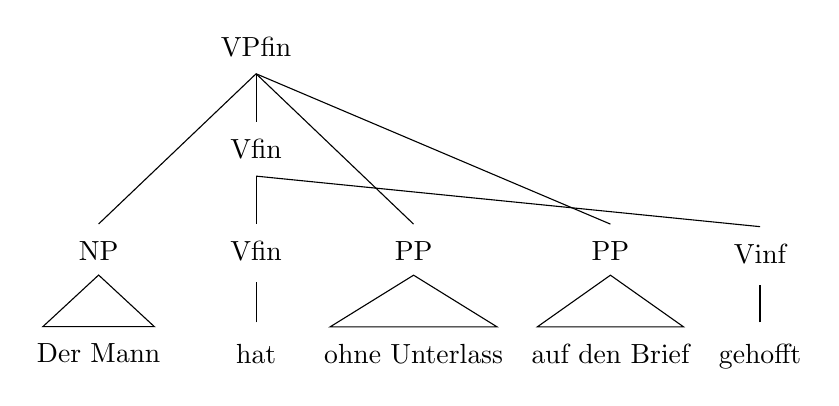
\begin{tikzpicture}[every node/.style={align=center}, line width=0.4pt]

  % --- Parameter ---
  \def\leveldist{1.3}    % vertikaler Abstand zwischen Ebenen
  \def\baseoffset{0.34}  % Dreiecke etwas höher über dem Wort
  \def\triapexgap{0.06}  % größerer Abstand zwischen Label und Dreiecksspitze
  \def\baseinset{0.2}    % Basis leicht kürzer als der Text

  % --- Ebene 1: Wörter (kursiv) ---
  \node (A) at (-3.5,0) [anchor=north] {Der Mann};
  \node (B) at (-1.5,0) [anchor=north] {hat};
  \node (C) at (0.5,0)  [anchor=north] {ohne Unterlass};
  \node (D) at (3.0,0)  [anchor=north] {auf den Brief};
  \node (E) at (4.9,0)  [anchor=north] {gehofft};

  % --- Ebene 2: Kategorien ---
  \node (NP)       at ($(A)+(0,\leveldist)$) {NP};
  \node (Vfinword) at ($(B)+(0,\leveldist)$) {Vfin};
  \node (PP1)      at ($(C)+(0,\leveldist)$) {PP};
  \node (PP2)      at ($(D)+(0,\leveldist)$) {PP};
  \node (Vinfword) at ($(E)+(0,\leveldist)$) {Vinf};

  % --- Dreiecke über den Phrasen ---
  \coordinate (A_baseleft)  at ($(A.west)+(\baseinset,\baseoffset)$);
  \coordinate (A_baseright) at ($(A.east)+(-\baseinset,\baseoffset)$);
  \coordinate (A_top)       at ($(NP.south)-(0,\triapexgap)$);
  \draw (A_baseleft) -- (A_top) -- (A_baseright) -- cycle;

  \coordinate (C_baseleft)  at ($(C.west)+(\baseinset,\baseoffset)$);
  \coordinate (C_baseright) at ($(C.east)+(-\baseinset,\baseoffset)$);
  \coordinate (C_top)       at ($(PP1.south)-(0,\triapexgap)$);
  \draw (C_baseleft) -- (C_top) -- (C_baseright) -- cycle;

  \coordinate (D_baseleft)  at ($(D.west)+(\baseinset,\baseoffset)$);
  \coordinate (D_baseright) at ($(D.east)+(-\baseinset,\baseoffset)$);
  \coordinate (D_top)       at ($(PP2.south)-(0,\triapexgap)$);
  \draw (D_baseleft) -- (D_top) -- (D_baseright) -- cycle;

  % --- Verbindungen Wort → Kategorie (leicht gekürzt + luftiger) ---
  \draw ($(B.north)+(0,0.15)$) -- ($(Vfinword.south)-(0,0.15)$);
  \draw ($(E.north)+(0,0.15)$) -- ($(Vinfword.south)-(0,0.15)$);

  % --- Höhere Ebenen ---
  \node (F) at ($(B)+(0,2*\leveldist)$) {Vfin};
  \node (G) at ($(B)+(0,3*\leveldist)$) {VPfin};

  % --- Verbindungen nach oben (alle mit etwas mehr Luft) ---
  \draw ($(Vfinword.north)+(0,0.1)$) -- ($(F.south)-(0,0.1)$);
  \draw ($(Vinfword.north)+(0,0.1)$) -- ($(F.south)-(0,0.1)$);

  \draw ($(NP.north)+(0,0.1)$)  -- ($(G.south)-(0,0.1)$);
  \draw ($(PP1.north)+(0,0.1)$) -- ($(G.south)-(0,0.1)$);
  \draw ($(PP2.north)+(0,0.1)$) -- ($(G.south)-(0,0.1)$);
  \draw ($(F.north)+(0,0.1)$)   -- ($(G.south)-(0,0.1)$);

\end{tikzpicture}
    \caption{Aufbau einer finiten VP bei Verbzweitstellung}\label{fig:VPinVerbzweit}
\end{figure}

Wie wir in Abschnitt~\ref{section:RegierteVerben} gesehen haben, können auch\is{Verbalphrase (VP)!infinit} Infinitive als Köpfe von VPs fungieren. So handelt es sich bei der infiniten VP \textit{ein paar Bernsteine zu finden} in (\ref{ea:wartetmitINFErg}) bei \textit{ein paar Bernsteine} um die zweite Ergänzung von \textit{zu finden}. Im Unterschied zu finiten VPs wird mit infiniten VPs keine Behauptung (Aussage) gemacht. 

\ea \label{ea:wartetmitINFErg} Anna hofft, [ein paar Bernsteine zu finden].
\z 

Die Struktur der\is{Verbalphrase (VP)!infinit} infiniten VP \textit{ein paar Bernsteine zu finden} wird in Abbildung~\ref{fig:infVPinVerbletzt} dargestellt.

\begin{figure} 
  \centering
  \begin{forest}
      [VPinf, calign=last
        [NP, tier=preterminal [ein paar Bernsteine, narroof]]
        [Vinf, tier=preterminal [zu finden]]
]
  \end{forest}
  \caption{Aufbau einer infiniten VP}\label{fig:infVPinVerbletzt}
\end{figure}

Zu den infiniten Verbalphrasen zählen wir auch Partizipien I (\ref{ea:VPinf_Part1}) und II (\ref{ex:VPinf_Part2}) mit ihren Ergänzungen und Angaben, wenn diese nicht wie bei \textit{die} [\textit{ein paar Bernseine findende}] \textit{Anna} oder \textit{die} [\textit{am Strand gefundenen}] \textit{Bernsteine} adjektivierte Bestandteile einer Nominalphrase oder Bestandteile eines analytischen Verbkomplexes wie bei \textit{sie hat ein paar Bernsteine gefunden} sind. 

\ea \label{ea:VPinf_Part}
\ea \label{ea:VPinf_Part1} [Ein paar Bernsteine findend], spaziert Anna am Strand.
\ex \label{ex:VPinf_Part2} [Ein paar Bernsteine gefunden], geht Anna zufrieden nach Hause.
\z 
\z 

Der Aufbau der infiniten Verbalphrasen \textit{ein paar Bernsteine findend} (\ref{ea:VPinf_Part1}) und \textit{ein paar Bernsteine gefunden} (\ref{ex:VPinf_Part2}) sieht genauso aus wie bei der infiniten VP \textit{ein paar Bernsteine zu finden} in Abbildung~\ref{fig:infVPinVerbletzt}.  

Der Grund für unsere Klassifizierung als infinite Verbalphrase liegt darin, dass Partizipien, also \textit{findend} in (\ref{ea:VPinf_Part1}) und \textit{gefunden} in (\ref{ex:VPinf_Part2}) genauso wie Infinitive infinite Verbformen sind. Um die Unterscheidung zwischen finiten und infiniten Verbformen geht es detailliert in Abschnitt~\ref{subsubsection:finit_infinit}. Hier genügt erst einmal, dass eine Verbform dann infinit ist, wenn sie nicht konjugiert ist, d.\,h. wenn sie keine Person-Numerus-Markierung für eine Subjekt-NP hat. Das ist auch der Grund dafür, dass die infiniten Formen des Verbs \textit{finden} ihre erste Ergänzung, den Findenden, nicht an sich binden können. Formal fehlt ihre erste Ergänzung. Wir müssen sie aus dem Kontext erschließen. In allen drei Fällen verstehen wir \textit{Anna} auch als diejenige, die Bernsteine finden will, findet oder gefunden hat.

In grammatischen Modellen, in denen Sätze in Subjekt und Prädikat bzw. Prädikatsverband zerlegt werden, zählt die erste Ergänzung im Nominativ, die Subjekt-NP, nicht zur VP. Begründet wird dies insbesondere mit dem Mangel an verbspezifischer Rektion (vgl. Abschnitt~\ref{subsubsection:TestFOSP}) sowie mit der Tatsache, dass das finite Verb mit dem Subjekt in Person und Numerus kongruiert. In unserem valenziellen Ansatz zählen wir die Subjekt-NP zur Verbalphrase, differenzieren aber zwischen einer finiten VP und einer infiniten VP.   



\section{Nominalphrase}\label{section:NP}

Die einfachsten\is{Nominalphrase (NP)} Nominalphrasen (NP) bilden Eigennamen wie \textit{Fritzi} in (\ref{ea:NPEigennamen}) und Pronomen wie \textit{der} in (\ref{ex:NPPronomen}).  

\ea \label{ea:NPEigennamenPronomen}
\ea \label{ea:NPEigennamen} \textit{Fritzi} bellt immer.
\ex \label{ex:NPPronomen} \textit{Der} bellt immer.
\z 
\z 

Der Eigenname \textit{Fritzi} und das Pronomen \textit{der} verweisen in den Beispielsätzen (\ref{ea:NPEigennamenPronomen}) auf ein bellendes Lebewesen. Eigennamen sind der prototypische Fall von artikellosen\is{Nominalphrase (NP)!artikellos} NPs im Singular. Genauso bilden Pronomen als Kopf alleine eine NP, was in Abbildung~\ref{fig:NPEigennamenPronomen} dargestellt wird. 

\begin{figure}
\centering
\begin{forest}
    [NP
      [N, tier=preterminal
        [Fritzi]
      ]
    ]
\end{forest}
\hspace{5em}
\begin{forest}
    [NP
      [Pro-N, tier=preterminal
        [der]
      ]
    ]
\end{forest}
\caption{\label{fig:NPEigennamenPronomen}Eigennamen und Pronomen als minimale NP}
\end{figure}

Man könnte die durch das Pronomen gebildete Phrase auch Pro-NP nennen, was die Terminologie jedoch unnötig verkomplizieren würde. Denn strukturell sind NPs und Pronomen gleichwertig, weil Pronomen eben an der Stelle von NPs stehen. Während viele Nomen typischerweise mit anderen Wörtern und Phrasen zur NP ausgebaut werden, können Pronomen diese alleine bilden. Sie können weitgehend analog zu den Nomen nach rechts ausgebaut werden -- was wir in diesem Abschnitt betrachten werden -- aber anders als die Nomen nur sehr begrenzt nach links.\footnote{Der Ausbau nach links ist \zB durch sogenannte Fokuspartikeln wie \textit{sogar} (vgl. Abschnitt~\ref{subsubsection:Fokus}) möglich: [\textit{Sogar der}] \textit{bellt.} Nur einige Indefinit- (vgl. Abschnitt~\ref{subsubsection:Indefinitpronomen}) und die Possessivpronomen (vgl. Abschnitt~\ref{subsubsection:PossPronomen}) können mit einem definiten Artikel eine NP bilden: [\textit{Der meine}] \textit{bellt nie}. [\textit{Der eine}] \textit{bellt immer}.}

Artikellos gebrauchte\is{Nominalphrase (NP)!artikellos} Nomen können alleine eine NP bilden. Dies ist standardmäßig beim indefiniten Plural wie \textit{Hund-e} in \textit{Hunde bellen} der Fall. Neben den bereits erwähnten Eigennamen wie \textit{Fritzi} verwenden wir auch sogenannte Massennomen wie \textit{Gold} und Abstrakta wie \textit{Glück} artikellos als NP wie in \textit{Gold glänzt}.   

Typischerweise sind\is{Nominalphrase (NP)} NPs jedoch komplex. Ein Substantiv wie \textit{Hund} bildet als nominaler Bestandteil den Kopf der NP. Dieser Kopf steht in einem bestimmten Numerus und Kasus und er regiert ein Genus. Allerdings sind das Genus und der Kasus nicht primär am Kopf ersichtlich, sondern an einem Artikelwort wie \textit{der} in (\ref{ea:derHund}), \textit{den} in (\ref{ex:denHund}) oder \textit{dem} in (\ref{ex:demHund}).

\ea 
\ea \label{ea:derHund} Jetzt bellt \textit{der Hund} schon wieder.
\ex \label{ex:denHund} Wir hören \textit{den Hund}.
\ex \label{ex:demHund} Wir geben \textit{dem Hund} einen Knochen.
\z 
\z 

Um die verschiedenen Flexionsformen eines Nomens geht es in Abschnitt~\ref{subsection:Substantivflexion}. Jetzt interessiert uns der Aufbau einer minimalen NP aus Artikel und Nomen. Für \textit{der Hund} stellen wir das Schema in der Abbildung~\ref{fig:ArtNNP} dar.\footnote{Es sei erwähnt, dass man in der generativen Grammatik davon ausgeht, dass bei der Verbindung von Artikel und Nomen der Artikel (Determinierer) der Kopf der ganzen Phrase (Determiniererphrase) ist. Eine kurze Übersicht hierzu bietet \citet[96--98]{Tahiri2022} mit entsprechenden Verweisen auf weiterführende Literatur.}  

\begin{figure}  
\centering
  \begin{forest}
      [NP, calign=last
        [Art, tier=preterminal [der]]
        [N, tier=preterminal [Hund]]
]
  \end{forest}
  \caption{Artikel und Substantiv als minimale NP}\label{fig:ArtNNP}
\end{figure}

Erst\is{Artikelfunktion} der Artikel erlaubt es uns, aus einer nominalen Bedeutungsklasse wie \textit{Hund} auf ein Individuum der Gattung oder auf die Gattung selbst zu verweisen.\footnote{\citet[79--82]{Buehler1934} bezeichnet die Bedeutungsklasse als \textit{Symbolfeld} und die Individualisierung als \textit{Zeigefeld} der Sprache.} Auch der indefinite Artikel \textit{ein} in \textit{ein Hund} führt in vielen Fällen zur Individualisierung, indem auf einen beliebigen Vertreter der Klasse verwiesen wird. Artikel grenzen das Substantiv in Bezug auf seinen Geltungsbereich ein.\footnote{\citet[18]{Agel1996} schreibt daher auch vom \textit{finiten Substantiv}. Allerdings macht \citet[32]{Agel1996} deutlich, dass eine echte syntaktische Nominalklammer nicht aus Artikel und Nomen, sondern aus dem Flexionsteil, welcher typischerweise der Artikel trägt, und dem Nomen besteht, also \zB \textit{de}[\textit{r}--\textit{Hund}]. Dies wird deutlich, wenn der Flexionsteil am Adjektiv realisiert wird wie in \textit{klein}[\textit{er}--\textit{Hund}]. Um die Flexion innerhalb der NP geht es in den Abschnitten~\ref{subsection:Artikel_SGr_Flexion} und \ref{subsection:Adjektiv_SGr_Flexion}.}


So wie die Teile des Verbkomplexes in Verberst- und Verbzweitsätzen eine Klammer und somit Felder bilden (vgl. Einführung ins Kapitel \ref{chapter:Feldermodell}), so bilden auch das Artikelwort und das Substantiv eine\is{Nominalklammer} Klammer. Zwischen dem Artikel und dem Nomen können flektierte Adjektive stehen. Die Klammeranalogie wird in der Abbildung~\ref{fig:Nominalklammer} dargestellt. Der linken Satzklammer (LSK) entspricht die linke Nominalklammer (LNK), der rechten Satzklammer (RSK) die rechte Nominalklammer (RNK).   

\begin{figure}
  
  \begin{tabular}{cp{0.1em}cp{0.1em}cp{0.1em}c}
    LSK/LNK && MF && RSK/RNK && \\
    \cmidrule{1-1}\cmidrule{3-3}\cmidrule{5-5}
    hat && der Hund && gebellt \\
    der && kleine && Hund \\
  \end{tabular}
  \caption{Nominalklammer als Analogon zur Verbalklammer}
  \label{fig:Nominalklammer}
\end{figure}


\citet[355--356]{Weinrich2003} beschreibt die\is{Nominalklammer} Nominalklammer als \gqq{Analogon} zur Verbalklammer. So wie das Finitum die Kategorien Person, Numerus, Tempus, Modus und Genus verbi markiert, das Verb damit eingrenzt (Finitum) und das Subjekt via Kongruenz in die Verbgruppe einbindet, so markiert der Artikel die Genus-, Kasus- sowie sekundär Numeruskategorien und stellt typischerweise Referenz auf einen definiten (konkreten) oder indefiniten (beliebigen) Vertreter der vom Substantiv bezeichneten Klasse her. 

\begin{Exkurs}{Funktion der Klammer}
 
\citet[95]{Ronneberger-Sibold2010} beschreibt die grundlegende Funktion der Klammer als \gqq{Erleichterung der syntaktischen Dekodierung} wie folgt: 

\begin{quote}
    
Dadurch, dass die jeweils zueinander passenden Klammerränder die Grenzen von (verschieden definierten) Konstituenten klar markieren, wissen die Hörer/Leser bzw. die Hörerinnen/Leserinnen während des Dekodierungsprozesses jederzeit, ob sie sich am Anfang, im Inneren oder am Ende einer Konstituente befinden. \citep[95]{Ronneberger-Sibold2010}  

\end{quote}
\citet[356]{Weinrich2003} weist auf einen anderen Effekt hin. Der Hörer muss die Informationen aus dem MF solange in seinem Kontextgedächtnis speichern, bis er das Verb in der RSK bzw. das Nomen in der RNK rezipiert. Dies erzeuge einen Spannungsbogen, der durch die rechte Klammer aufgelöst wird. 

Für \citet[223--236]{Bittner2010} haben beide Klammertypen keine eigenständigen Funktionen. Die Klammerbildung resultiere aus der sprachspezifischen Umsetzung von informationsstrukturellen Maximen: die Voranstellung des Finitums kennzeichnet Fragen und Aussagen (vgl. \textit{Illokution} Einführung Kapitel~\ref{chapter:Feldermodell}), die Endstellung des infiniten Vollverbs folgt der Informationsgewichtung, nach der neue Informationen (indefinit bzw. infinit) weit rechts stehen (vgl. Abschnitt~\ref{subsection:Mittelfeld}). Die Satzklammer wird diesen Anforderungen gerecht. Analog zum Finitum eröffnet der Artikel die Nominalklammer und determiniert das rechts stehende Nomen. Damit werden sowohl die Verbal- als auch die Nominalklammer durch ein grammatisches Element eröffnet, das die Bedeutung des am Ende stehenden Nomens aktualisiert.  

Auf die didaktische Nutzung der Nominalklammer bei der Vermittlung der satzinternen Großschreibung (Substantivgroßschreibung) gehen wir gesondert im Exkurs~\ref{ex:Treppenwoerter} in Kapitel~\ref{kap:Graphematik} ein, wo es um die Prinzipien der Schreibung des Deutschen geht.

\end{Exkurs}

Einen Sonderfall in der NP stellen vorangestellte genitivische Eigennamen wie in \textit{Fritzis Fressnapf} und als solche gebrauchte Verwandtschaftsbeziehungen wie in \textit{Omas Liebling} dar. Die Erweiterung durch die pränominale NP im Genitiv hat auch Artikelfunktion. Das ist auch bei den genitivischen Relativpronomen \textit{deren} und \textit{dessen} in \textit{Anna und deren Bruder} oder \textit{Paul und dessen Bruder} der Fall.\footnote{Die Voranstellung des Genitivs ist die historisch ältere Form und geschah vor Ausbildung des Artikels. Bei Ausbildung des Artikelgebrauchs wurde der vorangestellte Genitiv als definites Artikelwort reanalysiert; cf. \citet[231]{Demske2001}. Artikelwort und pränominaler Genitiv können deshalb nicht zusammen vorkommen: *\textit{der Fritzis Fressnapf}. Die vorangestellte genitivische NP besetzt zwar die Stelle des definiten Artikels, ist aber selbst keiner. Das zeigt sich bei der Flexion des Adjektivs (vgl. Abschnitt~\ref{subsection:Adjektiv_SGr_Flexion}): \textit{der neu-e Fressnapf} versus \textit{Fritzis neu-er Fressnapf}. Bei Interesse verweisen wir auf \citet{Eichinger2006}.}

In der\is{Nominalklammer!Mittelfeld} Nominalklammer können flektierte Adjektive wie \textit{kleine} in \textit{der kleine Hund} stehen. Die Adjektive hängen vom Nomen ab. Ihre Funktion ist es, Werte von Eigenschaften festzulegen, über die das Nomen bzw. die von der NP bezeichnete Entität verfügt. So legt \textit{kleine} den Wert der Eigenschaft Größe fest, über die der bezeichnete Hund verfügt. Der Unterschied zur verbalen Prädikation besteht darin, dass mit \textit{der kleine Hund} nicht explizit behauptet wird, dass der Hund klein ist.\footnote{\citet[317]{Eichinger1991} beschreibt die Merkmalsübertragung durch Adjektive als \gqq{implizite Prädikation}. \citet[140]{Paul1880} bezeichnet Merkmalsbestimmungen dieser Art als \gqq{degradiertes Prädikat}.} Sie kann explizit gemacht werden, wenn das Adjektiv mit \textit{sein} prädikativ gebraucht wird wie in \textit{der Hund ist klein}. Darum geht es im Abschnitt~\ref{subsection:SP und OP}. 

Auch Adjektive bilden Phrasen. Wir könnten statt \textit{kleine} in \textit{der kleine Hund} auch \textit{der sehr kleine Hund} sagen. Um den Bau von Adjektivphrasen (APs) geht es in Abschnitt~\ref{section:AP}. Hier interessiert erst einmal nur der Aufbau der NP mit einer AP als Konstituente. Dies wird in Abbildung~\ref{fig:NPmitAP} dargestellt.


\begin{figure}
  \centering
  \begin{forest}
    [NP, calign=child, calign child=3
      [Art, tier=preterminal
        [der]
      ]
      [AP, tier=preterminal
        [sehr kleine, narroof]
      ]
      [N, tier=preterminal
        [Hund]
      ]
      ]
  \end{forest}
  \caption{Ausbau der NP durch eine AP}
  \label{fig:NPmitAP}
\end{figure}

Theoretisch\is{Nominalklammer!Mittelfeld} können beliebig viele APs in der Nominalklammer stehen. Denn man könnte immer wieder eine AP hinzufügen: \textit{der sehr kleine Hund} oder \textit{der freundliche sehr kleine Hund} oder \textit{der erste freundliche sehr kleine Hund} usw.  

\newpage
\begin{Exkurs}{Reihenfolge der Adjektive in der Nominalklammer}
    
\largerpage
Um\is{Nominalklammer!Mittelfeld} die Abfolge der Adjektivphrasen (APs) zu erklären, schlägt \citet[317]{Eichinger1991} ein plurizentrisches Modell vor. In diesem bildet der Artikel einen Pol und das Nomen den anderen. Die APs stehen entweder beim Artikel oder beim Nomen. 

In Artikelnähe stehen Zahladjektive. Denn sie bauen explizit die Quantifikation aus, die im Artikel implizit angelegt ist. Der definite Artikel im Singular wie bei \textit{der Hund} impliziert Einzahl, welche durch ein Zahladjektiv explizit gemacht werden kann wie in \textit{der eine Hund}. Dies ist freilich im Plural viel relevanter, da die Mehrzahl bei \textit{die Hunde} sowohl für \textit{die zwei Hunde} als auch für \textit{die vierhundert Hunde} gelten kann.  

Adjektive\is{Nominalklammer!Mittelfeld}, die eine zeitliche und örtliche Eingrenzung des Bezugsnomens leisten, stehen ebenfalls in Artikelnähe, nach den Zahladjektiven (falls vorhanden). Denn sie vervollständigen die im Artikel angelegte Individualisierung eines konkreten Referenten. Daher heißt es typischerweise \textit{die zwei damaligen Schüler} oder \textit{die zwei hiesigen Schulen}. 

Eine\is{Nominalklammer!Mittelfeld} Art Zwischenstellung zwischen dem Artikelpol und dem Nominalpol nehmen nach \citet[321]{Eichinger1991} die Adjektive ein, die Eigenschaften im Sinne einer impliziten \textit{sein}-Prädikation ausdrücken. Dabei handelt es sich um bewertende Adjektive wie \textit{unkompliziert}, \textit{überraschend} oder \textit{altmodisch} und um Adjektive, die relative Qualitäten wie \textit{groß} oder \textit{alt} ausdrücken. Hierbei handelt es sich um mehr oder weniger typische Eigenschaften von Nominalklassen wie Alter bei Lebewesen oder Größe von Objekten. Wenn beide Adjektivtypen vorkommen, steht das bewertende Adjektiv zuerst, da ja gerade der Komplex aus Eigenschaft und Nomen bewertet wird. Als Beispiele führt \citet[321]{Eichinger1991} Belege wie \textit{diese altmodischen kleinen Gesänge} und \textit{ein entzückendes kleines Palais} an. Denn \textit{die kleinen Gesänge sind altmodisch} und \textit{das kleine Palais ist entzückend}.

Dem nominalen Pol am nächsten stehen\is{Nominalklammer!Mittelfeld} Adjektive, die in der Regel nicht steigerbare Werte absoluter Merkmale festlegen. Bei Konkreta handelt es sich um Merkmale wie Form, Farbe und Material. Deshalb scheint die Abfolge in \textit{ein großer runder Tisch} und \textit{eine kleine blaue Blüte} natürlicher als in \textit{ein runder großer Tisch} und \textit{eine blaue kleine Blüte}. Ebenfalls am nominalen Pol stehen Adjektive, die das Nomen zu Sachbereichen zuordnen wie \textit{die chemische Industrie} oder \textit{der sportliche Ehrgeiz}. Hier wird ein Bereich der Chemie zugeordnet und der Ehrgeiz auf den Sport bezogen. \citet[324]{Eichinger1991} bezeichnet sie als \textit{Nominalklassifikationen}, die eher zu Kategoriebildungen führen.

\end{Exkurs}


Bei\is{Nominalklammer!Mittelfeld} mehreren aufeinanderfolgenden APs wie in (\ref{ea:mehrereAP}) kann es sich trotz formaler Ähnlichkeit um sehr unterschiedliche Strukturen handeln. Man vergleiche (\ref{ea:AP,AP}) mit (\ref{ex:APAP}).  

\ea \label{ea:mehrereAP}
\ea \label{ea:AP,AP} kluge, unterhaltsame Bücher
\ex \label{ex:APAP} spannende französische Bücher
\z 
\z 

Die Bedeutungen von zwei oder mehreren APs können sich wie in (\ref{ea:AP,AP}) gleichrangig (koordiniert) auf ein Nomen beziehen. In diesem Fall setzt man ein Komma. Die koordinierte Lesart kann durch \textit{und} zwischen beiden APs getestet werden (\ref{ea:APgleichrangigmitKOOR}).

\ea \label{ea:APgleichrangigmitKOOR} kluge und unterhaltsame Bücher
\z 

Strukturell\is{Nominalklammer!Mittelfeld} verbinden sich die beiden APs zu einem koordinierten AP-Komplex und dieser wird dann auf das Nomen übertragen. Dies stellen wir in der Abbildung~\ref{fig:koordinierteAPinNP} dar.


\begin{figure}
  \centering
  \begin{forest}
    [NP, calign=last
      [AP, calign=child, calign child=2
        [AP, tier=preterminal
          [kluge\\ kluge, narroof]
        ]
        [Koordination, tier=preterminal
          [{und\\,}]
        ]
        [AP, tier=preterminal
          [unterhaltsame\\unterhaltsame, narroof]
        ]
      ]
      [N, tier=preterminal
        [Bücher\\Bücher]
      ]
    ]
  \end{forest}
  \caption{Koordinierte APs in der NP}
  \label{fig:koordinierteAPinNP}
\end{figure}


Hiervon zu unterscheiden sind Fälle, in denen sich die\is{Nominalklammer!Mittelfeld} APs schrittweise nacheinander auf das Nomen beziehen wie in (\ref{ex:APAP}). Die beiden APs verstehen wir, zumindest in der üblichen Lesart, nicht koordiniert. Zuerst verbindet sich \textit{französische} mit \textit{Bücher} und die AP \textit{spannende} bezieht sich auf den Komplex \textit{französische Bücher.} In dieser üblichen Lesart kann kein \textit{und} zwischen den APs stehen (\ref{ea:APschrittweise*und}). 

\ea \label{ea:APschrittweise*und} ? spannende und französische Bücher
\z 

Die Struktur stellen wir in der Abbildung~\ref{fig:schrittweiseAPAPNP} dar. 

\begin{figure}
  \centering
  \begin{forest}
    %l sep+=2em
    [NP, calign=last
      [AP, tier=preterminal
        [spannende, narroof]
      ]
      [N, calign=last
        [AP, tier=preterminal [französische, narroof]]
        [N, tier=preterminal [Bücher, tier=terminal]]
]
    ]
  \end{forest}
  \caption{Schrittweise Verbindung der APs mit der NP}\label{fig:schrittweiseAPAPNP}
\end{figure}

\begin{Exkurs}{Nachgestellte Adjektive}
    
Zur besonderen Hervorhebung kann das Bezugsnomen alleine vorangestellt werden. Das flektierte Adjektiv steht dann außerhalb der Nominalklammer, also in Distanz zum Kopf wie in (\ref{ea:flektierteAPpostnominal}). Typisch ist ihr Anschluss mit \textit{nur} oder \textit{und zwar}.   

\ea \label{ea:flektierteAPpostnominal} Hier gibt es Bücher ab zwei Euro, und zwar neue.\footnote{Die Presse, 09.06.2008.}
\z 

Auch diese APs sind Konstituenten der\is{Nominalphrase (NP)} NP. Der vorangehende nominale Kopf wird als Bezugsnomen mitverstanden als \textit{und zwar neue Bücher}. 

Ein\is{Nominalphrase (NP)} anderer Sonderfall\is{Nominalklammer!Nachfeld} nachgestellter Adjektive findet sich in dem Kinderlied \textit{Hänschen klein} oder in Goethes \textit{Heidenröslein}, wo es heißt \textit{Röslein rot}. Analoge Bildungen sind \textit{Forelle blau} oder \textit{Apfelkuchen süß und saftig}. Die Adjektive sind nicht flektiert und das Nomen wird artikellos gebraucht. Der Konstruktionstyp gilt als archaisch.\footnote{\citet[29]{Behaghel1927} sagt in einem 1899 gehaltenen Vortrag: \gqq{Wenn das Volkslied noch immer singt von \textit{Röslein rot}, so bewahrt es damit eine Wortstellung, die seit etwa einem Jahrtausend in der lebendigen Sprache abgestorben ist.}} \citet[63]{Duerscheid2002} analysiert diese Stellung funktional: \gqq{Das Element mit dem höheren Grad an kommunikativer Dynamik [das Nomen, MF] steht in der linearen Abfolge an erster Stelle, dann folgt dasjenige mit dem niedrigeren Mitteilungswert, der erläuternde Zusatz}. Die Nicht-Flektiertheit des Adjektivs ist insofern regelkonform, als dass Adjektive als Konstituenten einer NP nur innerhalb der Nominalklammer flektiert werden. Als Ausnahmen hiervon führt die \citet[455, §750]{Duden2022} feste Wendungen aus älteren Sprachstufen auf wie \textit{Gut Ding will Weile haben} und geprägte Verwendungen wie \textit{warm Wasser}. Zu diesem Muster gehören auch \textit{klein Erna} und \textit{lütt Matten}. 

Einen\is{Nominalphrase (NP)} speziellen Typ der unflektierten\is{Nominalklammer!Nachfeld} Nachstellung von Adjektiven zeigen Bildungen wie \textit{Romantik pur}, \textit{Sonne satt}, \textit{Party total} oder \textit{Gesetz light}. Diese nachgestellten Adjektive sind keine Eigenschaftszuweisungen im engeren Sinne, sondern bringen häufig, so \citet[67]{Duerscheid2002}, \gqq{eine wertende Sprechereinstellung zum Ausdruck}. 

Wir kommen unter dem Stichwort \textit{Apposition} im Exkurs~\ref{subsection:Apposition} auf jene Konstruktionen zurück. In Bezug auf die nachgestellten Adjektive gilt, dass die von ihnen gebildeten APs Bestandteile, also Konstituenten von NPs sind, was in \ref{fig:nachgestellteAP} dargestellt wird.

\begin{figure}
  \centering
  \begin{forest}
    [NP, calign=child, calign child=1
      [N, tier=preterminal
        [Hänschen\\Innenwandfarbe\\Romantik]
      ]
      [AP, tier=preterminal
        [klein\\weiß und waschbeständig\\pur]
      ]
      ]
  \end{forest}
  \caption{Ausbau der NP durch eine nachgestellte AP}
  \label{fig:nachgestellteAP}
\end{figure}

\end{Exkurs}

Typischerweise stehen\is{Nominalklammer!Nachfeld} im nominalen Nachfeld, d.\,h. nach dem Kopfnomen, NPs im Genitiv, PPs und Relativsätze. Da innerhalb der Nominalklammer die Flexion der einzelnen Elemente zusammenspielt (\textit{der kleine Mann/ein kleiner Mann}), wird die Ausklammerung von NPs im Genitiv, von PPs und Relativsätzen verständlich. Sie würden die Klammerflexion nämlich blockieren. Das Gleiche wäre der Fall bei Adverbien, die zwar typischerweise Bestandteile von VPs sind, aber auch postnominal wie \textit{der Baum dort} oder \textit{der Film gestern} gebraucht werden. 

Postnominale\is{Nominalklammer!Nachfeld} NPs im Genitiv und PPs ähneln sich funktional, was anhand von \textit{der kleine Hund meiner Schwester} und \textit{der kleine Hund von meiner Schwester} deutlich wird. Relativsätze stehen ganz am Ende der NP.  

Es mag sein, dass die Analogie zum Nachfeld in Sätzen didaktisch hilfreich ist, weshalb wir postnominale Erweiterungen in Abbildung~\ref{fig:postnominalerNPAusbau} darstellen.


\begin{figure}
  
  \begin{tabular}{cp{0.1em}cp{0.1em}cp{0.1em}c}
    LNK && MF && RNK && NF \\
    \cmidrule{1-1}\cmidrule{3-3}\cmidrule{5-5}\cmidrule{7-7}
    der && kleine && Hund && meiner Schwester \\
    der && kleine && Hund && aus Berlin \\
    der && kleine && Hund, && den wir streicheln\\ 
     der && kleine && Hund && meiner Schwester, den wir streicheln\\ 
  \end{tabular}
  \caption{Postnominale Erweiterungen der NP}
  \label{fig:postnominalerNPAusbau}
\end{figure}

In der Abbildung~\ref{fig:komplexeNP} stellen wir die Konstituentenstruktur der\is{Nominalphrase (NP)} NP \textit{der kleine Hund meiner Schwester, den wir streicheln} dar. 


\begin{figure}
  \centering
  \begin{forest}
    [NP, calign=child, calign child=3
      [Art, tier=preterminal
        [der]
      ]
      [AP, tier=preterminal
        [kleine]
      ]
      [N, tier=preterminal
        [Hund]
      ]
      [NP, tier=preterminal
        [meiner Schwester{,}, narroof]
      ]
      [Relativsatz, tier=preterminal
        [den wir streicheln, narroof]
      ]
    ]
  \end{forest}
  \caption{Ausbau der NP durch eine AP, eine NP und einen Relativsatz}
  \label{fig:komplexeNP}
\end{figure}

Grundlegende Unterschiede zwischen dem Ausbau des Verbkopfes zur VP und des Nominalkopfes zur NP sowie deverbale Nominalisierungen behandeln wir im Abschnitt~\ref{section:SatzgliederundAttribute}, in dem es um Satzglieder im Unterschied zu Attributen geht. Bevor wir den Bau von Adjektivphrasen (APs) im Abschnitt~\ref{section:AP} untersuchen, geht es im folgenden Exkurs~\ref{subsection:Apposition} um Appositionen, d.\,h. um komplexe NPs wie \textit{Chaplin, der berühmte Schauspieler} oder \textit{der berühmte Schauspieler Chaplin}.   


\begin{Exkurs}{Appositionen}\label{subsection:Apposition}

Komplexe NPs\is{Apposition} wie \textit{Chaplin, der berühmte Schauspieler} bestehen aus einem Eigennamen, hier \textit{Chaplin}, und einer folgenden NP, hier \textit{der berühmte Schauspieler}. Beide können referenzidentisch sein, d.\,h. sowohl mit \textit{Chaplin} als auch mit \textit{der berühmte Schauspieler} kann dieselbe außersprachliche Person oder Sache bezeichnet werden. Die Funktion dieser Konstruktion ist es, dem vom Eigennamen bezeichneten Individuum charakteristische Merkmale zuzuweisen, um dem Kommunikationspartner, wie \citet[33]{Zifonun2015} schreibt, \gqq{den Anschluss an sein Wissen} zu ermöglichen. 

In (\ref{ea:Apposition}) beziehen sich der Eigenname \textit{Chaplin} und die Erläuterung \textit{der berühmte Schauspieler} auf ein und dieselbe außersprachliche Person. Jene Erläuterungen in Form einer NP nennt man\is{Apposition} \textit{Apposition}. Sie bilden zusammen mit ihrem Bezugswort \textit{eine} NP.\footnote{Welche Strukturen unter \textit{Apposition} fallen und welche nicht, ist stark umstritten und interessiert hier nicht. Eine knappe Übersicht gibt \citet[32--34]{Zifonun2015}.} 

\ea \label{ea:Apposition}
\ea \label{ea:weiteApp} Chaplin, der berühmte Schauspieler, brachte viele zum Lachen.
\ex \label{ex:engeApp} Der berühmte Schauspieler Chaplin brachte viele zum Lachen.
\z 
\z 

Nach \citet[511]{HelbigBuscha} wird meist zwischen lockeren Appositionen wie (\ref{ea:weiteApp}) und\is{Apposition!locker} engen, d.\,h. integrierten Appositionen (\ref{ex:engeApp}) unterschieden. 

In (\ref{ea:weiteApp}) handelt es sich bei \textit{der berühmte Schauspieler} um eine \textit{lockere Apposition}. Sie hebt sich durch eine Sprechpause vom Bezugswort \textit{Chaplin} ab, was schriftlich durch ein Komma gekennzeichnet wird. Die appositive NP gibt zusätzliche Informationen über den Referenten des Bezugsnomens. Sie stellt eine zusätzliche Prädikation (Merkmalszuweisung) dar. 

Typischerweise kongruiert die\is{Apposition!locker} appositive NP hinsichtlich des Kasus des Kopfes.\footnote{\textit{Typischerweise}, da insbesondere beim artikellosen Gebrauch keine Kasusmarkierung möglich ist bzw. der Nominativ als unmarkierter Kasus steht wie in \textit{Chaplin, Schauspieler und Regisseur, brachte viele zum Lachen}. Ebenso gibt es tolerierte Abweichungen wie bei der Angabe des Datums \textit{am Freitag, dem 13.} oder \textit{am Freitag, den 13.} Eventuell wird hier der temporale Akkusativ aus \textit{Berlin, den 13.} kopiert. Wenn das Bezugsnomen im Genitiv steht, wird die appositive NP umgangssprachlich auch im Dativ ausgedrückt wie in dem folgenden Internetbeleg: \textit{die Vita Dieter Müllers, dem Botschafter des außergewöhnlichen Geschmacks}. Laut \citet[444--445, §730]{Duden2022} gilt dieser inkongruente Dativ in der Standardsprache als nicht korrekt. Korrekt müsste es heißen: \textit{die Vita Dieter Müllers, des Botschafters des außergewöhnlichen Geschmacks}.} 
In (\ref{ea:weiteApp}) stehen beide im Nominativ, in (\ref{ea:KongruenzAkk}) im Akkusativ, in (\ref{ex:KongruenzDat}) im Dativ und in (\ref{ex:KongruenzGen}) im Genitiv, wo die Kongruenz durch das Flexiv \textit{-s} sichtbar ist.

\ea \label{ea:KongruenzweiteApposition}
\ea \label{ea:KongruenzAkk} Ohne Chaplin, \textit{den} berühmten Schauspieler, hätten wir weniger gelacht.
\ex \label{ex:KongruenzDat} Mit Chaplin, \textit{dem} berühmten Schauspieler, haben viele gelacht.  
\ex \label{ex:KongruenzGen} Die Autobiographie Chaplin\textit{s}, \textit{des} berühmten Schauspieler\textit{s}, ist weniger bekannt.
\z 
\z 

Die Struktur der\is{Apposition!locker} NPs in (\ref{ea:KongruenzweiteApposition}) stellen wir in der Abbildung~\ref{fig:NPmitAppkongruent} dar. 


\begin{figure}
  \centering
  \begin{forest}
    [NP, calign=child, calign child=1
      [NP, calign=child, calign child=1
        [N, tier=preterminal
        [Chaplin{,}]
      ]
      ]
      [NP, tier=preterminal
        [der berühmte Schauspieler, narroof]
      ]
      ]
  \end{forest}
  \caption{Lockere Apposition}
  \label{fig:NPmitAppkongruent}
\end{figure}

Der Kopf der lockeren Apposition ist der Eigenname \textit{Chaplin}. Eigennamen können, wie wir in Abschnitt~\ref{section:NP} gesehen haben, alleine eine NP bilden. Dies ist auch innerhalb dieser lockeren Apposition der Fall. Der Eigenname ist erweiterbar: \textit{der kleine Chaplin, der berühmte Schauspieler}. Auch die Apposition \textit{der berühmte Schauspieler} ist eine NP. Jede der beiden NPs kann anstelle der anderen NP gebraucht werden: \textit{Chaplin brachte viele zum Lachen} oder eben \textit{der berühmte Schauspieler brachte viele zum Lachen}. Allerdings sind beide NPs nicht gleichrangig wie in einer koordinierten Struktur. Denn bei Koordination durch \textit{und} wird die Referenzidentität aufgehoben: \textit{Chaplin und der berühmte Schauspieler}. Die appositive NP ist der ersten NP locker beigeordnet. 

Wir folgen \citet[2037]{ZifHoffStr1997} und zählen auch nachgestellte Adjektive bzw. Adjektivphrasen wie in (\ref{ea:unflAPalsAPP}) zu den\is{Apposition} Appositionen. Auch bei diesen handelt es sich um eine Art Nachtrag zum nominalen Kopf der gesamten NP. Bildlich beschreibt \citet[777]{Agel2017} diese als \gqq{Verlängerung} der NP und \gqq{Wortgruppenrandglied}. \citet[531]{Weinrich2003} hält jenen Nachtrag oder Anbau (statt Integration) dadurch für motiviert, dass die Nominalklammer entlastet wird und dass jene Nachträge \gqq{in ihrer Bedeutung auffällig gemacht} werden. Typischerweise handelt es sich um zwei koordinierte Adjektive wie in (\ref{ea:unflAPalsAPP}) oder ein erweitertes Partizip wie in (\ref{ex:unflPart}).

\ea \label{ea:nachgestellte AP}
\ea \label{ea:unflAPalsAPP} Wir bieten eine komfortable Wohnung, hell und ruhig, zur Zwischenmiete.
\ex \label{ex:unflPart} Bieten tolle 3-Zi-Wohnung, frisch renoviert, mit Balkon und EBK.
\z
\z 

Lockere Appositionen\is{Apposition!locker} sind nur schwach in die NP des Bezugsnomens integriert. Dies wird deutlich, wenn sie nicht auf das Bezugsnomen folgen, sondern von ihm getrennt im Nachfeld eines Satzes erscheinen (\ref{ea:APPimNFbeiNomen}). Typisch ist die Stellung im Nachfeld, wenn das Bezugswort ein Pronomen ist (\ref{ex:APPimNFbeiPrn}). Genauso können auch APs nachgestellt werden (\ref{ex:APPimNFmitAP}).

\ea \label{ea:APPimNF}
\ea \label{ea:APPimNFbeiNomen} Chaplin brachte viele zum Lachen, dieser berühmte Schauspieler.
\ex \label{ex:APPimNFbeiPrn} Er brachte viele zum Lachen, der berühmte Schauspieler.
\ex \label{ex:APPimNFmitAP} Wir bieten eine komfortable Wohnung zur Zwischenmiete, hell und ruhig. 
\z 
\z 

Sogenannte \textit{enge} Appositionen\is{Apposition!eng} wie \textit{der Schauspieler Chaplin} verhalten sich anders. Hier ist \textit{Schauspieler} der Kopf, in den der appositive Eigenname integriert ist. Dieser ist kein Nachtrag oder Zusatz, sondern referenznotwendig. Ohne ihn wüssten wir nicht, welche Person oder Entität bezeichnet wird. Deshalb bezeichnet die \citet[448, §737]{Duden2022} die Funktion dieser engen Apposition als \textit{explikativ}. 

Die Kasusmarkierung der gesamten NP zeigt sich am Artikel und im Genitiv auch am Kopfnomen: \textit{des Schauspielers}. Der appositive Eigenname bildet hier selbst keine Phrase. Es handelt sich um ein nicht erweiterbares Nomen: *\textit{der berühmte Schauspieler kleiner Chaplin}. Der Eigenname \textit{Chaplin} bleibt unverändert im Nominativ als unmarkierter Kasus. Beim Genitiv wird dies beim Vergleich von \textit{Chaplins} in (\ref{ex:KongruenzGen}), hier als (\ref{ea:KongruenzGen1}) wiederholt, mit \textit{Chaplin} in (\ref{ex:keineKongruenzGen}) deutlich.

\ea 
\ea \label{ea:KongruenzGen1} Die Autobiographie \textit{Chaplins}, des berühmten Schauspielers, ist weniger bekannt. 
\ex \label{ex:keineKongruenzGen} Die Autobiographie des berühmten Schauspielers \textit{Chaplin} ist weniger bekannt.
\z 
\z 

\citet[281]{Eisenberg2020_Satz} bezeichnet die Nominativrektion als konstruktionell. Denn der Nominativ wird weder von der Kategorie Nomen noch von einzelnen Nomen regiert, sondern von der Appositionskonstruktion.\footnote{Kategorial regieren Nomen nur den Genitiv wie in \textit{der Hund des Nachbarn}.} Das Gleiche ist der Fall bei vorangestellten Verwandtschafts-, Titel- oder Berufsbezeichnungen, wenn diese einen Artikel haben wie: \textit{mein Onkel Paul}, \textit{der bekannte Professor Eisenberg} oder \textit{der beliebte Bäcker Hacker}. Nur der Artikel und im Genitiv auch das Kopfnomen tragen die Kasusmarkierung der gesamten NP (\ref{ea:meinesOnkelsPaul}). Der appositive Eigenname muss im Nominativ stehen, weshalb (\ref{ex:meinesOnkels*Pauls}) ungrammatisch ist.

\ea \label{ea:meinOnkelPaul}
\ea [] {das Haus meines Onkels \textit{Paul}}\label{ea:meinesOnkelsPaul} 
\ex [*] {das Haus meines Onkels \textit{Pauls}}\label{ex:meinesOnkels*Pauls}
\z 
\z 

Den\is{Apposition!eng} Aufbau der NPs \textit{der Schauspieler Chaplin} und \textit{mein Onkel Paul} stellen wir in Abbildung~\ref{fig:NPmitAppNominativ} dar.


\begin{figure}
\centering
  \begin{forest}
    [NP, calign=child, calign child=2
      [Art, tier=preterminal
        [der\\mein]
      ]
      [N, tier=preterminal
        [Schauspieler\\ Onkel]
      ]
      [N, tier=preterminal
        [Chaplin\\Paul]
      ]
      ]
  \end{forest}
  \caption{Enge Apposition}
  \label{fig:NPmitAppNominativ}
\end{figure}


Diese\is{Apposition!eng} Verhältnisse drehen sich um, wenn das erste Nomen zum Ausdruck einer Verwandtschafts-, Titel- oder Berufsbezeichnung artikellos gebraucht wird, wie in \textit{Onkel Paul}, \textit{Professor Eisenberg} oder \textit{Bäcker Hacker}. In diesen Fällen ist der Eigenname der Kopf der NP, denn er trägt die Kasusmarkierung der NP. Der Nominativ des appositiven Nomens ist konstruktionell regiert. Dies wird wieder beim Genitiv deutlich (\ref{ea:OnkelPaul}). Der Eigenname als Kopf trägt die Genitivmarkierung (\ref{ea:OnkelPauls}). Der appositive Eigenname muss im Nominativ stehen, weshalb (\ref{ex:Onkels*Pauls}) ungrammatisch ist.

\ea \label{ea:OnkelPaul}
\ea [] {das Haus \textit{Onkel} \textit{Pauls}}\label{ea:OnkelPauls}
\ex [*] {das Haus \textit{Onkels} \textit{Pauls}}\label{ex:Onkels*Pauls}
\z 
\z  

Den Aufbau der NPs \textit{Onkel Paul} und \textit{Professor Eisenberg} zeigen wir in Abbildung~\ref{fig:APPmitEigennamenKopf}. Da sich die Verbindung von Vor- und Nachnamen wie \textit{Peter Eisenberg} genauso gestaltet, führen wir sie mit auf.


\begin{figure}
  \centering
  \begin{forest}
    [NP, calign=child, calign child=2
      [N, tier=preterminal
        [Onkel\\ Professor\\ Peter]
      ]
      [ N, tier=preterminal
        [Paul\\ Eisenberg\\ Eisenberg]
      ]
      ]
  \end{forest}
  \caption{Enge Apposition}
  \label{fig:APPmitEigennamenKopf}
\end{figure}

\newpage
In \textit{Onkel Paul} ist \textit{Paul} der Kopf und \textit{Onkel} die\is{Apposition!eng} Apposition. Im Gegensatz dazu ist in \textit{mein Onkel Paul} der Eigenname \textit{Paul} die Apposition und \textit{Onkel} der Kopf. Verständlich wird jenes \gqq{Umkippen der Abhängigkeitsverhältnisse}, wie \citet[282]{Eisenberg2020_Satz} schreibt, vor dem Hintergrund der analytischen Nominalflexion. Wie wir gesehen haben, sind minimale NPs typischerweise zweigliedrig, sie bestehen aus einem Artikel und dem Nomen wie \textit{mein Onkel} und \textit{der Professor}. Wenn der Artikel jedoch fehlt wie in \textit{Onkel Paul}, dann kann das Nomen \textit{Onkel} im Genitiv nicht mehr das Nominalflexiv \textit{-s} tragen, da dessen Realisierung an die analytische Flexion mit Artikel gebunden ist. Daher heißt es \textit{das Haus mein-es Onkel-s Paul} aber nicht *\textit{das Haus Onkel-s Paul}. In diesem Fall trägt der Eigenname das Genitivflexiv und ist Kopf der NP: \textit{das Haus Onkel Paul-s}. Denn Eigennamen verfügen unabhängig von ihrem Genus über synthetische Genitivformen wie \textit{Pauls} und \textit{Annas}.\footnote{\citet{Agel1996} gibt eine knappe Übersicht zum Wandel der synthetischen zur analytischen Substantivflexion.}   

Um enge\is{Apposition!eng} Appositionen handelt es sich auch bei komplexen NPs wie \textit{zwei Flaschen Wasser}. Ihre erste Konstituente besteht aus einem Zahladjektiv und einer Maß-, Mengen- oder Behälterbezeichnung. Ihr Zweitglied ist eine Stoff- oder Inhaltsangabe, die durch die Konstruktion gemessen wird.\footnote{\citet[515]{HelbigBuscha} bezeichnen solche Konstruktionen als \gqq{appositionsverdächtig}. \citet[282--283]{Eisenberg2020_Satz} beschreibt sie unter \textit{engen Appositionen}. Allerdings bemerkt \citet[280]{Eisenberg2020_Satz} vorab, dass es ihm nicht um die Klärung des umstrittenen Appositionsbegriffs gehe, sondern um die Beschreibung von Strukturen, die häufig als Apposition bezeichnet werden.} 

Vorläufer dieser\is{Apposition!eng} engen Apposition ist der partitive Genitiv zum Ausdruck von Teil-Ganzes-Beziehungen\footnote{Der Begriff \textit{partitiv} ist vom lateinischen Wort \textit{pars} (Teil) abgeleitet. Im Deutschen können partitive Beziehungen durch den Genitiv erfolgen wie in \textit{die Hälfte des Wassers} oder durch die Präposition \textit{von} wie in \textit{die Hälfte vom Wasser}.} wie in (dem heute nicht mehr akzeptablen Ausdruck) *\textit{eine Flasche Wassers} statt \textit{eine Flasche Wasser}. \citet[294]{Paul1919} weist auf Belege aus dem Neuhochdeutschen wie \textit{ein Stück Ackers} oder \textit{zehn Pfund Silbers} hin. Aufgrund der analytischen Nominalflexion ist dies heute nicht mehr möglich bzw. gebräuchlich. Die Flexion am Nomen ist nämlich an die Flexion am Artikel oder Adjektiv gebunden. Daher ginge \textit{eine Flasche frischen Wassers} aber nicht mehr *\textit{eine Flasche Wassers} (vgl. Abschnitt~\ref{subsubsection:st_sw_SFL} und \ref{subsection:Artikel_SGr_Flexion}). 

Für die Entwicklung von \textit{eine Flasche Wassers} zur heute üblichen engen Apposition \textit{eine Flasche Wasser} macht \citet[294--295]{Paul1919} Substantive verantwortlich, deren Genitivform sich nicht vom Nominativ unterscheidet. Dies ist der Fall bei Feminina im Singular wie bei \textit{ein Löffel Suppe} oder \textit{ein Pfund Gerste} sowie bei allen drei Genera, wenn der Plural artikellos und ohne vorangestellte AP gebraucht wird wie in \textit{ein Pfund Äpfel}.\footnote{Sobald ein Adjektiv die Inhaltsangabe näher bestimmt, kann durch die Flexion am Adjektiv auch wieder der gehoben klingende Genitiv gebraucht werden: \textit{ein Löffel heißer Suppe} statt des üblicheren \textit{ein Löffel heiße Suppe}, \textit{ein Pfund roter Äpfel} statt als Apposition \textit{ein Pfund rote Äpfel}.} Hiervon ausgehend wurde die Inhaltsangabe nicht mehr als Genitiv-, sondern als neutrale Grundform empfunden. 

Für partitive NPs im Genitiv ist die Analyse klar: der nominale Kopf ist die Maßangabe wie \textit{Flasche} und von dieser abhängig ist die NP im Genitiv wie \textit{frischen Wassers} in \textit{eine Flasche frischen Wassers}. Dieser partitive Genitiv wird, wenn überhaupt, nur noch nach Sammelbezeichnungen gebraucht, wenn das appositive Substantiv im Plural steht und zusammen mit einem Artikel oder mit einem flektierten Adjektiv eine NP bildet: \textit{eine Menge kleiner Probleme} oder \textit{eine Gruppe junger Leute}. Bei solchen Konstruktionen wird anstelle der appositiven NP im Genitiv auch eine appositive PP mit \textit{von} oder \textit{an} gebraucht: \textit{eine Menge von}/\textit{an kleinen Problemen} oder \textit{eine Gruppe von jungen Leuten}.

Der heute gängige Fall ist die enge Apposition wie bei \textit{eine Flasche Wasser}. Das appositive Nomen \textit{Wasser} bildet eine NP. Ersichtlich wird das beim Ausbau durch Adjektive wie in \textit{eine Flasche frisches Wasser}. Die starke Flexion des Adjektivs \textit{frisches} entspricht dem bestimmten Artikel \textit{das}: \textit{das frische Wasser} aber \textit{frisches Wasser}. Um die Adjektivflexion geht es in Abschnitt~\ref{subsection:Adjektiv_SGr_Flexion}.

Bei der heute gängigen engen partitiven Apposition kongruiert die appositive NP mit dem Kasus des Kopfnomens. Das wird sichtbar, wenn das Kopfnomen und das Nomen der appositiven NP maskulin sind. Deshalb zeigen wir die Kongruenz anhand der komplexen NP \textit{ein Krug frischer Saft} im Nominativ (\ref{ea:KrugSaftNom}), im Akkusativ (\ref{ex:KrugSaftAkk}), im Dativ (\ref{ex:KrugSaftDat}) und im Genitiv (\ref{ex:KrugSaftGen}).\footnote{\citet[284]{EisenbergSayatz2002} weist darauf hin, dass auch inkongruente Formulierungen wie \textit{mit einem Krug frischer Saft} oder \textit{mit einem Krug frischen Saft} für manche Sprecherinnen und Sprecher akzeptabel seien.}

\ea 
\ea \label{ea:KrugSaftNom} [Ein Krug frischer Saft] steht auf dem Tisch.
\ex \label{ex:KrugSaftAkk} Wir bestellen [einen Krug frischen Saft].
\ex \label{ex:KrugSaftDat} Nach [einem Krug frischem Saft] hat man keinen Durst mehr.
\ex \label{ex:KrugSaftGen} Anstatt [eines Krugs frischen Safts] trinken sie lieber Wasser. 
\z 
\z 

Den Aufbau dieser komplexen NPs zeigen wir in Abbildung~\ref{fig:engeAppPart}.

\begin{figure}
  \centering
  \begin{forest}
    [NP, calign=child, calign child=2
      [Art, tier=preterminal
        [ein]
      ]
      [N, tier=preterminal
        [Krug]
      ]
      [NP, tier=preterminal
        [frischer Saft, narroof]
      ]
      ]
  \end{forest}
  \caption{Enge partitive Apposition (Mengen- und Maßangabe)}
  \label{fig:engeAppPart}
\end{figure}

Laut \citet[446, §734]{Duden2022} gelten die folgenden Abweichungen von der Kongruenzregel ebenfalls als korrekt. Wenn die gesamte NP im Dativ steht und das Nomen der appositiven NP im Plural, dann kann, der Regel folgend, Kongruenz wie in (\ref{ea:KorpÄpfelDat}) bestehen. Die appositive NP kann aber auch neutral im Nominativ stehen wie in (\ref{ex:KorbÄpfelNom}). Parallel dazu gilt die ältere Konstruktionsweise mit der appositiven NP im Genitiv wie in (\ref{ex:KorbÄpfelGen}) als richtig.

\ea 
\ea \label{ea:KorpÄpfelDat} Paul kam mit [einem Korb frischen Äpfeln].
\ex \label{ex:KorbÄpfelNom} Paul kam mit [einem Korb frische Äpfel].
\ex \label{ex:KorbÄpfelGen} Paul kam mit [einem Korb frischer Äpfel].
\z 
\z 
 
Diese Variation ändert aber nichts am Aufbau der gesamten Phrase mit \textit{Korb} als Kopf. Dessen Kopfstatus zeigt sich auch in der Numeruskongruenz zwischen dem finiten Verb und der gesamten NP \textit{ein Korb Äpfel} als dessen Subjekt. Die gesamte NP \textit{ein Korb frischer Äpfel} steht nach dem Kopfnomen \textit{Korb} im Singular und nicht nach dem Plural von \textit{Äpfel} im Plural. Deshalb steht auch das Finitum wie in (\ref{ea:MaßAPPVerbkongruenz}) im Singular und nicht wie in (\ref{ex:InhaltAPPVerbnichtkongruent}) im Plural.

\ea \label{ea:MengenAPPVerbkongruenz}
\ea [] {Ein Korb Äpfel steht auf dem Tisch.}\label{ea:MaßAPPVerbkongruenz}
\ex [*] {Ein Korb Äpfel stehen auf dem Tisch.}\label{ex:InhaltAPPVerbnichtkongruent}
\z 
\z 

Allerdings wird\is{construction ad sensum} im alltäglichen Sprachgebrauch hiervon abgewichen. Das semantische Gewicht der Inhaltsangabe führt dazu, dass Sprecherinnen und Sprecher Numeruskongruenz nicht mit dem Kopf, sondern mit der NP herstellen, die den Inhalt, das Gemessene ausdrückt. Die \citet[136--137, §124]{Duden2022} führt Beispiele auf wie \textit{drei Kilo Brot reicht aus} statt \textit{drei Kilo Brot reichen aus}. Im ersten Fall wird gegen eine grammatische Regel verstoßen und nach dem empfundenen Sinn konstruiert. Die NP \textit{drei Kilo Brot} wird so verstanden, dass es primär um Brot geht und nicht um die Mengenangabe. Diesem Verständnis nach wird Kongruenz zwischen \textit{Brot} und \textit{reicht} hergestellt, statt zwischen \textit{drei Kilo} und \textit{reichen}. Solche Regelabweichungen werden auch als \textit{constructio ad sensum} bezeichnet. 

\end{Exkurs}


\section{Adjektivphrase}\label{section:AP}

Adjektive können alleine wie in \textit{der} [\textit{kleine}] \textit{Mann} Adjektivphrasen\is{Adjektivphrase (AP)} (AP) bilden, was wir in Abbildung~\ref{fig:minimaleAP} darstellen.

\begin{figure}
\centering
\begin{forest}
    [AP
      [A, tier=preterminal
        [kleine]
      ]
    ]
\end{forest}
 \caption{Adjektiv \textit{kleine} als minimale AP}
  \label{fig:minimaleAP}
\end{figure}


Adjektive können zu Wortgruppen ausgebaut werden, \zB durch Steigerungspartikeln wie \textit{sehr} in \textit{der} [\textit{sehr kleine}] \textit{Mann} oder \textit{ziemlich} in \textit{der} [\textit{ziemlich kleine}] \textit{Mann}. Analog dazu sind unflektierte Adjektive wie \textit{unglaublich} in [\textit{unglaublich schöne}] \textit{Blumen} zu analysieren. Sie bauen den adjektivischen Kopf \textit{schöne} aus. Die Konstituentenstruktur stellen wir in Abbildung~\ref{fig:APmitPartikel} dar. 

\begin{figure}
  \centering
  \begin{forest}
    [AP, calign=last
      [Partikel, tier=preterminal
        [sehr\\
        unglaublich]
      ]
      [A, tier=preterminal
        [kleine\\
        schöne]
      ]
    ]
  \end{forest}
  \caption{AP mit Steigerungspartikel}
  \label{fig:APmitPartikel}
\end{figure}

Einen Sonderfall stellen Erweiterungen der AP wie in (\ref{ea:AdjErgKasusPräp}) dar, die in der\is{Adjektivvalenz} Valenz des jeweiligen Adjektivs angelegt sind. 

\ea \label{ea:AdjErgKasusPräp}
\ea \label{ea:AdjErgKasus} der [seinem Herrchen treue] Hund
\ex \label{eX:AdjErgPP} das [auf seinen Hund stolze] Herrchen
\ex \label{ex:AdjGenitiv} ein [keines klaren Gedankens fähiger] Mensch
\ex \label{ex:AdjGenPräp} ein [zu keinem klaren Gedanken fähiger] Mensch
\z 
\z 

Analog zur Verbrektion weist der adjektivische Kopf seiner Ergänzung entweder einen Kasus wie den Dativ in (\ref{ea:AdjErgKasus}) oder eine Präposition wie \textit{auf} in (\ref{eX:AdjErgPP}) zu. Adjektive können auch wie in (\ref{ex:AdjGenitiv}) den Genitiv regieren, der jedoch wie in (\ref{ex:AdjGenPräp}) einer Präposition weicht.

Den Aufbau von\is{Adjektivphrase (AP)} APs mit Ergänzungen stellen wir anhand von \textit{auf seinen Hund stolze} aus (\ref{eX:AdjErgPP}) in Abbildung~\ref{fig:APmitErg} dar. 

\begin{figure}
  \centering
  \begin{forest}
    [AP, calign=last
      [PP, tier=preterminal
        [auf seinen Hund, narroof]
      ]
      [A, tier=preterminal
        [stolze]
      ]
    ]
  \end{forest}
  \caption{Ergänzungen in der AP}
  \label{fig:APmitErg}
\end{figure}

Ähnlich wie die VP kann auch die\is{Adjektivphrase (AP)} AP über die Ergänzungen hinaus schrittweise weiter ausgebaut werden. Es handelt sich um Angaben \zB zur Zeit, zum Ort oder zum Grund usw., die die vom Adjektiv ausgedrückte Eigenschaft näher bestimmen. So lässt sich die AP in (\ref{eX:AdjErgPP}) problemlos durch Präpositional- und Adverbphrasen sowie eine Steigerungspartikel wie in (\ref{ea:APmitErgundAng}) ausbauen.

\ea \label{ea:APmitErgundAng} das [heute aus gutem Grund auf seinen Hund sehr stolze] Herrchen
\z 

Analog zur Darstellung in Abbildung~\ref{fig:APmitErg} bauen auch die nicht valenziell im Adjektivkopf angelegten Phrasen die\is{Adjektivphrase (AP)} AP aus, was wir in Abbildung~\ref{fig:komplAP} darstellen. Der adjektivische Kopf regiert (wie Verben) nach links. 

\begin{figure}
  \centering
  \begin{forest}
    [AP, calign=last
      [AdvP, tier=preterminal
        [heute]
        ] 
      [PP, tier=preterminal
        [aus gutem Grund, narroof]
      ]
      [PP, tier=preterminal
        [auf seinen Hund, narroof]
      ]
      [Partikel, tier=preterminal
        [sehr]
      ]
      [A, tier=preterminal
        [stolze]
      ]
    ]
  \end{forest}
  \caption{Komplexe AP}
  \label{fig:komplAP}
\end{figure}

Auf adjektivisch gebrauchte Partizipien wie \textit{der auf den Brief wartende Mann} oder \textit{das von Paul gebaute Haus} gehen wir in Abschnitt~\ref{section:SatzgliederundAttribute} genauer ein. 


\section{Präpositionalphrase}\label{section:PP}

Präpositionalphrasen\is{Präpositionalphrase (PP)} (PP) sind Wortgruppen, deren Kopf eine Präposition ist. Um Präpositionen als Wortart geht es im Abschnitt~\ref{subsection:Präposition}. Hier interessiert uns der Bau von Präpositionalphrasen.  

Präpositionen verlangen typischerweise rechts von sich nach einer NP im Akkusativ, im Dativ oder im Genitiv. Deshalb heißt es beispielsweise \textit{mit der Bahn} und nicht *\textit{mit die Bahn}. Die Struktur der PP \textit{mit der Bahn} stellen wir in Abbildung~\ref{fig:PPAufbau} dar.  

\begin{figure}
  \centering
  \begin{forest}
    [PP, calign=child, calign child=1
      [P, tier=preterminal
        [mit]
      ]
      [ NP, tier=preterminal
        [der Bahn, narroof]
      ]
      ]
  \end{forest}
  \caption{Aufbau einer typischen PP}
  \label{fig:PPAufbau}
\end{figure}

In Abschnitt~\ref{section:NP} haben wir gesehen, dass NPs sehr komplex sein können. Das gilt auch für NPs, die Teil einer\is{Präpositionalphrase (PP)} PP sind wie \textit{mit der historischen Bahn aus dem 19. Jahrhundert, die noch mit Dampf betrieben wird}. Das ändert nichts am Bau der PP, was in Abbildung~\ref{fig:PPmitkomplexerNP} gezeigt wird.

\begin{figure}
  \centering
  \begin{forest}
    [PP, calign=child, calign child=1
      [P, tier=preterminal
        [mit]
      ]
      [ NP, tier=preterminal
        [der historischen Bahn\\aus dem 19. Jahrhundert{,}\\die noch mit Dampf betrieben wird, narroof]
      ]
      ]
  \end{forest}
  \caption{Aufbau einer PP mit komplexer NP}
  \label{fig:PPmitkomplexerNP}
\end{figure}

Wenn die von der\is{Präpositionalphrase (PP)!Pro-Form} Präposition regierte NP wie in (\ref{ea:anseineOma}) auf ein Lebewesen verweist, so kann sie wie in (\ref{ex:anihn}) durch ein Pronomen realisiert werden. Die Struktur der PP bleibt unverändert, da wir Pronomen im Abschnitt~\ref{section:NP} syntaktisch als NP analysiert haben.   

\ea \label{ea:PPPronomen}
\ea \label{ea:anseineOma} Anna erinnert sich [an ihren Opa].
\ex \label{ex:anihn} Anna erinnert sich [an ihn].
\z
\z 

Wenn\is{Präpositionalphrase (PP)!Pro-Form} die von der Präposition regierte NP nicht auf ein Lebewesen verweist und die Präposition von der Verbvalenz gefordert wird, so wird bei besonders häufig gebrauchten Präpositionen die gesamte PP durch eine Pro-Form mit \textit{da}(\textit{r})- bzw. bei Fragen und in Relativsätzen mit \textit{wo}(\textit{r})- ersetzt: \textit{sich woran/daran erinnern}.\footnote{Dies ist bei den Präpositionen mit Akkusativ \textit{durch}, \textit{für}, \textit{gegen}, \textit{um}, bei den Präpositionen mit Dativ \textit{aus}, \textit{bei}, \textit{mit}, \textit{nach}, \textit{von}, \textit{zu} und bei den sogenannten Wechselpräpositionen möglich, um die es im Abschnitt~\ref{subsection:Präposition} geht. Alle anderen Präpositionen bleiben unverändert und die NP wird pronominalisiert.} Das \textit{-r-} wird eingeschoben, wenn die Präposition vokalisch beginnt, um das Aufeinandertreffen zweier Vokale, die zu verschiedenen Silben gehören, zu vermeiden. So wird die PP in (\ref{ea:andasKonzert}) durch die Pro-Form \textit{daran} in (\ref{ex:daran}) ersetzt.\footnote{Wenn das Nomen ein Nicht-Lebewesen bezeichnet und ein Neutrum im Dativ (\ref{ea:Neutr.Dativ}) ist oder ein Maskulinum bzw. Femininum im Dativ (\ref{ex:Mask.Dativ}, \ref{ex:Fem.Dativ}) oder im Akkusativ (\ref{ex:Mask.Akk}, \ref{ex:Fem.Akk}), dann wird alternativ die\is{Präpositionalphrase (PP)!Pro-Form} Pro-Form genutzt oder aber die NP als Pronomen realisiert.

\ea \label{ea:ProPräpoderPronomen} 
\ea \label{ea:Neutr.Dativ} Anna zweifelt [an dem Konzept]/[daran]/[an ihm].
\ex \label{ex:Mask.Dativ} Anna hängt [an ihrem Garten]/[daran]/[an ihm].
\ex \label{ex:Fem.Dativ} Anna hängt [an dieser Erinnerung]/[daran]/[an ihr].
\ex \label{ex:Mask.Akk} Anna erinnert sich [an den ersten Schultag]/[daran]/[an ihn].
\ex \label{ex:Fem.Akk} Anna erinnert sich [an ihre Kindheit]/[daran]/[an sie].
\z 
\z  
}

\ea \label{ea:PPPronomenUnbelebt}
\ea \label{ea:andasKonzert} Anna erinnert sich [an das Konzert].
\ex \label{ex:daran} Anna erinnert sich [daran].
\z
\z 

Die\is{Präpositionalphrase (PP)!Pro-Form} Pro-Form bildet allein und direkt die PP, was in Abbildung~\ref{fig:minimalePP} gezeigt wird. 

\begin{figure}
\centering
\begin{forest}
    [PP
        [daran]
    ]
\end{forest}
 \caption{Pro-Form als minimale PP}
  \label{fig:minimalePP}
\end{figure}

Weniger typisch sind im Deutschen sogenannte\is{Postposition} \textit{Postpositionen}. Sie fordern als Köpfe links von sich eine NP wie \textit{der Ordnung halber}. Manche Präpositionen werden auch als Postposition gebraucht, \zB \textit{nach meiner Meinung} oder \textit{meiner Meinung nach}, \textit{des schönen Wetters wegen} oder \textit{wegen des schönen Wetters}. An den Rektionsverhältnissen ändert sich nichts. Der Kasus der NP wird von der Postposition regiert.

Selten sind im Deutschen Komplexe aus Präposition und Postposition, deren NP in der Mitte steht wie \textit{um des lieben Friedens willen}, \textit{von Montag an} oder \textit{von Berlin aus}. Diese Komplexe bezeichnet man auch als \textit{Zirkumposition}.  


Einige Präpositionen nehmen außer NPs auch Adjektive bzw. APs wie \textit{etwas} [\textit{für gut}] \textit{befinden}, Adverbien bzw. Adverbphrasen wie \textit{nach dort} und andere PPs wie [\textit{bis}[\textit{zum Strand}]]. 


Einige PPs\is{Präpositionalphrase (PP)} können vor der Präposition erweitert werden wie in \textit{kurz}/\textit{einen Meter vor der Brücke} oder \textit{gleich nach dem Essen}. Die vorangestellten Konstituenten sind formal nicht markiert. Sie hängen aber von der PP ab. Denn ohne die PP können sie nicht gebraucht werden (\ref{ex:*mod(PP)}), was umgekehrt nicht der Fall ist (\ref{ex:(mod)PP}). Es handelt sich um Konstituenten der PP.

\ea \label{ea:ModifPP}
\ea [] {Bleib [einen Meter vor der Brücke] stehen.}\label{ea:modPP}
\ex [*] {Bleib einen Meter stehen.}\label{ex:*mod(PP)}
\ex [] {Bleib [vor der Brücke] stehen.}\label{ex:(mod)PP}
\z 
\z 

Diese Erweiterung durch Maßangaben vor der Präposition ist nur bei lokalen PPs wie in (\ref{ea:modPP}) und bei temporalen PPs wie \textit{gleich nach dem Essen} möglich. 


\section{Subjunktionalphrase}\label{section:SubjunktP}

Analog zu den von einer Präposition regierten PP analysieren wir Nebensätze, die von einer Subjunktion eingeleitet werden, als Subjunktionalphrasen.\footnote{Für Subjunktionalphrasen verwenden wir keine Abkürzung, weil diese nicht gängig ist. Auch die Bezeichnungen sind unterschiedlich. \citet[241]{Pafel2011} bezeichnet sie als CP in Anlehnung an den englischen Begriff \textit{complementizer} für Subjunktion. \citet[367]{Schaefer2018_3Aufl} bezeichnet sie eingedeutscht als \textit{Komplementiererphrase} (KP).} Typische Subjunktionen sind \textit{dass}, \textit{ob}, \textit{als}, \textit{wenn}, \textit{weil}, \textit{obwohl}. Um die Wortart Subjunktion geht es in Abschnitt~\ref{subsubsection:Subjunktion}. Hier interessiert uns die von der Subjunktion regierte Subjunktionalphrase\is{Subjunktionalphrase}. In dem vorhergehenden Abschnitt haben wir gesehen, dass Präpositionen rechts von sich eine NP in einem ganz bestimmten Kasus regieren. Analog dazu regieren Subjunktionen rechts von sich eine finite VP mit Endstellung des Finitums (\ref{ea:Subjunktionalphrase}). 

\ea \label{ea:Subjunktionalphrase} dass das Kind draußen spielt
\z

Die Struktur der Subjunktionalphrase in (\ref{ea:Subjunktionalphrase}) stellen wir in der Abbildung~\ref{fig:SPAufbau} dar. Die Abkürzung S steht für Subjunktion.

\begin{figure}
  \centering
  \begin{forest}
    [Subjunktionalphrase, calign=child, calign child=1
      [S, tier=preterminal
        [dass]
      ]
      [ VPfin, tier=preterminal
        [das Kind draußen spielt, narroof]
      ]
      ]
  \end{forest}
  \caption{Aufbau einer typischen Subjunktionalphrase}
  \label{fig:SPAufbau}
\end{figure}



Insbesondere Subjunktionalphrasen mit \textit{bevor}, \textit{nachdem} und \textit{weil} können wie in (\ref{ea:SPerweitert}) -- ähnlich wie manche PPs -- durch eine vorangestellte Konstituente erweitert werden.  

\ea \label{ea:SPerweitert}
\ea \label{ea:Mod_tempSP}Suspendiert wurde der Beamte offenbar erst, [einige Wochen nachdem der Schmu aufgeflogen war].\footnote{Stern, 18.10.2018.}
\ex \label{ex:Mod_tempSP2} [Wenige Tage bevor die Castor-Behälter auf der Schiene nach Gorleben rollen], formieren sich die Atomkraft-Gegner im Wendland.\footnote{Braunschweiger Zeitung, 03.11.2010.}  
\ex \label{ex:Mod_kausSP} Das ist sehr ärgerlich, [besonders weil wir wirklich gleichwertig waren und die Chance auf den Sieg selbst verspielt haben], kommentiert der Team-Sprecher die Niederlage.\footnote{Braunschweiger Zeitung, 28.11.2005.}  
\z 
\z 

Diese Erweiterungen spezifizieren die temporale Bedeutung der ganzen Subjunktionalphrase: \textit{einige Wochen nachdem der Schmu aufgeflogen war} und \textit{wenige Tage bevor die Castor-Behälter auf der Schiene nach Gorleben rollen}. Es ist möglich, dass sie durch Konstruktionen wie \textit{einige Wochen, nach denen der Schmu aufgeflogen war} oder \textit{wenige Tage, vor denen die Castor-Behälter auf der Schiene nach Gorleben rollten} motiviert sind. Bei der kausalen Subjunktion \textit{weil} geht es eher um eine Art Graduierung wie bei \textit{besonders weil} oder eine Einschränkung des Wirklichkeitsbezugs wie \zB bei \textit{vielleicht weil} oder \textit{sicher weil}.

Abschließend sei auf die beiden Subjunktionen \textit{um} und \textit{ohne} hingewiesen. Diese regieren infinite VPs mit dem \textit{zu}-Infinitiv am Ende und bilden so wie in (\ref{ea:um_ohn_SP}) Subjunktionalphrasen.

\newpage
\ea \label{ea:um_ohn_SP}
\ea \label{ea:um_SP} um die Straße zu überqueren
\ex \label{ex:ohne_SP} ohne auf den Verkehr zu achten
\z 
\z 
 
Für (\ref{ea:um_SP}) stellen wir den Phrasenaufbau in der Abbildung~\ref{fig:SPAufbau_Inf} dar. 

 \begin{figure}
  \centering
  \begin{forest}
    [Subjunktionalphrase, calign=child, calign child=1
      [S, tier=preterminal
        [um]
      ]
      [ VPinf, tier=preterminal
        [die Straße zu überqueren, narroof]
      ]
      ]
  \end{forest}
  \caption{Aufbau einer Subjunktionalphrase mit infiniter \textit{zu}-VP}
  \label{fig:SPAufbau_Inf}
\end{figure}



\section{Adverbphrase}\label{section:Adverbphrase}

Typische\is{Adverbphrase (AdvP)} Adverbphrasen (AdvP) bestehen aus einem Adverb wie \textit{gestern} in (\ref{ea:AdvPtypisch}), das alleine eine Phrase bildet, was wir in Abbildung~\ref{fig:minimaleAdvP} darstellen.

\ea \label{ea:AdvPtypisch} Anna hat \textit{gestern} Paul getroffen.
\z 

\begin{figure}
\centering
\begin{forest}
    [AdvP
      [Adv, tier=preterminal
        [gestern]
      ]
    ]
\end{forest}
 \caption{minimale AdvP}
  \label{fig:minimaleAdvP}
\end{figure}

Anstelle des Adverbs kann auch eine Pro-Form den Kopf bilden. Statt \textit{gestern} könnte das Frage-Adverb \textit{wann} stehen. Adverbien haben gemeinsam, dass sie satzgliedfähig und nicht flektierbar sind. Um die Wortart Adverb geht es in Abschnitt~\ref{subsection:Adverb}.
 

Mitunter kommen zwei Adverbien vor wie \textit{hier oben} oder ein Adverb und eine PP wie \textit{oben auf dem Berg} in (\ref{ea:hieroben}). Jede der beiden Konstituenten kann wie in (\ref{ex:oben}) und (\ref{ex:aufdemBerg}) allein stehen. 

\ea \label{ea:AdvAdv/PP}
\ea \label{ea:hieroben} [Oben auf dem Berg] hat man eine gute Sicht.
\ex \label{ex:oben} [Oben] hat man eine gute Sicht.
\ex \label{ex:aufdemBerg} [Auf dem Berg] hat man eine gute Sicht.
\z 
\z 

Die formale Kennzeichnung und der Weglassbarkeitstest liefern keinen Aufschluss darüber, welche Konstituente von welcher abhängt, welche somit Teil der anderen wäre. Auch semantisch lässt sich nicht bestimmen, ob \textit{oben} eine nähere Bestimmung zu \textit{auf dem Berg} ist oder umgekehrt. Durch die gemeinsame Stellung im Vorfeld in (\ref{ea:hieroben}) sowie durch Erfragbarkeit (\textit{wo}) und Koordinierbarkeit (\textit{oben auf dem Berg und unten im Tal}) sollte angenommen werden, dass beide Konstituenten in lockerer Verbindung \textit{eine} größere Konstituente bilden. Ob diese koordinationsähnlich analysiert wird und/oder ad hoc als Einbettung der einen in die andere Konstituente, lassen wir offen.    


\section{Adjunktionalphrase}\label{section:Adjunktionalphrase}

Die in Vergleichsausdrücken gebrauchten Wörter \textit{als} und \textit{wie} bilden als Köpfe ebenfalls Phrasen. Dafür nehmen sie Nominalphrasen (\ref{ea:Adjunktor_NP}), Adjektivphrasen (\ref{ex:Adjunktor_AP}), Präpositionalphrasen (\ref{ex:Adjunktor_PP}) und Adverbphrasen (\ref{ex:Adjunktor_AdvP}) zu sich.

\ea\label{Adjunktorphrasen}
\ea\label{ea:Adjunktor_NP} Sie schläft [wie ein Murmeltier].
\ex\label{ex:Adjunktor_AP} Bei den meisten Lieferdiensten gelten die Arbeitsbedingungen [als sehr schlecht].
\ex\label{ex:Adjunktor_PP} [Wie in Deutschland] gibt es auch in Österreich eine allgemeine Schulpflicht von neun Jahren.
\ex\label{ex:Adjunktor_AdvP} Heute ist es wärmer  [als gestern].
\z 
\z      

Im Unterschied zu Präpositionen regieren \textit{als} und \textit{wie} in (\ref{Adjunktorphrasen}) keinen Kasus. Zwar können \textit{als} und \textit{wie} als Subjunktionen einen Nebensatz regieren und somit Subjunktionalphrasen (vgl. Abschnitt~\ref{section:SubjunktP}) bilden. Das ist jedoch in (\ref{Adjunktorphrasen}) nicht der Fall. In Abschnitt~\ref{subsubsection:Adjunktion} werden wir die Wortart von \textit{als} und \textit{wie} in (\ref{Adjunktorphrasen}) als \textit{Adjunktion} bestimmen. Folglich bezeichnen wir Phrasen, deren Köpfe Adjunktionen sind, als Adjunktionalphrasen.

Die Struktur der Adjunktionalphrase \textit{wie ein Murmeltier} in (\ref{ea:Adjunktor_NP}) stellen wir in der Abbildung~\ref{fig:Adjunktionalphrase Aufbau} dar.

\begin{figure}
  \centering
  \begin{forest}
    [Adjunktionalphrase, calign=child, calign child=1
      [Adjunktion, tier=preterminal
        [wie]
      ]
      [ NP, tier=preterminal
        [ein Murmeltier, narroof]
      ]
      ]
  \end{forest}
  \caption{Aufbau einer Adjunktionalphrase mit NP}
  \label{fig:Adjunktionalphrase Aufbau}
\end{figure}

Diese Phrasenstruktur gilt analog für Vergleichsausdrücke mit \textit{als} wie zum Beispiel (\textit{tiefer}) \textit{als ein Murmeltier}.



\section{Zusammenfassung Phrasen}\label{section:Zfsg_Phrasen}

Bevor wir uns im folgenden Kapitel~\ref{chap:Satzgliedanalyse} mit den möglichen syntaktischen Funktionen der hier vorgestellten Phrasen beschäftigen, fassen wir das Wichtigste zum Thema Phrasen in Stichpunkten zusammen. 

\begin{itemize}

\item Phrase: Zwischen der Wort- und der Satzebene gibt es die Ebene der Phrase. Häufig besteht eine Phrase aus mehreren Wörtern (Wortgruppe). Manche Wörter und Wortformen können allein eine Phrase bilden. 

\item Kopf: Jede Phrase besteht aus einem Kopf, der durch andere Einheiten ausgebaut werden kann oder muss. Die Wortart des Kopfes legt die Phrasenkategorie fest: finite Verbalphrase, infinite Verbalphrase, Nominalphrase, Adjektivphrase, Präpositionalphrase, Subjunktionalphrase, Adverbphrase, Adjunktionalphrase. 

\item Grammatische Beziehungen: Vom Kopf der Phrase können andere Konstituenten abhängen. Zwischen Kopf und den abhängigen Konstituenten bestehen drei weitere wesentliche Beziehungen: Rektion, Kongruenz und der Positionsbezug.

\item Rektion: Der Kopf legt aufgrund seiner lexikalischen und kategorialen Eigenschaften Formmerkmale der abhängigen Konstituenten fest.

\item Kongruenz: Bestimmte variable Merkmale der abhängigen Konstituenten stimmen mit den entsprechenden variablen Merkmalen des Kopfes überein.

\item Positionsbezug: Der Kopf hat an die von ihm abhängigen Konstituenten bestimmte Stellungsanforderungen.  

\end{itemize}

Der folgende letzte Abschnitt dieses Kapitels bietet Ihnen die Gelegenheit, durch Übungen zu lernen.

\section{Aufgaben zu Phrasen}\label{section:Aufgaben_Phrasen}

In den folgenden vier Aufgaben können Sie Ihr Wissen zum Thema Phrasen anwenden. Wir empfehlen, dass Sie die Aufgaben zuerst selbstständig lösen. Im Anschluss können Sie Ihre Lösungen mit unseren Lösungen und Kommentaren vergleichen.


\subsection{Phrasentypen}\label{subsection:A_Phrasentypen}

In diesem Kapitel (Kapitel \ref{chap:Phrasen}) haben Sie verschiedene Phrasentypen kennengelernt: finite und infinite Verbalphrasen (VP, vgl. Abschnitt~\ref{section:VP}), Nominalphrasen (NP, vgl. Abschnitt~\ref{section:NP}), Adjektivphrasen (AP, vgl. Abschnitt~\ref{section:AP}), Präpositionalphrasen (PP, vgl. Abschnitt~\ref{section:PP}), Subjunktionalphrasen (Abschnitt~\ref{section:SubjunktP}), Adverbphrasen (AdvP, vgl. Abschnitt~\ref{section:Adverbphrase}) und Adjunktionalphrasen (vgl. Abschnitt~\ref{section:Adjunktionalphrase}). Die in (\ref{ea:A_Phrasentypen}) folgenden, teils übersetzten Titel von Büchern, Geschichten und Filmen sind Phrasen.   

\ea \label{ea:A_Phrasentypen}
\ea \label{ea:A_AP} Dem Himmel so fern\footnote{Kajsa Ingemarsson. S. Fischer Verlage, 2014.} 
\ex \label{ex:A_PP} Auf der Suche nach der verlorenen Zeit\footnote{Marcel Proust. Knesebeck Verlag, 2010--2022.} 
\ex \label{ex:A_VPfin} Jeder stirbt für sich allein\footnote{Fallada, Hans. Aufbau-Verlag, [1947] 2011.}
\ex \label{ex:A_AdvP} Hier draußen\footnote{Martina Behm. dtv, 2025.} 
\ex \label{ex:A_NP1} Eines langen Tages Reise durch die Nacht\footnote{Eugene O'Neill. S. Fischer Verlage, 2002.}
\ex \label{ex:A_VPinf} Ins Holz gehen\footnote{Carlo Cassola. Kampa Verlag, 2024.}
\ex \label{ex:A_SP} Als die Zeit vom Himmel fiel\footnote{Mella Dumont. CreateSpace Independent Publishing Platform, 2015.}
\ex \label{ex:A_NP2} Hundert Jahre Einsamkeit\footnote{Gabriel García Márquez. Aufbau-Verlag, 1980.}
\ex \label{ex:A_AdjunktionalP} Wie ein einziger Tag\footnote{Nicholas Sparks. Heyne, 1996.}
\z 
\z 

Jeder Titel ist eine Phrase, in die andere Phrasen eingebettet sein können. Nennen Sie den Phrasentyp jedes Titels und das Wort, das der Kopf der gesamten Phrase ist. Begründen Sie den Kopfstatus.



Kommen wir nun zu den Lösungen: Die Wortgruppe \textit{dem Himmel so fern} in (\ref{ea:A_AP}) ist eine AP. Ihr Kopf ist das Adjektiv \textit{fern}. Der Kopf regiert den Dativ der NP \textit{dem Himmel}. 

Die Wortgruppe \textit{auf der Suche nach der verlorenen Zeit} in (\ref{ex:A_PP}) ist eine PP. Ihr Kopf ist die Präposition \textit{auf}, die nach einer NP im Dativ, \textit{der Suche nach der verlorenen Zeit}, verlangt. 

Die Wortgruppe \textit{jeder stirbt für sich allein} in (\ref{ex:A_VPfin}) ist ein Satz. Das Zentrum dieses Satzes ist das finite Verb \textit{stirbt}. Es verlangt nach einer NP im Nominativ, hier \textit{jeder}. Die PP \textit{für sich allein} ist nicht vom Verb gefordert, hängt aber von ihm ab. Sie ist, anders als das Verb, weglassbar. Die gesamte Wortgruppe ist eine finite VP. 

Die Wortgruppe \textit{hier draußen} in (\ref{ex:A_AdvP}) ist eine AdvP. Ob das Adverb \textit{hier} oder das Adverb \textit{draußen} der Kopf ist, ist unklar. In entsprechenden Kontexten könnte jedes der beiden Adverbien auch allein stehen, \zB \textit{hier spielen} oder \textit{draußen spielen}. Wir können sowohl \textit{hier} als nähere Bestimmung zu \textit{draußen} verstehen als auch umgekehrt, \textit{draußen} als nähere Bestimmung zu \textit{hier}.

Die archaisch anmutende Wortgruppe \textit{eines langen Tages Reise durch die Nacht} in (\ref{ex:A_NP1}) ist eine NP. Ihr Kopf ist das Nomen \textit{Reise}. Die vorangestellte genitivische NP \textit{eines langen Tages} und die nachgestellte PP \textit{durch die Nacht} hängen vom Kopfnomen ab und werden von ihm regiert.

Die Wortgruppe \textit{ins Holz gehen} in (\ref{ex:A_VPinf}) ist eine infinite VP. Ihr Kopf ist der Infinitiv \textit{gehen}. Er regiert die Richtungsergänzung \textit{ins Holz}.

Die Wortgruppe in (\ref{ex:A_SP}) \textit{als die Zeit vom Himmel fiel} ist ein Nebensatz, der von der Subjunktion \textit{als} eingeleitet ist. Diese Subjunktion ist der Kopf und verlangt nach einer finiten Verbalphrase mit Endstellung des Finitums. Der gesamte Nebensatz ist eine Subjunktionalphrase.

Die Wortgruppe \textit{hundert Jahre Einsamkeit} in (\ref{ex:A_NP2}) ist eine NP. Ihr Kopf ist das Nomen \textit{Jahre}. Sowohl \textit{hundert} als auch \textit{Einsamkeit} hängen vom Kopf ab. Die ganze NP steht im Plural, weil der Kopf \textit{Jahre} im Plural steht.

Die Wortgruppe \textit{wie ein einziger Tag} in (\ref{ex:A_AdjunktionalP}) ist eine Adjunktionalphrase. Ihr Kopf ist die Adjunktion \textit{wie}. Der Kopf \textit{wie} legt als Positionsbezug fest, dass die NP \textit{ein einziger Tag} rechts von ihm steht.




\subsection{Beziehungen in Phrasen}\label{subsection:A_Beziehungen_Phrasen}

Innerhalb von Phrasen gibt es drei wesentliche Beziehungen zwischen dem Kopf und den zu ihm gehörenden Wörtern und Phrasen, nämlich die Rektion, die Kongruenz und den Positionsbezug. Diese Beziehungen bestehen auch in der in (\ref{ea:A_Beziehungen_Phrasen}) folgenden komplexen Phrase.   

\ea \label{ea:A_Beziehungen_Phrasen} der Teufel mit den drei goldenen Haaren\footnote{Titel eines Märchens aus: Jacob und Wilhelm Grimm: \textit{Kinder- und Hausmärchen}. [KHM 29]. Erstdruck 1812. Berlin: Europäischer Literaturverlag, 2015.}
\z 

Nennen Sie jeweils zwei Beispiele für Rektion, für Kongruenz und für den Positionsbezug innerhalb dieser komplexen Phrase.



Kommen wir nun zu den Lösungen: In (\ref{ea:A_Beziehungen_Phrasen}) regiert das Kopfnomen \textit{Teufel} das maskuline Genus des Artikels \textit{der}. Die Präposition \textit{mit} regiert den Dativ der NP \textit{den drei goldenen Haaren}. Innerhalb der NP kongruieren die dativischen Pluralformen \textit{den}, \textit{goldenen} und \textit{Haaren}. Das Kopfnomen \textit{Haaren} regiert das Genus Neutrum, was jedoch im Plural nicht sichtbar wird. Der Positionsbezug zeigt sich in der Stellung der PP \textit{mit den drei goldenen Haaren} nach dem Kopfnomen \textit{Teufel}, im sogenannten nominalen Nachfeld. Der Artikel \textit{der} bildet die linke Nominalklammer und steht, wenn das Mittelfeld unbesetzt ist, direkt vor dem Nomen \textit{Teufel}, das die rechte Nominalklammer bildet. Um Positionsbezug handelt es sich auch innerhalb der PP bei der Spitzenstellung der Präposition \textit{mit} und der Nachstellung der von ihr regierten NP \textit{den drei goldenen Haaren}. Auch die Stellung innerhalb der NP ist geregelt. Der Artikel \textit{den} bildet die linke Nominalklammer und das Kopfnomen \textit{Haaren} die rechte. Zwischen beiden, im sogenannten Mittelfeld, stehen \textit{drei goldenen}. Das Nachfeld ist unbesetzt.  
 

\subsection{Kopf und Nicht-Kopf}\label{subsection:A_Nicht_Kopf_Phrasen}

Jede Phrase hat einen Kopf, der die Merkmale der gesamten Phrase festlegt. In den folgenden Beispielen ist jeweils ein Wort kursiv gesetzt, das als Kopf einer Phrase (die selbst wieder Bestandteil einer anderen Phrase ist) fungiert.

\ea \label{ea:A_Phrasen_Kopf}
\ea \label{ea:A_Kopf1} Eine Geschichte \textit{von} Liebe und Finsternis\footnote{Amos Oz. Suhrkamp Verlag, 2004.}  
\ex \label{ex:A_Kopf2} Ziemlich \textit{beste} Freunde\footnote{Ins Deutsche übersetzter Filmtitel von Olivier Nakache und Éric Toledano.}
\ex \label{ex:A_Kopf3} Ein Tag im \textit{Leben} des Iwan Denissowitsch\footnote{Alexander Solschenizyn. Knaur, 1963.}
\ex \label{ex:A_Kopf4} Der Tag, \textit{als} meine Frau einen Mann fand\footnote{Sibylle Berg. Hanser, 2015.}
\z 
\z 

Nennen Sie die Phrasen, die von dem kursiv gesetzten Kopf gebildet werden, und ordnen Sie sie einem Phrasentyp zu.



Kommen wir nun zu den Lösungen: In (\ref{ea:A_Kopf1}) ist die Präposition \textit{von} der Kopf der PP \textit{von Liebe und Finsternis}. Das Adjektiv \textit{beste} in (\ref{ex:A_Kopf2}) ist der Kopf der AP \textit{ziemlich beste}. Das Nomen \textit{Leben} in (\ref{ex:A_Kopf3}) ist der Kopf der NP \textit{Leben des Iwan Denissowitsch}. In (\ref{ex:A_Kopf4}) ist die Subjunktion \textit{als} der Kopf der Subjunktionalphrase \textit{als meine Frau einen Mann fand}.


\subsection{Felder in der Nominalphrase}\label{subsection:A_Felder_NP}

Analog zur Satzklammer haben wir von einer Nominalklammer (vgl. Abschnitt~\ref{section:NP}) gesprochen. Diese wird durch den Artikel als linke Nominalklammer und das Kopfnomen als rechte Nominalklammer gebildet. In dem Mittelfeld zwischen beiden können APs stehen, deren Kopf ein flektiertes Adjektiv ist. Genitivische NPs, PPs und Relativsätze können nach dem Kopfnomen im sogenannten nominalen Nachfeld stehen. Analysieren Sie die komplexen Nominalphrasen in (\ref{ea:A_komplexeNP}), die von dem jeweils kursiv gesetzten Kopf gebildet werden. 

\ea \label{ea:A_komplexeNP}
\ea \label{ea:A_komplexeNP1} Immerhin ist der Stiftungsakt ein sichtbares Zeichen, dass der jahrelange \textit{Streit} um den Wiederaufbau der Garnisonkirche beendet ist.\footnote{Hannoversche Allgemeine, 21.06.2008.}
\ex \label{ex:A_komplexeNP2} Das Angeln gefällt auch Wolodja, und so gewinnt der Agent schnell das Vertrauen des schwatzhaften und auf seinen berühmten Vater stolzen \textit{Knaben}.\footnote{Die Zeit, 11.03.1954.}
\ex \label{ex:A_komplexeNP3} Teuer dürfte für einen 44-Jährigen der \textit{Racheakt} im Streit um einen entgangenen Parkplatz am Berliner Platz werden.\footnote{Braunschweiger Zeitung, 09.02.2010.}
\z 
\z 

Nennen Sie zunächst die gesamte Nominalphrase. Geben Sie dann die Besetzung der Felder an. Bestimmen Sie restlos alle Phrasentypen und ihre Bestandteile, die in der Nominalphrase enthalten sind.



Kommen wir nun zu den Lösungen: In (\ref{ea:A_komplexeNP1}) ist \textit{Streit} der Kopf der NP \textit{der jahrelange Streit um den Wiederaufbau der Garnisonkirche}. Der Artikel \textit{der} bildet die linke Nominalklammer und das Kopfnomen \textit{Streit} die rechte. Im Mittelfeld steht \textit{jahrelange}. Im Nachfeld steht \textit{um den Wiederaufbau der Garnisonkirche}. Das Adjektiv \textit{jahrelange} bildet eine AP, die Bestandteil der NP ist. Bei \textit{um den Wiederaufbau der Garnisionskirche} handelt es sich um eine PP, die aus der Präposition \textit{um} und der komplexen NP \textit{den Wiederaufbau der Garnisionskirche} besteht. Die NP besteht aus dem Artikel \textit{den} und dem Kopfnomen \textit{Wiederaufbau}, dem die genitivische NP \textit{der Garnisionskirche} untergeordnet ist.

In (\ref{ex:A_komplexeNP2}) ist \textit{Knaben} der Kopf der NP \textit{des schwatzhaften und auf seinen berühmten Vater stolzen Knaben}. Der Artikel \textit{des} bildet die linke Nominalklammer und das Kopfnomen \textit{Knaben} die rechte. Im Mittelfeld steht \textit{schwatzhaften und auf seinen berühmten Vater stolzen}. Das Nachfeld ist unbesetzt. Das Adjektiv \textit{schwatzhaften} bildet eine AP, die durch die Konjunktion \textit{und} mit der AP \textit{auf seinen berühmten Vater stolze} zu einer AP verbunden ist. Der Kopf der AP \textit{auf seinen berühmten Vater stolze} ist das Adjektiv \textit{stolze}, das die PP \textit{auf seinen berühmten Vater} regiert. Diese besteht aus der Präposition \textit{auf} und der NP \textit{seinen berühmten Vater}. Der Kopf der NP ist \textit{Vater}. Zwischen dem Artikel \textit{seinen} und dem Kopfnomen steht das Adjektiv \textit{berühmten}, das eine AP bildet.  

In (\ref{ex:A_komplexeNP3}) ist \textit{Racheakt} der Kopf der NP \textit{der Racheakt im Streit um einen entgangenen Parkplatz am Berliner Platz}. Der Artikel \textit{der} bildet die linke Nominalklammer und das Kopfnomen \textit{Racheakt} die rechte. Das Mittelfeld ist unbesetzt. Im Nachfeld steht \textit{im Streit um einen entgangenen Parkplatz am Berliner Platz}. Diese Wortgruppe ist eine PP mit der Präposition \textit{im} als Kopf und der komplexen NP \textit{Streit um einen entgangenen Parkplatz am Berliner Platz}. Ihr Kopf ist das Nomen \textit{Streit}, das die PP \textit{um einen entgangenen Parkplatz am Berliner Platz} regiert. Ihr Kopf ist die Präposition \textit{um}, die die komplexe NP \textit{einen entgangenen Parkplatz am Berliner Platz} regiert. Der Kopf dieser NP ist \textit{Parkplatz}. Zwischen dem Artikel \textit{einen} und dem Kopfnomen \textit{Parkplatz} steht das Adjektiv \textit{entgangenen}, das eine AP bildet. Im Nachfeld des Kopfnomens \textit{Parkplatz} steht die PP \textit{am Berliner Platz}. Ihr Kopf ist die Präposition \textit{am}, die die NP \textit{Berliner Platz} regiert. Ihr Kopf ist das Nomen \textit{Platz}. Das Adjektiv \textit{Berliner} bildet eine AP, die dem Kopfnomen untergeordnet ist. Alternativ können wir die PP \textit{am Berliner Platz} auch als Ort des Streites verstehen. Dann ist sie nicht \textit{Parkplatz} als Kopf untergeordnet, sondern \textit{Streit}.

\chapter{Satzgliedanalyse}\label{chap:Satzgliedanalyse}

In diesem Kapitel beschäftigen wir uns mit der Satzgliedanalyse, einem relativ einfachen Analysemodell von Sätzen, auf dem auch die traditionelle Schulgrammatik basiert. Kurz gesagt geht es darum, ausgehend von einem Prädikat Satzglieder zu erkennen und ihre Funktion, \zB Subjekte, Objekte und Adverbiale, zu bestimmen. Zum Einstieg beginnen wir im Abschnitt~\ref{section:Ambiguität} mit einem Satz, der zwei verschiedene Lesarten hat, die jeweils auf einer anderen Satzgliedstruktur beruhen. Die grundlegenden Begriffe Hauptsatz, Nebensatz und Einbettung werden in Abschnitt~\ref{section:Grundlagen} geklärt. Die fundamentale Unterscheidung zwischen Satzgliedern und Attributen als Teile von Satzgliedern nehmen wir in Abschnitt~\ref{section:SatzgliederundAttribute} vor. Daran schließt in Abschnitt~\ref{section:exemplAnalyse} eine exemplarische Analyse zur Orientierung an. Im Zentrum der Analyse steht der Prädikatsbegriff in Abschnitt~\ref{subsection:komplexe Prädikate I}. Erst im Anschluss daran werden wir in Abschnitt~\ref{section:Satzglieder} die einzelnen Satzgliedfunktionen beschreiben. Spezielle Prädikatsteile und Satzglieder werden in Abschnitt~\ref{subsection:Satzglied_Prädikat} behandelt. Passiv-Sätze werden in Abschnitt~\ref{subsection:Passiv} analysiert. Auf die Analyse komplexer Sätze in Abschnitt~\ref{section:komplexeSätze} folgt in Abschnitt~\ref{section:Zfsg_Satzgliedanalyse} eine Zusammenfassung dieses Kapitels. Der letzte Abschnitt~\ref{section:Beispielanalysen} bietet vier Analyseaufgaben samt Lösungen. 

In der hier zugrunde gelegten Definition von Satzgliedern (vgl. Abschnitt~\ref{section:Satzglieder}) werden einige syntaktische Beziehungen ausgeblendet bzw. nicht differenziert: Es gibt Konstituenten, die keine Satzglieder sind (vgl. Abschnitt~\ref{section:Voranstellungstest}) und folglich auch nicht durch die Satzgliedanalyse erfasst werden. Anstelle eines übergreifenden Begriffs von syntaktischen Relationen trennen wir Attributbeziehungen (vgl. Abschnitt~\ref{section:SatzgliederundAttribute}) von der Ebene der Satzgliedbeziehungen. Wir blenden andere syntaktische Beziehungen wie die zwischen Hilfsverb und Vollverb zugunsten des Prädikatbegriffs (vgl. Abschnitt~\ref{subsection:komplexe Prädikate I}) aus. Der Handlungsgehalt eines Satzes (vgl. \textit{Illokution} in Definition~\ref{Def_Illokution}) bleibt weitgehend zugunsten eines formalen Zugriffs unberücksichtigt. Es gibt andere, um vieles differenziertere grammatische Modelle als die Satzgliedtheorie und feiner differenzierte Satzgliedbestimmungen.\footnote{So schlägt \citet[100--106]{Hennig2010SGEbene} eine Binnendifferenzierung der Satzglieder vor, deren Bedeutung nicht auf der Inhaltsseite, sondern auf der Ebene des Sprechaktes oder der Sprechereinstellung liegt.} Aber gerade in der relativen Einfachheit der Satzgliedanalyse liegt ihr Vorteil. Für \citet[VII]{Welke2007} bietet sie einen Zugang zu neueren komplexeren Modellen und kann daher als Propädeutikum dienen. Wir sehen einen anderen wesentlichen Vorteil, der in ihrer Anschlussfähigkeit an den schulischen Grammatikunterricht liegt. Unter anschlussfähig verstehen wir zwei Dinge, und zwar erstens die Anschlussfähigkeit an die aktuelle, in einigen Punkten unbefriedigende schulgrammatische Praxis und andererseits an die wünschenswerte, in einigen Punkten zu reformierende schulgrammatische Praxis. Diese Anschlussfähigkeit der Satzanalyse an die schulische Praxis und Schulgrammatik darf jedoch nicht mit schulischer Praxis und Schulgrammatik gleichgesetzt werden. Auf grundlegende Probleme der schulischen Satzanalyse gehen wir im folgenden Exkurs~\ref{ExkursSatzgliedanalyseSchule} ein.


\begin{Exkurs}{Satzgliedanalyse und Schule}
\label{ExkursSatzgliedanalyseSchule}

Die Satzgliedanalyse ist seit \citet{Becker1837} fester Bestandteil der\is{Schulgrammatik} Schulgrammatik. Grundlegende Begriffe wie Subjekt und Prädikat sind jedoch viel älter. Es handelt sich um lateinische Übersetzungen griechischer Begriffe, die Aristoteles zur Analyse des Satzes als Analyse eines Gedankens benutzte.\footnote{Aristoteles unterscheidet zwischen Aussagen über etwas, dem \textit{kategorúmenon}, und einer Substanz, die jener Aussage zugrunde liegt, dem \textit{hypokeímenon}. Jenes Zugrundeliegende wird später als \textit{Subjekt} und die Aussage darüber als \textit{Prädikat} bezeichnet. Dieser ursprüngliche Prädikatsbegriff war allerdings auf Eigenschafts- (\textit{er ist optimistisch}) und Klassenzuweisungen (\textit{er ist Optimist}) beschränkt. Mehr Informationen hierzu bieten \citet[17--19]{Glinz1947} und \citet[149--151]{Jacob2021}. Eine umfassende Untersuchung zu verschiedenen Entwicklungen der Satzgliedtheorie in der deutschen Grammatik bietet \citet{Piitulainen1980}.} 

Das primär philosophische Interesse an syntaktischen Strukturen als Gedankenstrukturen findet sich wieder in der Zweiteilung von Sätzen in Subjekt als\is{Satzgegenstand} \textit{Satzgegenstand} und Prädikat (oder Prädikatsverband) als\is{Satzaussage} \textit{Satzaussage}. Informationsstrukturell wird der Satz in \textit{Thema} und \textit{Rhema} gegliedert. Das Thema ist die gesetzte, oft vorerwähnte Entität, und das Rhema die neue über das Thema ausgesagte Information. 

Der philosophische Ursprung und die\is{Schulgrammatik} schulische Praxis bringen, wie \citet[25]{Welke2014} anmerkt, zwei Nachteile mit sich: eine konzeptuelle statt einer strukturellen Sprachbetrachtung und eine isolierte Benennung von Satzgliedern anstelle eines relationalen Verständnisses. Die Identifizierung und Benennung von Satzgliedern muss der Einsicht in den Bau von Sätzen dienen.

Das führt bis heute zu weit verbreiteten Problemen in der schulischen Praxis. Das erste Problem liegt in falschen semantischen Bestimmungen, \zB wenn das Subjekt definiert wird als derjenige, der etwas tut, oder das Prädikat als Tu(n)-Wort.\footnote{So \zB in der Lern-App Schlaukopf \url{ https://www.schlaukopf.de} (22.11.24) im Niveau der 4. Klasse zum Thema Satzglieder. Ebenso in einem Satzglied-Rap, den \citet[127]{Hennig2011SGLingSchule} wiedergibt: \textit{Das Subjekt sagt uns ganz genau, wer etwas tut, ob Mann oder Frau!}} Beide Aussagen treffen nicht zu auf einen Satz wie \textit{Die Blätter fallen von den Bäumen}. 

Das andere Problem betrifft die scheinbare Erfragung von Satzgliedfunktionen. Anstelle einer vom Prädikat ausgehenden, also relationalen Betrachtung, werden Satzglieder mechanisch über Fragepronomen identifiziert: das Subjekt als Antwort auf die Frage \textit{wer oder was}, das Akkusativobjekt als Antwort auf die Frage \textit{wen oder was}, das Dativobjekt als Antwort auf die Frage \textit{wem oder was} und das Genitivobjekt als Antwort auf \textit{wessen}. Das mechanische Vorgehen verdeckt, dass es bei Satzgliedern um bestimmte syntaktische Funktionen von Wörtern und Wortgruppen geht, nicht um die Wortgruppe an sich.

Erstens zielen diese Fragen primär auf den Kasus und nicht auf Satzgliedfunktionen ab. Daher kommen auch die schulischen Bezeichnungen des Nominativs als Wer-Fall, des Akkusativs als Wen-Fall, des Dativs als Wem-Fall und des Genitivs als Wes-Fall. Bei einem Satz wie \textit{Paul ist mein bester Freund} kann gefragt werden: \textit{Wer ist Paul?}. Die Antwort \textit{mein bester Freund} ist eine NP im Nominativ, aber nicht das Subjekt des Prädikats.  

Zweitens laufen jene Fragen mitunter unserem Sprachgebrauch zuwider. So würde wohl niemand sinnvoll fragen: \textit{Wen oder was hat Paul getrunken?}. In anderen Fällen können angemessene Fragen zu falschen Ergebnissen führen. Ausgehend von einer Äußerung wie \textit{das ist das Fahrrad von Paul}, kann durchaus sinnvoll mit \textit{wessen Fahrrad ist das?} gefragt werden. Jedoch ist \textit{von Paul} im Ausgangssatz kein Genitivattribut geschweige denn ein Genitivobjekt. Außerdem sei darauf hingewiesen, dass die Frageprobe selbst in scheinbar klaren Fällen nur dann funktioniert, wenn das entsprechende sprachliche Wissen implizit bereits vorhanden ist. Dies muss gerade bei Schülerinnen und Schülern mit Deutsch als Zweit- oder Fremdsprache nicht der Fall sein. Woher sollen sie wissen, ob das Objekt von \textit{helfen} in einem Satz wie \textit{Anna hilft Paul} mit \textit{wem} oder \textit{wen} erfragt wird? Die Frageprobe sollte nur dann als Hilfsmittel verwendet werden, wenn klar ist, wonach man sucht. Sie ist, genauso wie die Vorfeldprobe, ein Test zur Ermittlung unmittelbarer Satzkonstituenten (vgl. Kapitel~\ref{chap:Konstituenz}). Bei der Bestimmung von Satzgliedern geht es jedoch nicht um Konstituenten an sich oder deren Kategorien, sondern um ihre Funktionen gegenüber dem Prädikat.\footnote{Weitere mit der Frageprobe verbundene Probleme stellt \citet{Granzow-Emden2006} dar. Zur Kritik an der schulischen Praxis der mechanistischen Satzgliedbestimmung verweisen wir auf \citet[127--133]{Hennig2011SGLingSchule}. Eine umfassende qualitative Untersuchung zum Thema Satzglieder in Schulbüchern der Klassen 5 und 6 bietet die Dissertation von \citet{Dyck2024}.}  

Für den nötigen funktionalen Zugang bezeichnet \citet[63--65]{Boettcher2009EinfSatz} das Prädikat metaphorisch als \gqq{Leiter} des Satzes, die durch die Valenz geforderten Satzglieder als \gqq{Gründungsmitglieder} und die prädikatsbezogenen Angaben als \gqq{Sachbearbeiter}. Zusammen bilden sie das \gqq{Stammpersonal} von Sätzen. Eine konkrete schulische Umsetzung des valenziellen Zugangs zur Satzanalyse  entwickelt \citet[204--211]{Christ2017} in Verbindung mit dem Feldermodell (vgl. Kapitel~\ref{chapter:Feldermodell}).

Ein anderes schulisches Problem besteht darin, dass häufig ein additives Verständnis komplexer Sätze vermittelt wird. Demzufolge bestünde ein Satz wie \textit{Dass so viel Müll im Wald liegt, stört den Wanderer} aus dem Hauptsatz \textit{stört den Wanderer} (Satz minus Nebensatz) und dem Nebensatz \textit{dass so viel Müll im Wald liegt}. Das führt jedoch zu zwei \gqq{Missverständnissen}, wie \citet[15--16, 29]{Averintseva-KlischFroemel2022} schreiben. Erstens verdeckt es die Tatsache, dass der Nebensatz \textit{dass so viel Müll im Wald liegt} genauso eine Ergänzung zum Hauptprädikat \textit{stört} ist wie \textit{den Wanderer}. Zweitens wird in der so aufgemachten Dichotomie zwischen Haupt- und Nebensatz suggeriert, dass Nebensätze immer von Hauptsätzen abhängen. Das ist jedoch nicht der Fall. Nebensätze können auch von anderen Nebensätzen sowie von Substantiven abhängen. Eine schulrelevante Übersicht zur Form und Funktion von Nebensätzen bietet \citet{Tophinke2024NeSa}. In derselben Ausgabe von \textit{Praxis Deutsch} (306, 2014) finden sich zahlreiche praktische Unterrichtsideen zum Thema Nebensätze. 

\end{Exkurs}


\section{Zum Einstieg: syntaktische Ambiguität}\label{section:Ambiguität}

Betrachten wir zum Einstieg die folgende Überschrift eines Zeitungsartikels (\ref{ea:Ambiguität}). 

\ea \label{ea:Ambiguität} Polizei jagt Verbrecher mit Oldtimer\footnote{Die Welt, 16.09.2007.}
\z 

Für (\ref{ea:Ambiguität}) gibt es zwei Lesarten: entweder befindet sich der Verbrecher in einem Oldtimer oder die Jagd der Verbrecher findet mit einem Oldtimer statt. Beide Lesarten beruhen auf unterschiedlichen syntaktischen Strukturen, weshalb man auch von\is{Ambiguität!syntaktisch} syntaktischer \textit{Ambiguität} (Mehrdeutigkeit) spricht.\footnote{Die strukturell mögliche dritte Lesart, dass der Verbrecher (Subjekt) die Polizei (Objekt) jagt, vernachlässigen wir hier.} 

Bei der Lesart, dass sich der Verbrecher in einem Oldtimer befindet, gehört die PP \textit{mit dem Oldtimer} zu \textit{Verbrecher}. Es geht nämlich um einen \textit{Verbrecher mit Oldtimer}. Die PP ist somit ein Teil der Satzkonstituente \textit{Verbrecher mit Oldtimer}. Für sich genommen ist die PP keine Satzkonstituente. Die Konstituentenstruktur für diese Lesart stellen wir in Abbildung~\ref{fig:PPkeineSatzkonst} in Form von Boxen dar.

\begin{figure}

\TZbox{{%
       \TZbox{Polizei}}
        \tikz[baseline]{\node{jagt};}
\TZbox{
         \TZbox{Verbrecher}
    \TZbox{%
       \TZbox{mit}
            \TZbox{Oldtimer}}
    
        }}  
\caption{\label{fig:PPkeineSatzkonst} PP als Teil einer Satzkonstituente}
\end{figure}%

Die Überschrift in (\ref{ea:Ambiguität}) können wir aber auch so verstehen, dass die Polizei zur Verbrecherjagd einen Oldtimer nutzt. In diesem Fall ist die PP \textit{mit dem Oldtimer} eine eigenständige Satzkonstituente. Sie besteht die wesentlichen in Kapitel~\ref{chap:Konstituenz} vorgestellten Tests zur Ermittlung von Satzkonstituenten (im Mittelfeld umstellbar, pronominalisierbar, erfragbar, voranstellbar). Durch Umstellung der PP innerhalb des Mittelfeldes (\ref{ea:MFUmstellung}) oder ins Vorfeld (\ref{ex:VFUmstellung}) wäre die Lesart eindeutig. 

\ea \label{ea:Desambiguierung}
\ea \label{ea:MFUmstellung} Polizei jagt mit Oldtimer Verbrecher
\ex \label{ex:VFUmstellung} Mit Oldtimer jagt Polizei Verbrecher
\z 
\z 

Die Konstituentenstruktur für diese Lesart stellen wir in Abbildung~\ref{fig:PPSatzkonst} dar. 

\begin{figure}

\TZbox{{%
       \TZbox{Polizei}}
    \tikz[baseline]{\node{jagt};}
         \TZbox{Verbrecher}
    \TZbox{%
       \TZbox{mit}
            \TZbox{Oldtimer}}
    
        }  
\caption{\label{fig:PPSatzkonst} PP als Satzkonstituente}
\end{figure}%

Diese unterschiedlichen Lesarten und ihre zugrunde liegenden Strukturen\is{Ambiguität!syntaktisch} lassen sich mit der Satzgliedanalyse gut erfassen. Das Verb bildet als Prädikat das Zentrum des Satzes. Die Satzglieder hängen direkt vom Prädikat ab und entsprechen den Satzkonstituenten. Wenn wir die \textit{Polizei} als erste Ergänzung des Verbs, als die jagende Entität und eine NP im Nominativ verstehen, handelt es sich um das Subjekt. Wenn wir den oder die \textit{Verbrecher} als die zweite Ergänzung des Verbs, als gejagte Entität und eine NP im Akkusativ verstehen, dann handelt es sich um das Objekt. Erweiterungen der Köpfe von Satzgliedern werden als Attribute bestimmt. Sie sind auf der Satzgliedebene unsichtbar, da sie Teil eines Satzgliedes sind und keinen selbständigen Bezug zum Prädikat haben. In diesem Fall ist die PP \textit{mit Oldtimer} Bestandteil des Akkusativobjekts \textit{Verbrecher mit Oldtimer} (vgl. Abbildung~\ref{fig:PPkeineSatzkonst}). Bei der zweiten Lesart hat die PP \textit{mit Oldtimer} einen direkten Bezug zum Prädikat. Denn es handelt sich um das Instrument der Jagd. Durch den direkten Bezug zum Prädikat handelt es sich um ein Satzglied. Da es jedoch nicht valenziell im Verb verankert ist, sondern zur Spezifizierung des Geschehens dient, nennt man dieses Satzglied Adverbial. Die beiden unterschiedlichen Satzgliedstrukturen werden in der Tabelle~\ref{tab:SGATabelleAmbiguität} dargestellt (zum Tabellenformat vgl. Abschnitt~\ref{section:exemplAnalyse}).


\begin{table}
  \centering
  \begin{tabular}{l|l|l}
    %\lsptoprule
     & 1. Lesart & 2. Lesart \\
    \hline
    \textit{Polizei} & \multicolumn{2}{c}{Subjekt}\\
    \cline{2-3} 
    \textit{jagt} & \multicolumn{2}{c}{Prädikat}\\
    \cline{2-3}
    \textit{Verbrecher} & \multirow{3}{*}{Akkusativobjekt} & Akkusativobjekt \\
    \cline{3-3}
    \textit{mit} & & \multirow{2}{*}{Adverbial}\\
    \textit{Oldtimer} & & \\ 
    \hline
   % \lspbottomrule
  \end{tabular}
  \caption{Satzgliedanalyse bei Mehrdeutigkeit}
  \label{tab:SGATabelleAmbiguität}
\end{table}

Die Satzgliedanalyse ist hierarchisch (Abhängigkeit vom Prädikat) und funktional, da es um Beziehungen zum bzw. um Funktionen vom Prädikat geht. Die grammatische Struktur bildet typischerweise die semantische Struktur ab. Deutlich wird dies anhand der folgenden Sätze in (\ref{ea:SGAmbiguität}). Die Sätze sind syntaktisch\is{Ambiguität!syntaktisch} ambig, erlauben also doppelte Lesarten, die auf unterschiedlichen Satzgliedstrukturen beruhen.       

\ea \label{ea:SGAmbiguität}
\ea \label{ea:Fahrtträumen} Hat sie \textit{die ganze Fahrt} geträumt?\footnote{Christina Stöger: \textit{Mia und der blaue Schal}, BoD, 2015, S. 157.}
\ex \label{ex:inLondon} Sie hat sich \textit{in London} verliebt.\footnote{Beispiel aus \citet[259]{Fischer2001}. Auf diese Ambiguität wurde im Abschnitt~\ref{subsubsection:TestINSP} unter valenziellem Aspekt bereits eingegangen.}
\ex \label{ex:Leicheentdeckt} \textit{Eine Leiche} entdeckte am vergangenen Mittwoch \textit{eine Fußgängerin} im mittelfränkischen Roth.\footnote{inFranken.de, 27.02.19}
\z 
\z 

Den ersten Satz\is{Ambiguität!syntaktisch} (\ref{ea:Fahrtträumen}) können wir so verstehen, dass der Inhalt des Träumens \textit{die ganze Fahrt} ist. Die Fahrt ist dann nicht real, sondern eben erträumt. Dieser Lesart entspricht die Bestimmung von \textit{die ganze Fahrt} als Objekt des Prädikats. Wir können den Satz in (\ref{ea:Fahrtträumen}) aber auch so verstehen, dass ein allgemeines Träumen während der Fahrt stattfand. Dann würde die NP \textit{die ganze Fahrt} in der Funktion eines Adverbials zum Prädikat stehen und die Träumen-Szene temporal verorten.

Ähnlich sieht die\is{Ambiguität!syntaktisch} Ambiguität in (\ref{ex:inLondon}) aus. Richtet sich das \textit{Verliebt}-Sein auf London, dann ist die PP \textit{in London} das Objekt (Präpositionalobjekt) des Prädikats. Verstehen wir London hingegen als Ort, wo sie sich in jemanden verliebt hat, dann ist die PP \textit{in London} ein Adverbial, das das ausgedrückte Geschehen lokal verortet.\footnote{Dies entspricht der im Abschnitt~\ref{subsubsection:TestINSP} vorgestellten valenziellen Analyse als Ergänzung oder als Angabe.}   

Nur mit einiger Lust auf Absurditäten und potentiell-strukturelle\is{Ambiguität!syntaktisch} Ambiguitäten wird man bei Satz (\ref{ex:Leicheentdeckt}) einer anderen als der gewöhnlichen Lesart gewahr. Gewöhnlicherweise verstehen wir die NP \textit{eine Fußgängerin} als Subjekt des Prädikats \textit{entdeckte} und die NP \textit{eine Leiche} als Objekt des Prädikats. Dahinter steckt unser Weltwissen. Die sprachliche Struktur lässt aber auch die Interpretation von \textit{eine Leiche} als Subjekt und von \textit{eine Fußgängerin} als Objekt zu. Denn im Deutschen unterscheidet primär der Kasus die beiden Satzgliedfunktionen voneinander. Der Nominativ kennzeichnet das Subjekt und der Akkusativ das Objekt. Bei Feminina unterscheiden sich die Nominativ- und Akkusativformen nicht mehr voneinander. Sowohl \textit{eine Leiche} als auch \textit{eine Fußgängerin} können für sich genommen jeweils eine NP im Nominativ oder im Akkusativ sein. 

Ähnliche Ambiguitäten können dadurch entstehen, dass eine Wortgruppe entweder als Satzglied oder als Teil eines Satzglieds bestimmt wird. Dies wurde in der Einleitung anhand von \textit{Polizei jagt Verbrecher mit Oldtimer} dargestellt. 


\section{Hauptsatz, Nebensatz, Einbettung}\label{section:Grundlagen}

Es\is{Satzbegriffe} gibt viele und sehr unterschiedliche Definitionen dafür, was ein Satz ist. Das liegt daran, dass sehr unterschiedliche Kriterien zum Einsatz kommen: der Satz als eine intonatorisch geschlossene Einheit, der Satz als orthografische Einheit, die mit einem Punkt, Frage- oder Ausrufezeichen endet, der Satz als eine inhaltliche Einheit, d.\,h. als ein Szenarioausdruck (vgl. \textit{Szenario} in Definition~\ref{Def:Szenario}), der Satz als eine kommunikative Minimaleinheit, mit der wir handeln (vgl. \textit{Illokution} in Definition~\ref{Def_Illokution}), indem wir Aussagen machen, Fragen stellen oder etwas befehlen, und der Satz als eine formale Einheit, in deren Zentrum typischerweise ein finites Verb mit seinen Ergänzungen und eventuell noch Angaben steht. 

Wir werden hier nicht versuchen, \textit{eine} Satzdefinition zu geben. Bei Interesse verweisen wir auf die Übersicht bei \citet[319--321]{Hentschel_Weydt2021}, \citet{Holler2022Satz} und eine Diskussion bei \citet[11--13]{Agel2017}. Im Rahmen der Satzgliedanalyse beschränken wir uns zunächst auf einen valenziell-verbzentrierten Satzbegriff. Sätze enthalten ein Verb mit dessen Ergänzungen und gegebenenfalls noch Angaben. Im Folgenden werden wir die Begriffe \textit{Hauptsatz} und \textit{Nebensatz} klären. Abschließend werden wir im Exkurs~\ref{Exkurs:Satz_Nichtsatz} noch einmal auf den Satzbegriff in Bezug auf verblose Ausdrücke zurückkommen.

Ein Hauptsatz\is{Hauptsatz} wie in (\ref{ea:Hauptsatzselbsständig}) ist ein einfacher selbständiger Satz. 

\ea \label{ea:Hauptsatzselbsständig} Der Müll im Wald stört den Wanderer.
\z

Ein Hauptsatz ist nicht Bestandteil eines anderen Satzes. Formal erkennt man Hauptsätze in der Regel an der Verbzweit- (vgl. Abschnitt~\ref{section:Verbzweitsätze}) oder Verberststellung (vgl. Abschnitt~\ref{section:Verberstsatz}).\footnote{Es gibt Verbzweitsätze als uneingeleitete Nebensätze, \zB \textit{er komme später später nach} in \textit{Er sagt, er komme später nach} (vgl. Abschnitt~\ref{subsection:FormFktNeSa}). Es gibt auch Verbletztsätze, die wir selbstständig als Hauptsätze gebrauchen wie \textit{Dass du mir keinen Unsinn machst}! (vgl. Abschnitt~\ref{section:Verbletztsatz}).} Der Hauptsatz in (\ref{ea:Hauptsatzselbsständig}) ist einfach, weil er keinen anderen Satz in sich enthält. 

Es gibt aber auch komplexe Hauptsätze, die aus mehreren Teilsätzen\is{Teilsatz} bestehen. Jeder Teilsatz enthält mindestens ein Prädikat. Beide Teilsätze könnten wie in (\ref{ea:Hauptsatzreihe}) für sich genommen selbständige Hauptsätze sein. In der Koordination sind sie als Teilsätze jedoch Bestandteile eines Hauptsatzes.

\ea \label{ea:Hauptsatzreihe} Der Müll im Wald stört den Wanderer und er sammelt ihn auf. 
\z

In (\ref{ea:Hauptsatzreihe}) ist der erste Teilsatz \textit{der Müll im Wald stört den Wanderer} durch die Konjunktion \textit{und} mit dem zweiten Teilsatz \textit{er sammelt ihn auf} koordiniert. Die Konjunktion verbindet die beiden Teilsätze zu einem komplexen Hauptsatz. Um diese Art von Komplexität geht es in Abschnitt~\ref{subsection:SatzgefügeSatzreihe} unter dem Stichwort der \textit{Satzreihe}. Das Verhältnis zwischen dem Hauptsatz und seinen beiden Teilsätzen stellen wir \citet[78]{Pafel2011} folgend in der Abbildung~\ref{fig:TeilKONJTeil} mithilfe von Boxen dar.

\begin{figure}

\TZbox{{%
       \TZbox{Der Müll im Wald stört den Wanderer}}
    \tikz[baseline]{\node{und};}
         \TZbox{er sammelt ihn auf}
    %\tikz[baseline]{\node[inner sep=0pt]{\vphantom{auf}.};}
        }  
\caption{\label{fig:TeilKONJTeil} Einbettung im Boxformat zu Satz (\ref{ea:Hauptsatzreihe})}
\end{figure}%

Die äußere Box steht für den selbständigen Hauptsatz. In den beiden inneren Boxen stehen die Teilsätze, die über die Konjunktion \textit{und} zu einem Hauptsatz miteinander verbunden sind. 

Hauptsätze können auch komplex sein, weil sie einen oder mehrere Nebensätze\is{Nebensatz} in sich enthalten. Das ist in (\ref{ea:NeSaobl}) der Fall.

\ea \label{ea:NeSaobl} Dass so viel Müll im Wald liegt, stört den Wanderer. 
\z

Der Hauptsatz in (\ref{ea:NeSaobl}) besteht aus zwei unselbständigen Teilsätzen: \textit{dass so viel Müll im Wald liegt} und \textit{stört den Wanderer}. Der letzte Teilsatz, ein Verbzweitsatz, ist das sogenannte Hauptsatzgerüst \textit{stört den Wanderer}. Denn \textit{stört} fungiert als Hauptprädikat. Von ihm hängen alle übrigen Bestandteile direkt oder indirekt ab. Von Hauptsatzgerüst\is{Satzgerüst} sprechen wir nach Abzug des Nebensatzes, der ja Bestandteil des Hauptsatzes ist.\footnote{Den \textit{Gerüst}-Begriff schlägt \citet[81]{Pafel2011} vor. \citet[27]{Elst_Habermann_SynAn} sprechen von Satz-\textit{Rest}.} 

Der erste Teilsatz ist der Nebensatz \textit{dass so viel Müll im Wald liegt}. Der Nebensatz ist nicht mit dem zweiten Teilsatz, dem Hauptsatzgerüst, koordiniert, sondern in ihn eingebettet. Ein Teilsatz, der einen anderen Teilsatz in sich einbettet, nennt man auch \textit{Matrix-}\is{Matrixsatz} oder \textit{Trägersatz}\is{Trägersatz}. Den Nebensatz erkennt man an der Verbletztstellung. Typischerweise werden Nebensätze von Subjunktionen wie \textit{dass} regiert. Um diese Art von Komplexität geht es in Abschnitt~\ref{subsection:SatzgefügeSatzreihe} unter dem Stichwort der \textit{Satzgefüge}.

Die Unterordnung bzw. Einbettung des Nebensatzes in den Hauptsatz stellen wir in der Abbildung~\ref{fig:NeSainHS} durch Boxen dar. Die gesamte äußere Box enthält den Hauptsatz mit zwei Teilsätzen. Der Nebensatz ist genauso wie die Nominalphrase \textit{den Wanderer} ein Teil des Hauptsatzes. Aber anders als die NP enthält der Nebensatz intern ein Prädikat mit Satzgliedern.  

\begin{figure}

\TZbox{{%
       \TZbox{Dass so viel Müll im Wald liegt}}
    
      \tikz[baseline]{\node{stört den Wanderer};}  


        }
        
\caption{\label{fig:NeSainHS} Einbettung im Boxformat zu Satz (\ref{ea:NeSaobl})}
\end{figure}%

\largerpage
Bevor wir uns noch komplexe Nebensätze ansehen, definieren wir die Begriffe Hauptsatz, Teilsatz, Nebensatz, Trägersatz und Satzgerüst.

\begin{Definition}{Hauptsatz, Teilsatz, Nebensatz, Trägersatz, Satzgerüst}
    
\noindent 
Hauptsätze sind selbständige Sätze. Selbständige Sätze sind nicht Bestandteil eines anderen Satzes.
Teilsätze sind unselbständig, d.\,h. Teil eines anderen Satzes.
Nebensätze sind Teilsätze, die einer sprachlichen Einheit untergeordnet sind. Als Trägersatz bezeichnet man den Satz, der einen Teilsatz einbettet. Als Satzgerüst bezeichnet man den Trägersatz nach Abzug des eingebetteten Teilsatzes. 
\end{Definition}



Auch Nebensätze können komplex sein, \zB dadurch, dass zwei Nebensätze wie in (\ref{ea:NeSa_Reihe1}) als Teilsätze miteinander koordiniert sind. Wie gesagt, gehen wir in Abschnitt~\ref{subsection:SatzgefügeSatzreihe} auf solche Reihungen genauer ein. Statt Reihung ist es ebenso möglich, einen Nebensatz in einen anderen Nebensatz wie in (\ref{ex:NeSa_Gefüge}) einzubetten.

\ea 
\ea \label{ea:NeSa_Reihe1} Dass so viel Müll im Wald liegt und dass ihn keiner einsammelt, stört den Wanderer.
\ex \label{ex:NeSa_Gefüge} Dass Leute den Wald verschmutzen, indem sie ihren Müll abladen, stört den Wanderer.
\z 
\z 

In (\ref{ea:NeSa_Reihe1}) bilden die beiden koordinierten Nebensätze im Hauptsatz einen Teilsatz, der intern aus zwei gleichrangigen Nebensätzen besteht. Zusammen sind sie in den Hauptsatz eingebettet. Die Einbettung zeigen wir in der Abbildung~\ref{fig:NeSaKONJNeSa}.

\begin{figure}
\resizebox{\textwidth}{!}{
\TZbox{{%
       \TZbox{ 
       
       \TZbox{\tikz[baseline]{\node{Dass soviel Müll im Wald liegt};} }

        \tikz[baseline]{\node{und};} 
       
       \TZbox{dass ihn keiner einsammelt} }}
    
      \tikz[baseline]{\node{stört den Wanderer};} 

        }
  }      
\caption{\label{fig:NeSaKONJNeSa} Einbettung im Boxformat zu Satz (\ref{ea:NeSa_Reihe1})}
\end{figure}%


Auch in (\ref{ex:NeSa_Gefüge}) sind beide Nebensätze in den Hauptsatz eingebettet. Allerdings sind sie nicht miteinander koordiniert. Der zweite Nebensatz \textit{indem sie ihren Müll abladen} ist in den ersten Nebensatz eingebettet. Zieht man den eingebetteten zweiten Nebensatz ab, bleibt das Nebensatzgerüst \textit{dass die Leute den Wald verschmutzen}. Der erste Nebensatz ist der Matrix- oder Trägersatz des zweiten. Wir stellen die Einbettung wieder anhand von Boxen in der Abbildung~\ref{fig:NeSainNeSa} dar.

\begin{figure}
\resizebox{\textwidth}{!}{
\TZbox{{%
       \TZbox{\tikz[baseline]{\node{Dass Leute den Wald verschmutzen};}
       
       \TZbox{indem sie ihren Müll abladen} }}
    
      \tikz[baseline]{\node{stört den Wanderer};} 

        }
  }      
\caption{\label{fig:NeSainNeSa} Einbettung im Boxformat zu Satz (\ref{ex:NeSa_Gefüge})}
\end{figure}%

\citet[462]{Fabricius_Hansen_1992} vergleicht das hier anhand von Boxen veranschaulichte Prinzip der Einbettung mit russischen Puppen, also mit Matroschkas. In der großen Hauptsatz-Matroschka können viele kleinere Matroschkas stecken. In ihrer Bauart ähnliche Formen werden ineinander eingebettet. Allerdings trifft das Bild von den Matroschkas nicht für koordinierte Teilsätze wie in (\ref{ea:Hauptsatzreihe}) und (\ref{ea:NeSa_Reihe1}) zu. Dort befinden sich nämlich zwei gleichgebaute Teilsätze (Matroschkas) nebeneinander in einer übergeordneten Einheit (Matroschka).

Je komplexer ein Satzgefüge ist, desto komplizierter wird praktisch die Darstellung der ebenenspezifischen Einbettung mit Hilfe von Boxen. Deshalb wählen wir als Alternative die Darstellung als Satzbild\is{Satzbild} in Abbildung~\ref{Abb:Satzbild}.

\begin{figure}
    \centering
    %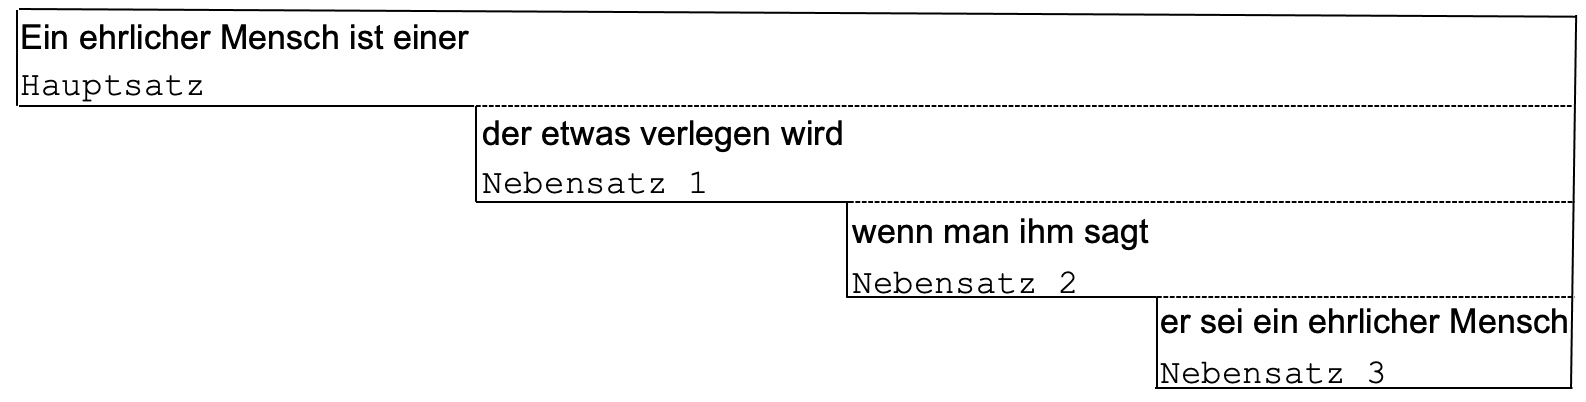
\includegraphics[width=12cm]{figures/Satzbild_Frisch.jpeg}
    %% Abbildung 



\noindent\resizebox{\textwidth}{!}{
	
	\begin{tabular}{ lll }
	
		\hline
		\multicolumn{1}{ | l}{} &&\multicolumn{1}{ l | }{\makecell[l]{stört den Wanderer \\ \small{\textcolor{gray}{Hauptsatz}}}}  \\ \cline{3-3} \sbdashline{1-2}
		
		\multicolumn{1}{ | l }{\makecell[l]{Dass die Leute den Wald verschmutzen \\ \small{\textcolor{gray}{Nebensatz 1}}}} & \multicolumn{1}{ l | }{} & \\ \cline{1-1} \sbdashline{2-2}
		
		& \multicolumn{1}{ | l | }{\makecell[l]{indem sie ihren Müll abladen \\ \small{\textcolor{gray}{Nebensatz 2}}}} & \\ \cline{2-2} 
		
	
	\end{tabular}
}





    \caption{Satzbild zu Satz (\ref{ex:NeSa_Gefüge})}
    \label{Abb:Satzbild}
\end{figure}
 
Der gesamte Satz ist ein Hauptsatz. Hierfür steht die obere durchgezogene Linie. Auf der Hauptsatzebene steht das Hauptsatzgerüst \textit{stört den Wanderer}. Dieser Teilsatz ist unterstrichen. Der Hauptsatz geht jedoch weiter, wofür die gestrichelte Linie steht. Die Nebensätze sind direkt und indirekt eingebettete Bestandteile des Hauptsatzes. Eine Hierarchieebene unter dem Hauptsatzgerüst steht das Nebensatzgerüst von Nebensatz 1 \textit{dass die Leute den Wald verschmutzen}. Der Nebensatz 2 \textit{indem sie ihren Müll abladen} ist ein eingebetteter Bestandteil von Nebensatz 1. Deshalb steht er wieder eine Ebene tiefer. Die gestrichelten Linien symbolisieren die jeweilige Einbettung in die höhere Ebene. Der Nebensatz 2 ist nicht direkt in den Hauptsatz eingebettet, sondern indirekt über Nebensatz 1.    

Bevor es um einzelne Satzglieder geht, ist ihre Abgrenzung von Attributen, die Teile von Satzgliedern sind, wesentlich. Denn \gqq{[d]ie Satzgliedanalyse}, so \citet[80]{Welke2007}, \gqq{steht und fällt mit der Unterscheidung} zwischen Satzgliedern und Attributen. Um diese geht es in dem folgenden Abschnitt~\ref{section:SatzgliederundAttribute}. Zuvor wollen wir jedoch, wie angekündigt, in dem folgenden Exkurs auf den Satzbegriff zurückkommen.

\begin{Exkurs}{Sätze und Nichtsätze?}\label{Exkurs:Satz_Nichtsatz}

Der Satzbegriff, mit dem wir im Rahmen der Satzgliedanalyse arbeiten, ist mindestens an das Vorhandensein eines Verbs als Prädikat gebunden. Er ist also formbezogen. Die von ihm abhängigen Ergänzungen erhalten ihre Form und Funktion erst in ihrer jeweiligen Beziehung zum Prädikat. Ohne Prädikat gibt es keine Satzgliedfunktionen wie Subjekt (vom Prädikat) oder Objekt (vom Prädikat). 

In der Einführung ins Kapitel~\ref{chapter:Feldermodell} haben wir die zentralen sprachlichen Handlungen aufgeführt, die wir mithilfe von Verberst- und Verbzweitsätzen vollziehen (vgl. \textit{Illokution} in Definition~\ref{Def_Illokution}). Auch bestimmte Verbletztsätze verfügen über illokutives Potenzial, dessen wir uns beim selbständigen Gebrauch bedienen: \textit{Dass du mir pünktlich kommst!} Nun gibt es aber auch Äußerungen, die wir wie Sätze gebrauchen, ohne dass sie ein Prädikat enthalten. So verstehen wir (\ref{ea:Landleben}) als Behauptung, (\ref{ex:jetzt_ins_Freiland?}) als Frage und (\ref{ex:jetzt_ins_Moma!}) als Aufforderung. Ebenso denke man an Ausrufe wie \textit{um Himmels willen} in (\ref{ex:himmels_Willen}) und sogenannte Satzäquivalente wie \textit{doch} in (\ref{ex:doch}).

\ea \label{ea:KME}
\ea \label{ea:Landleben} Landleben auf der Potsdamer Straße – mit Ziegen aus dem Öko-Dorf.\footnote{Berliner Zeitung, 19.09.2005.}
\ex \label{ex:jetzt_ins_Freiland?} Jetzt ins Freiland? Mit mir nicht.\footnote{Berliner Zeitung, 06.03.1998.}
\ex \label{ex:jetzt_ins_Moma!} Jetzt ins MoMa! Die Wartezeit beträgt weniger als 45 Minuten.\footnote{Berliner Zeitung, 08.07.2004.}
\ex \label{ex:himmels_Willen} Sie sind ein Fan? Um Himmels willen. Ich gehöre nicht zur Zielgruppe dieser Sendung.\footnote{Berliner Zeitung, 03.03.2003.}
\ex\label{ex:doch} Oder hat sich in der Zwischenzeit nichts geändert? Doch.\footnote{Berliner Zeitung, 29.04.2005.}
\z 
\z  

Vor unserem formbezogenen Hintergrund handelt es sich bei den Äußerungen in (\ref{ea:KME}) nicht um Sätze, sondern um \textit{kommunikative Minimaleinheiten}, wie \citet[86]{ZifHoffStr1997} solche Äußerungen bezeichnen: \gqq{Mit kommunikativen Minimaleinheiten können sprachliche Handlungen vollzogen werden. Der Satz hingegen ist im Rahmen dieser Grammatik eine formbezogen bestimmte Einheit. Sätze enthalten ein finites Verb [\ldots]}. 

\citet[320--321]{Hentschel_Weydt2021} machen darauf aufmerksam, dass auch Äußerungen ohne finites Verb bestimmten Stellungsregeln folgen müssen und dass solche im Rahmen des formbezogenen Ansatzes \textit{nicht-Sätze} in vielen Kontexten viel angemessener sind als die entsprechenden Äußerungen mit einem finiten Verb. Deshalb definieren sie den Satz nach dem Kriterium der syntaktischen Selbständigkeit. Hier lässt sich mit \citet[119]{Engel2009} kritisch nach der Bedeutung von Selbständigkeit fragen: Wie selbständig ist ein Satz, der nur in sehr bestimmten, pragmatisch definierten Situationen zulässig und verständlich ist? Aufgrund der Stellungsregularitäten, die \citet[44]{Musan2021_SGA} auf ein mitverstandenes, aber ausgelassenes Prädikat zurückführt (vgl. \textit{Koordinationsellipse} im Abschnitt~\ref{subsection:SatzgefügeSatzreihe}), bezeichnet sie auch prädikatslose Äußerungen wie in (\ref{ea:KME}) als Sätze. Aufgrund der hier angerissenen Definitionsprobleme gibt \citet[77]{Rothstein2023Syntax} die wohl weiteste Definition von Satz als \gqq{grammatisch vollständige Verbindung mehrerer Konstituenten (wobei sogenannte Einwortsätze, z. B. Ja!, aus nur einer Konstituente bestehen können).}  

Für \citet[70--71]{Welke2005Temp} liegt das Problem in der Definitionsmethode. Anstatt nach \textit{einem} Merkmal zu suchen, das alle Mitglieder einer Kategorie auszeichnet und von anderen Kategorien abgrenzt, plädiert er für eine prototypische Definition: Nicht allen Kategoriemitgliedern kommt dasselbe Merkmal als Invariante zu. Sie weisen verschiedene, über den Prototyp miteinander verbundene Merkmale auf. Ein prototypischer Satz verfügt demnach mindestens über ein finites Verb als Prädikat und über ein illokutives Potenzial. Weniger typische Sätze verfügen nur über eines der beiden, vom Prototyp abgeleiteten Merkmale. Viele Nebensätze verfügen nicht über ein illokutives Potential, aber über ein Prädikat. Auch Infinitive und Partizipien können als Prädikat fungieren, wenn auch nur mit eingeschränktem illokutivem Potenzial. Prädikatslose Äußerungen können als weniger typische Sätze über ein illokutives Potenzial verfügen.

Wesentlich ist die Einsicht, dass auch prädikatslose Äußerungen strukturiert und funktional sind. Hierauf weist besonders \citet[170]{Agel2017} hin, der den prädikatshaltigen Sätzen als Szenario-Ausdruck prädikatslose Nichtsätze als Impressio-Ausdruck komplementär gegenüberstellt: Es handelt sich um \gqq{zwei Grundtypen (einzelsprachlichen) darstellungsfunktionalen Agierens}. Bei Szenario-Ausdrücken bekommen die verbalen Ergänzungen -- anders als die autonom kodierenden Angaben (vgl. Abschnitt~\ref{subsubsection:TestINSP}) -- ihre Werte vom Prädikat zugewiesen. Bei Impressio-Ausdrücken müssen wir den nicht autonom kodierenden Formen, so \citet[170]{Agel2017}, \gqq{auf der Grundlage von satzhaften Analogieerfahrungen und Inferenzen auf der Basis der internen Formen und deren semantischen Beziehungen zueinander} semantische Werte zuweisen, ohne dass diese von einem Prädikat aus berechenbar wären.\footnote{Im Rahmen der grammatischen Textanalyse schlägt \citet[175--191]{Agel2017} eine sehr feine Binnendifferenzierung unter den Nichtsätzen vor, auf die wir nicht weiter eingehen.} Sehen wir uns diesbezüglich in (\ref{ea:Tadellöser}) prädikatslose Äußerungen auf den ersten Seiten des Romans \textit{Tadellöser und Wolff} von Walter Kempowski an. Der Protagonist erzählt den Umzug in eine neue Wohnung.

\ea \label{ea:Tadellöser}
\ea \label{ea:Tadellöser1} Morgens hatten wir noch in der alten Wohnung auf grauen Packerkisten gehockt und Kaffee getrunken (gehört das uns, was da drin ist?). Helle Felder auf den nachgedunkelten Tapeten.\footnote{Walter Kempowski: \textit{Tadellöser und Wolff}. München: Penguin 2016 [1979], S. 1.}
\ex \label{ex:Tadellöser2} Ich teilte mit meinem Bruder Robert das Zimmer. Sechs
Jahre älter als ich. Das blonde Haar stark gewellt, wie die Wogen des Sees Genezareth, in der Bilderbibel, auf denen Jesus wandelt.\footnote{Walter Kempowski: \textit{Tadellöser und Wolff}. München: Penguin 2016 [1979], S. 11.}
\ex \label{ex:Tadellöser3} Mein Vater kaufte sich ein neues Rad. Das alte, mit Dorn
zum Hintenaufsteigen, war verrostet. Dazu einen Kleppermantel, dessen Schöße hochknöpfbar waren.\footnote{Walter Kempowski: \textit{Tadellöser und Wolff}. München: Penguin 2016 [1979], S. 14.}
\z 
\z 

In (\ref{ea:Tadellöser1}) müssen wir eine formal nicht angewiesene Beziehung zwischen der Wortgruppe \textit{Helle Felder auf den nachgedunkelten Tapeten} und dem Vortext herstellen. Da wir diese Wortgruppe nicht direkt in den Vortext einbauen können, interpretieren wir sie als Objekt in einem bekannten und hier plausiblen Existenzausdruck: \textit{Es gab helle Felder auf den nachgedunkelten Tapeten}. Möglich und nicht weniger plausibel wäre auch die Interpretation als Subjekt einer Verortungskonstruktion, die durch die autonom kodierende Wortgruppe \textit{auf den nachgedunkelten Tapeten} motiviert ist: \textit{Helle Flecken befanden sich auf den nachgedunkelten Tapeten}.

In (\ref{ex:Tadellöser2}) interpretieren wir die Wortgruppe \textit{Sechs Jahre älter als ich} als eine Eigenschaft, die dem Bruder Robert zugeschrieben wird. Hierfür nutzen wir das eingeübte prädikative Muster mit dem Verb \textit{sein} und ergänzen den Bruder als Subjekt: \textit{Mein Bruder Robert war/ist sechs Jahre älter als ich}. Auch der nächsten Wortgruppe \textit{das blonde Haar stark gewellt, wie die Wogen des Sees Genezareth, in der Bilderbibel, auf denen Jesus wandelt} müssen wir zur Interpretation einen Wert zuweisen, den sie in Ermangelung eines Hauptprädikats formal nicht zugewiesen bekommt. Wir verstehen sie als Objekt zum Prädikat \textit{haben} oder \textit{tragen} und ergänzen wieder das dazugehörige Subjekt: \textit{Mein Bruder Robert hatte das blonde Haar stark gewellt \ldots} oder \textit{Mein Bruder Robert trug das blonde Haar stark gewellt \ldots}. Ebenso möglich wäre es, die formal nicht angewiesene Stellung der Wortgruppe analog zu dem vorherigen Fall im Rahmen einer Eigenschaftszuweisung zu verstehen: \textit{Sein blondes Haar war stark gewellt \ldots}. 

In (\ref{ex:Tadellöser3}) haben wir es bei \textit{Dazu einen Kleppermantel, dessen Schöße hochknöpfbar waren} mit einer NP im Akkusativ zu tun. Da es kein Prädikat gibt, können wir der Wortgruppe nicht den erwartbaren Wert Akkusativobjekt zuweisen. Wir orientieren uns am Vortext und interpretieren diese Wortgruppe als Akkusativobjekt zum Prädikat \textit{kaufte} im ersten Satz.   

In den Textpassagen in (\ref{ea:Tadellöser}) sind wir auf Formen gestoßen, deren syntaktische und semantische Funktion formal nicht durch ein übergeordnetes Prädikat bestimmt ist. Wir haben sie in Analogie zu uns bekannten Sätzen und im Rahmen der vorangehenden Sätze assoziativ interpretiert. Eben hierin liegt auch der Reiz solcher prädikatslosen Äußerungen gegenüber Szenario-Ausdrücken mit Prädikat. Der Leser bzw. die Leserin muss ohne formale Anweisung die Formen in mögliche (früher schon erfahrene) prädikative Strukturen und in den laufenden Text im Sinne syntaktisch-semantischer Werte einbetten. Beim Lesen entsteht aus formalen Reihungen, aus Erinnerungsfetzen und Eindrücken (Impressionen) etwas Zusammenhängendes.

\end{Exkurs}



\section{Attribute als Teile von Satzgliedern}\label{section:SatzgliederundAttribute}


Attribute\is{Attribut} hängen von nicht-verbalen Bezugswörtern als Köpfen ab und stehen somit nur in mittelbarer Beziehung zum Prädikat.\footnote{Diese weite Bestimmung des Attributbegriffs folgt \citet[110]{Elst_Habermann_SynAn}, \citet[502]{HelbigBuscha}, \citet[81]{Welke2007}, \citet[152]{OehlSeiler2013} und \citet[698]{Agel2017}. \citet[259]{Eisenberg2020_Satz} geht von einem engen Attributbegriff als Prototyp aus, erweitert ihn aber. \citet[351]{Schaefer2018_3Aufl} schränkt, wie das traditionell üblich war, den Attributbegriff auf Konstituenten der Nominalphrase ein. Einen Überblick zur Begriffsgeschichte geben \citet[307--309]{FuhrhopThierrof2005}, speziell zur jüngeren Abgrenzungsproblematik \citet[231--233]{Engel2011Attribut}.} Den Prototyp des Attributs bilden die im Abschnitt~\ref{section:NP} aufgezeigten Möglichkeiten, einen nominalen Kopf insbesondere\is{Attribut!Typen} durch Adjektivphrasen, NPs im Genitiv, durch PPs und Relativsätze auszubauen. Deshalb spricht man von Adjektivattributen (\ref{ea:Adjektivattribut}), Genitivattributen (\ref{ex:Genitivattribut}), Präpositionalattributen (\ref{ex:PPAttribut}) und Relativsatzattributen (\ref{ex:Relativsatzattribut}). 

\ea \label{ea:NAttribute}
\ea \label{ea:Adjektivattribut} Die \textit{große} Frau tanzt.
\ex \label{ex:Genitivattribut} Die Frau \textit{meines Bruders} tanzt.
\ex \label{ex:PPAttribut} Die Frau \textit{mit dem Hut} tanzt.
\ex \label{ex:Relativsatzattribut} Die Frau, \textit{die einen Hut trägt}, tanzt.
\z 
\z 

Durch Attribute wird diejenige Entität, die von einer NP bezeichnet wird, ihr Referent, genauer charakterisiert, oder die Menge der möglichen Referenten wird eingeschränkt. So wird in (\ref{ea:Adjektivattribut}) entweder die Person, die wir mit \textit{die Frau} bezeichnen, näher beschrieben oder aber, wenn mehrere Frauen in Frage kommen, klargestellt, um welche Frau es geht, hier um die große und nicht um die kleine.  

Attribute können nicht alleine im Vorfeld (vgl. Abschnitt~\ref{subsection:Vorfeld}) stehen. Sie können nur zusammen mit ihrem Kopf und der von diesem gebildeten Phrase im Vorfeld stehen, wenn diese Phrase ein Satzglied ist. Alleine sind sie nicht vorfeldfähig (\ref{ea:NAttributeTests}), zumindest nicht bei gleicher Bedeutung. Hierfür steht die Raute bei (\ref{ex:PPAttribut_pron}) im Vergleich zu (\ref{ex:PPAttribut}). 

\ea \label{ea:NAttributeTests}
\ea  [*] {\textit{Große} tanzt die Frau.}\label{ea:Adjektivattribut_top}
\ex [*] {\textit{Meines Bruders} tanzt die Frau.}\label{ex:Genitivattribut_erfragbar}
\ex [\#] {\textit{Mit dem Hut} tanzt die Frau.}\label{ex:PPAttribut_pron}
\ex [*] {\textit{Die einen Hut trägt,} tanzt die Frau.}\label{ex:Relsatz_VF}
\z 
\z 

In Bezug auf die Beispiele in (\ref{ea:NAttribute}) mag die Frage aufkommen, warum wir die Artikel nicht zu den Attributen zählen. Auch sie hängen vom Substantiv und nicht vom Verb ab.\footnote{\citet[235]{Engel2011Attribut} zählt aufgrund der Abhängigkeit vom Substantiv auch Artikel zu den Attributen. Die \citet[441, §722]{Duden2022} zählt nur die Possessivartikel wie \textit{sein} zu den Attributen, da diese Artikel und gleichzeitig possessive Attribute seien: \textit{das Haus von Paul}, \textit{Pauls Haus} und  \textit{sein Haus}. Für \citet[321--322]{FuhrhopThierrof2005} ist das wesentliche Argument gegen den Attributstatus von Artikeln, dass diese ausschließlich als Funktionsträger in Nominalphrasen vorkommen und dabei selbst nicht durch Attribute erweiterbar sind.} Wir zählen Artikel grundsätzlich nicht zu den Attributen. Artikel sind obligatorische funktionale Bestandteile von Nominalphrasen (vgl. Abschnitt~\ref{section:NP}). Sie zeigen deren grammatische Merkmale an und setzen die Bedeutung des Substantivs zu konkreten Individuen bzw. Entitäten in Beziehung (Determination). Attribute sind fakultativ und reichern die Bedeutung des Substantivs bzw. der Nominalphrase an (Modifikation). Funktional kann es durchaus zu Überschneidungen zwischen Artikeln und Attributen kommen.

Wir haben gesagt, dass Attribute nur zusammen mit ihrem Bezugswort im Vorfeld stehen können. Deshalb ist (\ref{ex:Relsatz_VF}) ungrammatisch. Allerdings erscheinen Relativsatzattribute häufig von ihrem im Mittelfeld (vgl. Abschnitt~\ref{subsection:Mittelfeld}) stehenden Bezugswort getrennt, indem sie wie in (\ref{ea:RelSatzNF}) im Nachfeld (vgl. Abschnitt~\ref{subsection:Nachfeld}) stehen.

\ea \label{ea:RelSatzNF} Er hat die Frau gegrüßt, die einen Hut trägt.
\z 


Auch bestimmte andere Attribute können getrennt von ihrem Bezugswort stehen. Entweder steht das Bezugswort wie in (\ref{ea:Wer_von_Split}) allein im Vorfeld und das Attribut steht im Mittelfeld oder das Attribut steht wie in (\ref{ex:PP_Attribut_Split}) allein im Vorfeld und das Bezugswort steht im Mittelfeld.\footnote{Bei den Stellungen zwischen Kopf und \textit{von}-Attribut in (\ref{ea:Attribut_Split}) handelt es sich um eine Element-Menge-Trennung. Andere sogenannte Splitkonstruktionen bildet man mit \textit{was für}, \textit{w- alles}, \textit{w- an} und \textit{w-} mit substantiviertem Adjektiv: \textit{Was hat er für ein Problem?}; \textit{Wer hat alles zugestimmt?}; \textit{Was gibt es noch an Problemen?}; \textit{Was gibt es Neues?} Cf. \citet[145--146]{Pafel1995}.}

\largerpage
\ea \label{ea:Attribut_Split}
\ea \label{ea:Wer_von_Split} Wer hat \textit{von den Abgeordneten} gegen den Antrag gestimmt?
\ex \label{ex:PP_Attribut_Split} \textit{Von den Abgeordneten} hat eine Mehrheit gegen den Antrag gestimmt.
\z 
\z   

Dennoch handelt es sich bei \textit{von den Abgeordneten} in (\ref{ea:Wer_von_Split}) um ein Attribut von \textit{wer} und in (\ref{ex:PP_Attribut_Split}) um ein Attribut von \textit{Mehrheit}. Das Attribut schränkt die Menge der unter \textit{wer} bzw. \textit{eine Mehrheit} fallenden Personen ein. Das Attribut steht nicht in direkter Beziehung zum Prädikat: *\textit{Von den Abgeordneten hat gegen den Antrag gestimmt}. In beiden Fällen können das Bezugswort und das Attribut zusammen das Vorfeld besetzen (\ref{ea:Attribut_kein_Split}).

\ea \label{ea:Attribut_kein_Split}
\ea \label{ea:Wer_von_PP} Wer \textit{von den Abgeordneten} hat gegen den Antrag gestimmt?
\ex \label{ex:Mehrheit_von_PP} Eine Mehrheit \textit{von den Abgeordneten} hat gegen den Antrag gestimmt.
\z 
\z   


\begin{Definition}{Attribut}
    
\noindent Attribute sind Wörter oder Wortgruppen eines Satzes, die keine direkte Beziehung zum Prädikat haben und die folglich keine Satzglieder sind. Attribute sind fakultative Bestandteile von Satzgliedern. Der Prototyp hängt vom Kopf einer NP ab und beschreibt deren Referenten näher oder grenzt den Referenzbereich ein.    
\end{Definition}




Als besondere\is{Attribut} Attribute betrachten wir die im Exkurs~\ref{subsection:Apposition} diskutierten lockeren (\ref{ea:Attr_lockere_Apposition}) und engen Appositionen (\ref{ex:Attr_engeApposition}). Hierzu gehören auch die Stoff- bzw. Inhaltsangaben als Attribut zu Mengen- und Maßbezeichnungen (\ref{ex:Maß_Inhalt}). 

\ea \label{ea:NAttribut_Apposition}
\ea \label{ea:Attr_lockere_Apposition} Berlin, \textit{die Bundeshauptstadt}, ist Deutschlands größte Stadt.
\ex \label{ex:Attr_engeApposition} Die Bundeshauptstadt \textit{Berlin} ist Deutschlands größte Stadt.
\ex \label{ex:Maß_Inhalt} Zwei Flaschen \textit{Saft} sind noch da.
\z 
\z 

Da wir einen weiten\is{Attribut} Attributbegriff ansetzen, sprechen wir auch beim Ausbau von APs (\ref{ea:A_Attribut}) und PPs (\ref{ex:P_Attribut}) von Attributen. 

\ea \label{ea:XAttribute}
\ea \label{ea:A_Attribut} Die \textit{auf ihren Enkel} stolze Oma lacht.
\ex \label{ex:P_Attribut} Sie traf ihn \textit{kurz} vor Mitternacht.
\z 
\z 

Die PP \textit{auf ihren Enkel} in (\ref{ea:A_Attribut}) ist eine Ergänzung des Adjektivs \textit{stolze}. Auf der Ebene des Satzes handelt es sich bei \textit{auf ihren Enkel} um ein Attribut von \textit{stolze}. Beide zusammen sind als AP Attribut zu \textit{Oma}.\footnote{\citet[68]{Musan2021_SGA} bezeichnet auch die Ergänzungen von Adjektiven als Objekte. Die PP \textit{auf ihren Enkel} in (\ref{ea:A_Attribut}) wäre demzufolge ein Präpositionalobjekt zu \textit{stolze}. Wir reservieren den Objektbegriff für die Ebene der Satzglieder. Will man differenzieren zwischen valenziell verankerten Attributen und frei hinzufügbaren, so kann man wie \citet[493]{HelbigBuscha} von valenzbedingten und valenzunabhängigen Attributen sprechen.} Die ganze NP \textit{die auf ihren Enkel stolze Oma} ist Subjekt von \textit{lacht}. In (\ref{ex:P_Attribut}) ist \textit{kurz} ein Adjektivattribut der PP \textit{vor Mitternacht}. Beide zusammen bilden als komplexe PP \textit{kurz vor Mitternacht} ein Satzglied, das als temporales Adverbial fungiert.  

Am Beispiel\is{Attribut!komplex} der NP (vgl. Abschnitt~\ref{section:NP}) und der AP (vgl. Abschnitt~\ref{section:AP}) haben wir Folgendes gesehen: Mehr als ein Attribut kann sich auf einen Kopf beziehen. Das hat Auswirkungen auf die Kommasetzung (\textit{kluge, unterhaltsame Bücher} versus \textit{spannende französische Bücher}). Adjektivattribute können also sehr komplex sein, da sie intern wiederum Phrasen bilden. Eine besondere Komplexität von Attributen kann dadurch entstehen, wenn wir VPs wie \textit{ein Haus bauen} nominalisieren\is{Substantivierung}, also in eine NP wie \textit{der Bau eines Hauses} umwandeln.

In Kapitel \ref{chap:Konstituenz} haben wir gezeigt, dass der Ausbau des Verbkopfes zum Satz analog beschreibbar ist wie der Ausbau nominaler Köpfe zur NP. Mit dem\is{Attribut} Attributbegriff trennen wir beide Ausbau-Ebenen.\footnote{Viele Grammatikmodelle basieren auf der grundlegenden Unterscheidung zwischen Köpfen auf der einen Seite und Ergänzungen (Argumenten) sowie Angaben (Adjunkten) auf der anderen Seite. Ein Äquivalent zum Attributbegriff gibt es nicht.} Für den Attributbegriff und damit die Trennung der verbalen von allen anderen Ebenen sprechen formale und funktionale Gründe. \citet[46]{Eichinger1995} schreibt, dass es sich bei verbaler und nominaler Ebene um \gqq{funktionale Kategorisierungsstufen eigener Art} handele. \citet[254]{Welke2011} hält die substantivische und verbale Konstruktion für \gqq{grundverschieden}.

In\is{Satzglied!versus Attribut} der verbalen Konstruktion, also auf Ebene der Satzglieder, spielen NPs im Nominativ, im Akkusativ und im Dativ eine primäre Rolle für die Kodierung von Subjekt, Akkusativobjekt und Dativobjekt.\footnote{Im Bereich der verbalen Ergänzungen haben wir den Genitiv in Abschnitt~\ref{subsubsection:TestFOSP} als Relikt beschrieben.} Diese sättigen die Valenzanforderungen des Prädikats. Das Prädikat weist den vom Subjekt und von den Objekten Bezeichneten Rollen zu, was in Abschnitt~\ref{subsubsection:TestINSP} als\is{Prädikation} Prädikation beschrieben wurde. Auf dieser Grundlage bilden wir Sätze. Mit Sätzen handeln wir, indem wir \zB etwas aussagen, befehlen oder fragen. 

In der nominalen Konstruktion, also auf\is{Attribut!komplex} Attributebene, spielen Adjektivattribute und NPs im Genitiv die zentrale Rolle. Diese sättigen typischerweise keine valenziellen Forderungen. Daher zeichnet sich die nominale Attribution (im Vergleich zum Verbalbereich) durch große Variation aus.\footnote{Cf. \citet[318]{FuhrhopThierrof2005}.} Originäre (nicht vom Verb oder Adjektiv abgeleitete) Nomen prädizieren typischerweise nicht über den Attributen. Mit NPs allein treffen wir keine expliziten Aussagen, erteilen keine expliziten Befehle und stellen keine expliziten Fragen. Hierzu muss die NP Teil einer finiten VP werden. Durch Attribute erweiterte NPs sind als dichte Informationsverpackungen ein Merkmal der Bildungssprache.\footnote{Seit dem 16. Jahrhundert wird die NP durch Attribution immer komplexer. Das führt letztlich zur Entwicklung des für die Bildungssprache typischen Nominalstils. Cf. \citet[36--38]{Admoni1973}, \citet[6]{CziczaHenningetal2012}.} Ihre korrekte Bildung und ihr Verständnis setzen voraus, den Kopf als Bezugswort zu erkennen und die Bedeutungen der Attribute schrittweise auf das vom Bezugswort Bezeichnete zu übertragen. Wir illustrieren dies anhand der eingeklammerten komplexen NP in (\ref{ea:komplexeNPAttribut}), die wir in (\ref{ex:expl1}), (\ref{ex:expl2}) und (\ref{ex:expl3}) in explizite Prädikationen überführen. Das Präpositionalattribut \textit{in einer demokratischen Gesellschaft} kann auch wie in (\ref{ex:expl4}) als Attribut auf den nominalen Kern \textit{Grundlage} bezogen werden.  

\ea \label{ea:Attributbeispiel}
\ea \label{ea:komplexeNPAttribut} Sie (die Medienbildung, M.F.) ist [...] eine essentielle Voraussetzung für Ausbildungs- und Studierfähigkeit und [Grundlage lebenslangen Lernens in einer demokratischen Gesellschaft].\footnote{Senatsverwaltung für Bildung, Jugend und Familie: Rahmenlehrplan 1--10 kompakt. Themen und Inhalte des Berliner Unterrichts im Überblick. 2017. \url{https://www.berlin.de/sen/bildung/unterricht/faecher-rahmenlehrplaene/rahmenlehrplaene/} (08.05.19).}
\ex \label{ex:expl1} Die Grundlage betrifft das Lernen.
\ex \label{ex:expl2} Das Lernen geschieht lebenslang.
\ex \label{ex:expl3} Das lebenslange Lernen findet in einer demokratischen Gesellschaft statt.
\ex \label{ex:expl4} Die Grundlage betrifft das lebenslange Lernen und liegt in einer demokratischen Gesellschaft.
\z 
\z 

Aber es gibt auch Gemeinsamkeiten zwischen der Ebene der\is{Satzglied!versus Attribut} Satzglieder und der\is{Attribut!versus Satzglied} Attribute. Eine Gemeinsamkeit betrifft die Abhängigkeitsrelation. Die Satzglieder hängen vom Prädikat ab und die Attribute von einem nominalen Kopf. Wenn wir im Bild der Matroschka bleiben, dann sind die Attribute kleinere Matroschkas, die in den größeren Satzglied-Matroschkas stecken. Formal können sowohl Satzglieder als auch Attribute durch PPs realisiert werden, wie einführend anhand der doppeldeutigen Überschrift \textit{Polizei jagt Verbrecher mit Oldtimer} illustriert wurde. Analog dazu können wir die kursiv gedruckte PP \textit{durch die Polizei} in (\ref{ea:durchPolizei}) als Satzglied\is{Satzglied!versus Attribut} oder als Attribut\is{Attribut!versus Satzglied} interpretieren.

\ea \label{ea:durchPolizei} Dieser Bereich wird zur Verhütung von Straftaten \textit{durch die Polizei} videoüberwacht.\footnote{\url{https://de.wikipedia.org/wiki/Mehrdeutigkeit} (02.04.18).} 
\z

Dem\is{Ambiguität!syntaktisch} primären Verständnis zufolge ist die PP als Satzglied direkt dem Prädikat untergeordnet: \textit{durch die Polizei videoüberwacht werden}. Sie besteht die in Kapitel \ref{chap:Konstituenz} vorgestellten Satzgliedtests. Sie ist durch ein Pronomen erfragbar (\ref{ea:durchdiePolizeiErfragbar}) und voranstellbar (\ref{ex:durchdiePolizeiVoranstellbar}). 

\ea \label{ea:SGTestdurchdiePolizei}
\ea \label{ea:durchdiePolizeiErfragbar} \textit{Durch wen} wird dieser Bereich zur Verhütung von Straftaten videoüberwacht?
\ex \label{ex:durchdiePolizeiVoranstellbar} \textit{Durch die Polizei} wird dieser Bereich zur Verhütung von Straftaten videoüberwacht. 
\z 
\z 

Möglich (wenn auch unwahrscheinlich) ist jedoch auch die Einbettung der PP unter \textit{Straftaten}, ihr Gebrauch also als Attribut in \textit{Straftaten durch die Polizei} mit der Bedeutung \gq{Straftaten, die durch die Polizei verübt werden}. In diesem Fall besteht die PP \textit{durch die Polizei} nicht die Satzgliedtests. Sie ist nicht alleine erfragbar und voranstellbar nur innerhalb des Satzglieds, dessen Teil sie ist  (\ref{ea:durchdiePolizeiAttribut}).

\ea \label{ea:durchdiePolizeiAttribut} \textit{Zur Verhütung von Straftaten durch die Polizei} wird dieser Bereich videoüberwacht.
\z 

Trotz unterschiedlicher Einbettung, einmal als\is{Satzglied!versus Attribut} Satzglied und einmal als\is{Attribut!versus Satzglied} Attribut, drückt die PP auf ähnliche Weise die verursachende Entität aus. 

Auch Adverbien können neben ihrem primären Gebrauch als Satzglied (\ref{ea:AdvSG}) postnominal als Attribut wie in (\ref{ex:AdvAttribut}) gebraucht werden. 

\ea \label{ea:AdvAttributSatzglied}
\ea \label{ea:AdvSG} Der Film lief \textit{gestern}.
\ex \label{ex:AdvAttribut} Der Film \textit{gestern} hat viele begeistert.
\z 
\z 

Ein\is{Satzglied!zum Attribut} und\is{Attribut!aus Satzglied} derselben Form wie der PP in (\ref{ea:durchPolizei}) oder der Adverbphrase in (\ref{ea:AdvAttributSatzglied}) kommt je nach Bezugsgröße eine andere syntaktische Funktion zu. Die Funktion eines sprachlichen Ausdrucks ist nur in Beziehung zu einem anderen Ausdruck zu bestimmen.    

\citet[35, 55]{Agel2017} bezeichnet die Identität auf verschiedenen Funktionsebenen als \gqq{Recycling} und schreibt: \gqq{Analoge semantische Werte [...] werden vertikal -- hierarchisch -- durch die funktionalen Ebenen grammatisch \gq{durchgereicht}}. Hierbei handelt es sich, so \citet[751]{Agel2017}, um \gqq{ein elementares \textit{funktionales} Merkmal des grammatischen Systems}. Neues wird weitgehend analog zu Bestehendem (und daher ökonomisch) nachgebildet.\footnote{Cf. \citet[295]{Langacker1991}.} Lokale und temporale Attribute wie \textit{dort} und \textit{gestern} in \textit{der Baum dort} und \textit{der Film gestern} sind durch Analogie zur Adverbialebene motiviert, wie in \textit{der Baum steht dort} und \textit{der Film lief gestern}. Andere Attribute wie \textit{auf gutes Wetter} in \textit{die Hoffnung auf gutes Wetter} sind durch Analogie zur Objektebene motiviert, wie in \textit{sie hoffen auf gutes Wetter}.

Dieses \textit{Recycling} zeigt sich besonders bei der Ableitung von\is{Nominalisierung} Nomen aus Verben (deverbale Nomen). Da der Nominalstil typisch für die Schul- und Bildungssprache\footnote{Cf. \citet[489--490]{GogolinDuarte2016}.} ist, gehen wir etwas genauer darauf ein. Wenn das Verb eine Präposition regiert wie \textit{auf etwas hoffen} (\ref{ea:hoffenauf}), so erbt das abgeleitete Nomen \textit{Hoffnung} diese Präposition (\ref{ex:Hoffnungauf}). Die Nominativ-NP in Subjektfunktion kann bei Nominalisierung als Genitiv-NP, bei Eigennamen wie \textit{Paul} in (\ref{ea:hoffenauf}) postnominal, ausgedrückt werden.

\ea \label{ea:Nominalisierung}
\ea \label{ea:hoffenauf} Paul hofft \textit{auf gutes Wetter}.
\ex \label{ex:Hoffnungauf} Pauls Hoffnung \textit{auf gutes Wetter}
\z 
\z 

Aus dem Präpositionalobjekt in (\ref{ea:hoffenauf}) ist in (\ref{ex:Hoffnungauf}) ein Präpositionalattribut\is{Attribut!versus Satzglied} geworden und aus dem Nominativsubjekt ein Genitivattribut.  Während in (\ref{ea:hoffenauf}) explizit eine Aussage gemacht wird, ist dies in (\ref{ex:Hoffnungauf}) nicht, oder nur implizit der Fall. Aus dem Verb ist ein Nomen geworden. Die aus dem Nomen gebildete NP kann als Satzglied einem anderen Prädikat (\ref{ea:NPalsneuesObjekt}) oder als Attribut einem Nomen (\ref{ex:NPalsAttribut}) untergeordnet werden. So können wir viele Informationen kompakt auf der Nominalebene unterbringen. 

\ea \label{ea:Nominalisierungsdichte}
\ea \label{ea:NPalsneuesObjekt} Anna spottet über \textit{Pauls Hoffnung auf gutes Wetter}.
\ex \label{ex:NPalsAttribut} \textit{Annas Spott über Pauls Hoffnung auf gutes Wetter} ist allen bekannt.
\z 
\z 

Analog zur Umfunktionierung der PP in (\ref{ea:Nominalisierungsdichte}) können auch Nebensätze von Satzgliedern (\ref{ea:NeSaObj}) zu\is{Attribut!Nebensatz} Attributen (\ref{ea:NeSaAttr}) umfunktioniert werden. 

\ea \label{ea:NeSaAttrSG}
\ea \label{ea:NeSaObj} Paul hofft, \textit{dass gutes Wetter wird}.
\ex \label{ea:NeSaAttr} Pauls Hoffnung, \textit{dass gutes Wetter wird}
\z 
\z 

Das\is{Satzglied!Recycling} Gleiche gilt für Infinitivgruppen: In (\ref{ea:InfObj}) ist \textit{Anna wiederzusehen} ein Satzglied, in (\ref{ex:InfAttr}) hingegen ein Attribut.

\ea \label{ea:InfAttrSG}
\ea \label{ea:InfObj} Paul hofft, \textit{Anna wiederzusehen}.
\ex \label{ex:InfAttr} Pauls Hoffnung \textit{Anna wiederzusehen}
\z 
\z 


Wenn\is{Nominalisierung} Verben über ein Akkusativobjekt verfügen wie \textit{etwas beantworten}, dann wird dieses bevorzugt als Genitivattribut an das deverbale Nomen vererbt. Das ist insbesondere bei Handlungsverben (vgl. Abschnitt~\ref{subsection:Verbklassen}) der Fall, da das Geschehen auf die Veränderung oder das Hervorbringen der Entität abzielt, die durch das Akkusativobjekt bezeichnet wird. Wenn die Subjekt-NP ein Eigenname ist wie \textit{Paul} in (\ref{ea:VAkkobj}), kann dieser als pränominales Genitivattribut in der NP ausgedrückt werden (\ref{ex:NGenAttr}) oder postnominal mittels einer PP mit \textit{durch} wie in (\ref{ex:durchPP}). 

\ea \label{ea:NominalisierungAkkObj}
\ea \label{ea:VAkkobj} Paul beantwortet die Frage.
\ex \label{ex:NGenAttr} Pauls Beantwortung der Frage
\ex \label{ex:durchPP} die Beantwortung der Frage durch Paul
\z 
\z 

Das Substantiv \textit{Beantwortung} ist der Name für einen Vorgang. Dieser Vorgang lässt sich umschreiben als \gq{etwas wird beantwortet}. Zu jener Vorgangslesart passt es, dass das ursprüngliche Akkusativobjekt nun als Genitivattribut in der NP ausgedrückt wird. Als Genitivattribut verstehen wir \textit{der Frage} nicht als Akkusativobjekt von \textit{beantworten}, sondern als Subjekt des Vorgangsausdrucks \textit{die Frage wird beantwortet}.\footnote{Cf. \citet[48]{Eichinger1995}. \citet[250--313]{Welke2011} analysiert Nominalisierungen ausführlich, insbesondere die Faktoren, die die nominale Lesart wieder zurück in die verbale überführen.}  

Eine ähnliche\is{Satzglied!Recycling} Art von Recycling findet statt, wenn wir ein verbales Partizip als Adjektivattribut eines Nomens verwenden. In (\ref{ex:Partizipialattribut1}) wird das Partizip I \textit{bauende} attributiv gebraucht, in (\ref{ex:Partizipialattribut2}) das Partizip II \textit{gebaute}.  

\ea \label{ea:Partizipienableitung}
\ea \label{ea:Verb} Paul baut für Anna einen Schneemann.
\ex \label{ex:Partizipialattribut1} der für Anna einen Schneemann bauende Paul
\ex \label{ex:Partizipialattribut2} der von Paul für Anna gebaute Schneemann
\z 
\z 

Im Satz\is{Partizip I!attributiv} (\ref{ea:Verb}) wird das Verb \textit{baut} als Prädikat und \textit{Paul} als dessen Subjekt, \textit{einen Schneemann} als Objekt und \textit{für Anna} als Adverbial gebraucht. Mit dem attributiven Gebrauch der Partizipien werden aus bestimmten Satzgliedern Attribute. Das Partizip I (\ref{ex:Partizipialattribut1}) kann bis auf das Subjekt die Valenz des Verbs übernehmen. Aus dem Akkusativobjekt \textit{einen Schneemann} in (\ref{ea:Verb}) wird ein Attribut im Akkusativ (\ref{ex:Partizipialattribut1}). Auch das Adverbial \textit{für Anna} wird direkt als Attribut in die adjektivische Konstruktion übernommen. Das Partizip I drückt die Fortdauer des vom Verb bedeuteten Geschehens aus. Attributiv überträgt es diese Bedeutung als Eigenschaft auf das ursprüngliche Subjekt.

Das Partizip II\is{Partizip II!attributiv} (\ref{ex:Partizipialattribut2}) transitiver telischer Verben (vgl. Abschnitt~\ref{subsection:Verbklassen}) drückt den Nachzustand aus, welchen das Verb impliziert. Wenn \textit{ein Schneemann gebaut wird}, dann impliziert das, dass es als Nachzustand einen \textit{gebauten Schneemann} gibt.\footnote{Zur Bildung und zu Restriktionen des attributiven Gebrauchs von Partizipien vgl. Abschnitt~\ref{subsubsection:MorphKonv}.} 

Das Partizip II wird als\is{Partizip II!attributiv} Attribut mit seiner Nachzustandslesart auf das ursprüngliche verbale Akkusativobjekt übertragen. Das ursprüngliche Subjekt des Verbs \textit{Paul} wird als PP-Attribut an das adjektivische Partizip II vererbt. Das Adverbial \textit{für Anna} wird wie beim Partizip I ohne formale Veränderung als Attribut übernommen. Auch telische intransitive Verben wie \textit{verblühen} implizieren einen Nachzustand. Dieser kann attributiv durch das Partizip II auf den ursprünglichen Vorgangsträger wie \textit{die Blume} in \textit{die Blume verblüht} übertragen werden: \textit{die verblühte Blume}.

Die\is{Attribut!komplex} auf diese Weise komplex gebauten NPs beinhalten nicht mehr die Satzaussage aus (\ref{ea:Verb}) als Behauptung, sondern setzen diese voraus. Die durch Attribution komplexen NPs können nun wieder als Satzglied anderer Prädikate dienen, so in (\ref{ea:PartAttrNPObj}) als Objekt und in (\ref{ex:ea:PartAttrNPSubjekt}) als Subjekt, wodurch eine hohe Informationsdichte auf der Ebene eines Satzes erreicht wird.

\ea \label{ea:PartAttrNP}
\ea \label{ea:PartAttrNPObj} Ich sehe den für Anna einen Schneemann bauenden Paul.
\ex \label{ex:ea:PartAttrNPSubjekt} Der von Paul für Anna gebaute Schneemann gefällt allen.
\z 
\z 



\section{Exemplarische Analyse}\label{section:exemplAnalyse}

Bevor es um einzelne Satzglieder geht, führen wir anhand des folgenden Satzes in (\ref{ea:EisenbergSatz}) eine exemplarische Satzanalyse durch. Die Ergebnisse stellen wir im Tabellenformat dar.

\ea \label{ea:EisenbergSatz} Wir verfügen heute über riesige elektronische Korpora, an denen wir genau sehen können, an welchen Punkten die Journalisten ihren Sprachgebrauch verändert haben.\footnote{Eisenberg, Peter: \textit{Die deutsche Sprache war noch nie so gut in Form wie heute.} Rundfunkinterview mit Dagmar Giersberg. In: Online-Material zum Themenheft Zentralabitur: Deutsche Sprache der Gegenwart. Leipzig: Klett 2009, 7--8. \url{https://www2.klett.de/sixcms/media.php/229/347493_0004.pdf} (03.06.2026).} 
\z 

Der erste Analyseschritt besteht darin, das Prädikat des Hauptsatzes zu finden. Das finite Verb \textit{verfügen} steht an zweiter Stelle und bildet das Prädikat des Hauptsatzes. Das Hauptsatzgerüst besteht aus \textit{wir verfügen heute über riesige elektronische Korpora}. Die beiden Nebensätze sind in den Hauptsatz eingebettet. Wir erkennen sie an der Verbendstellung: \textit{an denen wir genau sehen können} und \textit{an welchen Punkten die Journalisten ihren Sprachgebrauch verändert haben}.

Im zweiten Schritt ermitteln wir, worauf sich die\is{Nebensatz!Einbettung} Nebensätze beziehen bzw. wovon sie abhängen. Der erste Nebensatz bezieht sich auf die NP \textit{riesige elektronische Korpora}. Mit anderen Worten ist er in diese NP des Hauptsatzes eingebettet. Der zweite Nebensatz bezieht sich auf den ersten Nebensatz. Er drückt aus, was man sehen kann. Der zweite ist in den ersten Nebensatz eingebettet. Die Einbettungsebenen stellen wir als Satzbild\is{Satzbild} in Abbildung~\ref{Abb:Satzbild_Korpora} dar.

\begin{figure}
    \centering
    %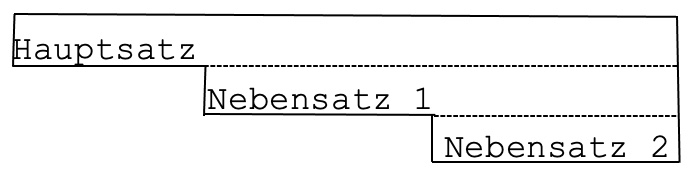
\includegraphics[width=7cm]{figures/Satzbild_Korpora.jpeg}
    %% Abbildung 


\centering{
	\noindent\resizebox{\textwidth}{!}{
		
		\begin{tabular}{ p{4cm} p{4cm} p{4cm} | }
			
			\hline 
			\multicolumn{1}{ | l }{\makecell[l]{\small\textcolor{gray}{Hauptsatz}}} && \\ \cline{1-1} \sbdashline{2-3}
			
			& \multicolumn{1}{ | l }{\makecell[l]{\small\textcolor{gray}{Nebensatz 1}}} &  \\ \cline{2-2} \sbdashline{3-3}
			
			& & \multicolumn{1}{ | l | }{\makecell[l]{\small\textcolor{gray}{Nebensatz 2}}}  \\ \cline{3-3}
			
		\end{tabular}
	}
}




    \caption{Satzbild zu (\ref{ea:EisenbergSatz})}
    \label{Abb:Satzbild_Korpora}
\end{figure}

Die Satzgliedanalyse beginnt auf der Hauptsatzebene. Zuerst muss das Hauptprädikat als hierarchisch oberste Einheit bestimmt werden. In unserem Satz ist \textit{verfügen} das Prädikat in der Lesart von \gq{etwas besitzen und verwenden können}. Nun bestimmen wir die Valenz des Prädikats. Es ist zweiwertig. Die erste Ergänzung wird durch die Nominativ-NP \textit{wir} in Subjektfunktion realisiert. Die zweite Ergänzung wird als PP mit \textit{über} in Funktion eines Präpositionalobjekts ausgedrückt. Wir haben festgestellt, dass der erste Nebensatz in die NP \textit{riesige elektronische Korpora} eingebettet ist. Diese wiederum ist Teil der PP, also: \textit{über riesige elektronische Korpora, an denen wir genau sehen können}. Den zweiten Nebensatz haben wir als Teil des ersten Nebensatzes bestimmt. Die PP ist also äußerst komplex. Mit beiden Nebensätzen zusammen fungiert sie auf der Hauptsatzebene als Präpositionalobjekt des Prädikats \textit{verfügen}. 

Hierfür sprechen auch die Satzgliedtests: Die komplexe PP ist auf oberster Ebene als Ganze pronominalisierbar (\ref{ea:PPdarüber}), erfragbar (\ref{ex:PPworüber}) und voranstellbar (\ref{ex:PPvorangestellt}).

\ea \label{ea:SGTests}
\ea \label{ea:PPdarüber} Wir verfügen heute [darüber].
\ex \label{ex:PPworüber} [Worüber] verfügen wir heute?
\ex \label{ex:PPvorangestellt} [Über riesige elektronische Korpora, an denen wir genau sehen können, an welchen Punkten die Journalisten ihren Schreibgebrauch verändert haben], verfügen wir heute.
\z 
\z 

Neben den primären Satzgliedern Subjekt und Präpositionalobjekt bezieht sich die Adverbphrase \textit{heute} ebenfalls direkt auf die Hauptsatzebene und ist daher als Adverbial das dritte Satzglied des Hauptsatzes. 

Die Analyse\is{Satzgliedanalyse im Tabellenformat} des Hauptsatzes ausgehend vom Hauptprädikat wird in der ersten Spalte der Tabelle~\ref{tab:SGATabelle} festgehalten.\footnote{Möglich wäre es auch, wie \citet{Welke2007} die Ebene des Gesamtsatzes in der letzten Spalte zu analysieren quasi als Endprodukt des Strukturaufbaus. Wir gehen umgekehrt vor und stellen wie \citet[80--81]{Musan2021_SGA} die Zerlegung der Gesamtstruktur in den Vordergrund.} Zwar braucht diese Art der (vertikalen) Darstellung in einer Tabelle mehr Platz als die gewöhnliche horizontale Schreibweise. Aber sie bietet zwei Vorteile, die für eine syntaktische Analyse wesentlich sind: Sie ist übersichtlich und sie erlaubt es, die Einbettung durch die Wahl der jeweiligen Spalte darzustellen. Die hierfür benötigte Anzahl der Spalten entspricht der Anzahl der Ebenen im Satzbild. Wenn das Satzbild in Abbildung~\ref{Abb:Satzbild_Korpora} um 90 Grad nach links gedreht wird, dann entsprechen die drei Ebenen den drei Tabellenspalten in der Tabelle~\ref{tab:SGATabelle}.  

\begin{table}
  \centering
  \begin{tabular}{l|l|l|l}
    %\lsptoprule
      & Hauptsatz & 1. Nebensatzebene & 2. Nebensatzebene\\
    \hline
    \textit{Wir} & Subjekt & & \\ \cline{2-2}
    \textit{verfügen} & Prädikat & & \\ \cline{2-2}
    \textit{heute} & Adverbial & & \\ \cline{2-2}
    \textit{über} & \multirow{19}{*}{Präpositional-} & &\\ 
    \textit{riesige} & \multirow{19}{*}{objekt}  & &\\ 
    \textit{elektronische} & & &\\ 
    \textit{Korpora,} & & &\\ \cline{3-3}
    \textit{an} & & \multirow{2}{*}{Adverbial} &\\
    \textit{denen} & & &\\  \cline{3-3}  
    \textit{wir} & & Subjekt &\\  \cline{3-3} 
    \textit{genau} &  & Adverbial & \\ \cline{3-3}  
    \textit{sehen} & & \multirow{2}{*}{Prädikat} & \\   
    \textit{können,} & & &\\ \cline{3-4} 
    \textit{an} & & \multirow{9}{*}{Satzobjekt} & \multirow{3}{*}{Adverbial} \\ 
    \textit{welchen} & & & \\ 
    \textit{Punkten} & & &\\ \cline{4-4}
    \textit{die} & & &\multirow{2}{*}{Subjekt} \\ 
    \textit{Journalisten} & & \\ \cline{4-4}
    \textit{ihren} & & & \multirow{2}{*}{Akkusativobjekt}\\ 
    \textit{Sprachgebrauch} & &\\ \cline{4-4} 
    \textit{verändert} & & & \multirow{2}{*}{Prädikat}\\ 
    \textit{haben.} & & &\\
    \hline
    %\lspbottomrule
  \end{tabular}
  \caption{Satzgliedanalyse im Tabellenformat}
  \label{tab:SGATabelle}
\end{table}

Erst in weiteren Tabellenspalten analysieren wir den internen Aufbau des komplexen Präpositionalobjekts. So wie kleinere Kisten aus größeren Kisten zum Vorschein kommen können, so gehen wir mit dem Instrumentarium der Satzgliedanalyse schrittweise in die vom Haupträdikat weiter entfernten, von Nebenprädikaten abhängigen (tiefer eingebetteten) Satzglieder. Die bereits auf der obersten Ebene (linke Spalte) analysierten Satzglieder sind \gq{abgearbeitet}. Die Felder in den weiteren Tabellenspalten bleiben leer.

Direkten\is{Nebensatz!Einbettung} Bezug zur Hauptsatzebene hat der erste Nebensatz. Denn er ist Teil des Präpositionalobjekts. Diese Nähe erfassen wir in der Tabelle dadurch, dass wir den ersten Nebensatz in der zweiten Spalte analysieren. Dazu gehen wir wieder vom Prädikat aus. Dieses steht am Ende und lautet \textit{sehen können}. Es ist zweiwertig. Die erste Ergänzung wird durch die Nominativ-NP \textit{wir} in Subjektfunktion ausgedrückt und die zweite Ergänzung, das Gesehene, durch den zweiten Nebensatz in Objektfunktion, daher Satzobjekt. Dessen interne Struktur spielt auf der zweiten Ebene (in der zweiten Spalte) keine Rolle. Neben Subjekt und Objekt gibt es zwei Adverbiale, nämlich das Lokaladverbial \textit{an denen} und das Modaladverbial \textit{genau}. Wenn wir aus dem ersten (einbettenden) Nebensatz einen Hauptsatz bilden, können wir insbesondere die Voranstellbarkeit der fraglichen Satzglieder testen.

\ea \label{ea:NeSaSatzglied}
\ea \label{ea:PPTop} [An ihnen] können wir genau sehen, an welchen Punkten die Journalisten ihren Sprachgebrauch in den letzten Jahren verändert haben.
\ex \label{ex:SubjTop} [Wir] können an ihnen genau sehen, an welchen Punkten die Journalisten ihren Sprachgebrauch in den letzten Jahren verändert haben.
\ex \label{ex:AdvTop} [Genau] können wir an ihnen sehen, an welchen Punkten die Journalisten ihren Sprachgebrauch in den letzten Jahren verändert haben.
\ex \label{ex:NeSaTop} [An welchen Punkten die Journalisten ihren Sprachgebrauch in den letzten Jahren verändert haben], können wir an ihnen genau sehen.
\z 
\z 

Erst\is{Nebensatz!Einbettung} auf der letzten (dem Hauptprädikat und damit Hauptsatz) entferntesten Ebene wird die interne Struktur des zweiten Nebensatzes analysiert. Da er sich auf den ersten Nebensatz bezieht, den wir in der zweiten Spalte analysiert haben, müssen wir seine Glieder in der dritten Spalte (2. Nebensatzebene) bestimmen. Auch hier beginnen wir wieder mit dem Prädikat \textit{verändert haben}. Es ist zweiwertig. Die erste Ergänzung wird durch die Nominativ-NP \textit{die Journalisten} mit Subjektfunktion realisiert, die zweite durch die Akkusativ-NP \textit{ihren Sprachgebrauch} mit Objektfunktion. Die PP \textit{an welchen Punkten} ist als Adverbial hinzugefügt. Es handelt sich im weiteren Sinne um eine Bestimmung des Ortes.   


Damit ist der Satz (\ref{ea:EisenbergSatz}) schrittweise in seine Glieder zerlegt, ebenenspezifisch vom Haupt- zu den Nebenprädikaten. Um komplexe Sätze geht es im Abschnitt~\ref{section:komplexeSätze}. 

Nach der Satzgliedanalyse bestimmen wir die Attribute und ihre Köpfe (Bezugswörter) außerhalb der Tabelle.\footnote{\citet[1, 125]{Welke2007} kennzeichnet Attribute innerhalb der Tabelle durch Pfeile, die auf das Bezugswort gerichtet sind. \citet[68]{Musan2021_SGA} kennzeichnet Attributbeziehungen auch innerhalb der Tabelle durch Boxen innerhalb der Satzglieder. Wir unterscheiden strikt zwischen Satzgliedstrukturen innerhalb der Tabelle und Attributbeziehungen außerhalb.} Auch hier gehen wir ebenenspezifisch (nach Spalten) vor. Auf der ersten Ebene ist die NP innerhalb des Präpositionalobjektes komplex. Zuerst bezieht sich das Adjektivattribut \textit{elektronische} auf den nominalen Kopf \textit{Korpora}. Auf diesen Komplex bezieht sich im nächsten Schritt das Adjektivattribut \textit{riesige}. Der so gebildete nominale Komplex \textit{riesige elektronische Korpora} wird weiter bestimmt durch das Nebensatzattribut \textit{an denen wir genau sehen können, an welchen Punkten die Journalisten ihren Sprachgebrauch verändert haben}. Die Reihenfolge, in der sich die Attribute auf den Kopf beziehen, wird formal nicht angezeigt. Dies geschieht primär nach semantischen Gesichtspunkten. Auf der ersten Nebensatzebene gibt es keine Attribute. Auf der zweiten Nebensatzebene kann der Possessivartikel \textit{ihren} auch als Attribut zum nominalen Kopf \textit{Sprachgebrauch} bestimmt werden. Dann hat er eine Doppelfunktion: als Artikel ist er grammatischer Bestandteil der NP (vgl. Abschnitt~\ref{section:NP}) und semantisch wird er als Merkmal auf das vom Nomen Bezeichnete übertragen.     


\section{Prädikat}\label{subsection:komplexe Prädikate I}

Das Verb bzw. der Verbkomplex bildet aufgrund seiner Valenz das strukturelle Zentrum des Satzes. Die Funktion, auf Satzebene Leerstellen für Ergänzungen zu eröffnen, bezeichnet man in der Satzgliedanalyse als Prädikat. Eine Wortgruppe ist nur dann ein Satzglied, wenn sie eine direkte Beziehung zum Prädikat hat, sei es als valenzsättigender Ausdruck (Ergänzung) oder als zusätzlicher spezifizierender oder kommentierender Ausdruck. \citet[203]{Christ2017} beschreibt das Prädikat mit dem Bild eines Marionettenspielers, \gqq{der die Satzglieder in der Hand hält}. 

Allerdings lehnt \citet[195--199]{Christ2017} den Prädikatsbegriff als solchen für die Schule ab und spricht nur vom Verb bzw. vom Verbkomplex. Wir halten erstens die terminologische Unterscheidung zwischen Wortart (Verb) und Funktion (Prädikat) für sinnvoll. Zweitens ist zu berücksichtigen, dass Prädikate auch nicht-verbale Bestandteile enthalten können, \zB sogenannte Verbpartikeln wie \textit{an} in \textit{Er ruft sie morgen an} (vgl. Abschnitt~\ref{subsection:VPartikeln}), inkorporierte Substantive wie \textit{Karten} in \textit{Sie spielt Karten} oder Präpositionalphrasen wie \textit{in Brand} in \textit{Er setzt das Haus in Brand} (vgl. Abschnitt~\ref{subsection:IdiomeNVGFVG}).
 
Durch die Spitzenstellung ist das Prädikat\is{Prädikat} kein Satzglied unter anderen Satzgliedern, sondern aufgrund seiner Valenz, und damit seiner Rektion und seiner prädikativen Kraft, das konstituierende Zentrum des Satzes.\footnote{\citet[71]{Boettcher2009EinfSatz}, \citet[195--204]{Christ2017} und \citet[44]{PittnerBerman2021} zählen das Prädikat (bzw. das Verb) nicht zu den Satzgliedern, da es sich bezüglich der Tests anders als die übrigen Satzglieder verhält: es ist nicht verschiebbar, nicht erfragbar und auch nicht pronominalisierbar. Für \citet[34, 38]{Elst_Habermann_SynAn} nimmt das Prädikat die regierende Spitzenstellung im Satz ein. Als Satzglied bezeichnen sie wie auch \citet[35]{Woellstein_Heilmann_Vikner_2006} und \citet[146]{OehlSeiler2013} nur die Wörter und Wortgruppen, die unmittelbar vom Prädikat abhängen. \citet[45]{Agel2017} zählt das Prädikat zu den Satzgliedern, stellt es jedoch an deren Spitze. Er verortet es in einer konzentrischen Kreisdarstellung der Satzglieder im Zentrum.}

In der\is{Prädikat!mehrteilig} Satzgliedanalyse geht es nicht um die internen Rektionsverhältnisse innerhalb eines komplexen Prädikats (vgl. Abschnitt~\ref{section:RegierteVerben}). Es geht einfach darum, zu erkennen, welche Teile zum Prädikat gehören bzw. das Prädikat bilden. 

\begin{Definition}{Prädikat}
    
\noindent Als Prädikat wird die Funktion des Verbs oder Verbalkomplexes (auch mit nicht verbalen Bestandteilen) bezeichnet, Leerstellen zu eröffnen, deren Sättigung zu minimal vollständigen Sätzen führt. Das Prädikat ist das satzbildende Zentrum.    
\end{Definition}

Die Position des Prädikats bzw. seiner Bestandteile im Satz haben wir in Kapitel \ref{chapter:Feldermodell} mithilfe des Feldermodells (LSK, RSK) beschrieben. Bei der Analyse im\is{Satzgliedanalyse im Tabellenformat} Tabellenformat bezeichnen wir sowohl den finiten Prädikatsteil als auch den infiniten als Prädikat. Dies zeigen wir in Tabelle~\ref{tab:komplPrädikate}.

\begin{table}
  \centering
  \begin{tabular}{l|l}
   % \lsptoprule
      & Hauptsatz \\
    \hline
    \textit{Anna} & Subjekt  \\ \cline{2-2}
    \textit{wird} & Prädikat  \\ \cline{2-2}
    \textit{das} & \multirow{2}{*}{Akkusativobjekt} \\ 
    \textit{Buch} &  \\ \cline{2-2}  
    \textit{gelesen} &  \multirow{3}{*}{Prädikat} \\  
    \textit{haben} &  \\
    \textit{müssen.} &  \\ 
    \hline 
   % \lspbottomrule
  \end{tabular}
  \caption{Komplexe Prädikate im Tabellenformat}
  \label{tab:komplPrädikate}
\end{table}

Prädikate sind das strukturelle und semantische Zentrum von Sätzen. Sie weisen ihren Ergänzungen eine bestimmte Form zu und den von ihnen bezeichneten Entitäten Rollen in einem Szenario, was wir in Abschnitt~\ref{section:KonzeptVerbvalenz} als Prädikation (vgl. Definition~\ref{Def_Prädikation}) bezeichnet haben. Als Szenariotypen haben wir Handlungen, Tätigkeiten, Vorgänge und Zustände (vgl. Abschnitt~\ref{subsection:Verbklassen}) unterschieden.


\section{Satzglieder}\label{section:Satzglieder}

Als Satzglied\is{Satzglied} bezeichnet man ein Wort oder eine Wortgruppe, die als unmittelbare Konstituente des Satzes eine direkte Beziehung zum Prädikat hat. In diesem Sinne beschreibt \citet[80]{Engel2009} die Satzglieder als \gqq{Satelliten} des Prädikats. 

Primär geht es um die Satzglieder, die das Prädikat aufgrund seiner Valenz (vgl. Kapitel~\ref{chapter:Valenz}) fordert: das Subjekt (vgl. Abschnitt~\ref{subsection:Subjekt}) und die Objekte: Das Akkusativobjekt (vgl. Abschnitt~\ref{subsection:Akkusativobj}), das Dativobjekt (vgl. Abschnitt~\ref{subsection:Datobj}), relikthaft das Genitivobjekt (vgl. Abschnitt~\ref{subsection:Genitivobjekt}) und das Präpositionalobjekt (vgl. Abschnitt~\ref{subsection:Pobj}). In einer erweiterten Version nach \citet[1]{Welke2007} zählen wir auch das \textit{Direktivum} (vgl. Abschnitt~\ref{subsection:Direktivum}) dazu. Sie bilden zusammen mit dem Prädikat das Grundgerüst von Sätzen. Deshalb bezeichnet man sie seit \citet[92--93]{Helbig1978sekSG} auch als \textit{primäre} Satzglieder. \citet[47]{Agel2017} nennt sie \textit{statische} Satzglieder. In Abschnitt~\ref{subsection:Valenzdynamik} sind wir auf die Erhöhung der Grundvalenz als Valenzdynamik eingegangen. Diese führt zu \textit{dynamischen} Satzgliedern, auf die wir in jedem Abschnitt verweisen.

Auf die wenigen Verben, die wie \textit{geruhen} ausschließlich satzwertige Ergänzungen (Verbativergänzungen) zu sich nehmen, haben wir in Abschnitt~\ref{section:KonzeptVerbvalenz} hingewiesen. Auf ihre Thematisierung als Verbativobjekte in der Satzanalyse verzichten wir.  
      

Zu den Satzgliedern zählen auch die spezifizierenden Erweiterungen des Verbszenarios durch Angaben (vgl. Abschnitt~\ref{subsection:EvsA}). Sie beziehen sich auf das Prädikat oder den Satz, ohne in der Verbvalenz verankert zu sein. Diese Funktion bezeichnet man als Adverbial (vgl. Abschnitt~\ref{subsection:Adverbial}). Eine Untergruppe bilden die kommentierenden Angaben wie \textit{leider}, die wir als Kommentaradverbiale (vgl. Abschnitt~\ref{subsubsection:Kommentaradverbial}) bestimmen. Da Adverbiale nicht durch die Valenz des Prädikats zum Grundgerüst des Satzes gehören, sondern dieses ausbauen, bezeichnet man sie als \textit{sekundäre} Satzglieder.  

\begin{Definition}{Satzglieder: primäre und sekundäre}
    
\noindent Satzglieder sind Konstituenten (ein Wort oder eine Wortgruppe), die in direkter Beziehung zum Prädikat stehen. Ihr jeweiliger Bezug zum Prädikat oder Satz wird durch Satzgliedfunktionen erfasst. Primäre Satzglieder sättigen Leerstellen der Valenz des Prädikats. Sekundäre Satzglieder sättigen keine Valenzanforderungen des Prädikats.      
\end{Definition}


In Abschnitt~\ref{subsection:freiePräd} geht es um \textit{freie Prädikative} als besondere sekundäre Satzglieder. 

Satzglieder\is{Satzglied} bilden die unmittelbaren Konstituenten von Sätzen. Die Tests zu ihrer Ermittlung haben wir in Kapitel \ref{chap:Konstituenz} vorgestellt: Satzglieder können wir ersetzen, insbesondere durch Pro-Formen und Fragewörter, sie sind innerhalb des Mittelfelds umstellbar und können allein das Vorfeld besetzen. 



\subsection{Subjekt}\label{subsection:Subjekt}

Als\is{Subjekt} Subjekt bezeichnet man die Funktion einer NP im Nominativ oder eines Äquivalents, das die erste verbale Ergänzung realisiert. Das Subjekt korrespondiert formal als einziges Satzglied mit dem finiten Teil des Prädikats.\footnote{Aus anderer Perspektive könnte man auch wie \citet[95, 126]{Tesniere1980deutsch} sagen, dass das Subjekt zweigliedrig ist, da es als NP \textit{und} in der Verbendung ausgedrückt wird. Bei der Verbindung handelt es sich historisch um eigenständige Subjektpronomen, die vom Verb \gqq{einverleibt} wurden. Insofern beruht die formale Korrespondenz auf Inkorporation des Subjekts und zusätzlicher Subjektrealisierung auf syntaktischer Ebene. Zur (sprachvergleichenden) Vertiefung empfehlen wir \citet{Agel1995}.} 

Handelt es\is{Subjekt-Finitum-Kongruenz} sich beim Subjekt um Personalpronomen, so kongruiert die Verbform in Person und Numerus mit dem Subjekt. In (\ref{ea:PersPrnKorrespondenz}) kongruiert die Endung des Verbs einmal mit der ersten Person Singular \textit{ich} und einmal mit der ersten Person Plural \textit{wir}. 

\ea \label{ea:PersPrnKorrespondenz} ich geh-e, wir geh-en 
\z 

Handelt es sich um eine substantivische NP wie in (\ref{ea:SubstKorrespondenz}), dann kongruiert der finite Teil des Prädikats nur mit dem Numerus der NP. Da Substantive nicht über die Kategorie Person verfügen, wird als Grundregel beim Verb die Form der dritten Person gewählt. Deshalb schlägt \citet[312]{Eisenberg2020_Satz} anstelle des Kongruenz- den \textit{Korrespondenz}-Begriff vor. Die Korrespondenz zwischen dem Nomen und der Verbendung der dritten Person ist motiviert, da entsprechende Nomen durch Pronomen der dritten Person Singular oder Plural ersetzt werden können (\ref{ex:3PersKorrespondenz}). 

\ea \label{ea:SubjPrädkorrespondenz}
\ea \label{ea:SubstKorrespondenz} der Mann geh-t, die Männer geh-en
\ex \label{ex:3PersKorrespondenz} er geh-t, sie geh-en
\z 
\z 

Außer NPs im Nominativ (\ref{ea:NomNPSubjekt}) werden auch äquivalente\is{Subjekt!Satzsubjekt} Nebensätze (\ref{ex:NeSaSubjekt}) oder nebensatzähnliche Infinitivgruppen (\ref{ex:InfSubj}) als Subjekt gebraucht. Das finite Verb steht bei einem oder mehreren koordinierten Nebensätzen (\ref{ex:2NeSaSubjekte}) grundsätzlich in der dritten Person Singular.  

\ea \label{ea:Subjektäquivalente}
\ea \label{ea:NomNPSubjekt} \textit{Dein Besuch} freut mich.
\ex \label{ex:NeSaSubjekt} \textit{Dass du mich besuchst}, freut mich.
\ex \label{ex:InfSubj} \textit{Dich zu sehen}, freut mich.
\ex \label{ex:2NeSaSubjekte} \textit{Dich zu sehen und mit dir zu sprechen}, freut (*freuen) mich.    
\z 
\z 

Diese Äquivalente sind typisch für Verben wie \textit{freuen} oder \textit{schmerzen}, die psychische und physische Vorgänge oder Zustände ausdrücken. Die durch die Nebensätze bezeichneten Ereignisse lösen physische und psychische Vorgänge oder Zustände aus oder beinhalten sie.  

In\is{Subjekt!Satzsubjekt} der Satzanalyse im Tabellenformat wird im Falle von Nebensätzen und nebensatzähnlichen Konstruktionen die interne Struktur des Nebensatzes auf einer tieferen Analyse-Ebene in Form einer weiteren Spalte aufgelöst. Dies wird in Tabelle~\ref{tab:SubjNS} gezeigt.\footnote{Subjunktionen wie \textit{dass} können in der Satzgliedanalyse nicht bestimmt werden, weil sie keine Satzglieder, aber auch keine Attribute sind. Deshalb wird in der Ebene, auf der durch sie eingeleitete Nebensätze analysiert werden, ein Strich gesetzt.} 


\begin{table}
  \centering
  \begin{tabular}{l|l|l}
   % \lsptoprule
      & Hauptsatz & 1. Nebensatzebene \\
    \hline
    \textit{Dass} & \multirow{4}{*}{Subjekt} & -- \\ \cline{3-3}
    \textit{du} & & Subjekt \\ \cline{3-3}
    \textit{mich} & & Akkusativobjekt \\ \cline{3-3}
    \textit{besuchst,} & & Prädikat  \\ \cline{2-3}
    \textit{freut} & Prädikat &  \\ \cline{2-2} 
    \textit{mich.} & Akkusativobjekt &  \\  
    \hline 
   % \lspbottomrule
  \end{tabular}
  \caption{Auflösung des Subjekt-Nebensatzes}
  \label{tab:SubjNS}
\end{table}

Als Realisierung der ersten verbalen Ergänzung bezeichnet das Subjekt in Abhängigkeit von der Verbbedeutung (vgl. Abschnitt~\ref{subsection:Verbklassen}) den Träger einer Handlung (\ref{ea:Handlungsträger}), einer Tätigkeit (\ref{ex:Tätigkeitsträger}), eines Vorgangs (\ref{ex:Vorgangsträger}) oder eines Zustands (\ref{ex:Zustandsträger}).

\ea \label{ea:Subjektrollen}
\ea \label{ea:Handlungsträger} \textit{Der Bauer} pflügt seinen Acker.
\ex \label{ex:Tätigkeitsträger} \textit{Sie} arbeitet.
\ex \label{ex:Vorgangsträger} \textit{Der alte Mann} zittert.
\ex \label{ex:Zustandsträger} \textit{Wer} sitzt im Garten?
\z 
\z 

Typischerweise handelt es sich beim Subjekt um den Ausdruck der ersten verbalen Ergänzung, also um den im Verb angelegten Ausgangspunkt eines Szenarios. Diesen bezeichnet \citet[139]{Erben1980} als \gqq{Ansatzstelle}. Es geht um die valenzielle Anlage einer Ereignisdarstellung als schrittweise In-Blick-Nahme einer Szene.\footnote{Explizit entwickelt \citet[211--212]{Welke1988}, \citet[111]{Welke2005} auf der Grundlage der kognitiven Grammatik nach \citet{Langacker1987} ein perspektivisches Rollenkonzept. Auch \citet[308--309]{Eisenberg2020_Satz} geht von perspektivischer Ausgezeichnetheit und daraus folgenden prototypischen Subjekteigenschaften aus.} Bei aktivischen finiten Verbformen realisiert das Subjekt normalerweise die erste und das Objekt die zweite und/oder dritte Ergänzung. Diese angelegte Reihenfolge (Perspektive) kann durch einfache Umstellungen (\textit{ihn habe ich gesehen} statt \textit{ich habe ihn gesehen}) sowie kategorial \zB durch das Passiv (\textit{er wurde gesehen}) geändert werden.\footnote{Wenn aufgrund uneindeutiger oder fehlender Kasusmarkierung unklar ist, welches Satzglied Subjekt und welches Objekt ist, dann verstehen wir das zuerst realisierte Satzglied als Subjekt und die folgenden als Objekt (\textit{Paul liebt Anna}). Rein grammatisch ist unklar, \textit{wer} \textit{wen} liebt. Grammatisch klar ist aber, dass, wenn eine NP als Subjekt interpretiert wird, die andere dann als Objekt verstanden werden muss.} Auf die Veränderung der angelegten Perspektive durch das Passiv kommen wir im Abschnitt~\ref{subsection:Passiv} zurück.

Aus der Realisierung der ersten (perspektivisch ausgezeichneten) Ergänzung durch das Subjekt können typische, aber nicht notwendige Eigenschaften folgen. Da wir mit indoeuropäischen Sprachen Ereignisse so weit wie möglich aus Handlungsperspektive darstellen (vgl. Abschnitt~\ref{subsection:Verbklassen}) bezeichnen die Subjekt-NPs häufig belebte, handelnde oder verantwortliche Entitäten. In der Kommunikation nutzen wir, nach Auszählung einer Stichprobe durch \citet[44]{Engel1972}, in ca. 60\% das Subjekt tatsächlich als zuerst realisierte Ergänzung, das heißt als Anknüpfungs- bzw. Ansatzpunkt, unter dem der Rezipient neue Informationen verbuchen kann.\footnote{Hier geht es um die Stellung des Subjekts vor anderen valenzgeforderten Satzgliedern. Das muss nicht die Stellung im Vorfeld (vgl. Abschnitt~\ref{subsection:Vorfeld}) sein. Auch im Mittelfeld steht typischerweise das Subjekt vor den Objekten (\ref{ea:Subj_1_MF}). Das gilt für Verbletzt- (\ref{ex:Subj_Vend}) und für Verberstsätze (\ref{ex:Subj_Verst}). 

\ea \label{ea:Subj_1_MF} Morgen pflügt \textit{der Bauer} den Acker.
\ex \label{ex:Subj_Vend} dass \textit{der Bauer} morgen den Acker pflügt
\ex \label{ex:Subj_Verst} Pflügt \textit{der Bauer} morgen den Acker? 
\z

In Abschnitt~\ref{subsection:Vorfeld} haben wir gezeigt, dass viele andere Stellungen im Mittelfeld möglich sind. Um Stellungspräferenzen ging es in Exkurs~\ref{Exkurs:Stellung_MF}.}


\begin{Definition}{Subjekt}
    
\noindent \noindent Das Subjekt\is{Subjekt} ist eine NP im Nominativ oder ein äquivalenter satzförmiger Ausdruck, der typischerweise die erste in der Valenz des Prädikats angelegte Leerstelle sättigt. Das Subjekt kongruiert mit dem finiten Verb des Prädikats im Numerus und bei Pronomen auch in der Person.   
\end{Definition}


Witterungsverben wie\is{Subjekt!formales} \textit{regnen} oder \textit{stürmen} verfügen nur über das syntaktische Subjekt\is{es@\textit{es}!formales Subjekt} \textit{es}. Dem Subjekt wird durch das Prädikat keine semantische Rolle zugewiesen (es gibt keine \gq{regnende} Entität). Ausdrücke wie (\ref{ea:es regnet}) verweisen auf ein entsprechendes Geschehen.

\ea \label{ea:es regnet} Es regnet/stürmt/schneit/gewittert \ldots{} 
\z 

Ausgehend von der Grundvalenz aktivischer finiter Verben ist im Deutschen der Ausdruck des Subjekts als Satzglied obligatorisch. Hierin liegt ein Unterschied zu sogenannten \textit{pro-drop}-Sprachen (pronoun dropping) wie \zB dem Spanischen, wo das Subjektpronomen nicht als Satzglied, sondern allein durch die Verbflexion realisiert werden kann. So entspricht dem deutschen Satz \textit{ich liebe dich} auf Spanisch \textit{te amo}, oberflächlich wörtlich also \textit{dich liebe}. Das Subjekt fehlt aber nicht, sondern es ist in der Flexionsform der ersten Person Singular Präsens Indikativ Aktiv \textit{amo} durch -\textit{o} ausgedrückt. Das wird in (\ref{ea:SpanischProDrop}) dargestellt.

\ea \label{ea:SpanischProDrop}
\gll Te am-o. \\
     2SG.AKK lieb-1SG.PRS.IND.AKT\\
 \glt ‘Ich liebe dich.’    
\z 

Ähnlich implizit\is{Subjektlosigkeit} ist das Subjekt in der Standardschriftlichkeit\footnote{In der Umgangssprache ist der sogenannte Telegrammstil wie \textit{Komme später} in einer SMS oder \textit{Erinner' mich nich}(\textit{t}) im Dialog durchaus üblich.} nur beim Imperativ der 2. Person Singular (\ref{ea:Imp2PSgl}) und Plural (\ref{ex:Imp2PPl}), also bezüglich des Adressaten. Dieser ist in der Kommunikationssituation präsent. Seine formale Kennzeichnung findet nicht syntaktisch, sondern morphologisch in der Verbform statt.

\ea \label{ea:Imperativ2P}
\ea \label{ea:Imp2PSgl} Komm!
\ex \label{ex:Imp2PPl} Kommt!
\z 
\z 

Subjektlose Sätze sind im sogenannten unpersönlichen Passiv wie in (\ref{ea:OhneSubjektPassiv}) zu finden. Hierum wird es in Abschnitt~\ref{subsection:Passiv} gehen. 

\ea \label{ea:OhneSubjektPassiv}
\ea \label{ea:UnpPassiv} In der Kirche wird gebetet und gesungen.
\ex \label{ex:UnpPassivImp} Jetzt wird aber geschlafen!
\z 
\z 


In den Abschnitten~\ref{subsubsection:TestFOSP} und \ref{section:VP} wurde auf infinite VPs wie \textit{ein Lied singen} hingewiesen. Sie haben kein syntaktisches Subjekt. Dennoch verstehen wir es über das Subjekt (\textit{Anna versucht zu schlafen}) oder über das Objekt (\textit{Anna bittet Paul, ihr zu helfen}) des übergeordneten Satzes mit. 

Auf\is{Subjektlosigkeit} archaische Valenzen ohne Nominativ-NP haben wir in Abschnitt~\ref{subsubsection:TestFOSP} hingewiesen. Es gibt wenige Verben, deren erste Ergänzung im Akkusativ (\ref{ea:michfriert}) oder im Dativ (\ref{ex:mir graut}) ausgedrückt wird. 

\ea \label{ea:KeinSubjekt}
\ea \label{ea:michfriert} Mich friert. (versus: Ich friere)
\ex \label{ex:mir graut} Mir/Mich gruselt vor der Prüfung. (versus: Ich grusle mich vor der Prüfung)
\z 
\z 

In diesen Sätzen gibt es kein grammatisches Subjekt.\footnote{In Anlehnung an \citet[124]{Paul1880} wird hier auch von einem \textit{psychologischen} im Gegensatz zum grammatischen Subjekt gesprochen. Dabei handelt es sich um die typischerweise zuerst realisierte Ergänzung als Ansatzpunkt der Ereignisdarstellung.}


\subsection{Akkusativobjekt}\label{subsection:Akkusativobj}

Durch Objekte werden die weiteren Ergänzungen des Verbs realisiert. Der Prototyp des Objekts ist im Deutschen eine NP im Akkusativ, das\is{Akkusativobjekt} Akkusativobjekt. Die von diesem bezeichnete Entität, die typischerweise der Zielpunkt des Szenarios ist, steht dem Referenten des Subjekts als Ausgangspunkt gegenüber. Anstelle der jeweiligen Referenten sprechen wir im Folgenden verkürzt auch einfach vom Subjekt und Objekt.  

Verben mit Akkusativobjekt nennt man\is{Verbklassen!transitiv} \textit{transitiv}. Die Handlung des Subjekts geht direkt auf das Objekt über (lat. \textit{transire}). Deshalb bezeichnet man das Akkusativobjekt auch als \textit{direktes Objekt}. Die grundsätzliche semantische Leistung ist die Kodierung eines Szenariobeteiligten als \textit{Handlungsgegenstand} oder \textit{Patiens} (vgl. Abschnitt~\ref{subsection:Verbklassen}).
 
Die Funktion des Akkusativobjekts können auch äquivalente\is{Akkusativobjekt!Satzobjekt} Nebensätze (\ref{ea:dassObjektsatz}) und Infinitivgruppen (\ref{ex:InfObj}) übernehmen.

\ea \label{ea:AkkobjÄquivalente}
\ea \label{ea:dassObjektsatz} Er sagt, \textit{dass er später kommt}.
\ex \label{ex:InfObj} Er sagt, \textit{später zu kommen}.
\z 
\z 

Dies ist insbesondere bei den Verben des Sagens sowie bei den Verben des Fühlens und Denkens der Fall. Aufgrund ihrer Bedeutung bezieht sich die zweite Ergänzung häufig auf Aussagen und Sachverhalte, die wir durch Sätze beschreiben. Bei diesen Verben kann anstelle eines \textit{dass}-Nebensatzes (\ref{ea:dassObjektsatz}) auch ein abhängiger Verbzweitsatz gebraucht werden (\ref{ea:Verbzweitsatz}), der die Funktion des erwartbaren Akkusativobjekts erfüllt. In Abschnitt~\ref{subsection:FormFktNeSa} kommen wir unter dem Stichwort \textit{verkappter Nebensatz} auf uneingeleitete Nebensätze zurück. 

\ea \label{ea:Verbzweitsatz} Er sagt, \textit{er komme später}.
\z 

Bei den Verben des Fragens, Sagens und (Nicht-)Wissens sowie des Wahrnehmens können die\is{Akkusativobjekt!Satzobjekt} Satzobjekte auch durch \textit{ob} (\ref{ea:obSatz}) oder durch sogenannte W-Fragewörter (\ref{ex:wSatz}) eingeleitet werden.  

\ea \label{ea:andereObjeksätz}
\ea \label{ea:obSatz} Er fragt/weiß (nicht), \textit{ob er helfen soll}.
\ex \label{ex:wSatz} Er sagt, \textit{wann/womit/wobei er helfen wolle}.
\z 
\z 

Diese Nebensätze in Objektfunktion verhalten sich syntaktisch wie Akkusativobjekte, die durch eine NP realisiert werden. Sie sind voranstellbar wie in (\ref{ea:Objsatzvoranstellbar}), pronominalisierbar wie in (\ref{ex:Objsatzpronominalsierbar}), also auch durch ein Fragepronomen erfragbar wie in (\ref{ex:Objsatzerfragbar}).

\ea \label{ea:ObjektsatzwieNP}
\ea \label{ea:Objsatzvoranstellbar} \textit{Ob er helfen soll}, fragt er.
\ex \label{ex:Objsatzpronominalsierbar} Er fragt \textit{das}.
\ex \label{ex:Objsatzerfragbar} \textit{Was} fragt er?
\z 
\z 

So wie wir bei Nebensätzen in Subjektfunktion die interne Struktur in einer tieferen Ebene (weitere Tabellenspalte) analysiert haben, so gehen wir auch bei\is{Akkusativobjekt!Satzobjekt} Satzobjekten vor. Wir könnten sie aufgrund der Äquivalenz mit entsprechenden NPs im Akkusativ als Akkusativobjekt bezeichnen. Da Sätze aber keinen Kasuswert tragen, bezeichnen wir sie als Satzobjekt. Das Format wird in Tabelle~\ref{tab:ObjNS} gezeigt.

\begin{table}
  \centering
  \begin{tabular}{l|l|l}
   % \lsptoprule
     & Hauptsatz & 1. Nebensatzebene \\
    \hline
    \textit{Ob} & \multirow{4}{*}{Satzobjekt} & -- \\ \cline{3-3}
    \textit{er} & & Subjekt \\ \cline{3-3}
    \textit{helfen} & & \multirow{2}{*}{Prädikat} \\ 
    \textit{soll,} & &  \\ \cline{2-3}
    \textit{fragt} & Prädikat &  \\ \cline{2-2} 
    \textit{er.} & Subjekt &  \\  
    \hline 
   % \lspbottomrule
  \end{tabular}
  \caption{Auflösung des Objekt-Nebensatzes}
  \label{tab:ObjNS}
\end{table}



\begin{Definition}{Akkusativobjekt}
    
\noindent Das Akkusativobjekt ist eine NP im Akkusativ oder ein äquivalenter satzförmiger Ausdruck, der typischerweise die zweite oder dritte in der Valenz des Prädikats angelegte Leerstelle sättigt.  
\end{Definition}


Nicht alle Sätze mit Subjekt und Akkusativobjekt beschreiben Handlungen, bei denen das vom Objekt Bezeichnete verändert oder hervorgebracht wird. Von diesem Modell gibt es Abwandlungen. So kann auch die Lage des vom Objekt Bezeichneten verändert werden wie in (\ref{ea:Bewegen}). Oder es wird reine Zielgerichtetheit auf das Objekt (statt dessen Veränderung) wie bei einer ganzen Gruppe von Verben mit der Partikel \textit{an-} ausgedrückt (\ref{ex:anlächeln}). 

\largerpage
\ea \label{ea:Veränderung}
\ea \label{ea:Bewegen} Paul verrückt \textit{den Schrank}.
\ex \label{ex:anlächeln} Sie lächelt \textit{ihn} an. 
\z 
\z 

Die dominierende Handlungsperspektive vom tätigen Subjekt zum behandelten Akkusativobjekt\is{Passiv!mit \textit{werden}} wie in (\ref{ea:Veränderung}) kann grammatisch durch das sogenannte \textit{werden}-Passiv (vgl. Abschnitt~\ref{subsection:Passiv}) wie in (\ref{ea:werden-Passiv}) aufgehoben werden.

\ea \label{ea:werden-Passiv}
\ea \label{ea:verrücktwerden} Der Schrank wird verrückt.
\ex \label{ex:angelächeltwerden} Er wird angelächelt.
\z 
\z 


Im weiteren Sinne fällt unter dieses Darstellungsmodell auch der Ausdruck von Empfindungen. So kann der Stimulus (\textit{deine Nachricht}) in (\ref{ea:etwasfreutmich}) als Freude auslösende Entität als Subjekt und der emotional Betroffene (\textit{mich}) als Objekt ausgedrückt werden. Szenarios dieser Art interpretieren wir als Vorgang, wofür die fehlende Passivierbarkeit (vgl. Abschnitt~\ref{subsection:Passiv}) spricht.

\ea \label{ea:PSYCH}
\ea [] {Deine Nachricht freut \textit{mich}.}\label{ea:etwasfreutmich}
\ex [*] {Ich werde (von deiner Nachricht) gefreut.}\label{ex:*gefreutPassiv}
\z 
\z 

Sprachlich setzen wir aber auch Gefühlsträger als Handelnde in Perspektive und das, worauf sich die Emotion richtet, als Zielgröße im Akkusativ (\ref{ea:ichliebedich}).

\ea \label{ea:ichliebedich} Ich liebe \textit{dich}.
\z 

Die Grenze zwischen Zuständen und Vorgängen ist hier \gqq{unscharf}, wie \citet[144]{Welke2019} schreibt. \citet[252--254]{HopperThompson1980} zeigen, dass mit grammatisch\is{Verbklassen!transitiv} transitiven Verben Sätze gebildet werden, die einen unterschiedlichen Grad an Transitivität (Einwirken des vom Subjekt Bezeichneten auf das vom Objekt Bezeichnete) aufweisen. Äußerst schwach transitiv sind Besitzausdrücke wie in (\ref{ea:Besitz}) oder kognitive Zustände wie in (\ref{ex:PsychZustand}).\footnote{Neben der Semantik der Verben spielt auch die Art der Objektrealisierung eine wesentliche Rolle. Objektausdrücke, die etwas Individuelles bezeichnen wie \textit{einen Baum pflanzen}, führen zu stärkerer Transitivität als indefinite Objektausdrücke im Plural wie \textit{Bäume pflanzen}.}

\ea \label{ea:schwachtransitiv}
\ea \label{ea:Besitz} Anna hat \textit{ein Geheimnis}.
\ex \label{ex:PsychZustand} Paul weiß \textit{das}.
\z 
\z 


Neben der zweigliedrigen Konstellation mit Subjekt und Akkusativobjekt gibt es viele Sätze, in denen ein Akkusativobjekt zusammen mit einem Direktivum (\textit{Ich stelle die Blumen auf den Tisch}) oder mit einem Dativobjekt (\textit{Ich schenke dir einen Blumenstrauß}) vorkommt. Um Dativobjekte geht es in Abschnitt~\ref{subsection:Datobj} und um Direktiva in Abschnitt~\ref{subsection:Direktivum}.

Selten sind heute sogenannte \textit{doppelte} Akkusative, also Verben, die aufgrund ihrer Valenz zwei\is{Akkusativobjekt!doppelt} Objekte im Akkusativ fordern wie in (\ref{ea:lehrendoppAkk}). 

\ea \label{ea:lehrendoppAkk} Eine alte Frau lehrte \textit{ihn} \textit{den Gebrauch der Halszither, die dreizehn Saiten hat}.\footnote{St. Galler Tagblatt, 10.10.1997.}
\z 


In (\ref{ea:lehrendoppAkk}) regiert \textit{lehren} den sogenannten doppelten Akkusativ: \textit{jemand lehrt jemanden etwas}, genauso bei \textit{abfragen}: \textit{jemand fragt jemanden etwas ab} oder bei \textit{kosten}: \textit{etwas kostet jemanden etwas}. 

Seit dem Mittelhochdeutschen besteht hier allerdings die Tendenz, das Objekt, das eine Person bezeichnet, im Dativ auszudrücken (\ref{ea:lehrenDatAkk}), analog zu den Verben, welche den Dativ und den Akkusativ regieren (\ref{ex:beibringen}).\footnote{Diese Tendenz war nach \citet[254]{Paul1919} im 18. Jahrhundert besonders stark und wurde erst später wieder zurückgedrängt. Bildungsbürgerlich gilt dies jedoch als schlechter Ausdruck oder gar als Fehler. Interessant ist hier die einflussreiche Schulgrammatik von \citet[417]{Adelung1782}, der den Dativ aus Analogiegründen vorzieht (!). Hierfür spricht auch, dass beim Passiv das ursprüngliche Akkusativobjekt (\textit{Sein Vater lehrte ihn Mathematik}) nicht zum Subjekt wird (*\textit{Er wird Mathematik gelehrt}), sondern im Dativ ausgedrückt wird (\textit{Ihm wird Mathematik gelehrt}).}

\ea \label{ea:Dat_statt_Doppelakkusativ}
\ea \label{ea:lehrenDatAkk} Godfrey lehrt \textit{ihm} den Umgang mit den modernen Werkzeugen und Waffen.\footnote{Die Schule der Robinsons. In: Wikipedia \url{https://de.wikipedia.org/wiki/Die_Schule_der_Robinsons} (02.10.25).}
\ex \label{ex:beibringen} Er brachte \textit{ihm} den Umgang mit modernen Werkzeugen und Waffen bei.
\z 
\z 

Neben den valenziell geforderten Akkusativobjekten gibt es auch\is{Akkusativobjekt!dynamisch} dynamische Akkusativobjekte (vgl. Abschnitt~\ref{subsection:Valenzdynamik}). Es handelt sich \zB um sogenannte \textit{kognate Objekte} wie in (\ref{ea:KOBelege}). 

\ea \label{ea:KOBelege} Beverly zischte ihr Echsenzischen, Patrick kreischte sein Affenkreischen und Dennis der Hahn gackerte sein Hahnengackern.\footnote{Der Beleg stammt aus \citet[361]{Felfe2018}, der Strukturen mit kognaten Objekten ausführlich beschreibt.}
\z 

Ihr nominaler Kopf ist morphologisch vom Verb abgeleitet (\textit{zischen, das Zischen}) und typischerweise durch Attribute modifiziert (\textit{ein lautes Zischen zischen}) oder via Komposition (\textit{ein Echsenzischen zischen}) näher bestimmt. Als Prädikat kommen hauptsächlich Verben in Frage, deren Bedeutung eine Art Output oder Emission impliziert. Durch die Gesamtkonstruktion wird das Hervorbringen des kognaten Objekts ausgedrückt.

Ebenso kommen\is{Akkusativobjekt!dynamisch} dynamische Akkusativobjekte zusammen mit APs vor, die als Objektsprädikative (vgl. Abschnitt~\ref{subsection:SP und OP}) den Zustand des Akkusativobjekts als Resultat der Handlung beschreiben. Daher spricht man auch von \textit{Resultativkonstruktionen}. Sie sind mit allen agentiven Verben möglich, die auch intransitiv gebraucht werden können. Durch die Gesamtkonstruktion drücken wir aus, dass die Tätigkeit des Subjekts wie in (\ref{ea:RSKBeleg}) \textit{der Hund Hakon hatte gebellt} zu dem Zustand (\textit{wach}) des Akkusativobjekts (\textit{seine Besitzer}) führt.

\ea \label{ea:RSKBeleg} Der Hund Hakon hatte seine Besitzer wach gebellt, als deren Haus im schleswig-holsteinischen Pansdorf brannte.\footnote{die tageszeitung, 28.01.2005. Bei weiterem Interesse an Resultativkonstruktionen verweisen wir auf \citet{Felfe2012}.}
\z 

Sehr ähnlich sehen\is{Akkusativobjekt!dynamisch} kausative Bewegungskonstruktionen aus. Anstelle der AP steht eine direktionale PP, deren syntaktische Funktion wir in Abschnitt~\ref{subsection:Direktivum} als \textit{Direktivum} bezeichnen. Auch in dieser Konstruktion gibt es ein dynamisches Akkusativobjekt. Wie in (\ref{ea:kausBewBeleg}) wird dieses (\textit{ihn}) durch die Tätigkeit des Subjektes (\textit{die Besucherinnen und Besucher im Metropol klatschten}) an den von der PP bezeichneten Ort (\textit{auf die Bühne}) bewegt.

\ea \label{ea:kausBewBeleg} Die Besucherinnen und Besucher im «Metropol» klatschten ihn voller Begeisterung noch mehrmals auf die Bühne.\footnote{St. Galler Tagblatt, 31.10.2015.} 
\z 

In der Satzanalyse werden diese dynamischen Ergänzungen (\textit{den Star auf die Bühne klatschen}) genauso wie ursprünglich valenziell geforderte (\textit{den Roman lesen}) als Akkusativobjekt bezeichnet. Beide werden, wenn es sich um agentive Verben handelt, im \textit{werden}-Passiv (vgl. Abschnitt~\ref{subsection:Passiv}) als Vorgangsträger im Nominativ, also als Subjekt ausgedrückt.

\ea \label{ea:AkkobjPass}
\ea \label{ea:Romanwirdgelesen} Der Roman wird gelesen.
\ex \label{ex:StaraufBühnegeklatscht} Der Star wird auf die Bühne geklatscht.
\z 
\z 

Bevor es im folgenden Abschnitt~\ref{subsection:Datobj} um Dativobjekte geht, sei vor NPs im Akkusativ \gq{gewarnt}, die untypischerweise keine\is{adverbialer Akkusativ} Objekte sind, sondern Adverbiale \zB zum Ausdruck der Zeitdauer (\textit{den ganzen Tag schlafen}). Auf diese gehen wir kurz in dem folgenden Exkurs~\ref{Exkurs:adverbialerAkkusativ} ein.  


\newpage
\begin{Exkurs}{Adverbialer Akkusativ}\label{Exkurs:adverbialerAkkusativ}

Bestimmte NPs im Akkusativ können die Funktion eines Adverbials haben. Es handelt sich um temporale (Dauer) und lokale (Wegerstreckung) Adverbiale. In den Beispielsätzen (\ref{ea:advAkk}) kennzeichnen wir sie durch runde Klammern. Dass der adverbiale Akkusativ nicht valenzgefordert ist, wird besonders deutlich, wenn er neben einem Akkusativobjekt (kursiv gedruckt) gebraucht wird. 

\ea \label{ea:advAkk}
\ea \label{ea:tempAkk} Sie hat \textit{ihren Opa} (den ganzen Tag) genervt.
\ex \label{ex:lokAkk} Sie hat \textit{ihren Opa} (den ganzen Weg) genervt.
\z
\z 

Vermutlich haben sich diese Akkusativ-NPs von Verben wie \textit{dauern} in (\ref{ea:denTagdauern}) und \textit{gehen} in (\ref{ex:denWeggehen}) verselbstständigt, die sie valenziell fordern.\footnote{Cf. \citet[350]{Rostila2007}.} 

\ea \label{ea:AkkobjwirdadvAkk}
\ea \label{ea:denTagdauern} Die Besprechung dauert \textit{den ganzen Tag}. 
\ex \label{ex:denWeggehen} Anna geht \textit{den ganzen Weg} alleine.
\z 
\z 

Bei diesen Verben handelt es sich um einen Übergangsbereich zwischen Akkusativobjekten und adverbialem Akkusativ.\footnote{Zur Diskussion empfehlen wir \citet[58--61]{Bausewein1990}, \citet[31--33]{Duerscheid1999} und \citet[147--149]{Welke2019}.} 

Das Gleiche gilt für den sogenannten Maßakkusativ in (\ref{ea:Maßakkusativ}).

\ea \label{ea:Maßakkusativ}
\ea \label{ea:wiegen} Ein Sack Zement wiegt \textit{einen Zentner}.
\ex \label{ex:kosten} Ein Los kostet \textit{einen Euro}.
\ex \label{ex:betragen} Die Probezeit beträgt \textit{einen Monat.}
\z 
\z 

Diese NPs im Akkusativ sind wie Objekte durch das Fragepronomen \textit{was}, aber auch wie Adverbiale durch \textit{wieviel} erfragbar. Da es sich um Zustandsausdrücke handelt, sind sie nicht passivierbar (*\textit{Ein Euro wird gekostet}). Sie können auch nicht pronominalisiert werden (*\textit{Ein Sack Zement wiegt ihn}). Aus valenzieller Sicht und der Tatsache, dass diese NPs im Akkusativ nicht weglassbar sind, bestimmen wir sie als Objekte im Übergangsbereich zu Adverbialen. 

\end{Exkurs}


\subsection{Dativobjekt}\label{subsection:Datobj}

Dativobjekte\is{Dativobjekt} sind Satzglieder, die durch eine vom Verb regierte NP im Dativ ausgedrückt werden. 

Die grundsätzliche semantische Leistung ist die Kodierung eines Szenariobeteiligten als \textit{Betroffener}. Dieser ist vom Geschehen selbst betroffen (\textit{der Kopf tut mir weh}), von der Veränderung eines anderen Beteiligten (\textit{er putzt ihr die Küche}) oder vom Hervorbringen eines anderen Beteiligten (\textit{er bäckt ihr einen Kuchen}). Die Art der Betroffenheit wird je nach Verb und Satz als Empfänger (Rezipient) (\ref{ea:Rez}), Nutznießer (Benefaktiv) (\ref{ex:Ben}), Geschädigter (Malefaktiv) (\ref{ex:Mal}) und/oder Besitzer (Possessor) (\ref{ex:Poss}) und/oder Empfindungsträger (Experiencer) (\ref{ex:Exp}) interpretiert.\footnote{Wir beziehen uns auf die Makrorolle des Dativs als Betroffener von \citet[285, 321]{Wegener1985}, ebenso bei \citet[35, 244]{Ogawa2003} und \citet[502]{Agel2017}. \citet[157]{Welke2019} bestimmt als prototypisches Merkmal dieser Rolle \gqq{Zuwendung zu einer Person}.} 

\ea \label{ea:DativInterpreation}
\ea \label{ea:Rez} Sie schenkt \textit{dem Jungen} einen Ball.
\ex \label{ex:Ben} Der berühmte Maler bemalt \textit{ihr} den Tisch.\footnote{Dieses und das Beispiel (\ref{ex:Mal}) stammen aus \citet[100]{Wegener1985}. Sie zeigt damit, dass die jeweilige Interpretation als Nutznießer oder Geschädigter außersprachlicher und nicht grammatischer Natur ist.}
\ex \label{ex:Mal} Der kleine Junge bemalt \textit{ihr} den Tisch.
\ex \label{ex:Poss} Sie klopft \textit{ihrem Freund} auf die Schulter.
\ex \label{ex:Exp} Sie hat \textit{ihm} wehgetan.
\z 
\z 

Die Dativ-Rolle ist mit ihren verschiedenen abgeleiteten Lesarten für Menschen bzw. Lebewesen prädestiniert, die von einem Ereignis betroffen sind.\footnote{Eine Übersicht zu den verschiedenen Deutungen der Dativ-Rolle gibt \citet[272--285]{Wegener1985}.} 

Bei wenigen Verben ist ein Nebensatz anstelle einer\is{Dativobjekt!Satzobjekt} Dativ-NP möglich. Nach \citet[419]{Wegener2013} handelt es sich um Verben des Reagierens auf Meinungen oder Äußerungen wie \textit{zustimmen}, \textit{widersprechen} oder \textit{beipflichten} sowie um intensive Wahrnehmungsverben wie \textit{zusehen} oder \textit{zuhören}. Wie in (\ref{ea:DatNeSa}) sättigt der Nebensatz \textit{dass eine freie Marktwirtschaft mit hohen Sozialstandards einhergehen solle} die in Klammern durch \textit{dem} vorweggenommene Leerstelle des Verbs \textit{zustimmen}.

\ea \label{ea:DatNeSa} 82 Prozent stimmten (dem) zu, dass eine freie Marktwirtschaft mit hohen Sozialstandards einhergehen solle.\footnote{Die Presse, 23.12.2016.} 
\z 

Der Nebensatz sättigt die Stelle für ein Dativobjekt von \textit{stimmten zu}. Es handelt sich um ein Satzobjekt. Eine Ebene tiefer wird dessen interne Struktur wieder ausgehend vom Prädikat \textit{einhergehen solle} analysiert. Das zeigen wir in der Tabelle~\ref{tab:DatObjNS}. 


\begin{table}
  \centering
  \begin{tabular}{l|l|l}
    %\lsptoprule
     & Hauptsatz & 1. Nebensatzebene \\
    \hline
    \textit{82} & \multirow{2}{*}{Subjekt} & \\
    \textit{Prozent} & &  \\ \cline{2-2}
    \textit{stimmten} & \multirow{2}{*}{Prädikat} \\ 
    \textit{zu,} & &  \\ \cline{2-3}
    \textit{dass} & \multirow{8}{*}{Satzobjekt} & -- \\ \cline{3-3} 
    \textit{eine} & & \multirow{3}{*}{Subjekt}  \\ 
    \textit{freie} & & \\ 
    \textit{Marktwirtschaft} & & \\ \cline{3-3}
    \textit{mit} & & \multirow{3}{*}{Präpositionalobjekt} \\ 
    \textit{hohen} & & \\
    \textit{Sozialstandards} & & \\ \cline{3-3}
    \textit{einhergehen} & & \multirow{2}{*}{Prädikat} \\ 
    \textit{solle.} & & \\
    \hline 
   % \lspbottomrule
  \end{tabular}
  \caption{Auflösung des Dativobjekt-Nebensatzes}
  \label{tab:DatObjNS}
\end{table}


\begin{Definition}{Dativobjekt}
    
\noindent Das Dativobjekt ist eine NP im Dativ, selten ein äquivalenter satzförmiger Ausdruck, der typischerweise die zweite oder dritte in der Valenz des Prädikats angelegte Leerstelle sättigt.  
\end{Definition}



Prädikate mit einem typischen Dativobjekt beschreiben Handlungen des Gebens oder Nehmens wie \textit{schenken}, \textit{geben}, \textit{stehlen}, \textit{kaufen} sowie deren metaphorische Abwandlung bei kommunikativen Verben (Informationsgabe) wie \textit{erzählen}, \textit{antworten}, \textit{versprechen}. Bei diesen Verben verstehen wir das Dativobjekt als Empfänger (positiv wie negativ) des vom Akkusativobjekt Bezeichneten. Bei \textit{stehlen} wird erst im Kontext klar, ob die bezeichnete Person etwas bekommt oder ob es ihr entwendet wird: \textit{sie stahl ihm den Ring} -- \gq{für ihn} versus \gq{von seinem Finger}. 

Häufig ist das Vorkommen des Dativobjekts an das Vorkommen des Akkusativobjekts gebunden (\ref{ea:DatAkk}). Deshalb ist der Satz in (\ref{ex:*schickenDat}) ungrammatisch. Eine ähnliche Vorkommensbindung des Dativobjektes gibt es in Bezug auf Zielergänzungen (\ref{ex:DatPP}). Ohne die PP \textit{ins Gesicht} ist der Satz ungrammatisch (\ref{ex:*lächelnDat}).  

\ea \label{ea:DatAkk}
\ea [] {Er schickt seiner Oma einen Brief.}\label{ea:schickenDatAkk}
\ex [*] {Er schickt seiner Oma.}\label{ex:*schickenDat}
\ex [] {Er lächelt ihr ins Gesicht.}\label{ex:DatPP}
\ex [*] {Er lächelt ihr.}\label{ex:*lächelnDat}
\z 
\z 

Scheinbar hängt der Dativ nicht wie der Akkusativ direkt von diesen Verben ab, sondern erst vermittelt durch das Akkusativobjekt (\ref{ea:schickenDatAkk}) oder die Zielergänzung \textit{ins Gesicht} (\ref{ex:DatPP}). 
Aufgrund dieser indirekten Abhängigkeit bezeichnet man das Dativobjekt auch als \textit{indirektes} Objekt. 

Diese Dativobjekte werden beim sogenannten \textit{bekommen}-Passiv\is{Passiv!mit \textit{bekommen}} (vgl. Abschnitt~\ref{subsection:Passiv}) zu Subjekten. Aus dem aktivischen Prädikat \textit{schickt} in (\ref{ea:Aktiv}) wird das passivische Prädikat \textit{bekommt geschickt} in (\ref{ex:b-Passiv}) und aus dem Dativobjekt \textit{seiner Oma} in (\ref{ea:Aktiv}) wird das Subjekt \textit{seine Oma} in (\ref{ex:b-Passiv}).

\ea \label{ea:bekommenPassiv}
\ea \label{ea:Aktiv} Er schickt \textit{seiner Oma} einen Brief.
\ex \label{ex:b-Passiv} \textit{Seine Oma} bekommt einen Brief geschickt.
\z 
\z 

Neben den bisher beschriebenen dreiwertigen Verben mit Dativobjekt gibt es auch zweiwertige Verben, die ein Dativobjekt fordern: \zB \textit{danken}, \textit{gratulieren}, \textit{drohen} und \textit{helfen}. Sie drücken Tätigkeiten aus, durch welche sich jemand dem Referenten des Dativobjekts zuwendet. Dieser ist von der Tätigkeit insofern betroffen, als er eben Dank, eine Gratulation, eine Drohung oder Hilfe bekommt. 

Dativobjekte zur Kodierung eines Betroffenen gibt es auch bei Vorgangs- und Zustandsverben wie \textit{schaden}, \textit{nützen}, \textit{geschehen}, \textit{gelingen}, \textit{gefallen} oder \textit{passen}. 

Vom heutigen Standpunkt aus ist der Dativ bei zweiwertigen nicht vorhersagbar. Aus fremdsprachlicher Perspektive müssen zweiwertige Verben mit Dativobjekt als solche gelernt werden.

Bei einigen Verben gibt es eine Alternanz zwischen Dativ (\textit{das schmerzt mir}) und Akkusativ (\textit{das schmerzt mich}).\footnote{\citet[382--391]{Paul1919} gibt unter §257 eine Übersicht über Verben, die ursprünglich den Akkusativ und später auch den Dativ regierten, sowie umgekehrt unter §258.}   

Relativ vorhersagbar ist ein Dativobjekt bei manchen Partikelverben (vgl. Abschnitt~\ref{section:Vpt Bildung}). Es handelt sich insbesondere um Partikelverben mit \textit{zu} wie bei \textit{jemand sieht jemandem zu}, \textit{vor} wie bei \textit{jemand liest jemandem vor} und \textit{nach} wie bei \textit{jemand plappert jemandem nach}. Je ungewöhnlicher die so gebildeten Verben sind, umso eher handelt es sich wie bei \textit{zuhupen} in (\ref{ea:dynDatPrädObj}) um dynamische Prädikate und damit um dynamische Dativobjekte.

\ea \label{ea:dynDatPrädObj} Aber als er nun über die Strasse sprintet, hupt \textit{ihm} ein russischer Automobilist aufmunternd zu.\footnote{Neue Zürcher Zeitung, 19.08.2013.} 
\z 


Es gibt\is{Dativobjekt!dynamisch} NPs im Dativ, die sich wie Dativobjekte verhalten, aber keine ursprüngliche Valenzstelle des Verbs sättigen (\ref{ea:dynamischeDativobjekte}). Denn sicher regieren weder \textit{reparieren} noch \textit{klopfen} durch ihre Grundvalenz eine Ergänzung im Dativ.  

\ea \label{ea:dynamischeDativobjekte}
\ea \label{ea:reaprierenDAT} Paul repariert \textit{dem Kind} das Fahrrad.
\ex \label{ex:klopfenPERTDAT} Paul klopft \textit{seinem Freund} auf die Schulter.
\z 
\z 

Häufig nennt man die Dative in (\ref{ea:dynamischeDativobjekte}) \textit{freie Dative}. Warum wir sie als Dativobjekte bestimmen und wie wir sie von anderen sogenannten freien Dativen (Dativus iudicantis/Dativus ethicus) abgrenzen, darum geht es in dem folgenden Exkurs \ref{Exkurs:freie Dative}. 

\begin{Exkurs}{Freie Dative?}\label{Exkurs:freie Dative}
    
Traditionell spricht man beim Dativ in (\ref{ea:reaprierenDAT}) vom \textit{Dativus commodi}, dem sogenannten Nutznießer-Dativ und in (\ref{ex:klopfenPERTDAT}) vom \textit{Pertinenzdativ} (Lebewesen als Körperteilträger). Diese Dative bezeichnet man auch als \textit{freie Dative}.\footnote{\citet[263--265]{HelbigBuscha} bezeichnen den nicht valenziell gebundenen Dativ als \textit{sekundäres Satzglied}.} Frei bedeutet nicht vom Prädikat regiert. Allerdings sprechen formale und semantische Gründe dafür, dass es sich hier um dynamische Dativobjekte, also regelhaft hinzugefügte Dativobjekte handelt. Erstens lassen sich diese Dative nur bei bestimmten Verben bzw. Verbklassen hinzufügen. Sie sind also subklassenspezifisch (vgl. Abschnitt~\ref{subsubsection:TestFOSP}), sie lassen sich nicht bei jedem Verb hinzufügen (\ref{ea:DatSubklass}). Zweitens kodieren sie ebenso die Rolle eines Betroffenen wie traditionelle Dativobjekte. Hierfür spricht, wie \citet[925--926]{MuellerUnifying} zeigt, die Koordinierbarkeit eines Verbs mit traditionellem Dativobjekt mit einem Verb, dessen Valenz um ein Dativobjekt erhöht wurde (\ref{ex:DatVKoord}).\footnote{Denn nur Konstituenten mit kompatiblen syntaktischen Eigenschaften sind koordinierbar.} Drittens erlauben Verben mit freiem Dativ genauso wie Verben mit traditionellem Dativobjekt die Bildung des sogenannten \textit{bekommen}-Passiv (vgl. Abschnitt~\ref{subsection:Passiv}). Das Dativobjekt der Aktivstruktur (Betroffener) wird wie in (\ref{ex:frDatbekommenP}) das Subjekt der Passivstruktur (Vorgangsträger).\footnote{Beleg (\ref{ex:DatVKoord}) aus Die Presse, 24.06.09. Beleg (\ref{ex:frDatbekommenP}) aus Rhein-Zeitung, 04.10.1996.}

\ea \label{ea:freierDativ}
\ea [*] {Ich weiß/schlafe/arbeite dir.}\label{ea:DatSubklass}
\ex [] {Die er -- seinem Alter entsprechend -- auch gleich damit bezirzte, dass er \textit{ihr} auf den Schoß kletterte und [\ldots{}] einen Kuß gab.}\label{ex:DatVKoord}
\ex [] {Wir müßten für diese Leistung gewaltig in den Hintern getreten bekommen.}\label{ex:frDatbekommenP} 
\z 
\z 

In (\ref{ex:DatVKoord}) stehen die eckigen Klammern für das durch Koordination ausgelassene Dativobjekt \textit{ihr}. Das aktivische Pendant zu (\ref{ex:frDatbekommenP}) könnte lauten: \textit{Man müsste uns für diese Leistung gewaltig in den Hintern treten}.  


Im Unterschied zu den bisher aufgeführten dynamischen Dativobjekten zählen wir nur den Standpunktdativ\is{Dativus Iudicantis} (\textit{Dativus iudicantis}) wie in (\ref{ea:iudicantis}) zu den sogenannten freien Dativen.  

\ea \label{ea:iudicantis}
\ea \label{ea:mirzuviel} Paul arbeitet \textit{seinem Chef} zu langsam.
\ex \label{ex:mirgutgenug} Paul arbeitet \textit{seinem Chef} schnell genug.
\z 
\z 

Bei den Dativ-NPs in (\ref{ea:iudicantis}) handelt es sich um Satzglieder, aber nicht um dynamische Dativobjekte. Denn die mit der Dativ-NP bezeichnete Person spielt innerhalb des vom Prädikat ausgedrückten Szenarios keine Rolle. Sie bewertet es bezüglich einer Norm von außen. Deshalb werden wir den Standpunktdativ in Abschnitt~\ref{subsection:Adverbial} als \textit{Kommentaradverbial} bestimmen. Er hängt nicht vom Verb ab, sondern vom modifizierten Adjektiv (\ref{ea:Iudicantis_Abhängigkeit}).

\ea \label{ea:Iudicantis_Abhängigkeit}
\ea  [*] {Paul arbeitet seinem Chef langsam.}\label{ea:*Iudicantis_V}
\ex  [*] {Paul arbeitet seinem Chef schnell.}\label{ex:*Iudicantis_Adv}
\z 
\z 

Durch die Gradpartikeln \textit{zu} oder \textit{genug} wird das Überschreiten oder Erfüllen der Norm ausgedrückt, die durch die Person im Dativ gesetzt wird.

Der folgende Dativtyp\is{Dativus ethicus} spielt auf der Ebene der Satzglieder keine Rolle. Folglich handelt es sich weder um ein Dativobjekt noch um ein Adverbial. Es geht um die kursiv gedruckten Pronomen im Dativ in Ausrufen (\ref{ea:Ausruf}) und Aufforderungen (\ref{ex:Aufforderung}). 

\ea \label{ea:Ethicus}
\ea \label{ea:Ausruf} Stolz präsentiert die Dreijährige ihre mit einem Stempelstift verschönerten Arme und Beine. Ihre Mutter quittiert das mit einem \gqq{Na, du bist \textit{mir} ja ein Scherzkeks!}\footnote{Berliner Morgenpost, 20.06.2015, S. 3.}
\ex \label{ex:Aufforderung} \gqq{Bursche, dass du \textit{mir} ja einen rechten Beruf lernst!} So tönte Paul Cartiers Vater Ende der 30er-Jahre [...]\footnote{Tages-Anzeiger, 25.06.2009, S. 46.}
\z 
\z 

Typischerweise handelt es sich wie in den Belegen (\ref{ea:Ethicus}) um das Pronomen der ersten Person Singular in Dialogsituationen. Der Sprecher nimmt nicht im Sinne eines Beteiligten an dem vom Verb ausgedrückten Szenario teil (vgl. Abschnitt~\ref{subsubsection:TestBET}). Er positioniert sich gegenüber dem in dem Satz geäußerten Sachverhalt als Anteilnehmender oder Betroffener. Die semantische Verwandtschaft mit Dativobjekten ist unverkennbar. So kann dieser Dativ in (\ref{ea:Ausruf}) als \textit{für mich} umschrieben werden oder \textit{in meinen Augen}. Bei Aufforderungssätzen wie (\ref{ex:Aufforderung}) kann das Dativpronomen mit \textit{mir zuliebe} umschrieben werden.\footnote{Cf. \citet[53]{Wegener1985}. Zur Vertiefung empfehlen wir \citet[124--155]{Ogawa2003}.} 

Diesen Dativ bezeichnet man als\is{Dativus ethicus} \textit{ethischen} Dativ oder lateinisch als \textit{Dativus ethicus}. Da er kein Satzglied ist, kann er auch nicht durch ein Substantiv ersetzt werden (*\textit{Na, du bist der Mutter ja ein Scherzkeks}!). Er ist nicht erfragbar (*\textit{Wem bist du ein Scherzkeks}?), nicht betonbar und kann nicht im Vorfeld stehen (*\textit{Mir bist du ja ein Scherzkeks}!). Seine Funktion kann mit Abtönungspartikeln (vgl. Abschnitt~\ref{subsection:Partikeln}) wie \textit{ja} in beiden Sätzen (\ref{ea:Ethicus}) verglichen werden. Diese Partikeln können zusammen mit dem Ethicus wie in den Belegen aber auch ohne ihn gebraucht werden: \textit{Na, du bist ja ein Scherzkeks.}/\textit{Dass du ja einen rechten Beruf lernst}. Die Satzgliedanalyse kann weder Partikeln noch den Ethicus analysieren. Da es keine Satzglieder sind, wird in der Analyse-Tabelle ein Strich gemacht.

\end{Exkurs}

\subsection{Genitivobjekt}\label{subsection:Genitivobjekt}
    
Genitivobjekte\is{Genitivobjekt} sind Relikte. Denn nur noch wenige Verben regieren den Genitiv. Teilweise hat sich die Genitivrektion neben neueren Rektionen als Variante erhalten. Man vergleiche in (\ref{ea:sich_erinnnern_Gen_an}) und (\ref{ea:spotten_Gen_über}) die (a)-Varianten mit Genitivobjekt mit den gängigeren (b)-Varianten mit Präpositionalobjekt.

\largerpage
\ea\label{ea:sich_erinnnern_Gen_an}
\ea \label{ea:sich_erinnern_Gen} Sie erinnert sich \textit{ihrer Kindheit}.
\ex \label{ex:sich_erinnern_an} Sie erinnert sich \textit{an ihre Kindheit}.
\z 
\z 

\ea\label{ea:spotten_Gen_über}
\ea \label{ea:spotten_Gen} Sie spotten \textit{des Teufels}.
\ex \label{ex:spotten_über} Sie spotten \textit{über den Teufel}.
\z 
\z 

Häufiger gebraucht man den Genitiv noch in festen Wendungen wie in (\ref{ea:spottet_jeder_Beschreibung}) und (\ref{ex:sich_erfreuen_bester}), wobei die Stelle des Genitivobjekts nur selten wie in (\ref{ex:sich_erfreunen_des_Grüns}) flexibel besetzt wird. Stattdessen nutzt man den präpositionalen Ausdruck mit \textit{sich freuen} wie in (\ref{ex:sich_erfreuen_über_das_Grün}). 

\ea \label{ea:GenObj_wendung}
\ea \label{ea:spottet_jeder_Beschreibung} Das spottet \textit{jeder Beschreibung}.
\ex \label{ex:sich_erfreuen_bester} Sie erfreuen sich \textit{bester Gesundheit}.
\ex \label{ex:sich_erfreunen_des_Grüns} Sie erfreuen sich \textit{des vielen Grüns und des eigenen Gartens}.\footnote{Mannheimer Morgen, 24.03.2018.} 
\ex \label{ex:sich_erfreuen_über_das_Grün} Sie freuen sich \textit{über das viele Grün und den eigenen Garten}.
\z 
\z 

Neben den heute gängigen alternativen Präpositionalobjekten ist auch der Akkusativ an die Stelle des Genitivs getreten: statt \textit{er genoss des köstlichen Mahls} heißt es heute \textit{er genoss das köstliche Mahl.} 

\citet[71--74]{Wurzel1994} erklärt den Rückgang des Genitivobjekts als Abbau eines markierten, weil seltenen Valenztyps. Neben lautlichen Ursachen war eine Voraussetzung für diesen Abbau, dass der Genitiv als Objektkasus seine eigene semantische Leistung verloren hat. Einerseits kennzeichnete der Genitiv anstelle des Akkusativs, dass das Objekt nur teilweise von der Verbhandlung betroffen ist (partiell: so wie heute \textit{ich esse Brot} in der Bedeutung \gq{von dem Brot} statt \textit{ich esse das Brot auf}). Andererseits signalisierte der Genitiv, dass eine Handlung noch nicht abgeschlossen ist (aspektuell: so wie heute \textit{ich denke an einem Problem herum} im Gegensatz zu \textit{ich habe über das Problem nachgedacht}).\footnote{Bei Interesse empfehlen wir \citet{Donhauser1998} und \citet{Habermann2007} zur Vertiefung. \citet[93--95]{Habermann2007} weist zudem auf eine informationsstrukturelle Arbeitsteilung zwischen Akkusativ und Genitiv hin.} Neben dem Verlust dieser eigenen semantischen Leistung dürfte die formale Genitivbeschränkung ein Grund für seinen Abbau sein: Man kann sagen \textit{sie bedarf sein-er Hilfe} oder \textit{er bedarf weis-er Ratschläge}, aber nicht *\textit{sie bedarf Hilfe} oder *\textit{er bedarf Ratschläge}, was im Akkusativ problemlos möglich ist: \textit{sie braucht Hilfe} und \textit{er braucht Ratschläge}. Um die dahinterstehenden Beschränkungen beim Genitiv geht es in Abschnitt~\ref{subsubsection:st_sw_SFL}. 

Allerdings hält sich der Genitiv als Objektkasus neben dem Akkusativ bei Verben der juristischen Fachsprache: \textit{jdn. einer Sache anklagen, beschuldigen, bezichtigen, überführen,  verdächtigen, zeihen}. Diesen Genitiv bezeichnet man sogar als \textit{Genitivus criminis}.\footnote{Cf. \citet[508, §844]{Duden2022}.} Sein Erhalt dürfte daran liegen, dass die juristische Fachsprache sehr traditionsgebunden und prestigeträchtig ist und dass dem Genitiv hier eine semantische Leistung zukommt, nämlich die Kennzeichnung einer kriminellen Tat, die juristische Folgen hat.\footnote{\citet[78]{Agel2008Fehler} verweist auf eine Korpusstudie von \citet{diegel2007}, die zeigt, dass die juristischen Verben auch in der überregionalen Presse zu 50\% eine Genitivergänzung haben, zu 81\%, wenn man alternative Objektsätze mitzählt. Nur bei \textit{anklagen} überwiegt der alternative Ausdruck mit der Präposition \textit{wegen}.}

Bis auf die geschlossene Gruppe der juristischen Verben liegt die zentrale Funktion des Genitivs im Bereich der Attributmarkierung (vgl. Abschnitt~\ref{section:SatzgliederundAttribute}). 


\subsection{Direktivum}\label{subsection:Direktivum}

Mit \citet[1]{Welke2007} nehmen wir das\is{Direktivum} Direktivum als \gqq{weiteres Satzglied [\ldots{}] in den Kanon} auf. Hierbei handelt es sich um valenziell geforderte Richtungs- (\ref{ea:Ziel}), Weg- (\ref{ex:Weg}) oder Herkunftsergänzungen (\ref{ex:Herkunft}) von Bewegungsverben (vgl. Abschnitt~\ref{subsection:Verbklassen}). Diese werden durch PPs oder alternativ durch direktionale Adverbien wie \textit{dorthin} oder \textit{daher} realisiert. Analog zu den Bewegungsverben werden auch Verben, die eine zielgerichtete Tätigkeit ausdrücken, mit einem Direktivum gebraucht (\ref{ex:DIR_TO}). 

\ea \label{ea:Direktiva}
\ea \label{ea:Ziel} Anna fährt \textit{an die Ostsee}/\textit{dorthin}.
\ex \label{ex:Weg} Anna segelt \textit{durch die Ostsee}.
\ex \label{ex:Herkunft} Anna kommt \textit{von der Ostsee}/\textit{daher}.  
\ex \label{ex:DIR_TO} Anna lächelt/ruft/sieht \textit{in die Menge}.
\z 
\z 


Direktiva zeichnen sich formal dadurch aus, dass die Wahl der Präposition nicht vom Verb vorgegeben wird. Sie werden in Abhängigkeit vom jeweiligen Ziel, Weg oder der Herkunft gewählt: \textit{in}/\textit{hinter}/\textit{neben den Schuppen laufen}. Allerdings wird bei den sogenannten Wechselpräpositionen (vgl. Abschnitt~\ref{subsection:Präposition}) die Kasusrektion der Präposition durch das Bewegungsverb auf den Akkusativ (\ref{ea:DirAkk}) festgelegt. Hingegen werden Ortsangaben, die bei den meisten Verben nicht valenziell angelegt sind, durch Wechselpräpositionen mit Dativrektion ausgedrückt (\ref{ex:LocDat}). Hier handelt es sich nicht um Direktiva, sondern um Adverbiale, da sie nicht valenziell gefordert bzw. nicht verbspezifisch sind.

\ea \label{ea:DirAkkLocDat}
\ea \label{ea:DirAkk} Anna läuft \textit{in die Turnhalle}.
\ex \label{ex:LocDat} Anna läuft \textit{in der Turnhalle}.
\z 
\z 

In der traditionellen Grammatik gibt es keine Direktiva. Sie werden wie in der \citet[516, §863]{Duden2022} zu den Adverbialen gezählt.\footnote{Eine interessante Ausnahme stellt Beckers \textit{Ausführliche deutsche Grammatik als Kommentar der Schulgrammatik} dar. \citet[112--113]{Becker1837} klassifiziert die Direktiva durch Verbspezifik genauso wie traditionelle Objekte und grenzt sie damit von den verbferneren (nicht ergänzenden) Adverbialen ab.} Damit erfasst man jedoch die Verb- und Formspezifik der Direktiva gegenüber den positionsangebenden Lokaladverbialen nicht. Ihnen ist nur gemeinsam, dass entsprechende PPs autonom einen Ort oder eine Richtung ausdrücken und dass wir sie durch Adverbien wie \textit{dorthin} oder \textit{dort} ersetzen können.

Auch Direktiva können wie in (\ref{ea:Direktivum_Satzwertig}) durch Nebensätze realisiert werden. 

\ea\label{ea:Direktivum_Satzwertig} Du fährst, \textit{wohin du siehst.}\footnote{die tageszeitung, 09.10.2002.}
\z  

In diesem Fall ist der Nebensatz \textit{wohin du siehst} das Direktivum des Prädikats \textit{fährst}. Auf der Nebensatzebene lösen wir die interne Satzgliedstruktur des Nebensatzes auf. Diese ergibt sich aus der Stellung der Satzglieder zum Prädikat \textit{siehst}. Wir zeigen die ebenenspezifische Satzgliedstruktur in der Tabelle~\ref{tab:DirektivumNS}.

\begin{table}
  \centering
  \begin{tabular}{l|l|l}
    %\lsptoprule
     & Hauptsatz & 1. Nebensatzebene \\
    \hline
    \textit{Du} & Subjekt & \\ \cline{2-2}
    \textit{fährst,} & Prädikat & \\ \cline{2-3} 
     \textit{wohin} & \multirow{3}{*}{Direktivum} & Direktivum \\ \cline{3-3}
    \textit{du} &  & Subjekt \\ \cline{3-3} 
    \textit{siehst.} & & Prädikat \\ 
    \hline
   % \lspbottomrule
  \end{tabular}
  \caption{Auflösung des Direktivum-Nebensatzes}
  \label{tab:DirektivumNS}
\end{table}
  
\begin{Definition}{Direktivum}
    
\noindent Das Direktivum ist eine direktionale PP, ein äquivalentes Adverb oder ein satzförmiger Ausdruck, der die zweite oder dritte in der Valenz des Prädikats angelegte Leerstelle für eine Richtung sättigt. 
\end{Definition}


Neben den Verben der Fortbewegung regieren auch die sogenannten kausativen Positionsverben wie \textit{legen}, \textit{stellen}, \textit{setzen} und \textit{hängen} eine Richtungsrelation, also ein Direktivum als dritte Ergänzung (\ref{ea:kausPosV}). Mit kausativen Positionsverben drücken wir die Verursachung eines Positionswechsels aus.  Dessen Resultat drücken wir durch die Positionsverben \textit{liegen}, \textit{stehen}, \textit{sitzen} und \textit{hängen} aus (\ref{ex:PosV}).

\ea \label{ea:kaus_Pos_V}
\ea\label{ea:kausPosV} Paul stellt den Kaffee \textit{auf den Tisch}.
\ex \label{ex:PosV} Der Kaffee steht \textit{auf dem Tisch}.
\z 
\z 

Bei \textit{auf den Tisch} in (\ref{ea:kausPosV}) handelt es sich um ein Direktivum. Bei \textit{auf dem Tisch} in (\ref{ex:PosV}) nicht. Denn diese PP drückt keine Richtung, sondern einen Ort aus. Die lokale PP mit einer NP im Dativ sieht aus wie ein Adverbial. Wir kommen in Abschnitt~\ref{subsection:Adverbial} darauf zurück.

In Bezug auf\is{Direktivum!dynamisch} dynamische Akkusativobjekte in Abschnitt~\ref{subsection:Akkusativobj} sind wir bereits kurz auf dynamische Direktiva wie \textit{jemanden auf die Bühne klatschen} eingegangen. Bestimmte Verben können abweichend von ihrer Grundvalenz so gebraucht werden, als wären sie kausative Bewegungsverben. Damit geht die Dynamisierung ihrer Ergänzungen einher. Am Ende beziehen sich das dynamische Akkusativobjekt und das dynamische Direktivum genauso auf das Prädikat wie bei kausativen Bewegungsverben. 

Das Gleiche ist insbesondere bei Geräuschverben wie \textit{rauschen} der Fall, die mit einem dynamischen Direktivum wie Verben der Fortbewegung gebraucht werden können (\ref{ea:GeräuschBew}).\footnote{Bei Interesse empfehlen wir eine empirische Untersuchung zum Gebrauch von Geräusch- als Bewegungsverben von \citet{Engelberg2009} und eine andere Interpretation der Daten von \citet[239--243]{Welke2019}.}

\ea \label{ea:GeräuschBew} Ein nachfolgendes Auto konnte nach Auskunft der Autobahnpolizei nicht mehr bremsen und rauschte \textit{in den Kastenwagen}.\footnote{Mannheimer Morgen, 06.01.2005.} 
\z 

Auch hier führt der zu Bewegungsverben analoge Gebrauch zu einer Art Kopie der syntaktischen Struktur.


\subsection{Präpositionalobjekt}\label{subsection:Pobj}

Bei\is{Präpositionalobjekt} Präpositionalobjekten handelt es sich um Ergänzungen des Verbs, die wie in (\ref{ea:wartenaufSommer}) durch eine PP realisiert werden. Das Verb regiert die entsprechende Präposition und den von ihr geforderten Kasus.

\ea \label{ea:wartenaufSommer} Anna wartet \textit{auf den Sommer}.
\z 

Der Begriff Präpositionalobjekt ist eine Verkürzung. Korrekt müsste es heißen, dass \textit{auf den Sommer} in (\ref{ea:wartenaufSommer}) ein \textit{auf}+Akkusativ-Präpositionalobjekt ist. Denn wir sprechen auch nicht von Kasusobjekten, sondern von Akkusativ- und Dativobjekten.

Präpositionalobjekte sind weitgehend in Analogie zu Direktiva und zu präpositionalen Adverbialen (vgl. Abschnitt~\ref{subsection:Adverbial}) entstanden. Die ursprüngliche direktive Bedeutung (\ref{ea:steigen_auf}) ist dabei meist verblasst (\ref{ex:wartenauf}). 

\ea \label{ea:Direktiv_Pobj}
\ea \label{ea:steigen_auf} Anna steigt \textit{auf den Berg}.
\ex \label{ex:wartenauf} Anna wartet \textit{auf den Sommer}.
\z 
\z 

Die metaphorische Ableitung ist jedoch noch zugänglich. So wie der zu besteigende Berg in (\ref{ea:steigen_auf}) ein Ziel in der Ferne ist, so liegt auch das, worauf man wartet, in der Ferne, nämlich in der Zukunft (\ref{ex:wartenauf}).\footnote{Cf. \citet[1368]{ZifHoffStr1997} und \citet[12]{Duerscheid1999}.} Ähnlich sieht das Verhältnis zwischen adverbialer \textit{mit}-PP in (\ref{ea:comitativ_mit}) und dem \textit{mit}-Präpositionalobjekt in (\ref{ex:mitPobj}) aus.\footnote{Das Beispiel stammt von \citet[175]{Welke2019}.}

\ea \label{ea:AdverbPP_Pobj}
\ea \label{ea:comitativ_mit} Paul geht \textit{mit Anna} ins Kino.
\ex \label{ex:mitPobj} Paul geht \textit{mit Anna}. (\gq{sie sind ein Paar})
\z 
\z 

Die eigentliche Bedeutung \gq{Anna ist dabei} in (\ref{ea:comitativ_mit}) ist in (\ref{ex:mitPobj}) verblasst. Die metaphorische Übertragung ist jedoch immer noch durchsichtig.

Jene Durchsichtigkeit bezeichnet \citet[177]{Welke2019} als \gqq{semantische Stütze}, die auch in Lehrbüchern und im Unterricht genutzt werden sollte. Denn bestimmte Präpositionalobjekte bilden semantische Nischen, das heißt ähnliche Bedeutungen wie \textit{auf} mit Akkusativ zur Kennzeichnung von Zukünftigem (prospektiv) in (\ref{ea:auf_PO_Nische}), \textit{von} als Metapher der ursprünglichen direktiven Herkunft (\ref{ex:von_PO_Nische}) und \textit{über}, bei dem die direktive Bedeutung \gq{etwas bewegt oder erstreckt sich parallel zu einer Oberfläche} als Metapher zum Thema, über das man sich verbal oder mental erstreckt, verblasst (\ref{ex:über_PP_Nische}). 

\ea \label{ea:PobNischen}
\ea \label{ea:auf_PO_Nische} auf: warten, hoffen, sich freuen, sparen, sich vorbereiten, \ldots{}
\ex \label{ex:von_PO_Nische} von: sich erholen, jdn. abhalten, sich/jdn. befreien, \ldots{}
\ex \label{ex:über_PP_Nische} über: sprechen, schimpfen, nachdenken, grübeln, \ldots{} 
\z 
\z 
 
Präpositionalobjekte unterscheiden sich von Direktiva in zwei wesentlichen Eigenschaften: Erstens wird die Präposition (und bei den Wechselpräpositionen der von ihnen regierte Kasus) strikt durch das Verb festgelegt. Deshalb sagt man, dass \textit{warten} die Präposition \textit{auf} mit Akkusativ regiert. Der strikte Präpositionsbezug zeigt sich bei der Erfragung entsprechender Objekte. Die Präposition muss nämlich in der Frage vorkommen: bei \textit{warten} fragen wir mit \textit{auf wen} oder \textit{worauf} bei \textit{sprechen} aber mit \textit{über wen} bzw. \textit{worüber}. Direktiva werden unabhängig von der jeweiligen Präposition mit \textit{wohin} oder \textit{woher} erfragt. 

Sind verschiedene Präpositionen möglich wie bei \textit{sich auf etwas freuen} im Gegensatz zu \textit{sich über etwas freuen}, dann handelt es sich um zwei verschiedene Grundvalenzen zum Ausdruck verschiedener Szenarien. Mit \textit{auf} visieren wir analog zu \textit{auf etwas warten} etwas Zukünftiges an, mit \textit{über} nehmen wir ein gegebenes oder allgemeines Thema in den Blick. 

Der zweite Unterschied zwischen Direktiva und Präpositionalobjekten betrifft die Bedeutung. Bei Direktiva verstehen wir die Präpositionen in ihrer ursprünglichen räumlichen Bedeutung: \textit{in die Schule gehen}, \textit{auf den Baum klettern}, \textit{an die Wand werfen}, \ldots{} Bei Präpositionalobjekten ist die ursprüngliche Bedeutung häufig viel abstrakter und teilweise verblasst: \textit{in etwas investieren}, \textit{auf etwas hoffen}, \textit{an etwas glauben}, \ldots{}  

Der Unterschied zu den Adverbialen besteht darin, dass Präpositionalobjekte nicht beliebig zu einem Verb hinzugefügt werden können, sondern an die Valenz bestimmter Verben gebunden sind. So regiert \textit{warten} die Präposition \textit{auf} mit Akkusativ, nicht \textit{an}, \textit{unter}, \textit{über} oder \textit{neben} (\ref{ea:warten *an}). Bei Adverbialen zum Ausdruck des Ortes sind die Präpositionen frei wählbar, da sie nicht verbspezifisch sind (\ref{ex:wartenLocAdv}). Dies spiegelt sich, ähnlich wie bei den Direktiva, in ihrer Erfragbarkeit wider. Präpositionalobjekte werden mit der jeweiligen Präposition erfragt (\ref{ex:worauf_warten}), Adverbiale nicht (\ref{ex:wo_warten}).

\ea \label{ea:PobjvsAdv}
\ea \label{ea:warten *an} Anna wartet auf (*an/unter/über/neben) den Sommer.
\ex \label{ex:wartenLocAdv} Anna wartet auf/neben/an dem Bahnhof.
\ex \label{ex:worauf_warten} Worauf/auf wen wartet Anna?
\ex \label{ex:wo_warten} Wo/wann/warum wartet Anna?
\z 
\z


Die wesentliche Eigenschaft von Präpositionalobjekten ist es, dass die von ihnen bezeichnete Entität notwendig an dem vom Verb ausgedrückten Szenario beteiligt ist. Das sind Adverbiale nicht, um die es im nächsten Abschnitt geht.

In Abhängigkeit vom Prädikat kann die Stelle des\is{Präpositionalobjekt!Satzobjekt} Präpositionalobjekts auch durch einen Nebensatz besetzt werden, nämlich dann, wenn es um ein Geschehen oder eine Situation geht. Das ist in (\ref{ea:wartendass}) der Fall. 

\ea \label{ea:wartendass} Wir dürfen nicht warten, \textit{dass die uns überholen}.\footnote{Braunschweiger Zeitung, 18.05.2007.}
\z 

Wir bestimmen den Nebensatz als Satzobjekt zum Hauptprädikat \textit{warten} in der ersten Spalte. Eine Ebene tiefer analysieren wir, wie in der Tabelle~\ref{tab:PobjNS} dargestellt, die interne Struktur. Da \textit{nicht} weder Satzglied noch Attribut ist, kann es nicht bestimmt werden. 

\begin{table}
  \centering
  \begin{tabular}{l|l|l}
   % \lsptoprule
      & Hauptsatz & 1. Nebensatzebene \\
    \hline
    \textit{Wir} & Subjekt & \\ \cline{2-2}
    \textit{dürfen} & Prädikat \\ \cline{2-2}
    \textit{nicht} & --  \\ \cline{2-2} 
    \textit{warten,} & Prädikat &  \\ \cline{2-3}
    \textit{dass} & \multirow{4}{*}{Satzobjekt} & --  \\ \cline{3-3} 
    \textit{die} & & Subjekt  \\ \cline{3-3} 
    \textit{uns} & & Akkusativobjekt \\ \cline{3-3}
    \textit{überholen.} & & Prädikat \\ 
    \hline 
    %\lspbottomrule
  \end{tabular}
  \caption{Auflösung des Päpositinalobjekt-Nebensatzes}
  \label{tab:PobjNS}
\end{table}


\begin{Definition}{Präpositionalobjekt}
    
\noindent Das Präpositionalobjekt ist eine nicht lokale und nicht direktionale PP oder ein äquivalenter satzförmiger Ausdruck, der eine zweite oder dritte in der Valenz des Prädikats angelegte Leerstelle sättigt. Das Prädikat regiert die Präposition und den von ihr regierten Kasus.   
\end{Definition}



Abschließend sei auf dynamische\is{Präpositionalobjekt!dynamisch} Präpositionalobjekte hingewiesen. Neben den strikt vom Prädikat regierten Präpositionen können sich \textit{produktive Nischen} bilden. In diesen Nischen gebrauchen wir, wie \citet[104]{Rostila2014} und \citet[162, 178--180]{Hoellein2019} zeigen, bestehende Präpositionalobjekte auch mit Verben, die diese Präpositionalobjekte nicht im Sinne der Grundvalenz regieren.\footnote{\citet[104--105]{Rostila2014} weist auch auf eine abgeleitete direktionale Zielbedeutung von \textit{auf} hin: \textit{abzielen auf}, \textit{angelegt sein auf}, \textit{aussein auf}. Diese findet sich deutlich bei dynamischen Prädikaten wie \textit{auf etwas hin-leben/-arbeiten/-sparen.}} So regieren die Verben \textit{warten}, \textit{spekulieren} und \textit{hoffen} die Präposition \textit{auf} mit Akkusativ zum Ausdruck von etwas Zukünftigem. Diese etablierte Struktur kann von diesen Verben abstrahiert und auf andere Verben wie \textit{trainieren} (\ref{ea:trainierenauf}) oder \textit{lernen} (\ref{ex:aufPrüngenlernen}) übertragen werden. Durch diese dynamischen Präpositionalobjekte drücken wir das Anvisieren von etwas Zukünftigem aus. 

\ea \label{ea:Prospektum}
\ea \label{ea:trainierenauf} Aktuell ist mit Ramona Haslebacher eine Kreuzlinger Kanutin im Nationalkader des Schweizerischen Kanuverbandes und trainiert \textit{auf Olympia}!\footnote{Der Beleg stammt aus \citet[180]{Hoellein2019}.}
\ex \label{ex:aufPrüngenlernen} Da habe ich zwar \textit{auf die Prüfungen} gelernt, den Stoff aber nicht wiederholt.\footnote{Süddeutsche Zeitung, 17.10.2017.}
\z 
\z 


\subsection{Adverbial}\label{subsection:Adverbial}

Adverbiale (im Singular \textit{Adverbial}) sind Wörter und Wortgruppen, die keine valenziellen Leerstellen des Prädikats sättigen. Die von Adverbialen bezeichneten Entitäten sind nicht notwendig an dem vom Prädikat und seinen Ergänzungen ausgedrückten Szenario beteiligt. Adverbiale spezifizieren die Bedeutung des Prädikats oder des Satzes. Deshalb kann man zwischen Adverbialen mit Prädikatsbezug und Adverbialen mit Satzbezug unterscheiden. 

Adverbiale mit\is{Adverbial!Satzbezug} Satzbezug wie \textit{gestern} in (\ref{ea:gesternSatzADV}) lassen sich wie in (\ref{ex:TestSatzADV}) aus dem Satz mit der Formel \textit{es war} Adverbial \textit{der Fall, dass\ldots{}} auslagern. Außerdem kann die Negationspartikel \textit{nicht} vor (\ref{ex:nicht gestern}) und nach einem Satzadverbial (\ref{ex:gestern nicht}) stehen.

\ea \label{ea:Satzadverbial}
\ea \label{ea:gesternSatzADV} Anna hat \textit{gestern} gearbeitet.
\ex \label{ex:TestSatzADV} Es war \textit{gestern} der Fall, dass Anna gearbeitet hat.
\ex \label{ex:nicht gestern} Anna hat nicht \textit{gestern} gearbeitet.
\ex \label{ex:gestern nicht} Anna hat \textit{gestern} nicht gearbeitet.
\z 
\z 

Dies ist\is{Adverbial!Prädikatsbezug} bei modalen Adverbialen mit Prädikatsbezug wie \textit{gerne} in (\ref{ea:gerneVerbAdv}) nicht möglich. Sie beziehen sich nur auf das Prädikat und sind nicht durch den Test auslagerbar, was (\ref{ex:TestVerbADV}) zeigt. Die Negationspartikel \textit{nicht} kann nur vor einem Prädikatsadverbial stehen, aber nicht (oder nur sehr eingeschränkt) dahinter.

\largerpage[-1]
\ea \label{ea:VerbADV}
\ea [] {Anna arbeitet \textit{gerne}.}\label{ea:gerneVerbAdv}
\ex [*] {Es ist \textit{gerne} der Fall, dass Anna arbeitet.}\label{ex:TestVerbADV}
\ex [] {Anna arbeitet nicht \textit{gerne}.}\label{ex:nicht gerne}
\ex [*] {Anna arbeitet \textit{gerne} nicht.}\label{ex:gerne nicht}
\z 
\z


Adverbiale bekommen keine semantische Rolle vom Prädikat. Sie kodieren ihren Bedeutungsbeitrag autonom (vgl. Abschnitt~\ref{subsubsection:TestINSP}). Ihre Form ist nicht vom Prädikat regiert (vgl. Abschnitt~\ref{subsubsection:TestFOSP}). Sie bestehen aber genauso wie die valenziell angelegten Satzglieder (Subjekt, Objekt und dessen Unterformen Präpositionalobjekt, Direktivum) die in Abschnitt~\ref{section:Satzglieder} vorgestellten Tests für den Satzgliedstatus (vgl. Kapitel~\ref{chap:Konstituenz}). 

Adverbiale werden durch Adverbphrasen (\ref{ea:AdvAdvP}), adverbial gebrauchte Adjektivphrasen (\ref{ex:AdvAP}) und Präpositionalphrasen (\ref{ex:AdvPP}) ausgedrückt.  

\ea \label{ea:originäre AdverbialXP}
\ea \label{ea:AdvAdvP} Anna arbeitet \textit{heute}.
\ex \label{ex:AdvAP} Anna arbeitet \textit{sorgfältig}.
\ex \label{ex:AdvPP} Anna arbeitet \textit{mit großer Sorgfalt}.
\z 
\z 

Der Begriff \textit{Adverbial} ist strikt zu trennen vom Begriff \textit{Adverb}. Mit dem Begriff Adverb wird eine Wortart klassifiziert (vgl. Abschnitt~\ref{subsection:Adverb}), mit dem Begriff Adverbial eine Funktion.

In Abschnitt~\ref{subsection:Akkusativobj} haben wir\is{adverbialer Akkusativ} adverbiale NPs im Akkusativ wie in (\ref{ea:advAkkusativ}) angesprochen. Adverbial werden auch erstarrte NPs im Genitiv (\ref{ex:advGenitiv}) gebraucht.

\ea \label{ea:advKasus}
\ea \label{ea:advAkkusativ} Anna hat \textit{den ganzen Tag} gearbeitet.
\ex \label{ex:advGenitiv} Anna arbeitet \textit{frohen Mutes}. 
\z 
\z 

Adverbiale werden ebenfalls durch Nebensätze\is{Adverbial!adverbialer Nebensatz} wie in (\ref{ea:AdvNeSa}) und durch Infinitivgruppen wie in (\ref{ex:AdvInf}) ausgedrückt. 

\ea \label{ea:AdvSatz}
\ea \label{ea:AdvNeSa} Anna arbeitet, \textit{wenn andere noch schlafen.}
\ex \label{ex:AdvInf} Anna arbeitet, \textit{um ihren Lebensunterhalt zu verdienen}.
\z  
\z 

Nebensätze in der Funktion von Adverbialen drücken selbst Szenarios aus. Sie werden durch Subjunktionen (vgl. Abschnitt~\ref{subsubsection:Subjunktion}) wie \textit{weil}, \textit{obwohl}, \textit{bevor} usw. eingeleitet. Die so ausgedrückten Szenarien stehen in einem ganz bestimmten Verhältnis zu dem Szenario, das der sie einbettende Satz ausdrückt. Ihre interne Struktur analysieren wir auf einer tieferen Ebene, was in Tabelle~\ref{tab:AdvNS} gezeigt wird. Da die Subjunktion weder Satzglied noch Attribut ist, kann sie nicht analysiert werden, weshalb wir in der Analyse-Tabelle einen Strich setzen.


\begin{table}
  \centering
  \begin{tabular}{l|l|l}
    %\lsptoprule
     &  Hauptsatz & 1. Nebensatzebene \\
    \hline
    \textit{Anna} & Subjekt & \\ \cline{2-2}
    \textit{arbeitet,} & Prädikat \\ \cline{2-3}
    \textit{wenn} & \multirow{4}{*}{Adverbial} & -- \\ \cline{3-3}
    \textit{andere} & \multirow{3}{*} & Subjekt  \\ \cline{3-3}
    \textit{noch} & & Adverbial  \\ \cline{3-3} 
    \textit{schlafen.} & & Prädikat  \\ 
    \hline 
    %\lspbottomrule
  \end{tabular}
  \caption{Auflösung des Adverbial-Nebensatzes}
  \label{tab:AdvNS}
\end{table}
\newpage

\begin{Definition}{Adverbial}
    
\noindent Das Adverbial ist ein Satzglied, das keine in der Valenz des Prädikats angelegte Leerstelle sättigt. Adverbiale sind nicht vom Prädikat regierte, autonom kodierende Adverb-, Adjektiv- und Präpositionalphrasen sowie Nebensätze und selten Nominalphrasen. Sie spezifizieren die Prädikats- oder Satzbedeutung näher.    
\end{Definition}



Abgesehen von der formalen Differenzierung klassifiziert man die Adverbiale nach ihrer semantischen Leistung. Die \citet[516--519]{Duden2022} unterscheidet die folgenden Klassen, die wir mit einigen Einschränkungen übernehmen. Jeder Klasse folgen Beispiele mit nicht-satzförmigen Adverbialen in den (a)-Beispielen und mit satzförmigen Adverbialen in den (b)-Beispielen.

\begin{itemize}

\item Lokaladverbial mit Satzbezug zur räumlichen Situierung eines Szenarios als Antwort auf eine Frage mit \textit{wo} (\ref{ea:Lokaladverbial}). Anders als die \citet[516, §863]{Duden2022} haben wir Richtungsergänzungen, also Antworten auf Fragen mit \textit{wohin} und \textit{woher}, als Direktiva und nicht als Adverbiale bestimmt (vgl. Abschnitt~\ref{subsection:Direktivum}). 

\ea \label{ea:Lokaladverbial}
\ea \label{ea:Lokadverbial1} Paul arbeitet \textit{im Wald}.
\ex \label{ex:Lokaladverbial2}Paul arbeitet, \textit{wo andere Urlaub machen}.
\z 
\z 

\item Temporaladverbial mit Satzbezug zur zeitlichen Situierung eines Szenarios als Antwort auf Fragen mit \textit{wann}, \textit{wie lange} (\ref{ea:Temporaladverbial1}), \textit{bis wann} (\ref{ex:Temporaladverbial2}), \textit{wie oft}. 

\newpage
\ea \label{ea:Temporaladverbial}
\ea \label{ea:Temporaladverbial1} Paul arbeitet \textit{den ganzen Tag}.
\ex \label{ex:Temporaladverbial2} Paul arbeitet, \textit{bis die Sonne untergeht}.
\z 
\z 

\item Modaladverbial mit Prädikatsbezug zur Beschreibung, \textit{wie} das vom Prädikat bezeichnete Geschehen abläuft. Dies betrifft sowohl die Art und Weise (\ref{ea:Modaladverbial}) als auch die Spezifikation eines Maßes (\textit{genug schlafen}) und einer Intensität (\textit{jemanden sehr lieben}). Anders als die \citet[517, §864]{Duden2022} differenzieren wir nicht zwischen instrumentalen (\textit{mit dem Hammer arbeiten}) und komitativen (\textit{mit Paul arbeiten}) Adverbialen. Es handelt sich um zwei Lesarten einer Grundbedeutung. Die Grundbedeutung von \textit{mit X} beschreibt \citet[118]{Coseriu1970} als \gqq{und X ist dabei}. Die Instrumentlesart verstehen wir modal. Die Begleitlesart ist wohl nur in einem sehr weiten Sinn modal. 

\ea \label{ea:Modaladverbial}
\ea \label{ea:Modaladverbial1} Paul arbeitet \textit{mit großer Sorgfalt}.
\ex \label{ex:Modaladverbial2} Paul arbeitet, \textit{ohne sich zu überanstrengen}.
\z 
\z 


\item Kausaladverbial im weitesten Sinne zur Angabe von Ursachen und Wirkungen: Kausaladverbiale im engeren Sinne zur Angabe eines Grundes (\textit{warum?}) wie in (\ref{ea:Kausaladverbialsätze}), Konditionaladverbiale zur Angabe einer Bedingung (\textit{unter welcher Bedingung?}) wie in (\ref{ea:Konditionaladverbialsätze}), Finaladverbiale zur Angabe eines Zwecks (\textit{wozu?}) wie in (\ref{ea:Finaladverbialsätze}) sowie Konzessivadverbiale zur Angabe von Einschränkungen wie in (\ref{ea:Konzessivadverbialsätze}) und Konsekutivadverbiale zur Angabe von Folgebeziehungen wie in (\ref{ea:Konsekutivadverbialsätze}).   

\ea \label{ea:Kausaladverbialsätze}
\ea \label{ea:Kausaladverbial} Paul arbeitet \textit{aus Freude}. 
\ex \label{ex:Kausaladverbial2} Paul arbeitet, \textit{weil er Geld braucht}. 
\z
\z 

\ea \label{ea:Konditionaladverbialsätze}
\ea \label{ea:Kausaladverbial3} Paul arbeitet \textit{nur bei gutem Wetter}.
\ex \label{ex:Kausaladverbial4} Paul arbeitet, \textit{wenn er Geld braucht}. 
\z 
\z 

\ea \label{ea:Finaladverbialsätze}
\ea \label{ea:Kausaladverbial5} Paul arbeitet \textit{zum Wohle anderer}.
\ex \label{ex:Kausaladverbial6} Paul arbeitet, \textit{um Geld zu verdienen}. 
\z 
\z 

\ea \label{ea:Konzessivadverbialsätze}
\ea \label{ea:Kausaladverbial7} Paul arbeitet \textit{trotz einer Erkältung}. 
\ex \label{ex:Kausaladverbial8} Paul arbeitet, \textit{obwohl er erkältet ist}. 
\z 
\z 

\newpage
\ea \label{ea:Konsekutivadverbialsätze}
\ea \label{ea:Kausaladverbial9} \textit{Infolge des Streiks} arbeitet Paul heute nicht.  
\ex \label{ex:Kausaladverbial0} Paul arbeitet heute nicht, \textit{sodass er ausschlafen kann}. 
\z 
\z 

\end{itemize}


Insbesondere Lokal- und Temporaladverbiale\is{Adverbial!lokal/temporal} weisen eine Besonderheit auf. Sie können attributiv aufeinander bezogen werden und gemeinsam das Vorfeld besetzen (\ref{ea:TempAttr}). 

\ea \label{ea:AdvAttr}
\ea \label{ea:TempAttr} \textit{Vor zehn Tagen in Bonn} haben Afghanistan und die internationale Gemeinschaft eine neue Partnerschaft besiegelt.\footnote{Protokoll der Sitzung des Parlaments Deutscher Bundestag am 15.12.2011, Plenarprotokoll, Berlin, 2011.}
\ex \label{ex:TempAdv} \textit{Vor zehn Tagen} haben Afghanistan und die internationale Gemeinschaft \textit{in Bonn} eine neue Partnerschaft besiegelt.
\z 
\z 

In (\ref{ex:TempAdv}) sind sowohl \textit{vor zehn Tagen} als auch \textit{in Bonn} jeweils ein Adverbial. In (\ref{ea:TempAttr}) wird \textit{in Bonn} attributiv auf \textit{vor zehn Tagen} bezogen, was durch die gemeinsame Vorfeldbesetzung deutlich wird. Es handelt sich um ein komplexes Temporaladverbial.


Bevor wir uns in Abschnitt~\ref{subsubsection:Kommentaradverbial} mit sogenannten Kommentaradverbialen beschäftigen, werden wir in dem kurzen Exkurs \ref{Exkurs:Ergänzung statt Adverbial} auf Wortgruppen eingehen, die zwar wie Adverbiale aussehen, deren Beziehung zum Prädikat jedoch eine andere ist.


\begin{Exkurs}{Ergänzung statt Adverbial}\label{Exkurs:Ergänzung statt Adverbial}

Bei einer überschaubaren Zahl von Prädikaten fungieren ansonsten adverbial gebrauchte Ausdrücke als Ergänzungen. Denn sie sättigen Valenzstellen der Prädikate. Es geht um Ortsergänzungen wie in (\ref{ea:wohnenAdvkompl}) und um Modalergänzungen wie in (\ref{ex:sichverhaltenAdvkompl}).\footnote{Eine Übersicht über diese Verben bieten \citet[391--392]{HeidolphFlaemigMotsch1981}.} 

\ea \label{ea:Adverbialkomplemente}
\ea \label{ea:wohnenAdvkompl} \textit{in Berlin} wohnen, sich \textit{in Rostock} befinden, \textit{am See} stehen, \textit{auf der Wiese} liegen, \textit{im Garten} sitzen, \ldots 
\ex \label{ex:sichverhaltenAdvkompl} sich \textit{gut} verhalten, sich \textit{schlecht} betragen, sich \textit{dumm} stellen, sich \textit{geschickt} anstellen, \textit{selbstsicher} auftreten, \ldots{}
\z 
\z 

Da\is{Situativergänzung} wir die Satzgliedanalyse valenziell begründen, bezeichnen wir diese Ergänzungen nicht als Adverbiale, sondern eben als Ergänzungen und sprechen in (\ref{ea:wohnenAdvkompl}) von einer Lokalergänzung, in (\ref{ex:sichverhaltenAdvkompl}) von einer Modalergänzung. In Anlehnung an \citet[1101]{ZifHoffStr1997} ist eine Zusammenfassung beider Typen unter dem Begriff der \textit{Situativergänzung} möglich.\footnote{Damit vermeiden wir Hybridbezeichnungen wie \textit{Adverbialkomplement} bei \citet[282]{Agel2017} oder \textit{adverbiale Ergänzung} wie in der \citet[485--486, §798]{Duden2022}. Denn wir binden den Adverbial- an den Angabenbegriff (vgl. Abschnitt~\ref{subsection:EvsA}). Die Besonderheit der Situativergänzungen liegt darin, dass sie formal nicht vom Prädikat regiert sind und autonom kodieren.}   

\end{Exkurs}


\subsection{Kommentaradverbial}\label{subsubsection:Kommentaradverbial}

\textit{Kommentaradverbiale} sind\is{Kommentaradverbial} eine besondere Klasse der satzbezogenen Adverbiale.\footnote{Die Bezeichnungen und Konzepte sind vielfältig. So schreiben \citet[687]{HeidolphFlaemigMotsch1981} von \textit{Modalwörtern}, die sie anders als \citet[430]{HelbigBuscha} der Wortart Adverb zurechnen. Den Begriff des Modalwortes lehnen wir ab, da Kommentaradverbiale nicht an eine Wortart gebunden sind (\textit{glücklicherweise}, \textit{zum Glück}). \citet[43]{Agel2017} behandelt sie als eigene Satzgliedklasse, nämlich als \textit{Kommentarglieder}, da sie anders als Adverbiale eine Außenperspektive auf das Szenario ausdrücken. \citet[65]{Boettcher2009EinfSatz} bezeichnet sie metaphorisch als \gqq{Spezialisten} und grenzt sie von den prädikatsbezogenen Adverbialen, den \gqq{Sachbearbeitern} ab. Wir bezeichnen sie als \textit{Kommentaradverbial}. Denn unter \textit{Adverbial} verstehen wir alle nicht valenzsättigenden Satzglieder. Unsere Einordnung weicht jedoch von dem Vorschlag des \textit{Gießener Kreises} für eine revidierte schulgrammatische Terminologie ab. Denn dort werden auch Partikeln und der ethische Dativ (vgl. Exkurs \ref{Exkurs:freie Dative}) als \textit{Kommentarglied} klassifiziert. Das würde eine Auflösung des Satz\textit{glied}begriffs bedeuten, da Partikeln und der ethische Dativ gerade keine Satzglieder sind. Zur detaillierten Kritik an diesem Vorschlag verweisen wir auf \citet{Pittner2014}.}Kommentaradverbiale beziehen sich nicht auf das Prädikat, sondern auf den gesamten Satz bzw. die durch ihn gemachte Aussage. Anders als andere Adverbiale mit Satzbezug dienen sie nicht der Situierung oder Spezifizierung eines Szenarios. Mit ihnen kommentieren Sprecher die Geltung der Aussage wie in (\ref{ea:K-Geltung}) oder sie kommentieren diese emotional wie in (\ref{ex:K-Emotion}). Wie in (\ref{ex:K-Subjektbewertung}) kann es sich auch um einen bewertenden Kommentar über das Subjekt in Bezug auf das Szenario handeln. 

\ea \label{ea:Kommentaradverbial}
\ea \label{ea:K-Geltung} \textit{Vielleicht}/\textit{Hoffentlich}/{Bestimmt} kommen die Störche im nächsten Jahr wieder.
\ex \label{ex:K-Emotion} \textit{Leider}/\textit{Bedauerlicherweise} gibt es immer weniger handwerkliche Bäckereien.
\ex \label{ex:K-Subjektbewertung} \textit{Klugerweise} hält sich der Vorgänger aus der Wahl des Nachfolgers heraus.
\z 
\z 

Wie andere Satzadverbiale können wir geltungs- (\ref{ea:K-Geltung}) und emotionsbezogene Kommentaradverbiale (\ref{ex:K-Emotion}) in einen Hauptsatz umformen (\ref{ea:Kommentarmatrix}), der den ursprünglichen Haupt- als Nebensatz in sich einbettet. Denn Kommentaradverbiale prädizieren über die gesamte Aussage. 

\ea \label{ea:Kommentarmatrix}
\ea \label{ea:es ist vielleicht so} Es ist vielleicht/hoffentlich/bestimmt so, dass die Störche das nächste Jahr wiederkommen.
\ex \label{ex:es ist leider so} Es ist leider/bedauerlicherweise so, dass es immer weniger handwerkliche Bäckereien gibt.
\z 
\z 

\begin{Definition}{Kommentaradverbial}
    
\noindent Das Kommentaradverbial ist ein Satzglied, das keine in der Valenz des Prädikats angelegte Leerstelle sättigt. Kommentaradverbiale sind nicht vom Prädikat regierte, autonom kodierende Adverbphrasen, Präpositionalphrasen oder Nebensätze. Mit ihnen drücken Sprecher ihre Einstellung zur Satzaussage emotional oder bezüglich ihrer Geltung aus. 
\end{Definition}



Zu den Kommentaradverbialen, die sich auf die Geltung eines Geschehens beziehen, gehören auch die Negationsadverbien \textit{nie}(\textit{mals}) und \textit{nirgends}.\footnote{Anders als \citet[243]{Eisenberg2020_Satz} zählen wir \textit{nicht} nicht dazu. Denn es besteht nicht die Satzgliedtests.}  

Da sich Kommentaradverbiale auf den Satz und nicht nur auf das Prädikat beziehen, sind sie auf Entscheidungsfragen alleine antwortfähig (\ref{ea:Antwort hoffentlich/leider/bestimmt}) bis (\ref{ex:Antwort klugerweise}). Prädikatsbezogene Modaladverbiale wie \textit{schnell} in (\ref{ex: Antwort *Modaladverbial}) sind nicht antwortfähig. 

\ea \label{ea:Kg-antwortfähig}
\ea \label{ea:Antwort hoffentlich/leider/bestimmt} Kommen die Störche im nächsten Jahr wieder? -- Hoffentlich/Vielleicht/Bestimmt (ist das so).
\ex \label{ex:Antwort leider} Gibt es immer weniger handwerkliche Bäckereien? -- Leider/Bedauerlicherweise (ist das so).
\newpage
\ex \label{ex:Antwort klugerweise} Hat sich der Vorgänger aus der Wahl des Nachfolgers herausgehalten? -- Klugerweise (hat er das).
\ex \label{ex: Antwort *Modaladverbial} Arbeitet Anna? -- *\,Schnell (ist das so).
\z 
\z 

Kommentaradverbiale können, anders als andere Satzadverbiale, nicht erfragt werden (\ref{ea:*Erfragung}). Bei Adverbialen, die das Prädikat oder den Satz näher bestimmen, ist dies durch W-Fragen möglich (\ref{ex:Erfagung ModAdv}). Da sich Kommentaradverbiale von außen auf die Aussage beziehen, können sie sich zwar auf einen negierten Satz beziehen (\ref{ex:K-negSatz}), aber selbst nicht negiert werden (\ref{ex:*Negation}). Bei anderen Adverbialen ist das ohne Probleme möglich (\ref{ex:Negation ModAdv}).

\ea \label{ea:K-Erfragung/Negation}
\ea [] {Wie kommen die Störche im nächsten Jahr wieder? --  *\,Hoffentlich.}\label{ea:*Erfragung} 
\ex [] {Wann kommen die Störche wieder? -- Im nächsten Jahr.}\label{ex:Erfagung ModAdv}
\ex [] {Die Störche kommen leider nicht wieder.}\label{ex:K-negSatz}
\ex [*] {Die Störche kommen nicht leider wieder.}\label{ex:*Negation}
\ex [] {Die Störche kommen nicht im nächsten Jahr wieder.}\label{ex:Negation ModAdv} 
\z 
\z 

Als eine besondere Art von Kommentaradverbial bestimmen wir den bereits in Exkurs \ref{Exkurs:freie Dative} angesprochenen\is{Dativus iudicantis} Standpunktdativ (Dativus iudicantis) in (\ref{ea:iudicantis_Kadv}).

\ea \label{ea:iudicantis_Kadv}
\ea \label{ea:ihmzulangsam} Paul arbeitet \textit{seinem Chef} zu langsam.
\ex \label{ex:ihmschnellgenug} Paul arbeitet \textit{seinem Chef} schnell genug.
\z 
\z 

Die von der Dativ-NP bezeichnete Person ist nicht am Szenario beteiligt, sondern bewertet die Aussage bezüglich einer gesetzten Norm. Diese Bewertung drückt man durch ein mit \textit{genug} oder \textit{zu} modifiziertes Modaladverbial aus. Mit \textit{zu} (\ref{ea:ihmzulangsam}) wird das Überschreiten der gesetzten Norm ausgedrückt, mit \textit{genug} (\ref{ex:ihmschnellgenug}) ihr Erfüllen. 

Dieses dativische Kommentaradverbial ist aus zwei Gründen besonders: Erstens hängt es von dem mit \textit{zu} oder \textit{genug} modifizierten Adverbial ab. Zweitens wird das Geschehen nicht durch den Sprecher bewertet, sondern durch die normsetzende Person im Dativ. Auch dieses Kommentaradverbial lässt sich in einen Hauptsatz umformen, der den ursprünglichen Haupt- als Nebensatz einbettet (\ref{ea:Iudicantis_HS}). Aber im Unterschied zu den bisher besprochenen Kommentaradverbialen lässt es sich erfragen (\ref{ex:Iudicantis_Frage}).

\ea \label{ea:Iudicantis_HS_Frage}
\ea \label{ea:Iudicantis_HS} Sein Chef findet es zu langsam/schnell genug, wie Paul arbeitet.
\ex \label{ex:Iudicantis_Frage} \textit{Wem} arbeitet Paul zu langsam/schnell genug?
\z 
\z 


\subsection{Freies Prädikativ}\label{subsection:freiePräd}

Als\is{freies Prädikativ} freies Prädikativ (auch lat. \textit{Prädikativum}, Pl. \textit{Prädikativa}) bezeichnet man Satzglieder, die dem Subjekt (\ref{ea:frSubjP}) oder dem Objekt (\ref{ex:frObjP}) eine Eigenschaft zuweisen, die zur Zeit des Verbalgeschehens gilt.

\ea \label{ea:freiesPrädiaktiv}
\ea \label{ea:frSubjP} Anna trinkt den Kaffee \textit{müde}.
\ex \label{ex:frObjP} Anna trinkt den Kaffee \textit{heiß}.
\z 
\z 

In (\ref{ea:freiesPrädiaktiv}) prädiziert\is{Prädikation!sekundäre} \textit{trinkt} über der ersten Ergänzung \textit{Anna} sowie über der zweiten Ergänzung \textit{den Kaffee}. Dadurch ist Anna eine Trinkende und der Kaffee das Getrunkene. Unterhalb dieser primären Prädikation findet eine sekundäre Prädikation statt. Das freie Prädikativ \textit{müde} in (\ref{ea:frSubjP}) beziehen wir als Eigenschaft auf die trinkende Anna. Das freie Prädikativ \textit{heiß} in (\ref{ex:frObjP}) beziehen wir auf den Kaffee, der getrunken wird. Deshalb bezeichnet man freie Prädikative auch als \textit{sekundäre Prädikate}. Der Zusatz \textit{frei} bezieht sich darauf, dass diese Prädikative keine Valenzstellen sättigen, sondern frei hinzugefügt und daher auch weglassbar sind. Der Bezug auf das Subjekt oder Objekt wird ausgehend von unserem Weltwissen hergestellt. Grammatisch kodiert ist er nicht. 

Freie Prädikative\is{freies Prädikativ!Subjekt-/Objektbezug} haben eine direkte semantische Beziehung zum Subjekt oder zum Objekt \textit{und} eine direkte syntaktische sowie semantische Beziehung zum Prädikat, da die Eigenschaftszuweisung nur für die Zeit der Hauptprädikation zutrifft. Deshalb handelt es sich um Satzglieder und nicht um Attribute.\footnote{Die ebenfalls übliche Bezeichnung \textit{prädikatives Attribut} von \citet[142]{Paul1880} oder \textit{Subjektsattribut} und \textit{Objektsattribut} von \citet[44]{Woellstein_Heilmann_Vikner_2006} lehnen wir daher ab.} Da die Merkmalszuweisung der freien Prädikative an ihr Bezugswort nur zur Zeit des Verbalgeschehens gilt, müssen die Adjektive Eigenschaften ausdrücken, welche nicht dauerhaft bzw. veränderbar sind. Einfach gesagt, kann man einen Kaffee \textit{müde} oder \textit{heiß} trinken, weil es um temporäre, veränderbare Eigenschaften geht, die zur Zeit des Kaffeetrinkens gelten. Schwer verständlich wäre es, wenn jemand einen Kaffee \textit{erwachsen} oder \textit{flüssig} trinkt. Denn wer einmal \textit{erwachsen} ist, der bleibt es normalerweise und Kaffee als Getränk ist immer \textit{flüssig}.

Freie Prädikative\is{freies Prädikativ} werden durch Adjektivphrasen wie in (\ref{ea:freiesPrädiaktiv}), durch Partizipien (bzw. partizipiale VPs) wie in (\ref{ea:frPPart}) und durch PPs wie in (\ref{ex:frPPP}) ausgedrückt. 

\ea \label{ea:frPrädForm}
\ea \label{ea:frPPart} Anna stellt den Kaffee \textit{gähnend} auf den Tisch. 
\ex \label{ex:frPPP} Anna trinkt den Kaffee \textit{im Morgenmantel}.
\z 
\z 

\newpage
\begin{Definition}{Freies Prädikativ}
    
\noindent Das freie Prädikativ ist ein Satzglied, das keine in der Valenz des Prädikats angelegte Leerstelle sättigt. Freie Prädikative sind nicht vom Prädikat regierte, autonom kodierende Adjektivphrasen, partizipiale Verbalphrasen und Präpositionalphrasen. Sie weisen dem Subjekt- oder Objektreferenten eine Eigenschaft zu, die zur Zeit der Hauptprädikation gilt. 
\end{Definition}


Besonders ist der Gebrauch\is{als@\textit{als}-Prädikativ} von Substantiven als freies Prädikativ. Denn normalerweise vermitteln sie Zeitstabilität. \citet[565--566]{Agel2017} zeigt, dass Substantive zusammen mit \textit{als} tauglich für die Funktion als freies Prädikativ werden. Denn zusammen mit \textit{als} dienen sie zum Ausdruck einer Rolle unter anderen möglichen Rollen wie in (\ref{ea:alsMinisterin}).

\ea \label{ea:alsMinisterin} Als Ministerin hat Schavan jedenfalls viele lobenswerte Initiativen angestoßen.\footnote{Cicero, 09.11.17.}
\z 

Es geht darum, dass Schavan in ihrer Rolle als Ministerin, nicht in alternativen Rollen als Mutter, als Tante oder als Nachbarin Initiativen angestoßen hat. Das freie \textit{als}-Prädikativ ist von \textit{als}-Attributen wie in \textit{in ihrer Rolle als Ministerin} sowie von valenzgeforderten \textit{als}-Prädikativen (\textit{sie gilt als klug}) abzugrenzen. Um letztere geht es in Abschnitt~\ref{subsection:SP und OP}. 

In Abgrenzung zum Adverbial lässt sich das Prädikativ zusammen mit dem Verb \textit{sein} in einen eigenständigen Satz umformen, der für die Dauer des prädizierten Geschehens gültig ist. Dies lässt sich durch die folgenden Paraphrasen in (\ref{ea:TestfreiesPrädiaktiv}) zeigen.

\ea \label{ea:TestfreiesPrädiaktiv}
\ea \label{ea:Subj_zu_diesem_Zeitpunkt_sein} Anna war müde, als sie den Kaffee trank. 
\ex \label{ex:Obj_zu_diesem_Zeitpunkt_sein} Der Kaffee war heiß, als Anna ihn trank.
\ex \label{ex:alsX_zu_diesem_Zeitpunkt_sein} Schavan hat lobenswerte Initiativen angestoßen, als sie Ministerin war.
\z 
\z

Modaladverbiale wie \textit{schnell} in (\ref{ea:Advschnell}) können nicht innerhalb einer eigenen Satzstruktur paraphrasiert werden (\ref{ex:*zu_diesem_Zeitpunkt}), was durch die vorangestellte Raute gekennzeichnet wird. Denn Modaladverbiale beziehen sich nur auf das Prädikat und nicht auf eine der Ergänzungen. Deshalb ist eine Paraphrase mit \textit{das geschah} möglich (\ref{ex:geschah_AVB}).

\ea \label{ea:frPvsAdv}
\ea [] {Anna trank den Kaffee \textit{schnell}.}\label{ea:Advschnell}
\ex [\#] {Anna war schnell, als sie den Kaffee trank.}\label{ex:*zu_diesem_Zeitpunkt}
\ex [] {Anna trank den Kaffee. Das geschah schnell.}\label{ex:geschah_AVB}
\z 
\z 

Wir haben dem Satz (\ref{ex:*zu_diesem_Zeitpunkt}) eine Raute vorangestellt, weil er, im Gegensatz zu (\ref{ex:geschah_AVB}), keine gültige Umschreibung für (\ref{ea:Advschnell}) ist. 

Im Mittelfeld steht das freie Prädikativ nach seinem Bezugswort. Deshalb kann sich, wie \citet[266]{Mueller2008} zeigt, \textit{ungewaschen} in (\ref{ea:SubjObjungewaschen}) sowohl auf das Subjekt (\textit{er ist ungewaschen}) als auch auf das Objekt (\textit{die Äpfel sind ungewaschen}) beziehen. In (\ref{ex:Subjungewaschen}) stehen \textit{die Äpfel} nach \textit{ungewaschen}, weshalb nur der Bezug auf das vorangehende Subjekt möglich ist.   

\ea \label{ea:frPungewaschen}
\ea \label{ea:SubjObjungewaschen} Gestern hat er die Äpfel \textit{ungewaschen} gegessen.
\ex \label{ex:Subjungewaschen} Gestern hat er \textit{ungewaschen} die Äpfel gegessen.
\z 
\z 

Hierin besteht ein weiterer Unterschied zu Modaladverbialen. Diese können wie \textit{gerne} in (\ref{ea:Adv_Akk_Stellung}) vor oder wie in (\ref{ex:Akk_Adv_Stellung}) nach dem Akkusativobjekt stehen. Das freie Objektsprädikativ muss, wie gerade angemerkt, nach dem Objekt (\ref{ex:Akk_frP_Stellung}) stehen. Ansonsten wäre -- ohne speziellen Kontrast -- nur der Bezug auf das Subjekt \textit{Anna} möglich (\ref{ex:*frP_Akk_Stellung}).

\ea \label{ea:frP_Adv_Stellung}
\ea Normalerweise isst Anna \textit{gerne} Äpfel.\label{ea:Adv_Akk_Stellung}
\ex Normalerweise isst Anna Äpfel \textit{gerne}. \label{ex:Akk_Adv_Stellung}
\ex  Normalerweise isst Anna Äpfel \textit{ungewaschen}.\label{ex:Akk_frP_Stellung}
\ex Normalerweise isst Anna \textit{ungewaschen} Äpfel.\label{ex:*frP_Akk_Stellung} 
\z 
\z 

Es gibt Fälle, in denen Ausdrücke entweder als Adverbial oder als freies Prädikativ interpretierbar sind. Dies gilt insbesondere für Adjektive, die psychische Zustände ausdrücken wie \textit{traurig}, \textit{nervös} oder \textit{glücklich}. Wenn \textit{jemand traurig nach Hause geht} wie in (\ref{ea:traurig_gehen}), dann können wir \textit{traurig} als freies Prädikativ (\ref{ex:traurig_frP}) oder als Adverbial (\ref{ex:traurig_Adv}) verstehen.\footnote{Die Sätze sind in Anlehnung an \citet[77]{Schaefer13} formuliert.}  

\ea \label{ea:AdvUNDfrP}
\ea \label{ea:traurig_gehen} Anna ging \textit{traurig} nach Hause.
\ex \label{ex:traurig_frP} Anna war traurig, als sie nach Hause ging.
\ex \label{ex:traurig_Adv} Anna ging auf traurige Art und Weise nach Hause.
\z 
\z 

Die formale Seite hilft uns im Deutschen heute nicht mehr bei der Differenzierung. Im Englischen \zB sieht das anders aus. Wird ein Adjektiv wie \textit{sad} als freies Prädikativ gebraucht, dann bleibt es wie im Deutschen endungslos (\ref{ea:sadFRP}). Wird es hingegen adverbial gebraucht, so wird es formal durch \textit{-ly} als \textit{sadly} markiert (\ref{ex:sadlyADV}).

\ea \label{ea:AdvVSfrPenglisch}
\ea \label{ea:sadFRP} I was angry, went home \textit{sad} and had to lie down from the stress.\footnote{New York Daily News, 11.05.16.}
\ex \label{ex:sadlyADV} Tim was placed on a bale of wool and his owner went home \textit{sadly} as the little dog was his only companion.\footnote{Sunshine Coast Daily, 02.03.19.} 
\z 
\z 



\section{Zwischen Satzglied und Prädikatsteil}\label{subsection:Satzglied_Prädikat}

Im Folgenden geht es um Einheiten, die Teile komplexer Prädikate oder Satzglieder sein können. Teilweise ist die Abgrenzung unscharf. Denn aus Satzgliedern können sich Prädikatsteile entwickeln. Diese Entwicklung kann zur Folge haben, dass aus Attributen Satzglieder werden. In Abschnitt~\ref{subsection:SP und OP} werden wir uns mit Subjekts- und Objektsprädikativen beschäftigen. Um reflexive Verben und Konstruktionen geht es in Abschnitt~\ref{subsection:Reflexiva}. In Abschnitt~\ref{subsection:IdiomeNVGFVG} diskutieren wir den Status von Idiomen, Nominalisierungsverbgefügen und Funktionsverbgefügen.


\subsection{Subjekts- und Objektsprädikativ}\label{subsection:SP und OP}

Insbesondere die semantisch blassen Verben \textit{sein}, \textit{bleiben} und \textit{werden} verlangen neben einer ersten Ergänzung im Nominativ (Subjekt) nach einer zweiten in Form einer AP oder nach einer weiteren NP im Nominativ. Mit einer AP wird dem Subjekt eine Eigenschaft zugewiesen (\textit{wach sein}), mit einer weiteren NP im Nominativ wird das Subjekt einer Klasse zugeordnet (\textit{Lehrer sein}). Sprecherinnen und Sprecher behaupten das Bestehen einer Eigenschaft oder Klassenzugehörigkeit (\ref{ea:seinSP}), deren Weiterbestehen (\ref{ex:bleibenSP}) oder aber deren Eintreten (\ref{ex:werdenSP}).

\ea \label{ea:SP}
\ea \label{ea:seinSP} Anna ist \textit{Lehrerin}/\textit{wach}.
\ex \label{ex:bleibenSP} Anna bleibt \textit{Lehrerin}/\textit{wach}.
\ex \label{ex:werdenSP} Anna wird \textit{Lehrerin}/\textit{wach}.
\z 
\z 

Diese Verben bezeichnet man als\is{Kopulaverb} \textit{Kopulaverben}. Der Begriff Kopulaverb kann mit \textit{Verbindungsverb} übersetzt werden. \citet[72]{Musan2021_SGA} bezeichnet sie bildlich als \gqq{Kitt-Verben}. 

Kopulaverben verbinden den durch das Subjekt Bezeichneten mit der durch das Adjektiv ausgedrückten\is{Kopulaverb!Eigenschaftszuweisung} Eigenschaft oder der durch das Nomen bezeichneten Klasse. Hierin liegt ihre semantische Besonderheit. Typischerweise drücken Verben Handlungen, Tätigkeiten, Vorgänge und Zustände (vgl. Abschnitt~\ref{subsection:Verbklassen}) aus, aber keine Eigenschafts- oder Klassenzuweisungen.\footnote{\citet[183]{Welke2019} macht auf die fließenden Grenzen zwischen Eigenschafts- und Klassenzuweisungen  aufmerksam. Wenn jemand \textit{Katholik ist}, dann gehört er zur Klasse der Katholiken. Das impliziert bestimmte Eigenschaften, wie die, dass jemand dann \textit{katholisch ist}. \citet[362]{Agel2017} weist auch auf jene Übergänge hin, die einen Wortartenwechsel bedingen. So wird in \textit{schrott sein} das ursprüngliche Nomen \textit{Schrott} wie ein Adjektiv als Subjektsprädikativ gebraucht. Dieser Übergang bedingt die Kleinschreibung und Graduierbarkeit \textit{ganz schrott sein}.} 

Da die Adjektive und Nomen mit Hilfe der Kopula dem Subjektreferenten eine Eigenschaft oder Klasse zuweisen, prädizieren sie über dem Subjekt. Deshalb bezeichnet man sie als \textit{Subjektsprädikative}. 

Die Kopula trägt durch Finitheit die Person-, Numerus- und Tempusmerkmale. Das Subjektsprädikativ leistet den wesentlichen semantischen Beitrag. Subjektsprädikative bezeichnen keine Geschehensbeteiligten. Sie bekommen auch keine semantische Rolle von der Kopula zugewiesen, sondern werden durch sie zur direkten Prädikation im Sinne einer Behauptung befähigt. Diese Eigenschaften sprechen für die traditionelle Analyse von Subjektsprädikativen als Teile komplexer Prädikate.\footnote{Cf. \citet[249]{HeidolphFlaemigMotsch1981}, \citet[1107]{ZifHoffStr1997}, \citet[374--380]{Agel2017}.} 

Neben\is{Kopulaverb!Identitätszuweisung} der Klassen- und Eigenschaftszuweisung wird das Kopulaverb \textit{sein} auch wie in (\ref{ea:Kopula_Identiät}) zur Behauptung von Identität gebraucht.

\ea \label{ea:Kopula_Identiät} 
\ea \label{ea:Seghers_ist_Reiling} Joseph Ratzinger war Papst Benedikt.
\ex \label{ex:Berlin_ist_Hauptstadt} Berlin ist die Hauptstadt Deutschlands.
\z 
\z 

Beide NPs, \textit{Joseph Ratzinger} und \textit{Papst Benedikt} in (\ref{ea:Seghers_ist_Reiling}) sowie \textit{Berlin} und \textit{die Hauptstadt Deutschlands} in (\ref{ex:Berlin_ist_Hauptstadt}), verweisen auf die gleiche Person bzw. auf den gleichen Ort. Sie sind referenzidentisch. In solchen Fällen kann nicht klar entschieden werden, welche NP als Subjekt und welche als Subjektsprädikativ (auch \textit{Gleichsetzungsnominativ}) fungiert. Fest steht nur, dass jeweils nur eine NP als Subjekt und die andere als Subjektsprädikativ fungiert. In solchen Fällen kann die Voranstellung von \textit{Joseph Ratzinger} und \textit{Berlin} als Indiz für deren Subjektfunktion interpretiert werden. Lässt sich Person-Kongruenz mit dem Finitum ausmachen wie in (\ref{ea:bist_der}), so ist die kongruierende NP, also das Pronomen, das Subjekt. Bei (\ref{ex:ist_ein_Held}) ist das nicht so klar. 

\newpage
\ea \label{ea:Subjpräd_Subj}
\ea \label{ea:bist_der} Du bist (*ist) der Held.
\ex \label{ex:ist_ein_Held} Anna ist eine Heldin/die Siegerin.
\z 
\z 

Bei (\ref{ex:ist_ein_Held}) verstehen wir \textit{Anna} als Subjekt und \textit{eine Heldin} oder \textit{die Siegerin} als Subjektsprädikative. Im Zweifelsfall hilft der Test mit \textit{gelten als}. Denn in dieser Konstruktion wird das Subjektsprädikativ durch \textit{als} formal ausgezeichnet: \textit{Anna gilt als eine Heldin}/\textit{als die Siegerin}.

\begin{Definition}{Subjektsprädikativ}
    
\noindent Subjektsprädikative werden von Kopulaverben wie \textit{sein}, \textit{werden} und \textit{bleiben} gefordert. Subjektsprädikative werden typischerweise durch eine Adjektivphrase oder durch eine Nominalphrase im Nominativ ausgedrückt. Zusammen mit dem Kopulaverb bilden sie ein komplexes Prädikat. Mit diesem weisen Sprecher dem Subjektreferenten eine Eigenschaft oder Klassenzugehörigkeit zu.  
\end{Definition}


Aufgrund der valenziellen Verankerung, d.\,h. aufgrund der Zweistelligkeit der Kopulaverben sollten Subjektsprädikative als Satzglieder klassifiziert werden.\footnote{So bei \citet[264]{Erben1980}, \citet[91]{Eisenberg2020_Satz}, \citet[169]{Welke2007} und \citet[55]{Engel2014}. In der \citet[492, §808]{Duden2022} werden sie als Ergänzungen klassifiziert, die mit dem Prädikat eine Bedeutungseinheit bilden.} Dafür spricht unter anderem, dass sie vorangestellt werden können (\ref{ea:SP_VF}), was allerdings auch auf infinite Prädikatsteile zutrifft (\ref{ex:PT_VF}).

\ea \label{ea:SP_Umstellung}
\ea \label{ea:SP_VF} \textit{Wach}/\textit{Lehrerin} ist Anna.
\ex \label{ex:PT_VF} \textit{Unterrichtet} hat Anna viele Jahre.
\z 
\z 

Die Abgrenzungsproblematik zwischen Prädikatsteil und Satzglied zeigt sich, wenn ein als Subjektsprädikativ gebrauchtes Adjektiv  wie \textit{stolz} seine Valenz (\textit{auf etwas/jemanden}) mit einbringt (\ref{ea:stolz sein auf}).

\ea \label{ea:stolz sein auf} Anna ist \textit{auf ihre Oma} stolz.
\z 

Wenn wir das Subjektsprädikativ\is{Subjektsprädikativ!als Satzglied} als Satzglied bestimmen, dann müsste die PP als Teil dieses Satzglieds und folglich als Attribut innerhalb des Subjektprädikativs bestimmt werden. Originäre Präpositionalattribute stehen aber nach ihrem Bezugswort und nicht davor (vgl. Abschnitt~\ref{section:SatzgliederundAttribute}). Die Stellung in (\ref{ea:stolz sein auf}) spricht eher für typische Präpositionalobjekte. Wenn es sich bei \textit{auf ihre Oma} um ein Präpositionalobjekt (vgl. Abschnitt~\ref{subsection:Pobj}) handelt, dann sollte es alleine voranstellbar und erfragbar sein. Das ist wie in (\ref{SP_SG_Tests}) auch der Fall.

\ea \label{SP_SG_Tests}
\ea \label{ea:PP_VF_SP} \textit{Auf ihre Oma} ist Anna stolz.
\ex \label{ex:PP_Frage_SP} \textit{Auf wen} ist Anna stolz?
\z 
\z 

Wenn\is{Subjektsprädikativ!als Prädikatsteil} es sich bei der PP um ein Präpositionalobjekt handelt, dann kann es nur von dem komplexen Prädikat \textit{ist stolz} regiert werden. Denn das Kopulaverb alleine regiert nicht die Präposition \textit{auf}. Das Subjektsprädikativ \textit{stolz} wäre also ein infiniter Prädikatsteil. Als solcher ist es genauso zusammen mit dem Präpositionalobjekt voranstellbar (\ref{ea:auf_stolz_VF}) wie Präpositionalobjekte von Vollverben (\ref{ea:auf_geachtet_VF}).

\ea \label{ea:PP_SP_VF}
\ea \label{ea:auf_stolz_VF} \textit{Auf ihre Oma} stolz ist Anna.
\ex \label{ea:auf_geachtet_VF} \textit{Auf ihre Oma} gehört hat Anna immer.
\z 
\z 

Allerdings ist eine Voranstellung auch in umgekehrter Reihenfolge möglich: zuerst steht das Subjektsprädikativ und danach die PP wie in (\ref{ea:SP_PP_VF}).

\ea \label{ea:SP_PP_VF} \textit{Stolz auf ihre Oma} ist Anna.
\z 

Diese Stellung spricht für den Attributstatus der PP innerhalb des Subjektprädikativs als Satzglied. 

Zwischen dem Status des Subjekträdikativs als Satzglied und als Prädikatsteil scheint es Übergänge zu geben. Dass Subjektsprädikative tendenziell als Prädikatsteile integriert werden, zeigt sich bei Adjektiven, die wie \textit{treu} den Dativ oder wie \textit{leid} den Akkusativ regieren. Bei ihrem Gebrauch als Subjektsprädikativ verhalten sich die Dativ- und Akkusativ-NP wie typische Objekte (\ref{ea:Adj_Dat_Akk}).

\ea \label{ea:Adj_Dat_Akk}
\ea [] {Anna bleibt ihrer Idee treu./Anna wird den Streit leid.}\label{ea:der_Idee_treu} 
\ex [*] {Anna bleibt treu ihrer Idee./*\,Anna wird leid den Streit.}\label{ex:*treu_ihrer_Idee}
\ex [] {Ihrer Idee treu bleibt Anna./Den Streit leid wird Anna schnell.}\label{ex:Dat_treu_VF}
\ex [*] {Treu ihrer Idee bleibt Anna./*\,Leid den Streit wird Anna schnell.}\label{ex:*treu_Dat_VF}
\z 
\z 

Ein\is{Subjektsprädikativ!als Prädikatsteil} weiteres Argument für die Bestimmung des adjektivischen Subjektsprädikativs als Prädikatsteil ist die Tatsache, dass analog zum Tätigkeitsausdruck mit Vollverben (\ref{ea:danken für}) die Eigenschaftszuweisung durch Kopula und Subjektsprädikativ (\ref{ex:dankbar für}) ausgedrückt wird.

\newpage
\ea \label{ea:danken dankbar}
\ea \label{ea:danken für} Anna dankt ihrer Oma für die Hilfe.
\ex \label{ex:dankbar für} Anna ist ihrer Oma für die Hilfe dankbar.
\z 
\z 

In (\ref{ea:danken für}) bildet die einfache finite aktivische Verbform \textit{dankt} das Prädikat. Das Subjekt \textit{Anna}, das Dativobjekt \textit{ihrer Oma} und das Präpositionalobjekt \textit{für die Hilfe} hängen vom Prädikat ab. Anstelle des Vollverbs \textit{dankt} bilden die Kopula und das Subjektsprädikativ das komplexe Prädikat \textit{ist dankbar}. Von diesem hängen genauso wie vom Vollverb das Subjekt, das Dativobjekt und das Präpositionalobjekt ab. 

Wir\is{Subjektsprädikativ!als Prädikatsteil} analysieren Subjektsprädikative als Prädikatsteile. Wie andere Prädikatsteile auch hängen sie von den alleine nicht prädikatsfähigen Kopulaverben ab. 

Es ist das Subjektsprädikativ (und nicht das Kopulaverb), das
die Subjektwahl steuert. Hierauf weist \citet[90]{Eisenberg2020_Satz} am Beispiel der Sätze in (\ref{ea:SP Subjektwahl}) hin. Der Subjektsatz in (\ref{ea:Erfolg sein}) ist mit dem Prädikat \textit{ein Erfolg sein} möglich, nicht aber in (\ref{ex:Brief sein}) mit dem Prädikat \textit{ein Brief sein}. 

\ea \label{ea:SP Subjektwahl}
\ea [] {Dass sie schreibt, ist \textit{ein Erfolg}.}\label{ea:Erfolg sein}
\ex [*] {Dass sie schreibt, ist \textit{ein Brief}.}\label{ex:Brief sein} 
\z 
\z 

Wir sehen hierin ein weiteres Indiz für die Klassifizierung des Subjektprädikativs als Prädikatsteil.  

Der Kopulagebrauch\is{sein@\textit{sein}!als Kopula} mit Subjektsprädikativ ist von dem Gebrauch von \textit{sein} und \textit{werden} als\is{sein@\textit{sein}!als Hilfsverb} Hilfsverben (\ref{ea:sein HV}) und von \textit{sein} und \textit{bleiben} als\is{sein@\textit{sein}!als Vollverb} Vollverben mit der Bedeutung \gq{sich befinden} (\ref{ex:sein VV}) abzugrenzen. 

\ea \label{ea:Abgrenzung Kopula Aux VV}
\ea \label{ea:sein HV} Paul ist \textit{eingeschlafen}/wird \textit{einschlafen}.
\ex\label{ex:sein VV} Paul ist/bleibt \textit{in Berlin}/\textit{dort}.
\z 
\z 

In (\ref{ea:Abgrenzung Kopula Aux VV}) gibt es keine Subjektsprädikative (mehr). Bei \textit{eingeschlafen} und \textit{einschlafen} in (\ref{ea:sein HV}) handelt es sich um infinite Teile komplexer Prädikate zum Ausdruck des Perfekts bzw. des Futurs (vgl. Abschnitt~\ref{subsection:komplexe Prädikate I}). In (\ref{ex:sein VV}) handelt es sich bei \textit{in Berlin} und \textit{dort} um Situativergänzungen zu den Vollverben \textit{sein} und \textit{bleiben} in der Bedeutung von \gq{sich befinden}. 

Einen Grenzbereich stellt die Zuweisung von Eigenschaften dar (\ref{ea:geöffnet sein}), die als Resultatszustände eines vorangehenden Geschehens verstanden werden (\ref{ex:geöffnet werden}). Dies ist der Fall beim Partizip Perfekt \ua von Handlungsverben. 

\ea \label{ea:Resultatszustand}
\ea \label{ea:geöffnet sein} Die Tür ist \textit{geöffnet}.
\ex \label{ex:geöffnet werden} Die Tür ist \textit{geöffnet worden}.
\z 
\z 

Wir können den Resultatszustand \textit{geöffnet} als Eigenschaft interpretieren. In diesem Fall ist \textit{geöffnet} in (\ref{ea:geöffnet sein}) ein Subjektsprädikativ, analog zu \textit{offen} in \textit{die Tür ist offen}.

Wir können (\ref{ea:geöffnet sein}) aber auch als Kurzform von (\ref{ex:geöffnet werden}) verstehen. Bei \textit{ist geöffnet worden} handelt es sich nicht (mehr) um ein Subjektsprädikativ, sondern um ein komplexes Prädikat zum Ausdruck des Passivs (vgl. Abschnitt~\ref{subsection:Passiv}).  

Bei der Klassifizierung von \textit{geöffnet sein} (\ref{ea:geöffnet sein}) als Kopula-Konstruktion mit \textit{geöffnet} als Subjektsprädikativ schließen wir uns \citet[106]{Maienborn2007} an, die schreibt: \gqq{Das Zustandspassiv ist ein Spezialfall einer Kopula-Konstruktion mit adjektivischem Prädikativ. Wie bei allen anderen Kopula-Konstruktionen auch besteht sein semantischer Beitrag damit in der Zuschreibung einer Eigenschaft an den Subjektreferenten.}  

Wir können \textit{geöffnet} aber auch eher verbal als Ergebnis eines vergangenen Öffnen-Szenarios verstehen. Verstärkt wird die verbale Lesart, wenn Ergänzungen oder Angaben der aktivischen finiten Verbform an die Kopula-Konstruktion vererbt werden, so wie \textit{gewaltsam geöffnet sein} in dem folgenden Beleg (\ref{ea:geöffnet von}).\footnote{Es geht hier um den Konflikt zwischen den möglichen Lesarten des Partizips als Resultatszustand oder vergangenes Geschehen. Die Kopula-Konstruktion mit der Funktion der Eigenschaftszuweisung an das Subjekt verträgt sich relativ gut mit Resultatszuständen als Eigenschaften aber schlechter mit vergangenen Vorgängen. Für letztere wird der Begriff \textit{Zustandspassiv} \ua bei \citet[155]{HelbigBuscha} verwendet. Sie gehen davon aus, dass \textit{die Tür ist geöffnet} eine Reduktion von \textit{die Tür ist geöffnet worden} ist. Bei Interesse verweisen wir zur Diskussion auf \citet{Maienborn2007} und \citet{Welke2007Zustand}.} 

\ea \label{ea:geöffnet von} Der Kommissar kennt die Details der Diebestouren bestens: Sobald der Waggon \textit{gewaltsam geöffnet ist}, wie zwischen Solnhofen und Eichstätt, ruft der Mann an Bord per Handy die Komplizen mit ihren Lieferwagen und wirft die Zigarettenkisten aus dem Zug.\footnote{Donaukurier, 07.08.12.}
\z 

Auch im Falle der eher verbalen Lesart bestimmen wir das Partizip mit \citet[106]{Maienborn2007} als Subjektsprädikativ. Da Subjektsprädikative typischerweise durch Adjektive ausgedrückt werden, die Eigenschaften bedeuten, sind Partizipien mit Resultatslesart untypische Subjektsprädikative. Indiz hierfür sind kaum akzeptable Äußerungen wie ?\textit{Die Tür ist von Anna geöffnet} oder ?\textit{Die Tür ist gestern geöffnet}.  

Ein anderes Abgrenzungsproblem betrifft die Lesart als Resultatszustand (\ref{ea:Zustand zugefroren}) gegenüber der Vergangenheitslesart (\ref{ex:Perfekt zugefroren}). Die Beispiele sind \citet[116]{Welke2007Zustand} entnommen.

\newpage
\ea \label{ea:Perfekt Zustand}
\ea \label{ea:Zustand zugefroren} Der See ist dick \textit{zugefroren}.
\ex \label{ex:Perfekt zugefroren} Der See ist gestern \textit{zugefroren}.
\ex \label{ex:Perfekt_oder_zustand} Der See ist \textit{zugefroren}.
\z 
\z 

Die Lesart als Resultatszustand und damit als Subjektsprädikativ in (\ref{ea:Zustand zugefroren}) ist historisch die ursprüngliche. Sie wird durch das Attribut \textit{dick} gestützt, da es sich auf eine Qualität des Zustands bezieht. Es handelt sich klar um ein Subjektsprädikativ. Für diese Analyse spricht die Kombinierbarkeit mit \textit{seit} wie \textit{seit gestern ist der See dick zugefroren}. Das mit \textit{seit} eingeleitete Adverbial drückt aus, dass die Eigenschaft \textit{dick zugefroren zu sein} ab entsprechendem Zeitpunkt bis zum Zeitpunkt des Sprechens vorliegt.    

Allerdings wissen wir, dass das adjektivisch gebrauchte Partizip \textit{zugefroren} in (\ref{ea:Zustand zugefroren}) den Nachzustand eines \textit{Zufrieren}-Vorgangs ausdrückt. Aus der Tatsache, dass es sich um einen \textit{Nach}zustand handelt, folgern wir, dass der \textit{Zufrieren}-Vorgang bereits in der Vergangenheit stattgefunden hat. Diese Folgerung (Implikatur) ist in Form des Perfekts mit dem Hilfsverb \textit{sein} grammatikalisiert. Die Struktur aus finitem Hilfsverb und Partizip Perfekt verstehen wir als Ausdruck von Vergangenheit, ohne jedes Mal aus einem Nachzustand ein vorangegangenes und abgeschlossenes Geschehen zu implizieren. In (\ref{ex:Perfekt zugefroren}) hingegen ist durch das Temporaladverbial \textit{gestern} nur die Perfektlesart möglich. Ohne die Modifikatoren \textit{dick} in (\ref{ea:Zustand zugefroren}) und \textit{gestern} in (\ref{ex:Perfekt zugefroren}) bestehen beide Lesarten wie in (\ref{ex:Perfekt_oder_zustand}) nebeneinander. In der Satzgliedanalyse bestimmen wir \textit{dick zugefroren} in (\ref{ea:Zustand zugefroren}) als Subjektsprädikativ und \textit{zugefroren} in (\ref{ex:Perfekt zugefroren}) als infiniten Prädikatsteil.  

Analog zu\is{Subjektsprädikativ} den semantisch-syntaktischen Eigenschaften von Kopulaverb und Subjektsprädikativ analysieren wir auch die adjektivischen Ergänzungen von \textit{klingen} (\ref{ea:klingen}), \textit{schmecken} (\ref{ex:schmecken}), \textit{aussehen} (\ref{ex:aussehen}) und \textit{scheinen} (\ref{ex:scheinen}) als Subjektsprädikative. Ferner zählt auch die zweite nominale Ergänzung von \textit{heißen} in (\ref{ex:heißen}) zu den Subjektsprädikativen.

\ea \label{ea:SP ohne Kopula}
\ea \label{ea:klingen} Die Musik klingt \textit{schön}.
\ex \label{ex:schmecken} Das Essen schmeckt \textit{gut}.
\ex \label{ex:aussehen} Paul sieht \textit{glücklich} aus.
\ex \label{ex:scheinen} Paul scheint \textit{müde}.\footnote{Eigentlich handelt es sich hier um eine andere Struktur, nämlich um eine Ellipse von \textit{Paul scheint müde zu sein}.}
\ex \label{ex:heißen} Diese Frau heißt \textit{Anna}.\footnote{Diese Verwendung ist abgeleitet von dem heute veraltet anmutenden Gebrauch mit Akkusativobjekt und Objektsprädikativ: \textit{Sie hieß ihn einen Gauner}.}
\z 
\z 

Eine besondere Klasse von Subjektsprädikativen wird mit\is{als@\textit{als}-Subjektsprädikativ} \textit{als} nach den Verben \textit{gelten} (\ref{ea:gelten als}) und \textit{sich erweisen} (\ref{ex:sich erweisen}) angeschlossen. Es handelt sich auch hier um adjektivische und nominale Ergänzungen.

\ea \label{ea:als SP}
\ea \label{ea:gelten als} Paul gilt \textit{als zuverlässig}/\textit{als zuverlässiger Freund}.
\ex \label{ex:sich erweisen} Dieses Hotel erwies sich \textit{als preiswert}/\textit{als Schnäppchen}. 
\z 
\z 

Analog zu den Subjektsprädikativen (\ref{ea:SP interessant}) fordern bestimmte Verben nach einer adjektivischen oder nominalen Ergänzung, die dem Objekt eine Eigenschaft oder Klassenzugehörigkeit zuweist. Diese Ergänzungen bezeichnet man als\is{Objektsprädikativ} \textit{Objektsprädikativ} (\ref{ex:OP interessant}). 

\ea \label{ea:SP vs. OP}
\ea \label{ea:SP interessant} Der Film ist \textit{interessant}.
\ex \label{ex:OP interessant} Anna hält den Film \textit{für interessant}.
\z 
\z 

Das Objektsprädikativ \textit{für interessant} in (\ref{ex:OP interessant}) weist dem vom Akkusativobjekt \textit{den Film} bezeichneten Gegenstand die Eigenschaft \textit{interessant} zu. Genauer gesagt, weist das Subjekt \textit{Anna} dem vom Akkusativobjekt bezeichneten Film diese Eigenschaft zu. Deshalb bezeichnen wir das in (\ref{ex:OP interessant}) ausgedrückte Szenario als Handlung. Hierin liegt der wesentliche Unterschied zu (\ref{ea:SP interessant}), wo die Sprecherin oder der Sprecher dem Subjekt die entsprechende Eigenschaft zuweist. 


Besonders deutlich wird die Analogie zwischen Subjekts- und\is{Objektsprädikativ} Objektsprädikativen, wenn wir ein komplexes Prädikat mit Objektsprädikativ im Passiv (vgl. Abschnitt~\ref{subsection:Passiv}) ausdrücken. Dann wird das Objektsprädikativ (\ref{ea:OP aktiv}) nämlich zum Subjektsprädikativ (\ref{ex:OP pass SP}).

\ea \label{ea:OP Passiv}
\ea \label{ea:OP aktiv} Viele Leute halten den Film \textit{für interessant}.
\ex \label{ex:OP pass SP} Der Film wird \textit{für interessant} gehalten.
\z 
\z 

\begin{Definition}{Objektsprädikativ}
    \largerpage
\noindent Objektsprädikative werden von bestimmten Verben wie \textit{finden}, \textit{nennen} und \textit{halten für} gefordert. Objektsprädikative werden typischerweise durch eine Adjektivphrase, durch eine Nominalphrase im Akkusativ oder durch eine Präpositionalphrase ausgedrückt. Zusammen mit den sie regierenden Verben bilden sie ein komplexes Prädikat. Mit diesem weist der Subjektreferent dem Objektreferenten eine Eigenschaft oder Klassenzugehörigkeit zu.   
\end{Definition}



Objektsprädikative\is{Objektsprädikativ} kommen neben den erwähnten Verben auch \ua in Konstruktionen mit den Verben \textit{finden} (\ref{ea:finden}), \textit{nennen} (\ref{ex:nennen AP})--(\ref{ex:nennen als NP}), \textit{wählen} (\ref{ex:wählen zu}) und \textit{machen} (\ref{ex:machen AP zuPP}) vor. 

\ea \label{ea:V mit OP}
\ea \label{ea:finden} David findet seine Eltern \textit{ganz in Ordnung}.\footnote{Frankfurter Rundschau, 10.03.1999.}
\ex \label{ex:nennen AP} Ein Augenzeuge nennt den Einsatz \textit{völlig überzogen}.\footnote{Süddeutsche Zeitung, 27.06.19.}
\ex \label{ex:nennen NP} Der Sprecher droht Präsident Erdogan und nennt ihn \textit{einen Tyrannen}.\footnote{Focus online, 11.07.2019.}
\ex \label{ex:nennen als NP} Die Anklage nennt den 31-jährigen Christian K. \textit{als Rädelsführer}.\footnote{Spiegel online, 28.06.19.}
\ex \label{ex:wählen zu} Ihre Mitschüler haben sie \textit{zur Klassensprecherin} gewählt.\footnote{Rhein-Zeitung, 26.09.2008.}
\ex \label{ex:machen AP zuPP} Das starke Kollektiv macht ihn \textit{zu einem besseren Spieler}.\footnote{St. Galler Tagblatt, 03.03.2013.}
\z 
\z 

Das Objektsprädikativ wird durch APs, NPs im Akkusativ, durch \textit{als} mit NP oder durch PPs ausgedrückt.\footnote{Im Rahmen der Satzgliedanalyse sind auch die Infinitive von AcI-Konstruktionen wie \textit{Sie hört ihn singen} (vgl. Abschnitt~\ref{section:RegierteVerben}) als Objektsprädikative bestimmbar.} Die Belege in (\ref{ea:V mit OP}) illustrieren die formale Variation beim Ausdruck des Objektsprädikativs.

\subsection{Reflexive Verben und Konstruktionen}\label{subsection:Reflexiva}

Normalerweise verweisen Subjekt- und Objekt-NPs wie in (\ref{ea:nichtreflexiv}) auf verschiedene an einem Geschehen beteiligte Referenten. 

\ea \label{ea:nichtreflexiv}
\ea \label{ea:waschen} Paul wäscht seinen Hund/ihn.   
\ex \label{ex:widersprechen} Anna widerspricht ihrem Freund/ihm.
\ex \label{ex:lachen} Anna lacht über ihren Freund/ihn. 
\z 
\z 

Bei bestimmten Ereignistypen ist es jedoch möglich, dass ein und derselbe Referent an dem Ereignis in zwei verschiedenen Rollen beteiligt ist. Für diesen Fall steht das\is{Reflexivität!reflexiver Gebrauch} Reflexivpronomen bzw. Personalpronomen für die Objektstelle zur Verfügung. Sie zeigen auf das Subjekt zurück.

\largerpage[2]
\ea \label{ea:ReflexivKonstruktion}
\ea \label{ea:sichwaschen} Paul wäscht \textit{sich}.    
\ex \label{ex:sichwidersprechen} Anna widerspricht \textit{sich}. 
\ex \label{ex:übersichlachen} Anna lacht über \textit{sich}.
\z 
\z 

In (\ref{ea:sichwaschen}) fungiert \textit{sich} als Akkusativobjekt, in (\ref{ex:sichwidersprechen}) als Dativobjekt und \textit{über sich} in (\ref{ex:übersichlachen}) ist ein Präpositionalobjekt. Da sich die Reflexivpronomen in Objektfunktion auf die Subjekt-NP beziehen, wird auch von ihrem \textit{koreferentiellen Gebrauch} gesprochen. Beide beziehen sich auf denselben Referenten. Bei den Verben handelt es sich allerdings nicht um reflexive Verben, sondern eine besondere Art der Objektrealisierung, die frei gebildet wird. Deshalb sprechen wir von reflexiven Konstruktionen.

Gleichfalls um\is{Reflexivität!reziprok} Objekte handelt es sich bei reziprok interpretierten Reflexivpronomen. Diese können mit \textit{einander} umschrieben werden (\ref{ea:sichlieben}).

\ea \label{ea:sichlieben} Paul und Anna lieben \textit{sich}. 
\z

Auch beim reziproken Gebrauch von \textit{sich} in (\ref{ea:sichlieben}) handelt es sich um ein Akkusativobjekt. Reziprok bedeutet wechselseitig. Denn der Satz in (\ref{ea:sichlieben}) bedeutet nicht, dass Paul Paul und Anna Anna liebt, sondern dass Paul Anna und Anna Paul liebt.  

Dem reflexiven\is{Reflexivität!reflexives Verb} Gebrauch stehen nun echt reflexive Verben wie in (\ref{ea:reflexiveVerben}) gegenüber.

\ea \label{ea:reflexiveVerben}
\ea \label{ea:sichschämen} Paul schämt \textit{sich}.   
\ex \label{ex:sichmerken} Anna merkt \textit{sich} die Telefonnummer.
\ex \label{ex:sichstreiten} Anna und Paul streiten \textit{sich}. 
\z 
\z 

Das Reflexivpronomen\is{Reflexivität!reflexives Verb} sättigt in diesen Fällen keine Valenzstelle des Verbs. Die Subjekt-NP und das Reflexivpronomen sind nicht koreferentiell. Deshalb ist \textit{sich} in (\ref{ea:reflexiveVerben}) auch kein Objekt, sondern Prädikatsteil. Die Verben heißen \textit{sich schämen} (\ref{ea:sichschämen}), \textit{sich merken} (\ref{ex:sichmerken}) und \textit{sich streiten} (\ref{ex:sichstreiten}). Bei Letzterem handelt es sich zwar auch um ein reziprokes Verb, aber das Reflexivpronomen gehört anders als bei dem reziproken \textit{sich lieben} zum Prädikat. Auch wenn das zweite Subjekt als Präpositionalobjekt ausgedrückt wird, bleibt das Reflexivpronomen Prädikatsteil (\ref{ea:sichstreitenmit}).

\ea \label{ea:sichstreitenmit} Anna streitet \textit{sich} mit Paul.
\z 


Die Unterschiede zwischen Reflexivpronomen mit Objektfunktion und reflexiven Prädikatsteilen zeigen sich gut in den folgenden Tests. Reflexivpronomen mit Objektfunktion sind erfragbar und antwortfähig (\ref{ea:wengewaschen?}). Bei Prädikatsteilen ist das nicht der Fall (\ref{ex:wengeschämt?}).

\largerpage
\ea \label{ea:ReflFrage} 
\ea [] {Wen hat Paul gewaschen? -- Sich selbst.}\label{ea:wengewaschen?}
\ex [*] {Wen hat Paul geschämt? -- *\,Sich selbst.}\label{ex:wengeschämt?}
\z 
\z 

Reflexivpronomen mit Objektfunktionen können wie andere Objekte auch mit einer weiteren Objekt-NP koordiniert werden (\ref{ea:Koordsichwaschen}). Bei Prädikatsteilen geht das nicht (\ref{ex:Koordsichschämen}).

\ea \label{ea:ReflKoord} 
\ea [] {Paul wäscht sich und seinen Bruder.}\label{ea:Koordsichwaschen}
\ex [*] {Paul schämt sich und seinen Bruder.}\label{ex:Koordsichschämen}
\z 
\z 

Wie einführend bereits erwähnt, kann anstelle des Reflexivpronomens auch eine NP mit Objektfunktion stehen. Denn es geht um die Sättigung der entsprechenden Valenzstelle (\ref{ea:sich/ihnwaschen}). Reflexive Prädikatsteile können nicht ersetzt werden, da sie eben keine Valenzstelle sättigen, sondern Teil des Verbs sind (\ref{ex:sich/ihnschämen}).

\ea \label{ea:ReflErsatz} 
\ea [] {Paul wäscht ihn/seinen Bruder.}\label{ea:sich/ihnwaschen}
\ex [*] {Paul schämt ihn/seinen Bruder.}\label{ex:sich/ihnschämen}
\z 
\z 

Zu erwarten ist auch, dass das Reflexivpronomen mit Objektfunktion wie andere Satzglieder allein im Vorfeld stehen kann. Dies ist auch der Fall, wenn \textit{sich} durch besondere Hervorhebung, \zB durch Kontrast, den Satzakzent trägt (\ref{ea:sichVFwaschen}). Reflexivpronomen als Prädikatsteile können nicht den Satzakzent tragen und nicht im Vorfeld stehen (\ref{ex:*sichVFschämen}).

\ea \label{ea:ReflVF}
\ea [] {Sich hat Paul gewaschen, nicht seinen Bruder.}\label{ea:sichVFwaschen}
\ex [*] {Sich hat Anna geschämt.}\label{ex:*sichVFschämen}
\z 
\z 

Spannend wird\is{Reflexivität!reflexives Verb} die Abgrenzung der koreferentiellen Reflexivpronomen in Objektfunktion (\ref{ea:ReflexivKonstruktion}) von Fällen, in denen das Reflexivpronomen\is{Medialverb} keinen Satzgliedwert (mehr) hat und Teil des Prädikats wie in (\ref{ea:Medialverben}) (geworden) ist. Historisch handelt es sich um eine Zwischenstufe zwischen dem freien Gebrauch des Reflexivpronomens als Objekt und seiner Grammatikalisierung als Prädikatsteil.  

\ea \label{ea:Medialverben}
\ea \label{ea:sichlangweilen} Paul langweilt \textit{sich}.   
\ex \label{ex:sichbewegen} Anna bewegt \textit{sich}. 
\ex \label{ex:sichbewegenunbelebt} Das Blatt bewegt \textit{sich} im Wind.
\z 
\z 

Die Verben in (\ref{ea:Medialverben}) sind eigentlich zweiwertig. Jemand oder etwas kann jemanden langweilen, man kann etwas oder jemanden bewegen. 

Aber mit dem reflexiven Gebrauch in (\ref{ea:Medialverben}) geht eine Veränderung der Bedeutung einher. Wenn jemand jemanden langweilt, dann ist das eine Handlung. Der Subjektreferent verursacht durch sein Tun, dass der Objektreferent in Langeweile gerät. 

In (\ref{ea:sichlangweilen}) verstehen wir \textit{sich langweilen} aber nicht als Handlung. Denn Paul verursacht keine Langeweile für sich, sondern ist deren Träger. In (\ref{ex:sichbewegen}) wird ausgedrückt, dass sich Anna in Bewegung befindet. Es gehört zu unserem Weltwissen (nicht primär zum sprachlichen Wissen), dass sie typischerweise dafür etwas tun muss, also auch aktiv ist. Um einen klaren Vorgang (im Gegensatz zu einem aktivischen Tun) handelt es sich bei unbelebtem Subjekt in (\ref{ex:sichbewegenunbelebt}). Ein sich bewegendes Blatt ist der Bewegung durch eine äußere Kraft ausgesetzt. 

Die Reflexivpronomen\is{Medialverb} in (\ref{ea:Medialverben}) verweisen nicht (mehr) auf das Subjekt, sondern markieren als Prädikatsteil, dass aus einem zweiwertigen Handlungsverb ein einwertiges Vorgangsverb geworden ist. Die ursprüngliche Objektstelle wird durch das Reflexivpronomen nicht (mehr) gesättigt, sondern geschlossen. Durch diese Veränderung wird die als Objekt angelegte Entität nun als Subjekt und Vorgangsträger ausgedrückt. Verben mit diesem Typ Reflexivpronomen als Prädikatsteil nennt man \textit{Medialverben}.\footnote{Als \textit{Medium} wird im Indoeuropäischen ein Genus verbi zwischen Aktiv und Passiv bezeichnet, wie es im Altgriechischen vorkommt.} Ihre Bildung ist kaum produktiv.\footnote{Bei kausativen zweiwertigen Präfixverben wie \textit{etwas verdunkeln}, \textit{etwas verändern}, \textit{etwas erweitern}, \textit{etwas erhellen}, \textit{jemanden beruhigen} scheint die Bildung von Medialverben produktiver: \textit{sich verdunkeln}, \textit{sich verändern}, \textit{sich erweitern}, \textit{sich erhellen} und \textit{sich beruhigen}. Cf. \citet[18]{Haspelmath1987}.} Daher müssen Medialverben als einwertige Vorgangsverben gelernt und von den zweiwertigen Handlungsverben unterschieden werden, \zB \textit{sich ärgern} vs. \textit{jemanden ärgern}, \textit{sich langweilen} vs. \textit{jemanden langweilen}. 

Die ursprünglich hinter diesen Strukturen stehende Metapher (als würde der Paul den Paul langweilen, wenn er sich langweilt) ist heute verblasst. Dies trifft insbesondere bei den sogenannten psychischen Vorgangsverben wie \textit{sich freuen}, \textit{sich ärgern}, \textit{sich ängstigen}, \textit{sich an etw. erinnern} zu, die den mindestens zweiwertigen Varianten \textit{jemanden freuen}, \textit{jemanden ärgern}, \textit{jemanden ängstigen} und \textit{jemanden an etw. erinnern} gegenüberstehen. Am deutlichsten wird die Verblassung der Metapher und damit die Grammatikalisierung von \textit{sich} als Prädikatsteil, wenn das Subjekt unbelebt ist wie in (\ref{ex:sichbewegenunbelebt}). Allerdings kann der Status des Reflexivpronomens bei belebtem Subjekt zwischen Objekt und Prädikatsteil \gqq{schillern}, wie \citet[148]{Kunze1997} schreibt, und \gqq{eine verbindliche Einordnung durchaus problematisch} sein. Auch die Tests geben keinen klaren Aufschluss, was in (\ref{ea:ReflTestZweifel}) gezeigt wird.

\largerpage
\ea \label{ea:ReflTestZweifel}
\ea [] {Paul dreht sich.}\label{ea:sichdrehenbelebt}
\ex [?] {Wen dreht Paul? -- Sich selbst.}\label{ex:wendrehtPaul}
\ex [?] {Paul dreht sich und seinen kleinen Bruder.}\label{ex:sichunddrehen}
\ex [] {Paul dreht seinen kleinen Bruder.}\label{ex:NPdrehen}
\z 
\z 

Die Akzeptabilität von (\ref{ex:wendrehtPaul}) und (\ref{ex:sichunddrehen}) ist fraglich. Das Reflexivpronomen ist durch eine NP ersetzbar (\ref{ex:NPdrehen}). Aber es ist fraglich, ob dieses \textit{jemanden drehen} gleichbedeutend mit dem \textit{sich drehen} in (\ref{ea:sichdrehenbelebt}) ist. Wenn man jemanden oder etwas dreht, dann wird dieser Jemand oder dieses Etwas gedreht. Wenn aber jemand sich selbst dreht (\ref{ea:sichdrehenbelebt}), kann nicht gesagt werden, dass dieser Jemand gedreht wird.\footnote{\citet[28]{Haspelmath1987} bezeichnet diesen Typ als \textit{endoreflexiv}. Denn das Tun des Subjekts wirkt auf kein Objekt ein, sondern bleibt gewissermaßen subjektintern (\textit{endo} =  innen). Dies ist typisch bei reflexiv gebrauchten Verben der Körperbewegung wie \textit{sich setzen}, \textit{sich hinlegen} oder eben \textit{sich bewegen}. Sie sind das Bindeglied zum medialen Gebrauch mit unbelebtem Subjekt.} Die Tests sprechen dafür, das Reflexivpronomen entweder als untypisches Akkusativobjekt oder als untypischen Prädikatsteil zu bestimmen. 

Bei unbelebtem Subjekt wie in (\ref{ea:ReflTestZweifel2}) weisen die Tests klar in Richtung Prädikatsteil.


\ea \label{ea:ReflTestZweifel2}
\ea [] {Die Erde dreht sich.}\label{ea:sichdrehenunbelebt2}
\ex [*] {Wen dreht die Erde? -- Sich selbst.}\label{ex:wendrehtPaul2}
\ex [*] {Die Erde dreht sich und die Menschen.}\label{ex:sichunddrehen2}
\ex [?] {Die Erde dreht die Menschen.}\label{ex:NPdrehen2}
\z 
\z 

Medialverben können unter\is{Medialkonstruktion} einer Bedingung produktiv \gq{nachgebaut werden}. Das entsprechende Verb muss ein Handlungsverb sein und ein Akkusativobjekt regieren. Zusätzlich zu dem Reflexivpronomen muss ein Adjektiv wie \textit{gut} in (\ref{ea:sichguttragen}) als modales Adverbial gebraucht werden.

\ea \label{ea:Medialkonstruktion} 
\ea [] {Dieser Rucksack trägt sich gut.}\label{ea:sichguttragen} 
\ex [*] {Dieser Rucksack trägt sich.}\label{ex:*sichtragen}
\z 
\z

Auch Nicht-Handlungsverben ohne Akkusativobjekt können zum Ausdruck von Vorgängen gebraucht werden. Anstelle eines Vorgangsträgers ist \textit{es} als formales Subjekt obligatorisch (\ref{ea:Medial_es}).

\ea\label{ea:Medial_es}
\ea \label{ea:wander_es_sich} Mit wenig Gepäck wandert es sich am besten.
\ex \label{ex:stirbt_es_sich} Auf der Bühne stirbt es sich leichter als im Leben. 
\z 
\z 

Ohne die modalen Angaben (\textit{am besten}/\textit{leichter als im Leben}) sind die Äußerungen (zumindest ohne weiteren Kontext) nicht akzeptabel. Diese Obligatorik spricht für eine Klassifizierung als dynamische Modal- bzw. Situativergänzung.


\subsection{Nominalisierungsverbgefüge, Funktionsverbgefüge und Idiome}\label{subsection:IdiomeNVGFVG}

Neben dem Vollverb \textit{besuchen} in (\ref{ea:besuchen}) gibt es auch die Konstruktion \textit{einen Besuch abstatten} wie in (\ref{ex:Besuch abstatten}).

\ea \label{ea:NGV}
\ea \label{ea:besuchen} Die Fotoausstellung im Willy-Brandt-Haus habe ich besucht und war enttäuscht.\footnote{Berliner Zeitung, 31.03.2009.} 
\ex \label{ex:Besuch abstatten} Dem Kunstmuseum habe ich schon einen Besuch abgestattet.\footnote{Braunschweiger Zeitung, 16.05.2008}
\z 
\z 

Konstruktionen wie in (\ref{ex:Besuch abstatten}) bezeichnet man als  \textit{Nominalisierungsverbgefüge} (NVG)\is{Nominalisierungsverbgefüge (NVG)}.\footnote{Cf. \citet[169--170]{Polenz1989}.} Diese zeichnen sich dadurch aus, dass ein semantisch relativ blasses Verb wie \textit{abstatten} zusammen mit einem Nomen wie \textit{Besuch} anstelle des entsprechenden Vollverbs gebraucht werden. 

Die Besonderheit dieser Nomen ist, dass sie typischerweise von einem Verb abgeleitet werden (deverbal). Zu den NVG\is{Nominalisierungsverbgefüge (NVG)} gehören auch \textit{eine Frage stellen}, \textit{eine Antwort geben}, \textit{Hilfe leisten} oder \textit{Unterricht erteilen}. Diese auch als Nominalstil oder Streckformen bezeichneten Verbindungen galten lange als sperriger und deshalb schlechter Ausdruck.\footnote{Cf. \citet[9--10]{Daniels1963}.} In einer kontrastiven Untersuchung zum Gebrauch der Vollverben \textit{unterrichten} und \textit{helfen} im Gegensatz zu \textit{Unterricht erteilen} und \textit{Hilfe leisten} zeigt \citet[156--172]{Storrer2006}, dass es sich bei den NVG nicht einfach um sperrige Alternativen zu den Vollverben handelt. Während die Vollverben häufig über verschiedene Bedeutungen bzw. Lesarten verfügen, haben die NVG nur eine Bedeutung und erlauben nur eine Lesart.

Das Verb \textit{besuchen} kann sich auf Menschen, Einrichtungen und Veranstaltungen wie Kurse beziehen. Das\is{Nominalisierungsverbgefüge (NVG)} NVG \textit{einen Besuch abstatten} hat hingegen punktuelle Bedeutung, weshalb man einem Kurs oder Seminar (es sei denn als einmalige Visite) keinen Besuch abstatten kann. 

Das Verb \textit{unterrichten} kann sich auf jemanden oder etwas beziehen, aber man kann auch \textit{sich} oder \textit{jemanden von/über etwas unterrichten}. Das NVG \textit{Unterricht erteilen} verfügt nur über die erste, aber nicht mehr über die zweite Lesart.\footnote{Cf. \citet[159]{Storrer2006}.} Das Nomen \textit{Unterricht} erlaubt die typischen Möglichkeiten der Modifikation \ua durch Adjektivattribute (\ref{ea:ModUnterricht}) und eine Begriffsschärfung durch die Bildung von Komposita (\ref{ex:KompositumUnterrichterteilen}).\footnote{\citet[166]{Storrer2006} bezeichnet deshalb NVG im Gegensatz zu den Vollverben als \gqq{semantische Spezialisten}.}

\ea \label{ea:Unterrichterteilen}
\ea \label{ea:ModUnterricht} Systematisch unterrichten heißt im Gerätturnen \textit{einen planvollen, geordneten, wissenschaftlichen Unterrricht} zu erteilen [...]\footnote{Die Belege (\ref{ea:ModUnterricht}) und (\ref{ex:KompositumUnterrichterteilen}) stammen aus \citet[166]{Storrer2006}.}
\ex \label{ex:KompositumUnterrichterteilen} Schulmusiklehrer aller Schularten haben seit den 1920er Jahren als Teilbeschäftigte
in Musikschulen unterrichtet und dort insbesondere \textit{Klassenunterricht} erteilt und Musiziergruppen geleitet.
\z 
\z 

Am Beispiel von \textit{Hilfe leisten} macht \citet[162]{Storrer2006} darauf aufmerksam, dass die Fügung \textit{erste Hilfe leisten} gar nicht durch das Vollverb \textit{helfen} ausdrückbar wäre. Das NVG erlaubt gegenüber dem Vollverb eigenständige Musterbildungen und Bedeutungsspezialisierungen. 

Die nominalen Bestandteile dieser NVG werten wir syntaktisch als\is{Satzglied!versus Prädikatsteil} Satzglieder und nicht als Prädikatsteile.\footnote{Die generelle Analyse als Prädikatsteil schlagen \citet[68]{HelbigBuscha} vor. Aus der Perspektive der Vermittlung ist das nachvollziehbar. Dem prädikatsbildenden Verb \textit{fragen} wird ein Komplex wie \textit{eine Frage stellen} gegenübergestellt. Der strukturelle und damit auch anwendungsbezogene Unterschied zwischen \textit{jemanden etwas/nach etwas fragen} und \textit{jemandem eine schwierige/schöne/konkrete}\ldots{} \textit{Frage} (\textit{nach etwas}) \textit{stellen} wird jedoch verwischt.} 

In \textit{Hilfe leisten} und \textit{Unterricht erteilen} handelt es sich bei \textit{Hilfe} und \textit{Unterricht} um Akkusativobjekte der Verben \textit{leisten} und \textit{erteilen}. Hierfür sprechen die einschlägigen Satzgliedtests (vgl. Kapitel \ref{chap:Konstituenz}). Die entsprechende NP ist voranstellbar (\ref{ea:HilfeTOP}) und pronominalisierbar (\ref{ex:HilfePron}). Außerdem kongruiert das Passiv-Hilfsverb \textit{werden} in (\ref{ex:HilfenPassiv}) mit dem Subjekt \textit{welche staatlichen Hilfen}. Deshalb heißt es \textit{Hilfen wurden geleistet} und nicht *\textit{Hilfen wurde geleistet}. 

\ea \label{ea:NVGSatzglied}
\ea \label{ea:HilfeTOP} \textit{Tatkräftige Hilfe} leistete auch der städtische Bauhof.\footnote{Mannheimer Morgen, 17.05.2002.}
\ex \label{ex:HilfePron} Für mich ist es wichtig, Hilfe zu geben, wenn man \textit{sie} leisten kann.\footnote{Süddeutsche Zeitung, 30.04.2019.}
\ex \label{ex:HilfenPassiv} Welche staatlichen Hilfen \textit{wurden} geleistet, zu welchen Konditionen und mit welcher Intention?\footnote{Deutscher Bundestag, Wissenschaftliche Dienste, Sachstand WD 4-3000-052/17.}
\z 
\z 

Allerdings\is{Nominalisierungsverbgefüge (NVG)} gehen diese Objekte eine sehr enge Verbindung mit dem Prädikat ein. Sie bilden das semantische Zentrum und steuern als Objekte die Lesart des Verbs. Die Bedeutungsverlagerung auf die Objekt-NPs ändert jedoch nicht die syntaktische Strukturiertheit. Ein Indiz hierfür ist auch die für NPs typische Negation mit \textit{kein}: \textit{keine Hilfe leisten}/\textit{keinen Unterricht erteilen}. Dies spricht für den Satzgliedstatus der NPs. Allerdings ist auch die Negation mit \textit{nicht}, die als Indiz für einen Prädikatskomplex interpretierbar ist, zwar ungewöhnlich, aber wie in (\ref{ea:nichtNV}) möglich.

\ea \label{ea:nichtNV}
\ea \label{ea:nichtHilfe} Wer bei Unglücksfällen \textit{nicht Hilfe leistet}, obwohl dies erforderlich ist und ihm zuzumuten, wird mit Freiheitsstrafe von bis zu einem Jahr oder einer Geldstrafe bestraft.\footnote{Strafgesetzbuch § 330c.}
\ex \label{ex:nichtUnterricht} [...] wenn dort ein ehrenamtlicher Service „Deutsch am Nachmittag“ bereitstünde, in dem \textit{nicht Unterricht erteilt}, sondern Deutsch als Kommunikation angeboten wird.\footnote{ Bleckmann, P/Schmidt, V. (Hrsg.) \textit{Bildungslandschaften: Mehr Chancen für alle.} Wiesbaden: VS Verlag, 2011, S. 44.}
\z 
\z 


Anders sieht\is{Prädikat!mehrteilig} es bei NVG wie \textit{Rad fahren}, \textit{Karten spielen}, \textit{Radio hören} oder \textit{Zeitung lesen} aus. Ihre Funktion ist das Schließen lexikalischer Lücken. Den komplexen Ausdrücken aus Verb und Nomen stehen keine Vollverben gegenüber. 

Die Besonderheit der Nomen hier besteht darin, dass sie keine NP (vgl. Abschnitt~\ref{section:NP}) bilden. Als Prädikatsteile sind sie obligatorisch artikellos und werden anders als die Nomen \textit{Hilfe} und \textit{Unterricht} in den Belegen unter (\ref{ea:NVGSatzglied}) nicht modifiziert. Diese nominalen Prädikatsteile sind vergleichbar mit trennbaren Verbpartikeln wie \textit{an} in \textit{ankommen}. Aus grammatischer Sicht ist die bis 1996 gültige Schreibung von \textit{radfahren} gegenüber der heute gültigen Schreibung von \textit{Rad fahren} vorzuziehen. Bis heute gültig ist die Zusammenschreibung nur in den Fällen, in denen die nominale Herkunft des Prädikatsteils verblasst ist wie bei \textit{teilnehmen} (vgl. engl. \textit{to take part}) oder \textit{stattfinden} (vgl. engl. \textit{to take place}).   

Aus ursprünglich angelegten Akkusativobjekten (\textit{etwas lesen}) oder Adverbialen (\textit{mit etw. spielen}) haben sich\is{Prädikat!mehrteilig} Prädikatsteile entwickelt, die zur Reduktion der Valenz führen. So sind \textit{Rad fahren}, \textit{Karten spielen}, \textit{Radio hören} usw. einwertige komplexe Prädikate. Als Prädikatsteile referieren die Nomen nicht auf konkrete Dinge in der Welt. Wer \textit{Rad fährt}, \textit{Karten spielt}, \textit{Radio hört} oder \textit{Zeitung liest}, der tut etwas, was zwar ein konkretes Rad, bestimmte Karten, einen Radioapparat oder eine Zeitung impliziert. Aber sie werden sprachlich nicht als Beteiligte an einem Szenario ausgedrückt, sondern als Prädikatsteile.

Prädikatsteile wie \textit{Karten} in \textit{Karten spielen} werden im Passiv folglich auch nicht als Subjekt ausgedrückt. Deshalb kongruiert das Verb \textit{werden} auch nicht mit \textit{Karten} (\ref{ea:Kartenwurde}).\footnote{Cf. \citet[295]{KrochSantorini1991}. \citet[382]{Mueller1999} nutzt die Kongruenz bei der Passivierung zur Abgrenzung von Idiomen wie \textit{jdm. die Leviten lesen}, bei denen die syntaktische Struktur intakt bleibt, von inkorporierten ursprünglichen Satzgliedern: \textit{Die Leviten wurden} (*\textit{wurde}) \textit{ihm gelesen} vs. \textit{Karten wurde} (*\textit{wurden}) \textit{bis in die Nacht gespielt}.}   

\ea \label{ea:Kartenwurde} Dort \textit{wurde} Karten gespielt, gewürfelt, man traf sich zum geselligen Beisammensein.\footnote{Rhein-Zeitung, 07.07.2017.}
\z 

Wenn entsprechende Nomen jedoch mit einem Artikel gebraucht werden, die NP somit auf einen Referenten verweist, der am Ereignis beteiligt ist, dann handelt es sich wie bei \textit{dieses Rad} in (\ref{ex:RadSG}) um ein Satzglied, hier um ein Akkusativobjekt. 

\ea \label{ea:PToderSG}
\ea \label{ea:RadPT} In seiner Freizeit fährt er Rad, joggt ab und zu und geht gerne in die Sauna.\footnote{Rhein-Zeitung, 04.02.2002.} 
\ex \label{ex:RadSG} Doch eigentlich fährt er dieses Rad gar nicht aus qualitativen Gründen, sondern aus intellektuellen.\footnote{Süddeutsche Zeitung, 01.09.2011.}
\z 
\z 

Einen zentralen Bereich der NVG stellen\is{Funktionsverbgefüge (FVG)} \textit{Funktionsverbgefüge} (FVG) wie \textit{in Brand setzen} (\ref{ea:inBrandsetzen}), \textit{in Brand geraten} (\ref{ex:inBrandgeraten}) oder \textit{in Brand stehen} (\ref{ex:inBrandstehen}) dar.  

\ea \label{ea:FVGBrand}
\ea \label{ea:inBrandsetzen} Schließlich steckten die Schergen drei Häuser in Brand.\footnote{Kleine Zeitung, 05.09.1999.}
\ex \label{ex:inBrandgeraten} Drei der Häuser gerieten in Brand, eines wurde schwer beschädigt.\footnote{St. Galler Tagblatt, 09.06.
1998}
\ex \label{ex:inBrandstehen} Je nach Fernsehsender stehen fünf bis zwölf Häuser in Brand.\footnote{St. Galler Tagblatt, 14.11.2001.}
\z 
\z 

Nach \citet[170]{Polenz1989} besteht der wesentliche Unterschied zu den bisher besprochenen NVG darin, dass die Verben der FVG einen systematischen Beitrag zur Gesamtbedeutung leisten. Dieser besteht in der Festlegung des Szenariotyps (vgl. Abschnitt~\ref{subsection:Verbklassen}), also ob es sich um den Ausdruck einer Handlung (\textit{stecken}), eines Vorgangs (\textit{geraten}) oder eines Zustands (\textit{stehen}) handelt. 

Bei \textit{in Brand stecken} (\ref{ea:inBrandsetzen}) kennzeichnet das Verb \textit{stecken} analog zu \textit{setzen} den Handlungscharakter: jemand verursacht, dass etwas brennt. Diese beiden Entitäten werden als Satzglieder ausgedrückt: \textit{die Schergen} sind das Subjekt und \textit{drei Häuser} das Akkusativobjekt. 

Durch \textit{in Brand geraten} (\ref{ex:inBrandgeraten}) wird ein Vorgang ausgedrückt. Das Verb \textit{geraten} verfügt über eine Leerstelle für das Subjekt, hier den Vorgangsträger \textit {drei der Häuser} und ein Direktivum (\textit{wohin jemand/etwas gerät}). Hier ist diese Valenzstelle durch \textit{in Brand} geschlossen.

Durch das FVG \textit{in Brand stehen} (\ref{ex:inBrandstehen}) wird der Zustand des Brennens ausgedrückt. Es gibt eine Leerstelle, die durch das Subjekt, hier \textit{fünf bis zwölf Häuser} als Zustandsträger gesättigt wird. 

In allen\is{Prädikat!mehrteilig} drei Fällen spricht viel dafür, die PP \textit{in Brand} nicht als Satzglied, sondern als Prädikatsteil zu bestimmen: die Artikellosigkeit des Nomens \textit{Brand} (*\textit{in den Brand stecken}),\footnote{Damit einher geht die unauflösbare Fusion der Präposition mit dem wesentlichen Artikelbestandteil wie bei \textit{zur Diskussion stellen} vs. *\textit{zu der Diskussion stellen}.} die Nicht-Modifizierbarkeit des Nomens (*\textit{in großen Brand stecken}), die Nicht-Pronominalisierbarkeit der PP und des Nomens (*\textit{dorthin/wohin/in ihn stecken}) und die Tatsache, dass das Nomen nicht wie andere Nomen durch \textit{kein} (*\textit{in keinen Brand stecken}) sondern nur die PP durch \textit{nicht} negierbar ist (\textit{nicht in Brand stecken}).

Der wesentliche Grund für diese Eigenschaften liegt darin, dass die Nomen nicht der Bezeichnung von Dingen in der Welt (Referenz) dienen. Sie drücken keine Szenariobeteiligten aus, sondern dienen als Prädikatsteile dem Szenarioausdruck selbst.

Der Prototyp von\is{Funktionsverbgefüge (FVG)} FVG besteht nach \citet[333]{Eisenberg2020_Satz} aus einem Funktionsverb und einer PP. Die häufigsten Funktionsverben werden mit je einem Beispiel in (\ref{ea:VerbFVG}) aufgeführt. \citet[70--83]{HelbigBuscha} bieten nach Verben geordnete ausführliche Listen von NVG und FVG.   

\ea \label{ea:VerbFVG} kommen (\textit{zur Anwendung kommen}), bringen (\textit{in Gefahr bringen}), stehen (\textit{zur Diskussion stehen}), \textit{geraten} (\textit{in Vergessenheit geraten}), setzen (\textit{in Kenntnis setzen}), stellen (\textit{zur Verfügung stellen}), halten (\textit{in Gang halten}), nehmen (\textit{in Gebrauch nehmen}), \ldots{}
\z 

Die häufigsten Präpositionen in FVG sind \textit{in} und \textit{zu}. Häufig lassen sich Reihen mit einem Verb bilden wie in (\ref{ea:VReihe}). Aber Reihenbildung ist auch, hierauf weist \citet[334]{Eisenberg2020_Satz} hin, ausgehend von der PP wie in (\ref{ex:PPReihe}) möglich.

\ea \label{ea:ReiheFVG}
\ea \label{ea:VReihe} bringen: in Gefahr, in Verwirrung, in Ordnung, zur Kenntnis, zur Aufführung, zur Ruhe, zur Ordnung, \ldots{} 
\ex \label{ex:PPReihe} in Beziehung: bringen, setzen, stehen
\z 
\z 

Die Reihenbildungen interpretieren wir als Indiz dafür, dass aus Direktiva und Situativergänzungen Teile von komplexen\is{Prädikat!mehrteilig} Prädikaten geworden sind bzw. mehr und mehr werden.\footnote{Parallel haben sich produktive Muster komplexer Prädikate entwickelt, in denen das Nomen innerhalb der PP nicht fixiert ist, sondern als substantivierter Infinitiv eingesetzt werden kann: \textit{ins Schwitzen kommen}, \textit{ins Grübeln geraten}, \textit{zum Nachdenken bringen}.} 

Bei \textit{infrage stellen}, der laut \citet{DudenRechtschreibung2024} gegenüber \textit{in Frage stellen} bevorzugten Schreibung, spiegelt die Orthografie die prädikative Funktion einer reihenbildenden PP teilweise wider: \textit{infrage stellen, kommen, stehen}.

Die Frage, ob es sich bei einer nominalen Einheit um ein\is{Satzglied!versus Attribut} Satzglied oder einen Prädikatsteil handelt, wird besonders dann interessant, wenn die Nomen weitere Ergänzungen in die Komplexe einbringen. Es geht um den Status der \textit{über}-PP in dem FVG \textit{in Kenntnis setzen} (\ref{ea:inKenntnis_über}) und des \textit{dass}-Nebensatzes in dem NVG \textit{die Antwort geben} (\ref{ex:Antwort_dass}).

\ea \label{ea:Pobjekt_Attribut}
\ea \label{ea:inKenntnis_über} Ein anonymer Brief setzt Gilda in Kenntnis \textit{über die Affäre}.\footnote{Wikipedia 2011: \url{https://de.wikipedia.org/wiki/Aber,_aber,_meine_Herren\%E2\%80\%A6} (02.10.25).}
\ex \label{ex:Antwort_dass} Porto gab die Antwort, \textit{dass der Spieler in dieser Saison unverkäuflich ist}.\footnote{Transfermarkt, 30.07.2019.}
\z 
\z 

Die \textit{über}-PP in (\ref{ea:inKenntnis_über}) weist Eigenschaften typischer Satzglieder auf: sie ist voranstellbar (\ref{ea:über_top}), erfragbar (\ref{ex:über_erfragbar}), pronominalisierbar (\ref{ex:über_pronominalisierbar}) und ins Mittelfeld verschiebbar (\ref{ex:über_Mittelfeld}).

\ea \label{ea:Kenntnis_über_SG}
\ea \label{ea:über_top} \textit{Über die Affäre} setzt ein Brief Gilda in Kenntnis.
\ex \label{ex:über_erfragbar} \textit{Worüber} setzt ein Brief Gilda in Kenntnis?
\ex \label{ex:über_pronominalisierbar} Ein Brief setzt Gilda \textit{darüber} in Kenntnis.
\ex \label{ex:über_Mittelfeld} Ein Brief setzt Gilda \textit{über die Affäre} in Kenntnis.
\z 
\z 

Das komplexe Prädikat \textit{in Kenntnis setzen} weist neben einer Leerstelle für ein Subjekt (\textit{ein Brief}) und ein Objekt (\textit{Gilda}) auch eine fakultative Stelle für das Präpositionalobjekt \textit{über die Affäre} auf. Wäre \textit{in Kenntnis} ein Präpositionalobjekt oder Direktivum, dann wäre der nachgewiesene Satzgliedstatus der \textit{über}-PP nicht zu erklären.

Anders sieht\is{Attribut!versus Satzglied} es bei \textit{Antwort geben} aus (\ref{ex:Antwort_dass}). Der \textit{dass}-Nebensatz kann nicht vorangestellt werden (\ref{ea:dass_top}), ist nicht erfragbar (\ref{ex:dass_erfragbar}), nicht pronominalisierbar (\ref{ex:dass_pronominalisierbar}) und kann alleine nicht im Mittelfeld verschoben werden (\ref{ex:dass_Mittelfeld}). In den Abschnitten~\ref{subsection:Subjekt} und \ref{subsection:Akkusativobj} haben wir gezeigt, dass das bei \textit{dass}-Sätzen mit Satzgliedwert möglich ist. Allerdings können wir den \textit{dass}-Satz zusammen mit \textit{die Antwort} ins Vorfeld verschieben (\ref{ex:Antwortdass_Vorfeld}). 

\largerpage
\ea \label{ea:Antwort_dass_SG}
\ea  [*] {\textit{Dass der Spieler unverkäuflich ist}, gab Porto die Antwort.}\label{ea:dass_top}
\ex [*] {\textit{Was} gab Porto die Antwort?}\label{ex:dass_erfragbar}
\ex [*] {Porto gab die Antwort \textit{es/das}.}\label{ex:dass_pronominalisierbar} 
\ex [*] {Porto gab, \textit{dass der Spieler unverkäuflich ist}, die Antwort.}\label{ex:dass_Mittelfeld}
\ex [] {\textit{Die Antwort, dass der Spieler nicht verkäuflich ist}, gab Porto.}\label{ex:Antwortdass_Vorfeld}
\z 
\z 

Die Tests sprechen für den Attribut-Status des \textit{dass}-Nebensatzes. Sein Kern ist \textit{Antwort}, das nominale Zentrum des Akkusativobjekts \textit{die Antwort, dass der Spieler nicht verkäuflich ist}. Folglich bilden \textit{geben} und \textit{Antwort} kein komplexes Prädikat. 

Anders\is{Satzglied!versus Attribut} sieht es in dem FVG mit PP \textit{zur Antwort geben} in dem Beleg (\ref{ea:zurAntwort_dass}) aus.\footnote{Süddeutsche Zeitung, 12.06.2016.} Hier besteht der \textit{dass}-Nebensatz die Satzgliedtests. Er ist voranstellbar (\ref{ex:zurAntwort_dass_top}), erfragbar (\ref{ex:zurAntwort_dass_erfragbar}), pronominalisierbar (\ref{ex:zurAntwort_dass_pronominalisierbar}) und umstellbar (\ref{ex:zurAntwort_dass_Mittelfeld}). Die Voranstellung von \textit{zur Antwort} zusammen mit dem \textit{dass}-Satz ist nicht möglich. 

\ea \label{ea:zurAntwort_dass_SG}
\ea [] {Ettner gab zur Antwort, dass sein Rechner gehackt worden sei.}\label{ea:zurAntwort_dass}
\ex [] {\textit{Dass sein Rechner gehackt worden sei}, gab Ettner zur Antwort.}\label{ex:zurAntwort_dass_top}
\ex [] {\textit{Was} gab Ettner zur Antwort?}\label{ex:zurAntwort_dass_erfragbar}
\ex [] {Ettner gab \textit{es}/\textit{das} zur Antwort.}\label{ex:zurAntwort_dass_pronominalisierbar} 
\ex [] {Ettner gab, \textit{dass sein Rechner gehackt worden sei}, zur Antwort.}\label{ex:zurAntwort_dass_Mittelfeld}
\ex  [*] {\textit{Zur Antwort, dass sein Rechner gehackt worden sei}, gab Ettner.}\label{ex:zurAntwortdass_top}
\z 
\z 

Da der \textit{dass}-Satz ein Satzglied (und kein Attribut) ist, muss er direkt vom Prädikat abhängen. Aber \textit{geben} lässt keinen \textit{dass}-Objektsatz zu. Also muss die PP \textit{zur Antwort} Teil des komplexen Prädikats \textit{zur Antwort geben} sein.  

Es gibt jedoch Fälle, in denen die Verhältnisse weniger klar sind. Dies betrifft insbesondere den Status von PPs wie \textit{vor Spinnen} in dem NVG \textit{Angst haben} (\ref{ea:NVGAngst_haben}). Ganz ähnlich gebaut sind NVG wie \textit{Hoffnung auf etw. haben}, \textit{Anerkennung für etw. finden}, \textit{Kenntnis von etw. nehmen} oder \textit{Anspruch auf etw. erheben}.  

\ea \label{ea:NVGAngst_haben} Er hat Angst \textit{vor Spinnen}.
\z 

Die PP ist alleine voranstellbar (\ref{ea:vor_top}), kann ohne \textit{Angst} im Mittelfeld bleiben (\ref{ex:vor_MF}), sie ist pronominalisierbar (\ref{ex:vorSpinnen_pron}) und somit auch alleine erfragbar (\ref{ex:vorSpinnen_erfragbar}).

\ea \label{ea:vorSpinnen_SGTest}
\ea \label{ea:vor_top} \textit{Vor Spinnen} hat er Angst.
\ex \label{ex:vor_MF} Angst hat er \textit{vor Spinnen}.
\ex \label{ex:vorSpinnen_pron} Er hat Angst \textit{davor}. 
\ex \label{ex:vorSpinnen_erfragbar} \textit{Wovor} hat er Angst?
\z 
\z 

Die Testergebnisse in (\ref{ea:vorSpinnen_SGTest}) sprechen für den Status der PP \textit{vor Spinnen} als Satzglied, nämlich als Präpositionalobjekt. In diesem Fall wäre das Nomen \textit{Angst} ein Prädikatsteil. Als solcher steht er in Verberst- und Verbzweitsätzen typischerweise in der rechten Satzklammer, kann aber auch wie andere finite Prädikatsteile (vgl. Abschnitt~\ref{subsection:Vorfeld}) im Vorfeld stehen (\ref{ex:vor_MF}). Für \textit{Angst} als Prädikatsteil spricht auch die Negation mit \textit{nicht} in (\ref{ea:Angst_vor_nicht}).

\ea \label{ea:Angst_vor_nicht} Die Regierung hat \textit{nicht} Angst vor diesem einen Streik.\footnote{Süddeutsche Zeitung, 05.04.2008.}
\z 

Was spricht nun gegen den Status von \textit{Angst} als Prädikatsteil und \textit{vor Spinnen} als Präpositionalobjekt? Was spricht für die syntaktische Strukturiertheit mit \textit{Angst vor Spinnen} als Akkusativobjekt von \textit{haben} und \textit{vor Spinnen} als Attribut? Ebenso wie mit \textit{nicht} ist die Negation mit \textit{kein} (\ref{ea:Angst_vor_kein}) möglich und deutlich häufiger.\footnote{Bei einer Recherche im Deutschen Referenzkorpus DeReKo finden sich für die Zeichenfolge aus finiter Form von \textit{haben} mit \textit{nicht Angst vor} 85 Belege, mit \textit{keine Angst vor} 7.441 Belege. Abfrage am 23.04.20 in W -- Archiv der geschriebenen Sprache.} Ebenso kann \textit{Angst} durch Adjektivattribute modifiziert und durch ein Pronomen wieder aufgenommen werden (\ref{ex:große_Angst_vor}). Der gesamte Komplex \textit{Angst vor Spinnen} kann in der typischen Nomen-Attribut-Abfolge vorangestellt werden (\ref{ex:Angst_vor_top}). Vergleichen wir das mit einem infiniten Verbteil wie \textit{geängstigt} und dem Präpositionalobjekt mit \textit{vor}, so steht zuerst die regierte PP und danach der regierende Prädikatsteil (\ref{ex:vor_geängstigt_top}). 

\ea \label{ea:Angstvor_Obj}
\ea \label{ea:Angst_vor_kein} Ich habe \textit{keine} Angst vor einem Streik, sagt der Präsident des Verbandes Zürcher Krankenhäuser.\footnote{Neue Zürcher Zeitung, 24.11.2000.}
\ex \label{ex:große_Angst_vor} Er hat \textit{große Angst} vor Spinnen. \textit{Diese} wünsche ich keinem!
\ex \label{ex:Angst_vor_top} \textit{Keine Angst vor Spinnen} hatten Clara Offenberger und Katharina Schweng.\footnote{Niederösterreichische Nachrichten, 28.03.2007.} 
\ex \label{ex:vor_geängstigt_top} \textit{Vor Spinnnen geängstigt} hat er sich schon als Kind.
\z 
\z 

\citet[441]{HeidolphFlaemigMotsch1981} sprechen bezüglich der PP von einer  \gqq{Zwitterstellung zwischen Satzglied und Gliedteil}. Zwischen beiden Kategorien gibt es einen Übergangsbereich: bei \textit{Angst haben} wird aus dem Objekt \textit{Angst} der Prädikatsteil \textit{Angst}. Eine Folge dieses Übergangs ist die Restrukturierung des ursprünglichen Präpositionalattributs \textit{vor Spinnen} zum Präpositionalobjekt. Folglich gibt es keine generelle Lösung. Bei den Sätzen in (\ref{ea:vorSpinnen_SGTest}) sollte die PP als Präpositionalobjekt bestimmt werden. Daraus folgt dann die Analyse von \textit{Angst} als Prädikatsteil. Bei den Sätzen in (\ref{ea:Angstvor_Obj}) spricht vieles für die Analyse der \textit{vor}-PP als Attribut. Folglich handelt es sich dann bei der gesamten NP \textit{Angst vor etwas} um ein Akkusativobjekt.

Als \textit{Idiome} oder\is{Idiom} Phraseologismen bezeichnet man mehr oder weniger fixierte Wortgruppen wie in (\ref{ea:Idiome}). 

\ea \label{ea:Idiome} 
\ea \label{ea:washusten} Meine Eltern haben mir \textit{was gehustet} und gesagt, ich soll mal was Vernünftiges studieren.\footnote{die tageszeitung, 02.10.2012.}
\ex \label{ex:Narrenfressen} Tom Hanks \textit{hat} an Deutschland \textit{einen Narren gefressen}.\footnote{St. Galler Tagblatt, 26.04.2016.}
\ex \label{ex:unterdenNagel} [...] da hatten sich reiche Spekulanten bereits die besten Grundstücke \textit{unter den Nagel gerissen} [\ldots{}]\footnote{Focus, 10.05.2008.} 
\z 
\z

Ihre Bedeutung ergibt sich nicht aus der Bedeutung der einzelnen Bestandteile. Man sagt deshalb auch, dass die Gesamtbedeutung nicht kompositional ist. So genügt es nicht, das Verb \textit{husten} und das Pronomen \textit{was} zu kennen, um die Äußerung in (\ref{ea:washusten}) zu verstehen. Wer \textit{fressen} und \textit{Narr} jeweils nur für sich genommen kennt, der kann den Satz in (\ref{ex:Narrenfressen}) nicht verstehen. In (\ref{ex:unterdenNagel}) geht es weder um ein Reißen-Szenario noch um einen Nagel.

Auch in\is{Prädikat!mehrteilig} (\ref{ea:Idiome}) bilden die Verben \textit{husten}, \textit{fressen} und \textit{reißen} die Zentren der Prädikate. Allerdings gehören auch nominale Bestandteile zu den Prädikaten. So ist \textit{was} in (\ref{ea:washusten}) Teil des Prädikats \textit{was husten}. Die NP \textit{einen Narren} in (\ref{ex:Narrenfressen}) ist Teil des komplexen Prädikats \textit{einen Narren gefressen haben}. Die PP \textit{unter den Nagel} ist Bestandteil des Prädikats \textit{sich unter den Nagel reißen}. Diese Prädikatsteile sind insofern fixiert, als sie sich nicht ohne Veränderung der Gesamtbedeutung ersetzen (\ref{ea:Worthusten}), nicht erfragen (\ref{ex:Wenfressen}) und auch nicht modifizieren (\ref{ex:unterdenlangenNagel}) lassen. 

\ea \label{ea:Idiomefixiert} 
\ea [*] {Meine Eltern haben mir dieses Wort gehustet.}\label{ea:Worthusten}
\ex [*] {Wen hat Tom Hanks an Deutschland gefressen?}\label{ex:Wenfressen}
\ex [*] {Spekulanten haben sich die Grundstücke unter den langen Nagel gerissen.}\label{ex:unterdenlangenNagel} 
\z 
\z

Um Satzglieder handelt es sich bei den Wortgruppen, die flexibel die Leerstellen der komplexen Prädikate sättigen. Das sind in (\ref{ea:washusten}) das Subjekt \textit{meine Eltern} und das Dativobjekt \textit{mir}, in (\ref{ex:Narrenfressen}) das Subjekt \textit{Tom Hanks} und das Präpositionalobjekt \textit{an Deutschland} sowie in (\ref{ex:unterdenNagel}) das Subjekt \textit{reiche Spekulanten} und das Akkusativobjekt \textit{die besten Grundstücke}.

Aus Sicht ihrer praktischen Vermittlung sind NVG, FVG und Idiome als Mehrworteinheiten zu behandeln, was jedoch noch nichts über den syntaktischen Status ihrer Bestandteile aussagt. Es ist ratsam, sie nicht im Rahmen der Satzanalyse zu behandeln.


\section{Passiv(e) als grammatische Umszenierung}\label{subsection:Passiv}

In Abschnitt~\ref{subsection:Valenzdynamik} sind wir unter dem Stichwort \textit{Valenzdynamik} auf Erhöhungen und Reduktionen bezüglich der Grundvalenz eingegangen. Als Grundvalenz(en) haben wir in Abschnitt~\ref{section:KonzeptVerbvalenz} die üblichen, erwartbaren Valenzpotentiale einer finiten aktivischen Verbform zum Ausdruck eines Szenarios bezeichnet. Mit \citet[47--54]{Agel2017} haben wir zwischen konstruktionellen und grammatischen Veränderungen der Grundvalenz als \textit{Umszenierungen} unterschieden. Beim Passiv (\ref{ex:werdenPassiv}) handelt es sich gegenüber dem Aktiv (\ref{ea:Aktiv_Pendant}) um eine grammatische Umszenierung mit Valenzreduktion.

\ea \label{ea:dynSG}
\ea \label{ex:werdenPassiv} Der angeblich unverletzbare Siegfried wird getötet. 
\ex \label{ea:Aktiv_Pendant} Hagen tötet den angeblich unverletzbaren Siegfried.
\z 
\z 

Bei einem Töten-Szenario erwarten wir eigentlich eine Handlung mit zwei Beteiligten: ein Mörder als Subjekt und ein Opfer als Akkusativobjekt. Aber in (\ref{ex:werdenPassiv}) wird keine\is{Passiv!Funktion} Handlung, sondern ein Vorgang ausgedrückt, das Subjekt (\textit{der angeblich unverletzbare Siegfried}) übernimmt nicht die Rolle des Mörders und das Prädikat wurde durch das Hilfsverb \textit{werden} verändert, ist also selbst dynamisch. Es handelt sich um das sogenannte \textit{werden}-Passiv. Um das Passiv im Rahmen der Verbflexion geht es in Abschnitt~\ref{subsubsection:Genus verbi}. Im Folgenden geht es um Passive als grammatische Umszenierungen. 


Beginnen wir\is{Passiv!mit \textit{werden}} mit der Form der Äußerung in (\ref{ex:werdenPassiv}). Bezüglich des Prädikats als Satzzentrum fallen zwei Dinge auf. Erstens gibt es die Verbform \textit{wird} und zweitens das Partizip II \textit{getötet}. In Abschnitt~\ref{subsection:SP und OP} haben wir \textit{werden} als Kopulaverb kennengelernt. Es drückt als Vorgang das Eintreten eines Zustandes aus. Der Zustand wird durch ein Subjektsprädikativ, typischerweise durch eine AP wie \textit{leichtsinnig} in (\ref{ea:wirdleichtsinnig}) ausgedrückt.  

\ea \label{ea:wirdleichtsinnig} Siegfried wird leichtsinnig.
\z 

Bei \textit{wird getötet} handelt es sich jedoch um das Partizip II des transitiven telischen Verbs \textit{töten}. In Abschnitt~\ref{section:SatzgliederundAttribute} haben wir gesehen, dass das attributiv gebrauchte Partizip Perfekt \textit{getötet} den Nachzustand ausdrückt, den das Verb impliziert (\ref{ea:getöteterSiegfried}). 

\ea \label{ea:getöteterSiegfried} der getötete Siegfried
\z 

\newpage
In diesem Sinne müssten wir \textit{Siegfried wird getötet} verstehen als \gq{Siegfried wird ein Getöteter}. Dies ist ein wichtiger Pfad bei der Entstehung des Passivs, wie ihn \citet[81--83]{Welke2012} rekonstruiert und somit die Form aus \textit{werden} und Partizip II motiviert. 

Heute verstehen\is{Passiv!Funktion} wir \textit{getötet werden} gerade nicht mehr analytisch als Eintreten (\textit{werden}) des Nachzustandes (\textit{getötet}), sondern als verursachten Vorgang, der nurmehr einen Nachzustand impliziert, ihn aber nicht ausdrückt. Die syntaktische Struktur aus \textit{werden} und Subjektsprädikativ hat sich zu einem komplexen Prädikat entwickelt. Es dient dem Ausdruck von Vorgängen im Gegensatz zu Handlungen (vgl. Abschnitt~\ref{subsection:Verbklassen}). Anstelle von \gq{Wer tut was?} steht nun \gq{Was geschieht?} im Fokus. Der inhaltlichen Dynamik entspricht die formale: statt \textit{tötet} heißt das Prädikat \textit{wird getötet}. Das Subjekt der finiten aktivischen Form \textit{\textit{Hagen}} in (\ref{ea:HagentötetSiegfried}) fällt beim Passiv in (\ref{ex:Siegriedwirdgetötet}) weg. Das Akkusativobjekt der aktivischen Verbform \textit{den angeblich unverletzbaren Siegfried} (\ref{ea:HagentötetSiegfried}) wird im Passiv als Subjekt im Nominativ realisiert (\ref{ex:Siegriedwirdgetötet}).    

\ea \label{ea:tötenAktPass}
\ea \label{ea:HagentötetSiegfried} Hagen tötet den angeblich unverletzbaren Siegfried.
\ex \label{ex:Siegriedwirdgetötet} Der angeblich unverletzbare Siegfried wird getötet.
\z 
\z 

Mit dem Ausblenden des Subjekts der aktivischen Form wird der Handlungsträger (Agens) ausgeblendet. Folglich fällt auch das von der Handlung betroffene Akkusativobjekt mit der Patiensrolle (Handlungsgegenstand) weg. Denn im Passiv wird ein verursachter Vorgang ausgedrückt, dessen Subjekt die Rolle des Vorgangsträgers und nicht mehr des behandelten Objekts realisiert. Ein Geschehen, nämlich der Mord Siegfrieds durch Hagen, wird sprachlich durch zwei unterschiedliche Szenarios ausgedrückt. Die aktivische Szenierung ist der Normalfall, die passivische die markierte. \citet[277]{Agel2017} betont, dass es sich nicht um die Ableitung des Passivs aus dem Aktiv handelt, sondern um zwei \gqq{alternierende autonome Strukturen}. Die aktivische Struktur zum Handlungsausdruck ist zweiwertig. Die passivische Struktur ist genauso einwertig wie typische Vorgangsverben wie \textit{sterben} (vgl. \ref{subsection:Verbklassen}). Nachträglich kann der Handlungsträger (Agens) aus der Aktivstruktur auch in der Passivstruktur als Auslöser des Vorgangs eingeblendet werden. Dies geschieht wie in (\ref{ea:vonPPPassiv}) durch eine \textit{von}- oder \textit{durch}-PP. 

\ea \label{ea:vonPPPassiv} Siegfried wird von Hagen getötet.
\z 

Da es\is{Passiv!erweitert mit \textit{von}-PP} sich um ein nachträgliches Einblenden handelt, bezeichnet \citet[167]{Weinrich2003} die Struktur in (\ref{ea:vonPPPassiv}) als \textit{erweitertes Passiv}. Die eingeblendete und somit dynamische PP drückt nicht den Handlungsträger aus, sondern den Auslöser oder Verantwortlichen des Vorgangs. Mit \citet[277]{Agel2017} analysieren wir die nachträglich eingeblendete PP als dynamisches Präpositionalobjekt.\footnote{\citet[1097--1098]{ZifHoffStr1997} klassifizieren die PP als peripheres Präpositionalobjekt und nicht als Adverbial. Denn auch von der passivischen Verbform kann auf den Vorgangsauslöser als Beteiligten geschlossen werden (vgl. Abschnitt~\ref{subsubsection:TestBET}). Hierin unterscheidet sich das \textit{werden}-Passiv von den Medialverben (vgl. Abschnitt~\ref{subsection:Reflexiva}). Bei diesen ist der Ausdruck des Auslösers grundsätzlich unmöglich: *\textit{Die Tür öffnet sich vom Wind}.} 

Aus der\is{Passiv!Restriktionen} eingangs skizzierten Entwicklung des Passivs und seiner heutigen Funktion ergibt sich, dass typischerweise transitive agentive Verben zum Ausdruck der bisher beschriebenen Passiv-Szenarien benutzt werden. Denn erstens geht es um das Ausblenden des Handlungscharakters und damit um das Ausblenden des Handlungsträgers (Agens) und zweitens drückte das Partizip II ursprünglich den Nachzustand einer veränderten oder sich verändernden Größe aus. Bis heute können transitive Verben, die keine Handlungen ausdrücken, also nicht agentiv sind, wie in (\ref{ea:*bekommenPass}) und (\ref{ea:kostenPass}), keine Passiv-Szenarien ausdrücken. Denn sie drücken bereits im Aktiv Vorgänge (\ref{ex:bekommenAkt}) oder Zustände (\ref{ex:kostenAkt}) aus.\footnote{Hiervon zu unterscheiden sind aktivische Verwendungen dieser Verben, die auch eine passivische Umszenierung erlauben, \zB \textit{jemand wird beim Fangenspiel bekommen}.} Die Passivstruktur setzt bestimmte Eigenschaften der aktivischen Verbform voraus.


\ea \label{ea:keinPassivbekommen}
\ea [*] {Ein Brief wird bekommen.}\label{ea:*bekommenPass} 
\ex [] {Paul bekommt einen Brief.}\label{ex:bekommenAkt}
\z 
\z 

\ea \label{ea:keinPassivkosten}
\ea [*] {Ein Euro wird gekostet.}\label{ea:kostenPass}
\ex [] {Das Los kostet einen Euro.}\label{ex:kostenAkt}
\z 
\z 

Die Struktur\is{Subjektlosigkeit} ist\is{Passiv!unpersönlich} jedoch soweit zum Ausdruck von Vorgängen grammatikalisiert, dass sie auch ohne einen Vorgangsträger, also gewissermaßen \gq{pur} auskommt. Entweder wird der Vorgangsträger einfach nicht ausgedrückt wie in (\ref{ea:unpersPassivtöten}) oder er ist bereits in der aktivischen Verbform gar nicht als Akkusativobjekt, also als behandelte Größe angelegt. Das ist der Fall bei einwertigen agentiven Verben wie \textit{arbeiten} und \textit{schuften} in (\ref{ex:unpersPassivschuften}) sowie bei agentiven Verben wie \textit{helfen} (\ref{ex:unpersPassivhelfen}) und \textit{warten} (\ref{ex:unpersPassivwarten}). Ihre zweiten Ergänzungen werden im Aktiv als Dativobjekt (\textit{jdm. helfen}) bzw. durch ein Präpositionalobjekt (\textit{auf jdn. warten}) ausgedrückt. In der Passivstruktur werden diese als einzige Ergänzungen ohne Veränderung realisiert. 

\ea \label{ea:unpersPassiv}
\ea \label{ea:unpersPassivtöten} Im Krieg wird getötet, aus der Ferne und der Nähe [\ldots{}]\footnote{Die Zeit, 26.05.2011.}
\ex \label{ex:unpersPassivschuften} In Berlin wird nicht gearbeitet -- hier wird geschuftet.\footnote{Kurt Tucholsky: \textit{Berlin! Berlin!} Gesammelte Werke. Band 2. Reinbek bei Hamburg: Rowohlt, 1975, S. 129.}
\ex \label{ex:unpersPassivhelfen} Doch gleich ob 112 oder 110 -- dem Anrufer wird geholfen.\footnote{Braunschweiger Zeitung, 20.10.2005.}
\ex \label{ex:unpersPassivwarten} Auf diese Hilfe wird seit Jahren gewartet: Die Tafel kommt.\footnote{Nordkurier, 24.01.2013.} 
\z 
\z 

Bei den Äußerungen in (\ref{ea:unpersPassiv}) handelt es sich um das sogenannte \textit{unpersönliche Passiv}. Korrekter wäre es, vom \textit{subjektlosen} Passiv zu sprechen. Falls weder ein Adverbial wie \textit{in Berlin} oder \textit{hier} in (\ref{ex:unpersPassivschuften}) noch ein Objekt wie \textit{dem Anrufer} in (\ref{ex:unpersPassivhelfen}) im Vorfeld (vgl. Abschnitt~\ref{subsection:Vorfeld}) steht, dann wird es wie in (\ref{ea:EsPassiv}) durch \textit{es} besetzt. Dieses \textit{es} bezeichnet man auch als \textit{Platzhalter}. Dem Platzhalter kommt keine Satzgliedfunktion zu.  

\ea \label{ea:EsPassiv} Es wird enorm viel \gq{getätigt}, aber nichts geschafft, es wird geschuftet, aber nicht gearbeitet, es wird gewirkt, aber nichts bewirkt.\footnote{Kurt Tucholsky: \textit{Die Beamtenpest II}. [1928]. In: Gesammelte Werke in zehn Bänden. Band 6. Reinbek bei Hamburg: Rowohlt, 1975, S. 282.}
\z 

Abschließend sei erwähnt, dass es zu Überblendungen kommen kann. Nämlich dann, wenn ein Vorgangsverb wie \textit{wachsen} (\ref{ea:gewachsenwerden}) oder ein Zustandsverb wie \textit{wissen} (\ref{ex:gewusstwerden}) anstelle eines Handlungsverbs in der Passivkonstruktion gebraucht wird. 

\ea \label{ea:ÜberblendungVorgPass}
\ea \label{ea:gewachsenwerden} Jetzt wird gewachsen! Auf in die Zukunft mit Ideen von gestern: Philipp Rösler will die FDP zur Partei der Anti-Ökologen machen.\footnote{Die Zeit, 26.01.2012.}
\ex \label{ex:gewusstwerden} Esoterik: Das Wort stammt aus dem Griechischen, esoterikos heißt so viel wie innerlich, und gemeint ist damit eine Wahrheit, die treue Schüler direkt von ihrem Meister empfangen haben. Und die sie in einen Status der höheren Intelligenz hebt. Sprich: \textit{Hier wird gewusst}. Und entweder weißt du mit. Oder eben nicht [...]\footnote{die tageszeitung, 19.04.2010.} 
\z 
\z 

In (\ref{ea:gewachsenwerden}) wird eine zusätzliche kommunikative Funktion des subjektlosen Passivs genutzt, nämlich der Ausdruck von Befehlen. Wir wissen, dass man Wachsen nicht befehlen kann, weil es ein unkontrollierbarer Vorgang ist. Aber wir hören oft Forderungen nach mehr oder weniger Wachstum. Jene Forderung wird in der imperativischen Funktion ironisch im Feuilleton genutzt. Auf die andere Sekundärfunktion weisen \citet[1806]{ZifHoffStr1997} hin. Mit Vorgängen kann Massenhaftigkeit assoziiert werden (eben weil sie unkontrollierbar geschehen). Dies wird in (\ref{ex:gewusstwerden}) ebenfalls ironisch genutzt. \textit{Hier wird gewusst} können wir als \gq{man weiß} umschreiben, was dann auch die Wortbildung \textit{mitwissen} in dem folgenden Satz unterstreicht.    


Auf der\is{Passiv!mit \textit{bekommen}} Schablone des sogenannten \textit{werden}-Passivs hat sich seit dem 16. Jahrhundert eine weitere grammatische Passiv-Szenierung entwickelt, das sogenannte \textit{bekommen}- oder Dativ-Passiv. Es basiert analog zum älteren \textit{werden}-Passiv auf dem Hilfsverb \textit{bekommen} und einem Partizip II als komplexem Prädikat. Hier wird jedoch nicht das Akkusativobjekt der aktivischen Verbform \textit{einen Stoffbeutel} (\ref{ex:schenkenAkt}) als Subjekt und Vorgangsträger ausgedrückt (\ref{ex:geschenktwerden}), sondern das Dativobjekt (\ref{ea:geschenktbekommen}). Anstelle von \textit{den ersten jungen Gästen} in (\ref{ex:geschenktwerden}) und (\ref{ex:schenkenAkt}) heißt es in (\ref{ea:geschenktbekommen}) \textit{die ersten 100 jungen Gäste}.  

\ea \label{ea:bekommenPassiv1} 
\ea \label{ea:geschenktbekommen} Die ersten 100 jungen Gäste bekommen einen Stoffbeutel geschenkt.\footnote{Braunschweiger Zeitung, 13.10.2009} 
\ex \label{ex:geschenktwerden} Den ersten 100 jungen Gästen wird ein Stoffbeutel geschenkt.
\ex \label{ex:schenkenAkt} Man schenkt den ersten 100 jungen Gästen einen Stoffbeutel.
\z 
\z 

Das in der aktivischen Valenz von \textit{schenken} angelegte Dativobjekt zum Ausdruck des Rezipienten wird im \textit{bekommen}-Passiv als Subjekt in der Rolle des Vorgangsträgers perspektiviert. Denn aufgrund der Bedeutung des Vollverbs \textit{bekommen} interpretieren wir den grammatisch kodierten Vorgangsträger als Rezipienten. Das Vollverb \textit{bekommen} verlangt außerdem nach einem Akkusativobjekt. Diese Struktur wird beim \textit{bekommen}-Passiv genutzt: das Akkusativobjekt von \textit{schenken} wird auf die ursprüngliche Stelle des Akkusativobjekts von \textit{bekommen} kopiert. Anstelle von \textit{bekommen} kann auch \textit{kriegen} benutzt werden.

Auch das\is{Passiv!mit \textit{bekommen}} \textit{bekommen}-Passiv lässt sich historisch auf Prädikative zurückführen, was \citet[13--21]{Leirbukt1997} ausführlich darstellt. Das Vollverb \textit{bekommen} kann zusätzlich mit einem freien Objektsprädikativ (vgl. Abschnitt~\ref{subsection:freiePräd}) gebraucht werden. Dieses drückt wie \textit{frisch} in (\ref{ea:bekommenOP}) den Zustand des vom Akkusativobjekt Bezeichneten aus.

\ea \label{ea:bekommenOP} Er bekommt den Spargel frisch vom Sonnenhof in Torney.\footnote{Rhein-Zeitung, 12.06.2021.}
\z 

Anstelle des Objektsprädikativs oder zusammen mit diesem kann jedoch auch ein Partizip II wie \textit{gestochen} in (\ref{ea:bekommenOPPII}) gebraucht werden.

\ea \label{ea:bekommenOPPII} Wir bekommen den Spargel frisch gestochen [...]\footnote{\url{https://www.laiseacker.de/spargel-renner} (26.03.20).}
\z 

Die Äußerung in (\ref{ea:bekommenOPPII}) hat zwei Lesarten. Entweder bekommen wir den Spargel in frisch gestochenem Zustand. Dann handelt es sich um ein Objektsprädikativ, das seinerseits durch das Attribut \textit{frisch} (vgl. Abschnitt~\ref{section:SatzgliederundAttribute}) erweitert ist. In diesem Fall ist \textit{Spargel} das Objekt des Vollverbs \textit{bekommen}. Oder es handelt sich um Spargel, der für uns frisch gestochen wird. Dann handelt es sich um das \textit{bekommen}-Passiv. Es geht nicht um den Erhalt frisch gestochenen Spargels, sondern um den Vorgang: das Spargelstechen geschieht für uns. Das Subjekt als Vorgangsträger ist \textit{wir}. Der \textit{Spargel} ist Objekt von \textit{stechen} als Teil des komplexen Prädikats \textit{gestochen bekommen}. Beide Lesarten beruhen auf unterschiedlichen syntaktischen Strukturen, was in der Tabelle~\ref{tab:bekommenVVvsPassiv} dargestellt wird.

\begin{table}
  \centering
  \begin{tabular}{l|l|l}
   % \lsptoprule
    & Vollverb-Analyse & Passiv-Analyse \\
    \hline
    \textit{Wir} & Subjekt & Subjekt\\
    \cline{2-3} 
    \textit{bekommen} & Prädikat & Prädikat \\
    \cline{2-3}
    \textit{den} & \multirow{2}{*}{Akkusativobjekt} & \multirow{2}{*}{Akkusativobjekt} \\
    \textit{Spargel} & &\\ \cline{2-3}
    \textit{frisch} & \multirow{2}{*}{fr. Objektsprädikativ} & Adverbial \\ \cline{3-3}
    \textit{gestochen.} &  & Prädikat  \\
    \hline 
   % \lspbottomrule
  \end{tabular}
  \caption{\textit{bekommen} als Vollverb versus Hilfsverb}
  \label{tab:bekommenVVvsPassiv}
\end{table}


Handelt es sich bei \textit{gestochen} um den Vollverbteil des komplexen Passiv-Prädikats \textit{gestochen bekommen}, dann muss \textit{gestochen} auch im Nebensatz in der rechten Satzklammer stehen (\ref{ea:PassRSK}). Handelt es sich um ein freies Objektsprädikativ, dann ist dies nicht obligatorisch. Es kann im Mittelfeld stehen (\ref{ex:fOPMF}).

\ea \label{ea:StellungOPrädvsPass}
\ea \label{ea:PassRSK} weil wir den Spargel vom Bauern frisch [gestochen bekommen]
\ex \label{ex:fOPMF} weil wir den Spargel [frisch gestochen] vom Bauern bekommen
\z 
\z 

Nur wenn das Partizip Perfekt Bestandteil des komplexen Prädikats ist, kann es zusammen mit dem Objekt im Vorfeld stehen (\ref{ea:PassVF}). Handelt es sich um ein Prädikativ, ist das nicht möglich.

\ea \label{ea:PassVF} [Den Spargel frisch gestochen] bekommen wir nur, weil der Bauer ein Freund von uns ist. 
\z 

Am Beispiel von \textit{Spargel stechen} wird klar, dass das Verb nicht ursprünglich über eine Ergänzung in Form eines Dativobjektes verfügen muss. Dieses kann hinzugefügt werden als \textit{jemandem Spargel stechen}. Dieses dynamische Dativobjekt (vgl. Abschnitt~\ref{subsection:Datobj}) wird im \textit{bekommen}-Passiv als Subjekt und Vorgangsträger perspektiviert. 

Auch beim \textit{bekommen}-Passiv schreitet die Grammatikalisierung voran. Dies zeigt sich an der Form und an der Bedeutung der Konstruktion. Während es ursprünglich um einen Vorgangsträger als Rezipienten ging, kann das \textit{bekommen}-Passiv heute auch mit Verben gebraucht werden, die gerade keinen Rezipienten im alltäglichen Verständnis kodieren. Dies sind die Verben des (Weg-)Nehmens wie \textit{stehlen}, \textit{klauen} oder \textit{wegnehmen}. Sie können ein Dativobjekt regieren (\ref{ea:klauenDat}). Dieses wird im \textit{bekommen}-Passiv ebenfalls als Vorgangsträger und Subjekt ausgedrückt (\ref{ex:geklautbekommen}).

\ea \label{ea:AntiRezDativ}
\ea \label{ea:klauenDat} Diebe klauten dem Personal die Schlüssel.\footnote{Rhein-Zeitung, 24.11.1997.}
\ex \label{ex:geklautbekommen} Ein Zuschauer bekommt das Popcorn geklaut, dem nächsten wird das T-Shirt ausgezogen.\footnote{Rhein-Zeitung, 26.05.2003.}
\z 
\z 

So wie das ursprüngliche Kopulaverb \textit{werden} als Hilfsverb kein Subjekt mehr erfordert, so fordert auch das \textit{bekommen}-Passiv immer weniger ein Akkusativobjekt. Sei es, dass wir ein ursprüngliches Akkusativobjekt \gq{mitdenken} wie vielleicht \textit{Märchen} in (\ref{ea:vorgelesenbekommen}), sei es, dass es gar kein Akkusativobjekt gibt wie bei \textit{helfen} in (\ref{ex:geholfenbekommen}). 

\ea \label{ea:bekommenPassivohneAKK}
\ea \label{ea:vorgelesenbekommen} Viele Kinder bekommen vorgelesen, manche nie [...]\footnote{Rhein-Zeitung, 21.11.2013.} 
\ex \label{ex:geholfenbekommen} Kinder dürfen um Rat und Auskunft bitten und bekommen geholfen.\footnote{Rhein-Zeitung, 20.10.2018.}
\z 
\z 

Die wesentliche Voraussetzung\is{Passiv!Restriktionen} zur Bildung des \textit{bekommen}-Passiv ist neben einem (dynamischen) Dativobjekt der aktivischen Verbform ebenfalls die Agentivität des Vollverbs. Daher kann man nicht sagen *\textit{geähnelt bekommen}. Da die Grammatikalisierung des \textit{bekommen}-Passivs noch nicht abgeschlossen ist, sind Bildungen ohne Akkusativobjekt wie \textit{gedankt bekommen} oder \textit{gedroht bekommen} (noch) stilistisch auffällig.\footnote{Deshalb zieht \citet[220]{Askedal2005} den Begriff \textit{Rezipientenpassiv} dem Begriff \textit{Dativpassiv} vor.} 


\section{Komplexe Sätze}\label{section:komplexeSätze}

Komplex kann ein Satz aus unterschiedlichen Gründen sein, \zB weil er aus vielen Wörtern besteht oder weil die einzelnen Wörter komplex sind. 

Aus Perspektive der Satzgliedanalyse sind Sätze komplex, sobald es mehrere Prädikate gibt, die jeweils an der Spitze von Satzgliedern stehen. 

Für sich genommen können auch die einzelnen Prädikate komplex sein, wenn sie aus mehreren Prädikatsteilen bestehen. 

Die jeweiligen Köpfe der Satzglieder können beliebig durch Attribute ausgebaut werden. Auch das führt zu innerer Komplexität der Satzglieder. Wird das Attribut durch einen Nebensatz ausgedrückt, so besteht es intern wieder aus Satzgliedern.

In dem folgenden Abschnitt~\ref{subsection:SatzgefügeSatzreihe} geht es um gleichrangig miteinander verbundene Sätze im Gegensatz zu untergeordneten Sätzen. Danach werden im Abschnitt~\ref{subsection:FormFktNeSa} die wichtigsten Formen und Funktionen von Nebensätzen vorgestellt. Im Anschluss geht es im Abschnitt~\ref{subsection:Korrelat} unter dem Stichwort \textit{Korrelate} um Signale, die innerhalb eines Satzes auf einen eingebetteten Nebensatz hinweisen. Danach beschäftigen wir uns im Abschnitt~\ref{subsection:NebensatzähnlicheK} mit den syntaktischen Funktionen von Infinitiv- und Partizipial-Konstruktionen. 


\subsection{Satzreihe versus Satzgefüge}\label{subsection:SatzgefügeSatzreihe}

Die einfachsten\is{Satzreihe} komplexen Sätze bestehen aus aneinander gereihten Teilsätzen, die für sich genommen als selbstständige Hauptsätze gebraucht werden könnten. Sie sind durch Verbzweit- oder Verberststellung gekennzeichnet. Ihre Verbindung innerhalb eines Hauptsatzes nennt man \textit{Satzreihe}, alternativ auch \textit{Satzverbindung}. Die Sätze können wie in (\ref{ea:SatzreiheKomma}) einfach, durch ein Komma getrennt, aufeinander folgen. 


\ea \label{ea:SatzreiheKomma} Ich liebe Bücher, sie begleiten mich seit 40 Jahren.\footnote{Hamburger Morgenpost, 15.11.2018}
\z 

Beim Verstehen stellen wir häufig eine Beziehung zwischen beiden Sätzen her. Diese kann wie in (\ref{ea:SatzreiheKonjunktion}) durch einen nebenordnenden Ausdruck, eine Konjunktion, explizit gemacht werden. Typische Konjunktionen sind \textit{und}, \textit{oder}, \textit{aber} oder \textit{denn}. Auf ihre Stellung im Feldermodell wurde im Abschnitt~\ref{subsection:Vorfeld} unter dem Stichwort \textit{Anschlussfeld} eingegangen. Um die Wortart Konjunktion geht es im Abschnitt~\ref{subsubsection:Konjunktion}. 


\ea \label{ea:SatzreiheKonjunktion} Ich liebe Bücher, und/denn sie begleiten mich seit 40 Jahren.
\z 

Die Prädikate \textit{liebe} und \textit{begleiten} stehen auf einer Ebene. Im Tabellenformat bedeutet das wie in \ref{tab:Satzreihe} \textit{eine} Analysespalte. Konjunktionen sind keine Satzglieder. Deshalb werden sie in der Satzgliedanalyse nicht erfasst.

\begin{table}
  \centering
  \begin{tabular}{l|l}
    %\lsptoprule
      & Hauptsatz \\
    \hline
    \textit{Ich} & Subjekt 1 \\ \cline{2-2} 
    \textit{liebe} & Prädikat 1 \\ \cline{2-2}
    \textit{Bücher,} & Akkusativobjekt 1 \\ \cline{2-2}
    \textit{und} & -- \\ \cline{2-2}
    \textit{sie} & Subjekt 2 \\ \cline{2-2}
    \textit{begleiten} & Prädikat 2 \\ \cline{2-2}
    \textit{mich} & Akkusativobjekt 2 \\ \cline{2-2}
    \textit{seit} & \multirow{3}{*}{Adverbial} \\ 
    \textit{40} &  \\
    \textit{Jahren.} & \\  
    \hline 
   % \lspbottomrule
  \end{tabular}
  \caption{Satzreihe}
  \label{tab:Satzreihe}
\end{table}

Die durch Koordination verbundenen Einheiten heißen Konjunkte. 

Wenn die koordinierten Sätze identische syntaktische Einheiten beinhalten, so kommt es typischerweise zu Auslassungen, zu sogenannten \textit{Koordinationsellipsen}\is{Koordinationsellipse}. Das Ergebnis solcher Auslassungen kann sein, dass einer der beiden Sätze nicht mehr selbstständig gebraucht werden könnte, weil die zu einem grammatisch vollständigen Satz gehörenden Einheiten ausgelassen wurden. Dies ist in (\ref{ea:KoordEllipse}) bei \textit{Klaus zwei Kipper} und \textit{Dirk den Schaufellader} der Fall. In (\ref{ex:Rekonstrukt}) rekonstruieren wir die ausgelassenen Einheiten in Klammern.


\ea 
\ea \label{ea:KoordEllipse} Detlef hatte den Bagger, Klaus zwei Kipper, ich hatte die Walze und Dirk den Schaufellader.\footnote{Braunschweiger Zeitung, 09.03.2007.}
\ex \label{ex:Rekonstrukt} Detlef hatte den Bagger, Klaus [hatte] zwei Kipper, ich hatte die Walze und Dirk [hatte] den Schaufellader.
\z  
\z 

In (\ref{ea:KoordEllipse}) wurde das finite Verb \textit{hatte} im zweiten und im vierten Konjunkt ausgelassen. Möglich ist auch die Auslassung des finiten Verbs im dritten Konjunkt und damit in allen nicht-ersten Konjunkten: [\textit{Detlef hatte den Bagger}], [\textit{Klaus zwei Kipper}], [\textit{ich die Walze}] \textit{und} [\textit{Dirk den Schaufellader}]. Solche Auslassungen sind selbst dann möglich, wenn das finite Verb in den einzelnen Konjunkten nicht die gleiche Form hat: [\textit{Detlef hatte den Bagger}] \textit{und} [\textit{die anderen Jungen die übrigen Fahrzeuge}]. Im letzten Konjunkt ist die ausgelassene Verbform \textit{hatten} und nicht \textit{hatte} wie im ersten Konjunkt. 

Die syntaktischen Funktionen innerhalb der Konjunkte bleiben unverändert, auch wenn mit dem finiten Verb das Prädikat ausgelassen wurde. In \textit{Detlef hatte den Bagger} ist \textit{hatte} das Prädikat, \textit{den Bagger} dessen Akkusativobjekt und \textit{Detlef} dessen Subjekt. Im zweiten Konjunkt \textit{Klaus zwei Kipper} ist parallel zum ersten Konjunkt \textit{zwei Kipper} das Akkusativobjekt und \textit{Klaus} das Subjekt des ausgelassenen Prädikats. 

Es gibt noch eine andere Art von Koordinationsellipse, bei der wie in (\ref{ea:Linkstilgung}) auch etwas am rechten Rand vom ersten Konjunkt ausgelassen wurde. In (\ref{ex:Linkstilgungrekonstruiert}) rekonstruieren wir die Auslassung in Klammern.

\ea 
\ea \label{ea:Linkstilgung} In seinem Haus nahm er Gitarre, Bass und den Hintergrundgesang, Emery den Gesang und Cohen das Schlagzeug auf.\footnote{Meytal Cohen. In: Wikipedia: Die freie Enzyklopädie. 23.05.2024.}
\ex \label{ex:Linkstilgungrekonstruiert} In seinem Haus nahm er Gitarre, Bass und den Hintergrundgesang [auf], Emery [nahm] den Gesang [auf] und Cohen [nahm] das Schlagzeug auf.  
\z 
\z 

In (\ref{ea:Linkstilgung}) wurde am rechten Rand vom ersten Konjunkt \textit{nahm er Gitarre, Bass und den Hintergrundgesang} bis zum vorletzten Konjunkt \textit{Emery den Gesang} die Verbpartikel \textit{auf} ausgelassen. Diese erscheint erst beim letzten Konjunkt \textit{Cohen das Schlagzeug auf}. Zusätzlich wurde wie in (\ref{ea:KoordEllipse}) das Finitum \textit{nahm} in allen dem ersten Konjunkt folgenden Konjunkten ausgelassen. 


In der Satzgliedanalyse bestimmen wir die Satzglieder innerhalb der Konjunkte mit und ohne Auslassung identisch: \textit{nahm} ist der Rest des Prädikats \textit{nahm auf} im ersten Konjunkt, \textit{Gitarre, Bass und Hintergrundmusik} ist dessen Akkusativobjekt, \textit{er} dessen Subjekt und \textit{in seinem Haus} Adverbial. Im folgenden prädikatlosen Konjunkt \textit{Emery den Gesang} ist \textit{den Gesang} das Akkusativobjekt und \textit{Emery} das Subjekt des ausgelassenen Prädikats. Im letzten Konjunkt ist \textit{auf} der Rest des Prädikats \textit{nahm auf}, \textit{das Schlagzeug} dessen Akkusativobjekt und \textit{Cohen} dessen Subjekt.  

\largerpage[-1]
Bei weiterem Interesse an solchen Auslassungen verweisen wir auf \citet[93--96]{Pafel2011}. Beide Typen von Koordinationsellipsen finden sich genauso in koordinierten, also gereihten Nebensätzen: Auslassung im nicht-ersten Konjunkt wie in (\ref{ea:KoordinationsellipseNeSa1}) und Auslassung am rechten Rand des ersten Konjunkts wie in (\ref{ea:KoordinationsellipseNeSa2}). Wir markieren die Auslassungen mittels Durchstreichung. 

\ea 
\ea \label{ea:KoordinationsellipseNeSa1} In diesem Abschnitt spielen zwei Klienten eine Entlassung nach, wobei Bihler den Chef spielt und Tschudi den zu Entlassenden \sout{spielt}.
\ex \label{ea:KoordinationsellipseNeSa2} In diesem Abschnitt spielen zwei Klienten eine Entlassung nach, wobei Bihler den Chef \sout{spielt} und Tschudi den zu Entlassenden spielt.\footnote{Top Dogs. In: Wikipedia: Die freie Enzyklopädie. 01.08.2024.}
\z 
\z 

Auch auf\is{Nebensatz!Reihung} Nebensatzebene kann es zu \textit{Reihung} kommen, nämlich dann, wenn Nebensätze mit oder ohne Konjunktion auf gleicher Ebene miteinander verbunden werden wie in (\ref{ea:NeSa_Reihe}). 

\ea \label{ea:NeSa_Reihe} Der Mensch heißt Mensch, weil er erinnert, weil er kämpft und weil er hofft [\ldots{}]\footnote{Nach dem Liedtext \textit{Mensch} von Herbert Grönemeyer zitiert in: Protokoll der Sitzung des Parlaments Landtag Nordrhein-Westfalen am 22.01.2003.}
\z 

Die Nebensätze \textit{weil er erinnert} und \textit{weil er kämpft} sowie \textit{weil er hofft} beziehen sich auf einer Ebene als koordinierte Adverbiale auf den Hauptsatz \textit{der Mensch heißt Mensch}. Die einfachste Form der Koordination ist pure, durch Komma signalisierte Reihung wie zwischen den beiden ersten Nebensätzen. Explizite Reihung geschieht durch Konjunktionen, hier durch \textit{und}. Die Analyse wird in der Tabelle~\ref{tab:Satzgefüge3} dargestellt.

\begin{table}
  \centering
  \begin{tabular}{l|l|l}
    %\lsptoprule
      & Hauptsatz & 1. Nebensatzebene \\
    \hline
    \textit{Der} & \multirow{2}{*}{Subjekt} &  \\
    \textit{Mensch} & & \\ \cline{2-2}
    \textit{heißt} & Prädikat & \\ \cline{2-2} 
    \textit{Mensch,} & Subjektsprädikativ & \\ \cline{2-3}
    \textit{weil} & \multirow{10}{*}{Adverbial} & -- \\ \cline{3-3} 
    \textit{er} & & Subjekt 1 \\ \cline{3-3}
    \textit{erinnert,} & & Prädikat 1 \\ \cline{3-3} 
    \textit{weil} &  & -- \\ \cline{3-3}
    \textit{er} & & Subjekt 2\\ \cline{3-3}
    \textit{kämpft} & & Prädikat 2  \\ \cline{3-3}
    \textit{und} &  & -- \\ \cline{3-3} 
    \textit{weil} & & -- \\ \cline{3-3} 
    \textit{er} & & Subjekt 3 \\ \cline{3-3} 
    \textit{hofft.} &  & Prädikat 3 \\ 
    \hline 
   %\lspbottomrule
  \end{tabular}
  \caption{Reihung von Nebensätzen}
  \label{tab:Satzgefüge3}
\end{table}

Die Reihung der Nebensätze führt zu einem komplexen Adverbial. Alle drei Nebensätze können zusammen im Vorfeld stehen, durch \textit{deshalb} ersetzt und mit \textit{warum} erfragt werden.

\begin{Definition}{Satzreihe}
    
\noindent 
Eine Satzreihe ist die gleichrangige, d.\,h. koordinierte Verbindung von Teilsätzen mit und ohne Konjunktion.  
\end{Definition}



Sobald ein Teilsatz nicht gleichrangig, d.\,h. nicht durch Koordination mit einem anderen Teilsatz verbunden ist, spricht man von einem \textit{Satzgefüge}\is{Satzgefüge}. 

\newpage
\begin{Definition}{Satzgefüge}
    
\noindent 
Ein Satzgefüge enthält einen Teilsatz, der nicht nicht-gleichrangig, d.\,h. nicht-koordiniert mit einem anderen Teilsatz verbunden ist. Typischerweise wird der untergeordnete Satz durch eine Subjunktion eingeleitet und zeichnet sich durch Verbletztstellung aus. 
\end{Definition}



Nebensätze sind Teile von Haupt- (\ref{ea:HS_NeSa}) oder anderen Nebensätzen (\ref{ex:HS_NeSa_NeSa}). Zwischen dem einbettenden und dem eingebetteten Satz steht ein Komma.  

\ea \label{ea:Satzgefüge}
\ea \label{ea:HS_NeSa} Man sagt, dass Hunde die besten Freunde des Menschen seien. 
\ex \label{ex:HS_NeSa_NeSa} Man sagt, dass Hunde, die bellen, nicht beißen.
\z 
\z 

Das Hauptprädikat beider Sätze ist \textit{sagt} in der linken Satzklammer. Es ist zweiwertig. Wer etwas sagt, wird durch das Subjekt ausgedrückt und was gesagt wird, durch das Objekt. Das Subjekt ist in beiden Sätzen \textit{man}. In (\ref{ea:HS_NeSa}) ist der Nebensatz \textit{dass Hunde die besten Freunde des Menschen seien} das Objekt von \textit{sagt} und in den Hauptsatz \textit{man sagt} eingebettet. Diese Struktur haben wir im Abschnitt~\ref{subsection:Akkusativobj} unter dem Stichwort \textit{Satzobjekt} besprochen. Dessen interne Struktur wird auf der nächsten Ebene (Spalte) analysiert.

In Satz (\ref{ex:HS_NeSa_NeSa}) gibt es zwei Nebensätze, die wir an der Verbendstellung erkennen: \textit{dass Hunde nicht beißen} und \textit{die bellen}.\footnote{Dass es sich um Verbendstellung handelt, wird deutlich, wenn wir etwas hinzufügen wie \textit{die den ganzen Tag laut bellen}.} Der zweite Nebensatz ist in den ersten Nebensatz eingebettet: \textit{dass Hunde, die bellen, nicht beißen}. 

Die Einbettungsebenen\is{Nebensatz!Einbettungsgrad} stellen wir in der Abbildung~\ref{Abb:Satzbild_Hunde} im Satzbild\is{Satzbild} dar.

\begin{figure}
    \centering
    %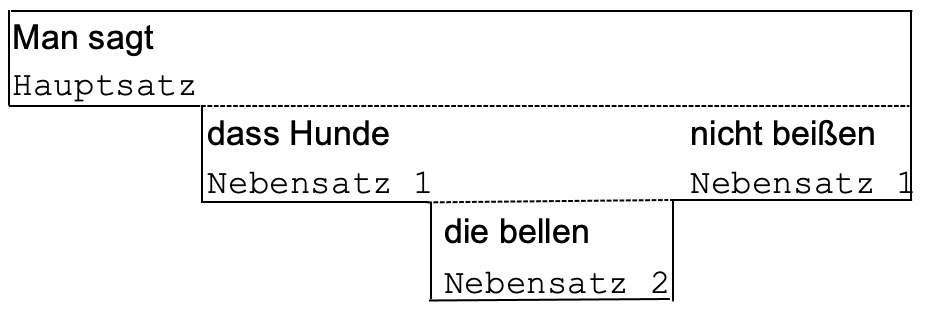
\includegraphics[width=8cm]{figures/Satzbild_Hunde.jpeg}
    %% Abbildung 

	
	\noindent\resizebox{\textwidth}{!}{
	
		\begin{tabular}{  p{3.5cm} p{3.5cm} p{3.5cm} p{3.5cm} }
			
			\hline
			\multicolumn{1}{ | l }{\makecell[l]{Man sagt \\ \small{\textcolor{gray}{Hauptsatz}}}} &&& \multicolumn{1}{ l | }{} \\   \cline{1-1} \sbdashline{2-4}
			
			& \multicolumn{1}{ | l}{\makecell[l]{dass Hunde \\ \small{\textcolor{gray}{Nebensatz 1}}}} & & 
			\multicolumn{1}{ l | }{\makecell[l]{nicht beißen \\ \small{\textcolor{gray}{}}}} \\ \cline{2-2} \sbdashline{3-4} \cline{4-4}
			
			& & \multicolumn{1}{ | l | }{\makecell[l]{die bellen \\ \small{\textcolor{gray}{ Nebensatz 2}}}} & \\ \cline{3-3} 
			
		\end{tabular}
	}
	

	



    \caption{Satzbild zu (\ref{ex:HS_NeSa_NeSa})}
    \label{Abb:Satzbild_Hunde}
\end{figure}

Die jeweilige Ebene wird auch als \textit{Grad} der Einbettung bezeichnet. Daher könnte der Nebensatz der ersten Ebene auch \textit{ersten Grades} genannt werden und der Nebensatz der zweiten Ebene entsprechend \textit{zweiten Grades}.

Nun zurück zu den Satzgliedfunktionen: Der komplexe Nebensatz \textit{dass Hunde, die bellen, nicht beißen} ist das Satzobjekt von \textit{sagt}. Es besteht die wichtigen Satzgliedtests (vgl. Kapitel \ref{chap:Konstituenz}). Der komplexe Nebensatz ist voranstellbar (\ref{ea:dassNeSaTop}), pronominalisierbar (\ref{ex:dassNeSaPrn}), auch durch ein Fragepronomen und somit auch erfragbar (\ref{ex:dassNeSaFrage}).

\ea \label{ea:NeSaSGTests}
\ea \label{ea:dassNeSaTop} [Dass Hunde, die bellen, nicht beißen,] sagt man.
\ex \label{ex:dassNeSaPrn} Man sagt [das].
\ex \label{ex:dassNeSaFrage} [Was] sagt man?
\z 
\z 

Intern besteht das Satzobjekt wieder aus Satzgliedern. Denn es enthält ein Prädikat, nämlich \textit{beißen}. Das Verb ist zweiwertig und verlangt nach einer Ergänzung im Nominativ, dem Subjekt und einer Ergänzung im Akkusativ, dem Objekt. Ein Objekt gibt es nicht. Das Verb wird einwertig gebraucht (vgl. Abschnitt~\ref{subsubsection:TestNOT}). Das Subjekt ist \textit{Hunde, die bellen}. Der Nebensatz ist Teil des Subjektes. Zum Nachweis bilden wir aus dem Nebensatz \textit{dass Hunde, die bellen, nicht beißen} einen Hauptsatz (\ref{ea:HSUmformung}). Der Nebensatz \textit{die bellen} kann nicht alleine im Vorfeld stehen (\ref{ex:RelNeSaTop}), ist nicht durch eine Pro-Form ersetzbar (\ref{ex:RelNeSaPrn}) und nicht alleine erfragbar (\ref{ex:RelNeSaFrage}). 

\ea \label{ea:NeSaAttrTests}
\ea [] {Hunde, die bellen, beißen nicht.}\label{ea:HSUmformung} 
\ex [*] {Die bellen beißen Hunde nicht.}\label{ex:RelNeSaTop}
\ex [*] {Hunde ?? beißen nicht.}\label{ex:RelNeSaPrn}
\ex [*] {Welche beißen Hunde nicht?}\label{ex:RelNeSaFrage}
\z 
\z 

Der Nebensatz \textit{die bellen} ist kein Satzglied, weil er sich auf kein Prädikat bezieht und damit von keinem Prädikat abhängt. Er bezieht sich auf \textit{Hunde}, den Kopf der Subjekt-NP und ist somit Teil des Subjekts \textit{Hunde, die bellen} und damit Attribut. Deshalb ist nur die gemeinsame Voranstellung wie in (\ref{ea:HSUmformung}) möglich.

Attribute werden in der Satzgliedanalyse nicht sichtbar, weil sie keine Satzglieder, sondern Satzgliedteile sind. Aber wenn sie über ein Prädikat wie \textit{bellen} verfügen, bestehen sie intern wieder aus Satzgliedern. Diese werden auf einer tieferen Ebene (in einer weiteren Tabellenspalte) bestimmt. Das Prädikat \textit{bellen} ist einwertig und verlangt nach einer Ergänzung im Nominativ, nach einem Subjekt. Das Subjekt ist das den Relativsatz einleitende Demonstrativpronomen \textit{die}.

Die schrittweise Analyse ausgehend vom Hauptprädikat stellen wir in der Tabelle~\ref{tab:Satzgefüge1} dar. Die im Satzbild (Abbildung~\ref{Abb:Satzbild_Hunde}) dargestellten Ebenen entsprechen bei einer Drehung um 90 Grad nach links den Spalten.

\begin{table}
  \centering
  \begin{tabular}{l|l|l|l}
    %\lsptoprule
     & Hauptsatz & 1. Nebensatzebene & 2. Nebensatzebene \\
    \hline
    \textit{Man} & Subjekt &  & \\
    \cline{2-2} 
    \textit{sagt,} & Prädikat & & \\
    \cline{2-3}
    \textit{dass} & \multirow{6}{*}{Satzobjekt} & -- & \\ \cline{3-3}
    \textit{Hunde,} &  & \multirow{3}{*}{Subjekt} & \\ \cline{4-4}
    \textit{die} & & & Subjekt \\ \cline{4-4}
    \textit{bellen,} & & & Prädikat  \\ \cline{3-4}
    \textit{nicht} & & -- & \\ \cline{3-3}
    \textit{beißen.} & & Prädikat & \\ 
    \hline 
   % \lspbottomrule
  \end{tabular}
  \caption{Satzgefüge mit zwei Einbettungsebenen}
  \label{tab:Satzgefüge1}
\end{table}

Die Nebensatzebenen müssen nicht der Reihenfolge ihres Auftretens entsprechen. Wie in (\ref{ea:HS_mehrereNeSa}) kann ein Hauptsatz auch zwei (und mehr) Nebensätze direkt in sich, also eine Ebene tiefer einbetten. 

\ea \label{ea:HS_mehrereNeSa} Jugendliche, die ihren Freunden eine Nachricht in Facebook schreiben, werden in der Regel nicht lange nachdenken, ob diese oder jene Schreibweise richtig ist.\footnote{Christa Dürscheid (2011): \textit{Zweifeln als Chance? Zweifeln als Problem? Sprachliche Zweifelsfälle im Deutschunterricht.} In: Köpcke, K.-M. \& A. Ziegler (Hrsg.): \textit{Grammatik – Lehren, Lernen, Verstehen. Zugänge zur Grammatik des Gegenwartsdeutschen.} Berlin, Boston: de Gruyter, S. 161.}
\z 

Die Einbettungsebenen stellen wir in der Abbildung~\ref{Abb:Satzbild_Jugendliche} im Satzbild\is{Satzbild} dar.

\begin{figure}
    \centering
   % 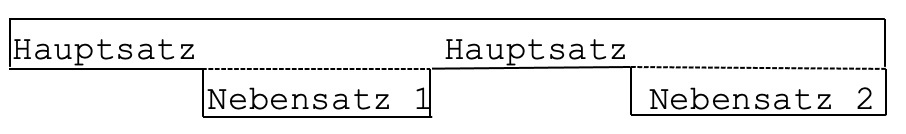
\includegraphics[width=9cm]{figures/Satzbild_Jugendliche.jpeg}
   %% Abbildung 

		\noindent\resizebox{\textwidth}{!}{
		
		\begin{tabular}{p{3cm} p{3cm} p{3cm} p{3cm} | }
			
			\hline
			\multicolumn{1}{ | l }{\makecell[l]{\small{\textcolor{gray}{Hauptsatz}}}} & & 
			\multicolumn{1}{ l }{\makecell[l]{\small{\textcolor{gray}{}}}} &  \\ 
			\cline{1-1} \sbdashline{2-2}  \cline{3-3} \sbdashline{4-4}
			
			
			&  \multicolumn{1}{ | l | }{\makecell[l]{\small{\textcolor{gray}{Nebensatz 1}}}}  & & 
		     	 \multicolumn{1}{ | l | }{\makecell[l]{\small{\textcolor{gray}{Nebensatz 2}}}}   		\\ 
		     	 \cline{2-2}  \cline{4-4}
			
		\end{tabular}
	}
	


	

	



    \caption{Satzbild zu (\ref{ea:HS_mehrereNeSa})}
    \label{Abb:Satzbild_Jugendliche}
\end{figure}

Das Prädikat des Hauptsatzes ist \textit{werden nachdenken}. Es ist zweiwertig und verlangt nach jemandem, der nachdenkt als Subjekt und nach etwas, worüber nachgedacht wird, als Präpositionalobjekt. An dessen Stelle steht der zweite Nebensatz \textit{ob diese oder jene Schreibweise richtig ist} und fungiert damit als Satzobjekt. Das Subjekt ist die komplexe NP im Vorfeld \textit{Jugendliche} zusammen mit dem ersten Nebensatz \textit{die ihren Freunden eine Nachricht in Facebook schreiben}. Beide Nebensätze sind direkt in den Hauptsatz eingebettet. Hierfür steht die gestrichelte Linie auf der Hauptsatzebene. Der erste Nebensatz ist als Attribut Bestandteil des Subjektes. Der zweite Nebensatz ist ein Satzglied, da er als Objekt direkt vom Hauptprädikat abhängt. Die interne Struktur beider Nebensätze wird in einer Spalte, direkt nach der Hauptsatzebene, analysiert, was wir in der Tabelle~\ref{tab:Satzgefüge2} zeigen. 


\begin{table}
  \centering
  \begin{tabular}{l|l|l}
    %\lsptoprule
      &  Hauptsatz & 1. Nebensatzebene \\
    \hline
    \textit{Jugendliche,} & \multirow{9}{*}{Subjekt} &  \\
    \cline{3-3} 
    \textit{die} & & Subjekt \\
    \cline{3-3}
    \textit{ihren} & & \multirow{2}{*}{Dativobjekt} \\ 
    \textit{Freunden} &  & \\ \cline{3-3}
    \textit{eine} & &  \multirow{2}{*}{Akkusativobjekt} \\ 
    \textit{Nachricht} & & \\ \cline{3-3}
    \textit{in} & & \multirow{2}{*}{Adverbial} \\ 
    \textit{Facebook} & & \\ \cline{3-3}
    \textit{schreiben,} & & Prädikat \\ \cline{2-3}
    \textit{werden} & Prädikat &  \\ \cline{2-2}
    \textit{in} & \multirow{3}{*}{Adverbial} & \\ 
    \textit{der} & & \\ 
    \textit{Regel} & & \\ \cline{2-2} 
    \textit{nicht} & \multirow{2}{*}{Adverbial} & \\ 
    \textit{lange} & & \\ \cline{2-2}
    \textit{nachdenken,} & Prädikat & \\ \cline{2-3}
    \textit{ob} & \multirow{7}{*}{Satzobjekt} & -- \\ \cline{3-3}
    \textit{diese} & & \multirow{4}{*}{Subjekt} \\
    \textit{oder} & & \\
    \textit{jene} & & \\ 
    \textit{Schreibweise} & & \\ \cline{3-3}
    \textit{richtig} & & Subjektsprädikativ \\ \cline{3-3}
    \textit{ist.} & & Prädikat \\ 
    \hline 
   %\lspbottomrule
  \end{tabular}
  \caption{Satzgefüge mit einer Einbettungsebene}
  \label{tab:Satzgefüge2}
\end{table}

\vspace{.2cm}

Bevor wir uns mit der Form und Funktion von Nebensätzen in Satzgefügen beschäftigen, fassen wir das Wichtigste zusammen. Wir haben zwischen Satzreihen und Satzgefügen unterschieden. Bei Satzreihen handelt es sich um gleichrangig miteinander verbundene Teilsätze. Im Gegensatz dazu enthält ein Satzgefüge einen nicht-gleichrangig eingebetteten Teilsatz. 


\subsection{Form und Funktion von Nebensätzen}\label{subsection:FormFktNeSa}

Nebensätze\is{Nebensatz!Funktionen} drücken wie Hauptsätze Szenarien aus. Aber sie behaupten diese nicht explizit wie letztere (vgl. Abschnitt~\ref{section:Grundlagen}). In Abschnitt~\ref{section:Satzglieder} haben wir gezeigt, dass Nebensätze die Funktion der wichtigsten Satzglieder sowie die eines Attributs übernehmen können. Sie können in einem Satz als Subjekt (\ref{ea:NeSaSG_Subjekt}), Akkusativobjekt (\ref{ex:NeSaSG_A_Objekt}), Dativobjekt (\ref{ex:NeSaSG_D_Objekt}), Direktivum (\ref{ex:NeSaSG_Dir}), Präpositionalobjekt (\ref{ex:NeSaSG_P_obj}), Prädikativ (\ref{ex:NeSaSG_Prädikativ}) und Adverbial (\ref{ex:NeSaSG_Adv}) fungieren bzw. an dessen Stelle stehen. Innerhalb eines Satzglieds können sie die Rolle des Attributs (\ref{ex:NeSaSG_Attribut}) haben.

\ea \label{ea:NeSaSGFunktion}
\ea \label{ea:NeSaSG_Subjekt} \textit{Dass eine Beteiligung an einem Einsatz im Nahen Osten in Deutschland kontrovers diskutiert wird}, hat niemanden überrascht.\footnote{Nordkurier, 27.09.2006.}
\ex \label{ex:NeSaSG_A_Objekt} Eine Kundin möchte wissen, \textit{ob dieser Pullover beim Waschen einläuft}.\footnote{Rhein-Zeitung, 24.12.2005.}
\ex \label{ex:NeSaSG_D_Objekt} Ich sah zu, \textit{wie das geschmolzene Blei aus dem Teelöffel ins kalte Wasser zischelt} [\ldots{}]\footnote{Herta Müller: \textit{Der König verneigt sich und tötet}. München: Hanser, 2003, S. 58.}
\ex \label{ex:NeSaSG_Dir} Geh, \textit{wohin dein Herz dich trägt}.\footnote{Buchtitel von Susanna Tamaro. Zürich: Diogenes, 1997.}
\ex \label{ex:NeSaSG_P_obj} Ein Passant beschwert sich, \textit{dass er keinen Platz bekommen hat}.\footnote{Mannheimer Morgen, 05.03.2002.}
\ex \label{ex:NeSaSG_Prädikativ} Die Situation ist und bleibt, \textit{wie sie ist}, man verbrennt nur seine Kraft vergeblich.\footnote{Luxemburger Tageblatt, 03.05.2018.}
\ex \label{ex:NeSaSG_Adv} \textit{Wenn es einen Anlass zum Scherzen gibt}, schmunzle ich gern einmal.\footnote{Zitat aus Loriots Film \textit{Papa ante portas}.}
\ex \label{ex:NeSaSG_Attribut} Selbst der Mann, \textit{der niemals lächelte}, hat auf seine diskrete Art Ecken und Kanten [\ldots{}]\footnote{Süddeutsche Zeitung, 25.02.2016.}
\z 
\z 

\textit{Subjunktionalsätze} werden\is{Nebensatz!Subjunktionalsatz}, wie der Name schon sagt, durch eine Subjunktion (vgl. Abschnitt~\ref{subsubsection:Subjunktion}) eingeleitet. \textit{Sub}junktionen verbinden auch Sätze, aber der Satz, den sie einleiten, ist einem anderen Satz oder einem Wort \textit{unter}geordnet. Subjunktionale Nebensätze lassen sich bezüglich ihrer syntaktischen Funktion in zwei große Gruppen einteilen: in solche mit den relativ bedeutungsleeren Subjunktionen \textit{dass} und \textit{ob} und in solche mit den bedeutungsreicheren temporalen, kausalen usw. Subjunktionen wie \textit{nachdem}, \textit{wenn}, usw. 

Die relativ\is{Nebensatz!Subjekt-/Objektfunktion} bedeutungsarmen Subjunktionen \textit{dass} und \textit{ob} leiten Nebensätze ein, die typischerweise als Subjekt- oder Objektsatz verbale Ergänzungen sind. Durch \textit{dass} wird der ausgedrückte Sachverhalt als wahr vorausgesetzt. Durch \textit{ob} bleibt das offen. Beide Subjunktionen sind in dem Nebensatz, den sie einleiten, weder Satzglied noch Attribut. Deshalb setzen wir in der Tabelle einen Strich. Die Analyse stellen wir exemplarisch für (\ref{ex:NeSaSG_A_Objekt}) in Tabelle~\ref{tab:Satzgefüge_mit_ob_Objektsatz} dar.

\begin{table}
  \centering
  \begin{tabular}{l|l|l}
    %\lsptoprule
      & Hauptsatz & 1. Nebensatzebene \\
    \hline
    \textit{Eine} & \multirow{2}{*}{Subjekt} &  \\
    \textit{Kundin} & & \\ \cline{2-2}
    \textit{möchte} & \multirow{2}{*}{Prädikat} & \\ 
    \textit{wissen,} &  & \\ \cline{2-3}
    \textit{ob} & \multirow{6}{*}{Satzobjekt} & -- \\ \cline{3-3} 
    \textit{dieser} &  & \multirow{2}{*}{Subjekt} \\ 
    \textit{Pullover} & & \\ \cline{3-3} 
    \textit{beim} &  & \multirow{2}{*}{Adverbial} \\
    \textit{Waschen} & & \\ \cline{3-3}
    \textit{einläuft.} & & Prädikat  \\ 
    \hline 
   %\lspbottomrule
  \end{tabular}
  \caption{Subjunktionaler Objekt-Nebensatz mit \textit{ob}}
  \label{tab:Satzgefüge_mit_ob_Objektsatz}
\end{table}

In den\is{Nebensatz!Attributfunktion} Abschnitten zum Bau von NPs (vgl. Abschnitt~\ref{section:NP}) und zum Bau von VPs (vgl. Abschnitt~\ref{section:VP}) sowie insbesondere zur Unterscheidung und Überführung zwischen Satzgliedern und Attributen (vgl. Abschnitt~\ref{section:SatzgliederundAttribute}) haben wir auf Nominalisierungen von Verben hingewiesen. Durch diese können auch die Subjunktionen \textit{dass} und \textit{ob} aus dem Verbal- und damit Satzgliedbereich (\ref{ex:NeSaSG_A_Objekt}) in den nominalen Bereich der Attribute vererbt werden (\ref{ea:ob_Attr}).

\ea \label{ea:ob_Attr} Ihr Wissen, \textit{ob dieser Pullover beim Waschen einläuft}, hilft ihr.
\z 

An der internen Struktur des Nebensatzes ändert das nichts, was wir in Tabelle~\ref{tab:Satzgefüge_mit_ob_Attributsatz} darstellen.

\begin{table}
  \centering
  \begin{tabular}{l|l|l}
  %  \lsptoprule
     &  Hauptsatz & 1. Nebensatzebene \\
    \hline
    \textit{Ihr} & \multirow{8}{*}{Subjekt} &  \\
    \textit{Wissen,} & & \\ \cline{3-3}
    \textit{ob} & &  -- \\ \cline{3-3} 
    \textit{dieser} &  & \multirow{2}{*}{Subjekt} \\ 
    \textit{Pullover} & & \\ \cline{3-3} 
    \textit{beim} & & \multirow{2}{*}{Adverbial} \\
    \textit{Waschen} & & \\ \cline{3-3}
    \textit{einläuft,} & & Prädikat  \\ \cline{2-3} 
    \textit{hilft} & Prädikat \\ \cline{2-2}
    \textit{ihr.} & Dativobjekt & \\
    \hline
   %\lspbottomrule
  \end{tabular}
  \caption{Subjunktionaler Attribut-Nebensatz mit \textit{ob}}
  \label{tab:Satzgefüge_mit_ob_Attributsatz}
\end{table}


Subjunktionale Nebensätze\is{Nebensatz!Adverbialfunktion} mit bedeutungsreicheren Subjunktionen wie \textit{als}, \textit{bevor}, \textit{nachdem} \textit{weil}, \textit{obwohl}, \textit{wenn}, \textit{damit}, \textit{indem} usw. leiten typischerweise Adverbialsätze ein. Sie sättigen keine Valenzstellen des Prädikats, sondern spezifizieren das ausgedrückte Szenario (vgl. Abschnitt~\ref{subsection:Adverbial}). Formal besonders sind zweiteilige Subjunktionen wie \textit{als ob}, \textit{anstatt dass}, \textit{ohne dass} oder \textit{so dass}. Bei letzterer wird heute vom Duden die Zusammenschreibung als \textit{sodass} empfohlen.

Unabhängig vom Bedeutungsumfang und von Ein- oder Zweiteiligkeit gibt es zwei wesentliche Gemeinsamkeiten: Subjunktionalsätze sind typischerweise Satzglieder eines übergeordneten Prädikats. Die Subjunktionen selber sind innerhalb des Nebensatzes, den sie einleiten, weder Satzglied noch Attribut. Deshalb setzen wir in der Tabelle auf der entsprechenden Ebene einen Strich. Das haben wir in den Tabellen~\ref{tab:Satzgefüge1}, \ref{tab:Satzgefüge2} und \ref{tab:Satzgefüge3} gesehen.

Eine formale\is{Nebensatz!verkappter} Besonderheit stellen \textit{uneingeleitete Nebensätze} (\ref{ea:verkappteNeSa}) dar. Diese bilden wir ohne Subjunktion. Folglich steht auch der finite Prädikatsteil nicht in der rechten, sondern in der linken Satzklammer. 

\ea \label{ea:verkappteNeSa}
\ea \label{ea:verkappterObjektsatz} Paul sagt, \textit{er komme später}.
\ex \label{ex:verkappterKondNeSa} \textit{Regnet es stark}, bleiben wir zu Hause.
\ex \label{ex:verkappterMODalsNeSa} Er tut so, \textit{als sehe er mich nicht}.
\z 
\z 

In (\ref{ea:verkappterObjektsatz}) könnte es heißen \textit{dass er später komme}, in (\ref{ex:verkappterKondNeSa}) \textit{wenn es stark regnet} und in (\ref{ex:verkappterMODalsNeSa}) \textit{als ob er mich nicht sehe}.    

Obwohl das finite Verb in den kursiv gesetzten Teilsätzen in (\ref{ea:verkappteNeSa}) nicht am Ende steht, handelt es sich um Nebensätze. Denn sie hängen vom Bezugsprädikat bzw. von dem anderen Teilsatz ab. Mit \citet[70]{Welke2007} nehmen wir für solche Nebensätze mit Verbzweit- und Verberststellung die Bezeichnung \textit{verkappter Nebensatz} wieder auf. 

In (\ref{ea:verkappterObjektsatz}) handelt es sich um das Objekt zu \textit{sagt}. Nach \citet[119]{Bausewein1990} stellt diese Realisierungsform die häufigere Variante dar.\footnote{Im Gegensatz zu \citet[119]{Bausewein1990} bezeichnen \citet[167]{OehlSeiler2013} solche uneingeleiteten Nebensätze als \gqq{Ausnahme}. Nach verneinten Verben des Sagens und Denkens sind solche uneingeleiteten Nebensätze weniger gebräuchlich: \textit{Er behauptete nicht,} ?\textit{er sei unschuldig}. Bei Interesse empfehlen wir auch \citet[121]{Reis1997}, die von \gqq{syntaktisch relativ unintegrierten Nebensätze[n]} schreibt.} In (\ref{ex:verkappterKondNeSa}) drückt der verkappte Nebensatz mit Verberststellung ein bedingendes Szenario aus und fungiert als konditionales Adverbial. In (\ref{ex:verkappterMODalsNeSa}) geht es um die Beschreibung der Art und Weise (\textit{als sehe er mich nicht}). Es handelt sich um ein modales Adverbial. Auf das \textit{so} gehen wir in Abschnitt~\ref{subsection:Korrelat} unter dem Stichwort \textit{Korrelat} ein.  

Nicht-subjunktionale Nebensatzeinleiter haben innerhalb des Nebensatzes, den sie einleiten, eine Satzgliedfunktion. Das ist\is{indirekter Fragesatz} der Fall bei sogenannten \textit{indirekten Frage-Nebensätzen} mit Fragewörtern wie \textit{wer}, \textit{welcher}, \textit{wo}, \textit{warum} oder durch \textit{w}-Pro-Präpositionsgruppen (vgl. Abschnitt~\ref{section:Pronominalisierung}) wie \textit{worauf}, \textit{womit}, \textit{wofür}, usw. aus. 

\ea \label{ea:Frage-NeSa}
\ea \label{ea:wissen_warum} Ich weiß doch, \textit{warum du uns das erzählst}. \footnote{Sven Regener: \textit{Herr Lehmann}. Frankfurt am Main: Eichborn, 2001, S. 137.}
\ex \label{ex:fragen_woran} Ich frage ihn, \textit{woran er leidet}.\footnote{Die Zeit, 16.03.2000}
\z 
\z 

Als Ganzes fungieren auch indirekte Frage-Nebensätze als Satzobjekt bei Verben des Fragens, (Nicht)-Wissens und Wahrnehmens. Aber innerhalb des Nebensatzes sind die Fragewörter Satzglieder. In (\ref{ea:wissen_warum}) ist \textit{warum} ein Kausaladverbial, da es für die Angabe eines Grundes für den Sachverhalt \textit{du erzählst uns das} steht. Die Pro-Form \textit{woran} steht in (\ref{ex:fragen_woran}) für das Präpositionalobjekt von \textit{leidet}. Die Analyse von (\ref{ex:fragen_woran}) stellen wir in der Tabelle~\ref{tab:FrageNeSa} dar.

\begin{table}
  \centering
  \begin{tabular}{l|l|l}
    %\lsptoprule
      & Hauptsatz & 1. Nebensatzebene \\
    \hline
    \textit{Ich} & Subjekt &  \\ \cline{2-2}
    \textit{frage} & Prädikat & \\ \cline{2-2}
    \textit{ihn,} & Akkusativobjekt & \\ \cline{2-3}
    \textit{woran} & \multirow{3}{*}{Satzobjekt} & Präpositionalobjekt \\ \cline{3-3}  
    \textit{er} & & Subjekt  \\ \cline{3-3} 
    \textit{leidet.} & & Prädikat \\ 
    \hline 
  % \lspbottomrule
  \end{tabular}
  \caption{Nebensatzeinleitende Pronomen mit Satzgliedwert}
  \label{tab:FrageNeSa}
\end{table}

Typische Attribut-Nebensätze\is{Relativsatz} sind\is{Nebensatz!Attributfunktion} \textit{Relativsätze}. Sie werden durch Pronomen wie \textit{der}, \textit{den}, \textit{dem} oder \textit{welcher}, \textit{welchem}, usw. eingeleitet (\ref{ea:DP_Rel}). 

\ea \label{ea:DP_Rel} Das ist der Mann, \textit{den}/\textit{welchen} Anna gestern getroffen hat.
\z 

Die im Relativsatz gebrauchten Pronomen kongruieren im Genus und Numerus mit dem Bezugswort. Der Kasus richtet sich nach ihrer syntaktischen Funktion im Relativsatz. Um die Formen der Pronomen geht es im Abschnitt~\ref{subsection:Pronomen_Flexion}.

Ebenso können Relativsätze durch Adverbien wie \textit{wo}, \textit{wohin} und \textit{woher} eingeleitet werden (\ref{ea:Adv_Rel}). Ihre Form ist unveränderlich.  

\ea \label{ea:Adv_Rel} Paul wohnt, \textit{wo} Fuchs und Hase sich gute Nacht sagen.
\z 

Mit Relativsätzen\is{Relativsatz!restriktiv} werden Merkmale des von einer NP Bezeichneten ausbuchstabiert. Die Merkmalsübertragung geschieht auf zwei grundlegende Arten. Durch \textit{restriktive} Relativsätze wird die Menge des potenziell Bezeichneten eingeschränkt (restringiert). So geht es in (\ref{ea:restriktivREL}) nicht um alle möglichen Menschen, sondern nur um die Untermenge der über 65-Jährigen. 

\ea \label{ea:restriktiv_appositiv}
\ea \label{ea:restriktivREL}  Der Trend betrifft jedoch hauptsächlich Menschen, \textit{die das 65. Lebensjahr überschritten haben}.\footnote{Süddeutsche Zeitung, 25.08.2015.}
\ex \label{ex:appositivREL} Die Figuren aus dem beliebten Kinderbuch, \textit{das jetzt verfilmt wurde}, gibt es beim Kaufhof.\footnote{Mannheimer Morgen, 03.12.2004.}
\z 
\z 

In (\ref{ex:appositivREL}) schränkt der\is{Relativsatz!appositiv} Relativsatz nicht die Referenz der NP ein. Er gibt eine zusätzliche Information über das von der NP Bezeichnete, weshalb man von \textit{appositiv}en Relativsätzen spricht. Diese Lesart kann durch das Hinzufügen von \textit{übrigens} getestet oder ausgelöst werden. 


In der Satzgliedanalyse wird dieser Unterschied nicht erfasst. Exemplarisch analysieren wir den Satz (\ref{ex:appositivREL}) in der Tabelle~\ref{tab:Relativsatz}.

\begin{table}
  \centering
  \begin{tabular}{l|l|l}
   % \lsptoprule
        & Hauptsatz & 1. Nebensatzebene \\
    \hline
    \textit{Die} & \multirow{9}{*}{Akkusativobjekt} &  \\ 
    \textit{Figuren} & & \\
    \textit{aus} & & \\
    \textit{dem} & & \\ 
    \textit{beliebten} & & \\ 
    \textit{Kinderbuch,} & & \\ \cline{3-3}
    \textit{das} & & Subjekt \\ \cline{3-3}
    \textit{jetzt} & & Adverbial \\ \cline{3-3}
    \textit{verfilmt} & & \multirow{2}{*}{Prädikat} \\
    \textit{wurde,} & & \\ \cline{2-3} 
    \textit{gibt} & Prädikat & \\ \cline{2-2}
    \textit{es} & Subjekt & \\ \cline{2-2}
    \textit{im} & \multirow{2}{*}{Adverbial} &  \\   
    \textit{Kaufhof.} & & \\  
    \hline 
  % \lspbottomrule
  \end{tabular}
  \caption{Relativsatz}
  \label{tab:Relativsatz}
\end{table}

Von den beschriebenen typischen Zusammenhängen zwischen Form und syntaktischer Funktion gibt es Übergänge. Diese stellen wir in dem folgenden Exkurs~\ref{Exkurs: Übergänge Nebensatzfunktionen} dar. Zuvor fassen wir das Wichtigste zusammen. 

\vspace{.2cm}

Wir haben subjunktionale von uneingeleiteten (verkappten) Nebensätzen unterschieden. 

\begin{itemize}
    \item Subjunktionale Nebensätze mit den bedeutungsarmen Subjunktionen \textit{dass} und \textit{ob} fungieren typischerweise als Subjekte oder Objekte.

    \item Subjunktionale Nebensätze mit den bedeutungsreicheren Subjunktionen wie \textit{bevor}, \textit{indem} oder \textit{weil} fungieren typischerweise als Adverbiale.

    \item Uneingeleitete Nebensätze fungieren typischerweise als Objekte zu Prädikaten des Sagens und Denkens.

\end{itemize}

Subjunktionen kommt innerhalb des Nebensatzes, den sie einleiten, kein Satzgliedstatus zu. Bei Nebensätzen, die durch Demonstrativpronomen wie \textit{der}, \textit{die}, \textit{das}, durch w-Pronomen wie \textit{wer} und \textit{was} sowie durch Frageadverbien wie \textit{wo} und \textit{wohin} eingeleitet sind, ist das nicht der Fall. Diesen Nebensatzeinleitern kommt innerhalb des Nebensatzes eine Satzgliedfunktion zu.

\begin{itemize}
    \item Indirekte Frage-Nebensätze mit \textit{wer}, \textit{was}, \textit{wo} usw. fungieren typischerweise als Objekte zu Prädikaten des Fragens, des (Nicht-)Wissens und des Wahrnehmens. Innerhalb des Nebensatzes fungiert der \textit{w}-Ausdruck als Satzglied.

    \item Relativsätze sind typischerweise Attribute zu einem Substantiv. Die Relativsatzeinleiter fungieren innerhalb des Relativsatzes als Satzglieder.
    
\end{itemize}


\begin{Exkurs}{Funktionsübergänge bei Nebensätzen}\label{Exkurs: Übergänge Nebensatzfunktionen}
    
Innerhalb bestimmter Kontexte können bestehende Nebensatzformen neue Funktionen übernehmen. Bei Nebensätzen mit \textit{dass} und \textit{ob} haben wir auf solche Funktionsübergänge schon hingewiesen. Wenn wir statt der verbalen Prädikate \textit{wissen} oder \textit{fragen} die Substantive (\textit{das}) \textit{Wissen} und (\textit{die}) \textit{Frage} gebrauchen, so werden die ursprünglichen Objektsätze zu Attributsätzen: \textit{das Wissen, dass sich die Erde erwärmt} und \textit{die Frage, ob wir das gestoppt bekommen}. 

Auch auf der Ebene der subjunktionalen Adverbialsätze kann es zu folgenden Funktionsübergängen kommen. Wir können als Adverbial angelegte konditionale \textit{wenn}-Nebensätze (\ref{ea:wenn_Adv}) dann als Satzobjekte verstehen, wenn das übergeordnete Prädikat eine entsprechende Leerstelle hat, die nicht anderweitig besetzt ist (\ref{ex:wenn_Obj}).

\ea \label{ea:wenn_Adv_Obj}
\ea [] {Anna mag Paul (dann) nicht, \textit{wenn er betrunken ist}.}\label{ea:wenn_Adv}
\ex [] {Anna mag (es) nicht, \textit{wenn Paul betrunken ist}.}\label{ex:wenn_Obj}
\ex [\#] {Anna mag es dann nicht, \textit{wenn Paul betrunken ist}.}\label{ex:wenn_Obj_*dann} 
\z 
\z 

Die originäre Funktion des Nebensatzes ist die des Adverbials (\ref{ea:wenn_Adv}). Es drückt eine Bedingung für das Paul-Nicht-Mögen-Szenario aus. Die adverbiale Funktion des Nebensatzes kann im Hauptsatz durch \textit{dann} angezeigt werden. Da \textit{mögen} zweiwertig ist, verstehen wir in (\ref{ex:wenn_Obj}) den Nebensatz als das, was nicht gemocht wird und somit als Objekt. Ohne \textit{es} (vgl. Abschnitt~\ref{subsection:Korrelat}) muss der \textit{wenn}-Satz als Objekt verstanden werden. Das Adverbial \gq{rutscht} in die vom Prädikat angelegte Objektfunktion. \citet[447]{Pittner2013} bezeichnet diese \textit{wenn}-Sätze als \gqq{Zwittererscheinung}. \citet[358]{Eisenberg2020_Satz} bezeichnet diesen \textit{wenn}-Gebrauch als den \gqq{einzige[n] Ausreißer} aus der Adverbialfunktion. Soll die Objektlesart beibehalten werden, so darf das adverbiale \textit{dann} nicht im Hauptsatz stehen (\ref{ex:wenn_Obj_*dann}). Oder aber wir verstehen \textit{es} als Pronomen, das \zB auf das Abendessen verweist. Dann verstehen wir den Nebensatz wieder als das, was er eigentlich ist, nämlich als Adverbial. Die Objektlesart in (\ref{ex:wenn_Obj}) wird durch die offene Valenzstelle des Verbs über die Adverbialfunktion gelegt. Dies führt insbesondere bei Verben \textit{sich freuen} oder \textit{sich ärgern} zu Doppeldeutigkeiten. Denn diese Verben können sowohl ein- als auch zweiwertig gebraucht werden. Nur bei zweiwertiger Lesart (\textit{sich über etw. ärgern}/\textit{freuen}) wird die adverbiale von der Objektfunktion überblendet (\ref{ea:sich_freuen_wenn}).

\ea \label{ea:sich_freuen_wenn} Anna freut sich, \textit{wenn Paul sie besucht}.
\z 

Die primäre adverbiale Lesart ist die, dass Pauls Besuch die Bedingung für Annas Freude ist. Aber durch die mögliche Zweiwertigkeit von \textit{sich} (\textit{über etw.}) \textit{freuen} kann der Nebensatz als das verstanden werden, \textit{worüber} sich Anna freut.

Auch bei Relativsätzen, die typischerweise Attribute sind, gibt es Umstrukturierungen. Manche Relativsätze bezeichnet man als \textit{freie Relativsätze}\is{Relativsatz!freier}. Von \textit{frei} wird gesprochen, weil sie kein Bezugswort im übergeordneten Satz, von dem sie abhängen, haben. Sie werden wie in (\ref{ea:uneingeleiteterREL}) durch \textit{w}-Pronomen und Adverbien eingeleitet.

\ea \label{ea:uneingeleiteterREL}
\ea \label{ea:uneingeleiteterRELwas} Früher musste man essen, \textit{was auf den Tisch kam}.
\ex \label{ex:uneingeleiteterRELwer} Er grüßt, \textit{wen er kennt}.
\ex \label{ex:uneingeleiteterRELwonach} Sie fand, \textit{wonach sie suchte}.
\ex \label{ex:uneingeleiteterRELwo} Er lebt, \textit{wo Fuchs und Hase sich gute Nacht sagen}.
\ex \label{ex:uneingeleiteterRELwohin} Er geht, \textit{wohin auch sie geht}.
\z 
\z 

Diese Relativsätze\is{Satzglied!versus Attribut} verweisen wie NPs mit einem eingebetteten attributiven Relativsatz auf Dinge, Personen oder Orte. \citet[2270--2271]{ZifHoffStr1997} bezeichnen sie deshalb als \gqq{gegenstandsfundiert}. Als Nebensätze sind sie das nicht \gq{per se}, da Sätze per Definition durch ein Prädikat und von ihm abhängige Satzglieder Szenarien ausdrücken. Sie \gq{rutschen} in eine Funktion gegenüber dem übergeordneten Prädikat. In (\ref{ea:uneingeleiteterRELwas}) geht es um Speisen, die gegessen werden, also um Objektfunktion, weshalb es sich um ein Satzobjekt handelt. Auch der Relativsatz in (\ref{ex:uneingeleiteterRELwer}) sättigt die Objektstelle von \textit{grüßt}. Das Gleiche ist in (\ref{ex:uneingeleiteterRELwonach}) der Fall. Der Relativsatz sättigt die Objektstelle von \textit{fand}. In (\ref{ex:uneingeleiteterRELwo}) wird der Relativsatz als Ort des Lebens, also in adverbialer Funktion verstanden. Der Nebensatz in (\ref{ex:uneingeleiteterRELwohin}) übernimmt die Richtungsergänzung des übergeordneten Prädikats \textit{geht} und fungiert damit als Direktivum. Die Analyse wird exemplarisch anhand von (\ref{ex:uneingeleiteterRELwonach}) in Tabelle~\ref{tab:freierRelativsatz} gezeigt.

\begin{table}
  \centering
  \begin{tabular}{l|l|l}
    %\lsptoprule
     &  Hauptsatz  & 1. Nebensatzebene \\
    \hline
    \textit{Sie} & Subjekt &  \\ \cline{2-2}
    \textit{fand,} & Prädikat & \\ \cline{2-3}
    \textit{wonach} & \multirow{3}{*}{Satzobjekt} & Präpositionalobjekt \\ \cline{3-3}
    \textit{sie} &  & Subjekt  \\ \cline{3-3}   
    \textit{suchte.} & & Prädikat \\ 
    \hline 
  % \lspbottomrule
  \end{tabular}
  \caption{Freier Relativsatz}
  \label{tab:freierRelativsatz}
\end{table}

Dass diese Relativsätze \gq{eigentlich} Attribute auf nominaler und nicht Satzglieder auf verbaler Ebene sind, zeigt die mögliche Umformung. Durch ein Pronomen im Hauptsatz werden sie wieder bei gleicher Bedeutung zu Attributen (\ref{ea:uneingeleiteterRELKOR}).

\ea \label{ea:uneingeleiteterRELKOR}
\ea \label{ea:uneingeleiteterRELwasKOR} Früher musste man \textit{das} essen, \textit{was auf den Tisch kam}.
\ex \label{ex:uneingeleiteterRELwerKOR} Er grüßt \textit{den}, \textit{den er kennt}.
\ex \label{ex:uneingeleiteterRELwonachKOR} Sie fand \textit{das}, \textit{wonach sie suchte}.
\ex \label{ex:uneingeleiteterRELwoKOR} Er lebt \textit{dort}, \textit{wo Fuchs und Hase sich gute Nacht sagen}.
\ex \label{ex:uneingeleiteterRELwohinKOR} Er geht \textit{dorthin}, \textit{wohin auch sie geht}.
\z 
\z 

Die Analyse zeigen wir exemplarisch anhand von (\ref{ex:uneingeleiteterRELwonachKOR}) in Tabelle~\ref{tab:Relativsatz_mit_pronominalem_Bezugswort}. Der Relativsatz erfüllt jetzt seine eigentliche Funktion als Attribut innerhalb des Akkusativobjekts \textit{das, wonach sie suchte}. Seine interne Struktur bleibt wie in \ref{tab:freierRelativsatz} unverändert.

\begin{table}
  \centering
  \begin{tabular}{l|l|l}
    %\lsptoprule
     & Hauptsatz &  1. Nebensatzebene \\
    \hline
    \textit{Sie} & Subjekt &  \\ \cline{2-2}
    \textit{fand} & Prädikat & \\ \cline{2-2}
    \textit{das,} & \multirow{4}{*}{Akkusativobjekt} & \\ \cline{3-3}
    \textit{wonach} & & Präpositionalobjekt \\ \cline{3-3}
    \textit{sie} &  & Subjekt  \\ \cline{3-3}   
    \textit{suchte.} & & Prädikat \\  
    \hline
 %  \lspbottomrule
  \end{tabular}
  \caption{Relativsatz mit pronominalem Bezugswort}
  \label{tab:Relativsatz_mit_pronominalem_Bezugswort}
\end{table}

Der \gq{Ausflug} freier Relativsätze in die Domäne der Satzglieder wird formal nur beim Vergleich von (\ref{ex:uneingeleiteterRELwer}) \textit{grüßt, wen er kennt} mit (\ref{ex:uneingeleiteterRELwerKOR}) \textit{grüßt den, den er kennt} ersichtlich. 

Andere Indizien dafür, dass es sich bei Satzgliedern in Form von Relativsätzen um eine grammatische Nische handelt, bietet der Vergleich von valenziell angelegten indirekten Frage-Nebensätzen mit freien Relativsätzen. \citet[346]{Eisenberg2020_Satz} und \citet[446--446]{Pittner2013} weisen auf eine Doppeldeutigkeit hin, die durch Prädikate wie \textit{verrät} in (\ref{ea:verratenFragesatz_frRel}) möglich ist. Wir können \textit{verraten} als ein Mitteilungsverb verstehen, mit dem zu verratenden Ereignis als Objektsatz (\textit{verraten}, \textit{dass}) oder im Sinne von \gq{denunzieren} (\textit{jemanden verraten)}, das nach einem Akkusativobjekt verlangt.

\ea \label{ea:verratenFragesatz_frRel} Sie verrät nicht, \textit{wen sie liebt}.\footnote{Das Beispiel stammt aus \citet[447]{Pittner2013}.}
\z 

Entweder geht es um einen indirekten Frage-Nebensatz. Dann bezieht sich das Szenario \textit{wen sie liebt} als Satzobjekt auf das Prädikat \textit{verrät}. Eine Paraphrase wäre: \gq{sie sagt nicht, wen sie liebt}. In diesem Fall kann kein Pronomen als Bezugswort hinzugefügt werden, weil es kein freier Relativsatz ist (\ref{ea:Frage_ohne_Bezug}). Oder aber wir interpretieren den Nebensatz als freien Relativsatz, also wie eine Entität. Die Paraphrase wäre: \gq{Sie verrät nicht die geliebte Person}. In diesem Fall kann ein Pronomen als Bezugswort eingefügt werden und aus dem freien Relativsatz wird wieder ein Attributsatz wie in (\ref{ex:frRel_mit_Bezug}). 

\ea \label{ea:TestFrage_Relativ}
\ea [*] {Sie verrät (\gq{sagt}) nicht den, den sie liebt.}\label{ea:Frage_ohne_Bezug} 
\ex [] {Sie verrät nicht den, den sie liebt.}\label{ex:frRel_mit_Bezug}
\z 
\z 

Dass Relativsätze\is{Nebensatz!weiterführender} in anderer als der Attributfunktion Nischen sind, zeigt sich auch an sogenannten \textit{weiterführenden Nebensätzen}. Diese sehen aus wie freie Relativsätze mit \textit{w}-Wörtern. Aber sie können nicht wie eine NP als Satzglied auf das übergeordnete Prädikat bezogen werden, weil dieses wie \textit{schneien} in (\ref{ea:regnen_worüber}) gar nicht über eine entsprechende Leerstelle verfügt.

\ea \label{ea:regnen_worüber} Es schneite endlich, worüber sich die Kinder freuten.
\z 

In diesem Fall ist der Relativsatz funktional nicht in den übergeordneten Satz eingebettet. Er bezieht sich auf das gesamte Schneien-Szenario, in dem er keinen Satzgliedwert hat. Die Analyse zeigen wir in Tabelle~\ref{tab:weiterführenderNeSa}.

\begin{table}
  \centering
  \begin{tabular}{l|l|l}
    %\lsptoprule
     &  Hauptsatz  &  1. Nebensatzebene \\
    \hline
    \textit{Es} & Subjekt &  \\ \cline{2-2}
    \textit{schneite} & Prädikat & \\ \cline{2-2}
    \textit{endlich,} & Kommentaradverbial \\ \cline{2-3}
    \textit{worüber} & & Präpositionalobjekt \\ \cline{3-3}
    \textit{sich} &  & Prädikat  \\ \cline{3-3}   
    \textit{die} & & \multirow{2}{*}{Subjekt} \\ 
    \textit{Kinder} & & \\ \cline{3-3} 
    \textit{freuten.} & & Prädikat \\
  % \lspbottomrule
  \hline 
  \end{tabular}
  \caption{Weiterführender Nebensatz}
  \label{tab:weiterführenderNeSa}
\end{table}

Wirklich \textit{frei} sind Relativsätze, wie andere Nebensätze, nie. Denn sie sind strukturell als Attribute eines Bezugsworts angelegt. Gibt es dieses Bezugswort nicht, bleiben zwei Möglichkeiten. Entweder passt der Relativsatz wie eine NP, deren Teil er gewöhnlich ist, in die Leerstelle eines Prädikats als Satzglied (sogenannter \textit{freier Relativsatz}). Dann ist er nicht frei, sondern in Satzgliedfunktion gebunden. Oder er fungiert als sogenannter \textit{weiterführender} Nebensatz zu dem vom übergeordneten Prädikat und dessen Satzgliedern ausgedrückten Szenario. In diesem Fall bezieht er sich analog zum Nomen auf ein ganzes Szenario, als wäre es ein Gegenstand. Dafür spricht die Doppeldeutigkeit in (\ref{ea:lesen_was}). 

\ea \label{ea:lesen_was} Er liest, \textit{was ihn interessiert}.
\z 

Entweder wird \textit{was ihn interessiert} gegenstandsfundiert als Objekt des zweiwertigen Prädikats \textit{liest} verstanden im Sinne von \gq{er liest das, was ihn interessiert}. Oder der Nebensatz bezieht sich auf das einwertige Lesen-Szenario im Sinne von: \gq{Er liest. Das interessiert ihn}. In diesem Fall hat der Nebensatz im übergeordneten Satz keine Funktion.

Beide Lesarten stellen wir nur bezüglich des Satzganzen in Tabelle~\ref{tab:weiterführenderNeSa_frRel} dar. Die interne Struktur des Nebensatzes bleibt unverändert: \textit{was} ist Subjekt, \textit{ihn} Akkusativobjekt und \textit{interessiert} Prädikat.

\begin{table}
  \centering
  \begin{tabular}{l|l|l}
   % \lsptoprule
      & Prädikatsbezug  & Satzbezug\\
    \hline
    \textit{Er} & \multicolumn{2}{c}{Subjekt}\\ \cline{2-3}
    \textit{liest,} & \multicolumn{2}{c}{Prädikat} \\ \cline{2-3}
    \textit{was} & \multirow{3}{*}{Satzobjekt} & \\ 
    \textit{ihn} & & \\ 
    \textit{interessiert.} &  & \\ 
    \hline 
  % \lspbottomrule
  \end{tabular}
  \caption{Freier Relativsatz oder weiterführender Nebensatz}
  \label{tab:weiterführenderNeSa_frRel}
\end{table}

\end{Exkurs}



\subsection{Korrelat oder Kern-Attribut-Beziehung}\label{subsection:Korrelat}

Als \textit{Korrelate} bezeichnet\is{Korrelat} man Wörter in einem übergeordneten Satz, die sich auf einen abhängigen Nebensatz beziehen. Sie korrelieren mit diesem. Der Prototyp ist\is{es@\textit{es}!Korrelat} \textit{es} im Mittelfeld des übergeordneten Satzes. Dieses \textit{es} verweist auf einen im Nachfeld stehenden Nebensatz in Objekt- (\ref{ea:es_Objekt}) oder Subjektfunktion (\ref{ex:es_Subjekt}). In beiden Sätzen könnte \textit{es} auch weggelassen werden, was durch Klammern dargestellt wird. Bei wenigen Verben ist es obligatorisch.\footnote{\citet[99]{HelbigBuscha} geben eine Übersicht über Verben mit obligatorischem, fakultativem und unmöglichem Korrelat.}

\ea \label{ea:es_Korrelat}
\ea \label{ea:es_Objekt} Sie bedauert (\textit{es}), \textit{dass die Nachtzüge verschwinden}.\footnote{Süddeutsche Zeitung, 10.12.2016.}
\ex \label{ex:es_Subjekt} Wen interessiert (\textit{es}), \textit{dass immer mehr Menschen an den Folgen von Industrie- und Verkehrsverschmutzungen sterben}?\footnote{Rhein-Zeitung, 22.03.2018.} 
\z 
\z 


\begin{Definition}{Korrelat}

\noindent 
Korrelate verweisen innerhalb eines Satzes aus einem übergeordneten Teilsatz auf einen vorangehenden oder folgenden untergeordneten Teilsatz. 
\end{Definition}



Anstelle der Satzgefüge mit oder ohne Korrelat in (\ref{ea:es_Korrelat}) sind auch zwei Hauptsätze denkbar (\ref{ea:HS_HS_es_Prn}). Das Pronomen \textit{es} sättigt dann im jeweils zweiten Satz die vom Verb geforderte Objekt- (\ref{ea:es_Objekt_Prn}) bzw. die Subjektstelle (\ref{ex:es_Subjekt_Prn}) und verweist auf die im jeweils ersten Hauptsatz ausgedrückte Situation.

\ea \label{ea:HS_HS_es_Prn}
\ea \label{ea:es_Objekt_Prn} Die Nachtzüge verschwinden. Sie bedauert es.
\ex \label{ex:es_Subjekt_Prn} Immer mehr Menschen sterben an den Folgen von Industrie- und Verkehrsverschmutzungen. Wen interessiert es? 
\z 
\z 

Möglich wäre es auch, den jeweils ersten Hauptsatz als Nebensatz direkt, das heißt ohne Korrelat, in den zweiten Hauptsatz zu integrieren. In diesem Fall handelt es sich um ein Satzobjekt bzw. ein Subjekt. Die Nebensätze sind dann voranstellbar (\ref{ea:es_Korrelat_NeSa_Top}).

\ea \label{ea:es_Korrelat_NeSa_Top}
\ea \label{ea:es_Objekt_NeSa_Top} \textit{Dass die Nachtzüge verschwinden}, bedauert sie. 
\ex \label{ex:es_Subjekt_NeSa_Top} \textit{Dass immer mehr Menschen an den Folgen von Industrie- und Verkehrsverschmutzungen sterben}, interessiert wen? 
\z 
\z 

Bei dem Ausdrucksmuster mit Korrelat und Nebensatz (\ref{ea:es_Korrelat}) stellt sich die Frage nach ihrem jeweiligen syntaktischen Status. Denn eine Objekt- oder Subjektstelle kann nur einmal besetzt werden (vgl. Abschnitt~\ref{subsubsection:TestINSP}). 

Im Rahmen der Satzgliedtheorie bietet sich primär die folgende Analyse an: Das Pronomen \textit{es} ist in (\ref{ea:es_Objekt}) der Kern des Akkusativobjekts und in (\ref{ex:es_Subjekt}) der Kern des Subjekts. Die Nebensätze sind dann Attribute innerhalb des Akkusativobjekts bzw. innerhalb des Subjekts. Strukturen dieser Art haben wir bereits bei den sogenannten freien Relativsätzen kennengelernt, wenn sie an ein Pronomen im übergeordneten Satz gebunden werden (\textit{das finden, wonach gesucht wird}).


Attributsätze können eigentlich nur zusammen mit ihrem pronominalen Bezugswort vorangestellt werden (\ref{ea:Prn_Attr_Top}). Aber \textit{es} kann gerade das nicht (\ref{ex:*es_Attr_Top}).

\ea \label{ea:NeSa_Kor_Top}
\ea [] {\textit{Ihn, der alles verloren hat,} bedauert sie.}\label{ea:Prn_Attr_Top}
\ex [*] {\textit{Es, dass die Nachtzüge verschwinden,} bedauert sie.}\label{ex:*es_Attr_Top}
\z 
\z 


Die Stellungseigenschaften und die Tatsache, dass gerade der Nebensatz die inhaltliche Füllung des Satzglieds gewährleistet, sprechen gegen die Bestimmung von \textit{es} als Kern des Subjekts oder Objekts mit integriertem Attributsatz. Das Korrelat\is{es@\textit{es}!Korrelat} \textit{es} zeigt nicht auf eine Entität oder auf ein Geschehen, welche durch den Nebensatz eingegrenzt oder näher bestimmt würde. \textit{Es} ist nicht betonbar und nicht fokussierbar (*\textit{ihn interessiert nur es, dass}). 

Das Korrelat \textit{es} kündigt im Mittelfeld an, dass später noch ein Objekt oder Subjekt in Form eines Nebensatzes folgt.\footnote{\citet[907]{Oppenrieder2006} schreibt valenzgebundenen satzförmigen Ausdrücken eine \gqq{potentielle Ankündbarkeit} durch ein Korrelat zu. In diesem Sinne bezeichnet \citet[589]{Agel2017} die Funktion von \textit{es} als \gqq{kategoriale Anzeige}.} Dabei leistet das Pronomen, was der Nebensatz nicht kann. Es erfüllt als Nominativ- oder Akkusativpronomen die formale Valenzforderung des Verbs, welche inhaltlich später durch den Nebensatz gefüllt wird. In diesem Sinne beschreibt \citet[167]{Breindl1989} die Funktion als \gqq{vorausweisende Dekodierungshilfe}.\footnote{Für weitere textuelle Faktoren verweisen wir auf \citet[453--454]{Pittner2013}.} 

\citet[353]{Eisenberg2020_Satz} bestimmt das Korrelat als formalen, da kasustragenden Kopf und den Nebensatz als semantischen Kern derjenigen Konstituente, die als Objekt oder Subjekt fungiert.\footnote{Letztlich geht es um eine analoge Analyse zum Artikel als grammatischem und dem Nomen als semantischem Zentrum einer NP. Eine knappe Übersicht und Kritik bietet \citet[451]{Pittner2013}.} Wir stellen die Analyse in der Tabelle~\ref{tab:ObjKorr_NeSaObj} anhand von (\ref{ea:es_Objekt}) dar. 

\begin{table}
  \centering
  \begin{tabular}{l|l|l}
    %\lsptoprule
      &  Hauptsatz   &  1. Nebensatzebene \\
    \hline
    \textit{Sie} & Subjekt  & \\ \cline{2-2}
    \textit{bedauert} & Prädikat  & \\ \cline{2-2} 
    \textit{es,} & Akk-Obj-Korrelat & \\ \cline{2-3} 
    \textit{dass} & \multirow{4}{*}{Satzobjekt} & -- \\ \cline{3-3}
    \textit{die} & & \multirow{2}{*}{Subjekt} \\ 
    \textit{Nachtzüge} & & \\ \cline{3-3}
    \textit{verschwinden.} & & Prädikat \\
    \hline 
  % \lspbottomrule
  \end{tabular}
  \caption{Objekt-Korrelat und Satzobjekt}
  \label{tab:ObjKorr_NeSaObj}
\end{table}

Analog werden mit \citet[157--158]{Breindl1989} nicht betonte korrelierende Formen wie \textit{drauf} in (\ref{ea:drauf_warten_dass}) als\is{Korrelat} Präpositionalobjekt-Korrelat analysiert.

\ea \label{ea:drauf_warten_dass} Ich habe lange \textit{drauf} gewartet, \textit{dass das endlich jemand ausspricht}.\footnote{profil, 13.03.2000.}
\z 

Die Nicht-Betonung wird besonders dann ersichtlich, wenn der zeigende pronominale Teil um den Vokal \textit{a} reduziert ist wie \textit{drauf} statt \textit{darauf} in (\ref{ea:drauf_warten_dass}). Bleibt der Vokal, so liegt die Betonung auf der Präposition, nicht auf dem verweisenden Teil, also \textit{darAUF}. Auch hier handelt es sich um ein Korrelat und nicht um das Bezugswort eines Attributsatzes. Beide zusammen können nicht vorangestellt werden (\ref{ea:*drauf_Top}).

\ea \label{ea:*drauf_Top} *\textit{Drauf, dass das endlich jemand ausspricht,} habe ich lange gewartet.
\z 

Das\is{Korrelat} Korrelat \textit{drauf} erfüllt rein formal die vom Verb geforderte Präposition, was der Nebensatz nicht kann. Wenn ein Verb verschiedene Grundvalenzen hat wie \textit{gegen etw. kämpfen} im Gegensatz zu \textit{für etw. kämpfen}, dann schafft erst das Korrelat klare Verhältnisse: \textit{daFÜR kämpfen, dass} vs. \textit{daGEGen kämpfen, dass}.\footnote{Cf. \citet[186--187]{Bausewein1990}.}    

Anders sieht\is{Nebensatz!Attributfunktion} es aus, wenn der zeigende Teil \textit{da-} betont wird. Heißt es \textit{DArauf}, dann lässt sich die Gesamtstruktur am besten mit einem Bezugswort und einem attributiven Nebensatz vergleichen. Dafür, dass beide zusammen ein Satzglied sind, spricht, dass sie zusammen vorangestellt werden können wie in (\ref{ea:DArauf_dass_Satzobjekt}).

\ea \label{ea:DArauf_dass_Satzobjekt} \textit{Darauf, dass er diesen Moment einfangen konnte}, hatte Paul Nicklen wochenlang gewartet.\footnote{Süddeutsche Zeitung, 19.10.2012.}
\z 

Der Nebensatz kann hier als Attribut und damit Teil der Pro-Form \textit{darauf} analysiert werden. Folglich gibt es auch keinen Objektsatz, sondern ein Präpositionalobjekt, zu dem ein Nebensatzattribut gehört. Die Analyse wird in der Tabelle~\ref{tab:ProPräp_NeSa_Atrribut} gezeigt. 

\begin{table}
  \centering
  \begin{tabular}{l|l|l}
    %\lsptoprule
      &  Hauptsatz   &  1. Nebensatzebene \\
    \hline
    \textit{Darauf,} & \multirow{7}{*}{Präpositionalobjekt} & \\ \cline{3-3}
    \textit{dass} &  & -- \\ \cline{3-3}
    \textit{er} & & Subjekt  \\ \cline{3-3} 
    \textit{diesen} & & \multirow{2}{*}{Akkusativobjekt} \\  
    \textit{Moment} & & \\ \cline{3-3}
    \textit{einfangen} & & \multirow{2}{*}{Prädikat} \\ 
    \textit{konnte,} & & \\ \cline{2-3}
    \textit{hatte} & Prädikat & \\ \cline{2-2}
    \textit{Paul} & \multirow{2}{*}{Subjekt} \\ 
    \textit{Nicklen} & & \\ \cline{2-2}
    \textit{wochenlang} & Adverbial & \\ \cline{2-2}
    \textit{gewartet.} & Prädikat & \\ 
    \hline 
  % \lspbottomrule
  \end{tabular}
  \caption{Kern und Nebensatzattribut als Präpositionalobjekt}
  \label{tab:ProPräp_NeSa_Atrribut}
\end{table}

Auch in diesen Konstruktionen zeigt das pronominale Element genauso wie das Korrelat kategorial an, dass es sich um ein Präpositionalobjekt handelt. Aber es fokussiert via Betonung zusätzlich den Nebensatz und macht ihn somit gegenüber dem kategorialen Korrelat in der Informationsstruktur prominenter. \citet[592]{Agel2017} bezeichnet die betonten Formen daher auch als \gqq{Fokuskorrelat} und die unbetonten kategorialen Korrelate als \gqq{Hintergrundkorrelat}. Damit geht einher, dass die Fokussierung des Nebensatzes durch Voranstellung nur mit den betonten Pronomen, aber niemals mit den unbetonten möglich ist. 

Die\is{es@\textit{es}!Korrelat} Verbindung zwischen dem Korrelat \textit{es} im Mittelfeld und dem im Nachfeld folgenden Nebensatz lässt sich mit keiner der bekannten Strukturen befriedigend beschreiben. Diesem Sonderstatus entspricht die Bezeichnung als Objekt- oder Subjekt-Korrelat zu einem Satzobjekt oder Subjekt. Bei betonten Pro-Formen und folgendem Nebensatz lässt sich immer noch ein Bezug zu der bekannten Beziehung zwischen Bezugswort und Attribut als ein Satzglied herstellen. 

Analog\is{Korrelat} analysieren wir andere Fälle mit betonbaren Bezugswörtern. Dies gilt, wie \citet[437]{Wegener2013} zeigt, meistens bei dem Dativpronomen \textit{dem} wie in (\ref{ea:DATdem,dass}) sowie bei dem zu \textit{es} betonbaren Pendant \textit{das} wie in (\ref{ex:AKKdas,dass}).

\ea \label{ea:anderePRN_NeSa}
\ea \label{ea:DATdem,dass} Das ist verfassungswidrig und widerspricht \textit{dem}, \textit{dass alle gleich sein sollen}.\footnote{Nordkurier, 20.05.2009.}
\ex \label{ex:AKKdas,dass} Ich denke, die Fans haben \textit{das} gesehen, \textit{dass sie auf mich zählen können}.\footnote{Hannoversche Allgemeine, 18.05.2017.}
\z 
\z 

Auch hier sind Bezugswort und Nebensatz zusammen voranstellbar (\ref{ea:anderePRN_NeSaTOP}), was dafür spricht, sie als \textit{ein} Satzglied zu analysieren.

\ea \label{ea:anderePRN_NeSaTOP}
\ea \label{ea:DATdem,dassTOP} \textit{Dem, dass alle gleich sein sollen,} widerspricht das und ist verfassungswidrig. 
\ex \label{ex:AKKdas,dassTOP} \textit{Das, dass sie auf mich zählen können}, haben die Fans gesehen, denke ich. 
\z 
\z 

Exemplarisch zeigen wir die Analyse für (\ref{ex:AKKdas,dass}) in der Tabelle~\ref{tab:ProDAS_NeSa_Atrribut}. Hierzu sei an den Begriff \textit{verkappter Nebensatz} erinnert. Trotz Verbzweitstellung hängt der Satz \textit{die Fans haben das gesehen} vom übergeordneten Prädikat \textit{denke} ab. Somit handelt es sich um ein als verkappter Nebensatz ausgedrücktes Satzobjekt. Das Akkusativobjekt \textit{das, dass die Fans auf mich zählen können} ist diskontinuierlich. Denn \textit{das} steht im Mittelfeld, \textit{gesehen} bildet die rechte Satzklammer und der Attributsatz \textit{dass die Fans auf mich zählen können} steht im Nachfeld. 

\begin{table}
  \centering
  \begin{tabular}{l|l|l|l}
   % \lsptoprule
      & Hauptsatz  & 1. Nebensatzebene &  2. Nebensatzebene \\
    \hline
    \textit{Ich} & Subjekt & & \\ \cline{2-2}
    \textit{denke,} & Prädikat  & & \\ \cline{2-3}
    \textit{die} & \multirow{12}{*}{Satzobjekt} & \multirow{2}{*}{Subjekt} &  \\  
    \textit{Fans} & & & \\ \cline{3-3}  
    \textit{haben} & & Prädikat & \\ \cline{3-3}
    \textit{das} & & Akkusativobjekt & \\ \cline{3-3} 
    \textit{gesehen,} & & Prädikat \\ \cline{3-4}
    \textit{dass} & & \multirow{6}{*}{Akkusativobjekt} & -- \\ \cline{4-4}
    \textit{sie} & & & Subjekt \\ \cline{4-4} 
    \textit{auf} & & & \multirow{2}{*}{Präpositionalobjekt} \\ 
    \textit{mich} &  & & \\ \cline{4-4}
    \textit{zählen} & & & \multirow{2}{*}{Prädikat} \\
    \textit{können.} & & & \\
    \hline 
  % \lspbottomrule
  \end{tabular}
  \caption{Kern und Nebensatzattribut als Akkusativobjekt}
  \label{tab:ProDAS_NeSa_Atrribut}
\end{table}

Die Kern-Attribut-Analyse übernehmen wir auch für adverbiale Nebensätze mit \textit{weil} und \textit{wenn}, die ein fakultatives (da valenzunabhängiges) betonbares Bezugswort, nämlich \textit{deshalb} und \textit{dann}, im übergeordneten Satz haben (\ref{ea:Bezugswort_AdvNeSa}).

\ea \label{ea:Bezugswort_AdvNeSa}
\ea \label{ea:deshalb_weil} Wir haben diesen Schritt \textit{deshalb} gemacht, \textit{weil es ein massiver Wunsch junger Eltern war}.\footnote{Niederösterreichische Nachrichten, 22.12.2010.}
\ex \label{ex:dann_wenn} Ein Versteck ist nur \textit{dann} gut, \textit{wenn es niemand kennt}.\footnote{Rhein-Zeitung, 12.09.2015.}
\z 
\z 

Auch hier gilt, dass das Bezugswort und der Nebensatz gemeinsam voranstellbar sind (\ref{ea:Bezugswort_AdvNeSaTOP}), was für ihren Status als \textit{ein} Satzglied (Kern und Attribut) spricht.

\ea \label{ea:Bezugswort_AdvNeSaTOP}
\ea \label{ea:deshalb_weilTop} \textit{Deshalb, weil es ein massiver Wunsch junger Eltern war,} haben wir diesen Schritt gemacht. 
\ex \label{ex:dann_wennTOP} \textit{Dann, wenn es niemand kennt}, ist ein Versteck gut.  
\z 
\z 

Exemplarisch zeigen wir in der Tabelle~\ref{tab:deshalb_weil} die Analyse für (\ref{ea:deshalb_weil}).

\begin{table}
  \centering
  \begin{tabular}{l|l|l}
   % \lsptoprule
      &  Hauptsatz   &  1. Nebensatzebene \\
    \hline
    \textit{Wir} & Subjekt & \\ \cline{2-2}
    \textit{haben} & Prädikat  & \\ \cline{2-2}
    \textit{diesen} & \multirow{2}{*}{Akkusativobjekt} & \\  
    \textit{Schritt} & &  \\ \cline{2-2}  
    \textit{deshalb} & Adverbial & \\ \cline{2-2}
    \textit{gemacht,} & Prädikat & \\ \cline{2-3} 
    \textit{weil} & \multirow{8}{*}{Adverbial} & -- \\ \cline{3-3}
    \textit{es} & & Subjekt  \\ \cline{3-3}
    \textit{ein} & & \multirow{5}{*}{Subjektsprädikativ} \\ 
    \textit{massiver} & & \\ 
    \textit{Wunsch} &  & \\ 
    \textit{junger} & & \\
    \textit{Eltern} & & \\ \cline{3-3}
    \textit{war.} & & Prädikat\\ 
    \hline 
 %  \lspbottomrule
  \end{tabular}
  \caption{Kern und Nebensatzattribut als Adverbial}
  \label{tab:deshalb_weil}
\end{table}

Ist das Bezugswort betont, so kommt noch eine weitere Möglichkeit der Fokussierung durch sogenannte Linksversetzung des Nebensatzes ins Vorvorfeld (vgl. Abschnitt~\ref{subsection:Vorfeld}) hinzu. Das betonte Pronomen greift den Nebensatz direkt wieder auf und integriert ihn syntaktisch. Dies wird in (\ref{ea:LinksheraussetzungNeSa_Korr}) gezeigt.

\ea \label{ea:LinksheraussetzungNeSa_Korr}
\ea \label{ea:dass_darauf_VF} \textit{Dass er diesen Moment einfangen konnte}, \textit{darauf} hatte Paul Nicklen wochenlang gewartet.
\ex \label{ex:dass_das_VF} \textit{Dass sie auf mich zählen können}, \textit{das} haben die Fans gesehen, denke ich.
\ex \label{ex:weil_deshalb_VF} \textit{Weil es ein massiver Wunsch junger Eltern war}, \textit{deshalb} haben wir das gemacht.
\ex \label{ex:wenn_dann_VF} \textit{Wenn es niemand kennt}, \textit{dann} ist ein Versteck gut.
\z
\z 

Bei dieser Stellung wird das enge attributive Verhältnis aufgelöst. Den Nebensatz analysieren wir als \gqq{lose, assoziierte Beigabe mit freiem Satzgliedstatus}, wie wir eingangs \citet[1488]{ZifHoffStr1997} zitiert haben. Die Satzgliedfunktion Präpositionalobjekt übernimmt jetzt in (\ref{ea:dass_darauf_VF}) einzig die Pro-Form \textit{darauf} mit betontem \textit{da}. 


\subsection{Infinitiv- und Partizipial-Konstruktionen}\label{subsection:NebensatzähnlicheK}

Manche Infinitiv- und Partizipial-Konstruktionen werden wie Nebensätze gebraucht. Wie diese können sie gegenüber einem übergeordneten Prädikat Satzgliedfunktionen übernehmen. Anders als diese verfügen sie jedoch nur über ein infinites Prädikat (vgl. Abschnitt~\ref{section:VP}), weshalb man auch von nebensatzähnlichen Konstruktionen spricht. Das Prädikat wird durch einen Infinitiv wie in (\ref{ea:NeSa_Inf}) oder durch ein Partizip wie in (\ref{ex:NeSa_Part}) gebildet. Daraus folgt, dass sie syntaktisch keine Leerstelle eröffnen, die durch ein Subjekt gefüllt werden kann. Auf dieses muss durch den Kontext geschlossen werden (vgl. Abschnitt~\ref{section:VP} unter dem Stichwort \textit{infinite Verbalphrase}). Deshalb spricht man auch von \textit{satzwertigen Konstruktionen}. 

\ea \label{ea:nebensatzähnlich}
\ea \label{ea:NeSa_Inf} Die Eisenbahner haben gestern versucht, die Reifen sämtlicher Busse \textit{zu zerschießen}.\footnote{Jenny Erpenbeck: \textit{Wörterbuch}. Frankfurt am Main: Eichborn, 2004, S. 55.}
\ex \label{ex:NeSa_Part} Gerade im Dorf \textit{angekommen}, wohnen sie dem Begräbnis ihres Großvaters bei.\footnote{Süddeutsche Zeitung, 07.01.2004.}
\z 
\z 

Infinitivformen wie \textit{zu zerschießen} in (\ref{ea:NeSa_Inf}) können\is{Infinitivkonstruktion}   \textit{Infinitivkonstruktionen} bilden. Von dem infiniten Prädikat können bis auf das Subjekt andere Satzglieder wie \textit{die Reifen sämtlicher Busse} als Akkusativobjekt abhängen. Als ganze Konstruktion steht \textit{die Reifen sämtlicher Busse zu zerschießen} in Objektfunktion zum übergeordneten Prädikat \textit{versucht}. Es kann somit auch als Satzobjekt bezeichnet werden. Die Infinitiv-Konstruktion verhält sich wie andere Satzglieder. Sie ist voranstellbar (\ref{ea:Inf_Top}) und pronominalisierbar (\ref{ex:Inf_Prn}), also auch durch ein Fragepronomen erfragbar (\ref{ex:Inf_Frage}). Bestandteil des infiniten Prädikats ist \textit{zu}. 

\ea \label{ea:Inf_SG_Tests}
\ea \label{ea:Inf_Top} [Die Reifen sämtlicher Busse zu zerschießen], haben die Eisenbahner gestern versucht. 
\ex \label{ex:Inf_Prn} Die Eisenbahner haben [das] gestern versucht.
\ex \label{ex:Inf_Frage} [Was] haben die Eisenbahner gestern versucht?
\z 
\z 

Infinitiv-Konstruktionen können die gleichen\is{Infinitivkonstruktion!mit Satzgliedfunktion}  Satzgliedfunktionen wie andere Nebensätze (mit und ohne Korrelat) erfüllen. Das hängt vom übergeordneten Prädikat ab. Die Erweiterung des infiniten Prädikats ist abhängig von dessen Valenz. So kann auch ein \textit{zu}-Infinitiv alleine wie \textit{einzuschlafen} in (\ref{ea:unerweiterterInf}) als Satzglied, hier als Subjekt fungieren.\footnote{Wenn der \textit{zu}-Infinitiv nicht erweitert ist, kann auf die eingebettete Analyse als Prädikat verzichtet werden. Denn dann wird von diesem Prädikat ausgehend gerade keine Satzgliedstruktur aufgebaut.} 

\ea \label{ea:unerweiterterInf} Einzuschlafen fällt mir ohnehin nicht leicht, im Flieger ist es besonders schwer.\footnote{Die Zeit online, 01.11.2014.} 
\z 

In adverbialer Funktion werden \textit{zu}-Infinitiv-Konstruktionen mit den Subjunktionen \textit{um} (\ref{ea:um_zu1}), \textit{ohne} (\ref{ex:ohne_zu}) oder \textit{anstatt} (\ref{ex:anstatt_zu}) gebraucht. 

\ea \label{ea:Adv_Inf_zu}
\ea \label{ea:um_zu1} Er gibt die Professur auf, um Chefredakteur einer Zeitschrift zu werden.\footnote{Victor Klemperer: \textit{So sitze ich denn zwischen allen Stühlen}. Berlin: Aufbau Verlag, 1999 [1952], S. 274.} 
\ex \label{ex:ohne_zu} Wie kann er reiten, ohne die rechten Reithosen zu besitzen?\footnote{Erwin Strittmatter: \textit{Pony Pedro}. Berlin: Kinderbuchverlag, 1959, S. 133.} 
\ex \label{ex:anstatt_zu} Wir trauen ihnen etwas zu, anstatt ihnen zu misstrauen.\footnote{Protokoll der Sitzung des Parlaments Deutscher Bundestag am 04.12.2008.} 
\z 
\z 

Die Analyse von Infinitiv-Konstruktionen mit Satzgliedfunktion wird exemplarisch für (\ref{ex:ohne_zu}) in der Tabelle~\ref{tab:zu_Inf_Adverbial} gezeigt.

\begin{table}
  \centering
  \begin{tabular}{l|l|l}
   % \lsptoprule
      & Hauptsatz  &  1. Nebensatzebene\\
    \hline
    \textit{Wie} & Adverbial & \\ \cline{2-2}
    \textit{kann} & Prädikat  & \\ \cline{2-2}
    \textit{er} & Subjekt & \\ \cline{2-2}  
    \textit{reiten,} & Prädikat & \\ \cline{2-3} 
    \textit{ohne} & \multirow{6}{*}{Adverbial} & -- \\ \cline{3-3}
    \textit{die} & & \multirow{3}{*}{Akkusativobjekt}  \\ 
    \textit{richtigen} & & \\ 
    \textit{Reithosen} & & \\ \cline{3-3} 
    \textit{zu} &  & \multirow{2}{*}{Prädikat} \\ 
    \textit{besitzen.} & & \\
    \hline 
  % \lspbottomrule
  \end{tabular}
  \caption{\textit{zu}-Infinitiv-Konstruktion als Adverbial}
  \label{tab:zu_Inf_Adverbial}
\end{table}

In zwei Fällen fungieren Infinitiv-Konstruktionen nicht\is{Infinitivkonstruktion!mit Attributfunktion} als Satzglied. Der erste Fall betrifft die Umstrukturierung einer Prädikat-Objekt-Beziehung in eine Nomen-Attribut-Beziehung. Wenn das prädikatsbildende Verb \textit{versuchen} in (\ref{ea:versuchte_V_zu}) in ein Nomen umgewandelt wird, kann das Satzobjekt ohne formale Veränderung in einen Attributsatz überführt werden (\ref{ex:Versuch_N_zu}).

\newpage
\ea \label{ea:versuchen_V_N_zu}
\ea \label{ea:versuchte_V_zu} Der Falschfahrer versucht, zu Fuß zu fliehen.\footnote{Rhein-Zeitung, 22.10.2012.}
\ex \label{ex:Versuch_N_zu} Sein Versuch, zu Fuß zu flüchten, scheiterte.\footnote{Berliner Morgenpost, 04.09.2013.} 
\z 
\z 
 
Die Analyse wird für (\ref{ex:Versuch_N_zu}) in Tabelle~\ref{tab:zu_Inf_Attribut} dargestellt.

\begin{table}[t]
  \centering
  \begin{tabular}{l|l|l}
    %\lsptoprule
       &  Hauptsatz   &  1. Nebensatzebene \\
    \hline
    \textit{Sein} & \multirow{6}{*}{Subjekt}  & \\ 
    \textit{Versuch,} &  & \\ \cline{3-3} 
    \textit{zu} & & \multirow{2}{*}{Adverbial} \\   
    \textit{Fuß} & & \\ \cline{3-3} \cline{3-3}
    \textit{zu} &  & \multirow{2}{*}{Prädikat} \\ 
    \textit{flüchten,} & & \\ \cline{2-3} 
    \textit{scheiterte.} & Prädikat & \\ 
    \hline 
  % \lspbottomrule
  \end{tabular}
  \caption{\textit{zu}-Infinitiv-Konstruktion als Attribut}
  \label{tab:zu_Inf_Attribut}
\end{table}

Die zweite\is{Infinitivkonstruktion!als Prädikatsteil} Abgrenzung\is{Prädikat!mehrteilig} zielt auf \textit{zu}-Infinitive ab, die Teile komplexer Prädikate (geworden) sind (vgl. Abschnitt~\ref{section:RegierteVerben}). Das betrifft die sogenannten Modalitätsverben wie \textit{scheinen} (\ref{ea:Modal_scheinen_zu}), \textit{drohen} (\ref{ex:Modal_drohen_zu}) und \textit{versprechen} (\ref{ex:Modal_versprechen_zu}). Zusammen mit einem \textit{zu}-Infinitiv geben sie Auskunft über das Sprecherwissen bezüglich des dargestellten Szenarios.\footnote{Wir verweisen auf Abschnitt~\ref{section:RegierteVerben} und \citet[236]{Diewald2004}.} 

\newpage
\ea \label{ea:Modalität_zu_Inf}
\ea \label{ea:Modal_scheinen_zu} Die Sache schien ihr zu gefallen.\footnote{Sven Regener: \textit{Herr Lehmann}. Frankfurt am Main, Eichborn, 2001, S. 63.} 
\ex \label{ex:Modal_drohen_zu} Eine milliardenhohe Wirtschaftshilfe drohte verloren zu gehen.\footnote{Die Zeit, 06.04.2000.} 
\ex \label{ex:Modal_versprechen_zu} Der Tag verspricht schön zu werden.\footnote{NZZ am Sonntag, 03.03.2013.}
\z 
\z 

Die Modalitätsverben regieren den \textit{zu}-Infinitiv. Aber sie verfügen nicht über Valenz. Diese bringt erst das Vollverb ins komplexe Prädikat ein. Die Analyse wird exemplarisch für (\ref{ea:Modal_scheinen_zu}) in der Tabelle~\ref{tab:zu_Inf_komplPräd} gezeigt.

\begin{table}
  \centering
  \begin{tabular}{l|l}
    %\lsptoprule
      &  Hauptsatz  \\
    \hline
    \textit{Die} & \multirow{2}{*}{Subjekt} \\ 
    \textit{Sache}  & \\ \cline{2-2} 
    \textit{schien} & Prädikat \\ \cline{2-2}   
    \textit{ihr} & Dativobjekt \\ \cline{2-2}
    \textit{zu} & \multirow{2}{*}{Prädikat} \\ 
    \textit{gelingen.} & \\ 
    \hline 
    %\lspbottomrule
  \end{tabular}
  \caption{\textit{zu}-Infinitiv als Teil komplexer Prädikate}
  \label{tab:zu_Inf_komplPräd}
\end{table}

Im Abschnitt~\ref{section:SatzgliederundAttribute} wurde der attributive Gebrauch von Partizipien dargestellt. Daneben gibt es aber auch einen\is{Partizipialkonstruktion!mit Satzgliedfunktion} satzwertigen Gebrauch von \textit{Partizipial-Konstruktionen}. Genauso wie bei Infinitiv-Konstruktionen können die verbalen Ergänzungen und Angaben bis auf das mitzudenkende Subjekt als Satzglieder realisiert werden.

Das Partizip I wird genutzt, um ein Nebenszenario auszudrücken, das parallel zum Szenario des Hauptsatzes abläuft (\ref{ea:PartPräs_Konstruktion}). 

\ea \label{ea:PartPräs_Konstruktion}
\ea \label{ea:PPräsens_Konstruktion_1} Kurz danach sei ihm dieser Mann \textit{fröhlich ein Lied pfeifend} entgegengekommen.\footnote{Nordkurier, 31.05.2008.}
\ex \label{ex:PPräsens_Konstruktion_2} \textit{Die gefalteten Hände im Nacken haltend} und \textit{die Augen zusammenkneifend}, spähte er unverwandt nach dem fernen Aul hinüber.\footnote{Leo Tolstoi: \textit{Die Kosaken. Eine Erzählung aus dem Kaukasus}. Berlin: Hoffenberg, 2016, S. 27.}  
\z 
\z 

\largerpage[-1]
In (\ref{ea:PPräsens_Konstruktion_1}) bildet das Partizip \textit{pfeifend} mit seinem Akkusativobjekt \textit{ein Lied} und mit seinem Adverbial \textit{fröhlich} eine Partizipial-Konstruktion. Diese ist ein Satzglied des übergeordneten Satzes. Es könnte auch heißen \textit{Fröhlich ein Lied pfeifend sei ihm dieser Mann kurz danach entgegengekommen}. Diese Funktion haben wir als freies Prädikativ (vgl. Abschnitt~\ref{subsection:freiePräd}) bestimmt. Primär bezieht sich \textit{fröhlich ein Lied pfeifend} als Eigenschaft auf \textit{dieser Mann}. Diese Eigenschaft gilt jedoch nur zu der Zeit des vom Hauptprädikat ausgedrückten Entgegenkommen-Szenarios. In dieser Funktion ist die Umformung in einen Hauptsatz (\ref{ea:frPrädPart_HS}) oder in einen weiterführenden Nebensatz (\ref{ex:frPrädPart_NeSa}) möglich.

\ea \label{ea:frPrädPart_HS_NeSa}
\ea \label{ea:frPrädPart_HS} Kurz danach sei ihm dieser Mann entgegengekommen. Er pfiff dabei fröhlich ein Lied.
\ex \label{ex:frPrädPart_NeSa} Kurz danach sei ihm dieser Mann entgegengekommen, wobei er fröhlich ein Lied pfiff.
\z 
\z 

In (\ref{ex:PPräsens_Konstruktion_2}) gibt es zwei Partizipial-Konstruktionen. Die zweite \textit{die Augen zusammenkneifend} könnte adverbial in Bezug zum übergeordneten Prädikat \textit{spähte} interpretiert werden. Dem entspricht die Umformulierung in einen adverbialen Nebensatz (\ref{ea:AdvPart_adv_NeSa}).

\ea \label{ea:AdvPart_adv_NeSa} Er spähte unverwandt nach dem fernen Aul hinüber, \textit{indem er die Augen zusammenkniff}.
\z 

Bei der Möglichkeit, die Partizipial-Konstruktion in einen adverbialen Nebensatz umzuformen, schlagen \ua \citet[585]{HelbigBuscha} die Analyse als Adverbial vor. 

Dagegen spricht allerdings, dass die Partizipial-Konstruktion in (\ref{ex:PPräsens_Konstruktion_2}) \textit{die gefalteten Hände im Nacken haltend} sich nicht als Adverbial, sondern nur als freies Prädikativ verstehen lässt. Diese Funktionsbestimmung schlagen wir in beiden Fällen vor. Die Möglichkeit des adverbialen Verständnisses sehen wir als eine nachträgliche Interpretation des freien Prädikativs. Auch bei \textit{die Augen zusammenkneifend spähte er} verstehen wir die Partizipial-Konstruktion primär als eine temporäre Zuweisung der Eigenschaft, die Augen zusammenzukneifen, an die vom Subjekt \textit{er} bezeichnete Person. Sekundär können wir darin eine Art und Weise des Spähens verstehen. Für diese Interpretation spricht auch die Koordination beider Partizipial-Konstruktionen. Die Analyse wird für (\ref{ex:PPräsens_Konstruktion_2}) in der Tabelle~\ref{tab:Part_Konstr_fr_Präd} gezeigt. Die beiden freien Prädikative bilden durch die Konjunktion \textit{und} ein Satzglied.


\begin{table}
  \centering
  \begin{tabular}{l|l|l}
   % \lsptoprule
      &  Hauptsatz   &  1. Nebensatzebene \\
    \hline
    \textit{Die} & \multirow{10}{*}{freies Prädikativ}  & \multirow{3}{*}{Akkusativobjekt}\\ 
    \textit{gefalteten} &  & \\ 
    \textit{Hände} & & \\ \cline{3-3}
    \textit{im} & &  \multirow{2}{*}{Adverbial} \\
    \textit{Nacken} & & \\ \cline{3-3}
    \textit{haltend} & & Prädikat \\ \cline{3-3}
    \textit{und} &  & -- \\ \cline{3-3}
    \textit{die} & & \multirow{2}{*}{Akkusativobjekt} \\
    \textit{Augen} & & \\ \cline{3-3}
    \textit{zusammenkneifend,} & & Prädikat \\ \cline{2-3}
    \textit{spähte} & Prädikat & \\ \cline{2-2}
    \textit{er} & Subjekt & \\ \cline{2-2}
    \textit{unverwandt} & Adverbial & \\ \cline{2-2}
    \textit{nach} & \multirow{4}{*}{Präpositionalobjekt} & \\
    \textit{dem} & & \\
    \textit{fernen} & & \\ 
    \textit{Aul} & & \\ \cline{2-2}
    \textit{hinüber.} & Prädikat\\
    \hline 
  % \lspbottomrule
  \end{tabular}
  \caption{Partizipial-Konstruktion als freies Prädikativ}
  \label{tab:Part_Konstr_fr_Präd}
\end{table}

Analog kann das Partizip II transitiver Verben (oft mit passivischer Lesart) (\ref{ea:PPerfekt_KonstruktionPerfTr}) sowie telischer (vgl. Abschnitt~\ref{subsection:Verbklassen}) intransitiver Verben (\ref{ex:PPerfekt_KonstruktionPerfIntr}) eine satzwertige Konstruktion bilden. Der Grund hierfür wurde im Abschnitt~\ref{section:SatzgliederundAttribute} aus der Nachzustandsbedeutung abgeleitet.

\ea \label{ea:PartPerf_Konstruktion}
\ea \label{ea:PPerfekt_KonstruktionPerfTr} \textit{Erst kürzlich von den World Travel Awards zur weltbesten Insel gekürt}, kann sich Madeira über eine weitere Auszeichnung freuen.\footnote{Frankfurt live, 05.02.2019.}
\ex \label{ex:PPerfekt_KonstruktionPerfIntr} \textit{Wieder im Dorf angekommen}, besuchten die Frauen noch ein kleines Weinbau-Museum.\footnote{St. Galler Tagblatt, 29.08.2000.} 
\z 
\z 

In (\ref{ea:PPerfekt_KonstruktionPerfTr}) geht die Bildung der satzwertigen Konstruktion von \textit{gekürt} als Prädikat aus. Als dessen (temporales) Adverbial fungiert \textit{erst kürzlich}, \textit{von den World Travel Awards} ist ein dynamisches Präpositionalobjekt (vgl. Abschnitt~\ref{subsection:Passiv}) und \textit{zur weltbesten Insel} ist ein Objektsprädikativ (vgl. Abschnitt~\ref{subsection:SP und OP}). Die Funktion der gesamten Konstruktion bestimmten wir wieder primär als freies Prädikativ. Sekundär interpretieren wir sie adverbial im Sinne von \gq{weil Madeira erst kürzlich von den World Travel Awards zur besten Insel gekürt wurde, kann sie sich über eine weitere Auszeichnung freuen.} 

Die\is{Partizipialkonstruktion!mit Satzgliedfunktion} Partizipial-Konstruktion in (\ref{ex:PPerfekt_KonstruktionPerfIntr}) besteht aus \textit{angekommen} als Prädikat, \textit{wieder} als (temporales) Adverbial sowie \textit{im Dorf} als (lokales) Adverbial. Als Ganzes fungiert sie als freies Prädikativ mit sekundärer adverbialer Interpretation als \gq{nachdem sie wieder im Dorf angekommen waren, besuchten die Frauen noch ein kleines Weinbau-Museum}. 

Besonders zu erwähnen sind, wie \citet[588]{HelbigBuscha} schreiben, \gqq{nahezu zum Stereotyp geworden[e]} Partizipial-Konstruktionen wie \textit{streng genommen}, \textit{richtig verstanden}, \textit{so betrachtet} sowie \textit{anders}/\textit{kurz}/\textit{genau}(\textit{er}) \textit{gesagt} oder \textit{ausgedrückt}. Aufgrund ihres stereotypischen Gebrauchs mit konditionaler Bedeutung (\gq{wenn man es streng nimmt/wenn man es anders sagt}) sollten diese als konditionale Adverbiale analysiert werden. 

Stereotypische Verwendungen können im Extremfall zu kategorialem Wechsel führen. So sind die ursprünglichen Partizipien \textit{betreffend} oder \textit{entsprechend} heute als Präpositionen anzusehen. Die schwankende Rektion ist ein Reflex dieses Wandels. So regiert die Präposition \textit{entsprechend} den ursprünglich vom Verb regierten Dativ (\textit{entsprechend dem Bedarf}), aber besonders in der offiziellen geschriebenen Sprache auch den Genitiv (\textit{entsprechend des Bedarfs}) .\footnote{Cf. \citet[818]{Duden2022}.} Beide Positionen können, wie für \textit{Prä}positionen typisch, vor der regierten NP stehen, aber auch, wie für Partizipien typisch, als \textit{Post}positionen danach (\textit{dem Bedarf entsprechend}). Für die Satzgliedanalyse bedeutet der Wandel, dass die Phrasen nicht mehr satzwertig sind und folglich keine Satzglieder enthalten. Die Funktion dieser PPs ist adverbial.

Aus Sicht\is{Partizipialkonstruktion!mit Attributfunktion} der Satzgliedanalyse ist die Abgrenzung der bisher besprochenen satzwertigen Partizipial-Konstruktionen von der lockeren attributiven Verwendung wie in (\ref{ea:Part_Konstr_Attr}) wichtig.  

\ea \label{ea:Part_Konstr_Attr}
\ea \label{ea:PartPerf_Konstr_Attr} Auch Peter Spuhler, \textit{letztes Jahr von der Atag Ernst \& Young zum Unternehmer des Jahres gekürt}, lobte die mutige und freche Lösung der beiden Unternehmerinnen.\footnote{St. Galler Tagblatt, 05.01.2000.} 
\ex \label{ex:ea:PartPerf_Konstr_Attr} Der junge Mann, \textit{nichts Böses ahnend}, war erfreut, mit ihr den Tempel aufsuchen zu dürfen.\footnote{Albert Ehrenstein: \textit{Werke}. Bd. 3/II. \textit{Chinesische Dichtungen}. Tegernsee: Boer Verlag, 1995, S. 283.}
\z
\z 

Bei den Partizipial-Konstruktionen in (\ref{ea:Part_Konstr_Attr}) handelt es sich um syntaktisch relativ unintegrierte Attribute innerhalb der vorhergehenden NPs. Dies wird in (\ref{ea:Part_Konstr_Attr}) an der gemeinsamen Stellung im Vorfeld deutlich. Die Analyse stellen wir exemplarisch für (\ref{ex:ea:PartPerf_Konstr_Attr}) in der Tabelle~\ref{tab:Part_Konstr_Attr} dar.


\begin{table}
  \centering
  \begin{tabular}{l|l|l}
   % \lsptoprule
      & Hauptsatz  &  1. Nebensatzebene \\
    \hline
    \textit{Der} & \multirow{6}{*}{Subjekt} & \\ 
    \textit{junge} &  & \\ 
    \textit{Mann,} & & \\ \cline{3-3} 
    \textit{nichts} & &  \multirow{2}{*}{Akkusativobjekt} \\
    \textit{Böses} & & \\ \cline{3-3}
    \textit{ahnend,} & & Prädikat \\ \cline{2-3}
    \textit{war} & Prädikat & \\ \cline{2-2}
    \textit{erfreut,} & Subjektsprädikativ & \\ \cline{2-3}
    \textit{mit} & \multirow{7}{*}{Satzobjekt} & \multirow{2}{*}{Adverbial}\\ 
    \textit{ihr} &  &  \\ \cline{3-3}
    \textit{den} & & \multirow{2}{*}{Akkusativobjekt}  \\
    \textit{Tempel} & & \\ \cline{3-3} 
    \textit{aufsuchen} & & \multirow{3}{*}{Prädikat} \\
    \textit{zu} & &\\
    \textit{dürfen.} & & \\
    \hline 
  % \lspbottomrule
  \end{tabular}
  \caption{Partizipial-Konstruktion als Attribut}
  \label{tab:Part_Konstr_Attr}
\end{table}

Die Struktur ähnelt der im Exkurs~\ref{subsection:Apposition} vorgestellten \textit{Apposition} als besonderer Form der Attribution. \citet[2217]{ZifHoffStr1997} bezeichnen sie als \gqq{gegenstandsbezogene Zusätze}. Die Partizipialgruppe \textit{nichts Böses ahnend} beschreibt die Person näher, die durch \textit{der junge Mann} bezeichnet wird. 


\section{Zusammenfassung Satzgliedanalyse}\label{section:Zfsg_Satzgliedanalyse}

Bevor wir uns im folgenden Kapitel~\ref{chapter:Wort} mit der untersten syntaktischen Ebene, mit Wörtern, Wortformen und Wortarten beschäftigen, fassen wir das Wichtigste zum Thema Satzgliedanalyse in Stichpunkten zusammen. 

\begin{itemize}

\item Satz: Im Rahmen der Satzgliedanalyse haben wir den Satzbegriff an das Vorhandensein eines Verbs als Prädikat gebunden. Nach den Kriterien der Selbständigkeit und der Einbettung unterscheidet man zwischen Haupt- und Nebensätzen. 

\item Prädikat: An der hierarchischen Spitze des Satzes steht das Prädikat. Das Prädikat ist kein Satzglied unter anderen. Prädikate werden mindestens durch ein Verb, häufig durch einen Verbkomplex, zu dem auch nicht verbale Bestandteile gehören können, gebildet. Besondere Bestandteile komplexer Prädikate sind Subjekts- und Objektsprädikative. 
  
\item Satzglieder vs. Attribute: Wörter und Wortgruppen, die direkt vom Prädikat abhängen, nennt man Satzglieder. Sie werden durch die Konstituententests (Ersetzbarkeit, insbesondere durch Pro-Formen, Verschiebbarkeit, insbesondere Voranstellbarkeit) ermittelt. Satzglieder haben gegenüber dem Prädikat oder Satz ganz bestimmte Satzgliedfunktionen. Alle nicht direkt vom Prädikat abhängigen Wörter und Wortgruppen sind in der Regel Attribute.

\item Satzgliedfunktionen: Wörter und Wortgruppen, die direkt vom Prädikat abhängen, sind Satzglieder. Diese lassen sich grob in zwei Kategorien einteilen:

\begin{itemize}  
\item Valenziell verankert sind die primären Satzglieder: Subjekt, Objekt (Akkusativ"~, Dativ"~, Präpositional"~ und marginal Genitivobjekt) und Direktivum. Ihre Form und Funktion ist typischerweise durch das Prädikat bestimmt. Dynamische Objekte und Direktiva basieren auf Valenzerhöhungen.

\item Nicht-valenziell verankert sind die sekundären Satzglieder: Adverbial, Kommentaradverbial und freies Prädikativ. Ihre Form und Funktion ist nicht durch das Prädikat bestimmt.

\end{itemize}

\item Attribute: Unterhalb der direkten Beziehung von Wörtern und Wortgruppen zum Prädikat, gibt es Attributbeziehungen. Wörter und Wortgruppen, die von einem nicht-verbalen Bezugswort, prototypisch von einem Substantiv abhängen, sind (bis auf Artikel) Attribute. Diese werden ihrer Form nach unterschieden. Insbesondere bei der Substantivierung von Verben werden Satzglieder zu Attributen umfunktioniert und teilweise umgeformt.

\item Übergänge zwischen Attribut, Satzglied und Prädikat: Zwischen den drei hierarchischen Ebenen kann es zu Übergängen kommen. Wenn ursprüngliche Satzglieder zu Prädikatsteilen werden, können Attribute innerhalb dieser ursprünglichen Satzglieder zu Satzgliedern werden.

\item Umstrukturierung der Satzglieder: Durch passivierte Prädikate kommt es durch Valenzreduktion zu einer formalen und semantischen Umstrukturierung der Satzglieder. 

\item Komplexe Sätze entstehen durch gleichrangige Verbindungen von Sätzen (Satzreihe) und unterordnende Verbindungen von Sätzen (Satzgefüge). 

\item Nebensätze können je nach Einbettungsebene Satzglied- oder Attributfunktion haben. Das gilt auch für Infinitiv- und Partizipial-Konstruktionen.    

\end{itemize}

Der folgende letzte Abschnitt dieses Kapitels bietet Ihnen die Gelegenheit, durch Übungen zu lernen.

\section{Beispielanalysen}\label{section:Beispielanalysen}

Im Folgenden analysieren wir vier komplexe Sätze im Tabellenformat. Wir kommentieren unser Vorgehen und weisen auf Fehlerquellen hin. Gegebenenfalls zeigen wir Alternativen und ihre Konsequenzen auf. Wir raten Ihnen, die Sätze zuerst allein zu analysieren und Ihr Ergebnis dann mit den Beispielanalysen zu vergleichen.  

\subsection{Beispiel 1}\label{subsection:Bsp1}

Wir beginnen mit einem Satz von Max Frisch (\ref{ea:FrischSatz_2}).

\ea \label{ea:FrischSatz_2} Ein ehrlicher Mensch ist einer, der etwas verlegen wird, wenn man ihm sagt, er sei ein ehrlicher Mensch.\footnote{Max Frisch: \textit{Montauk}. In: \textit{Erzählende Prosa 1939–79}. Berlin: Volk und Welt, 1986, S. 483.}
\z 

Erstellen Sie zuerst das Satzbild. Führen Sie danach die Satzgliedanalyse im Tabellenformat durch. Bestimmen Sie im Anschluss daran die Attributrelationen (Attributtyp und Bezugswort).


Kommen wir nun zu den Lösungen: Was die Einbettung der Nebensätze betrifft, sieht die Struktur hier wie eine Treppe aus. Die Nebensätze sind der Reihenfolge nach jeweils eine Ebene tiefer eingebettet, da sie von dem jeweils vorangehenden Wort oder Teilsatz abhängen. Dies stellen wir in der Abbildung~\ref{Abb:Satzbild_Frisch} im Satzbild\is{Satzbild} dar.

\begin{figure}
    \centering
    %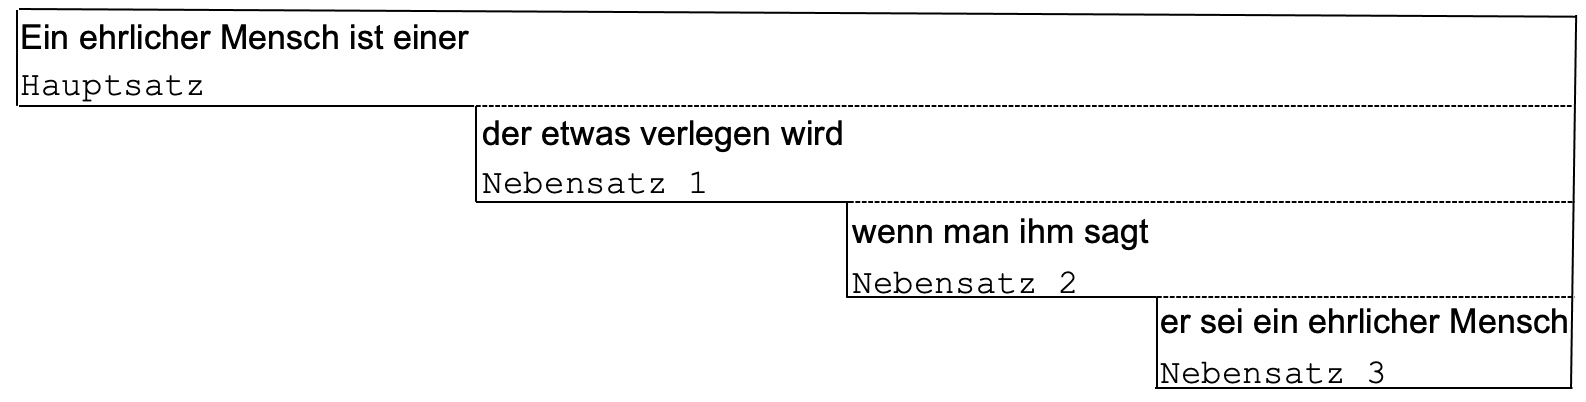
\includegraphics[width=12cm]{figures/Satzbild_Frisch.jpeg}
    %% Abbildung 


\noindent\resizebox{\textwidth}{!}{
	
	\begin{tabular}{  llll |}
		
		\hline
		\multicolumn{1}{ | l }{\makecell[l]{Ein ehrlicher Mensch ist einer \\ \small{\textcolor{gray}{Hauptsatz}}}}  &&& \\ \cline{1-1} \sbdashline{2-4}
		
		& \multicolumn{1}{ | l }{\makecell[l]{der etwas verlegen wird \\ \small{\textcolor{gray}{Nebensatz 1}}}}  && \\ \cline{2-2} \sbdashline{3-4}
		
		&& \multicolumn{1}{ | l }{\makecell[l]{wenn man ihm sagt \\ \small{\textcolor{gray}{Nebensatz 2}}}} & \\ \cline{3-3} \sbdashline{4-4}
		
		&&& \multicolumn{1}{ | l | }{\makecell[l]{er sei ein ehrlicher Mensch \\ \small{\textcolor{gray}{Nebensatz 3}}}} \\ \cline{4-4}
		
	\end{tabular}
}

	

	



    \caption{Satzbild zu (\ref{ea:FrischSatz_2})}
    \label{Abb:Satzbild_Frisch}
\end{figure}

Der Satz beginnt mit dem Hauptsatzgerüst als Teilsatz \textit{ein ehrlicher Mensch ist einer}. In diesen ist der erste komplexe Nebensatz \textit{der etwas verlegen wird, wenn man ihm sagt, er sei ein ehrlicher Mensch} als Attribut zu \textit{einer} integriert. Vom ersten Nebensatz hängt der zweite Nebensatz \textit{wenn man ihm sagt} ab. Dieser sättigt keine Valenzstelle des übergeordneten Prädikats \textit{etwas verlegen wird} (im Sinne von \gq{peinlich berührt werden}), sondern drückt als konditionales Satzadverbial die Bedingung für das Verlegen-Werden-Szenario aus. Der dritte Nebensatz \textit{er sei ein ehrlicher Mensch} sieht zwar durch Verbzweitstellung wie ein Hauptsatz aus. Aber er ist dem zweiten Nebensatz untergeordnet (verkappter Nebensatz). Denn er füllt als Satzobjekt die zweite Valenzstelle des übergeordneten Prädikats \textit{sagt}. 

Zu beachten ist, dass die jeweils tiefer eingebetteten Nebensätze auf höherer Ebene strukturell noch nicht sichtbar sind. Dies zeigt der Voranstellungstest. Der erste Nebensatz ist mit allen tiefer eingebetteten Nebensätzen zusammen mit dem Bezugswort \textit{einer} ein Satzglied im Hauptsatz (\ref{ea:NeSa123_Top}).

\ea \label{ea:NeSa123_Top} \textit{Einer, der etwas verlegen wird, wenn man ihm sagt, er sei ein ehrlicher Mensch}, ist ein ehrlicher Mensch.
\z 


Die Einbettungsebenen werden schrittweise pro Tabellenspalte erfasst. Die Struktur des Hauptsatzes wird ausgehend vom Hauptprädikat in der ersten Spalte analysiert. Das Hauptprädikat wird von der Kopula \textit{ist} in der linken Satzklammer gebildet. Kopulaverben sind zweiwertig und verlangen nach einem Subjekt und einem Subjektsprädikativ als semantisches Zentrum des Prädikats. Da es sich bei \textit{ein ehrlicher Mensch} und \textit{einer, der etwas verlegen wird, wenn man ihm sagt, er sein ein ehrlicher Mensch} um zwei NPs im Nominativ handelt, ist rein formal nicht klar, welche NP das Subjekt und welche das Subjektsprädikativ ist. Im Abschnitt~\ref{subsection:SP und OP} wurde die Funktion der Kopula als Behauptung einer Eigenschafts- oder Klassenzugehörigkeit beschrieben. In dem Satz (\ref{ea:FrischSatz_2}) wird behauptet, dass \textit{einer, der etwas verlegen wird, wenn man ihm sagt, er sei ein ehrlicher Mensch} in die Klasse \textit{ein ehrlicher Mensch} gehört. Folglich bestimmen wir \textit{ein ehrlicher Mensch} als Subjektsprädikativ und \textit{einer, der etwas verlegen wird, wenn man ihm sagt, er sein ehrlicher Mensch} als Subjekt. Diese Analyse wird durch die Umformung mit \textit{gelten als} in (\ref{ea:gelten_als_SP_statt_sein}) bestätigt. Denn mit \textit{gelten} wird das Subjektsprädikativ formal durch \textit{als} gekennzeichnet.

\ea \label{ea:gelten_als_SP_statt_sein} Als ein ehrlicher Mensch gilt einer, der etwas verlegen wird, wenn man ihm sagt, er sei ein ehrlicher Mensch.
\z 

Auch auf der ersten Nebensatz-Ebene bildet ein Kopulaverb, hier \textit{wird}, das Prädikat. Dieses verlangt nach einem Subjekt und einem Subjektsprädikativ. Das Relativpronomen \textit{der} fungiert als Subjekt und \textit{etwas verlegen} als Subjektsprädikativ. Denn es wird behauptet, dass die Eigenschaft \textit{etwas verlegen} auf \textit{der} zutrifft. Der Nebensatz \textit{wenn man ihm sagt, er sei ein ehrlicher Mensch} bildet auf der ersten Nebensatz-Ebene ein Satzglied. Für den Voranstellungstest formen wir den übergeordneten Nebensatz in einen Verbzweitsatz um (\ref{ea:NeSa23_Top}).

\ea \label{ea:NeSa23_Top} \textit{Wenn man ihm sagt, er sein ein ehrlicher Mensch}, wird er etwas verlegen.
\z 

Dieser Nebensatz sättigt keine Valenzstelle, sondern fungiert als konditionales Adverbial.

Der zweite Nebensatz wird mit der Subjunktion \textit{wenn} eingeleitet. Da Subjunktionen weder Satzglied noch Attribut sind, wird in der Tabelle ein Strich gemacht. Die Verbform \textit{sagt} bildet das Prädikat. Ausgehend von seiner Valenz bestimmen wir \textit{man} als dessen Subjekt, \textit{ihm} als Dativobjekt und den verkappten Nebensatz als Satzobjekt. Denn dieser sättigt die Valenzstelle für das, was gesagt wird. Da es sich um ein Satzglied handelt, ist der verkappte Nebensatz bei Umformung des übergeordneten Neben- in einen Hauptsatz voranstellbar (\ref{ea:NeSa3_Top}).

\ea \label{ea:NeSa3_Top} \textit{Er sei ein ehrlicher Mensch}, sagt man ihm.
\z 

Auf der dritten Nebensatz-Ebene wird die interne Struktur des letzten Nebensatzes analysiert. Die Konjunktivform \textit{sei} bildet als Kopula das Prädikat. Das Pronomen \textit{er} fungiert als Subjekt und \textit{ein ehrlicher Mensch} als Subjektsprädikativ.  

Die Analyse wird in der Tabelle~\ref{tab:Frisch_Satz} gezeigt.


\begin{table}
  \centering
  \resizebox{\textwidth}{!}{
  \begin{tabular}{l|l|l|l|l}
   % \lsptoprule
     & Hauptsatz &  1. NeSa-Ebene & 2. NeSa-Ebene  & 3. NeSa-Ebene \\
    \hline
    \textit{Ein} & \multirow{2}{*}{Subjekts-} &  & & \\
    \textit{ehrlicher} & \multirow{2}{*}{prädikativ} & & & \\
    \textit{Mensch} & & & \\ \cline{2-2}
    \textit{ist} & Prädikat  & & & \\ \cline{2-2}
    \textit{einer,} & \multirow{14}{*}{Subjekt} & & \\ \cline{3-3}
    \textit{der} & & Subjekt & &  \\ \cline{3-3}
    \textit{etwas} & & \multirow{1}{*}{Subjekts-} & &\\ 
    \textit{verlegen} & & \multirow{1}{*}{prädikativ} & & \\ \cline{3-3}
    \textit{wird,} & & Prädikat & & \\ \cline{3-4}
    \textit{wenn} & & \multirow{9}{*}{Adverbial} & -- & \\ \cline{4-4}
    \textit{man} & & & Subjekt & \\ \cline{4-4}
    \textit{ihm} & & & Dativobjekt & \\ \cline{4-4}
    \textit{sagt,} & & & Prädikat & \\ \cline{4-5}
    \textit{er} & & & \multirow{5}{*}{Satzobjekt} & Subjekt \\ \cline{5-5}
    \textit{sei} & & & & Prädikat \\ \cline{5-5}
    \textit{ein} & & & & \multirow{2}{*}{Subjekts-} \\ 
    \textit{ehrlicher} & & & & \multirow{2}{*}{prädikativ} \\ 
    \textit{Mensch.} & & & & \\
    \hline 
  %  \lspbottomrule
  \end{tabular}
  }
  \caption{Frisch-Satz}
  \label{tab:Frisch_Satz}
\end{table}


Nun zur Attribut-Ebene: Auf der obersten Ebene ist \textit{ehrlich} ein Adjektivattribut zu \textit{Mensch} und der Nebensatz \textit{der etwas verlegen wird, wenn man ihm sagt, er sei ein ehrlicher Mensch} ist ein Relativsatzattribut zu dem Indefinitpronomen \textit{einer}. 

Auf der ersten Nebensatz-Ebene kann \textit{etwas} im Sinne von \textit{ein bisschen} als Attribut zu dem Adjektiv \textit{verlegen} bestimmt werden. In Analogie zu dem Adverb \textit{sehr} kann es als von der Satzgliedebene abgeleitetes Adverbattribut bezeichnet werden.\footnote{Alternativ kann \textit{etwas} im Sinne von \textit{ein bisschen} als NP analysiert werden. Dann wäre aus dem adverbialen Akkusativ (\textit{etwas}/\textit{den ganzen Tag schlafen}) ein nominales Akkusativattribut geworden.} 

Auf der dritten Nebensatz-Ebene ist wieder \textit{ehrlich} ein Adjektivattribut zu \textit{Mensch}.


\subsection{Beispiel 2}\label{subsection:Bsp2}

Der nächste Satz stammt von Hans Mayer. Auch hier gibt es drei Nebensatz-Ebenen. Das Hauptsatzgerüst und der zweite Nebensatz sind jedoch durch andere Nebensätze \gq{unterbrochen}. Sie sind diskontinuierlich.

\ea \label{ea:Mayer_Satz} Dass sich diese junge Bundesrepublik, aus Rücksichten immer auf Wählerstimmen, nicht dazu entschließen konnte, die verjagten Emigranten, soweit sie noch lebten, zur Rückkehr aufzufordern, gehört, wie ich heute deutlicher spüre als noch vor Jahren, zu den Erbsünden dieses deutschen Teilstaates.\footnote{Hans Mayer: \textit{Wendezeiten}. Frankfurt am Main: Suhrkamp, 1993, S. 50.}
\z 

Erstellen Sie zuerst das Satzbild. Führen Sie danach die Satzgliedanalyse im Tabellenformat durch. Bestimmen Sie im Anschluss daran die Attributrelationen (Attributtyp und Bezugswort).


Kommen wir nun zu den Lösungen: Das Hauptprädikat \textit{gehört} erkennen wir an der Zweitstellung. Das Hauptsatzgerüst lautet \textit{gehört zu den Erbsünden dieses deutschen Teilstaates}. Der erste Nebensatz \textit{dass sich diese junge Bundesrepublik, aus Rücksichten immer auf Wählerstimmen, nicht dazu entschließen konnte} ist direkt dem Hauptsatzprädikat \textit{gehört} untergeordnet, da es der Kern seines Subjekts ist. Der zweite Nebensatz \textit{die verjagten Emigranten zur Rückkehr aufzufordern} hängt vom ersten ab. Denn er drückt das Objekt von \textit{auffordern} aus. Der zweite Nebensatz wird vom dritten Nebensatz \textit{soweit sie noch lebten} unterbrochen. Er hängt vom zweiten Nebensatz ab, denn er drückt die Bedingung dafür aus, unter der die Aufforderung gilt. Der vierte Nebensatz \textit{wie ich heute deutlicher spüre als noch vor Jahren} hängt direkt vom Hauptsatz ab und unterbricht diesen. Er drückt einen Kommentar des Sprechers zur Aussage des Hauptsatzes aus. Die Einbettungsebenen stellen wir in der Abbildung~\ref{Abb:Satzbild_Mayer} im Satzbild\is{Satzbild} dar. 

\begin{figure}
    \centering
    %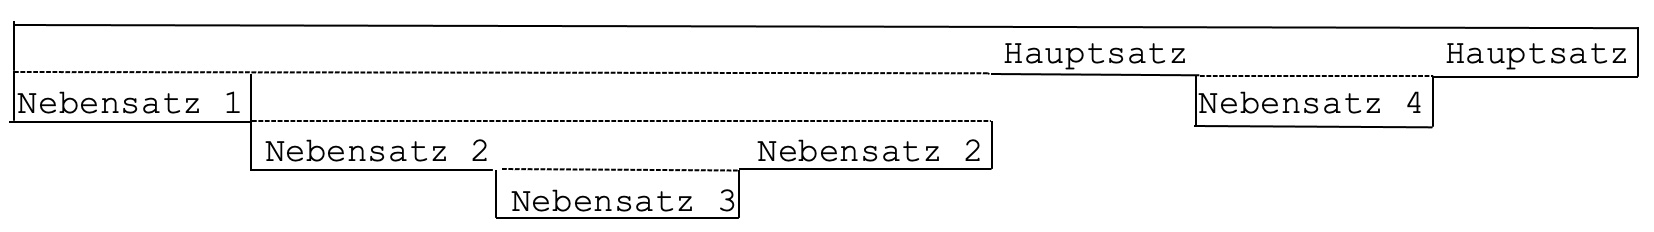
\includegraphics[width=12.5cm]{figures/Satzbild_Mayer.jpg}
    %% Abbildung 


\noindent\resizebox{\textwidth}{!}{
	
	\begin{tabular}{ p{2cm} p{2cm} p{2cm} p{2cm} p{2cm} p{2cm} p{2cm} }
		
		\hline
		
		\multicolumn{1}{ | l}{} & & & & \multicolumn{1}{ l}{\makecell{\small\textcolor{gray}{Hauptsatz}}} & & \multicolumn{1}{ l | }{\makecell{\small\textcolor{gray}{}}} \\ \sbdashline{1-4} \cline{5-5} \sbdashline{6-6} \cline{7-7}
		
		\multicolumn{1}{ | l  }{\makecell{\small\textcolor{gray}{Nebensatz 1}}} & & & \multicolumn{1}{ l | }{} & &
		\multicolumn{1}{ | l | }{\makecell{\small\textcolor{gray}{Nebensatz 4}}} & \\ \cline{1-1} \sbdashline{2-4} \cline{6-6}
		
		& \multicolumn{1}{ | l }{\makecell{\small\textcolor{gray}{Nebensatz 2}}} & &  \multicolumn{1}{ l | }{\makecell{\small\textcolor{gray}{}}} & & & \\ \cline{2-2} \sbdashline{3-3} \cline{4-4}

		& & \multicolumn{1}{ | l | }{\makecell{\small\textcolor{gray}{Nebensatz 3}}} & & & & \\ \cline{3-3} 
			
	\end{tabular}
}

	

    \caption{Satzbild zu (\ref{ea:Mayer_Satz})}
    \label{Abb:Satzbild_Mayer}
\end{figure}

Der Nebensatz im Vorfeld ist zusammen mit den in ihn eingebetteten Nebensätzen \textit{dass sich diese junge Bundesrepublik, aus Rücksichten immer auf Wählerstimmen, nicht dazu entschließen konnte, die verjagten Emigranten, soweit sie noch lebten, zur Rückkehr aufzufordern} das Subjekt des Hauptprädikats \textit{gehört}. Denn er sättigt die erste vom Verb geforderte Ergänzung. Wird sie durch eine NP ausgedrückt, muss sie im Nominativ stehen. Das zeigt die Pronominalisierung des Subjekts durch \textit{das} (\ref{ea:Mayer_Satz_SubjPrn}).

\ea \label{ea:Mayer_Satz_SubjPrn} \textit{Das} gehört, wie ich heute deutlicher spüre als noch vor Jahren, zu den Erbsünden dieses deutschen Teilstaates.
\z 

Ebenfalls als Satzglied innerhalb des Satzganzen fungiert der Nebensatz \textit{wie ich heute deutlicher spüre als noch vor Jahren}. Deshalb kann er, anders als weiterführende Nebensätze, vorangestellt werden (\ref{ea:Mayer_Satz_KAdv_Top}).

\ea \label{ea:Mayer_Satz_KAdv_Top} \textit{Wie ich heute deutlicher spüre als noch vor Jahren}, gehört zu den Erbsünden dieses deutschen Teilstaates, dass sich diese junge Bundesrepublik, aus Rücksichten immer auf Wählerstimmen, nicht dazu entschließen konnte, die verjagten Emigranten, soweit sie noch lebten, zur Rückkehr aufzufordern.
\z 

Dieser Nebensatz sättigt keine Valenzstelle. Durch ihn kommentiert der Schreiber das vom Hauptprädikat ausgedrückte Gehören-Szenario in seinem Geltungsbereich. Es geht um eine so gespürte Tatsache. Wir bestimmen den Nebensatz als Kommentaradverbial (vgl. Abschnitt~\ref{subsection:Adverbial}). Er kann so umgeformt werden, dass er als Hauptsatz den ursprünglichen Haupt- jetzt als Nebensatz einbettet (\ref{ea:Mayer_Satz_KGlied_HS}). Er ist alleine antwortfähig (\ref{ex:Mayer_Satz_KGlied_antwort}) und nicht vom Hauptsatz aus erfragbar (\ref{ex:Mayer_Satz_KGlied_Frage}).

\ea \label{ea:Mayer_Satz_KAdv_Tests}
\ea \label{ea:Mayer_Satz_KGlied_HS} \textit{Ich spüre heute deutlicher als noch vor Jahren}, dass es zu den Erbsünden dieses deutschen Teilstaates gehört, dass sich diese junge Bundesrepublik, aus Rücksichten immer auf Wählerstimmen, nicht dazu entschließen konnte, die verjagten Emigranten, soweit sie noch lebten, zur Rückkehr aufzufordern.
\ex \label{ex:Mayer_Satz_KGlied_antwort} Gehört es zu den Erbsünden dieses deutschen Teilstaates, dass sich diese junge Bundesrepublik, aus Rücksichten immer auf Wählerstimmen, nicht dazu entschließen konnte, die verjagten Emigranten, soweit sie noch lebten, zur Rückkehr aufzufordern? – \textit{Ich spüre das heute deutlicher als vor Jahren} (\textit{so}).
\ex \label{ex:Mayer_Satz_KGlied_Frage} *Wie gehört es zu den Erbsünden dieses deutschen Teilstaates, dass sich diese junge Bunderepublik, aus Rücksichten immer auf Wählerstimmen, nicht dazu entschließen konnte, die verjagten Emigranten, soweit sie noch lebten, zur Rückkehr aufzufordern? – \textit{Ich spüre das heute deutlicher als vor Jahren} (\textit{so}). 
\z 
\z 

Das Prädikat dieses Nebensatzes bildet die Verbform \textit{spüre}. Das Pronomen \textit{ich} fungiert als dessen Subjekt. Ausgehend von der zweiwertigen Valenz ist ein Akkusativobjekt erwartbar. Sprachlich wird dieses aber nicht ausgedrückt. Denn \textit{wie} kodiert normalerweise eine modale Adverbialfunktion. Es gibt zwei Möglichkeiten der Analyse. Entweder verstehen wir das als Adverbial angelegte Satzglied \textit{wie} im Sinne von \gq{was ich heute deutlicher spüre}.\footnote{Dieses Verständnis kann auch bei entsprechendem \textit{wie}-Nebensatz gelten: \textit{Ich spüre, dass/wie es regnet.}} Es gerät in den Sog der offenen Valenzstelle und sättigt diese, als wäre es ein Akkusativobjekt. Oder wir verstehen \textit{spüren} hier absolut als eine Tätigkeit, nicht als Handlung, also einwertig. Dann fungiert \textit{wie}, wie angelegt, als modales Adverbial im Sinne von \gq{auf eine unbestimmte Art spüren}. Wir entscheiden uns für diese Bestimmung, da sie keine Umfunktionierung nötig macht. Das Satzglied \textit{deutlicher als noch vor zehn Jahren} fungiert als modales Adverbial und \textit{heute} als temporales Adverbial. 

Kommen wir nun zu den anderen Nebensätzen. Der Nebensatzkomplex im Vorfeld besteht aus drei Nebensätzen. Der erste Nebensatz lautet \textit{dass sich diese junge Bundesrepublik, aus Rücksichten immer auf Wählerstimmen, nicht dazu entschließen konnte}. Ausgehend von der Valenz von \textit{sich entschließen konnte} bestimmen wir die NP im Nominativ \textit{diese junge Bundesrepublik} als Subjekt und \textit{dazu} als Präpositionalobjekt, worauf weiter unten noch einmal eingegangen wird. Bei \textit{nicht} handelt es sich weder um ein Satzglied noch um den attributiven Teil eines Satzglieds. Dies wird in der Analyse durch einen Strich gekennzeichnet. 

Bei \textit{aus Rücksichten immer auf Wählerstimmen} handelt es sich um ein eingeschobenes kausales Adverbial, das den Grund dafür angibt, warum sich diese Bundesrepublik nicht zu etwas entschließen konnte. Es bezieht sich direkt auf das Prädikat \textit{sich entschließen konnte}. Dies bestätigt der Voranstellungstest in (\ref{ex:Mayer_Satz_aus_Rücksichten_Top}), wenn der einbettende Nebensatz in einen Hauptsatz umformuliert wird (\ref{ea:Mayer_Satz_aus_Rücksichten_HS}). 

\ea \label{ea:Mayer_Satz_aus_Rücksichten_Top_HS} 
\ea \label{ea:Mayer_Satz_aus_Rücksichten_HS} Diese junge Bundesrepublik konnte sich, aus Rücksichten immer auf Wählerstimmen, nicht dazu entschließen.
\ex \label{ex:Mayer_Satz_aus_Rücksichten_Top} \textit{Aus Rücksichten immer auf Wählerstimmen} konnte sich diese junge Bundesrepublik nicht dazu entschließen.
\z 
\z 

Das kausale Adverbial \textit{aus Rücksichten immer auf Wählerstimmen} ist komplex, kann aber nicht im Rahmen der Satzgliedanalyse \gq{aufgedröselt} werden. Es besteht nämlich intern nicht aus Satzgliedern, da es kein Prädikat gibt.

Die Proform \textit{dazu} im ersten Nebensatz zeigt wie ein Korrelat (vgl. Abschnitt~\ref{subsection:Korrelat}) die Sättigung der zweiten Valenzstelle des Prädikats an. Das Prädikat \textit{sich entschließen konnte} fordert eine zweite Ergänzung in Form einer PP mit \textit{zu}. Darüber hinaus kann \textit{dazu} mit Betonung auf \textit{da} auf den als Attribut fungierenden Nebensatzkomplex \textit{die verjagten Emigranten, soweit sie noch lebten, zur Rückkehr aufzufordern} zeigen. Als Test gilt wieder die gemeinsame Voranstellbarkeit (\ref{ea:ea:Mayer_Satz_dazu_zuINF_Top}) bei Umformung in einen Hauptsatz.

\ea \label{ea:ea:Mayer_Satz_dazu_zuINF_Top} \textit{Dazu, die Emigranten, soweit sie noch lebten, zur Rückkehr aufzufordern}, konnte sich diese junge Bundesrepublik nicht entschließen.
\z 

In diesem Fall ist \textit{dazu} der Kern des Präpositionalobjekts, zu dem der Nebensatz als Attribut gehört. Wird hingegen \textit{dazu} mit Betonung auf \textit{zu} gelesen, dann müsste es als Korrelat zum Satzobjekt \textit{die Emigranten, soweit sie noch lebten, zur Rückkehr aufzufordern} analysiert werden. Beide Analysen wären korrekt.  

Die zweite nebensatzähnliche Struktur \textit{die Emigranten zur Rückkehr aufzufordern} wird durch die Infinitiv-Konstruktion (vgl. \ref{subsection:NebensatzähnlicheK}) mit \textit{aufzufordern} als Prädikat gebildet. Da Infinitive die erste verbale Ergänzung im Nominativ nicht ausdrücken können, gibt es kein Subjekt. Der Infinitiv \textit{aufzufordern} verlangt jedoch nach einer Ergänzung im Akkusativ und nach einer Ergänzung mit der Präposition \textit{zu}. Folglich fungieren \textit{die Emigranten} als Akkusativobjekt und \textit{zur Rückkehr} als Präpositionalobjekt.

Die Infinitiv-Konstruktion ist durch den Nebensatz \textit{soweit sie noch lebten} unterbrochen. Der Begriff \textit{Einbettung} wird hier plastisch. Der dritte Nebensatz \textit{soweit sie noch lebten} liegt innerhalb der zweiten nebensatzähnlichen Konstruktion. Er sättigt keine Valenzstelle des einbettenden Prädikats \textit{aufzufordern}, sondern drückt als konditionales Adverbial die Bedingung für jene Aufforderung aus. Dass es sich um ein Adverbial und damit um ein Satzglied handelt, wird durch den Voranstellungstest in (\ref{ex:Mayer_Satz_soweit_Top}) bei Umformulierung in einen Hauptsatz (\ref{ea:ea:Mayer_Satz_soweit_in_HS}) untermauert.

\ea \label{ea:ea:Mayer_Satz_soweit_Top_HS} 
\ea \label{ea:ea:Mayer_Satz_soweit_in_HS} Diese junge Bundesrepublik forderte die Emigranten, soweit sie noch lebten, nicht zur Rückkehr auf.
\ex \label{ex:Mayer_Satz_soweit_Top} \textit{Soweit sie noch lebten}, forderte diese junge Bundesrepublik die Emigranten nicht zur Rückkehr auf.\footnote{Allerdings bekommt dieses Satzgefüge eine weitere Lesart, nämlich dass die Emigranten nicht zur Rückkehr aufgefordert wurden, weil sie noch lebten. Unser Weltwissen arbeitet bei der sinnvollen Interpretation mit. Im Präteritum \textit{soweit sie noch lebten} ergibt sich Plausibilität der konditionalen Kodierung durch kausale Interpretation.}
\z 
\z 

Das Zentrum des eingebetteten Nebensatzes bildet die Verbform \textit{lebten} als Prädikat. Es verlangt nach einer Ergänzung im Nominativ. Das Pronomen \textit{sie} sättigt diese Valenzstelle und fungiert als Subjekt. Durch \textit{noch} wird keine Valenzstelle gesättigt. Es drückt zeitliche Aspekte des Leben-Szenarios aus und ist somit ein temporales Adverbial. Die Subjunktion \textit{soweit} ist weder Satzglied noch Teil eines Satzglieds und wird daher nicht bestimmt. 

Die Satzgliedanalyse wird in der Tabelle~\ref{tab:Mayer_Satz} dargestellt. Die Spalten entsprechen wieder den Ebenen des Satzbildes, wenn dieses um 90 Grad nach links gedreht würde.

\begin{table}
%\scriptsize  
  \centering
  \resizebox{\textwidth}{!}{
  \begin{tabular}{l|l|l|l|l}
   % \lsptoprule
     &  Hauptsatz  &  1. NeSa-Ebene &  2. NeSa-Ebene &  3. NeSa-Ebene \\
    \hline
    \textit{Dass} & \multirow{29}{*}{Subjekt} & -- & & \\ \cline{3-3}
    \textit{sich} & & Prädikat & & \\ \cline{3-3}
    \textit{diese} & & \multirow{3}{*}{Subjekt} & & \\  
    \textit{junge} &  & & & \\ 
    \textit{Bundesrepublik,} & & & & \\ \cline{3-3}
    \textit{aus} & & \multirow{5}{*}{Adverbial} \\
    \textit{Rücksichten} & & & & \\
    \textit{immer} & & & & \\ 
    \textit{auf} & & & & \\ 
    \textit{Wählerstimmen,} & & & & \\ \cline{3-3}
    \textit{nicht} & & -- & & \\ \cline{3-3}
    \textit{dazu} & & Präpositionalobjekt & & \\ \cline{3-3}
    \textit{entschließen} & & \multirow{2}{*}{Prädikat} & & \\ 
    \textit{konnte,} & & & & \\ \cline{3-4}
    \textit{die} & & \multirow{10}{*}{Präpositionalobjekt} & \multirow{3}{*}{Akkusativobjekt} & \\
    \textit{verjagten} & &  &  & \\
    \textit{Emigranten,} & & & & \\ \cline{4-5}
    \textit{soweit} & & & \multirow{4}{*}{Adverbial} & -- \\ \cline{5-5}
    \textit{sie} & & & & Subjekt \\ \cline{5-5}
    \textit{noch} & & & & Adverbial \\ \cline{5-5}
    \textit{lebten,} & & & & Prädikat \\ \cline{4-5}
    \textit{zur} & & & \multirow{2}{*}{Präpositionalobjekt} & \\
    \textit{Rückkehr} & & & & \\ \cline{4-4}
    \textit{aufzufordern,} & & & Prädikat & \\ \cline{2-4} 
    \textit{gehört,} & Prädikat & -- & & \\ \cline{2-3}
    \textit{wie} & \multirow{10}{*}{Kommentaradverbial} & Adverbial & & \\ \cline{3-3}
    \textit{ich} & & Subjekt & & \\ \cline{3-3}
    \textit{heute} & & Adverbial 1 & & \\ \cline{3-3}
    \textit{deutlicher} & & Adverbial 2 & & \\ \cline{3-3}
    \textit{spüre} & & Prädikat & & \\ \cline{3-3}
    \textit{als} & & \multirow{5}{*}{Adverbial 2} & & \\ 
    \textit{noch} & & & & \\
    \textit{vor} & & & & \\ 
    \textit{zehn} & & & & \\ 
    \textit{Jahren,} & & & & \\ \cline{2-3}
    \textit{zu} & \multirow{6}{*}{Präpositionalobjekt} & & & \\ 
    \textit{den} & & & & \\
    \textit{Erbsünden} & & & & \\ 
    \textit{dieses} & & & & \\ 
    \textit{deutschen} & & & & \\ 
    \textit{Teilstaates.} & & & & \\
    \hline 
   % \lspbottomrule
  \end{tabular}
  }
  \caption{Diskontinuierliche Sätze durch Einbettung}
  \label{tab:Mayer_Satz}
\end{table}

Kommen wir nun zu den Attributen: Auf der ersten Ebene ist innerhalb des Präpositionalobjektes die NP \textit{dieses deutschen Teilstaates} ein Genitivattribut zu \textit{Erbsünde}. Innerhalb des Attributs \textit{dieses deutschen Teilstaates} ist \textit{deutschen} ein Adjektivattribut zu \textit{Teilstaates}.

Auf der ersten Nebensatz-Ebene ist die PP \textit{auf Wählerstimmen} ein Präpositionalattribut zu \textit{Rücksichten}. Das Adverb \textit{immer} fungiert als Adverbphrase (vgl. Abschnitt~\ref{section:Adverbphrase}) typischerweise als Adverbial. Da es hier kein Prädikat gibt, ist diese Funktion ausgeschlossen. Analog zu Fokuspartikeln wie \textit{besonders} in \textit{besonders auf Wählerstimmen} analysieren wir \textit{immer} als Adverbattribut zu der PP \textit{auf Wählerstimmen}.\footnote{Die syntaktische Attributbeziehung innerhalb von \textit{immer auf Wählerstimmen} ist analog zur Modifikation lokaler PPs wie \textit{direkt vor der Kreuzung} zu verstehen.}

Da wir \textit{dazu} als Kern des Präpositionalobjekts (und nicht, was auch möglich wäre, als Korrelat zum Satzobjekt) analysiert haben, fungiert die Infinitivkonstruktion \textit{die verjagten Emigranten, soweit sie noch lebten, zur Rückkehr aufzufordern} als Attribut zu \textit{dazu}. Auch hier handelt es sich um eine Umfunktionierung von der Satzgliedebene auf die Ebene der Wortgruppe.

Die Vergleichsphrase \textit{als noch vor zehn Jahren} ist ein Attribut der Komparativform \textit{deutlicher} und damit Teil des Adverbials. 

Auf der zweiten Nebensatz-Ebene ist \textit{verjagten} ein Adjektivattribut zu \textit{Emigranten}. Auf der dritten Nebensatz-Ebene gibt es keine Attribute.


\subsection{Beispiel 3}\label{subsection:Bsp3}

Nun analysieren wir den folgenden Satz aus \textit{Max und Moritz} von Wilhelm Busch.

\ea \label{ea:Busch_Satz} Als die gute Witwe Bolte sich von ihrem Schmerz erholte, dachte sie so hin und her, dass es wohl das beste wär, die Verstorbenen, die hienieden schon so frühe abgeschieden, ganz im Stillen und in Ehren gut gebraten zu verzehren.\footnote{Wilhelm Busch: \textit{Max und Moritz. Eine Bubengeschichte in sieben Streichen}. [1865]. Göttingen: Literatur- und Wissenschaftsverlag, 2019, S. 7.}
\z 

Erstellen Sie zuerst das Satzbild. Führen Sie danach die Satzgliedanalyse im Tabellenformat durch. Bestimmen Sie im Anschluss daran die Attributrelationen (Attributtyp und Bezugswort).


Kommen wir nun zu den Lösungen: Das Hauptprädikat \textit{dachte} erkennen wir an der Zweitstellung. Das Hauptsatzgerüst lautet \textit{dachte sie so hin und her}. Der erste Nebensatz \textit{als die gute Witwe Bolte sich von ihrem Schmerz erholte} ist direkt dem Hauptsatz untergeordnet, da er die Zeit des \textit{Denkens} ausdrückt. Den Inhalt des \textit{Denkens} drückt der zweite Nebensatz \textit{dass es wohl das beste wär} aus und ist somit direkt dem Hauptsatzprädikat untergeordnet. Der dritte Nebensatz \textit{die Verstorbenen ganz im Stillen und in Ehren gut gebraten zu verzehren} ist direkt dem zweiten Nebensatz untergeordnet. Denn er drückt das aus, was das \textit{beste wär}. Der vierte Nebensatz \textit{die hienieden schon so frühe abgeschieden} unterbricht den dritten Nebensatz, in den er eingebettet ist. Denn er hängt direkt von \textit{die Verstorbenen} ab.

Die Einbettungsebenen der Nebensätze stellen wir in der Abbildung~\ref{Abb:Satzbild_Max_Moritz} im Satzbild\is{Satzbild} dar.

\begin{figure}
    \centering
    %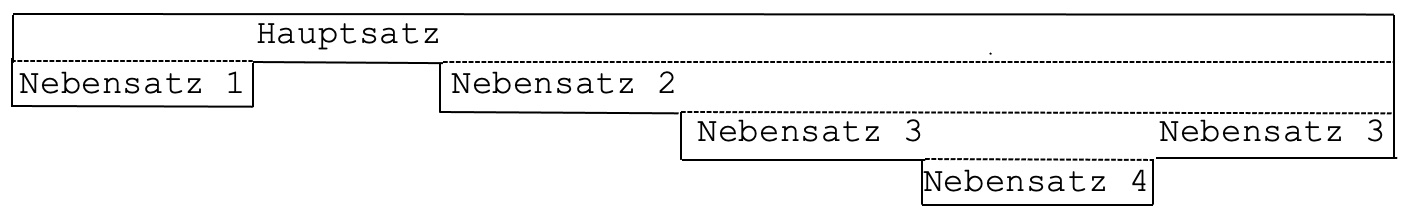
\includegraphics[width=12.5cm]{figures/Satzbild_Max_Moritz.jpeg}
    %% Abbildung 


\noindent\resizebox{\textwidth}{!}{
	
	\begin{tabular}{ p{2cm} p{2cm} p{2cm} p{2cm} p{2cm} p{2cm} }
		
		\hline
		
		\multicolumn{1}{ | l}{} &
		\multicolumn{1}{ l }{\makecell[l]{\small\textcolor{gray}{Hauptsatz}}} & & & &
		\multicolumn{1}{ l | }{} \\ 
		\sbdashline{1-1} \cline{2-2} \sbdashline{3-6} 
		
		\multicolumn{1}{ | l | }{\makecell[l]{\small\textcolor{gray}{Nebensatz 1}}} & &  
		\multicolumn{1}{ | l  }{\makecell[l]{\small\textcolor{gray}{Nebensatz 2}}} & & & 
		\multicolumn{1}{ l | }{} \\
		 \cline{1-1} \cline{3-3} \sbdashline{4-6} 
		 
		& & &  \multicolumn{1}{ | l }{\makecell[l]{\small\textcolor{gray}{Nebensatz 3}}} & &  
		\multicolumn{1}{ l | }{\makecell[l]{\small\textcolor{gray}{}}} \\
		 \cline{4-4} \sbdashline{5-5}  \cline{6-6}
		 
		 & & & & \multicolumn{1}{ | l | }{\makecell[l]{\small\textcolor{gray}{Nebensatz 4}}} & \\
		 \cline{5-5} 
			
	\end{tabular}
}


    \caption{Satzbild zu (\ref{ea:Busch_Satz})}
    \label{Abb:Satzbild_Max_Moritz}
\end{figure}

Das Prädikat des Hauptsatzes ist \textit{dachte}. Das Pronomen \textit{sie} sättigt als NP im Nominativ die erste Valenzstelle von \textit{dachte} und fungiert als Subjekt. Die koordinierte Adverbphrase \textit{so hin und her} sättigt keine Valenzstelle, sondern drückt im weiteren Sinne eine Art und Weise des Denkens aus.\footnote{Es handelt sich um eine bildliche Übertragung von Bewegungssituationen wie \textit{hin und her laufen}. Die ursprüngliche Bedeutung \gq{ständig die Richtung wechselnd} wird metaphorisch als \gq{gründlich, alles erwägend} verstanden}. Es handelt sich um ein modales Adverbial. Die Erststellfähigkeit (\ref{ea:Busch_Satz_hinher_Top}) spricht für den Satzgliedstatus.

\ea \label{ea:Busch_Satz_hinher_Top} \textit{So hin und her} dachte sie, dass\ldots{} 
\z 

Denkbar wäre jedoch auch, \textit{hin} und \textit{her} als Teile des Prädikats zu bestimmen. Auch diese können vorangestellt werden. Dagegen spricht, dass es für sich genommen weder ein *\textit{Hindenken} noch ein *\textit{Herdenken} gibt. \textit{Hin und her} bildet eine im Satz bewegliche Phrase, die über Bewegungsverben hinaus metaphorisch gebraucht werden kann. Vor allem spricht gegen die Bestimmung als Prädikatsteil, dass \textit{hin und her} auch mit Verben, die bereits eine Partikel oder ein Präfix enthalten, gebraucht werden kann wie in \textit{etwas hin und her abwägen} oder \textit{etwas hin und her überlegen}.    
 
Das Hauptprädikat \textit{dachte} verlangt nach einer zweiten Ergänzung, die den Inhalt des Denkens typischerweise durch einen Nebensatz ausdrückt. Der Nebensatzkomplex \textit{dass es wohl das beste wär, die Verstorbenen, die hienieden schon so frühe abgeschieden, ganz im Stillen und in Ehren gut gebraten zu verzehren} sättigt diese Valenzstelle und ist damit ein Satzobjekt. Hierfür sprechen die gemeinsame Voranstellbarkeit (\ref{ea:Busch_Satz_Satzobj_Top}), die Pronominalisierbarkeit (\ref{ex:Busch_Satz_Satzobj_Pronomen}) und Erfragbarkeit durch ein Fragepronomen (\ref{ex:Busch_Satz_Satzobj_Frage}).

\ea \label{ea:Busch_Satz_Satzobj}
\ea \label{ea:Busch_Satz_Satzobj_Top} \textit{Dass es wohl das beste wär, die Verstorbenen, die hienieden schon so frühe abgeschieden, ganz im Stillen und in Ehren gut gebraten zu verzehren}, dachte die gute Witwe Bolte so hin und her, als sie sich von ihrem Schmerz erholte.\footnote{Innerhalb des Hauptsatzes muss jetzt das Subjekt \textit{sie} durch \textit{die gute Witwe Bolte} ersetzt werden. Denn das Pronomen \textit{sie} soll auf die referierende (in die Welt zeigende) NP \textit{die gute Witwe Bolte} verweisen. Dieses Verweisen vom Pronomen auf eine NP (Phorik) funktioniert nur, wenn das Pronomen und die NP nicht auf gleicher und wenn das Pronomen nicht auf einer höheren Strukturposition als die NP steht. Eine höhere Strukturposition bedeutet hier: Das Pronomen kann nicht aus dem Hauptsatz auf eine NP im folgenden Nebensatz verweisen: *\textit{sie dachte das so hin und her, als die gute Witwe Bolte sich von ihrem Schmerz erholte}. Wenn das Pronomen im Nebensatz und somit strukturtiefer steht, dann kann es auch bei Voranstellung (Thema-Stellung) auf die NP im Hauptsatz verweisen: \textit{als sie sich vom Schmerz erholte, dachte die gute Witwe Bolte das so hin und her}. Dieses Phänomen wird in der Linguistik unter dem Stichwort \textit{Koreferenz} diskutiert. Cf. \citet[93--104]{FanselowFelix1993} und \citet[109--115]{Welke1993}.} 
\ex \label{ex:Busch_Satz_Satzobj_Pronomen} Als die gute Witwe Bolte sich von ihrem Schmerz erholte, dachte sie \textit{das} so hin und her.
\ex \label{ex:Busch_Satz_Satzobj_Frage} \textit{Was} dachte die gute Witwe Bolte so hin und her,  als sie sich von ihrem Schmerz erholte?
\z 
\z 

Vor dem Hauptprädikat \textit{dachte} erwarten wir ein Satzglied. Der Nebensatz \textit{als die gute Witwe Bolte sich von ihrem Schmerz erholte} sättigt keine Valenzstelle von \textit{dachte}. Er drückt ein Szenario aus, das zeitgleich zum Szenario des Hauptsatzes stattfindet. Es handelt sich um ein temporales Adverbial. Das Reflexivpronomen ist Teil des Prädikats \textit{sich erholte}, denn es sättigt keine Valenzstelle (vgl. Abschnitt~\ref{subsection:Reflexiva}). Es ist zweiwertig. Die NP im Nominativ \textit{die gute Witwe Bolte} fungiert als Subjekt und die PP \textit{von ihrem Schmerz} als Präpositionalobjekt (vgl. Abschnitt~\ref{subsection:Pobj}).

Jetzt beschäftigen wir uns mit dem als Satzobjekt fungierenden Nebensatzkomplex: \textit{dass es wohl das beste wär, die Verstorbenen, die hienieden schon so frühe abgeschieden, ganz im Stillen und in Ehren gut gebraten zu verzehren}. Der erste Nebensatz \textit{dass es wohl das beste wär} enthält ein Korrelat. \textit{Es} zeigt an, dass ein Nebensatz in Objekt- oder Subjektfunktion folgt. Bei \textit{wär} handelt es sich um eine Konjunktivform (II) der Kopula \textit{sein}. Ihre Ergänzung ist das Subjektsprädikativ \textit{das beste}. Das Korrelat \textit{es} steht also im Nominativ und zeigt auf die folgende Infinitivkonstruktion in Subjektfunktion. Diese Funktion übernimmt der ganze folgende Komplex \textit{die Verstorbenen, die hienieden schon so frühe abgeschieden, ganz im Stillen und in Ehren gut gebraten zu verzehren}. Dass es sich in Bezug auf \textit{das beste sein} um \textit{ein} Satzglied handelt, zeigt bei Umformung in einen Hauptsatz (\ref{ea:Busch_Satz_beste_wär_Inf_HS}) die Voranstellung (\ref{ex:Busch_Satz_beste_wär_Inf_Top}).

\ea \label{ea:Busch_Satz_beste_wär_Inf}
\ea \label{ea:Busch_Satz_beste_wär_Inf_HS} Wohl wäre es das beste, die Verstorbenen, die hienieden schon so frühe abgeschieden, ganz im Stillen und in Ehren gut gebraten zu verzehren.
\ex \label{ex:Busch_Satz_beste_wär_Inf_Top} \textit{Die Verstorbenen, die hienieden schon so frühe abgeschieden, ganz im Stillen und in Ehren gut gebraten zu verzehren}, wäre wohl das beste.
\z 
\z 

Dass es sich bei \textit{es} tatsächlich um ein Subjekt-Korrelat und nicht um das Subjekt handelt, wird in (\ref{ex:Busch_Satz_beste_wär_Inf_Top}) deutlich. Bei Voranstellung des Subjektsatzes entfällt \textit{es}. 

Bei der Umformung in einen Hauptsatz (\ref{ea:Busch_Satz_beste_wär_Inf_HS}) haben wir \textit{wohl} ins Vorfeld gestellt. So sehen wir erstens, dass \textit{es} kein reiner Vorfeld-Platzhalter (vgl. Abschnitt~\ref{subsection:Vorfeld}) ist und dass dieses \textit{wohl} ein Satzglied ist. Wir bestimmen \textit{wohl} als Kommentaradverbial (vgl. Abschnitt~\ref{subsection:Adverbial}). Denn es räumt wie \textit{wahrscheinlich} oder \textit{bestimmt} Zweifel bezüglich der Geltung des gesamten Szenarios aus. Es kann in einen Hauptsatz umgeformt werden, der den ursprünglich einbettenden Satz zum Nebensatz macht (\ref{ea:Busch_Satz_beste_wär_wohl_HS}) und es ist nicht wie andere Adverbiale erfragbar (\ref{ex:Busch_Satz_beste_wär_wohl_*Frage}).


\ea \label{ea:Busch_Satz_beste_wär_wohl}
\ea [] {Es ist wohl so, dass es das beste wär, die Verstorbenen, die hienieden schon so frühe abgeschieden, ganz im Stillen und in Ehren gut gebraten zu verzehren.}\label{ea:Busch_Satz_beste_wär_wohl_HS}
\ex [*] {\textit{Wie} wäre es das beste, die Verstorbenen, die hienieden schon so frühe abgeschieden, ganz im Stillen und in Ehren gut gebraten zu verzehren?  -- Wohl.}\label{ex:Busch_Satz_beste_wär_wohl_*Frage}
\z 
\z 

Bei dem Subjekt \textit{die Verstorbenen, die hienieden schon so frühe abgeschieden, ganz im Stillen und in Ehren gut gebraten zu verzehren} handelt es sich um eine satzwertige \textit{zu}-Infinitiv-Konstruktion (vgl. Abschnitt~\ref{subsection:NebensatzähnlicheK}). Deren Prädikat bildet \textit{zu verzehren}. Da es sich um einen Infinitiv handelt, kann das mitzudenkende Subjekt formal nicht ausgedrückt werden. Die zweite, obligatorisch zu besetzende Valenzstelle von \textit{verzehren} wird durch \textit{die Verstorbenen, die hienieden schon so frühe abgeschieden} als Akkusativobjekt gesättigt. Dass es sich auf dieser Ebene um \textit{ein} Satzglied handelt, wird bei Umformung in einen Hauptsatz (\ref{ea:Busch_Satz_zu_verzehren_HS}) durch Voranstellung (\ref{ex:Busch_Satz_zu_verzehren_Top}) deutlich.

\ea \label{ea:Busch_Satz_zu_verzehren_HS_TOP}
\ea \label{ea:Busch_Satz_zu_verzehren_HS} Sie will die Verstorbenen, die hienieden schon so frühe abgeschieden, ganz im Stillen und in Ehren gut gebraten verzehren.
\ex \label{ex:Busch_Satz_zu_verzehren_Top} {Die Verstorbenen, die hienieden schon so frühe abgeschieden}, will sie ganz im Stillen und in Ehren gut gebraten verzehren.
\z 
\z 

Die koordinierten PPs \textit{ganz im Stillen und in Ehren} bilden ebenfalls ein Satzglied. Der Komplex ist voranstellbar (\ref{ea:Busch_Satz_zu_verzehren_im_Stillen_Top}) und erfragbar (\ref{ex:Busch_Satz_zu_verzehren_im_Stillen_Frage}).

\ea \label{ea:Busch_Satz_zu_verzehren_im_Stillen}
\ea \label{ea:Busch_Satz_zu_verzehren_im_Stillen_Top} \textit{Ganz im Stillen und in Ehren} will sie die Verstorbenen, die hienieden schon so frühe abgeschieden, gut gebraten verzehren.
\ex \label{ex:Busch_Satz_zu_verzehren_im_Stillen_Frage} \textit{Wie} will sie die Verstorbenen, die hienieden schon so frühe abgeschieden,  gut gebraten verzehren? -- Ganz im Stillen und in Ehren.
\z 
\z 

Der Komplex sättigt keine Valenzstelle von \textit{zu verzehren}. Er drückt die Art und Weise des Verzehren-Szenarios aus. Es handelt sich um ein modales Adverbial.

Bei \textit{gut gebraten} handelt es sich um eine satzwertige Partizipial-Konstruktion (vgl. Abschnitt~\ref{subsection:NebensatzähnlicheK}). Wir bestimmen sie als Satzglied. Dafür spricht ihre Voranstellbarkeit (\ref{ea:Busch_Satz_gut_gebraten_TOP}).

\ea \label{ea:Busch_Satz_gut_gebraten_TOP} \textit{Gut gebraten} will sie die Verstorbenen, die hienieden schon so frühe abgeschieden, verzehren.
\z 

Um welche Satzgliedfunktion handelt es sich? Die Partizipial-Konstruktion sättigt weder eine Valenzstelle des Prädikats \textit{zu verzehren} noch spezifiziert sie wie Adverbiale das Verzehren-Szenario. Sie weist dem Akkusativobjekt \textit{die Verstorbenen, die hienieden schon so frühe abgeschieden} die Eigenschaft \textit{gut gebraten} für die Zeit des Verzehrens zu. Diese Funktion kommt freien Prädikativen (vgl. Abschnitt~\ref{subsection:freiePräd}) zu. Hier handelt es sich um ein freies Objekstprädikativ. Der besondere Bezug zum Objekt zeigt sich in Stellungseigenschaften. Das freie Prädikativ folgt bei Nebensatzstellung typischerweise seinem Bezugswort. In (\ref{ea:Busch_Satz_gut_gebraten_Obj_Adjazenz}) folgt \textit{gut gebraten} dem Objekt. In (\ref{ex:Busch_Satz_gut_gebraten_Subj_Adjazenz}) müssten wir die Partizipial-Konstruktion als freies Subjektsprädikativ verstehen, also dass Witwe Bolte zum Zeitpunkt des Verzehrens gut gebraten ist.

\ea \label{ea:Busch_Satz_gut_gebraten_FP}
\ea \label{ea:Busch_Satz_gut_gebraten_Obj_Adjazenz} weil die gute Witwe Bolte die Verstorbenen \textit{gut gebraten} verzehren will.
\ex \label{ex:Busch_Satz_gut_gebraten_Subj_Adjazenz} weil die gute Witwe Bolte \textit{gut gebraten} die Verstorbenen verzehren will
\z 
\z 

Intern besteht das freie Prädikativ aus dem Prädikat \textit{gebraten} und dem nicht-valenzsättigenden Adverbial \textit{gut}.

Nun muss noch die Funktion des eingebetteten Nebensatzes \textit{die hienieden schon so frühe abgeschieden} bestimmt werden. Es handelt sich formal um einen elliptischen Relativsatz. Elliptisch ist er, weil das finite Hilfsverb \textit{sind} zum Perfektausdruck \textit{abgeschieden sind} in der Bedeutung von \textit{gestorben/verschieden sind} ausgelassen wurde. Seine Funktion ist die nähere Bestimmung von \textit{die Verstorbenen}. Er ist kein Satzglied, sondern als Attribut Teil des Akkusativobjekts, wofür auch die gemeinsame Voranstellung in (\ref{ex:Busch_Satz_zu_verzehren_Top}) spricht. Intern besteht er aus \textit{die} in Subjektfunktion, \textit{hienieden} als lokales Adverbial und \textit{schon so frühe} als temporales Adverbial zum Prädikat \textit{abgeschieden} (\textit{sind}). 

Die Satzgliedanalyse wird in der Tabelle~\ref{tab:Busch_Satz} dargestellt.

\begin{table}
%\scriptsize  
  \centering
  \resizebox{\textwidth}{!}{
  \begin{tabular}{l|l|l|l|l}
   % \lsptoprule
      &  Haupsatz  &  1. NeSa-Ebene  &  2. NeSa-Ebene  &  3. NeSa-Ebene  \\
    \hline
    \textit{Als} & \multirow{10}{*}{Adverbial} & -- & & \\ \cline{3-3}
    \textit{die} & & \multirow{3}{*}{Subjekt} & & \\ 
    \textit{gute} & & & & \\ 
    \textit{Witwe} & & & & \\
    \textit{Bolte} & & & & \\ \cline{3-3}
    \textit{sich} & & Prädikat & & \\ \cline{3-3}
    \textit{von} & & \multirow{3}{*}{Präpositionalobjekt} & & \\
    \textit{ihrem} & & & & \\ 
    \textit{Schmerz} & & & & \\ \cline{3-3}
    \textit{erholte,} & & Prädikat & & \\ \cline{2-3}
    \textit{dachte} & Prädikat & & & \\ \cline{2-2}
    \textit{sie} & Subjekt & & & \\ \cline{2-2}
    \textit{so} & \multirow{4}{*}{Adverbial} & & & \\ 
    \textit{hin} & & & & \\ 
    \textit{und} & & & & \\ 
    \textit{her,} & & & & \\ \cline{2-3}
    \textit{dass} & \multirow{23}{*}{Satzobjekt} & -- & & \\ \cline{3-3}
    \textit{es} & & Subjekt-Korrelat & & \\ \cline{3-3}
    \textit{wohl} & & Kommentaradverbial & & \\ \cline{3-3}
    \textit{das} & & \multirow{2}{*}{Subjektsprädikativ} & & \\ 
    \textit{beste} & & & & \\ \cline{3-3}
    \textit{wär,} & & Prädikat & & \\ \cline{3-4}
    \textit{die} & & \multirow{18}{*}{Subjekt} & \multirow{8}{*}{Akkusativobjekt} & \\ 
    \textit{Verstorbenen,} & & & & \\ \cline{5-5}
    \textit{die} & & & & Subjekt \\ \cline{5-5}
    \textit{hienieden} & & & & Adverbial \\ \cline{5-5}
    \textit{schon} & & & & \multirow{3}{*}{Adverbial} \\ 
    \textit{so} & & & & \\ 
    \textit{frühe} & & & & \\ \cline{5-5}
    \textit{abgeschieden,} & & & & Prädikat \\ \cline{4-5}
    \textit{ganz} & & & \multirow{6}{*}{Adverbial} & \\ 
    \textit{im} & & & & \\ 
    \textit{Stillen} & & & & \\ 
    \textit{und} & & & & \\ 
    \textit{in} & & & & \\ 
    \textit{Ehren} & & & & \\ \cline{4-5}
    \textit{gut} & & & \multirow{2}{*}{freies Prädikativ} & Adverbial \\ \cline{5-5}
    \textit{gebraten} & & & & Prädikat \\ \cline{4-5}
    \textit{zu} & & & \multirow{2}{*}{Prädikat} & \\ 
    \textit{verzehren.} & & & & \\
    \hline 
  %  \lspbottomrule
  \end{tabular}
  }
  \caption{Max-und-Moritz-Satz}
  \label{tab:Busch_Satz}
\end{table}

Abschließend bestimmen wir die Attribute und ihre Bezugswörter. Auf der Ebene des Satzganzen könnte das komplexe Adverbial \textit{so hin und her} in \textit{hin und her} als koordiniertes Bezugsadverb und \textit{so} als Adverbattribut bestimmt werden. Dafür spricht die Weglassbarkeit von \textit{so}. Allerdings bestimmt dieses \textit{so} die Bedeutung von \textit{hin und her} nicht näher. Dieses \textit{so} ist eher eine Abtönungspartikel (vgl. Abschnitt~\ref{subsubsection:Abtönung}). Sie verleiht der gesamten Aussage \textit{hin und her denken} etwas Vages wie in \textit{Ich ging im Walde/So für mich hin}.\footnote{Die Zeilen stammen aus dem Gedicht \textit{Gefunden} von Goethe. Diese abtönende Funktion ist zu unterscheiden von dem betonbaren Adverb \textit{so}, das auf eine vorher erwähnte Art und Weise wie in \textit{so mache ich das auch} verweist. Ebenfalls muss die Abtönungspartikel von dem modifizierenden \textit{so} im Sinne von \textit{ungefähr} wie in \textit{wir treffen uns so um 17 Uhr} unterschieden werden.} Deshalb bestimmen wir es nicht attributiv.


Auf der ersten Nebensatz-Ebene ist das Subjekt \textit{die gute Witwe Bolte} eine komplexe NP. Ihr Kopf ist \textit{Witwe}. Das Adjektiv \textit{gute} fungiert als Adjektivattribut zu \textit{Witwe}. Der Eigenname \textit{Bolte} ist als enge Apposition ein Substantivattribut zu \textit{Witwe} (vgl. Exkurs \ref{subsection:Apposition}).

Auf der ersten Nebensatz-Ebene gibt es keine Attribute. Da wir \textit{es} als Korrelat bestimmt haben, liegt keine attributive Beziehung zu dem Nebensatz vor. Eine gemeinsame Voranstellung ist nicht möglich.

Auf der zweiten Nebensatz-Ebene beinhaltet das Akkusativobjekt den Nebensatz \textit{die hienieden schon so frühe abgeschieden} als appositives Relativsatzattribut zu \textit{die Verstorbenen}.\footnote{Es handelt sich nicht um einen restriktiven, sondern um einen appositiven Relativsatz (vgl. Abschnitt~\ref{subsection:FormFktNeSa}). Auch ohne ihn wüssten wir, worauf sich die NP \textit{die Verstorbenen} bezieht. Als Test wurde die Hinzufügbarkeit von \textit{übrigens} vorgeschlagen: \textit{die Verstorbenen, die übrigens hienieden schon so frühe abgeschieden}.}  Das Adverbial \textit{ganz im Stillen und in Ehren} kann in die koordinierte PP \textit{im Stillen und in Ehren} als Bezugsgröße für \textit{ganz} als Adverbattribut zerlegt werden. Die Beziehung zwischen \textit{gut} und \textit{gebraten} innerhalb des freien Prädikativs ist nicht attributiv, da es sich um eine Satzglied-Beziehung handelt, die auf der nächsten Ebene analysiert wird.

Auf der dritten Nebensatz-Ebene besteht das Adverbial \textit{schon so frühe} aus dem Adverb \textit{frühe},\footnote{Ursprünglich ist \textit{früh} ein Adjektiv. Durch die heute veraltete Markierung mit -\textit{e} ist es zu einem Adverb abgeleitet.} auf welches sich \textit{so} als intensivierendes Adverbattribut bezieht. Der Komplex \textit{so frühe} wird wiederum durch das Adverbattribut \textit{schon} modifiziert.


\subsection{Beispiel 4}\label{subsection:Bsp4}

Der nächste zu analysierende Satz (\ref{ea:Seghers_Satz}) stammt von Anna Seghers.

\ea \label{ea:Seghers_Satz} Ich hatte sogar, als ich krank und besinnungslos lag, manchmal auf jenen alten, frühen Namen gehofft, doch der Name blieb verloren, von dem ich in Selbsttäuschung glaubte, er könnte mich wieder gesund machen, jung, lustig, bereit zu dem alten Leben mit den alten Gefährten, das unwiederbringlich verloren war.\footnote{Anna Seghers: \textit{Der Ausflug der toten Mädchen}. In: \textit{Erzählungen 1926--1944}. [1944]. Berlin: Aufbau, 1981, S. 334.} 
\z 

Erstellen Sie zuerst das Satzbild. Führen Sie danach die Satzgliedanalyse im Tabellenformat durch. Bestimmen Sie im Anschluss daran die Attributrelationen (Attributtyp und Bezugswort).


Kommen wir nun zu den Lösungen: Hier handelt es sich um Reihung zweier Teilsätze, die für sich genommen selbstständig gebraucht werden könnten und damit hauptsatzfähig sind. Die beiden Hauptsatzgerüste lauten \textit{ich hatte sogar manchmal auf jenen alten, frühen Namen gehofft} und \textit{der Name blieb verloren}. Sie sind nicht ineinander eingebettet, sondern durch die Konjunktion \textit{doch} koordiniert.   

In den ersten Teilsatz ist der Nebensatz \textit{als ich krank und besinnungslos lag} eingebettet. Er unterbricht ihn. Der zweite Nebensatz \textit{von dem ich in Selbsttäuschung glaubte} ist in den zweiten Teilsatz eingebettet, da er von \textit{der Name} abhängt. Der dritte (verkappte) Nebensatz \textit{er könnte mich wieder gesund machen, jung, lustig, bereit zu dem alten Leben mit den alten Gefährten} hängt direkt vom Prädikat des zweiten Nebensatzes \textit{dachte} ab, da er dessen Objekt ist. Der vierte Nebensatz \textit{das unwiederbringlich verloren war} ist in den dritten Nebensatz eingebettet, da er direkt von \textit{dem alten Leben mit den alten Gefährten} abhängt.

Die Einbettungsebenen der Nebensätze stellen wir in der Abbildung~\ref{Abb:Satzbild_Seghrs} im Satzbild\is{Satzbild} dar.

\begin{figure}
    \centering
    %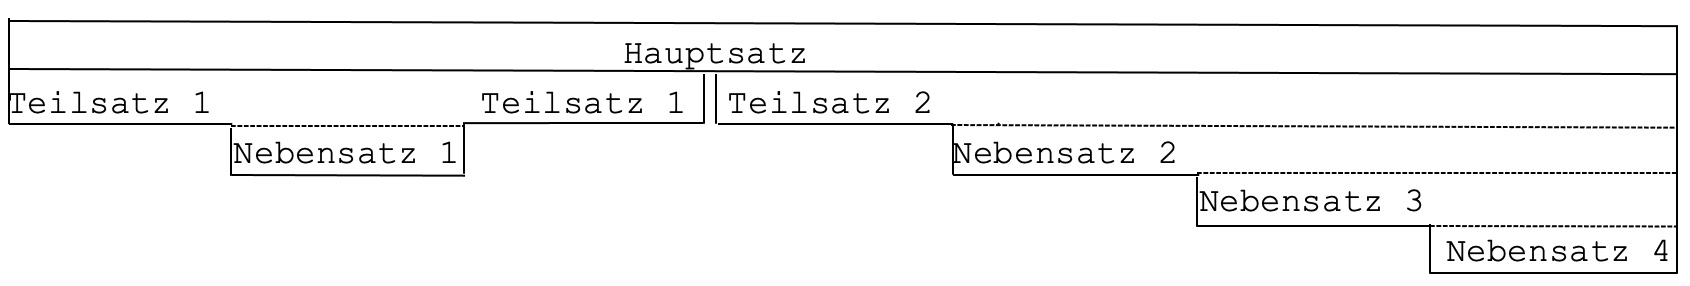
\includegraphics[width=12.5cm]{figures/Satzbild_Seghers}
    %% Abbildung 


\noindent\resizebox{\textwidth}{!}{
	
\begin{tabular}{ p{1.5cm} p{1.5cm} p{1.5cm} p{1.5cm} p{1.5cm} p{1.5cm} p{1.5cm} }
	
	\hline
	
	\multicolumn{7}{ | c | }{\hspace{2.5cm}\makecell[l]{\small\textcolor{gray}{Hauptsatz}}}  \\ \sbdashline{1-7} 
	
	\multicolumn{1}{ | l }{\makecell[l]{\small\textcolor{gray}{Teilsatz 1}}} &  
	\multicolumn{1}{l}{} & 	
	\multicolumn{1}{ l }{\makecell[l]{\small\textcolor{gray}{}}} &
	\multicolumn{4}{|| l | }{\makecell[l]{\small\textcolor{gray}{Teilsatz 2}}} \\ 
	\cline{1-1} \sbdashline{2-2} \cline{3-3}  \cline{4-4} \sbdashline{5-7}
	
	& \multicolumn{1}{ | l | }{\makecell[l]{\small\textcolor{gray}{Nebensatz 1}}} & & & 
	\multicolumn{3}{ | l | }{\makecell[l]{\small\textcolor{gray}{Nebensatz 2}}} \\ \cline{2-2} \cline{5-5} \sbdashline{6-7}
	
	& & & & & 
	\multicolumn{2}{ | l | }{\makecell[l]{\small\textcolor{gray}{Nebensatz 3}}} \\  \cline{6-6} \sbdashline{7-7}
	
	& & & & & &
	\multicolumn{1}{ | l | }{\makecell[l]{\small\textcolor{gray}{Nebensatz 4}}} \\  \cline{7-7}
	
	
\end{tabular}

}


	

    \caption{Satzbild zu (\ref{ea:Seghers_Satz})}
    \label{Abb:Satzbild_Seghrs}
\end{figure}


Der erste Nebensatz \textit{als ich krank und besinnungslos lag} ist ein Satzglied des ersten Teilsatzes. Es sättigt keine Valenzstelle des Hauptprädikats \textit{hatte gehofft}, sondern bestimmt den Zeitaspekt des Hauptsatzgeschehens und ist somit ein temporales Adverbial. Wir können den Nebensatz voranstellen (\ref{ea:Seghers_Satz_1_Nebensatz_Top}) und durch \textit{wann} ersetzen (\ref{ex:Seghers_Satz_1_Nebensatz_Frage}).

\ea \label{ea:Seghers_Satz_1_Nebensatz}
\ea \label{ea:Seghers_Satz_1_Nebensatz_Top} \textit{Als ich krank und besinnungslos lag}, hatte ich sogar manchmal auf jenen alten, frühen Namen gehofft.
\ex \label{ex:Seghers_Satz_1_Nebensatz_Frage} \textit{Wann} hatte ich sogar manchmal auf jenen alten, frühen Namen gehofft?
\z 
\z 

Die beiden Valenzstellen von \textit{hatte gehofft} werden durch \textit{ich} als Subjekt und \textit{auf jenen alten, frühen Namen} als Präpositionalobjekt gesättigt. Auch \textit{manchmal} ist ein Satzglied. Es drückt als temporales Adverbial aus, wie oft das Geschehen stattfand. 

Die Bestimmung von \textit{sogar} ist etwas komplizierter. Es drückt Erstaunen über etwas aus, hebt etwas als unerwartet hervor. Typischerweise fokussiert es als Attribut eine NP (\textit{sogar ich}/\textit{ich sogar}) oder eine PP (\textit{sogar auf jenen alten, frühen Namen}). Der Bezug wird durch die Stellung und die Betonung der fokussierten Größe deutlich. In dem Satz (\ref{ea:Seghers_Satz}) spricht die Stellung von \textit{sogar} jedoch für einen direkten Bezug auf das Hoffen-Szenario im Sinne von (\ref{ea:Seghers_Satz_sogar}).

\ea \label{ea:Seghers_Satz_sogar} Es war sogar so, dass ich manchmal, als ich krank und besinnungslos lag, auf jenen alten, frühen Namen hoffte.
\z 

Wir bestimmen \textit{sogar} als Kommentaradverbial (vgl. Abschnitt~\ref{subsection:Adverbial}). Die Schreiberin bewertet mit ihm das Hoffen-Szenario als etwas Erstaunliches, Besonderes. Für diese Bestimmung spricht die, wenn auch sehr markierte, alleinige Voranstellbarkeit von \textit{sogar} (\ref{ea:Seghers_Satz_sogar_Top}). 

\ea \label{ea:Seghers_Satz_sogar_Top} Sogar hoffte ich manchmal, als ich krank und besinnungslos lag, auf jenen alten, frühen Namen.
\z 

Hält man diese Stellung für unakzeptabel, dann wäre \textit{sogar} als Fokuspartikel ohne Satzgliedstatus zu bestimmen.

Innerhalb des Temporaladverbials \textit{als ich krank und besinnungslos lag} bildet \textit{lag} das Prädikat. Typischerweise verlangen sogenannte Positionsverben aufgrund ihrer Bedeutung nach einer Ergänzung in Form einer Lokalrelation wie \textit{im Bett liegen}. Analog kann jene Valenzstelle modal wie eben \textit{krank liegen} gesättigt werden. Bei anderen Verben würde es sich um ein Modaladverbial handeln. Da es sich hier um eine valenzielle Sättigung handelt, bestimmen wir \textit{krank und besinnungslos} als Modalergänzung.\footnote{Im Abschnitt~\ref{subsection:Adverbial} wurde jener zusätzliche Satzgliedtyp durch unseren valenziellen Ansatz begründet.}

Der nächste Teilsatz \textit{doch der Name blieb verloren} wird durch die Konjunktion \textit{doch} eingeleitet. Da sie weder Satzglied noch Attribut ist, wird sie in der Satzgliedanalyse nicht bestimmt. Das Prädikat \textit{blieb} verlangt als Kopulaverb nach einem Subjekt und nach einem Subjektsprädikativ (vgl. Abschnitt~\ref{subsection:SP und OP}). Diese Satzgliedfunktion übernimmt \textit{verloren}. Das Subjekt ist komplex, da die NP \textit{der Name} den appositiven Relativsatz mit weiteren eingebetteten Nebensätzen \textit{von dem ich in Selbsttäuschung glaubte, er könnte mich wieder gesund machen, jung, lustig, bereit zu dem alten Leben mit den alten Gefährten, das unwiederbringlich verloren war} als Attribut einbettet. Dass es sich bei dem ins Nachfeld ausgelagerten Komplex um einen Teil des Subjekts handelt, wird deutlich, wenn wir ihn zusammen mit seiner Bezugs-NP ins Vorfeld stellen (\ref{ea:Seghers_Satz_von_dem_Top}).

\ea \label{ea:Seghers_Satz_von_dem_Top} \textit{Doch der Name, von dem ich in Selbsttäuschung glaubte, er könnte mich wieder gesund machen, jung, lustig, bereit zu dem alten Leben mit den alten Gefährten, das unwiederbringlich verloren war,} blieb verloren.
\z 

Das Prädikat des Relativsatzes ist \textit{glaubte}. In der Bedeutung \gq{jemand meint in Bezug auf jemanden/etwas etwas} verlangt es nach drei Ergänzungen. Die erste Ergänzung \textit{ich} fungiert als Subjekt. Die PP \textit{von dem} ist Präpositionalobjekt. Der Inhalt des Glaubens wird durch den verkappten Nebensatz \textit{er könnte mich wieder gesund machen, jung, lustig, bereit zu dem alten Leben, mit den alten Gefährten, das unwiederbringlich verloren war} als Satzobjekt gesättigt. Dass dieser Komplex zusammen \textit{ein} Satzglied zum Prädikat \textit{glaubte} bildet, zeigt sich bei Pronominalisierung (\ref{ea:Seghers_Satz_glaubte_das}) sowie bei Voranstellung im umformulierten Hauptsatz (\ref{ex:Seghers_Satz_das_glaubte_HS}).

\ea \label{ea:Seghers_Satz_glaubte}
\ea \label{ea:Seghers_Satz_glaubte_das} Doch der Name, von dem ich \textit{das} in Selbsttäuschung glaubte, blieb verloren.
\ex \label{ex:Seghers_Satz_das_glaubte_HS} \textit{Er könnte mich wieder gesund machen, jung, lustig, bereit zu dem alten Leben, mit den alten Gefährten, das unwiederbringlich verloren war}, glaubte ich in Selbsttäuschung von dem Namen.
\z 
\z 

Die PP \textit{in Selbsttäuschung} ist ein Satzglied, das keine Valenzstelle sättigt. Es drückt eine Art und Weise des Glauben-Szenarios aus und ist somit ein modales Adverbial. Sinnvoll interpretieren wir es eher kausal als \gq{durch Selbsttäuschung}.

Das Satzobjekt zu \textit{glaubte} besteht intern wieder aus Satzgliedern. Sein Prädikat ist komplex und besteht aus dem Prädikat \textit{könnte machen} und den Objektsprädikativen \textit{wieder gesund}, \textit{jung}, \textit{lustig} und \textit{bereit}.\footnote{Auf \textit{wieder} gehen wir bei der Attributanalyse genauer ein.} Durch Koordination wird \textit{machen} als identischer Bestandteil jeweils ausgelassen. Da wir im Abschnitt~\ref{subsection:SP und OP} Objektsprädikative mikrovalenziell als Prädikatsteile bestimmt haben, stehen die Objektsprädikative \textit{jung}, \textit{lustig} und \textit{bereit} elliptisch für \textit{jung machen}, \textit{lustig machen} und \textit{bereit machen}. Wir analysieren sie daher getrennt als vier Objektsprädikative stellvertretend für koordinierte Prädikate. Als Subjekt fungiert \textit{er} und als Akkusativobjekt \textit{mich}. Durch das vierte Objektsprädikativ \textit{bereit} kommt es zu einer Valenzerhöhung. Die neue Valenzstelle wird durch die PP \textit{zu dem alten Leben mit den alten Gefährten, das unwiederbringlich verloren war} als Präpositionalobjekt gesättigt.   

Der appositive Relativsatz \textit{das unwiederbringlich verloren war} gehört zu \textit{dem alten Leben mit den alten Gefährten} und ist deshalb Teil des Präpositionalobjekts \textit{zu dem alten Leben mit den alten Gefährten, das unwiederbringlich verloren war}. Wird das Präpositionalobjekt wie in (\ref{ea:Seghers_Satz_dazu_bereit}) durch \textit{dazu} pronominalisiert, verschwindet auch der Relativsatz. Bei Voranstellung des Präpositionalobjekts im umformulierten Hauptsatz steht auch der Relativsatz als Satzgliedteil im Vorfeld (\ref{ex:Seghers_Satz_zu_dem_alten_Leben_HS}).

\ea \label{ea:Seghers_Satz_bereit_zu}
\ea \label{ea:Seghers_Satz_dazu_bereit} Doch der Name blieb verloren, von dem ich in Selbsttäuschung glaubte, er könnte mich wieder gesund machen, jung, lustig, \textit{dazu} bereit.
\ex \label{ex:Seghers_Satz_zu_dem_alten_Leben_HS} \textit{Zu dem alten Leben mit den alten Gefährten, das unwiederbringlich verloren war,} könnte er mich bereit machen.
\z 
\z 

Das Zentrum des Relativsatzes bildet die Kopulaform \textit{war} als Prädikat. Das den Relativsatz einleitende Demonstrativpronomen \textit{das} fungiert als Subjekt. Da es sich um ein Kopulaverb handelt, verlangt es nach einem Subjektsprädikativ. Diese Funktion erfüllt \textit{unwiederbringlich verloren}. Bei der Attributanalyse kommen wir auf die Beziehung zwischen \textit{unwiederbringlich} und \textit{verloren} zurück.   

Die Analyse wird in der Tabelle~\ref{tab:Seghers_Satz} gezeigt.

\begin{table}
%\tiny   
  \centering
  \resizebox{\textwidth}{!}{
  \begin{tabular}{l|l|l|l|l}
   % \lsptoprule
       &  Hauptsatz  &  1. NeSa-Ebene  & 2. NeSa-Ebene & 3. NeSa-Ebene \\
    \hline
    \textit{Ich} & Subjekt 1 & & & \\ \cline{2-2}
    \textit{hatte} & Prädikat 1 & & & \\ \cline{2-2} 
    \textit{sogar,} & Kommentaradverbial 1 & & & \\ \cline{2-2}
    \textit{als} & \multirow{6}{*}{Adverbial 1} & -- & & \\ \cline{3-3}
    \textit{ich} & & Subjekt & & \\ \cline{3-3}
    \textit{krank} & & \multirow{3}{*}{Modalergänzung} & & \\
    \textit{und} & & & & \\
    \textit{besinnungslos} & & & & \\ \cline{3-3}
    \textit{lag,} & & Prädikat & & \\ \cline{2-3}
    \textit{manchmal} & Adverbial 1 & & & \\ \cline{2-2}
    \textit{auf} & \multirow{5}{*}{Präpositionalobjekt 1} & & & \\ 
    \textit{jenen} & & & & \\ 
    \textit{alten} & & & & \\ 
    \textit{frühen} & & & & \\ 
    \textit{Namen} & & & & \\ \cline{2-2}
    \textit{gehofft,} & Prädikat 1 & & & \\ \cline{2-2}
    \textit{doch} & -- & & & \\ \cline{2-2}
    \textit{der} & \multirow{2}{*}{Subjekt 2} & & & \\ 
    \textit{Name} & & & & \\ \cline{2-2}
    \textit{blieb} & Prädikat 2 & & & \\ \cline{2-2} 
    \textit{verloren,} & Subjektsprädikativ 2 & & & \\ \cline{2-3}
    \textit{von} & \multirow{27}{*}{Subjekt 2} & \multirow{2}{*}{Präpositionalobjekt} & & \\ 
    \textit{dem} & & & & \\ \cline{3-3}
    \textit{ich} & & Subjekt & & \\ \cline{3-3}
    \textit{in} & & \multirow{2}{*}{Adverbial} & & \\ 
    \textit{Selbsttäuschung} & & & & \\ \cline{3-3}
    \textit{glaubte,} & & Prädikat & & \\ \cline{3-4}
    \textit{er} & & \multirow{21}{*}{Satzobjekt} & Subjekt & \\ \cline{4-4}
    \textit{könnte} & & & Prädikat & \\ \cline{4-4}
    \textit{mich} & & & Akkusativobjekt & \\ \cline{4-4}
    \textit{wieder} & & & \multirow{2}{*}{Objektsprädikativ 1} & \\ 
    \textit{gesund} & & & & \\ \cline{4-4}
    \textit{machen,} & & & Prädikat 1--4 \\ \cline{4-4}
    \textit{jung,} & & & Objektsprädikativ 2 & \\ \cline{4-4}
    \textit{lustig,} & & & Objektsprädikativ 3\\ \cline{4-4}
    \textit{bereit} & & & Objektsprädikativ 4 \\ \cline{4-4}
    \textit{zu} & & & \multirow{12}{*}{Präpositionalobjekt zu 4} & \\
    \textit{dem} & & & & \\
    \textit{alten} & & & & \\ 
    \textit{Leben} & & & & \\ 
    \textit{mit} & & & & \\ 
    \textit{den} & & & & \\
    \textit{alten} & & & & \\
    \textit{Gefährten,} & & & & \\ \cline{5-5}
    \textit{das} & & & & Subjekt \\ \cline{5-5}
    \textit{unwiederbringlich} & & & & \multirow{2}{*}{Subjektsprädikativ} \\
    \textit{verloren} & & & & \\ \cline{5-5}
    \textit{war.} & & & & Prädikat \\ 
    \hline 
   % \lspbottomrule
  \end{tabular}
  }
  \caption{Seghers-Satz}
  \label{tab:Seghers_Satz}
\end{table}

Kommen wir nun zu den Attributen innerhalb der ermittelten Satzglieder. Innerhalb des Präpositionalobjekts \textit{auf jenen alten, frühen Namen} beziehen sich \textit{alten} und \textit{frühen} als Adjektivattribute gleichrangig auf das Nomen \textit{Namen} als Bezugswort. Orthografisch wird die Gleichrangigkeit durch das Komma gekennzeichnet. 

Innerhalb der komplexen Subjekt-NP \textit{der Name, von dem ich in Selbsttäuschung glaubte, er könnte mich wieder gesund machen, jung, lustig, bereit zu dem alten Leben mit den alten Gefährten, das unwiederbringlich verloren war} bezieht sich der Relativsatz, zusammen mit den in ihn eingebetteten Nebensätzen, als Attribut appositiv auf \textit{der Name}. Allerdings folgt dieses komplexe Attribut nicht direkt seinem Bezugsausdruck, sondern steht, ausgeklammert, im Nachfeld.

Innerhalb des komplexen Objektsprädikativs \textit{wieder gesund} bezieht sich das Adverb \textit{wieder} attributiv auf sein Bezugsadjektiv \textit{gesund}. Diese Bestimmung ist durch die Lesart von \textit{wieder} motiviert. Hier geht es nicht um die Wiederholung des Geschehens \textit{gesund machen} im Sinne von \gq{noch einmal gesund machen}, sondern um die Wiederherstellung des Zustands \textit{gesund}.

Das Präpositionalobjekt \textit{zu dem alten Leben mit den alten Gefährten, das unwiederbringlich verloren war} ist durch verschiedene Attributbeziehungen komplex. Das Adjektiv \textit{alten} bezieht sich attributiv auf das Substantiv \textit{Leben} als Bezugswort. Die PP \textit{mit den alten Gefährten} bezieht sich ebenfalls als Attribut auf \textit{Leben}. Formal lässt sich keine Hierarchie zwischen den beiden Attributen ausmachen, also ob \textit{alten} Attribut zu \textit{Leben mit den alten Gefährten} ist oder ob \textit{mit den alten Gefährten} Attribut zu \textit{alten Leben} ist. Semantisch können wir die Eigenschaft \gq{alt} auf \textit{Leben mit den alten Gefährten} beziehen. Wir können aber auch \textit{mit den alten Gefährten} als eine Art näherer Bestimmung des \gq{alten Lebens} verstehen.

Innerhalb der attributiven PP \textit{mit den alten Gefährten} fungiert das Adjektiv \textit{alten} als Attribut zu \textit{Gefährten}. 

Der Relativsatz \textit{das unwiederbringlich verloren war} bezieht sich attributiv auf \textit{das alte Leben mit den alten Gefährten}. Hierfür spricht der appositive Charakter des Relativsatzes. Denn er dient nicht dazu, den Referenzbereich von \textit{Leben} einzugrenzen, sondern ist eine zusätzliche Information zu \textit{dem alten Leben mit den alten Gefährten}. Hierfür spricht die Möglichkeit, \textit{übrigens} einzufügen: \textit{das alte Leben mit den alten Gefährten, das übrigens unwiederbringlich verloren war}. 

Innerhalb des Subjektsprädikativs \textit{unwiederbringlich verloren}, bezieht sich das Adjektiv \textit{unwiederbringlich} attributiv auf \textit{verloren}. 

\chapter{Wort, Wortart und Flexion}\label{chapter:Wort}

Bisher haben wir uns mit den unmittelbaren Bausteinen des Satzes, den Satzkonstituenten (vgl. Kapitel~\ref{chap:Konstituenz}), und ihren Funktionen als Satzgliedern (vgl. Kapitel~\ref{chap:Satzgliedanalyse}) beschäftigt. Ebenso sind wir auf Bausteine innerhalb der Satzkonstituenten und auf ihre Funktion als Attribute (vgl. Abschnitt~\ref{section:SatzgliederundAttribute}) eingegangen. Den internen Bau der entsprechenden Wortgruppen haben wir unter dem Phrasenbegriff (vgl. Kapitel~\ref{chap:Phrasen}) dargestellt. 

Gehen wir auf die unterste Ebene, so gelangen wir zu den Wörtern bzw. zu konkreten Wortformen in konkreten Sätzen. Diese Wortformen werden auch syntaktische Wörter genannt. Sie bilden die mittelbaren Bestandteile von Sätzen und lassen sich aus unterschiedlichen Perspektiven als Wörter betrachten.

In dem folgenden Abschnitt~\ref{section:Wortbegriffe} stellen wir verschiedene Wortkonzepte vor. In Abschnitt~\ref{section:Wortarten} geht es um das Konstrukt von Wortarten. Diese werden dann in neun Unterkapiteln bezüglich ihrer Wortformenbildung, der Flexion und bezüglich ihrer Funktion dargestellt. Zuerst stellen wir in Abschnitt~\ref{section:Flektierbare} nacheinander die flektierbaren Wortarten vor. In Abschnitt~\ref{subsection:Verbflexion} geht es um Verben, in Abschnitt~\ref{subsection:Substantivflexion} um Substantive, in Abschnitt~\ref{subsection:Artikel_SGr_Flexion} um Artikel, in Abschnitt~\ref{subsection:Adjektiv_SGr_Flexion} um Adjektive und in Abschnitt~\ref{subsection:Pronomen_Flexion} um Pronomen. Danach beschäftigen wir uns in Abschnitt~\ref{section:Nicht flektierbar} mit wesentlichen Eigenschaften der nicht-flektierbaren Wortarten. In Abschnitt~\ref{subsection:Adverb} geht es um Adverbien, in Abschnitt~\ref{subsection:Präposition} um Präpositionen, in Abschnitt~\ref{subsection:Junktion} um Junktionen und in Abschnitt~\ref{subsection:Partikeln} um Partikeln. Der letzte Abschnitt~\ref{section:Aufgaben_Wort} bietet vier verschiedene Anwendungsaufgaben samt Lösungen zum Thema Wortart und Flexion. Vorab gehen wir aber in dem Exkurs~\ref{Exkurs:Wort_Schule} auf wesentliche Merkmale des vorschulischen Wortbegriffes ein und begründen, warum in der Schule ein formbasiertes Wortkonzept vermittelt werden sollte.


\begin{Exkurs}{Wortbegriff vor versus in der Schule}\label{Exkurs:Wort_Schule}

Als alphabetisierte Erwachsene erscheint uns der\is{Wortbegriff} Wortbegriff anders als syntaktische Funktionen als eine intuitive Größe. Gerade bei Vorschulkindern ist das aber nicht der Fall. \citet[110]{SteinigHuneke2015} zitieren die folgende Antwort einer Vierjährigen auf die Frage, was ein Wort sei: \gqq{Was man schreiben kann. Wörter.} und als Erklärung \gqq{A, I, U, Si, E}. Ein Siebenjähriger antwortete hingegen: \gqq{'n Wort issen langes Wort, zum Beispiel \textit{Die Eule sitzt aufm Baum}}. Die erste Antwort zielt auf geschriebene Wörter bzw. Buchstaben ab. Die zweite basiert eher auf dem Äußerungskonzept, auf welches auch der Begriff des \textit{Sprichwortes} abzielt. Wie \citet[55--56]{Bredel2013} schreibt, ist der vorschulische Wortbegriff eher bedeutungs-  und erfahrungsbezogen statt formbasiert.\footnote{\citet[52--57]{Bredel2013} bespricht auch verschiedene Experimente kritisch, die entsprechende Einsichten in den vorschulischen Wortbegriff erlaubt haben.} Ein Wort halten Vorschulkinder dann für lang, wenn das mit ihm bezeichnete Objekt groß ist. Schriftkundige Erwachsene ermessen die Wortlänge aus der Zahl der Buchstaben. Wortassoziationen sind bei Vorschulkindern eher szenisch, zu \textit{Tisch} assoziieren sie \textit{essen} und zu \textit{Bett} \zB \textit{ins Bett gehen}. Schriftkundigen hingegen fallen zu \textit{Tisch} eher andere Substantive, also Wörter derselben Wortart ein, die Möbel bezeichnen, also \zB \textit{Stuhl}, zu \textit{Bett} assoziieren sie eher  \textit{Sofa}. Wenn Vorschulkinder Wörter zählen sollen, halten sie sich eher an die Inhaltswörter, \zB an Substantive, die konkrete Dinge bezeichnen. Funktionswörter wie Artikel, Präpositionen und Hilfsverben fallen dabei erst einmal unter den Tisch. Das Wortverständnis von Vorschulkindern basiert primär auf ihrer Sprachfähigkeit, nicht aber auf Merkmalen von Formen.

Insbesondere in der Grundschule müssen wichtige Grundlagen für einen formbasierten Wortbegriff und damit auch für Sprachreflexion gelegt werden. Denn formbasierte Wortbegriffe spielen beim Erwerb der Schriftsprache eine wichtige Rolle. Wir müssen zwischen allen Wörtern Leerzeichen setzen. Aber was ist ein Wort? Substantive müssen wir großschreiben, auch dann, wenn sie nicht wie \textit{Sonne} etwas Dingliches bezeichnen, sondern \zB ein Geschehen wie \textit{das Schwimmen}. 

Wörter müssen in Wortgruppen betrachtet werden, da es um ihren Gebrauch als Instanz einer Wortart geht. So bemerkt \citet[12]{Granzow-Emden2006}, dass es sich bei \textit{Sonne} und \textit{schwimmen} zwar um typische Vertreter der Wortarten Substantiv und Verb handelt, nicht jedoch in der folgenden Äußerung: \textit{Nach dem Schwimmen sonne ich mich}. 

Um ein Substantiv korrekt gebrauchen zu können, müssen wir sein fixiertes Genus kennen. Und dieses hat primär nichts mit Geschlecht im alltäglichen Sinne zu tun: \textit{der Löffel}, \textit{das Messer}, \textit{die Gabel}. 

Substantive werden im Kasus dekliniert. Aber wo wird die entsprechende Markierung manifest? An manchem Eigenheim finden wir noch ein Schild mit der Aufschrift \textit{Warnung vor dem Hunde}, wir würden aber kaum sagen, ich habe Angst \textit{vor dem Hunde}. In der Schule haben viele \textit{Die Leiden des jungen Werther} gelesen, obwohl der Originaltitel von Goethe \textit{Die Leiden des jungen Werthers} heißt. 

Verben werden auch dann konjugiert, wenn es sich um Hilfs-, Modal-, Zustands- oder Vorgangsverben handelt. Also kann der Verbbegriff nicht an den bislang in der Schule gängigen Begriff des Tu-Wortes gebunden werden. 

Warum können wir sagen und schreiben \textit{eine häufige Erscheinung}, aber nicht *\textit{eine ofte Erscheinung}? Die Wörter \textit{häufig} und \textit{oft} haben zwar eine sehr ähnliche Bedeutung, aber sie gehören anderen Wortarten an. Das in seiner Wortform nach Genus, Kasus und Numerus veränderliche \textit{häufig} ist ein Adjektiv, das nicht veränderliche, aber satzgliedfähige \textit{oft} ist hingegen ein Adverb. 

In den folgenden Abschnitten dieses Kapitels werden wir zuerst verschiedene Wortbegriffe vorstellen und anschließend nach formalen Kriterien -- statt in der Schule gängiger pseudo-semantischer -- die Wortarten des Deutschen und ihre Eigenschaften beschreiben.          

\end{Exkurs}


\section{Wortbegriffe}\label{section:Wortbegriffe}

Zwar sprechen wir alltäglich einfach von einem Wort, \zB wenn wir sagen, dieses Wort stehe nicht im Wörterbuch oder wenn wir fragen, was dieses oder jenes Wort bedeute. Aber schon die beiden Pluralformen \textit{Wörter} und \textit{Worte} zielen auf unterschiedliche Wortkonzepte ab. Im Folgenden werden wir anstelle einer allumfassenden Wortdefinition verschiedene Wortbegriffe skizzieren: graphematische Wörter, d.\,h. Buchstabenketten ohne Leerzeichen, Wörter als kleinste syntaktisch selbstständige Einheiten aus Form und Bedeutung, d.\,h. als Zeichen. Was die Bedeutung angeht, werden wir zwischen Inhalts- und Dienstwörtern unterscheiden, die jeweils eine offene und eine geschlossene Klasse bilden. Für abstrakte Grundeinheiten aus Form und Bedeutung führen wir den Lexembegriff ein, für die formale Anpassung eines Lexems an eine bestimmte syntaktische Umgebung den Flexionsbegriff. Als Wortstamm werden wir reale Formen ohne Flexion bezeichnen.\footnote{Eine Übersicht und Diskussion der Wortkriterien bietet \citet[30--35]{Wurzel2000}.}

Wörter sind minimal selbständige, d.\,h. als syntaktische Grundbausteine verwendbare bedeutungstragende Einheiten wie \zB \textit{Tag} oder \textit{auf}. Sie bestehen formal aus einer Lautkette {[taːk]} bzw. {[a\textupsilon f]} (vgl. Kapitel \ref{kap:Phonetik}) mit einer einheitlichen Akzentstruktur, die sie meistens von Wortgruppen unterscheidet: (\textit{das}) \textit{Tageslicht} mit Betonung auf \textit{Tag} versus (\textit{des}) \textit{Tages Licht} mit Betonung auf \textit{Licht}. Schriftlich bestehen sie aus einer Kette von Buchstaben bzw. genauer gesagt von Graphemen (vgl. Kapitel \ref{kap:Graphematik}). Mit der Form ist eine Bedeutung assoziiert.

Insbesondere die\is{Wortbegriff!graphematisch} durch Leerzeichen abgegrenzte Graphemkette bildet die Grundlage für das in der Schule zentrale Konzept des \textit{graphematischen Wortes}. So besteht (\ref{ea:5Wörter}) aus fünf graphematischen Wörtern, (\ref{ex:4Wörter}) hingegen aus vier graphematischen Wörtern. Für (\ref{ex:zuhause}) gilt sowohl die Einwortschreibung als auch die empfohlene Zweiwortschreibung als richtig.

\ea \label{ea:graph_Wort}
\ea \label{ea:5Wörter} denn wir kommen heute an
\ex \label{ex:4Wörter} weil wir heute ankommen
\ex \label{ex:zuhause} zuhause, zu Hause 
\z 
\z 

Die\is{Wortbegriff!Form-Bedeutung} Verbindung zwischen Form und Bedeutung ergibt ein Zeichen. Es beruht auf historisch gewachsenen Konventionen innerhalb einer Sprachgemeinschaft. Bedeutungen, wie wir sie in Wörterbüchern finden, sind Abstraktionen aus den Gebrauchskontexten. So lassen sich bei \textit{Tag} zwei Bedeutungen formulieren: \gq{Zeit zwischen Morgen- und Abenddämmerung} oder aber \gq{24 Stunden von Mitternacht bis Mitternacht}. Erstere ist die ursprüngliche Bedeutung, welche der Bedeutung von \textit{Nacht} gegenübersteht.\footnote{Hierfür spricht die Herkunft des Wortes \textit{Tag} aus einer indoeuropäischen Wurzel, die so viel wie \gq{brennen} bedeutet als \gq{Zeit, in der die Sonne brennt}. Hierauf gehen Redewendungen wie \textit{an den Tag kommen} zurück. Cf. \citet[541]{Paul1908Woerterbuch}.} Letztere ist eine begriffliche Definition, welche sich aus dem Rhythmus von Vergehen und Wiederkehr der hellen Zeit ergibt, aber die Nacht einschließt.

Die ursprünglich lokale Bedeutung von \textit{auf} lässt sich beschreiben als \gq{Position an der Oberfläche eines Gegenstandes} (\textit{der Mann auf dem Mond}) oder als \gq{Richtung zu einer Oberfläche hin} (\textit{der Flug auf den Mond}).

Nehmen wir\is{Wortbegriff!Listem} die Bedeutungsseite zum Ausgangspunkt der Wortbestimmung, dann können auch mehrere orthografische Wörter ein Zeichen bilden wie \zB \textit{Rote Beete} oder die Süßspeise \textit{Crème brûlée}. Lässt sich die Gesamtbedeutung eines Ausdrucks nicht aus den einzelnen Wörtern und ihrer Verbindung ermitteln, so handelt es sich auch bei idiomatisch fixierten Ausdrücken wie in (\ref{ea:Idiom1}) und (\ref{ex:Idiom2}) um jeweils ein komplexes Zeichen oder \textit{Listem}, also um eine im mentalen Lexikon holistisch gespeicherte (gelistete) Einheit. 

Aus didaktischer Sicht sollten zu den Listemen auch sogenannte Kollokationen\footnote{Unter \textit{Kollokationen} werden besonders häufige und besonders typische Verbindungen von Wörtern verstanden. Neben \textit{die Zähne putzen} (statt \textit{waschen} oder \textit{bürsten}) \zB \textit{eine Reise buchen}, \textit{harte} vs. \textit{weiche Drogen} oder \textit{ein Wort nachschlagen}.} wie in (\ref{ex:Kollokation}), Nominalisierungs- (\ref{ex:NVGListem}) sowie Funktionsverbgefüge (\ref{ex:FVGListem}) gezählt werden (vgl. Abschnitt~\ref{subsection:IdiomeNVGFVG}).

\ea \label{ea:Listeme}
\ea \label{ea:Idiom1} Wes Brot ich ess, des Lied ich sing.
\ex \label{ex:Idiom2} den Nagel auf den Kopf treffen
\ex \label{ex:Kollokation} die Zähne putzen 
\ex \label{ex:NVGListem} einen Besuch abstatten
\ex \label{ex:FVGListem} zur Aufführung bringen
\z 
\z 

Ferdinand de \citet[158--160]{SaussureCLG72} hat in seinem 1916 erstmals postum veröffentlichten \textit{Cours de linguistique générale} den Begriff des\is{Zeichenwert} \textit{Zeichenwertes} geprägt. Der Wert eines Zeichens ergibt sich sprachspezifisch aus der Differenz zu anderen verwandten Zeichen. Bei \textit{Tag} wären das \zB \textit{Nacht} und \textit{Dämmerung} sowie \textit{Stunde} und \textit{Woche}. Der Differenzwert wird insbesondere bei abstrakteren Wörtern wie bei Präpositionen interessant. So ergibt sich der Wert von \textit{auf} durch die Differenz zu den Präpositionen \textit{an}, \textit{über} und \textit{in}. Auch beim Sprachvergleich kommt der Wertbegriff zum Tragen. So wird \zB der Wert des deutschen Wortes \textit{Himmel} im Englischen auf zwei Zeichen aufgeteilt: \textit{sky} für den \gq{Himmel als Firmament} und \textit{heaven} für das \gq{göttliche Himmelreich}. 

Bedeutung ist immer sprachliche Bedeutung, die sich aus dem Zeichenwert ergibt und als Merkmalsbündel beschreibbar ist. Im Abschnitt~\ref{subsection:Verbklassen} haben wir diese sprachliche Bedeutung als\is{Signifikat} \textit{Signifikat} bezeichnet. Erst das Signifikat ermöglicht es, mit Wörtern in Sätzen auf außersprachliche Dinge und Beziehungen zu verweisen (Referenz). Das in der Welt Bezeichnete wird\is{Denotat} \textit{Denotat} genannt. Den Unterschied zwischen Signifikat (Sprache) und Denotat (Welt) hat der Logiker \citet[27]{Frege1892} am Beispiel von \textit{Morgenstern} und \textit{Abendstern} deutlich gemacht. Beide bezeichnen denselben Planeten, nämlich die Venus. Die sprachliche Bedeutung perspektiviert aber unterschiedliche Merkmale, nämlich einmal das Erscheinen vor der Sonne am Morgen und das andere Mal das frühe Erscheinen am Abendhimmel.\footnote{Bei \citet{Frege1892} sind die Begrifflichkeiten anders: die Bezeichnung in der Welt ist bei Frege die \textit{Bedeutung} und die sprachliche Vorstellung der \textit{Sinn}. Heute wird auch von \textit{Extension} und \textit{Intension} gesprochen.}

Bezüglich der\is{Wortklasse!Inhaltswort} Bedeutung\is{Wortklasse!Dienstwort} unterscheiden wir zwischen Wörtern, die wie das Substantiv \textit{Tag}, das Adjektiv \textit{hell}, das Verb \textit{arbeiten} oder das Adverb \textit{morgen} unmittelbare Vorstellungen evozieren und solchen wie der Subjunktion \textit{dass}, dem bestimmten Artikel \textit{der} und dem Pronomen \textit{dieser}. Letztere dienen der grammatischen Organisation von Wortgruppen und Sätzen sowie der Orientierung des Hörers in Texten und im Gespräch. \citet[63--70]{Tesniere1980deutsch} bezeichnet die ersteren bezüglich ihres Inhalts als \textit{volle} und die letzteren als \textit{leere Wörter}. Wir können auch von \textit{Inhaltswörtern} oder \textit{Autosemantika} (selbstbedeutenden Wörtern) und mit \citet[43]{Erben1980} von \textit{Dienstwörtern} oder \textit{Synsemantika} (semantisch unselbständigen Wörtern) sprechen. Die Grenzen verlaufen allerdings durch die traditionellen Wortarten. So zählt die Subjunktion \textit{dass} sicher zu den Dienstwörtern, die Subjunktion \textit{nachdem} hat hingegen eine klare lexikalische Bedeutung. Der Prototyp des Wortbegriffs zielt auf die Inhaltswörter ab.

Mit \citet[37]{Eisenberg2020_Wort} können\is{Wortklasse!offen} die Inhaltswörter auch als \textit{offene} und die\is{Wortklasse!offen} Dienstwörter als \textit{geschlossene} Klasse bezeichnet werden. Denn der Bestand der Inhaltswörter kann \zB durch Entlehnung aus anderen Sprachen wie \textit{Home Office} oder durch Neubildungen wie \textit{Heimbüro} beständig anwachsen. Darauf zielt der Begriff der \textit{offenen} Klasse ab. Bei den Dienstwörtern ist das nicht der Fall. Ihr Bestand ist über lange Zeiträume viel stabiler, weshalb sie eine \textit{geschlossene} Klasse bilden.

Denken wir\is{Lemma} an Einträge in einem Wörterbuch, so steht ein Stichwort, das \textit{Lemma}, stellvertretend, quasi wie ein Familienname an der Klingel, für verschiedene Wortformen. So steht \textit{Tag} nicht nur für \textit{Tag} selbst, sondern auch für \textit{Tage} in (\ref{ea:Tage1}) und (\ref{ex:Tage2}), für \textit{Tages} in (\ref{ex:Tages}) und für \textit{Tagen} in (\ref{ex:Tagen}).
 
\ea \label{ea:LemmaTag}
\ea \label{ea:Tage1} am \textit{Tage} seiner Geburt
\ex \label{ex:Tage2} die \textit{Tage} vergehen
\ex \label{ex:Tages} der Höhepunkt des \textit{Tages}
\ex \label{ex:Tagen} an warmen \textit{Tagen}
\z 
\z 

Abstrahieren wir\is{Lexem} von einer konkreten formalen Realisierung, von einem konkreten Exemplar oder einem Vorkommnis, so sprechen wir von einem \textit{Lexem} als dahinterstehendem Typ. Die konkreten Exemplare \textit{Tage}, \textit{Tage}, \textit{Tages}, \textit{Tagen} in (\ref{ea:LemmaTag}) sind Instanzen \textit{eines} abstrakten Lexems.     

\begin{Definition}{Lexem}\label{Def:Lexem}
    
\noindent Ein Lexem ist eine virtuelle Einheit aus Form und Bedeutung. Seine Formseite wird durch ein Laut- und/oder Schriftbild repräsentiert. Lexeme lassen sich Wortarten zuordnen. Je nach Zugehörigkeit zu einer Wortart kann ein Lexem über verschiedene (flektierte) Formen verfügen.  
\end{Definition}



Die Wortformen entstehen durch\is{Flexion} \textit{Flexion} (lat. \gq{Biegung} oder \gq{Beugung}). Flexion bezeichnet die Änderung der Wortform, die typischerweise durch Endungen, die Flexionsaffixe, realisiert wird. Die so gebildeten Wortformen dienen dem Ausdruck bestimmter grammatischer Merkmale wie Dativ Singular in (\ref{ea:Tage1}), Nominativ Plural in (\ref{ex:Tage2}), Genitiv Singular in (\ref{ex:Tages}) oder Dativ Plural in (\ref{ex:Tagen}). Hier handelt es sich um \textit{syntaktische Wörter}, die für eine ganz bestimmte Funktion in einer ganz bestimmten Wortgruppe kategorisiert sind. \citet[7]{Boettcher2009Wort} bezeichnet sie metaphorisch als \gqq{grammatische Aufrüstungen} eines Lexems.


\begin{Definition}{Flexion und Flexionsparadigma}
    
\noindent Flexion ist die Bildung von Wortformen eines Lexems. Die Gesamtheit der Wortformen eines Lexems bildet dessen Paradigma. Flexion dient der grammatischen Anpassung eines Lexems an seine syntaktische Funktion in einer Wortgruppe. Die Wortformenbildung erfolgt nach verschiedenen Flexionskategorien. Sie wird durch Flexive, sowie durch Stammveränderungen wie Umlaut und Ablaut und durch Hilfswörter realisiert. 
\end{Definition}


Die verschiedenen Flexionsformen sind Abwandlungen des\is{Wortstamm} \textit{Wortstamms}. So handelt es sich bei \textit{Tages}, \textit{Tage} und \textit{Tagen} um Abwandlungen des Wortstamms \textit{Tag}, der ohne formale Auszeichnung gleichzeitig eine Wortform ist. Ein Lexem kann über verschiedene Wortstämme oder Stammformen verfügen. Ein starkes Verb wie \textit{fahren} zum Beispiel weist die Stammformen \textit{fahr-} und \textit{fuhr-} auf. Auch Substantive, deren Pluralform mit einem Umlaut gebildet wird, verfügen über verschiedene Stammformen, so \zB \textit{Haus} über die Stammform \textit{Haus-} für die Flexionsformen \textit{Haus}, \textit{Hause}, \textit{Hauses} und über \textit{Häus-} für die Flexionsformen \textit{Häuser} und \textit{Häusern}. 

\begin{Definition}{Wortstamm}\label{def:Wortstamm}
    
\noindent 
Ein Wortstamm ist der lexikalische (bedeutungstragende) Grundbaustein eines Wortes, an den Flexionsaffixe angehängt werden können. Folglich ist der Wortstamm eine Wortform minus Flexionsaffix. Lexeme können über verschiedene Stämme verfügen.  
\end{Definition}


Lexeme können\is{Nennform (Wort)} wir nicht direkt nennen, da sie virtuell sind. In Wörterbüchern verwenden wir sogenannte \textit{Nennformen} oder \textit{Lemmata}. Im Deutschen entsprechen die Nennformen von Substantiven weitgehend den Stämmen, die wiederum mit der Wortform für den Nominativ Singular identisch sind. So ist \zB \textit{Haus} sowohl der Stamm als auch die Nennform und die Form für den Nominativ Singular. Bei Adjektiven entsprechen der Stamm und die Nennform der flexionslosen Kurzform. So ist \zB \textit{grün} die Nennform und der Stamm, der zu den Wortformen \textit{grüner}, \textit{grünes}, \textit{grüne}, \textit{grünen}, \textit{grünem} abgewandelt werden kann. Bei Verben weicht die Nennform, der Infinitiv, grundsätzlich vom Stamm ab. Denn Infinitive verfügen über das Flexionsaffix \textit{-en}. So ist \zB \textit{machen} die Nennform, aber \textit{mach-} ist der Stamm.  

Alle durch Flexion von einem Stamm ableitbaren Wortformen bilden ein\is{Wortparadigma} \textit{Wortparadigma}. Das Paradigma von \textit{Tag} besteht aus \textit{Tag}, \textit{Tage}, \textit{Tages} und \textit{Tagen}. Andere Wörter wie \textit{dass} oder \textit{dort} sind nicht flektierbar. Deshalb bilden sie kein Paradigma bzw. das Paradigma besteht aus genau einer unflektierbaren Form. 

Im Alltag werden wir uns der Flexion eigentlich nur bewusst, wenn Unsicherheiten auftreten. Heißt es \textit{die Denkmale} oder \textit{die Denkmäler}? Kann man schreiben \textit{ich bügel} oder \textit{bügele} oder \textit{bügle}? Hat jemand den \textit{Präsident} oder den \textit{Präsidenten} getroffen? 

Flektierbarkeit und Flexion sind ein wesentliches Kriterium bei der Abstraktion von Wortarten aus einzelnen Wörtern. Hierum geht es in dem folgenden Abschnitt~\ref{section:Wortarten}.
 
 
\section{Wortartenkonzepte}\label{section:Wortarten}

Die älteste\is{Wortart!Kanon} grammatische und insbesondere\is{Schulgrammatik} schulgrammatische Tradition hat die Zuordnung von Wörtern zu Wortarten.\footnote{Besonders prominent ist die Klassifizierung der Wortarten in der griechischen Grammatik von Dionysios Thrax aus dem ersten Jahrhundert v.\,Chr. Thrax unterscheidet acht Wortarten: Nomen, Verb, Partizip, Artikel, Pronomen, Präposition, Adverb und Konjunktion. Seit \citet[278]{Adelung1782} wird das Partizip zwar noch unter den Wortarten aufgezählt, aber bei attributiver Verwendung nach heutigem Verständnis dem Adjektiv zugeordnet.} So bestimmen wir \textit{Tag} als Substantiv, \textit{täglich} als Adjektiv und \textit{tagen} als Verb. Seit \citet[71--79]{Adelung1782} bilden die folgenden zehn Wortarten einen relativ stabilen Kanon in der deutschen Schulgrammatik: Substantiv (Hauptwort), Artikel, Zahlwort (Numerale), Adjektiv, Pronomen, Verb, Adverb, Präposition, Konjunktion, Interjektion. Das aktuelle \citet[13--17]{KMK2019} behält diesen Kanon mit einigen Modifikationen bei.\footnote{Neben dem Adverb werden Kommentaradverbien wie \textit{leider} und Konjunktionaladverbien wie \textit{deshalb} unterschieden. Das Zahlwort (Numerale) wird nicht als eigene Wortart bestimmt, sondern den Adjektiven zugerechnet. Stattdessen werden \textit{Partikeln} wie \textit{denn} in \textit{Was machst du denn?} als Wortart aufgeführt.}

Die Klassifizierung\is{Wortart!Kriterien} beruht seit jeher auf drei verschiedenen Kriterien: auf semantischen, auf morphologischen und auf syntaktischen. So wurden \zB die Numeralia wie \textit{zwei} oder \textit{zweite} semantisch als Zahlwort bestimmt. Mitunter werden in der Grundschule das Substantiv primär als Ding- und das Verb als Tu-Wort bestimmt. 

Bei dem morphologischen Kriterium geht es primär um Flexion. Wortarten werden danach bestimmt, nach welchen Kategorisierungen ihre Form verändert (flektiert) wird. Verben werden nach Person, Numerus, Tempus usw. konjugiert. Hingegen werden Substantive in Abhängigkeit von ihrem festgelegten Genus nach Numerus und Kasus dekliniert. Bei den Adjektiven, Pronomen und Artikeln kommt noch das Genus als flexible Kategorisierung hinzu. Adjektive können anders als Pronomen und Artikel auch gesteigert (kompariert) werden. Allerdings handelt es sich hierbei nicht um eine Kategorisierung der Flexion, sondern der Wortbildung. Bezüglich der Flexion ist das Alleinstellungsmerkmal von Adjektiven, dass sie je nach Umgebung schwach und stark flektieren: \textit{der frisch-e Fisch} versus \textit{frisch-er Fisch}.     

Wörter, die nicht flektierbar sind wie \zB \textit{dass}, \textit{dort} und \textit{auf} werden nach syntaktischen Eigenschaften bestimmt. So leitet die Subjunktion \textit{dass} Nebensätze mit Verbendstellung ein. Das Adverb \textit{dort} ist satzglied- und damit vorfeldfähig. Die Präposition \textit{auf} regiert eine NP im Dativ oder im Akkusativ. 

Dieses Kriteriengemisch wurde schon durch \citet[96]{Suetterlin1907} als \gqq{(wissenschaftlich) nicht haltbar} kritisiert. Idealerweise sollte ein einziges Kriterium der Klassifizierung dienen. Prominent ist der Vorschlag von \citet[53]{Glinz1962}, die Wortarten strikt nach dem morphologischen Kriterium (Formveränderlichkeit) zu bestimmen. 

Das ergibt fünf Wortarten, nämlich die drei flektierbaren, offenen Inhaltswortarten Substantiv, Verb und Adjektiv. Dazu kommt die geschlossene Klasse der Pronomen, einschließlich der Artikel, als Dienstwörter. Diesen vier Wortarten stehen alle anderen Wörter, da unflektierbar, als \textit{Partikeln} gegenüber. Allerdings beginnt dann doch wieder eine feinere Differenzierung der Partikeln in die drei syntaktischen Funktionsklassen Adverb, Präposition und Konjunktion. Das Ergebnis der Glinz'schen Einteilung weicht im Endeffekt nicht wesentlich von der traditionellen Einteilung ab. Es legt das jeweils angewandte Kriterium in zwei Schritten offen. Diese Einteilung wird im Wesentlichen von der \citet[§1005, 594]{Duden2022} übernommen.

Auch \citet[19]{HelbigBuscha}, die anders als \citet{Glinz1962}, primär das syntaktische Kriterium anwenden, unterscheiden zwischen neun Wortarten. Zwar zählen sie Pronomen zu den Substantivwörtern, weil sie anstelle einer Substantivgruppe stehen können. Aber auch sie arbeiten mit dem Begriff des Pronomens. Anstelle einer gemeinsamen Klasse der Konjunktionen unterscheiden \citet[20]{HelbigBuscha} zwischen den unterordnenden Subjunktionen und den nebenordnenden Konjunktionen. 

Praktisch gehen\is{Distributionstest} \citet[19--20]{HelbigBuscha} so vor, dass sie ein zu bestimmendes Wort innerhalb einer gegebenen syntaktischen Struktur (Distribution) löschen und durch andere Wörter ersetzen (Substitution). Wörter, die die gleiche Stelle im Satz einnehmen können, werden einer syntaktischen Wortklasse zugeordnet. Soll \zB die Wortklasse von \textit{Blau} in (\ref{ea:Wortklasse_Blau}) bestimmt werden, so wird es in der gegebenen Umgebung gelöscht (\ref{ex:Wortklasse_Löschen}), was wir durch eine leere Box symbolisieren. Nun wird geprüft, welche Wörter die Stelle von \textit{Blau} in der Box in (\ref{ex:Wortklasse_Löschen}) einnehmen könnten. Wir könnten \zB \textit{Grün}, \textit{Tal}, \textit{Schnurren} einsetzen, aber nicht \textit{schnurrt}.  

\ea \label{ea:syntaktische Wortklassen}
\ea \label{ea:Wortklasse_Blau} Dieses tiefe Blau gefällt mir.
\ex \label{ex:Wortklasse_Löschen} Dieses tiefe \fbox{\phantom{Blau}} gefällt mir.
\z 
\z 

Ausgehend von einem prototypischen Substantiv wie \textit{Tal} können \textit{Blau}, \textit{Grün} und \textit{Schnurren} innerhalb der Distribution von (\ref{ex:Wortklasse_Löschen}) als Mitglieder einer syntaktischen Klasse bestimmt werden. Es handelt sich um Köpfe einer NP (vgl. Abschnitt~\ref{section:NP}), was ihre Großschreibung bedingt. Insofern kann der Test praktisch gerade dann sinnvoll sein, wenn wie bei \textit{Blau}, \textit{Grün} und \textit{Schnurren} ein Wortartenwechsel vorliegt, um den es im Abschnitt~\ref{subsection:Konversion} geht. 

Der Test in (\ref{ea:syntaktische Wortklassen}) für sich klärt noch nicht, warum wir \textit{Blau}, \textit{Grün}, \textit{Tal} und \textit{Schnurren} in (\ref{ex:Wortklasse_Löschen}) als Substantive gebrauchen. Hierfür müssen die Formmerkmale, die das Vorkommen in der Umgebung (\ref{ex:Wortklasse_Löschen}) bedingen, beschrieben werden. Substantiv zu sein, genügt nicht, um in (\ref{ex:Wortklasse_Löschen}) akzeptabel zu sein: \textit{Täler} oder \textit{Grünes} können wir nicht einsetzen. 

Ebenfalls ist durch die Distributionsprobe nicht zu klären, warum \textit{blau} und \textit{grün} für sich genommen primär als Adjektiv klassifiziert werden und \textit{schnurren} als verbaler Infinitiv, was nichts an ihrem Status als Kopf der NP (und dem damit verbundenen temporären Substantivstatus) in (\ref{ex:Wortklasse_Löschen}) ändert. 

Trotz aller Unterschiede hat sich ein Kanon von Kategorien etabliert -- sei es als Wortarten oder Unterwortarten -- um formale und funktionale Gemeinsamkeiten von Wörtern in Sätzen oder Wortgruppen zu erfassen. Der Wortbestand lässt sich nicht hinreichend durch ein einziges Kriterium untergliedern. Somit sollte nicht die Anwendung mehrerer Kriterien kritisiert werden, sondern die invariante, anhand eines Merkmals vorzunehmende Kategorisierungsmethode.

Wesentlich ist\is{Wortart!Kriterien} das Verständnis, dass es sich bei Wortarten um Klassen handelt, die nach verschiedenen Kriterien von Menschen etabliert werden. Anders als in der Schule suggeriert wird, sind Wortarten keine Gegebenheiten der Sprache an sich.\footnote{Cf. \citet[99]{Gehrig2014}.} Wer sich mit Wortarten beschäftigt, konstruiert diese nach bestimmten Kriterien. Und wer Klassen in einer natürlichen Sprache bildet, der muss akzeptieren, dass nicht alle Wörter widerspruchslos und vollständig über \textit{ein} gemeinsames Merkmal nur \textit{einer} Klasse zuzuordnen sind.\footnote{Cf. \citet[4--6]{Lehmann2005Wortart}.}

Im\is{Wortart!Übersicht} Folgenden werden die Wortarten nach zwei Kriterien bestimmt. Die erste Unterteilung ist morphologisch motiviert in Wortarten, die flektierbar [+flektierbar] und solche, die nicht flektierbar [-flektierbar] sind. Flektierbar sind Verben, Substantive, Adjektive, Pronomen und Artikel. Um ihre Flexion und ihre Charakterisierung geht es in dem Unterkapitel \ref{section:Flektierbare}. 

Danach werden die nicht flektierbaren nach syntaktischen Kriterien im Unterkapitel \ref{section:Nicht flektierbar} differenziert: das Adverb als satzgliedfähige Wortart, die Präposition als kasusregierende Wortart, die Junktion als verknüpfende Wortart mit der Konjunktion für Nebenordnung, mit der Subjunktion für Unterordnung und mit der Adjunktion zum Anschluss von Vergleichswerten. Die Partikel wird negativ als ein Sammelsurium bestimmt. Negativ bestimmtes Sammelsurium deshalb, weil sie zwar Eigenschaften haben, welche die übrigen nicht flektierbaren Wortarten nicht aufweisen, ansonsten aber sehr heterogen sind. Es handelt sich zumeist um Herausentwicklungen aus der Gruppe der Adverbien und der Junktionen.

Eine Übersicht wird in der Abbildung \ref{caption:Wortarten} dargestellt.

\begin{sidewaysfigure}
	 %\resizebox{0.98\textwidth}{!}{
		%\begin{minipage}{\textwidth}
	%\centering
     \fittable{
	\begin{forest}
		 %/tikz/every node/.append style={font=\footnotesize},
		%for tree={l sep=2em, s sep=2.5em},
		[Wortarten [+flektierbar [konjugierbar\\Tempus [\textbf{Verb}\\\textit{gibst, gab,} \\\textit{gegeben}]] [deklinierbar\\Kasus\\\textbf{Nomen} [festes Genus [\textbf{Substantiv}\\\textit{Buch, Buches}\\\textit{Bücher}
		]] [variables Genus [2 Flexionsklassen [\textbf{Adjektiv}\\\ (\textit{das}) \textit{kleine} (\textit{Kind})\\ (\textit{ein}) \textit{kleines} (\textit{Kind})]][1 Flexionsklasse [im Status einer NP\\\textbf{Pronomen}\\\textit{sie, ihr}] [Teil einer NP\\\textbf{Artikel}\\\textit{der, den}] ]]] ] [--flektierbar [+satzgliedfähig [\textbf{Adverb}\\\textit{gerne}]] [--satzgliedfähig [+kasus-\\regierend [\textbf{Präposition}\\\textit{auf}] ] [--kasus-\\regierend [+verknüpfend [\textbf{Junktion} [+unterordnend [\textbf{Subjunktion}\\\textit{dass} ]] [--unterordnend [+reihend [\textbf{Konjunktion}\\\textit{und}] ] [--reihend [\textbf{Adjunktion}\\\textit{als, wie}] ] ]  ]  ] [--verknüpfend [\textbf{Partikel}\\\textit{sehr}] ] ] ] ]]
	\end{forest}
	\caption{Wortarten und Unterarten}\label{caption:Wortarten}

%\end{minipage}
}
\end{sidewaysfigure}

% \noindent
% \oneline{
% 	\begin{forest}
% [Wortarten
%   [+flektierbar
%     [konjugierbar\\Tempus
%       [\textbf{Verb}\\\textit{gibst, gab,} \\\textit{gegeben}]
%     ]
%     [deklinierbar\\Kasus
%       [\textbf{Nomen}
%         [festes Genus,tier=genus
%           [\textbf{Substantiv}\\\textit{Buch, Buches}\\\textit{Bücher}]
%         ]
%         [variables Genus,tier=genus
%           [2 Flexionsklassen
%             [\textbf{Adjektiv}\\\ (\textit{das}) \textit{kleine} (\textit{Kind})\\ (\textit{ein}) \textit{kleines} (\textit{Kind})]
%           ]
%           [1 Flexionsklasse
%             [im Status einer NP\\\textbf{Pronomen}\\\textit{sie, ihr}]
%             [Teil einer NP\\\textbf{Artikel}\\\textit{der, den}
%             ]
%           ]
%         ]
%       ]
%     ]
%   ]
%   [--flektierbar
%     [--satzgliedfähig
%       [+kasus-\\regierend
%         [\textbf{Präposition}\\\textit{auf}]
%       ]
%       [--kasus-\\regierend
%         [+verknüpfend
%           [\textbf{Junktion}
%             [+unterordnend
%               [\textbf{Subjunktion}\\\textit{dass} ]
%             ]
%             [--unterordnend
%               [+reihend
%                 [\textbf{Konjunktion}\\\textit{und},tier=genus]
%               ]
%               [--reihend
%                 [\textbf{Adjunktion}\\\textit{als, wie}]
%               ]
%             ]
%           ]
%         ]
%         [--verknüpfend
%           [\textbf{Partikel}\\\textit{sehr}]
%         ]
%       ]
%     ]
%     [+satzgliedfähig
%       [\textbf{Adverb}\\\textit{gerne}]
%     ]
%   ]
% ]
% 	\end{forest}
% }


\section{Flektierbare Wortarten}\label{section:Flektierbare}

In den folgenden Abschnitten stellen wir die flektierbaren Wortarten vor. Flektierbare Wortarten zeichnen sich durch formale Abwandlungen von lexikalischen Stämmen aus. Im Deutschen geschieht die synthetische Flexion am Wortende durch Suffixe wie \textit{lach}"~\textit{t} oder \textit{Tag}"~\textit{e}. Häufig wird die Flexion wie bei \textit{wird lachen}, \textit{du lachst} oder \textit{des Tages} von außen durch Hilfswörter unterstützt oder erst realisiert. Deshalb ist es sinnvoll, ganze Wortgruppen als analytische Gruppenflexion zu betrachten. 

\newpage
In sogenannten\is{Flexiv} morphembasierten Ansätzen\footnote{Z.B. in der \textit{Distributed Morphology}. Cf. \citet{HarleyNoyer1999}.} wird davon ausgegangen, dass lexikalische Wortstämme durch Regeln mit Flexiven verbunden (konkateniert) werden, also \textit{lach}+\textit{st} oder \textit{Tag}+\textit{es}. Sowohl die lexikalischen Stämme als auch die Flexive gelten als Einheiten des Lexikons, das heißt als minimale Einheiten aus Form und Bedeutung. Diese Einheiten werden Morpheme genannt. So tragen die lexikalischen Morpheme \textit{lach} und \textit{Tag} die jeweilige lexikalische Bedeutung und die Flexive bestimmte abstraktere Bedeutungen bzw. Funktionen, \zB \textit{-st} für die 2. Person Singular und \textit{-es} Maskulin oder Neutrum Singular Genitiv.

Dagegen spricht jedoch, dass es einen fundamentalen Unterschied zwischen den bedeutungstragenden lexikalischen Stämmen und den\is{Flexiv} Flexiven als Operatoren oder Signalen für grammatische Kategorien gibt. Deshalb werden wir dem sogenannten \textit{wortbasierten} Ansatz\footnote{Wortbasiert ist \zB der konstruktionsgrammatische Ansatz von \citet{Booij2010}.} folgen. Sprecherinnen und Sprecher treffen primär auf verschiedene Wortformen wie in (\ref{ea:Wortbasiert}). Aufgrund bestehender Ähnlichkeiten werden sie zueinander in Beziehungen gesetzt.

\ea \label{ea:Wortbasiert}
\ea \label{ea:lach_e} ich lache, du lachst \ldots{}
\ex \label{ex:mach_e} ich mache, du machst \ldots{} 
\ex \label{ex:lern_e} ich lerne, du lernst \ldots{} 
\z 
\z 

\textit{Ich lache} verhält\is{Analogie} sich zu \textit{du lachst} genauso wie (analog zu) \textit{ich mache} zu \textit{du machst} und \textit{ich lerne} zu \textit{du lernst}. Diese Verhältnisse bilden nach Hermann \citet[107--108]{Paul1880} \textit{Proportionsgleichungen}, die modellhaft erweitert werden können.\footnote{\citet{Paul1880} hat im 6. Kapitel seiner 1880 erstmals veröffentlichten \textit{Prinzipien der Sprachgeschichte} die Bedeutung der Analogie und Schemabildung in der Grammatik herausgearbeitet. In modernen kognitiven Modellen werden Analogie und Schemabildung über die Frequenzen der Wortformen erklärt. Cf. \citet[58--64, 75]{Bybee2010}.}

Mit den formalen Unterschieden zwischen den Formen gehen funktionale einher, die wir als 1. und 2. Person Singular bezeichnen werden. Neue Verben wie \textit{mailen} verwenden wir in Analogie zu häufigen Verbformen, also \textit{ich maile} analog zu \textit{ich lache} und \textit{du mailst} analog zu \textit{du lachst}.

Je mehr verschiedene Verbstämme in den jeweiligen Formen vorkommen, umso eher können von den konkreten Stämmen sogenannte Schemata wie in (\ref{ea:V_Schema}) abstrahiert werden.

\ea \label{ea:V_Schema} ich verb-e (Sprecher), du verb-st (Angesprochener)
\z 

Folglich muss\is{Flexionsschema} die Bildung von \textit{ich maile}, \textit{du mailst} nicht in Anlehnung an konkrete Verbformen wie \textit{ich lache} und \textit{du lachst} analysiert werden. Flexive sehen wir nicht als selbständige Lexikoneinheiten, sondern als Bestandteile morphologischer Schemata wie in (\ref{ea:V_Schema}). Die flexibel zu besetzende Stelle eines Verbstamms ist in (\ref{ea:V_Schema}) mit \textit{verb} gekennzeichnet. Der Einfachheit halber werden wir weiter von Flexiven sprechen, meinen damit aber entsprechende Schemata. 

Ein Analogon der morphologischen Schemata sind auf Satzebene die Satzbaupläne (vgl. Abschnitt~\ref{subsection:Verbklassen}). Satzbaupläne sind syntaktische Strukturen, die von einzelnen konkreten Verben abstrahiert werden. Morphologische Schemata sind von einzelnen konkreten Verbstämmen abstrahierte morphologische Strukturen.

In den folgenden Abschnitten werden die flektierbaren Wortarten \textit{Verb} im Abschnitt~\ref{subsection:Verbflexion}, \textit{Substantiv~} im Abschnitt~\ref{subsection:Substantivflexion}, \textit{Artikel} im Abschnitt~\ref{subsection:Artikel_SGr_Flexion} und \textit{Pronomen} im Abschnitt~\ref{subsection:Pronomen_Flexion} mit ihren Flexionseigenschaften vorgestellt. Anschließend werfen wir einen Blick auf wesentliche Funktionen dieser Wortarten und differenzieren gegebenenfalls die Wortart weiter nach formalen oder funktionalen Kriterien aus.  


\subsection{Verb und Verbgruppenflexion}\label{subsection:Verbflexion}

Nur die Wortart Verb verfügt über die grammatische Kategorisierung Tempus. Nur aus Verben bilden wir einfach gesagt Gegenwartsformen wie \textit{du lachst}, Vergangenheitsformen wie \textit{du hast gelacht} und \textit{du lachtest} sowie Zukunftsformen wie \textit{du wirst lachen}. Außerdem flektieren Verben in den Kategorisierungen \textit{Person} und \textit{Numerus}, \textit{Modus} und \textit{Genus verbi}. 

Jede Kategorisierung\is{Verbflexion!Kategorisierungen} beinhaltet verschiedene\is{Verbflexion!Kategorien} Kategorien, zu deren Ausdruck das Verb flektiert wird oder aber ein Hilfsverb mit einer Vollverbform kombiniert wird. Die verbalen Kategorisierungen werden zusammen mit ihren Kategorien und einem Beispiel in der Tabelle~\ref{tab:V_Kategorisierung_Kategorien} aufgeführt.

\begin{table}
  \centering
  \begin{tabularx}{\textwidth}{Xll}
    \lsptoprule
    Kategorisierung & Kategorien & Beispiel \\
    \hline
    Person & 1. Person & \textit{ich mache} \\
    & 2. Person & \textit{du machst} \\
    & 3. Person & \textit{er macht} \\
    Numerus & Singular & \textit{ich mache} \\
    & Plural & \textit{wir machen}\\
    Tempus & Präsens & \textit{ich mache} \\
    & Präteritum & \textit{ich machte}\\
    & Perfekt & \textit{ich habe gemacht} \\
    & Plusquamperfekt & \textit{ich hatte gemacht} \\
    & Futur I & \textit{ich werde machen} \\
    & Futur II & \textit{ich werde gemacht haben}\\
    Modus & Indikativ & \textit{er macht} \\ 
    & Konjunktiv I & \textit{er mache}\\
    & Konjunktiv II & \textit{er machte}/\textit{er würde machen}\\
    & Imperativ & \textit{mach!}\\
    Genus verbi & Aktiv & \textit{er macht}\\
    & Passiv & \textit{es wird gemacht} \\ 
    \lspbottomrule 
  \end{tabularx}
  \caption{Verbale Kategorisierungen mit ihren Kategorien}
  \label{tab:V_Kategorisierung_Kategorien}
\end{table}

Bevor wir Bildung und Gebrauch der einzelnen Kategorien beschreiben, wollen wir die Wortart Verb intern differenzieren. Wir unterscheiden zwischen den folgenden Verbklassen: Vollverben, Kopulaverben, Hilfsverben, Modalverben und Modalitätsverben. 

Mit einem \textit{Vollverb} konstruieren wir ein Szenario (vgl. Abschnitt~\ref{section:KonzeptVerbvalenz}). Ein Szenario ist typischerweise an Szenariobeteiligte (vgl. Abschnitt~\ref{subsubsection:TestBET}) gebunden. Als Szenariotypen haben wir zwischen Handlungen, Tätigkeiten, Vorgängen und Zuständen unterschieden (vgl. Abschnitt~\ref{subsection:Verbklassen}). Die in der Schule übliche Bezeichnung des Verbs als \textit{Tu-Wort} greift also selbst unter den Vollverben viel zu kurz. Vollverben können wir nach ihrer Wertigkeit in null- (\textit{regnen}), ein- (\textit{arbeiten}), zwei- (\textit{bauen}) und dreiwertige (\textit{schenken}) Verben einteilen (vgl. Abschnitt~\ref{section:KonzeptVerbvalenz}). Ebenso können wir sie nach ihrer Rektion unterscheiden, \zB in Verben mit Akkusativobjekt (\textit{etwas bauen}), mit Dativobjekt (\textit{jemandem helfen}) oder mit einem Präpositionalobjekt (\textit{auf jemanden warten}). Vollverben bilden eine offene Klasse.

Von den Vollverben grenzen wir die\is{Kopulaverb} \textit{Kopulaverben} ab. Das sind im Kernbereich \textit{sein}, \textit{werden}, \textit{bleiben} und im Randbereich \textit{heißen} und \textit{gelten als}. Damit Kopulaverben prädikatsfähig werden, brauchen sie ein Subjektsprädikativ (vgl. Abschnitt~\ref{subsection:SP und OP}). Kopulaverben dienen der Behauptung, dass einer Person oder Sache eine bestimmte Eigenschaft zukommt oder diese einer Klasse angehört. Somit schließen die Kopulaverben eine von den Vollverben gelassene Lücke, die Eigenschaftszuweisung. 

Eine weitere Verbgruppe bilden die \textit{Hilfsverben} (lat. \textit{Auxiliare}). Mit ihnen konstruieren wir keine Szenarien. Sie helfen Vollverben dabei, bestimmte Tempus- und Moduskategorien oder das Passiv auszudrücken. Hilfsverben regieren eine bestimmte Form des Vollverbs. Die wichtigsten Hilfsverben werden in der Tabelle~\ref{tab:Hilfsverben} mit einem Beispiel aufgeführt. Um die Rolle der Hilfsverben im Verbalkomplex geht es in Abschnitt~\ref{subsection:Hilfsverb_Inf_Part}.

\begin{table}
  \centering
  \begin{tabularx}{\textwidth}{XXl}
    \lsptoprule
    Kategorie & Hilfsverb & Beispiel \\
    \hline
    Perfekt & \textit{haben} & \textit{Er hat gearbeitet.}\\
    & \textit{sein} & \textit{Sie ist gelaufen.} \\
    Futur & \textit{werden} & \textit{Wir werden tanzen.}\\
    Konjunktiv II & \textit{würde}-Formen & \textit{Wie gerne würde ich tanzen!} \\ 
    Passiv & \textit{werden} & \textit{Der Dieb wird gesucht.}\\  
    & \textit{bekommen}/\textit{kriegen} & \textit{Er bekommt/kriegt das Rad repariert.}\\ 
    \lspbottomrule 
  \end{tabularx}
  \caption{Hilfsverben}
  \label{tab:Hilfsverben}
\end{table}


Eine weitere\is{Modalverb} Verbgruppe bilden die \textit{Modalverben}. Diese regieren ein Vollverb in der reinen Infinitivform ohne \textit{zu} (vgl. Abschnitt~\ref{subsection:Modalverb_INF}). Mit Modalverben drücken wir modale Aspekte des vom Vollverb konstruierten Szenarios aus. Das sind \zB Möglichkeiten, Fähigkeiten, Notwendigkeiten, Wünsche und Gebote.\footnote{Neben Modalverben dienen insbesondere die Modi des Verbs (vgl. Abschnitt~\ref{subsubsection:Modus}) und Adverbien (vgl. Abschnitt~\ref{subsection:Adverb}) wie \textit{möglicherweise} dem Ausdruck von Modalität.} Die Modalverben werden mit einem Beispiel in Tabelle~\ref{tab:Modalverben} aufgeführt. Um ihre Rolle im Verbalkomplex und verschiedene Gebrauchsmöglichkeiten geht es in Abschnitt~\ref{subsection:Modalverb_INF}.

\begin{table}
  \centering
  \begin{tabularx}{\textwidth}{XXl}
    \lsptoprule
    Modalität & Modalverb & Beispiel \\
    \hline
    Möglichkeit & \textit{können} & \textit{Er kann schwimmen.}\\
    Notwendigkeit & \textit{müssen} & \textit{Er muss arbeiten.}\\
    Erlaubnis & \textit{dürfen} & \textit{Er darf ins Kino gehen.} \\ 
    Forderung & \textit{sollen} & \textit{Er soll sein Zimmer aufräumen.}\\  
    Wunsch & \textit{wollen} & \textit{Er will tanzen.}\\
    & \textit{mögen} & \textit{Er möchte tanzen.}\\
    \lspbottomrule 
  \end{tabularx}
  \caption{Modalverben}
  \label{tab:Modalverben}
\end{table}


Manche Modalverben\is{Modalverb!als Vollverb} werden auch wie Vollverben ohne Infinitiv gebraucht. Ursprünglich handelt es sich um Ellipsen (Auslassungen) entsprechender Vollverben wie \textit{Paul will einen Kaffee trinken} zu (\ref{ea:VVwollen}). Heute kann in (\ref{ea:MValsVollverb}) von einem eigenständigen Gebrauch ausgegangen werden. 

\newpage
\ea \label{ea:MValsVollverb}
\ea \label{ea:VVwollen} Paul will einen Kaffee.
\ex \label{ex:VVmüssen} Die Kinder müssen ins Bett.
\ex \label{ex:VVkönnen} Der Schauspieler kann seinen Text.
\z
\z 

Formal zeigt sich der Unterschied auch an der Form des Partizip II. Als Vollverb gebraucht ist nur die erwartbare Form \textit{gewollt} zulässig (\ref{ea:VV_hat_gewollt}). Beim Gebrauch als Modalverb (\ref{ex:MV_hat_trinken_wollen}) wird auch der Infinitiv \textit{wollen} als Ersatz des Partizip II gebraucht (vgl. Abschnitt~\ref{subsection:RechteSatzklammer}).

\ea \label{ea:MV_VV_PII}
\ea \label{ea:VV_hat_gewollt} Paul hat einen Kaffee gewollt.
\ex \label{ex:MV_hat_trinken_wollen} Paul hat einen Kaffee trinken wollen.
\z
\z 

Schließlich gibt\is{Modalitätsverb} es noch Vollverben, die zusammen mit einem Infinitiv mit \textit{zu} als \textit{Modalitäts-} oder \textit{Halbmodalverben} gebraucht werden.\footnote{Die Bezeichnungen sind vielfältig. \citet[45]{HelbigBuscha} bezeichnen sie als \textit{modifizierende Verben}, \citet[391--392]{Eisenberg2020_Satz} als \textit{Halbmodalverben}, die \citet[639]{Duden2022} als \textit{Modalitätsverben}.} Modalitätsverben bringen zusammen mit einem \textit{zu}-Infinitiv, wie \citet[236]{Diewald2004} schreibt, zum Ausdruck, \gqq{dass der Sprecher Beweise -- Evidenzen -- für seine Sachverhaltsdarstellung hat}. Typische Modalitätsverben sind \textit{scheinen} (\ref{ea:scheinenModalitätsverb}), \textit{pflegen} (\ref{ex:pflegen_zu}), \textit{drohen} (\ref{ex:drohen_zu}) und \textit{versprechen} (\ref{ex:versprechen_zu}).

\ea \label{Modalitätsverb}
\ea \label{ea:scheinenModalitätsverb} Anna scheint zu schlafen.
\ex \label{ex:pflegen_zu} Anna pflegt ihre Großeltern am Wochenende zu besuchen.
\ex \label{ex:drohen_zu} Am Nachmittag droht es zu regnen.
\ex \label{ex:versprechen_zu} Morgen verspricht das Wetter besser zu werden.
\z 
\z 

Um die Rolle der Modalverben im Verbalkomplex und verschiedene Gebrauchsmöglichkeiten geht es in Abschnitt~\ref{subsection:Modalitätsverb_zu_Inf}.


Bevor die verschiedenen Kategorisierungen mit ihren Kategorien in Unterabschnitten thematisiert werden, unterscheiden wir im folgenden Abschnitt zwischen der schwachen und starken Verbklasse.

\subsubsection{Schwache und starke Verben}\label{subsubsection:stark_schwach}

Die jüngere\is{Verbflexion!schwach} \textit{schwache} Verbklasse weist drei, heute produktiv bildbare Stammformen auf. Die erste Stammform ist der Infinitiv aus einem Verbstamm wie \textit{mach-} oder \textit{bügel-} mit dem Infinitivflexiv \textit{-en} bzw. bei vorangehendem Schwa-Laut~\textit{"~n}, also \textit{machen} bzw. \textit{bügeln}. Die zweite Stammform ist der Präteritumstamm aus dem Verbstamm und dem Flexiv \textit{-t} mit der entsprechenden Personalendung wie \textit{machte} und \textit{bügelte}. Die dritte Stammform ist das Partizip II. Zu dessen Bildung wird der Verbstamm von dem zweiteiligen Flexiv \textit{ge-}\textit{-t} umklammert wie in \textit{ge"~}\textit{mach}\textit{-t}. Durch die zweiteilige Umklammerung wird auch von einem \textit{Zirkumfix} gesprochen. In Tabelle~\ref{tab:schwache_Verben} führen wir modellhaft die Stammformen des schwachen Verbs \textit{machen} auf. 

\begin{table}
  \centering
  \begin{tabular}{l l}
    \lsptoprule
    %\multicolumn{2}{c}{\textbf{Stammformen der schwachen Verben}}\\
    %\hline
    1. Stammform (Infinitiv) & \textit{mach}-\textit{en} \\
    2. Stammform (Präteritum) & \textit{mach}-\textit{t} (\textit{e}) \\
    3. Stammform (Partizip II) & \textit{ge}-\textit{mach}-\textit{t} \\ 
    \lspbottomrule 
  \end{tabular}
  \caption{Stammformen der schwachen Verben}
  \label{tab:schwache_Verben}
\end{table}

Die Mehrzahl der deutschen Verben bildet ihre Stammformen wie \textit{machen}, \textit{machte}, \textit{gemacht}. Entlehnen wir ein Verb aus einer anderen Sprache wie \zB \textit{to like} aus dem Englischen, so bilden wir die Stammformen schwach, also \textit{liken}, \textit{likte} und \textit{gelikt}.

Bei den sogenannten trennbaren oder besser Partikelverben (vgl. Abschnitt~\ref{section:Vpt Bildung}) wie \textit{abmachen} umschließt das Zirkumfix ebenfalls den Verbstamm, wodurch die Partikel durch \textit{ge-} vom Stamm getrennt wird wie in \textit{ab-}\textit{ge-}\textit{mach}\textit{-t}. 

Bei Präfixverben (vgl. Abschnitt~\ref{subsection:Präfigierung}) wie \textit{vermachen} blockiert das feststehende unbetonte Präfix den ersten und ebenfalls unbetonten Teil des Zirkumfixes \textit{ge-}. Deshalb heißt die dritte Stammform \textit{vermach}\textit{-t} und nicht *\textit{ge-}\textit{ver-}\textit{mach}\textit{-t}.

Die andere, heute viel kleinere Verbklasse wird\is{Verbflexion!stark} \textit{stark} genannt. Im Vergleich mit den schwachen Verben sind die formalen Veränderungen stark. Die erste Stammform, der Infinitiv, unterscheidet sich nicht von den schwachen Verben. So heißt es \zB \textit{seh}-\textit{en}, \textit{schreib}-\textit{en} und \textit{sing}-\textit{en}. Die zweite Stammform wird aber durch einen neuen Vokal, einen sogenannten Ablaut ohne -\textit{te} gebildet: \textit{sah}, \textit{schrieb} und \textit{sang}. Das Partizip II wird durch das Zirkumfix \textit{ge}--\textit{en} gebildet. Dabei kann der Vokal der ersten Stammform beibehalten werden wie bei \textit{ge}-\textit{seh}-\textit{en}. Ebenso kann der Ablaut der zweiten Stammform genutzt werden wie bei \textit{ge}-\textit{schrieb}-\textit{en}. Oder aber die dritte Stammform verfügt über einen eigenen Ablaut wie \textit{ge}-\textit{sung}-\textit{en}. Die Formen werden exemplarisch in der Tabelle~\ref{tab:starke_Verben} aufgeführt.


\begin{table}
  \centering
  \begin{tabularx}{\textwidth}{Xl}
    \lsptoprule
    %\multicolumn{2}{c}{\textbf{Stammformen der starken Verben}}\\
    %\hline
    1. Stammform (Infinitiv) & \textit{seh}-\textit{en}/\textit{schreib}-\textit{en}/\textit{sing}-\textit{en} \\
    2. Stammform (Präteritum) & \textit{sah}/\textit{schrieb}/\textit{sang}\\
    3. Stammform (Partizip II) & \textit{ge}-\textit{seh}-\textit{en}/\textit{ge}-\textit{schrieb}-\textit{en}/\textit{ge}-\textit{sung}-\textit{en} \\ 
    \lspbottomrule 
  \end{tabularx}
  \caption{Stammformen der starken Verben}
  \label{tab:starke_Verben}
\end{table}

Ob ein Verb schwach oder stark ist und wie die starken Stammformen gebildet werden, ist heute kaum vorhersagbar. Es muss gewusst oder eben auswendig gelernt werden. In der Regel leisten sich die häufig gebrauchten Verben des Grundwortschatzes wie \textit{trinken}, \textit{essen}, \textit{schlafen}, \textit{geben}, \textit{nehmen} usw. starke Formen. Denn im Spracherwerb schleifen sich diese durch reine Vorkommenshäufigkeit ein und blockieren übergeneralisierte schwache Formen wie *\textit{getrinkt}.  

Allerdings lassen\is{Verbflexion!Ablautklasse} sich wiederkehrende Ablautklassen wie in (\ref{ea:Ablautklassen_Analogie}) erkennen und via Analogie -- für die das Symbol $\mathrel{\Colon}$ steht -- als regelmäßig beschreiben. Es handelt sich im Gegensatz zu den schwachen regelmäßigen Verben um frühere Regelmäßigkeiten.\footnote{Die \citet[678--679, §1175,]{Duden2022} bietet eine Übersicht über die verschiedenen Ablautreihen und Untermuster.}

\ea \label{ea:Ablautklassen_Analogie}
\ea \label{ea:e_a_e} s\textit{e}hen, s\textit{a}h, ges\textit{e}hen $\mathrel{\Colon}$ l\textit{e}sen, l\textit{a}s, gel\textit{e}sen $\mathrel{\Colon}$ g\textit{e}ben, g\textit{a}b, geg\textit{e}ben
\ex \label{ex:ei_ie_ie} schr\textit{ei}ben, schr\textit{ie}b, geschr\textit{ie}ben $\mathrel{\Colon}$ bl\textit{ei}ben, bl\textit{ie}b, gebl\textit{ie}ben $\mathrel{\Colon}$ st\textit{ei}gen, st\textit{ie}g, gest\textit{ie}gen 
\ex \label{ex:i_a_u} s\textit{i}ngen, s\textit{a}ng, ges\textit{u}ngen $\mathrel{\Colon}$ spr\textit{i}ngen, spr\textit{a}ng, gespr\textit{u}ngen $\mathrel{\Colon}$ kl\textit{i}ngen, kl\textit{a}ng, gekl\textit{u}ngen
\z 
\z

Der als Ablaut bezeichnete systematische Vokalwechsel bei etymologisch miteinander verwandten Wörtern war ursprünglich ein rein lautliches Phänomen. Es wurde durch unterschiedliche Akzentpositionen ausgelöst. Seine spätere Nutzung zur Unterscheidung verschiedener Tempora, aber auch bei der Wortbildung (\textit{geben}/\textit{Gabe}, \textit{trinken}/\textit{Trank}) bezeichnet man als Grammatikalisierung.\footnote{Für eine detaillierte Erklärung der Entstehung und Grammatikalisierung des Ablauts empfehlen wir \citet[35--52]{Paul1916_68_1}.}

Bei wenigen Verben wie \textit{schneiden}, \textit{ziehen}, \textit{sitzen}, \textit{stehen} und \textit{gehen} kommt es neben dem Ablaut auch zu einem Konsonantenwechsel im Stamm: \textit{schnitt} und \textit{geschnitten}, \textit{zog} und \textit{gezogen}, \textit{saß} und \textit{gesessen}, \textit{stand} und \textit{gestanden} sowie \textit{ging} und \textit{gegangen}. Der Konsonantenwechsel ist aber nicht durch das System der starken Verben bedingt gewesen.\footnote{Diesen ursprünglich regulären Konsonantenwechsel bezeichnet man als \textit{grammatischen Wechsel}. Er steht im Zusammenhang mit der ersten (germanischen) Lautverschiebung und mit dem Wechsel des Wortakzents in unterschiedlichen Flexionsformen (sogenanntes \textit{Vernersches Gesetz}). Die Auswirkung dieses Konsonantenwechsels findet sich nicht nur in verschiedenen Flexionsstammformen bei den starken Verben, sondern auch bei miteinander verwandten Wörtern wie \textit{ziehen} und \textit{Zügel}, \textit{sehen} und \textit{Sicht} oder \textit{verlieren} und \textit{Verlust}. Bei Interesse empfehlen wir \citet[30--32]{Paul1916_68_1}.}

Neben den schwachen und starken Verben gibt es auch sogenannte Mischformen oder eben unregelmäßige Verben. Unregelmäßig sind aus heutiger Sicht Verben, deren Stammformen weder dem schwachen noch dem starken Muster entsprechen. Das ist der Fall, wenn die 2. und 3. Stammform trotz Vokalwechsel mit dem Flexiv \textit{-t} gebildet werden wie bei \textit{brennen}, \textit{brannte}, \textit{gebrannt} oder \textit{kennen}, \textit{kannte}, \textit{gekannt}. Ebenso gibt es auch Konsonantenwechsel mit Vokalwechsel und dem Flexiv \textit{-t} wie bei \textit{bringen}, \textit{brachte}, \textit{gebracht}. Bei \textit{haben} kommt es in der 2. und 3. Person Singular Präsens zum Ausfall des Stammkonsonanten: \textit{hast} und \textit{hat} versus \textit{habe}, \textit{haben} und \textit{habt}. Im Präteritum wird \textit{haben} so flektiert, als hieße der Stamm \textit{ha}, nämlich \textit{hatte}, \textit{hattest}, \textit{hatten} und \textit{hattet}.\footnote{Tatsächlich lassen sich die Formen auf eine kontrahierte, das heißt eine zusammengezogene Form \textit{han} mit \textit{ha} als Stamm zurückführen. Die Kontraktion war eine Folge von hoher Gebrauchsfrequenz, die dadurch bedingt war, dass sich das Perfekt entwickelt hat, bei dessen Bildung \textit{haben} als Hilfsverb fungiert. Cf. \citet[15--25]{Nuebling_et_al_2017}.} Historisch handelt es sich um schwache Verben, deren Vokalwechsel andere Ursachen als die Ablautbildung hatte. Auch die Konsonantenwechsel beruhen auf anderen Lautentwicklungen.

Besonders krass\is{Suppletion} ist die Unregelmäßigkeit bei \textit{sein}, \textit{war}, \textit{gewesen}. Beziehen wir die präsentischen Formen \textit{bin}, \textit{bist} und \textit{ist} mit ein, so wird deutlich, dass das Paradigma dieses Verbs verschiedene Stämme in sich aufgenommen hat.\footnote{Man nimmt die drei verschiedenen, rekonstruierten indogermanischen Wurzeln \textit{es}, \textit{wes} und \textit{bhu} an, wobei die heutigen Formen \textit{bin} und \textit{bist} aus einer Verschmelzung der \textit{es}- und der \textit{bhu}-Wurzel hervorgegangen sind. Cf. \citet[206]{Nuebling2000}.} Das Phänomen unterschiedlicher Stämme in einem Paradigma bezeichnet man als \textit{Suppletion}.

Es gibt Verben wie \textit{hängen} und \textit{bewegen}, die mit jeweils anderer Bedeutung schwach und stark sind. Mit dem schwachen Verb \textit{bewegen} (\textit{bewegte}, \textit{bewegt}) wird der Ortswechsel eines Objektes aus der Ruhelage sowie metaphorisch das Ende einer emotionalen Ruhelage ausgedrückt: \textit{der Film hat mich bewegt}. Das starke Verb \textit{bewegen} (\textit{bewog}, \textit{bewogen}) drückt die Veranlassung zu einem Tun aus: \textit{was er sagte, bewog mich, zu bleiben}.   

Das kausative transitive Verb \textit{hängen} ist schwach: \textit{hängte}, \textit{gehängt}. Das intransitive resultative Positionsverb \textit{hängen} ist stark: \textit{hing}, \textit{gehangen}. Analog zu \textit{setzen} (schwach) und \textit{sitzen} (stark), \textit{legen} und \textit{liegen}, \textit{stellen} und \textit{stehen} handelt es sich bei \textit{hängen} um zwei Verben.


Auf den Wechsel zwischen schwacher und starker Verbklasse ohne Bedeutungsveränderung (\textit{buk}/\textit{backte}) gehen wir später in dem Exkurs~\ref{Exkurs:WandelVerbflexion} ein. 

\subsubsection{Person und Numerus}\label{subsubsection:Pers_Num}

Wir\is{Verbflexion!Person und Numerus} beginnen mit der Kategorisierung Person. Diese umfasst die Kategorien der 1. Person für den Sprecher, der 2. Person für den Angesprochenen und der 3. Person, über die gesprochen wird. Die Wahl der Person ist somit funktional gesteuert.

Die Kategorisierung Numerus (Plural: \textit{Numeri}) umfasst die Kategorien Singular und Plural. Hier geht es primär um das semantische Konzept der Ein- oder Mehrzahl. Funktional kommt die förmliche Distanzform der dritten Person Plural \textit{Sie} für die Einzahl hinzu.

Person- und Numeruskategorien werden durch entsprechende Flexive am Ende des Verbstammes ausgedrückt. Im Präsens sind die Person- und Numerusflexive miteinander verschmolzen, weshalb von Person-Numerus-Flexiven gesprochen wird. Die Formen werden in der Tabelle~\ref{tab:V_Pers_Num_Flexion} aufgeführt.

\begin{table}
  \centering
  \begin{tabular}{l l l}
    \lsptoprule
    Verbstamm \textit{mach-} & Singular & Plural \\
    \hline
    1. Person & \textit{ich mach-e}  & \textit{wir mach-en} \\
    2. Person & \textit{du mach-st}  & \textit{ihr mach-t} \\
    3. Person & \textit{er/es/sie mach-t} & \textit{sie}/\textit{Sie mach-en} \\
    \lspbottomrule 
  \end{tabular}
  \caption{Person-Numerus-Flexion im Präsens}
  \label{tab:V_Pers_Num_Flexion}
\end{table}

Person und Numerus werden extern durch die Personalpronomen motiviert. Die Personalpronomen der 3. Person Singular führen wir als \textit{er}, \textit{es}, \textit{sie} entgegen der schulischen Reihenfolge \textit{er}, \textit{sie}, \textit{es} auf. Das hat drei Gründe. Erstens sind sich die Pronomen \textit{er} und \textit{es} in ihrem Flexionsverhalten viel ähnlicher als \textit{er} und \textit{sie} oder \textit{sie} und \textit{es} (vgl. Abschnitt~\ref{subsection:Pronomen_Flexion}). Zweitens gehen sprachhistorisch das Maskulinum und Neutrum dem Femininum voraus. Drittens legen wir den Fokus auf die grammatischen Kategorien Person und Genus und nicht auf Belebtheit (männlich, weiblich) versus Unbelebtheit (sächlich). 

\largerpage[-5]
Das finite Verb kongruiert mit den Personalpronomen in Person und Numerus. Gibt es, wie häufig bei der 3. Person, anstelle des Personalpronomens eine NP wie \textit{das Kind mach-t} oder \textit{die Kinder mach-en}, so richtet sich die Verbflexion nach den entsprechenden Personalpronomen \textit{es mach-t} bzw. \textit{sie mach-en}. Beim subjektlosen Passiv (vgl. Abschnitt~\ref{subsection:Passiv}) wird das Finitum in der 3. Person Singular flektiert, also \zB \textit{in einer Kirche wird gesungen}.\footnote{Werden Subjekte verschiedener Personen und Numeri miteinander koordiniert, so gilt tendenziell, dass zwei koordinierte NPs unabhängig von ihrem eigenen Numerus beim Finitum die Pluralform auslösen: \textit{Der Bruder und die Schwester lachen}. Bei unterschiedlichen Personen gilt tendenziell, dass sich die 1. Person gegenüber der 2. Person durchsetzt und diese gegenüber der 3. Person: \textit{Ich und mein Bruder lachen} oder \textit{Du und dein Bruder lacht}. Allerdings herrscht im Sprachgebrauch viel mehr Variation, \zB \textit{Darüber lachst du und dein Bruder immer} oder \textit{Du und er lachen immer}. Aufgrund der Unsicherheit werden solche Konstruktionen gerne vermieden, \zB \textit{Du und dein Bruder, ihr lacht immer} oder \textit{Ich und Anna, wir lachen gerne}. Bei Interesse verweisen wir auf eine empirische Untersuchung von \citet{Fuss2018}. Nach \citet[261--266]{Reis2017} sind solche Varianten und Unsicherheiten Indizien für grammatische Lücken im Sinne von Ungeregeltem in der Grammatik.}

Das Flexiv \textit{-en} dient zur Kennzeichnung der 1. und der 3. Person Plural. Das Flexiv \textit{-t} dient zur Markierung der 3. Person Singular und der 2. Person Plural. Solche morphologische Unterspezifiziertheit nennt\is{Synkretismus} man \textit{Synkretismus}. Die somit entstandene Mehrdeutigkeit von \textit{machen} bzw. \textit{macht} wird von außen durch die Personalpronomen oder entsprechende NPs aufgelöst. In diesem Sinne können Personalpronomen als externer Teil der Verbflexion verstanden werden.

In der Umgangssprache wird in der 1. Person Singular das unbetonte Flexiv \textit{-e} oft weggelassen: \textit{ich mach/geh}. In der Standardschriftlichkeit wird das Flexiv erwartet oder ein Apostroph an dessen Stelle gesetzt: \textit{ich mach'/geh'}.

Vorprogrammiert ist der Wegfall von \textit{-e} am Verbstamm, wenn dieser auf \textit{-el} wie bei \textit{bügeln} oder \textit{bummeln} auslautet (\ref{ea:bügle_bummle}). Die 1. Person Singular heißt dann \textit{ich bügle} bzw. \textit{ich bummle} (\ref{ea:bügle_bummle}). Optional geschieht das auch bei Verben wie \textit{feiern} oder \textit{fordern}  (\ref{ex:feire_fordre}), deren Stamm auf \textit{-er} endet. 

\ea \label{ea:e_Wegfall_VStamm}
\ea \label{ea:bügle_bummle} ich büg\sout{e}le/bumm\sout{e}le
\ex \label{ex:feire_fordre} ich fei(e)re/ford(e)re
\z 
\z 

Bei Verben, deren Stamm auf \textit{-el} oder \textit{-er} endet, fällt in der 1. und 3. Person Plural das \textit{-e} des Flexivs \textit{-en} weg. So heißt es \textit{wir bügeln} bzw. \textit{sie bummeln} und \textit{wir feiern} bzw. \textit{wir fordern}. 

\largerpage
Analog zum \textit{e}-Wegfall kann es zu einem \textit{e}-Einschub kommen. Dies ist der Fall bei Verben wie \textit{reiten} oder \textit{melden}, deren Stamm auf \textit{-t} oder \textit{-d} endet. In der 2. und 3. Person Singular sowie in der 2. Person Plural wird zwischen Stamm und den nicht silbischen Flexiven ein \textit{e} eingefügt (\ref{ea:e_V_Einschub}).

\ea \label{ea:e_V_Einschub}
\ea \label{ea:reitest_meldest} du reit\textit{e}st/meld\textit{e}st
\ex \label{ex:er_reitet_meldet} er reit\textit{e}t/meld\textit{e}t
\ex \label{ex:ihr_reitet_meldet} ihr reit\textit{e}t/meld\textit{e}t
\z 
\z 

Manche starke Verben, insbesondere mit dem Stammvokal \textit{a} wie \textit{fahren} oder \textit{graben}, weisen in der 2. und 3. Person Singular einen Umlaut auf wie bei \textit{du fährst} oder \textit{er gräbt}. Bei starken Verben mit dem Stammvokal \textit{e} kann es wie bei \textit{lesen} oder \textit{werfen} zum \textit{i}-Wechsel kommen wie in \textit{du liest} und \textit{er wirft}. Ursprünglich handelt es sich hier um lautliche Anpassungen (Assimilationen) an einen folgenden \textit{i}-Laut, der im Althochdeutschen Bestandteil der Flexion war wie in (\textit{du}) \textit{faris} zu \textit{feris} und (\textit{er}) \textit{werfit} zu \textit{wirfit}. Um aktuelle lautliche Assimilationen geht es im Abschnitt~\ref{subsection:Assimilation}. 

Auffällig anders\is{Modalverb!Flexion} als alle anderen Verben verhalten sich die Modalverben und \textit{wissen}. Denn sie sind in der 1. und 3. Person Singular endungslos und somit identisch. Außerdem unterscheiden sich die Singularstämme von den Pluralstämmen. Dies wird exemplarisch anhand von \textit{können} in der Tabelle~\ref{tab:V_Pers_Num_Flexion_ModV} dargestellt. 

\begin{table}
  \centering
  \begin{tabular}{l l l}
    \lsptoprule
    Modalverb \textit{können} & Singular & Plural \\
    \hline
    1. Person & \textit{ich kann}  & \textit{wir könn-en} \\
    2. Person & \textit{du kann-st}  & \textit{ihr könn-t} \\
    3. Person & \textit{er/es/sie kann} & \textit{sie}/\textit{Sie könn-en} \\
    \lspbottomrule 
  \end{tabular}
  \caption{Person-Numerus-Flexion der Modalverben im Präsens}
  \label{tab:V_Pers_Num_Flexion_ModV}
\end{table}

Ihre Präsenskonjugation ähnelt im Singular den starken Verben im Präteritum (\textit{ich gab/er gab}). Historisch gehen die Präsensformen der Modalverben auf Formen im Präteritum zurück, weshalb sie auch \textit{Präterito-Präsentien} genannt werden. Dies wird nachvollziehbar, wenn man bedenkt, dass \textit{wissen} mit \textit{Video} (lat. \textit{video} \gq{ich sehe}) verwandt ist. Der Sprung besteht nun in der Metapher, dass man Dinge, die man in der Vergangenheit sah, jetzt kennt bzw. weiß. Um die Bildung des Präteritums geht es in Abschnitt~\ref{subsubsection:Tempus}. Davor unterscheiden wir im kommenden Abschnitt zwischen finiten und infiniten Verbformen. 


\subsubsection{Finite und infinte Verbformen}\label{subsubsection:finit_infinit}

Jede\is{Finitheit} Verbform\is{Verb!finit}, die ein Person-Numerus-Flexiv trägt, ist \textit{finit}. Das kann übersetzt werden als auf eine Person und einen Numerus begrenzt. Nur finite Verben kongruieren mit dem Subjekt bzw. beinhalten es wie der Imperativ (\textit{komm!}).
 
Den finiten Verbformen stehen die\is{Verb!infinit} infiniten gegenüber. Oft bilden infinite Verbformen zusammen mit einer finiten Verbform ein komplexes Prädikat.   

Die einfachste infinite Verbform ist der\is{Infinitiv} Infinitiv aus dem Verbstamm und (\textit{-e})\textit{n} wie \textit{machen} und \textit{bügeln}. Der verbale Infinitiv wird in komplexen Prädikaten zusammen mit Modal- (\textit{er kann bügeln}) und Hilfsverben (\textit{er wird bügeln}) gebraucht.

Der Infinitiv\is{Infinitiv!mit \textit{zu}} mit \textit{zu} wie \textit{zu bügeln} oder \textit{aufzumachen} dient mit Modalitätsverben der Bildung komplexer Prädikate (\textit{er pflegt jeden Montag zu bügeln}) oder er kennzeichnet einen Infinitiv als Satzglied (\textit{er hat versprochen zu bügeln}). Infinitive mit \textit{zu} können sekundär auch als Attribute gebraucht werden (\textit{sein Versprechen zu bügeln}).

Analog zum \textit{zu}-Infinitiv könnten wir auch den\is{Infinitiv!mit \textit{am}} \textit{am}-Infinitiv zu den infiniten Verbformen zählen. Er bildet zusammen mit dem Hilfsverb \textit{sein} eine mit dem englischen \textit{present progressive} vergleichbare Konstruktion. Diese\is{Verlaufsform} Progressivform dient wie in (\ref{ea:am_aufräumen}) dazu, den Verlauf einer implizit abgegrenzten Phase von einer Tätigkeit oder Handlung in den Vordergrund zu stellen.\footnote{\citet[20]{Krause2002} beschreibt die Perspektivierung des Verlaufs als \gqq{von innen her}.}

\ea \label{ea:am_aufräumen} Paul ist am aufräumen/Aufräumen.
\z 

Lange wurde diese Konstruktion als dialektal (rheinische Verlaufsform) und umgangssprachlich bewertet. \citet[216--219]{VanPottelberge2004} zeigt aber, dass das Progressiv auch überregional in der deutschsprachigen Presse gebraucht wird, wenn der Infinitiv nicht erweitert ist.

\begin{Exkurs}{Grammatikalisierung der Progressivkonstruktion}\label{exkurs:Grammatikalisierung am-Konstruktion}

Allerdings ist diese Konstruktion nicht vollständig grammatikalisiert. Die Akzeptabilität einer Frage wie \textit{Was bist du denn am Machen/Tun?} ist fragwürdig. Es ist auch noch unklar, ob der ursprüngliche Infinitiv eher als Verb oder als Substantiv zu bestimmen ist. Hierauf deuten die Klein- und Großschreibung in (\ref{ea:am_aufräumen}) hin.

Regiert der Infinitiv weiter ein Akkusativobjekt wie in (\ref{ea:Zimmer_am_aufräumen}) oder ist das Verb echt reflexiv wie in (\ref{ex:mich_am_schämen}), so handelt es sich um einen verbalen Infinitiv.\footnote{In gewisser Weise konkurriert die Semantik transitiver Verben, die typischerweise einen Endpunkt der Handlung fokussieren, mit der Verlaufsbedeutung der \textit{am}-Konstruktion. Eine Art Kompromiss stellt die Inkorporation der ursprünglichen Objekt-NP (vgl. Abschnitt~\ref{subsubsection:SyntKonv}) dar: \textit{Er ist am Zimmeraufräumen.}} Wenn aber ein Genitivattribut angeschlossen wird wie in (\ref{ex:am_Aufräumen_Genitiv}), so setzt sich der substantivische Charakter des Infinitivs durch. Als solcher ist er bei Verben wie \textit{hindern} und \textit{sich beteiligen} als Präpositionalobjekt wie in (\ref{ex:beteiligen_an}) etabliert.

\ea \label{ea:Progressiv_Verb_Substantiv}
\ea \label{ea:Zimmer_am_aufräumen} Ich bin gerade mein Zimmer am aufräumen und es ist interessant, was man da alles findet.\footnote{\url{https://www.wattpad.com/622745986-diy-schwarzes-pferd} (26.08.20).}
\ex \label{ex:mich_am_schämen} [...] aber ich bin mich am schämen für die Tränen meiner Mama.\footnote{\url{https://www.songtexte.de/songtexte/pa-sports-ich-wollte-nie-sein-wie-ihr-3348941.html} (26.08.20).}
\ex \label{ex:am_Aufräumen_Genitiv} Einige Kinder waren schon fleißig am Aufräumen des Zimmers [\ldots{}]\footnote{\url{http://www.mes-gms.de/?start=63} (10.08.20).}
\ex \label{ex:beteiligen_an} Viele Einwohner beteiligen sich am Aufräumen.\footnote{Nordkurier, 23.04.2001.}
\z 
\z 

Mit dem schillernden Charakter zwischen verbalem und substantiviertem Infinitiv geht die schwankende Groß- und Kleinschreibung einher.\footnote{In seiner empirischen Untersuchung stellt \citet[70--71]{Krause2002} fest, dass viele Schreiber zur Kleinschreibung neigen, da intuitiv die verbalen Merkmale überwiegen.}

\end{Exkurs}


Zu den infiniten Verbformen zählt auch das\is{Partizip II} Partizip II, die dritte Stammform wie \textit{gebügelt} oder \textit{aufgemacht}. Das Partizip II dient primär zusammen mit Hilfsverben dem Ausdruck verschiedener grammatischer Kategorien wie Perfekt (\textit{er hat bügelt}) oder Passiv (\textit{jetzt wird gebügelt}).   

Auch das\is{Partizip I} Partizip I wie \textit{bügelnd} zählen wir zu den infiniten Verbformen. Seine verbale, das heißt prädikatsbildende Funktion ist jedoch auf Satzebene auf die Funktion eines freien Prädikativs (vgl. Abschnitt~\ref{subsection:freiePräd}) in Form einer  Partizipial-Konstruktion (vgl. Abschnitt~\ref{subsection:NebensatzähnlicheK}) beschränkt: \textit{Die Hemden bügelnd pfeift er ein Lied}. Anders als das Partizip II ist es nicht Bestandteil komplexer Prädikate.

Heute wird das Partizip I primär attributiv wie in \textit{ein bügelnder Mann} als Adjektiv gebraucht und folglich wie ein Adjektiv flektiert.\footnote{Da es anders als das Partizip II nicht in verbalen Paradigmen vorkommt und primär als attributives Adjektiv gebraucht wird, bestimmen es \citet[49]{ZifHoffStr1997} als Adjektiv, das durch das Suffix \textit{-d} vom Infinitiv abgeleitet wird. Wir halten es für primär verbal, da es aufgrund seiner Valenz immer noch prädikatsbildend sein kann. Sowohl als Adjektiv als auch als Verb ist es ein untypischer Vertreter seiner Kategorie. Primär zu den Adjektiven zählen wir beide Partizipien im Falle von lexikalisierten Varianten wie bei \textit{bewegend} (\textit{der Film war bewegend}) oder \textit{beliebt} (\textit{der Film ist beliebt}).}

Auch das Partizip II kann, wenn auch eingeschränkter, als Adjektiv attributiv gebraucht werden: \textit{ein gebügeltes Hemd}. Den adjektivischen Gebrauch beider Partizipien führen wir auf eine routinierte Umkategorisierung zurück. Um diese geht es als \textit{morphologische Konversion} in Abschnitt~\ref{subsubsection:MorphKonv}.

Diesem unaufwendigen Wortartwechsel der ursprünglich verbalen Formen verdankt das Partizip seine schulgrammatische Bezeichnung als \textit{Mittelwort}.


\subsubsection{Tempus}\label{subsubsection:Tempus}

Jede finite Verbform muss eine Tempuskategorie\is{Tempus} (Plural \textit{Tempora}) ausdrücken. Die einzige Wortart, die nach der grammatischen Kategorisierung Tempus flektiert wird, ist das Verb. Darauf zielt die Bezeichnung des Verbs als \textit{Zeitwort} in der Schule ab. 

Wie erfassen\is{Tempus!Ereigniszeit} wir\is{Tempus!Sprechzeit} alltagssprachliche Begriffe wie Vergangenheit, Gegenwart und Zukunft in Bezug auf die Tempora? Ob etwas vergangen, gegenwärtig oder zukünftig ist, ist eine Frage der Perspektive. Zum Verständnis der Tempora benötigen wir einen Zeitpunkt, von dem aus das ausgedrückte Ereignis und dessen Zeit, die sogenannte \textit{Ereigniszeit}, sprachlich (subjektiv) in den Blick genommen wird. Das ist primär der Zeitpunkt des Sprechens, die sogenannte \textit{Sprechzeit}. Überlappen sich die Sprech- und Ereigniszeit, so sprechen wir von der Gegenwart (\ref{ea:Gegenwart}). Liegt die Sprechzeit vor der Ereigniszeit, so handelt es sich um Zukunft (\ref{ex:Zukunft}). Wenn die Ereigniszeit vor der Sprechzeit liegt, so geht es um Vergangenheit (\ref{ex:Vergangenheit}).

\ea \label{ea:Zeit}
\ea \label{ea:Gegenwart} Anna baut ein Haus.
\ex \label{ex:Zukunft} Anna wird ein Haus bauen.
\ex \label{ex:Vergangenheit} Anna baute ein Haus.
\z 
\z 

Seit \citet[290]{Reichenbach1947} wird\is{Tempus!Betrachtzeit} ein zusätzlicher Parameter angesetzt, die sogenannte \textit{Betrachtzeit}, auch \textit{point of reference} genannt. Hierunter verstehen wir neben der Sprechzeit als primärer Betrachtzeit eine sekundäre Betrachtzeit, von der aus ein Ereignis in den Blick genommen wird. Die Leistung des Plusquamperfekts und des Futur II können wir nicht nur aus der Sprechzeit (als primärer Betrachtzeit) erfassen. Erst durch die sekundäre Betrachtzeit ergibt sich, was wir als Vorzeitigkeit oder Abgeschlossenheit bezeichnen. Betrachten wir dazu das folgende Beispiel (\ref{ea:Betrachtzeit_zwei_Ereiginisse}).

\ea \label{ea:Betrachtzeit_zwei_Ereiginisse}
\ea \label{ea:PQF_Prät} Paul hatte das Essen schon vorbereitet (Ereignis 1), als Anna ankam (Ereignis 2).
\ex \label{ex:E1_E2Betrachtzeit} E1 (Ereigniszeit) < E2 (Betrachtzeit) < Sprechzeit
\z 
\z 

Von der Sprechzeit als primärer Betrachtzeit aus liegt das erste Ereignis (E1), dass Paul das Essen vorbereitet hatte, in der Vergangenheit. Dazwischen liegt das zweite Ereignis (E2), dass Anna ankam. Von diesem aus betrachten wir das erste Ereignis als vorzeitig. Von E2 aus betrachtet, liegt E1 vor E2 und beide liegen vor der Sprechzeit (\ref{ex:E1_E2Betrachtzeit}).

Ähnlich sieht es beim Futur II aus. Betrachten wir die Äußerung in (\ref{ea:FuturII}).

\ea \label{ea:FuturII}
\ea \label{ea:FII_Präs} Paul wird das Essen vorbereitet haben (Ereignis 1), wenn Anna ankommt (Ereignis 2).
\ex \label{ex:E1_E2Betrachtzeit_FII} Sprechzeit < E1 (Ereigniszeit) < E2 (Betrachtzeit)
\z 
\z 

Das Ereignis, dass Paul das Essen vorbereitet haben wird (E1), liegt von der Sprechzeit aus betrachtet in der Zukunft. Das zweite Ereignis (E2), nämlich dass Anna ankommt, liegt als sekundäre Betrachtzeit nach E1. Von E2 aus erscheint das zukünftige E1 als abgeschlossen und vorzeitig. 

Aus einer möglichen sekundären Betrachtzeit ergibt sich eine zweifache Perspektivierung. Die Ereigniszeit kann von der Sprechzeit als primärer Betrachtzeit aus vergangen, gegenwärtig oder zukünftig sein. 

Von einer sekundären Betrachtzeit aus wird die Ereigniszeit noch einmal als vergangen, gegenwärtig oder zukünftig dargestellt. Diese Perspektive erfasst, was aspektuell als vollendet bzw. perfektiv oder unvollendet bzw. imperfektiv bezeichnet wird. Der Einfachheit halber bezeichnen wir die primäre Betrachtzeit einfach als Sprechzeit und nur die sekundäre explizit als Betrachtzeit.\footnote{In Folge von \citet{Reichenbach1947} setzen \citet[128]{HelbigBuscha} zur Erklärung aller Tempora neben der Sprechzeit immer auch eine Betrachtzeit an. Wir folgen \citet[22]{Welke2005Temp}, der genauso wie \citet[113]{Eisenberg2020_Satz} nur dort gesondert eine Betrachtzeit ansetzt, wo sie nicht mit der Sprechzeit (als primärer Betrachtzeit) zusammenfällt.}

\subsubsubsection{Präsens}\label{subsubsubsection:Präsens}

Im Präsens\is{Tempus!Präsens} fallen die Sprech- und Ereigniszeit zusammen. Die Präsensformen wurden im Rahmen der Person-Numerus-Flexion in der Tabelle~\ref{tab:V_Pers_Num_Flexion} bereits aufgeführt. 

In besonderen Kontexten werden\is{Tempus!Präsens} Präsensformen auch für Zukünftiges (\ref{ea:Präs_Zukunft}) oder für Vergangenes (\ref{ex:Präs_Vergangen}) gebraucht.\footnote{Aufgrund der Verwendungsmöglichkeiten in (\ref{ea:Präsens}) halten \citet[509]{HeidolphFlaemigMotsch1981} das Präsens für \gqq{zeitindifferent}, also quasi atemporal. Dies ist aber nur der kleinste gemeinsame Nenner der Gebrauchsmöglichkeiten. Wir gehen u.\,a. mit \citet[153--156]{Welke2005Temp} von einer prototypischen Gegenwartsbedeutung des Präsens aus mit möglichen Ableitungen. Als zeitindifferent bestimmen wir nur den Verbstamm.} Eine besondere stilistische Funktion hat das sogenannte \textit{historische Präsens}, das Vergangenes lebendig vergegenwärtigt (\ref{ex:Präs_Hist}).

\ea \label{ea:Präsens}
\ea \label{ea:Präs_Zukunft} Heute back ich, morgen brau ich, übermorgen hol ich der Königin ihr Kind.\footnote{Jacob und Wilhelm Grimm: Rumpelstilzchen. In: Kinder- und Hausmärchen. Düsseldorf, Zürich: Artemis und Winkler. 19. Auflage 1999 [1812], S. 315.}
\ex \label{ex:Präs_Vergangen} [\ldots{}] und gestern kommt die Ministerin zu mir und sagt, sie könne in dieser Sache nicht antworten [\ldots{}]\footnote{Protokoll der Sitzung des Parlaments Landtag Niedersachsen am 04.07.2006.}
\ex \label{ex:Präs_Hist} Stefan Zweig im Sommer 1936. Er blickt durch die großen Fenster auf das Meer und denkt [\ldots{}]\footnote{Volker Weidermann: Ostende. Köln: Kiepenheuer und Witsch, 2014, S. 6.}
\z 
\z 

Aus der\is{Tempus!Präsens} Präsensbedeutung \gq{Gegenwart} kann auf Bewusstseinsnähe geschlossen werden. Dieses Merkmal gilt in Kontexten, in denen das Präsens zum Ausdruck von Vergangenem wie in (\ref{ex:Präs_Vergangen}) und (\ref{ex:Präs_Hist}) genutzt wird. Der Gebrauch des Präsens in zukünftigen Kontexten (\ref{ea:Präs_Zukunft}) ist eine Ausdehnung der Sprechzeit als Planungszeit auf das Geplante. 

Das\is{Tempus!Präsens} Präsens wird auch zum Ausdruck von Ereignissen gebraucht, die zwar gegenwärtig zutreffen, aber auch schon zutrafen und auch zutreffen werden. Es geht um gewohnheitsmäßige, wiederholte Ereignisse (\ref{ea:Präs_habit}) und solche, von deren Zeitlichkeit abstrahiert wird, da sie allgemein gültig sind (\ref{ex:Präs_allg}).

\ea \label{ea:Präs_habit_allgemein}
\ea \label{ea:Präs_habit} Das war das einzige, das so war wie immer, er schläft immer als erster ein.\footnote{Jurek Becker: \textit{Jakob der Lügner}. Berlin: Aufbau, 1969, S. 169.}
\ex \label{ex:Präs_allg} Eins plus eins ist zwei. 
\z 
\z 


\subsubsubsection{Präteritum}\label{subsubsubsection:Präteritum}

Mit\is{Tempus!Präteritum} Präteritumformen wie \textit{lief} oder \textit{machte} drücken wir Vergangenheit aus. Die Ereigniszeit liegt vor der Sprechzeit. Auf wesentliche Unterschiede zum Perfekt gehen wir später ein.

Für das\is{Verbflexion!schwach} Präteritum gibt es extra gekennzeichnete Stämme. Schwache Verben bilden den Präteritumstamm durch das Flexiv \textit{-t}. So wird beispielsweise aus dem präsentischen Stamm \textit{mach-} der Präteritumstamm \textit{macht-}. Die jeweiligen Person-Numerus-Flexive folgen dem Präteritumstamm. Wir führen die Präteritumformen schwacher Verben exemplarisch am Beispiel von \textit{machen} in Tabelle~\ref{tab:Pers_Num_Flexion_sw_V_Prät} auf.

\begin{table}
  \centering
  \begin{tabular}{l l l}
    \lsptoprule
    Präteritumstamm \textit{mach-t} & Singular & Plural \\
    \hline
    1. Person & \textit{ich macht-e}  & \textit{wir macht-en} \\
    2. Person & \textit{du macht-est}  & \textit{ihr macht-et} \\
    3. Person & \textit{er/es/sie macht-e} & \textit{sie}/\textit{Sie macht-en} \\
    \lspbottomrule 
  \end{tabular}
  \caption{Person-Numerus-Flexion schwacher Verben im Präteritum}
  \label{tab:Pers_Num_Flexion_sw_V_Prät}
\end{table}

Starke Verben\is{Verbflexion!stark} wie \textit{laufen} bilden ihren Präteritumstamm durch den als Ablaut bezeichneten Vokalwechsel, also \textit{lief}. Die Person-Numerus-Flexion der starken Verben wird exemplarisch anhand von \textit{lief} in Tabelle~\ref{tab:Pers_Num_Flexion_st_V_Prät} dargestellt. 

\begin{table}
  \centering
  \begin{tabular}{l l l}
    \lsptoprule
    Präteritumstamm \textit{lief} & Singular & Plural \\
    \hline
    1. Person & \textit{ich lief}  & \textit{wir lief-en} \\
    2. Person & \textit{du lief-st}  & \textit{ihr lief-t} \\
    3. Perso & \textit{er/es/sie lief} & \textit{sie}/\textit{Sie lief-en} \\
    \lspbottomrule 
  \end{tabular}
  \caption{Person-Numerus-Flexion starker Verben im Präteritum}
  \label{tab:Pers_Num_Flexion_st_V_Prät}
\end{table}

Beim\is{Tempus!Präteritum} Präteritum schwacher und starker Verben sind jeweils die 1. und 3. Person im Singular und Plural identisch.\footnote{\citet[13]{ThieroffVogel2012} analysieren kompakt \textit{-te} als Präteritumflexiv schwacher Verben. Dies hat zwar den Vorteil, dass dann sowohl schwache als auch starke Verben einheitlich in der 1. und 3. Person Singular (\textit{machte/lief}) endungslos wären. Aber es verdeckt, dass die Person-Numerus-Flexive, die in der Tabelle~\ref{tab:Pers_Num_Flexion_sw_V_Prät} dargestellt sind, auch die Paradigmen im Konjunktiv bilden. Für die Analyse von \textit{-t} als Präteritumflexiv mit anschließendem Person-Numerus-Flexiv spricht auch, dass bis ins 18. Jahrhundert das Person-Numerus-Flexiv \textit{-e} der 1. und 3. Person auch auf starke Verben übertragen wurde. Bei \textit{wurd-e} (statt ursprünglich \textit{ward}) hat sich jene Angleichung standardsprachlich durchgesetzt. Cf. \citet[198]{Paul1986_1917_Fx}. Auch heute werden alltagsspachlich Formen wie \textit{fande} statt standardsprachlich \textit{fand} benutzt: \textit{Ich persönlich fande die Rede von Marek Dutschke einfach nur schwach} (die tageszeitung, 28.06.2005).} Nur die Formen der 2. Person Singular und Plural sind nicht synkret: \textit{machst/machtet} und \textit{liefst/lieft}. Funktional handelt es sich um die eindeutige Auszeichnung des Angesprochenen. Bei den schwachen Verben zeigt sich, dass die Tempusmarkierung durch \textit{-t} verbnäher ist als die Person-Numerus-Markierung.


Die bisher\is{Verbflexion!synthetisch} betrachteten Formen des Präsens und des Präteritums werden mittels Flexion \gq{in einem Guss}, das heißt synthetisch gebildet. Alle anderen Tempora des Deutschen werden\is{Verbflexion!analytisch} analytisch, das heißt mit Hilfsverben und einer infiniten Form des Vollverbs gebildet. Bei den analytischen Formen erfolgt der Bedeutungsaufbau kompositional. Er ergibt sich aus dem Zusammenspiel zwischen dem finiten Hilfsverb und dem infiniten Vollverb. Exemplarisch gehen wir beim Perfekt in dem folgenden Abschnitt darauf ein. 


\subsubsubsection{Perfekt}\label{subsubsubsection:Perfekt}

Das Perfekt\is{Tempus!Perfekt} bilden wir mit den Hilfsverben \textit{haben} oder \textit{sein} zusammen mit dem Partizip II des Vollverbs. Die Flexion findet präsentisch am Hilfsverb statt. Das Partizip II ist eine infinite Ableitung des Verbstamms (vgl. Abschnitt~\ref{subsubsection:finit_infinit}). Das Paradigma wird in Tabelle~\ref{tab:Perfekt} dargestellt.

\begin{table}
  \centering
  \begin{tabular}{l l l}
    \lsptoprule
    &  Singular & Plural \\
    \hline
    1. Person & \textit{ich habe geschlafen}  & \textit{wir haben geschlafen} \\
    & \textit{ich bin eingeschlafen} & \textit{wir sind eingeschlafen} \\
    
    2. Person & \textit{du hast geschlafen}  & \textit{ihr habt geschlafen} \\
    & \textit{du bist eingeschlafen} & \textit{ihr seid eingeschlafen} \\
    
    3. Person & \textit{er/es/sie hat geschlafen} & \textit{sie}/\textit{Sie haben geschlafen} \\
    & \textit{er/es/sie ist eingeschlafen} & \textit{sie}/\textit{Sie sind eingeschlafen} \\
    \lspbottomrule 
  \end{tabular}
  \caption{Paradigma im Perfekt}
  \label{tab:Perfekt}
\end{table}

Alle transitiven Verben, also Verben, die ein Akkusativobjekt bei sich haben, bilden das Perfekt\is{Tempus!Perfekt} mit dem Hilfsverb \textit{haben}. Die intransitiven Verben bilden ihr Perfekt entweder mit \textit{haben} oder mit \textit{sein}. Warum heißt es \textit{ich habe geschlafen} aber \textit{ich bin eingeschlafen}? Bei intransitiven Verben hängt die Wahl des Hilfsverbs davon ab, ob das Vollverb einen Zustandswechsel impliziert, also ob es telisch (vgl. Abschnitt~\ref{subsection:Verbklassen}) ist oder nicht. Im Unterschied zu \textit{schlafen} impliziert \textit{einschlafen} den Zustandswechsel des Subjekts vom Wachsein zum Schlafen. Deshalb wird \textit{sein} als Hilfsverb gebraucht. Analog dazu wird das Perfekt der meisten Fortbewegungsverben mit \textit{sein} gebildet. Auch Ortswechsel sind Zustandswechsel.\footnote{Auf dieser Schablone wird das Perfekt der (ursprünglich metaphorisch) transitiven Verben \textit{etwas durchgehen} und \textit{etwas eingehen} mit \textit{sein} gebildet: \textit{sie ist die Akten durchgegangen} und \textit{er ist diese Wette eingegangen}. Ansonsten finden sich bei Bewegungsverben, wenn diese ein Akkusativobjekt haben, sowohl Perfektvarianten mit \textit{haben} als Hilfsverb als auch mit \textit{sein}. Das kann zu Zweifelsfällen wie \textit{Ist sie oder hat sie den Porsche gefahren?} führen -- so der gleichnamige Aufsatz von \citet{BangelGillmann2017}, die diesen Zweifelsfall auch für den Schulunterricht nutzbar machen. Zur Vertiefung zum linguistischen Phänomen empfehlen wir \citet{Gillmann2011}.}

Das Perfekt der atelischen Positionsverben \textit{liegen}, \textit{sitzen} und \textit{stehen} wird je nach Region entweder mit \textit{haben} oder mit \textit{sein} gebildet. Nördlich des Mains sowie in Ostbelgien und Luxemburg heißt es üblicherweise \textit{hat gelegen}, \textit{hat gesessen} und \textit{hat gestanden}. In Süddeutschland sowie in Österreich, Südtirol, in der Schweiz und in Liechtenstein wird gewöhnlicherweise \textit{sein} als Hilfsverb gebraucht, also \textit{ist gelegen}, \textit{ist gesessen} und \textit{ist gestanden}.\footnote{Mehr Informationen dazu geben Stephan Elspaß \& Robert Möller: \textit{Atlas zur deutschen Alltagssprache (AdA)}. \url{https://www.atlas-alltagssprache.de}. Zugriff am 28.08.2025. Wie das Thema im Unterricht genutzt werden kann, zeigen \citet{Konitzer_Freywald_2024} und entwickeln entsprechendes Lehrmaterial für die Klassen 8–10.}


Besonders sind die Kopulaverben \textit{sein}, \textit{werden} und \textit{bleiben}. Denn sie bilden das Perfekt mit \textit{sein}: \textit{ich bin dort gewesen}, \textit{du bist groß geworden} und \textit{sie ist hier geblieben}. 

Durch\is{Tempus!Perfekt} das Perfekt werden Ereignisse wie in (\ref{ea:Perfekt_Vergangenheit}) als in sich abgeschlossen und damit vergangen dargestellt.

\ea \label{ea:Perfekt_Vergangenheit}
\ea \label{ea:hat_getötet} Kain hat Abel getötet.
\ex \label{ex:ist_gestoreb} Abel ist gestorben.
\z
\z 


\begin{Exkurs}{Perfektentstehung und heutige Reflexe}\label{Exkurs:Perfektentsteht}
    
Die Vergangenheitsbedeutung hat sich innerhalb der\is{Tempus!Perfekt} Perfektkonstruktion ausgehend vom Partizip II von telischen Verben entwickelt. Telische Verben wie \textit{töten} implizieren einen Zustand, der nach dem Ereignis vorliegt und sich vom Vorzustand unterscheidet. So drückt \textit{getötet} den Nachzustand eines Töten-Ereignisses aus. Zustände an sich, auch Nachzustände, sind atemporal. So finden sich bis heute Strukturen wie in (\ref{ea:Perfekt_Objprädiktiv}), die aussehen wie ein Perfekt, aber keines sein müssen.

\ea \label{ea:Perfekt_Objprädiktiv}
\ea \label{ea:verbunden_haben} Er hat (seit zwei Tagen) den Arm verbunden. (\textit{hat} = \gq{trägt/besitzt} jetzt einen Arm im Nachzustand des Verbindens)
\ex \label{ex:gefallen_sein} Die Mauer ist (seit 30 Jahren) gefallen. (\textit{ist} = \gq{befindet sich} jetzt im Nachzustand des Fallens)
\z 
\z 

Die in Klammern angegebenen möglichen Lesarten zeigen einen Vorläufer des\is{Tempus!Perfekt} Perfekts an. Das Partizip II wird als Objekts- (\ref{ea:verbunden_haben}) bzw. Subjektsprädikativ (\ref{ex:gefallen_sein}) gebraucht (vgl. Abschnitt~\ref{subsection:SP und OP}). Die späteren Hilfsverben \textit{haben} und \textit{sein} drücken in diesen Lesarten die präsentische Ereigniszeit aus, welche in der Sprechzeit liegt.

Aus der Bedeutung \gq{Nachzustand} wurde gefolgert, dass diesem ein Ereignis vorausgegangen ist: vor dem Nachzustand \textit{getötet} liegt ein \textit{Töten}-Ereignis, vor \textit{verbunden} ein \textit{Verbinden}-Ereignis und vor \textit{gefallen} ein \textit{Fallen}-Ereignis. Aus dem Nachzustand wurde ebenfalls gefolgert, dass das vorangegangene Ereignis zum Abschluss kam (lat. \textit{perfectum} \gq{abgeschlossen} oder \gq{vollendet}). Jener Betrachtung eines Ereignisses von außen als abgeschlossen verdankt das Partizip II seine Bezeichnung als Partizip Perfekt. So wurde in der heutigen Perfektkonstruktion das Merkmal \gq{vergangen} (Ereigniszeit liegt vor der Sprechzeit) grammatikalisiert. Dieser Schritt wurde dann auch auf die Partizipien von atelischen Verben wie \textit{schlafen}, die keinen Nachzustand implizieren, übertragen.\footnote{Eine ausführliche Herleitung und Diskussion bietet \citet[194--217]{Welke2005Temp}.}

\end{Exkurs}


Wird mit dem\is{Tempus!Perfekt} Perfekt reine Vergangenheit ausgedrückt, so unterscheidet sich seine Leistung nicht vom Präteritum.\footnote{Cf. \citet[273--274]{Leiss1992}. Bis auf Modal-, Hilfs- und Funktionsverben, deren Prädikatsbildung bereits zweiteilig und damit klammernd ist, sowie einige starke Verben dominiert nach \citet[94]{Sieberg1984} das Perfekt in der Alltagssprache. Für \citet[31, 77]{Hennig2000} ist nach Befragung von Erstsprachlern der Unterschied zwischen Perfekt und Präteritum \gqq{im Sprachgefühl des Nicht-Linguisten} kaum noch vorhanden. Perfekt und Präteritum seien in einfacher Vergangenheitsbedeutung in der gesprochenen Sprache austauschbar. Nach \citet[4]{LitvinovNedjalkov1988} liegt die reine Vergangenheitsbedeutung vom Perfekt am Ende einer Entwicklung, wie sie auch in anderen Sprachen mit der Tempuskategorie Perfekt stattgefunden hat.} Das Perfekt verdrängt in der Alltagssprache mehr und mehr das Präteritum bzw. hat dieses im süddeutschen Sprachraum bereits verdrängt.

Allerdings kann das\is{Tempus!Perfekt} Perfekt aufgrund seiner Entwicklung besondere Bedeutungsvarianten aufweisen. So können wir bei (\ref{ea:töten}) und (\ref{ea:ankommen}) etwas Gegenwärtiges wie in (\ref{ex:tot_sein}) und (\ref{ex:da_sein}) mitverstehen.

\ea \label{ea:Perf_Präsentisch_haben}
\ea \label{ea:töten} Kain hat Abel getötet.
\ex \label{ex:tot_sein} Abel ist jetzt tot.
\z 
\z 

\ea \label{ea:Perf_Präsentisch_sein}
\ea \label{ea:ankommen} Paul ist angekommen.
\ex \label{ex:da_sein} Paul ist jetzt da.
\z 
\z

Das\is{Tempus!Perfekt} vergangene Ereignis führt zu einem Resultat, das gegenwärtig wichtig ist. Diese Gegenwartsrelevanz setzt telische Verben voraus, da nur diese einen Nachzustand implizieren, den das Partizip II ausdrückt. Auch bei Gegenwartsrelevanz liegt die Ereigniszeit (E) vor der Sprechzeit (S), aber diese fällt mit der Betrachtzeit (B) zusammen (E $<$ S, B).

Die präsentischen Hilfsverben führen eine zweite, eben präsentische Ereigniszeit ein. Dies ist die Zeit des Behauptens (vgl. Abschnitte~\ref{section:VP}, \ref{subsection:SP und OP}), dass ein vergangenes Ereignis stattgefunden hat. Von dieser explizit durch die Hilfsverben markierten präsentischen Ereigniszeit aus wird das vergangene Ereignis betrachtet. Strukturell spiegelt sich dieses Verhältnis darin wider, dass das präsentische Hilfsverb das Partizip II regiert (vgl. Abschnitt~\ref{section:RegierteVerben} unter dem Stichwort \textit{Statusrektion}). \citet[243]{Welke2005Temp} interpretiert \gqq{den Sprechzeitbezug durch das Hilfsverb im Präsens als die \textit{Signalisierung der Gegebenheit} [des vergangenen Ereignisses -- MF] \textit{zum Sprechzeitpunkt}.} Die primär durch die Sprechzeit gegebene primäre Betrachtzeit wird formal durch die präsentischen Hilfsverben explizit als Betrachtzeit markiert. Diese Dopplung bzw. Redundanz wird als Gegenwartsbezug interpretiert.\footnote{\citet[44, 51]{Baeuerle2015} geht von zwei Perfekt-Tempora aus, indem er zwischen präteritalen Kontexten als reine Vergangenheit und präsentischen Kontexten zum Ausdruck von Resultatszuständen und Abgeschlossenheit unterscheidet. Die Kontexte werden an Subjunktionen festgemacht. So indiziert die Subjunktion \textit{als} Vergangenheit und damit primär das Präteritum (\textit{als er ankam}) oder eben einen präteritalen Kontext für das Perfekt (\textit{als er angekommen ist}).}

Ein Effekt\is{Tempus!Perfekt} des Gegenwartsbezugs ist die Außenperspektive. Das als vergangen dargestellte Ereignis wird von der gegenwärtigen Sprech- und der sekundären Betrachtzeit aus wie von oben als Ganzes gesehen, also von Anfang bis Ende überschaut (\ref{ea:Perfekt_Außenperspektive}). 

\ea \label{ea:Perfekt_Außenperspektive} Anna hat geschlafen (danach ist sie aufgestanden, hat einen Kaffee getrunken \ldots{}).
\z 

Im Gegensatz zu dieser Außenperspektive drückt das Präteritum\is{Tempus!Präteritum} vergangene Ereignisse aus einer Art Innenansicht aus. Das vergangene Ereignis wird aus einer Verlaufsperspektive anstelle einer Draufsicht als Ganzes dargestellt. Hieraus kann das Merkmal \gq{unabgeschlossen} folgen (\ref{ea:Präteritum_Innenperspektive}), worauf der Begriff \textit{Imperfekt} abzielt.   

\ea \label{ea:Präteritum_Innenperspektive} Anna schlief (und schlief, als es gewitterte\ldots).
\z 

Im Kontrast zum Perfekt kann das\is{Tempus!Präteritum} Präteritum durch eine sekundäre Betrachtzeit (B) charakterisiert werden. Die sekundäre Betrachtzeit fällt mit der Ereigniszeit (E) zusammen (B, E $<$ S). Damit tritt der durch die Sprechzeit gegebene Gegenwartsbezug zurück, was besonders in Erzählungen genutzt wird. Der Leser taucht in vergangene Ereignisse ein und kann sie quasi miterleben.\footnote{Cf. \citet[90]{Sieberg1986}.} Dies sollte jedoch nicht zu dem Pauschalurteil führen, dass das Perfekt das Tempus der Mündlichkeit und das Präteritum das der Schriftlichkeit sei.\footnote{\citet[74--75]{Hennig2000} zeigt anhand von Korpusdaten (allerdings ohne Belletristik), dass zwar entsprechende Tendenzen nachzuweisen sind, jedoch erst in Bezug auf einzelne Textsorten sinnvoll auszuwerten sind.}

Die resultative Bedeutung des Perfekts kann erweitert werden. Dies geschieht, wenn das Perfekt mit einem Temporaladverbial wie \textit{morgen} in (\ref{ea:Perfekt_FII}) kombiniert wird.

\ea \label{ea:Perfekt_FII} Morgen haben wir das Problem gelöst.
\z 

Durch \textit{morgen} wird eine neue, nach der Sprechzeit liegende Betrachtzeit eingeführt (E $<$ S $<$ B). Von dieser zukünftigen Betrachtzeit aus wird ein Ereignis als abgeschlossen dargestellt. Dies ist normalerweise die Funktion des Futur II.

Insbesondere in\is{Tempus!doppeltes Perfekt} der Mündlichkeit wird ein sogenanntes \textit{doppeltes Perfekt} gebraucht. Dieses drückt im Kontrast zum einfachen Perfekt Vorzeitigkeit aus, was eigentlich die Domäne des Plusquamperfekts ist.\footnote{Cf. \citet[214]{Thieroff1992} und \citet[167]{LitvinovRadcenko1998}.} Bei österreichischen und süddeutschen Autoren findet es sich auch in der Schriftlichkeit: \textit{vergessen gehabt hat} in (\ref{ea:Walser_doppPerf}) und \textit{ist geflohen gewesen} in (\ref{ex:Bayern_doppPerf}).

\ea \label{ea:doppeltesPerfekt}
\ea \label{ea:Walser_doppPerf} Da fällt Johann ein, daß er jenen Battist vergessen hat und auch vergessen hat, daß er ihn vergessen gehabt hat.\footnote{Martin Walser: Ein springender Brunnen, Frankfurt a. M.: Suhrkamp 1998, S. 123.}
\ex \label{ex:Bayern_doppPerf} Bei Eintreffen der Polizei ist der unbekannte Täter bereits geflohen gewesen.\footnote{Bayernwelle, 31.07.2016.}
\z 
\z 

Das\is{Tempus!doppeltes Perfekt} doppelte Perfekt besteht, wie aus den Belegen in (\ref{ea:doppeltesPerfekt}) ersichtlich wird, aus dem Perfekt der Hilfsverben \textit{hat gehabt} bzw. \textit{ist gewesen} und aus dem Partizip II des Vollverbs \textit{hat vergessen gehabt} bzw. \textit{ist geflohen gewesen}.

In Bezug auf den süddeutschen Präteritum- und damit auch Plusquamperfektschwund füllt das doppelte Perfekt eine funktionale Lücke.\footnote{Etwa ab dem 15. Jahrhundert lässt sich im süddeutschen Sprachraum ein massiver Schwund des Präteritums zugunsten des Perfekts nachweisen. Mit dem Präteritumschwund geht die Verdrängung vom Plusquamperfekt (\textit{hatte geschickt}) zugunsten des doppelten Perfekts (\textit{hat geschickt gehabt}) einher. Cf. \citep[272]{Behaghel1924}.} Deshalb zählt die \citet[219, §326]{Duden2022} das doppelte Perfekt zu den Standardtempora des Deutschen. In der Alltagssprache wird es allerdings auch einfach als starkes Signal für die Vergangenheit benutzt, das heißt synonym zum Perfekt, Präteritum und Plusquamperfekt.\footnote{Cf. \citet[88]{Hennig2000}.}


\subsubsubsection{Plusquamperfekt}\label{subsubsubsection:PQF}

Das Plusquamperfekt\is{Tempus!Plusquamperfekt} bilden wir analog zum Perfekt. Die Hilfsverben werden jedoch nicht im Präsens, sondern im Präteritum gebraucht: \textit{hatte geschlafen}/\textit{war eingeschlafen}. Deshalb wird auch vom \textit{Präteritumperfekt} gesprochen. Exemplarisch für das Paradigma führen wir in der Tabelle~\ref{tab:PQF} nur die Formen der 3. Person auf.

\begin{table}
  \centering
  \begin{tabular}{l l l}
    \lsptoprule
    & Singular & Plural \\
    \hline
    3. Person & \textit{er/es/sie hatte geschlafen} & \textit{sie}/\textit{Sie hatten geschlafen} \\
    
    & \textit{er/es/sie war eingeschlafen} & \textit{sie}/\textit{Sie waren eingeschlafen} \\
    \lspbottomrule 
  \end{tabular}
  \caption{Ausschnitt aus dem Paradigma Plusquamperfekt}
  \label{tab:PQF}
\end{table}

Wie beim\is{Tempus!Plusquamperfekt} Perfekt liegt die Ereigniszeit (E) vor der Sprechzeit (S). Aber dazwischen liegt die Betrachtzeit (B). Wir betrachten den Abschluss eines Ereignisses nicht von der Sprechzeit aus, sondern von einem vorher liegenden vergangenen Zeitpunkt. Somit liegt die Betrachtzeit vor der Ereigniszeit und nach der Sprechzeit (E $<$ B $<$ S). Deshalb wird die Leistung des Plusquamperfekts auch als Vorvergangenheit bezeichnet. Die Betrachtzeit kann durch ein weiteres Ereignis in Form eines Nebensatzes (\ref{ea:PQF_B_E}) oder durch ein Adverb (\ref{ex:PQF_B_Adv}) explizit spezifiziert werden.

\ea \label{ea:PQF}
\ea \label{ea:PQF_B_E} Anna hatte viel gearbeitet, bevor sie in den Urlaub fuhr.
\ex \label{ex:PQF_B_Adv} Gestern hatte Anna die Koffer bereits gepackt.
\z 
\z 

Wird die Betrachtzeit nicht spezifiziert oder das Adverb auf die Ereigniszeit bezogen, kann das Plusquamperfekt mit \citet[351]{Welke2005Temp} als \gqq{tiefe Vergangenheit} verstanden werden. Dies entspricht der wörtlichen Bedeutung von lateinisch \textit{plus quam perfectum} \gq{mehr als vergangen} oder \gq{vollendet}.

Analog zum doppelten Perfekt gibt es auch ein\is{Tempus!doppeltes Plusquamperfekt} doppeltes Plusquamperfekt. Es wird aus dem Plusquamperfekt der Hilfsverben \textit{hatte gehabt} bzw. \textit{war gewesen} und dem Partizip II des Vollverbs gebildet \textit{hatte geschlafen habt} bzw. \textit{war eingeschlafen gewesen}. Das doppelte Plusquamperfekt dient dazu, in der Abfolge von Ereignissen eine Vorvorvergangenheit wie in (\ref{ea:doppeltesPQF}) zu markieren.

\ea \label{ea:doppeltesPQF} Mina hatte schon auf den 31. Dezember gekündigt gehabt, im Januar hatte sie heiraten wollen, Alfred hatte schon einen Hof in Höhenreute gepachtet und wartete auf sie.\footnote{Martin Walser: Ein springender Brunnen. Frankfurt a. M.: Suhrkamp 1998, S. 169.}
\z 

Auch das\is{Tempus!doppeltes Plusquamperfekt} doppelte Plusquamperfekt gehört zu den Standardtempora des Deutschen.\footnote{\citet[172]{LitvinovRadcenko1998} erkennen zwar den morphologischen Status des doppelten Plusquamperfekts an, zählen es aber nicht zu den Standardtempora. Hingegen gehört es für \citet[79]{BreuerDorow1996} zu den Standardtempora, da es Vorvorvergangenheit \gqq{aus eigener Kraft, d.\,h. ohne Zusatz von Temporaladverbien} ausdrücken kann. In der \citet[220, §327]{Duden2022} werden Form und Funktion ohne Einschränkung innerhalb des Tempussystems dargestellt.}


\subsubsubsection{Futur I}\label{subsubsubsection:FuturI}


Auch das\is{Tempus!Futur I} Futur wird analytisch gebildet. Hierzu dienen für das Futur I die Präsensformen des\is{Hilfsverb!Futur} Hilfsverbs \textit{werden} und der Infinitiv des Vollverbs. Exemplarisch für das Paradigma führen wir in der Tabelle~\ref{tab:FuturI} nur die Formen der 3. Person auf.

\begin{table}
  \centering
  \begin{tabular}{l l l}
    \lsptoprule
    & Singular & Plural \\
    \hline
    3. Person & \textit{er/es/sie wird machen} & \textit{sie}/\textit{Sie werden machen} \\
    \lspbottomrule 
  \end{tabular}
  \caption{Ausschnitt aus dem Paradigma Futur I}
  \label{tab:FuturI}
\end{table}


Beim Futur I\is{Tempus!Futur I} liegen die Sprech- und damit die primäre Betrachtzeit vor der Ereigniszeit (\ref{ea:FI_Zukunft}). Wird das Futur I zum Ausdruck einer Vermutung gebraucht, so fallen die Sprech- und Ereigniszeit zusammen (\ref{ex:FI_Vermutung}).

\ea \label{ea:FI}
\ea \label{ea:FI_Zukunft} Paul wird morgen ankommen.
\ex \label{ex:FI_Vermutung} Paul wird (wohl) schlafen.
\z 
\z 

Es sei am Rande erwähnt, dass umstritten ist, ob die temporale (\ref{ea:FI_Zukunft}) oder modale Bedeutung (\ref{ex:FI_Vermutung}) primär ist bzw. ob überhaupt von einem Tempus Futur im Deutschen gesprochen werden kann.\footnote{Eine knappe Übersicht bietet \citet[97--104]{Bogner2009}.} Die Futur-Konstruktion mit \textit{werden} lässt sich aus der ingressiven Bedeutung des Kopulaverbs \textit{werden} ableiten. Dieses wird gebraucht, um das Eintreten eines Zustands zu behaupten (vgl. Abschnitt~\ref{subsection:SP und OP}). Umstritten ist, ob das Futur auf einer alten Fügung aus \textit{werden} mit Partizip I (\textit{wird tuend}) beruht oder auf die Verbindung mit einem Adjektiv (\textit{wird tätig}) zurückgeht.\footnote{\citet[377--399]{Welke2005Temp} stellt die Entwicklungsmöglichkeiten der Futur-Konstruktion ausführlich dar.}

\subsubsubsection{Futur II}\label{subsubsubsection:FuturII}

Das Futur II\is{Tempus!Futur II} wird analog zum Futur I und zum Perfekt gebildet. Deshalb wird auch vom Futur Perfekt gesprochen. Als präsentisch flektiertes\is{Hilfsverb!Futur} Hilfsverb dient wieder \textit{werden}. Dieses regiert den Infinitiv der Perfekthilfsverben \textit{haben} bzw. \textit{sein} und diese regieren dann wie im Perfekt das Partizip II des Vollverbs (vgl. Abschnitt~\ref{section:RegierteVerben} unter dem Stichwort Statusrektion). Exemplarisch für das Paradigma führen wir in der Tabelle~\ref{tab:FuturII} nur die Formen der 3. Person auf.

\begin{table}
  \centering
  \resizebox{\textwidth}{!}{
  \begin{tabular}{l l l}
    \lsptoprule
    & Singular & Plural \\
    \hline
    3. Person & \textit{er/es/sie wird geschlafen haben} & \textit{sie}/\textit{Sie werden geschlafen haben} \\
    & \textit{er/es/sie wird eingeschlafen sein} & \textit{sie}/\textit{Sie werden eingeschlafen sein} \\
    \lspbottomrule 
  \end{tabular}
  }
  \caption{Ausschnitt aus dem Paradigma Futur II}
  \label{tab:FuturII}
\end{table}

Durch das\is{Tempus!Futur II} Futur II wird neben der Sprechzeit als primärer Betrachtzeit eine weitere Betrachtzeit eingeführt. Diese liegt nach der Ereigniszeit, wodurch die zukünftige Ereigniszeit bereits als abgeschlossen betrachtet wird (S $<$ E $<$ B). Diese Betrachtzeit kann durch ein weiteres Ereignis in Form eines Nebensatzes (\ref{ea:FII_B_E}) oder durch ein Temporaladverbial (\ref{ex:FII_B_Adv}) explizit spezifiziert werden. Wie das Futur I kann auch das Futur II zum Ausdruck von Vermutungen (\ref{ex:FII_Vermutung}) dienen.

\ea \label{ea:FII}
\ea \label{ea:FII_B_E} Paul wird die Wohnung aufgeräumt haben, bevor Anna nach Hause kommt.
\ex \label{ex:FII_B_Adv} Morgen wird Anna den Brief bekommen haben.
\ex \label{ex:FII_Vermutung} Paul wird den Termin (wohl) vergessen haben.
\z 
\z 


\subsubsection{Modus}\label{subsubsection:Modus}

In\is{Modus} allen Tempora muss ein finites Verb einen Wert für die Kategorisierung Modus (Plural \textit{Modi}) annehmen. Modus lässt sich beschreiben als Art und Weise, wie der Sprecher das dargestellte Ereignis bezüglich der Wirklichkeit perspektiviert. 


\subsubsubsection{Indikativ}\label{subsubsubsection:Indikativ}

Alle bisher besprochenen Tempora sind bezüglich des Modus unmarkiert. Es handelt sich um die Kategorie\is{Modus!Indikativ} Indikativ. Diese stellt vergangene, gegenwärtige und zukünftige Ereignisse als wirklich dar. Genau genommen hätten wir vom Indikativ Präsens, Indikativ Präteritum, Indikativ Perfekt usw. sprechen müssen. 

\subsubsubsection{Konjunktiv I}\label{subsubsubsection:KonjI}

Dem Indikativ steht der Konjunktiv gegenüber. Konjunktivformen signalisieren die Möglichkeit eines Ereignisses. Die Formen des\is{Modus!Konjunktiv I} Konjunktiv I oder besser Konjunktiv Präsens werden ausgehend vom Infinitivstamm mit den Präteritumendungen der schwachen Verben gebildet. Das Paradigma zeigen wir in Tabelle~\ref{tab:KonjI}.

\begin{table}
  \centering
  \begin{tabular}{l l l}
    \lsptoprule
    & Singular & Plural \\
    \hline
    1. Person & \textit{ich mach-e}  & \textit{wir mach-en} \\
    
    2. Person & \textit{du mach-est}  & \textit{ihr mach-et} \\
    
    3. Person & \textit{er/es/sie mach-e} & \textit{sie}/\textit{Sie mach-en} \\
    \lspbottomrule 
  \end{tabular}
  \caption{Paradigma im Konjunktiv Präsens}
  \label{tab:KonjI}
\end{table}

Wie aus dem Paradigma ersichtlich wird, gebrauchen wir beim\is{Modus!Konjunktiv I} Konjunktiv Präsens ein \textit{-e} als durchgängiges Signal. Deutlich wird das bei den Formen der 2. Person \textit{mach-est} und \textit{mach-et}, die sich von den Formen im Indikativ Präsens \textit{mach-st} und \textit{mach-t} unterscheiden, ebenso bei der 3. Person Singular \textit{mach-e} im Gegensatz zum Indikativ \textit{mach-t}. Allerdings werten wir dieses \textit{-e} nicht als Konjunktivflexiv, da es mit der Person-Numerus-Flexion verschmolzen ist. In der 1. Person gibt es keinen formalen Unterschied zum Indikativ Präsens. 

Formal weicht nur das Verb \textit{sein} von dem Muster ab. Die Formen heißen \textit{ich sei}, \textit{du seist}, \textit{er/es/sie sei}, \textit{wir seien}, \textit{ihr seid} und \textit{sie/Sie seien}. 

Der Konjunktiv Präsens\is{Modus!Konjunktiv I} dient hauptsächlich zur Wiedergabe dessen, was eine andere Person gesagt hat, weshalb der Synkretismus der 1. Person mit den Indikativformen unerheblich ist. Die Wiedergabe indirekter Rede geschieht typischerweise mit einem einleitenden Verb des Sagens (\ref{ea:Dicendi_ind_Red}). Wenn durch den Kontext klar wird, wessen Rede indirekt wiedergegeben wird, genügt der Konjunktiv als Signal ohne ein Verb des Sagens (\ref{ex:KI_ohne_Dicendi}).

\ea \label{ea:KonI_indRede}
\ea \label{ea:Dicendi_ind_Red} Da sagte mein neuer Chef zu mir, dass er wisse, wie hart ich arbeite und dass er mich wirklich schätze.\footnote{Süddeutsche Zeitung, 22.04.2002.}
\ex \label{ex:KI_ohne_Dicendi} Eine alleinerziehende Mutter von drei Kindern kam in eine Beratungsstelle der evangelisch-lutherischen Kirche. [...] An neue Schuhe für die Tochter habe sie zu spät gedacht. Und nun wisse sie nicht, woher sie das Geld für den Schulbedarf nehmen solle.\footnote{Nürnberger Nachrichten, 15.09.2007.}
\z 
\z 

In dem Beleg\is{Modus!Konjunktiv I} (\ref{ex:KI_ohne_Dicendi}) kommt auch ein Konjunktiv Perfekt vor, nämlich \textit{habe gedacht}. Die Formen des Konjunktiv Perfekt bilden wir analog zum Indikativ. Nur die Hilfsverben \textit{haben} und \textit{sein} werden im Konjunktiv Präsens statt im Indikativ flektiert. Exemplarisch für das Paradigma führen wir in der Tabelle~\ref{tab:KonjPerf} nur die Formen der 3. Person auf.

\begin{table}
  \centering
  \begin{tabular}{l l l}
    \lsptoprule
    & Singular & Plural \\
    \hline
    3. Person & \textit{er/es/sie habe geschlafen} & \textit{sie}/\textit{Sie haben geschlafen} \\
    
    & \textit{er/es/sie sei eingeschlafen} & \textit{sie}/\textit{Sie seien eingeschlafen} \\
    \lspbottomrule 
  \end{tabular}
  \caption{Ausschnitt aus dem Paradigma Konjunktiv Perfekt}
  \label{tab:KonjPerf}
\end{table}

Wenn\is{Modus!Konjunktiv I} nun nicht einfach Vergangenheit, sondern Vorvergangenheit in der indirekten Rede ausgedrückt werden soll, so wird der Konjunktiv im doppelten Perfekt gebraucht (\ref{ea:Konj_doppPerf}).

\ea \label{ea:Konj_doppPerf} Als die Rote Armee vorrückte, so rechtfertigte er sein Verhalten wenig später auf der Potsdamer Konferenz, sei die deutsche Zivilbevölkerung bereits vollständig geflohen gewesen.\footnote{FAZ, 27.09.2003.}
\z 


\subsubsubsection{Konjunktiv II}\label{subsubsubsection:KonjII}

Der Konjunktiv II dient\is{Modus!Konjunktiv II} dem Ausdruck von Potentiellem und von Irrealem. Deshalb kommt er auch in konditionalen Satzgefügen (\ref{ea:KII_wenn}) und mit \textit{als} (\textit{ob}) (\ref{ex:KII_als_ob}) vor. Der Konjunktiv II wird aber auch zur Wiedergabe von indirekter Rede gebraucht, wenn sich die Formen des Konjunktiv Präsens oder Perfekt nicht von denen im Indikativ unterscheiden. Das ist insbesondere bei der 3. Person Plural der Fall (\ref{ex:KII_indRede}). Mitunter kann somit auch eine größere Distanz zum Wahrheitswert der wiedergegebenen Rede (\ref{ex:KII_Distanz}) vermittelt werden. 

\ea \label{ea:KII_Funktion}
\ea \label{ea:KII_wenn}  Wenn es einen Beruf gäbe, der nur im Öffnen und Schließen seufzender Kassenschranktüren bestünde, hätte Johann sich sofort für diesen Beruf entschieden.\footnote{Martin Walser: Ein springender Brunnen. Frankfurt a. M.: Suhrkamp 1998, S. 62.}
\ex \label{ex:KII_als_ob} Aus den Gullylöchern dampft es, als gäbe es eine unterirdische Hexenküche, als wüchsen sie weiter, die Wolkenkratzer, nach unten.\footnote{Hildegard Knef: Der geschenkte Gaul. Berlin: Ullstein 1999 [1970], S. 177.}
\ex \label{ex:KII_indRede} Ziel sei es, dass die Araber Palästinenser-Präsident Arafat mehr Raum zu Kompromissen gäben, sagte US-Außenamtssprecher Reeker.\footnote{Salzburger Nachrichten, 29.07.2000.}
\ex \label{ex:KII_Distanz} Honecker hatte auf einem Plenum gesagt, in der DDR gäbe es ein höheres Lebensniveau als in der BRD.\footnote{Für Dich, 1990, Nr. 8.}
\z 
\z 

Den Konjunktiv II\is{Modus!Konjunktiv II} bilden wir ausgehend von der zweiten Stammform, der Präteritumform. Deshalb wird er auch als Konjunktiv Präteritum bezeichnet. Bei schwachen Verben wird der Präteritumstamm mit den Person-Numerus-Flexiven, die wir beim Konjunktiv I kennengelernt haben, kombiniert. Folglich haben Indikativ und Konjunktiv Präteritum der schwachen Verben dieselben Formen. Denn die Person-Numerus-Flexive der schwachen Verben im Präteritum entsprechen denen im Konjunktiv. 

Erst im Kontext wird klar, ob es sich bei\is{Verbflexion!schwach} schwachen Verben um Konjunktiv Präteritum (\ref{ea:KII_sw_V_machte}) oder um Indikativ Präteritum (\ref{ex:Prät_sw_V_machte}) handelt.

\ea \label{ea:KII_sw_V}
\ea \label{ea:KII_sw_V_machte} Wenn ich das machte, gäbe ich mich geschlagen.\footnote{Westfalenpost, 04.06.2020.}
\ex \label{ex:Prät_sw_V_machte} Und jedes Mal, wenn ich das machte, hat er mich erneut irritiert - wie zu seinen Lebzeiten.\footnote{Berliner Morgenpost, 10.08.2014.}
\z 
\z 

Bei den\is{Verbflexion!stark} starken Verben lauten wir, wenn möglich, die zweite Stammform um, \zB \textit{gab} von \textit{geben} zu \textit{gäb}. Diese Form kombinieren wir dann mit den Person-Numerus-Flexiven des Konjunktiv. Exemplarisch führen wir das Paradigma für \textit{geben} in der Tabelle~\ref{tab:KonjII_Prät_st_V} auf.

\begin{table}
  \centering
  \begin{tabular}{l l l}
    \lsptoprule
    & Singular & Plural \\
    \hline
    1. Person & \textit{ich gäb-e}  & \textit{wir gäb-en} \\
    
    2. Person & \textit{du gäb-est}  & \textit{ihr gäb-et} \\
    
    3. Person & \textit{er/es/sie gäb-e} & \textit{sie}/\textit{Sie gäb-en} \\
    \lspbottomrule 
  \end{tabular}
  \caption{Paradigma starker Verben im Konjunktiv Präteritum}
  \label{tab:KonjII_Prät_st_V}
\end{table}

Bei manchen Verben haben sich ältere neben jüngeren Konjunktivformen gehalten, so \zB \textit{stünde} neben \textit{stände}, \textit{stürbe} neben \textit{stärbe} oder \textit{hülfe} neben \textit{hälfe}. Die älteren Formen gehen auf ältere Präteritalformen zurück. Bei \textit{bräuchte} wird vor allem in der gesprochenen Sprache umgelautet, obwohl das Verb schwach flektiert und die erwartbare Konjunktivform \textit{brauchte} lautet. Die umgelautete Form folgt dem Muster der Modalverben: \textit{bräuchte} analog zu \textit{müsste} und ist damit funktional motiviert. Standardmäßig lauten wir bei \textit{hätte} um, obwohl auch \textit{haben} schwach flektiert, aber dennoch durch Stammveränderung eine Irregularität aufweist: \textit{hatte} statt *\textit{habte}. 

Um Vergangenheit auszudrücken, gebrauchen wir analog zum schon vorgestellten Indikativ Plusquamperfekt den Konjunktiv Plusquamperfekt\is{Modus!Konjunktiv II}. Dann flektieren wir die Hilfsverben \textit{haben} und \textit{sein} im Konjunktiv Präteritum. Exemplarisch für das Paradigma führen wir in der Tabelle~\ref{tab:KonjPQF} nur die Formen der 3. Person auf.

\begin{table}
  \centering
  \begin{tabular}{l l l}
    \lsptoprule
    & Singular & Plural \\
    \hline
    3. Person & \textit{er/es/sie hätte geschlafen} & \textit{sie}/\textit{Sie hätten geschlafen} \\
    
    & \textit{er/es/sie wäre eingeschlafen} & \textit{sie}/\textit{Sie wären eingeschlafen} \\
    \lspbottomrule 
  \end{tabular}
  \caption{Ausschnitt aus dem Paradigma Konjunktiv Plusquamperfekt}
  \label{tab:KonjPQF}
\end{table}
 
Wollen wir Vorzeitigkeit wie in (\ref{ea:geschlafen_gehabt_hätte}) ausdrücken, so bilden wir die Konjunktivformen\is{Modus!Konjunktiv II} analog zum doppelten Perfekt. Statt \textit{hätte geschlafen} heißt es dann \textit{hätte geschlafen gehabt} und statt \textit{wäre eingeschlafen} heißt es \textit{wäre eingeschlafen gewesen}. 

\ea \label{ea:geschlafen_gehabt_hätte} Ihr Gesicht war ungewöhnlich blaß gewesen, wie wenn sie in der Nacht schlecht geschlafen gehabt hätte.\footnote{Fjodor Dostojeski: Der Idiot. In: Die großen Romane. Band 5. Frankfurt a. M.: Insel 1981, S. 275.}
\z 

Ähnlich baukastenartig bilden wir im Konjunktiv die Futur-Formen\is{Modus!Konjunktiv II}. Wir flektieren einfach das Hilfsverb \textit{werden} im Konjunktiv Präsens, also \zB \textit{er werde machen} im Konjunktiv Futur I und \textit{er werde gemacht haben} im Konjunktiv Futur~II.

Mit den\is{Hilfsverb!Konjunktiv II} Formen des\is{Modus!Konjunktiv II} Konjunktiv Präteritum von \textit{werden} hat sich eine Hilfsverbform zum analytischen Ausdruck des Konjunktiv Präteritum herausgebildet: die \textit{würde}-Infinitiv-Konstruktion. Statt \textit{er tränke} ist heute \textit{er würde trinken} viel geläufiger. Und \textit{er würde machen} ist eindeutiger als \textit{er machte}. Zwar ist der Status der Konstruktion in Bezug auf die Futurfunktion von \textit{werden} mit Infinitiv umstritten.\footnote{Eine Übersicht bieten \citet[27--31]{ThieroffVogel2012}.} Funktional ist aber klar, dass die \textit{würde}-Konstruktion heute zum Ausdruck von Potentiellem und Irrealem (\ref{ea:würde_Irrealis}) und zur Wiedergabe der indirekten Rede (\ref{ex:würde_indRed_Fut}) gebraucht wird. Bei der indirekten Rede mit einem einleitenden Verb des Sagens in der Vergangenheit schimmert die Futur-Bedeutung klar durch.

\ea \label{ea:würde_KII}
\ea \label{ea:würde_Irrealis}  Wenn du sie kennen würdest, dann wüßtest du, daß sie niemals anders antworten würde.\footnote{Luise Rinser: Mitte des Lebens. Frankfurt a. M.: Fischer 1952 [1950], S. 29.}
\ex \label{ex:würde_indRed_Fut} Er sagte, er würde am Abend im Bräuhaus sein, sein Vater habe ihm geraten, dort hinzugehen [...]\footnote{Wolfgang Koeppen: Tauben im Gras. In: Drei Romane. Frankfurt a. M.: Suhrkamp 1972 [1951], S. 126.}
\z 
\z 

\subsubsubsection{Imperativ}\label{subsubsubsection:Imperativ}

Zu den Modi\is{Modus!Imperativ} zählen wir auch den Imperativ, die sogenannte Befehlsform wie in (\ref{ea:Imp_Sgl}) im Singular und in (\ref{ex:Imp_Pl}) im Plural. 

\ea \label{ea:Imperativ}
\ea \label{ea:Imp_Sgl} Geh(e)!
\ex \label{ex:Imp_Pl} Geht!
\z 
\z 

Mit den Imperativformen fordern wir unser Gegenüber, eine Person oder Gruppe, dazu auf, etwas zu tun. Die Ausführung steht auf einem anderen Blatt, weshalb der Imperativ auch als eine besondere Perspektivierung eines Ereignisses in Bezug auf die Wirklichkeit verstanden wird.\footnote{Diese Einordnung ist jedoch funktional-semantisch motiviert. Rein formal weisen Imperativformen keine Personenflexion auf, weshalb ihr Status als finite Verbformen umstritten ist. Cf. \citet[212--213]{Eisenberg2020_Wort}. Da aber Numerusflexion vorliegt, zählen wir Imperativformen zum Randbereich der finiten Formen.}

Die Imperativformen\is{Modus!Imperativ} bilden kein vollständiges Paradigma. Von Flexion kann nur hinsichtlich der Kategorisierung Numerus gesprochen werden, denn es gibt nur eine Singularform und eine Pluralform. Die zweite Besonderheit besteht darin, dass Imperativformen ohne explizite Realisierung des Subjekts gebraucht werden: \textit{Geh!}. Nur bei besonders emphatischem Gebrauch setzen wir das Pronomen wie bei \textit{Geh Du jetzt!} oder \textit{Geht ihr jetzt!}.\footnote{Ähnlich gebrauchte Substantive wie bei \textit{Lieber Gast, setzt dich!} oder \textit{Setz dich, lieber Gast!} werten wir mit \citet[113--114]{Donhauser1986} als Anredeformen, sogenannte Vokative, aber nicht als Subjekte.}

Die Imperativformen werden von der ersten Stammform gebildet. Im Plural entspricht der Imperativ \textit{Geht!} der 2. Person Plural Indikativ Präsens \textit{ihr geht}.

Ursprünglich bildeten die starken Verben die Imperativform der 2. Person Singular ohne \textit{-e} (\textit{Geh/Trink!}) und die schwachen Verben mit \textit{-e} (\textit{Sage/Kaufe!}). Durch Analogie zu den schwachen Verben können starke Verben ohne Vokalwechsel im Präsens auch mit \textit{-e} gebraucht werden (\textit{Gehe/Trinke!}) und bei vielen schwachen Verben fällt das \textit{-e} zumindest in der gesprochenen Sprache weg (\textit{Sag/Kauf!}). In der geschriebenen Standardsprache wird das \textit{-e} regelmäßig bei Verben gebraucht, deren Stamm auf \textit{-d} (\textit{Rede!}) und auf \textit{-t} (\textit{Arbeite!}) endet. 

Das \textit{-e} gebrauchen wir standardmäßig\is{Modus!Imperativ} auch, wenn der Stamm auf einen Geräuschkonsonanten (vgl. Abschnitt~\ref{sec:ObstSon} unter dem Stichwort \textit{Obstruent}) mit folgendem \textit{-m} (\textit{Atme!}) oder \textit{-n} (\textit{Zeichne!}) endet. 

Bei Stämmen auf \textit{-er} fällt das \textit{-e} vor dem \textit{-r} häufig weg: \textit{Flüst}(\textit{e})\textit{re!}. Umgangssprachlich gebrauchen wir einfach den Stamm ohne das Imperativsignal \textit{-e}: \textit{Flüster!}. Analog sieht es bei Verben auf \textit{-el} aus: \textit{Läch}(\textit{e})\textit{le!} oder \textit{Lächel!}

Bei starken\is{Verbflexion!stark} Verben, bei denen in der 2. und 3. Person Indikativ Präsens ein Vokalwechsel von \textit{e} zu \textit{i} stattfindet, wird die\is{Modus!Imperativ} Imperativform mit Vokalwechsel und ohne \textit{-e} gebildet, also \zB \textit{Nimm!}, \textit{Iss!} und \textit{Gib!}. 

Formal\is{Modus!Imperativ} fallen Höflichkeitsformen wie \textit{Gehen Sie!} und Formen der 1. Person Plural wie \textit{Gehen wir!} auf. Denn die externe Realisierung des Subjekts ist obligatorisch (*\textit{Gehen!} im Gegensatz zu \textit{Geh!} und \textit{Geht!}). Hier handelt es sich um imperativisch gebrauchte Formen des Konjunktiv Präsens. Deutlich wird dies beim Verb \textit{sein} in \textit{Seien Sie still!} und \textit{Seien wir zufrieden!}.\footnote{Ebenfalls gebrauchen wir infinite Verbformen imperativisch wie bei \textit{Einsteigen bitte!} oder \textit{Stillgestanden}. Deshalb zählen wir sie aber nicht zu den Imperativformen des Verbs.}



\begin{Exkurs}{Wandel: stark -- schwach}\label{Exkurs:WandelVerbflexion}
    
Im Alltag\is{Verbflexion!Wandel} hören oder gebrauchen wir Imperative wie \textit{Ess!} oder \textit{Les!} gar nicht so selten. Es handelt sich um beginnende Übergänge von der starken in die schwache Verbklasse, die sich zuerst in der Imperativform zeigen. Dieser Übergang hat sich besonders zwischen dem 16. und 18. Jahrhundert bei einigen Verben vollzogen. Deshalb heißt es heute \textit{Melk}(\textit{e}) \textit{die Kuh!} und nicht mehr *\textit{Milk die Kuh!}. Diese Tendenz besteht insbesondere beim Imperativ weiter und erklärt die von der normierten Standardsprache abweichenden Formen \textit{Ess!} und \textit{Les!}.

Falls es tatsächlich zum Klassenwechsel von stark zu schwach kommt, ist der zweite Schritt der Abbau des Vokalwechsels bei der 2. und 3. Person Indikativ Präsens. Heute heißt es eher \textit{du melkst} statt \textit{du milkst} und \textit{er melkt} statt \textit{er milkt}. Bei anderen Verben, bei denen dieser Wandelprozess jünger ist, kommt es zu einem Nebeneinander von schwachen und starken Formen wie bei \textit{du bäckst} neben \textit{du backst}. 

In einem weiteren Schritt kann der Wechsel die 2. Stammform, die Präteritumform, betreffen. So bestehen heute (noch) starke neben den jüngeren schwachen Formen: \textit{buk} neben \textit{backte}, \textit{molk} neben \textit{melkte}. 

Die letzte Wechselphase betrifft die 3. Stammform, das Partizip II. Auch hier kann es zu einem Nebeneinander der alten Form \textit{gemolken} und der neuen \textit{gemelkt} kommen. Das muss aber nicht geschehen. Bei \textit{backen} ist der Wechsel von der starken zur schwachen Klasse vorerst beim Präteritum stehen geblieben. Das Partizip II heißt weiterhin \textit{gebacken} und kaum ?\textit{gebackt}. Aufgrund der hohen Gebrauchsfrequenz können sich auch starke Formen beim Partizip II halten, obwohl die restlichen Formen nur noch schwach gebildet werden: So heißt es \textit{gesalzen} und \textit{gemahlen}, aber im Präteritum nicht mehr \textit{sielz} und \textit{muhl}, sondern \textit{salzte} und \textit{mahlte}.\footnote{Eine Übersicht zu den Entwicklungsstufen bieten \citet[60--67]{Damel2013} und \citet[287--292]{Nuebling_et_al_2017}, sowie ausführlich \citet{Bittner_A_1996}. Bei besonderem Interesse an sogenannten Irregularisierungen und ihren Prinzipien empfehlen wir \citet{Nuebling2000}.}

Viel seltener sind umgekehrte Entwicklungen von einem ursprünglich schwachen Verb wie \textit{winken}, \textit{winkte}, \textit{gewinkt} zu einer starken und jüngeren Parallelform wie \textit{gewunken}. Dies ist auch bei den starken Formen \textit{frägt} neben \textit{fragt} und \textit{frug} neben \textit{fragte} der Fall. Mitunter wurden die neu entstandenen starken Formen funktional und semantisch von den bestehenden schwachen differenziert: \textit{Der Junge erschrak vor dem Hund} versus \textit{Der Hund erschreckte den Jungen}. Auch starke Verben basieren auf Mustern bzw. alten Regeln, die unter bestimmten Bedingungen wieder lebendig werden können. Wie das sprachspielerisch geschieht, zeigt die \textit{Gesellschaft zur Stärkung der Verben} auf ihrer Internetseite.\footnote{\url{https://neutsch.org/Startseite} (09.09.25).} Die Entstehung einer bis heute teilproduktiven Ablautreihe untersucht \citet[73–81]{Nowak2015} und erklärt vom Standard abweichende Bildungen wie \textit{befohl} satt \textit{befahl} oder \textit{schwomm} statt \textit{schwamm}.

Nicht vorhersagbar, aber erklärbar sind beide Richtungen des Wandels durch Analogie und Frequenz. Je häufiger eine Wortform gebraucht wird, umso eher wird sie konserviert. Deshalb gehören, wie bereits im Abschnitt~\ref{subsubsection:stark_schwach} erwähnt, viele der häufig gebrauchten Verben des Grundwortschatzes zur starken Klasse. Sie können sich die alten, heute kaum noch produktiven Regularitäten durch pure Häufigkeit leisten. Denn was wir häufig hören, das prägt sich einfach ein.

Bei seltener gebrauchten Formen taucht eher Unsicherheit auf, und sie werden, wie im Erwerbsprozess durch Übergeneralisierung, analog zum vorherrschenden Muster der schwachen Verben gebildet. Je seltener eine Form gebraucht wird, umso eher \gq{rutscht} sie mit wenig Konkurrenz der alten Form, in die schwache Klasse. Der gegenteilige Fall wie bei \textit{winken} ist vom Sprachsystem her durch Analogie gedeckt: \textit{winken} verhält sich zu \textit{gewunken} genauso wie \textit{finden} zu \textit{gefunden}, \textit{klingen} zu \textit{geklungen} usw. Es ist gut möglich, dass diese Entwicklungsrichtung auch dadurch motiviert ist, dass Dialektsprecherinnen und -sprecher, die ihre Standardkenntnisse unter Beweis stellen wollen oder müssen, die kompliziertere Form wählen. Grundsätzlich gilt, dass sich Sprachwandel nicht gleichmäßig im deutschsprachigen Raum vollzieht, sondern von bestimmten Regionen, in bestimmten Textsorten usw. ausgehen oder auf diese beschränkt sind. Über die räumliche Verteilung von solchen Varianten wie \textit{eingeschaltet} versus \textit{eingeschalten} oder \textit{gewinkt} versus \textit{gewunken} gibt der \textit{Atlas zur deutschen Alltagssprache} in seinem Internetauftritt Aufschluss.\footnote{Stephan Elspaß \& Robert Möller: \textit{Atlas zur deutschen Alltagssprache (AdA)}. \url{https://www.atlas-alltagssprache.de}. Zugriff am 28.08. 2025.}

\end{Exkurs}

\subsubsection{Genus verbi}\label{subsubsection:Genus verbi}

Eine weitere verbale Kategorisierung wird\is{Genus verbi} \textit{Genus verbi} genannt. Sie umfasst die\is{Genus verbi!Aktiv} Kategorien Aktiv (\textit{er macht}) und\is{Genus verbi!Passiv} Passiv (\textit{es wird gemacht}). Syntaktisch haben wir bereits das sogenannte \textit{werden}-Passiv und das \textit{bekommen}-Passiv im Abschnitt~\ref{subsection:Passiv} dargestellt. Die Grundfunktion des Passivs ist es, ein Ereignis als Vorgang (\textit{was geschieht?}) in den Blick zu nehmen und nicht als Tätigkeit oder Handlung (\textit{wer tut was?}).

Alle bisher vorgestellten Verbformen sind Aktivformen. Die\is{Genus verbi!Passiv} Passivformen\is{Passiv} sind gegenüber den Aktivformen markiert. Diese Markierung geschieht durch das\is{Hilfsverb!Passiv} Hilfsverb \textit{werden} (\ref{ea:geschenkt_werden}) oder \textit{bekommen} (\ref{ex:geschenkt_bekommen}) und das Partizip II des Vollverbs. 

\ea \label{ea:Passivformen}
\ea \label{ea:geschenkt_werden} Mitleid wird einem geschenkt.
\ex \label{ex:geschenkt_bekommen} Mitleid bekommt man geschenkt.
\z 
\z 

Im Präsens Passiv\is{Genus verbi!Passiv} flektieren wir das\is{Passiv} Hilfsverb wie in (\ref{ea:Passivformen}) präsentisch. Analog dazu flektieren wir im Präteritum Passiv das Hilfsverb eben im Präteritum: \textit{wurde geschenkt}/\textit{bekam geschenkt}. Zum Ausdruck vom\is{Genus verbi!Passiv} Perfekt Passiv\is{Passiv} bilden wir das Perfekt der Hilfsverben: \textit{ist worden} (im Gegensatz zur Kopula \textit{ist geworden}) und \textit{hat bekommen}. Das Partizip II des Hilfsverbs regiert nun das Partizip II des Vollverbs: \textit{ist geschenkt worden} und \textit{hat geschenkt bekommen}. Das\is{Genus verbi!Passiv} Plusquamperfekt Passiv\is{Passiv} bilden wir analog zum Plusquamperfekt Aktiv. Wir gebrauchen die Perfekt-Hilfsverben im Präteritum, also \textit{war geschenkt worden} und \textit{hatte geschenkt bekommen}.

Ganz ähnlich sieht die Struktur vom Futur Passiv aus. Das Futur I bilden wir durch präsentische Formen des Futurhilfsverbs \textit{werden} zusammen mit den Infinitiven der Passivhilfsverben, also \textit{wird werden} und \textit{wird bekommen}. Die Passivhilfsverben regieren nun das Partizip II des Vollverbs, also \textit{wird geschenkt werden} und \textit{wird geschenkt bekommen}. Die Struktur\is{Genus verbi!Passiv} vom Futur II (Futur Perfekt) Passiv\is{Passiv} sieht ähnlich aus, ist aber komplexer. Das Futurhilfsverb \textit{werden} regiert den Infinitiv des Perfekthilfsverbs, also \textit{wird sein} bzw. \textit{wird haben}. Das Perfekthilfsverb regiert ein Partizip II, nämlich der Passivhilfsverben, also \textit{wird worden sein} und \textit{wird bekommen haben}. Das Passivhilfsverb regiert seinerseits das Partizip II des Vollverbs, also \textit{wird geschenkt worden sein} und \textit{wird geschenkt bekommen haben}. 

In der Tabelle~\ref{tab:Akt_Pass_Indikativ} führen wir die wesentlichen Tempusformen im Aktiv und im Passiv\is{Genus verbi!Passiv} am Beispiel vom\is{Passiv!mit \textit{werden}} \textit{werden}-Passiv auf. Exemplarisch wählen wir dazu die 3. Person Singular von \textit{machen} als Auszug aus den jeweiligen Aktiv- und Passiv-Paradigmen.

\begin{table}
  \centering
  \begin{tabular}{l l l}
    \lsptoprule
    3. Person Singular & Aktiv & Passiv \\
    \hline
    Präsens & \textit{er macht}  & \textit{es wird gemacht} \\
    
    Präteritum & \textit{er machte}  & \textit{es wurde gemacht} \\
    
    Perfekt & \textit{er hat gemacht} & \textit{es ist gemacht worden} \\
    
    Plusquamperfekt & \textit{er hatte gemacht} & \textit{es war gemacht worden}\\ 
    
    Futur I & \textit{er wird machen} & \textit{es wird gemacht werden}\\
    
    Futur II & \textit{er wird gemacht haben} & \textit{es wird gemacht worden sein}\\
    \lspbottomrule 
  \end{tabular}
  \caption{Ausschnitt aus den Aktiv- und Passivparadigmen im Indikativ}
  \label{tab:Akt_Pass_Indikativ}
\end{table}

Auf den ersten Blick wird die Markiertheit der Passivformen gegenüber den Aktivformen deutlich. Sie sind immer um eine Verbform, nämlich eine Form des Passivhilfsverbs komplexer. Der Tempusbau bleibt grundsätzlich gleich, nur der Ort der Tempusmarkierung ändert sich.

Bisher haben wir nur die\is{Genus verbi!Passiv} Passivformen im Indikativ aufgeführt. Alle Tempusformen des Passivs können aber auch im Konjunktiv ausgedrückt werden. Die beim Konjunktiv vorgestellten Bildungen werden analog auf die finiten Hilfsverben der Passivkonstruktionen angewendet. Exemplarisch stellen wir die Tempusformen der 3. Person Singular Passiv im Indikativ denen im Passiv Konjunktiv in der Tabelle~\ref{tab:Pass_Ind_Pass_Konj} gegenüber.   

\begin{table}
  \centering
  \resizebox{\textwidth}{!}{
  \begin{tabular}{l l l}
    \lsptoprule
    3. Person Singular & Indikativ Passiv & Konjunktiv Passiv \\
    \hline
    Präsens & \textit{es wird gemacht}  & \textit{es werde gemacht} \\
    
    Präteritum & \textit{es wurde gemacht}  & \textit{es würde gemacht} \\
    
    Perfekt & \textit{es ist gemacht worden} & \textit{es sei gemacht worden} \\
    
    Plusquamperfekt & \textit{es war gemacht worden} & \textit{es wäre gemacht worden}\\ 
    
    Futur I & \textit{es wird gemacht werden} & \textit{es werde gemacht werden}\\
    
    Futur II & \textit{es wird gemacht worden sein} & \textit{es werde gemacht worden sein}\\
    \lspbottomrule 
  \end{tabular}
  }
  \caption{Ausschnitt aus den Passivparadigmen im Indikativ und im Konjunktiv}
  \label{tab:Pass_Ind_Pass_Konj}
\end{table}

Die\is{Genus verbi!Passiv} Passivformen im Indikativ unterscheiden sich von denen im Konjunktiv nicht durch ein zusätzliches Hilfsverb, sondern das Hilfsverb aus der Passivkonstruktion im Indikativ wird im Konjunktiv flektiert und somit bezüglich der Kategorie Modus markiert: statt \textit{wird} heißt es \textit{werde}, statt \textit{wurde} nun \textit{würde}, anstelle von \textit{ist} heißt es \textit{sei}, statt \textit{war} heißt es \textit{wäre}. 


\subsection{Substantiv und Flexion}\label{subsection:Substantivflexion}

Originäre Substantive\is{Substantivflexion} verfügen über ein festgelegtes Genus (Plural \textit{Genera}). Zu der Kategorisierung\is{Substantivflexion!Kategorisierungen} Genus gehören die Kategorien\is{Substantivflexion!Kategorien} Maskulin, Neutrum und Feminin. Substantive werden in Abhängigkeit von ihrem Genus nach den Kategorisierungen Numerus und Kasus (Plural \textit{Kasus}) flektiert bzw. dekliniert. Der Numerus verfügt über die Kategorien Singular und Plural. Die Kategorisierung Kasus besteht aus den Kategorien Nominativ, Akkusativ, Dativ und Genitiv. Eine Übersicht über die Kategorisierungen und Kategorien des Substantivs geben wir in Tabelle~\ref{tab:N_Kategorisierung_Kategorien}. 

\begin{table}
  \centering
  \begin{tabular}{l l}
    \lsptoprule
    Kategorisierung & Kategorien \\
    \hline
    Genus & Maskulin \\
    & Neutrum \\
    & Feminin \\
    Numerus & Singular \\
    & Plural \\
    Kasus & Nominativ \\
    & Akkusativ \\
    & Dativ \\
    & Genitiv \\
    \lspbottomrule 
  \end{tabular}
  \caption{Kategorisierungen des Substantivs mit ihren Kategorien}
  \label{tab:N_Kategorisierung_Kategorien}
\end{table}  

Substantive flektieren in Abhängigkeit von ihrem festgelegten Genus jeweils im Singular und im Plural in den vier Kasus. Damit ergibt sich ein Paradigma aus acht Positionen. Exemplarisch führen wir das Paradigma für das maskuline Substantiv (\textit{der}) \textit{Tag} in Tabelle~\ref{tab:Flexionsparadigma_Tag} auf.

\begin{table}
  \centering
  \begin{tabular}{l l l}
    \lsptoprule
    & Singular & Plural \\
    \hline
    Nominativ & (\textit{der}) \textit{Tag}  & (\textit{die}) \textit{Tag-e} \\
    
    Akkusativ & (\textit{den}) \textit{Tag}  & (\textit{die}) \textit{Tage} \\
    
    Dativ & (\textit{dem}) \textit{Tag}(\textit{-e}) & (\textit{den}) \textit{Tag-en} \\
    
    Genitiv & (\textit{des}) \textit{Tag-}(\textit{e})\textit{s} & (\textit{der}) \textit{Tag-e} \\
    \lspbottomrule 
  \end{tabular}
  \caption{Flexionsparadigma von (\textit{der})\textit{Tag}}
  \label{tab:Flexionsparadigma_Tag}
\end{table}

Die Substantivflexion ist komplex, da sie ganz unterschiedlich motiviert ist. Das Genus ist meistens lexikalisch festgelegt. Der Numerus ist semantisch motiviert und die Kasus markieren die jeweilige syntaktische Funktion und in der entsprechenden Konstellation die semantische Rolle. Während der Numerus primär am Substantiv markiert wird, spielt bei der Kasusflexion der Artikel eine entscheidende Rolle. In Abschnitt~\ref{subsubsection:Genus} werden wir auf das Genus eingehen, in Abschnitt~\ref{subsubsection:st_sw_SFL} drei Deklinationsklassen im Singular unterscheiden und im Abschnitt~\ref{subsubsection:Numerus} das Numerussystem vorstellen. Zuvor werden wir Substantive nach verschiedenen Kriterien in Klassen einteilen, nämlich in Eigennamen und Gattungsbezeichnungen, in Konkreta und Abstrakta sowie in zählbare und unzählbare.

Wir gebrauchen Substantive\is{Substantiv} innerhalb von NPs (vgl. Abschnitt~\ref{section:NP}) typischerweise, um auf außersprachliche Entitäten zu verweisen. Diese Bezeichnungsleistung nennt man Referenz. Im Gegensatz zum Verb referieren Substantive typischerweise auf räumlich abgegrenzte bzw. abgrenzbare, statische und nicht-relationale Entitäten. Deren Prototyp sind Dinge und Lebewesen im alltäglichen Verständnis. 

Substantive machen die umfangreichste Kategorie im Wortschatz aus. Sie bilden eine offene Klasse, da jederzeit neue Substantive \wzB \textit{Klimaschönfärberei}\footnote{\textit{Klimaschönfärberei} gehört zu den Wörtern des Jahres 2024, die von der \textit{Gesellschaft für deutsche Sprache e.V.} ausgewählt werden. Die Neubildung \textit{Klimaschönfärberei} bezeichnet die Praxis, die Auswirkungen des Klimawandels oder die Dringlichkeit von Klimaschutzmaßnahmen zu beschönigen oder zu verharmlosen. \url{https://gfds.de/wort-des-jahres-2024/} (14.02.25).} gebildet werden können. Um Wortbildungen geht es in Kapitel~\ref{chapter:Wortbildung}.

Eine erste\is{Substantiv!Eigenname} Differenzierung der Substantive betrifft die zwischen \textit{Eigennamen} und \textit{Gattungsbezeichnungen} (lat. \textit{Appellativum}). Eigennamen verweisen durch den Akt der Taufe oder anderer Namensgebungen auf einen festgelegten außersprachlichen Referenten wie \textit{Anna} auf eine ganz bestimmte Frau oder \textit{Berlin} auf eine bestimmte Stadt. Sie dienen direkt, ohne eigene Bedeutung, der Bezeichnung.

Gattungsbezeichnungen evozieren\is{Substantiv!Gattungsbezeichnung} primär eine innersprachliche Bedeutung, ein Konzept bzw. Merkmalsbündel wie \zB \textit{Frau} oder \textit{Stadt}. Damit Gattungsbezeichnungen auf ein Mitglied der Gattung verweisen können, werden sie im Singular typischerweise mit einem Artikel gebraucht: \textit{die Frau} oder \textit{eine Stadt}. Ebenso können sie auf das Gattungskonzept selbst verweisen wie \textit{Die Stadt ist eine größere geschlossene Siedlung}. Jede Benennung einer außersprachlichen Einheit durch eine Gattungsbezeichnung ist ein klassifizierender Akt. Wir weisen den außersprachlichen Entitäten: Personen, Dingen, Zeiten, Orten, Ereignissen\ldots{} die Eigenschaften zu, die von der Gattungsbezeichnung bedeutet werden: \textit{Freund, Ball, Kindheit, Stadt, Liebe}\ldots{} 

Hierin liegt der qualitative Schritt von bezeichnenden Eigennamen zu den Appellativa. Letztere abstrahieren von einzelnen Individuen hin zu Bedeutungen, die es wiederum erlauben, einzelne Mitglieder der Kategorie zu bezeichnen. Um diese Leistung geht es in dem folgenden Zitat von Borges.  

\begin{quote}
    Nicht nur machte es ihm Mühe zu verstehen, dass der Allgemeinbegriff Hund so viele verschiedene Geschöpfe umfasste, von unterschiedlicher Größe und unterschiedlicher Gestalt; es störte ihn auch, dass der Hund um drei Uhr vierzehn (im Profil gesehen) denselben Namen führen sollte wie der Hund um drei Uhr fünfzehn (von vorne gesehen).\footnote{J.L. Borges: \textit{Das unerbittliche Gedächtnis}. In: \textit{Fiktionen}. Frankfurt am Main: Suhrkamp, 1992, S. 102.}
\end{quote} 

Eigennamen und Appellativa können semantisch nach dem Kriterium der Belebtheit in belebte wie \textit{Frau} und \textit{Anna} sowie in unbelebte wie \textit{Berlin} oder \textit{Stadt} eingeteilt werden. Bei den belebten spielt in der Regel das natürliche Geschlecht (Sexus) eine wichtige Rolle für das grammatische Geschlecht (Genus). Deshalb heißt es \textit{die große Anna} aber \textit{der kleine Paul}.

Typischerweise wird\is{Substantiv!Konkreta vs. Abstrakta} bei Gattungsbezeichnungen zwischen \textit{Konkreta} wie \textit{Frau} und \textit{Stadt} sowie \textit{Abstrakta} wie \textit{Glaube}, \textit{Liebe} und \textit{Hoffnung} unterschieden.\footnote{Eigennamen verweisen typischerweise auf Konkreta (Menschen, Tiere, Orte, Produkte). Bei Eigennamen für historische Ereignisse wie \textit{der Kalte Krieg} trifft das allerdings nicht zu.} Konkreta bezeichnen Gegenständliches. Mit Abstrakta bezeichnen wir Nicht-Gegenständliches. Sie sind insofern besonders, als sie keine abgegrenzten, stabilen Entitäten bezeichnen, sondern Namen für Vorstellungen, Zustände, Vorgänge und Eigenschaften sind. Häufig handelt es sich nicht um originäre, sondern von Verben und Adjektiven abgeleitete Substantive, worum es im Abschnitt~\ref{subsection:Suffigierung} gehen wird.

Des Weiteren unterscheiden wir zwischen \textit{zählbaren} und \textit{unzählbaren}\is{Substantiv!Zählbarkeit} Substantiven. Diese Differenzierung zielt auf die Abgegrenztheit, Gegliedertheit des Bezeichneten ab. Die sogenannten unzählbaren Substantive bezeichnen häufig Stoffe oder Substanzen wie \textit{Gold}, \textit{Milch} oder \textit{Schnee}. Diese Substantive können in der Regel keinen Plural bilden, weil das Bezeichnete nicht abgegrenzt bzw. ungegliedert ist. Deshalb sagen wir nicht *\textit{zwei Golde}, *\textit{zwei Milchen} oder *\textit{viele Schnees}. Ungegliedertheit bedeutet auch, dass ein Teil des Stoffes, den wir mit \textit{Gold}, \textit{Milch} oder \textit{Schnee} bezeichnen, auch wieder als \textit{Gold}, \textit{Milch} oder \textit{Schnee} bezeichnet wird. Das ist bei zählbaren Substantiven nicht der Fall. Ein Teil einer Stadt ist selbst keine Stadt. Unzählbare Substantive können im Singular häufig ohne Artikel gebraucht werden: Wir können sagen \textit{Schnee mögen} oder \textit{Milch trinken} aber nicht *\textit{Film mögen} oder *\textit{Apfel essen}. Abstrakta bezeichnen oft Ungegliedertes, Konkreta nur selten (\zB \textit{Obst}).


\subsubsection{Genus}\label{subsubsection:Genus}

Das Genus\is{Genus Substantiv} gilt als lexikalisch festgelegte Kategorie.\footnote{Allerdings hält \citet[27]{Agel1996} das Genus nicht für eine dem Lexem inhärente Kategorie und führt Beispiele wie \textit{das Steuer} versus \textit{die Steuer}, \textit{das Band} versus \textit{der Band} und \textit{der Kunde} versus \textit{die Kunde} auf. Bei diesen besonderen Fällen gehen wir von verschiedenen, gleichlautenden Lexemen mit ihrem jeweils festgelegten Genus aus.} Ein Substantiv im Deutschen zu kennen, heißt auch, zu wissen, ob es ein Maskulinum wie \textit{der Löffel}, ein Neutrum wie \textit{das Messer} oder ein Femininum wie \textit{die Gabel} ist.\footnote{Das trifft für das Deutsche zu. Schon im Französischen gibt es nurmehr zwei Genera, Maskulina wie \textit{le couteau} (das Messer) und Feminina wie \textit{la cuillère} (der Löffel). Im Englischen hat sich Genus als Kategorisierung nur bei Pronomen erhalten, die auf Menschen referieren: \textit{he}, \textit{it}, \textit{she}. Es gibt Sprachen ohne Genera, \zB Japanisch und Sprachen mit mehr als drei Genera wie das Dyirbal in Australien, bei dem die Klassenbildung auf semantischen und mythologischen Eigenschaften basiert. Daher rührt der Titel eines Buches von \citet{Lakoff1987}: \textit{Women, Fire, and Dangerous Things}, welche Kriterien für eines von vier Genera bilden.} Die substantivischen Flexionsklassen sind genusbestimmt. Der Genuswert ist wesentlich für die Herstellung von Kongruenz als formaler Ausdruck von semantisch Zusammengehörigem. Primär dient das Genus der Bezugnahme auf vorerwähnte Substantive durch Pronomen, was das folgende Beispiel (\ref{ea:Genusbezug}) von \citet[43]{Koepcke_Zubin1984} illustriert.

\ea \label{ea:Genusbezug}
\ea \label{ea:Krug_Schale_sie} Der Krug fiel in die Schale\textsubscript{\textsc{fem}}, aber sie\textsubscript{\textsc{fem}} zerbrach nicht.
\ex \label{ex:Krug_Schale_er} Der Krug\textsubscript{\textsc{mask}} fiel in die Schale, aber er\textsubscript{\textsc{mask}} zerbrach nicht.
\z 
\z 

Prinzipiell müssen wir\is{Sexus} zwischen der natürlichen\is{Genus Substantiv!versus Sexus} und kulturellen Kategorie Geschlecht als Sexus und der grammatischen Kategorie Genus unterscheiden. Entsprechungen zwischen Sexus und Genus finden sich nur bei Substantiven, die Menschen (\ref{ea:Sexus_Menschen}) oder dem Menschen nahe Lebewesen (\ref{ex:Sexus_Tiere}) bezeichnen. Bei Personenbezeichnungen (\ref{ex:Sexus_Partizip}), die von Adjektiven und Partizipien abgeleitet sind, richtet sich das Genus flexibel nach dem Sexus.\footnote{Genusflexibilität ist untypisch für Substantive. Die Besonderheit substantivierter Adjektive und Partizipien zeigt sich auch darin, dass sie in Abhängigkeit vom Artikel unterschiedlich flektiert werden: \textit{der Abgeordnete} vs. \textit{ein Abgeordneter}. Das ist typisch für die Adjektivflexion, um die es in \ref{subsection:Adjektiv_SGr_Flexion} geht.}

\ea \label{ea:Sexus_Genus}
\ea \label{ea:Sexus_Menschen} der Mann/die Frau, der Bruder/die Schwester
\ex \label{ex:Sexus_Tiere} der Hengst/die Stute, der Stier/die Kuh
\ex \label{ex:Sexus_Partizip} der/die Deutsche, der/die Abgeordnete
\z 
\z 

Dass die Genus-Sexus-Entsprechungen nicht strikt sind, zeigt sich am Genus von Substantiven wie \textit{der Gast}, \textit{die Geisel}, \textit{das Mädchen} oder \textit{das Männlein}.\footnote{\citet[346]{Grimm1831_3} nahm an, dass \gqq{das grammatische genus [...] eine in der phantasie der menschlichen sprache entsprungene ausdehnung des natürlichen auf alle und jede gegenstände} ist. Dies ist empirisch nicht haltbar. Möglich sind jedoch Rückkopplungen vom femininen und maskulinen Genus auf weibliche und männliche Kategorien. Eine Übersicht hierzu bietet \citet{Baer2004}.}

Die Festlegung\is{Genus Substantiv!Motivation} des Genus gilt als weitgehend arbiträr, d.\,h. willkürlich. \citet{Koepcke_Zubin1996} zeigen aber, dass die festgelegten Genera bei den meisten Substantiven durch formale (phonologische und morphologische), semantische und pragmatische Prinzipien motiviert sind.\footnote{In einer wörterbuchbasierten Querschnittstudie ermitteln \citet[487]{Koepcke_Zubin1996}, dass bei 90\% der untersuchten Substantive das Genus durch ein oder mehrere Prinzipien motiviert ist. Insbesondere bei den lautlichen Prinzipien gibt es aber zahlreiche Ausnahmen, \zB viele Konsonanten zum Silbenbeginn als Signal für Maskulina: \textit{der Strumpf} aber \textit{die Spreu}, weshalb wir nur am Rande auf sie eingehen werden. Zur Kritik verweisen wir auf \citet[77--78]{Wegener1995}. Um den Aufbau von Silben geht es in Abschnitt~\ref{subsec:Silbe}.}

Morphologisch motiviert\is{Genus Substantiv!Motivation} ist das Genus bei zusammengesetzten Substantiven wie \textit{Weinflasche} oder \textit{Flaschenwein}. Das letzte Substantiv legt das Genus der gesamten Bildung fest. Deshalb heißt es \textit{die Weinflasche} aber \textit{der Flaschenwein}. Um das dahinter stehende Bildungsprinzip geht es im Abschnitt~\ref{section:Komposition}.

Bei Substantiven, die aus anderen Wörtern\is{Genus Substantiv!Motivation} abgeleitet sind, wie in (\ref{ea:Beispiele_Suffixderivata}), legt die Endung (das Suffix) das Genus fest. Die Suffixe in (\ref{ex:Suffix_fem}) bilden Feminina, die in (\ref{ex:Suffix_mask}) Maskulina und die in (\ref{ex:Suffix_neut}) Neutra. Um Wortbildungen dieser Art geht es im Abschnitt~\ref{section:Derivation}.

\ea \label{ea_Suffixe_Genus}
\ea \label{ea:Beispiele_Suffixderivata} Versammlung, Freiheit, Brüderlichkeit, Mannschaft, Fleischerei, Flüchtling, Bohrer, Gequatsche, Mädchen, Männlein
\ex \label{ex:Suffix_fem} -ung, -heit, -keit, -schaft, -ei
\ex \label{ex:Suffix_mask} -ling, -er 
\ex \label{ex:Suffix_neut} Ge-\dots-e, -chen, -lein
\z 
\z 

Auch fremde Suffixe wie \textit{-ismus} in \textit{der Sozialismus}, \textit{-age} in \textit{die Etage}, \textit{-ät} in \textit{die Diät}, \textit{-anz} und \textit{-enz} in \textit{die Relevanz} und \textit{die Differenz} sowie \textit{-ion} in \textit{die Revolution}, \textit{-ment} in \textit{das Dokument}, \textit{-ett} in \textit{das Tablett} und \textit{-um} in \textit{das Kriterium} motivieren das entsprechende Genus. 

Vorhersagbar\is{Genus Substantiv!Motivation} ist auch, dass substantivierte Infinitive wie (\textit{das}) \textit{Essen}, \textit{Trinken} oder \textit{Lesen} Neutra sind. Ableitungen dieser Art werden im Abschnitt~\ref{subsubsection:SyntKonv} vorgestellt. 

Auch bei\is{Genus Substantiv!Motivation} meist zweisilbigen Substantiven, die nicht durch Suffixe abgeleitet sind, lässt die Form teilweise Vorhersagen auf das Genus zu. So sind zweisilbige Substantive, die wie \textit{Blume}, \textit{Hose}, \textit{Tasche} und \textit{Lampe} auf \textit{-e} enden, zu 90\% feminin.\footnote{Cf. \citet[93]{Wegener1995}.} Auf die relativ kleine Gruppe der Maskulina auf \textit{-e} wie \textit{Sklave} oder \textit{Affe} gehen wir in Abschnitt~\ref{subsubsection:st_sw_SFL} unter dem Stichwort \textit{schwache Substantivflexion} ein. Substantive, die wie \textit{Reifen, Laden} oder \textit{Wagen} auf \textit{-en}, sind maskulin.

Schließlich lassen sich semantische Felder\is{Genus Substantiv!Motivation} ausmachen, die einen Rückschluss auf das Genus eines Substantivs erlauben. So sind \zB Bezeichnungen für Jahreszeiten wie \textit{der Herbst}, Wochentage wie \textit{der Mittwoch} und Monate wie \textit{der März} maskulin. Die Namen vieler Bäume wie \textit{die Pappel, die Zeder} (aber \textit{der Ahorn}) und für Blumen wie \textit{die Aster}, \textit{die Rose} (aber \textit{der Fingerhut}) sind feminin. Chemische Elemente gehören häufig wie \textit{das Eisen} und \textit{das Chlor} zu den Neutra. 

Allgemeine Oberbegriffe sind häufig Neutra, während die entsprechenden Unterbegriffe meist nicht zu den Neutra gehören: \textit{das Geld} (\textit{der Euro, die Mark}), \textit{das Tier} (\textit{der Fisch, die Forelle}), \textit{das Obst} (\textit{der Apfel, die Birne}). Als Oberbegriffe ganz allgemeiner Art dienen auch \textit{das Ding}, \textit{das Zeug}, \textit{das Mittel} oder \textit{das Teil} und \textit{das Stück}.

Komplexe Wörter mit\is{Genus Substantiv!Motivation} \textit{-mut}\footnote{Zur Bildung mit \textit{-mut} als Zweitglied verweisen wir auf \citet[104--105]{Paul1920Wb} im Gegensatz zu \citet[95]{Erben2006_1975}.} als Zweitglied, weisen unterschiedliche Genera bzw. Unsicherheiten bei der Genuszuweisung auf: \textit{der Unmut}, \textit{der Hochmut}, \textit{der Übermut} aber \textit{die Demut}, \textit{die Armut}, \textit{die Sanftmut}. \citet[38--42]{Koepcke_Zubin1984} zeigen, dass die Genuszuweisung zwischen den Polen \textit{Introversion} als fügsames, selbstloses, aufnehmendes, zugängliches Verhalten und \textit{Extroversion} als offensives, abweisendes, eigennütziges, verschlossenes Verhalten geschieht. Introvertierte Affektausdrücke sind eher feminin und extrovertierte eher maskulin. Diese Korrelation besteht auch bei anderen Affektausdrücken: \textit{die Furcht}, \textit{die Scheu}, \textit{die Geduld}, \textit{die Trauer} aber \textit{der Ärger}, \textit{der Hohn}, \textit{der Eifer} und \textit{der Geiz}.

Häufig wirken\is{Genus Substantiv!Motivation} mehrere Prinzipien in einer Art Netzwerk zusammen. So wird das semantische Prinzip bei \textit{die Buche} und \textit{die Eiche} durch die Endung \textit{-e} unterstützt. Bei \textit{das Veilchen} setzt sich das morphologische Prinzip (\textit{-chen} bildet Neutra) gegenüber dem semantischen durch, ebenso bei \textit{Fingerhut}, da es \textit{der Hut} ist. Tendenziell setzt sich das morphologische Prinzip gegenüber dem semantischen Prinzip durch. Das semantische Prinzip dominiert das lautliche. 

\begin{Exkurs}{Genus in der Schule}
    
Für die\is{Schulgrammatik} Schulgrammatik fordert \citet[138--139]{Noack2016} das \gqq{Schattendasein} des Genus zu beenden und die verschiedenen Motivationen der Genuszuweisung insbesondere aus praktischem Bedürfnis von Zweitsprachlern sowie zur Sprachreflexion zu thematisieren. Konkrete Vorschläge finden sich in \citet[136--138]{Noack2016}, die auch zeigt, dass die bisherige Darstellung in Schulbüchern ungenügend ist. Im Wesentlichen finden sich die Vorschläge bereits bei \citet[115--119]{Wegener1995} als ein Netzwerk von \textit{Genus-Sortiermaschinen}. 

Die in solchen Netzwerken wesentlichen Kriterien für die Genuszuweisung sind form- und bedeutungsseitig im Lexemen kodiert (Letztglied wie bei \textit{die Freundschaft} versus \textit{der Tierfreund}, Silbenstruktur wie bei \textit{die Blume} versus \textit{der Strauch}, Semantik wie bei \textit{das Pferd} versus \textit{die Stute} und \textit{der Hengst} oder \textit{das Obst} versus \textit{der Apfel} oder \textit{die Birne}), über das lexikalische Feld (semantisch wie \zB Niederschlagsausdrücke \textit{der Regen}, \textit{der Schnee}, \textit{der Niesel}) sowie über Eigenschaften des Bezeichneten (\zB das natürliche Geschlecht wie bei \textit{der Bruder} versus \textit{die Schwester} oder \textit{der Papa} versus \textit{die Mama}).   

Aus Sicht von Zweit- und Fremdsprachlern ersetzen die entsprechenden Motivationen nicht das Lernen des Genus -- insbesondere bei besonders häufigen Substantiven -- sondern können es fördern. Was die Sprachreflexion angeht, so bietet die Beschäftigung mit dem Genus einen interessanten Einstieg, um über verschiedene sprachliche Ebenen (Laute, Silben, Wortbausteine, Semantik) sowie über die unterschiedlichen kommunikativen Leistungen des Genus nachzudenken. 

\end{Exkurs}


\subsubsection{Starke, schwache und endunglose Substantivflexion}\label{subsubsection:st_sw_SFL}

Betrachten wir zunächst die\is{Kasusflexion Substantiv} Kasusflexion im Singular in der Tabelle~\ref{tab:Kasusfl_Subst_Sgl}. Anders als in Schulbüchern üblich, betrachten wir der Reihenfolge nach den Nominativ, Akkusativ, Dativ und Genitiv. Diese Ordnung ergibt sich aus der Häufigkeit der einzelnen Kasusformen und aus formalen Gemeinsamkeiten, wie wir später sehen werden. Abweichend von der schulgrammatischen Tradition betrachten wir ebenfalls aus formalen Gründen neben den Maskulina die Neutra und dann die Feminina.

\begin{table}
  \centering
  \begin{tabular}{l l l l}
    \lsptoprule
    Singular & Maskulin & Neutrum & Feminin \\
    & \multicolumn{2}{c}{starke Klasse} & endungslose Klasse \\
    \hline
    Nominativ & \textit{der Tag} & \textit{das Schiff} & \textit{die Zahl} \\
    
    Akkusativ & \textit{den Tag} & \textit{das Schiff} & \textit{die Zahl} \\
    
    Dativ & \textit{dem Tag}(\textit{-e}) & \textit{dem Schiff}(\textit{-e}) & \textit{der Zahl} \\
    
    Genitiv & \textit{des Tag-}(\textit{e})\textit{s} & \textit{des Schiff-}(\textit{e})\textit{s} & \textit{der Zahl}  \\
    \lspbottomrule 
  \end{tabular}
  \caption{Kasusflexion des Substantivs im Singular}
  \label{tab:Kasusfl_Subst_Sgl}
\end{table}

Auf den ersten Blick fällt vor allem eins auf: Am Substantiv selbst passiert in puncto Flexion fast gar nichts. Im Nominativ und Akkusativ aller Genera bleiben die Substantive endungslos. Funktional handelt es sich um die beiden Standardkasus des Deutschen zur Kennzeichnung der Subjekt- (vgl. Abschnitt~\ref{subsection:Subjekt}) und der Objektfunktion (vgl. Abschnitt~\ref{subsection:Akkusativobj}). 

Bei den\is{Kasusflexion Substantiv!Dativflexiv} Maskulina und Neutra kann im Dativ zwar noch archaisch das Flexiv \textit{-e} auftauchen, aber das ist selten der Fall. Als Relikt hält es sich in festen Wendungen wie \textit{in diesem Sinn-e}, auf Warnschildern wie \textit{Achtung vor dem Hund"=e} und am Portal des Reichstags \textit{Dem deutschen Volk-e}. Außerhalb älterer, fixierter Strukturen kann das Flexiv nur dann produktiv werden, wenn auch ein heute systematisch erwartbares Dativflexiv außerhalb des Substantivs, \zB am Artikel, am Adjektiv oder an der Präposition, vorkommt: \textit{aus purem Gold}(\textit{e}) aber \textit{aus Gold} versus *\textit{aus Golde}. Das Flexiv am Substantiv kongruiert nurmehr mit dem vorhergehenden Flexiv.\footnote{Bei Interesse am Dativ-\textit{e} verweisen wir auf \citet{Konopka2012}.}

Nur im\is{Kasusflexion Substantiv!Genitivflexiv} Genitiv der Maskulina und Neutra wird das Substantiv mit -(\textit{e})\textit{s} flektiert.\footnote{Die Variation zwischen silbischem \textit{-es} und nicht silbischem \textit{-s} liegt an verschiedenen Faktoren, die unterschiedlich gewichtet werden. Grundsätzlich werden native Appellativa mit \textit{-es} flektiert, wenn sie auf \textit{-s} enden: \textit{des Haus-es}. Wenn das Wort in der letzten Silbe einen Schwa-Laut (vgl. Abschnitt~\ref{subsection:Reduktionsvokale}) hat, wird der Genitiv mit \textit{-s} gebildet: \textit{des Mittel-s}. Weitere wesentliche Faktoren für \textit{-es} sind die Einsilbigkeit des Wortes und dass es auf mehrere Konsonanten endet: \textit{des Herbst-es}. Das Flexiv \textit{-s} wird jedoch bevorzugt, wenn das Wort auf einen Nasal (\textit{des Traum-s}) oder Liquid (\textit{des Fall-s}) auslautet. Bei zweisilbigen Wörtern entscheidet primär die Betonung. Bei nicht betonter Endsilbe wird \textit{-s} bevorzugt: \textit{des Einkauf-s}. Bei Endsilbenbetonung finden sich beide Varianten: \textit{des Entwurf-es} oder \textit{des Verkauf-s}. Bei Interesse an dieser Variation empfehlen wir die korpuslinguistische Untersuchung von \citet{Bubenhofer_etal2014}.} Dies ist allerdings nur dann der Fall, wenn das Substantiv mit einem Artikel oder flektierten Adjektiv gebraucht wird: \textit{die Vergeudung d-es Wasser-s} oder \textit{die Vergeudung wertvoll-en Wasser-s}, aber nicht *\textit{die Vergeudung Wasser-s}. Das nominale starke Genitivflexiv ist an ein externes Genitivflexiv gebunden, mit dem es kongruiert.\footnote{Folglich bestimmt \citet[177]{Teuber2000} die \textit{s}-Formen von Appellativa wie \textit{Stuhls} oder \textit{Geldes} nicht als Genitivform, sondern als markierte Kongruenzform im Singularparadigma der Maskulina und Neutra.}  Innerhalb der Nominalphrase muss mindestens ein Wort ein eindeutiges Genitivflexiv tragen: -\textit{s} bzw. -\textit{es} am Substantiv oder Artikel und -\textit{er} am Artikel oder Adjektiv: \textit{das Lachen d-er Kinder}, \textit{das Lachen klein-er Kinder} aber nicht *\textit{das Lachen Kinder}. Fehlt das Genitivflexiv in der Nominalphrase muss \zB auf die Präposition \textit{von} ausgewichen werden: \textit{das Lachen von Kindern}.

Die flexivische Sonderstellung entspricht einer funktionalen Sonderstellung. Im Gegensatz zu den anderen Kasus spielt der Genitiv kaum noch eine Rolle im verbalen Bereich. Seine primäre Funktion ist die der teils sehr komplexen Attribution von Substantiven. Allerdings gibt es einige Schwankungen beim Gebrauch. An manchen Ladentüren ist zu lesen \textit{wegen Urlaubs geschlossen}, an anderen \textit{wegen Urlaub geschlossen}. Warum heißt der ursprüngliche Titel von Goethe \textit{Die Leiden des jungen Werther-s} im Gegensatz zu \textit{Die Leiden des jungen Werther} in späteren Auflagen? Warum hören und lesen wir \textit{ein Mensch dies-en Alters} neben \textit{ein Mensch dies-es Alters}? Um Variation bei der Genitivflexion geht es in dem folgenden Exkurs~\ref{Exkurs:Gentivflexiv}.


\begin{Exkurs}{Variation bei der Genitivmarkierung}\label{Exkurs:Gentivflexiv}
    
Wir haben gesehen, dass heute Appellativa normalerweise nur dann das Genitivflexiv tragen, wenn auch ein äußeres Genitivflexiv am Artikel oder Adjektiv vorhanden ist: \textit{die Folgen d-es Regen-s}, \textit{die Folgen stark-en Regen-s}, aber nicht *\textit{die Folgen Regen-s}. Als Relikt aus älteren Sprachstufen hat sich das Genitiv-\textit{s} auch ohne eine vorangehende flektierte Form bei den Präpositionen \textit{trotz} und \textit{wegen} in der Schriftsprache erhalten: \textit{wegen Urlaub-s} neben \textit{wegen Urlaub}, \textit{trotz Regen-s} neben \textit{trotz Regen}. Während die Genitivformen als prestigeträchtig gelten, sind die endungslosen alternativen Dativformen nach der \citet[430, §699]{Duden2022} ebenfalls korrekt.

Allerdings gibt es auch den entgegengesetzten Fall. Die\is{Kasusflexion Substantiv!Genitivflexiv} Genitivflexion wird insbesondere bei eigennamenähnlichen Fremdwörtern oft gerade dann unterlassen, wenn bereits der Artikel oder ein Adjektiv die Genitivmarkierung trägt: \textit{statt des Nominativ} oder \textit{im Laufe des Juni} neben \textit{statt des Nominativ-s} und \textit{im Laufe des Juni-s}. Die Einmalmarkierung nennt man auch \textit{Monoflexion}. Zu diesem Phänomen gehört auch die abweichende adjektivische Flexion von Artikelwörtern wie \textit{dies-er} und \textit{jen-er}, wenn das Substantiv bereits ein \textit{s}-Flexiv trägt: \textit{ein Mensch dies-en Alter-s} analog zu \textit{ein Mensch hoh-en Alter-s} gegenüber \textit{ein Mensch dies-es Alter-s}. Laut \citet[734, §1275]{Duden2022} werden die \textit{n}-Formen (Monoflexion) zwar häufig gebraucht, sind aber standardsprachlich noch nicht anerkannt. 

Insbesondere bei Eigennamen unterbleibt heute die\is{Kasusflexion Substantiv!Genitivflexiv} Genitivflexion am Substantiv: \textit{die Leiden des jungen Werther} im Gegensatz zum Titel der Erstausgabe von 1774 \textit{die Leiden des jungen Werther-s} oder \textit{die Geschichte des alten Europa} neben \textit{die Geschichte des alten Europa-s}. \citet[237]{Nuebling2012} erklärt das Ausbleiben des Flexivs an Eigennamen als \gqq{Schonung des Wortkörpers} zur besseren Wiedererkennbarkeit. 

Wenn Eigennamen einen Besitzer anzeigen, hat sich eine weitere, genusunabhängige Markierung durch \textit{-s} entwickelt: \textit{Paul-s Geburtstag}, \textit{Anna-s Fahrrad}. Dieser pränominale Gebrauch schließt das Auftreten von Artikelwörtern aus. Im Gegensatz zur Kongruenzflexion bei Appellativa markiert dieses Suffix an Eigennamen den Genitiv eigenständig. Das erklärt, so \citet[178--179]{Teuber2000}, die Unzulässigkeit von Ausdrücken wie \textit{der Geburtstag des kleinen Pauls}. Denn das Genitivflexiv am Artikel fordert die Kongruenzform, nicht eine eigenständige Genitivform, die zu einer Art Doppelkodierung führt. 

\end{Exkurs}

Bei der Kasusflexion im Singular leistet der Artikel die wesentliche Markierung.\footnote{Bei Interesse für die Rolle des Artikels bei der Substantivflexion verweisen wir auf \citet[160--162]{Wegener1995} und \citet[39--40]{Agel1996}.} Auf die Artikelformen gehen wir gesondert im Abschnitt~\ref{subsection:Artikel_SGr_Flexion} ein.

Betrachten wir\is{Substantivflexion!stark} nur die Substantive, so bilden Maskulina und Neutra eine Klasse gegenüber den komplett\is{Substantivflexion!endungslos} endungslosen Feminina. Die Maskulina und Neutra zeichnen sich durch das Flexiv (\textit{-e})s im Genitiv aus. Diese Klasse bezeichnet man als \textit{starke} Flexionsklasse, die endungslosen Feminina als \textit{endungslose Klasse}.

Von der\is{Substantivflexion!schwach} starken Klasse ist die kleine Klasse der \textit{schwachen} Maskulina zu unterscheiden, welche in allen Kasus außer dem Nominativ mit \textit{-n} flektieren. Typischerweise handelt es sich um Maskulina wie \textit{Affe}, \textit{Löwe}, \textit{Sklave}, \textit{Franzose} und \textit{Kollege}, die auf \textit{-e} enden und Menschen oder Tiere bezeichnen. Die Formen führen wir exemplarisch in der Tabelle~\ref{tab:sw_Kasusflexion_Sgl} auf.

\begin{table}
  \centering
  \begin{tabular}{l l}
    \lsptoprule
    Singular & schwache Maskulina \\
    \hline
    Nominativ & \textit{der Affe} \\
    
    Akkusativ & \textit{den Affe-n} \\
    
    Dativ & \textit{dem Affe-n} \\
    
    Genitiv & \textit{des Affe-n}\\
    \lspbottomrule 
  \end{tabular}
  \caption{Schwache Kasusflexion im Singular}
  \label{tab:sw_Kasusflexion_Sgl}
\end{table}

Zu der\is{Substantivflexion!schwach} schwachen Klasse gehören auch einige aus dem Lateinischen und Griechischen entlehnte Maskulina auf \textit{-oge} wie \textit{Pädagoge}, auf \textit{-ist} wie \textit{Publizist}, auf \textit{-ant} wie \textit{Demonstrant}, auf \textit{-ent} wie \textit{Student} und auf \textit{-at} wie \textit{Bürokrat}. Wenn die Substantive wie \textit{Bürokrat} auf einen Konsonanten (vgl. Abschnitt~\ref{sec:Konsonanten}) auslauten, flektieren sie mit \textit{-en}. Dazu gehören auch Substantive wie \textit{Mensch}, \textit{Prinz}, \textit{Christ} und \textit{Held}. Die Deklination der schwachen Maskulina bezeichnet man mitunter auch als \textit{n}-Deklination. 

Die schwache Flexionsklasse ist gegenüber der starken und endungslosen sehr klein und formal sehr auffällig. Dies erklärt Wandelphänomene und Zweifelsfälle wie \textit{das Kind des Nachbar-n} oder \textit{das Kind des Nachbar-n-s} oder \textit{das Kind des Nachbar-s}. Hierum geht es in dem folgenden Exkurs~\ref{Ex:Wandel_schwache_Substantivflexion}. Danach werden wir uns in Abschnitt~\ref{subsubsection:Numerus} mit dem Numerussystem beschäftigen. 


\begin{Exkurs}{Wandel bei der schwachen Flexionsklasse}\label{Ex:Wandel_schwache_Substantivflexion}
    
Die\is{Substantivflexion!Wandel} schwache Klasse unterliegt starken Tendenzen des Flexionswandels, welcher sich an den beiden großen Klassen (vgl. Tabelle~\ref{tab:Kasusfl_Subst_Sgl}) orientiert. 

Manche Substantive der schwachen Klasse wie \textit{Funke} flektieren im Genitiv zusätzlich zu \textit{-n} wie die starke Klasse mit \textit{-s}, also \textit{des Funke-n-s}. Hierzu gehören auch die Substantive \textit{Buchstabe}, \textit{Gedanke}, \textit{Name} und \textit{Wille}. Durch die Kombination schwacher (\textit{-n}) und starker (\textit{-s}) Merkmale bezeichnet man diese Klasse auch als \textit{gemischt}.

Nach dieser Annäherung\is{Substantivflexion!Wandel} an die starke Klasse kam und kommt es im Singular zum Übergang von Substantiven der schwachen in die starke Klasse. Dies geschieht primär durch Reanalyse der flektierten Formen auf \textit{-n} als nominativische Grundform. So heißt es heute nicht mehr \textit{der Haufe}, sondern \textit{der Haufen} und weitaus häufiger gebrauchen wir \textit{der Samen} statt \textit{der Same}, \textit{der Frieden} statt \textit{der Friede} und \textit{der Schaden} statt \textit{der Schade}. Die \textit{s}-Flexion im Genitiv entspricht dann ganz regulär der starken Flexionsklasse im Singular. Die ursprünglich schwachen Substantive sind wie \textit{der Friede} stilistisch markiert oder wie \textit{der Haufe} nicht mehr gebräuchlich. 

Ein dieser\is{Substantivflexion!Wandel} Reanalyse entgegengesetzter Prozess ist der Wegfall der flektierten \textit{n}-Formen wie bei \textit{Mensch}, \textit{Prinz} und \textit{Held} im Akkusativ und im Dativ. Die standardsprachlich wohl noch nicht anerkannten Formen heißen dann \textit{den Mensch}, \textit{den Prinz} und \textit{den Held} im Akkusativ und \textit{dem Mensch}, \textit{dem Prinz}, \textit{dem Held} im Dativ. Wie bei den Substantiven der starken Klasse wird nur noch der Genitiv flexivisch ausgezeichnet: \textit{des Mensch-en}, \textit{des Prinz-en}, \textit{des Held-en}. Bei \textit{Nachbar} entfällt das \textit{-n} auch im Genitiv und es heißt neben \textit{des Nachbarn} auch standardsprachlich akzeptiert \textit{des Nachbars}.\footnote{Die standardsprachliche (Nicht-)Anerkennung entnehmen wir den Ausführungen in der \citet[717--718, §1244--1248]{Duden2022}.} Diesem Wandel ging teilweise der Wegfall eines ursprünglichen \textit{-e} im Nominativ voraus. So hieß es früher noch \textit{der Mensche} (teilweise bis ins 17. Jahrhundert) und \textit{der Prinze} (Entlehnung von altfranzösisch \textit{prince}).

Komplett\is{Substantivflexion!Wandel} ist der Übergang in die starke Klasse, wenn auch der Plural nicht mehr schwach auf \textit{-en}, sondern regulär auf \textit{-e} gebildet wird. Das ist bei \textit{Magnet} der Fall: im Singular Genitiv heißt es entweder schwach \textit{des Magnet-en} oder stark \textit{des Magnet-s} und im Plural Nominativ entweder schwach \textit{die Magnet-en} oder stark \textit{die Magnet-e}.\footnote{Eine detaillierte Übersicht bietet \citet[38--49]{Paul1986_1917_Fx}, eine aktuelle Beschreibung des Phänomens \citet{Thieroff2003}. Bei Interesse an Wandel- und Variationsphänomenen in der Gegenwartssprache sowie an der linguistischen Beschäftigung mit ihnen empfehlen wir \citet{Freywald_al_2023}.} \citet[114]{Thieroff2003} schreibt gegen die normative Kritik an diesen Formen: \gqq{Wer also \textit{den Mensch} und \textit{dem Architekt} sagt, der tut nichts anderes, als \textit{Mensch} und \textit{Architekt} wie ein normales Substantiv zu behandeln.} Um den Wechsel in die starke Klasse handelt es sich auch bei Substantiven wie \textit{Nachbar} oder \textit{Bauer} mit den starken Genitivformen \textit{des Nachbar-s} und \textit{des Bauer-s} neben den älteren und in der geschriebenen Sprache dominierenden schwachen Formen \textit{des Nachbar-n} und \textit{des Bauer-n}. Allerdings verharren die Pluralformen (\textit{Nachbar-n}, \textit{Bauer-n}) in der schwachen Klasse. Dieser Flexionsabbau findet nicht pauschal statt. Der Prototyp schwacher Maskulina ist, wie \citet[71]{Koepcke2005} zeigt, nicht von diesem Wandel betroffen. Zum Prototyp gehören mehrsilbige, auf den Schwa-Laut (vgl. Abschnitt~\ref{subsection:Reduktionsvokale}) endende Substantive mit dem Merkmal \gq{menschlich} wie \textit{Kollege} oder \textit{Matrose}.

Von diesem Flexionsabbau zu unterscheiden sind die Fälle, in denen das Flexiv im Singular Akkusativ und Dativ deshalb nicht realisiert werden kann, weil es kein externes Flexiv gibt. Es kann nicht heißen *\textit{eine Seele von Mensch-en} oder *\textit{von Kollege-n zu Kollege-n}, weil die Flexion am Substantiv der äußeren Flexion am Artikel oder Adjektiv bedarf. Daher geht nur: \textit{eine Seele von Mensch} oder \textit{von Kollege zu Kollege} oder eben \textit{eine Seele von ein-em Mensch-en} oder \textit{von alt-em Kollege-n zu jung-em Kollege-n}. Die Gründe liegen hier genauso wie bei dem schon erwähnten archaischen starken Dativflexiv \textit{aus Gold}, *\textit{aus Gold-e} aber \textit{aus purem Gold}(\textit{e}). Die Flexion am Substantiv im Singular kongruiert nurmehr mit dem zentralen externen Flexiv am Artikelwort. 

Viel seltener ist und war der\is{Substantivflexion!Wandel} Übergang aus der starken in die schwache Klasse. Historisch liegt er bei \textit{der Rabe} aus \textit{der Raben} oder bei der Substantivierung des Adjektivs \textit{heiden} (heute \textit{heidnisch}) zu \textit{der Heide} vor. Im Sog der schwachen Deklination stehen auch entlehnte Substantive auf \textit{-or} wie \textit{Autor} oder \textit{Pastor}. Ihre schwache Flexion wie in \textit{diesen Autor-en lesen} oder \textit{einem Pastor-en zuhören} gilt als Abweichung von den standardsprachlich festgelegten Formen \textit{diesen Autor} und \textit{einem Pastor}.\footnote{Cf. \citet[717, §1246]{Duden2022}.}

\end{Exkurs}

\subsubsection{Numerus}\label{subsubsection:Numerus}

Während die Kasusflexion weitgehend vom Artikel übernommen wird und das Substantiv diese nurmehr wie im Genitiv der starken Maskulina und Neutra unterstützt, findet die\is{Numerus Substantiv} Numerusmarkierung primär am Substantiv statt. Dabei folgen die Pluralformen tendenziell dem sogenannten \textit{Natürlichkeitsprinzip}. Dieses\is{Natürlichkeitsprinzip} besagt nach \citet[23, 175]{Wurzel1984_2001} (erstmals 1984 veröffentlicht), dass sich die Bedeutung \gq{Mehrzahl} formal in den Pluralformen widerspiegelt. Das heißt erst einmal, dass sich Singular- und Pluralformen voneinander unterscheiden. In der Regel wird das Mehr an Bedeutung durch ein Mehr an Form markiert. Einfach gesagt sind Pluralformen meist länger als Singularformen, weshalb die Markierung ikonisch ist. Das Mehr an Form entspricht dem Mehr an Bedeutung und dem Mehr an außersprachlichen Referenten.\footnote{\citet[23--25]{Mayerthaler1981} schreibt diesbezüglich von \gqq{konstruktionellem Ikonismus}.}

Vorhersagbar ist die\is{Numerus Substantiv!Plural} Pluralbildung der starken Maskulina und Neutra mit \textit{-e}. Aus \textit{Tag} wird \textit{Tag-e} und aus \textit{Schiff} wird \textit{Schiff-e}. Bei den Maskulina wird teilweise zusätzlich der Stammvokal umgelautet. So wird die Singularform \textit{Wolf} im Plural zu \textit{Wölf-e}.\footnote{Bei den Neutra ist das nicht der Fall. Ausnahmen wie \textit{das Floß} aber \textit{die Flöß-e} gehen darauf zurück, dass das Substantiv ursprünglich maskulin war. Cf. \citet[18]{Paul1986_1917_Fx}.} Die umgelautete Stammform eines Substantivs gehört wie die Stammformen eines Verbs zum Grundinventar des Lexems. Daher gelten \textit{Wolf-} und \textit{Wölf-} auch als Flexionsstammformen.

Wenn das\is{Numerus Substantiv!Plural} Substantiv bereits im Singular auf eine Silbe mit dem schwachen \textit{e}-Laut endet wie \textit{Mittel}, \textit{Balken} oder auf den schwachen \textit{a}-Laut wie \textit{Lehrer} (vgl. \textit{Reduktionsvokale} [\textipa{\textschwa}], [\textipa{\text\textturna}] in Abschnitt~\ref{subsection:Reduktionsvokale}), so kann das erwartbare Pluralflexiv \textit{-e} nicht realisiert werden. Denn zwei unbetonte Schwa-Silben folgen nicht aufeinander: *\textit{Mittel-e}, *\textit{Lehrer-e}, *\textit{Balken-e}.\footnote{In manchen Darstellungen wie bei \citet[39]{ThieroffVogel2012} wird das Pluralflexiv deshalb in Klammern gesetzt, um eben auch entsprechende Pluralformen ohne \textit{-e} zu erfassen.} Der Plural, der eigentlich analog zu \textit{Tag-e} gebildet würde, bleibt endungslos. Pluralformen wie (\textit{die}) \textit{Mittel}, (\textit{die}) \textit{Lehrer} und (\textit{die}) \textit{Balken} verstoßen somit gegen das Natürlichkeitsprinzip, obwohl sie als starke Maskulina und Neutra zu einer ganz regulären starken Pluralklasse gehören. Erst der Artikel schafft hier die eigentlich am Substantiv erwartete Differenz zur Singularform.

Vorhersagbar ist auch die\is{Numerus Substantiv!Plural} Pluralbildung der endungslosen Feminina durch das Flexiv (\textit{-e})\textit{n}. Wenn das Substantiv auf eine Schwa-Silbe endet wie \textit{Blume} oder \textit{Nadel}, so entfällt das \textit{-e} des Pluralflexivs und die Pluralformen heißen \textit{Nadel-n} und \textit{Blume-n}.

Diese beiden\is{Numerus Substantiv!Plural} Grundpluraltypen des Deutschen werden in der Tabelle~\ref{tab:Grundplural_Subst} dargestellt.\footnote{In Folge von \citet[224]{Augst1979} gehen auch \citet[172--173]{Eisenberg2020_Wort} sowie \citet[40--41]{ThieroffVogel2012} von diesem Zweier-Grundsystem aus und zählen die endungslosen Pluralformen zum \textit{e}-Plural.}

\begin{table}
  \centering
  \begin{tabularx}{\textwidth}{l XX l}
    \lsptoprule
    Plural & Maskulin & Neutrum & Feminin \\
    \cmidrule(l){2-3}\cmidrule(l){4-4}
    & \multicolumn{2}{c}{starke Klasse} & schwache Klasse \\
    \hline
    Nominativ & \textit{die Tag-e} & \textit{die Schiff-e} & \textit{die Zahl-en} \\
    & \textit{die Lehrer} & \textit{die Mittel} &  \\
    
    Akkusativ & \textit{die Tag-e} & \textit{die Schiff-e} & \textit{die Zahl-en} \\
    & \textit{die Lehrer} & \textit{die Mittel} &  \\
    
    Dativ & \textit{den Tag-e-n} & \textit{den Schiff-e-n} & \textit{den Zahl-en} \\
    & \textit{den Lehrer-n} & \textit{den Mittel-n} &  \\
    
    Genitiv & \textit{der Tag-e} & \textit{der Schiff-e} & \textit{der Zahl-en}  \\
    & \textit{der Lehrer} & \textit{der Mittel} &  \\
    \lspbottomrule 
  \end{tabularx}
  \caption{Grundsystem der Pluralflexion}
  \label{tab:Grundplural_Subst}
\end{table}

Wieder bilden die Maskulina und Neutra eine Klasse gegenüber den Feminina. Im Nominativ und Akkusativ unterscheiden sich die Formen selbst bei Berücksichtigung des Artikels nicht. 

Nur bei den Maskulina und Neutra wird der Dativ Plural am Substantiv nach dem\is{Numerus Substantiv!Plural} Pluralflexiv durch \textit{-n} markiert. Bei den Feminina fällt diese Markierung mit dem Pluralflexiv zusammen. In der Umgangssprache fällt die Dativmarkierung teilweise aus und es heißt abweichend von der Standardsprache \zB \textit{Gulasch mit Klöße}.

Von diesem Grundschema gibt es zahlreiche Abweichungen. Diese betreffen die schwachen Maskulina. Sie bilden ihren Plural wie die schwachen Feminina auf \textit{-en}. Aus \textit{Affe} wird im Plural \textit{Affe-n} und aus \textit{Mensch} wird \textit{Mensch-en}. Außerdem gibt es im Singular starke Maskulina wie \textit{Staat} und Neutra wie \textit{Auge}, die ihren Plural \textit{Staat-en} und \textit{Auge-n} wie die schwachen Feminina bilden. 

Zum anderen bilden ca. 20\% der Neutra den\is{Numerus Substantiv!Plural} Plural nicht wie \textit{Schiff}, sondern wie \textit{Kind} mit dem Flexiv \textit{-er}, also \textit{Kind-er}. Wenn möglich, wird hierbei der Stammvokal wie bei \textit{Kalb} umgelautet, also \textit{Kälb-er}.\footnote{Ursprünglich handelte es sich bei \textit{-er-} um ein stammbildendes Suffix, wie es das im Lateinischen (\textit{Genus} versus \textit{Genera}) gibt. Durch den Wegfall der früher auf \textit{-er-} folgenden Kasusflexive wurde \textit{-er} selbst als Pluralflexiv reanalysiert. Ursprünglich hieß es nicht wie heute \textit{-er}, sondern \textit{-ir-}. Die Umlautung des Stammes war eine lautliche Anpassung (vgl. Abschnitt~\ref{subsection:Assimilation}) an /i/. Cf. \citet[23--29]{Paul1986_1917_Fx}.} Von wenigen Maskulina wie \textit{Wald} wird der Plural \textit{Wäld-er} analog dazu gebildet.

Abweichungen von dem skizzierten\is{Numerus Substantiv!Plural} 2-Klassen-Pluralsystem stellen auch Feminina wie \textit{Hand} und \textit{Wand} dar, die ihren Plural wie starke Maskulina mit Umlaut bilden, also \textit{Händ-e} und \textit{Wänd-e}. Der Umlaut gleicht in gewisser Weise das gegenüber dem erwartbaren \textit{-en} schwächere Pluralsignal \textit{-e} aus. Bei Substantiven wie \textit{Mutter} und \textit{Tochter} fällt aus dem bereits erwähnten Grund auch das \textit{e}-Flexiv aus, so dass der Umlaut wie bei \textit{Mütter} und \textit{Töchter} analog zu \textit{Väter} und \textit{Brüder} das einzige Pluralsignal ist.

Eine besondere\is{Numerus Substantiv!\textit{s}-Plural} Rolle spielt der standardsprachlich relativ junge \textit{s}-Plural. Bei Eigennamen wie \textit{die Müllers} ist er mit dem Genitivflexiv (\textit{Müllers Kinder}) identisch und historisch durch dieses motiviert. Im Niederdeutschen dient und diente er der Pluralmarkierung von denjenigen Substantiven, deren Pluralform aus lautlichen Gründen identisch ist mit der Singularform, \zB \textit{die Lehrers} statt \textit{die Lehrer}. Der Sprachkontakt mit dem Französischen und Englischen dürfte seine Ausbreitung befördert haben. Denn er war Bestandteil von entlehnten Wortformen wie \textit{die Restaurant-s} oder \textit{die Club-s}. Analog wurde das \textit{s}-Schema auch auf Lehnwörter aus anderen Sprachen übertragen, insbesondere wenn diese wie \textit{Sofa} und \textit{Villa} auf einen Vollvokal enden. \citet[274]{Wegener2002} zeigt, dass der \textit{s}-Plural die entlehnten Wörter erkennbar erhält und das Aufeinanderstoßen zweier Vokale als Silbenkerne (Hiat) verhindert. Denn statt \textit{Sofa-s} und \textit{Villa-s} müsste es sonst *\textit{Sofa-e} und *\textit{Villa-en} heißen. Bei der jüngeren Pluralbildung \textit{Vill-en} (auch bei \textit{Kont-en} oder \textit{Pizz-en}) wird der Hiat durch Stammkürzung vermieden. Das erlaubt die Integration in das Grundpluralsystem um den Preis einer schwereren Wiedererkennbarkeit. 

Die\is{Numerus Substantiv!\textit{s}-Plural} Übernahme des \textit{s}-Plurals verhinderte ebenso bei einheimischen Wörtern wie \textit{Oma} und \textit{Opa} das im Deutschen nicht mögliche Aufeinanderstoßen zweier Vokale als Kerne unbetonter Silben: *\textit{Oma-en} und *\textit{Opa-e}. Auch bei Eigennamen ist die Wiedererkennbarkeit wichtig und der \textit{s}-Plural garantiert diese wie bei \textit{die Müller-s} und sichert gleichzeitig die Pluralkodierung anstelle von Endungslosigkeit. \citet[275]{Wegener2002} bezeichnet diesen \textit{s}-Plural als \textit{Transparenzplural}, da er die Silbenstruktur der Singularform nicht verändert und dennoch den Plural formal markiert.

Besonders\is{Numerus Substantiv!\textit{s}-Plural} im norddeutschen Sprachraum dient das Pluralschema mit \textit{-s} als Reparaturstrategie für Pluralformen, deren Pluralflexiv wie bei \textit{die Lehrer} oder \textit{die Onkel} aus dem erwähnten Grund nicht realisiert werden kann (*\textit{die Lehrer-e} oder *\textit{die Onkel-e}). Bei Formen wie \textit{die Lehrer-s} und \textit{die Onkel-s} bezeichnet \citet[275]{Wegener2002} das \textit{s}-Schema als \textit{Ersatz}-Plural. Im süddeutschen Sprachraum dient eher \textit{-n} als eine Ersatzmarkierung wie bei \textit{die Onkel-n}. Solche Ersatzpluralformen gelten als regional und umgangssprachlich und werden in der Standardschriftlichkeit nicht akzeptiert.  

Fassen wir die unauffälligen, vorhersagbaren\is{Numerus Substantiv!Plural} Pluraltypen als unmarkiert mit den Abweichungen als markierte Pluralformen sowie den \textit{s}-Plural als einen Spezial-Plural zusammen, so ergibt sich die folgende Übersicht in der Tabelle~\ref{tab:Unmarkierte und markierte Pluralbildung}. 

\begin{table}[t]
  \centering
  \begin{tabular}{l l l l}
    \lsptoprule
    Plural & unmarkiert & markiert & Spezial-Plural \\
    \hline
    
    Maskulin & \textit{die Tag-e} & \textit{die Bär-en} & \textit{die Opa-s} \\
    
    & \textit{die Lehrer} & \textit{die Staat-en} & \\
    
    & & \textit{die Wäld-er} & \\
    
    Neutrum & \textit{die Schiff-e} & \textit{die Kälb-er} & \textit{die Auto-s}  \\
    
    & \textit{die Mittel} & \textit{die Aug-en} & \\
    
    Feminin & \textit{die Zahl-en} & \textit{die Händ-e} & \textit{die Oma-s}  \\
    \lspbottomrule 
  \end{tabular}
  \caption{Unmarkierte und markierte Pluralbildung}
  \label{tab:Unmarkierte und markierte Pluralbildung}
\end{table}


 
\subsection{Artikel und Substantivgruppenflexion}\label{subsection:Artikel_SGr_Flexion}

Artikel flektieren in den Kategorisierungen Genus, Numerus und Kasus. Allerdings werden sie nur im Singular nach den drei Genera differenziert. Zusammen mit den vier Kasus ergibt das 12 Plätze im Paradigma. Hinzu kommt eine genusneutrale Flexion im Plural in den vier Kasus. Somit besteht das Paradigma der Artikel aus 16 Stellen. Wir stellen das Paradigma des definiten \textit{d}-Artikels und des indefiniten Artikels \textit{ein-} in der Tabelle~\ref{tab:def_Art} dar. Wie ersichtlich wird, besetzt der indefinite Artikel \textit{ein} nur Paradigmenpositionen im Singular.

\begin{table}[t]
  \centering
  \begin{tabular}{l l l l l}
    \lsptoprule
     & \multicolumn{3}{c}{Singular} & Plural \\
     \cmidrule{2-4}
    & Maskulin & Neutrum & Feminin & genusneutral\\   
    \hline
    Nominativ & \textit{d-er} & \textit{d-as} & \textit{d-ie} & \textit{d-ie} \\

    & \textit{ein} & \textit{ein} & \textit{ein-e} & – \\
    
    Akkusativ & \textit{d-en} & \textit{d-as} & \textit{d-ie} & \textit{d-ie} \\

    & \textit{ein-en} & \textit{ein} & \textit{ein-e} & – \\
    
    Dativ & \textit{d-em} & \textit{d-em} & \textit{d-er} & \textit{d-en} \\

    & \textit{ein-em} & \textit{ein-em} & \textit{ein-er} & – \\
    
    Genitiv & \textit{d-es} & \textit{d-es} & \textit{d-er} & \textit{d-er} \\

    & \textit{ein-es} & \textit{ein-es} & \textit{ein-er} & – \\   
    \lspbottomrule 
  \end{tabular}
  \caption{Paradigma des definiten und indefiniten Artikels}
  \label{tab:def_Art}
\end{table}

Artikel werden nie alleine, sondern nur
zusammen mit Substantiven gebraucht. Deshalb werden wir später das Paradigma des Artikels zum Paradigma der Substantivgruppe erweitern. Das Substantiv regiert die Genuskategorie des Artikels. In Numerus und Kasus kongruieren Substantiv und Artikel. Aber zuvor gehen wir noch auf die Funktion des Artikels ein und unterscheiden zwischen definiten und indefiniten Artikeln.

Bei Gattungsbezeichnungen (Appellativa) dienen die Artikel dazu, die vom Substantiv bezeichnete Gattung auf einen Referenten oder die Gattung selbst festzulegen.

Mit den definiten\is{Artikel!definit} Artikeln \textit{der}, \textit{das} und \textit{die} signalisieren wir, dass der Referent der NP einzigartig ist. Hiervon leitet sich die Bezeichnung als \textit{bestimmter} Artikel ab. Sprecherinnen und Sprecher wählen den definiten (bestimmten) Artikel, wenn sie glauben, dass dem Hörer der bezeichnete Referent als Teil ihres Allgemeinwissens bekannt ist oder wenn die entsprechende Entität in einer Situation bereits erwähnt wurde. Ersteres gilt besonders für sogenannte Unikate wie \textit{der Mond} oder \textit{der Papst} aber auch für die entsprechende Gattung selbst: \textit{Der Drache ist ein Fabelwesen}. Letzteres demonstrieren wir gleich im Kontrast zum indefiniten Artikel.

Mit dem\is{Artikel!indefinit} indefiniten (unbestimmten) Artikel \textit{ein} oder \textit{eine} signalisieren wir, dass das gemeinte Gattungsmitglied für den Hörer oder die Hörerin neu bzw. noch unbekannt ist oder aber sie sollen aus der Menge der möglichen Gattungsmitglieder einen beliebigen Vertreter herausgreifen.\footnote{Davon ist die sogenannte spezifische Indefinitheit zu unterscheiden. Man kann \textit{ein Buch} spezifisch als \gq{ein bestimmtes Buch} verstehen, \zB wenn jemand in seinem Bücherschrank \textit{ein Buch} sucht.} Diese Grundfunktion findet sich in den meisten Märchenanfängen wie in (\ref{ea:Indef_Def_Art}).


\ea \label{ea:Indef_Def_Art} Es war einmal \textit{ein} kleines Kind, \textit{dem} gab seine Mutter jeden Nachmittag ein Schüsselchen mit Milch und Weckbrocken, und \textit{das} Kind setzte sich damit hinaus in den Hof.\footnote{Jacob Grimm und Wilhelm Grimm: \textit{Das Märchen von der Unke}. In: Kinder und Hausmärchen. 5. Aufl. Bd. 2. Göttingen, 1843, S. 111.}
\z 

Mit \textit{es war einmal} wird das neue Thema indefinit (\textit{ein kleines Kind}) eingeführt. Danach wird es definit durch ein Pronomen (\textit{dem}) oder durch das Substantiv mit einem definiten Artikel (\textit{das Kind}) wieder aufgenommen.

Stoffbezeichnungen, die wie\is{Artikel!Artikellosigkeit} \textit{Gold} nicht auf Zählbares referieren, können nicht mit dem indefiniten Artikel gebraucht werden (*\textit{ein Gold}). Eigennamen wie \textit{Berlin} können durch ihre Festlegung auf einen Referenten auch nicht mit dem indefiniten Artikel gebraucht werden (*\textit{ein Berlin}). Der definite Artikel wird standardsprachlich nur gesetzt, wenn es Attribute gibt (\textit{das alte Berlin} oder \textit{das Berlin seiner Kindheit}).

Nur\is{Artikel!Artikellosigkeit} Gattungsbezeichnungen, die auf Zählbares referieren, werden im Plural gebraucht. Nur der definite Artikel verfügt über Pluralformen, der indefinite nicht. Deshalb spricht man beim nicht gesetzten indefiniten Artikel im Plural wie in (\ref{ea:Indef_Pl_0_Artikel}) auch von einem \textit{Nullartikel}.

\ea \label{ea:Indef_Pl_0_Artikel} Paul sieht Pferde.
\z 


Kommen wir nun auf das Flexionsparadigma zurück. Artikel zeigen primär den Kasus und im Singular zusätzlich das Genus des Substantivs an. Deshalb werden sie seit \citet[201]{Suetterlin1907} in der Schulgrammatik auch  \textit{Geschlechtswort} genannt. Das Deutsche\is{Artikelflexion!Kategorien} verfügt über drei Genera, zwei Numeri und vier Kasus. Wäre jede Kombinationsmöglichkeit durch eine eigene Artikelform markiert, bräuchten wir zumindest für die definiten \textit{d}-Artikel 24 verschiedene Artikelformen. Tatsächlich sind es aber viel weniger. Definite und indefinite Artikel haben jeweils nur sechs Flexionsformen, nämlich \textit{der}, \textit{den}, \textit{dem}, \textit{des}, \textit{das} und \textit{die} sowie \textit{ein}, \textit{einen}, \textit{einem}, \textit{eines}, \textit{eine} und \textit{einer}. 

Der\is{Artikelflexion!Synkretismus} Synkretismus wird teilweise durch die Flexion am Substantiv aufgehoben. Wir stellen das Paradigma des definiten und indefiniten Artikels in der Tabelle~\ref{tab:def_indef_Art} innerhalb der Substantivgruppe dar.

\begin{table}
  \centering
  %\resizebox{\textwidth}{!}{
  \oneline{
  \begin{tabular}{l l l l l}
    \lsptoprule
     & \multicolumn{3}{c}{Singular} & Plural \\
     \cmidrule{2-4}
    & Maskulin & Neutrum &  Feminin & genusneutral\\   
    \hline
    Nominativ & \textit{d-er Tag} & \textit{d-as Schiff} & \textit{d-ie Zahl} & \textit{d-ie} \textit{Tag-e}/\textit{Schiff-e}/\textit{Zahl-en} \\
    
    & \textit{ein Tag} & \textit{ein Schiff} & \textit{ein-e Zahl} & \textit{Tag-e}/\textit{Schiff-e}/\textit{Zahl-en} \\
    
    Akkusativ & \textit{d-en Tag} & \textit{d-as Schiff} & \textit{d-ie Zahl} & \textit{d-ie Tag-e}/\textit{Schiff-e}/\textit{Zahl-en} \\
    
    & \textit{ein-en Tag} & \textit{ein Schiff} & \textit{ein-e Zahl} & \textit{Tag-e}/\textit{Schiff-e}/\textit{Zahl-en} \\
    
    Dativ & \textit{d-em Tag}(\textit{-e}) & \textit{d-em Schiff}(\textit{-e}) & \textit{d-er Zahl} & \textit{d-en Tag-e-n}/\textit{Schiff-e-n}/\textit{Zahl-en} \\
    
    & \textit{ein-em Tag}(\textit{-e}) & \textit{ein-em Schiff}(\textit{-e}) & \textit{ein-er Zahl} &  \textit{Tag-en}/\textit{Schiff-en}/\textit{Zahl-en} \\
    
    Genitiv & \textit{d-es Tag-es} & \textit{d-es Schiff-es} & \textit{d-er Zahl} & \textit{d-er Tag-e}/\textit{Schiff-e}/\textit{Zahl-en} \\
    
    & \textit{ein-es Tag-es} & \textit{ein-es Schiff-es} & \textit{ein-er Zahl} & \\
    \lspbottomrule 
  \end{tabular}
  }
  \caption{Paradigma des definiten und indefiniten Artikels in der Substantivgruppe}
  \label{tab:def_indef_Art}
\end{table}

Bis auf die Maskulina sind die Formen im Nominativ und Akkusativ gleich.\footnote{Und auch das gilt nur für die Standardschriftlichkeit. In der gesprochenen Alltagssprache gibt es keinen Unterschied zwischen der indefiniten Artikelform im Nominativ und im Akkusativ: \textit{N'Kaffee kostet zwei Euro.}/\textit{Ich trink' n'Kaffee}.} Es handelt sich, wie bereits bei der Substantivflexion erwähnt, um die Standardkasus, mit denen das Subjekt und das Akkusativobjekt markiert werden. Besonders ausgezeichnet sind die Dativ- und Genitivformen, also typischerweise das Dativobjekt und das Genitivattribut.

Die Pluralformen des definiten Artikels sind bis auf die Dativform \textit{den} eine Kopie der femininen Formen im Singular. Der Unterschied zum Singular wird genusbasiert durch das Flexiv am Substantiv sichtbar. Im Plural wird Indefinitheit im Nominativ, im Akkusativ und im Dativ durch Artikellosigkeit realisiert. Im Plural Genitiv gibt es keine indefiniten Substantivgruppen. Funktional füllt die Dativform zusammen mit der Präposition diese Lücke: \textit{die Probleme von Kindern}.  

Im Singular\is{Artikelflexion} wird\is{Substantivflexion!analytisch} die Kasusmarkierung des Substantivs primär extern durch den Artikel geleistet. Der Artikel trägt die Kasusflexion des Substantivs. Diese Art der Arbeitsteilung zwischen primär grammatischer und lexikalischer Information bezeichnet man als analytische Flexion. Wir haben sie schon bei den analytisch gebauten Tempora im Verbalbereich kennengelernt, wo sich ein flektiertes Hilfsverb mit einer infiniten Vollverbform verbindet. Bei den Maskulina und Neutra unterstützt die Flexion am Substantiv im Genitiv Singular die Artikelleistung. Im Dativ Singular hat auch bei den Maskulina und Neutra der Artikel die Flexion des Substantivs faktisch übernommen. \citet[570]{HeidolphFlaemigMotsch1981} bestimmen daher den Artikel gar nicht als selbständige flektierbare Wortart, sondern zählen sie als einen \textit{d-} und einen \textit{ein-}Flexionsträger zum Paradigma des Substantivs. In diesem Sinne stellt \citet{Agel1996} die analytische Substantivflexion aus Flexiv am Artikelwort und gegebenenfalls einem kongruierenden Flexiv am Substantiv im Singular als Normalfall dar. 

Die Pluralflexion\is{Substantivflexion!synthetisch} ist synthetisch, da sie primär in Abhängigkeit vom Genus am Substantiv selbst geschieht. Der Artikel ist fakultativ und kongruiert mit der entsprechenden Markierung am Substantiv: \textit{dem}/\textit{einem Kind helfen} aber *\textit{Kind} \textit{helfen} versus (\textit{den}) \textit{Kindern helfen}. Dies gilt nicht für den Genitiv, was ihn als Attributkasus von den verbalen Kasus unterscheidet. Für den analytisch kodierenden Singular und den synthetisch kodierenden Plural gilt, dass Genus die innere (nähere) und Kasus die äußere (fernere) Kategorisierung des Substantivs ist. 

Neben \textit{ein} gibt es noch weitere indefinite Artikel wie \textit{jeder} in \textit{jeder Tag}, \textit{kein} in \textit{kein Tag}, \textit{mancher} in \textit{mancher Tag}, \textit{lauter} in \textit{lauter Tage} oder \textit{alle} in \textit{alle Tage}. Ihre Funktion ist es, aus den möglichen Gattungsmitgliedern bestimmte Mengen auszuwählen. Deshalb kann man sie auch als \textit{quantifizierende} Artikel\is{Artikel!quantifizierend} bezeichnen. Als Artikel sind sie die äußeren Flexionsträger des Substantivs. Ohne das entsprechende Substantiv werden sie als Pronomen (vgl. Abschnitt~\ref{subsubsection:Indefinitpronomen}) gebraucht.

Die Possessivartikel\is{Artikel!possessiv} \textit{mein}, \textit{dein}, \textit{sein}, \textit{ihr}, \textit{unser}, \textit{euer} und \textit{ihr} sind von den Genitivformen der Personalpronomen (vgl. Abschnitt~\ref{subsection:Pronomen_Flexion}) abgeleitet. Jeder Person entspricht ein Possessivpronomen, das als Artikel, das heißt als äußerer Flexionsträger eines Substantivs gebraucht werden kann. Durch sie wird die Zugehörigkeit zum Sprecher (\textit{mein}/\textit{unser}), zum Adressaten (\textit{dein}/\textit{euer}/\textit{Ihr}) oder zu einer vorher erwähnten Person (\textit{sein}/\textit{ihr}/\textit{ihre}) ausgedrückt. Die Flexion von \textit{mein}, \textit{dein} und \textit{sein} entspricht im Nominativ Singular den Formen des indefiniten Artikels. Alle übrigen Formen gleichen dem definiten Artikel. Die Wahl der Grundform richtet sich nach Person und Numerus sowie in der dritten Person nach dem Genus des Besitzers (\textit{sein}/\textit{ihr Fahrrad}). Das jeweilige Flexiv richtet sich nach dem Kasus, Genus und Numerus des Besitzes.

Auch die\is{Artikel!demonstrativ} Demonstrativpronomen \textit{dieser}, \textit{jener}, \textit{solcher} und die betonten Formen von \textit{der}, \textit{die} und \textit{das} können als Artikel wie in \textit{dieser Mensch} oder \textit{jene Stadt} gebraucht werden. Sie zeigen in der Situation oder im Text auf ein ganz konkretes Mitglied der vom Substantiv bezeichneten Gattung. 

Soll das Gattungsmitglied erfragt werden, so können die \textit{w}-Pronomen als Artikel gebraucht werden: \textit{welcher} in \textit{welcher Mensch}, \textit{wieviele} in \textit{wieviele Menschen} oder \textit{ein} in Kombination mit \textit{was für} in \textit{was für ein Mensch}. \textit{Welch-} flektiert bis auf den Genitiv (\textit{wessen Kind?}) wie der definite Artikel. \textit{Wieviel-} kann im Singular nur unflektiert Stoffbezeichnungen (\textit{wieviel Gold?}) und Abstrakta (\textit{wieviel Liebe?}) begleiten.  


\subsection{Adjektiv und Substantivgruppenflexion}\label{subsection:Adjektiv_SGr_Flexion}

Adjektive flektieren, wenn sie vor einem Substantiv, im nominalen Mittelfeld (vgl. Abschnitt~\ref{section:NP}) gebraucht werden. Damit sind sie Teil der Flexion der Substantivgruppe. In dieser flektieren sie nach Genus, Kasus und Numerus des Substantivs, \zB \textit{d-er frisch-e Fisch}. Wenn jedoch das Artikelwort fehlt oder nicht über das entsprechende Flexiv verfügt, dann erscheint dieses Flexiv am Adjektiv, \zB \textit{frisch-er Fisch} oder \textit{ein frisch-er Fisch}. Adjektive verfügen über zwei Flexionsklassen: eine sogenannte schwache wie bei \textit{d-er frisch-e Fisch} und eine sogenannte starke wie bei \textit{frisch-er Fisch}. Durch diese Dopplung haben Adjektive das reichhaltigste Formenparadigma. 

Die eigentliche\is{Adjektivflexion!schwach} Adjektivflexion umfasst nur zwei Flexive, nämlich \textit{-e} und \textit{-en}. Damit ist die Adjektivflexion gegenüber den Flexiven am Artikel unmarkiert und für sich genommen extrem synkret. Deshalb wird in Analogie zu der schwachen Substantivklasse (\textit{n}-Deklination) auch von der \textit{schwachen} Adjektivflexion gesprochen. Das Paradigma wird am Beispiel von \textit{frisch} in der Tabelle~\ref{tab:AdjFlexion_sw} dargestellt.

\begin{table}
%\scriptsize 
  \centering
  %\resizebox{\textwidth}{!}{
  \oneline{
  \begin{tabular}{l l l l l}
    \lsptoprule
     & \multicolumn{3}{c}{Singular} & Plural \\
     \cmidrule{2-4}
     & Maskulin & Neutrum & Feminin & genusneutral\\  
    \hline
    Nominativ & \textit{d-er frisch-e Fisch} & \textit{d-as frisch-e Brot} & \textit{d-ie frisch-e Torte} & \textit{d-ie frisch-en Ei-er} \\
    
    Akkusativ & \textit{d-en frisch-en Fisch} & \textit{d-as frisch-e Brot} & \textit{d-ie frisch-e Torte}  & \textit{d-ie frisch-en Ei-er}  \\
    
    Dativ & \textit{d-em frisch-en Fisch}(\textit{-e}) & \textit{d-em frisch-en Brot}(\textit{-e}) & \textit{d-er frisch-en Torte} & \textit{d-en frisch-en Ei-er-n}\\
    
    Genitiv & \textit{d-es frisch-en Fisch-es} & \textit{d-es frisch-en Brot-es} & \textit{d-er frisch-en Torte} & \textit{d-er frisch-en Ei-er} \\
    \lspbottomrule 
  \end{tabular}
  }
  \caption{Eigentliche (schwache) Adjektivflexion in der Substantivgruppe}
  \label{tab:AdjFlexion_sw}
\end{table}

Im\is{Adjektivflexion!schwach} Singular Nominativ aller Genera und bei den Feminina auch im formgleichen Akkusativ flektiert das Adjektiv mit \textit{-e}, in allen anderen Fällen mit \textit{-en}. Die eigentliche Flexionsleistung in puncto Kasus liegt beim Artikel, in puncto Numerus beim Substantiv. Die Adjektive spielen auf einfachste Art und Weise innerhalb der Nominalklammer die Flexion nur mit und signalisieren damit ihre Zugehörigkeit zu jener Klammer. Nach \citet[190--191]{Eisenberg2020_Wort} verweist das Flexiv \textit{-e} auf die vorher am Artikel eindeutig geleistete Genusmarkierung: \textit{d-er frisch-e Fisch}, \textit{d-as frisch-e Brot}, \textit{d-ie frisch-e Torte}.

Wenn es\is{Adjektivflexion!stark} keinen Artikel gibt wie in \textit{frisch-er Fisch} oder wenn der Artikel das entsprechende Flexiv nicht trägt wie in \textit{ein frisch-er Fisch}, dann trägt normalerweise das Adjektiv das Flexiv, das sonst vom Artikel getragen wird. Mit anderen Worten erfolgt die Kasusmarkierung dann am Adjektiv.\footnote{\citet[123]{Fourquet1970} beschreibt das bildlich so: \gqq{Die Kasusanzeiger, die die Gruppe betreffen, sind beweglich geworden: Sie gehen auf das Attribut über, wenn das vorangehende Wort fehlt oder wenn es kein Suffix annimmt: so im Fall des \textit{-er} in \textit{d-er alt-e Wagen} im Gegensatz zu \textit{ein alt-er Wagen}, \textit{alt-er Wein}.}}

In den meisten Grammatiken wird diese Adjektivflexion als \textit{stark} (ohne Artikel) oder \textit{gemischt} (mit indefiniten und formverwandten Artikeln) bezeichnet. Wir folgen einem Vorschlag von \citet[55--67]{Wurzel1970} und gehen von zwei Klassen aus.\footnote{Ganz ähnlich auch \citet[628--630]{HeidolphFlaemigMotsch1981} und \citet[34]{Agel1996}.}

Die\is{Adjektivflexion!stark} eigentliche schwache Adjektivflexion haben wir bereits in der Tabelle~\ref{tab:AdjFlexion_sw} dargestellt. \citet[483--484]{Weinrich2003} bezeichnet sie als die \textit{kleine Adjektivdeklination}. Stark ist die Adjektivflexion dann, wenn das Adjektiv eine fremde Flexion, nämlich die des definiten Artikels trägt, wenn dieser fehlt oder das entsprechende Flexiv am indefiniten Artikel fehlt. Nur wenn das Adjektiv die eigentlich nicht-adjektivischen Flexive \textit{-er}, \textit{-es} und \textit{-em} trägt und wenn seine Flexion von der eigentlichen Adjektivflexion abweicht, sprechen wir von der starken oder großen Flexion des Adjektivs. 

Die Flexive\is{Adjektivflexion!Monoflexion} \textit{-er}, \textit{-es} und \textit-{em} werden nur einmal vergeben. Entweder werden sie vom Artikel oder vom Adjektiv getragen. Dieses Einmal-Prinzip nennt man auch \textit{Monoflexion}. Um das Prinzip der Monoflexion zu veranschaulichen, führen wir in der Tabelle~\ref{tab:AdjFlexion_st} beide Flexionsklassen auf, die schwache und die starke.

\begin{table}
%\scriptsize 
%\resizebox{\textwidth}{!}{
\oneline{
  \centering
  \begin{tabular}{l l l l l}
    \lsptoprule
     & \multicolumn{3}{c}{Singular} & Plural \\
     \cmidrule{2-4}
     & Maskulin & Neutrum & Feminin & genusneutral\\   
    \hline
    Nominativ & \textit{d-er frisch-e Fisch} & \textit{d-as frisch-e Brot} & \textit{d-ie frisch-e Torte} & \textit{d-ie frisch-en Ei-er} \\
    
    & \textit{ein frisch-er Fisch} & \textit{ein frisch-es Brot} & \textit{ein-e frisch-e Torte} & \textit{frisch-e Ei-er} \\
    
    & \textit{frisch-er Fisch} & \textit{frisch-es Brot} & \textit{frisch-e Torte} & \\
   
    Akkusativ & \textit{d-en frisch-en Fisch} & \textit{d-as frisch-e Brot} & \textit{d-ie frisch-e Torte} & \textit{d-ie frisch-en Ei-er} \\
    
    & \textit{ein-en frisch-en Fisch} & \textit{ein frisch-es Brot} & \textit{ein-e frisch-e Torte} & \textit{frisch-e Ei-er} \\
    
    & \textit{frisch-en Fisch} & \textit{frisch-es Brot} & \textit{frisch-e Torte} & \\
    
    Dativ & \textit{d-em frisch-en Fisch}(\textit{-e}) & \textit{d-em frisch-en Brot}(\textit{-e}) & \textit{d-er frisch-en Torte} & \textit{d-en frisch-en Ei-er-n}\\
    & \textit{ein-em frisch-en Fisch}(\textit{-e}) & \textit{ein-em frisch-en Brot}(\textit{-e}) & \textit{ein-er frisch-en Torte} & \textit{frisch-en Ei-er-n}\\
    
    & \textit{frisch-em Fisch}(\textit{-e}) & \textit{frisch-em Brot}(\textit{-e}) & \textit{frisch-er Torte} &  \\
    
    Genitiv & \textit{d-es frisch-en Fisch-es} & \textit{d-es frisch-en Brot-es} & \textit{d-er frisch-en Torte} & \textit{d-er frisch-en Ei-er} \\
    
    & \textit{ein-es frisch-en Fisch-es} & \textit{ein-es frisch-en Brot-es} & \textit{ein-er frisch-en Torte} & \textit{frisch-er Ei-er} \\
    
    & \textit{frisch-en Fisch-es} & \textit{frisch-en Brot-es} & \textit{frisch-er Torte} & \\
    \lspbottomrule 
  \end{tabular}
  }
  \caption{Schwache und starke Flexion des Adjektivs in der Substantivgruppe}
  \label{tab:AdjFlexion_st}
\end{table}

Das Adjektiv übernimmt in \textit{frisch-er Fisch} die äußere Flexion der Substantivgruppe, die ansonsten am definiten Artikel wie bei \textit{d-er frisch-e Fisch} realisiert wird. Das ist auch dann der Fall, wenn der indefinite Artikel wie bei \textit{ein frisch-er Fisch} bzw. \textit{kein frisch-er Fisch} die entsprechenden Flexionsmerkmale nicht trägt.

Wenn dieses Flexiv mit den Adjektivflexiven übereinstimmt (\textit{d-en frisch-en Fisch}), bleibt es bei der eigentlichen, der schwachen oder kleinen Adjektivflexion.

Entspricht das fehlende Flexiv (\textit{frisch-e Fisch-e}) einem möglichen (schwachen) Adjektivflexiv, ist aber an dieser Stelle im Paradigma nicht vorgesehen (\textit{d-ie frisch-en Fisch-e}), dann handelt es sich um den paradigmatischen Wechsel einer schwachen Adjektivform. 

Nur wenn das fehlende Flexiv keinem eigentlichen (schwachen) Adjektivflexiv entspricht, handelt es sich um starke Flexionsformen (\textit{frisch-er Fisch}). 

Davon gibt es nur eine Ausnahme im Genitiv Singular der Maskulina (\textit{d-es frisch-en Fisch-es}) und der formengleichen Neutra (\textit{d-es frisch-en Brot-es}). Erwartbar wäre das bis ins 18. Jahrhundert übliche \textit{frisch-es Fisch-es} oder \textit{frisch-es Brot-es}. Da aber das Substantiv selbst das starke Flexiv (\textit{-e})\textit{s} trägt, ist das Adjektiv heute davon entbunden (Monoflexion). Andererseits ist die Realisierung des Flexivs am Substantiv von einem äußeren Flexiv in der Nominalklammer abhängig. Es heißt \textit{statt des Fisch-es} und \textit{statt frisch-en Fisch-es} aber nicht *\textit{statt Fisch-es}, sondern \textit{statt Fisch}.\footnote{Eine ausführliche Darstellung dieses Zusammenspiels und eine historische Erklärung bietet \citet[35--39]{Agel1996}.} Bei den endungslosen Feminina übernimmt das Adjektiv das fremde Flexiv (\textit{mit d-er frisch-en Torte} versus \textit{mit frisch-er Torte}).

Die starken Formen bilden kein vollständiges Paradigma. Sie springen -- bildlich gesprochen -- nur dort ein, wo das wesentliche Kasusflexiv fehlt. 

\largerpage
Typische Adjektive können\is{Adjektiv!Komparation} aufgrund ihrer skalierbaren Eigenschaftsbedeutung gesteigert werden (Komparation). Die Komparation weist drei Kategorien auf: die Grundform als Positiv (\ref{ea:Positiv}), den Komparativ (\ref{ex:Komparativ}) und den Superlativ (\ref{ex:Superlativ}).

\ea \label{ea:Komparation}
\ea \label{ea:Positiv} alt
\ex \label{ex:Komparativ} älter
\ex \label{ex:Superlativ} ältest
\z 
\z 

Der Positiv ist unmarkiert. Der Komparativ und der Superlativ werden besonders markiert. Hierzu wird, wenn möglich, die Grundform des Adjektivs umgelautet (\textit{ält}) und im Komparativ mit dem Suffix \textit{-er} (\textit{älter}), im Superlativ mit dem Suffix \textit{-est} (\textit{ältest}) kombiniert. 

Die Adjektive \textit{gut} und \textit{viel} bilden die Formen der Komparation mit anderen Wortstämmen (Suppletion): \textit{gut}/\textit{besser}/\textit{best} und \textit{viel}/\textit{mehr}/\textit{meist}.

Die\is{Komparation} Komparation zählen wir zur Wortbildung (vgl. Kapitel \ref{chapter:Wortbildung}) und nicht zur Flexion. Denn die Flexion schließt an die Bildung der Komparativformen (\ref{ea:Komparation_Flexion}) an. Folglich bestimmen wir die umgelautete Stammform \textit{ält} als Derivationsstammform (vgl. Abschnitt~\ref{subsection:Stämme}). 
 
\ea \label{ea:Komparation_Flexion}
\ea \label{ea:Positiv_Fx} der alt-\textit{e} Mensch
\ex \label{ex:Komparativ_Fx} der älter-\textit{e} Mensch
\ex \label{ex:Superlativ_Fx} der ältest-\textit{e} Mensch
\z 
\z  

Die Komparation ist zwar eine typische Eigenschaft von den meisten Adjektiven, aber kein Alleinstellungsmerkmal. Denn auch wenige Adverbien (vgl. Abschnitt~\ref{subsection:Adverb}) sind komparierbar: \textit{oft}/\textit{öfter}, \textit{gerne}/\textit{lieber}, \textit{bald}/\textit{eher}. 

Die Eigenschaft, pränominal flektiert\is{Adjektiv!attributiv} gebraucht zu werden, ist ein Wesensmerkmal des Adjektivs.\footnote{\citet[335]{Engel2009} wendet diese Eigenschaft als invariantes Zuordnungsmerkmal eines Wortes zur Wortart Adjektiv an.} Attributiv gebrauchte Partizipien (\ref{ea:Partizip_Adjektiv}) zählen wir zu den Adjektiven. Um diesen Typ von Wortartwechsel geht es unter dem Stichwort \textit{Konversion} in Abschnitt~\ref{subsection:Konversion}.

\ea \label{ea:Partizip_Adjektiv}
\ea \label{ea:PI_Adjektiv} der ankommend-\textit{e} Zug
\ex \label{ex:PII_Adjektiv} der angekommen-\textit{e} Zug
\z 
\z 

Während die\is{Adjektiv!Valenz} partizipialen Adjektive einen Teil der Verbvalenz regulär erben, gibt es auch originäre Adjektive, die ähnlich wie Verben, eine zusätzliche Leerstelle für Ergänzungen haben, die entweder durch einen Kasus (\ref{ea:Adj_Kasus}) oder eine Präposition (\ref{ex:Adj_Präp}) regiert werden.

\ea \label{ea:Adjektivergänzungen}
\ea \label{ea:Adj_Kasus} der \textit{seinen Ideen} treue Mensch/der \textit{des Mordes} verdächtige Mann 
\ex \label{ex:Adj_Präp} der \textit{auf seinen Enkel} stolze Opa/die \textit{für die Einreise} zuständige Behörde
\z 
\z 

Eine Übersicht über die Adjektive, die einen Kasus oder eine Präposition regieren, bieten \citet[288--290]{HelbigBuscha}.

Die meisten\is{Adjektiv!prädikativ} originären Adjektive können unflektiert, als Kurzform, mit einem Kopulaverb als Prädikativ (vgl. Abschnitt~\ref{subsection:SP und OP}) oder adverbial gebraucht werden. Sowohl der prädikative (\ref{ea:Adj_Präd}) als auch der adverbiale (\ref{ex:Adj_Adv}) Gebrauch ändern nichts an der Wortart Adjektiv. Der Unterschied ist syntaktisch funktional.

\ea \label{ea:Adj_Adv_Präd}
\ea \label{ea:Adj_Präd} Der Zug ist schnell.
\ex \label{ex:Adj_Adv} Der Zug fährt schnell.
\z 
\z 

Beim prädikativen und adverbialen Gebrauch bleibt die Komparierbarkeit, eine Eigenschaft von Adjektiven, erhalten. Beim Superlativ handelt es sich in Kombination mit \textit{am} um eine ursprüngliche NP. Durch die Komparation wird die Valenz um die jeweilige Vergleichsgröße erhöht. Auch das ist ein Indiz dafür, die Komparation der Adjektive der Wortbildung zuzuschreiben.  

\ea \label{ea:Adj_Adv_Präd_Komp}
\ea \label{ea:Adj_Präd_Komp} Der Zug ist schneller (als das Auto).
\ex \label{ex:Adj_Adv_Sup} Dieser Zug fährt am schnellsten (von allen Zügen).
\z 
\z 

Nicht alle Adjektive weisen alle bisher aufgeführten Eigenschaften auf. Es gibt Adjektive wie \textit{angeblich} oder \textit{vermutlich}, die keine Eigenschaften bezeichnen. Daneben gibt es\is{Adjektiv!relational} relationale Adjektive, die Eigenschaften bezeichnen, welche in der Beziehung zu einer anderen Entität bestehen. Hierzu gehören \zB \textit{väterlich}, \textit{gestrig} oder \textit{deutsch}. Diese Adjektive sind nicht komparierbar. Wenn es sich wie bei \textit{gestrig} und \textit{dortig} um Ableitungen von Adverbien (\textit{gestern}/\textit{dort}) handelt, können diese weder adverbial noch prädikativ gebraucht werden: *\textit{der Tag ist gestrig}.     

Im logischen Sinne sind auch absolute (nicht skalierbare) Qualitätsadjektive wie \textit{tot}, \textit{ledig} und Farbadjektive wie \textit{rot} nicht komparierbar. 

Zahladjektive\is{Adjektiv!Zahladjektiv} können bis auf \textit{ein} beim attributiven Gebrauch nicht flektiert werden (\textit{der eine Mensch} versus \textit{die zwei Menschen}).\footnote{Allerdings wurde das Zahladjektiv \textit{zwei} bis ins Frühneuhochdeutsche noch flektiert. Ein Relikt davon ist \textit{zwo}. Die ursprünglich feminine Form (\textit{zwo Frauen} versus \textit{zween Männer} versus \textit{zwei Kinder}) ist heute eine lexikalische Variante von \textit{zwei}. Sie wird primär zur Vermeidung von Missverständnissen am Telefon gebraucht.} Im Gegensatz dazu sind Kardinalzahladjektive Komparativformen, welche ganz normal flektiert werden (\textit{der erste Mensch}). Zahlwörter gehören der Klasse der Adjektive an, auch wenn sie nicht alle Eigenschaften typischer Adjektive teilen. Die schulische Klassifizierung als eigenständige Wortart (Numeral) ist nicht sinnvoll.

Adjektive, die wie \textit{prima} auf einen Vollvokal auslauten und/oder von Substantiven abgeleitet sind wie \textit{lila} werden beim attributiven Gebrauch nicht flektiert (\textit{der prima Vorschlag}/\textit{die lila Bluse}). Bei einigen häufig gebrauchten Adjektiven wird jedoch oft ein \textit{-n-} eingeschoben, das die reguläre Flexion wieder erlaubt (\textit{die lilane Bluse}).  

Umstritten ist die Klassifizierung von nicht flektierbaren und nur\is{Adjektiv!prädikativ} prädikativ verwendbaren Wörtern wie \textit{pleite}, \textit{leid}, \textit{klasse}, \textit{schrott} und \textit{schuld} (\ref{ea:schuld}). Der für Adjektive so zentrale attributive Gebrauch ist teilweise nicht möglich (\ref{ex:schulde}).   

\ea \label{ea:Adkopula_Adj}
\ea \label{ea:schuld} Keiner ist schuld.
\ex \label{ex:schulde} *der schulde Fahrer
\z 
\z 

\citet[767--777]{Engel2009} klassifiziert diese Wörter als \textit{Kopulapartikeln} und gibt eine umfangreiche Übersicht. \citet[55]{ZifHoffStr1997} ordnen sie der (neuen) Wortart \textit{Adkopula} zu. 

Anders als Substantive können sie wie die meisten Qualitätsadjektive intensiviert werden (\textit{ganz/völlig/sehr quitt sein}). Die meisten Adjektive können prädikativ gebraucht werden. Wörter wie \textit{pleite}, \textit{schuld} und \textit{schrott} sind häufig auf den prädikativen Gebrauch mit einer Kopula beschränkt. 

Wir haben bereits gesehen, dass nicht alle unstrittig als Adjektiv klassifizierten Wörter über ein gemeinsames Merkmal verfügen. Statt einer neuen Wortart bestimmen wir den prädikativen Gebrauch dieser Wörter als ein Übergangsphänomen von der Substantiv- in die Adjektivklasse. Indizien des voranschreitenden Übergangs sind seltene flektierte Formen wie in (\ref{ea:Adkopilae_Adj_Fx}). Man mag darin Abweichungen vom Standardgeschmack sehen. Grammatisch handelt es sich um die Integration in die Klasse der Adjektive, die über den prädikativen Gebrauch vermittelt ist.

\ea \label{ea:Adkopilae_Adj_Fx}
\ea \label{ea:klassen} Du kennst keine klassen Weihnachtslieder?\footnote{Salzburger Nachrichten, 15.12.2000. Der attributiv flektierte Gebrauch ist in Österreich verbreitet.}
\ex \label{ex:schrotten} Zwei Schwerverletzte, ein schrottes Auto, eine kaputte Ampel [...]\footnote{Westfalenpost, 11.03.2015.}
\ex \label{ex:pleiter} Fast ein Drittel aller pleiten Firmen kamen aus der Baubranche.\footnote{die tageszeitung, 21.03.2002.}
\z 
\z 

Diese Wörter lassen sich als untypische Adjektive beschreiben. Hierauf deutet auch die geregelte und wohl auch intuitive Kleinschreibung hin.  


\subsection{Pronomen und Flexion}\label{subsection:Pronomen_Flexion}
\largerpage

Pronomen flektieren grundsätzlich nach Numerus, Kasus und Genus, d.\,h. nach den gleichen\is{Pronomenflexion!Kategorisierungen} Kategorisierungen wie Artikel. Im Folgenden stellen wir verschiedene Untergruppen von Pronomen mit ihrer Flexion vor: in Abschnitt~\ref{subsubsection:Personalpronomen} die Personalpronomen wie \textit{er} oder \textit{sie}, in Abschnitt~\ref{subsubsection:Demonstrativpronomen} die Demonstrativpronomen wie \textit{dieser} oder \textit{jene}, in Abschnitt~\ref{subsubsection:Indefinitpronomen} die Indefinitpronomen wie \textit{einer} oder \textit{eine}, in Abschnitt~\ref{subsubsection:PossPronomen} die Possessivpronomen wie \textit{meiner} oder \textit{deine} und in Abschnitt~\ref{subsubsection:W_Pronomen} die sogenannten \textit{w}-Pronomen wie \textit{wer} oder \textit{was}.

Pronomen verweisen\is{Pronomen} im Text oder zeigen in der Situation auf eine vorerwähnte NP oder auf einen Referenten. In diesem Sinne sind Pronomen weniger Stellvertreter von Substantiven als vielmehr eine Art Urtyp von Substantiv. Anders als Substantive verfügen sie nicht über eine lexikalische Bedeutung. Sie evozieren keine Gattungen, sondern zeigen direkt auf einen Referenten (\textit{der da}) oder auf eine vorerwähnte NP (\textit{diese Frau, sie}). 

Wir haben schon darauf hingewiesen, dass einige Artikel auch als Pronomen verwendet werden. Will man solche Doppelzuordnungen vermeiden, dann kann man \zB wie \citet[182]{Eisenberg2020_Satz} den Pronomenbegriff auf diejenigen Formen einschränken, die ausschließlich anstelle einer NP, aber nie als ihr Bestandteil vorkommen. Das sind Personalpronomen, die Indefinitpronomen \textit{jemand}, \textit{niemand} und die als Relativpronomen gebrauchten Demonstrativpronomen. Allerdings bleibt dann ein Rest sogenannter \textit{Artikelpronomen}, der das Klassifizierungsproblem nicht wirklich löst, sondern in einer Doppelbezeichnung übergeht. \citet[85, 88]{Imo2016} schlägt eine begriffliche Unterscheidung zwischen artikelähnlichen Pronomen als \textit{Begleiterpronomen} und solchen, die nur anstelle einer NP vorkommen, als \textit{Stellvertreterpronomen} vor. Problematisch hieran ist, dass auch die sogenannten Begleiterpronomen, wenn sie pronominal gebraucht werden, kein Nomen begleiten, sondern eben anstelle einer NP stehen. Klassifikatorisch konsequenter wäre es dann, nur eine Wortart, nämlich die Pronomen anzusetzen und für die Möglichkeit ihres Gebrauchs als Artikel eine transitive Variante des Pronomens. 

\subsubsection{Personalpronomen}\label{subsubsection:Personalpronomen}
\largerpage

Die Personalpronomen\is{Pronomen!Personalpronomen} flektieren zusätzlich, wie der Name sagt, nach den Kategorisierungen der Person. Diese wurden bereits bei der Verbgruppenflexion im Abschnitt~\ref{subsubsection:Pers_Num} vorgestellt. Besonders sind die 1. und 2. Person im Singular und Plural. Denn sie verweisen direkt auf den Sprecher (\textit{ich}/\textit{wir}) oder den Angesprochenen (\textit{du}/\textit{ihr}). Als Distanzform zählt auch die 3. Person Plural \textit{Sie} dazu. Die Wahl der Person ist pragmatisch motiviert. Die 1. und 2. Person Singular sowie die 3. Person Plural weisen keine Genusdifferenz auf.\footnote{In anderen Sprachen ist das nicht so. Im Arabischen wird zwischen dem Du für einen Mann \textit{anta} und dem Du für eine Frau \textit{anti} unterschieden. Im Französischen wird die 3. Person Plural nach dem Genus differenziert: \textit{ils} steht für Maskulina und \textit{elles} für Feminina. Im Spanischen werden die 1. und 2. Person Plural genusdifferenziert: maskulines \gq{wir} \textit{nosotros} und feminin \textit{nosotras}, maskulines \gq{ihr} \textit{vosotros} und feminin \textit{vosotras}.}

Der\is{Pronomen!Personalpronomen} Numerus richtet sich bis auf die höfliche Distanzform nach dem semantischen Kriterium der Ein- und Mehrzahl. Bei der höflichen Distanzform ist der Plural metaphorisch motiviert: ein \textit{Mehr} an der Zahl wird als ein \textit{Mehr} an Distanz und Wert interpretiert.\footnote{Bis ins 18. Jahrhundert wurde in Bezug auf Distanz und Stellung des Angesprochenen anders differenziert. So galt bis 1600 analog zum Französischen die 2. Person Plural als höfliche Distanzform: \textit{Was habt Ihr zu berichten?} Seit Mitte des 17. Jahrhunderts wird auch die 3. Person Singular (\textit{er}/\textit{sie}) zur höflichen Anrede genutzt, wodurch das \textit{ihr} heruntergestuft wird. Im 18. Jahrhundert gilt das \textit{Erzen} dann als distanzierte Herabsetzung des Angesprochenen: \textit{Er kann jetzt gehen}. Seit 1700 verbreitet sich parallel zum Singular die 3. Person Plural zur besonders höflichen Anrede. Das heutige \textit{Siezen} durch die 3. Person Plural ist also eine Art doppelt kodierter Höflichkeit. Bei Interesse verweisen wir auf \citet[123--137]{Glueck2013}.} Ein Paradebeispiel hierfür ist der alte \textit{Pluralis majestatis}, bei dem der Sprecher die erste Person Plural benutzt: \textit{Wir geruhen zu Bette zu gehen}.

Der\is{Pronomen!Personalpronomen} Kasus wird durch die syntaktische Funktion des Pronomens festgelegt. Die Formen der Personalpronomen der 1. und 2. Person werden in der Tabelle~\ref{tab:Pers_Prn_1_2} gezeigt.

\begin{table}
  \centering
  \begin{tabular}{l l l l l}
    \lsptoprule
     & \multicolumn{2}{c}{Singular} & \multicolumn{2}{c}{Plural} \\
     \cmidrule(lr){2-3}\cmidrule(lr){4-5}
     & 1. Pers. & 2. Pers. & 1. Pers. & 2. Pers.\\   
    \hline
    Nominativ & \textit{ich} & \textit{du} & \textit{wir} &\textit{ihr} \\
   
    Akkusativ & \textit{mich} & \textit{dich} & \textit{uns} &\textit{euch} \\
    
    Dativ & \textit{mir} & \textit{dir} & \textit{uns} &\textit{euch}  \\
    
    Genitiv & \textit{meiner} & \textit{deiner} & \textit{unser} &\textit{euer}  \\
    \lspbottomrule 
  \end{tabular}
  \caption{Formen der Personalpronomen der 1. und 2. Person}
  \label{tab:Pers_Prn_1_2}
\end{table}

Im Singular gibt es keine Synkretismen. Es steht jeweils eine Form für genau eine Funktion. Im Plural sind die Formen im Akkusativ und im Dativ zusammengefallen. 

Wer\is{Pronomen!Personalpronomen} die Pronomen intuitiv beherrscht, kann die einzelnen Formen mithilfe von Präpositionen aus seinem impliziten Wissen \gq{hervorlocken}. Die Präposition \textit{ohne} regiert den Akkusativ, deshalb heißt es \textit{ohne mich, dich, uns euch}. Die Präposition \textit{mit} regiert den Dativ, deshalb heißt es \textit{mit mir, dir, uns, euch}. Die Genitivformen werden selten gebraucht und in der Alltagssprache oft durch den Dativ ersetzt (\textit{wegen mir}). Nehmen wir \textit{statt} mit Genitivrektion, dann hieße es \textit{statt meiner, deiner, unser, euer}.

Bisher haben wir die\is{Pronomen!Personalpronomen} Personalpronomen der 3. Person ausgespart, weil sie sich im Singular zusätzlich nach den Kategorien des Genus\is{Personalpronomen!Genus} richten. Die Genusdifferenzierung dient der Orientierung im Text. Denn die Personalpronomen der 3. Person zeigen nicht direkt auf einen Referenten, sondern auf eine vorerwähnte NP: \textit{In dem Schmuckkästchen liegen ein Ring und eine Kette. Sie ist aus Silber und er aus Gold.} Dafür kongruieren sie mit dieser im Singular nach Genus und Numerus. Zurückverweisende Ausdrücke nennt man auch \textit{Anaphern}.\footnote{Im strikt funktional ausgerichteten \textit{Handbuch der deutschen Wortarten} werden Anaphern als eigenständige Wortart (von 24 Wortarten) klassifiziert \citep[265--292]{RN673}.}

Die Formen der Personalpronomen der 3. Person Singular und Plural führen wir in der Tabelle~\ref{tab:Pers_Prn_3} auf.

\begin{table}
  \centering
  \begin{tabular}{l l l l l}
    \lsptoprule
    %\textbf{Person} & \multicolumn{4}{c}{\textbf{3}} \\
     & \multicolumn{3}{c}{Singular} & Plural \\
     \cmidrule{2-4}
     & Maskulin & Neutrum & Feminin & genusneutral\\   
    \hline
    Nominativ & \textit{er} & \textit{es} & \textit{sie} &\textit{sie}/\textit{Sie} \\
   
    Akkusativ & \textit{ihn} & \textit{es} & \textit{sie} &\textit{sie}/\textit{Sie} \\
    
    Dativ & \textit{ihm} & \textit{ihm} & \textit{ihr} &\textit{ihnen}/\textit{Ihnen}  \\
    
    Genitiv & \textit{seiner} & \textit{seiner} & \textit{ihrer} &\textit{ihrer}/\textit{Ihrer}  \\
    \lspbottomrule 
  \end{tabular}
  \caption{Formen der Personalpronomen der 3. Person}
  \label{tab:Pers_Prn_3}
\end{table}

Bei\is{Pronomen!Personalpronomen} den Formen der 3. Person zeigen sich weitgehend die gleichen Flexive wie bei den Artikelformen bzw. entsprechenden Pronomen. Bei den maskulinen Formen sind das im Nominativ \textit{er}/\textit{der}, im Akkusativ \textit{ihn}/\textit{den} und im Dativ \textit{ihm}/\textit{dem}. Nur im Genitiv weicht das Personalpronomen \textit{seiner} von \textit{des} ab. Bis auf den Nominativ und den formengleichen Akkusativ \textit{es}/\textit{das} unterscheiden sich die Neutra nicht von den Maskulina. Bei den femininen Formen sieht es ähnlich aus: im Nominativ und Akkusativ \textit{sie}/\textit{die}, im Dativ \textit{ihr}/\textit{der} und im Genitiv \textit{ihrer}/\textit{der}. Ebenso gleichen die nicht nach dem Genus differenzierten Personalpronomen im Plural den entsprechenden Artikeln bzw. Pronomen. Im Nominativ und Akkusativ \textit{sie}/\textit{die} und im Genitiv \textit{ihrer}/\textit{der}. Auch im Plural Dativ gleicht das Personalpronomen \textit{ihnen} dem entsprechenden Demonstrativpronomen \textit{denen}. Dieses weicht jedoch vom entsprechenden definiten Artikel \textit{den} ab, worauf wir später noch eingehen werden.    

Mit Ausnahme der Maskulina sind, wie im gesamten nominalen Bereich, die Nominativ- und Akkusativformen der Personalpronomen identisch. Wie bereits erwähnt, betrifft dieser Synkretismus die Markierung der beiden zentralen syntaktischen Funktionen Subjekt und Akkusativobjekt.

Bei reflexiven\is{Pronomen!reflexiver Gebrauch} und reflexiv gebrauchten Verben (vgl. Abschnitt~\ref{subsection:Reflexiva}) werden für die 1. und 2. Person die Personalpronomen reflexiv gebraucht. Das gilt für den Akkusativ (\ref{ea:refl_PersPrn_Akk}) und den Dativ (\ref{ex:refl_PersPrn_Dat}). Numerus und Person richten sich nach dem Subjekt. 

\ea \label{ea:refl_PersPrn}
\ea \label{ea:refl_PersPrn_Akk} Ich wasche \textit{mich}./Wir waschen \textit{uns}.
\ex \label{ex:refl_PersPrn_Dat} Du gibst \textit{dir} Mühe./Ihr gebt \textit{euch} Mühe.
\z 
\z 

Ein echtes \textit{Reflexivpronomen} gibt\is{Reflexivpronomen} es nur für\is{Pronomen!Reflexivpronomen} die 3. Person. Das ist \textit{sich} im Singular und Plural sowie im Akkusativ (\ref{ea:sich_Akk}) und im Dativ (\ref{ex:sich_Dat}).

\ea \label{ea:Refl_Prn_sich}
\ea \label{ea:sich_Akk} Er wäscht \textit{sich}./Sie waschen \textit{sich}.
\ex \label{ex:sich_Dat} Sie gibt \textit{sich} Mühe./Sie geben \textit{sich} Mühe.
\z 
\z 


\subsubsection{Demonstrativpronomen}\label{subsubsection:Demonstrativpronomen}

Bei den\is{Pronomen!Demonstrativpronomen} Demonstrativpronomen \textit{dieser} (\ref{ex:dieser_Prn}), \textit{jener}, \textit{ein solcher} und \textit{derjenige} gibt es keine formalen Unterschiede zu den entsprechenden Artikeln (\ref{ea:dieser_Art}).

\ea \label{ea:DemPrn_DemArt}
\ea \label{ea:dieser_Art} Paul arbeitet an \textit{diesem} Computer.
\ex \label{ex:dieser_Prn} Anna arbeitet nicht an \textit{diesem}.
\z 
\z 

Demonstrativpronomen\is{Pronomen!Demonstrativpronomen} verweisen auf Entitäten, die sich im Wahrnehmungsfeld des Hörers befinden. Hierzu gehört die außersprachliche Situation (Zeigen auf Entitäten) und der Text (Verweisen auf Vorerwähntes oder Hinweisen auf noch zu Erwähnendes).

Aufgrund der formalen Identität fasst die \citet[729, §1296]{Duden2022} Artikel und Pronomen zu einer Wortart zusammen, unterscheidet aber im konkreten Fall zwischen dem Gebrauch als Artikel und Pronomen. Neben dem funktionalen Unterschied, dass Artikel Substantive begleiten, wohingegen Pronomen auf NPs oder direkt auf Referenten verweisen, gibt es auch formale Gründe für eine Differenzierung als Wortart. 

Formale Unterschiede, die zwei Wortarten rechtfertigen, finden sich besonders zwischen den unbetonten definiten Artikeln \textit{der}, \textit{das}, \textit{die} und den entsprechenden\is{Pronomen!Demonstrativpronomen} betonten Demonstrativpronomen. So heißt der definite Artikel im Dativ Plural \textit{den} (\ref{ea:den_Art}), das Pronomen aber \textit{denen} (\ref{ex:denen_Prn}).

\ea \label{ea:den_denen}
\ea \label{ea:den_Art} Paul vertraut \textit{den} Nachbarn.
\ex \label{ex:denen_Prn} Anna vertraut \textit{denen} nicht.
\z 
\z 

Solche\is{Pronomen!Demonstrativpronomen} Unterschiede gibt es auch im Bereich der Maskulina und Neutra im Singular. Im Genitiv heißt der Artikel \textit{des} (\ref{ea:des_Art_M}), das Pronomen aber \textit{dessen} (\ref{ex:dessen_Prn_M}). Ebenso bei den Feminina: der Artikel im Genitiv Singular heißt \textit{der} (\ref{ex:der_Art_F}), das Pronomen aber \textit{deren} (\ref{ex:deren_Prn_F}). Da die Pluralformen den Formen der Feminina entsprechen, ist das auch beim Genitiv Plural der Fall: der Artikel heißt \textit{der} (\ref{ex:der_Art_Pl}), das Pronomen \textit{deren} (\ref{ex:deren_Prn_Pl}). Das wird verständlich, wenn man bedenkt, dass die Pronomen im Genitiv auch als Artikel fungieren (\textit{eine Frau und deren Mann}). Wäre die Form mit dem definiten Artikel identisch, käme es zu Konfusionen (\textit{eine Frau und der Mann}).

\ea \label{ea:Art_vs_Prn}
\ea \label{ea:des_Art_M} Paul nimmt das Fahrrad \textit{des} Nachbarn.
\ex \label{ex:dessen_Prn_M} Paul nimmt \textit{dessen} Fahrrad.
\ex \label{ex:der_Art_F} Paul nimmt das Fahrrad \textit{der} Nachbarin.
\ex \label{ex:deren_Prn_F} Paul nimmt \textit{deren} Fahrrad.
\ex \label{ex:der_Art_Pl} Paul und Anna nehmen die Fahrräder der Nachbarn.
\ex \label{ex:deren_Prn_Pl} Paul und Anna nehmen \textit{deren} Fahrräder.
\z 
\z 

Das Paradigma der\is{Pronomen!Demonstrativpronomen} Demonstrativpronomen führen wir am Beispiel der \textit{d-}Pronomen und von \textit{dies-} in der Tabelle~\ref{tab:def_Art_Prn} auf. Zum Vergleich werden auch die definiten Artikel noch einmal aufgeführt. 

\begin{table}
%\scriptsize 
  \centering
  \resizebox{\textwidth}{!}{
  \begin{tabular}{l l l l l}
    \lsptoprule
     & \multicolumn{3}{c}{Singular} & Plural \\
     \cmidrule{2-4}
     & Maskulin & Neutrum & Feminin & genusneutral\\   
    \hline
    Nominativ & \textit{d-er Tag} & \textit{d-as Schiff} & \textit{d-ie Zahl} & \textit{d-ie Tage} \\
    & \textit{d-er}/\textit{dies-er} & \textit{d-as}/\textit{dies-es} & \textit{d-ie}/\textit{die-se} & \textit{d-ie}/\textit{dies-e}\\
    
    Akkusativ & \textit{d-en Tag} & \textit{d-as Schiff} & \textit{d-ie Zahl} & \textit{d-ie Tage}\\
    & \textit{d-en}/\textit{dies-en} & \textit{d-as}/\textit{dies-es} & \textit{d-ie}/\textit{dies-e} & \textit{d-ie}/\textit{dies-e}\\
    
    Dativ & \textit{d-em Tag}(\textit{e}) & \textit{d-em Schiff}(\textit{e}) & \textit{d-er Zahl} & \textit{d-en Tagen}\\
    & \textit{d-em}/\textit{dies-em} & \textit{d-em}/\textit{dies-em} & \textit{d-er}/\textit{dies-er} & \textit{d-enen}/\textit{dies-en} \\
    
    Genitiv & \textit{d-es Tages} & \textit{d-es Schiffes} & \textit{d-er Zahl} & \textit{d-er Tage}\\
    & \textit{d-essen}/\textit{dies-es} & \textit{d-essen}/\textit{dies-es} & \textit{d-eren}/\textit{dies-er} & \textit{d-eren}/\textit{dies-er}\\ 
    \lspbottomrule 
  \end{tabular}
  }
  \caption{Paradigma der Demonstrativpronomen im Vergleich mit dem definiten Artikel}
  \label{tab:def_Art_Prn}
\end{table}

Die Demonstrativpronomen\is{Pronomen!im Relativsatz} \textit{der}, \textit{das} und \textit{die} leiten auch\is{Relativsatz} Relativsätze ein. Deshalb werden sie in der Schule auch als \textit{Relativpronomen} bezeichnet.\footnote{Auch die im Relativsatz gebrauchten Adverbien \textit{wo} und \textit{wohin} werden häufig zu den Pronomen gezählt. Dies sollte jedoch vermieden werden, da sie unflektierbar sind.} Formal handelt es sich aber auch im Relativsatz um Demonstrativpronomen. Diese verweisen anaphorisch, d.\,h. zurück auf das direkt vorangehende Substantiv bzw. die NP oder das Pronomen wie in (\ref{ea:Relativ_was}). Wie die meisten Pronomen kongruieren sie im Genus und Numerus mit dem Substantiv, auf welches sie verweisen. Der Kasus wird von ihrer syntaktischen Funktion im Relativsatz bestimmt. Dieses Zusammenspiel wird in (\ref{ea:Zusammenspiel_RelSatz}) für den Singular illustriert.

\ea \label{ea:Zusammenspiel_RelSatz}
\ea \label{ea:Rel_Nom} Der Mann, \textit{der}/das Kind, \textit{das}/die Frau, \textit{die} in Hamburg lebt, ist verreist.
\ex \label{ex:Rel_Akk} Der Mann, \textit{den}/das Kind, \textit{das}/die Frau, \textit{die} sie gesehen hat, wohnt nebenan.
\ex \label{ex:Rel_Dat} Der Mann, \textit{dem}/das Kind, \textit{dem}/die Frau, \textit{der} sie gratulierte, hatte Geburtstag.
\ex \label{ex:Rel_Gen} Der Mann, \textit{dessen}/das Kind, \textit{dessen}/die Frau, \textit{deren} Fahrrad im Hof steht, ist verreist.
\z 
\z 


\subsubsection{Indefinitpronomen}\label{subsubsection:Indefinitpronomen}
 
Formale\is{Pronomen!Indefinitpronomen} Unterschiede zwischen Artikel und Pronomen finden sich auch bei den Indefinita. So heißt der indefinite Artikel im Maskulin Singular Nominativ \textit{ein} (\ref{ea:ein_Art_M}), das Pronomen aber \textit{ein-er} (\ref{ex:einer_Prn_M}). Analog dazu heißt der indefinite Artikel bei Neutra im Nominativ und Akkusativ \textit{ein} (\ref{ex:ein_Art_N}), das Pronomen jedoch \textit{ein-s} (\ref{ex:eins_Prn_N}).

\ea \label{ea:indef_Art_Prn}
\ea \label{ea:ein_Art_M} Paul ist \textit{ein Mensch}, der gerne schwimmt.
\ex \label{ex:einer_Prn_M} Paul ist \textit{einer}, der gerne schwimmt.
\ex \label{ex:ein_Art_N} Anna hat \textit{ein} Fahrrad.
\ex \label{ex:eins_Prn_N} Paul hat auch \textit{eins}.
\z 
\z 

Indefinitpronomen\is{Pronomen!Indefinitpronomen} verweisen auf Entitäten, ohne diese in irgendeiner Weise genauer zu bestimmen oder identifizierbar zu machen. Dazu gehören neben \textit{ein-er} auch \textit{irgendein-er}, \textit{irgend}(\textit{et})\textit{w-as}, (\textit{irgend})\textit{jemand-}, \textit{irgendw-er}, (\textit{irgend})\textit{welch-er} und \textit{w-er} in \textit{wer auch immer}. Analog zu \textit{irgendein-} kann auch \textit{irgendwelch-} als Artikel gebraucht werden: \textit{irgendwelches Geld}.

Nur die Indefinitpronomen, die auf Personen verweisen, flektieren wie andere maskuline Pronomen. Bei \textit{jemand-} bleibt die erwartbare Flexion im Akkusativ und Dativ oft aus. Bei \textit{irgendw-er} ist sie allerdings obligatorisch. Einzig \textit{jemand-} verfügt über eine Form im Genitiv. 

Das auf Dinge verweisende \textit{irgend}(\textit{et})\textit{was} verfügt nur über eine Form, die analog zu \textit{das} sowohl den Nominativ als auch den Akkusativ ausdrückt. 

Das\is{Pronomen!Indefinitpronomen} Paradigma wird am Beispiel von \textit{jemand-}, \textit{irgendw-er} und \textit{irgend}(\textit{et})\textit{w-as} in der Tabelle~\ref{tab:Indef_Prn} dargestellt.


\begin{table}
  \centering
  \begin{tabular}{l l l}
    \lsptoprule
    Indefinitpronomen & Person & Nicht-Person \\
    \hline
    Nominativ & \textit{jemand}/\textit{irgendw-er} & \textit{irgend}(\textit{et})\textit{w-as} \\
    
    Akkusativ & \textit{jemand}(\textit{-en})/\textit{irgendw-en}
    & \textit{irgend}(\textit{et})\textit{w-as}  \\
    
    Dativ & \textit{jemand}(\textit{-em})/\textit{irgendw-em} & -- \\
    
    Genitiv & \textit{jemand-es}, -- & -- \\
    \lspbottomrule 
  \end{tabular}
  \caption{Paradigma der Indefinitpronomen \textit{jemand}, \textit{irgendwer} und \textit{irgend}(\textit{et})\textit{was}}
  \label{tab:Indef_Prn}
\end{table}

Das nominativische\is{Pronomen!Indefinitpronomen} Indefinitpronomen \textit{man} wird nur als Subjekt gebraucht. Es entspricht der 3. Person Singular, wird aber verwendet, um unspezifisch auf alle möglichen Personen, auch auf den Sprecher oder Hörer Bezug zu nehmen (\ref{ea:man}). Im Akkusativ und Dativ werden die Formen des Indefinitpronomens \textit{ein-en} und \textit{ein-em} gebraucht (\ref{ex:einen}). 

\ea \label{ea:man_einen_einem}
\ea \label{ea:man} Hat \textit{man} sowas schon gesehen?
\ex \label{ex:einen} Wenn man die Sprache nicht kann, versteht  \textit{einen} keiner.
\z 
\z

Aufgrund dieses formalen Zusammenhangs und der historischen Verwandtschaft mit \textit{jemand-} zählen wir \textit{man} zu den Indefinitpronomen und nicht zu den Personalpronomen.\footnote{Das schlägt \citet[13]{Haspelmath1997} vor und bezeichnet \textit{man} als \textit{generalisierendes Personalpronomen}. Neben der funktionalen Ähnlichkeit könnte hierfür sprechen, dass \textit{man} wie die Personalpronomen, wenn es aufeinander folgend vorkommt, auf denselben Referenten verweist: \textit{Die Prüfung besteht man nur, wenn man dafür gelernt hat}. Bei Indefinitpronomen geht das nicht: *\textit{Die Prüfung besteht einer/jemand nur, wenn einer/jemand dafür gelernt hat}.}

Indefinitpronomen wie\is{Pronomen!quantifizierend} \textit{all-e}, \textit{einig-e}, \textit{jed-er}, \textit{manch-er}, \textit{mehrer-e} (nur im Plural), \textit{kein-er}, \textit{nichts} und \textit{niemand-} haben eine quantifizierende Funktion. Sie drücken Mengenangaben über dem Bereich aus, auf welchen sie im Kontext verweisen. Die Flexionsformen von \textit{jed-er}, \textit{manch-er} und \textit{kein-er} entsprechen dem Paradigma des Demonstrativpronomens \textit{dies-er} (vgl. Tabelle~\ref{tab:def_Art_Prn}). Die Formen von \textit{kein-er} und \textit{jed-er} flektieren auch im Genus (\textit{kein-er}/\textit{kein-s}/\textit{kein-e}). Die Singularformen von \textit{alles} entsprechen den Formen von \textit{dieses} im Neutrum, aber sie haben keine Genitivform. \textit{Nichts} steht wie \textit{irgend}(\textit{et})\textit{was} im Nominativ und im Akkusativ und verfügt über keine Genitivform.  


\subsubsection{Possessivpronomen}\label{subsubsection:PossPronomen}

Die \textit{Possessivpronomen} werden\is{Pronomen!Possessivpronomen} wie das Demonstrativpronomen \textit{dies-er} flektiert, also für Maskulina im Singular \textit{mein-er}, \textit{dein-er}, \textit{sein-er}, \textit{ihr-er}, \textit{unser-} oder \textit{unsr-er}, \textit{euer-} oder \textit{eur-er} und \textit{ihr-er}. Die Possessivpronomen der 1. Person drücken die Zugehörigkeit zum Sprecher (\textit{mein-er}/\textit{unsr-er}), die der 2. Person zum Angesprochenen (\textit{dein-er}/\textit{Ihr-er}/\textit{eur-er}) und die der 3. Person zu etwas Vorerwähntem mit Genusdifferenzierung (\textit{sein-er}/\textit{ihr-er}/\textit{ihr-e}) aus. Wie bereits erwähnt, ist zwischen Possessivartikeln (\ref{ea:Poss_Art_sein}) und Possessivpronomen (\ref{ex:Poss_Prn_seins}) zu unterscheiden.

\ea \label{ea:Poss_Art_Prn}
\ea \label{ea:Poss_Art_sein} Das ist \textit{sein} Fahrrad.
\ex \label{ex:Poss_Prn_seins} Das ist \textit{seins}.
\z 
\z 

Die Wahl der Grundform richtet sich nach Person, Numerus sowie in der 3. Person nach dem Genus des Besitzers. Das jeweilige Flexiv richtet sich nach dem Genus, Numerus und Kasus des Besitzes.


\subsubsection{\textit{w}-Pronomen}\label{subsubsection:W_Pronomen}

Zu den sogenannten \textit{w}-Pronomen\is{Pronomen!\textit{w}-Pronomen} zählen \textit{w-er}, \textit{w-as} und \textit{welch-er}. Nur \textit{welch-er} wird als Artikel (\ref{ea:welcher_Art}) und pronominal (\ref{ex:welcher_Prn}) gebraucht.

\ea \label{ea:welcher_Art_Prn}
\ea \label{ea:welcher_Art} \textit{Welchen} Film hast du gesehen?
\ex \label{ex:welcher_Prn} Du hast einen Film gesehen? \textit{Welchen} denn?
\z 
\z 

\textit{W-er} bildet ein vollständiges Paradigma im Singular. Die Formen entsprechen denen des Demonstrativpronomens \textit{dies-er}. \textit{Welch-er} verfügt zudem über Genusdifferenzierung: \textit{welch-er}, \textit{welch-es}, \textit{welch-e} und über Pluralformen \textit{welch-e}. Das Paradigma von \textit{w-as} existiert nur im Singular mit einer Form für den Nominativ und Akkusativ und einer Genitivform, die analog zum Demonstrativpronomen \textit{d-essen} flektiert. 

Die Formen der beiden zentralen Pronomen \textit{w-er} und \textit{w-as} werden in der Tabelle~\ref{tab:wer_was} aufgeführt.

\begin{table}
  \centering
  \begin{tabular}{l l l}
    \lsptoprule
    & Person & Nicht-Person \\
    \hline
    Nominativ & \textit{w-er} & \textit{w-as} \\
    
    Akkusativ & \textit{w-en} & \textit{w-as}  \\
    
    Dativ & \textit{w-em} & -- \\
    
    Genitiv & \textit{w-essen} & \textit{w-essen} \\
    \lspbottomrule 
  \end{tabular}
  \caption{Paradigma von \textit{wer} und \textit{was}}
  \label{tab:wer_was}
\end{table}

Diese Pronomen werden für Ergänzungsfragen (daher auch \textit{Interrogativpronomen}) (\ref{ea:w_Frage}) und als Einleiter von \textit{w}-Sätzen (\ref{ex:w_NeSa}) gebraucht.

\ea \label{ea:w_Frage_NeSa}
\ea \label{ea:w_Frage} \textit{Was}/\textit{Wen} hast du gesehen?
\ex \label{ex:w_NeSa} Hast du gesehen, \textit{wer}/\textit{was} in dem Zimmer war?
\z 
\z 

Die \textit{w}-Pronomen\is{Pronomen!\textit{w}-Pronomen} \textit{w-as} (\ref{ea:Relativ_was}) und \textit{welch-er} (\ref{ex:Relativ_welchen}) dienen analog zu den Demonstrativpronomen auch als Einleiter von Relativsätzen\is{Relativsatz}. 

\ea \label{ea:Relativ_w_d}
\ea \label{ea:Relativ_was} Alles, \textit{was} sie sagt, stimmt.
\ex \label{ex:Relativ_welchen} Der Mann, \textit{welchen} sie traf, heißt Paul.
\z 
\z 



\section{Nicht flektierbare Wortarten}\label{section:Nicht flektierbar}

Die bisherige Einteilung der Wortarten erfolgte maßgeblich nach der Flexion. Wortarten haben wir als Gruppen von Wörtern kennengelernt, die weitgehend nach denselben Kategorisierungen flektiert werden und dabei weitgehend ähnliche Formen zum Ausdruck bestimmter Kategorien bilden.

In den folgenden Abschnitten beschäftigen wir uns mit den nicht flektierbaren Wörtern. Um diese Klassen zuordnen zu können, werden wir hauptsächlich syntaktische Eigenschaften heranziehen. 

In Abschnitt~\ref{subsection:Adverb} beschäftigen wir uns mit den nicht flektierbaren, satzgliedfähigen \textit{Adverbien}. Danach geht es in Abschnitt~\ref{subsection:Präposition} um die alleine nicht satzgliedfähigen, aber Kasus regierenden \textit{Präpositionen}. In Abschnitt~\ref{subsection:Junktion} geht es um nicht satzgliedfähige, nicht Kasus regierende, verbindende \textit{Junktionen}. Diese untergliedern wir in nebenordnende \textit{Konjunktionen}, unterordnende \textit{Subjunktionen} und die eine Vergleichsgröße anschließenden \textit{Adjunktionen}. Im letzten Abschnitt~\ref{subsection:Partikeln} geht es um die relativ heterogene Klasse der \textit{Partikeln}, die ebenfalls nicht flektierbar und nicht satzgliedfähig sind, die keinen Kasus regieren und nichts verbinden. 


\subsection{Adverb}\label{subsection:Adverb}

Die Wesensmerkmale des\is{Adverb} Adverbs sind, dass sie nicht flektierbar und satzgliedfähig sind. Daraus folgt, dass Adverbien als Satzglieder alleine das Vorfeld besetzen können (\ref{ea:Adv_VF}) und verschiedene Stellungen im Mittelfeld (\ref{ex:Adv_MF_1})--(\ref{ex:Adv_MF_3}) einnehmen können.

\ea \label{ea:Adverb_Stellung}
\ea \label{ea:Adv_VF} \textit{Morgen} hilft Anna ihrer Schwester beim Streichen.
\ex \label{ex:Adv_MF_1} Anna hilft \textit{morgen} ihrer Schwester beim Streichen.
\ex \label{ex:Adv_MF_2} Anna hilft ihrer Schwester \textit{morgen} beim Streichen.
\ex \label{ex:Adv_MF_3} Anna hilft ihrer Schwester beim Streichen \textit{morgen}.
\z 
\z 

Adverbien\is{Adverb!als Adverbial} können syntaktisch als \textit{Adverbial} (vgl. Abschnitt~\ref{subsection:Adverbial}) fungieren und situieren das dargestellte Ereignis lokal (\textit{dort}), temporal (\textit{gestern}) oder im weitesten Sinne modal (\textit{so}). In dieser Funktion wird das Adverb auch \textit{Umstandswort} genannt. Bei einer kleinen Gruppe von Verben wie \textit{sich befinden}, \textit{wohnen}, \textit{sich verhalten} und den Positionsverben können Adverbien als\is{Situativergänzung} Situativergänzungen fungieren.

Unter syntaktischem Aspekt haben wir bereits \textit{Kommentaradverbiale} kennengelernt (vgl. Abschnitt~\ref{subsubsection:Kommentaradverbial}). Diese können auch durch \textit{Kommentaradverbien} wie \textit{vielleicht} oder \textit{hoffentlich} ausgedrückt werden. Sie beziehen sich auf den gesamten Satz, indem sie aus Sprechersicht die Gültigkeit des Ereignisses einschränken (\ref{ea:Kommentaradverb_Gültigkeit}) oder das Ereignis bewerten (\ref{ex:Kommentaradverb_Einstellung}).

\ea \label{ea:Kommentaradverb}
\ea \label{ea:Kommentaradverb_Gültigkeit} \textit{Vielleicht} kommt Anna morgen.
\ex \label{ex:Kommentaradverb_Einstellung} \textit{Hoffentlich} kommt Anna morgen.
\z 
\z 

An dieser\is{Adverb!versus Adverbial} Stelle muss auch gleich \gq{ein Warnschild aufgestellt} werden. Denn die Wortart \textit{Adverb} ist strikt zu trennen von der syntaktischen Funktion \textit{Adverbial}. Insbesondere lokale (\ref{ea:Adv_Attr_lok}) und temporale Adverbien (\ref{ex:Adv_Attr_temp}) können sich syntaktisch auch als Attribut auf ein Substantiv beziehen. Im Unterschied zu attributiven Adjektiven stehen sie unflektiert hinter dem Substantiv. Das ändert nichts an ihrer Zugehörigkeit zur Klasse der Adverbien. Umgekehrt wird im Deutschen die Kurzform von Adjektiven standardmäßig adverbial gebraucht (\ref{ex:Adj_Adverbial}), was auch nichts an ihrer adjektivischen Wortart ändert. 

\ea \label{ea:Adverb_Attribut}
\ea \label{ea:Adv_Attr_lok} Die Küste \textit{dort} ist wunderschön.
\ex \label{ex:Adv_Attr_temp} Der Film \textit{gestern} war spannend.
\ex \label{ex:Adj_Adverbial} Anna kann \textit{schnell} laufen.
\z 
\z 

Adverbien\is{Adverb!als Attribut} können sich auch attributiv auf ein anderes Adverb (\ref{ea:Adv_Attr_Adv}) oder auf ein Adjektiv (\ref{ex:Adv_Attr_Adj}) beziehen.

\ea \label{ea:Adverb_Attribut_Adv_Adj}
\ea \label{ea:Adv_Attr_Adv} Anna sitzt \textit{hinten} rechts.
\ex \label{ex:Adv_Attr_Adj} Die \textit{gestern} ausgefallene Prüfung wird nachgeholt.
\z 
\z 

Wenige Adverbien\is{Adverb!Komparation} können wie Adjektive kompariert werden, wenn ihre Bedeutung skalierbar ist (\ref{ea:Adv_Komparation}).\footnote{Die für Adjektive typische Skalierbarkeit motiviert den adjektivischen Gebrauch wie in \textit{die öftere Abwesenheit}. \citet[212]{Geuder2019} schließt daraus, dass \textit{oft} ein defektives Adjektiv ist. Wir halten \textit{oft} für ein Adverb, dessen für Adverbien untypische Skalierbarkeit über die Komparativbildung in die Klasse der Adjektive überführt wird.} Dabei werden häufig andere Stämme benutzt (Suppletion).

\ea \label{ea:Adv_Komparation}
\ea \label{ea:gerne_lieber} Anna zeltet \textit{gerne}/\textit{lieber} (als Paul)/\textit{am liebsten}. 
\ex \label{ex:sehr_mehr} Geschichte interessiert ihn \textit{sehr}/\textit{mehr} (als Sport)/\textit{am meisten}.   
\ex \label{ex:oft_öfter} Die Kinder spielen \textit{oft}/\textit{öfter} (als die Erwachsenen)/\textit{am öftesten}.
\z 
\z 
 
Adverbien gehören\is{Adverb} typischerweise der offenen Klasse der Inhaltswörter an. Bildungen auf \textit{-erweise} wie \textit{verbotenerweise}, auf \textit{-wärts} wie \textit{rückwärts} oder auf \textit{-halber} wie \textit{spaßeshalber} zählen wir heute zu den Adverbien.\footnote{Ursprünglich handelte es sich um syntaktische Konstruktionen \zB mit dem Substantiv \textit{Weise} in \textit{gerechter Weise}. Die Genitivkonstruktion wurde analog zu \textit{morgens} (aus \textit{eines} und \textit{des Morgens}) wortbildend empfunden. Cf. \citet[621, 626--627]{Wilmanns1896Wb}.} Ein Formsignal für deadjektivische Adverbien der Art und Weise wie im Englischen \textit{-ly} (\textit{easily}) oder im Französischen \textit{-ment} (\textit{simplement}) gibt es im Deutschen nicht.\footnote{Bis ins Mittelhochdeutsche wurden Adverbien aus Adjektiven mittels \textit{-e} (ursprünglich \textit{-o}) abgeleitet. Daher stammen noch Varianten wie \textit{gerne} neben \textit{gern} oder Verwendungen wie \textit{Und er lag stille und wartete} [...] (Thomas Mann: Die Buddenbrooks. Fischer Bücherei, 1967, S. 498). Daneben gab es auch die Ableitung mittels \textit{-lîche}, worauf \zB \textit{gänzlich} von \textit{ganz} zurückgeht und welches verwandt ist mit dem englischen \textit{-ly}.}

Einige Adverbgruppen weisen funktionale Überschneidungen mit anderen Wortarten auf. Auf diese gehen wir in den folgenden Abschnitten ein. In Abschnitt~\ref{subsubsection:Pro_Adverbien} geht es um Pro-Adverbien wie \textit{dort} oder \textit{damals}, in Abschnitt~\ref{subsubsection:Präpositionaladverb} um sogenannte Präpositionaladverbien wie \textit{damit} oder \textit{wobei} und in Abschnitt~\ref{subsubsection:Kaus_Adverb} um kausale Adverbien wie \textit{deshalb} oder \textit{warum}.


\subsubsection{Pro-Adverbien}\label{subsubsection:Pro_Adverbien}

Sogenannte\is{Adverb!Pro-Adverb} Pro-Adverbien wie \textit{da}, \textit{dort} oder \textit{damals} haben eine den Pronomen ähnliche Verweis- (im Text) oder Zeigefunktion (in der Situation). Im Unterschied zu den Pronomen sind sie jedoch nicht flektierbar. Zu diesen Pro-Adverbien gehören besonders zeigende \textit{d}-/{h}-Formen wie in (\ref{ea:Pro_Adv_d}) und die entsprechenden W-Frageformen, auch \textit{Interrogativadverbien} in (\ref{ex:Pro_Adv_w}).

\ea \label{ea:Pro_Adv}
\ea \label{ea:Pro_Adv_d} da/hier/dort/dorthin/hierhin/damals/derart
\ex \label{ex:Pro_Adv_w} wo, wohin, woher, wann, wie
\z 
\z 

Die erfragenden \textit{w}-Adverbien können genauso wie Demonstrativpronomen\is{Relativsatz} Relativ- (\ref{ea:wo_Rel}) und indirekte\is{indirekter Fragesatz} Fragesätze (\ref{ex:wohin_ind_Frage}) einleiten.

\ea \label{ea:wAdv_Rel}
\ea \label{ea:wo_Rel} Sie wohnt dort, \textit{wo} Fuchs und Hase sich Gute Nacht sagen.
\ex \label{ex:wohin_ind_Frage} Ich möchte wissen, \textit{wo} Fuchs und Hase sich Gute Nacht sagen.
\z 
\z 


\subsubsection{Präpositionaladverbien}\label{subsubsection:Präpositionaladverb}

Die sogenannten\is{Adverb!Präpositionaladverb} Präpositionaladverbien (auch \textit{Pronominaladverbien}) wie \textit{darauf}, \textit{damit} oder \textit{hierauf}, \textit{hiermit} und \textit{worauf}, \textit{womit} usw. sind funktional ebenfalls den Pronomen ähnlich. Denn sie verweisen auf eine PP (vgl. Abschnitt~\ref{section:PP}) oder erfragen sie (\ref{ea:Präpositionaladverb}). Bei \textit{da-} und \textit{wo-} erlaubt das eingeschobene -\textit{r}- den Anschluss einer vokalisch beginnenden Präposition.    

\ea \label{ea:Präpositionaladverb}
\ea \label{ea:PP_auf} Anna wartet \textit{auf die Ferien}.
\ex \label{ex:PräpAdv_darauf} Paul wartet auch \textit{darauf}.
\ex \label{ex:PräpAdv_worauf} \textit{Worauf} wartet Paul?
\z 
\z 

Aufgrund ihrer Verweisfunktion zählen sie für \citet[308]{HelbigBuscha} genauso wie die Pronomen zu den Substantivwörtern. Da sie nicht flektierbar sind, werden sie meistens zu den Adverbien gezählt. \citet[220]{Agel2017} ordnet sie keiner Wortart zu, sondern bezeichnet sie als \textit{Pro-Präpositionalgruppe}. 

An dieser Stelle tritt die eingangs angesprochene Problematik der Wortarten als Abwägen verschiedener Kriterien zutage. Die Funktion der Präpositionaladverbien ist der Ersatz einer PP. Die präpositionale Rektion eines Verbs wie \textit{warten} kann genauso durch eine \textit{auf}-PP wie durch \textit{darauf} oder \textit{worauf} erfüllt werden. Niemand würde behaupten, dass \textit{warten} auf der einen Seite eine PP regiert und auf der anderen Seite eine Adverbphrase. Würden wir \textit{darauf} genauso getrennt schreiben wie \textit{auf ihn}, so stellte sich die Frage nach einer Wortart nicht. 

Die isolierte Betrachtung der Formen \textit{darauf} und \textit{worauf} erlaubt ihre Einordnung unter die Adverbien, denn sie sind nicht flektierbar und satzgliedfähig. Wie sinnvoll, im Sinne von erkenntnisfördernd, in Bezug auf die Präpositionaladverbien eine restlose Aufteilung auf bestehende Wortarten ist, sei hier dahingestellt.  


\subsubsection{Kausale Adverbien}\label{subsubsection:Kaus_Adverb}

Analog\is{Adverb!kausal} zu den verweisenden \textit{d}- und erfragenden \textit{w}-Formen der Präpositionaladverbien gibt es kausale Adverbien wie in (\ref{ea:kaus_Adv}).

\ea \label{ea:kaus_Adv}
\ea \label{ea:kaus_d_Adv} deshalb, deswegen, darum
\ex \label{ex:kaus_w_Adv} weshalb, weswegen, warum
\z 
\z 

Aufgrund ihrer Semantik werden auch Bildungen wie \textit{folglich}, \textit{infolgedessen}, \textit{demzufolge} oder \textit{trotzdem} zu den kausalen Adverbien gezählt. Wenn diese wie \textit{deswegen} oder \textit{darum} zwei Sätze inhaltlich miteinander verbinden (\ref{ea:kausAdv_Konnexion}), dann ähneln sie funktional den satzverknüpfenden Junktionen (vgl. Abschnitt~\ref{subsection:Junktion}).

\ea \label{ea:kausAdv_Konnexion}
\ea \label{ea:darum_Adv} Das Wetter ist schön. \textit{Deswegen} fahren wir an den Strand.
\ex \label{ex:trotzdem_Adv} Es regnet und regnet. \textit{Trotzdem} fahren wir an den Strand.
\z 
\z 

Aufgrund\is{Adverb!kausal} ihrer satzverbindenden Funktion werden diese Adverbien auch \textit{Konjunktionaladverbien} oder \textit{Konnektoradverbien} genannt. Der formale Unterschied zu den satzverknüpfenden Junktionen besteht darin, dass diese Adverbien satzgliedfähig (alleine vorfeldfähig) sind wie in (\ref{ea:kausAdv_Konnexion}) und auch, wie andere Adverbien, im Mittelfeld stehen können (\ref{ea:trotzdem_MF}). 

\ea \label{ea:trotzdem_MF} Es regnet. Wir fahren \textit{trotzdem} an den Strand.
\z 

Wird \textit{trotzdem} jedoch nicht wie in (\ref{ex:trotzdem_Adv}) und (\ref{ea:trotzdem_MF}) auf der ersten, sondern auf der zweiten Silbe betont (\textit{trotzDEM}), dann handelt es sich um eine nebensatzeinleitende Subjunktion, um die es in Abschnitt~\ref{subsubsection:Subjunktion} geht.

\ea \label{ea:trodzDEM_Subjunktion} \textit{Trotzdem} es stark regnet, fahren wir an den Strand.
\z 


\subsection{Präposition}\label{subsection:Präposition}

Zu den nicht flektierbaren Wortarten gehören auch die\is{Präposition} Präpositionen. Historisch sind viele Präpositionen aus Adverbien hervorgegangen. Im Unterschied zu den Adverbien sind die bedeutungsärmeren Präpositionen nicht alleine satzgliedfähig. Anders als Adverbien verlangen Präpositionen obligatorisch nach einer Ergänzung, typischerweise nach einer NP (vgl. Abschnitt~\ref{section:NP}) in dem Kasus, den sie regieren (\textit{für den Frieden} versus *\textit{für dem Frieden}).\footnote{Wenn die Präposition ein Adverb regiert wie in \textit{seit gestern} oder \textit{von hier}, dann kann ihre Kasusrektion nicht realisiert werden, da Adverbien nicht dekliniert werden können. Zur theoretischen Diskussion über \textit{Rektionspotenz} und \textit{Rektionsrealisierung} verweisen wir auf \citet[59, 63, 68]{Agel2000}.} Die so gebildeten PPs fungieren als Präpositionalobjekt, Adverbial oder Attribut.

Präpositionen\is{Präposition!Rektion} werden primär nach ihrer Kasusrektion unterschieden, was wir in der Tabelle~\ref{tab:Präp_Kasusrektion} anhand ausgewählter Präpositionen darstellen.

\begin{table}
  \centering
  \begin{tabular}{l l}
    \lsptoprule
    Kasusrektion & Präposition \\
    \hline
    Akkusativ & \textit{durch}, \textit{für}, \textit{gegen}, \textit{ohne},  \textit{um}, \textit{wider}...\\
    
    Dativ & \textit{aus}, \textit{außer}, \textit{bei}, \textit{gegenüber}, \textit{mit}, \textit{nach}, \textit{seit}, \textit{von}, \textit{zu}... \\
    
    Genitiv & \textit{abseits}, \textit{angesichts}, \textit{anhand}, \textit{anstelle}, \textit{aufgrund} \\
    & \textit{infolge}, \textit{kraft}, \textit{mangels}, \textit{zeit}... \\
    
    Dativ oder Genitiv & \textit{dank}, \textit{laut}, \textit{statt}, \textit{trotz}, \textit{wegen}...\\
    \lspbottomrule 
  \end{tabular}
  \caption{Präpositionen nach ihrer Kasusrektion}
  \label{tab:Präp_Kasusrektion}
\end{table}

Betrachten wir die Form der Präpositionen mit Genitiv, so fällt auf, dass sie wie \textit{kraft} von Substantiven oder wie \textit{aufgrund} von PPs abgeleitet sind. Vor diesem Hintergrund erklärt sich die Genitivrektion (\textit{kraft seiner Wassersuppe}), da Substantive standardmäßig ein Attribut im Genitiv regieren (\textit{die Kraft der Schwachen}). 

Bei manchen\is{Präposition!Rektionsvariation} Präpositionen variieren Dativ und Genitiv ohne Veränderung der Bedeutung (\textit{trotz dem Regen}/\textit{trotz des Regens}). Mitunter lässt sich das wie bei \textit{trotz} und \textit{dank} erklären. Leiten wir die Präpositionen von Verben \textit{trotzen} und \textit{danken} ab, analog zu Verwendungen wie \textit{Trotze dem Feind!} und \textit{Danke dir!}, dann versteht sich der Dativ als Valenzvererbung (\textit{dank deinem Ratschlag}). Beziehen wir die Präposition auf die Substantive \textit{Trotz} und \textit{Dank}, so erklärt sich, wie oben erwähnt, die Genitivrektion (\textit{dank deines Ratschlags}). Heute gilt der Genitiv oft als stilistisch besser, wohl weil er insgesamt seltener vorkommt als der Dativ.


Eine Gruppe\is{Präposition!Bewegung vs. Position} häufig verwendeter lokaler Präpositionen regiert je nach Bedeutungsaspekt entweder den Dativ (\textit{in der Schule}) oder den Akkusativ (\textit{in die Schule}). Die Dativrektion liegt bei einer Lagebezeichnung (\textit{wo?}) vor, die Akkusativrektion bei einer Richtungsbezeichnung (\textit{wohin?}). Die Präpositionen werden unter (\ref{ea:sog_WechselPräp_Liste}) aufgeführt. In (\ref{ex:sog_WechselPräp_A}) und (\ref{ex:sog_WechselPräp_D}) folgen zwei Beispiele.

\ea \label{ea:sog_Wechselpräpositionen}
\ea \label{ea:sog_WechselPräp_Liste} an, auf, hinter, in, neben, über, unter, vor, zwischen
\ex \label{ex:sog_WechselPräp_A} Paul bringt die Kinder \textit{in die Schule}.
\ex \label{ex:sog_WechselPräp_D} Die Kinder lernen \textit{in der Schule}.
\z 
\z 

Ob es sich um das Lage- oder Richtungskonzept handelt, bestimmt das Verb. Wenn die PP als Attribut zu einem Substantiv fungiert, geht es meistens um eine Verortung mit dem Dativ wie \textit{ein Park in der Stadt}. Manche Substantive können aber auch durch Richtungsangaben näher bestimmt werden, \zB wenn sie wie \textit{der Weg in die Stadt} als Bewegung konzeptualisiert werden oder der Fortbewegung dienen wie \textit{der Bus in die Stadt}.

In der \citet[461, §764]{Duden2022} werden diese Präpositionen, wie in\is{Schulgrammatik} Schulbüchern auch, als\is{Präposition!Bewegung vs. Position} \textit{Wechselpräpositionen} bezeichnet. Diese Bezeichnung ist jedoch leicht missverständlich. Denn je nach Konzept regiert die Präposition entweder den Akkusativ oder den Dativ. Ein Wechsel zwischen Dativ und Akkusativ ist nicht möglich (\ref{ea:sog_Wechselpräpositionen_ohne_Wechsel}).

\ea \label{ea:sog_Wechselpräpositionen_ohne_Wechsel}
\ea \label{ea:*Wechsel_A_D} *Paul bringt die Kinder \textit{in der Schule}.
\ex \label{ex:*Wechsel_D_A} *Die Kinder lernen \textit{in die Schule}. 
\z 
\z 

Nur wenn \zB ein Verb oder ein Substantiv sowohl eine Lagebestimmung (\textit{ein Weg im Wald}) als auch eine Richtungsergänzung (\textit{ein Weg in den Wald}) erlauben, können jeweils beide Rektionen vorkommen. Allerdings handelt es sich nicht um einen Wechsel, sondern jeweils um eine andere Bedeutung wie in (\ref{ea:schwimmen_im}) und (\ref{ex:schwimmen_ins}). 

\ea \label{ea:schwimmen_in_ins}
\ea \label{ea:schwimmen_im} Die Kinder schwimmen \textit{im flachen Wasser}.
\ex \label{ex:schwimmen_ins} Die Kinder schwimmen \textit{ins flache Wasser}.
\z 
\z 

Auch bezüglich\is{Postposition} ihrer Stellung lassen sich die Präpositionen unterteilen. Typischerweise stehen Präpositionen, wie ihr Name sagt (lat. \textit{praepositio} \gq{Voranstellung}), vor der Einheit, die sie regieren. Allerdings gibt es, meist bei jüngeren Bildungen, auch \textit{Postpositionen}, die wie in (\ref{ea:Postposition}) nach der Bezugseinheit stehen. Außerdem gibt es ein paar \textit{Zirkumpositionen}, die aus zwei Teilen bestehen und die Bezugseinheit umschließen (\ref{ex:Zirkumposition}). Mitunter kann der Gebrauch als Prä- oder Postposition ohne Bedeutungsunterschied schwanken (\ref{ex:Post_Prä_Position}). Selten regiert die Präposition einen anderen Kasus als die gleichlautende Postposition (\ref{ex:Präp_Gen_Post_Akk}).

\ea \label{ea:Stellung_Prä_Post_Zirkum_Position}

\ea \label{ea:Postposition} meiner Meinung \textit{nach}/den Berg \textit{hinauf}/die ganze Nacht \textit{durch}/den ganzen Tag \textit{lang}

\ex \label{ex:Zirkumposition} \textit{um} des lieben Friedens \textit{willen}/\textit{von} Anfang \textit{an}/\textit{von} mir \textit{aus}/\textit{auf} die Zukunft \textit{hin}

\ex \label{ex:Post_Prä_Position} (\textit{nach}) meiner Meinung (\textit{nach})/(\textit{wegen}) der Umstände (\textit{wegen})

\ex \label{ex:Präp_Gen_Post_Akk} \textit{entlang} des Weges/den Weg \textit{entlang}
\z 
\z 


Wie bereits erwähnt, sind die meisten\is{Adverb!Wandel} Präpositionen historisch aus Adverbien hervorgegangen. Das zeigt sich bis heute beim Gebrauch von Wörtern wie \textit{links} oder \textit{ostwärts}. Primär handelt es sich um Adverbien wie in \textit{links stehen} oder \textit{ostwärts laufen}. Anders als Präpositionen bedürfen sie aufgrund ihrer starken Eigenbedeutung keiner Ergänzung. Sie können aber durch eine NP im Genitiv ergänzt werden wie in \textit{links des Weges} und \textit{ostwärts der Grenze}. Dieser Gebrauch macht sie präpositionsähnlich.\footnote{Die \citet[817, §1447]{Duden2022} bestimmt diese Adverbien als Präpositionen, wenn sie eine Ergänzung haben. \citet[235--236]{Geuder2019} spricht vom transitiven und intransitiven Gebrauch von Adverbien. Durch ihre starke Eigensemantik können sie ohne Ergänzung gebraucht werden, was bei Präpositionen nicht der Fall ist.}

Andere Präpositionen wie \textit{während} (\textit{während der Ferien}) oder \textit{entsprechend} gehen auf Partizipien zurück oder wie \textit{dank} und \textit{zeit} auf Substantive. Auf komplexe Präpositionen wie \textit{aufgrund} oder \textit{infolge} haben wir bereits hingewiesen. Diese gehen auf PPs zurück.

Je\is{Adverb!Wandel} jünger entsprechende Bildungen sind, umso eher werden die ursprüngliche Präposition und das ursprüngliche Substantiv noch getrennt geschrieben wie \zB \textit{auf Grund} neben \textit{aufgrund}, \textit{an Stelle} neben \textit{anstelle}, \textit{zu Gunsten} neben \textit{zugunsten} und \textit{zu Lasten} neben \textit{zulasten}. Der Duden empfiehlt in diesen Fällen die Zusammenschreibung, was ungeachtet ihrer Herkunft ihrer neuen Qualität als Präposition entspricht.  
Wenn\is{Adverb!Wandel} die Entwicklung abgeschlossen und aus einer Wortgruppe eine neue Präposition entstanden ist, kann es sogar wie bei \textit{anstatt} zum Wegfall der ursprünglichen Präposition kommen. Übrig bleibt dann eine einfache Präposition wie \textit{statt}, die sich formal nicht mehr von den alten, meist einsilbigen Präpositionen unterscheidet.

Für die\is{Präposition!Präpositionalausdruck} Wortartenklassifizierung heißt das, dass auch feste, aus mehreren Wörtern bestehende Ausdrücke, unabhängig von ihrer Schreibung, analog zu funktionsgleichen Wortarten bestimmt werden sollten. Dies schlagen \citet{Hennig_Buchwald2010} unter dem Begriff der \textit{Ausdrucksart} vor.\footnote{Nach \citet[13, 17]{Hennig_Buchwald2010} bestehen \textit{Ausdrucksarten} aus mehr als einer morphologischen Einheit, sind nicht satzwertig, ihre Bestandteile sind nicht austauschbar und die Gesamtfunktion ergibt sich nicht aus ihren Bestandteilen. In diesem Sinne ist nicht vorhersagbar, dass sich eine Gruppe aus einer Präposition, einem Substantiv und einer weiteren Präposition wie \textit{in Bezug auf} wie \textit{eine} Präposition verhält, indem sie eine NP im Akkusativ regiert.} Somit zählen wir auch feste Ausdrücke wie \textit{in Bezug auf}, \textit{in Anbetracht von}, \textit{hin zu} oder \textit{im Fall}(\textit{e}) als Präpositionalausdrücke zu den Präpositionen.

Eine andere Einteilung der Präpositionen richtet sich nach ihrer\is{Präposition!Semantik} Semantik. \citet[361--390]{HelbigBuscha} bieten eine ausführliche Übersicht. Wir begnügen uns in der Tabelle~\ref{tab:Präp_Semantik} mit der Auflistung von grundlegenden Bedeutungen mit Beispielen. Denn nur wenige Präpositionen können klar einer Bedeutungsgruppe zugeordnet werden. Wesentlich ist das Verständnis, dass eine Präposition durch metaphorische Ableitungen zum Ausdruck verschiedener semantischer Beziehungen gebraucht wird. 

\begin{table}
  \centering
  \begin{tabular}{l l}
    \lsptoprule
    Semantik & Beispiele \\
    \hline
    lokal (Ort) & \textit{im Wald/vor dem Haus spielen}\\
    
    temporal (Zeit) & \textit{in einer Stunde}/\textit{vor dem Abend ankommen}\\
    
    modal (Art \& Weise) & \textit{eine Zusammenfassung in Deutsch} \\
    
    instrumental (Mittel) &  \textit{mit dem Stift schreiben}\\ 
    
    kausal (Grund) &  \textit{vor Kälte}/\textit{aus Angst}/\textit{wegen eisiger Kälte zittern}\\
    
    konditional (Bedingung) & \textit{bei Sturm die Fenster schließen}\\
    
    konzessiv (Einschränkung) &  \textit{trotz des Lärms schlafen}\\
    
    adversativ (Gegensatz) & \textit{wider das Gesetz handeln}\\
    
    final (Zweck) & \textit{ein Kurs für Fortgeschrittene}\\ 
    
    konsekutiv (Folge) & \textit{sich zum Verwechseln ähnlich sehen}\\
    
    \lspbottomrule 
  \end{tabular}
  \caption{Präpositionen nach Bedeutungskontexten}
  \label{tab:Präp_Semantik}
\end{table}

Wenn ein Adjektiv oder ein Verb eine Präposition regiert (vgl. Abschnitt~\ref{subsection:Pobj}) wie \textit{auf} in (\ref{ea:leere_Präp}), so wird auch von \textit{semantisch leeren} Präpositionen gesprochen.\footnote{Cf. \citet[812, §1432]{Duden2022}.}

\ea \label{ea:leere_Präp} Anna wartet/hofft \textit{auf} die Ferien.
\z 

Allerdings haben wir im Abschnitt~\ref{subsection:Pobj} mit \citet[287]{Hoellein2019} darauf hingewiesen, dass viele Präpositionen von Präpositionalobjekten nicht semantisch leer sind, sondern abstrakte Rollen kodieren wie die von etwas Zukünftigem (Prospectum) in (\ref{ea:leere_Präp}).

Angesichts von Formen wie \textit{im} und \textit{ans} mag man\is{Präposition!als Flexionsträger} sich fragen, ob, wie eingangs behauptet, Präpositionen wirklich nicht flektierbar sind. Denn im Dativ und Akkusativ treten bei den Präpositionen \textit{in}, \textit{an}, \textit{von}, \textit{zu} und \textit{bei} häufig Formen wie \textit{ins}, \textit{am}, \textit{zur} oder \textit{beim} auf (\ref{ea:Präp_Flexiv}).\footnote{Nach einer Korpusrecherche der \citet[820, §1453]{Duden2022} werden diese Formen in der geschriebenen Standardsprache häufiger gebraucht als die entsprechende Präposition mit dem definiten Artikel. Seltener dagegen sind Formen wie \textit{durchs}, \textit{fürs}, \textit{hinterm} oder \textit{übers}.}

\ea \label{ea:Präp_Flexiv}
\ea \label{ea:zum} Anna geht \textit{zum} Arzt.
\ex \label{ex:beim} Paul ist \textit{beim} Friseur.
\ex \label{ex:ans} Niemand ging \textit{ans} Telefon.
\z 
\z 

Hier verschmelzen die\is{Präposition!als Flexionsträger} Präpositionen mit den Flexiven, die eigentlich innerhalb der NP von den definiten Artikeln (\textit{der}, \textit{dem} und \textit{das}) getragen werden. Eine Form wie \textit{ans} besteht also nicht aus \textit{an} und \textit{das}, sondern aus \textit{an} und dem Flexiv \textit{-s}. Und dieses Flexiv haben wir als äußeren (analytischen) Bestandteil der Substantivflexion kennengelernt (vgl. Abschnitt~\ref{subsection:Artikel_SGr_Flexion}). Es handelt sich also nicht um Präpositionalflexive. Abweichend von der orthografischen Norm analysieren wir \textit{ans Telefon} in (\ref{ex:ans}) als \textit{an s'Telefon}.\footnote{Analog sieht es bei Ausdrücken wie \textit{Halt's Maul!} aus. Das Flexiv \textit{-s} gehört zu \textit{Maul} und nicht zum Verb, auch wenn es orthographisch eher ans Verb \gq{angelehnt} und bisweilen mit diesem zusammengeschrieben wird.}

Diese Verschmelzungen (nicht Flexionen) dienen dem Verweis auf einen Referenten, der den Sprechenden bekannt ist (\ref{ea:im_Garten_sein}). Oder es geht um die Gattungsbedeutung (generische Bedeutung) und nicht um einen konkreten Referenten (\ref{ex:ins_Kino_gehen}).

\ea \label{ea:Präp_Verschmelzung}
\ea \label{ea:im_Garten_sein} Paul ist \textit{im} Garten.
\ex \label{ex:ins_Kino_gehen} Anna hat Lust, \textit{ins} Kino zu gehen. (Sie weiß aber noch nicht, in welches.)
\z 
\z 

Die\is{Präposition!als Flexionsträger} verschmolzenen Formen werden grundsätzlich bei substantivierten Infinitiven (\ref{ea:Präp_Fx_Inf}), bei Eigennamen und bei Substantiven, die nur auf einen Referenten verweisen (\ref{ex:Präp_Fx_Unikalia}), gebraucht, ebenso bei Zeitangaben (\ref{ex:Präp_Fx_Zeit}), in idiomatischen Verbindungen (\ref{ex:Präp_Fx_Idiom}) und bei Funktionsverbgefügen (\ref{ex:Präp_Fx_FVG}), um die es in Abschnitt~\ref{subsection:IdiomeNVGFVG} geht.

\ea \label{ea:Präp_Verschmelzungen_vorhersagbar}
\ea \label{ea:Präp_Fx_Inf} \textit{ans} Einkaufen denken/\textit{zum} Essen gehen/\textit{am} Aufräumen sein
\ex \label{ex:Präp_Fx_Unikalia} \textit{zum} Mond fliegen/\textit{ans} Mittelmeer fahren
\ex \label{ex:Präp_Fx_Zeit} \textit{am} Montag/\textit{im} Winter
\ex \label{ex:Präp_Fx_Idiom} \textit{ins} Gras beißen/die Flinte \textit{ins} Korn werfen
\ex \label{ex:Präp_Fx_FVG} \textit{zur} Kenntnis nehmen/\textit{ins} Gespräch bringen
\z 
\z 


\subsection{Junktion}\label{subsection:Junktion}

Als \textit{Junktionen} bezeichnet\is{Junktion} man Funktionswörter wie \textit{und}, die Sätze, Satzglieder oder Teile von Satzgliedern miteinander verbinden (lat. \textit{iunctio} \gq{Verbindung}). Eingedeutscht nennt man sie auch \textit{Bindewörter}.

Junktionen sind nicht flektierbar. Aber anders als Präpositionen regieren sie keinen Kasus. Anders als Adverbien sind sie nicht satzgliedfähig. 

Typische Junktionen wie \textit{und} oder \textit{dass} sind einteilig. Mehrteilige Junktionen wie \textit{so dass} folgen oft dem Muster der einteiligen, sodass heute die Zusammenschreibung \textit{sodass} empfohlen wird. Teilweise kommt es nach dem Muster der einteiligen Junktionen wieder zu Kürzungen: \textit{statt} von \textit{anstatt} und \textit{doch} von \textit{jedoch}. Es gibt auch paarige Junktionen wie \textit{entweder} \textit{oder}, die aus zwei voneinander getrennten Teilen bestehen.

Grammatisch wesentlich ist die Unterscheidung zwischen Konjunktionen, die wie \textit{und} Gleiches symmetrisch miteinander verbinden und Subjunktionen wie \textit{dass}, die Nebensätze einleiten. Um Konjunktionen geht es in dem folgenden Abschnitt~\ref{subsubsection:Konjunktion} und um Subjunktionen in Abschnitt~\ref{subsubsection:Subjunktion}.

\subsubsection{Konjunktion}\label{subsubsection:Konjunktion}

Konjunktionen verbinden\is{Konjunktion} gleichrangige Sätze wie in (\ref{ea:Konj_Sätze}) bis (\ref{ex:Konj_NeSa}), Satzglieder wie in (\ref{ex:Konj_Obj}) und (\ref{ex:Konj_Adv}) sowie Teile von Satzgliedern wie in (\ref{ex:Konj_Attr}) symmetrisch. Die beiden miteinander verbundenen Einheiten nennt man\is{Konjunkt} \textit{Konjunkte}.

\ea \label{ea:Konjunktionen}
\ea \label{ea:Konj_Sätze} Anna geht ins Kino \textit{und} Paul bleibt zu Hause.
\ex \label{ex:Konj_Verberst} Bleib ruhig zu Hause \textit{und} ruhe dich aus!
\ex \label{ex:Konj_NeSa} Paul bleibt zu Hause, weil er müde ist \textit{und} weil ihn der Film nicht interessiert.
\z 
\z 

Handelt es sich bei den Konjunkten um Sätze, so steht die Konjunktion im sogenannten Anschlussfeld. Das gilt für Verbzweitsätze wie in (\ref{ea:Konj_Sätze}) (vgl. Abschnitt~\ref{subsection:Vorfeld}), für Verberstsätze wie in (\ref{ex:Konj_Verberst}) (vgl. Abschnitt~\ref{section:Verberstsatz}) und für Verbletztsätze wie in (\ref{ex:Konj_NeSa}) (vgl. Abschnitt~\ref{section:Verbletztsatz}). 

Handelt\is{Konjunkt} es sich wie in (\ref{ea:Konj_Satzteile}) bei den Konjunkten um Satzteile, so werden diese unter einer syntaktischen Funktion miteinander verbunden. 

\ea \label{ea:Konj_Satzteile}
\ea \label{ex:Konj_Obj} Anna trinkt Tee \textit{und} Kaffee.
\ex \label{ex:Konj_Adv} Anna geht heute \textit{und} morgen schwimmen.
\ex \label{ex:Konj_Attr} Anna hofft auf ein neues \textit{und} aufregendes Abenteuer.
\z
\z 

In (\ref{ex:Konj_Obj}) bilden \textit{Tee und Kaffee} das Akkusativobjekt, in (\ref{ex:Konj_Adv}) fungieren \textit{heute und morgen} als Temporaladverbial und in (\ref{ex:Konj_Attr}) sind \textit{neues und aufregendes} Attribut zu \textit{Abenteuer}. Jedes der Konjunkte könnte diese Funktion auch alleine übernehmen. Auslassungen von Konstituenten innerhalb der Konjunkte haben wir in Abschnitt~\ref{subsection:SatzgefügeSatzreihe} als \textit{Koordinationsellipsen} thematisiert.

Beide\is{Konjunkt} Konjunkte müssen kategorial identisch sein. Deshalb ist die Verbindung in (\ref{ea:Konjunkt_Kategorie}) ungrammatisch. Beide Konjunkte müssen sich unter einem Oberbegriff konzeptualisieren lassen.\footnote{\citet[66--68]{Lang1977} bezeichnet diesen Oberbegriff als \gqq{Gemeinsame Einordnungsinstanz}: die Konjunkte müssen als Instanzen eines übergeordneten Gesichtspunktes deutbar sein.} Daher ist (\ref{ex:Konjunkt_CI}) schwer akzeptabel (außer wir zählen Dackel nicht zu den Hunden).

\ea \label{ea:Konjunktanforderungen} 
\ea [*] {Anna trinkt Kaffee und gerne.}\label{ea:Konjunkt_Kategorie} 
\ex [?] {Anna hat einen Dackel und einen Hund.}\label{ex:Konjunkt_CI} 
\z 
\z 

Semantisch sind\is{Konjunktion!Semantik} mehrere Gruppen etabliert, die in der Tabelle~\ref{tab:Konjunktion_Semantik} aufgeführt sind. Im Anschluss werden einzelne Besonderheiten besprochen.

\begin{table}
  \centering
  \begin{tabular}{l l}
    \lsptoprule
    Semantik & Konjunktionen \\
    \hline
    additiv & \textit{und}, (\textit{so})\textit{wie}, \textit{sowohl als} (\textit{auch}), \textit{weder noch} \\
    
    alternativ (Wahl) & \textit{oder}, \textit{entweder oder}, \textit{beziehungsweise} \\
    
    adversativ (Gegensatz) & \textit{aber}, (\textit{je})\textit{doch}, \textit{sondern} (nach Negation) \\
    
    konzessiv (Einräumung) & \textit{nur}, \textit{bloß} \\
    
    kausal (Grund) &  \textit{denn}, \textit{weil} (mit Verbzweitstellung) \\ 
    
    \lspbottomrule 
  \end{tabular}
  \caption{Konjunktionen nach semantischen Gruppen}
  \label{tab:Konjunktion_Semantik}
\end{table}

Bei \textit{weder} und\is{Konjunktion!versus Adverb} \textit{entweder} muss zwischen dem Gebrauch als Konjunktion (\ref{ea:weder_entweder_Konjunktion}) und als Adverb (\ref{ea:weder_entweder_Adverb}) unterschieden werden. Nur als Adverbien sind \textit{weder} und \textit{entweder} ein Satzglied und damit vorfeldfähig. 

\ea \label{ea:weder_entweder_Konjunktion}
\ea \label{ea:weder_Konj} Paul will \textit{weder} ins Kino noch ins Theater gehen.
\ex \label{ex:entweder_Konj} \textit{Entweder} Paul bleibt zu Hause oder er besucht Anna.
\z 
\z 

\ea \label{ea:weder_entweder_Adverb}
\ea \label{ea:weder_Adverb} \textit{Weder} will Paul ins Kino noch ins Theater gehen.
\ex \label{ex:entweder_Adverb} \textit{Entweder} bleibt Paul zu Hause oder er besucht Anna.
\z 
\z 

Auch (\textit{je})\textit{doch}, \textit{bloß} und \textit{nur} werden nicht nur als Konjunktionen (\ref{ea:doch_bloß_nur_Konj}), sondern auch als Adverbien (\ref{ex:doch_bloß_nur_Adv}) gebraucht.

\ea \label{ea:doch_bloß_nur_Konj_Adv}
\ea \label{ea:doch_bloß_nur_Konj} Er kann gut reden, (\textit{je})\textit{doch}/\textit{bloß}/\textit{nur} er redet auch sehr viel.
\ex \label{ex:doch_bloß_nur_Adv} Er kann gut reden, (\textit{je})\textit{doch}/\textit{bloß}/\textit{nur} redet er auch sehr viel.
\z 
\z 

Bevor es im nächsten Abschnitt~\ref{subsubsection:Subjunktion} um nebensatzeinleitende Subjunktionen geht, gehen wir in dem folgenden Exkurs~\ref{Exkurs:V2_weil} auf den Gebrauch von \textit{weil} als Konjunktion ein. 

\begin{Exkurs}{Verbzweitsätze mit \textit{weil}}\label{Exkurs:V2_weil}

Mit \textit{weil} leiten wir auch Verbzweitsätze\is{weil@\textit{weil} mit Verbzweitsatz} ein (\ref{ea:weil_V2_Kausal}). Auf diese Weise können wir einen zuvor geäußerten Sachverhalt begründen. Dieser Gebrauch ist analog zum Gebrauch von \textit{denn} (\ref{ex:denn_V2_Modell}).  

\ea 
\ea \label{ea:weil_V2_Kausal} Ich bin sehr froh, dass der Michael Kreuzer Bürgermeister ist, \textit{weil} er hat ein gutes Herz.\footnote{Nierderösterreichische Nachrichten, 19.03.2015.}
\ex \label{ex:denn_V2_Modell} Ich bin sehr froh, dass der Michael Kreuzer Bürgermeister ist, \textit{denn} er hat ein gutes Herz.
\z 
\z 

Mit \textit{weil} mit Verbzweitstellung\is{weil@\textit{weil} mit Verbzweitsatz} begründen wir auch, warum wir denken, dass das, was wir zuvor behauptet haben, wahr ist (\ref{ea:weil_epistemisch}). In diesem Fall ist die Verbendstellung viel seltener.\footnote{\citet[69]{Wegener2000} führt Belege für \textit{weil} mit epistemischer Bedeutung und Verbendstellung auf.} Diese Verwendung bezeichnet man als \textit{epistemisch}, weil sie auf das Wissen von Sprechern und Sprecherinnen abzielt.

\ea \label{ea:weil_epistemisch} Aufgeregt ist er ganz bestimmt nicht, \textit{weil} er hat ja auch schon beim VdK gesungen, und da waren's 12000 Leut'.\footnote{Süddeutsche Zeitung, 04.06.2012.}
\z 

Eine dritte Verwendungsmöglichkeit von \textit{weil} mit Verbzweitsatz\is{weil@\textit{weil} mit Verbzweitsatz} besteht darin, dass wir unseren zuvor realisierten Äußerungsakt begründen. So begründet die Schreiberin von (\ref{ea:weil_Sprechaktbegründung}), warum sie zuvor eine Frage (\textit{Wo finde ich diesen Ort?}) gestellt hat.

\ea \label{ea:weil_Sprechaktbegründung} traumhaft schön, wo finde ich diesen Ort, \textit{weil} da muss ich hin\footnote{\url{https://www.fotocommunity.de/photo/monschau-2-woheck/21143460} (03.08.2020).}
\z 

In diesen Belegen handelt es sich nicht um Koordination, sondern um pure kausale Beiordnung von Sätzen.\footnote{\citet[280]{Hoehle19862018} bezeichnet \textit{weil} in dieser Verwendung als \gqq{nicht-koordinierende beiordnende Partikeln.}}

Der\is{weil@\textit{weil} mit Verbzweitsatz} Gebrauch von \textit{weil} mit Verbzweitstellung muss dem Bezugssatz folgen. Der Konjunktionalsatz kann ihm nicht vorausgehen. Der im \textit{weil}-Satz ausgedrückte Sachverhalt muss eine neue, nicht vorerwähnte Information enthalten. \citet[265]{Pasch1997} zeigt, dass der Vorteil des Verbzweitsatzes darin besteht, die Behauptung des Sachverhaltes explizit zu machen. Explizite Behauptungen haben wir im Abschnitt~\ref{section:VP} als Funktion von Hauptsätzen herausgestellt. Für den Hörer ist der Gebrauch von \textit{weil} mit Verbzweitstellung ein Signal, dass die Information neu ist.\footnote{Nach \citet[265]{Pasch1997} besteht ein weiterer Vorteil von \textit{weil} mit Verbzweitsatz darin, dass die Lesart eindeutig ist. Bei Verbendstellung hat ein Satz wie \textit{Wahrscheinlich kommt sie morgen, weil sie sich zu Hause langweilt} zwei Lesarten: \gq{Wahrscheinlich ist der Grund für ihr morgiges Kommen, dass sie sich zu Hause langweilt} oder \gq{Der Grund dafür, dass der Sprecher ihr morgiges Kommen für wahrscheinlich hält, ist, dass sie sich zu Hause langweilt}. Bei Verbzweitstellung \textit{weil sie langweilt sich zu Hause} ist nur die zweite Lesart gegeben.}

Der beiordnende, also konjunktionale Gebrauch von \textit{weil} ist nicht nur auf Verbzweitsätze beschränkt. Wir verbinden vor allem auch Adjektive konjunktional mit \textit{weil} und \textit{da}. Nur beim prädikativen Adjektivgebrauch (\ref{ea:weil_koord_Adj_Präd}) ließe sich die so koordinierte Struktur auf eine Ellipse (\ref{ex:weil_koord_Adj_Präd_Ellipse}) zurückführen. Beim attributiven Gebrauch (\ref{ex:weil_koord_Adj_Attr}) ist das nicht möglich, das heißt, hier handelt es sich um eine originäre Koordinationsstruktur.

\ea \label{ea:weil_koord_Adj}
\ea \label{ea:weil_koord_Adj_Präd} Und doch ist es verständlich, \textit{weil} menschlich.\footnote{Hamburger Morgenpost, 08.05.2009.}
\ex \label{ex:weil_koord_Adj_Präd_Ellipse} Und doch ist es verständlich, \textit{weil} [es ist] menschlich.
\ex \label{ex:weil_koord_Adj_Attr} Ich empfand es als eine etwas chaotische und wilde, aber vor allem schöne,\textit{weil} abenteuerliche Zeit.\footnote{Süddeutsche Zeitung Magazin, 11.05.2019.}
\z
\z 

Neben \textit{weil} und \textit{da} wird auch \textit{obwohl} zur Koordination insbesondere von Adjektiven gebraucht (\ref{ea:obwohl_koord_Adj}).

\ea \label{ea:obwohl_koord_Adj} Ein äußerst faires, \textit{obwohl} kampfbetontes Spiel hätte eigentlich mit einem Unentschieden enden müssen [...]\footnote{Rhein-Zeitung, 10.09.2007.}
\z 

Der konjunktionale Gebrauch ursprünglicher Subjunktionen bietet funktionale Differenzierungen über das Inventar ursprünglicher Konjunktionen hinaus. Es handelt sich hierbei weder um einen allgemeinen Wandel von Subjunktionen zu Konjunktionen noch um einen Rückgang von Verbletztsätzen.  

\end{Exkurs}


\subsubsection{Subjunktion}\label{subsubsection:Subjunktion}

Subjunktionen betten\is{Subjunktion} abhängige Nebensätze in einen übergeordneten Satz ein. Sie stehen an der Spitze des Nebensatzes in der linken Satzklammer. Das finite Verb steht am Ende, in der rechten Satzklammer (vgl. Abschnitt~\ref{section:Verbletztsatz}). 

Was die Semantik angeht, so sind \textit{dass} und \textit{ob} am blassesten. Mit \textit{dass} werden Nebensätze in Satzlied- oder Attributfunktion eingeleitet, deren Inhalt als wahr oder falsch bewertet werden kann (\ref{ea:dass_Sicherheit}). Mit \textit{ob} werden Nebensätze eingeleitet, deren Zutreffen offen bleibt (\ref{ex:ob_Unsicherheit}). Dies ist besonders dann der Fall, wenn das übergeordnete Verb Nicht-Wissen, eine Frage oder einen Zweifel ausdrückt (\ref{ex:ob_Frage}).

\ea \label{ea:dass_ob_Zutreffen}
\ea \label{ea:dass_Sicherheit} Paul hat (nicht) vergessen/weiß (nicht), \textit{dass} Anna heute Geburtstag hat.
\ex \label{ex:ob_Unsicherheit} Paul hat vergessen, \textit{ob} Anna heute Geburtstag hat. 
\ex \label{ex:ob_Frage} Paul fragt sich/weiß nicht, \textit{ob} Anna heute Geburtstag hat.
\z 
\z 

Andere Subjunktionen\is{Subjunktion!Semantik} lassen sich ähnlich wie die Konjunktionen semantischen Gruppen zuordnen. Sie fungieren zusammen mit dem Nebensatz, den sie einleiten, primär als Adverbiale. Als solche stellen sie das im Nebensatz ausgedrückte Szenario in eine ganz bestimmte semantische Beziehung zu dem vom übergeordneten Satz beschriebenen Szenario. Wichtige semantische Gruppen werden mit den entsprechenden Subjunktionen in der Tabelle~\ref{tab:Subjunktion_Semantik} aufgeführt.

\begin{table}
  \centering
  \resizebox{\textwidth}{!}{
  \begin{tabular}{l l}
    \lsptoprule
    Semantik & Subjunktionen \\
    \hline
    temporal (Zeit) & \textit{als}, \textit{während}, \textit{wenn}, \textit{nachdem}, \textit{bevor}, \textit{ehe}, \textit{seit}(\textit{dem)}, \textit{bis} \\
    
    kausal (Grund) &  \textit{weil}, \textit{da}, \textit{zumal} \\
    
    konditional (Bedingung) & \textit{wenn}, \textit{falls}, \textit{im Fall}(\textit{e}) \textit{dass} \\ 
    
    konsekutiv (Folge) & \textit{sodass}, (\textit{so}/\textit{zu} Adjektiv) \textit{dass}/\textit{als dass}\\
    
    final (Zweck) & \textit{um} (\textit{zu}-Infinitiv), \textit{damit} \\
    
    konzessiv (Einräumung) & \textit{obwohl}, \textit{obgleich}, \textit{obschon}, \textit{wenngleich}, \textit{auch wenn}\\
    
    adversativ (Gegensatz) & \textit{während}, \textit{wohingegen}, (\textit{an})\textit{statt} \textit{dass}/(\textit{zu}-Infinitiv)\\ 
    
    restriktiv (Einschränkung) & \textit{insofern} (\textit{als}), \textit{soweit}, \textit{außer dass}, \textit{außer wenn}\\
    
    instrumental (Mittel) & \textit{indem}, \textit{ohne dass}/(\textit{zu}-Infinitiv)\\
    
    komparierend (Vergleich) & \textit{je} (\textit{desto/umso}), \textit{je nachdem, ob}\\
    
    \lspbottomrule 
  \end{tabular}
  }
  \caption{Subjunktionen nach semantischen Gruppen}
  \label{tab:Subjunktion_Semantik}
\end{table}

In dem folgenden Exkurs~\ref{Exkurs:Subjunktionen} gehen wir auf formale und semantische Besonderheiten der Subjunktionen \textit{wenn}, \textit{als}, \textit{während}, \textit{seit}(\textit{dem}), \textit{bis}, \textit{im Fall}(\textit{e}) \textit{dass}, \textit{um zu}, \textit{damit} und \textit{trotzdem} ein. 


\begin{Exkurs}{Besonderheiten einzelner Subjunktionen}\label{Exkurs:Subjunktionen}
    
Als temporale Subjunktion wird \textit{wenn} für den Ausdruck von Gleichzeitigkeit in der Nicht-Vergangenheit (\ref{ea:wenn_tem_Subj}) und bei gewohnheitsmäßigen Tätigkeiten in der Vergangenheit (\ref{ex:wenn_temp_Subj_Wiederholt}) benutzt. \textit{Als} dient dem Ausdruck von einmaliger Gleichzeitigkeit in der Vergangenheit (\ref{ex:als_temp_Subj}).

\newpage
\ea \label{ea:wenn_als_Subj_temp}
\ea \label{ea:wenn_tem_Subj} \textit{Wenn} Paul an die Ostsee radelt, regnet es hoffentlich nicht.
\ex \label{ex:wenn_temp_Subj_Wiederholt} Immer \textit{wenn} Paul an die Ostsee radelte, hatte er Glück mit dem Wetter.
\ex \label{ex:als_temp_Subj} \textit{Als} Paul an die Ostsee radelte, hat es nicht geregnet.
\z 
\z 

Mitunter ist die Abgrenzung des temporalen Gebrauchs der Subjunktion \textit{wenn} vom konditionalen, im Sinne von \textit{falls}, eine Interpretationsfrage (\ref{ea:wenn_temp_kond}).

\ea \label{ea:wenn_temp_kond} \textit{Wenn} er kommt, geht's ihm an den Kragen.\footnote{Erik Neutsch: \textit{Spur der Steine.} Halle, Mitteldeutscher Verlag, 1964, S. 405.}
\z 

Mitunter gebrauchen wir\is{Subjunktion!versus Präposition} \textit{eine} Form als Subjunktion und als Präposition. Das liegt an einer Gemeinsamkeit. Subjunktionen und Präpositionen regieren andere Ausdrücke. Der Unterschied ist kategorial. Subjunktionen regieren Verbletztsätze, Präpositionen regieren NPs im Akkusativ oder Dativ oder Genititv.  

Die temporale Subjunktion \textit{während} (\ref{ea:während_Subj}) ist von der formgleichen\is{Subjunktion!versus Präposition} Präposition mit Genitiv- und Dativrektion (\ref{ex:während_Präp}) zu unterscheiden. 

\ea \label{ea:während_Subj_Präp}
\ea \label{ea:während_Subj} \textit{Während} wir Ferien machten, hat es geschneit.
\ex \label{ex:während_Präp} \textit{Während} der Ferien hat es geschneit.
\z 
\z 

Das adversative Verständnis der ursprünglich temporalen Subjunktion \textit{während} ergibt sich aus dem Kontext. In (\ref{ea:während_temp_adv}) kann \textit{während} sowohl temporal im Sinne von \gq{als} als auch adversativ im Sinne von \gq{wohingegen} verstanden werden.

\ea \label{ea:während_temp_adv} Meist hatte er geschwiegen, \textit{während} die anderen sprachen.\footnote{die tageszeitung, 15.05.2006.}
\z 


Auch\is{Subjunktion!versus Präposition} die temporale Subjunktion \textit{seit}(\textit{dem}) (\ref{ea:seit_Subj}) ist von der formgleichen Präposition mit Dativrektion (\ref{ex:seit_Präp}) abzugrenzen. \textit{Seitdem} in (\ref{ea:seit_Subj}) ist von dem formgleichen, vorfeldfähigen Adverb (\ref{ex:seitdem_Adv}) zu unterscheiden.

\ea \label{ea:seit_Konj_Präp}
\ea \label{ea:seit_Subj} \textit{Sei}(\textit{dem}) sie in den Ferien war, fühlt sie sich besser.
\ex \label{ex:seit_Präp} \textit{Seit} den Ferien fühlt sie sich besser.
\ex \label{ex:seitdem_Adv} (Sie war in den Ferien.) \textit{Seitdem} fühlt sie sich besser.
\z 
\z 

\newpage
Auch\is{Subjunktion!versus Präposition} die temporale Subjunktion \textit{bis} (\ref{ea:bis_Subj}) muss von dem Präpositionsausdruck \textit{bis zu} (\ref{ex:bis_zu_Präp}) unterschieden werden.

\ea \label{ea:bis_bis_zu_Subj_Präp}
\ea \label{ea:bis_Subj} Ich warte, \textit{bis} du kommst.
\ex \label{ex:bis_zu_Präp} Ich warte \textit{bis zu} deiner Ankunft.
\z 
\z 


Wir zählen auch den Ausdruck \textit{im Fall}(\textit{e}) \textit{dass} zu den konditionalen Subjunktionen. Der fest geprägte Ausdruck erfüllt nur im Ganzen die Funktion der einfachen Subjunktionen \textit{wenn} und \textit{falls}. Aus einer freien syntaktischen Fügung (PP mit einer NP samt ihrem Attributsatz) hat sich eine Subjunktion entwickelt. Die Orthografie hängt dieser Entwicklung noch nach, sodass laut Duden vor \textit{dass} noch ein Komma gesetzt werden muss. Selten findet sich schon in Texten der Standardschriftlichkeit das Komma vor \textit{im Falle dass} (\ref{ea:im_Falle_dass_synthetisch}), was unserer Bestimmung als Subjuntionsausdruck entspricht.


\ea \label{ea:im_Falle_dass_synthetisch} Dazu kommen etwaige Gerichtskosten, \textit{im Falle dass} sich die Mitarbeiter der Agentur nicht so ohne Weiteres aus der Affäre ziehen können.\footnote{Hannoversche Allgemeine, 16.12.2008.}
\z 

Die finale Subjunktion \textit{um} leitet eine nebensatzähnliche \textit{zu}-Infinitivgruppe (vgl. Abschnit~\ref{subsection:NebensatzähnlicheK}) ein. Das Subjekt des übergeordneten Satzes muss als Subjekt des Infinitivs mitverstanden werden (\ref{ea:um_zu}). Sind die Subjekte verschieden, so wird \textit{damit} gebraucht (\ref{ex:damit}).

\ea \label{ea:um_zu_damit}
\ea \label{ea:um_zu} Paul gießt die Tomaten, \textit{um} eine reiche Ernte zu haben.
\ex \label{ex:damit} Paul gießt die Tomaten, \textit{damit} sie viele Früchte tragen.
\z 
\z 


Das Adverb \textit{trotzdem} (mit Betonung auf \textit{trotz}) dient als kausales Adverb (vgl. Abschnitt~\ref{subsubsection:Kaus_Adverb}) der Verbindung von Hauptsätzen (\ref{ea:trotzdem_Adv}). Dies ist zu unterscheiden von der viel seltener gebrauchten Subjunktion \textit{trotzdem} mit Betonung auf der letzten Silbe im Sinne von \gq{obwohl} (\ref{ex:trotzdem_Subj}).

\ea \label{ea:trotzdem_Adv_Subj}
\ea \label{ea:trotzdem_Adv} Als er kam, wusste er um einige Defizite, er kannte das Schönwetter-Image des Teams. \textit{Trotzdem} wurde er überrascht.\footnote{Neue Zürcher Zeitung, 02.10.2017.}
\ex \label{ex:trotzdem_Subj} Die vier Uckermärker hatten viel Spaß, \textit{trotzdem} sie zweimal von einem Regenguss überrascht wurden.\footnote{Nordkurier, 16.06.2011.}
\z 
\z 
\end{Exkurs}


\subsubsection{Adjunktion}\label{subsubsection:Adjunktion}

Eine Sonderrolle\is{Adjunktion} spielen die vergleichenden \textit{als} (\ref{ea:als_Adjunktion}) und \textit{wie} (\ref{ex:wie_Adjunktion}). Mit beiden Wörtern werden Vergleichsgrößen angeschlossen. Dabei verbinden sich \textit{als} und \textit{wie} \zB mit einer NP, was der Verbindung einer Präposition mit einer NP ähnlich sieht.

\ea \label{ea:als_wie_Adjunktion}
\ea \label{ea:als_Adjunktion} Anna ist größer \textit{als} ihr Bruder.
\ex \label{ex:wie_Adjunktion} Paul ist genauso groß \textit{wie} seine Schwester.
\z 
\z 

Im weiteren Sinne könnte auch von Ellipsen von Subjunktionen gesprochen werden (\ref{ea:als_wie_Ellipse}), die wir bereits bei den Konjunktionen betrachtet haben. Das Ergebnis der Ellipse wäre der Verlust der Unterordnung, also eine Konjunktion?

\ea \label{ea:als_wie_Ellipse}
\ea \label{ea:als_Ellipse} Anna ist größer \textit{als} ihr Bruder [groß ist].
\ex \label{ex:wie_Ellipse} Paul ist genauso groß \textit{wie} seine Schwester [groß ist].
\z 
\z 

Während eine elliptische Deutung auch bei \textit{wie} zum Eigenschaftsausdruck möglich wäre (\ref{ea:wie_Eigenschaft}), ist es bei \textit{als} zum Ausdruck einer Rolle kaum plausibel (\ref{ex:als_Rolle_?Ellipse}). Der qualitative Unterschied zwischen der temporalen Subjunktion \textit{als} (\ref{ex:als_Subjunktion}) und \textit{als} zum Rollenausdruck (\ref{ex:als_Adjunktion}) ist eindeutig.

\ea \label{ea:als_wie_Vgl_Rolle}
\ea [] {Paul schläft \textit{wie} ein Murmeltier [schläft].}\label{ea:wie_Eigenschaft} 
\ex [?] {Sie beglückwünschte ihn, \textit{als} [sie] Ministerin [war].}\label{ex:als_Rolle_?Ellipse}
\ex [] {Sie sah ihn, \textit{als} er ein Held war.}\label{ex:als_Subjunktion}
\ex [] {Sie sah ihn \textit{als} Held\textit{en}.}\label{ex:als_Adjunktion}
\z 
\z 

Als besondere beiordnende Konjunktionen werden \textit{als} und \textit{wie} von \citet[701]{HeidolphFlaemigMotsch1981} und von \citet[224]{Eisenberg2020_Satz} bestimmt.\footnote{Anders als in der aktuellen \citet[822, §1454]{Duden2022} bestimmt sie auch die \citet[625]{Duden2016} als Konjunktion.}

Im Gegensatz\is{Adjunktion!versus Konjunktion} zu konjunktional verknüpften Einheiten kann jedoch jede Einheit bei diesem Gebrauch von \textit{als} und \textit{wie} eine eigene syntaktische Funktion haben. In (\ref{ea:als_Ellipse}) ist \textit{Anna} das Subjekt, \textit{als ihr Bruder} ist ein Attribut zum Prädikativ \textit{größer}. In (\ref{ea:wie_Eigenschaft}) ist \textit{Paul} das Subjekt und \textit{wie ein Murmeltier} ist Adverbial. Die entsprechende Funktion kann das Substantiv aber jeweils nur zusammen mit \textit{als} oder \textit{wie} übernehmen. Das spricht gegen ihre Bestimmung als Konjunktionen.\footnote{Weitere Argumente und einen differenzierten Funktionsüberblick bietet \citet{Eggs2009}.}

Was spricht\is{Adjunktion!versus Präposition} gegen ihre Bestimmung als Präpositionen? Präpositionen haben wir im Abschnitt~\ref{subsection:Präposition} als Kasus regierende Wörter beschrieben. Die Wörter \textit{als} und \textit{wie} regieren jedoch keinen Kasus, sondern reichen den Kasus des Bezugssubstantivs oder Pronomens weiter. In den Sätzen in (\ref{ea:als_wie_Adjunktion}) wird der Nominativ von \textit{Anna} und \textit{Paul} weitergereicht. In den folgenden Belegen wird hingegen mit \textit{als} (\ref{ea:als_Dativ}) und mit \textit{wie} (\ref{ex:wie_Dativ}) jeweils der Dativ des Bezugssubstantivs weitergegeben. 

\ea \label{ea:als_wie_Dativ}
\ea \label{ea:als_Dativ} [...] und meine winzige Großmutter im Weidenkorb ähnelte schon damals dem Nikolaij Sergejewitsch mehr \textit{als} meinem Urgroßvater.\footnote{Judith Hermann: Sommerhaus, später. Frankfurt a. M.: Fischer, 2000 [1998], S. 18.}
\ex \label{ex:wie_Dativ} Wenn ich nur heut abend 'mal nicht nach Haus bräuchte, denkt der Franz, nur 'mal wieder mit einem sprechen, mit so einem \textit{wie} dem da.\footnote{Anna Seghers: Das siebte Kreuz. Berlin: Aufbau, 2002 [1942], S. 239.}
\z 
\z 

\citet[272--273]{Hentschel_Weydt2021} zählen \textit{als} und \textit{wie} in den hier beschriebenen Verwendungen zu den Präpositionen. Denn auch Sprachen ohne morphologische Kasus verfügen über Präpositionen, und andere Präpositionen wie \textit{wegen} regieren auch nicht nur einen Kasus. \citet[739--740]{Agel2017} klassifiziert sie als periphere Präpositionen, da sie PPs simulierten.

Aufgrund\is{Adjunktion} der hier skizzierten Eigenschaften folgen wir der Klassifizierung von \citet[990--991, 1005--1007]{ZifHoffStr1997}, von \citet[353]{HelbigBuscha} und von der \citet[822, §1454]{Duden2022} als \textit{Adjunktionen}.\footnote{Allerdings haben Helbig und Buscha \textit{als} und \textit{wie} in einer früheren Auflage (1998:415) als Präpositionen ohne Kasusanforderung bestimmt.} Damit zählen wir sie zu den Junktionen. Sie verknüpfen, ohne selbst Satzglieder zu sein und ohne einen Kasus zu regieren. Anders als bei typischen Konjunkten haben der Bezugs- und der Vergleichs- oder Rollenausdruck andere syntaktische Funktionen. Die durch sie gebildeten Wortgruppen beschreiben wir in Abschnitt~\ref{section:Adjunktionalphrase} als Adjunktionalphrasen.

Insbesondere wenn \textit{als} in der Verbvalenz angelegt ist wie bei \textit{gelten als} oder \textit{bezeichnen als} kann man es ebenso als besondere Präposition bestimmen, analog zu der Präposition \textit{für} in \textit{halten für}. 


\subsection{Partikeln}\label{subsection:Partikeln}

Nicht flektierbare Wörter wie die kursiv gedruckten in (\ref{ea:Partikeln}) werden als\is{Partikel} \textit{Partikeln} (Sgl. \textit{die Partikel}) bezeichnet. Sie fungieren nicht als Satzglieder, regieren keinen Kasus wie Präpositionen, noch verbinden sie Sätze, Satzglieder oder Satzgliedteile wie Junktionen.

\ea \label{ea:Partikeln}
\ea \label{ea:denn_Par} Wie spät ist es \textit{denn}?
\ex \label{ex:allein_Part} \textit{Allein} Paul war pünktlich.
\ex \label{ex:sehr_Part} Anna ist \textit{sehr} zufrieden.
\z 
\z 

Partikeln besetzen\is{Partikel} normalerweise nicht alleine das Vorfeld, sind alleine nicht antwortfähig und bilden keine Phrasen. Bei Partikeln handelt es sich meist um besondere Gebrauchsvarianten aus anderen Wortarten, insbesondere aus Konjunktionen wie in (\ref{ea:denn_Par}) und aus Adverbien wie in (\ref{ex:allein_Part}) und (\ref{ex:sehr_Part}).\footnote{\citet[236]{Eisenberg2020_Satz} hält es deshalb für besser, Partikeln als Untergruppen von Adverbien und Konjunktionen zu bestimmen. Wir halten Partikeln für mehr oder weniger fortgeschrittene Grammatikalisierungen aus den Klassen der Konjunktionen und Adverbien heraus. Ab wann jene Heraus-Entwicklung als Wortart Partikel oder als Partikelgebrauch besonderer Adverbien zu bezeichnen ist, kann sinnvoll nur vor einem größeren theoretischen Hintergrund diskutiert werden. Hier folgt die Wortartenbestimmung nicht flektierbarer Wörter nach dem primären Merkmal der Satzgliedfähigkeit, was die Grenze zum Adverb zieht.}

Im Folgenden werden die wichtigsten Partikeltypen nach ihrer Funktion vorgestellt: In Abschnitt~\ref{subsubsection:Abtönung} die Abtönungspartikeln wie \textit{denn} in (\ref{ea:denn_Par}), in Abschnitt~\ref{subsubsection:Fokus} die Fokuspartikeln wie \textit{allein} in (\ref{ex:allein_Part}) und in Abschnitt~\ref{subsubsection:Steigerung} die Steigerungspartikeln wie \textit{sehr} in (\ref{ex:sehr_Part}). In Abschnitt~\ref{subsubsection:Negationspartikel} wird der Status von \textit{nicht} als Negationspartikel diskutiert. Abschließend geht es in Abschnitt~\ref{subsubsection:Satzäquvalenz} um die heterogene Klasse satzäquivalenter Partikeln wie \textit{ja} und \textit{nein}.


\subsubsection{Abtönungspartikeln}\label{subsubsection:Abtönung}

Stellen\is{Partikel!Abtönungspartikel} Sie sich vor, ein Unbekannter fragt Sie auf der Straße nach der Uhrzeit mit \textit{Wie spät ist es denn?} Dann werden Sie vermutlich kurz stutzen. Warum? Das kleine Wort \textit{denn} im Mittelfeld impliziert nämlich, ähnlich wie \textit{apropos}, dass in dem Gesprächskontext das Thema Uhrzeit bereits direkt oder indirekt angesprochen wurde. Die Frage \textit{Wie spät ist es denn?} wäre vollkommen akzeptabel, wenn Sie sich in einem Gespräch befinden und Ihr Gegenüber zuvor gesagt hätte, dass es jetzt an der Zeit sei, loszugehen.

Diese unflektierbaren, nicht satzgliedfähigen Wörter im Mittelfeld werden als\is{Partikel!Abtönungspartikel} \textit{Abtönungspartikeln} bezeichnet. Lange galten sie als inhaltslose Füllwörter und wurden wie durch \citet[241--242]{Reiners1943_2004}, in seiner 1943 erstmals veröffentlichten Stilfibel, als \gqq{Flickwörter} und \gqq{Läuse im Pelz unserer Sprache} kritisiert.

Abtönungspartikeln spielen eine wichtige Rolle in der Kommunikation. Es sind Signale an den Hörer, die entsprechende Äußerung im Dialogkontext zu verorten. In (\ref{ea:aber_Abtönung}) drückt der Sprecher mit \textit{aber} einen Gegensatz zu einer vorherigen Erwartung aus. Mit \textit{doch} in (\ref{ex:doch_Abtönung}) wird eine im Raum stehende Alternative indiziert.

\ea \label{ea:Abtönung}
\ea \label{ea:aber_Abtönung} Du bist \textit{aber} gewachsen!
\ex \label{ex:doch_Abtönung} Setz dich \textit{doch}!
\z 
\z 

Nach \citet[129]{Diewald2009} setzen\is{Partikel!Abtönungspartikel} Abtönungspartikeln einen nicht unbedingt explizit verbalisierten Vortext voraus, auf den der Satzinhalt bezogen werden soll. In dem Satz \textit{Deutsch ist eben schwer} wird durch \textit{eben} vorausgesetzt, dass die Aussage, dass Deutsch schwer sei, bekannt ist. Diese Voraussetzung gilt natürlich gegenüber dem Adressaten. Daher bezeichnet \citet[129]{Diewald2009} Abtönungspartikeln als \textit{dialoggrammatische Klasse}. Sie sind für den Hörer eine Anweisung, den entsprechenden Vortext zu aktivieren. 

Mitunter sind\is{Partikel!Abtönungspartikel} Abtönungspartikeln an bestimmte Sprechakte gebunden, \zB \textit{denn} an Fragen oder \textit{aber} an Aussagen. Zusätzlich kann es zu abtönenden Effekten kommen. So kann \textit{aber} in (\ref{ea:aber_Abtönung}) als Ausdruck einer Überraschung und \textit{doch} in (\ref{ex:doch_Abtönung}) ermunternd verstanden werden.

Wichtige Abtönungspartikeln sind \textit{aber}, \textit{auch}, \textit{bloß}, \textit{denn}, \textit{doch}, \textit{halt}, \textit{ja}, \textit{jetzt}, \textit{mal}, \textit{nur}, \textit{schon}, \textit{vielleicht} und \textit{wohl}. Die Verwendung als Partikeln in (\ref{ea:denn_Abtönung}) und (\ref{ea:schon_Abtönung}) ist von der als Konjunktion in (\ref{ex:denn_Konjunktion}) und als Adverb in (\ref{ex:schon_Adverb}) abzugrenzen.

\ea \label{ea:denn_Partikel_Konj}
\ea \label{ea:denn_Abtönung} Wie spät ist es \textit{denn}?
\ex \label{ex:denn_Konjunktion} Vater, vergib ihnen, \textit{denn} sie wissen nicht, was sie tun.
\z 
\z 


\ea \label{ea:schon_Partikel_Konj}
\ea \label{ea:schon_Abtönung} Das wird \textit{schon} wieder!
\ex \label{ex:schon_Adverb} \textit{Schon} hatte er die Aufgabe gelöst.
\z 
\z 


\subsubsection{Fokuspartikeln}\label{subsubsection:Fokus}

Eine andere\is{Partikel!Fokuspartikel} Gruppe von Partikeln fokussiert eine Einheit, indem sie diese vor dem Hintergrund von konzeptuell gegebenen Alternativen in den Vordergrund stellt. Deshalb werden sie als \textit{Fokuspartikeln} bezeichnet. Man kann sie mit einem Lichtspot im Theater vergleichen, der nur auf einen Schauspieler von mehreren gerichtet ist. Fokuspartikeln können wie in (\ref{ea:Fokuspartikeln}) zusammen mit dem fokussierten Ausdruck im Vorfeld stehen.

\ea \label{ea:Fokuspartikeln}
\ea \label{ea:auch_Fokus} \textit{Auch} Paul ist zu spät gekommen.
\ex \label{ex:sogar_Fokus} \textit{Sogar} Paul ist zu spät gekommen.
\z 
\z 

In (\ref{ea:auch_Fokus}) wird \textit{Paul} vor dem Hintergrund anderer möglicher Personen fokussiert. In (\ref{ex:sogar_Fokus}) sieht es etwas anders aus, weil die anderen möglichen Personen nicht gleichrangig in Frage kommen. Mit \textit{sogar} werden die Alternativen in Bezug auf das Szenario skaliert. Auf dieser Skala steht \textit{Paul} ganz unten in Bezug auf das Szenario des Zuspätkommens.\footnote{Wegen dieser Skalarität bezeichnen \citet[422]{HelbigBuscha} die Fokuspartikeln als \textit{Gradpartikeln}. Skalierung findet jedoch, wie oben gezeigt, \zB bei \textit{auch} nicht statt, weshalb wir den Begriff \textit{Fokuspartikel} bevorzugen.} Sekundär wird durch die Skalierung auch Überraschung ausgedrückt.

Wichtige\is{Partikel!Fokuspartikel} Fokuspartikeln sind \textit{allein}, \textit{auch}, \textit{ausgerechnet}, \textit{bereits}, \textit{erst}, \textit{gerade}, \textit{nur}, \textit{schon}, \textit{selbst} und \textit{sogar}.

Fokuspartikeln beziehen sich primär auf eine NP, also auch auf Pronomen (\textit{selbst wir}) aber auch auf Adjektive (\textit{sogar preiswert}), auf Adverbien (\textit{nur heute}) und auf Nebensätze (\textit{bloß weil du gewonnen hast}). Abzugrenzen sind Fokuspartikeln (\ref{ea:schon_Fokus}) besonders von nicht vorfeldfähigen Abtönungspartikeln (\ref{ex:schon_Abtönung2}) und von Adverbien (\ref{ex:schon_Adverb2}).

\ea \label{ea:Abgrenzung_Fokus}
\ea \label{ea:schon_Fokus} \textit{Schon} Nelson Mandela sagte, Bildung ist die mächtigste Waffe.
\ex \label{ex:schon_Abtönung2} Das wird \textit{schon} wieder.
\ex \label{ex:schon_Adverb2} \textit{Schon} hatte er die Aufgabe gelöst.
\z 
\z 


\subsubsection{Steigerungspartikeln}\label{subsubsection:Steigerung}

Die sogenannten \textit{Steigerungspartikeln} drücken\is{Partikel!Steigerungspartikel} den Grad einer Eigenschaft aus. Sie beziehen sich auf Adjektive (\ref{ea:Steig_Part_Adj}), teilweise auch von Adverbien (\ref{ex:Steig_Part_Adv}).

\ea \label{ea:Steigerungspartikeln}
\ea \label{ea:Steig_Part_Adj} Anna ist \textit{sehr}/\textit{höchst}/\textit{etwas}/\textit{ganz}/\textit{wenig}/\textit{kaum} zufrieden.
\ex \label{ex:Steig_Part_Adv} Paul geht \textit{sehr}/\textit{zu} oft tanzen.
\z 
\z 

Wichtige\is{Partikel!Steigerungspartikel} Steigerungspartikeln sind \textit{äußerst}, \textit{besonders}, \textit{etwas}, \textit{ganz}, \textit{höchst}, \textit{kaum}, \textit{sehr}, \textit{überaus}, \textit{wenig} und \textit{zu}. Sie sind betonbar, können aber nicht alleine im Vorfeld stehen. In der Umgangssprache werden auch Adjektive wie \textit{irre}, \textit{wahnsinnig}, \textit{krass} und \textit{voll} als Steigerungspartikeln gebraucht.

Steigerungspartikeln sind abzugrenzen von gleichförmigen Adverbien (\ref{ea:sehr_Adverb}) und Adjektiven (\ref{ex:krass_Adjektiv}) und im Einzelfall sogar von Pronomen (\ref{ex:etwas_Pronomen}) und Verben (\ref{ex:ausgesprochen_Verb}).

\ea \label{ea:Abgrenzung_Steigerungspartikeln}
\ea \label{ea:sehr_Adverb} Anna liebt Paul \textit{sehr}.
\ex \label{ex:krass_Adjektiv} Der Film war \textit{krass}.
\ex \label{ex:etwas_Pronomen} Paul sucht \textit{etwas} für Anna zum Geburtstag.
\ex \label{ex:ausgesprochen_Verb} Anna hat \textit{ausgesprochen}, was Paul denkt.
\z 
\z 


\subsubsection{Negationspartikel?}\label{subsubsection:Negationspartikel}

Einen Sonderfall\is{nicht@\textit{nicht}!Wortart} stellt \textit{nicht} dar. Funktional lässt sich \textit{nicht} (\ref{ea:nicht_KAdv?}) mit Kommentaradverbien (\ref{ex:vielleicht_Kadv}) vergleichen, die den Geltungsbereich eines Sachverhalts bestimmen. Auch die Stellungseigenschaften im Mittelfeld sind analog.

\ea \label{ea:nicht_Kommentaradv}
\ea \label{ea:nicht_KAdv?} Paul arbeitet heute \textit{nicht}.
\ex \label{ex:vielleicht_Kadv} Paul arbeitet heute \textit{vielleicht}.
\z 
\z 

Die Umformung in einen übergeordneten Satz (\ref{ea:nicht_Satz}) spricht ebenfalls für eine analoge Klassifizierung.

\ea \label{ea:nicht_Satz}
\ea \label{ea:nicht_der_Fall} \textit{Es ist nicht der Fall}, dass Paul heute arbeitet.
\ex \label{ex:vielleicht_der_Fall} \textit{Es ist vielleicht der Fall}, dass Paul heute arbeitet.
\z 
\z 

Aus diesen Gründen bestimmt \citet[243]{Eisenberg2020_Satz} \textit{nicht} als Adverb. Wir folgen \citet[70]{Elst_Habermann_SynAn} und der \citet[800, §1404]{Duden2022}, die \textit{nicht} als \textit{Negationspartikel} bestimmen, weil sie nicht satzgliedfähig ist (\ref{ea:*nicht_TOP}) und analog zu den Fokuspartikeln (\ref{ex:sogar_heute}) neben der Satznegation auch zur Satzteilnegation (\ref{ex:nicht_heute}) dient.

\ea \label{ea:nicht_NegPart}
\ea [*] {\textit{Nicht} arbeitet Paul heute.}\label{ea:*nicht_TOP}
\ex [] {\textit{Sogar} heute arbeitet Paul.}\label{ex:sogar_heute}
\ex [] {\textit{Nicht} heute arbeitet Paul.}\label{ex:nicht_heute} 
\z 
\z 

Aber im Unterschied zu anderen Partikeln ändert \textit{nicht} den Wahrheitswert (das Zutreffen) des ausgedrückten Szenarios. Der Sprecher drückt mit der Satznegation aus, dass das jeweilige Szenario nicht wahr ist, also nicht zutrifft. Insofern spielt \textit{nicht} eine ganz besondere Rolle. Diese spricht auch dafür, \textit{nicht} als Grenzgänger zwischen Adverb und Partikel keiner etablierten Wortart zuzuordnen oder wie \citet[544]{HelbigBuscha} einfach als \textit{Negationswort} zu bezeichnen. 


\subsubsection{Satzäquivalente Partikeln}\label{subsubsection:Satzäquvalenz}

\largerpage[2]
Eine kleine Gruppe\is{Partikel!Satzäquivalent} bilden die \textit{Antwortpartikeln} mit \textit{ja} und \textit{nein} als Prototypen. Sie dienen der Antwort auf Entscheidungsfragen wie (\ref{ea:Entscheidungsfrage}) und stehen stellvertretend für einen ganzen Satz (\ref{ex:ja_nein}), weshalb sie \citet[440]{HelbigBuscha} als \textit{Satzäquivalente} bezeichnen.

\ea \label{ea:Antwortpartikeln}
\ea \label{ea:Entscheidungsfrage} Hat Paul Anna gesehen?
\ex \label{ex:ja_nein} \textit{Ja}/\textit{Nein}. [Er hat sie (nicht) gesehen.]
\z 
\z 

Diese Funktion können zwar auch Kommentaradverbien übernehmen, aber aufgrund ihres Satzgliedstatus ist die Stellung eine andere, was anhand von (\ref{ea:vielleicht_Antwort}) als Antwort auf (\ref{ea:Entscheidungsfrage}) gezeigt wird.

\ea \label{ea:vielleicht_Antwort} \textit{Vielleicht} [hat er sie gesehen].
\z 

Analog zu \textit{ja} und \textit{nein} wird auch \textit{doch} (\ref{ex:doch_Antwort}) als Antwortpartikel benutzt, um eine negierte Entscheidungsfrage zu verneinen. 

\ea \label{ea:Antwortpartikel_doch}
\ea \label{ea:neg_Entscheidungsfrage} Hat Paul Anna nicht gesehen?
\ex \label{ex:doch_Antwort} \textit{Doch}. [Er hat sie gesehen.] 
\z 
\z 

Auch \textit{genau} und \textit{eben} werden als Antwortpartikeln (\ref{ex:genau_eben_Antwort}) benutzt, um Aussagen zu bestätigen.

\ea \label{ea:ANtwortpartikel_genau}
\ea \label{ea:Aussage} Paul hat Anna gesehen.
\ex \label{ex:genau_eben_Antwort} \textit{Genau}/\textit{Eben}. [Paul hat Anna gesehen.]
\z 
\z 

Auch \textit{bitte} und \textit{danke} haben sich soweit aus \textit{ich bitte} und \textit{ich danke} herausgrammatikalisiert, dass sie zu den Partikeln gezählt werden. Wir gebrauchen beide, oft in Kombination mit \textit{ja} und \textit{nein}, auch als Antwortpartikeln. 

Als satzäquivalente\is{Partikel!Satzäquivalent} Partikeln und Ausdrücke kann man auch Interjektionen bezeichnet werden. Durch sie werden \zB Emotionen (\ref{ea:Interj_Emotion}) und Aufforderungen (\ref{ex:Interj_Aufforderung}) angedeutet. 

\ea \label{Interjektionen}
\ea \label{ea:Interj_Emotion} Wow!, Autsch!, Scheiße!, Mann oh Mann! 
\ex \label{ex:Interj_Aufforderung} Psst!, Brr!, Aus!
\z 
\z 

Der Begriff des Satzäquivalents bezieht sich darauf, dass wir mit diesen Wörtern sprachlich handeln, indem wir wie in (\ref{ea:Interj_Emotion}) etwas aussagen oder wie in (\ref{ex:Interj_Aufforderung}) zu etwas auffordern. Dieses illokutive Potenzial (vgl. \textit{Illokution} in Definition~\ref{Def_Illokution}) ist typisch für Verberst- und Verbzweitsätze.


\section{Zusammenfassung Wort, Wortart und Flexion}\label{section:Zfsg_Wort}

Bevor wir uns im folgenden Kapitel~\ref{chapter:Wortbildung} im Rahmen der Wortbildung mit der Analyse und Bildung komplexer Wörter beschäftigen, fassen wir das Wichtigste zum Thema Wort, Wortart und Flexion in Stichpunkten zusammen. 
 
\begin{itemize}

\item Lexem: Es gibt keinen universellen Wortbegriff. Wir haben den Begriff des \textit{Lexems} als virtuelle Einheit aus Form und Bedeutung definiert. Die Bedeutung eines Lexems ist die Summe der Bedeutungen der verschiedenen Flexionsformen, in denen das Lexem mit unterschiedlichen grammatischen Funktionen vorkommt. Aufgrund bestimmter Eigenschaften lassen sich Lexeme Wortarten zuordnen. 

\item Flexion ist die Bildung unterschiedlicher Formen eines Lexems durch Flexionsendungen, Veränderungen des Stamms und Hilfswörter. Sie dient der Formung des Lexems für verschiedene Funktionen innerhalb von Wortgruppen. Alle Flexionsformen eines Lexems bilden ein Paradigma. Eine Flexionsform, von der die Flexionsendung abgezogen wird, bezeichnet man als Wortstamm.

\item Wortart: Als primäres Kriterium haben wir die Flexion angesetzt und zwischen flektierbaren und nicht flektierbaren Wortarten unterschieden. Während die flektierbaren Wortarten primär nach bestimmten Flexionskategorisierungen (Kasus, Numerus, Genus, Person, Tempus, Modus) unterschieden werden, setzt man zur Differenzierung der unflektierbaren Wortarten syntaktische Kriterien (Junktion, Rektion, Satzgliedfähigkeit) an.

\item Flektierbare Wortarten zeichnen sich durch Flexionsendungen und/oder bestimmte Hilfswörter zum Ausdruck bestimmter Flexionskategorien aus. Deshalb haben wir auch von Gruppenflexion gesprochen. Man kann fünf flektierbare Wortarten voneinander unterscheiden: die konjugierbaren Verben (Verbgruppenflexion nach Person, Numerus, Modus, Tempus und Genus verbi) und die deklinierbaren Substantive (mit festem Genus), Artikel (in einer Flexionsklasse, Teil von NPs), Adjektive (in zwei Flexionsklassen), die zusammen in der Substantivgruppenflexion vorkommen, und Pronomen (in einer Flexionsklasse, stellvertretend für NPs). 

\item Nicht-flektierbare Wortarten werden nach syntaktischen Kriterien unterschieden in: Adverb (satzgliedfähig), Präposition (regiert Kasus), Junktion (verbindet Einheiten) und Partikeln (nicht satzgliedfähig, keine Kasusrektion, keine Verbindungsfunktion). Die Junktionen haben wir ausdifferenziert in nebenordnende Konjunktionen, unterordnende Subjunktionen und kasusdurchreichende Adjunktionen zum Anschluss einer Vergleichsgröße.  

\item Binnendifferenzierung: Innerhalb der einzelnen Wortarten kann man nach formalen, semantischen und funktionalen Kriterien weitere Unterkategorien bilden. Man unterscheidet Verben in starke und schwache Verben, in Voll-, Hilfs- und Modalverben. Substantive können nach der Zugehörigkeit zur starken, schwachen oder endungslosen Flexion unterteilt werden oder semantisch in Konkreta und Abstrakta sowie in Eigennamen und Appellativa. Bei den Artikeln unterscheidet man primär zwischen definiten und indefiniten Artikeln. Bei den Pronomen unterscheidet man  zwischen Personal-, Demonstrativ-, Indefinit- und Possessivpronomen. Präpositionen werden nach ihrer Kasusrektion unterteilt oder nach semantischen Gesichtspunkten, was auch für die Junktionen gilt. Partikeln haben wir nach ihrer Funktion in Abtönungs-, Fokus-, Steigerungspartikeln, die Negationspartikel \textit{nicht} und satzäquivalente Partikeln unterteilt.  

\item Inhalts- vs. Dienstwörter: Inhaltswörter verfügen über konkrete Bedeutungen (Konzepte). Hierzu zählen Vollverben, appellative Substantive, Adjektive und Adverbien. Sie bilden eine offene Klasse, da ihr Bestand durch Wortbildung und Entlehnung beständig anwachsen kann. Dienstwörter (Funktionswörter) dienen primär der grammatischen Strukturierung, indem sie Beziehungen zwischen den Inhaltswörtern und anderen Satzteilen kennzeichnen. Zu ihnen gehören die Pronomen, die Artikel, die Präpositionen und die Junktionen. Sie bilden eine geschlossene Klasse.   

\item Hauptinhaltswörter und Funktion: Nach den Parametern der Zeitstabilität, der Relationalität und der Diskursfunktion lassen sich den Hauptinhaltswörtern prototypische Eigenschaften und Funktionen zuschreiben. Substantivkonzepte sind maximal zeitstabil und minimal relational. Sie dienen primär der Referenz auf Entitäten, deren Prototyp Gegenstände sind. Adjektivkonzepte sind mehr oder weniger zeitstabil und mehr oder weniger relational. Sie dienen primär der Attribution, d.\,h. der Zuschreibung von Eigenschaften zu Konzepten und Entitäten. Vollverbkonzepte sind minimal zeitstabil und maximal relational. Sie dienen primär der Prädikation, d.\,h. dem Szenarioausdruck

\item Distribution: Vertreter jeder Wortart kommen innerhalb von Wortgruppen in ganz bestimmten typischen Umgebungen (Distributionen) vor. Diese können als Testumgebung genutzt werden.

\end{itemize}

Der folgende letzte Abschnitt dieses Kapitels bietet Ihnen die Gelegenheit, durch Übungen zu lernen.


\section{Aufgaben zu Wortarten und Flexion}\label{section:Aufgaben_Wort}

In den folgenden vier Aufgaben können Sie Ihr Wissen zum Thema Wortarten und Flexion anwenden. Wir empfehlen, dass Sie die Aufgaben zuerst selbstständig lösen. Im Anschluss können Sie Ihre Lösungen mit unseren Lösungen und Kommentaren vergleichen.


\subsection{Wortarten}\label{subsection:A_Wortarten}

In Abschnitt~\ref{section:Wortarten} haben wir die Kriterien vorgestellt, die man zur Bestimmung von Wortarten nutzt. In einem ersten Schritt haben wir zwischen flektierbaren (vgl. Abschnitt~\ref{section:Flektierbare}) und nicht flektierbaren Wortarten (vgl. Abschnitt~\ref{section:Nicht flektierbar}) unterschieden. Die flektierbaren Wortarten haben wir dann weiter nach verschiedenen Flexionskategorisierungen unterteilt in Verben, Substantive, Artikel, Adjektive und Pronomen. Bei den unflektierbaren Wortarten haben wir syntaktische Kriterien wie Rektion sowie syntaktische Funktionen zur weiteren Differenzierung herangezogen und unterteilt in Adverbien, Präpositionen, Junktionen (Konjunktionen, Subjunktionen, Adjunktionen) und Partikeln. 

Bestimmen Sie die Wortart der in den folgenden Sätzen (\ref{ea:A_Wortarten}) kursiv gesetzten Wörter.

\ea \label{ea:A_Wortarten}     
\ea \label{ea:A_trankV} Der Doktor verordnete ihm damals einen Tee, und den \textit{trank} Großvater dreimal täglich.\footnote{Erwin Strittmatter: \textit{Der Laden}. Berlin: Aufbau-Verl. 1983, S. 96.}
\ex \label{ex:A_trankSubst} Alle Menschen, die seinem bitteren \textit{Trank} ausweichen, sind für ihn von der Auszehrung bedroht [\ldots{}].\footnote{Erwin Strittmatter: \textit{Der Laden}. Berlin: Aufbau-Verl. 1983, S. 455.}
\ex \label{ex:A_oftAdv}  So ging es \textit{oft} die ganze Nacht hindurch.\footnote{Patrick Süskind: \textit{Das Parfüm}. Zürich: Diogenes 1985, S. 125.}
\ex \label{ex:A_häufigA} Fahnenflucht sei ziemlich \textit{häufig}.\footnote{Hans Magnus Enzensberger: \textit{Der kurze Sommer der Anarchie}. Frankfurt a. M.: Suhrkamp 1972, S. 155.}
\ex \label{ex:A_den_Art}  Wann ich \textit{den} Georg gekannt habe, wo, wie lang, warum [\ldots{}]\footnote{Anna Seghers: \textit{Das siebte Kreuz}. Berlin: Aufbau-Taschenbuch-Verl. 2002 [1942], S. 401.}
\ex \label{ex:A_den_DPrn} Hast Du denn \textit{den} gekannt?, fragte der andere.\footnote{Anna Seghers: \textit{Das siebte Kreuz}. Berlin: Aufbau-Taschenbuch-Verl. 2002 [1942], S. 222.}
\ex \label{ex:A_weil_Subjunktion} Ich hörte nie auf, dem knurrigen Stiefgroßvater dankbar zu sein, \textit{weil} er erspürte, was in mir vorging.\footnote{Erwin Strittmatter: \textit{Der Laden}. Berlin: Aufbau-Verl. 1983, S. 59.}
\ex \label{ex:A_weil_Konjunktion} Ham se se am Ende nich umgebracht, \textit{weil} se tat die Erbschaft versaufen?\footnote{Erwin Strittmatter: \textit{Der Laden}. Berlin: Aufbau-Verl. 1983, S. 256.}
\ex \label{ex:A_seit_Präposition} \textit{Seit} dem letzten großen Krach mit dem Vater hat er das Fuhrwerk noch nicht wieder angerührt [\ldots{}],\footnote{Erwin Strittmatter: \textit{Der Laden}. Berlin: Aufbau-Verl. 1983, S. 534.}
\ex \label{ex:A_seit_Subjunktion} \textit{Seit} sie da ist, zählt die Amerikanische allabendlich die im Laden erzielten Einnahmen.\footnote{Erwin Strittmatter: \textit{Der Laden}. Berlin: Aufbau-Verl. 1983, S. 127.}
\ex \label{ex:A_denn_Konjunktion} Ich versuchte, Spucke zu sammeln, aber ich fand keine, \textit{denn} mein Hals war völlig trocken.\footnote{Walter Moers: \textit{Die 13 1/2 Leben des Käpt'n Blaubär}. Frankfurt a. M.: Eichborn 1999, S. 235.}
\ex \label{ex:A_denn_Partikel} Wie bist du \textit{denn} hier reingekommen?\footnote{Walter Moers: \textit{Die 13 1/2 Leben des Käpt'n Blaubär}. Frankfurt a. M.: Eichborn 1999, S. 187.}
\z 
\z 

Geben Sie auch an, aufgrund welcher Kriterien Sie dem kursiv gesetzten Wort die entsprechende Wortart zugewiesen haben.


Kommen wir nun zu den Lösungen: Das Wort \textit{trank} in (\ref{ea:A_trankV}) ist ein Verb. Das Vollverb \textit{trinken} ist hier flektiert in der 3. Person Singular, Indikativ Präteritum, Aktiv. Die dritte Person Singular korrespondiert mit dem Subjekt \textit{Großvater}. Deshalb heißt es \textit{den trank Großvater} versus \textit{den tranken die Großväter}. Ohne den Kontext und bei Vernachlässigung der Kleinschreibung könnte es sich bei \textit{den trank} auch um ein Substantiv handeln. Ein Alleinstellungsmerkmal von Verben ist die Tempusflexion: \textit{trinkt}, \textit{trank}, \textit{hat getrunken} (vgl. Abschnitt~\ref{subsection:Verbflexion}). Verkürzend könnte auch eine Konjugationsprobe zusammen mit einem Personalpronomen im Nominativ durchgeführt werden, \zB \textit{du trink-st}, \textit{trank-st} oder \textit{hast getrunken}. 

Das Wort \textit{Trank} in (\ref{ex:A_trankSubst}) ist ein maskulines Substantiv im Dativ Singular. Substantive flektieren im Numerus und Kasus. Ein Alleinstellungsmerkmal von Substantiven ist das inhärent festgelegte Genus (vgl. Abschnitt~\ref{subsection:Substantivflexion}). So ist das Substantiv \textit{Trank} immer maskulin, während die Numerus- und Kasuskategorien variabel sind. Substantive werden als Köpfe von Nominalphrasen gebraucht. Testbar ist das im Rahmen der Nominalklammer (vgl. Abschnitt~\ref{section:NP}). Ein Artikel, hier \textit{seinem}, bildet die linke Nominalklammer und das Substantiv die rechte. Im Mittelfeld zwischen beiden können beliebig viele flektierte Adjektive stehen. Das Substantiv bzw. der Kopf der Nominalphrase bleibt in der rechten Nominalklammer: \textit{seinem Trank}, \textit{seinem bitteren Trank}, \textit{seinem bitteren, giftigen Trank} usw. (vgl. Exkurs~\ref{ex:Treppenwoerter} unter dem Stichwort \textit{Treppengedicht}).

Das Wort \textit{oft} in (\ref{ex:A_oftAdv}) ist ein Adverb. Das Alleinstellungsmerkmal von Adverbien ist, dass sie unflektierbar (*\textit{ein oftes Vorkommnis}) aber satzgliedfähig sind (vgl. Abschnitt~\ref{subsection:Adverb}). Letzteres können wir durch den Voranstellungstest prüfen: \textit{Oft ging es so die ganze Nacht hindurch}. Falls Sie der Meinung waren, dass \textit{oft} ein Adjektiv ist, dann sicher deshalb, weil es steigerbar ist: \textit{öfter}, \textit{am öftesten}. In der Schule werden viele gelernt haben, dass man Adjektive an ihrer Steigerbarkeit erkennt. Das ist jedoch kein gültiges Abgrenzungskriterium, weil eben auch einige Adverbien aufgrund ihrer Semantik steigerbar sind.

Das Wort \textit{häufig} in (\ref{ex:A_häufigA}) ist ein Adjektiv. Zwar ist es in diesem Beleg nicht flektiert, weil es prädikativ mit der Kopula gebraucht wird: \textit{Fahnenflucht sei häufig}, aber es ist flektierbar. Das Alleinstellungsmerkmal von Adjektiven ist, dass sie beim attributiven Gebrauch je nach Umgebung schwach (eigentlich adjektivisch) oder stark (äußere Flexion der Substantivgruppe) flektieren: \textit{das häufig-e Händewaschen} vs. \textit{häufig-es Händewaschen} (vgl. Abschnitt~\ref{subsection:Adjektiv_SGr_Flexion}). 

Das Wort \textit{den} in (\ref{ex:A_den_Art}) ist ein bestimmter oder definiter Artikel, und zwar die Flexionsform für Maskulin, Singular, Akkusativ. Der Artikel begleitet ein Substantiv, hier \textit{Georg}, mit dem es die Nominalphrase \textit{den Georg} bildet (vgl. Abschnitt~\ref{subsection:Artikel_SGr_Flexion}). Das Substantiv regiert die Genusform des Artikels. Substantiv und Artikel kongruieren in Numerus und Kasus. Die Kasusflexion wird primär am Artikel sichtbar. 

Das Wort \textit{den} in (\ref{ex:A_den_DPrn}) ist ein Demonstrativpronomen, und zwar die Flexionsform für Maskulin, Singular, Akkusativ. Anders als Artikel, die zusammen mit einem Substantiv eine Nominalphrase bilden, stehen Pronomen anstelle einer Nominalphrase bzw. bilden diese (vgl. Abschnitt~\ref{subsubsection:Demonstrativpronomen}). Mit Demonstrativpronomen beziehen wir uns auf Entitäten, die im Wahrnehmungsfeld (Gesprächssituation, Gesprächskontext) der Gesprächspartner liegen. 

Das Wort \textit{weil} in (\ref{ex:A_weil_Subjunktion}) ist eine Subjunktion. Subjunktionen sind nicht flektierbar und alleine nicht satzgliedfähig. Sie regieren Nebensätze mit Endstellung des Finitums, hier \textit{erspürte}. Anders gesagt, ordnen sie Nebensätze einer übergeordneten Entität unter (vgl. Abschnitt~\ref{subsubsection:Subjunktion}). Hier ist der gesamte Nebensatz \textit{weil er erspürte, was in mir vorging} dem vorangehenden Hauptsatz \textit{Ich hörte nie auf, dem knurrigen Stiefgroßvater dankbar zu sein} untergeordnet bzw. in diesen eingebettet. Die einen Nebensatz einleitende Subjunktion \textit{weil} bildet die linke Satzklammer bzw. besetzt die Subjunktionsstelle.

Das Wort \textit{weil} in (\ref{ex:A_weil_Konjunktion}) ist eine Konjunktion. Konjunktionen sind nicht flektierbar und alleine nicht satzgliedfähig. Sie verbinden zwei gleichrangige Einheiten (Konjunkte) symmetrisch, d.\,h. auf gleicher Ebene miteinander (vgl. Abschnitt~\ref{subsubsection:Konjunktion}). Der Gebrauch von \textit{weil} als Konjunktion, d.\,h. mit Verbzweitstellung, hier \textit{weil sie tat die Erbschaft versaufen}, gilt zwar landläufig als mündlich oder gar falsch, ist aber auch in Texten der Standardschriftlichkeit gut belegt (vgl. Exkurs~\ref{Exkurs:V2_weil}). Wenn die Konjunktion \textit{weil} einen Verbzweitsatz anschließt, dann steht sie im sogenannten Anschlussfeld vor dem Vorfeld. 

Das Wort \textit{seit} in (\ref{ex:A_seit_Präposition}) ist eine Präposition. Präpositionen sind nicht flektierbar und nicht alleine satzgliedfähig. Sie verlangen strikt nach einer Ergänzung, meist nach einer Nominalphrase in einem ganz bestimmten Nicht-Nominativ-Kasus (vgl. Abschnitt~\ref{subsection:Präposition}). Die Präposition \textit{seit} regiert eine NP im Dativ, hier \textit{dem letzten großen Krach mit dem Vater}.

Das Wort \textit{seit} in (\ref{ex:A_seit_Subjunktion}) ist genauso wie \textit{weil} in (\ref{ex:A_weil_Subjunktion}) eine Subjunktion. Wie erwähnt, sind Subjunktionen nicht flektierbar und alleine nicht satzgliedfähig. Sie regieren Nebensätze mit Endstellung des Finitums, hier \textit{seit sie da ist}. Sie ordnen Nebensätze einer übergeordneten Entität unter (vgl. Abschnitt~\ref{subsubsection:Subjunktion}). 

Das Wort \textit{denn} in (\ref{ex:A_denn_Konjunktion}) ist genauso wie \textit{weil} in (\ref{ex:A_weil_Konjunktion}) eine Konjunktion. Sie verbindet zwei gleichrangige Einheiten auf gleicher Ebene. Die Konjunktion \textit{denn} schließt den Verbzweitsatz \textit{mein Hals war völlig trocken} als Begründung an den Verbzweitsatz \textit{aber ich fand keine} [\textit{Spucke}] an. Die Konjunktion \textit{denn} steht im Anschlussfeld vor dem Vorfeld. 

Das Wort \textit{denn} in (\ref{ex:A_denn_Partikel}) ist eine Partikel, und zwar eine Abtönungspartikel. Partikeln sind nicht flektierbar und nicht satzgliedfähig. Abtönungspartikeln können ausschließlich im Mittelfeld stehen. Dieses \textit{denn} ist an den Sprechakt des Fragens gebunden: \textit{Wie bist du denn hier reingekommen?} versus *\textit{Du bist denn hier reingekommen!} Es drückt hier ein gewisses Erstaunen des Fragenden aus.


\subsection{Substantivflexion}\label{subsection:A_Substantivflexion}

Bei der Substantivflexion haben wir zwischen der starken, der schwachen und der endungslosen Flexionsklasse (vgl. Abschnitt~\ref{subsubsection:st_sw_SFL}) unterschieden. Insbesondere beim Gebrauch einiger schwach flektierender Substantive gibt es Wandelphänomene und Variation (vgl. Exkurs~\ref{Ex:Wandel_schwache_Substantivflexion}). Sehen Sie sich diesbezüglich die Formen von \textit{Nachbar} in den folgenden Belegen aus Pressetexten an.

\ea \label{ea:Nachbar}
\ea \label{ea:Nachbarn} Bei der letzten großen Flutkatastrophe vor zwei Jahren hat es die Hütte des \textit{Nachbarn} weggerissen.\footnote{Die Zeit, 23.05.2024.}

\ex \label{ex:Nachbarns} Nach Jahrhunderten des Machtkampfs wird das fossile russische Imperium zur Kolonie seines moderneren \textit{Nachbarns} im Süden.\footnote{Die Zeit, 13.04.2023.}

\ex \label{ex:Nachbars} Würden Sie Ihr Kind umtauschen, wenn Sie plötzlich erfahren würden, dass Ihre dreijährige Tochter eigentlich die Tochter des \textit{Nachbars} ist [\ldots{}]?\footnote{Die Zeit, 22.11.2000.}
\z 
\z 

Bestimmen Sie die Flexionsformen des Wortes \textit{Nachbar} in den einzelnen Belegen und erklären (!) Sie die Unterschiede. Wie sollten Lehrkräfte mit diesem Phänomen umgehen?


Kommen wir nun zu den Lösungen: In allen drei Belegen wird das maskuline Substantiv \textit{Nachbar} im Singular Genitiv gebraucht. In allen drei Belegen wird der Genitiv eindeutig durch die Flexionsform des Artikels angezeigt: in (\ref{ea:Nachbarn}) durch \textit{des}, in (\ref{ex:Nachbarns}) durch \textit{seines} und in (\ref{ex:Nachbars}) wieder durch \textit{des}. Warum ist nun in allen drei Fällen das Substantiv selbst anders flektiert? In (\ref{ea:Nachbarn}) heißt es \textit{des Nachbar-n}, in (\ref{ex:Nachbarns}) \textit{seines Nachbar-n-s} und in (\ref{ex:Nachbars}) \textit{des Nachbar-s}.

In (\ref{ea:Nachbarn}) trägt das schwach flektierende Substantiv \textit{Nachbar} die reguläre Flexionsendung -\textit{n}. Im Singular kennzeichnet das Flexiv -\textit{n} den Akkusativ, den Dativ und den Genitiv. Allerdings ist die schwache Flexion bei \textit{Nachbar} nicht vorhersagbar. Denn diese gilt primär für Substantive, die männliche Lebewesen bezeichnen und auf den Schwa-Laut (vgl. Abschnitt~\ref{subsection:Reduktionsvokale}) enden, \zB \textit{Affe}, \textit{Matrose} oder \textit{Zeuge} (vgl. Abschnitt~\ref{subsubsection:st_sw_SFL}). Auch \textit{Nachbar} endete im Mittelhochdeutschen auf den Schwa-Laut \textit{nāchbūre} oder \textit{nāchgebūre}, ist aber durch Schwa-Tilgung (vgl. Abschnitt~\ref{sec:Schwatilgung}) auch schon ohne Schwa-Laut als \textit{nāchbūr} oder \textit{nāchgebūr} belegt.  


In (\ref{ex:Nachbarns}) kommt es mit \textit{Nachbarns} eigentlich zu einer Doppelkodierung des Genitivs. Das schwach flektierende \textit{Nachbar} wird zu \textit{Nachbarn}. Allerdings wird die Mehrheit der Maskulina im Genitiv durch (-\textit{e})\textit{s} gekennzeichnet: \textit{des Löffels}, \textit{des Mannes}, \textit{des Tellers} usw. Bei \textit{Nachbarns} handelt es sich also um die Anpassung der Genitivform an die dominierende Genitivform der starken Maskulina. Die überlieferte reguläre Genitivform \textit{Nachbarn} -- die sich nicht von den Akkusativ-, Dativ- und allen Pluralformen unterscheidet -- wird der mehrheitlich regulären Genitivform angepasst. Bei den starken Maskulina ist dies auch die einzige Form, in der das Substantiv eine Flexionsendung trägt. Die heute dominierende starke Genitivform überblendet die viel seltenere schwache Genitivform. 

Bei \textit{Nachbars} in (\ref{ex:Nachbars}) wurde das Substantiv \textit{Nachbar} so flektiert, wie starke maskuline Substantive flektiert werden. An den Stamm tritt das Genitivflexiv -\textit{s}. Die seltene schwache Flexionsform mit -\textit{n} wurde zugunsten der häufigen starken Flexionsform abgewählt. Grund hierfür dürfte sein, dass \textit{Nachbar} aus den erwähnten Gründen nicht mehr als der schwachen Klasse zugehöriges Substantiv empfunden wird. Das Substantiv \textit{Nachbar} befindet sich im Singular im Übergang von der schwachen in die starke Klasse. Hierfür spricht, dass auch im Akkusativ und Dativ das Flexiv -\textit{n} mitunter entfällt. Die starke Genitivflexion \textit{Nachbars} dürfte zusätzlich auch dadurch motiviert sein, dass \textit{Nachbar} auch analog zu Eigennamen gebraucht wird. Letztere werden nämlich unabhängig vom Genus mit einer pränominalen possessiven \textit{s}-Form anstelle eines Artikels gebraucht: \textit{Pauls Sohn}, \textit{Annas Sohn} und \textit{Nachbars Sohn}.   


Im Unterricht sollten Variations- und Wandelphänomene erst einmal unabhängig von einer Soll-Norm zum Anlass genommen werden, sich mit Grammatik, mit konfligierenden grammatischen Systemen zu beschäftigen. In diesem Fall geht es um Maskulina, die der starken oder schwachen Flexionsklasse angehören bzw. um teilweise Übergänge und Überblendungen zwischen diesen. Das Ergebnis sind Varianten, in diesem Fall verschiedene Genitivformen des Wortes \textit{Nachbar}. Variations- und Wandelphänomene dieser Art können das Interesse der Lernenden gerade dadurch wecken, dass es sich im eigenen Sprechalltag um Zweifelsfälle handelt. Sie bieten einen guten Einstieg in die Grammatik, da sich jede dieser Formen systematisch erklären lässt. Solche Zweifelsfälle bieten ebenfalls einen guten Anlass, empirisch mit Korpora zu arbeiten. Welche Formen sind in welchen Text- oder Gesprächssorten wann und wo häufiger als die anderen? Im Anschluss können solche Schwankungen im Sprachgebrauch bezüglich sogenannter Soll-Normen thematisiert werden.    
In der \citet[718, §1247]{Duden2022} wird auf Überlappungen zwischen der starken und schwachen Flexion hingewiesen. Hinweise auf die eine oder andere Soll-Norm werden nicht gegeben. In der \citet[237]{Duden2016} wird das Wort \textit{Nachbar} mit der Genitivform \textit{Nachbarn} und in Klammern mit \textit{Nachbars} aufgeführt. Die Form \textit{Nachbarns} wird nicht erwähnt. Im Online-Duden\footnote{\url{https://www.duden.de/sprachwissen/sprachratgeber/Beugung-von-Nachbar}, (30.03.25).} und im DWDS, dem Digitalen Wörterbuch der deutschen Sprache\footnote{\textit{Nachbar}, bereitgestellt durch das Digitale Wörterbuch der deutschen Sprache, \url{https://www.dwds.de/wb/Nachbar}, (30.03.2025).}, werden die beiden Genitivformen \textit{Nachbarn} und \textit{Nachbars} aufgeführt. Heißt das, dass \textit{Nachbarns} falsch ist? Nein, aus rein sprachlicher Sicht nicht. Denn diese Form lässt sich systematisch erklären. Nur wer Überblendungen dieser Art für sprachschädliche Panscherei hält -- was mit Sprache und ihrem Gebrauch nichts zu tun hat -- wird diese Form als Fehler brandmarken. Allerdings sollte man gefasst sein, dass bei einem konservativen Gegenüber wahrscheinlich nur die Genitivform \textit{Nachbarn} akzeptiert wird, weil es die ältere ist.
 

\subsection{Verbflexion}\label{subsection:A_Verbflexion}

Wie wir in Abschnitt~\ref{subsection:Verbflexion} gesehen haben, flektieren Verben in den Kategorisierungen Person, Numerus, Modus, Tempus und Genus Verbi. Sehr oft wird die Flexion analytisch auf mehrere Verbformen verteilt. In den folgenden Sätzen in (\ref{ea:A_Verbflexion}) fehlt jeweils eine zu ergänzende Form des in Klammern stehenden Verbs.

\ea \label{ea:A_Verbflexion} 
\ea \label{ea:A_Verbflexion1} Tu doch nicht so, als (haben) du ein Leben voller Entbehrungen geführt, sagte Lisa.\footnote{Kerstin Jentzsch: \textit{Ankunft der Pandora}. München: Heyne 1997 [1996], S. 379.}
\ex \label{ex: A_Verbflexion2} Bevor er auch nur ein, zwei Sätze gelesen (haben) werde, würde er auch schon wieder zur Wasserflasche greifen müssen, wusste er.\footnote{die tageszeitung, 07.07.2006.}
\ex \label{ex:A_Verbflexion3} Die Seilbahn war für die Bundesgartenschau 2011 (bauen) worden.\footnote{Rhein-Zeitung, 26.10.2013.}
\z   
\z 

Ergänzen Sie die fehlende Form des in Klammern stehenden Verbs. Begründen Sie, warum Sie die entsprechende Form gebildet haben und bestimmen Sie die gesamte analytische Flexionsform, indem Sie alle ausgedrückten Flexionskategorien nennen. 


Kommen wir nun zu den Lösungen: In (\ref{ea:A_Verbflexion}) kann es heißen \textit{als hättest du ein Leben voller Entbehrungen geführt} oder \textit{als habest du ein Leben voller Entbehrungen geführt}. Es handelt sich um einen irrealen Vergleichssatz. Bei der komplexen Verbform \textit{hättest geführt} steht \textit{haben} im sogenannten Konjunktiv II, den wir als Konjunktiv Präteritum bezeichnet haben, da die Form \textit{hättest} auf das Präteritum \textit{hattest} zurückgeht. Die Form \textit{habest} steht im sogenannten Konjunktiv I, den wir als Konjunktiv Präsens bezeichnet haben. Die komplexe Verbform \textit{hättest geführt} steht in der 2. Person Singular, Konjunktiv Plusquamperfekt, Aktiv. Das Plusquamperfekt ergibt sich aus der Kombination einer Präteritalform des Hilfsverbs \textit{haben} und des von diesem regierten Partizip II \textit{geführt} des Vollverbs. Bei \textit{habest geführt} handelt es sich um die 2. Person Singular, Konjunktiv Perfekt, Aktiv. Das Perfekt ergibt sich aus der Kombination einer präsentischen Form des Hilfsverbs \textit{haben} und des von diesem regierten Partizip II \textit{geführt} des Vollverbs.   

In (\ref{ex: A_Verbflexion2}) muss es heißen \textit{bevor er auch nur ein, zwei Sätze gelesen haben werde.} Der Infinitiv von \textit{haben} ergibt sich aus der Rektion des Futur-Hilfsverbs \textit{werden}. Das Hilfsverb \textit{haben} regiert seinerseits zum Perfektausdruck das Partizip II des Vollverbs \textit{gelesen}. Die Kombination des Futurs mit dem Perfekt ergibt das sogenannte Futur II, das Futur Perfekt zum Ausdruck eines in der Zukunft abgeschlossenen Geschehens. Die Form des Futur-Hilfsverbs \textit{werde} drückt nicht den Indikativ aus (\textit{wird}), sondern den sogenannten Konjunktiv I oder Konjunktiv Präsens zur Wiedergabe eines inneren Monologs in Form der indirekten Rede. Die gesamte Verbform \textit{werde gelesen haben} steht in der 3. Person Singular, Konjunktiv Futur II (Futur Perfekt), Aktiv. 

In (\ref{ex:A_Verbflexion3}) muss es heißen \textit{die Seilbahn war für die Bundesgartenschau 2011 gebaut worden}. Das Partizip II \textit{gebaut} wird von dem Passiv-Hilfsverb \textit{worden} (von \textit{werden}) regiert. Das Partizip des Passivhilfsverbs \textit{worden} wird von der Hilfsverbform \textit{war} (von \textit{sein}) regiert. Die Verbindung der Präteritalform \textit{war} mit dem Partizip II \textit{worden} dient dem Ausdruck des Plusquamperfekts. Die Kombination von \textit{worden} mit dem Partizip II des Vollverbs \textit{gebaut} dient dem Ausdruck des Passivs. Die komplexe Verbform \textit{war gebaut worden} steht in der 3. Person Singular, Indikativ Plusquamperfekt, Passiv.
 
 
\subsection{Wortart und Schreibung}\label{subsection:A_Wortart_Schreibung}

Die Groß- und Kleinschreibung, aber auch die Getrennt- und Zusammenschreibung wird durch die Zugehörigkeit eines Wortes zu einer Wortart motiviert. Sehen Sie sich die Schreibungen von \textit{mit Hilfe} in (\ref{ea:A_mit_Hilfe}) und \textit{mithilfe} in (\ref{ex:A_mithilfe}) an.

\ea \label{ea:A_mithilfe}
\ea \label{ea:A_mit_Hilfe} Die Thomsons verdienen ihr Geld jetzt vor allem mit Hilfe des Internets.\footnote{Süddeutsche Zeitung, 19.07.2002.}
\ex \label{ex:A_mithilfe} Fünf Jahrzehnte nach der Firmengründung will das Hamburger Versandhaus mithilfe des Internets expandieren.\footnote{Süddeutsche Zeitung, 19.11.2001.}
\z 
\z 

Begründen Sie beide Schreibungen wortartbasiert. 


Kommen wir nun zu den Lösungen: Die Schreibung in (\ref{ea:A_mit_Hilfe}) \textit{mit Hilfe} basiert auf der Wortartzugehörigkeit jedes einzelnen Wortes. Das Wort \textit{mit} ist eine Präposition und wird deshalb kleingeschrieben. Das Wort \textit{Hilfe} ist ein Substantiv und wird deshalb großgeschrieben. Wir könnten auch sagen \textit{mit der Hilfe des Internets}. Das würde dann jedoch einen einzelnen und konkreten Hilfsakt des Internets bezeichnen. Die Funktion der Kombination beider Wörter wird bei dieser Schreibung nicht berücksichtigt. Ganz ähnlich sieht es bei Schreibungen wie \textit{in Folge} oder \textit{auf Grund} aus.

Die Schreibung in (\ref{ex:A_mithilfe}) \textit{mithilfe} basiert auf der Funktion der ursprünglichen Wortgruppe \textit{mit Hilfe}. Beide Wörter fungieren nämlich zusammen wie eine Präposition, die den Genitiv regiert. Das ursprüngliche Substantiv \textit{Hilfe} hat in diesem Gebrauch seinen Status als Substantiv verloren, was seine Artikellosigkeit begründet: \textit{mithilfe des Internets} versus \textit{mit der Hilfe des Internets}. Dies begründet sowohl die Zusammen- als auch die Kleinschreibung. Ganz ähnlich sieht es bei Schreibungen wie \textit{infolge} oder \textit{aufgrund} aus.



\chapter{Wortbildung}\label{chapter:Wortbildung}

In diesem Kapitel geht es um die Analyse und Bildung komplexer Wortstämme nach bestimmten Modellen bzw. Regeln. Unter\is{Wortbildung} Wortbildung versteht man die systematische Abwandlung von Grundbedeutungen und Stammformen. Aus dem maskulinen Substantiv \textit{Freund} können wir \textit{Tierfreund} bilden, aber auch \textit{freundlich}, \textit{Freundschaft} oder \textit{befreunden}. Um die unterschiedlichen wortbildenden Bestandteile komplexer Wörter beim Lesen schneller zu erfassen, verwenden wir in diesem Kapitel häufig eine Bindestrichschreibung, also \textit{Tier-freund}, \textit{freund-lich}, \textit{Freund-schaft} und \textit{be-freund}(\textit{en}). Die verbale Endung \textit{-en} setzen wir meist in Klammern, da es sich nicht um einen wortbildenden Bestandteil, sondern um eine Flexionsendung (vgl. Abschnitt~\ref{subsection:Verbflexion}) handelt. 

Bei Wortbildungsprozessen können wie bei dem maskulinen Substantiv \textit{Tier-freund} die Wortart und die Flexionsklasse unverändert bleiben, sie können aber auch wie bei dem femininen Substantiv \textit{Freund-schaft}, bei dem Adjektiv \textit{freund-lich} und bei dem Verb \textit{be-freund}(\textit{en}) verändert werden. 

In dem folgenden Abschnitt~\ref{section:Wortbildung_Einführung} grenzen wir die Wortbildung von der Wortformenbildung (Flexion) und von der Wortgruppenbildung (Syntax) ab. Danach werden in Abschnitt~\ref{section:Einheiten Wortbildung} die Einheiten der Wortbildung vorgestellt: lexikalische Stammformen wie \textit{Freund}, sogenannte Derivationsaffixe wie das Präfix \textit{be-} in \textit{be-freund}(\textit{en}) und das Suffix \textit{-schaft} wie in \textit{Freund-schaft}, Verbpartikeln wie \textit{an} in \textit{jemand freundet sich mit jemandem an} und Konfixe wie \textit{polit} in \textit{Polit-freund}. Danach geht es in Abschnitt~\ref{section:Komposition} um die Bildung von Komposita wie \textit{Tier-freund}. Hierbei wird ein Hauptaugenmerk auf den Prinzipien der Binarität und der Rechtsköpfigkeit liegen. In Abschnitt~\ref{section:Derivation} geht es unter dem Stichwort \textit{Derivation} um die Strukturiertheit komplexer Wörter mit Präfixen wie \textit{be-freund}(\textit{en}), mit Suffixen wie \textit{Freund-schaft} aber auch mit einem Wechsel des Stammvokals wie bei \textit{fallen} versus \textit{fällen}. Schließlich beschäftigen wir uns unter dem Stichwort \textit{Konversion} mit Wortbildungen ohne Formsignal, so \zB das Substantiv (\textit{das}) \textit{Grün} gegenüber dem Adjektiv \textit{grün}. Danach geht es in Abschnitt~\ref{section:Vpt Bildung} um Partikelverben wie \textit{an-freund}(\textit{en}) oder eben \textit{freundet an} als eigenen Wortbildungstyp. In Abschnitt~\ref{section:andere Wb-Arten} diskutieren wir verschiedene Wortbildungstypen im Spannungsfeld zwischen Komposition und Derivation. Abschließend erläutern wir in Abschnitt~\ref{section:Produktivität} die Begriffe \textit{Produktivität}, \textit{Transparenz} sowie \textit{Regel-} und \textit{Analogiebasiertheit}. Auf die Zusammenfassung in Abschnitt~\ref{section:Zfsg_Wortbildung} folgen in Abschnitt~\ref{section:BspAnalysenWB} vier Beispielanalysen zum Üben.   


\section{Wortbildung -- Gestalt(ung) vor Syntax und Flexion}\label{section:Wortbildung_Einführung}

Der wesentliche Unterschied\is{Wortbildung!versus Flexion} zwischen Wortbildung und Flexion besteht darin, dass letztere relativ strikt vorhersagbar und transparent ist: \textit{Freund} bildet ein Paradigma aus acht Flexionsformen, die sich durch die Kombination der zwei Numerus- mit den vier Kasuskategorien ergeben. Die Wortbildung ist hingegen weniger vorhersagbar und kann weniger transparent sein. Man kann mit jemandem \textit{be-freundet} sein, aber weniger gut \textit{be-feindet}. Das wäre \textit{ver-feindet}, wobei jedoch \textit{ver-freundet} nicht geht. \textit{Freund-chen} hat eine andere Wortqualität als \textit{Feind-chen}. Das ist auch bei \textit{An-feind-ung} im Vergleich mit dem möglichen, aber viel seltener gebrauchten \textit{An-freund-ung} der Fall. Manche Wortbildungen wie \textit{Freund-schaft-er} gibt es heute anders als den \textit{Gesell-schaft-er} nicht mehr. Das liegt auch daran, dass wir die Bedeutung von \textit{Freund-schaft} heute anders auf \textit{Freund} und \textit{-schaft} beziehen als bei \textit{Gesell-schaft} auf \textit{Geselle} und \textit{-schaft}.

Flexion ist kein wortbildender, kein wortartverändernder Prozess, sondern die klar geregelte Formung von Wortstämmen als Instanzen von Wortarten für ganz bestimmte Funktionen in Wortgruppen. Die Wortbildung geht der Flexion voraus. Formale Flexionsmittel folgen den Mitteln der Wortbildung. Schauen wir uns ein Beispiel an: \textit{freund}-\textit{lich}-\textit{es}. Zuerst bilden wir aus \textit{Freund} mit Hilfe des Suffixes \textit{-lich} das Adjektiv \textit{freundlich}. Danach wird das Adjektiv für den jeweiligen Gebrauch in einer Wortgruppe flektiert, \zB \textit{ein freundlich-es Lächeln} oder \textit{mit einem freundlich-en Lächeln}. Flexionsmittel kommen anders als Wortbildungsmittel nur ganz am Ende von Wortstämmen zum Einsatz. Diese absolute Endstellung sichert ihre schnelle Erkennbarkeit, die wesentlich ist, um die jeweilige syntaktische Einbindung zu erkennen. Nur selten können wir Mittel der Wortbildung wie das \textit{-s} in dem Adverb \textit{abend-s} auf Flexionsmittel wie die Genitivform \textit{eines Abend-s} zurückführen.

Die Wortbildung\is{Wortbildung!Ökonomie} ist ökonomisch, weil wir auf jeweils bekannte Bausteine, auf Wortstämme und Affixe sowie auf die Muster ihrer Verbindung zurückgreifen, anstatt Wörter ganz neu zu erfinden. Sie ist auch ökonomisch, weil die Produkte der Wortbildung im Rahmen der bestehenden Wortarten und Flexionsparadigmen gebraucht werden. Hier gilt im Besonderen, was \citet[42]{Humboldt1836} in der Sprache als \gqq{geistige Thätigkeit} bezeichnet: Sie ist \gqq{immer zugleich auf etwas schon Gegebenes gerichtet, nicht rein erzeugend, sondern umgestaltend}. 

Mit jener\is{Morphologie} Umgestaltung und Gestaltetheit von Wortstämmen beschäftigt sich die wortbildende Morphologie. Sie ist neben der Syntax und der Flexionsmorphologie der zweite große Bereich der Grammatik im traditionellen Sinne.

Im Gegensatz zu syntaktischen Strukturen sind die morphologischen weniger explizit, dafür aber kompakter und assoziativer. Mit dem Begriff \textit{Holz-kiste} wird ein Typ von Kiste bezeichnet, der in irgendeiner Beziehung zu Holz steht. Erst durch den Kontext verstehen wir, ob eine Kiste mit Holz, aus Holz oder für Holz gemeint ist. Durch Wortgruppen wird das von einem Substantiv Bezeichnete beschrieben: \textit{eine Kiste aus Holz} oder \textit{eine hölzerne Kiste} versus \textit{eine Kiste mit Holz}. Formal zeigt sich die Besonderheit der Wortbildung darin, dass ihre Einheiten nicht über syntaktisch motivierte Flexionsendungen verfügen: \textit{Holz-Kiste} versus \textit{hölzern-e Kiste}.    

Schnittstellen zur Syntax gibt es dann, wenn eine flektierte (also syntaktische) Wortform wie \textit{freundliche} aus \textit{der freundliche Mensch} sang- und klanglos in die Kategorie Substantiv wie \textit{der Freundliche} überführt wird oder wenn die Wortgruppe (VP) \textit{ja sagen} zum Substantiv \textit{Jasag-er} wird. Eine stabile Schnittstelle zur Syntax sind auch Partikelverben wie \textit{ab-reißen}. Denn ihre Struktur gleicht der Struktur von sogenannten Resultativkonstruktionen, deren Prädikat aus einem Verb und einem Adjektiv besteht wie \textit{kaputt reißen}. Auf historische Übergänge von der Syntax zur Morphologie werden wir in den einzelnen Abschnitten eingehen.  

Die hier skizzierten Übergänge und Schnittstellen machen die Wortbildung so interessant. Es geht um komplexe Wortstämme, um ihre Bedeutung und ihre Form im Spannungsfeld zwischen lautlicher Struktur und syntaktischer Verwendung.\footnote{In diesem Sinne bezeichnen \citet[1]{SpencerZwicky1998} die Morphologie als \gqq{conceptual centre of linguistics}. Ein Beispiel für die Relevanz der lautlichen Form ist die Ableitung von Adjektiven zu Substantiven durch \textit{-heit} versus \textit{-keit}. Ableitungen mit \textit{-heit} basieren auf endbetonten oder einsilbigen Adjektiven wie \textit{Gesundheit} oder \textit{Freiheit} im Gegensatz zu \textit{Brüderlichkeit}. Wir kommen in Abschnitt~\ref{section:Produktivität} hierauf zurück.} Den einzelnen Bildungen liegen Muster zugrunde, die mehr oder weniger produktiv sein können, worum es im Abschnitt~\ref{section:Produktivität} gehen wird.

Bevor es im nächsten Abschnitt~\ref{section:Einheiten Wortbildung} um die Einheiten der Wortbildung geht, geben wir in dem folgenden Exkurs~\ref{Exkurs:Wb_Schule} eine kurze Übersicht über die schulische Relevanz der Wortbildung. 

\newpage
\begin{Exkurs}{Wortbildung in der Schule}\label{Exkurs:Wb_Schule}

Das Thema Wortbildung gehört zwar mit der Komposition und der Derivation zum Kanon des schulischen Grammatikunterrichts. Aber im Deutschunterricht der Sekundarstufen I und II ist die Wortbildung ein vernachlässigter Lernbereich.\footnote{Cf. \citet[33]{Ulrich2021}.} Bei Wortbildung als Unterrichtsgegenstand geht es darum, dass Schülerinnen und Schüler praktisch lernen, komplexe Wörter auf der Grundlage einfacher Wörter zu bilden, also um Wortschatzerweiterung. Diese Wortschatzerweiterung dient unter anderem dazu, neue Dinge zu benennen (\textit{Fahrradstraße}), Dinge präziser zu benennen (\textit{Kirschsaft} statt \textit{Saft}) und textuelle Zusammenhänge wie in (\ref{ea:Wortbildung_Text}) durch Kursivdruck angezeigt, herzustellen.

\ea \label{ea:Wortbildung_Text} Die Polizei kann eine Person für längstens 24 Stunden \textit{verhaften}. Spätestens dann muss die Person dem Staatsanwalt übergeben werden. Innerhalb von 48 Stunden seit der \textit{Verhaftung} muss dieser entscheiden, ob er die Person freilassen oder in \textit{Haft} behalten will.\footnote{Tages-Anzeiger, 18.08.2011, S. 13.}
\z 

Die Erweiterung des Wortschatzes und textueller Fähigkeiten bedarf der sogenannten \textit{morphologischen Bewusstheit}. Unter morphologischer Bewusstheit wird seit \citet[194]{Carlisle1995} die Fähigkeit verstanden, die morphologische Struktur von Wörtern zu reflektieren und zu manipulieren, d.\,h. Wortfamilien zu bilden, Wortstämme zu identifizieren, Wortbausteine zu segmentieren und aus den bekannten einzelnen Bausteinen die Bedeutung komplexer Wörter zu erschließen. 
Nach \citet[92]{Seiffert2023} spielen die morphologische Bewusstheit und die mit ihr verbundene Wortbildungskompetenz in den folgenden sechs Lernbereichen des Deutschunterrichts eine wichtige Rolle.

\begin{enumerate}

\item Beim Lesen, und zwar bei der Dekodierung komplexer Wörter und dem Textverständnis.

\item Beim Rechtschreiben, wo insbesondere die Morphemkonstanz (vgl. Abschnitt~\ref{sec:MorphPrin}) eine wesentliche Rolle spielt, aber auch bei der Getrennt- und Zusammenschreibung (vgl. Abschnitt~\ref{sec:Getrennt_Zusammen}) und bei der satzinternen Großschreibung (vgl. Abschnitt~\ref{sec:satzinternGroß}).

\item Bei der Wortschatzarbeit.

\item Bei der Textproduktion, insbesondere bei der Herstellung textueller Zusammenhänge und bei stilistischer Variation. 

\item Bei der Textrezeption, bei der es auch um die Reflexion über künstlerischen Sprachgebrauch, über Mehrdeutigkeiten und über Neuschöpfungen geht.

\item Bei der Sprachreflexion über Varianten, \zB \textit{Rindsbraten} versus \textit{Rinderbraten} und bei der Beurteilung alternativer Ausdrucksmöglichkeiten wie \zB bei \textit{Flüchtling} versus \textit{Flüchtende} oder \textit{Geflüchtete}.

\end{enumerate}

Zukünftigen Lehrerinnen und Lehrern empfehlen wir die unterhaltsame Lektüre eines Artikels von \citet{Donalies2003Wbfrei} mit dem Titel \textit{Gebt endlich die Wortbildung frei! Über sinnige und unsinnige Kritik an der Wortbildung}. Denn es ist ein Plädoyer für einen freien, spielerisch-kreativen, aber nicht unkritischen Umgang mit Neubildungen und mit der Kritik an ihnen.  

\end{Exkurs}


  
\section{Einheiten der Wortbildung}\label{section:Einheiten Wortbildung}

Wir beginnen mit einem komplexen Wort wie in (\ref{ea:Bioeinkaufserlebnis}), welches es gilt, schrittweise in seine Bestandteile und damit in seine Konstituenten zu zerlegen. So gelangen wir schrittweise an die kleinsten Bausteine komplexer Wörter. 

\ea \label{ea:Bioeinkaufserlebnis} Bioeinkaufserlebnis
\z

Das Substantiv in (\ref{ea:Bioeinkaufserlebnis}) können wir in \textit{Bioeinkaufs} und \textit{Erlebnis} zerlegen. Die gegenüber dem Substantiv \textit{Bioeinkauf} besondere Substantivform \textit{Bioeinkaufs} verfügt über ein \textit{-s} als sogenanntes Fugenelement. Das Substantiv \textit{Bioeinkauf} könnten wir weiter zerlegen in \textit{bio} und das Substantiv \textit{Einkauf}.

Alternativ können wir das Substantiv \textit{Bioeinkaufserlebnis} auch zerlegen in \textit{bio} und das Substantiv \textit{Einkaufserlebnis}. Dieses Substantiv können wir weiter zerlegen in die besondere Substantivform \textit{Einkaufs} mit dem Fugenelement \textit{-s} und das Substantiv \textit{Erlebnis}.

Das Substantiv \textit{Einkauf} geht auf den komplexen Verbstamm \textit{einkauf-} zurück. Dieser kann zerlegt werden in die Verbpartikel \textit{ein} und den Verbstamm \textit{kauf-}. Das Substantiv \textit{Erlebnis} lässt sich zerlegen in den komplexen Verbstamm \textit{erleb-} und das Suffix \textit{-nis}. Der Verbstamm \textit{erleb-} kann weiter zerlegt werden in das Präfix \textit{er-} und den Verbstamm \textit{leb-}.

Somit haben wir das komplexe Wort \textit{Bioeinkaufserlebnis} in seine kleinsten bedeutungs- und funktionstragenden Bausteine zerlegt: \textit{bio}, \textit{ein}, \textit{kauf}, \textit{er}, \textit{leb} und \textit{nis}. Solche Wortbausteine nennt\is{Morphem} man Morpheme.

\begin{Definition}{Morphem}\label{def:Morphem}
    
\noindent Morpheme sind die kleinsten, nicht weiter zerlegbaren bedeutungs- oder funktionstragenden Einheiten der Sprache. 
\end{Definition}



Einem Morphemverständnis zufolge sind \textit{bio}, \textit{ein}, \textit{kauf}, \textit{er}, \textit{leb} und \textit{nis} eigenständige Einheiten des Lexikons. Diese Lexikoneinheiten werden durch bestimmte Regeln miteinander kombiniert, so \zB das Präfix \textit{er-} mit dem Verbstamm \textit{leb-} zu \textit{erleb-}. Dieser Ansatz ist morphembasiert.\footnote{So \zB die \textit{Distributed Morhology}. Cf. \citet{HarleyNoyer1999}.}

In den folgenden Abschnitten werden wir komplexe Wörter schrittweise in ihre Morpheme zerlegen. Denn dieses Vorgehen erlaubt Einsicht in die Struktur bestehender komplexer Wörter und in das Prinzip der Binarität. Bei der Komposition und der Suffigierung ermöglicht es darüber hinaus Einsicht in das Prinzip der Rechtsköpfigkeit.

Damit schließen wir uns jedoch dem morphembasierten Ansatz nicht an. Denn es ist durchaus fraglich, Präfixe wie \textit{er-} und Suffixe wie \textit{-nis} mit kaum fassbaren Bedeutungen genauso wie lexikalische Morpheme wie \textit{kauf} oder \textit{leb} als eigenständige Bestandteile des Lexikons zu klassifizieren. Stattdessen werden wir -- wie bei der Flexion (vgl. Abschnitt \ref{section:Flektierbare}) -- primär wortbasiert\footnote{Wortbasiert ist \zB der konstruktionsgrammatische Ansatz von \citet{Booij2010}.} vorgehen. Damit gehen wir nicht davon aus, dass Präfixe und Suffixe eigenständige Einheiten des Lexikons sind, sondern im Falle von Produktivität Bestandteile von schematischen Konstruktionen wie \zB [er-X]\textsubscript{Verb}. X ist auf Verbstämme festgelegt. Die so gebildeten transitiven Verben drücken aus, dass ein Resultat durch das vom Basisverb ausgedrückte Geschehen angestrebt oder erreicht wird: so \zB \textit{etwas erarbeiten}, \textit{etwas erfassen}, \textit{etwas erkaufen}, \textit{etwas errechnen} oder \textit{etwas ergoogeln}.

In den einzelnen Abschnitten werden wir auf wortbasierte Erklärungen zurückkommen. In dem folgenden Abschnitt beschäftigen wir uns mit verschiedenen Stammformen lexikalischer Morpheme.


\subsection{Stammformen der Wortbildung}\label{subsection:Stämme}

In der Wortbildung spielen drei verschiedene Stammformen eine Rolle: lexikalische Stammformen (vgl. Abschnitt~\ref{section:Wortbegriffe}), Kompositionsstammformen und Derivationsstammformen. 

Lexikalische Stammformen\is{Stammformen!lexikalisch} haben wir im Abschnitt~\ref{section:Wortbegriffe} als bedeutungstragende Grundbausteine eines Wortes minus Flexionsaffix definiert. Deshalb spricht man auch von Flexionsstammformen. Diese Stammformen bilden den Ausgangspunkt für die Ableitung von flektierten Wortformen. Bei nicht flexionsfähigen Stämmen kann einfach von lexikalischer Grundformen gesprochen werden. Das Substantiv \textit{Erlebnis} in \textit{Bioeinkaufserlebnis} ist solch eine lexikalische Stammform bzw. Flexionsstammform. Flexionsstammformen dienen als Zweitglieder von Komposita. In \textit{Bioeinkaufserlebnis} ist \textit{Erlebnis} eine komplexe Flexionsstammform. Denn sie besteht aus mehr als einem Morphem. Einfache, d.\,h. nur aus einem Morphem bestehende Flexionsstammformen sind \textit{Kind} in \textit{Kleinkind} oder \textit{blau} in \textit{hellblau}.

Auch das Erstglied\is{Stammformen!Komposition} \textit{bioeinkaufs-} ist eine Stammform. Diese ist jedoch für ihre Funktion als Erstglied eines Kompositums durch das Fugenelement \textit{-s} ausgezeichnet. Andere Fugenelemente sind \textit{-e} bei \textit{bade-} in \textit{Badeerlebnis}, \textit{-es} bei \textit{tages-} in \textit{Tageslicht} oder \textit{-er} bei \textit{kinder-} in \textit{Kindertraum}. Neben den Fugenelementen \textit{-s}, \textit{-e}, \textit{-es} und \textit{-er} gibt es noch \textit{-n} wie bei \textit{fugen} in \textit{Fugenelement}, \textit{-en} wie bei \textit{herren} in \textit{Herrentag} und äußerst selten \textit{-ens} wie bei \textit{herzens} in \textit{Herzensangelegenheit}.  

Mit \citet[96]{Wurzel1970} bezeichnen wir alle Erstglieder von Komposita als Kompositionsstammformen, auch dann, wenn diese wie \textit{tag-} in \textit{Tagtraum} kein Fugenelement aufweisen. Nach \citet[54]{Ortner_Komposita1991} entspricht die Kompositionsstammform in ca. 73\% der Fälle der lexikalischen Stammform, weist also kein Fugenelement auf. Kompositionsstammformen können sich auch wie \textit{sprach-} in \textit{Sprachkurs} oder \textit{schul} in \textit{Schulbeginn} durch Kürzungen gegenüber den lexikalischen Stammformen \textit{Sprache} und \textit{Schule} auszeichnen.\footnote{\citet[247]{Eisenberg2020_Wort} bezeichnet die Kürzung als \gqq{Subtraktionsfuge}, da hier der \textit{e}-Laut abgezogen wird.}

Um die Systematik von Fugenelementen\is{Fugenelement} geht es im Abschnitt~\ref{subsection:Fuge}. An dieser Stelle sei vorweggenommen, dass Fugenelemente grundsätzlich als Bestandteile der entsprechenden Stammform und nicht als Flexionsaffixe analysiert werden. Denn wie bei \textit{Liebesbrief} muss es keine entsprechende Flexionsform geben. \textit{Liebes} ist keine Flexionsform des femininen Substantivs \textit{Liebe}.\footnote{Die Genitivform von (\textit{die}) \textit{Liebe} lautet (\textit{der}) \textit{Liebe}. Die Flexion der Substantive wird in Abschnitt \ref{subsection:Substantivflexion} dargestellt.} Wenn auch Pluralformen die Kompositionsstammform wie in \textit{Bücherregal} semantisch motivieren, sind sie, wie \textit{Rinderbraten} zeigt, nicht durchgängig semantisch motiviert. Für die Zugehörigkeit des Fugenelements zur Kompositionsstammform spricht auch, dass bei verkürzten Kompositionsstammformen wie bei \textit{sprach-} in \textit{Sprachkurs} die Kürzung das Erstglied, also \textit{Sprache} betrifft. In Koordinationsellipsen wie \textit{Tages- und Abendkarte} verbleibt das Fugenelement beim Erstglied.

Um Derivationsstammformen handelt\is{Stammform!Derivation} es sich, wenn ein Stamm durch Derivationsaffixe, insbesondere durch Suffixe, abgewandelt wird. So ist \textit{freund-} in \textit{freundlich} eine Derivationsstammform. Sie unterscheidet sich nicht von der lexikalischen Stammform. Um formal ausgezeichnete Derivationsstammformen handelt es sich bei \textit{häus-} in \textit{häuslich}, \textit{blum-} in \textit{blumig} und \textit{hoffent-} in \textit{hoffentlich}. Viele Derivationsstammformen gehen auf lautliche Anpassungen (vgl. Abschnitt~\ref{subsection:Assimilation}) der lexikalischen Stammform an Suffixe zurück. So handelt es sich beim heutigen \textit{Vöglein} um die Hebung des Stammvokals [o] zu [{øː}] als Anpassung an ein folgendes langes [i], wie es beim mittelhochdeutschen  \textit{vogelîn} der Fall war.\footnote{In Abschnitt \ref{sec:Vokale} werden die Vokale des Deutschen und ihre Transkription vorgestellt.}

Derivations- und Kompositionsstammformen sind identisch, wenn die Suffixe von ursprünglichen lexikalischen Stammformen abstammen. Dann basiert die Ableitung historisch auf dem Muster der Komposition wie \textit{-haft} in \textit{frühlingshaft} oder \textit{-tum} in \textit{Heldentum}.\footnote{Das heutige Suffix \textit{-haft} geht auf ein gleichlautendes Adjektiv mit der Bedeutung \gq{gebunden/haftend} zurück. Das Suffix \textit{-tum} geht auf das Substantiv \textit{tuom} mit der Bedeutung \gq{Urteil/Entscheidung} zurück. Cf. \citet[390, 500]{Wilmanns1896Wb}.}


Die verschiedenen\is{Allomorph} Stammformen eines Morphems sind Allomorphe dieses Morphems. Allomorphe sind formale Varianten eines abstrakten Morphems, das heißt Varianten einer minimalen Einheit aus Form und Bedeutung. In Anlehnung an \citet[22--33]{Fuhrhop1998} stellen wir die Allomorphe des Morphems \textit{maus} in dem Stammparadigma in der Tabelle~\ref{tab:Stammparadigma} dar. 


\begin{table}[!htbp]
  \centering
  \begin{tabular}{l l l}
    \lsptoprule
    Stammform & Allomorph & Vorkommen im Wort \\
    \hline
    Flexionsstammform & \textit{maus}  & \textit{Maus}, \textit{Wühl-maus} \\
    & \textit{mäus-} & \textit{Mäus-e}, \textit{Mäus-en} \\
    
    Derivationsstammform & \textit{maus-}  & \textit{maus-haft} \\
    
    Kompositionsstammform & \textit{mäuse-} & \textit{Mäuse-busshard}, \textit{Mäuse-jagd} \\
    & \textit{mause-} & \textit{Mause-loch}, \textit{Mause-falle} \\
    \lspbottomrule 
  \end{tabular}
  \caption{Stammparadigma: Allomorphe des Morphems \textit{maus}}
  \label{tab:Stammparadigma}
\end{table}

Die Allomorphe eines Morphems lassen sich nicht regulär bilden. Sie müssen im Laufe des Spracherwerbs gelernt werden. 

\subsection{Derivationsaffixe}\label{subsection:Derivationsaffixe}

Viele\is{Derivationsaffix} Derivationsaffixe wie \textit{er-} in \textit{er-leben} oder \textit{-schaft} in \textit{Freund-schaft} haben sich aus lexikalischen Stammformen entwickelt.\footnote{So geht \textit{er-} auf die althochdeutsche Präposition \textit{ur} mit der Bedeutung \gq{aus} zurück, \textit{-schaft} auf das Substantiv \textit{scaf} mit der Bedeutung \gq{Beschaffenheit/Eigenschaft}. Cf. \citet[387]{Wilmanns1896Wb}.} Mitunter ist diese Entwicklung heute noch nachvollziehbar, wie bei \textit{-los} in \textit{ahnungslos}.\footnote{\citet[151]{EisenbergSayatz2002} bezeichnen diese Affixe folglich als \gqq{Kompositionsaffixe}.}

Derivationsaffixe kommen\is{Derivationsaffix} nur zusammen mit Stammformen oder mit Konfixen (vgl. Abschnitt~\ref{subsection:Konfixe}) vor. Sie können alleine nicht als syntaktisches Wort gebraucht werden, sie sind nicht derivierbar und nicht flektierbar. Hierauf zielt der \textit{Affix}begriff (von lat. \textit{affixum} \gq{Angeheftetes}) ab. Derivationsaffixe dienen als Operatoren der Abwandlung von Stammformen. In Bezug auf Derivationsaffixe wird die Stammform auch Basis genannt. Eine Basis kann einfach sein wie \textit{leb}(\textit{en}) in \textit{er-leb}(\textit{en}) oder komplex wie \textit{er-leb}(\textit{en}) in \textit{Erleb-nis}.   

Derivationsaffixe werden bezüglich ihrer Stellung zur Basis in Präfixe\is{Präfix} und Suffixe\is{Suffix} unterteilt. Präfixe stehen wie \textit{er-} in \textit{er-leb}(\textit{en}) vor der Basis. Suffixe stehen wie \textit{-nis} in \textit{Erleb-nis} nach der Basis. Viel seltener sind\is{Zirkumfix} Zirkumfixe, die ihre Basis wie \textit{Ge-e} in \textit{Ge-schimpf-e} oder \textit{be-ig} in \textit{be-grad-ig}(\textit{en}) umschließen. 

Die Ableitung durch Suffixe\is{Suffix} ist bei der Bildung von Substantiven und Adjektiven zentral. Wichtige Substantivsuffixe werden in der Tabelle~\ref{tab:Substantivsuffixe} aufgeführt, wichtige Adjektivsuffixe in der Tabelle~\ref{tab:Adjektivsuffixe}.

\begin{table}[!htbp]
  \centering
  \begin{tabular}{l l}
    \lsptoprule
    Substantivsuffixe & Beispiele \\
    \hline
    
    \textit{-chen} & \textit{Freund-chen}, \textit{Päck-chen}\\
    
    \textit{-er} & \textit{Bäck-er}, \textit{Mal-er}\\
    
    \textit{-}(\textit{er})\textit{ei} & \textit{Bäcker-ei}, \textit{Back-erei}\\
    
    \textit{-heit} & \textit{Frei-heit}, \textit{Gleich-heit}\\
    
    \textit{-keit} & \textit{Brüderlich-keit}, \textit{Ähnlich-keit}\\
    
    \textit{-nis} & \textit{Erleb-nis}, \textit{Finster-nis}\\
    
    \textit{-sal} & \textit{Trüb-sal}, \textit{Lab-sal}\\
    
    \textit{-schaft} & \textit{Freund-schaft}, \textit{Gesell-schaft}\\
    
    \textit{-tum} & \textit{Reich-tum}, \textit{Beamten-tum}\\
    
    \textit{-ung} & \textit{Liefer-ung}, \textit{Bestell-ung}\\
    
    \lspbottomrule 
  \end{tabular}
  \caption{Wichtige Substantivsuffixe}
  \label{tab:Substantivsuffixe}
\end{table}


\begin{table}[!htbp]
  \centering
  \begin{tabular}{l l}
    \lsptoprule
    Adjektivsuffixe & Beispiele \\
    \hline
    \textit{-bar} & \textit{trink-bar}, \textit{mach-bar}\\
    
    \textit{-}(\textit{e})\textit{n} & \textit{gold-en}, \textit{papier-(e)n}\\
    
    \textit{-haft} & \textit{schad-haft}, \textit{oberlehrer-haft}\\
    
    \textit{-ig} & \textit{stein-ig}, \textit{staub-ig}\\
    
    \textit{-isch} & \textit{neid-isch}, \textit{verführer-isch}\\
    
    \textit{-lich} & \textit{glück-lich}, \textit{bild-lich}\\
    
    \textit{-los} & \textit{angst-los}, \textit{brot-los}\\
    
    
    \lspbottomrule 
  \end{tabular}
  \caption{Wichtige Adjektivsuffixe}
  \label{tab:Adjektivsuffixe}
\end{table}

Suffixe legen die Wortart des abgeleiteten Wortes fest. Hierbei kommt es häufig, wie aus den Beispielen ersichtlich wird, zu einem Wechsel der Wortart. Viele Suffixe verbinden sich nur oder hauptsächlich mit Stammformen bestimmter Wortarten. So verbindet sich \textit{-ung} hauptsächlich mit Verbstämmen wie \textit{liefer-} zu \textit{Lieferung} und \textit{bestell-} zu \textit{Bestellung}. Hingegen verbindet sich \textit{-ig} mit Substantiven wie \textit{Stein} zu \textit{steinig} und \textit{Staub} zu \textit{staubig}.

Präfixe spielen\is{Präfix} eine zentrale Rolle bei der Verbbildung. Wichtige Verbpräfixe werden in der Tabelle~\ref{tab:Verbpräfixe} aufgeführt.

\begin{table}[!htbp]
  \centering
  \begin{tabular}{l l}
    \lsptoprule
    Verbpräfixe & Beispiele \\
    \hline
    \textit{be-} & \textit{be-antworten}, \textit{be-wirten}\\
    
    \textit{durch-} & \textit{durch-wandern}, \textit{durch-denken}\\ 
    
    \textit{ent-} & \textit{ent-kommen}, \textit{ent-kernen}\\
    
    \textit{er-} & \textit{er-leben}, \textit{er-bleichen}\\
    
    \textit{hinter-} & \textit{hinter-gehen}, \textit{hinter-ziehen}\\ 

    \textit{miss-} & \textit{miss-brauchen}, \textit{miss-fallen}\\
    
    \textit{über-} & \textit{über-treiben}, \textit{über-wintern}\\ 

    \textit{um-} & \textit{um-armen}, \textit{um-gittern}\\ 

    \textit{unter-} & \textit{unter-stützen}, \textit{unter-treiben}\\ 

    \textit{ver-} & \textit{ver-stehen}, \textit{ver-schrotten}\\
    
    \textit{zer-} & \textit{zer-brechen}, \textit{zer-fleischen}\\
    
    \lspbottomrule 
  \end{tabular}
  \caption{Wichtige Verbpräfixe}
  \label{tab:Verbpräfixe}
\end{table}

Verbpräfixe verbinden sich grundsätzlich mit Verbstämmen. Aber sie können auch, wie aus den Beispielen ersichtlich wird, aus Adjektiv- und Substantivstämmen Verben ableiten.

Derivationsaffixe werden auch als gebundene\is{Morphem!gebunden} Morpheme bezeichnet, weil sie erstens nur in Anbindung an eine Stammform vorkommen und zweitens als nicht weiter zerlegbare Einheiten aus Form und Bedeutung bzw. Funktion gelten. In diesem Sinne werden sie zwar als gebundene Morpheme von den lexikalischen Stämmen als freie Morpheme abgegrenzt. Als Morpheme sind beide jedoch selbstständige Bestandteile des Lexikons, was wesentliche Unterschiede verwischt. Auf dieses (theoretische) Problem gehen wir in dem folgenden Exkurs~\ref{ExkursMorphemLexikon} ein, bevor es im nächsten Abschnitt~\ref{subsection:VPartikeln} um Verbpartikeln geht.   


\begin{Exkurs}{Gebundene Morpheme als Einheiten des Lexikons?}
\label{ExkursMorphemLexikon}

Die Annahme, dass gebundene Morpheme\is{Morphem} genauso wie lexikalische Morpheme selbstständige Einheiten des Lexikons sind, ist problematisch.
Denn Affixe wie \textit{-nis} können nur zusammen mit lexikalischen Stämmen wie \textit{geheim} in \textit{Geheimnis} gebraucht werden. Sie dienen zur Bildung bestimmter Wortarten, \textit{-nis} zur Bildung von Substantiven, meist von Neutra. Aber sie sind selbst keine Vertreter dieser Wortart, d.\,h. \textit{-nis} ist kein Neutrum. Bedeutungstragend ist das Produkt einer Derivation wie \textit{Geheimnis}. Aber welche Bedeutung sollte \textit{-nis} zukommen? Bestimmte Formen lexikalischer Morpheme wie \textit{geheim} oder \textit{Geheimnis} werden auf syntaktischer Ebene mit anderen Wortformen kombiniert. Affixe treten auf syntaktischer Ebene nicht selbstständig in Erscheinung, weil sie Bestandteile von Wörtern sind. Sie dienen bzw. dienten der Ableitung neuer Wörter aus bestehenden Wörtern. 

Genauso wenig wie \textit{-nis} ein Neutrum ist, sind \textit{-ig} oder \textit{-bar} Adjektive. Sie operieren über substantivischen und verbalen Stammformen, indem sie diese zu Adjektiven wie \textit{steinig} oder \textit{essbar} ableiten. Diesen Ableitungen kommt eine Bedeutung zu. Aus der Differenz zwischen den Wörtern \textit{Stein} und \textit{steinig}, \textit{Staub} und \textit{staubig} sowie zwischen \textit{essen} und \textit{essbar}, \textit{trinken} und \textit{trinkbar} kann von den jeweiligen Basen und der konkreten Bedeutung der Ableitungen abstrahiert werden. Solche Abstraktionen kann man sich als ein Schema vorstellen, das über eine Leerstelle X und ein Affix verfügt. Die Bedeutung von [X-bar]\textsubscript{Adjektiv} trägt das Schema und nicht das Affix allein.

\citet[12]{Motsch2004}: schreibt deshalb: \gqq{Affixe sind [\ldots{}] keine Lexikoneinheiten mit einer eigenen semantischen Repräsentation, sondern lediglich Indikatoren für semantische Muster}.\footnote{Diese Sicht geht auf \citet[47]{Paul1920Wb} zurück.}

Aus diesem Blickwinkel sind Derivationsaffixe Formsignale von Bildungsmustern mit Leerstellen, die durch Regeln von bestimmten Stammformen besetzt werden. Nur selten verselbständigt sich ein Derivationsaffix zu einer lexikalischen Stammform. Dies ist \zB bei \textit{-ismus} in \textit{Sozialismus} oder \textit{Kapitalismus} der Fall. Das Suffix hat sich als (\textit{der}) \textit{Ismus} mit der Bedeutung \gq{bloße Theorie} oder \gq{Gedankenmodell} zu einem Wort entwickelt.

Dem Prozess der Verselbständigung entgegengesetzt ist der Verlust der Affixhaftigkeit. Dies ist \zB bei dem Suffix \textit{-t} in \textit{Fahrt} und \textit{Naht} der Fall. Nur der historische Blick gewährt Einblick in einen alten regulären deverbalen Ableitungsprozess mittels \textit{-t}. \citet[228]{Eisenberg2020_Wort} bezeichnet solche heute nicht mehr aktiven Einheiten als \gqq{morphologischen Rest}.    

\end{Exkurs}



\subsection{Verbpartikeln}\label{subsection:VPartikeln}

Im verbalen Bereich spielen neben den Verbpräfixen die\is{Verbpartikel} Verbpartikeln eine zentrale Rolle. Verbpartikeln tragen im Gegensatz zu Präfixen den Hauptakzent: \textit{EINkaufen} versus \textit{verKAUFen}. Wie bereits erwähnt, bilden sie in Verberst- und Verbzweitsätzen die rechte Klammer, stehen also von ihrer Basis getrennt. Die wichtigsten Verbpartikeln werden in der Tabelle~\ref{tab:Verbpartikeln} aufgeführt. Zur Kennzeichnung der klammerbildenden Funktion geben wir als Beispiele nicht die infiniten Verbformen, sondern die klammerbildende flektierte 3. Person Singular an.

\begin{table}[!htbp]
  \centering
  \begin{tabular}{l l}
    \lsptoprule
    Verbpartikeln & Beispiele \\
    \hline
    \textit{ab} & \textit{fährt \ldots{} ab}, \textit{stumpft \ldots{} ab}\\
    
    \textit{an} & \textit{fängt \ldots{} an}, \textit{kettet \ldots{}\ldots{} an}\\
    
    \textit{auf} & \textit{hebt \ldots{} auf}, \textit{tischt \ldots{} auf}\\

    \textit{aus} & \textit{wandert \ldots{} aus}, \textit{nüchtert \ldots{} aus}\\

    \textit{durch} & \textit{feiert \ldots{} durch}, \textit{macht \ldots{} durch}\\ 
    
    \textit{ein} & \textit{kauft \ldots{} ein}, \textit{schüchtert \ldots{} ein}\\
    
    \textit{mit} & \textit{kommt \ldots{} mit}, \textit{bringt \ldots{} mit}\\ 
    
    \textit{nach} & \textit{fragt \ldots{} nach}, \textit{plappert \ldots{} nach}\\ 

    \textit{über} & \textit{wirft \ldots{} über}, \textit{kocht \ldots{} über}\\ 

    \textit{um} & \textit{rührt \ldots{} um}, \textit{zieht \ldots{} um}\\ 

    \textit{vor} & \textit{macht \ldots{} vor}, \textit{sagt \ldots{} vor}\\
    
    \textit{zu} & \textit{klappt \ldots{} zu}, \textit{zahlt \ldots{} zu}\\
    
    \lspbottomrule 
  \end{tabular}
  \caption{Wichtige Verbpartikeln}
  \label{tab:Verbpartikeln}
\end{table}


Verbpartikeln haben sich aus verschiedenen Wortarten entwickelt. Ihr Prototyp sind heute gleichlautende Präpositionen. Im Unterschied zu den Präpositionen haben die Verbpartikeln jedoch ihre Kasusrektion verloren.

Auf Partikelverben als Schnittstelle zwischen Wortbildung und Syntax haben wir bereits hingewiesen. Wichtige Aspekte der Bildung und Analyse von Partikelverben werden im Abschnitt \ref{section:Vpt Bildung} dargestellt. Vorweggenommen sei hier erstens, dass u.\,a. \textit{durch}, \textit{über} und \textit{um} auch Präfixe sein können (vgl. Tabelle \ref{tab:Verbpräfixe}), und zweitens, dass wir Adjektive wie \textit{krank} in \textit{krankschreiben} und Adverbien wie \textit{empor} in \textit{emporsteigen} nicht zu den Verbpartikeln zählen. Hier handelt es sich um originär syntaktische Strukturen. 



\subsection{Konfixe}\label{subsection:Konfixe}
    
Eine\is{Konfix} Zwischenstellung zwischen gebundenen Affixen und lexikalischen Stämmen nehmen meist aus dem Englischen, Lateinischen oder Griechischen entlehnte Morpheme wie \textit{bio} in \textit{Bio-einkaufserlebnis}, \textit{cyber} in \textit{Cyber-angriff} oder \textit{homo} in \textit{homo-phob} ein. Sie werden Konfixe genannt.\footnote{Den Begriff hat \citet[49]{Schmidt1987} eingeführt, der Konfixe als Affixe bestimmt, welche jedoch nicht der Derivation, sondern der Komposition dienen. Der Begriff und das Konzept sind in Wortbildungslehren üblich geworden. Eine Übersicht bietet \citet{Donalies2009Konfix}.} Konfixe werden trotz einer lexikalischen Bedeutung nicht frei, sondern nur gebunden gebraucht. Häufig können sie keiner Wortart zugeordnet werden und sind folglich alleine nicht flexionsfähig. Das haben sie mit Derivationsaffixen gemeinsam.

Konfixe wie\is{Konfix!versus Affix} \textit{bio} und \textit{homo} können mit anderen Konfixen wie \textit{top} und \textit{phob} zu \textit{Bio-top} und \textit{homo-phob} kombiniert werden. Das unterscheidet sie grundlegend von Affixen, die nicht miteinander kombiniert werden können. Manche Konfixe können wie Stammformen sowohl als Erstglied als auch als Zweitglied so wie \textit{phil}(\textit{o}) in \textit{Philo-soph} und \textit{biblio-phil} gebraucht werden.\footnote{\citet[125]{MüllerPO2000} grenzt die Konfixkategorie auf solche positionsfreien Morpheme ein. Positionsfeste Einheiten zählt er zu den Derivationsaffixen. Der Preis dieser Klassifizierung ist allerdings hoch, da somit Affixe wie \textit{auto-} mit Affixen wie \textit{-mat} kombiniert werden können, was wir im Abschnitt \ref{subsection:Derivationsaffixe} ausgeschlossen haben.}

Wie Stammformen können viele Konfixe auch mit heimischen Stammformen wie in \textit{Homo-ehe} oder \textit{Bio-einkauf} kombiniert werden. 

Konfixe können wie Stammformen und wie Suffixe die Wortart der Bildung festlegen: so ist \textit{Philo-soph} ein maskulines Substantiv und \textit{biblio-phil} ein Adjektiv.

Anders als typische Suffixe und genauso wie Stammformen verfügen Konfixe über lexikalische Bedeutung. Durch das Konfixkompositum \textit{Velo-drom} wird nicht die Bedeutung von \textit{velo} (\gq{Fahrrad}) abgewandelt, sondern die von \textit{drom} auf eine Bahn für Fahrräder eingeschränkt. Aufgrund ihrer lexikalischen Bedeutung könnten diese Konfixe auch als untypische, da nur gebunden vorkommende Stammformen, die sich bevorzugt mit anderen gebundenen Stammformen verbinden, bezeichnet werden.

Mit \citet[63]{FleischerBarz2012} und \citet[22]{Donalies2005WbÜb} gehen wir davon aus, dass manche Konfixe, wie andere Stammformen auch, mit Derivationsaffixen kombiniert werden können. So werden Konfixe wie \textit{techn}, \textit{therm} und \textit{phob} zu den Adjektiven \textit{techn-isch}, \textit{therm-isch} und \textit{phob-isch} (\gq{eine Phobie betreffend}) abgeleitet. Bei anderen Konfixen wie \textit{phil} oder \textit{drom} ist eine Affixableitung nicht möglich: *\textit{phil-isch}, *\textit{drom-isch}.\footnote{\citet[254]{Eisenberg2020_Wort} setzt einen engen Konfixbegriff an und zählt nur letztere, nicht derivierbare zu den Konfixen. Derivierbare Einheiten bestimmt er als gebundene lexikalische Stämme.}


Konfixe wie \textit{öko} und \textit{bio} werden auch als syntaktische Wörter gebraucht und zwar mit spezialisierter Bedeutung prädikativ wie Adjektive (\ref{ea:öko_Prädikativ}), wie Substantive zur Bezeichnung von Personen (\ref{ex:öko_Person}) und teils wie unzählbare Stoffnamen (\ref{ex:öko_Stoffname}). Zur Bezeichnung von Personen wird das Konfix wie in (\ref{ex:öko_Person}) sogar flektiert.

\ea \label{ea:öko_Stammform}
\ea \label{ea:öko_Prädikativ} Der neue Burger ist öko, bio, artgerecht.\footnote{die tageszeitung, 12.04.2014.}
\ex \label{ex:öko_Person} Und wer fliegt, ist unter Ökos eh bis zum nächsten Sommer unten durch.\footnote{Hamburger Morgenpost, 08.04.2007.}
\ex \label{ex:öko_Stoffname} Eltern müssen für Babybrei kein Öko verwenden.\footnote{Braunschweiger Zeitung, 04.05.2013.}
\z 
\z 

Manche Konfixe dienen wie \textit{-loge} zur Bildung ganzer Reihen, d.\,h. sie kommen mit gleicher Funktion mit verschiedenen Konfixen und Stämmen vor, \zB \textit{Astro-loge}, \textit{Bio-loge}, \textit{Geo-loge}, \textit{Öko-loge} usw. Je mehr ein Konfix zur Bildung solcher Reihen dient, umso mehr ähnelt es einem Derivationsaffix. So könnte ein Konfix wie \textit{-loge} auch als untypisches, da mit anderen Konfixen kombinierbares Derivationsaffix bestimmt werden. Es verbindet sich mit Konfix- und selbst mit heimischen Substantivstämmen wie in \textit{Biero-loge} und \textit{Knasto-loge} zum Ausdruck von Fachleuten. Vergleichbar ist die Leistung von \textit{-loge} mit der des Suffix \textit{-er} in \textit{Gärt-ner} und \textit{Logik-er}.  

Viele Konfixe lateinischen und griechischen Ursprungs weisen neben ihrer gebundenen, nicht flexionsfähigen Stammform auch formal gekennzeichnete Kompositionsstammformen auf. Diese zeichnen sich durch ein \textit{-o} aus, das entweder wie bei \textit{thermo} in \textit{Thermo-jacke} Bestandteil der Entlehnung ist oder aber wie bei \textit{polito} in \textit{Polito-loge} oder \textit{Wahlo} in \textit{Wahlo-mat} einem Fugenelement gleicht. 

Unter einen weiten\is{Konfix} Konfixbegriff fallen auch nicht entlehnte Wortsegmente, die eine lexikalische Bedeutung tragen, aber die heute nicht mehr frei gebraucht werden können wie \textit{zimper} in \textit{zimper-lich} oder \textit{Zimper-lise}, \textit{lotter} in \textit{lotter-haft} und \textit{Lotter-wirtschaft}, \textit{schwieger} in \textit{Schwieger-sohn} oder \textit{stief} in \textit{stief-lich} und \textit{Stief-sohn}.


\section{Komposition}\label{section:Komposition}

Deutsch ist eine besonders kompositionsfreudige Sprache.\footnote{Cf. \citet[2]{Schluecker2012}.} Die Komposition ist eine Wortbildungstechnik auf der Ebene von Stammformen. Ihr Input sind Kompositionsstammformen wie \textit{sonnen-} oder \textit{bade-} und lexikalische Stammformen bzw. Flexionsstammformen wie \textit{tag}. Ihr Output sind wie \textit{Sonnentag} und \textit{Badetag} lexikalische Stammformen bzw. Flexionsstammformen, deren Erstglied den Hauptakzent trägt.

Das Prinzip\is{Rechtsköpfigkeit} der Verbindung ist die Einbettung. Die Kompositionsstammformen werden in die lexikalische Stammform eingebettet. Der einbettende Stamm steht rechts vom eingebetteten Stamm und legt die Wortart des Kompositums fest. Beim Prototyp, dem substantivischen Kompositum, legt der rechts stehende Stamm auch das Genus und die Flexionsklasse fest. \textit{Sonnentag} und \textit{Badetag} sind ungeachtet ihrer Erstglieder maskuline Substantive der starken Flexionsklasse (vgl. Abschnitt~\ref{subsubsection:st_sw_SFL}), weil \textit{Tag} maskulin ist und der starken Flexionsklasse angehört. Den rechtsstehenden Stamm bezeichnet man auch als Kopf, worauf wir im Abschnitt~\ref{subsection:Binarität} genauer eingehen\is{Komposition}. Semantisch legt das Zweitglied oder eben der Kopf den Typ fest. Die Begriffe \textit{Sonnentag} und \textit{Badetag} bezeichnen bestimmte Typen von Tagen.  

\begin{Definition}{Komposition}
    
\noindent Komposition ist ein Wortbildungsprozess, bei dem zwei lexikalische Morpheme oder Morphemketten miteinander verbunden werden. Das Erstglied wird als Kompositionsstammform in das Zweitglied eingebettet. Das Zweitglied ist der semantische und grammatische Kopf des Kompositums.
\end{Definition}


Die Stammformen eines Kompositums können intern wie bei \textit{Sitzungsvertagung} aus \textit{sitzungs-} und \textit{vertagung} komplex sein. Neben substantivischen und verbalen Kompositionsstammformen gibt es als Erstglieder auch Konfixe wie in \textit{Öko-tag}, Adjektive wie in \textit{Faul-tag}, bestimmte Muster mit Präpositionen wie in \textit{Vor-tag}, aber auch Adverbien wie in \textit{Sofort-hilfe}, Pronomen wie in \textit{Wir-gefühl} und im Randbereich Subjunktionen wie in \textit{Dass-Satz}. Möglich sind ebenso Wortgruppen wie \textit{Kino im Freien} als Erstglied:\textit{Kino-im-Freien-Tag}.


\subsection{Prototyp Determinativkompositum und Ableitungen}\label{subsection:DetKomp}

Etablierte Komposita\is{Kompositum} verfügen häufig über eine relativ fixierte, teilweise sogar über eine lexikalisierte Lesart. Relativ fixiert ist die Lesart von \textit{Sonnentag} als Tag, an dem die Sonne scheint. Möglich wäre aber auch ein anderes Verständnis, \zB als Tag, an dem die Sonne angebetet wird. 

Die andere Lesart\is{Lexikalisierung} als \gqq{die Zeit zwischen zwei aufeinanderfolgenden Durchgängen der Sonne durch den Meridian}\footnote{Digitales Wörterbuch der deutschen Sprache, \url{https://www.dwds.de/wb/Sonnentag}, abgerufen am 07.03.2021.} wird als \textit{lexikalisiert} bezeichnet. Denn diese Gesamtbedeutung lässt sich nicht aus den Bestandteilen herleiten.

Die Lesart von \textit{Badetag} ist relativ fixiert, als ein Tag, an dem gebadet wird. Ein \textit{Geburtstag} ist nicht primär der Tag einer Geburt, sondern deren Jahrestag. Auch hier geht die Fixierung der Lesart mit Lexikalisierung einher. In jedem Fall geht es bei \textit{Sonnen-}, \textit{Bade-} und \textit{Geburtstag} um bestimmte Typen von Tagen.

Bei dieser\is{Determinativkompositum} Art von Komposita ist grammatisch nur ausgewiesen, dass das Erstglied \gqq{in irgend welcher Art}, wie \citet[8--9]{Paul1920Wb} schreibt, das Zweitglied näher bestimmt. Deshalb werden sie als \textit{Determinativkomposita} (lat. \textit{determinare} \gq{bestimmen}) bezeichnet. Das bestimmende Erstglied ist das\is{Determinativkompositum!Determinans} \textit{Determinans} oder Bestimmungswort, das bestimmte Zweitglied ist das\is{Determinativkompositum!Determinatum} \textit{Determinatum} oder Grundwort. Das Determinatum bestimmt sowohl semantisch als auch formal die Gesamtbildung.

Bei nicht gebräuchlichen Komposita wie \textit{Hundetag} oder \textit{Ekeltag}, muss die jeweilige Beziehung hergestellt werden. Bei \textit{Hundetag} könnte es sich analog zum \textit{Kindertag} um eine Art Ehrentag für Hunde handeln oder um einen Tag, an dem Hunde frei in den Parks herumlaufen dürfen oder an dem sich um ausgesetzte Hunde gekümmert wird usw. Bei \textit{Ekeltag} ist nicht klar, ob das Determinans verbal oder substantivisch ist. Es könnte um einen Tag gehen, an dem der Ekel bekämpft oder gefeiert wird oder aber um einen Tag, an dem sich analog zu einem \textit{Wohlfühltag} geekelt wird oder vor dem sich geekelt wird usw. Das Assoziationspotential wird durch etablierte Bildungen mit fixierten Lesarten und wie in (\ref{ea:Hundetag}) und (\ref{ex:Ekeltag}) durch den Kontext eingeschränkt.

\ea \label{ea:Kompositumadhoc}
\ea \label{ea:Hundetag} Das Erika-Kino hat im Fernsehen groß angekündigt, den ersten Hundetag in der Geschichte des europäischen Kinos einzuführen. Da dürfen die Vierbeiner dann einmal im Jahr mitkommen.\footnote{Niederösterreichische Nachrichten, 01.03.2012.}
\ex \label{ex:Ekeltag} Die Menschen müssen das Recht haben, findet Dr. Blaul, ohne Ankündigung und ohne Begründung einen Tag ihrem Betrieb fernzubleiben, wenn sie plötzlich Ekel empfinden, sei es über die Firma, über einen Kollegen, über sich selbst oder worüber auch immer. Ein freier Ekeltag soll uns helfen, daß wir uns wieder fangen können, ohne gleich fliehen zu müssen.\footnote{Wilhelm Genazino: \textit{Die Liebesblödigkeit}. München, Wien: Carl Hanser Verlag 2005, S. 33.}
\z 
\z 

Determinativkomposita sind\is{Determinativkompositum!Unterspezifiziertheit} semantisch unterspezifiziert. Selbst lexikalisierte Lesarten können kontextuell überschrieben werden.\footnote{\citet[13]{Schluecker2012} führt das folgende Beispiel für \textit{Blumentopf} auf. Die lexikalisierte Bedeutung ist \gq{Topf, in den Blumen eingepflanzt werden}. Der abweichende Kontext: \textit{Den Brei kochte er in einem kleinen Topf, der mit Blumen bemalt war. Dieser Blumentopf\ldots{}}} Jene Unterspezifiziertheit hat \citet[2]{Heringer1984Fischfrau} in seinem Aufsatz \textit{Sinn aus dem Chaos} am Beispiel der zahlreichen Lesarten des Kompositums \textit{Fischfrau} thematisiert. Gemeint sein kann eine Frau, die Fisch verkauft, die mit einem Fisch zusammen ist, die im Sternbild Fisch geboren ist, die von einem Fisch abstammt usw.

Es wurde oft versucht, die Lesarten im Sinne von Umschreibungen (Paraphrasen) als verschiedene Typen von Komposita zu systematisieren. Hierbei wird die Relation zwischen Determinans und Determinatum beschrieben. \citet[141]{FleischerBarz2012} führen die folgenden, in der Tabelle \ref{tab:DeterminantivkompositaRel} wiedergegebenen Relationen auf.\footnote{\citet[133--139]{OrtnerOrtner1984} ermitteln durch Paraphrasen 47 semantische Beziehungen zwischen Erst- und Zweitgliedern. \citet[7]{Motsch2004} sieht für die Bildung der jeweiligen Typen spezielle semantische Muster vor.}

\begin{table}[!htbp]
  \centering
  \begin{tabular}{l l}
    \lsptoprule
    Relation & Beispiele \\
    \hline
    lokal (Ort) & \textit{Straßenlaterne}, \textit{Seehotel}\\
    
    temporal (Zeit) & \textit{Sommerferien}, \textit{Abendessen}\\
    
    final (Zweck) & \textit{Weinglas}, \textit{Hundenapf}\\

    kausal (Grund) &\textit{Schmerzensschrei}, \textit{Kratzwunde}\\

    komparativ (vergleichend) & \textit{Beifallssturm}, \textit{Patchworkfamilie}\\ 
    
    possessiv (zugehörig) & \textit{Schneckenhaus}, \textit{Gemeindeschule}\\
    
    partitiv (Teil-Ganzes) & \textit{Haustür}, \textit{Henkelkorb}\\ 
    
    Material & \textit{Lederschuh}, \textit{Goldkette}\\ 

    Oberbegriff & \textit{Auswahlverfahren}, \textit{Eichenbaum}\\ 

    \lspbottomrule 
  \end{tabular}
  \caption{Semantische Relationen Determinativkomposita}
  \label{tab:DeterminantivkompositaRel}
\end{table}

Ohne Frage handelt es sich bei den aufgeführten Relationen um musterhafte Beziehungen, wie sie in etablierten Komposita niedergelegt sind. Mitunter ist die Musterhaftigkeit auch strukturell geprägt. So werden Komposita wie \textit{feder-leicht} oder \textit{aal-glatt} mit substantivischem Erst- und adjektivischem Zweitglied präferiert komparativ als \gq{leicht wie eine Feder} bzw. \gq{glatt wie ein Aal} interpretiert und im Sinne von \gq{sehr leicht} bzw. \gq{sehr glatt} gebraucht. 

Aber grammatisch vorgegeben sind die in der Tabelle \ref{tab:DeterminantivkompositaRel} aufgeführten Beziehungen nicht. \citet[3]{Heringer1984Fischfrau} schreibt diesbezüglich: \gqq{Da ist aber nichts, kein Zeichen für diese Relation}. Die morphologische Struktur der Komposita sagt uns nichts über die konkrete Beziehung: \textit{Gold-preis} bezeichnet den Preis von Gold, \textit{Gold-kette} eine Kette aus Gold und \textit{Goldwaage} eine Waage für Gold. \citet[109, 117]{Coseriu1970} zeigt, dass es bei Nicht-Lexikalisierung unser Weltwissen und der sprachliche Kontext sind, die die Interpretation steuern. 

Formal festgelegt\is{Determinativkompositum!Unterspezifiziertheit} ist, dass das Determinatum der formale und semantische Kopf der Bildung ist. Die Bedeutung des Kopfs steht in einer unterspezifizierten Relation zu der Bedeutung des Determinans. Die Bedeutung des Kopfs legt die Klasse, die Kategorie fest. Das Determinans schränkt die Bedeutung des Kopfs auf eine Unterklasse, eine Unterkategorie ein: eine \textit{Haustür} ist eine Unterkategorie von \textit{Tür}, ein \textit{Hundetag} eine Unterkategorie von \textit{Tag}.  

Die wesentliche Restriktion besteht darin, dass die semantischen Bestandteile zu einem einheitlichen Gesamtkonzept miteinander verbunden werden. Dies erlaubt die Benennung einer Klasse von Entitäten.\footnote{\citet[88]{Olsen2001Kopulativ} bezeichnet dies als \gqq{Principle of Ontological Coherence}. Es geht darum, dass Komposita keine Beschreibung von Dingen leisten, sondern wie andere Substantive Klassen von Entitäten bedeuten und zur Bezeichnung eines Mitglieds der Klasse dienen. \citet[271--275]{Buecking2010} zeigt, dass und wie auch neu gebildete Komposita wie \textit{Blautee} als Bezeichnung für Klassen generisch interpretiert werden. Bei \textit{Blautee} handelt es sich um einen Typ von Tee, der mit dem Träger der Eigenschaft \textit{blau} in einer integralen Beziehung steht, \zB als \gq{Tee, der in einer blauen Büchse aufbewahrt wird}.} Je geläufiger, alltäglicher uns die entsprechende Klasse erscheint, umso leichter gelingt die Interpretation auch ohne Kontext.

Durch\is{Determinativkompositum} die Komposition festgelegt ist, dass das Determinans nicht auf einen konkreten Vertreter der bedeuteten Klasse referiert, sondern auf das entsprechende Konzept. Deshalb ist das Determinans normalerweise nicht mehr durch Attribute modifizierbar.\footnote{Bei sogenannten schiefen Attributen wie bei \textit{deutsche Sprachgeschichte} für \gq{Geschichte der deutschen Sprache} beziehen wir das Attribut \textit{deutsche} auf das Determinans \textit{Sprach-}. Bei Interesse verweisen wir auf \citet[178]{Maienborn2020}, die jenen schiefen Bezug als sekundären Effekt analysiert. Auslöser ist die pragmatisch sparsamste Anbindung unterspezifizierter Relationen wie der zwischen einem relationalen Adjektiv wie \textit{deutsch} und einem Bezugswort sowie der zwischen Determinans und Determinatum in Komposita. Regulär vorgesehen ist der Bezug von \textit{deutsche} auf das Kompositum \textit{Sprachgeschichte}, nur ist die Interpretation als \gq{deutsche Geschichte der Sprache} nicht die sparsamste Interpretation, was den Regelverstoß motiviert.} Während durchaus vorstellbar ist, dass sich an einem \textit{Hundetag} um streunende Hunde gekümmert wird, kann dies nicht durch *\textit{streunender Hundetag} ausgedrückt werden.

Die Bildung von Unterkategorien durch die Komposition unterscheidet sich von der syntaktischen Modifikation. Während durch ein Adjektivattribut wie in \textit{der schnelle Zug} ein bestimmter Zug genauer beschrieben wird, handelt es sich bei dem Kompositum \textit{Schnellzug} um eine Unterkategorie von Zug. Deshalb kann ein konkreter Vertreter des Typs Schnellzug durchaus langsam sein, nicht aber -- ohne Umdeutung -- der als schnell beschriebene Zug: \#\textit{der langsame schnelle Zug}.

Neben der klassifizierenden Benennungsfunktion können Komposita aber auch beschreibend gebraucht werden, \zB wenn wir in einem Restaurant eine bestimmte Frau, die gerade Fisch isst, als \textit{Fischfrau} bezeichnen. Das Gleiche geschieht in dem Beleg (\ref{ea:Zwickermann}) durch \textit{Zwickermann}, der zuvor als \textit{ein Mann mit Kneifer} beschrieben wird.

\ea \label{ea:Zwickermann} Und ein blonder Mann mit Kneifer ladet mich ein -- mit Zähnen wie eine Maus und so einem widerlich kleinen Mund, der glänzt feucht und macht den Zwickermann nackend.\footnote{Irmgard Keun: \textit{Das kunstseidene Mädchen}. [1932]. Bastei Lübbe Verlag, 1982, S. 106.}
\z 


\subsubsection{Rektionskompositum}\label{subsubsection:RektKomp}

Wenn wir die Beziehung zwischen Determinans und Determinatum auf verbale Valenzverhältnisse (vgl. Einführung ins Kapitel~\ref{chapter:Valenz}) zurückführen können, dann ist die Interpretation vorgezeichneter. So ist ein \textit{Roman-leser} jemand, der Romane liest und ein \textit{Zigarren-raucher} jemand, der Zigarren raucht. Das Determinans wird sinnvoll auf die Rolle der zweiten Ergänzung des Verbs bezogen, das dem Determinatum zugrunde liegt. Dieser Typ von Determinantivkomposita wird als\is{Rektionskompositum} \textit{Rektionskompositum} bezeichnet. Denn in der Paraphrase regiert das Verb das Determinans als Akkusativobjekt (vgl. Abschnitt \ref{subsection:Akkusativobj}). 

Die präferierte Interpretation ist nicht auf ursprünglich als Akkusativobjekte angelegte Ergänzungen beschränkt. So kann eine sinnvolle Relation des Determinans zum Determinatum auch auf eine ursprünglich kategorial regierte erste Verbergänzung im Nominativ bezogen werden wie bei \textit{Zug-abfahrt} oder \textit{Preis-anstieg}. Ebenso kann die Beziehung des Determinans zum Determinatum auf Dativ- (vgl. Abschnitt~\ref{subsection:Datobj}), auf Präpositionalobjekte (vgl. Abschnitt~\ref{subsection:Pobj}) und auf Direktiva (vgl. Abschnitt~\ref{subsection:Direktivum}) zurückgeführt werden: \textit{Helfers-helfer} für jemanden, der Helfern hilft, \textit{Literatur-beschäftigung} als Name für die Tätigkeit, wenn man sich mit Literatur beschäftigt, und \textit{Berg-steiger} für jemanden, der auf Berge steigt.    

Die Rückführung der Beziehung zwischen Determinans und Determinatum auf verbale Rektionsverhältnisse bietet häufig eine sinnvolle Interpretationsbasis. Sie ist aber nicht zwingend. Ohne Kontext wissen wir nicht, ob \textit{Pistolen-räuber} einen Typ von Räuber benennt, der Pistolen raubt (regiertes Akkusativobjekt) oder der mit Pistolen (etwas anderes) raubt (nicht regiertes Adverbial). Folglich ist es nicht die verbale Rektion, sondern es sind sämtliche, auch adverbial ausgedrückte Umstände und Spezifizierungen eines Verbszenarios, die ein starkes Interpretationspotential für Determinativkomposita bieten. 

Im weiteren\is{Rektionskompositum} Sinne zählt \citet[71]{Olsen1985} auch Komposita wie \textit{Juwelen-dieb} und \textit{Professoren-sohn} zu den Rektionskomposita, da das Determinans eine Leerstelle des Determinatums sättigt. Denn ein Dieb ist per definitionem Dieb von etwas, so wie ein Sohn immer Sohn von jemandem ist. In diesem weiteren Sinne der Leerstellensättigung können auch adjektivische Komposita wie \textit{anpassungs-fähig}, \textit{arbeits-willig} und \textit{ausgeh-bereit} zu den Rektionskomposita gezählt werden. Denn bei der syntaktischen Paraphrase sind die Erstglieder präpositionale Ergänzungen des adjektivischen Kopfs: \textit{anpassungsfähig} paraphrasiert als \textit{fähig zur Anpassung}, \textit{arbeitswillig} als \textit{willig zur Arbeit} und \textit{ausgehbereit} als \textit{bereit zum Ausgehen}. Aber bei der Komposition geschieht jene Sättigung gerade nicht in Form einer Präpositionalphrase, sondern in Form von Kompositionstammformen. Das wird durch das Fugenelement \textit{-s} bei \textit{arbeits} in \textit{arbeitswillig} deutlich. Diese Form hat nichts mit den Flexionsformen des Substantivs \textit{Arbeit} zu tun und auch nichts mit der Rektion von \textit{willig}. 

Der auf ursprüngliche Akkusativobjekte bezogene und auf semantische Leerstellen ausgedehnte Begriff der Rektionskomposita ist kein wortbildender Untertyp der Komposition. Hinter dem etablierten Begriff verbergen sich sinnstiftende Interpretationsroutinen von Determinativkomposita.


\subsubsection{Possessivkompositum}\label{subsubsection:PossKomp}

Als besondere Determinativkomposita sehen wir auch Bildungen wie \textit{Rot-kehlchen} oder \textit{Lang-finger}. Denn auch hier determiniert das Erstglied als Determinans das Zweitglied als Determinatum, das die Wortart und Flexionsklasse des Kompositums festlegt. Aber die Gesamtbildung wird metaphorisch und metonymisch auf etwas Drittes bezogen. Metonymisch, d.\,h. auf einer Teil-Ganzes-Beziehung beruhend, ist der Bezug, wenn dieses Dritte Träger des vom Kompositum Bezeichneten ist. So bezeichnen wir mit \textit{Rotkehlchen} eine ganz bestimmte Vogelart, die sich u.\,a. durch ein rotes Kehlchen auszeichnet. Ein \textit{Langfinger} ist nur im übertragenen, das heißt im metaphorischen Sinne der Träger langer Finger. Es geht um die Bezeichnung eines Diebes, weil er zum Diebstahl lange Finger macht. Mit \textit{Dumm-kopf} bezeichnen wir keine Art von Kopf, sondern einen Menschen, dessen Kopf, stellvertretend fürs Denken, dumm ist. Im weitesten Sinne besitzt oder verfügt das Bezeichnete über das vom Kompositum primär Bedeutete. Deshalb bezeichnet man diese Komposita auch als\is{Possessivkompositum} Possessivkomposita.

Da das Determinatum als formaler Kopf nicht mit dem Bezeichneten übereinstimmt, das Bezeichnete also \textit{außerhalb} liegt, nennt man solche Bildungen seit \citet[235]{Bloomfield1935} auch \textit{exo}zentrisch. Letztlich handelt es sich um eine besondere Art der Lexikalisierung von Determinativkomposita.


\subsubsection{Kopulativkompositum}\label{subsubsection:KopKomp}

Komposita wie \textit{Dichter-komponist}, \textit{Hemd-bluse}, \textit{Bett-sofa} oder \textit{nass-kalt} können wir als gewöhnliche Determinativkomposita \zB wie folgt interpretieren: \textit{Dichterkomponist} als Komponist, der für Dichter komponiert, \textit{Hemdbluse} als Bluse, die einem Hemd ähnelt, \textit{nasskalt} als kalt, das durch Nässe stark gefühlt wird und \textit{Bettsofa} als Sofa, das zu oder aus einem Bett gemacht werden kann.

Unter Beibehalt der morphologischen Rechtsköpfigkeit verstehen wir diese Komposita aber auch koordinativ: also \textit{Dichterkomponist} als Dichter und Komponist in einem, \textit{nasskalt} als nass und zugleich kalt usw. Komposita mit gleichrangig interpretierbaren Bestandteilen bezeichnet man als \textit{Koordinativ-} oder als\is{Kopulativkompositum} \textit{Kopulativkomposita}. Selten ist die koordinative gegenüber der determinativen Lesart formal durch die Abwesenheit eines sonst vorhandenen Fugenelements gekennzeichnet: so bei \textit{Herr-gott} gegenüber \textit{Herren-hut} oder bei \textit{Prinz-regent} gegenüber \textit{Prinzen-erzieher}.

\newpage
Die Abschwächung des Determinativverhältnisses liegt darin begründet, dass beide Stämme außerhalb des Kompositums denselben direkten Oberbegriff haben. Die Begriffe \textit{Dichter} und \textit{Komponist} fallen unter den direkten Oberbegriff \gq{Künstler}, \textit{nass} und \textit{kalt} unter den direkten Oberbegriff \gq{Lufteigenschaft} sowie \textit{Bett} und \textit{Sofa} unter den direkten Oberbegriff \gq{Liegestatt}.\footnote{Ganz anders sieht es aus, wenn wie bei \textit{Beeren-frucht} oder \textit{Eichen-baum} der Oberbegriff selbst das Determinatum ist. Dann liegt ein klares, nämlich verdeutlichendes oder explikatives Determinantionsverhältnis vor. Dieses nutzen wir \zB dann, wenn das Erstglied ungebräuchlich geworden ist wie bei \textit{Ren-tier} oder \textit{Lind-wurm} (\textit{lint} althochdeutsch \gq{Schlange}) oder wenn wir bewusst eine von gewissen Festlegungen abweichende Klassifizierung vornehmen wie bei \textit{Wal-fisch}.} Diese begriffliche Gleichrangigkeit kann auf das Kompositum übertragen werden. Die unterspezifizierte Relation zwischen Determinans und Determinatum wird koordinativ interpretiert. Die Voraussetzung hierfür ist genauso wie bei den Determinantivkomposita, dass sie \textit{ein} kohärentes Konzept bilden. Das heißt, das Erst- und das Zweitglied sind trotz unterschiedlicher Bedeutung bezeichnungsidentisch. Ihre Bedeutung trifft zu gleichen Teilen auf \textit{einen} Referenten zu.\footnote{Bei Interesse verweisen wir auf die Untersuchung von \citet{Olsen2001Kopulativ}.}


Eine völlige Aufhebung des Determinationsverhältnisses und somit pure Reihung liegt bei Eigennamen wie \textit{Mecklenburg-Vorpommern}, bei von Eigennamen abgeleiteten Adjektiven wie \textit{deutsch-argentinisch} sowie bei Farbadjektiven wie \textit{schwarz-rot-gelb} vor. Diese lassen sich nicht mehr auf der Schablone von Determinativkomposita bestimmen. Während \textit{blaugrau} durchaus als eine Art blaues Grau verstanden werden kann, ist dies bei \textit{schwarz-rot-gelb} nicht möglich. Hier handelt es sich ursprünglich einfach um das Verschmelzen von zwei syntaktisch benachbarten Wörtern zu einem, was man als \textit{Univerbierung} bezeichnet.  


\subsection{Fugenelemente}\label{subsection:Fuge}

Wie wir im Abschnitt~\ref{subsection:Stämme} gezeigt haben, können Kompositionsstammformen wie \textit{fugen-} in \textit{Fugen-element} formal durch ein\is{Fugenelement} Fugenelement ausgezeichnet sein. 

Historisch lassen sich Fugenelemente auf Genitivflexive beziehen, heute auf Genitivflexive im Singular (\ref{ea:FE_Gen_Sgl_Syn}) und im Plural (\ref{ex:FE_Gen_Pl_Syn}). Entsprechende Konstruktionen zeichneten sich durch die Voranstellung der Genitivattribute aus.

\ea \label{ea:FE_Genitiv_Synt}
\ea \label{ea:FE_Gen_Sgl_Syn} des Dieb\textit{es} Gut
\ex \label{ex:FE_Gen_Pl_Syn} der Mensch\textit{en} Wille
\z 
\z 

\newpage
Diese syntaktischen Konstruktionen (\ref{ea:FE_Genitiv_Synt}) wurden in Analogie zu älteren, schon bestehenden Komposita\footnote{\citet[408, 597--600]{Grimm1826Gr2} schreibt von \textit{eigentlichen Komposita}, welche aus dem Urgermanischen ererbt sind. Es handelt sich um flexionslose Stammverbindungen, in denen das Erstglied ein stammbildendes Suffix als nicht flexivischen \gqq{compositionsvocal} trägt, \zB \textit{tagawerch}. Seit dem Althochdeutschen entfällt mit dem stammbildenden Suffix auch der Kompositionsvokal oder bleibt relikthaft als reduziertes \textit{e} wie in \textit{Tage-werk}. Die später mit ursprünglich flexivischem Element gebildeten Komposita wie \textit{Tages-licht} bezeichnet Grimm als \textit{uneigentliche} Komposita, da sie auf Wortgruppen wie \textit{des Tages Licht} zurückgehen. \citet[6]{Paul1920Wb} zweifelt einen qualitativen Unterschied an, da auch die älteren Komposita aus syntaktischen Konstruktionen mit anschließender Analogiebildung hervorgegangen sein können.} reanalysiert (\ref{ea:FE_Genitiv}).

\ea \label{ea:FE_Genitiv}
\ea \label{ea:FE_Gen_Sgl} das Dieb\textit{es}gut
\ex \label{ex:FE_Gen_Pl} der Mensch\textit{en}wille
\z 
\z 

Die ursprünglichen Flexive werden als Fugenelement reanalysiert, das heißt als grammatisches Signal für die wortbildende Verbindung zweier Stammformen. Nur die Pluralkennzeichnung kann teilweise noch semantisch motiviert sein.\footnote{Mitunter haben die Fugenelemente \textit{-er} und (\textit{-e})\textit{n} die gleiche Herkunft wie die entsprechenden Pluralsuffixe, sind aber nicht aus ihnen abgeleitet. Im Abschnitt~\ref{subsubsection:Numerus} haben wir die Herkunft der heutigen Pluralflexive \textit{-er} (\textit{Lämmer}) und \textit{-en} (\textit{Augen}) bei einigen Neutra angesprochen. Es handelt sich um ursprünglich stammbildende Suffixe, die sowohl zu Pluralflexiven als auch zu Fugenelementen reanalysiert wurden. Cf. \citet[175--176]{Wegener2005}. Nach \citet[6, 10--12]{Paul1920Wb} gehen die Fugenelemente auf Genitivflexive zurück, die erst später mit Pluralflexiven zusammengefallen sind.}

Fugenelemente, die auf\is{Fugenelement!paradigmatisch} Flexionsformen bezogen werden können, heißen \textit{paradigmatisch}, eben weil sie einer Form aus dem jeweiligen Flexionsparadigma entsprechen. So steht die Kompositionsstammform \textit{diebes-} in \textit{Diebes-gut} in paradigmatischer Beziehung zur Genitivform \textit{Diebes} und die Kompositionsstammform \textit{häuser-} in \textit{Häuser-kampf} steht in paradigmatischer Beziehung zu den Pluralformen (außer Dativ) \textit{Häuser}. 

Manche Fugenelemente\is{Fugenelement!unparadigmatisch} wie \textit{-en} in \textit{Schwanen-hals} oder \textit{Hahnen-kamm} entsprechen heute nicht mehr einer Flexionsform, zeigen aber die ursprüngliche Zugehörigkeit dieser Substantive zur Klasse der schwachen Maskulina (vgl. Abschnitt~\ref{subsubsection:st_sw_SFL}) an. Insbesondere das Fugenelement \textit{-s} wurde in Analogie zu anderen Komposita auf feminine Stämme übertragen, die keine entsprechende Flexionsform aufweisen: \zB bei \textit{Liebes-brief} oder \textit{Geburts-tag} im Gegensatz zu den Genitivformen \textit{Liebe} und \textit{Geburt}. Diese Fugenelemente bezeichnet man als unparadigmatisch.

Auch paradigmatische\is{Fugenelement!versus Flexion} Fugenelemente setzen wir nicht mit den Flexiven gleich. Erstens besteht bei diesen Fugenelementen nicht die für die Flexion typische Variation zwischen \textit{-s} und \textit{-es} wie bei \textit{das Gut des Dieb-}(\textit{e})\textit{s} im Gegensatz zu *\textit{Diebs-gut}. 

Zweitens lässt sich eine semantische Genitivfunktion nicht durchgängig auf die Kompositionsstammform mit paradigmatischem Fugenelement beziehen. So ist \zB die lexikalisierte Bedeutung von \textit{Gottes-furcht} nicht zu verstehen als \textit{Gottes Furcht} oder \textit{Furcht Gottes}, sondern als \gq{Furcht vor Gott}. 

Drittens muss eine formal mit dem Plural identische Kompositionsstammform nicht semantisch motiviert sein. Bei \textit{Bücher-regal} kann von einer semantischen Pluralmotivation als Regal für Bücher ausgegangen werden. Bei \textit{Rinder-braten} oder \textit{Kinder-wagen} ist das nicht der Fall. Umgekehrt sollte in einem \textit{Feder-bett} mehr als eine Feder sein. 

Und viertens ist die \textit{s}-Fuge trotz semantischer Pluralmotivation dann ausgeschlossen, wenn sie mit der flexivischen Pluralform identisch ist: *\textit{Autos-haus} versus \textit{Bücher-geschäft}. Die \textit{s}-Fuge ist das einzige noch produktive unparadigmatische Fugenelement, aber dieses darf gerade nicht mit einer entsprechenden flexivischen Pluralform kollidieren.

Selten dienen Fugenelemente der semantischen Differenzierung des Erstglieds. Während es in \textit{Land-leben} um \textit{Land} als dörfliche Gegend geht, handelt es sich bei \textit{Landes-präsident} um \textit{Land} als Staat. Bei \textit{Länder-spiel} könnte der Plural das Fugenelement motivieren. In \textit{Herzens-wunsch} geht es anders als bei \textit{Herz-medikament} um ein metaphorisches Verständnis von \textit{Herz}. 

Bei manchen Komposita gibt es Varianten bezüglich des Fugenelements. Teilweise ist diese Variation räumlich bedingt. So wird im nord- und mitteldeutschen Sprachgebiet eher vom \textit{Rinder-} und \textit{Schweine-braten} gesprochen, im süddeutschen Raum eher vom \textit{Rinds-} und \textit{Schweins-braten}. Mitunter stehen sich ältere, stilistisch als gehoben empfundene Formen und jüngere Bildungen gegenüber: \textit{Monden-schein} vs. \textit{Mond-schein} oder \textit{Meeres-rauschen} vs. \textit{Meer-rauschen}. Häufig betrifft die Variation entlehnte Wörter und beruht auf der An- und Abwesenheit der \textit{s}-Fuge: \textit{Interessen}(\textit{s})\textit{-vertretung}, \textit{Advent}(\textit{s})\textit{-kerze}, \textit{Subjekt}(\textit{s})\textit{-pronomen}, \textit{Respekt}(\textit{s})\textit{-person}, \textit{Praktikum}(\textit{s})\textit{-bericht}.\footnote{Eine Übersicht über entsprechende Schwankungsfälle geben \citet[217--219]{NueblingSzczep2009}.}

Den Fugenelementen\is{Fugenelement!Motivation} lässt sich, wie \citet[525, 532]{Fuhrhop1996} schreibt, \gqq{keine eindeutige Funktion} und \gqq{keine klare Systematik} zuschreiben, denn die Mehrheit der Kompositionsstammformen weist kein Fugenelement auf.\footnote{\citet[105]{Kuerschner2003} untersucht ein Zeitungskorpus und ermittelt, dass 58\% der Komposita kein Fugenelement aufweisen. In Texten der erzählenden Prosa sind nach \citet[54]{Ortner_Komposita1991} 72,8\% der Komposita ohne Fuge gebildet.} Praktisch heißt das, die Kompositionsstammformen mit Fugenelement müssen gelernt werden. Dennoch kann die Anwesenheit bestimmter Fugenelemente systematisch durch verschiedene lautliche (Silbigkeit/Lautkonstanz), morphologische (Flexionsklasse/Komplexität), semantische (Plural) und lexikalische (Wortart) Eigenschaften motiviert sein. Solche Regularitäten und Tendenzen stellen wir bezüglich einzelner Fugenelemente in den folgenden Abschnitten dar. Insbesondere aus Sicht des Fremd- oder Zweitsprachenlernens kann ein systematischer Zugang auch aus sprachpraktischen Gründen sinnvoll sein.


\subsubsection{\textit{s}-Fuge}\label{subsubsection:s-Fuge}

Abgeleitete Substantive auf \textit{-ling}, \textit{-ung}, \textit{-heit},(\textit{-ig})\textit{keit} und \textit{-schaft} bilden die Kompositionsstammform immer mit der \textit{s}-Fuge: \textit{Frühlings-gefühl}, \textit{Versammlungs-freiheit}, \textit{Freiheits-wille}, \textit{Müdigkeits-attake}, \textit{Verwandtschafts-besuch}. \citet[210--211]{Fuhrhop2000} sieht die Fuge als Öffner von suffigierten Stämmen für weitere, dem Suffix folgenden Wortbildungsprozesse. Dies gilt insbesondere für die Derivation: \textit{frühlings-haft}, \textit{versammlungs-mäßig}. 

Auch von Partikelverben abgeleitete Substantive bilden ihre Kompositionsstammform mit der \textit{s}-Fuge: \textit{Absichts-erklärung} versus \textit{Sicht-achse}, \textit{Abfahrts-zeit} versus \textit{Fahrt-bericht}, \textit{Einkaufs-erlebnis} versus \textit{Kauf-erlebnis}. Die \textit{s}-Fuge kann als Grenzsignal zwischen morphologisch komplexen Erst- und Zweitgliedern verstanden werden. So besteht \textit{Abfahrtszeit} nicht aus \textit{ab} und \textit{fahrtzeit}, sondern aus \textit{abfahrt} und \textit{zeit}. Wenn das Erstglied sowohl verbal als auch substantivisch sein kann, signalisiert die \textit{s}-Fuge wie bei \textit{Einkaufserlebnis} oder \textit{Versuchsperson} den substantivischen Charakter. 

Nach \citet[217]{NueblingSzczep2010} bedingt nicht allein die morphologische Komplexität die Fuge, sondern die lautliche Qualität des Erstglieds. Je besser es der prototypischen deutschen Wortform mit betonter und unbetonter Silbe (vgl. Abschnitt~\ref{subsection:Betonung}) wie bei \textit{ANruf} und \textit{ABfall} entspricht, umso seltener wird eine Fuge gebraucht. Je stärker das Erstglied vom Prototyp abweicht, zum Beispiel durch die Abfolge einer unbetonten und einer betonten Silbe wie bei \textit{BeRUF} und \textit{VerFALL}, umso eher wird die \textit{s}-Fuge gebraucht: \textit{Berufs-wunsch} vs. \textit{Anruf-beantworter}, \textit{Verfalls-datum} vs. \textit{Abfall-verwertung}. 

Wird ein substantivierter Infinitiv wie (\textit{das}) \textit{Essen}, \textit{Leben} oder \textit{Wissen} als Erstglied gebraucht, so trägt die Kompositionsstammform das Fugenelement \textit{-s} wie in \textit{Essens-marke}, \textit{Lebens-hunger} und \textit{Wissens-durst}. Das Fugenelement verdeutlicht hier den substantivischen Charakter der Infinitive, der ansonsten nur syntaktisch ausmachbar ist wie in \textit{er möchte das Wissen gebrauchen} versus \textit{er möchte das wissen}.


\subsubsection{(\textit{e})\textit{n}-Fuge}\label{subsubsection:n-Fuge}

Bei Feminina, die auf -\textit{e} enden, ist eine \textit{n}-Fuge wie bei \textit{Blumen-beet}, \textit{Straßen-laterne} oder \textit{Küchen-tisch} erwartbar. Die \textit{n}-Fuge schließt die offene Silbe (vgl. Abschnitt~\ref{subsec:Silbenkonstituenten}). Bei \textit{Blumen-beet} oder \textit{Bienen-honig} ist eine Pluralmotivation möglich, bei \textit{Küchen-tisch} nicht. 

Bei den schwachen Maskulina wie \textit{Affe} (vgl. Abschnitt~\ref{subsubsection:st_sw_SFL}) ist -(\textit{e})\textit{n} als Fugenelement vorhersagbar. Deshalb heißt es \textit{Affen-art}, \textit{Hasen-pfote} oder \textit{Menschen-menge}. Hier ist die Fuge morphologisch motiviert, da sie paradigmatisch ist.



\subsubsection{\textit{e}-Fuge}\label{subsubsection:e-Fuge}

Verbstämme bilden Kompositionsstammformen ohne Fugenelement oder aber mit dem Fugenelement \textit{-e}. Dieses Fugenelement ist phonologisch motiviert, da es primär bei Verbstämmen steht, die auf einen stimmhaften Verschlusslaut (vgl. Abschnitt~\ref{subsection:Plosive} unter dem Stichwort \textit{Plosive}) auslauten. So heißt es im bundesdeutschen Standard \textit{Trage-tasche}, \textit{Schiebe-tür} und \textit{Bade-wasser} aber \textit{Wasch-tasche}, \textit{Dreh-tür} und \textit{Trink-wasser}. Das Fugenelement verhindert die Auslautverhärtung und sichert somit die lautliche Stammkonstanz. Allerdings gibt es Abweichungen in beide Richtungen. Trotz stimmhaftem Verschlusslaut fehlt die Fuge bei \textit{Schlag-stock} oder \textit{Bind-faden}, im Schweizerdeutschen auch \textit{Bad-zimmer} und \textit{Trag-tasche}. Ohne stimmhaften Verschlusslaut ist die \textit{e}-Fuge in \textit{Warte-zimmer} oder \textit{Halte-verbot} vorhanden. Ohne Fugenelement ist teilweise nicht zu klären, ob die Kompositionsstammform substantivisch oder verbal ist, \zB bei \textit{Streik-posten} oder \textit{Trauer-gesellschaft}. Hierauf kommen wir im Abschnitt~\ref{subsection:Konversion} unter dem Stichwort \textit{Konversion} zurück. 

Bei Bildungen wie \textit{Pflege-fall} oder \textit{Folge-kosten} kann das Erstglied analog zu \textit{Bade-wasser} und \textit{Zeige-finger} als verbale Kompositionsstammform mit phonologisch motivierter \textit{e}-Fuge analysiert werden. Möglich ist aber auch, wie \citet[543]{Fuhrhop1996} zeigt, der Bezug auf die durch das Suffix -\textit{e} abgeleiteten Substantive.


Bei Substantiven ist die \textit{e}-Fuge oft durch die gleichlautende Pluralform motiviert: \textit{Städte-tag} versus \textit{Stadt-mauer} oder \textit{Tage-buch} versus \textit{Tag-traum}, \textit{Ärzte-kammer} versus \textit{Arzt-praxis}. Dass es sich allenthalben um eine Motivation handelt, aber keine durchgängig semantisch motivierten Pluralformen, wird bei \textit{Schweine-braten}, der aus einem Stück vom Schwein besteht, und umgekehrt bei \textit{Topf-lappen}, der sicher für mehrere Töpfe gedacht ist, deutlich.


\subsubsection{\textit{er}-Fuge}\label{subsubsection:er-Fuge}

Die \textit{er}-Fuge bildet Kompositionsstammformen von Substantiven, die auch ihren Plural mit -\textit{er} bilden. Bei Komposita wie \textit{Länder-spiel} im Gegensatz zu \textit{Landes-spiel}, \textit{Bücher-regal} im Gegensatz \textit{Buch-preis} und \textit{Häuser-kampf} im Gegensatz zu \textit{Haus-tür} ist die Kompositionsstammform semantisch durch den Plural motiviert. Nicht paradigmatisch wird die \textit{er}-Fuge bei Kardinalzahlen wie in \textit{Zweier-WG} oder \textit{Dreier-bündnis} gebraucht.


\subsubsection{\textit{o}-Fuge}\label{subsubsection:o-Fuge}

Viele Konfixe verfügen über besondere Kompositionsstammformen, die auf \textit{-o} enden, so \zB \textit{thermo} in \textit{Thermo-dynamik} (versus \textit{therm-isch}) oder \textit{chrono} in \textit{Chrono-logie} (versus \textit{Chron-ist}). Die entsprechende Kompositionsstammform auf \textit{-o} wird auch dann verwendet, wenn das Zweitglied dem nativen, d.\,h. heimischen Wortschatz angehört wie bei \textit{Thermo-jacke} oder \textit{Chrono-forscher} in (\ref{ea:Chronoforscher}). 

\ea \label{ea:Chronoforscher} Die anstehende Zeitumstellung bringt nach Ansicht von Wissenschaftlern die innere Uhr aus dem Rhythmus. Dies berge gesundheitliche Risiken, so der Chronoforscher Professor Horst-Werner Korf aus Frankfurt.\footnote{ÄrzteZeitung, 25.03.2010.}
\z 
 
Analogisch wird diese Fuge aber auch bei nativen Erstgliedern mit einem Konfix als Zweitglied gebraucht: \textit{Filzo-kratie}, \textit{Knasto-loge}, \textit{Spielo-thek}, \textit{Wahlo-mat}.


\subsubsection{Minus-\textit{e}-Fuge}\label{subsubsection:Minus-Fuge}

Selten wird wie bei \textit{Schul-bus} oder \textit{Sprach-kurs} die Kompositionsstammform durch Kürzung des \textit{e}-Lautes gebildet. So heißt es auch \textit{Kirsch-saft} aber \textit{Kirsche}, \textit{Kutsch-fahrt} aber \textit{Kutsche} und \textit{Woll-knäuel} aber \textit{Wolle}.  

Bei Komposita wie \textit{Tusch-kasten} oder \textit{Tauf-becken} sollte jedoch nicht von einer \textit{e}-Tilgung der substantivischen Stämme \textit{Tusche} und \textit{Taufe} ausgegangen werden, sondern von verbalen Kompositionsstammformen analog zu \textit{Mal-kasten} oder \textit{Wasch-becken}. 



\subsection{Binarität trotz Mehrgliedrigkeit}\label{subsection:Binarität}
 
 Komposita\is{Kompositum!Binarität} sind grundsätzlich zweigliedrig, das heißt, sie bestehen aus zwei unmittelbaren Konstituenten. Die erste Konstituente bildet die Kompositionsstammform, welche in die zweite Konstituente, die lexikalische Stammform eingebettet ist. Exemplarisch stellen wir die Konstituenz von \textit{Geburtstag} mit Fugenelement in der Abbildung~\ref{Abb:Geburtstag} und von \textit{Waschtag} ohne Fugenelement in Abbildung~\ref{Abb:Waschtag} im\is{Kompositum!Baumdiagramm} Baumdiagramm dar. 
 
 \begin{figure}
	\centering
	\begin{forest}
		[Stammform \\Substantiv Mask\\\textit{Geburtstag} [Kompositionsstammform\\ Substantiv Fem\\\textit{geburts}][Stammform \\ Substantiv Mask\\\textit{Tag}]]	
	\end{forest}
\caption{Binäre Struktur von Komposita mit Fugenelement}\label{Abb:Geburtstag}
\end{figure}

	
	\begin{figure}
		\centering
	\begin{forest}
		[Stammform\\Substantiv Mask\\ \textit{Waschtag}[Kompositionsstammform \\ Verb\\\textit{wasch}][Stammform\\ Substantiv Mask\\\textit{Tag}]]
	\end{forest}
	\caption{Binäre Struktur von Komposita ohne Fugenelement}\label{Abb:Waschtag}
\end{figure}


Das Determinatum \textit{Tag} bezeichnet man analog zum syntaktischen Kopf (vgl. Einführung ins Kapitel~\ref{chap:Phrasen}) als morphologischen Kopf.\footnote{Der Begriff geht auf \citet[235]{Bloomfield1935} zurück: \gqq{Since a blackbird is a kind of bird, and a door-knob a kind of knob, we may say that these compounds have the same function as their head members.}} Das Determinatum ist sowohl der semantische als auch der grammatische Kopf. Als grammatischer Kopf legt das Determinatum die Wortart sowie bei Substantiven die Flexionsklasse fest.

\largerpage[2]
Deshalb schreiben wir im Baumdiagramm den Kopf je nach Wortart groß oder klein. Die Kompositionsstammform schreiben wir grundsätzlich klein, denn ihre Wortart wird im Kompositionsprozess von der Wortart des Kopfes überschrieben. Ob aus \textit{geburts} ein groß zu schreibendes Substantiv oder ein klein zu schreibendes Adjektiv wird, legt der Kopf fest: \textit{Geburtstag} versus \textit{geburtsreif}.

Der Kopf eines\is{Kompositum!Rechtsköpfigkeit} Kompositums\is{Rechtsköpfigkeit} ist der rechts stehende lexikalische Stamm. Der Kopf \gqq{legt}, wie \citet[338--339]{Olsen1991} schreibt, \gqq{in Form eines allgemeinen Prinzips fest, daß komplexe Wörter ihre morphologischen Eigenschaften vom rechten Bestandteil ererben}. Dies gilt, wie wir im Abschnitt~\ref{subsection:Suffigierung} sehen werden, auch für die Suffigierung. Deshalb wird auch vom \textit{Rechtsköpfigkeitsprinzip} gesprochen.\footnote{Dies geht auf die \textit{Righthand Head Rule} von \citet[248]{Williams1981} zurück: \gqq{In morphology we define the head of a morphologically complex word to be the righthand member of the word.}}

Auf den ersten Blick besteht ein Kompositum wie \textit{Kindergeburtstag} aus mehr als zwei Konstituenten, nämlich aus den Kompositionsstammformen \textit{kinder-}, \textit{geburts-} und der lexikalischen Stammform \textit{Tag}. Wir zerlegen jedoch \textit{Kindergeburtstag} schrittweise\is{Kompositum!Binarität} binär zuerst in \textit{kinder-} und \textit{Geburtstag} und anschließend weiter in \textit{geburts-} und \textit{Tag}. Die Konstituentenstruktur stellen wir in\is{Kompositum!Baumdiagramm} Abbildung~\ref{Abb:Kindergeburtstag} dar.

	\begin{figure}
		\centering
	\begin{forest}
		[Stammform\\Substantiv Mask\\ \textit{Kindergeburtstag}[Kompositionsstammform \\ Substantiv Neutr\\\textit{kinder}][Stammform\\ Substantiv Mask\\\textit{Geburtstag} [Kompositionsstammform\\Substantiv Fem \\\textit{geburts}] [Stammform \\ Substantiv Mask\\ \textit{Tag} ] ]]
	\end{forest}
	\caption{Binarität komplexer Komposita}\label{Abb:Kindergeburtstag}
\end{figure}

Theoretisch wäre auch eine andere Analyse möglich. Wir könnten \textit{Kindergeburtstag} auch primär in \textit{kindergeburts} und \textit{Tag} zerlegen und anschließend \textit{Kindergeburt} in \textit{kinder} und \textit{Geburt}. Diese Struktur würde jedoch dem Verständnis von \textit{Kindergeburtstag} zuwiderlaufen. Denn es geht nicht um einen Typ von Tag, der in einer Beziehung zu dem Konzept von Kindergeburt steht, sondern um einen Typ von Geburtstag, der in Beziehung zum Konzept von Kind steht.

\largerpage
Betrachten wir nun noch das Kompositum \textit{Kindergeburtstagsfeier}, so wird klar, dass es nach der gleichen Regel wie \textit{Geburtstag} und wie \textit{Kindergeburtstag} strukturiert ist, nämlich hierarchisch und\is{Kompositum!Binarität} binär. Hier liegt allerdings zwischen der Bildung von \textit{Kindergeburtstag} und der entsprechenden Kompositionsstammform ein Zwischenschritt, da die Komposition lexikalische Stämme und keine Kompositionsstammformen hervorbringt. Die Konstituentenstruktur\is{Kompositum!Baumdiagramm} stellen wir in der Abbildung~\ref{Abb:Kindergeburtstagsfeier} dar.

\begin{figure}
	\centering
	\begin{forest}
[Stammform \\ Substantiv Fem \\ \textit{Kindergeburtstagsfeier} [Kompositionsstammform \\ Substantiv Mask \\ \textit{kindergeburtstags} [Stammform \\ Substantiv Mask \\ \textit{Kindergeburtstag} [Kompositionsstammform \\ Substantiv Neutr \\ \textit{kinder}]  [Stammform \\ Substantiv Mask \\ \textit{Geburtstag} [Kompositionsstammform \\ Substantiv Fem \\ \textit{geburts}] [Stammform \\ Substantiv Mask \\ \textit{Tag}]  ]    ]  ] [Stammform \\ Substantiv Fem \\ \textit{Feier}] ]
	\end{forest}
	\caption{Analyse von \textit{Kindergeburtstagsfeier}}\label{Abb:Kindergeburtstagsfeier}
\end{figure}

\largerpage
Die Regel, die zwei substantivische\is{Rekursivität} Stämme zu einem Kompositum miteinander verbindet, kann genauso auf einfache wie auf komplexe Stämme angewendet werden. Der Output der Regel wie \textit{Geburtstag} kann wie bei der Bildung von \textit{Kindergeburtstag} und weiter zu \textit{Kindergeburtstagsfeier} zu ihrem Input werden. Bildungsprozesse, deren Output auch wieder ihr Input werden kann, heißen \textit{rekursiv} (lat. \textit{recurrere} \gq{zurücklaufen}). Auch eine äußerst komplexe Bildung wie der bekannte \textit{ Donaudampfschifffahrtsgesellschaftskapitän} basiert auf der rekursiven Anwendung derselben Regel, die zwei substantivische Stämme unabhängig von ihrer internen Komplexität miteinander verbindet.\footnote{\citet[221]{Augst2001} ermittelt in einer empirischen Studie, dass der Anteil von fünf- und mehrgliedrigen Komposita in Zeitungstexten ca. 1\% ist. Nach \citet[13, 20]{Ortner_Komposita1991} sind in Abhängigkeit von der Textsorte bis zu 10\% der Substantiv-Substantiv-Komposita dreigliedrig und 1,5\% viergliedrig. Der Prototyp ist ein zweigliedriges Kompositum wie \textit{Apfelbaum} oder \textit{Haustür}.}

Allerdings wird\is{Ambiguität!morphologisch} die Reihenfolge der jeweiligen Regelanwendung nicht durch die Regel festgelegt. Deshalb könnten wir \textit{Kindergeburtstagsfeier} auch in \textit{kinder-} und \textit{geburtstagsfeier} als unmittelbare Konstituenten zerlegen. Diese Analysemöglichkeit stellen wir in\is{Kompositum!Baumdiagramm} Abbildung~\ref{Abb:AlternativeKgbf} dar.

\begin{figure}
	\centering
	\begin{forest}
[Stammform \\ Substantiv Fem \\ \textit{Kindergeburtstagsfeier} [Kompositionsstammform \\ Substantiv Neutr \\ \textit{kinder}] [Stammform \\ Substantiv Fem \\ \textit{Geburtstagsfeier} [Kompositionsstammform \\ Substantiv Mask \\ \textit{geburtstags} [Stammform \\ Substantiv Fem \\ \textit{Geburtstag} [Kompositionsstammform \\ Substantiv Fem \\ geburts] [Stammform \\ Substantiv Mask\\ \textit{Tag}]  ]  ] [Stammform \\ Substantiv Fem \\ \textit{Feier}]     ]     ]  
	\end{forest}
	\caption{Alternative Analyse von \textit{Kindergeburtstagsfeier}}\label{Abb:AlternativeKgbf}
\end{figure}

Für die in den Abbildungen~\ref{Abb:Kindergeburtstagsfeier} und \ref{Abb:AlternativeKgbf} dargestellten Analysen gibt es jeweils einen guten Grund. Sowohl \textit{Kindergeburtstag} als auch \textit{Geburtstagsfeier} sind gängige Bildungen, wodurch beide Zwischenstufen plausibel sind. Die Abbildung~\ref{Abb:Kindergeburtstagsfeier} steht für das Verständnis, dass es sich um einen Typ von Feier handelt, der durch eine Beziehung zu dem Konzept von Kindergeburtstag bestimmt ist. Die Abbildung~\ref{Abb:AlternativeKgbf} steht für das Verständnis, dass es sich um einen Typ von Geburtstagsfeier handelt, der durch eine Beziehung zu dem Konzept von Kind bestimmt ist. Der Bedeutungsunterschied beruht auf verschiedenen Strukturen.

Mitunter sind die semantischen Auswirkungen struktureller Ambiguität jedoch viel größer als bei \textit{Kindergeburtstags-feier} versus \textit{Kinder-geburtstagsfeier}. Das ist der Fall bei den verschiedenen Analysemöglichkeiten des Kompositums \textit{Frauenfilmfestival}. So kann es sich bei \textit{Frauenfilmfestival} um ein Festival mit Bezug zu Frauenfilmen handeln. Möglich ist aber auch die Lesart als Filmfestival, das in irgendeiner Beziehung zu Frauen steht. Die erste Lesart beruht auf der Strukturanalyse in\is{Kompositum!Baumdiagramm} Abbildung~\ref{Abb:Frauenfilmfestival1}, die zweite Lesart auf der Strukturanalyse in Abbildung~\ref{Abb:Frauenfilmfestival2}.

	\begin{figure}
		\centering
	\begin{forest}
		[Stammform\\ Substantiv Neutr\\ \textit{Frauenfilmfestival} [Kompositionsstammform\\Substantiv Mask\\ \textit{frauenfilm} [Stammform\\ Substantiv Mask\\ \textit{Frauenfilm} [Kompositionsstammform\\Substantiv Fem \\ \textit{frauen}] [Stammform\\ Substantiv Mask\\ \textit{Film}]  ]   ] [Stammform\\Substantiv Neutr\\ \textit{Festival}]]
	\end{forest}
	\caption{\textit{Festival mit Bezug zu Frauenfilmen}}\label{Abb:Frauenfilmfestival1}
\end{figure}


	\begin{figure}
		\centering
	\begin{forest}
		[Stammform\\ Substantiv Neutr\\ \textit{Frauenfilmfestival} [Kompositionsstammform\\ Substantiv Fem\\ \textit{frauen} ] [Stammform\\ Substantiv Neutr\\ \textit{Filmfestival} [Kompositionsstammform\\ Substantiv Mask\\ \textit{film}] [Stammform\\ Substantiv Neut\\ \textit{Festival}]  ]  ]
	\end{forest}
	\caption{\textit{Filmfestival mit Bezug zu Frauen}}\label{Abb:Frauenfilmfestival2}
\end{figure}

Bevor wir uns im nächsten Abschnitt~\ref{section:Derivation} mit der Derivation beschäftigen, diskutieren wir in dem folgenden Exkurs~\ref{subsection:Übergänge} Bildungen wie \textit{Einfamilienhaus}, die wir nicht ohne Weiteres binär in \textit{Einfamilien-haus} zerlegen können. Ebenso gehen wir auf Bildungen wie (\textit{der}) \textit{Wir-schaffen-das-Tonfall} ein, deren Erstglied keine Kompositionsstammform, sondern eine Wortgruppe ist. Als Übergangsbereich zur Derivation führen wir Konfix-Bildungen wie \textit{Spielosoph} sowie Bildungen wie \textit{scheißegal} oder \textit{knitterarm} an, deren Erst- oder Zweitglied einem Prä- bzw. Suffix ähnelt.

\newpage
\begin{Exkurs}{Übergänge: Syntax/Morphologie und Komposition/Derivation}\label{subsection:Übergänge} 

Im Abschnitt~\ref{subsection:Fuge} haben wir paradigmatische Fugenelemente wie in \textit{Diebes-gut} und die Binarität aus Determinans und Determinatum historisch auf Flexionsformen innerhalb von Wortgruppen (\textit{des Dieb-es Gut}) bezogen. Syntaktische Nachbarn wurden zu einem Wort verbunden, also univerbiert\is{Univerbierung}. Aus syntaktischer Nachbarschaft wurde vor dem Hintergrund älterer Komposita qualitativ (grammatisch und begrifflich) etwas Neues, nämlich ein Muster zur Bildung von Komposita. Dessen Bestandteile können für sich genommen als syntaktische Wörter gebraucht werden. Sie sind wortfähig. Um Abweichungen hiervon geht es im Folgenden.

Nicht wortfähige Erstglieder wie *\textit{Einfamilie} in \textit{Einfamilienhaus} oder *\textit{Zweiraum} in \textit{Zweiraumwohnung} sind syntaktisch im Sinne von \textit{für eine Familie} bzw. \textit{mit zwei Räumen} motiviert. Seit \citet[14--15]{Henzen1965} werden sie auch als\is{Zusammenbildung} \textit{Zusammenbildung} bezeichnet. Diese Bezeichnung verdeckt, dass die Gesamtstruktur trotz nicht wortfähiger Erstglieder eindeutig zu den Determinativkomposita gehört. Auch die interne Struktur der Erstglieder ist nicht syntaktischer Natur. Das zeigt sich daran, dass die syntaktisch motivierte Flexion von \textit{eine} in \textit{eine Familie} bzw. von \textit{Räume} in \textit{zwei Räume} gerade nicht in die Komposita \textit{Einfamilienhaus} und \textit{Zweiraumwohnung} eingeht. 

Anders als bei \textit{Einfamilienhaus} kann auch das Determinatum nur wortartig sein, ohne eigenständig als Wort gebraucht zu werden. Das ist bei \textit{Hemmer} in \textit{Appetithemmer}, \textit{Steiger} in \textit{Bergsteiger}, \textit{Scheuche} in \textit{Vogelscheuche} oder \textit{Blüher} in \textit{Frühlingsblüher} der Fall. Diese Zweitglieder benutzen wir nicht oder kaum als selbständige Wörter. Die syntaktische Motivation dieser Komposita kann wie folgt paraphrasiert werden: \textit{was den Appetit hemmt}, \textit{wer auf Berge steigt}, \textit{was Vögel} (\textit{ver})\textit{scheucht} und \textit{was im Frühling blüht}. Dennoch folgen die entsprechenden Komposita dem etablierten Muster genauso wie \textit{Romanleser} und \textit{Gelegenheitsraucher}. Die Erstglieder werden unflektiert in die Zweitglieder eingebettet. Auf ähnliche Bildungen wie \textit{grünäugig} und \textit{Dickhäuter} gehen wir in dem Exkurs~\ref{subsubsection:DerivationoderKomposition} ein, da wir sie anders analysieren.     


Bei einer besonderen Art substantivischer\is{Phrasenkompositum} Komposita kommen wie in (\ref{ea:Zitat_Subst}) syntaktische Strukturen bis hin zum Satz als Erstglied vor. Ihre Gesamtstruktur entspricht dem rechtsköpfigen Muster der Determinativkomposita.\footnote{Für \citet[43]{Hein2015} besteht der wesentliche Unterschied zum Prototyp des Kompositums darin, dass Phrasenkomposita heute auf substantivische Zweitglieder beschränkt sind. Wir sehen hierin gerade die Nähe zum Prototyp des Kompositums. Die Abweichung vom Prototyp ergibt sich aus der phrasalen Struktur des Erstglieds.}


\ea \label{ea:Zitat_Subst} Sie verweigert den kanzlerischen Wir-schaffen-das-Tonfall und zerfleddert die Alles-wird-gut-Komödie zu einem kabarettistischen Bilderbogen.\footnote{die tageszeitung, 12.12.2015.}
\z 

Aufgrund der internen syntaktischen Struktur der Erstglieder werden diese Bildungen als \textit{Phrasenkomposita} bezeichnet. Entsprechende Phrasen werden analog zu Kompositionsstammformen gebraucht. Wie in den Belegen dominiert die Zusammenschreibung mit Bindestrich.\footnote{Cf. \citet[349--353]{Hein2015}.} Es handelt sich besonders wie in (\ref{ea:Zitat_Subst}) um Zitate (\textit{wir schaffen das}) oder im weitesten Sinne um etablierte Ausdrücke (\textit{alles wird gut}). Diese phrasalen Erstglieder sind bereits vorfabriziert und oft als Ganzes, also wie Wortstämme und häufig gebrauchte Wortformen, abgespeichert.\footnote{Eine Übersicht mit Beispielen bietet \citet[171]{Meibauer2003}.} Eine Vorprägung ist jedoch keine Bedingung für Phrasenkomposita. Wir bilden sie auch ad hoc wie in (\ref{ea:adhocPhrasKomp}), das heißt, innerhalb von Komposita verpacken wir jene Phrasen, als ob es eine entsprechende wortähnliche Prägung gäbe.

\ea \label{ea:adhocPhrasKomp} Das Bild ist ein großes Versprechen. Eine dunkle Tänzerin wirbelt durch die Luft, in ihrem Blick dieses unwiderstehliche Es-gibt-hier-noch-ein-kleines-Geheimnis-Lächeln [\ldots{}]\footnote{die tageszeitung, 09.07.2001.}
\z 

Wesentlich ist der wortbildende Effekt, durch den einzelne flektierte Formen des Erstgliedes genauso wie Kompositionsstammformen syntaktisch nicht mehr zugänglich sind. Deshalb kann mit \textit{das} in (\ref{ea:adhocPhrasKomp*das}) kaum \textit{ein kleines Geheimnis} wieder aufgenommen werden.

\ea \label{ea:adhocPhrasKomp*das} [\ldots{}] in ihrem Blick dieses unwiderstehliche Es-gibt-hier-noch-ein-kleines-Geheimnis-Lächeln [\ldots{}] -- Das wird niemand lüften.  
\z 

Besonders häufig ist das formale Muster mit einer NP aus Zahladjektiv und Maßsubstantiv wie in (\ref{ex:ZahlNP_Subst}) als Erstglied.\footnote{Cf. \citet[43]{Ortner_Komposita1991}.}

\ea \label{ex:ZahlNP_Subst} Für Ter Haigasun aber bedeutete das Fünf-Minuten-Glück dieser Frau gar nichts gegenüber einem reinen Eintritt in die Ewigkeit.\footnote{Franz Werfel: \textit{Die Vierzig Tage des Musa Dagh II}. Fischer 1947 [1933], S. 326.}
\z 

Die interne Struktur erinnert an syntaktische Maßausdrücke wie \textit{fünf Flaschen Milch}. Diese haben wir in Exkurs~\ref{subsection:Apposition} als enge Apposition bezeichnet. Im Unterschied zu engen Appositionen ist die Maßangabe \textit{fünf Minuten} jedoch in das Zweitglied des Kompositums \textit{Glück} eingebettet. Auf diesem Muster basieren die eingangs aufgeführten Komposita \textit{Einfamilienhaus} und \textit{Zweiraumwohnung}.

Nicht zu den Komposita zählen erstarrte, zu einem Wort zusammengerückte syntaktische Strukturen wie (\textit{eine}) \textit{Handvoll}, \textit{Zeitlang} oder (\textit{ein}) \textit{Spaltbreit}. Denn sie entsprechen nicht dem rechtsköpfigen und endozentrischen Bildungsmuster der Determinantivkomposita. Das ist auch bei syntaktisch geprägten Satzwörtern wie \textit{Taugenichts} oder \textit{Störenfried} der Fall. Denn hier geht es nicht um eine besondere Art von \textit{Nichts} oder \textit{Friede}, sondern um jemanden, der nichts taugt oder der den Frieden stört. Auf diese Bildungen kommen wir unter dem Stichwort \textit{syntaktische Konversion} im Abschnitt~\ref{subsection:Konversion} noch einmal zurück.  


Einen stabilen\is{Konfixkompositum} Randbereich der Komposition hin zur Derivation stellen Bildungen wie \textit{Philosoph} oder \textit{Velodrom} dar. Konfixe können typischerweise nicht alleine als syntaktisches Wort gebraucht werden. Anders als Derivationsaffixe verbinden sie sich jedoch untereinander und teilweise mit Derivationsaffixen (vgl. Abschnitt~\ref{subsection:Konfixe}). 

Wenige Konfixe können Erstglieder von Determinativkomposita wie in (\ref{ea:KonfixErstglied}) sein. Hierzu zählen auch heimische Konfixe wie \textit{stief-} oder \textit{zimper-}. Häufiger sind Konfixe die Zweitglieder von substantivischen Komposita. In diesen fungieren sie als morphologische Köpfe. Die Erstglieder sind ebenfalls Konfixe (\ref{ex:KonfixZweitglied1}), aber auch heimische Wortstämme (\ref{ex:KonfixZweitglied2}). Auch heimische Erstglieder werden dann in der Regel durch das Fugenelement \textit{-o} als Kompositionsstammformen ausgezeichnet.  

\ea \label{ea:Konfixkomposita}
\ea \label{ea:KonfixErstglied} Biomilch, Ökohaus, Thermojacke, Stiefschwester
\ex \label{ex:KonfixZweitglied1} Philosoph, Autodrom, Kosmonaut, Mikrophon.
\ex \label{ex:KonfixZweitglied2} Spielosoph, Schwimmodrom, Wahlomat
\z 
\z 

%Konfixkomposita sind besondere Determinativkomposita, da Konfixe typischerweise alleine nicht wortfähig sind.

Manche Determinativkomposita wie \textit{prunkvoll} und \textit{giftarm} sind metaphorisch motiviert. Die Semantik des morphologischen Kopfes wird durch das Erstglied stark modifiziert. Dinge, die wir als \textit{prunkvoll} bezeichnen, sind nicht einfach auf eine bestimmte Art und Weise voll, sondern eben voller Prunk. Wir können \textit{prunkvoll} aber auch mit dem semantischen Gewicht auf \textit{prunk} als \gq{prunkig} verstehen. Der metaphorische Bedeutungsbeitrag des Kopfes wird reihenbildend genutzt wie \zB in \textit{absichtsvoll}, \textit{anspruchsvoll}, \textit{erbarmungsvoll}, \textit{glanzvoll} und \textit{zweckvoll}. Das Kompositum \textit{giftarm} drückt weniger einen Untertyp des Armseins aus, sondern dass etwas arm an Giftstoffen oder eben wenig giftig ist. Auch \textit{arm} wird reihenbildend als Zweitglied genutzt, \zB in \textit{blutarm}, \textit{farbarm}, \textit{knitterarm}, \textit{rauscharm} und \textit{spracharm}. Bei diesen Bildungen haben die  Stammformen \textit{voll} und \textit{arm} eine gewisse Ähnlichkeit mit Affixen. Auch manche Erstglieder wie \textit{stock} in \textit{stocksteif}, \textit{tod} in \textit{todlangweilig}, \textit{brand} in \textit{brandeilig}, \textit{grund} in \textit{grundanständig}, \textit{hunde} in \textit{hundeelend} oder \textit{scheiß} in \textit{scheißegal} haben eine gewisse Ähnlichkeit mit Affixen. Die Vergleichslesarten beruhen jedoch metaphorisch auf der Bedeutung der Kompositionsstammformen im Sinne von steif wie ein Stock, so eilig wie man es bei einem Brand hat usw.\footnote{Aufgrund der Bedeutungsverschiebung und der Reihenbildung klassifiziert \citet[10--11]{Motsch2004} diese Erst- und Zweitglieder als \textit{Affixoide}, also als affixähnlich. Wir bestimmen sie wie \citet[310]{FleischerBarz2012} als metaphorisch motivierte Komposita, die wie andere Komposita aus Stammformen und nicht aus einer Stammform und einem Affixoid bestehen.} Tatsächlich gehen viele Derivationsaffixe historisch auf lexikalische Stammformen zurück. Um die Derivation geht es in dem folgenden Abschnitt \ref{section:Derivation}.
\end{Exkurs}


\section{Derivation}\label{section:Derivation}
    
Als\is{Derivation} Derivation bezeichnet man die Ableitung von lexikalischen Stämmen aus Derivationsstammformen. Anders als bei der Komposition, die ja auch eine Art von Abwandlung einer lexikalischen Stammform, eben des Determinatums ist, sind an der Derivation Affixe beteiligt, die nicht selbstständig als syntaktisches Wort gebraucht werden können, die also nicht wortfähig sind. 

Die Ableitung kann kombinatorisch wie von \textit{Kind} zu \textit{kind-lich} oder von \textit{arbeit}(\textit{en}) zu \textit{be-arbeit}(\textit{en})  erfolgen. In Abschnitt~\ref{subsection:Suffigierung} stellen wir die Suffigierung im\is{Suffigierung!nominal} nominalen, d.\,h. im substantiv- und adjektivbildenden Bereich dar. Nur am Rande gehen wir auf die Suffigierung im Bereich der Verbbildung ein. In Abschnitt~\ref{subsection:Präfigierung} geht es um die Präfigierung im verbalen Bereich. Ebenfalls nur am Rande weisen wir auf die Präfigierung im nominalen Bereich hin. 

Bei nicht kombinatorischer Ableitung durch den Wechsel des Stammvokals wie von \textit{trink}(\textit{en}) zu \textit{tränk}(\textit{en}) spricht man von \textit{impliziter Derivation}. Um diese geht es in Abschnitt~\ref{subsection:ImplDerivation}. 

Die Ableitung ohne Affix wie von dem Verbstamm \textit{lauf}(\textit{en}) zum Substantiv (\textit{der}) \textit{Lauf} heißt \textit{Konversion}, die wir in Abschnitt~\ref{subsection:Konversion} vorstellen. 

\begin{Definition}{Derivation}
    
\noindent Derivation ist ein Wortbildungsprozess, bei dem ein lexikalisches Morphem oder eine Morphemkette als Derivationsstammform meist durch ein Affix zu einem anderen lexikalischen Morphem abgewandelt wird. Affixlose Derivationen geschehen über den Wechsel des Stammvokals oder ohne Formsignal.  
\end{Definition}



\subsection{Suffigierung}\label{subsection:Suffigierung}

Lexikalische Stämme und Konfixe können durch ein\is{Suffigierung} Suffix zu einem neuen Stamm abgeleitet werden. Dies kann unter Beibehaltung der Wortart wie von \textit{grün} zu \textit{grün-lich} oder von \textit{Haus} zu \textit{Häus-chen} geschehen. Primär ist jedoch mit der Suffigierung ein Wortartenwechsel (\textit{Transposition}) verbunden. So werden aus der verbalen Derivationstammform \textit{les-} die Substantivstämme \textit{Les-er} oder \textit{Les-ung} abgeleitet. Manche Suffixe haben sich innerhalb von Komposita aus ursprünglichen lexikalischen Stammformen entwickelt. So wie\is{Rechtsköpfigkeit} letztere legen auch Suffixe die Wortart und substantivische Suffixe außerdem die Flexionsklasse der Derivata fest. Durch Suffigierung gebildete Wörter sind ebenfalls binär strukturiert. Sie bestehen aus einer Derivationsstammform als semantischer Basis und einem Suffix als morphologischem Kopf. 

Komposition und Suffigierung sind sich ähnlich. Der Strukturaufbau ist binär und die rechts stehende Einheit ist der Kopf. Ein wesentlicher Unterschied besteht aber darin, dass das Zweitglied eines Kompositums ein eigenständiges Zeichen ist und als solches einer Wortart angehört. Das Kompositum \textit{Freizeit} ist ein feminines Substantiv, weil \textit{Zeit} ein feminines Substantiv ist. Die Bedeutung von \textit{Freizeit} ist eine Art von Zeit. Auch das Derivatum \textit{Freiheit} ist ein feminines Substantiv. Das erkennen wir am Suffix \textit{-heit}. Aber wir würden nicht sagen, dass \textit{Feiheit} ein feminines Substantiv ist, weil \textit{-heit} ein feminines Substantiv ist. Auch bedeutet \textit{Freiheit} nicht eine bestimmte Art von \textit{-heit}.\footnote{Zur theoretischen Diskussion verweisen wir auf \citet{Hoehle1982DerivKomp}, für den Derivation und Komposition auf \textit{einem} Wortbildungsprozess beruhen sowie auf \citet{Reis1983} und \citet{Welke1995DerivKomp}, die für eine differenzierte Analyse plädieren, welche auch hier verfolgt wird.}

Einem Suffix wie \textit{-heit} begegnen wir nur als Bestandteil komplexer Wörter wie \textit{Freiheit}, \textit{Schönheit} oder \textit{Klarheit}. Deren Bestandteile \textit{frei}, \textit{schön} und \textit{klar} kennen wir auch als einfache Wörter. Erst wenn wir, wie \citet[543--544]{Booij2010} zeigt, diese einfachen Zeichen mit den komplexen Zeichen wie in (\ref{ea:einfach_komplex}) aufeinander beziehen, machen wir Strukturen wie in (\ref{ea:Stamm_Derivatum}) mit \textit{-heit} als Bestandteil aus.

\ea \label{ea:einfach_komplex}
\ea \label{ea:frei_freiheit} frei -- Freiheit
\ex \label{ex:schön_schönheit} schön -- Schönheit
\ex \label{ex:klar_klarheit} klar -- Klarheit
\z 
\z 

\ea \label{ea:Stamm_Derivatum}
\ea \label{ea:frei_heit} Frei[heit]
\ex \label{ex:schön_heit} Schön[heit]
\ex \label{ex:klar_heit} Klar[heit]
\z 
\z 

Die Segmentierung in (\ref{ea:Stamm_Derivatum}) ist Voraussetzung dafür, die Form \textit{-heit} aus entsprechenden Bildungen als Suffix wie in (\ref{ea:_heit}) zu abstrahieren. Zu dieser Abstraktion gehört die Wortart, über die das Suffix operiert, die resultierende Wortart und der Bedeutungsaspekt der Abwandlung. 

\ea \label{ea:_heit} [[X]\textsubscript{Adjektiv} \textit{-heit}]\textsubscript{Substantiv/Fem}: Name der Eigenschaft des Adjektivs
\z  

Das Suffix \textit{-heit} wandelt aus Vertretern der Wortart Adjektiv feminine Substantive ab. Das so entstandene Substantiv lässt uns über die vom Adjektiv bedeutete Eigenschaft sprechen, ohne ihren Träger zu benennen. Insofern ist das derivierte Substantiv der abstrakte Name der Eigenschaft. Auf der Grundlage von (\ref{ea:_heit}) bilden wir neue Substantive wie \textit{Grauheit} oder \textit{Hübschheit}. 

Mit \citet[34]{Eichinger2000} leisten Suffixe eine klassematische Einordnung der lexikalischen Basis, indem sie eine \gqq{Sehweise}, einen bestimmten Bedeutungsaspekt der Basis in Perspektive bringen. Am deutlichsten wird das, wenn wir von einem Verbszenario (vgl. Definition~\ref{Def:Szenario} in Abschnitt~\ref{section:KonzeptVerbvalenz}) ausgehen. So kann aus \textit{liefer}(\textit{n}) derjenige, der liefert, als \textit{Nomen agentis} (Handelnder) in Perspektive gebracht werden: \textit{Liefer-ant} oder \textit{Liefer-er}. Die Suffigierung \textit{Liefer-ung} bedeutet entweder das zum Redegegenstand gemachte Ereignis, das \gq{Geliefertwerden} oder das \gq{Liefern} als sogenanntes \textit{Nomen actionis} wie in (\ref{ea:Lieferung_actionis}) oder aber das Objekt, das Gelieferte, als sogenanntes \textit{Nomen acti} wie in (\ref{ex:Lieferung_acti}). 

\ea \label{ea:nomen_actionis_acti}
\ea \label{ea:Lieferung_actionis} Die Lieferung dauert einen Werktag. 
\ex \label{ex:Lieferung_acti} Die Lieferung liegt beim Nachbarn.
\z 
\z 

Ebenso kann das Adjektiv \textit{liefer-bar} abgeleitet werden, das die Eigenschaft \gq{geliefert werden zu können} ausdrückt. 

Der Gewinn von solchen Ableitungen ist die begriffliche Erweiterung einer Grundbedeutung mit entsprechender Veränderung der syntaktischen Verwendungsmöglichkeiten. Die Leistung einzelner Suffixe wird in dem folgenden Abschnitt \ref{subsubsection:Suffixe} dargestellt. 


\subsubsection{Suffixe}\label{subsubsection:Suffixe}

In den folgenden Unterabschnitten geht es um die Grammatik und Leistung der folgenden Suffixe zur Bildung von Substantiven und Adjektiven: \textit{-heit} wie in \textit{Frei-heit}, \textit{-ig} wie in \textit{staub-ig}, \textit{-ung} wie in \textit{Liefer-ung}, \textit{-erei} wie in \textit{Bäck-erei}, \textit{-bar} wie in \textit{liefer-bar}, \textit{-er} wie in \textit{Lehr-er}, \textit{-ling} wie in \textit{Lehr-ling}, \textit{-in} wie in \textit{Lehrer-in}, \textit{-schaft} und \textit{-tum} wie in \textit{Lehrer-schaft} und \textit{Streber-tum} sowie um \textit{-chen} und \textit{-lein} wie in \textit{Mäus-chen} und \textit{Mäus-lein}.


\subsubsubsection{\textit{-heit}}\label{subsubsection:heit}

Wie\is{Suffix!-\textit{heit}} einleitend erwähnt, werden durch \textit{-heit} einfache adjektivische Derivationsstammformen und das adjektivische Partizip II (\textit{Verliebt-heit}) zu Substantiven abgeleitet. Adjektive, die wie \textit{träge} oder \textit{fade} auf \textit{-e} enden, bilden ihre Derivationsstammform mittels Minus-Fuge wie in \textit{Träg-heit} und \textit{Fad-heit} ohne \textit{-e}. Adjektive, die selbst durch Suffixe abgeleitet sind wie \textit{glücklich} oder \textit{gruselig} werden durch \textit{-keit} wie in \textit{Glücklich-keit} und \textit{Gruselig-keit} zum Substantiv abgeleitet. 

Die Kombination von \textit{-ig} und \textit{-keit} wurde zu \textit{einem} Suffix \textit{-igkeit} wie in \textit{Haltlos-igkeit} (*\textit{haltlosig}) umgedeutet. So einen Prozess bezeichnet man als \textit{Reanalyse}. Mitunter kommt es zu Doppelbildungen wie \textit{Nett-heit} gegenüber dem gebräuchlicheren \textit{Nett-igkeit}. Auf diese Weise zum Substantiv abgeleitete Adjektive abstrahieren als Namen von Eigenschaften von ihrem jeweiligen Träger. Als Substantive bilden sie Nominalphrasen und können als Subjekt oder Objekt von einem übergeordneten Prädikat fungieren. Metonymisch können sie zur Bezeichnung des Eigenschaftsträgers gebraucht werden: \textit{Jemand ist eine Schönheit}.

\subsubsubsection{\textit{-ig}}\label{subsubsection:ig}

Durch\is{Suffix!-\textit{ig}} \textit{-ig} werden substantivische Derivationsstammformen wie \textit{stein} und \textit{staub} zu Adjektiven wie \textit{stein-ig} oder \textit{staub-ig} abgeleitet. Das Derivat bezeichnet eine Eigenschaft, die im weitesten Sinne durch die Bedeutung des Substantivs charakterisiert ist.\footnote{Die von Nomina actionis abgeleiteten Adjektive wie \textit{flücht-ig} von \textit{Flucht}, \textit{freud-ig} von \textit{Freude} sowie formal scheinbar von Verben abgeleitete Adjektive wie \textit{find-ig} (ursprünglich \textit{fünd-ig} von \textit{Fund}) bilden den Übergang zu deverbalen Ableitungen wie \textit{holp}(\textit{e})\textit{r-ig}, \textit{hör-ig} oder \textit{nörg}(\textit{e})\textit{l-ig}. Cf. \citet[95]{Paul1920Wb}.}

Die so\is{Suffigierung!Binarität} abgeleiteten Adjektive können wiederum durch \textit{-keit} zu Substantiven wie \textit{Steinig-keit} oder \textit{Staubig-keit} abgeleitet werden. Auch diese komplexen Derivata sind binär gebaut und rechtsköpfig, was die Konstituentenstruktur in der\is{Suffigierung!Baumdiagramm} Abbildung~\ref{Abb:Steinigkeit} zeigt.

	\begin{figure}
	\centering
	\begin{forest}
	[Stammform \\ Substantiv Fem \\ \textit{Steinigkeit} [Derivationsstammform \\ Adjektiv \\ \textit{steinig} [Stammform \\ Adjektiv \\ \textit{steinig} [Derivationsstammform \\ Substantiv Mask \\ \textit{stein}] [Suffix \\ bildet Adjektiv \\ \textit{-ig}]   ]  ] [Suffix \\ bildet Substantiv Fem \\ \textit{-keit}]  ]
	\end{forest}
	\caption{Binäre Konstituentenstruktur von \textit{Steinigkeit}}\label{Abb:Steinigkeit}
\end{figure}

Wenn es sich wie bei \textit{Haltlos-igkeit} um das reanalysierte komplexe Suffix \textit{-igkeit} handelt, so bildet dies eine Konstituente, die sich mit der adjektivischen Basis \textit{haltlos} verbindet.  

\subsubsubsection{\textit{-ung}}\label{subsubsection:ung}

Mit\is{Suffix!-\textit{ung}} \textit{-ung} werden Derivationsstammformen von meist telischen (vgl. Abschnitt~\ref{subsection:Verbklassen}) und oft komplexen Verben zu Substantiven abgeleitet. Ableitungen von Adjektiven sind wie *\textit{Schön-ung} nicht möglich. Der telische Verbstamm \textit{verschöner-} kann zu \textit{Verschöner-ung} abgeleitet werden. Von atelischen Verben wie \textit{arbeiten} werden kaum Substantive mit \textit{-ung} abgeleitet. Im Gegensatz dazu wurde aus dem telischen Präfixverb \textit{bearbeiten} das Substantiv \textit{Bearbeit-ung} gebildet.\footnote{Ableitungen von Substantiven wie \textit{Stall-ung}, \textit{Wald-ung} oder \textit{Zeit-ung} (ursprünglich: \gq{das zu einer Zeit Geschehene}) sind Relikte eines heute nicht mehr aktiven Bildungsmusters.}

Ableitungen mit \textit{-ung} dienen primär, wie bereits erwähnt, als Namen für Ereignisse (Nomen actionis) oder für deren Resultate (Nomen acti). 

Bei der\is{Nomen actionis} Lesart als Nomen actionis wird ein Geschehen als Redegegenstand ausgedrückt, das heißt zu einem abstrakten Referenten verdinglicht. Die Paraphrase eines Substantivs wie \textit{Lieferung} ist primär vorgangsbezogen als \gq{Geliefertwerden} wie in \textit{die Lieferung der Ware} oder \textit{die Lieferung durch den Kurier}. 

Manche Substantivierungen mit \textit{-ung} können auch als Ergebnis oder Resultat des vom Verb ausgedrückten Szenarios verstanden werden. Diese Lesart wird als\is{Nomen acti} \textit{Nomen acti} bezeichnet. So können wir \textit{Zerstörung} als Nachzustand eines Zerstörens im Sinne von \gq{Zerstörtsein} verstehen: \textit{die Zerstörung der Stadt lastet immer noch schwer auf den Menschen}. Da Nachzustände Eigenschaften sind, gibt es Konkurrenzbildungen mit \textit{-heit} wie \textit{Zerstörtheit}. Das Substantiv \textit{Lieferung} können wir auch als dingliches Resultat verstehen als das Gelieferte. Bei dem Rückbezug auf die Objektstelle des Verbs spricht man auch von \textit{Nomina patientis} (vgl. \textit{Patiens} Abschnitt~\ref{subsection:Verbklassen}). 

Keine der Lesarten ist grammatisch ausgewiesen. Viele deverbale Substantive weisen neben der Lesart als Nomen actionis auch die als Nomen acti/patientis auf. Erst innerhalb eines gegebenen Kontextes wird die entsprechende Lesart festgelegt. 


Die in\is{Valenzvererbung} der Verbvalenz angelegten Ergänzungen können an das Substantiv vererbt werden. Bei der Lesart als Nomen actionis kann primär das ursprüngliche (im Fokus stehende) Akkusativobjekt als Genitivattribut wie bei \textit{Lieferung der Ware} ausgedrückt werden. Wir verstehen die Zugehörigkeitsrelation der Ware zur Lieferung entweder als Handlungsgegenstand (Ware, die jemand liefert) oder als Vorgangs- oder Zustandsträger, d.\,h. als Ware, die geliefert wird. Das ursprüngliche Subjekt kann mit \textit{durch} wie bei \textit{Lieferung der Ware durch den Boten} als Verursacher des Vorgangs angeschlossen werden. Bei Eigennamen ist dies auch durch einen vorangestellten Genitiv möglich: \textit{Cäsars Eroberung des Westens}. Wenn das Verb atelisch ist, was bei \textit{ung}-Ableitungen selten der Fall ist, so kann auch das ursprüngliche Subjekt mit dem Genitiv angeschlossen werden, so wie bei \textit{Hoffnung des Kindes}. Die vom Verb regierte Präposition wird an das Substantiv vererbt: \textit{die Hoffnung des Kindes auf eine schöne Zukunft}. Ist das atelische Verb transitiv wie \textit{beobachten}, dann können entweder das ursprüngliche Objekt oder das ursprüngliche Subjekt als Genitivattribut an das Substantiv vererbt werden. Ohne Kontext kann \textit{Beobachtung des Diebes} sowohl als Vorgang verstanden werden, bei dem der Dieb beobachtet wird, als auch als Tätigkeit, die der Dieb ausführt.   

Bei Nomina acti können wir ein Genitivattribut auch auf die erste verbale Ergänzung des zugrunde liegenden Verbs beziehen: \textit{die Lieferung des Boten} oder \textit{die Lösung des Schülers}. Die Zugehörigkeitsrelation zwischen Bote und Lieferung bzw. zwischen Schüler und Lösung wird in der Regel unter Rückgriff auf unser Weltwissen und den entsprechenden Kontext verursachend verstanden, also als Lieferung, die durch den Boten geleistet wurde bzw. als Lösung, die durch den Schüler erbracht wurde.\footnote{Bei Interesse an der Vererbung der verbalen Ergänzungen an die Substantivkonstruktion verweisen wir auf \citet{Eichinger1995} und \citet{Welke2016}.}

Mit Nomina actionis wie \textit{Bedienung} oder \textit{Vertretung} können auch Personen bezeichnet werden. Diese Lesart verstehen wir nicht als Bedeutung der \textit{ung}-Ableitung, sondern als eine systematische Bedeutungsübertragung vom Geschehen auf einen am Geschehen Beteiligten.

\subsubsubsection{\textit{-erei}}\label{subsubsection:erei}

Ein\is{Suffix!-\textit{erei}} anderer Typ von Nomina actionis wird durch (\textit{-er})\textit{ei} wie in \textit{Raucherei} oder \textit{Telefoniererei} gebildet. Das Suffix \textit{-ei} ist eine lautliche Entwicklung des aus dem Lateinischen und Französischen entlehnten \textit{-ie} wie es in Lehnwörtern wie \textit{Abtei} oder \textit{Sakristei} vorkommt.\footnote{Cf. \citet[81--82]{Paul1920Wb}.} Analog zum Französischen \textit{-ie} dient \textit{-ei} der Ableitung von Nomina agentis wie \textit{Bäcker} zur Bezeichnung des professionellen Tätigkeitsortes wie \textit{Bäcker-ei}. Substantive auf \textit{-erei} dienen aber auch zur Kollektivbezeichnung von vielfach Hervorgebrachtem wie \textit{Mal-erei} oder \textit{Schreib-erei}. Die Suffixe \textit{-er} und \textit{-ei} wurden zu \textit{einem} komplexen Suffix \textit{-erei} reanalysiert und dienen heute direkt der Ableitung von Verben zu Substantiven wie \textit{Nasch-erei} oder \textit{Stehl-erei}. Aus der Kollektivbedeutung entwickelt sich die Iterativbedeutung, die häufige Wiederholung der Ereignisse. Dieser Bedeutungsaspekt liegt, wie \citet[352]{Olsen1991} bemerkt, der negativen Konnotation dieser Derivata zugrunde.


\subsubsubsection{\textit{-bar}}\label{subsubsection:bar}

Mit\is{Suffix!-\textit{bar}} \textit{-bar} werden Adjektive aus Verben abgeleitet. Die zentrale Domäne der \textit{bar}-Derivation sind heute die Derivationsstammformen von agentiven transitiven Handlungsverben (vgl. Abschnitt~\ref{subsection:Verbklassen}). Daher gibt es \textit{trink-bar}, \textit{ess-bar} und \textit{liefer-bar} aber nicht *\textit{sitz-bar}, *\textit{schwitz-bar} oder *\textit{bekomm-bar}.\footnote{Das produktive Muster muss von älteren Bildungen wie \textit{frucht-bar} oder \textit{schein-bar} unterschieden werden. Diese gehen auf die Herkunft von \textit{-bar} aus einem Verbaladjektiv mit der Bedeutung \gq{tragend} zurück. Der entsprechende Stamm ist heute noch in \textit{Bahre} und \textit{gebären} (\gq{austragen}) erhalten.} Den mittels \textit{-bar} gebildeten Eigenschaftsausdrücken wohnt die vom Verb ererbte Dynamik inne. Diese besteht innerhalb eines Möglichkeitsbegriffes: Was \textit{trinkbar} ist, kann getrunken werden. Der Träger jener Eigenschaft entspricht wie in (\ref{ea:lieferbar}) dem Vorgangsträger der sogenannten persönlichen Passivvariante (\ref{ex:wird_geliefert}) (vgl. Abschnitt~\ref{subsection:Passiv}).

\ea \label{ea:Eigenschaft_Vorgangsträger}
\ea \label{ea:lieferbar} eine lieferbare Ware
\ex \label{ex:wird_geliefert} eine Ware, die geliefert werden kann
\z 
\z 

Auf Bildungen wie \textit{brenn-bar} oder \textit{verrott-bar}, die nicht auf einem transitiven Verb als Basis beruhen, gehen wir im Abschnitt~\ref{subsection:Restriktionen} ein.

Die mit \textit{-bar} gebildeten Adjektive können durch \textit{-keit} weiter zu Substantiven wie \textit{Lieferbar-keit} abgeleitet werden. Wie bereits gesehen, wird damit die Eigenschaft von ihrem Träger abstrahiert und zum Redegegenstand.



\subsubsubsection{\textit{-er}}\label{subsubsection:er}

Mit dem\is{Suffix!-\textit{er}} Suffix \textit{-er} werden primär sogenannte\is{Nomen agentis} Nomina agentis als Individuenbezeichnungen von Verben abgeleitet. Es handelt sich um die in der Valenz von Handlungs- und Tätigkeitsverben angelegte Rolle des Agens: \textit{Les-er}, \textit{Schreib-er}, \textit{Hör-er}. Vorgangs- und Zustandsverben sind in der Regel von der \textit{er}-Ableitung ausgeschlossen: *\textit{Wächs-er} bzw. *\textit{Wachs-er}, ?\textit{Schwitz-er}. Hierauf kommen wir im Abschnitt \ref{subsection:Transparenz} zurück. 

Ähnlich weit\is{Nomen instrumenti} wie die Ausfächerung der semantischen Rolle Agens (vgl. Abschnitt~\ref{subsection:Verbklassen}) ist, verhält es sich auch mit dem Nomen agentis. Mit Bildungen wie \textit{Bohr-er} und \textit{Öffn-er} bezeichnen wir in der Regel Instrumente, weshalb jedoch nicht angenommen werden sollte, dass es sich um ein anderes Suffix und um ein anderes Bildungsmuster als bei \textit{Leser} und \textit{Schreiber} handelt. Von der Schablone des handelnden Menschen wird die Instrumentlesart agentiv abgeleitet: so wie der \textit{Leser} etwas liest, so bohrt auch der \textit{Bohrer} etwas. Immer wäre auch die Lesart als belebtes Nomen agentis möglich. 

Eine weitere\is{Nomen acti} Lesart von deverbalen \textit{er}-Ableitungen ist die als Nomen acti. Mit Bildungen wie \textit{Seufz-er}, \textit{Hüpf-er} oder \textit{Lach-er} wird das sequenzhafte Resultat des Geschehens ausgedrückt. Kontextlos ist auch hier die primäre Lesart als Nomen agentis möglich. Diese verweist auf Individuen, was im übertragenen Sinne auch die Sequenzlesart gegenüber dem nicht sequenzierten Seufzen, Hüpfen oder Lachen macht.

\subsubsubsection{\textit{-ling}}\label{subsubsection:ling}

Mit\is{Suffix!-\textit{ling}} dem Suffix \textit{-ling} wurden primär maskuline Substantive von Adjektiven abgeleitet. Derivata wie \textit{Schön-ling}, \textit{Fremd-ling}, \textit{Schwäch-ling}, \textit{Winz-ling} bezeichnen den Träger der Eigenschaft, die das Adjektiv bedeutet. 

Seltener sind Verbstämme durch \textit{-ling} abgeleitet wie in \textit{Prüf-ling}, \textit{Lehr-ling}, \textit{Säug-ling} und \textit{Impf-ling}. Anders als bei der \textit{er}-Ableitung wird der ursprüngliche Handlungsgegenstand als Vorgangsträger perspektiviert: ein \textit{Prüfling} wird geprüft, ein \textit{Impfling} wird geimpft und ein \textit{Säugling} gesäugt. Allerdings kann auch wie bei \textit{Lehr-ling}, \textit{Flücht-ling} oder \textit{Emporkömm-ling} eine agentive Lesart vorliegen. Diese ist typisch bei intransitiven Verbbasen.\footnote{Ein \textit{strebsamer Prüfling} kann nur Prüfling und strebsam zugleich sein. Primär gilt das auch bei \textit{strebsamer Lehrling}, wobei wir \textit{Lehrling} als jemanden verstehen, der gelehrt wird. Unter \textit{Lehrling} verstehen wir heute aber primär jemanden, der einen Beruf lernt. Diese agentive Bedeutung bedingt die Lesart von \textit{strebsamer Lehrling} als jemand, der strebsam lernt.}

\subsubsubsection{\textit{-in}}\label{subsubsection:in}

Zur femininen Sexuskennzeichnung können \textit{er}-Ableitungen, die Menschen bezeichnen, weiter durch das Suffix\is{Suffix!-\textit{in}} \textit{-in} deriviert werden. Aus \textit{Leser} wird \textit{Leser-in}. Diese Derivation bezeichnet man als\is{Movierung} \textit{Movierung}. Denn hier wird ein maskulines Substantiv ins feminine Genus mit Sexuswert verschoben (lat. \textit{movere} \gq{bewegen}). Die Movierung ist natürlich nicht auf \textit{er}-Ableitungen beschränkt, sondern gilt für Substantive, die Personen bezeichnen: \textit{Arzt} und \textit{Ärzt-in}, \textit{Dieb} und \textit{Dieb-in}. Nicht möglich ist die Movierung von Personenbezeichnungen, die wie die Oberbegriffe \textit{Mensch}, \textit{Person} oder \textit{Kind} nicht über das Merkmal Sexus verfügen. Eine Sexusdifferenzierung kann in diesen Fällen durch Unterbegriffe wie \textit{Mann}/\textit{Frau} oder \textit{Junge}/\textit{Mädchen} lexikalisch angelegt sein.

Rein morphologisch\is{generisches Maskulinum} betrachtet, spricht die Movierung dafür, ihre Basis, also \zB \textit{Arzt} und \textit{Leser} als sexusneutral zu verstehen. Dem liegt die Auffassung vom generischen Maskulinum zugrunde. Denn ein hinzugefügtes Suffix überschreibt nicht die Bedeutung der Basis, sondern fügt einen Bedeutungsaspekt hinzu. Demzufolge ist die Basis sexusneutral, die \textit{in}-Ableitung sexusmarkiert. In diesem Sinne ist die Bedeutung von \textit{Arzt} und \textit{Leser} als \gq{Person} zu beschreiben, die einen bestimmten Beruf hat oder eine bestimmte Tätigkeit ausübt.

Aber hier muss zwischen morphologischem System, Semantik und Sprachgebrauch unterschieden werden. In dem Moment, wo Minimalpaare wie \textit{Arzt} und \textit{Ärztin}, \textit{Leser} und \textit{Leserin} vermehrt gebraucht werden, verstehen wir die Opposition als männlich versus weiblich. Ein Indiz für die maskuline Sexusmarkierung der \textit{er}-Ableitung sind entsprechende Ableitungen von femininen sexusmarkierten Bildungen wie \textit{Witwer} von \textit{Witwe} und \textit{Hexer} von \textit{Hexe}.\footnote{Eine Übersicht zum Thema gendergerechte Sprache und generisches Maskulinum als linguistisches Thema bietet \citet{Diewald2018}.} Das Problem der Überschreibung wäre theoretisch zu lösen, wenn angenommen wird, dass auch \textit{-erin} analog zu anderen Reanalysen wie \textit{-igkeit} oder \textit{-erei} als \textit{ein} genus- und sexusmarkierendes Suffix reanalysiert wurde.

Teilweise scheint \textit{-ling} über eine maskuline Sexusmarkierung zu verfügen. Hierfür sprechen \zB die Bildungen \textit{Jüngling} (von \textit{jung}) oder \textit{Schönling} im Gegensatz zu sexusneutralen deverbalen Bildungen wie \textit{Säugling} und \textit{Impfling}. \citet[145, 152]{EisenbergSayatz2002} halten Movierungen von \textit{ling}-Derivata wie \textit{Feiglingin}, \textit{Lehrlingin} oder \textit{Neulingin} einfach für ungrammatisch. \citet[237]{FleischerBarz2012} werten sie als Gelegenheitsbildungen. Wir sehen hier eine durch den Gender-Diskurs motivierte Systemabweichung durch analogen Sprachgebrauch. Das ursprünglich sexusneutrale \textit{-ling} erhält durch die Movierung mit \textit{-in} einen weiblichen Sexuswert. Von diesem wird auf einen männlichen Sexuswert von \textit{-ling} geschlossen.

Ableitungen von Nomina agentis wie \textit{Schreiber} zu \textit{Schreiber-ling} oder \textit{Denker} zu \textit{Denker-ling} sind negativ konnotiert im Sinne von \gq{untalentiert}. Mögen \textit{-ling} und \textit{-in} ursprünglich gleichrangig auf das Suffix \textit{-er} folgen wie in \textit{Schreiber-ling} oder \textit{Schreiber-in}, so folgt im momentanen Sprachgebrauch das Suffix \textit{-in} in der Hierarchie auch auf \textit{-ling}, wofür die erwähnten Bildungen wie \textit{Neuling-in} oder \textit{Häftling-in} sprechen. Folglich bilden heute nicht \textit{Schreiber-ling} und \textit{Schreiberin} sexusinterpretierte Oppositionspaare, sondern \textit{Schrei-ber} und \textit{Schreiber-in} sowie \textit{Schreiber-ling} und selten gebrauchte Bildungen wie \textit{Schreiberling-in}.

\subsubsubsection{\textit{-schaft}, \textit{-tum}}\label{subsubsection:schaft}

Weitere Ableitungen sind durch die Kollektiva bildenden Suffixe\is{Suffix!-\textit{schaft}}  \textit{-schaft} und\is{Suffix!-\textit{tum}}  \textit{-tum} möglich: \textit{Lehrer-schaft}, \textit{Lehrerinnen-schaft} und \textit{Streber-tum}, \textit{Streberinnen-tum}. Die Abfolge der Suffixe zeigt ihre jeweilige hierarchische Position, die wir in der Abbildung~\ref{Abb:Lehrerinnenschaft} darstellen. 


	\begin{figure}
		\centering
	\begin{forest}
	[Stammform \\ Substantiv Fem \\ \textit{Lehrerinnenschaft} [Derivationsstammform \\ Substantiv Fem \\\textit{lehrerinnen} [Stammform \\ Substantiv Fem \\ \textit{Lehrerin} [Derivationsstammform \\ Substantiv Mask \\ \textit{lehrer} [Stammform \\ Substantiv Mask \\ \textit{Lehrer} [Derivationsstammform \\ Verb \\ \textit{lehr}] [Suffix \\ bildet Substantiv Mask \\ \textit{-er}] ] ] [Suffix \\ bildet Substantiv Fem \\ \textit{-in}]  ] ] [Suffix \\ bildet Substantiv Fem \\ \textit{-schaft}]  ]
	\end{forest}
	\caption{Lehrerinnenschaft}\label{Abb:Lehrerinnenschaft}
\end{figure}

Neben dem Kollektivausdruck wird mit \textit{schaft}-Ableitungen auch die Beziehung zwischen Personen (eines Kollektivs) ausgedrückt: \textit{Freund-schaft}, \textit{Feind-schaft}, \textit{Kamerad-schaft}. Die Ableitung von Herrscherbezeichnungen mit \textit{-tum} dient dem Ausdruck des Herrschaftsgebietes wie in \textit{Kaisertum} oder \textit{Fürstentum}. Die meisten bestehenden Derivata auf \textit{-schaft} und \textit{-tum} beruhen auf heute nicht mehr produktiven Mustern, so \zB \textit{Leidenschaft}, \textit{Liebschaft} und \textit{Schwangerschaft} sowie \textit{Altertum}, \textit{Reichtum} und\is{Suffigierung!Baumdiagramm} \textit{Siechtum}.


\subsubsubsection{\textit{-chen}, \textit{-lein}}\label{subsubsection:chen}

Von Substantiven\is{Diminutivbildung} lassen sich durch die Suffixe\is{Suffix!-\textit{chen}} \textit{-chen} und\is{Suffix!-\textit{lein}} \textit{-lein} Diminutivformen bilden. Diese Möglichkeit besteht bei Konkreta wie \textit{Mensch-lein}, \textit{Pferd-chen} oder \textit{Häus-chen} und bei Abstrakta wie \textit{Idee-chen} oder \textit{Ängst-chen}. Aus der verkleinernden Bedeutung haben sich wie bei \textit{Kätz-chen} und \textit{Freund-chen} bestimmte Konnotationen stabilisiert, das heißt emotional positive oder negative Mitbedeutungen entwickelt. 

Bei den sogenannten unzählbaren Stoff- und Substanzbezeichnungen ist die Diminutivbildung nur möglich, wenn eine zählbare Interpretationsmöglichkeit im Sinne von Mengen besteht. So bezeichnet man mit \textit{Bier-chen} ein kleines Glas oder eine kleine Flasche Bier und mit \textit{Hölz-chen} ein kleines Stück Holz. In der Suffixhierarchie stehen \textit{-chen} und \textit{-lein} ganz am Ende, weshalb weder *\textit{Leserchen-schaft} noch *\textit{Heldchen-tum} möglich sind.\footnote{Eine Ausnahme bilden \textit{Frauchen-schaft} und \textit{Herrchen-schaft} mit den lexikalisierten Bildungen \textit{Herrchen} und \textit{Frauchen} für Hundehalter und Hundehalterinnen.} Bildungen wie \textit{Heldentüm-chen} oder \textit{Leserschaft-chen} sind hingegen grundsätzlich möglich.

Bevor wir im nächsten Abschnitt~\ref{subsubsection:SuffigierungVerb} kurz auf den Randbereich der Suffigierung im verbalen Bereich eingehen, diskutieren wir im folgenden Exkurs~\ref{subsubsection:DerivationoderKomposition} den Status von Bildungen wie \textit{Dickhäuter} und \textit{grünäugig}. Handelt es sich um Komposita \textit{Dick-häuter} bzw. \textit{grün-äugig}? Oder geben wir die binäre Strukturiertheit auf und kombinieren Komposition und Derivation in einem Schritt \textit{Dick-häut-er} bzw. \textit{grün-äug-ig}? Oder haben wir es mit einer Art Derivation der Wortgruppen \textit{dicke Haut} bzw. \textit{grüne Augen} zu tun? Vor dem Hintergrund verschiedener Vorschläge werden wir einen anderen Lösungsansatz aufzeigen.

\begin{Exkurs}{Derivation oder Komposition?}\label{subsubsection:DerivationoderKomposition} 

Einen Sonderfall stellen Bildungen wie \textit{Dickhäuter} oder \textit{grünäugig} dar. \citet{Leser1990} analysiert sie als Komposita mit der Besonderheit, dass \textit{Häuter} (außer als Nomen agentis) und \textit{äugig} alleine nicht gebraucht werden. Bei \textit{Häuter} und \textit{äugig} handelt es sich um Derivata aus \textit{Haut} und \textit{Auge}. Dass die Derivata alleine nicht wortfähig sind, lässt sich pragmatisch begründen. Da Lebewesen und insbesondere Menschen Augen haben, mangelt es der Eigenschaft \textit{äugig} an Relevanz, um den entsprechenden Eigenschaftsträger zu beschreiben. Diese Eigenschaft kommt typischerweise allen Lebewesen zu. Ähnlich sieht es bei \textit{Häuter} als Träger von Haut aus. Erst die nähere Bestimmung erlaubt relevante Eigenschaftszuschreibungen wie \textit{grünäugig} und analog \textit{kurzbeinig}, \textit{langarmig} oder eben \textit{Dickhäuter}. 

\citet[61--62]{Meibauer_et_al_2015} schlagen die Aufgabe der Binärstruktur vor und analysieren \textit{grünäugig} und \textit{Dickhäuter} als gleichzeitige Verbindung von \textit{grün} mit \textit{äug-} und \textit{-ig}. Letztlich geschehen Komposition und Derivation in einem Schritt, was unbefriedigend ist. 

Die Aufgabe der binären Strukturiertheit ist keineswegs zwingend. Denn es kann, wie in der Konstruktionsgrammatik von \citet[128]{Booij2005} vorgeschlagen, ein dreigliedriges Bildungsschema mit interner Binarität wie in (\ref{ea:grünäugig}) angenommen werden: 

\ea \label{ea:grünäugig}[Adjektiv [Substantiv\textit{-ig}]\textsubscript{Adjektiv}]\textsubscript{Adjektiv}
\z 

Die Derivation eines Substantivs wie \textit{Auge} zum Adjektiv \textit{äugig} bildet das Zweitglied eines Kompositums, dessen Erstglied im nächsten Schritt durch ein Adjektiv besetzt wird. 

Anders analysiert \citet[93]{Donalies2005WbÜb} diese Bildungen. Sie geht nicht von Derivation und Komposition aus, sondern von der Derivation der syntaktischen Strukturen \textit{grüne Augen} zu \textit{grünäugig} und \textit{dicke Haut} zu \textit{Dickhäuter}. Hierfür spricht die Semantik. Denn ein \textit{Dickhäuter} trägt dicke Haut, ist aber anders als der \textit{Dickwanst} als dicker Wanst zur Bezeichnung seines Trägers kein dicker Häuter. Unbefriedigend an dieser Analyse ist, dass es in \textit{grünäugig} und \textit{Dickhäuter}, wie es für die Wortbildung typisch ist, keine Flexionsformen gibt. Diese sollten bei einer wirklich syntaktischen Basis jedoch vorhanden sein.

Wir schlagen deshalb im Rahmen unseres wortbasierten Ansatzes eine andere Analyse vor. Bildungen wie \textit{grünäugig}, \textit{Dickhäuter} und \textit{krummbeinig} bestimmen wir als Derivata von Komposita wie \textit{Grünauge} (\ref{ea:Grünauge}), \textit{Dickhaut} (\ref{ex:Dickhaut}) oder \textit{Krummbein} (\ref{ex:Krummbein}).

\ea \label{ea:KompositaAdjSubst}
\ea \label{ea:Grünauge} Was das 'Grünauge' (sie) und das 'Blauauge' (ihn) verbanden, drückt sich aus in etlichen Exponaten.\footnote{Berliner Woche, 29.12.2015.}
\ex \label{ex:Dickhaut} Der Outdoor-Hersteller mit der prähistorischen Dickhaut im Logo will näher an die Branchenführer heranrücken.\footnote{Tages-Anzeiger, 19.12.1998.}
\ex \label{ex:Krummbein} Hund, Hundi, Zamperl, Dackerl, Waldi [\ldots{}] Kann sich kein Mensch mehr vorstellen, daß so ein goldiges Krummbein vom Wolf abstammen soll.\footnote{Süddeutsche Zeitung, 14.04.1999.}
\z 
\z 

Diese meist als Possessivkomposita (vgl. Abschnitt~\ref{subsubsection:PossKomp}) gebrauchten Substantive, die auch eine Quelle von Familiennamen waren, werden ganz regulär mit dem entsprechenden Suffix abgeleitet. Die so entstandenen Bildungen \textit{grünäugig} oder \textit{Dickhäuter} können durchaus im Sinne des Bildungsschemas in (\ref{ea:grünäugig}) reanalysiert worden sein. In diesem Sinne muss die Komposition nicht (mehr) der Derivation vorausgehen, aber die Derivation bleibt an eine entsprechende Komposition gebunden.

\end{Exkurs}


\subsubsection{Suffigierung im verbalen Bereich}\label{subsubsection:SuffigierungVerb}

Im\is{Suffigierung!verbal} verbalen Bereich, d.\,h. zum Zwecke der Verbbildung, sind Suffixe heute marginal und haben sich grundsätzlich aus dem nominalen Bereich entwickelt.\footnote{Bis ins Althochdeutsche spielten Suffixe im verbalen Bereich eine wichtige Rolle. Allerdings sind die meisten dieser Suffixe wie \textit{-er} oder \textit{-el} nicht-verbalen Ursprungs: \textit{besser} zu \textit{bessern}, \textit{Acker} zu \textit{ackern} (Konversion; vgl. Abschnitt~\ref{subsection:Konversion}), aber \textit{Folge} zu \textit{folg-ern} (Suffigierung via Analogie), \textit{Nagel} zu \textit{nageln}, \textit{Angel} zu \textit{angeln} (Konversion), aber \textit{klug} zu (\textit{aus})\textit{klüg-eln} (Suffigierung). Cf. \citet[91--101]{Wilmanns1896Wb}.}

Das aus dem Französischen entlehnte Suffix\is{Suffix!-\textit{-ier}(\textit{en})} \textit{-ier}(\textit{en}) dient wie in \textit{telefon-ier}(\textit{en}), \textit{aktiv-ier}(\textit{en}) der Verbalisierung von entlehnten substantivischen und adjektivischen Stämmen oder von Konfixen wie in \textit{fris-ier}(\textit{en}). In Analogie kam es zur Ableitung heimischer Basen wie bei \textit{halb-ier}(\textit{en}) und \textit{gast-ier}(\textit{en}). Heute ist das Suffix -\textit{ier}(\textit{en}) nur noch im Sprachspiel produktiv bzw. reaktivierbar \textit{googlieren} statt \textit{googeln}.

Das Suffix\is{Suffix!-\textit{el}(\textit{en})} \textit{-el}(\textit{n}) dient der Bildung einer diminutiven oder iterativen Variante zu einem bestehenden Verb: \textit{läch-el}(\textit{n}) von \textit{lach-}(\textit{en}), \textit{hüst-el}(\textit{n}) von \textit{hust-}(\textit{en}), \textit{streich-el}(\textit{n}) von \textit{streich-}(\textit{en}) usw.\footnote{Ursprünglich ist das (\textit{e})\textit{l} Bestandteil von Substantiven wie \textit{Nagel}, \textit{Riegel}, die ohne Affix verbalisiert wurden: \textit{nageln}, (\textit{ver})\textit{riegeln}. Später wurde es als Verbalisierer empfunden und in Verbindung mit dem substantivischen Diminutiv-Suffix \textit{-l} gebracht: \textit{Brett} zu \textit{Brettl} oder \textit{Christkind} zu \textit{Christkindl} bzw. \textit{Christkindel}. Cf. \citet[96--98]{Wilmanns1896Wb}.} Eine weitere Funktion besteht in der lautmalerischen Verbbildung wie bei \textit{bimmel}(\textit{n}), \textit{lispel}(\textit{n}) oder \textit{nuschel}(\textit{n}).\footnote{Cf. \citet[431]{FleischerBarz2012}.} Viele dieser Bildungen lassen sich heute nicht mehr sinnvoll analysieren, da die Basis außerhalb dieser Verben nicht (mehr) existiert. Bei bestehenden substantivischen Stämmen wie bei \textit{witz-el}(\textit{n}), \textit{fröst-el}(\textit{n}) oder \textit{sächs-el}(\textit{n}) ist die Analyse problemlos möglich. Das gilt auch für deadjektivische Bildungen wie \textit{blöd-el}(\textit{n}) oder \textit{schwäch-el}(\textit{n}).

Ebenfalls als Ableitung von der nominalen Ebene\footnote{Das Suffix \textit{-er} bildet adjektivische Komparativformen, die ohne Affix verbalisiert wurden: \textit{besser} zu \textit{besser}(\textit{n}) oder \textit{mehr} zu \textit{mehr}(\textit{en}). Ebenso war es Bestandteil von Substantiven, die ohne Affix verbalisiert wurden: \textit{Acker} zu \textit{acker}(\textit{n}) sowie ein Pluralflexiv wie bei \textit{Löcher}, das ohne Affix zu \textit{löcher}(\textit{n}) konvertiert wurde. Ausgehend von solchen Konversionen wurde es als verbales Suffix empfunden und gebraucht. Cf. \citet[92--93]{Williams1981}.} wurde das Suffix\is{Suffix!-\textit{er}(\textit{n})} \textit{-er} verbbildend gebraucht, \zB für lautmalerische Iterativbildungen wie \textit{bibber}(\textit{n}), \textit{knabber}(\textit{n}) und \textit{schlitter}(\textit{en}) sowie für kausative Verben wie \textit{einschläf-er}(\textit{n}) von \textit{einschlaf-}(\textit{en}), \textit{steig-er}(\textit{n}) von \textit{steig-}(\textit{en}) und \textit{folg-er}(\textit{n}) von \textit{folg-}(\textit{en}).

Das Suffix\is{Suffix!-\textit{ig}(\textit{en})} \textit{-ig} bildet, wie in Abschnitt~\ref{subsubsection:ig} dargestellt, primär Adjektive aus Substantiven. Adjektive wie \textit{kräft-ig} oder \textit{stein-ig} wurden ohne Formsignal verbalisiert: \textit{kräftig}(\textit{en}), \textit{steinig}(\textit{en}). Um diese Art der Ableitung, um Konversion, geht es im Abschnitt~\ref{subsection:Konversion}. Bereits im Mittelhochdeutschen wurde das Suffix \textit{-ig} auch direkt als Verbalisierer gebraucht wie bei \textit{ängst-ig}(\textit{en}) und \textit{pein-ig}(\textit{en}), ohne dass es entsprechende Adjektive als Zwischenstufe gegeben hätte. Später verblasste die verbalisierende Kraft des Suffixes und es wurde nur noch zusammen mit Präfixen gebraucht, um die es im folgenden Abschnitt~\ref{subsection:Präfigierung} gehen wird. Es kam zu Parallelbildungen wie \textit{be-rein-ig}(\textit{en}) neben \textit{rein-ig}(\textit{en}), \textit{be-sänft-ig}(\textit{en}) neben dem heute nicht mehr gebräuchlichen \textit{sänft-ig}(\textit{en}), \textit{be-gnad-ig}(\textit{en}) eben \textit{be-gnad}(\textit{en}) (heute adjektivisch \textit{begnadet}). Es wurden aber auch ganz neue Verben wie \textit{be-grad-ig}(\textit{en}) ohne entsprechendes Verb *\textit{gradig}(\textit{en}) gebildet.\footnote{Die Tilgung des Schwa-Lautes (\textit{grad} statt \textit{gerade}) beruht auf einem phonologischen Prozess, den wir in Abschnitt~\ref{sec:Schwatilgung} beschreiben.} Das Präfix und das Suffix wurden als Zirkumfix \textit{be-ig} reanalysiert. Die Konstituentenstruktur\is{Zirkumfigierung!Baumdiagramm} stellen wir in der Abbildung~\ref{Abb:begradigen} dar.

\begin{figure}
	\centering
\begin{forest}
	[Stammform \\ Verb \\ \textit{begradig-} [Zirkumfix \\bildet Verb \\ \textit{be-}] [Derivationsstammform \\ Adjektiv \\ \textit{grad}] [Zirkumfix \\ bildet Verb \\ \textit{-ig}] ]
\end{forest}
\caption{Zirkumfixbildung \textit{begradigen}}\label{Abb:begradigen}
\end{figure}
 
         
\subsection{Präfigierung}\label{subsection:Präfigierung}

Im verbalen Bereich, d.\,h. zum Zwecke der Verbbildung, ist die\is{Präfigierung!verbal} Präfigierung so zentral wie die Suffigierung im nominalen. Präfixe (vgl. Abschnitt~\ref{subsection:Derivationsaffixe}) gehen historisch auf Adverbien und aus diesen entstandene Präpositionen zurück. Heute handelt es sich bei Präfixen wie bei Suffixen um unbetonte Affixe, also um Operatoren über Stammformen. Während wir einen Ursprung substantivischer Komposita auf eine Attribut-Kopf-Beziehung in der NP (\textit{des Diebes Gut} mit \textit{Gut} als Kopf) zurückgeführt haben, handelt es sich bei verbalen Präfixen ursprünglich um eine adverbiale Beziehung in der VP (\textit{hinauf steigen} mit \textit{steigen} als Kopf und \textit{auf-steigen}).   

Auch Präfixverben\is{Präfigierung!Binarität} sind binär strukturiert. Sie bestehen aus einer lexikalischen Basis und einem Präfix. Die lexikalische Basis geht als Derivationsstammform in die Präfigierung ein. Bei Präfixverben wie \textit{er-kält}(\textit{en}) oder \textit{ent-kräft}(\textit{en}) unterscheidet sich die Derivationsstammform von den lexikalischen Stammformen \textit{kalt} und \textit{Kraft}.  

Die Basen präfigierter Verben sind Verben wie bei \textit{be-lüg}(\textit{en}), Substantive wie bei \textit{ent-kern}(\textit{en}) und Adjektive wie bei \textit{er-stark}(\textit{en}). Im Zuge der Präfigierung entstehen Verben aus anderen Wortarten oder bestehende Verben werden in ihrer Bedeutung und meist in ihrer Valenz abgewandelt. Das zeigen wir in dem folgenden Abschnitt~\ref{subsubsection:be_Präfix} exemplarisch anhand von Präfigierungen mit \textit{be-} auf. Im Anschluss gehen wir auf die Telisierung von Verben durch Präfixe ein (Abschnitt~\ref{subsubsection:Perfektivierung_Präfix}), argumentieren dafür, Präfixe trotz möglicher Verbalisierungen nicht als morphologische Köpfe zu bestimmen (Abschnitt~\ref{subsubsection:Präfix_Kopf}), stellen eine wesentliche Eigenschaft einzelner Präfixe dar, ganze Reihen semantisch und valenziell ähnlicher Präfixverben zu bilden (Abschnitt~\ref{subsubsection:Reihe_Motivation_Präf}) und beleuchten ein Erbe der präpositionalen Herkunft vieler Präfixe (Abschnitt~\ref{subsubsection:Präfix_Präposition}). Abschließend werfen wir einen Blick auf einen Randbereich, nämlich auf Präfigierungen im nominalen und adjektivischen Bereich (Abschnitt~\ref{subsubsection:Präfix_Nomen}).   

 

\subsubsection{Exemplarisch:  \textit{be}-Präfigierung}\label{subsubsection:be_Präfix}
\largerpage
Die valenzschaffende und valenzverändernde\is{Präfigierung!Valenzdynamik} Kraft betrachten wir im Folgenden am Beispiel des\is{Präfix!\textit{be}-} Präfixes \textit{be-}. Dessen Leistung besteht darin, transitive Handlungsverben mit einem Akkusativobjekt als Handlungsgegenstand (Patiens) hervorzubringen. Die Basis kann wie bei \textit{lügen} in (\ref{ea:lügenitr}) intransitiv oder wie bei \textit{beruhigen} in (\ref{ex:beruhigen}) gar kein Verb (\ref{ea:ruhig}) sein.  

\ea \label{ea:belügen}
\ea [*] {Sie lügt ihn.}\label{ea:lügenitr}
\ex [] {Sie belügt ihn.}\label{ex:belügenAkk}
\z 
\z 

\ea \label{ea:ruhig_beruhigen}
\ea \label{ea:ruhig} ruhig\textsubscript{Adjektiv}
\ex \label{ex:beruhigen} Sie beruhigt ihn.
\z 
\z 

Auch mehrwertige Verben werden durch \textit{be-} zu transitiven Verben abgeleitet. Dies gilt für Verben mit Dativ wie \textit{dienen} in (\ref{ea:be_dienen}), für Verben mit einem Direktivum wie \textit{steigen} in (\ref{ea:be_steigen}), für ditransitive Verben mit Dativ- und Akkusativobjekt wie \textit{schenken} in (\ref{ea:be_schenken}) und für Verben mit Akkusativobjekt und Direktivum wie \textit{laden} in (\ref{ea:be_laden}). 

\ea \label{ea:be_dienen}
\ea \label{ea:dienenDat} Er dient dem Gast.
\ex \label{ex:bedienenAkk} Er bedient den Gast.
\z 
\z 

\ea \label{ea:be_steigen}
\ea \label{ea:steigenauf} Er steigt auf den Berg.
\ex \label{ex:besteigenAkk} Er besteigt den Berg.
\z 
\z 

\ea \label{ea:be_schenken}
\ea \label{ea:schenkenDatAkk} Er schenkt dem Jubilar Blumen.
\ex \label{ex:beschenkenAkk} Er beschenkt den Jubilar (mit Blumen).
\z 
\z 

\ea \label{ea:be_laden}
\ea \label{ea:laden} Er lädt Heu auf den Wagen.
\ex \label{ex:beladen} Er belädt den Wagen (mit Heu).
\z 
\z 

Durch die\is{Präfigierung!Valenzdynamik} \textit{be}-Präfigierung (b-Sätze) wird das ursprüngliche Ziel wie in (\ref{ea:steigenauf}) und (\ref{ea:laden}) oder der ursprüngliche Betroffene wie in (\ref{ea:dienenDat}) und (\ref{ea:schenkenDatAkk}) als Handlungsgegenstand in Perspektive gebracht. 

Diese Sicht ist durchaus umstritten. \citet[41--43]{Eroms1980} \ua nehmen an, dass es sich um reine Variation der Form und der Reihenfolge (Informationsstruktur) bei gleichbleibender Bedeutung handelt. Andere Autoren wie \citet[70--71, 189--190]{Welke1988} und \citet[268]{Eisenberg2020_Wort} gehen von einer Bedeutungsveränderung (gegenüber der Grundvalenz) aus.

Wir schließen uns letzterer Sicht an. Von wesentlicher Bedeutung ist die Unterscheidung zwischen einem Ereignis in der Welt und dessen sprachlicher Darstellung. Die a-Sätze und die b-Sätze beschreiben auf unterschiedliche Weise dasselbe Ereignis. Diese unterschiedliche Weise betrifft den Kern der Sprache. Die b-Sätze perspektivieren die entsprechenden Ereignisse als Handlungen mit einem Handlungsgegenstand als Akkusativobjekt. Reflexe dieser bedeutungsverändernden Umstrukturierung durch das Präfix \textit{be-} zeigen sich bei weiteren Wortbildungsprozessen. Die \textit{ung}-Ableitungen mit den entsprechenden Genitivattributen in (\ref{ea:be_Verb_ung}) funktionieren nur von den Präfixverben, aber nicht oder nur mit anderer Bedeutung von den einfachen Verben.

\ea \label{ea:be_Verb_ung}
\ea \label{ea:Bedienung} die Bedienung des Gastes -- *die Dienung
\ex \label{ex:Besteigung} die Besteigung des Bergs -- die Steigung des Bergs
\ex \label{ex:Beschenkung} die Beschenkung des Jubilars -- die Schenkung des Jubilars
\ex \label{ex:Beladung} die Beladung des Wagens -- die Ladung des Wagens
\z 
\z 

Auf\is{Präfigierung!Valenzdynamik} der semantischen und formalen Umstrukturierung beruht auch, dass nur die \textit{be}-Verben bezüglich ihres Akkusativobjektes mit \textit{-bar} zu Adjektiven abgeleitet werden können (\ref{ea:be_Verb_bar}), nicht aber die einfachen Verben oder nur mit anderer Bedeutung.

\ea \label{ea:be_Verb_bar}
\ea \label{ea:bedienbar} ein bedienbarer Gast -- *ein dienbarer Gast
\ex \label{ex:besteigbar} ein besteigbarer Berg -- *ein steigbarer Berg
\ex \label{ex:beschenkbar} ein beschenkbarer Jubilar -- ein (jemandem) schenkbarer Jubilar
\ex \label{ex:beladbar} ein beladbarer Wagen -- ein (irgendwohin) ladbarer Wagen
\z 
\z 

Aus dem gleichen Grund erlauben nur die \textit{be}-Verben durch das sogenannte persönliche Passiv (\ref{ea:be_Verb_Passiv}) die Veränderung der Handlungs- zur Vorgangsbedeutung und damit die Darstellung des ursprünglichen Handlungsgegenstands als Vorgangsträger (vgl. Abschnitt~\ref{subsection:Passiv}).

\ea \label{ea:be_Verb_Passiv}
\ea \label{ea:wirdbedient} der Gast wird bedient -- *der Gast wird gedient
\ex \label{ex:wirdbestiegen} der Berg wird bestiegen -- *der Berg wird gestiegen
\ex \label{ex:wirdbeschenkt} der Jubilar wird beschenkt -- der Jubilar wird (jemandem) geschenkt
\ex \label{ex:wirdbeladen} der Wagen wird beladen -- der Wagen wird (irgendwohin) geladen
\z 
\z 

Die \textit{be-}Verben drücken\is{Präfix!\textit{be}-} Handlungen aus, die auf eine Entität gerichtet sind. Die jeweiligen Paraphrasen können sich in Abhängigkeit von der lexikalischen Basis unterscheiden. Die Verben \textit{bedachen}, \textit{besohlen}, \textit{beflaggen} drücken aus, dass jemand eine Entität mit dem versieht, was das Substantiv bedeutet. Bildungen wie \textit{bemuttern} und \textit{bewirten} drücken aus, dass jemand jemanden in der Rolle des vom Substantiv Bedeuteten behandelt. \textit{Be}-Verben mit adjektivischer Basis wie \textit{begrünen}, \textit{beruhigen}, \textit{bestärken} oder \textit{befreien} drücken aus, dass jemand eine Entität in die vom Adjektiv bedeutete Eigenschaft versetzt.

In dem folgenden Abschnitt~\ref{subsubsection:Perfektivierung_Präfix} gehen wir auf die Telisierung von Verben ein, zu der es häufig durch Präfigierung kommt, und zeigen, warum eine Äußerung wie \textit{die verblühte Blume} problemlos möglich ist, nicht aber *\textit{die geblühte Blume}.


\subsubsection{Telisierung durch Präfigierung}\label{subsubsection:Perfektivierung_Präfix}

Eine andere, mit der Transitivierung verwandte Funktion von Präfixen ist die zeitliche Eingrenzung, die\is{Präfigierung!Telisierung} Telisierung einer Geschehensdarstellung. So wird mit dem einfachen Verb \textit{blühen} ein atelisches Geschehen beschrieben, d.\,h. ein Geschehen, das keinen Endpunkt impliziert. Im Unterschied dazu sind die präfigierten Verben \textit{erblühen} und \textit{verblühen} telisch. Mit \textit{erblühen} wird ein Geschehen beschrieben, das ein Blühen-Ereignis einleitet und mit dessen Eintreten endet. Wenn eine Blume erblüht ist, dann erblüht sie nicht mehr. Mit \textit{verblühen} wird ein Geschehen beschrieben, das ein Blühen-Ereignis beendet. Ist jenes Ende erreicht, so endet, was das Verb \textit{verblühen} beschreibt. Wenn eine Blume verblüht ist, dann verblüht sie nicht mehr. 

Durch die Telisierung wird ein Zustandswechsel impliziert, mit dem das Geschehen endet. Das hat weitreichende Konsequenzen. So wird das Perfekt eines atelischen intransitiven Verbs wie \textit{blühen} mit \textit{haben} gebildet (\ref{ea:hat_geblüht}), das von telischen intransitiven Verben wie \textit{ver-} und \textit{erblühen} aber mit \textit{sein} (\ref{ex:ist_erblüht}).

\ea \label{ea:Prefektivierung}
\ea \label{ea:hat_geblüht} Die Blume hat geblüht.
\ex \label{ex:ist_erblüht} Die Blume ist erblüht/verblüht.
\z 
\z 

Nur das Partizip II telischer intransitiver Verben kann als Adjektiv attributiv auf das Subjekt bezogen werden (\ref{ex:Pxblühte_Blume}), bei atelischen Verben ist das nicht möglich (\ref{ea:geblühte_Blume}).

\ea \label{ea:P2_attributiv}
\ea [*] {die geblühte Blume}\label{ea:geblühte_Blume}
\ex [] {die erblühte/verblühte Blume}\label{ex:Pxblühte_Blume}
\z 
\z 

Präfixe können bestehende Valenzen und/oder zeitliche Aspekte der Verbbedeutung verändern. Damit greifen sie in das Zentrum verbaler Bedeutung und Funktion ein. In dem folgenden Abschnitt~\ref{subsubsection:Präfix_Kopf} werden wir aber dafür argumentieren, Präfixe nicht als morphologische Köpfe zu bestimmen.


\subsubsection{Präfixe als Köpfe?}\label{subsubsection:Präfix_Kopf}

Mögliche Verbalisierungen\is{Präfigierung!Verbalisierung} wie bei \textit{bedachen} oder \textit{befeuchten} halten wir für einen nützlichen Nebeneffekt. Aus der valenzverändernden Kraft hat sich eine valenz- und damit verbbildende Kraft (möglicherweise über Zirkumfixe wie in \textit{be-grad-ig}(\textit{en}) vermittelt) entwickelt. Präfixe formen Verben.

Ein Indiz dafür, den Verbalisierungseffekt für sekundär zu halten, ist, dass die Stämme von Präfixverben ohne Formsignal zu Substantiven konvertiert werden können (vgl. Abschnitt~\ref{subsection:Konversion}). Aus \textit{besuch}(\textit{en}) wird \textit{Besuch}, aus \textit{erwerb}(\textit{en}) wird \textit{Erwerb}. Im Gegensatz zu Präfixen dienen Suffixe primär der Veränderung der Wortart. Deshalb lassen sich durch Suffigierung gebildete Adjektive wie \textit{ruhig} oder \textit{deutlich} anders als einfache Adjektive wie \textit{reif} nicht zu Verben konvertieren: *\textit{ruhigen}, *\textit{deutlichen} im Gegensatz zu \textit{reifen}. Mit Präfixen ist die Ableitung komplexer Adjektive zu Verben wie \textit{beruhigen} und \textit{verdeutlichen} allerdings möglich, was \citet[309]{Eisenberg2020_Wort} als Argument für ihren Kopfstatus aufführt. Weitere deadjektivische und desubstantivische Bildungen wie \textit{bewaffnen}, \textit{vernarben} und \textit{zermürben} sind auch für \citet[80--84]{Olsen1985} ein Indiz für ihren Kopfstatus. 


Präfixe haben eine andere Qualität als\is{Präfix!als Kopf?} Suffixe. Typischerweise bilden sie keine Verben, sondern formen diese durch ihre regelhaft valenzverändernde Kraft. Im Randbereich kann ihnen eine verbalisierende Kraft zukommen. Dennoch bestimmen wir sie nicht als morphologische Köpfe. Gegen die Kopfanalyse spricht vor allem die Herkunft der Präfixe von den Adverbien, die ursprünglich, d.\,h. syntaktisch einem verbalen Kopf untergeordnet waren. Präfixe haben keinen Einfluss auf die Flexionsklasse der Präfixverben. Starke Verben bleiben stark und schwache schwach. Die Konstituentenstruktur für das deadjektivische Verb \textit{erkälten} stellen wir in\is{Präfigierung!Baumdiagramm} Abbildung~\ref{Abb:erkälten} dar.

\begin{figure}
	\centering
\begin{forest}
	[Stammform \\ Verb \\ \textit{erkält-} [Präfix\\ formt Verb\\ \textit{er-}] [Derivationsstammform\\ Adjektiv \\ \textit{kält}] ]
\end{forest}
\caption{Konstituentenstruktur von \textit{erkälten}}\label{Abb:erkälten}
\end{figure}

Ist die\is{Präfigierung!Verbalisierung} Basis adjektivisch wie bei \textit{erkälten} oder substantivisch wie bei \textit{bewässern}, so kann sich die Derivationsstammform von der lexikalischen Stammform unterscheiden. Bei verbalen Basen entspricht die Derivations- der lexikalischen Stammform (Flexionsstammform). Somit erklärt sich der Erhalt der Flexionsklasse. Starke Verben wie \textit{laden} (\textit{lud}) bleiben wie \textit{beladen} (\textit{belud}) stark und schwache Verben wie \textit{packen} (\textit{packte}) bleiben wie \textit{bepacken} (\textit{bepackte}) schwach.  

In dem folgenden Abschnitt~\ref{subsubsection:Reihe_Motivation_Präf} gehen wir auf die Eigenschaft von Präfixen ein, ganze Reihen semantisch und valenziell ähnlicher Verben, sogenannte Reihen, zu bilden. 


\subsubsection{Reihenbildung}\label{subsubsection:Reihe_Motivation_Präf}

Für die systematische Beschreibung einzelner Präfixe und ihrer Leistung verweisen wir auf \citet[141--375]{Kuehnhold1973}. Eine kurze Übersicht bieten \citet[383--395]{FleischerBarz2012}. Uns geht es in der folgenden Übersicht (\ref{ea:Präfixreihen}) um Beispiele dafür, dass Präfixe häufig eine oder mehrere\is{Reihenbildung!Präfixverb} Reihen bilden, das heißt Präfixverben die trotz aller Unterschiede bezüglich der Basen, dieselbe Valenz haben und den gleichen Ereignistyp ausdrücken.

\ea \label{ea:Präfixreihen}
\ea \label{ea:be_V} jemand belügt, begafft, bespitzelt, berät, bespuckt\ldots{} jemanden
\ex \label{ex:ent_V} jemand entgrätet, entkalkt, entfärbt, entgiftet\ldots{} etwas
\ex \label{ex:er_V} jemand ertanzt, erschreibt, erlügt, erturnt\ldots{} sich etwas
\ex \label{ex:miss_V} jemand missdeutet, missversteht, missbraucht\ldots{} etwas oder jemanden
\ex \label{ex:ver_V} jemand verschreibt, verspricht, verhört, verläuft\ldots{} sich
\ex \label{ex:zer_V} etwas zerplatzt, zerspringt, zerrinnt, zerbröselt, zerbirst\ldots{} 
\z 
\z 

Einzelne Präfixe und ganze mit ihnen gebildete Reihen können systematisch durch Kontrastbildungen mit anderen Präfixen oder mit Partikeln (vgl. Abschnitt~\ref{section:Vpt Bildung}) motiviert sein, was exemplarisch in (\ref{ea:Kontrastmotivation}) dargestellt wird.

\ea \label{ea:Kontrastmotivation}
\ea \label{ea:be_an} jemanden belügen/anlügen
\ex \label{ex:be_ent} etwas bewässern/entwässern
\ex \label{ex:ver_ent} jemanden oder etwas vergiften/entgiften
\ex \label{ex:er_ver} erblühen/verblühen
\ex \label{ex:zer_be_an} etwas zerkratzen/bekratzen/ankratzen
\z 
\z 

Eingangs haben wir erwähnt, dass sich viele Präfixe aus früheren Präpositionen entwickelt haben. In dem folgenden Abschnitt~\ref{subsubsection:Präfix_Präposition} zeigen wir ein gewisses Erbe dieser Entwicklung auf, grenzen aber dennoch Präpositionen klar von Präfixen ab.

\subsubsection{Präfix versus Präposition}\label{subsubsection:Präfix_Präposition}

Eine\is{Präfix!versus Präposition} besondere Gruppe bilden die Präfixe \textit{unter-} wie in \textit{unterschreiben}, \textit{hinter-} wie in \textit{hintergehen}, \textit{über-} wie in \textit{übersetzen}, \textit{durch-} wie in \textit{durchleuchten} und \textit{um-} wie in \textit{umgarnen}. Ihre Herkunft von Präpositionen ist noch offensichtlich und sie sind abzugrenzen von den gleichförmigen betonten Verbpartikeln (vgl. Abschnitt~\ref{section:Vpt Bildung}). Auch diese Präfixe führen zu einer Begrenzung (Telisierung) der Verbbedeutung und häufig zu transitiven Handlungsverben. Wenn ein transparenter Bezug zur Präposition besteht, können wir von Vererbung des präpositionalen Arguments (\ref{ea:Präp_um}) an das Präfixverb (\ref{ex:Präfix_um}) sprechen. 


\ea \label{umfahren}
\ea \label{ea:Präp_um} Sie fährt um das Hindernis.
\ex \label{ex:Präfix_um} Sie umfährt das Hindernis.
\z 
\z 

Mitunter motiviert erst das Paraphrasemuster (\ref{ea:um_Garten}) die Verbalisierung (\ref{ex:umzäunt}). 

\ea \label{ea:umzäunen}
\ea \label{ea:um_Garten} Sie stellt/baut einen Zaun um den Garten.
\ex \label{ex:umzäunt} Sie umzäunt den Garten.
\z 
\z 

Ein grundsätzlicher Rückbezug auf eine Präpositionalphrase ist nicht möglich. Das wird anhand der Präfixverben in (\ref{ea:überschätzen}) deutlich. Eine präpositionale Paraphrase ist hier nicht möglich (\ref{ex:unterschätzen}).

\ea \label{ea:Pxschätzen}
\ea [] {Sie überschätzt/unterschätzt ihn.}\label{ea:überschätzen}
\ex [*] {Sie schätzt über/unter ihn.}\label{ex:unterschätzen}
\z 
\z 

Nachdem wir uns ausführlich mit Präfixen im Bereich der Verbbildung beschäftigt haben, weisen wir im folgenden Abschnitt~\ref{subsubsection:Präfix_Nomen} auf einen Randbereich hin, nämlich auf die Präfigierung im nominalen und adjektivischen Bereich. 


\subsubsection{Präfigierung im nominalen und adjektivischen Bereich}\label{subsubsection:Präfix_Nomen}

Im nominalen\is{Präfigierung!nominal} Bereich ist die Präfigierung marginal. Präfixe verändern im nominalen Bereich nicht die Wortart. Nominale Präfixe sind folglich keine morphologischen Köpfe. Wie \textit{erz-} in \textit{Erzbetrüger}, \textit{ur-} in \textit{Urzeit} oder \textit{ex-} in \textit{Exfreund} modifizieren sie die Basis oder dienen wie \textit{miss-} in \textit{Misserfolg} der negativen Umwertung der Basisbedeutung.\footnote{Bei \textit{miss-} ist zwischen nominalem Präfix wie in \textit{Misserfolg} oder \textit{Misslaune} und substantivierten Präfixverben wie \textit{Missachtung} von \textit{missachten} zu unterscheiden.}

Mit \textit{un-} können Substantive wie in \textit{Unwort}, \textit{Unart} oder \textit{Unmensch} präfigiert werden. Besonders produktiv ist aber die Ableitung von komplexen Adjektiven, die selbst auf produktiven Bildungen basieren wie bei \textit{untrinkbar}, \textit{unfreundlich} oder \textit{ungeistig}. Dadurch kann das Präfix \textit{un-} auch als Indikator für den adjektivischen Charakter vom Partizip II gelten: \textit{unbewiesen}, \textit{ungewaschen} versus *\textit{ungeschlafen} oder *\textit{ungearbeitet}. Aufgrund der starken Produktivität im Adjektivbereich wird \textit{un-} in einer Bildung wie \textit{Untrinkbarkeit} als Adjektivpräfix von \textit{trinkbar} und nicht als Substantivpräfix von \textit{Trinkbarkeit} analysiert. Ein anderes Indiz für diese Analyse ist die Tatsache, dass manche Substantive mit \textit{-heit} oder \textit{-keit} präferiert von dem mit \textit{un-} abgeleiteten Adjektiv gebildet werden. So ist \textit{Angenehmheit} deutlich seltener und ungewöhnlicher als \textit{Unangenehmheit}. 


\subsection{Implizite Derivation}\label{subsection:ImplDerivation}

Bei\is{Derivation!implizit} Bildungen wie \textit{fällen} aus \textit{fallen}, \textit{senken} aus \textit{sinken} oder \textit{tränken} aus \textit{trinken} wird die lexikalische Basis nicht durch Kombination mit einem Affix abgewandelt, sondern durch den musterhaften Wechsel des Stammvokals durch Umlaut oder durch Ablaut. Diese nicht-kombinatorische Ableitung bezeichnet man als \textit{implizite Derivation}, da die Formveränderung intern stattfindet. Sie ist nicht mehr produktiv.

Aus resultativen\is{Resultativ}, meist intransitiven Verben wurden kausative\is{Kausativ} (\textit{faktitive}) transitive Verben abgeleitet. Besonders deutlich tritt das Muster bei den sogenannten Positionsverben zutage. Aus den positionsbeschreibenden starken Verben wurden kausative schwache Verben abgeleitet, mit denen die Positionsveränderung einer Entität ausgedrückt wird: aus \textit{sitzen} wurde \textit{setzen} abgeleitet, aus \textit{liegen} wurde \textit{legen} abgeleitet und aus \textit{hängen} (\textit{hing}, \textit{gehangen}) wurde \textit{hängen} (\textit{hängte}, \textit{gehängt}) abgeleitet.

Über die Positionsverben hinaus finden sich Resultativa wie \textit{erschrecken} (\textit{erschrak}, \textit{erschrocken}) oder \textit{saugen} und durch implizite Derivation aus ihnen abgeleitete Kausativa wie \textit{erschrecken} (\textit{erschreckte}, \textit{erschreckt}) und \textit{säugen}.

Der Vokalwechsel ist kein originäres Mittel zur Bildung der Kausativa, sondern ein ursprünglich phonologischer Nebeneffekt durch Anpassung an ein folgendes Suffix (vgl. Abschnitt~\ref{subsection:Assimilation}).\footnote{Im Germanischen wurden kausative Verben durch das Suffix \textit{-jan} abgeleitet. Der Umlaut des Stammvokals war ursprünglich eine Anpassung (Hebung) an das folgende /j/. Cf. \citet[61--62]{Wilmanns1896Wb}.} Dieser Nebeneffekt wurde dann analog morphologisch genutzt.

Ebenfalls nicht mehr produktiv ist die\is{Derivation!implizit} implizite Derivation von Adjektiven wie \textit{kurz} oder \textit{krumm} zu kausativen Verben wie \textit{kürzen} oder \textit{krümmen}. Wie \citet[93]{Echenlohr1999} zeigt, lässt sich die umgelautete Form teilweise auf bestehende adjektivische Stammformen wie bei \textit{kurz} auf \textit{kürz-}(\textit{er}) beziehen. Bei \textit{krümm-} ist das jedoch nicht der Fall. Die Bildung ist jedoch gleichermaßen transparent.

Da die\is{Derivation!implizit} implizite Derivation heute nicht mehr produktiv ist, gehen wir im Rahmen des wortbasierten Ansatzes von aufeinander bezogenen Paaren wie \textit{liegen} und \textit{legen} oder \textit{kurz} und \textit{kürzen} aus, ohne dass die Ableitungsrichtung noch eine Rolle spielt. Folglich bezeichnen wir auch die um- oder abgelauteten Stämme nicht als Derivationsstammformen der historisch zugrunde liegenden Formen, sondern als eigenständige lexikalische Stammformen.

Substantive wie \textit{Biss}, \textit{Trank} oder \textit{Wurf} wurden nicht implizit von den verbalen Stammformen \textit{beiß-}, \textit{trink-} oder \textit{werf-} abgeleitet. Die Basis der Ableitung waren entweder die Präteritumstämme wie \textit{biss-} und \textit{trank-} oder heute nicht mehr bestehende Präteritumstämme wie \textit{wurf-}. Wie bei \textit{Trunk} kommt auch der Stamm vom Partizip II \textit{getrunken} als Ableitungsbasis in Frage. Ein Substantiv wie \textit{Tritt} lässt sich auf die 3. Person Singular Präsens Indikativ \textit{tritt} beziehen. In diesem Sinne fand, wie \citet[132]{Donalies2005WbÜb} bemerkt, gar keine implizite Derivation statt, sondern eine bestehende Form wurde ohne Formsignal in eine andere Wortart überführt. Ob es sich um eine implizite Derivation oder aber um Konversion handelt, ist letztlich eine Frage der historischen Perspektive. Aus heutiger Sicht ist durch den Wechsel des Stammvokals das Kriterium der impliziten Derivation erfüllt. Ursprünglich kann der Vokalwechsel durch ein Suffix, also durch explizite Derivation motiviert worden sein. Bereits im Urgermanischen wurden umgelautete Stammformen ohne weiteres Formsignal in andere Wortarten überführt, also konvertiert.\footnote{Cf. \citet[78]{Paul1920Wb}.} Wichtig ist, dass wir die implizite Derivation genauso wie die Konversion, um die es in dem folgenden Abschnitt~\ref{subsection:Konversion} geht, zur Derivation zählen.\footnote{\citet[305]{Eisenberg2020_Wort} bestimmt \textit{Schuss} als implizite Derivation von \textit{schießen} und zählt diese genauso wie die Konversion zur Derivation. \citet[89--90]{FleischerBarz2012} zählen die implizite Derivation selbst zur Konversion.}


 \subsection{Konversion}\label{subsection:Konversion}
 
 Genauso wie die implizite Derivation ist die\is{Konversion} Konversion nicht kombinatorisch. Sie dient dem Wortartenwechsel, das heißt der Umsetzung in andere syntaktische Umgebungen mit der damit verbundenen Integration in andere Flexionsparadigmen. Anders als bei der impliziten Derivation wird der Wechsel der Wortart formal nicht ausgezeichnet. Es handelt sich somit um die einfachste Art der Wortbildung, um aus einfachen und präfigierten Verbstämmen (\ref{ea:V_S}) und aus Adjektiven (\ref{ex:A_S}) Substantive, aus Substantiven (\ref{ex:S_V}) und aus Adjektiven (\ref{ex:A_V}) Verbstämme sowie aus infiniten Verbformen (\ref{ex:Inf_S}) und aus flektierten Adjektiven (\ref{ex:AFx_S}) Substantive abzuleiten. 

\ea \label{ea:Konversionen}
\ea \label{ea:V_S} schlaf(en)/(der) Schlaf, besuch(en)/(der) Besuch
\ex \label{ex:A_S} grün/(das) Grün
\ex \label{ex:S_V} Fisch/fisch(en)
\ex \label{ex:A_V} grün/grün(en)
\ex \label{ex:Inf_S} fischen/das Fischen
\ex \label{ex:AFx_S} (der) grüne (Ball)/(der) Grüne
\z 
\z 


Mit \citet[31]{Erben2006_1975} unterscheiden wir zwischen der Stammableitung (\ref{ea:V_S})--(\ref{ex:A_V}) als morphologischer\is{Konversion!morphologisch} Konversion und der Umsetzung flektierter Formen (\ref{ex:Inf_S})--(\ref{ex:AFx_S}) als syntaktischer\is{Konversion!syntaktisch} Konversion.\footnote{Es sei daran erinnert, dass die Infinitivendung \textit{-en} eine Flexionsform und kein verbales Wortbildungssuffix ist. Wäre es das, sollte es wie \textit{-ier} in \textit{studier}(\textit{en}) in allen Flexionsformen stabil die Wortart kennzeichnen.} Im Folgenden geht es zuerst um die morphologische und anschließend um die syntaktische\is{Konversion} Konversion.

\begin{Definition}{Konversion}
    
\noindent Konversion ist eine besondere Art der Derivation, bei der ein lexikalisches Morphem ohne Affix oder Stammänderung in eine andere Wortart überführt wird. Werden flektierte Formen eines Morphems in eine andere Wortart überführt, so handelt es sich um syntaktische Konversion.
\end{Definition}



\subsubsection{Morphologische Konversion}\label{subsubsection:MorphKonv}

Uneingeschränkt möglich ist die\is{Konversion!morphologisch} Konversion eines Partizip I wie \textit{trinkend} zum\is{Partizip I!als Adjektiv} attributiv gebrauchten Adjektiv wie in (\ref{ex:trinkend}). Das Partizip I drückt aus, dass das vom Verb bezeichnete Geschehen andauert. Als Adjektiv überträgt es die Vorgangsbedeutung als Eigenschaft auf das Subjekt des ursprünglichen Verbs (\ref{ea:Verbszene_trinken}). Die übrigen verbalen Ergänzungen und Angaben können vom derivierten Adjektiv wie in (\ref{ex:Erg_trinkend}) kopiert werden.

\ea \label{ea:Partizip1_Adjektiv}
\ea \label{ea:Verbszene_trinken} Das Kind trinkt nach der Schule einen Kakao.
\ex \label{ex:trinkend} das trinkende Kind
\ex \label{ex:Erg_trinkend} das nach der Schule einen Kakao trinkende Kind
\z 
\z 

Anders als typische originäre Adjektive sind die adjektivischen Partizipien nur dann prädikativ verwendbar, wenn sie lexikalisiert sind (\ref{ea:Part1lexprädikativ}). Ansonsten ist das nicht möglich (\ref{ex:Part1prädikativ}). Sie sind nicht steigerbar (\ref{ex:SteigerungPart1}) und nicht mit \textit{un}- präfigierbar (\ref{ex:un_Part1}).

\ea \label{ea_Partizip1_untypAdjektiv}
\ea [] {das Kind ist wütend}\label{ea:Part1lexprädikativ}
\ex [*] {das Kind ist trinkend}\label{ex:Part1prädikativ}
\ex [*] {das trinkendere Kind}\label{ex:SteigerungPart1}
\ex [*] {das untrinkende Kind}\label{ex:un_Part1}
\z 
\z  

Das Partizip II von transitiven telischen Verben ist durchgängig zum\is{Partizip II!als Adjektiv} Adjektiv konvertierbar (\ref{ea:Part2_trinken}), wenn es attributiv auf ein ursprüngliches Akkusativobjekt (\ref{ea:Verbszene_trinken}) bezogen wird. Das ursprüngliche Subjekt kann, analog zum Passiv, als Vorgangsverursacher mit \textit{durch} oder \textit{von} ausgedrückt werden (\ref{ea:gebtrunkener Kakao}). Andere Angaben oder Ergänzungen können von der Prädikats- auf die Attributebene kopiert werden (\ref{ex:geschenkte}). 

\ea \label{ea:Part2_trinken}
\ea \label{ea:gebtrunkener Kakao} der (vom Kind) getrunkene Kakao
\ex \label{ex:geschenkte} der seinem Bruder zum Geburtstag geschenkte Ball
\z 
\z 

Wie anhand von (\ref{ea:gebtrunkener Kakao}) deutlich wird, beruht der Bezug auf das ursprüngliche Akkusativobjekt auf der passivischen Vorgangslesart. Denn \textit{getrunkener Kakao} ist Kakao, der getrunken wurde. Das Partizip II wird adjektivisch auf den Träger eines telischen Vorgangs bezogen. Es drückt den Nachzustand aus, den das Verb impliziert und überträgt ihn als Eigenschaft. 

Ganz\is{Partizip II!als Adjektiv} analog kann das Partizip II von intransitiven telischen Verben zum Adjektiv konvertiert werden, wenn es attributiv auf den ursprünglichen Vorgangsträger bezogen wird (\ref{ea:gewachsenes Kind}). Dieser ist allerdings das ursprüngliche Subjekt (\ref{ex:Kind_ist_gewachsen}). 

\ea \label{ea:Part2_gewachsen_geschlafen}
\ea \label{ea:gewachsenes Kind} das gewachsene Kind
\ex \label{ex:Kind_ist_gewachsen} Das Kind ist gewachsen.
\z 
\z 

Das Partizip II von intransitiven atelischen Verben kann nicht zum Adjektiv konvertiert werden (\ref{ea:*geschlafene}), da es keinen Nachzustand bedeutet. Der Gebrauch ist auf komplexe Prädikate wie (\textit{geschlafen haben}) beschränkt.

\ea \label{ea:*geschlafene} *das geschlafene Kind
\z 

Produktiv ist auch\is{Konversion!Produktivität} die morphologische Konversion von entlehnten Substantiven zu Verben: \textit{shopp}(\textit{en}), \textit{flirt}(\textit{en}), \textit{mail}(\textit{en}), \textit{facebook}(\textit{en}) usw. Das funktioniert(e) natürlich genauso bei heimischen Substantiven von \textit{Flöte} zu \textit{flöt}(\textit{en}), von \textit{Öl} zu \textit{öl}(\textit{en}), von \textit{Haus} zu \textit{haus}(\textit{en}) oder von \textit{Dampf} zu \textit{dampf}(\textit{en}). Mitunter gibt es parallel zu den Konvertaten implizite Derivata zum Ausdruck kausativer Pendants: \textit{dampf}(\textit{en}) und \textit{dämpf}(\textit{en}), \textit{staub}(\textit{en}) und \textit{stäub}(\textit{en}) sowie \textit{tafel}(\textit{n}) und \textit{täfel}(\textit{n}). Durch Konversion gebildete Verben gehören der schwachen Flexionsklasse an.

\citet[107--114]{Plank1981} zeigt anhand der Verbkonversion von Tierbezeichnungen, wie spezifisch die Restriktionen innerhalb einzelner Lesarten sein können. Verben wie \textit{bock}(\textit{en}), \textit{hamster}(\textit{n}) oder \textit{tiger}(\textit{n}) setzen mit der Paraphrase \gq{so wie das Tier handeln} auffällige und kulturell interpretierte Verhaltensmuster der Tiere voraus. Das Geburtsschema, dem \textit{kalb}(\textit{en}), \textit{ferkel}(\textit{n}) und \textit{lamm}(\textit{en}) zugrunde liegen, setzt ein Substantiv für die Bezeichnung des Nachwuchses voraus. Bildungen wie \textit{laus}(\textit{en}) oder \textit{wanz}(\textit{en}) mit privativer Bedeutung (Fehlen oder Entfernung der Basis von lat. \textit{privare} \gq{berauben}) setzen die Klassifizierung eines Tiers als Schädling voraus und stehen in Konkurrenz zu dem Privativmuster mit dem Präfix \textit{ent-} wie in \textit{entlaus}(\textit{en}) und \textit{entwurm}(\textit{en}). Das Beuteschema, welches Konvertaten wie \textit{fisch}(\textit{en}) und \textit{maus}(\textit{en}) zugrunde liegt, ist nicht mehr produktiv.

Die durch Konversion entstandenen Verben sind semantisch genauso unterspezifiziert wie Komposita. Das ursprüngliche Substantiv muss eine sinnvolle Interpretation im Rahmen eines Geschehens erlauben. Vorgeprägt sind die Lesarten durch entsprechende Rollen innerhalb des Verbszenarios. Hierbei geht es um die Subjektrolle wie bei \textit{spitzel}(\textit{n}) und um die Objektrolle wie bei \textit{bündel}(\textit{n}). Bei \textit{spachtel}(\textit{n}) und \textit{pinsel}(\textit{n}) liegt eine instrumentale Interpretation vor, bei \textit{zelt}(\textit{en}) eine lokale.

Bei der Konversion von Verben zu Substantiven sind nur noch Bildungen von starken Maskulina mit \textit{s}-Plural wie \textit{Treff}, \textit{Dreh}, \textit{Schwenk} oder umgangssprachlich \textit{Knutsch} oder \textit{Drück} produktiv.\footnote{Cf. \citet[128]{Reis1983} und \citet[137--138]{Vogel1996}.} Diese Konvertate drücken bis auf das lexikalisierte \textit{Treff} als Ort eine Sequenz des Verbalgeschehens aus.\footnote{Wird die Sequenz als Resultat verstanden, dann dient das Suffix \textit{-er} der Ableitung: \textit{Treffer}, \textit{Dreher}, \textit{Hüpfer} usw.} Ältere Bildungen wie \textit{Dank}, \textit{Raub} oder \textit{Schlag} fungieren als Nomina actionis und/oder sind auf eine Rolle des zugrunde liegenden Verbs festgelegt, das heißt lexikalisiert: \textit{Besuch} \gq{wer jemanden besucht}, \textit{Aufschnitt} \gq{was aufgeschnitten wird}, \textit{Sitz} \gq{worauf gesessen wird}.\footnote{Häufig besteht Mehrdeutigkeit, die erst im Gebrauchskontext auf eine Lesart festgelegt wird. So wird unter \textit{Bau} zusammen mit einem Verb wie \textit{dauern} das Ereignis als Nomen actionis ausgedrückt, mit einem Positionsverb wie \textit{stehen} das gebaute Objekt als Nomen acti.}

Die\is{Konversion!morphologisch} morphologische Konversion von Adjektiven zu Substantiven ist nach \citet[398]{Wilmanns1896Wb} nur bei Farb- und Sprachbezeichnungen produktiv. Aus \textit{grün} leiten wir das Substantiv \textit{Grün} ab und aus \textit{russisch} das Substantiv \textit{Russisch} wie in \textit{mein Russisch}. Konvertate wie *\textit{Schön} oder *\textit{Trocken} gibt es nicht. Dies übernimmt die syntaktische Konversion wie bei \textit{das Schöne} oder die explizite Suffixderivation wie bei \textit{Schönheit}.

Die Konversion von Substantiven zu Adjektiven ist äußerst eingeschränkt. Das Adjektiv \textit{orange} kann formal als Konvertat des entlehnten Substantivs \textit{Orange} analysiert werden. Tatsächlich wurde \textit{orange} aber im 17. Jahrhundert als Adjektiv aus dem Französischen (wo es ein Konvertat ist) entlehnt. Es bleiben Konvertate wie \textit{ernst} aus \textit{Ernst} oder \textit{schmuck} aus \textit{Schmuck}. Diese Adjektive sind jedoch wie \textit{schrott} und \textit{klasse} (noch) häufig auf den prädikativen Gebrauch mit einem Kopulaverb eingeschränkt. 

Die Konversion von Verben zu Adjektiven war und ist nicht produktiv. Deshalb weist \citet[414]{Wilmanns1896Wb} auf die Singularität von \textit{wirr} aus \textit{wirren} und \textit{wach} aus \textit{wachen} hin.

Morphologisch einfache Adjektive wurden zu Verben wie \textit{grün}(\textit{en}), \textit{faul}(\textit{en}), \textit{krank}(\textit{en}), \textit{lahm}(\textit{en}) oder \textit{reif}(\textit{en}) konvertiert. Diese Verben drücken Vorgänge oder ihren Beginn und Zustände aus. Selten sind unter den Konvertaten kausative Verben wie \textit{trockn}(\textit{en}), \textit{leer}(\textit{en}) oder \textit{locker}(\textit{n}). Kausativa wurden, wie im Abschnitt~\ref{subsection:ImplDerivation} dargestellt, durch implizite Derivata wie \textit{lähm}(\textit{en}), \textit{kränk}(\textit{en}) oder durch Präfigierungen wie \textit{ver-dünn}(\textit{en}), \textit{be-grün}(\textit{en}) und \textit{er-höh}(\textit{en}) gebildet. Letzteres ist der heute produktive Weg der Verbbildung aus Adjektiven.

Morphologisch komplexe Adjektive, die durch Suffigierung gebildet wurden, lassen sich nur mittels Präfix zu Verben wie \textit{be-ruhig}(\textit{en}), \textit{ver-deutlich}(\textit{en}) ableiten. \citet[83]{Echenlohr1999} hält die Konversion von Verben aus Adjektiven heute für nicht produktiv. Wir halten eine Wiederbelebung für möglich.\footnote{Auch \citet[201]{Olsen1990Head} hält das Muster für produktiv. Es mangele nur an potentiellen morphologisch einfachen Adjektivbasen.} Derzeit überwiegt aber die Verbalisierung einfacher Adjektive durch Präfigierung wie bei \textit{ver-doof}(\textit{en}) und durch Verbpartikeln wie bei \textit{auf-cool}(\textit{en}). Bildungen wie ?\textit{cool}(\textit{en}), ?\textit{hipp}(\textit{en}) oder ?\textit{doof}(\textit{en}) sind nicht belegt.

Alle bisher besprochenen\is{Konversion!Restriktionen} Konversionen haben eine Gemeinsamkeit. Morphologisch konvertierbar sind nur nicht-suffigierte Stämme. Offenbar kann durch Konversion die explizite Wortartfestlegung durch ein Suffix nicht überschrieben werden. Konvertate können nicht weiter konvertiert werden. Das sind wesentliche qualitative Unterschiede zur expliziten Derivation, insbesondere zur Suffigierung. 

Ausnahmen von der Regel, dass nur nicht suffigierte Stämme konvertierbar sind, scheinen Verben wie \textit{schneider}(\textit{n}) und \textit{fußballer}(\textit{n}) zu sein. Der Schein trügt jedoch, wenn wir eine Bildung wie \textit{doktern} betrachten. Denn hier handelt es sich nicht um Konversion von \textit{Doktor}, sondern um die Suffigierung von \textit{dokt-} mit \textit{-er}(\textit{n}) analog zu den bereits angesprochenen iterativen Bildungen wie \textit{bibber}(\textit{n}) oder \textit{knabber}(\textit{n}). Insofern ist auch bei \textit{fußballer}(\textit{n}) und \textit{schneider}(\textit{n}) davon auszugehen, dass das substantivbildende Suffix \textit{-er} im Zuge der Konversion verbal umgedeutet wird.\footnote{\citet[174]{Marchand1963} schreibt von einer \gqq{zweite[n] Motivierung durch den Ausgang -ern}.} Dies wird durch die Semantik begünstigt. Denn das Suffix \textit{-er} dient primär der Bildung von Nomina agentis, also von Handlungs- und Tätigkeitsträgern aus Verben. Gibt es für die entsprechende Tätigkeit kein Verb, so wird dieses aus dem Nomen agentis gebildet. Aus \textit{Gauner} wird \textit{gauner}(\textit{n}), aus \textit{Kellner} wird \textit{kellner}(\textit{n}) und aus \textit{Gärtner} wird \textit{gärnter}(\textit{n}). Im Detail wird die Analyse von \textit{fußballert} im Abschnitt~\ref{section:BspAnalysenWB} vorgestellt.

In der Literatur werden verschiedene\is{Wortstamm!Wortart} Analysevorschläge für Konversionen gemacht. \citet[347]{Bergenholtz_Mugdan1979} schlagen vor, dass einfache Stämme vom System her überhaupt nicht bezüglich einer Wortart bestimmt sind, sondern \gqq{grundsätzlich als Substantiv-, Adjektiv- oder Verbstamm dienen} können. Damit erübrigt es sich, von Konversion zu sprechen. Folglich sollten die meisten Stämme wie \textit{grün} als Adjektiv wie in \textit{die grüne Wiese}, als Substantiv wie in \textit{sattes Grün} und als Verb wie in \textit{die Heide grünt} gebraucht werden können. Das ist aber gerade nicht der Fall. Wie gezeigt wurde, sind die Möglichkeiten der Konversion stark eingeschränkt: *(\textit{das}) \textit{Schön}, ?\textit{doofen}, *\textit{ein hauser Mensch}. Die Idee unklassifizierter und in alle Richtungen der Inhaltswörter nutzbarer Stämme ist unplausibel. Außerdem wurde im Bereich der Suffigierung im Abschnitt~\ref{subsection:Suffigierung} und im Bereich der Präfigierung im Abschnitt~\ref{subsection:Präfigierung} gezeigt, dass sich Suffixe und Präfixe häufig nur mit Stämmen ganz bestimmter Wortarten verbinden, weshalb heute Bildungen wie *\textit{Baumung} oder *\textit{baumbar} nicht möglich sind. Hierin sieht \citet[188]{Olsen1990Head} ein starkes Argument gegen die Annahme unklassifizierter Stämme.   

Als Alternative wird seit \citet[293--296]{Marchand1969Nullaffix} versucht, die Kombinatorik und Rechtsköpfigkeit der Suffigierung durch Annahme eines formal\is{Nullmorphem} leeren Affixes, eines sogenannten Nullmorphems (\O) auch für die Konversion geltend zu machen. Eine differenzierte Analyse mit zwei verschiedenen Nullmorphemen hat \citet[202--213]{Olsen1990Head} für das Deutsche ausgearbeitet.\footnote{Eine knappe Übersicht und Kritik bietet \citet[57--63]{Echenlohr1999}.} Problematisch ist, dass somit die beschriebenen qualitativen Unterschiede zwischen Suffigierung und Konversion weggewischt würden. Außerdem ist problematisch, dass ein explizit (von dem französischen Verb \textit{camper}) abgeleitetes Verb wie \textit{kampier}(\textit{en}) die gleiche morphologische Struktur hätte wie das (von dem englischen Substantiv \textit{camping}) abgeleitete Verb \textit{camp}(\textit{en}). Die binär-rechtsköpfige Analyse von \textit{kamp-ier}(\textit{en}) wird auf \textit{camp-}\O(\textit{en}) übertragen. Plausibel wäre die Annahme eines unsichtbaren Null-Elements nur, wenn es zwischen beiden Verben eine Ableitungsbeziehung gäbe, was gerade nicht der Fall ist. Es bleibt mit \citet[48]{Eichinger2000} pointiert zu fragen, wie bezüglich eines Nullmorphems der Unterschied zwischen Null und Nichts zu bestimmen sei.

Wir gehen\is{Wortstamm!Wortart} im Rahmen des wortbasierten Ansatzes davon aus, dass Stämme mehrfach kategorisiert sein können.\footnote{Ebenso \citet[17]{Motsch2004}, \citet[73--75]{Echenlohr1999} \ua.} Das Phänomen kennen wir aus der Flexionsmorphologie. Die Form \textit{schläft} drückt die Kategorien 3. Person Singular Indikativ Präsens oder aber 2. Person Plural Indikativ Präsens aus. Ein Stamm wie \textit{schlaf-} ist analog als Verbstamm \textit{und} als Substantivstamm ausgezeichnet. Als Verbstamm verfügt \textit{schlaf} über die von diesem abweichende zweite Stammform \textit{schlief}. Der Substantivstamm ist defektiv, da keine Pluralbildung möglich ist. In konkreten Gebrauchskontexten wird die eine \textit{oder} die andere Stammform im jeweiligen Flexionsparadigma genutzt. Nur als Erstglied in Komposita kann kategorielle Ambiguität herrschen. Bei \textit{Schlafforschung} kann es sich analog zu \textit{Sprachforschung} um den substantivischen Stamm handeln, aber auch analog zu \textit{Sprechforschung} um den verbalen Stamm.

Ohne klare Indizien für eine gerichtete Konversion gehen wir von einer ungerichteten Beziehung zwischen mehrfach kategorisierten Stämmen aus. Teilweise ist selbst sprachhistorisch unklar, ob ein Verbstamm wie \textit{arbeit-} aus dem Substantivstamm \textit{Arbeit} konvertiert wurde oder umgekehrt.  

Wenn es jedoch klare Indizien für eine Konversionsrichtung gibt, so berücksichtigen wir diese in der morphologischen Analyse. So sind Substantive wie \textit{Befehl}, \textit{Entscheid} oder \textit{Verrat} deverbale Konvertate, weil sich die Präfixe \textit{be-}, \textit{ent-} und \textit{ver-} mit Verben, aber nicht mit Substantiven verbinden. Bei Verben wie \textit{pinsel}(\textit{n}) und \textit{spitzel}(\textit{n}) ist vom Primat der Substantive \textit{Pinsel} und \textit{Spitzel} auszugehen. Denn beim Primat der Verbstämme wären diese eher durch die \textit{er}-Ableitung gebildet worden: \textit{Pinsler} analog zu \textit{Bohrer} und \textit{Spitzler} analog zu \textit{Sammler}. In anderen Fällen ist die Produktivität ein Indiz für die Ableitungsrichtung. So stammt das Verb \textit{flöt}(\textit{en}) von \textit{Flöte}, da das Konversionsmuster vom Substantiv zum Verb teilweise produktiv ist. Manchmal lässt sich semantisch argumentieren. Ein Verb wie \textit{fisch}(\textit{en}) ist ein Konvertat des Substantivs \textit{Fisch}, da es dieses in seiner Bedeutungsstruktur \gq{Fische fangen} voraussetzt. Umgekehrt lässt sich eine solche Beziehung nicht herstellen. 


\subsubsection{Syntaktische Konversion}\label{subsubsection:SyntKonv}

Die\is{Konversion!syntaktisch} syntaktische Konversion bildet einen Übergangsbereich zwischen Syntax und Wortbildung. Durch sie werden syntaktische, das heißt flektierte Wortformen in eine andere Wortart umgesetzt. 
Diese Technik lässt sich gut ausgehend von dem Szenario (vgl. Definition~\ref{Def:Szenario} in Abschnitt~\ref{section:KonzeptVerbvalenz}), das eine Verbform wie \textit{liebt} ausdrückt, illustrieren. Dieses Szenario verlangt nach \textit{einem} oder \textit{einer Liebenden} sowie nach \textit{einem} oder \textit{einer Geliebten}. Das Ereignis, das beide Rollen konstituieren, benennen wir als (\textit{das}) \textit{Lieben}. \citet[22]{Eichinger2000} bezeichnet die syntaktische Konversion als eine \gqq{unaufwendige Technik [\ldots{}], um einen Namen aus verschiedenen Teilen einer verbalen Szene zu destillieren}.

Das adjektivisch\is{Partizip I!als Substantiv} flektierte Partizip I \textit{liebend-} (\ref{ea:Adj_liebend}) setzen wir ohne Derivationssignal als \textit{der Liebende} oder \textit{die Liebende}, sexusneutral im Plural als \textit{die Liebenden} in die Wortart Substantiv um. Die flektierte Form des Adjektivs aus der Nominalphrase (\ref{ea:Adj_liebend}) wird zum substantivischen Kopf der Nominalphrase (\ref{ex:Subst_liebender}).

\ea \label{ea:PIalsSubstantiv}
\ea \label{ea:Adj_liebend} der liebende Bruder/ein liebender Bruder, die liebende Schwester/eine liebende Schwester
\ex \label{ex:Subst_liebender} der Liebende/ein Liebender, die Liebende/eine Liebende
\z 
\z 

Diese Struktur ist elliptisch motiviert. Durch die Auslassung (Ellipse) des substantivischen Kopfs (\ref{ea:Adj_liebend}) rutscht das flektierte Adjektiv in diese Funktion (\ref{ex:Subst_liebender}). Formal wird diese syntaktische Konversion durch Großschreibung gekennzeichnet. Von der Kategorie des Adjektivs erbt das substantivische Konvertat sowohl die ursprüngliche Adjektivflexion wie bei \textit{der Liebend-e} als auch die eigentliche Substantivflexion wie bei \textit{ein Liebend-er}, welche normalerweise am Artikel manifest wird. Ebenso ererbt ist die für Adjektive typische Genusvariabilität.

Die Substantivierung\is{Partizip II!als Substantiv} eines Partizip II wie \textit{geliebt} verläuft über den flektierten adjektivischen Gebrauch wie in (\ref{ea:geliebter_Adj}). Das flektierte Adjektivkonvertat kann genauso wie das flektierte adjektivische Partizip I zum Kopf der Nominalphrase und somit ad hoc zum Substantiv werden (\ref{ex:geliebt_Subst}).

\ea \label{ea:PartizipII_Verb_Adj_Subst}
\ea \label{ea:geliebter_Adj} der geliebte Bruder
\ex \label{ex:geliebt_Subst} der Geliebte/ein Geliebter
\z 
\z 

Der adjektivische Gebrauch bildet die Brücke zum substantivischen Gebrauch. Dieser ist systematisch bei allen flektierten Adjektiven zur Bezeichnung des Eigenschaftsträgers angelegt: \textit{der Große}/\textit{ein Großer}, \textit{das Große}/\textit{ein Großes}, \textit{die Große}/\textit{eine Große}. Die bestehende Flexionsform aus der Nominalphrase übernimmt bei Auslassung des ursprünglichen Kopfes direkt die Kopffunktion.

Verbale Infinitive\is{Infinitiv!als Substantiv} wie \textit{tun} können zu substantivischen Infinitiven wie (\textit{das}) \textit{Tun} konvertiert werden. Hierdurch wird von der prädikativen und satzbildenden Funktion (wer tut was) abstrahiert. Substantivierte Infinitive sind Neutra und nur dann pluralfähig, wenn sie lexikalisiert sind und auf Konkreta verweisen: \textit{zwei Schreiben} versus *\textit{zwei Tun}. \citet[307]{Eisenberg2020_Wort} bemerkt, dass der syntaktische Konversionszyklus \gqq{dem Prinzip \textit{Endstation Hauptwort} unterworfen} ist. Der eine Weg führt vom Infinitiv zum Substantiv, der andere Weg führt vom adjektivischen Partizip zum Substantiv.  

Was wird durch die syntaktische Konversion gewonnen? Die deverbale Konversion erlaubt es, die prädikativen Leistungen von Verben kompakt in Wortformen zu gießen und sie als solche im Text (wieder) zu benennen. Das kann als Gegenstand der Rede in einer neuen Prädikation erfolgen wie in (\ref{ea:Schlafender_SG}) und (\ref{ex:Schlaf_SG}) oder der Modifikation eines Redegegenstandes als Attribut wie in (\ref{ex:Schlafender_Attr}) dienen.  

\ea \label{ea:Konverate_Redegegenstände}
\ea \label{ea:Schlafender_SG} Am anderen Morgen ging er leise vor die Rohrhütte, in der sein Gast schlief, setzte sich auf die dunklen Steine des alten Feuerplatzes und sah den Schlafenden an.\footnote{Wiechert, Ernst: \textit{Das einfache Leben}. München: Ullstein, 2000 [1946], S. 384.}
\ex \label{ex:Schlaf_SG} Sein verbrauchter erschöpfter Körper wünschte sich Alleinsein, Schlafen.\footnote{Seghers, Anna: \textit{Die Wellblech-Hütte}. In: Erzählungen 1926--1944. Berlin: Aufbau-Verlag, 1981, S. 141.}
\ex \label{ex:Schlafender_Attr} Erlöst, ohne Scham lag sie neben ihm, während er eingeschlafen war. Das hübsche, verderbte Gesicht des Schlafenden sah kindlich aus [\ldots{}]\footnote{Feuchtwanger, Lion: \textit{Erfolg}. In: Gesammelte Werke in Einzelbänden. Bd. 6. Berlin: Aufbau-Verlag, 1993 [1930], S. 433. }
\z 
\z 

Das Substantivkonvertat \textit{Schlafender} in (\ref{ea:Schlafender_SG}) erfüllt die Rolle desjenigen, der angesehen wird. Dass er dabei schläft, wird nicht auf Satzebene prädiziert, sondern quasi lexikalisch vorausgesetzt. In (\ref{ex:Schlaf_SG}) fungiert das (von einem zu einer bestimmten Zeit Schlafenden abstrahierte) \textit{Schlafen}-Ereignis als eine gewünschte Entität. In (\ref{ex:Schlafender_Attr}) dient das Konvertat \textit{Schlafender} der näheren Beschreibung von \textit{Gesicht}.     

Die syntaktische\is{Konversion!Restriktion} Konversion unterliegt anders als die morphologische und anders als die eigentliche Wortbildung kaum Restriktionen. Infinitive und das Partizip I können grundsätzlich syntaktisch zum Substantiv konvertiert werden. Die syntaktische Konversion vom Partizip II zum Substantiv ist an die vorhergehende morphologische Konversion zum Adjektiv gebunden. Und diese ist klar restringiert. Sie funktioniert nur, wenn das Partizip II den Nachzustand eines Geschehens ausdrückt, der sinnvoll auf einen Eigenschaftsträger bezogen werden kann. Bei telischen intransitiven und transitiven Verben ist das problemlos möglich. Deshalb gibt es \textit{ein eingeschlafenes Kind}, was zu \textit{das Eingeschlafene} konvertiert werden kann. Bei \textit{geschlafen} ist das nur innerhalb einer besonderen Konstruktion wie \textit{der geschlafene Schlaf der Gerechten} möglich. Die syntaktische Konversion zu \textit{der Geschlafene} ist zumindest sehr auffällig. 

Eine besondere Art der\is{Phrasenkonvertat} syntaktischen Konversion liegt vor, wenn ganze Wortgruppen mit den internen Flexionsformen zu einem Substantiv konvertiert werden. Substantive wie in (\ref{ea:Phrasenkonvertat}) werden deshalb als Phrasenkonvertate bezeichnet.  

\ea \label{ea:Phrasenkonvertat}
\ea \label{ea:Taugenichts} der Taugenichts, der Nimmersatt
\ex \label{ex:Vergissmeinnicht} das Vergissmeinnicht, das Vaterunser
\ex \label{ex:Zitatkonv} das Ich-hab-keine-Lust-mehr
\z 
\z 

Die Letztglieder sind nicht die Köpfe der Phrasenkonvertate. Die Genusfestlegung geschieht semantisch. Bezeichnungen für Personen wie in (\ref{ea:Taugenichts}) sind maskulin. Bezeichnungen für Nicht-Personen wie in (\ref{ex:Vergissmeinnicht}) sind Neutra. Uneingeschränkt möglich sind entsprechende Konversionen von Phrasen zu Substantiven als zitierte Anführungen wie in (\ref{ex:Zitatkonv}).

Phrasenkonvertate werden, wie in Exkurs~\ref{subsection:Übergänge} dargestellt, auch als Erstglieder in Komposita gebraucht \zB bei \textit{das Ich-hab-keine-Lust-mehr-Gejammer}. Dies gilt auch für (noch) nicht wortfähige Phrasenkonvertate wie in \textit{Gute-Kita-Gesetz} oder \textit{Rotes-Kreuz-Hilfe}. 
 

Um eine\is{Inkorporation} Verbindung zwischen Phrasenkonversion und Komposition handelt es sich, wenn ein Infinitiv mit seiner Objekt-NP (\ref{ea:Haare_schneiden}) wie in (\ref{ex:Haareschneiden}) substantiviert wird.

\ea \label{ea:Phrasenkonv_Haareschneiden}
\ea \label{ea:Haare_schneiden} Haare schneiden
\ex \label{ex:Haareschneiden} das Haareschneiden
\z 
\z 

Die Pluralform des Erstgliedes \textit{Haare} in (\ref{ex:Haareschneiden}) ist syntaktisch durch (\ref{ea:Haare_schneiden}) motiviert. Das Konvertat entspricht gleichzeitig dem Muster der Determinativkomposita (vgl. Abschnitt~\ref{subsection:DetKomp}). Das Zweitglied \textit{Schneiden} ist der formale und semantische Kopf des Konvertats. Deshalb ist \textit{Haareschneiden} ein nicht pluralfähiges Neutrum. Nicht nur Objekt-NPs werden auf diese Weise inkorporiert, sondern auch PPs wie in \textit{das Auf-den-Bus-Warten}. Voraussetzung hierfür ist, dass die ursprünglichen Objekt-NPs indefinit wie \textit{Haare} in \textit{Haare schneiden} oder schwach definit wie \textit{auf den Bus} in \textit{auf den Bus warten} bereits ihre Referenz eingebüßt haben und Teile eines Tätigkeitsausdrucks (vgl. Abschnitt~\ref{subsection:IdiomeNVGFVG}) geworden sind.


Verbale Infinitive wie \textit{schneiden} können restriktionslos zu (\textit{das}) \textit{Schneiden} substantiviert werden, aber es handelt sich nur um Ad-hoc-Wörter. Sie können nicht wie etablierte Wörter in der Wortbildung gebraucht werden. Als rechts stehende Köpfe von Komposita betten sie keine Kompositionsstammformen als Erstglieder ein, sondern inkorporieren die ursprünglichen Objekt-NPs. Der Unterschied zeigt sich deutlich beim Vergleich von \textit{Haareschneiden} mit \textit{Haarschnitt}, von \textit{Händewaschen} mit \textit{Handwaschmittel} oder von \textit{Äpfel-Ernten} mit \textit{Apfelernte}. 

Nur wenn der substantivierte Infinitiv lexikalisiert ist wie \textit{Essen} im Sinne von \gq{Gericht}, kann ein ganz gewöhnliches Kompositum wie \textit{Kloßessen} (statt \textit{Klöße-Essen}) gebildet werden. Dieser Unterschied zeigt sich auch, wenn substantivierte Infinitive als Erstglied gebraucht werden. Nur die lexikalisierten Bildungen wie \textit{Leiden}, \textit{Leben} oder \textit{Essen} bilden substantivische Kompositionsstammformen mit der \textit{s}-Fuge wie in \textit{Leidensdruck}, \textit{Lebensglück} und \textit{Essensrest}. Nicht lexikalisierte Ad-hoc-Substantive wie \textit{Schneiden} oder \textit{Waschen} sind nicht erstgliedfähig. Hier werden verbale Kompositionsstammformen wie in \textit{Schneidebrett} oder \textit{Waschmittel} gebildet.     


\section{Bildung von Partikelverben}\label{section:Vpt Bildung}

Unter\is{Partikelverbbildung} semantischer und funktionaler Perspektive hätte die Bildung von Partikelverben wie \textit{einschlafen} der Bildung von Präfixverben wie \textit{verschlafen} nachgeschaltet werden müssen. Strukturell aber gibt es wesentliche Unterschiede, die die Abkopplung der Partikelverbbildung in diesem Abschnitt von der Präfigierung in Abschnitt~\ref{subsection:Präfigierung} motivieren.

Zu den Verbpartikeln (vgl. Abschnitt~\ref{subsection:VPartikeln}) gibt es bis auf \textit{ein-} wie in \textit{ein-kaufen} gleichlautende\is{Verbpartikel!versus Präposition} Präpositionen, \zB die Präposition \textit{an} und die Verbpartikel \textit{an-} in \textit{an-schließen}. Deshalb hat \citet[870]{Grimm1826Gr2} Partikelverben als \textit{Partikelkomposita} klassifiziert. Dagegen spricht jedoch, was auch Grimm sieht, dass sich Präpositionen anders verhalten als Verbpartikeln. Erstere regieren einen bestimmten Kasus (\ref{ea:schließen_an}), letztere tun das nicht (\ref{ex:anschließen}). 

\ea \label{ea:VPart_Präp}
\ea \label{ea:schließen_an} Sie schließt das Rad an den Baum.
\ex \label{ex:anschließen} Sie schließt das Rad an.
\z 
\z 

Außerdem wird in (\ref{ex:anschließen}) ersichtlich, dass Verbpartikeln anders als Erstglieder von Komposita syntaktisch getrennt stehen können. Partikelverben sind folglich nicht als Komposita mit präpositionalem Erstglied zu analysieren.

Semantisch lassen sich viele Verbpartikeln auf die entsprechenden Präpositionen im Sinne von räumlichen und davon abgeleiteten Beziehungen zurückführen. In (\ref{ex:anschließen}) richtet sich die Handlung des \textit{Anschließens} auf das Objekt \textit{Rad}, welches in eine gewisse Kontaktposition gebracht wird. Dies lässt sich wie in (\ref{ea:schließen_an}) präpositional paraphrasieren. Das Partikelverb \textit{anschließen} erlaubt, anders als \textit{schließen}, die Abstraktion von dem Kontaktort.

In (\ref{ea:ansteigen}) verläuft der vom Verb \textit{an-steigen} beschriebene Vorgang aus Sicht des Sprechers in einer bestimmten Richtung, was durch ein Adverb wie \textit{hinauf} in (\ref{ex:hinauf_steigen}) paraphrasierbar ist.\footnote{Diese beiden Grundrelationen beschreibt \citet[12--19]{Eichinger1989} detailliert.}

\ea \label{ea:an_hinauf_steigen}
\ea \label{ea:ansteigen} Die Preise steigen an.
\ex \label{ex:hinauf_steigen} Die Preise steigen hinauf.
\z 
\z 

Allerdings führt die Verbpartikel im Gegensatz zu dem entsprechenden Adverb häufig zu einer semantischen Spezialisierung. So bedeutet \textit{ausgehen} etwas anderes als \textit{herausgehen}, \textit{einwandern} etwas anderes als \textit{hineinwandern} und \textit{ankommen} etwas anderes als \textit{herankommen}.

Im Gegensatz zu Präfixen (\ref{ea:umfährt}) tragen Verbpartikeln (\ref{ex:fährt_um}) den Hauptakzent (\ref{ex:Betonung_Px_Pt}).

\ea \label{ea:um_umfahren}
\ea \label{ea:umfährt} Sie umfährt das Hindernis.
\ex \label{ex:fährt_um} Sie fährt das Hindernis um.
\ex \label{ex:Betonung_Px_Pt} UMfahren (\ref{ex:fährt_um}) versus umFAHRen (\ref{ea:umfährt})
\z 
\z 

Anders als\is{Verbpartikel!Stellung} Präfixe führen Verbpartikeln ein syntaktisches Eigenleben, indem sie in Verbzweit- (\ref{ea:Trennung1}) und Verberstsätzen (\ref{ex:Trennung2}) genauso wie andere Prädikatsteile (\ref{ex:Trennung3}) die rechte Satzklammer bilden (vgl. Abschnitt~\ref{section:Verbzweitsätze}). Bei Verbletztstellung (\ref{ex:Adjazenz1}) und beim Infinitiv (\ref{ex:Adjazenz2}) stehen Verbpartikel und Verb nachbarschaftlich (adjazent) und werden zusammengeschrieben.

\ea \label{ea:Stellung_VPt}
\ea \label{ea:Trennung1} Er wischt den Tisch ab.
\ex \label{ex:Trennung2} Wisch den Tisch ab!/Wischt er den Tisch ab?
\ex \label{ex:Trennung3} Er wischt den Tisch sauber.
\ex \label{ex:Adjazenz1} dass er den Tisch abwischt
\ex \label{ex:Adjazenz2} Abwischen will er den Tisch.
\z 
\z 

Während Präfixverben wie \textit{belügen} das Partizip II wie \textit{belogen} ohne \textit{ge-} bilden, steht es bei Partikelverben wie in \textit{an-ge-logen} zwischen Partikel und Verbbasis, also verbnäher. Das Gleiche gilt für die Infinitivpartikel \textit{zu}. Sie steht wie bei \textit{an-zu-lügen} zwischen Verbpartikel und Verb.

Insbesondere aus schulgrammatischer Sicht regen wir an, die Grundform von Partikelverben nicht nur durch Infinitive wie \textit{anlügen}, \textit{aufwachen} oder \textit{einladen} anzugeben, sondern durch eine flektierte klammerbildende Form wie \zB \textit{lügt \ldots{} an}, \textit{wacht \ldots{} auf} oder \textit{lädt \ldots{} ein}. Somit wird der Normalfall der syntaktischen prädikativen Klammerbildung unterstrichen. 

In dem folgenden Abschnitt~\ref{subsection:Vpt_Syntax_Wortbildung} gehen wir der Frage nach, ob es sich bei der Bildung von Partikelverben eher um ein syntaktisches oder morphologisches Phänomen handelt. Danach argumentieren wir in Abschnitt~\ref{subsection:Pt_Kopf} dafür, dass Partikeln analog zu den Präfixen Verben formen, aber nicht als Kopf bestimmt werden sollten. Abschließend gehen wir in Abschnitt~\ref{subsection:Vpt_Reihenbildung} auf den reihenbildenden Charakter von Partikeln ein.


\subsection{Syntax oder Wortbildung?}\label{subsection:Vpt_Syntax_Wortbildung}

Partikeln sind\is{Partikelverbbildung} auf eine andere Weise als Präfixe mit ihrer Basis verbunden, nämlich syntaktisch. Deshalb zählen \ua \citet{Luedeling2001} und \citet{Mueller2002} die produktive Partikelverbbildung zur Syntax und nicht zur Wortbildung. Denn resultative Partikeln (\ref{ea:austrinken}) verhalten sich analog zu Objektsprädikativen (\ref{ex:leer_trinken}) (vgl. Abschnitt \ref{subsection:SP und OP}), weshalb beide auch nicht miteinander kombiniert werden können (\ref{ex:leer_austrinken}).

\ea \label{ea:OP_VPart}
\ea [] {Sie trinkt die Flasche aus.}\label{ea:austrinken}
\ex [] {Sie trinkt die Flasche leer.}\label{ex:leer_trinken}
\ex [*] {Sie trinkt die Flasche leer aus.}\label{ex:leer_austrinken}
\z 
\z 

Der wesentliche Unterschied ist aber, dass als Objektsprädikativ gebrauchte Adjektive über eine eigene lexikalische Bedeutung verfügen, weshalb sie auch verbunabhängig wie in (\ref{ea:leere_Flasche}) gebraucht werden können. Das ist bei den meisten Partikeln nicht der Fall (\ref{ex:ause_Flasche}). Sie dienen wie Präfixe der Bildung komplexer Verben.

\ea \label{ea:OP_VPart2}
\ea [] {Die Flasche ist leer. -- die leere Flasche}\label{ea:leere_Flasche}
\ex [*] {Die Flasche ist aus -- *die ause Flasche}\label{ex:ause_Flasche}
\z
\z 

Entsprechende Gemeinsamkeiten und Unterschiede gibt es auch zwischen Adverbien bzw. adverbial gebrauchten Adjektiven und PPs (\ref{ea:hinauf_blicken}) auf der einen (syntaktischen) Seite und Partikeln (\ref{ex:auf_blicken}) auf der anderen Seite. Letztere sind im Gegensatz zu ihren syntaktischen Pendants (\ref{ex:Blick_nach_oben}) nicht außerhalb der Verbbildungsmuster wortfähig (\ref{ex:*Blick_auf}), d.\,h. sie können nicht als syntaktische Wörter gebraucht werden. 

\ea \label{ea:Adv_VPart}
\ea [] {Sie blickt hinauf/hoch/nach oben.}\label{ea:hinauf_blicken}
\ex [] {Sie blickt auf.}\label{ex:auf_blicken}
\ex [] {der Blick hinauf/hoch/nach oben}\label{ex:Blick_nach_oben}
\ex [*] {der Blick auf}\label{ex:*Blick_auf}
\z 
\z 

Allerdings können\is{Partikelverbbildung} sich die Partikeln bestimmter Gruppen durch Bedeutungsübertragung vom Partikelverb auf die Partikel zum Adjektiv entwickeln, das prädikativ und wenigstens umgangssprachlich auch attributiv gebraucht wird.

\ea \label{ea:Part_zu_Adj}
\ea \label{ea:an_aus_sein} Das Licht ist an/aus. -- das ane/ause Licht
\ex \label{ex:auf_zu_sein} Die Tür ist auf/zu. -- die aufe/zue Tür
\z 
\z 

Anders als bei typischen syntaktischen Strukturen wie \textit{leer trinken} und \textit{hinauf steigen} ergibt sich die Bedeutung von Partikelverben ähnlich wie die Bedeutung von Präfixverben häufig nicht aus der Partikel und dem Basisverb. Die Bedeutung von \textit{anfangen} und \textit{aufhören} (im Sinne von \gq{endigen}) liegt analog zu der von \textit{verstehen} nur in der Gesamtbildung. Sie ist nicht (mehr) die Summe der Bedeutungen ihrer Bestandteile bzw. die Summe aus Verbbedeutung und Wortbildungsoperation. Das Gleiche ist aber auch der Fall bei lexikalisierten Verbindungen aus Objektsprädikativ und Verb wie bei \textit{krankschreiben} oder \textit{freisprechen}.

Eine feste Basis bilden Verbpartikeln und Verbbasis erst bei der expliziten Derivation mittels Suffix (\ref{ea:Einladung}), bei der impliziten Derivation (\ref{ex:Abflug}), bei der morphologischen Konversion (\ref{ex:Einkauf}) und bei der syntaktischen Konversion (\ref{ex:Mitmachen}).

\ea \label{ea:VPt_Derivation}
\ea \label{ea:Einladung} einlad(en) $\rightarrow$ Einladung
\ex \label{ex:Abflug} abflieg(en) $\rightarrow$ Abflug
\ex \label{ex:Einkauf} einkauf(en) $\rightarrow$ Einkauf
\ex \label{ex:Mitmachen} mitmachen $\rightarrow$ Mitmachen
\z 
\z 

Verbpartikeln verbinden sich primär mit verbalen Stammformen, das heißt mit verbalen Flexionsstammformen. Denn auch Partikeln verändern nicht die Flexionsklasse eines Verbs. Starke Verben wie \textit{laden} (\textit{lud}) bleiben wie \textit{einladen} (\textit{lud \ldots{} ein}) stark und schwache Verben wie \textit{packen} (\textit{packte}) bleiben wie \textit{einpacken} (\textit{packte \ldots{} ein}) schwach. 

Von ureigentlicher Wortbildung kann eigentlich nur gesprochen werden, wenn Substantive wie \textit{Strang} und Adjektive wie \textit{blau} durch Verbindung mit einer Partikel verbalisiert werden wie in \textit{an-strängen} (\gq{ein Zugtier mit einem Strang vor einen Wagen spannen}) und \textit{ein-bläuen}. Dann handelt es sich bei der Basis aus heutiger Sicht um eine Derivationsstammform.\footnote{Häufig existierte oder existiert ein entsprechendes Simplexverb wie \textit{strängen} oder \textit{bläuen}. Hier handelt es sich um implizite Derivationen.} Dennoch werden wir in dem folgenden Abschnitt~\ref{subsection:Pt_Kopf} dafür argumentieren, Partikeln nicht als Köpfe zu bestimmen.


\subsection{Partikeln als Köpfe?}\label{subsection:Pt_Kopf}


Abgesehen von den wesentlichen Unterschieden zwischen Präfix- und Partikelverben, beeinflussen Partikeln ähnlich wie Präfixe die Valenz des Basisverbs und im Falle von Verbalisierung sind sie \gq{Valenzmacher}. Die\is{Partikelverbbildung!Valenzdynamik} Valenz eines Verbs kann reduziert werden, indem die Partikel ein ursprüngliches Direktivum sättigt bzw. inkorporiert (\ref{ea:aufhängen}). Genauso können analog zu Präfixen Valenzstellen eröffnet werden (\ref{ex:anlügen}). Die hinzugefügte Valenzstelle lässt sich teilweise direkt auf die Ergänzung der entsprechenden Präposition beziehen (\ref{ex:zuwerfen}). 

\ea \label{ea:VPt_Valenzmacher}
\ea \label{ea:aufhängen} Er hängt die Wäsche auf. (auf die Leine)
\ex \label{ex:anlügen} Er lügt sie an. (*Er lügt sie.)
\ex \label{ex:zuwerfen} Er wirft ihr den Ball zu. (zu ihr)
\z 
\z 

In Abschnitt~\ref{subsubsection:Präfix_Kopf} haben wir die Verbalisierung von Substantiven und Adjektiven durch Präfixe als einen Sekundäreffekt beschrieben. Auch Partikeln, die eigentlich der Modifikation von Verbbasen dienen, können wie in (\ref{ea:Vpt_Verbalisierung}) einen solchen verbalisierenden Sekundäreffekt\is{Partikelverbbildung!Verbalisierung} haben. 

\ea \label{ea:Vpt_Verbalisierung}
\ea \label{ea:ankreiden} Er feuchtet die Briefmarke an.
\ex \label{ex:auftischen} Er tischt ihr einen Braten auf.
\ex \label{ex:ausmisten} Wir misten den Stall aus.
\ex \label{ex:einschulen} Sie schulen die Kinder ein.
\z 
\z 

Ebenso können Partikeln, genauso wie Präfixe, bei gleichbleibender Valenz zur Telisierung von Verben führen (\ref{ea:Vpt_Perfektivierung}).

\ea \label{ea:Vpt_Perfektivierung}
\ea \label{ea:aufblühen} Am Wochenende baden wir (die Saison) an.
\ex \label{ex:aufblühen} Die Blume blüht auf.
\z 
\z 

Aufgrund der\is{Partikelverbbildung} zu Präfixen analogen valenziellen Kraft bis hin zur Verbalisierung zählen wir die Bildung von Partikelverben zur Wortbildung. Partikeln formen analog zu Präfixen Verben, sind aber keine morphologischen Köpfe. Der Bildung von Partikelverben räumen wir wie \citet[1032]{Weinrich2003} neben der Komposition und der Derivation einen ganz eigenen Status ein. Die Bildung von Partikelverben sehen wir als eine stabile Schnittstelle zwischen Syntax und Wortbildung. Die Nähe zur Wortbildung wird insbesondere dann sichtbar, wenn Substantive und Adjektive als Derivationsstammformen durch Partikeln verbalisiert werden. Ist die Basis verbal, so geht sie direkt als lexikalische Stammform in die Bildung ein.

Dass Partikeln ähnlich wie Präfixe Verben formen, zeigt sich besonders dann, wenn beide Bildungstypen kombiniert auftreten. In dem seltenen Fall,\footnote{Nach der Untersuchung von \citet[143]{Kuehnhold1973} machen solche Doppelbildungen nur 2\% der komplexen Verben aus.} dass ein Präfixverb wie \textit{erziehen} (\ref{ea:erziehen}) mit einer Partikel verbunden ist wie bei \textit{anerziehen} (\ref{ex:anerziehen}), hat der zuletzt stattgefundene Bildungsprozess, also die Partikelverbbildung, das valenzielle Sagen.

\ea \label{ea:an_erziehen}
\ea \label{ea:erziehen} Die Eltern erziehen ihr Kind.
\ex \label{ex:anerziehen} Die Eltern erziehen ihrem Kind Pünktlichkeit an.
\z 
\z 

Aus dem zweiwertigen Präfixverb \textit{erziehen} in (\ref{ea:erziehen}) ist in (\ref{ex:anerziehen}) das dreiwertige Partikelverb \textit{erziehen\ldots{} an} geworden.

Analog zu den Präfixen bilden auch Partikeln bzw. einzelne Untergruppen größere Gruppen semantisch und valenziell ähnlicher Verben, sogenannte Reihen, auf die wir in dem folgenden Abschnitt~\ref{subsection:Vpt_Reihenbildung} eingehen. 


\subsection{Reihenbildung}\label{subsection:Vpt_Reihenbildung}
\largerpage

Genauso wie bei Präfixverben bilden verschiedene Partikelverbmuster\is{Reihenbildung!Partikelverb} Reihen. Die Mitglieder einer Reihe drücken unabhängig von der Basis mit gleicher Valenz den gleichen Situationstyp aus, was anhand der Reihen in (\ref{ea:VPt_Reihen}) illustriert wird. Für die systematische Beschreibung einzelner Verbpartikeln und Bildungsmuster verweisen wir auf \citet[141--375]{Kuehnhold1973}. Eine kurze Übersicht bieten \citet[399--418]{FleischerBarz2012}.


\ea \label{ea:VPt_Reihen}
\ea \label{ea:ab_Reihe} jemand bricht/schließt/reißt \ldots{} etwas ab 
\ex \label{ex:an_Reihe} jemand lächelt/tanzt/spricht \ldots{} jemanden an
\ex \label{ex:aus_Reihe} jemand wandert/reist/bricht \ldots{} aus
\ex \label{ex:bei_Reihe} jemand fügt/mischt/rührt \ldots{} einer Sache etwas bei
\ex \label{ex:durch} etwas scheint/tropft/fließt \ldots{} durch
\ex \label{ex:ein_Reihe} jemand tütet/kerkert/schult \ldots{} etwas/jemanden ein
\ex \label{ex:gegen_Reihe} jemand liest/checkt/rechnet \ldots{} etwas gegen
\ex \label{ex:nach_Reihe} jemand läuft/strebt/ruft \ldots{} jemandem nach
\ex \label{ex:über_Reihe} etwas läuft/schäumt/quillt \ldots{} über
\ex \label{ex:um_Reihe} jemand füllt/färbt/deutet \ldots{} etwas um
\ex \label{ex:vor_Reihe} jemand sagt/spielt/tanzt \ldots{} jemandem etwas vor
\z 
\z 

Genauso wie bei Präfixverben sind einzelne Partikelverben oder ein gesamtes Bildungsmuster durch Kontrastformen mit anderen Partikeln und Präfixen motiviert, was in (\ref{ea:VPt_Kontrastformen}) exemplarisch dargestellt wird.

\ea \label{ea:VPt_Kontrastformen}
\ea \label{ea:an_aus} etwas anschalten/ausschalten
\ex \label{ex:an_be_ab} etwas ansprühen/besprühen/absprühen
\ex \label{ex:an_zu} jemanden ansehen/jemandem bei etwas zusehen
\ex \label{ex:an_ab} anbaden/abbaden
\ex \label{ex:an_be_durch} etwas ansprechen/besprechen/durchsprechen
\ex \label{ex:auf_zu} etwas aufschließen/zuschließen
\ex \label{ex:ein_ab} etwas einschalten/abschalten
\ex \label{ex:ein_aus_ver} etwas einpacken/auspacken/verpacken
\ex \label{ex:an_auf} etwas ankleben/aufkleben
\z 
\z 

Formal ähneln komplexe Verben mit substantivischem Erstglied wie \textit{eis-laufen}, \textit{brust-schwimmen} oder \textit{not-landen} den Partikelverben. Sie basieren aber nicht auf deren Bildungsmuster. Um solche Bildungen geht es im folgenden Abschnitt~\ref{section:andere Wb-Arten}. 


\section{Rückbildung, Kürzung, Dopplung oder Komposition und Derivation?}\label{section:andere Wb-Arten}

In diesem Abschnitt geht es um Bildungen, die auf den ersten Blick weder auf Komposition noch auf Derivation oder Partikelverbbildung beruhen. Wir zeigen, dass die bisher dargestellten Wortbildungsarten weitgehend ausreichen, um diese Bildungen systematisch zu analysieren. In dem folgenden Abschnitt~\ref{subsection:Rückbildung} betrachten wir sogenannte Rückbildungen wie \textit{not-land}(\textit{en}) aus \textit{Not-land-ung}. Im Anschluss beschäftigen wir uns in Abschnitt~\ref{subsection:Kurzwort} mit Kurzwortbildungen wie \textit{LKW} aus \textit{Lastkraftwagen} und mit \textit{i}-Derivationen wie \textit{Späti} für \textit{Spätkauf}. In Abschnitt~\ref{subsection:Resuplikation} geht es dann um sogenannte Reduplikationen, d.\,h. um Dopplungen von nicht-identischen Bestandteilen wie in \textit{Kuddel-muddel} sowie von identischen Bestandteilen wie in \textit{Milch-Milch} (statt \textit{Hafermilch}).


\subsection{Rückbildung als besondere Konversion}\label{subsection:Rückbildung}

Komplexe Verben wie \textit{not-land}(\textit{en}) (\ref{ea:Notland_en}) und \textit{bau-spar}(\textit{en}) (\ref{ex:Bauspar_en}) werden durch den Abzug eines Suffixes auf ein komplexes Ausgangswort bezogen.

\ea \label{ea:Rückbildung}
\ea \label{ea:Notland_en} Not-land-ung $\rightarrow$ not-land(en)
\ex \label{ex:Bauspar_en} Bau-spar-er $\rightarrow$ bau-spar(en)
\z 
\z 

Die\is{Rückbildung} Suffixkürzung mit anschließendem Wortartwechsel wie in (\ref{ea:Rückbildung}) wird als \textit{Rückbildung} bezeichnet. Die Annahme entsprechender Rückbildungen beruht meist auf Daten, in denen eine komplexe suffigierte Form wie \textit{Notlandung} vor einer rückgebildeten Form wie \textit{notland}(\textit{en}) belegt ist. 

\citet[95]{Erben2006_1975} hält Rückbildung für eine besondere, auf Analogie beruhende Wortbildung. \citet[144]{Echenlohr1999} hält Verbalisierungen von Komposita für ein ganz reguläres Bildungsmuster. Dagegen spricht allerdings, dass viele der so gebildeten Verben defektiv sind. Denn sie werden meist nur im Infinitiv (\ref{ea:notlanden}) oder als Partizip II (\ref{ex:notgelandet}) gebraucht, kaum aber flektiert wie in (\ref{ex:landet_not}) oder in (\ref{ex:notlandetet}).

\ea \label{notlanden}
\ea \label{ea:notlanden} Saint-Exupéry musste 1935 in der Nähe von Kairo notlanden.
\ex \label{ex:notgelandet} Saint-Exupéry ist 1935 in der Nähe von Kairo notgelandet.
\ex \label{ex:landet_not} Saint-Exupéry landete 1935 in der Nähe von Kairo not.
\ex \label{ex:notlandetet} Saint-Exupéry notlandete 1935 in der Nähe von Kairo.
\z 
\z 

Wir halten sogenannte Rückbildungen von Komposita zu Verben für ad hoc gebildete komplexe Stämme, die anschließend konvertiert werden. Dies wird dadurch begünstigt, dass der Kopf des ursprünglichen Kompositums deverbal ist und durch Reduktion des Suffixes wieder seinen Verbalcharakter annimmt. Dies trifft bei Verben wie \textit{video-überwach}(\textit{en}), \textit{kur-pfusch}(\textit{en}) oder eben \textit{not-land}(\textit{en}) und \textit{bau-spar}(\textit{en}) zu. Der Verbalcharakter des Zweitgliedes ist aber, wie das Verb \textit{ohr-feig}(\textit{en}) zeigt, keine Bedingung. Es handelt sich um morphologische Konversionen. 

Komplexe Verben wie \textit{eis-lauf}(\textit{en}), \textit{brust-schwimm}(\textit{en}) oder \textit{kunst-turn}(\textit{en}) analysieren wir mit \citet[245]{Eisenberg2020_Wort} als Rückkonversionen von Komposita, deren Kopf wie bei \textit{Brustschwimmen} ein zum Substantiv konvertierter Infinitiv ist. 

Bei Bildungen wie \textit{staub-saug}(\textit{en}) oder \textit{ehe-brech}(\textit{en}) kommen verschiedene Analysen in Frage. Es kann sich um syntaktische Konversionen via Inkorporation des Objekts handeln. Traditionellerweise wird diese Bildung als \textit{Univerbierung}\is{Univerbierung} bezeichnet. Aus syntaktischer Nachbarschaft wie in \textit{die Ehe brechen} oder \textit{den Staub saugen} entwickelt sich jeweils ein Wort. Das Ergebnis ist der Referenzverlust des Substantivs zugunsten einer rein prädikativen Funktion analog zu \textit{Rad fahren} oder \textit{Zeitung lesen}. Ebenso wäre die suffixlose Reanalyse komplexer Stämme möglich. Von \textit{Staubsauger} wird der komplexe Stamm \textit{staubsaug} kraft des verbalen Zweitgliedes zum komplexen Verbstamm konvertiert. Der Stamm \textit{Ehebruch} wird durch implizite Derivation zu \textit{ehebrech}(\textit{en}) abgeleitet.

Die bisher besprochenen Bildungen gehen auf Komposita zurück, sind aber Derivata, was die Konversion als Bildungstyp einschließt. Es handelt sich weder um verbale Komposita noch um Partikelverben.


\subsection{Kurzwortbildung und \textit{i}-Derivation}\label{subsection:Kurzwort}

Anderer\is{Kurzwortbildung} Art sind die Bildungen in (\ref{ea:Kurzwortbildung}). Es handelt sich um Kurzwörter, die aus einer längeren Vollform abgeleitet sind.

\ea \label{ea:Kurzwortbildung}
\ea \label{ea:LKW} Lastkraftwagen $\rightarrow$ LKW
\ex \label{ex:Krimi} Kriminalfilm $\rightarrow$ Krimi
\ex \label{ex:Azubi} Auszubildender $\rightarrow$ Azubi
\ex \label{ex:U-Bahn} Untergrundbahn $\rightarrow$ U-Bahn
\ex \label{ex:Mikro} Mikrophon $\rightarrow$ Mikro
\z 
\z 

In (\ref{ea:LKW}) handelt es sich um ein sogenanntes Initialwort, denn es besteht aus den Anfangslauten der lexikalischen Stämme der Vollform. Kurzwörter dieser Art werden wie \textit{LKW} buchstabierend gesprochen und/oder wie \textit{FAZ} (Frankfurter Allgemeine Zeitung) zusammengezogen.

Bei \textit{Krimi} (\ref{ex:Krimi}) handelt es sich um das zweisilbige Anfangssegment der Vollform. So gebildete Kurzwörter bestehen wie \textit{Uni}, \textit{Demo}, \textit{Abi}, \textit{Abo} oder \textit{Zivi} aus einer betonten Silbe, auf die eine unbetonte Silbe folgt, was den für das Deutsche typischen trochäischen Versfuß (vgl. Abschnitt~\ref{section:betonte_unbetonte_Silben}) bildet.   

Das Kurzwort \textit{Azubi} (\ref{ex:Azubi}) enthält unterschiedlich große Segmente der Vollform. In (\ref{ex:U-Bahn}) wurde das Erstglied des Kompositums \textit{Untergrundbahn} auf den Anfangslaut gekürzt. Ursprüngliche Komposita sind aber keine Bedingung für Bildungen dieser Art. So beruht \textit{H-Milch} auf der Wortgruppe \gq{haltbare Milche}. Der Bildung \textit{Mikro} (\ref{ex:Mikro}) liegt ein Konfixkompositum zugrunde, welches um das Zweitglied \textit{phon} gekürzt wurde. 

Bis auf den Typ \textit{U-Bahn} (\ref{ex:U-Bahn}) mit intaktem morphologischen Kopf verhalten sich die Kurzwörter anders als die Vollformen. Die auf Vollvokal endenden Kurzwörter wie \textit{Krimi}, \textit{Azubi} und \textit{Mikro} bilden ihren Plural genusunabhängig wie andere auf Vollvokal endende Substantive mit \textit{-s}. Auf Initialen beruhende Kurzwörter wie \textit{LKW} werden im Plural auch flexionslos gebraucht: \textit{zwei LKW} oder \textit{zwei LKWs}. Diese Veränderungen sprechen dafür, die Kurzwortbildung als eigenen Typ anzusehen. Dieser zeichnet sich durch die Kürzung des ursprünglichen morphologischen Kopfes aus.

Nach dem trochäischen Muster sind auch Kurzwörter wie \textit{Späti}, \textit{Studi} und \textit{Ami} gebildet. Aber hier wird die erste Silbe der Stammform mit \textit{-i} kombiniert. Bei mehrsilbigen Stämmen kommt es zu einer Kürzung. Das Modell für jene produktiven Bildungen sind nach \citet[295]{Koepcke2003} zu Kosenamen verkürzte Rufnamen wie \textit{Franzi} von \textit{Franziska} und entsprechende Verlängerungen, wenn der Name einsilbig ist wie bei \textit{Hansi} von \textit{Hans}. Im weiteren Sinne handelt es sich um eine explizite Derivation, die auch von Adjektiven wie \textit{blöd} zu \textit{Blödi}, von Substantiven wie \textit{Gruft} zu \textit{Grufti} und von Verben wie \textit{brumm}(\textit{en}) zu \textit{Brummi} möglich ist. 

Bei verkürzten Stämmen wie \textit{Studi} handelt es sich nach \citet[471]{Fery1997} nicht um eine Ableitung von \textit{Student}. Die Kurzform korrespondiere mit der Stammform \gqq{in dem Sinne, dass sie der Vollform \textit{Student} soweit ähnelt, wie es einem Trochäus mit finalem \textit{i} nur möglich ist}. Das bedeutet, die \textit{i}-Bildungen basieren weniger auf einem regelhaft restringierten Input als vielmehr auf dem trochäischen Resultat der Bildung unter der Bedingung, dass der Bezug zur Vollform gegeben ist.\footnote{\citet[480]{Fery1997} zeigt, inwieweit sich bei Bildungen wie \textit{Studi} auf der einen Seite und \textit{Fundi} auf der anderen Seite verschiedene Prinzipien durchsetzen. Bei \textit{Stu-di} endet die erste Silbe genauso wie die zweite auf einen Vokal, was silbenstrukturell als optimal gilt (vgl. Abschnitt~\ref{subsec:Silbenpräferenz}). Bei \textit{Fun-di} (statt \textit{Fu-ni}) wird mehr von der Vollform \textit{Fundamentalist} übernommen, was zum konsonantischen Ende der ersten Silbe führt. Diese weniger optimale Silbenstruktur erleichtert aber den Rückbezug auf die Vollform.} Das mindert aber nicht den Ableitungscharakter der Basis. Anders als bei der Derivation ist der Input primär phonologisch motiviert, indem die erste Silbe der lexikalischen Stammform abgeleitet wird.

Die wesentliche Frage ist, inwiefern \textit{-i} als Suffix zu charakterisieren ist. Für den Suffix- und damit morphologischen Kopfstatus spricht, dass dieser Typ der \textit{i}-Bildung maskuline Substantive hervorbringt.\footnote{Bei Personenbezeichnungen wie \textit{Mutti}, \textit{Omi} und \textit{Franzi} setzt sich das Sexus gegenüber dem Genus durch. Bildungen wie \textit{Püppi} und \textit{Käppi} zählt \citet[304]{Koepcke2003} zu Diminutivbildungen und grenzt sie von Kosenamen oder pejorativ gebrauchten Personenbezeichnungen wie \textit{Nazi} oder \textit{As}(\textit{s})\textit{i} ab.} Die Funktion der \textit{i}-Ableitung liegt primär in der Personenbezeichnung. Es kann sich wie bei \textit{Franzi} um Eigennamen oder wie bei \textit{Blödi} und \textit{Studi} um Appellativa handeln. Von den Eigennamen für Personen sind Eigennamen für Orte wie \textit{Kotti} von \textit{Kottbusser Tor} motiviert. Von appellativen Personenbezeichnungen sind appellative Bezeichnungen wie \textit{Späti} von \textit{Spätkauf} motiviert. Formal ist die \textit{i}-Derivation blockiert, wenn an der Stelle von \textit{-i} ein heimisches Suffix zur Personenbezeichnung stehen würde. Deshalb kann von \textit{Lehrer} nicht *\textit{Lehri} und von \textit{Prüfling} nicht *\textit{Prüfi} abgeleitet werden.

\subsection{Reduplikation und Komposition}\label{subsection:Resuplikation}
\largerpage
Eine archaische Möglichkeit, neue Wörter zu bilden, war die Verdopplung, die\is{Reduplikation} Reduplikation von lautlichen und morphologischen Einheiten wie in (\ref{ea:Klimbim}) bis (\ref{ex:Tamtam}). Reduplikative Strukturen finden sich auch in der Syntax wie in (\ref{ex:fixfoxi}) und (\ref{ex:xundx}).\footnote{\citet[236]{Kentner2017} bietet eine Übersicht zu reduplizierten Strukturen von Interjektionen wie \textit{haha} bis zu syntaktischen Dopplungen wie \textit{fix und foxi}.}

\ea \label{ea:Reduplikation}
\ea \label{ea:Klimbim} Klimbim, Kuddelmuddel
\ex \label{ex:Singsang} Singsang, Schnickschnack
\ex \label{ex:Tamtam} Tamtam, Pinkepinke
\ex \label{ex:fixfoxi} fix und foxi
\ex \label{ex:xundx} naja, nett und nett (das sind zweierlei Dinge)\footnote{Eine Analyse dieser Struktur bietet \citet{Finkbeiner2012}.}
\z 
\z 

Bildungen wie in (\ref{ea:Klimbim}) bis (\ref{ex:Tamtam}) bezeichnet \citet[470]{Donalies2009Wortbildung} als \gqq{eine Art Echowort durch lautassoziative Dopplung}. Die Herkunft der einzelnen Bildungen ist oft unklar. Die lautassoziative Dopplung kann sowohl den ersten als auch den zweiten Bestandteil betreffen.

In (\ref{ea:Klimbim}) handelt es sich um die Reduplikation des Reims, das heißt um die Verdopplung des Vokals samt silbenschließendem Konsonanten (vgl. Abschnitt~\ref{subsec:Silbenkonstituenten}). Der Konsonant am Silbenanfang (Onset) wird verändert. Bei \textit{Klimbim} zur Bezeichnung von \gq{unbedeutendem Drum und Dran} könnte \textit{klim} durch \textit{klingeln} und \textit{bim} von \textit{bimmeln} motiviert sein. Bei \textit{Kuddelmuddel} für \gq{Durcheinander} könnte \textit{kuddel} vom niederdeutschen Verb \textit{kuddeln} mit der Bedeutung \gq{etwas nicht gründlich waschen} (nur \textit{durchdrücken}) motiviert sein. \textit{Muddel} könnte durch niederdeutsch \textit{Modder} für \gq{Schlamm} motiviert sein.

Die Bildungen in (\ref{ex:Singsang}) sehen wie Komposita aus, deren Zweitglied ein implizites Derivat des Erstglieds oder umgekehrt ist. Die Veränderung zwischen Erst- und Zweitglied betrifft nur den Vokal. Mit \textit{Schnickschnack} von \textit{schnacken} wird \gq{unnötiges Beiwerk} oder \gq{Geschwätz} bezeichnet.

Bei den Bildungen in (\ref{ex:Tamtam}) handelt es sich um vollständige Doppelungen. Das reduplizierte \textit{Tamtam} wurde als Bezeichnung für ein trommelähnliches Musikinstrument aus dem Französischen entlehnt und später metaphorisch für \gq{Lärm}, \gq{Reklame} oder \gq{große Betriebsamkeit} gebraucht. \textit{Pinkepinke} geht auf das niederdeutsche Wort \textit{Pinke} für \gq{Geld} zurück, was durch das klimpernde Geräusch von Münzen motiviert sein könnte. Die wohl bekanntesten Vertreter der vollständigen Reduplikation ohne identifizierbaren Stamm sind \textit{Mama} und \textit{Papa}.

Der Unterschied zur Komposition besteht darin, dass die Bestandteile der Reduplikationen nicht oder nicht mehr einer lexikalischen Stammform zugeordnet werden können. Ist das wie bei \textit{Klimperwimper} möglich, so handelt es sich um Komposita. Anders als bei der Derivation tragen die reduplizierten Elemente wie \textit{warr} in \textit{wirrwarr} keine Funktion im Sinne eines Operators. 

Auf zahlreiche Neubildungen weist \citet[9]{Kentner2017} bei Usernamen im Internet hin: mit Reduplikation des Reims (vgl. Abschnitt~\ref{subsec:Reim} zur Silbenstruktur) wie \textit{Heinzpeinz}, mit Ablaut wie \textit{Wiebkewabke} oder am häufigsten durch vollständige Dopplung wie \textit{Heinheinz}. \citet[912]{Freywald2015} bezeichnet solche Bildungen als ein altes, etabliertes Wortspiel und führt Reduplikationen von Eigennamen aus festen Bildungen seit Anfang des 20. Jahrhunderts an, \zB \textit{Ilsebilse} und \textit{Jochen Pochen}.

Im sogenannten Kiezdeutsch, einer multiethnischen urbanen Jugend-Varietät, finden sich produktive Reduplikationen mit \textit{m-} wie \textit{icke micke}, \textit{Cola Mola}. Nach \citet[325]{Wiese2015} werden diese durch \textit{m}-Reduplikationen im Türkischen gestützt, stellen letztlich aber analoge Bildungen zu \textit{Kuddelmuddel} oder \textit{heckmeck} dar. Solche produktiven, sprachspielerischen Nischen zählen wir nicht zur Wortbildung im engeren Sinne. Denn es handelt sich bei diesen Bildungen weder um Träger abgewandelter Bedeutungen noch um Veränderungen der Wortart. Ihre Funktion liegt in konkreten Kommunikationsbereichen und ist pragmatisch motiviert.

Ein besonderer Fall von Dopplung liegt bei \textit{Mann-Mann} in (\ref{ea:Mann_Mann}) im Gegensatz zu \textit{Männer-Mann} in (\ref{ex:Männer_Mann}) vor.

\ea \label{ea:Redupl_Mann}
\ea \label{ea:Mann_Mann} Bei der Betrachtung der Rodin'schen Plastiken [\ldots{}] lassen wir uns besonders vom Pathos einer Figur beeindrucken. Das ist ein Mann-Mann, heroisch leidend, das Werk heißt L’ombre, der Schatten.\footnote{ Süddeutsche Zeitung, 13.08.2005.}
\ex \label{ex:Männer_Mann} Du hast zu 30 Jahren Falter einen sehr ausführlichen Rückblick geschrieben, da werden 25 Namen erwähnt, 23 Männer, aber nur zwei Frauen, nämlich Doris Knecht und Elisabeth Loibl. Warum ist das so? Bist du eher ein Männer-Mann?\footnote{Falter, 20.02.2019.}
\z 
\z 

In (\ref{ex:Männer_Mann}) handelt es sich um ein Kompositum mit der Besonderheit, dass die Kompositionsstammform \textit{männer-} und die lexikalische Stammform \textit{Mann} auf das gleiche Lexem zurückgehen. Das Gleiche ist bei \textit{Freundes-freund}, \textit{Helfers-helfer} oder \textit{Kindes-kind} der Fall. Die Bedeutung von \textit{Männermann} kann aufgrund des unterspezifizierten Musters der Determinativkomposita (vgl. Abschnitt~\ref{subsection:DetKomp}) paraphrasiert werden als ein Typ von Mann, der in irgendeiner Beziehung zu Männern (als Klassenausdruck) steht. Das kann ein Mann sein, der für oder gegen Männer ist, diese liebt oder bekämpft usw. 

Bildungen wie \textit{Mann-Mann} in (\ref{ea:Mann_Mann}) bestimmen wir mit \citet[299--302]{Hohenhaus2004}, \citet[72]{Donalies2011BasisWB} und \citet[240]{Kentner2017} als einen besonderen Typ von Komposita.\footnote{Die Bezeichnungen sind vielfältig. Als \textit{identical constituent compounds} bezeichnet sie \citet[297]{Hohenhaus2004}. \citet{Ghomeshi_al_2004salad} schreiben von \textit{contrastive focus reduplication}. \citet[72]{Donalies2011BasisWB} nennt sie \textit{Selbstkomposita}. \citet[199]{Stolz_al_2011Redupl} schreiben von \textit{REAL-X-Total-Reduplication}, was auf die Bedeutung \gq{ein echtes, richtiges X} abzielt.} Analog zu typischen Komposita steht auch bei \textit{Mann-Mann} der morphologische und semantische Kopf rechts und links das den Hauptakzent tragende Determinans. Die Bedeutung scheint aber stärker eingeschränkt als bei den unterspezifizierten Determinativkomposita.

Die Bedeutung von \textit{Mann} ist \gq{erwachsener Mensch männlichen Geschlechts}. Die Bedeutung von \textit{Mann-Mann} lässt sich umschreiben als \gq{echter, richtiger Mann}.\footnote{Cf. \citet[312--314]{Hohenhaus2004}.} Wie bei den Determinativkomposita kommt es zu einer Bedeutungsspezialisierung. Nicht jeder erwachsene Mensch männlichen Geschlechts ist ein \textit{Mann-Mann}, wohl aber ein \textit{Mann}. Die enger gefasste Bedeutung bildet eine Unterkategorie von Mann, nämlich den Prototyp. Das ist die Funktion dieses besonderen Musters innerhalb der Determinativkomposita.\footnote{Eine mögliche Paraphrase der Bedeutung von \textit{Mann-Mann}, nämlich \gq{ein Mann von einem Mann} entspricht einer der möglichen Interpretationen eines gewöhnlichen Kompositums mit metaphorischer Abwandlung.} Die Bedeutungsspezialisierung geschieht dadurch, dass typische Werte für Eigenschaften wie Gestalt, Alter, Charakter der Kategorie \gq{Mann} festgelegt werden. Wie die konkrete Wertfestlegung geschieht und welche Eigenschaften sie überhaupt betrifft, bleibt strukturell offen. Diese Offenheit ähnelt der generellen semantischen Unterspezifiziertheit der Determinativkomposita.

Die Festlegung bestimmter Eigenschaften auf bestimmte Werte geschieht erst im entsprechenden Kontext. Im Kontext von (\ref{ea:Mann_Mann}) verstehen wir unter \textit{Mann-Mann} einen Vertreter des Prototyps mit den Merkmalen stark, tapfer, heldenhaft leidend. In (\ref{ex:Mann_Mann:Macho}) hingegen werden dem Vertreter des Prototyps machohafte Merkmale zugeschrieben.

\ea \label{ex:Mann_Mann:Macho} Bernd Buchholz, der jetzt für die FDP in den Bundestag will, war der Mann-Mann, der breitbeinig, selbstsicher und laut durch den Salon geht.\footnote{Süddeutsche Zeitung, 01.12.2012.}
\z 

Eine wesentliche Bedingung für das sinnvolle Verständnis dieser reduplizierten Komposita ist, dass sich der Prototyp von Alternativen, das heißt von anderen (echten oder unechten) Unterkategorien abhebt. Diese Alternativen werden mitunter selbst durch Komposita ausgedrückt. So hebt sich die Bedeutung von \textit{Mutter-Mutter} je nach Kontext von \textit{Stiefmutter}, \textit{Spendermutter} oder \textit{Pflegemutter} ab und fokussiert die leibliche Mutterschaft als Prototyp im Sinne der wörtlichen Bedeutung von \textit{Mutter}. Analog hierzu kann mit \textit{Schlange-Schlange}, die vor einem Supermarkt ist, auf ein Tier als Vertreter der wörtlichen Bedeutung im Gegensatz zur metaphorischen \textit{Warteschlange} verwiesen werden. 

Die Rolle der Alternativen wird auch deutlich, wenn Stammreduplikationen mit gewöhnlichen Determinativkomposita koordiniert (\ref{ea:Lebens_Kunst_Kunst}) und mit diesen kontrastiert (\ref{ex:Tanz_Rock_Rock}) werden. Dies ist ein wichtiges Indiz dafür, diesen Typ von Reduplikation als Komposition zu analysieren.

\ea \label{ea:DetKomp_ReplKomp}
\ea \label{ea:Lebens_Kunst_Kunst} Von anderer Seite kommt der Vorschlag, Lebens-, Liebes- und Kunstkunst getrennt zu diskutieren.\footnote{Die Zeit, 13.11.2008.}
\ex \label{ex:Tanz_Rock_Rock} Wenn ich Rock mache, mit meiner Disko-No.1-Band, ist es nicht Rock-Rock sondern Tanz-Rock.\footnote{ Die Zeit, 11.04.2014.}
\z 
\z 

Auf drei strukturelle Unterschiede zu den Determinativkomposita macht \citet[924--926]{Freywald2015} aufmerksam. Erstens weisen die Erstglieder in reduplizierten Bildungen keine Fugenelemente auf, und zwar auch dann nicht, wenn der entsprechende Stamm eigentlich über eine Kompositionsstammform mit Fugenelement verfügt. Dies wurde bereits bei \textit{Männer-Mann} im Gegensatz zu \textit{Mann-Mann} deutlich. Ein anderes Beispiel ist \textit{Freundesfreund} im Gegensatz zu \textit{Freund-Freund}. 

Zweitens kommen in reduplizierten Bildungen nicht nur lexikalische Stammformen als Erstglieder vor, sondern auch flektierte Pluralformen, die nicht mit entsprechenden Kompositionsstammformen identisch sind. Die Bedingung hierfür ist, dass das Kopfsubstantiv im Plural steht. Ein Beispiel ist \textit{Freunde-Freunde} in (\ref{ea:Freunde_Freunde}).

\ea \label{ea:Freunde_Freunde} Aber meine Freunde-Freunde, also meine wirklich wahren Freunde, mit denen ist das total entspannt.\footnote{Braunschweiger Zeitung, 15.07.2011}
\z 

Drittens werden auch Adverbien (\ref{ea:jetzt_jetzt}) und selten auch Verben (\ref{ex:lieben_lieben}) redupliziert, obwohl sie nur selten Köpfe von Determinativkomposita sind.

\ea \label{ea:Adv_V_Redupl}
\ea \label{ea:jetzt_jetzt} Wenn sie es für die Lösung hielten, sich 15 Jahre lang hochzunetzwerken, bevor sie in der CDU mal als junge Wilde gelten, würden sie ja womöglich nicht fordern, dass jetzt -- also jetztjetzt! -- etwas geschieht.\footnote{der Freitag 14/2019.}
\ex \label{ex:lieben_lieben} Aber die Deutschen investieren ganz besonders in die Ausstattung von Garten, Balkon und Terrasse. Sie liebenlieben ihr Freiluft-Wohnzimmer.\footnote{Der Westen, 08.04.2013.}
\z 
\z 

Aufgrund dieser Unterschiede bestimmten wir die Reduplikation nicht als eigenen Wortbildungstyp, sondern als eine eigenständige Nische der Determinantivkomposita. Die wesentliche Rechtsköpfigkeit und die Bedeutungsspezialisierung bleiben von den Unterschieden unberührt.

Wenn die lexikalische Stammform der Kompositionsstammform entspricht, wie bei \textit{Mutter-Mutter} oder \textit{Kunst-Kunst}, so beinhaltet der Interpretationsspielraum im Rahmen der unterspezifizierten Determinativkomposita auch das prototypische Verständnis. Letzteres ist als Nische von Ersterem zu verstehen. Unter \textit{Kunst-Kunst} kann Kunst verstanden werden, die \zB Kunst zu ihrem Thema hat, aber auch Kunst, die als richtige, echte Kunst gilt. Ausgehend von der gemeinsamen Basis hat sich der reduplizierende Typ formal durch Identität von Zweit- und Erstglied stabilisiert.   


\section{Transparenz, Produktivität, Regel/Analogie, Restriktionen}\label{section:Produktivität}

Bisher haben wir uns mit der morphologischen Analyse bestehender komplexer Wörter beschäftigt. In diesem Abschnitt geht es nun um wesentliche Voraussetzungen für die Bildung neuer komplexer Wörter und um Erklärungen dafür, wie entsprechende Neubildungen geregelt sind. Exemplarisch werden wir uns in den folgenden Abschnitten hauptsächlich mit den Suffixen \textit{-er} wie in \textit{Lehr-er}, mit \textit{-bar} wie in \textit{trink-bar} und mit \textit{-ung} wie in \textit{Plan-ung} beschäftigen. 

Zuerst werden wir in Abschnitt~\ref{subsection:Transparenz} den Transparenzbegriff klären. Denn je transparenter bestehende komplexe Wörter sind, umso eher können wir neue Wörter auf ähnliche Weise, d.\,h. auf der Grundlage desselben Musters bilden. 

Unter dem Stichwort Produktivität werden wir in Abschnitt~\ref{subsection:Produktivität} den Zusammenhang zwischen der Zahl bestehender komplexer Wörter eines Musters und der Wahrscheinlichkeit, dass auf der Grundlage dieses Musters neue Wörter gebildet werden, thematisieren. 

Im Anschluss stellen wir in Abschnitt~\ref{subsection:RegelAnalogieMuster} zwei zentrale Erklärungen für die Neubildung von Wörtern vor und beziehen diese aufeinander, nämlich die Neubildung als analogen Nachbau bestehender komplexer Wörter und die regelbasierte, d.\,h. auf Anwendung einer Regel beruhende Neubildung. 

Im letzten Abschnitt~\ref{subsection:Restriktionen} liegt der Fokus auf Restriktionen der Wortbildung, d.\,h. auf Einschränkungen verschiedener Art, die die Bildung neuer Wörter begrenzen. 


\subsection{Transparenz}\label{subsection:Transparenz}

Morphologisch komplexe Wörter sind unterschiedlich\is{Transparenz} transparent. Das heißt, die Gesamtbedeutung ist unterschiedlich stark durch die Bedeutung der Stammformen bzw. bei Affixen durch die Funktion und durch das entsprechende Bildungsmuster bestimmt. Formal und funktional transparent sind Bildungen wie \textit{Les-er}, \textit{Schreib-er} oder \textit{Fahr-er}. Sie bestehen aus einem Verbstamm und dem Suffix \textit{-er}. Ihre Bedeutung zielt auf die Rolle des Handlungs- und Tätigkeitsträgers ab. Sie lässt sich als jemand, der das vom Verb Bedeutete tut, umschreiben, was ihre Bezeichnung als Nomen agentis begründet. Vollständig transparente Bildungen können als Einheiten im Lexikon gespeichert sein, wenn sie häufig gebraucht werden.

Teilweise transparent\is{Transparenz} sind Bildungen wie \textit{Öffn-er} und \textit{Koch-er}, wenn wir sie als Instrumente und damit als motivierte Ableitungen vom Prototyp des Nomen agentis verstehen. Die Instrumentlesart ergibt sich nicht strikt aus den Bestandteilen. Sie ist aber durch die (auch historisch) primäre Bildung von Nomina agentis motiviert.\footnote{Cf. \citet[524--526]{Dressler1986} und \citet[506]{Booij1986}.}

Derivata wie \textit{Füll-er}, \textit{Fehle-r} und \textit{Hock-er} sind morphologisch\is{Transparenz} transparent. Wir können sie problemlos in eine verbale Basis und das Suffix \textit{-er} zerlegen. Ihre Bedeutung ist jedoch nicht oder nicht mehr transparent. Ein \textit{Füller} (verkürzt aus \textit{Füllfederhalter}) füllt nichts, sondern ist ein Schreibgerät, das mit Tinte gefüllt wird. Ein \textit{Fehler} fehlt im übertragenen Sinne als eine Abweichung vom Richtigen oder allgemein als Mangel. Motiviert war seine Bildung in Analogie zu \textit{Treff-er}: ein Schuss, der trifft oder fehlt, wurde als \textit{Treffer} oder \textit{Fehler} bezeichnet. Ein \textit{Hock-er} ist alltagssprachlich eine Sitzgelegenheit für eine Person ohne Rückenlehne.\footnote{Sowohl umgangssprachlich als auch fachsprachlich kann \textit{Hocker} semantisch transparent(er) verstanden werden als Mensch, der müßig an einem Ort verharrt oder in der Archäologie als Skelett, welches mit angezogenen Beinen, also wie hockend, im Grab liegt.} Die heutigen Bedeutungen sind zwar motiviert, aber nicht aus den Bestandteilen erschließbar. Deshalb müssen diese Bildungen im Lexikon gespeichert sein.

Schließlich gibt es Substantive\is{Transparenz} wie \textit{Hammer}, \textit{Eimer} oder \textit{Teller}, die morphologisch komplex aussehen, aber, zumindest heute, nicht mehr morphologisch transparent sind. Diese Substantive können nicht oder nicht mehr in einen Stamm und das Suffix \textit{-er} zerlegt werden. Denn entsprechende Stämme gibt es nicht. Interessanterweise verhalten sich aber die morphologisch transparenten und die nicht transparenten in der Flexion gleich. So handelt es sich bei \textit{Leser} aber auch bei \textit{Eimer} und \textit{Hammer} um Maskulina, die ihren Genitiv mit \textit{-s} bilden, im Plural aber (anstelle des erwartbaren \textit{-e}) endungslos bleiben. Aufgrund dieses Parallelverhaltens bezeichnet \citet[228]{Eisenberg2020_Wort} die Endung \textit{-er} in morphologisch nicht transparenten Wörtern als \gqq{Pseudoaffix}.


\subsection{Produktivität}\label{subsection:Produktivität}

Bisher haben wir beiläufig bestimmte Bildungen als eher\is{Produktivität} produktiv oder eher unproduktiv bezeichnet. Was heißt das? Im wörtlichen Sinne produktiv sind letztlich nur Sprecherinnen und Schreiber. Im übertragenen Sinne ist ein Wortbildungsmuster oder, verkürzend gesprochen, ein Affix, produktiv, wenn es unbegrenzt viele neue Bildungen hervorbringen kann. Unbegrenzte Bildungsmöglichkeiten gibt es \zB bei den rekursiven Determinativkomposita mit substantivischen Bestandteilen wie \textit{Haus-tür} und bei den syntaktischen Konversionen vom verbalen zum substantivischen Infinitiv wie (\textit{das}) \textit{Lesen} oder vom adjektivischen zum substantivischen Partizip I wie (\textit{der}) \textit{Lesende}. Normalerweise sind Wortbildungsmuster nur unter bestimmten Bedingungen, also eingeschränkt produktiv. So werden mit dem Suffix \textit{-ung} heute vorrangig die Stämme telischer, meist komplexer Verben abgeleitet, nicht aber Adjektive und Substantive. Wir kommen hierauf zurück. 

Nach \citet[205--211]{Bauer2001} zielt\is{Produktivität} der Begriff der Produktivität sowohl auf die Zahl der in einem bestimmten Zeitraum belegten Neubildungen als auch auf die Wahrscheinlichkeit neuer Bildungen ab. Belegte Neubildungen und ihr Verhältnis zu bereits etablierten Bildungen desselben Musters sind ein wichtiges Indiz für die Produktivität eines Musters. Liegt der Fokus auf der Wahrscheinlichkeit neuer Bildungen, dann ist Produktivität nur graduell zu fassen.\footnote{Einen knappen Überblick zu den verschiedenen Perspektiven auf Produktivität zwischen Ist-Bestand und Potential gibt \citet{Plag2006}. Verschiedene Modelle zur Berechnung verschiedener Produktivitätsmaße diskutiert \citet{Baayen2009}.}


\subsection{Regel, Analogie und Muster}\label{subsection:RegelAnalogieMuster}

Produktivität beruht grundlegend auf zwei Bildungsprozessen. Entweder wird eine Regel angewendet oder aber ein neues Wort wird in Analogie\is{Analogie!versus Regel?} zu einem bestehenden Wort \gq{nachgebaut}. Als regelbasiert lässt sich die mögliche Bildung\is{Suffix!-\textit{er}} \textit{Grüß-er} beschreiben. Der Stamm eines agentiven Verbs wird mittels \textit{-er} zum Nomen agentis abgeleitet. Analogiebasiert lässt sich die Bildung von \textit{Grüß-er} auf die Beziehung zwischen dem etablierten \textit{Les-er} und \textit{les}(\textit{en}) beziehen und auf Stämme nicht agentiver Verben wie bei \textit{Stink-er} übertragen. Analoge Nachbildung kann auch Stämme anderer Wortarten betreffen. So lässt sich \textit{Schül-er} analog zu \textit{Lehr-er} analysieren, obwohl ersterer eine substantivische, letzterer eine verbale Basis hat.

Regel und Analogie verstehen wir wie \citet[23--25]{Motsch2004} als komplementäre Begriffe und nicht wie \citet[67]{FleischerBarz2012} als konträr. Analogiebildung ist die Fähigkeit, Ähnlichkeiten zwischen Wörtern wie \textit{Les-er} und \textit{les}(\textit{en}) zu erkennen, Unterschiede zu abstrahieren und das Verhältnis auf andere Entitäten zu übertragen. Die Abstraktion von lexikalischen Einzelfällen führt zu Regeln. Somit sind Regel und Analogie komplementäre Begriffe, was \citet[110]{Paul1880} erkannt und auch pädagogisch ausformuliert hat:

\begin{quote}
Kein Lehrer aber, der nicht ganz unpädagogisch verfährt, wird es versäumen zugleich Beispiele für die Regel [\ldots{}] zu geben. Regel und Muster ergänzen sich gegenseitig in ihrer Wirksamkeit; und man sieht aus diesem pädagogischen Verfahren, dass dem konkreten Muster gewisse Vorzüge zukommen müssen, die der abstrakten Regel abgehen.
\end{quote}

Wortbildungsregeln werden traditionell als\is{Wortbildungsmuster} Wortbildungsmuster bezeichnet.\footnote{Cf. \citet[67--68]{FleischerBarz2012} und \citet[15]{Motsch2004}. Je nach theoretischem Hintergrund werden unterschiedlich abstrakte Modelle und Subtypen angenommen. Dabei geht es \zB um die Frage, ob\is{Suffix!-\textit{er}} \textit{Leser} (Nomen agentis), \textit{Kocher} (Instrument) und \textit{Lacher} (Verbalsequenz) auf einem, zwei oder drei Modellen basieren.} Es handelt sich um Strukturschemata, welche bei der Derivation aus einer Derivationsstammform und aus einem positionsfesten Affix bestehen. Das Affix wandelt die Bedeutung der Basis ab und legt dabei die Wortart des komplexen Wortes fest. Ein Wortbildungsmuster dient primär der Analyse bestehender komplexer Wörter und kann unter bestimmten Bedingungen auch zur Neubildung produktiv genutzt werden. Dies setzt die Abstraktion konkreter Derivationsstammformen zu beliebigen oder bestimmten Vertretern einer Wortart voraus.

Semantische und\is{Produktivität!Voraussetzungen} morphologische Transparenz bestehender Bildungen sind die Voraussetzung dafür, dass das ihnen zugrunde liegende Muster produktiv sein kann. Ein wesentlicher Faktor für Produktivität ist, dass mit einem Muster bereits viele transparente Komplexe gebildet wurden. Nur aus bestehenden Bildungen kann durch Bezug auf die Basis das entsprechende Muster abstrahiert werden. So wie sich\is{Suffix!-\textit{er}} \textit{Les-er} zu \textit{les}(\textit{en}) in Beziehung setzen lässt, so verhalten sich auch \textit{Schreib-er} zu \textit{schreib}(\textit{en}), \textit{Fahr-er} zu \textit{fahr}(\textit{en}), \textit{Spiel-er} zu \textit{spiel}(\textit{en}) usw. Je mehr verschiedene lexikalische Basen mit einem Affix abgeleitet wurden, umso eher kann von der konkreten Basis zu einem Muster wie in (\ref{ea:NomenAgentisMuster}) abstrahiert werden.     

\ea \label{ea:NomenAgentisMuster} [[X]\textsubscript{Verb}\textit{-er}]\textsubscript{Subst. Mask} : Person, die tut, was das Verb bedeutet
\z 

Zwar können wir auch eine Bildung wie \textit{Fahrt} auf das Verb \textit{fahr}(\textit{en}) beziehen. Nur kommt es nicht zur Musterabstraktion, da es nur wenige Bildungen dieses Typs gibt, welche zudem wie \textit{nähen}/\textit{Naht}, \textit{sehen}/\textit{Sicht} verschiedene Derivationsstammformen aufweisen. Dadurch und durch Lexikalisierung der \textit{t}-Derivata ist \zB bei \textit{Bucht} von \textit{bieg}(\textit{en}), \textit{Sucht} von \textit{siech}(\textit{en}) oder \textit{Zucht} von \textit{ziehen} die entsprechende Transparenz nicht mehr oder nur schwach gegeben.\footnote{\citet[228]{Eisenberg2020_Wort} schlägt für nicht mehr produktive Affixe wie \textit{-t} die Bezeichnung \gqq{morphologischer Rest} vor.}

Auch die\is{Produktivität!Voraussetzungen} Entwicklung eines Affixes kann einen Einfluss auf die Produktivität des zugrunde liegenden Musters haben. So hat sich aus einigen Derivata mit\is{Suffix!-\textit{er}} \textit{-er} die Affixvariante \textit{-ler} herausgebildet. Das ursprünglich zur Basis gehörende \textit{-l} wurde als zum Affix gehörig reanalysiert. \citet[292--293]{Wilmanns1896Wb} führt Bildungen wie \textit{Gürtler} von \textit{Gürtel} sowie \textit{Säckler}\footnote{Mit \textit{Säckler} wird bis heute im Schwäbischen eine Person bezeichnet, die berufsmäßig Leder vernäht.} vom Diminutiv \textit{Säckel} auf. Spätere Bildungen wie \textit{Tisch-ler}, \textit{Wissenschaft-ler} oder \textit{Künst-ler} sind direkte Ableitungen mittels \textit{-ler}, welches sich im Gegensatz zu \textit{-er} auf substantivische Basen spezialisiert hat.


\subsection{Restriktionen}\label{subsection:Restriktionen}

In diesem Abschnitt geht es um Restriktionen, also um Einschränkungen der Produktivität eines Musters, die auf ganz verschiedenen Ebenen liegen. Wir werden uns der Reihe nach mit wortartbasierten, semantischen, valenziellen, pragmatischen und phonologischen Restriktionen beschäftigen.  

Ein zentraler Faktor, der die Produktivität\is{Produktivität!kategoriale Restriktion} eines Musters einschränkt, ist die Wortart der Ableitungsbasis.\footnote{\citet[128]{Bauer2001} hält diese kategoriale Festlegung für die wesentliche Produktivitätsrestriktion. Wortartspezifische Restriktionen werden nach \citet[47--48]{Aronoff1976} unter dem Stichwort \textit{unitary base hypothesis} diskutiert. Zur kritischen Diskussion verweisen wir auf \citet[44--45]{Plank1981}.} Die in (\ref{ea:NomenAgentisMuster}) aufgeführte Regel ist auf verbale Derivationsstammformen beschränkt. Verwandte\is{Suffix!-\textit{er}} Bildungen wie \textit{Kutsch-er}, \textit{Schäf-er}, \textit{Töpf-er} oder \textit{Schül-er} gehen auf Substantive zurück und basieren damit auf einer anderen Regel. Allerdings ist nicht zu klären, ob eine Bildung wie \textit{Schül-er} direkt in Analogie zu \textit{Lehr-er} mit verbalem Stamm oder als Output einer anderen, verwandten Regel zu analysieren ist. Aufgrund der semantischen Nähe zwischen \textit{Les-er} als \gq{jemand, der liest} und \textit{Kutsch-er} als \gq{jemand, der eine Kutsche führt} oder \textit{Töpf-er} als \gq{jemand, der Töpfe herstellt} kann mit \citet[48--49]{Scherer2005} auch von \textit{einer} Regel ausgegangen werden, die sowohl auf verbale als auch auf substantivische Stämme angewendet werden kann.\footnote{\citet[48--49]{Scherer2005} differenziert die Bildungen auf der Grundlage \textit{eines} Musters prototypisch, indem sie zwei Kriterien ansetzt. Substantivische \textit{er}-Ableitungen basieren auf \textit{einem} Muster, wenn sie Maskulina der starken Flexionsklasse sind und wenn sie Nomina agentis (Semantik) sind und/oder wenn ein Wortartwechsel (Syntax) vorliegt.}

Die wortartbasierte Beschränkung\is{Produktivität!Outputorientierung} wird auch relativiert, wenn wir Bildungsreihen wie \textit{an-kleben}, \textit{an-nähen}, \textit{an-schweißen}, \textit{an-seilen}, \textit{an-zwecken} und \textit{an-kleistern} betrachten. In allen Fällen handelt es sich um transparente Partikelverben zum Ausdruck einer Handlung, die der Kontaktherstellung bzw. davon abgeleitet der Befestigung dient. Die Basen aber sind verbaler und substantivischer Wortart. Mit \citet[44--45]{Plank1981} gehen wir von outputbasierten Bildungsmustern aus. Wichtiger als die Wortart der Ableitungsbasis ist das semantische und formale Resultat der Wortbildung. Die Ausweitung eines Musters auf Stammformen verschiedener Wortarten bezeichnet \citet[14]{Wilmanns1896Wb} als Eröffnen \gqq{neue[r] fruchtbare[r] Gebiete}, modern gesprochen geht es um die Ausdehnung eines Prototyps als Vorläufer.\footnote{Cf. \citet[295]{Langacker1991}: \gqq{Extension from the prototype occur [\ldots{}] because of our proclivity for interpreting the new or less familiar with reference to what is already well established; and from the pressure of adapting a limited inventory of conventional units to the unending, ever-varying parade of situations requiring linguistic expression.}} Wesentlich ist, dass die Bildung im Sinne der Zielkategorie des Musters interpretiert werden kann.

Die Interpretierbarkeit im Sinne der Zielkategorie\is{Produktivität!semantische Restriktion} führt zu einer semantischen Beschränkung innerhalb einer möglichen Wortartbeschränkung. Wir können nicht aus allen Verben mit Hilfe des Suffix\is{Suffix!-\textit{er}} \textit{-er} Substantive bilden. Bildungen wie *\textit{Sterb-er}, *\textit{Wächs-er} bzw. *\textit{Wachs-er} oder *\textit{Ertrink-er} sind aufgrund der Bedeutung ihrer Basen nicht möglich. Wer stirbt, wächst oder ertrinkt, tut sicher auch etwas, aber die Verben \textit{sterben}, \textit{wachsen} und \textit{ertrinken} beschreiben Vorgänge und keine Handlungen oder Tätigkeiten. Die vom Subjekt bezeichnete Entität kontrolliert den Vorgang nicht, in den sie involviert ist. In Abschnitt~\ref{subsection:Verbklassen} haben wir diese Rolle als Vorgangsträger im Gegensatz zum Handlungs- und Tätigkeitsträger (Agens) bezeichnet. Typischerweise ist die \textit{er}-Ableitung auf agentive Verben beschränkt, deren erste Ergänzung ein Handlungs- oder Tätigkeitsträger, aber kein Vorgangsträger ist. 

Restriktionen betreffen\is{Produktivität!valenzielle Restriktion} ebenfalls die Valenz der Basis. So ist der Prototyp des\is{Suffix!-\textit{bar}} \textit{bar}-Adjektivs von einem transitiven (mit Akkusativobjekt) Handlungsverb abgeleitet. Deshalb können wir regelkonform \textit{unterstütz-bar} aber nicht *\textit{helf-bar} bilden, \textit{wachklingel-bar} aber nicht \textit{klingel-bar}, \textit{verlänger-bar} aber nicht *\textit{dauer-bar}.     

\citet[54]{Riehemann1998} zeigt durch eine empirische Untersuchung, dass besonders häufig gebrauchte\is{Suffix!-\textit{bar}} \textit{bar}-Adjektive (7\% der untersuchten Typen) von dieser Restriktion abweichen und/oder nicht vorhersagbare Bedeutungsaspekte aufweisen wie \textit{zahl-bar} als \gq{muss gezahlt werden} statt \gq{kann gezahlt werden}. So gibt es \textit{unentrinn-bar}, obwohl das Basisverb den Dativ regiert (\textit{jemandem oder einer Sache entrinnen}), \textit{verfüg-bar} trotz Präpositionalrektion des zugrunde liegenden Verbs (\textit{über etwas verfügen}), \textit{brenn-bar}, dessen Basis intransitiv ist (\textit{etwas brennt)} und \textit{sicht-bar} mit substantivischer Basis. 

Solche, häufig älteren Bildungen setzen Restriktionen nicht außer Kraft, solange keine heute produktive Reihenbildung nachgewiesen werden kann. Die Bildungen verstoßen zwar gegen Restriktionen, aber sie teilen mit den vollkommen regulären Ableitungen den Ausdruck der Möglichkeit eines Vorgangs. Solange die Beziehung zwischen dem Stamm und der Ableitung transparent ist, können einzelne, von der Regel abweichende Bildungen, selber als Modelle für analoge Nachbildungen dienen. Sie eröffnen damit eine gewisse Produktivität an der Transitivitäts-Restriktion vorbei. Im Einzelfall kann das wie bei der werbesprachlichen (bewusst die Regel verletzenden) Bildung \textit{un-kaputt-bar} zu Nachbildungen wie \textit{un-platt-bar} führen. 

Die Bildung von \textit{bar}-Adjektiven aus intransitiven Verben wie\is{Suffix!-\textit{bar}} \textit{brenn-bar}, \textit{verrott-bar} oder \textit{verheil-bar} ist insofern motiviert, als diese Adjektive ausdrücken, dass eine Entität Träger des vom Basisverb beschriebenen Vorgangs sein kann. Etwas Brennbares kann brennen, ohne den Vorgang des Brennens zu kontrollieren. Das ist auch bei etwas Trinkbarem der Fall. Es kann getrunken werden, ohne den entsprechenden Vorgang zu kontrollieren. Adjektive, die mit \textit{-bar} aus intransitiven Vorgangsverben abgeleitet wurden, ähneln in ihrer Bedeutung der ebenfalls intransitiven passivischen Verbform von transitiven Verben. Ähnlich wie passivische Verbformen transitiver Verben beschreiben auch reflexive Medialverben (vgl. Abschnitt~\ref{subsection:Reflexiva}) Vorgänge. Selten werden auch diese mit \textit{-bar} abgeleitet: \textit{erneuer-bar} von \textit{sich erneuern}, \textit{verflüchtig-bar} von \textit{sich verflüchtigen}. Typische \textit{bar}-Adjektive wie \textit{trinkbar} beziehen sich auf verursachte Vorgänge wie (\textit{von jemandem}) \textit{getrunken werden}, weniger typische wie \textit{brennbar} oder \textit{erneuerbar} auf nicht verursachte, d.\,h. von alleine ablaufende Vorgänge wie \textit{brennen} und \textit{entrinnen}. 

Diese Erklärung gilt nicht für Verwendungen von \textit{flieg-bar} in (\ref{ea:fliegbar}) oder \textit{schlafbar} in (\ref{ex:schlafbar}).

 \ea \label{ea:schlafbar_fliegbar}
 \ea \label{ea:fliegbar} Man merkte den Piloten förmlich an, dass sie sich nach fliegbarem Wetter sehnten.\footnote{ Braunschweiger Zeitung, 05.06.2010.}
 \ex \label{ex:schlafbar} Wer sein Schlafzimmer in urbaner Optik gestalten möchte, dem bieten aus Paletten gefertigte Betten einen hippen schlafbaren Untersatz.\footnote{Nürnberger Nachrichten, 15.06.2019.}
 \z 
 \z 

 Hier handelt es sich (noch) um Regelverstöße. Denn diese \textit{bar}-Adjektive beziehen sich nicht auf einen Vorgangsträger, sondern auf Umstände entsprechender Vorgänge. Bei fliegbarem Wetter kann geflogen werden, aber das Wetter kann nicht geflogen werden. Auf einem schlafbaren Untersatz kann geschlafen werden, aber der Untersatz kann nicht geschlafen werden. Regelkonform wären Verwendungen wie \textit{ein fliegbares Flugzeug} als ein Flugzeug, das geflogen werden kann oder \textit{der schlafbare Schlaf der Gerechten} als der Schlaf der Gerechten, der geschlafen werden kann.  

Eine weitere, aber nicht grammatische Einschränkung der Produktivität eines Musters ist\is{Produktivität!pragmatische Restriktion} pragmatischer Natur. Appellative Wörter (also keine Eigennamen) dienen der sinnvollen Kategorisierung von Entitäten, die wir mit ihnen benennen. So sind Substantive mit\is{Suffix!-\textit{er}} (\textit{-n}/\textit{l})\textit{er} nur dann ableitbar, wenn es eine entsprechende Kategorie \zB im Sinne eines Berufsbildes gibt. Das ist bei \textit{Töpf-er}, \textit{Glas-er} und \textit{Gärtn-er} der Fall, aber nicht bei ?\textit{Teller-er} oder ?\textit{Park-ner}. Diese Bildungen sind potenziell möglich, aber ohne entsprechenden Kontext nicht sinnvoll als Kategorisierung von Personen zu verstehen.

Mit potenziell möglichen Derivata\is{Suffix!-\textit{er}} wie \textit{Aufsteh-er} oder \textit{Geh-er} können wir kaum sinnvoll auf Typen von Tuenden verweisen. Denn \textit{aufstehen} und \textit{gehen} bieten nur schwer kategoriale Abgrenzungsmerkmale. Dass es sich hierbei um pragmatische und nicht um grammatische Beschränkungen handelt, wird deutlich, wenn wir plausible Kontexte wie in (\ref{ea:Aufsteher}) und (\ref{ex:Geher}) betrachten. Mitunter leisten Komposita die entsprechende Kategorisierung wie in (\ref{ex:Frühaufsteher}). 

\ea \label{ea:pragmatische_Restriktion}
\ea \label{ea:Aufsteher} Aber Kinofans teilen sich untereinander nochmal auf, nach jeder Filmvorführung nämlich, in Aufsteher und Sitzenbleiber.\footnote{Berliner Zeitung, 14.02.2002.}
\ex \label{ex:Geher} Auf Grund der unterschiedlichen Geschwindigkeiten mussten die Geher bereits gestern um vier Uhr starten, während die Radler um 8 Uhr los rollten und die Läufer sich erst um 21 Uhr in Bewegung setzten.\footnote{Mannheimer Morgen, 28.06.2000.}
\ex \label{ex:Frühaufsteher} Einige Frühaufsteher trainieren sogar morgens um fünf Uhr vor der Arbeit.\footnote{
Süddeutsche Zeitung, 11.01.2003.}
\z 
\z 

Weitere Restriktionen\is{Produktivität!lautliche Restriktion} können phonologisch, das heißt lautsystematisch motiviert sein. So lassen sich heute \zB originäre Adjektive mit\is{Suffix!-\textit{heit}} \textit{-heit} zu Substantiven ableiten, wenn das Adjektiv auf der letzten (oder einzigen) Silbe betont wird. Das spiegeln Bildungen wie \textit{Gleich-heit} und \textit{Gesund-heit} im Gegensatz zu nicht möglichen Bildungen wie *\textit{Heiter-heit} oder *\textit{Brüderlich-heit} wieder. Wenn die Betonung nicht auf der letzten Silbe liegt, wird wie bei \textit{Heiter-keit} oder \textit{Brüderlich-keit} mit dem Suffix\is{Suffix!-\textit{keit}} \textit{-keit} abgeleitet.\footnote{Von dieser Regel weichen mit \textit{-ern} abgeleitete Adjektive ab, die heute durchgängig wie \textit{Albern-heit} oder \textit{Lüstern-heit} mit \textit{-heit} abgeleitet werden. Die phonologische Restriktion wird affixspezifisch außer Kraft gesetzt.}

Die hier exemplarisch aufgeführten Restriktionen schränken die Produktivität eines Bildungsmusters ein. Mit steigender Zahl an Restriktionen sinkt die Produktivität. Diese Entwicklung wird durch Konkurrenz zwischen verschiedenen Mustern befördert. Bei zwei konkurrierenden Mustern kann es zu einer semantischen Spezialisierung eines der Muster kommen. Eine Folge hiervon kann die Zunahme spezifischer Restriktionen sein. 

So zeigt\is{Produktivität!Konkurrenz} \citet[396--397]{Demske2000}, dass die Produktivität des deverbalen\is{Suffix!-\textit{ung}} \textit{ung}-Musters vom Frühneuhochdeutschen zum Gegenwartsdeutschen abgenommen hat. Hierfür macht sie die Abnahme der Transparenz entsprechender Bildungen verantwortlich. Diese zeigt sich \ua bei Bildungen wie \textit{Fest-ung} oder \textit{Los-ung}, deren verbale Basen heute nicht mehr bestehen und die wir als Objekte (ursprünglich als Resultate der von den Verben bedeuteten Handlungen) verstehen. Ursprünglich bestand die Transparenz zwischen Verb- und \textit{ung}-Ableitung darin, dass letztere auf die verbale Verlaufsbedeutung ohne zeitliche Eingrenzung (\ref{ea:Planung_Verlauf}) und/oder auf ein abgeschlossenes Ereignis (\ref{ex:Planung_Abschluss}) abzielte.   

\ea \label{ea:Planung}
\ea \label{ea:Planung_Verlauf} Engpässe gibt es immer mal, aber eigentlich ist da eine ständige Planung und Abstimmung.\footnote{Nürnberger Nachrichten, 08.07.2009.}
\ex \label{ex:Planung_Abschluss} Im Sommer soll die Planung fürs Gesundheitszentrum abgeschlossen sein.\footnote{Rhein-Zeitung, 09.03.2009.}
\z 
\z 

Die\is{Suffix!-\textit{ung}} zeitlich begrenzte Ereignislesart in (\ref{ex:Planung_Abschluss}) ist heute weitaus typischer als die in (\ref{ea:Planung_Verlauf}). Die zeitliche Begrenzung in (\ref{ex:Planung_Abschluss}) geht einher mit semantischen Restriktionen, welche heute bei durativen Verben wie \textit{leiden} und bei iterativen Verben wie \textit{gackern} die \textit{ung}-Ableitung erschweren. Die Präferenz für die zeitlich begrenzte Ereignislesart geht damit einher, dass vorwiegend transitive und/oder zielbezogene Präfix- und Partikelverben als Basis in Frage kommen. So besteht zu dem intransitiven Verb \textit{arbeiten} das stammkonvertierte Substantiv \textit{Arbeit}. Das transitive Präfixverb \textit{be-arbeiten} und das transitive Partikelverb \textit{ein-arbeiten} können durch \textit{-ung} zu \textit{Bearbeit-ung} und \textit{Einarbeit-ung} abgeleitet werden. Analog zu den Partikelverben werden verbale Basen mit Objektsprädikativ durch \textit{-ung} zu Substantiven wie \textit{Klarstell-ung} oder \textit{Freilass-ung} abgeleitet. 

Die der Verbbedeutung nächste Lesart als zeitlich unbegrenztes Ereignis (\ref{ea:Planung_Verlauf}) wird heute durchgängig und transparent durch die syntaktische Konversion des Infinitivs wie in (\ref{ea:Planen_Verlauf}) geleistet.

\ea \label{ea:Planen_Verlauf} Manchmal stört mich das ständige Planen.\footnote{Spiegel-Online, 21.06.2006.}
\z 

Ein\is{Suffix!-\textit{ung}} Vorteil konvertierter Infinitive liegt in der relativ eindeutigen zeitlich unbegrenzten Vorgangslesart. Mit dieser geht eine generische (unzählbare) Lesart (\ref{ea:Irren}) gegenüber der partikularen (zählbaren) Lesart der \textit{ung}-Ableitung (\ref{ex:Irrungen}) einher.

\ea \label{ea:Irren_Irrungen}
\ea \label{ea:Irren} Irren ist menschlich.
\ex \label{ex:Irrungen} Irrungen, Wirrungen\footnote{Romantitel von Theodor Fontane, 1888.}
\z 
\z 

Auf Musterkonkurrenz\is{Produktivität!Konkurrenz} basierende Restriktionen können auch sprachnormativ motiviert sein. Hierauf weisen \citet[134]{FuhrhopWerner2016} in Bezug auf \textit{er}-Ableitungen in Konkurrenz zu entsprechenden substantivierten Partizipien hin: \textit{Leser} versus \textit{Lesender} und \textit{Leserin} versus \textit{Lesende}. Das Motiv ist insofern normativ, als die Pluralformen der ursprünglichen Adjektive \textit{Lesende} oder \textit{Schreibende} genus- und somit sexusneutral sind. Im Singular bieten die Konvertate gegenüber den Derivata den beabsichtigten Vorteil nicht.\footnote{Diese Musterkonkurrenz geht dem Genderdiskurs allerdings voraus. Es sei an Bildungen wie \textit{Reisender}, \textit{Reisende} oder \textit{Vorsitzende}, \textit{Vorsitzender} gedacht.}

Diese Motivation beschränkt sich nicht auf \textit{er}-Ableitungen an sich, sondern betrifft genusmarkierte Ableitungen von Nomina agentis im Allgemeinen: \textit{Student} und \textit{Studentin} versus \textit{Studierende}, \textit{Demonstrant} und \textit{Demonstrantin} versus \textit{Demonstrierende} sowie \textit{Publizist} und \textit{Publizistin} versus \textit{Publizierende}. Gewinn und Verlust sind gelassen zu beobachten. Können und wollen wir auf die Differenzierung zwischen \textit{Student} bzw. \textit{Studentin} als Inhaber und Inhaberin eines gewissen Status zugunsten von \textit{Studierende} als \gq{Menschen, die gerade studieren} verzichten? Von diesen Abwägungen unbetroffen sind lexikalisierte Bildungen wie \textit{Stürmer} und \textit{Stürmerin} oder \textit{Denkerin} und \textit{Denker}. Diese lassen sich nicht durch \textit{Stürmende} und \textit{Denkende} ersetzen.

Nicht grammatischer\is{Produktivität!lexikalische Blockierung}  oder diskursiver Natur ist die Blockierung ansonsten produktiver Muster durch lexikalisierte Konkurrenzformen. So ist \textit{Stehl-er} zwar die regelkonforme Ableitung von \textit{stehl}(\textit{en}), aber diese ist durch das Wort \textit{Dieb} blockiert. Das komplexe Wort \textit{Koch-er} kann durch die Konkurrenzformen \textit{Koch} und \textit{Köch-in} anders als \textit{Öffn-erin} und \textit{Öffn-er} nicht mehr als \gq{Person, die professionell kocht} verstanden werden. Die Bildung \textit{Wärt-er} ist eine Ableitung von \textit{wart}(\textit{en}) im Sinne von \gq{betreuen}. Die entsprechende Ableitung von \textit{wart}(\textit{en}) im Sinne von \gq{harren} ist dadurch blockiert. Das systematisch bildbare Substantiv \textit{Kalt-heit}\footnote{\textit{Kaltheit} ist eine seit dem Mittelhochdeutschen belegte Konkurrenzform zu der gängigeren Bildung \textit{Kälte}. Cf. Deutsches Wörterbuch von Jacob Grimm und Wilhelm Grimm. Digitalisierte Fassung im Wörterbuchnetz des Trier Center for Digital Humanities, Version 01/21, \url{https://www.woerterbuchnetz.de/DWB?lemid=K00767}, abgerufen am 29.03.2021.} ist durch die bestehende Ableitung \textit{Kält-e} mehr oder weniger blockiert. Die Ableitung \textit{Erlaub-ung} ist durch \textit{Erlaub-nis} blockiert.\footnote{Diese lexikonbasierte (vs. grammatische) Restriktion wird seit \citet[16]{Kiparsky1983} als \textit{Avoid Synonymy}-Prinzip diskutiert: \gqq{The output of a lexical rule may not be synonymous with an existing lexical item.}}

Dass diese Art der Einschränkung im Lexikon (und nicht in der Grammatik) begründet liegt, zeigt sich daran, dass sich nicht lexikalisierte Bildungen nicht gegenseitig blockieren. So wird \textit{Rauch-erei} neben \textit{Ge-rauch-e} gebildet und \textit{Häus-chen} neben \textit{Häus-lein}. Bildungen, die auf nahezu uneingeschränkt produktiven Mustern beruhen, blockieren sich nicht. 

Ein weiteres Indiz dafür, dass es sich um lexikalische und nicht um grammatische Restriktionen handelt, ist, dass mitunter neue Wörter trotz bestehender lexikalisierter Varianten gebildet werden. Das kann wie bei \textit{Stehler} anstelle von \textit{Dieb} stilistisch motiviert sein (\ref{ea:Stehler}) oder wie bei \textit{Kaltheit} anstelle von \textit{Kälte} durch metaphorischen oder einfach Aufmerksamkeit heischenden Gebrauch (\ref{ex:Kaltheit}).
 
 \ea \label{ea:Stehler_Kaltheit}
\ea \label{ea:Stehler} Der Hehler ist schlimmer als der Stehler.\footnote{Sprichwort.}
\ex \label{ex:Kaltheit} Clany wählt eine vom Geschehen distanzierte Perspektive und vermeidet bewusst moralische Fingerzeige und tragische Einzelschicksale, beschreibt dagegen den Krieg in seiner strategischen Kaltheit.\footnote{Belegposition 530616173 im deutschen Teil des \textit{Web as Corpus} (DeWaC). Durchsucht im CQP-Interface der Humboldt-Universität zu Berlin. \url{https://korpling.german.hu-berlin.de/cqpwi}. 29.03.21.}
\z 
\z 

Wie wir gesehen haben, wird die Möglichkeit der Neubildung von Wörtern durch verschiedene Faktoren beschränkt. Diese können, wie im letzten Fall, lexikalischer Natur sein, aber auch kategorial bezüglich der Wortart des abzuwandelnden Stamms  bestimmt sein. Hinzu kommen semantische, valenzielle, pragmatische und phonologische Beschränkungen. Je weniger Restriktionen für ein Wortbildungsmuster gelten, umso produktiver kann es für Neubildungen genutzt werden. Eine wesentliche Voraussetzung für die mögliche Produktivität eines Musters ist die Transparenz möglichst vieler bestehender Bildungen. Je transparenter bestehende Wortbildungen sind, umso eher können neue Wörter auf analoge Weise gebildet werden, was die Ausbildung und Festigung des Musters selbst zur Folge hat. 

\section{Zusammenfassung Wortbildung}\label{section:Zfsg_Wortbildung}

Bevor wir uns im folgenden Kapitel~\ref{kap:Phonetik} mit den Lauten der gesprochenen Sprache, ihrer Klassifizierung und Bildung beschäftigen, fassen wir das Wichtigste zum Thema Wortbildung in Stichpunkten zusammen. 
 
\begin{itemize}

\item Wortbildungsarten: Zur Bildung komplexer Wortstämme aus einfachen Wortstämmen bedienen wir uns primär der Komposition, der Derivation und der Partikelverbbildung. Die Wortbildung ist regelhaft, analogiebasiert aber weniger vorhersagbar als die Flexion und kann -- anders als die Flexion -- zur Veränderung der Wortart führen.

\item Morphem: Die kleinsten bedeutungs- und funktionstragenden Einheiten eines komplexen Wortes nennt man Morpheme. Man unterscheidet zwischen lexikalischen Morphemen, die durch Einbettung in andere lexikalische Morpheme oder mithilfe von grammatischen Morphemen (Affixe) abgewandelt werden.

\item Komposition ist die Einbettung einer Kompositionsstammform als Erstglied in eine lexikalische Stammform als Zweitglied. Kompositionsstammformen können über mehr oder weniger motivierte Fugenelemente verfügen. Die rechtsstehende lexikalische Stammform ist der Kopf des Kompositums. Er legt die Wortart des Kompositums fest. Der produktive Prototyp ist das Determinativkompositum. Die Kompositionsstammform bestimmt (determiniert) den vom Zweitglied bezeichneten Typ näher.

\item Derivation ist die Ableitung einer lexikalischen Derivationsstammform durch Suffixe (Suffigierung), Präfixe (Präfigierung), durch den Wechsel des Stammvokals (implizite Derivation) sowie die Ableitung eines Stammes in eine andere Wortart ohne Formsignal (Konversion).

\item Suffigierung leitet eine lexikalische Derivationsstammform durch ein Suffix ab. Suffixe verbinden sich produktiv nur mit Stämmen bestimmter Wortarten (Selektion) und legen als morphologische Köpfe die Wortart der Gesamtbildung fest. Die Suffigierung dient primär der reihenhaften Bildung von Substantiven und Adjektiven.

\item Präfigierung dient primär der Formung von Verben durch Präfixe. Präfixe sind keine morphologischen Köpfe. Sie führen häufig zu einer vorhersagbaren, reihenbildenden Veränderung der Valenz und im Randbereich auch zur Verbalisierung nicht verbaler Stämme.

\item Implizite Derivation ist eine nicht mehr produktive Ableitung eines Wortstamms durch den musterhaften Wechsel des Stammvokals durch Um- und Ablaute. Sie diente der semantischen Modifikation und des Wortartwechsels.

\item Konversion ist die Ableitung eines Wortes in eine andere Wortart ohne Formsignal. Man unterscheidet zwischen der Ableitung lexikalischer Wortstämme (morphologische Konversion) und der Ableitung flektierter Stämme (syntaktische Konversion) in eine andere Wortart. Bei der morphologischen Konversion ist aus heutiger Sicht die Ableitungsrichtung oft unklar.

\item Partikelverbbildung dient ähnlich wie die verbale Präfigierung der Formung von Verben. Sie führt häufig zu einer vorhersagbaren, reihenbildenden Veränderung der Valenz und im Randbereich auch zur Verbalisierung nicht verbaler Stämme. Anders als Präfixe sind Verbpartikeln nicht fest mit dem Verbstamm verbunden. In Verberst- und Verbzweitsätzen besetzen sie die rechte Satzklammer.

\item Die Transparenz und Zahl bestehender Wortbildungen bedingt die Möglichkeit von Neubildungen auf analoge Weise und führt zur Ausbildung von Wortbildungsmustern bzw. Wortbildungsregeln. Die mögliche Produktivität eines Wortbildungsmusters wird durch verschiedene Faktoren eingeschränkt.

\end{itemize}

Der folgende letzte Abschnitt bietet Ihnen die Gelegenheit, durch Übungen zu lernen.

\section{Beispielanalysen}\label{section:BspAnalysenWB}

Im Folgenden analysieren wir Wortformen, die auf komplexen Stammformen beruhen. Dabei kommentieren wir unser Vorgehen und weisen auf Fehlerquellen hin. Gegebenenfalls zeigen wir Alternativen und ihre Konsequenzen auf. Wir raten Ihnen, die Wörter zuerst alleine zu analysieren und Ihr Ergebnis dann mit den Beispielanalysen zu vergleichen. 

\subsection{Beispiel 1}\label{subsection:Bsp1Wb}

Beginnen wir mit der Wortform \textit{Unannehmbarkeiten} in (\ref{ea:Unannehmbarkeit}).

\ea \label{ea:Unannehmbarkeit} Solche Unannehmbarkeiten trieben schon den Mathematiker Carl Friedrich Gauß: Egal wann wir geboren werden, es ist immer zur falschen Zeit.\footnote{Der Tagesspiegel, 23.10.2012.}
\z 

Zerlegen Sie zuerst die Wortform \textit{Unannehmbarkeiten} in seine morphologischen Bestandteile, benennen Sie diese und zeigen Sie danach die hierarchische Strukturiertheit in einer Baumdarstellung. Geben Sie dabei den jeweiligen Wortbildungsprozess an.


Kommen wir nun zu der Analyse: Es ist relativ einfach, \textit{Unannehmbarkeiten} in seine Bestandteile zu zerlegen. Es besteht aus dem Präfix \textit{un-}, der Partikel \textit{an}, dem Verbstamm \textit{nehm}, aus den Suffixen \textit{-bar} und \textit{-keit} sowie aus dem Flexiv \textit{-en}. Damit wissen wir aber noch nichts über die interne Strukturiertheit. Diese ergibt sich erst, wenn wir die Beziehungen der Bestandteile zueinander analysieren. Dabei stellen sich \zB die folgenden Fragen: Verbindet sich das Suffix \textit{-bar} mit dem Verbstamm \textit{nehm} oder mit dem komplexen Partikelverbstamm \textit{annehm}? Verbindet sich das Präfix \textit{un-} mit dem Adjektiv \textit{annehmbar} oder mit dem Substantiv \textit{Annehmbarkeit} oder gar mit  \textit{Annehmbarkeiten}?

Ohne Frage besteht der erste Bildungsschritt in der Verbindung der Verbpartikel \textit{an} mit dem Verbstamm \textit{nehm} zu dem komplexen Verbstamm \textit{annehm}. Denn Verbpartikeln verbinden sich, wie ihr Name sagt, mit Verben oder führen bei der Verbindung mit Adjektiven oder Substantiven zu deren Verbalisierung. Wie im Abschnitt \ref{subsection:Pt_Kopf} dargestellt, formen Partikeln Verben. Deshalb ist die Verbindung mit dem Adjektiv \textit{nehmbar} zu dem Adjektiv \textit{annehmbar} nicht möglich. 

Danach wird der Verbstamm \textit{annehm} als Derivationsstammform mittels \textit{-bar} zu dem Adjektiv \textit{annehmbar} deriviert. Im nächsten Schritt wird das Adjektiv durch das Präfix \textit{un-} zu \textit{unannehmbar} deriviert. Die Wortart wird nicht verändert, da nicht-verbale Präfixe keine Köpfe sind. Im nächsten Schritt erst wird das komplexe Adjektiv \textit{unannehmbar} als Derivationsstammform durch das Suffix \textit{-keit} abgeleitet. Das Suffix fungiert als morphologischer Kopf, weshalb das so gebildete Wort \textit{Unannehmbarkeit} ein feminines Substantiv ist. 

Gegen die Verbindung von \textit{un-} mit dem Substantiv \textit{Annehmbarkeit} spricht erstens, dass die Präfigierung komplexer Adjektive mit \textit{un-} weitaus produktiver ist als die von Substantiven und zweitens, dass manche Substantive überhaupt erst von der durch \textit{un-} abgeleiteten komplexen Adjektivbasis bildbar sind (vgl. Abschnitt~\ref{subsubsection:Präfix_Nomen}). 

Die Stammform \textit{Unannehmbarkeit} wird im letzten Schritt flektiert und damit für eine ganz bestimmte Funktion in einer Phrase vorbereitet. Das Flexiv \textit{-en} markiert den Plural. Die flektierte Form \textit{Unannehmbarkeiten} besetzt im Pluralparadigma die Plätze für alle Kasus. In (\ref{ea:Unannehmbarkeit}) handelt es sich um eine Nominativform.   
Die Analyse stellen wir in der Abbildung~\ref{caption:Unannehmbarkeit} dar.

\begin{figure}

	\resizebox{.62\textwidth}{!}{
	\begin{forest}
	[Bildung: Flexion\\Substantiv Fem/Pl/Nom\\\textit{Unannehmbarkeiten} [Bildung: Derivation\\Stammform\\Substantiv Fem\\ \textit{Unannehmbarkeit}  [Derivationsstammform\\Adjektiv\\\textit{unannehmbar} [Bildung: Derivation\\Stammform\\Adjektiv\\\textit{unannehmbar} [Präfix\\formt Adjektiv \\\textit{un-}] [Derivationsstammform\\Adjektiv\\ \textit{annehmbar} [Bildung: Derivation\\Stammfom\\Adjektiv\\\textit{annehmbar} [Derivationsstammform\\Verb\\\textit{annehm} [Bildung: Partikelverbbildung\\Stammform\\Verb\\\textit{annehm} [Verbpartikel\\ formt Verb\\\textit{an}] [Stammform\\Verb\\\textit{nehm}] ] ] [Suffix\\bildet Adjektiv\\\textit{-bar}]  ]  ]  ] ] [Suffix\\bildet Substantiv Fem\\ \textit{-keit} ]] [Flexiv\\ Fem/Pl/Nom\\\textit{-en}]] 
	\end{forest}
	}
	\caption{Konstituentenstruktur von \textit{Unannehmbarkeiten} }\label{caption:Unannehmbarkeit}
\end{figure}


\subsection{Beispiel 2}\label{subsection:Bsp2Wb}

Als nächstes analysieren wir die Struktur der Wortform \textit{Weltumseglungen} aus (\ref{ea:Weltumseglungen}).

\ea \label{ea:Weltumseglungen} In der Zeit der Weltumseglungen entdeckten europäische Forscher auf unbewohnten Inseln, dass die dort lebenden Tiere keine Scheu vor ihnen hatten.\footnote{die tageszeitung, 02.07.2018.}
\z 

Zerlegen Sie zuerst die Wortform \textit{Weltumseglungen} in seine morphologischen Bestandteile, benennen Sie diese und zeigen Sie danach die hierarchische Strukturiertheit in einer Baumdarstellung. Geben Sie dabei den jeweiligen Wortbildungsprozess an.


Kommen wir nun zu der Analyse: Zuerst zerlegen wir \textit{Weltumseglungen} in seine Bestandteile: in das Substantiv \textit{Welt}, das Präfix \textit{um-}, den Verbstamm \textit{segel}, das Suffix \textit{-ung} und das Flexiv \textit{-en}. Die Schwa-Tilgung zu \textit{Umseglung} (statt \textit{Umsegelung}) ist kein wortbildender, sondern ein phonologischer Prozess (vgl. Abschnitt~\ref{sec:Schwatilgung}). Eine Frage, die man hier stellen könnte, ist, ob der Verbstamm \textit{segel} eine Konversion des Substantivs \textit{Segel} ist. In der Tat wurde das Verb vom Substantiv abgeleitet.\footnote{Deutsches Wörterbuch von Jacob Grimm und Wilhelm Grimm, digitalisierte Fassung im Wörterbuchnetz des Trier Center for Digital Humanities, Version 01/21, \url{https://www.woerterbuchnetz.de/DWB?lemid=S24623}, abgerufen am 22.07.2021.} Wie im Abschnitt~\ref{subsubsection:MorphKonv} dargestellt, gehen wir bei etablierten Konversionen ohne klare Indizien für eine Konversionsrichtung von doppelt klassifizierten Stämmen aus, leiten also nicht mehr das Verb aus dem Substantiv ab.

Kommen wir nun zu den Beziehungen zwischen den Konstituenten. Hier stellt sich die Frage, ob sich \textit{um-} mit dem Verbstamm \textit{segel} oder mit dem abgeleiteten Substantiv \textit{Seglung} verbindet. Gegen letzteres spricht erstens, dass sich \textit{um-} als Verbpräfix mit Verben verbindet oder aber wie bei \textit{umgarnen} zur Ableitung von Verben dient. Zweitens spricht dagegen, dass \textit{Seglung} nicht (mehr) im Gebrauch ist.\footnote{Einige Belege finden sich in den Historischen Korpora (1465–1969) des Digitalen Wörterbuchs der deutschen Sprache: \url{https://www.dwds.de/r/?corpus=dtaxl&q=\%40Seglung}. Abgerufen am 22.07.2021.} Folglich beginnt die Analyse bei der Ableitung der verbalen Derivationsstammform \textit{segel} mit dem Präfix \textit{um-}. Der komplexe Verbstamm \textit{umsegel} wird als Derivationsstammform mittels \textit{-ung} zum Substantiv \textit{Umseglung} abgeleitet. Das komplexe Substantiv wird im Rahmen der Komposition mit der Kompositionsstammform \textit{welt} verbunden. Das Substantiv \textit{Weltumseglung} ist ein Determinativkompositum. Das Erstglied \textit{Welt} determiniert den Kopf \textit{Umseglung}. Wir interpretieren das Erstglied als Objekt des Verbs \textit{umsegeln}. Dieses Determinationsverständnis wird als Rektionskompositum bezeichnet.

Ganz zum Schluss wird das so gebildete Substantiv als Stammform (Flexionsstammform) mit \textit{-en} flektiert, wodurch der Plural markiert wird. Dass es sich um eine Genitivform handelt, geht erst aus dem Kontext in (\ref{ea:Weltumseglungen}) hervor. Die Flexionsform \textit{Weltumseglungen} besetzt im Pluralparadigma auch die Stellen für den Nominativ, Akkusativ und Dativ. 

Die Konstituentenstruktur stellen wir in der Abbildung~\ref{caption:Weltumseglungen} dar.

\begin{figure}
	\centering
	\begin{forest}
		[Bildung: Flexion\\Substantiv Fem/Pl/Gen\\ \textit{Weltumseglungen} [Bildung: Komposition\\Stammform\\Substantiv Fem\\ \textit{Weltumseglung} [Kompositionsstammform\\Substantiv Fem\\ \textit{welt}] [Stammform\\Substantiv Fem\\ \textit{Umseglung} [Derivationsstammform\\Verb\\ \textit{umsegel} [Bildung: Derivation\\Stammform\\ Verb\\ \textit{umsegel} [Präfix\\formt Verb\\ \textit{um-}] [Derivationsstammform\\Verb\\ \textit{segel}] ] ] [Suffix\\bildet Substantiv Fem\\ \textit{-ung}]  ]] [Flexiv\\ Fem/Pl/Gen \\ \textit{-en}] ]
	\end{forest}
	\caption{Konstituentenstruktur von \textit{Weltumseglungen} }\label{caption:Weltumseglungen}
\end{figure}



\subsection{Beispiel 3}\label{subsection:Bsp3Wb}

Als nächstes analysieren wir die Struktur von \textit{Kinderarmutsberichtes} aus (\ref{ea:Kinderarmutsberichtes}).

\ea \label{ea:Kinderarmutsberichtes} Kinderarmut ist ein Skandal in einer reichen Gesellschaft. So das Fazit nicht nur des letzten Kinderarmutsberichtes der Caritas.\footnote{Mannheimer Morgen, 22.08.2009.}
\z 

Zerlegen Sie zuerst die Wortform \textit{Kinderarmutsberichtes} in seine morphologischen Bestandteile, benennen Sie diese und zeigen Sie danach die hierarchische Strukturiertheit in einer Baumdarstellung. Geben Sie dabei den jeweiligen Wortbildungsprozess an.


Kommen wir nun zu der Analyse: Auch hier lassen sich die Konstituenten erst einmal recht leicht bestimmen. Das Wort besteht aus den Kompositionsstammformen  \textit{Kinder} und \textit{Armuts}, dem Präfix \textit{be-}, dem Verbstamm \textit{richt} und dem Flexiv \textit{-es}. Wichtig ist es, die Kompositionsstammformen (vgl. Abschnitt~\ref{subsection:Stämme}) nicht mit Flexionsformen zu verwechseln. Während das Fugenelement bei \textit{Kinder} durchaus durch die Flexion motiviert ist und deshalb als paradigmatisch (vgl. Abschnitt~\ref{subsection:Fuge}) bezeichnet wird, ist dies bei \textit{Armuts} nicht der Fall. Diese Form existiert im Flexionsparadigma des femininen Substantivs \textit{Armut} nicht.

Nun kommen wir zur internen Struktur. Die Wortform \textit{Kinderarmutsberichtes} ist primär ein Kompositum, das aus der Kompositionsstammform \textit{kinderarmuts} und dem Substantiv \textit{Bericht} besteht. Rein formal könnte es auch in die Kompositionsstammform \textit{kinder} und das Substantiv \textit{Armutsbericht} zerlegt werden. Dagegen spricht unsere Interpretation: Es geht um einen Bericht über Kinderarmut und nicht um einen Armutsbericht, der in irgendeiner Beziehung zu Kindern steht. Die Bildung ist ein Determinativkompositum. Dessen Interpretation ist verbal motiviert: \textit{über Kinderarmut berichten}, weshalb es auch ein Rektionskompositum ist.

Das Erstglied und das Zweitglied sind komplex. Der Kompositionsstammform \textit{kinderarmuts} liegt das Kompositum \textit{Kinderarmut} zugrunde. Dieses besteht aus der Kompositionsstammform \textit{kinder} und dem Substantiv \textit{Armut}. Durch die Kenntnis von \textit{arm} als Adjektiv könnte man versucht sein, \textit{Armut} in \textit{arm} und \textit{-ut} bzw. \textit{-mut} (analog zu \textit{Sanft-mut}) zu zerlegen. Aber dahinter steht kein produktives Wortbildungsschema, weshalb \textit{Armut} nicht sinnvoll in Konstituenten zerlegt werden kann.\footnote{Wahrscheinlich handelt es sich um die Substantivierung des althochdeutchen Adjektivs \textit{aramuoti}, wobei \textit{muoti} ein Adjektiv ist, welches als Zweitglied in Komposita gebraucht wird. Cf. \citet[104--105]{Paul1920Wb}.}


Der Kopf des Kompositums \textit{Bericht} beruht auf der morphologischen Konversion (vgl. Abschnitt~\ref{subsubsection:MorphKonv}) des Verbstamms \textit{bericht}. Für diese Konversionsrichtung gibt es ein klares morphologisches Indiz. Denn das Präfix \textit{be-} ist primär ein Bestandteil von Verben, nicht von Substantiven. Deshalb ist es plausibel, die Konversion in der Analyse zu berücksichtigen und das Substantiv \textit{Bericht} auf den komplexen Verbstamm \textit{bericht} zurückzuführen. Dieser Schritt führt zu der Bestimmung der Gesamtbildung als Rektionskompositum. 

Den komplexen Verbstamm \textit{bericht} zerlegen wir in das Präfix \textit{be-} und den Verbstamm \textit{richt}. Rein formal ist die Bildung transparent. Semantisch ist sie jedoch nicht mehr transparent. Denn die heutige Bedeutung von \textit{richten} als \gq{in gerade Form} bzw. \gq{Ausrichtung bringen} findet sich nicht mehr in dem Derivatum \textit{berichten}. Das liegt daran, dass \textit{berichten} ursprünglich (bei seiner Bildung) die Bedeutung \gq{in Ordnung bringen/korrigieren} hatte, die von \textit{berichtigen} übernommen wurde.\footnote{\textit{berichten} in: Wolfgang Pfeifer et al.: \textit{Etymologisches Wörterbuch des Deutschen}, 1993. Digitalisierte und von Wolfgang Pfeifer überarbeitete Version im Digitalen Wörterbuch der deutschen Sprache: \url{https://www.dwds.de/wb/berichten}, abgerufen am 26.07.2021.}

Das Kompositum \textit{Kinderarmutsbericht} wird im letzten Schritt mit \textit{-es} flektiert, das im Singularparadigma die Position für den Genitiv markiert.  

Die Konstituentenstruktur stellen wir in der Abbildung~\ref{caption:Kinderarmutsberichtes} dar.

\begin{figure}
	\centering
    \resizebox{\textwidth}{!}{
	\begin{forest}
	[Bildung: Flexion\\Substantiv Mask/Sg/Gen\\ \textit{Kinderarmutsberichtes} [Bildung: Komposition\\ Stammform\\ Substantiv Mask\\ \textit{Kinderarmutsbericht} [Kompositionsstammform\\Substantiv Fem\\ \textit{kinderarmuts} [Bildung: Komposition\\Stammform\\Substantiv Fem\\ \textit{Kinderarmut} [Kompositionsstammform\\Substantiv Neutr\\ \textit{kinder}] [Stammform\\Substantiv Fem\\ \textit{Armut}] ] ] [Bildung: Konversion\\Stammform\\Substantiv Mask\\\textit{Bericht} [Bildung: Derivation\\Stammform\\ Verb\\ \textit{bericht} [Präfix\\formt Verb\\ \textit{be-}] [Derivationsstammform\\Verb\\ \textit{richt}] ] ] ] [Flexiv\\ Mask/Sg/Gen\\ \textit{-es}] ]
	\end{forest}
    }
	\caption{Konstituentenstruktur von \textit{Kinderarmutsberichtes} }\label{caption:Kinderarmutsberichtes}
\end{figure}



\subsection{Beispiel 4}\label{subsection:Bsp4Wb}

Zum Schluß analysieren wir die Struktur von \textit{fußballert} in (\ref{ea:fußballert}).

\ea \label{ea:fußballert} Abzusehen ist bereits, wie sich der Herr Sportlehrer in die Herzen seiner Jungs fußballert [\ldots{}]\footnote{Berliner Zeitung, 19.10.1994.}
\z 

Zerlegen Sie zuerst die Wortform \textit{fußballert} in seine morphologischen Bestandteile, benennen Sie diese und zeigen Sie danach die hierarchische Strukturiertheit in einer Baumdarstellung. Geben Sie dabei den jeweiligen Wortbildungsprozess an.


Kommen wir nun zu der Analyse: Auch \textit{fußballert} lässt sich erst einmal recht einfach in seine Konstituenten zerlegen, nämlich in die Substantive \textit{Fuß} und \textit{Ball} sowie in das Suffix \textit{-er} und in das Flexiv \textit{-t}. 

Damit ist noch nichts über die Struktur der Bildung gesagt, um die es nun geht. Die Bildung beginnt beim Kompositum \textit{Fußball}, das aus \textit{fuß} als Kompositionsstammform und \textit{Ball} als Stammform besteht. Dieses Substantiv wird als Derivationsstammform mit dem  Suffix \textit{-er} zu \textit{Fußballer} abgeleitet. Wie im Abschnitt~\ref{subsubsection:er} dargestellt wurde, dienen primär Verbstämme als Basis der Ableitung. Die Ausweitung des Musters auf Substantive ist semantisch begründet, wenn entsprechende Substantive als Nomina agentis wie \textit{Gärtn-er}, \textit{Töpf-er} oder eben \textit{Fußball-er} deutbar sind (vgl. Abschnitt~\ref{section:Produktivität}). 

Auf den ersten Blick handelt es sich bei der Bildung des Verbs \textit{fußballer}(\textit{n}) von \textit{Fußballer} um eine reine Konversion. Diese wäre semantisch gestützt, da der kognitive Schritt von einem Nomen agentis hin zur Tätigkeit (\textit{actio}) klein ist.

Im Abschnitt~\ref{subsubsection:MorphKonv} haben wir jedoch gesehen, dass für die morphologische Konversion nur nicht suffigierte Stämme in Frage kommen. Denn die affixlose Konversion kann explizite Suffixköpfe nicht überschreiben. Aber Verbableitungen von desubstantivischen \textit{er}-Ableitungen sind grundsätzlich möglich: \textit{gärtnern}, \textit{töpfern} und \textit{ballern}. Deshalb schlagen wir Folgendes vor: Es handelt sich um eine besondere Konversion, die von der Reanalyse von \textit{-er} gestützt wird. Denn \textit{-er} war auch ein verbbildendes Suffix wie in \textit{schlittern}, \textit{bibbern} oder \textit{knabbern}, deren Basen nicht (mehr) bekannt sind. Bei kausativen Bildungen wie \textit{einschläfern}, \textit{steigern} und \textit{folgern} sowie beim Vergleich von \textit{Doktor} mit (\textit{herum})\textit{doktern} ist das Verbsuffix \textit{-er} allerdings noch zugänglich. Die Reanalyse von \textit{-er}, das maskuline Nomina agentis bildet, zu einem verbalen Suffix stützt die Konversion von \textit{Fußballer} zu \textit{fußballer}(\textit{n}).

Im letzten Schritt wird der auf die beschriebene Weise abgeleitete Verbstamm \textit{fußballer} flektiert. Das Flexiv \textit{-t} besetzt im Präsens Indikativ Aktiv die Position der 3. Person Singular und der 2. Person Plural. In dem Beleg (\ref{ea:fußballert}) handelt es sich um die 3. Person Singular. Denn das Subjekt \textit{der Herr Sportlehrer} steht im Singular und korrespondiert mit dem Pronomen der 3. Person Singular \textit{er}.

Die Konstituentenstruktur stellen wir in der Abbildung~\ref{Abb:fußballert} dar.

\begin{figure}
	\centering
	\begin{forest}
		[Bildung: Flexion\\Verb 3. Pers. Sg/Präs/Ind/Akt\\ \textit{fußballert} [Stammform\\Verb\\\textit{fußballer} [Konversion\\Nomen agentis auf \textit{-er} $\rightarrow$ Verbsuffix \textit{-er} [Stammform \\ Substantiv Mask\\ \textit{Fußballer} [Derivationsstammform \\ Substantiv Mask \\ \textit{fußball} [Stammform \\ Substantiv Mask \\\textit{Fußball} [Kompositionsstammform \\ Substantiv Mask \\\textit{fuß}] [Stammform \\ Substantiv Mask \\ \textit{Ball}] ] ] [Suffix \\ bildet Substantiv Mask \\\textit{-er}] ] ] ] [Flexiv\\3. Pers. Sg/Präs/Ind/Akt\\\textit{-t}]]
	\end{forest}
	\caption{Konstituentenstruktur von \textit{fußballert}}\label{Abb:fußballert}
\end{figure}


\chapter{Phonetik}
\label{kap:Phonetik}

In den vorangegangenen Kapiteln ging es um größere und kleinere Einheiten der Sprache, mit denen wir allerdings immer eine Bedeutung verknüpfen konnten. Im aktuellen Kapitel zur Phonetik widmen wir uns kleineren Einheiten der Sprache, denen wir für sich genommen keine Bedeutung mehr zuordnen können. Diese Einheiten sind die Laute. Ein weiterer Unterschied zu den vorangegangen Kapiteln besteht darin, dass wir uns im aktuellen Kapitel speziell mit der gesprochenen Sprache beschäftigen, während es in den vorangegangenen Kapiteln immer sowohl um gesprochene als auch um geschriebene Sprache ging. Trotzdem ist das aktuelle Kapitel auch für das Verständnis der geschriebenen Sprache relevant, weil das deutsche Schriftsystem alphabetisch ist und deshalb auf einer Zuordnung von bestimmten Lauten (den sogenannten Phonemen, vgl. Abschnitt~\ref{sec:Allophone}) zu Schriftzeichen (den sogenannten Graphemen, vgl. Abschnitt~\ref{sec:BuchstabenGrapheme}) basiert. 

Phonetische Fragestellungen sind etwa:
\begin{itemize}
    \item Wie werden Laute von Sprecherinnen und Sprechern produziert?
    \item Welche Laute gibt es in den Sprachen der Welt oder in einer bestimmten Sprache?
    \item Warum sind bestimmte Laute seltener als andere? Der Laut \textipa{[g]} ist, wie \citet[719--721]{Maddieson2003} zeigt, zum Beispiel seltener als \textipa{[k]} .
\end{itemize}

Während die Schreibung des Deutschen über ein amtliches Regelwerk festgelegt ist, gibt es für die Lautung keine solch klar definierte Norm. 1898 gab es mit der Siebs-Kommission jedoch auch bezüglich der Lautung Bemühungen, zu einer festen Norm zu kommen, die für die Verwendung am Theater und an den Schulen gedacht war \citep[31f]{DudenAussprache2023}. Diese Lautung orientierte sich an der im Norden Deutschlands gesprochenen sogenannten Hochlautung, da diese Aussprache damals das größte Prestige besaß. Bis heute wird die Duden-Aussprachenorm von Berufssprechern umgesetzt und genießt darüber hinaus eine weite Akzeptanz. Im Gegensatz zur Schreibung wird sie aber von weiten Teilen der Bevölkerung nicht umgesetzt. Auch für die Schweiz und Österreich gibt es mit \citet{HoveHaas2009} und \citet{Wiesinger2009} definierte Standards. Aber auch in diesen Regionen wird diese Lautung von den Sprecherinnen und Sprechern nicht unbedingt aktiv umgesetzt. 

In diesem Buch werden wir einen Fokus auf die norddeutsche Standardlautung legen, die durch das \citet{DudenAussprache2023} definiert ist. Auf die anderen Varietäten werden wir aber immer wieder hinweisen, denn es ist für die Alphabetisierung von Kindern wichtig zu wissen, inwiefern die Aussprache der Kinder von der -- schriftnahen -- Standardlautung abweicht.

Für angehende Lehrkräfte sind phonetische Grundkenntnisse wichtig, weil man mittels dieser Kenntnisse ein Bewusstsein für die Unterschiede zwischen Lautung und Schreibung entwickeln kann. Betrachten wir dazu eine Erstklässlerschreibung:

\ea [*]{mont}\label{ea:mont} 
\z

Gemeint ist hier das Wort \textit{Mund}. Um dieses Wort zu verschriften, hat das Kind das Wort vermutlich in der Varietät, die es erworben hat, langsam gesprochen und vier Laute extrahiert: \textipa{[m]}, \textipa{[o]}, \textipa{[n]} und \textipa{[t]}. Dass das Wort mit einem Großbuchstaben geschrieben werden muss, kann man nicht hören, deshalb schreibt das Kind klein. Schwieriger nachzuvollziehen ist für kompetente Schreiberinnen und Schreiber die Motivation für das \textipa{[o]}. Wenn Sprecherinnen und Sprecher des norddeutschen Standards das Wort jedoch langsam sprechen, fällt auf, dass der Vokal, der dort gebildet wird, in gedehnter Form tatsächlich dem \textipa{[o]} sehr ähnlich ist. Er klingt in etwa wie das \textipa{[o]} in \textit{Mond}. Offenbar ist das, was wir aus der Schule als \gqq{kurzes u} kennen, zumindest im norddeutschen Standard dem langen \textipa{[o]} ähnlicher als dem langen \textipa{[u]}. Schließlich schreibt das Kind nach dem \textipa{[n]} <t> statt <d>, weil dort eben kein \textipa{[d]} gesprochen wird. 

Wissen über die Phonetik des Deutschen und seiner Varietäten hilft also dabei, Fehlschreibungen von Lernenden zu verstehen. Mittels dieses Wissens kann man unterscheiden, ob ein bestimmter Aspekt einer Schreibung aus der Lautung überhaupt abgeleitet werden kann oder nicht.
\is{IPA}

Gesprochene Sprache kann konserviert werden, etwa durch eine Mikrophonaufnahme. Alternativ kann sie mittels des \textit{IPA}, des internationalen phonetischen Alphabets \citep{IPA1999}, \textit{transkribiert} (aufgeschrieben) werden. Das Wort \textit{Mund} kann wie folgt transkribiert werden: \textipa{[mUnt]}. 

Das IPA bietet die Möglichkeit, Äußerungen unterschiedlich genau zu notieren. Wie bei \textipa{[mUnt]} kann man sich beispielsweise darauf beschränken, nur bedeutungsunterscheidende Laute einer Varietät zu transkribieren (\textit{weite Transkription}).\is{Transkription!weit}
 Das ist sinnvoll, wenn wir etwa auf den Unterschied zwischen der Lautung und der Schreibung eines Wortes hinweisen wollen. Wollen wir etwa verdeutlichen, dass das Wort \textit{Spaß} am Anfang mit \textipa{[S]} gesprochen wird, obwohl man <s> schreibt, bietet sich diese Transkription an: \textipa{[Spa:s]}. Die eckigen Klammern zeigen hier an, dass die Zeichen zwischen ihnen als IPA (also nicht orthografisch) zu lesen sind. Wenn wir explizit eine Schreibung meinen, setzen wir das Wort hingegen in spitze Klammern: <Spaß>.

Man\is{Transkription!eng} kann das IPA auch verwenden, um Äußerungen sehr detailreich zu transkribieren (\textit{enge Transkription}). Beispielsweise könnten wir pathologische Sprache -- etwa einen Sigmatismus (Lispeln) -- dadurch kennzeichnen, dass wir das \textipa{[s]} mit einem zusätzlichen Zeichen für \textit{dental} kennzeichnen: \textipa{[\textsubbridge{s}]}.\footnote{Eine Übersicht über das IPA-Zeicheninventar findet man hier:  \url{https://www.internationalphoneticassociation.org/sites/default/files/IPA_Kiel_2015.pdf} (Zugriff am 09.09.2025). Wenn man Texte in IPA tippen will, bieten sich folgende Seiten an: \url{https://ipa.typeit.org/full/} oder \url{https://westonruter.github.io/ipa-chart/keyboard/} (Zugriff am 09.09.2025)}

In diesem Kapitel werden alle für den norddeutschen Standard relevanten Zeichen des IPA vorgestellt. Leserinnen und Leser ohne Vorkenntnisse zum IPA werden zu Beginn des Kapitels Transkriptionen finden, die sie noch nicht -- oder noch nicht vollständig -- lesen können. Über das Kapitel hinweg werden die Transkriptionen aber auch für diese Leserinnen und Leser immer verständlicher werden.

Zu Beginn des Kapitels, in Abschnitt~\ref{sec:Vokaltrakt}, wird der Artikulationsapparat vorgestellt. Im darauf folgenden Abschnitt~\ref{section:betonte_unbetonte_Silben} geht es um die Unterscheidung zwischen betonten und unbetonten Silben. In Abschnitt~\ref{sec:KonsonantenundVokale} werden Unterscheidungsmöglichkeiten zwischen Konsonanten und Vokalen diskutiert. Daran anschließend wird in Abschnitt~\ref{sec:Konsonanten} das Konsonanteninventar betrachtet und in Abschnitt~\ref{sec:Vokale} das Vokalinventar. Den Abschluss des Kapitels bilden wieder Übungen zum Thema.


\section{Der Vokaltrakt und die Stimmtonerzeugung}\label{sec:Vokaltrakt}\is{Vokaltrakt}

Die Lautbildung findet im \textit{Vokaltrakt} statt. Das ist der mit Luft gefüllte Bereich vom Kehlkopf bis zu den Lippen. Abbildung~\ref{Abb:Vokaltrakt} zeigt eine magnetresonanztomographische Aufnahme eines Sprechers bei der Produktion des Vokals \textipa{[a]}. Dargestellt ist der mittsagitale Bereich, also die Ebene genau in der Mitte des Kopfes. Die Nase und die Lippen erkennt man links in der Abbildung, den Nacken rechts. Regionen mit wenig Wasser -- etwa Luft, Knochen und Zähne -- sind schwarz dargestellt. Der gesamte Vokaltrakt (Rachen und Mundhöhle) ist daher zu großen Teilen schwarz. Regionen mit viel Wasser (etwa das Fettgewebe im Nacken) sind in schwarz-weiß-Darstellungen dunkelgrau, in Farbdarstellungen rot dargestellt. Muskelgewebe hat weniger Wasser als Fettgewebe und ist deshalb hellgrau (in Farbdarstellungen grün oder gelb) dargestellt.


\begin{figure}
    \centering
    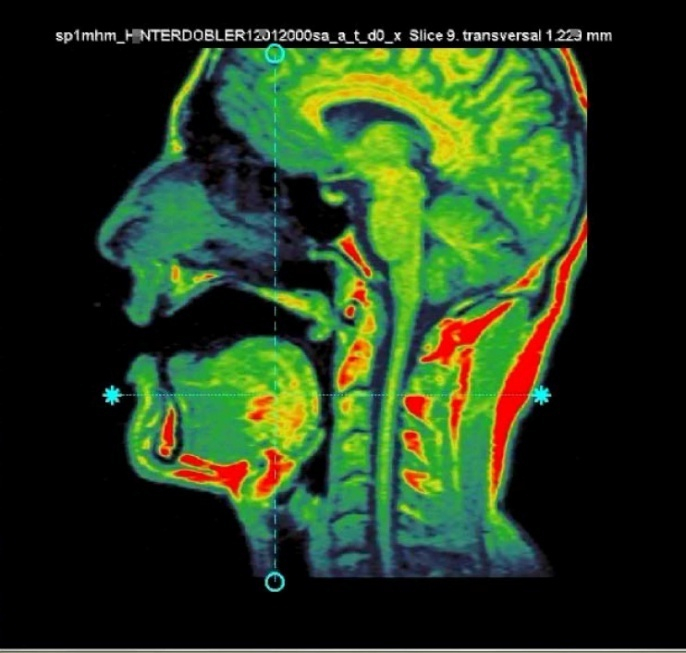
\includegraphics[]{figures/mrt_a.jpg}
    \caption{Vokaltrakt eines Sprechers in der Mittsagittalen. Quelle: Phil Hoole, Institut für Phonetik und Sprachverarbeitung, Ludwig-Maximilians-Universität München.}
    \label{Abb:Vokaltrakt}
\end{figure}


Man kann sich den Vokaltrakt als gekrümmtes Rohr vorstellen, welches vom Sprachschall passiert wird. Um unterschiedliche Laute zu produzieren, werden Verengungen, Verschlüsse oder einfach Veränderungen des Durchmessers an bestimmten Stellen realisiert. In Abbildung~\ref{Abb:Vokaltrakt} gibt es beispielsweise eine Verengung im Rachenraum, während der horizontal liegende Bereich des Vokaltrakts (die Mundhöhle) offen ist.

Im Hals, etwas unterhalb des Kinns, befindet sich der \is{Kehlkopf}Kehlkopf. Im Kehlkopf gibt es zwei Häutchen, die \is{Stimmlippen}\textit{Stimmlippen}.\footnote{Die Stimmlippen werden auch als \textit{Stimmbänder} bezeichnet. Der Begriff ist jedoch irreführend, weil er suggeriert, dass die Stimmlippen wie Gitarrensaiten schwingen.} Beim Atmen werden die Stimmlippen weit voneinander entfernt gehalten, sodass die Luft entweder aus dem Vokaltrakt in die Lunge fließt (beim Einatmen) oder in die umgekehrte Richtung aus der Lunge in den Vokaltrakt (beim Ausatmen). Die Lücke zwischen den Stimmlippen, durch die die Luft fließt, nennt man \textit{Glottis}.\is{Glottis}

Beim \is{Stimmtonerzeugung} Sprechen atmet man in der Regel aus.\footnote{Ausnahmen bilden die ingressiven Laute, bei denen die Luft in Richtung Lunge fließt, und die Clicks (Schnalzlaute), die mit oralem Luftstrommechanismus produziert werden. Bei Interesse empfehlen wir dazu \citet[4.1.9--4.1.10]{Pompino-Marschall2020}. Ingressive Laute gibt es im Deutschen nicht, aber im Hausa, einer tschadischen Sprache, oder auch im Zulu, welches in Südafrika gesprochen wird. Auch Clicks sind im Deutschen keine Phoneme, aber sie existieren in den Khoisansprachen, etwa !Xu. Zulu verfügt ebenfalls über einen Click \citep{UPSIDdatabase}.} Dabei kann mit den Stimmlippen Stimmton erzeugt werden. Die Stimmlippen werden dazu so positioniert, dass sie sich berühren und somit die Luftröhre verschließen. Gleichzeitig strömt Luft aus der Lunge in Richtung Vokaltrakt und erzeugt Druck unter den geschlossenen Stimmlippen. Ist der subglottale Druck (der Druck unter den Stimmlippen)  höher als der supraglottale Druck (der Druck über den Stimmlippen), werden die Stimmlippen aufgesprengt. In diesem Moment kommt es zum sogenannten\is{Bernoulli-Effekt} Bernoulli-Effekt, einem Sogeffekt senkrecht zur Fließrichtung der Luft \citep[32--34, 306]{Pompino-Marschall2020}. Durch diesen Effekt schließen sich die Stimmlippen wieder. Da aus der Lunge jedoch weiter Luft Richtung Vokaltrakt fließt, wiederholt sich dieser Prozess: Der Druck unter der Glottis steigt, die Glottis wird aufgesprengt und schließt sich wieder. Die periodischen Luftdruckunterschiede, die dabei entstehen, nehmen wir als Stimmton wahr.

Besser vorstellbar wird dieser Prozess des Öffnens und Schließens, wenn man ihn an einer Stelle produziert, wo er sichtbar ist, etwa mit den Lippen. Dazu schließt man die Lippen locker und versucht, hindurchzupusten. Die Lippen fangen an, sich periodisch zu öffnen und zu schließen.

Die Geschwindigkeit, mit der sich die Stimmlippen öffnen und schließen, ist einerseits von den anatomischen Gegebenheiten abhängig, kann aber andererseits auch von Sprecherinnen und Sprechern beeinflusst werden. Erwachsene Männer haben im Durchschnitt längere Stimmlippen als erwachsene Frauen. Die Stimmlippen von Kindern sind noch kürzer als die von weiblichen Erwachsenen. Wenn die Stimmlippen länger sind, dauert der oben beschriebene Zyklus von Öffnung und Schließung der Stimmlippen (unter ansonsten gleichen Bedingungen) länger. Männerstimmen öffnen und schließen sich deshalb beim Sprechen etwa 120 mal in der Sekunde (man spricht dann von einer \textit{Grundfrequenz} von 120 Hertz). Frauenstimmen schwingen laut \citet{TraunmuellerEriksson1994} im Mittel knapp doppelt so schnell (etwa 200 mal in der Sekunde) und sind deshalb knapp eine Oktave höher.\footnote{Eine Oktave entspricht einer Verdopplung der Grundfrequenz.} Kinderstimmen können, wie \citet{Reubold2012} zeigt, durch die geringere Länge der Stimmlippen noch deutlich höher sein als Frauenstimmen.

Unabhängig von ihren unterschiedlichen biologischen Voraussetzungen können Sprecherinnen und Sprecher die Stimmhöhe variieren, etwa beim Singen, aber auch beim Sprechen. \citet{Fry1958} zeigt, dass betonte Silben im Allgemeinen mit etwas höherer Grundfrequenz produziert werden als unbetonte. Um einen höheren Stimmton zu produzieren, spannen Sprecherinnen und Sprecher die Stimmlippen an; für eine tiefere Stimme lockern sie sie.

\section{Betonte und unbetonte Silben}\label{section:betonte_unbetonte_Silben}
\is{Betonung}
\is{Akzent!Hauptakzent}
\is{Akzent!Wortakzent}
Im Deutschen hat jedes Wort eine Silbe, die besonders prominent ist. Man nennt diese Silbe die \textit{betonte Silbe}, die Silbe mit dem \textit{Wortakzent} oder die Silbe mit dem \textit{Hauptakzent}. Wenn ein Wort aus nur einer einzigen Silbe besteht, trägt diese Silbe den Hauptakzent. In den folgenden Beispielen ist die betonte Silbe in der orthografischen Form durch Großbuchstaben markiert.

Einige Wörter unterscheiden sich vor allem durch die betonte Silbe voneinander, \zB \textit{GeNUSS} (mit Betonung auf der zweiten Silbe) und \textit{GEnus} (mit Betonung auf der ersten Silbe), oder (mit der Fähre) \textit{Übersetzen} (Betonung auf der ersten Silbe des Verbs) vs. (etwas aus einer Sprache) \textit{überSETzen} (Betonung auf der dritten Silbe). 

Die Betonung ist aber nicht nur relevant, weil damit Wortbedeutungen unterschieden werden. Betonte Silben sind anders aufgebaut als unbetonte (vgl. Kapitel~\ref{kap:Phonologie}). Beispielsweise kommen im norddeutschen Standard einige Vokale -- vor allem die, die in der Schule als \gqq{Langvokale} bezeichnet werden -- nur in betonten Silben vor und andere, wie etwa der sogenannte Schwa-Laut, der zweite Vokal in \textit{Ehe}, nur in unbetonten. 

Orthografisch stehen uns mehrere Mittel zur Verfügung, betonte Silben für Leserinnen und Leser sichtbar zu machen. So verweist ein Dehnungs-\textit{h} immer auf eine betonte Silbe (\textit{SEHne, RAHmen}), eine Doppelkonsonanz kommt in betonten Silben (\textit{Bett, Fall}) oder zwischen betonter und unbetonter Silbe (\textit{SEMmel, RATte}) vor. 

Betonte Silben sind perzeptiv (in der Wahrnehmung) prominenter als unbetonte. Das ist darauf zurückzuführen, dass sie länger und lauter als vergleichbare unbetonte Silben sind (\cite{deJong95}, oder einführend \cite[Kap. 6]{Lodge2009}). Wenn wir etwa die Wörter \textit{FAHRrad} (mit Betonung auf der ersten Silbe) und \textit{VerRAT} (mit Betonung auf der zweiten Silbe) vergleichen, dann ist die erste Silbe in \textit{Fahrrad} länger als die erste Silbe in \textit{Verrat} oder die zweite Silbe in \textit{Fahrrad}. Die zweite Silbe in \textit{Verrat} ist länger als die erste Silbe dieses Wortes oder die zweite Silbe in \textit{Fahrrad}.

Die folgenden Ausführungen zur Betonung im Deutschen orientieren sich an der \citet[619, 631, 635, 902]{Duden2022}. Im Deutschen ist meist die erste Silbe des Stammes betont. \is{Transkription!Betonungszeichen}In der IPA-Transkrip\-tion wird eine betonte Silbe durch ein Hochkomma vor der jeweiligen Silbe gekennzeichnet. Zwischen allen anderen Silben werden Punkte gesetzt:

\ea
\ea \label{ex:Pendel} PENdel \textipa{[\textprimstress pEn.d@l]}
\ex \label{ex:schlafen} SCHLAfen \textipa{[\textprimstress Sla:.f@n]}
\ex \label{ex:lustig} LUStig \textipa{[\textprimstress lUs.tI\c{c}]}
\z 
\z

Bei präfigierten Stämmen\footnote{Präfigierte Stämme sind Wortstämmen mit einem Präfix (schulisch: Vorsilbe, vgl. Abschnitt \ref{subsection:Derivationsaffixe}).} bleibt die Stammbetonung in der Regel erhalten:

\ea
\ea \label{ex:gependelt} gePENdelt \textipa{[g@\textprimstress pEn.d@lt]}
\ex \label{ex:verschlafen} verSCHLAfen \textipa{[f5\textprimstress Sla:.f@n]}
\ex \label{ex:belustigen} beLUStigen \textipa{[b@\textprimstress lUs.ti.g@n]}
\z 
\z
Einige Präfixe ziehen allerdings die Betonung an sich, etwa \textit{un}:

\ea \label{ea:unklug} UNklug \textipa{[\textprimstress PUn.kluk]}
\z 

Verbpartikeln (vgl. Abschnitt~\ref{section:Vpt Bildung}) verschieben den Akzent auf die Partikel.\is{Akzent!Nebenakzent} Dabei kann auf dem Verbstamm ein -- schwächerer -- \textit{Nebenakzent} erhalten bleiben. In der IPA-Transkription steht vor der Silbe mit dem Nebenakzent ein tiefgestelltes Betonungszeichen. Wir zeigen das hier an der Partikel \textit{ein}:
\ea
\ea \label{ex:einpendeln} PENdeln \textipa{[\textprimstress pEn.d@ln]} -- EINpendeln \textipa{[\textprimstress P\t*{aI}n\textsecstress pEn.d@ln]}
\ex \label{ex:einschlafen} SCHLAfen \textipa{[\textprimstress Sla:.f@n]} -- EINschlafen \textipa{[\textprimstress P\t*{aI}n\textsecstress Sla:.f@n]}
\z 
\z

Die meisten Suffixe haben auf die Lage der betonte Silbe keinen Einfluss. Es bleibt bei der Stammbetonung:
\ea
\ea \label{ex:Eitelkeit} EItel \textipa{[\textprimstress P\t*{aI}.t@l]} -- EItelkeit \textipa{[\textprimstress P\t*{aI}.t@l.k\t*{aI}t]}
\ex \label{ex:aenderung} ÄNdern \textipa{[\textprimstress PEn.d5n]} -- ÄNderung \textipa{[\textprimstress PEn.d@.KUN]}
\ex \label{ex:tragbar} DRUCken \textipa{[\textprimstress dKU\.*{k}@n]} -- DRUCker \textipa{[\textprimstress dKU\.*{k}5]}
\z 
\z

Einige Suffixe romanischen Ursprungs ziehen allerdings den Akzent an, etwa \textit{-ei, -erei, -ell} (vgl. Abschnitt~\ref{subsubsection:erei}):
\ea
\ea \label{ex:Kumpanei} BÄCker \textipa{[\textprimstress bE\.*k5]} -- BäckeREI \textipa{[\textsecstress bE\.*k@\textprimstress K\t*{aI}]}
\ex \label{ex:Schweinerei} SCHWEIN \textipa{[Sv\t*{aI}n]}-- SchweineREI \textipa{[\textsecstress Sv\t*{aI}.n@\textprimstress K\t*{aI}]}
\ex \label{ex:maschinell} MaSCHIne \textipa{[ma\textprimstress Si:.n@]}-- maschiNELL \textipa{[ma.Si\textprimstress nEl]}
\z 
\z

Bei Determinativkomposita (vgl. Abschnitt~\ref{subsection:DetKomp}), also Verbindungen aus zwei Stämmen bei denen das Erstglied das Zweitglied genauer bestimmt (\zB \textit{Tischtuch, Straßenbahn, weinrot}), liegt der Hauptakzent auf dem Erstglied. Das Zweitglied trägt einen Nebenakzent. Beide Akzente liegen auf der Silbe, auf der sie vor der Komposition lagen, wie die Beispiele (\ref{ex:Hundeleine}) und (\ref{ex:Verhinderungsdebatte}) zeigen.

\ea
\ea \label{ex:Hundeleine} HUNdeLEIne \textipa{[\textprimstress hUn.d@\textsecstress l\t*{aI}.n@]}
\ex \label{ex:Verhinderungsdebatte} VerHINderungsdeBATte \textipa{[f5\textprimstress hIn.d@.KUNs.de\textsecstress ba\.*t@]}
\z 
\z


Das \is{Trochäus}häufigste Betonungsmuster bei deutschen Zweisilbern ist der \textit{Trochäus}. Ein Trochäus besteht aus einer betonten und einer darauf folgenden unbetonten Silbe. Es gibt viele Wortstämme (vgl. Definition~\ref{def:Wortstamm}, Seite \pageref{def:Wortstamm}), die diesem Muster entsprechen: \textit{HÄUfig, MUSter, ENde, FENSter}. Die meisten Einsilber werden durch die Flexion zu Trochäen: \textit{Band -- Bänder/Bandes, schnell -- schneller/schnelles/schnelle}. Da die zweite Silbe eines Trochäus unbetont ist, können dort nur bestimmte Vokale vorkommen (\zB keine Langvokale). 

Die Trochäen sind im Deutschen so häufig, dass unsere Orthografie bei diesen Wörtern meist auf eine Markierung der Betonung verzichtet und den Trochäus damit sozusagen als Standardfall annimmt. Ein Wort wie \textit{Ende} enthält \zB keine Information darüber, dass das zweite <e> gar nicht als \textipa{[e]} gesprochen wird. Stattdessen sprechen wir dort im norddeutschen Standard den sogenannten Schwa-Laut. Wenn ein Wort kein Trochäus ist, etwa das Wort \textit{binär}, bekommen Leserinnen und Leser über das <ä>, was an dieser Stelle statt <e> geschrieben wird, einen orthografischen Hinweis, dass es sich hier ausnahmsweise nicht um einen Trochäus handelt und der Vokal in der zweiten Silbe deshalb lang zu sprechen ist (\cite[231--232]{FuhrhopPeters2013}, vgl. Abschnitt~\ref{subsec:ääuSchreibungen}).

\section{Konsonanten und Vokale}\label{sec:KonsonantenundVokale}

Konsonanten\is{Konsonant} werden in der Schule häufig als \textit{Mitlaute}\is{Konsonant!Mitlaut} bezeichnet. Damit sind Laute wie \textipa{[s, l, p]} gemeint, die allein keine oder zumindest keine betonbare Silbe bilden können (vgl. Abschnitt~\ref{subsec:Silbe}). Vokale werden in der Schule oft \textit{Selbstlaute}\is{Vokal!Selbstlaut} genannt. Diese Laute sind in betonten Silben obligatorisch. Konsonanten unterscheiden sich von Vokalen in dreierlei Hinsicht: artikulatorisch, akustisch und bezüglich ihrer Position in der Silbe.

\subsection{Artikulatorische Klassifikation}
\textit{Artikulatorisch} gesehen sind Konsonanten Laute, bei denen im Vokaltrakt an mindestens einer Stelle eine Verengung oder ein Verschluss gebildet wird. Bei dem Konsonanten \textipa{[t]} etwa bildet die Zunge einen Verschluss hinter den oberen Schneidezähnen. Die Luft, die aus der Lunge kommt, staut sich hinter dem Verschluss. Der Verschluss wird dann gelöst und man hört ein Verschlusslösungsgeräusch. Bei dem Konsonanten \textipa{[s]} wird an derselben Stelle im Vokaltrakt eine Enge gebildet. Die Luft passiert diese Enge, wobei sie verwirbelt wird. Dadurch entsteht das für diesen Laut charakteristische Rauschen.


Vokale\is{Vokal} sind Öffnungslaute. Bei der Produktion eines Vokals gibt es keine Verengungen oder Verschlüsse im Vokaltrakt. Die Luft kann den Vokaltrakt ungehindert passieren. 

Nach dieser artikulatorischen Einteilung gibt es aber typische und weniger typische Vertreter der beiden Kategorien. Typische Konsonanten sind Laute wie \textipa{[s]} und \textipa{[p]}. Ein typischer Vokal ist \textipa{[a]}. Bei einem untypischen Vokal wie \textipa{[i]} ist die Zunge im Bereich des Gaumens relativ weit oben. Der Vokal \textipa{[i]} unterscheidet sich deshalb artikulatorisch kaum von dem untypischen Konsonanten \textipa{[j]}. Wenn man eine Sequenz wie \textipa{[jiji]} spricht, bewegt sich die Zunge kaum.

\subsection{Akustische Klassifikation}
\textit{Akustisch} gesehen sind Konsonanten Laute, bei denen ein Geräusch entsteht. Unter Geräusch verstehen wir hier Schall mit einem nichtperiodischen Anteil \citep[Kap. 7--9]{Johnson:2003}. Beispiele für Geräusche sind Blätterrascheln, das Ploppen, welches man hört, wenn man eine Flasche entkorkt, oder das Rauschen eines Ventilators. Keine Geräusche in diesem Sinne sind beispielsweise das Tönen eines Martinshorns, Kirchengeläut oder das Signal eines Feuermelders. Bei den Lauten \textipa{[s]} oder \textipa{[p]} ist das Geräusch relativ offensichtlich. Laute wie \textipa{[l]} haben neben einem Stimmanteil auch einen Geräuschanteil. Gut hörbar wird der Geräuschanteil von \textipa{[l]} beim Flüstern, denn beim Flüstern wird kein Stimmton produziert. Ein geflüstertes \textipa{[l]} besteht also nur noch aus dem Geräuschanteil. Vokale sind akustisch dadurch gekennzeichnet, dass sie immer stimmhaft sind und wenig bis gar keinen Geräuschanteil haben. 


\subsection{Position in der Silbe}
Bezüglich der \textit{Position in der Silbe} erkennt man Konsonanten daran, dass sie am Rand der Silbe stehen, während Vokale in der Mitte der Silbe stehen. Betrachten wir dazu die Beispiele in Tabelle~\ref{tab:PositionInDerSilbe}.

\begin{table}
\centering
\caption{Abfolge der Konsonanten und Vokale in den Silben \textit{Tat, Tee, kalt} und \textit{Streik}. Die Vokale stehen in der Mitte, die Konsonanten an den Silbenrändern.\label{tab:PositionInDerSilbe}}
\begin{tabular}{lccc}\lsptoprule
& Konsonanten & Vokale & Konsonanten\\
& (Onset) & (Nukleus) & (Koda)\\\midrule
(1)     & \textipa{t} &\textipa{a:}&\textipa{t}\\
(2)     & \textipa{t} &\textipa{e:}&\\
(3) &\textipa{k} & \textipa{a}& \textipa{lt}\\
(4) & \textipa{StK}& \textipa{\t*{aI}}& \textipa{k}\\\lspbottomrule
\end{tabular}
\end{table}

In der Silbe \textit{Tat} steht das \textipa{[a]} in der Mitte im sogenannten \textit{Nukleus} und die Konsonanten \textipa{[t]} um das \textipa{[a]} herum. Die Position vor dem Vokal nennt man den \textit{Onset},\footnote{engl. \glq Beginn\grq} die hinter dem Vokal die \textit{Koda}\footnote{ital. \glq Schwanz\grq, \glq  Ende\grq} (vgl. Definition~\ref{def:OnsetNukleusKoda}, Seite~\pageref{def:OnsetNukleusKoda}). Würden wir die konsonantischen und vokalischen Positionen austauschen (\textit{ata}) hätte man nicht mehr eine Silbe, sondern zwei. In einer Silbe muss der Vokal also in der Mitte stehen. Das Beispiel \textit{Tee}\footnote{Man spricht hier nur einen Vokal, auch wenn man zwei Vokale schreibt: \textipa{[te:]}} zeigt, dass die Konsonantenposition nach dem Vokal auch leer sein darf. In \textit{kalt} ist die Koda mit mehreren Konsonanten besetzt. In \textit{Streik} steht in der Vokalposition ein sogenannter \textit{Diphthong} (auch: \textit{Zwielaut}, vgl. Abschnitt~\ref{subsec:Diphthonge}), eine Vokalverbindung. Vor diesem Vokal stehen drei Konsonanten, nach dem Vokal einer.\footnote{In Wörtern wie \textit{alt} scheint die erste Konsonantenposition leer zu sein, wir werden aber später sehen, dass das nicht der Fall ist. Hier steht mit dem \is{Knacklaut}glottalen Verschlusslaut (Knacklaut) ein Laut, der orthografisch nicht repräsentiert wird (vgl. Abschnitt~\ref{subsection:Plosive}).}




\begin{Definition}{Vokale und Konsonanten}

\noindent
\is{Konsonant}Konsonanten
\begin{itemize}
    \item werden artikulatorisch durch eine Enge oder einen Verschluss gebildet,
    \item enthalten einen Geräuschanteil,
    \item bilden die Silbenränder.
\end{itemize}
\newpage
\is{Vokal}Vokale
\begin{itemize}
    \item sind Öffnungslaute,
    \item enthalten kaum Geräuschanteil,
    \item bilden Silbennuklei.
\end{itemize}


\end{Definition}



\begin{Exkurs}{Buchstabenkönige: Nuklei im Schriftspracherwerb}
In der vorschulischen Ausbildung und zu Beginn des \is{Schriftspracherwerb}Schriftspracherwerbs werden Vokale häufig \textit{Buchstabenkönige} genannt und manchmal durch eine Krone gekennzeichnet. Die Kinder erfahren bei der Beschäftigung mit den Buchstabenkönigen, dass jede Silbe einen Vokal hat. Für betonte Silben gilt das immer, für unbetonte ist der Vokal nur im Schriftlichen obligatorisch. Verben im Infinitiv (\textit{bitten, reden, laufen}) werden meist ohne Vokal in der zweiten Silbe gesprochen. Im Schriftlichen wird jedoch auch in unbetonten Silben nicht auf den Buchstabenkönig verzichtet.
\end{Exkurs}



\section{Konsonanten}\label{sec:Konsonanten}

Konsonanten können nach \textit{Stimmhaftigkeit, Artikulationsort} und \textit{Artikulationsart} eingeteilt werden. 

\subsection{Stimmhaftigkeit}
\label{sec:Stimmhaftigkeit}
\is{Stimmhaftigkeit}

Konsonanten können stimmhaft oder stimmlos sein. Stimmhaft sind etwa die Konsonanten \textipa{[l]} und \textipa{[m]}. Stimmlos sind die Konsonanten \textipa{[f]} oder der ch-Laut in \textit{ich} \textipa{[\c{c}]}. Während die Stimmlippen bei den stimmhaften Lauten periodisch geöffnet und geschlossen werden, ist die Glottis bei den stimmlosen Lauten weit geöffnet.

Bei der Produktion von stimmhaften Lauten kann die Tonhöhe variiert werden. Wir können etwa ein Lied summen, dann besteht der ganze Text des Liedes aus \textipa{[m]}. Das zeigt, dass \textipa{[m]} ein stimmhafter Laut ist, denn sonst könnten wir die Tonhöhe nicht variieren. Weniger schön, aber zweifellos möglich, ist das auch mit \textipa{[l]}. Mit dem stimmlosen Laut \textipa{[f]} und \textipa{[\c{c}]} hingegen funktioniert das nicht. Auf diese Laute können wir kein Lied singen. Das liegt daran, dass bei diesen Lauten kein Stimmton produziert wird, sie sind stimmlos. Wir können die Tonhöhe daher nicht variieren.

Das Schwingen der Stimmlippen kann man am Hals fühlen. Dazu legt man die Hand an den Kehlkopf und produziert einen stimmhaften Laut, etwa \textipa{[m]}. Am Hals ist jetzt ein Vibrieren spürbar, der Laut ist also stimmhaft. Bei \textipa{[f]} spürt man kein Vibrieren, der Laut ist also stimmlos.\footnote{Beim ch-Laut \textipa{[X]} in \textit{ach} funktioniert dieser Test nicht gut, weil dieser Laut durch eine Enge relativ nah an den Stimmlippen produziert wird, die ebenfalls zu Vibration führen kann. Man kann sich aber überzeugen, dass es sich bei \textipa{[X]} um einen stimmlosen Laut handelt, indem man versucht, auf \textipa{[X]} einen Dreiklang zu singen. Das ist nicht möglich, also ist \textipa{[X]} ein stimmloser Laut.} Bei diesem Test darf man allerdings nicht flüstern, denn beim Flüstern schwingen die Stimmlippen nicht -- eben weil man ansonsten laut sprechen würden.


Die meisten Sprachen haben einen Stimmhaftigkeitskontrast mit zwei Partnern, einem stimmhaften und einem stimmlosen; \textipa{[b]} vs. \textipa{[p]}, \textipa{[g]} vs. \textipa{[k]}. Man spricht bei einem Kontrast mit zwei Partnern von \textit{phonologisch stimmhaften und phonologisch stimmlosen} Lauten. Phonologisch bedeutet hier, dass es eine Opposition zwischen den beiden Lauten in dem jeweiligen Sprachsystem gibt. Wir können die beiden Laute etwa verwenden, um einen Bedeutungskontrast auszudrücken, etwa \textit{Deich -- Teich}. Wie diese Laute in einer Sprache konkret realisiert werden, kann aber von Sprache zu Sprache sehr unterschiedlich sein. Einige Sprachen -- dazu gehört auch der norddeutsche Standard -- nutzen als Unterscheidungsmerkmal die \textit{Aspiration}\is{Aspiration}.

Nativen Sprecherinnen und Sprechern des Deutschen fällt manchmal auf, dass initiales \textipa{[p, t]} oder \textipa{[k]} im Deutschen \gqq{härter} klingt als in romanischen Sprachen. Der Anlaut des deutschen Wortes \textit{Park} klingt \gqq{härter} als der Anlaut des französischen Wortes \textit{parc}. Das französische \textipa{[p]} klingt in etwa wie der Anlaut des deutschen \textit{bar}. Das liegt daran, dass \textipa{[p, t, k]} vor  Vokal zumindest im norddeutschen Standard \textit{aspiriert} sind. Aspiration äußert sich darin, dass nach der Lösung des Verschlusses Luft aus der Lunge entweicht und dabei ein Reibungsgeräusch an der Glottis entsteht, etwa wie bei einem \textipa{[h]}. Wir sprechen also \textipa{[p\textsuperscript{h}a5k]} oder \textipa{[p\textsuperscript{h}a:k]} für \textit{Park}. Im Französischen ist die Aspiration nicht üblich. Aber auch in Teilen Österreichs verzichten die Sprecherinnen und Sprecher auf die Aspiration \citep[58]{DudenAussprache2023}.

Die Laute \textipa{[b, d, g]} klingen in den beiden Sprachen ebenfalls unterschiedlich. Im Französischen sind die Laute \textipa{[b, d, g]} echt stimmhaft. Im Deutschen hängt die Stimmhaftigkeit zu einem großen Teil von der lautlichen Umgebung ab. Zwischen Vokalen sind \textipa{[b, d, g]} stimmhaft, etwa in \textit{eben, Ader, Regen}. Im Anlaut werden sie jedoch entstimmt, sie sind also eigentlich stimmlos, etwa in \textit{Bett, Dom, Gabel} \citep[190--191]{Pompino-Marschall2020}.

Der Unterschied zwischen dem \textipa{[b]} in frz. \textit{belle} und dem \textipa{[p]} in frz. \textit{parc} ist also, dass das \textipa{[b]} stimmhaft und das \textipa{[p]} stimmlos ist. Die Anfangslaute von dt. \textit{Bett} und frz. \textit{parc} sind nahezu identisch. Der Unterschied zwischem dem \textipa{[b]} im dt. \textit{Bett} und dem \textipa{[p]} in dt. \textit{Park} ist, dass das \textipa{[p]} aspiriert ist und das \textipa{[b]} nicht. Wenn man eine engere Transkription anstrebt, müsste diese so aussehen wie in Tabelle~\ref{tab:phonologischphonetischplosiv}.\is{Transkription!entstimmt}

\begin{table}
\caption{Kontrast zwischen phonologischen und phonetische Plosiven\label{tab:phonologischphonetischplosiv}}
\begin{tabularx}{\textwidth}{Xll}\lsptoprule
& Phonologisches p & Phonologisches b\\\hline
französisch& \textit{parc} \textipa{[paKk]} (stimmlos)     &  \textit{belle} \textipa{[bEl]} (stimmhaft)\\
 deutsch &\textit{Park} \textipa{[p\textsuperscript{h}a:k}, \textipa{p\textsuperscript{h}a5k]} (aspiriert)    & \textit{Bett} \textipa{[\r*bEt]} (entstimmt)\footnote{Der Kreis unter dem \textit{b} bedeutet \gqq{entstimmt}.}\\\lspbottomrule
\end{tabularx}
\end{table}
 
Das, was wir im Deutschen orthografisch mit <p, t, k> verschriften, ist jedoch nicht immer aspiriert. Wenn einer dieser Konsonanten auf \textipa{[S]} folgt, den Anfangslaut in \textit{Schule}, dann entfällt die Aspiration, etwa in den Wörtern \textit{spielen} und \textit{Streit}. Dass die fehlende Aspiration wahrgenommen wird, zeigen kindliche Schreibungen wie <schbiln, Schdreit>, wo <b> für das nichtaspirierte \textipa{[p]} und <d> für das nicht aspirierte \textipa{[t]} geschrieben wird. 
 
Eine Auflistung aller IPA-Konsonantensymbole des norddeutschen Standards befindet sich am Ende dieses Abschnitts in Tabelle~\ref{tab:IPA_Kons} auf Seite \pageref{tab:IPA_Kons}. In dieser Tabelle stehen (phonologisch) stimmlose Laute immer links in einer Zelle und (phonologisch) stimmhafte rechts.


\subsection{Artikulationsorte}\label{sec:Artikulationsorte}

Wenn man die Konsonanten \textipa{[t]} und \textipa{[k]} produziert, muss man im Vokaltrakt einen Verschluss bilden. Der Unterschied zwischen den beiden Lauten ist, dass man \textipa{[t]} weiter vorne im Vokaltrakt produziert (relativ nah an den Zähnen) und \textipa{[k]} weiter hinten. \textipa{[t]} und \textipa{[k]} unterscheiden sich also bezüglich des Artikulationsortes -- der Stelle, an der sie gebildet werden. 

Die Artikulationsorte\is{Artikulationsort} der deutschen Konsonanten sind in Abbildung~\ref{Abb:Artikulationsorte} dargestellt. Bevor wir uns den einzelnen Artikulationsorten zuwenden, wird zunächst ein Blick auf den gesamten Artikulationsapparat geworfen. Ganz links in der Abbildung sieht man die Lippen\is{Lippen} (Nr. 1 in der Abbildung). Hinter den Lippen befinden sich die Schneidezähne. Wenn man die Zungenspitze hinter den oberen Schneidezähnen positioniert, kann man die \textit{Alveolen}\is{Alveolen} (den \textit{Zahndamm})\is{Alveolen!Zahndamm} spüren (Nr. 3). Das ist eine Wölbung am Gaumen. Wenn man mit der Zungenspitze nun nach hinten fährt, kann man spüren, dass der Gaumen sich hinter dem Zahndamm nach oben wölbt (Nr. 4). Den Bereich hinter der Wölbung nennt man den \textit{harten Gaumen}\is{Palatum!harter Gaumen} (das \textit{Palatum}, Nr. 5).\is{Palatum} Wenn man die Zunge noch ein bisschen weiter nach hinten wandern lässt (man muss dazu die Zungenspitze irgendwann nach hinten klappen), spürt man, dass der Knochen endet. Das Gewebe fühlt sich weich an. Diesen Bereich nennt man das \textit{Velum}\is{Velum} (den \textit{weichen Gaumen}, Nr. 6).\is{Velum!weicher Gaumen} 

Um einen weiteren Artikulationsort kennenzulernen, braucht man einen Spiegel. Wenn man den Mund weit öffnet, sieht man ganz hinten im Mund eine muskuläre Struktur herunterhängen (Nr. 7). Das ist die \textit{Uvula}\is{Uvula} (das \textit{Zäpfchen}).\is{Uvula!Zäpfchen} Direkt im Hals befindet sich der Kehlkopf mit der \is{Kehlkopf}\textit{Glottis}\is{Glottis} (die \textit{Stimmritze}\is{Stimmritze!Glottis}, Nr. 8). Auch die Glottis ist ein Artikulationsort.


\begin{figure}
    \centering
    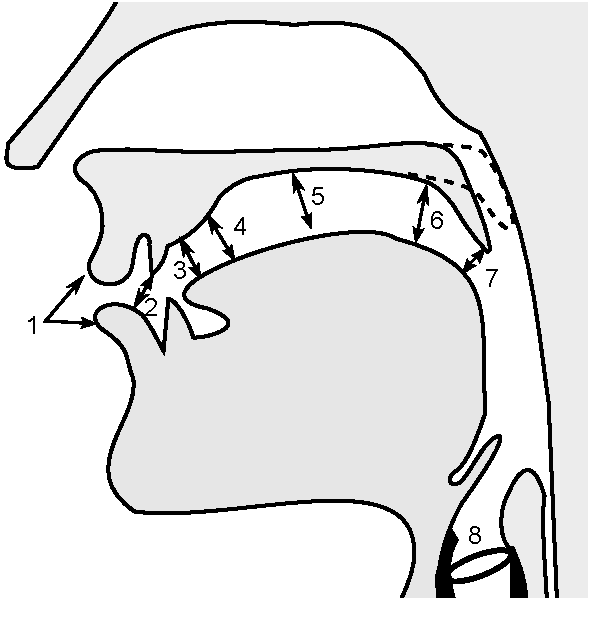
\includegraphics[width=.5\textwidth]{figures/PlaceOfArticulation5.pdf}
    \caption{Artikulationsorte im Deutschen: (1) bilabial, (2) labiodental, (3) alveolar, (4) postalveolar, (5) palatal, (6) velar, (7) uvular, (8) glottal. Das Zäpfchen kann angehoben werden (gestrichelte Linie). Quelle: Tavin, Wikimedia Commons über creative commons licence CC BY 3.0, adaptiert \url{https://commons.wikimedia.org/wiki/File:PlaceOfArticulation.svg}}
    \label{Abb:Artikulationsorte}
\end{figure}

Im Folgenden\is{bilabial} wird untersucht, welche Laute an den einzelnen Orten gebildet werden können. Die Laute zu Beginn der Wörter \textit{Bein}, \textit{Panne} und \textit{Mensch} werden mit beiden Lippen gebildet, was in der Abbildung als (1) dargestellt ist.  Im internationalen phonetischen Alphabet werden diese Laute mit \textipa{[b, p]} und \textipa{[m]} notiert. Diese Laute nennt man \textit{bilabiale} Laute (mit beiden Lippen gebildet).

 Die Wörter \textit{finden}\is{labiodental} und \textit{winden} beginnen mit Lauten, bei denen man die Unterlippe gegen die oberen Schneidezähne legt. Im IPA werden diese Laute \textipa{[f]} und \textipa{[v]} geschrieben. Laute, die mit der Unterlippe und den oberen Schneidezähnen gebildet werden, bezeichnet man als \textit{labiodentale} Laute (Artikulationsort (2) in der Abbildung).

Die Anlaute der Wörter \textit{Nase, leben, tanzen}\is{alveolar} werden mit der Zunge am Zahndamm gebildet (Artikulationsort (3) in der Abbildung). Diese Laute bezeichnet man als \textit{alveolare} Laute. Im IPA werden die Anlaute aus den Beispielwörtern mit \textipa{[n, l, t]} notiert. Im Deutschen gibt es sehr viele alveolare Laute.

Wenn\is{postalveolar} man den Laut \textipa{[s]} lang andauernd bildet und die Zungenspitze dabei ein bisschen zurückzieht, entsteht der Laut \textipa{[S]}, der Anlaut des Wortes \textit{Schule}. Dieser Laut wird hinter den Alveolen gebildet, also \textit{postalveolar} (Artikulationsort (4) in der Abbildung). 

Welche\is{ingressiv} Laute im hinteren Bereich des Mundes an den Artikulationsstellen (5), (6) und (7) gebildet werden, ist schwerer direkt wahrnehmbar. Eine Methode, um die Artikulationsstelle einiger Laute (der sogenannten Frikative, vgl. Abschnitt \ref{subsubsection:Frikative}) wahrnehmbar zu machen, ist \textit{ingressives Sprechen}. Dabei spricht man, während man einatmet. Da die Luft von außerhalb des Vokaltrakts kälter als die Körpertemperatur ist, fühlt sich die Artikulationsstelle kalt an. Wenn man \textipa{[s]} ingressiv produziert, wird es an den Alveolen kalt. Beim \textipa{[\c{c}]}, dem letzten Laut in \textit{ich}, wird es am harten Gaumen kalt. Bei \textipa{[\c{c}]} handelt es sich also um einen \textit{palatalen Laut}\is{palatal} (Artikulationsstelle (5) in der Abbildung). 

Der\is{velar} letzte Laut im Wort \textit{Buch}, \textipa{[x]}, ist ein velarer Laut, er wird am weichen Gaumen gebildet. Auch diese Artikulationsstelle (6) ist erfahrbar, wenn wir den Laut ausgedehnt ingressiv sprechen.

Für\is{uvular} die meisten deutschen Sprecherinnen und Sprecher gibt es perzeptiv keinen Unterschied zwischen dem <ch> in \textit{Buch} und \textit{Bach}. Sie klingen gleich. Nach \textipa{[a]} sprechen wir <ch> jedoch als \textipa{[\textchi]}, einen \textit{uvularen} Laut . Uvulare Laute werden am Zäpfchen gebildet. In der Abbildung entspricht das der Artikulationsstelle (7).

Zu\is{glottal} den \textit{glottalen} Lauten an Artikulationsstelle (8) gehört das \textipa{[h]}, der Anlaut von \textit{Haus}. Dieser Laut wird durch eine Verengung an den Stimmlippen produziert. Durch die Verengung wird die Luft aus der Lunge verwirbelt und erzeugt so das Rauschen, das für diesen Laut typisch ist. 

\subsection{Artikulationsarten}

An manchen Artikulationsorten werden sehr viele Laute gebildet, an den Alveolen etwa \textipa{[s, l, n, t]} und andere. Trotzdem klingen diese Laute sehr verschieden, was nicht nur auf Unterschiede in der Stimmhaftigkeit zurückzuführen ist. Die hauptsächliche Ursache für den unterschiedlichen Klang ist, dass die Laute auf unterschiedliche Arten gebildet werden.


\subsubsection{Plosive}
\label{subsection:Plosive}
\is{Plosiv}

Laute wie \textipa{[p, d, k]} werden gebildet, indem man im Vokaltrakt einen Verschluss produziert. Bei \textipa{[p]}wird der Verschluss an den Lippen produziert, bei \textipa{[d]} an den Alveolen und bei \textipa{[k]} im velaren Bereich. Da während des Verschlusses weiter Luft aus der Lunge Richtung Lippen strömt, erhöht sich der Luftdruck hinter der Verschlussstelle. Wenn der Verschluss gelöst wird, entsteht ein Verschlusslösungsgeräusch\is{burst} (\textit{burst}). Laute, die auf diese Art und Weise gebildet werden, nennt man \textit{Plosive} (vgl. \gqq{Explosion}).

Plosive kann man leicht daran erkennen, dass man sie nicht langanhaltend produzieren kann. Laute wie \textipa{[f], [s]} oder \textipa{[\c{c}]} können wir einige Sekunden lang aushalten, Plosive hingegen nicht, da sie aus Verschluss und Verschlusslösung bestehen und die Verschlusslösung punktuell ist.

Plosive können stimmhaft oder stimmlos sein. Als stimmhaft klassifizieren wir die Plosive \textipa{[b, d, g]}, auch wenn sie nur intervokalisch vollständig stimmhaft sind (vgl. Abschnitt~\ref{sec:Stimmhaftigkeit}). Stimmlos sind die Plosive \textipa{[p, t, k]} und der an der Glottis gebildete \textit{Knacklaut} \textipa{[P]}. 

Der Knacklaut\is{Laute!Knacklaut} ist ein Laut, der keine orthografische Repräsentation hat. Er tritt im Deutschen regelhaft auf. Der Knacklaut ist ein glottaler Plosiv. Bei seiner Bildung sind die Stimmlippen zunächst fest gegeneinander gepresst. Unter der Glottis wird durch die Luft, die aus der Lunge kommt, ein erhöhter Druck aufgebaut. Dieser Druck führt dazu, dass die Glottis aufgesprengt wird, wobei ein Verschlusslösungsgeräusch entsteht. Für die meisten Hörerinnen und Hörer ist das Verschlusslösungsgeräusch (das Knacken) weniger prominent als die Verschlussphase selbst, die sie als kleine Pause wahrnehmen.

Wir betrachten dazu die Wörter \textit{einander} und \textit{ein anderer}. Im \citet{DudenRechtschreibung2024} ist das Wort \textit{einander} mit folgender Silbifizierung angegeben: \uarc{\textit{ei}}\uarc{\textit{nan}}\uarc{\textit{der}}.\footnote{Wir verwenden zur Demonstration der Silbengrenzen hier zunächst die Silbenbögen, die häufig auch in der Grundschule genutzt werden.} Das erste \textipa{[n]} gehört also zur zweiten Silbe. Bei \textit{ein anderer} ist das anders, hier ist die erste Silbengrenze mit der Wortgrenze identisch: \uarc{\textit{ein}} \uarc{\textit{an}}\uarc{\textit{de}}\uarc{\textit{rer}}. Akustisch besteht der Unterschied an der ersten Silbengrenze darin, dass bei \textit{ein anderer} vor dem \textipa{[a]} der Knacklaut gesprochen wird und bei \textit{einander} nicht. Ohne Knacklaut wäre die Silbifizierung \uarc{\textit{ei}}\uarc{\textit{nan}}\uarc{\textit{de}}\uarc{\textit{rer}}.

Den Knacklaut hört man auch vielfach bei nichtsprachlichen Äußerungen, etwa wenn man einen schweren Gegenstand absetzt. Um solche Gegenstände anzuheben, versucht man, den Oberkörper zu stabilisieren. Dazu atmet man ein und verschließt die Lunge durch das Zusammenpressen der Stimmlippen.\footnote{Deshalb kann man beim Anheben eines schweren Möbelstücks kaum atmen.} Wenn man den schweren Gegenstand wieder absetzt, löst man den Verschluss an der Glottis. Dabei entsteht ein Geräusch, so wie man es auch am Anfang eines Stöhnens hört. Das ist der Knacklaut.

Auch viele Sportlerinnen und Sportler produzieren den Knacklaut, zum Beispiel beim Tennisspielen, Kugelstoßen, Diskuswerfen oder Speerwerfen. Auch hier wird zuerst der Oberkörper stabilisiert, indem die Glottis geschlossen wird. Wenn der Ball geschlagen wurde oder die Kugel gestoßen usw. öffnen die Sportlerinnen und Sportler die Stimmlippen. Dabei entsteht der Knacklaut.

Als Sprachlaut wird der Knacklaut in Mittel- und Norddeutschland laut \citet[14, 65f]{DudenAussprache2023} unter folgenden Bedingungen produziert (vgl. Abschnitt~\ref{sec:Epenthese}): 
\begin{itemize}
    \item zu Beginn eines Wortes, wenn das Wort sonst mit Vokal anfangen würde, also \zB bei \textit{Apfel} \textipa{[\textprimstress Pa\.*{\t{pf}}@l]}, \textit{Eis} \textipa{[P\t*{aI}s]}, \textit{anders} \textipa{[\textprimstress Pan.d5s]}, \textit{Ende} \textipa{[\textprimstress PEn.d@]}.
    \item  innerhalb des Wortes am Anfang von betonten Silben, wenn diese sonst mit Vokal beginnen würden, etwa bei bei \textit{überall} \textipa{[\textsecstress Py:.b5\textprimstress Pal]} vor dem \textipa{[a]}, \textit{enteignen} \textipa{[PEnt\textprimstress P\t*{aI}.gn@n]} (vor dem <ei>), \textit{geändert} \textipa{[g@\textprimstress PEn.d5t]}.
\end{itemize}

In Süddeutschland wird der Knacklaut von älteren Generationen seltener produziert, in Österreich und der Schweiz wird er sehr selten gebraucht \citep[66]{DudenAussprache2023}.

Eine sehr saliente\footnote{\textit{Salient} bedeutet, dass der Kontrast hervorstechend ist.} Verwendung des Knacklautes findet man bei \is{geschlechtergerecht} geschlechtergerechter Sprache. Wir vergleichen dazu das Wort \textit{Studentinnen} mit \textit{Student$^\ast$innen} (und den akustisch ähnlich realisierten Formen \textit{Student:innen, StudentInnen, Student\_innen}). Betrachten wir zunächst wieder die Silbifizierung:

\ea
\ea \label{ex:StudentInnen} 
\uarc{Stu} \uarc{den} \uarc{tin} \uarc{nen}
\ex \uarc{Stu} \uarc{dent} \uarc{$^\ast$in} \uarc{nen}
\z
\z

Während die dritte Silbe von \textit{Studentinnen} mit dem Konsonanten \textipa{[t]} anfängt, beginnt die dritte Silbe von \textit{Student$^\ast$innen} orthografisch gesehen mit einem Vokal. An der Stelle des Sternchens, also vor diesem Vokal, wird ein Knacklaut gesprochen. Nach der Regel, die wir oben angegeben haben, wird der Knacklaut nur am Wortanfang oder in betonten Silben eingesetzt. Viele Sprecherinnen und Sprecher betonen bei \textit{Student$^\ast$innen} tatsächlich die dritte Silbe,  wie in Beispiel (\ref{ex:StudentInnen_Transkription}) gezeigt, während sie die weibliche Form in Beispiel (\ref{ex:Studentinnen_Transkription}) auf der zweiten Silbe betonen:

\ea
\ea \label{ex:Studentinnen_Transkription} 
Studentinnen: \textipa{[Stu\textprimstress dEn.tI\.*n@n]}
\ex \label{ex:StudentInnen_Transkription} Student$^\ast$innen: \textipa{[Stu\textsecstress dEnt\textprimstress PI\.*n@n]}
\z
\z



\subsubsection{Frikative}\label{subsubsection:Frikative}
\is{Frikativ}
Frikative sind Laute, bei denen kein Verschluss, sondern eine Enge im Vokaltrakt gebildet wird. Ein Beispiel für einen Frikativ ist der Laut \textipa{[f]}. Bei diesem Laut wird zwischen Unterlippe und oberen Schneidezähnen eine Enge (sogenannte \textit{Konstriktion}\is{Konstriktion}) gebildet, durch die bei der Produktion des Lautes Luft fließt. Die Luft wird beim Passieren der Enge verwirbelt, sodass ein Rauschen entsteht. Dieser Vorgang ist vergleichbar mit der Turbulenzbildung in Flüssen, die Engen passieren.

Ob es tatsächlich zur Verwirbelung und damit zur Rauschbildung kommt, ist, wie \citet{Shadle85} zeigt, vom Verhältnis der Konstriktion zur Geschwindigkeit der Luft abhängig: Wenn man die Konstriktion sehr eng produziert (die Unterlippe also fast schon gegen die Zähne gepresst wird), kann die Fließgeschwindigkeit der Luft geringer sein, um Rauschen zu produzieren. Wenn die Konstriktion eher weit ist, muss die Geschwindigkeit der Luft höher sein, um Rauschen zu erzeugen. Ist weder das eine noch das andere gegeben (die Konstriktion ist weit und die Fließgeschwindigkeit niedrig), kann kein Rauschen erzeugt werden.

Eine\is{Sibilant} besondere Klasse innerhalb der Frikative bilden die \textit{Sibilanten} \textipa{[s, z, S]}, die in den Anlauten der Wörter \textit{Skelett} \textipa{[ske\textprimstress lEt]}, \textit{Sonne} \textipa{[\textprimstress zO\.*{n}@]}\footnote{Diese Aussprache empfiehlt das \citet[139]{DudenZweifelsfaelle2021}. Im Süddeutschen, der Schweiz und Österreich spricht man jedoch meist \textipa{[\textprimstress sO\.*{n}@]} \citep[74]{DudenAussprache2023}, siehe auch Stefan Kleiner: \textit{Atlas zur Aussprache des deutschen Gebrauchsstandards (AADG)}. \url{https://prowiki.ids-mannheim.de} (Zugriff: 28.08.2025) zum Stichwort \textit{s im Anlaut}.} und \textit{Schule} \textipa{[\textprimstress Su:.l@]} vorkommen. Ein weiterer Sibilant ist das \is{nativ} nichtnative\footnote{\textit{Nativ} bedeutet, dass diese Laute im nativen (nicht fremdsprachlichen) Wortschatz vorkommen. \textipa{[s]} kommt \zB im Erbwort \textit{messen} vor und ist deshalb nativ. Der Anlaut des Wortes \textit{Thinktank} \textipa{[\texttheta]} ist kein nativer Laut, denn er kommt nur in Fremdwörtern vor, genauso wie \textipa{[Z]}. Den Stamm \textit{nativ} findet man auch in \textit{native speaker, digital native}.}  \textipa{[Z]}, welches in  \textit{Genie} \textipa{[Ze\textprimstress ni:]} vorkommt. Sibilanten sind Laute, bei denen der Luftstrom zunächst -- wie bei allen Frikativen -- eine Konstriktion passiert, hinterher aber noch gegen ein Hindernis geleitet wird. Dieses Hindernis sind die Schneidezähne. \citet{Shadle1991} zeigt, dass an den Schneidezähnen eine weitere Verwirbelung der Luft erfolgt, sodass Sibilanten sich durch ein besonders intensives hochfrequentes Rauschen auszeichnen.\footnote{Am Telefon kann man \textipa{[s]} und \textipa{[f]} nicht immer gut unterscheiden. Wenn man ein Wort mit <s> buchstabiert, versteht der Kommunikationspartner häufig <f>. Das liegt daran, dass über das Telefon nur Frequenzen bis 3,4kHz übertragen werden. Die charakteristischen Eigenschaften des Lautes \textipa{[s]} (das hochfrequente Rauschen) liegen aber über 3,4kHz und werden deshalb nicht übertragen. In fließender Rede fällt das jedoch nicht auf, weil unser Gehirn die fehlenden Informationen ergänzt.}


\begin{Exkurs}{Warum klingen \textipa{[s]} und \textipa{[z]} bei Kindern manchmal gelispelt?}
\label{Exkursgelispeltess}

\noindent Die wichtige Rolle der Schneidezähne bei den Sibilanten wird deutlich, wenn man versucht, Sibilanten mit großem Abstand zwischen den Schneidezähnen zu produzieren (also mit tiefem Kiefer). Sprechen Sie dazu zunächst ein paarmal \textit{lalala} und versuchen Sie dann, bei \textipa{[l]} anzuhalten. Legen Sie dabei einen Finger an Ihr Kinn, um die Kieferposition zu kontrollieren. Versuchen Sie nun, zu einem \textipa{[s]} zu wechseln und dabei die Kieferposition unverändert zu lassen. Wenn Ihnen das gelingt, sollte das \textipa{[s]} weniger intensiv, möglicherweise \gqq{gelispelt} klingen. Das liegt daran, dass Sie den Luftstrom nun nicht mehr gegen die unteren Schneidezähne leiten können.

Möglicherweise bewegen Sie auch ganz automatisch den Kiefer nach oben. Dann klingt das \textipa{[s]} normal, eben weil der Luftstrom gegen die unteren Schneidezähne geleitet wird und dort weitere Turbulenzen entstehen.

Nun aber zur Ausgangsfrage: Warum klingen \textipa{[s]} und \textipa{[z]} bei Kindern, vor allem im Alter von 6--7 Jahren, manchmal gelispelt? Diesen Kindern fehlen häufig ein oder mehrere Schneidezähne, weil sie gerade ihr Milchgebiss verlieren. Dadurch muss der Luftstrom nicht, wie bei Menschen mit vollständigem Gebiss, ein zweites Hindernis passieren. Das führt (wie bei dem Experiment eben) zu einem weniger intensiven Rauschen. Wenn die Kinder vor dem Zahnverlust nicht gelispelt haben, werden sie die Laute aller Wahrscheinlichkeit nach unauffällig sprechen, sobald das Gebiss wieder vollständig ist.
\end{Exkurs}

\largerpage
Sobald Sprecher(innen) des Deutschen alphabetisiert sind,\is{Laute![s]} finden sie es oft schwierig, \textipa{[s]} und \textipa{[z]} zu unterscheiden. Das liegt unter anderem daran, dass die Schreibung wenig Aufschluss über die Lautung gibt. \textipa{[s]} kann als <s, ss> oder <ß> (\textit{mie\underline{s}, vermi\underline{ss}en, Fü\underline{ß}e}) geschrieben werden. \textipa{[z]} wird immer <s> geschrieben (\textit{We\underline{s}en}). Um den Unterschied zwischen den Lauten \textipa{[s]} und \textipa{[z]} zu verdeutlichen, benutzen wir eine Terminologie aus der Kinder-Logopädie (\zB \cite[45ff]{FoxBoyeretal2015}). \textipa{[s]} wird in der Kinder-Logopädie \gqq{Schlangenlaut} genannt, weil man mit diesem Laut das Zischen einer Schlange imitieren kann. Das stimmhafte \textipa{[z]} wird als \gqq{Bienenlaut} bezeichnet -- das Summen einer Biene wird imitiert.  

Viele Laute können in jeder Position vorkommen, das \textipa{[p]} zum Beispiel initial in \textit{Panne} \textipa{[\textprimstress pa\.*n@]}, medial in \textit{Happen} \textipa{[\textprimstress ha\.*p@n]}, alternativ \textipa{[\textprimstress ha\.*p\s{m}]}, und final in \textit{stopp} \textipa{[StOp]}. Das ist bei den beiden alveolaren Frikativen \textipa{[s]} und \textipa{[z]} nicht so. Im norddeutschen Standard kommt das \textipa{[s]} nur medial, \zB in \textit{Masse} \textipa{[\textprimstress ma\.*s@]} und \textit{Grüße} \textipa{[\textprimstress gKy:s@]} und final, \zB  in \textit{Bus} \textipa{[bUs]}, \textit{Bass} \textipa{[bas]} und \textit{Gruß} \textipa{[gKu:s]} vor. Initial ist es sehr eingeschränkt. Es kommt in Fremdwörtern wie \textit{Cent} \textipa{[sEnt]} und in Konsonantenverbindungen wie in \textit{Skandal} \textipa{[skan\textprimstress da:l]} vor. Ansonsten ist es auf den bairischen und schweizer Sprachraum begrenzt. Das Wort \textit{Sache} etwa wird im norddeutschen Standard \textipa{[\textprimstress za\.*x@]} gesprochen, im bairischen und schweizer Raum aber \textipa{[\textprimstress sa\.*x@]} \citep[74]{DudenAussprache2023}.

Das \textipa{[z]}\is{Laute![z]} ist ebenfalls nicht in jeder Position zu finden. Es kommt initial vor, etwa in \textit{Sand} \textipa{[zant]} oder \textit{sieben} \textipa{[\textprimstress zi:.b@n]}, alternativ \textipa{[\textprimstress zi:b\s{m}]}, aber es steht auch medial, etwa in \textit{Faser} \textipa{[\textprimstress fa:.z5]} oder \textit{lesen} \textipa{[\textprimstress le:z@n]}, alternativ \textipa{[\textprimstress le:z\s{n}]}. Aufgrund der Auslautverhärtung (vgl. Abschnitt~\ref{sec:Auslautverhaertung}) kommt \textipa{[z]} aber nicht final vor. Man spricht zwar \textit{Mäuse} \textipa{[\textprimstress m\t*{OI}.z@]}, aber \textit{Maus} \textipa{[m\t*{aU}s]}, nicht \textipa{[m\t*{aU}z]}.

Der\is{Laute!ch-Laute} palatale Frikativ \textipa{[\c{c}]}, der velare \textipa{[x]} und der uvulare \textipa{[X]} werden orthografisch alle als <ch> repräsentiert. Auch diese Laute kommen nur in bestimmten Umgebungen vor, der Laut  \textipa{[\c{c}]} etwa in den folgenden drei:
\begin{itemize}
    \item nach den sogenannten Vorderzungenvokalen \textipa{[i, I, y, Y, e, E, \o, \oe]} (vgl. Abschnitt~\ref{sec:Vokale}), \zB in \textit{Bücher} \textipa{[\textprimstress bY:.\c{c}5]} oder \textit{Becher} \textipa{[\textprimstress bE\.*{\c{c}}5]}
    \item nach Konsonanten, \zB in \textit{Milch} \textipa{[mIl\c{c}]}
    \item zu Beginn eines Morphems\footnote{Ein Morphem ist eine bedeutungstragende Einheit, auch: Wortbaustein (vgl. Abschnitt~\ref{section:Einheiten Wortbildung}, \pageref{section:Einheiten Wortbildung}, Definition~\ref{def:Morphem}.)} \zB in \textit{Häuschen} \textipa{[h\t*{OI}s.\c{c}@n]}.
\end{itemize} 

Der velare Frikativ \textipa{[x]} wird nach den Hinterzungenvokalen \textipa{[u, o]}, \zB in \textit{Buch} \textipa{[bu:x]} und \textit{hoch} \textipa{[ho:x]} gesprochen. Der uvulare Laut \textipa{[X]} wird nach \textipa{[a, U, O]} gesprochen: \textit{Dach} \textipa{[daX]}, \textit{Bucht} \textipa{[bUXt]}, \textit{Koch} \textipa{{kOX}} (vgl. Abschnitt~\ref{sec:Allophone}, \cite[202]{Pompino-Marschall2020}).

Die stimmhafte Variante des uvularen Frikativs \textipa{[X]} ist \textipa{[K]}. Dieser Laut kann initial im Wort \textit{Raum} \textipa{[K\t*{aU}m]} gesprochen werden. Laut \citet[52]{DudenAussprache2023} ist \textipa{[K]} die häufigste Art, den r-Laut zu sprechen und -- außer in Teilen der Schweiz -- überall gebräuchlich. Im Gegensatz zu den anderen beiden r-Varianten ist \textipa{[K]} nicht gerollt, sondern am Zäpfchen gerieben (vgl. Abschnitt~\ref{sec:Vibranten}).

Auch das \textipa{[h]}\is{Laute![h]} ist ein Frikativ. Es wird an der Glottis produziert. Die Engebildung erfolgt bei diesem Laut zwischen den Stimmlippen. Die Stimmlippen nähern sich dazu einander an, jedoch ohne dass die Glottis geschlossen wird.




\subsubsection{Nasale}\label{subsec:Nasale}

Die Wörter \textit{Nase} und \textit{Masse} beginnen mit einem Nasal.\is{Nasal} Bei Nasalen wird der Mund an einer Stelle verschlossen - bei \textipa{[m]} an den Lippen und bei \textipa{[n]} an den Alveolen. Das Velum wird gleichzeitig gesenkt, sodass die Luft nicht durch den Mund, sondern durch die Nase entweicht. 

Artikulatorisch gesehen sind Nasale den Plosiven sehr ähnlich, weil auch bei den Plosiven der Mund an einer Stelle verschlossen wird. Abbildung~\ref{fig:Plosiv_Nasal} zeigt auf der linken Seite einen Sagittalschnitt für \textipa{[p]} und auf der rechten für \textipa{[m]}. Der einzige Unterschied zwischen den beiden Konfigurationen ist das Velum, welches bei \textipa{[p]} gehoben ist und bei \textipa{[m]} gesenkt, sodass die Luft durch die Nase entweichen kann. Im Mundraum unterscheiden sich die Laute nicht.\is{Velum}

\begin{figure}
     \centering
     \begin{subfigure}[b]{0.4\textwidth}
         \centering
         
\includegraphics[width=\textwidth]{figures/Voiceless_bilabial_plosive.svg.png}
         \caption{Bilabialer Plosiv \textipa{[b]} oder \textipa{[p]}}
         \label{fig:bilabialer_Plosiv}
     \end{subfigure}
     \hfill
     \begin{subfigure}[b]{0.4\textwidth}
         \centering
         
\includegraphics[width=\textwidth]{figures/Voiced_bilabial_nasal.svg.png}
         \caption{Bilabialer Nasal \textipa{[m]}}
         \label{fig:bilabialer_Nasal}
     \end{subfigure}
        \caption{Artikulatorische Konfigurationen der Plosive und Nasale. Quelle: Tavin, Wikimedia Commons über creative commons licence CC BY-SA 4.0, \url{https://commons.wikimedia.org/wiki/File:Voiceless\_bilabial\_plosive.svg}, \url{https://commons.wikimedia.org/wiki/File:Voiceless\_bilabial\_nasal.svg}}
        \label{fig:Plosiv_Nasal}
\end{figure}



Ob ein Laut ein Nasal ist, kann man feststellen, indem man die Nasalpassage verschließt (sich also die Nase zuhält). Wenn der Laut dann nicht mehr gebildet werden kann, handelt es sich um einen Nasal. Laute wie \textipa{[p, s, l]} können mit geschlossener Nase problemlos gebildet werden -- weil sie keine Nasale sind. Die Nasale \textipa{[m]} in \textit{Mensch} \textipa{[mEnS]}, \textipa{[n]} in \textit{nehmen} \textipa{[\textprimstress ne:.m@n]}, alternativ \textipa{[\textprimstress ne:.m\s{n}]} oder \textipa{[\textprimstress ne:.m:]}, und \textipa{[N]}, der letzte Laut in \textit{eng} \textipa{[PEN]}, sind jedoch mit geschlossener Nase nicht produzierbar.

Ein weiteres Indiz dafür, dass die Luft bei den Nasalen tatsächlich durch die Nase fließen muss, liefern Sprecherinnen und Sprecher, die erkältet sind. Wenn die Nase zugeschwollen ist, klingen die Nasale perturbiert.

Nasale sind eher leise Laute. Das liegt einerseits daran, dass der Schall in der Nasenhöhle gedämpft wird. Andererseits enthält das Nasalspektrum sogenannte \textit{Antiformanten}\is{Antiformant}. Wenn die Luft bei der Produktion von Vokalen von der Glottis bis zu den Lippen fließt, werden abhängig von der Zungen- und Lippenposition bestimmte Frequenzbereiche des Schalls verstärkt. Diese Bereiche nennt man Resonanzen oder \textit{Formanten}\is{Formant}. Wenn der Schall von der Glottis bis zu den Nasenlöchern fließt, entstehen ebenfalls Formanten. Die verschlossene Mundhöhle, die als Seitenarm der Passage von der Glottis bis zu den Nasenlöchern fungiert, schwächt einzelne Frequenzbereiche allerdings ab, anstatt sie zu verstärken. Dadurch entstehen Antiformanten, das sind Frequenzbereiche mit niedriger Amplitude \citep[Kap.9]{Johnson:2003}. 

Die Antiformanten machen das Nasalspektrum wenig charakteristisch. Deshalb sind Nasale schwer voneinander zu unterscheiden. Besonders die Laute \textipa{[m]} und \textipa{[n]} unterscheiden die meisten Hörerinnen und Hörer nicht auditiv, sondern visuell: Sie schauen auf die Lippen des Sprechers oder der Sprecherin und können so feststellen, ob es sich um einen bilabialen oder alveolaren Nasal handelt. Sehbehinderte Hörerinnen und Hörer finden es häufig schwierig, diese beiden Laute ohne Kontext zu unterscheiden. Auch beim Schriftspracherwerb kann es deshalb zu Verwechslungen von <m> und <n> kommen.

Aber auch mit durchschnittlichem Sehvermögen lernen wir die beiden Laute, wenn sie in weniger prominenten Positionen stehen (etwa als Flexionsendung), häufig erst über die Schrift zu unterscheiden. Davon zeugen die Äußerungen von Kindern zu Beginn des Schriftspracherwerbs in (\ref{ex:nstattm1}) und (\ref{ex:nstattm2}). Die entscheidenden Stellen sind durch Großbuchstaben markiert.

\ea
\ea \label{ex:nstattm1} Schriftliche Äußerung:\\ <aber du must noch ein bischen merr an deineN stiel arbeiten> (Schülerin der 2. Klasse, 8 Jahre alt\footnote{Karlsruhe Childen's Text Corpus, \citet{Lavalleyetal2015}})
\ex \label{ex:nstattm2} Mündliche Äußerung:\\ \textit{Ipalat, Ipalat, tut deN Hals gut, Ipalat} (Schüler der 1. Klasse, 6 Jahre alt, Hörbeleg auf einem Schulhof)
\z
\z
Diese Fehler basieren in der Regel nicht auf ungenügenden Flexionskenntnissen. Kinder in diesem Alter produzieren nämlich den Dativ femininer Substantive, wo keine Opposition zwischen \textipa{[n]} und \textipa{[m]} besteht, in der Regel korrekt: \textit{an deinER Geschichte arbeiten} (nicht \textit{deine}), \textit{tut DER Nase gut} (nicht \textit{die}).

Die\is{Vokal!nasal} nasalen Konsonanten dürfen nicht mit den nasalen Vokalen verwechselt werden. Der Unterschied zwischen nasalen Konsonanten und nasalen Vokalen besteht darin, dass es bei den Konsonanten einen vollständigen oralen Verschluss gibt. Bei nasalen Vokalen hingegen fließt die Luft gleichzeitig durch Mund und Nase \citep[163--166]{Johnson:2003}.

Nasale Vokale produzieren im deutschen Sprachraum nur wenige Sprecherinnen und Sprecher überhaupt, und dann nur in französischen Lehnwörtern wie etwa \textit{Restaurant} \textipa{[KEs.to\textprimstress r\~{\textscripta}]} oder \textit{Balkon} \textipa{[bal\textprimstress k\~{O}]}. Die meisten Sprecher(innen) neigen eher dazu, nasalierte Vokale in Fremdwörtern einzudeutschen: In Nord- und Mitteldeutschland \zB indem ein velarer nasaler Konsonant gesprochen wird, etwa \textit{Balkon} \textipa{[bal\textprimstress kON]}, \textit{Restaurant} \textipa{[KEs.to\textprimstress KaN]} oder \textipa{[KEs.to\textprimstress KON]}, \textit{Ragout fin} \textipa{[Ka.gu\textprimstress fEN]} \citep[35, 69]{DudenAussprache2023}. In Österreich und der Schweiz wird statt des \textipa{[N]} am Ende eher \textipa{[n]} gespochen, bei \textit{Balkon}  also \textipa{[bal\textprimstress ko:n]}.\footnote{Stephan Elspaß \& Robert Möller: \textit{Atlas zur deutschen Alltagssprache (AdA)}. \url{https://www.atlas-alltagssprache.de} (Zugriff am 28.08. 2025), Stefan Kleiner: \textit{Atlas zur Aussprache des deutschen Gebrauchsstandards (AADG)}. \url{https://prowiki.ids-mannheim.de} (Zugriff am 28.08.2025)}


\subsubsection{Vibranten}
\label{sec:Vibranten}
\is{Vibrant} Vibranten werden auch als gerollte Laute bezeichnet. Ein typisches Beispiel ist das gerollte Zungenspitzen-r. Die Produktion von Vibranten ist in gewisser Weise vergleichbar mit der des Stimmtons (vgl. Abschnitt~\ref{sec:Stimmhaftigkeit}): Es wird ein Verschluss gebildet und der Luftdruck hinter dem Verschluss steigt so lange, bis der Verschluss aufgesprengt wird. Beim Aufsprengen fließt die Luft durch die Artikulationsstelle. Durch die Stömung nimmt der Luftdruck an der Artikulationsstelle ab und es erfolgt ein Sog in einem Winkel von 90 Grad zur Strömung (\isi{Bernoulli-Effekt}). Dadurch  entsteht sofort ein weiterer Verschluss. Bei einem in fließender Rede produzierten Vibranten kommt es meist zu 2--3 Verschlusslösungen.

Im Unterschied zur Produktion von Stimmton, die im Kehlkopf an der Glottis stattfindet, werden Vibranten in der Mundhöhle produziert. Außerdem erfolgt das Öffnen und Schließen mit einer viel geringeren Frequenz als beim Stimmton. Wir können bei Vibranten deshalb akustisch einzelne Verschließ- und Öffnungsereignisse wahrnehmen, während wir Stimmton nicht als eine Abfolge von Öffnen und Schließen, sondern als Ton wahrnehmen.

Um einen Vibranten zu produzieren, benötigt man einen Artikulator, der sich sehr schnell bewegen kann. Dafür kommen nur die Lippen, die Zungespitze und die Uvula in Frage. Mit den Lippen können wir, wie in Abschnitt~\ref{sec:Vokaltrakt} angesprochen, einen bilabialen Vibranten produzieren. Dieser Laut wird im Deutschen allerdings nur in nonverbaler Funktion verwendet.

Viele Sprecherinnen und Sprecher produzieren den r-Laut als Vibranten. Dabei gibt es zwei Möglichkeiten, das Zungenspitzen-r und das gerollte Zäpfchen-r. Das Zungenspitzen-r \textipa{[r]} produziert man, indem man die Zungenspitze gegen die Alveolen legt -- wie für ein \textipa{[t]} -- und dann Luft durchbläst. Dabei muss die Zungenspitze aber so entspannt sein, dass sie anfängt zu vibrieren (ansonsten entsteht ein \textipa{[s]}). Diese Realisation findet sich vor allem im süddeutschen und österreichischen Raum.

Das gerollte Zäpfchen-r \textipa{[\;R]} produziert man, indem man den Zungenrücken an die Uvula (das Zäpfchen) legt. Dann bläst man Luft durch diesen Verschluss, sodass die Uvula zu vibrieren beginnt. Das gerollte Zäpfchen-r kommt vor allem vor, wenn etwas besonders hervorgehoben werden soll, \zB in kontrastierenden Kontexten: \textit{Ich habe nicht Leiter gesagt, sondern Rrreiter.}

\subsubsection{Approximanten}

\is{Approximant}Approximanten werden auch \is{Approximant!Halbvokal} \textit{Halbvokale} genannt. Das liegt daran, dass sie artikulatorisch und akustisch den Vokalen sehr nahe sind. Im Deutschen gibt es nur einen Approximanten, das \textipa{[j]}, wie in \textit{jung} \textipa{[jUN]}. Der Begriff Approximant ist darauf zurückzuführen, dass ein Artikulator sich an eine Artikulationsstelle annähert (lat. \textit{approximare} 'sich annähern'), ohne jedoch eine geräuschbildende Enge zu produzieren.

Approximanten\is{Frikativ} werden also durch eine Verengung im Vokaltrakt produziert; allerdings ist die Verengung nicht so eng, dass es zu Turbulenzen kommt. Im Unterschied zu den Frikativen, die auch durch eine Engebildung verursacht werden, wird die Luft bei den Approximanten nicht verwirbelt und es entsteht kein intensives Rauschen. Den Luftstrom bei den Approximanten können wir uns vorstellen wie einen Fluss, der an einer Stelle etwas eingeengt wird. Das Wasser fließt an der Stelle etwas schneller, aber es entstehen keine Strudel \is{laminarer Luftstrom}(laminarer Luftstrom). Der Luftstrom bei einem Frikativ ist eher vergleichbar mit einem Fluss, der stark eingeengt wird, wodurch es zur Strudelbildung kommt \is{turbulenter Luftstrom}(turbulenter Luftstrom). 

Wir können den Unterschied zwischen Frikativen und Approximanten gut nachvollziehen, indem wir die Laute \textipa{[j]}, wie im Anlaut von \textit{jeder}, und \textipa{[\c{c}]}, wie im Auslaut von \textit{ich}, vergleichen. Wenn wir eine Sequenz wie \textipa{[\c{c}j\c{c}j]} sprechen, ist der Hauptunterschied der Stimmton, den wir für \textipa{[j]} brauchen, für den Frikativ jedoch nicht. Um das Rauschen für den Frikativ zu produzieren, müssen Sprecherinnen und Sprecher entweder die Konstriktion\is{Konstriktion} etwas verengen (die Zunge geht nach oben) oder die Fließgeschwindigkeit erhöhen. Letzteres erreicht man, indem man Druck auf die Lunge ausübt \citep[Abschnitt 1.2]{Pompino-Marschall2020}. Dass man das tut, merkt man daran, dass man für \textipa{[\c{c}]} die Bauchmuskeln stärker anspannt.

Bei \textipa{[j]}\is{Vokal} erfolgt die Verengung im palatalen Bereich. In Abschnitt~\ref{sec:KonsonantenundVokale} wurde gezeigt, dass das \textipa{[j]} sich artikulatorisch kaum vom Vokal \textipa{[i]} unterscheidet. Man zählt den Approximanten trotzdem nicht zu den Vokalen, weil er nur im Onset einer Silbe stehen kann (also vor dem Vokal) und den Vokal nicht ersetzen kann (vgl. Abschnitt~\ref{sec:KonsonantenundVokale}). Es gibt also Silben, die mit \textipa{[j]} beginnen: \textit{Jugend} \textipa{[\textprimstress ju:.g@nt]}, \textit{Joch} \textipa{[jOX]}, \textit{Koje} \textipa{[\textprimstress ko:.j@]}. Außerdem kann das \textipa{[j]} -- vor allem im nichtnativen\is{nativ} Wortschatz -- auch einem Konsonanten folgen, \zB in \textit{tja, Bjarne, Kjelt},\footnote{Wenn der vorangehende Laut stimmlos ist, überträgt sich dieses Merkmal auf das \textipa{[j]}, sodass der Laut entstimmt wird und damit dem \textipa{[\c{c}]} sehr ähnlich wird.} aber es kann ohne Vokal keine Silbe bilden. Im Deutschen kann \textipa{[j]} nicht in der Koda einer Silbe stehen.

\subsubsection{Laterale}
\is{Lateral}
\largerpage
Die Engebildung bei Frikativen und Approximanten erfolgt zentral, also in der Mitte des Vokaltrakts. Wir können das für uns erfahrbar machen, indem wir \is{ingressiv}ingressiv sprechen, also sprechen, während wir einatmen (vgl. Abschnitt~\ref{sec:Artikulationsorte}). Wenn man \textipa{[\c{c}]} ingressiv spricht, merkt man, dass es an der Artikulationsstelle im palatalen Bereich in der Mitte des Gaumens kalt wird. 

Laterale\footnote{Singular: \textit{der Lateral}, Plural: \textit{die Laterale}} sind Laute mit \textit{seitlicher Engebildung} \citep[183]{Pompino-Marschall2020}. Der einzige Lateral im Deutschen ist das \textipa{[l]}. Bei diesem Laut liegt die Zunge an der linken oder rechten Seite des Gaumens an. Auf der anderen Seite des Gaumens fließt die Luft entlang. Wenn man \textipa{[l]} ingressiv spricht, sollte man -- wenn die Artikulationsposition wirklich so ist wie beim egressiven Sprechen -- spüren, dass es auf einer Wangeninnenseite kälter wird als auf der anderen.

In \is{Approximant!lateral}einigen Lehrwerken werden die Laterale zu den Approximanten gezählt und bilden dort die Untergruppe der lateralen Approximanten. Die Laterale unterscheiden sich von den zentralen Approximanten\is{Approximant!zentral} tatsächlich nur darin, dass die Enge bei den Lateralen seitlich ist. Das Verhalten des Luftstroms (keine Turbulenzen beim Passieren einer Enge) ist bei den beiden Lautklassen gleich.


\subsubsection{Affrikaten}\label{sec:Affrikaten}
\is{Affrikate}
Zu den Affrikaten\footnote{Singular: \textit{die Affrikate}, Plural: \textit{die Affrikaten}} zählen im Deutschen \textipa{[\t{pf}]}, wie in \textit{Apfel} \textipa{[\textprimstress Pa\.*{\t{pf}}@l]}, \textipa{[\t{ts}]}, wie in \textit{Katze} \textipa{[\textprimstress ka\.*{\t{ts}}@]} und \textipa{[\t{tS}]} wie in \textit{Gletscher} \textipa{[\textprimstress glE\.*{\t{tS}}5]}. Affrikaten sind \textit{homorgane\is{homorgan} Plosiv-Frikativ-Verbindungen}. \is{homorgan}Homorgan bedeutet, dass beide Laute, der Plosiv und der Frikativ, an etwa derselben Stelle gebildet werden.  Im nichtnativen Wortschatz gibt es zusätzlich zu den drei genannten Affrikaten\is{Laute![d͡ʒ]} noch das \textipa{[\t{dZ}]}, das etwa in \textit{Gin} \textipa{[\t{dZ}In]} vorkommt.\footnote{Die nichtnative Affrikate\textipa{[\t{dZ}]} ist nicht gleichzusetzen mit dem ebenfalls nichtnativen Frikativ \textipa{[Z]}. Die Affrikate spricht man in \textit{Job} \textipa{[\t{dZ}Ob]} (wenn man es englisch ohne Auslautverhärtung spricht), \textit{Dschungel} \textipa{[\textprimstress \t{dZ}U\.*N@l]}, \textit{Gender} \textipa{[\t{dZ}En.d5]}. Den Frikativ spricht man in \textit{Journal} \textipa{[ZUK\textprimstress na:l]} oder \textit{Gelée} \textipa{[Ze\textprimstress le:]}.}


Für den Schriftspracherwerb relevant sind die Affrikaten aus verschiedenen Gründen. Die Affrikate \textipa{[\t{pf}]} wird im Onset einer Silbe in nichtstandardsprachlichen Varianten Mittel- und Norddeutschlands häufig auf den Frikativ \textipa{[f]} reduziert \citep[693]{DudenAussprache2023}, was zu kindlichen Schreibungen wie <feat> für \textit{Pferd} führt.

Die Affrikate \textipa{[\t{ts}]} wird abhängig von der Position innerhalb der Silbe unterschiedlich geschrieben. Im Onset einer Silbe schreibt man sie <z>, wie in \textit{Zeit} \textipa{[\t{ts}\t*{aI}t]} oder \textit{Zentrum} \textipa{[\textprimstress \t{ts}En.tKUm]}. Zwischen Vokalen schreibt man sie <tz> wie in \textit{Katze} \textipa{[\textprimstress ka\.*{\t{ts}}@]} oder \textit{hetzen} \textipa{[\textprimstress hE\.*{\t{ts}}@n]}. Nach Konsonanten schreibt man die Affrikate <z>, wie in \textit{Holz} \textipa{[hOl\t{ts}]}, \textit{März} \textipa{[mE5\t{ts}]} oder \textit{Prinz} \textipa{[pKIn\t{ts}]} (vgl. Abschnitt~\ref{subsubsubsec:spezSG}).

\newpage
\begin{Exkurs}{Warum betrachtet man Affrikaten nicht einfach als Abfolgen von Plosiv und Frikativ, sondern als eigenständige Segmente? }
\label{Exkurs:Affrikaten}

\noindent Ein Grund dafür, dass Affrikaten als \textit{ein} Segment angesehen werden, ist, dass zumindest zwei der drei nativen deutschen Affrikaten aus einem einzigen Segment entstanden sind. Während der Entwicklung des Althochdeutschen aus dem Germanischen kam es zu einem Lautwandel, der als 2. \isi{Lautverschiebung} bezeichnet wird \citep[185--187]{Schmidt1996}. Dabei wandelten sich die Plosive \textipa{[p, t]} und \textipa{[k]} in bestimmten Kontexten zu den homorganen\is{homorgan} Frikativen \textipa{[f, s]} und \textipa{[x]} oder \textipa{[X]} und in anderen Kontexten zu den Affrikaten \textipa{[\t{pf}, \t{ts}]} und in vielen Schweizer Dialekten auch \textipa{[\t{kx}]}. 

Wir können heute noch Folgen dieses Lautwandels erkennen, wenn wir Wörter aus einer germanischen Sprache, die diesen Lautwandel nicht mitgemacht hat, \zB Englisch, mit diachron verwandten Wörtern des Deutschen vergleichen. In Tabelle~\ref{tab:Lautverschiebung} sind einige Beispiele zu sehen. Das englische Wort \textit{pepper} enthält zweimal den Laut \textipa{[p]}. In der deutschen Entsprechung \textit{Pfeffer} stehen an den entsprechenden Stellen die Affrikate \textipa{[\t{pf}]} und der Frikativ \textipa{[f]}. Ähnliche Beispiele findet man auch für die Plosive {[t]} (\textit{cat} -- \textit{Katze}, \textit{water} -- \textit{Wasser}) und \textipa{[k]} (\textit{make} -- \textit{machen}).

\begin{table}
    \centering
        \caption{\label{tab:Lautverschiebung} Vergleich von englischen Wörtern (ohne Lautverschiebung) und etymologisch verwandten deutschen Wörtern (mit Lautverschiebung)}
    \begin{tabular}{lll}\lsptoprule
        Englisch & Deutsch & Lautwandel\\\midrule
        \textit{\underline{p}epper} & \textit{\underline{Pf}effer} & Plosiv \textipa{[p]} zu Affrikate \textipa{[\t{pf}]}\\
        \textit{pe\underline{pp}er} & \textit{Pfe\underline{ff}er}& Plosiv \textipa{[p]} zu Frikativ \textipa{[f]}\\
        \textit{ca\underline{t}} & \textit{Ka\underline{tz}e} & Plosiv \textipa{[t]} zu Affrikate \textipa{[\t{ts}]}\\
        \textit{wa\underline{t}er} & \textit{Wa\underline{ss}er} & Plosiv \textipa{[t]} zu Frikativ \textipa{[s]}\\
        \textit{ma\underline{k}e} & \textit{ma\underline{ch}en} & Plosiv \textipa{[k]} zu Frikativ \textipa{[X]}    \\\lspbottomrule
    \end{tabular}
\end{table}

In den niederdeutschen Dialekten gibt es die Affrikaten nicht, weil die Lautverschiebung nur im Mittel- und Oberdeutschen stattgefunden hat. Das zeigt sich in Produktionen wie \textipa{[Pa\.*p@l]} für \textit{Apfel}, \textipa{[kat]} für \textit{Katze}. 

Dadurch, dass die Affrikaten ursprünglich mal ein einziger Laut waren, kommen sie auch heute noch in Kontexten vor, in denen eigentlich nur einzelne Segmente auftreten können. Zum Beispiel kommen \citet[67--68]{Hall2000} zufolge im Deutschen in der Koda einer Silbe nur dann zwei Obstruenten\footnote{Obstruenten sind Plosive und Frikative (vgl. Abschnitt~\ref{sec:ObstSon}).} vor, wenn einer dieser Laute \is{koronal}koronal\footnote{\textit{Koronal} bedeutet, dass der Laut mit der Zungenspitze gebildet wird.} ist. Es gibt also Verbindungen wie \textipa{[kt]} wie in \textit{Akt}, \textipa{[st]} wie in \textit{Ast} oder \textipa{[ks]} wie in \textit{Fuchs}, aber keine Verbindungen wie \textipa{[px]} oder \textipa{[k\c{c}]}, wo keiner der Laute koronal ist. Die einzige Ausnahme ist die Affrikate \textipa{[\t{pf}]}, wie in \textit{Kopf}.

\end{Exkurs}


\subsection{Obstruenten und Sonoranten}
\label{sec:ObstSon}

Einige der oben besprochenen Lautklassen sind sich ähnlicher als andere. Beispielsweise gibt es Lautklassen, die Paare von stimmhaften und stimmlosen Lauten enthalten, \zB \textipa{[p]} und \textipa{[b]}, \textipa{[s]} und \textipa{[z]}, \textipa{[\t{tS}]} und \textipa{[\t{dZ}]}. Diese Paarigkeit betrifft Plosive, Frikative und Affrikaten. In den anderen Lautklassen gibt es nur stimmhafte Laute (Nasale, Vibranten, Approximanten und Laterale). Plosive, Frikative und Affrikaten sind außerdem immer mit starker Geräuschbildung  verbunden, die anderen Lautklassen nicht. Es ist deshalb sinnvoll, zwei Oberklassen zu bilden (vgl. Abbildung~\ref{Abb:Konsonantenklassen}). Die erste Klasse, bestehend aus Plosiven, Frikativen und Affrikaten, nennen wir \textit{Obstruenten}\is{Obstruent} (vgl. engl. \textit{to obstruct} \glq behindern\grq). Die zweite Klasse, bestehend aus Nasalen, Vibranten, Approximanten und Lateralen, nennen wir  \textit{Sonoranten}\is{Sonorant} (vgl. \textit{sonor}, \glq klangvoll\grq). In einigen Lehrwerken werden auch die Vokale zu den Sonoranten gezählt, weil sie ebenfalls stimmhaft sind und ohne Geräuschbildung auskommen.


\begin{figure}
\small
    \begin{forest}
    for tree={s sep-=.25ex}
    [Konsonanten
      [Obstruenten
        [Plosive [\textipa{[p]}]]
        [Frikative [\textipa{[z]}]]
        [Affrikaten [\textipa{[\t{ts}]}]]
      ]
      [Sonoranten
        [Nasale [\textipa{[n]}]]
        [Approximanten [\textipa{[j]}]]
        [Vibranten [\textipa{[r]}]]
        [Laterale [\textipa{[l]}]]
      ]
    ]
    \end{forest}
    \caption{Konsonantenklassen mit je einem Beispiel}
    \label{Abb:Konsonantenklassen}
\end{figure}

In Kapitel~\ref{kap:Phonologie} wird gezeigt, dass die Unterscheidung zwischen Sonoranten und Obstruenten auch sinnvoll ist, um die Abfolge der Segmente in der Silbe zu erklären. Die Obstruenten stehen in der Silbe nämlich immer ganz außen und die Sonoranten näher am Nukleus. So gibt es Silben wie \textit{klingt} \textipa{[klINt]}, wo die Ob\-stru\-enten 
\textipa{[k]} und \textipa{[t]} außen und die Sonoranten \textipa{[l]} und \textipa{[N]} um den Vokal herum stehen. Aber es gibt keine Silben wie *\textipa{[lka:tN]}, wo die Sonoranten außen um die Obstruenten herum stehen.

Außerdem ist die Unterscheidung zwischen Sonoranten und Obstruenten für orthografische Phänomene sinnvoll (vgl. Abschnitt~\ref{AbschnittDehnungsh}). So steht ein Dehnungs-\textit{h} in der Regel nur vor Sonoranten, wie in \textit{Ruhm, mehr, Bühne, kühl}.


\section{Vokale}\label{sec:Vokale}
\is{Vokal}
In Abschnitt~\ref{sec:Vokaltrakt} wurde eine MRT-Aufnahme des Vokaltrakts gezeigt. Diese Abbildung ist ganz links in Abbildung~\ref{fig:dreiVokale} noch einmal zu sehen. Die drei Darstellungen zeigen einen Sprecher, der unterschiedliche Vokale produziert. Ganz links ist die Vokaltraktkonfiguration für den Vokal \textipa{[a]} dargestellt. In der Mitte sieht man die Konfiguration für \textipa{[i]} und ganz rechts die Konfiguration für \textipa{[u]}.

\begin{figure}
     \centering
     \begin{subfigure}[b]{0.28\textwidth}
         \centering
         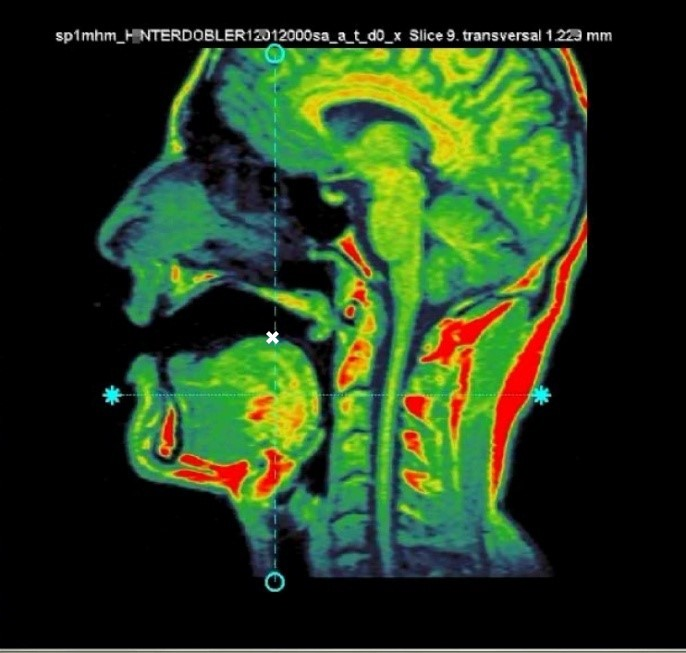
\includegraphics[width=\textwidth]{figures/mrt_a_Kreuz.jpg}
         \caption{[a]}
         \label{fig:Vokaltrakt_a}
     \end{subfigure}
     \hfill
     \begin{subfigure}[b]{0.3\textwidth}
         \centering
         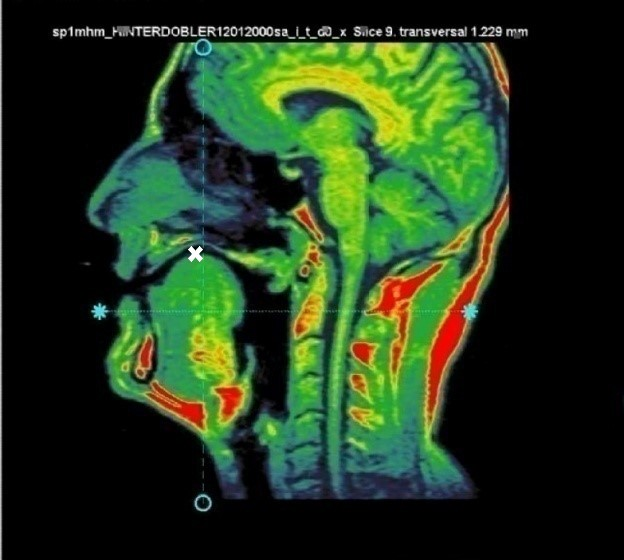
\includegraphics[width=\textwidth]{figures/mrt_i_Kreuz.jpg}
         \caption{[i]}
         \label{fig:Vokaltrakt_i}
     \end{subfigure}
     \hfill
     \begin{subfigure}[b]{0.32\textwidth}
         \centering
         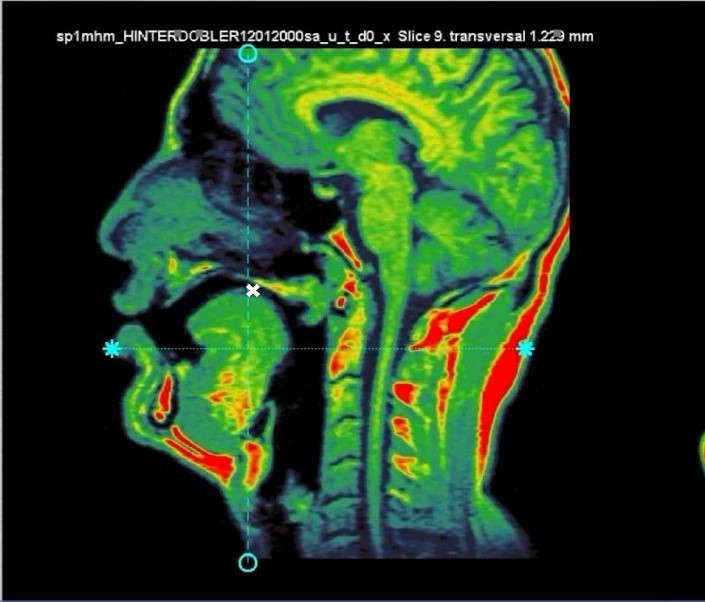
\includegraphics[width=\textwidth]{figures/mrt_u_Kreuz.jpg}
         \caption{[u]}
         \label{fig:Vokaltrakt_u}
     \end{subfigure}
        \caption{Vokaltraktkonfigurationen bei unterschiedlichen Vokalen (MRT-Aufnahmen, Quelle: Phil Hoole, Institut für Phonetik und Sprachverarbeitung, Ludwig-Maximilians-Universität München). Die weißen Kreuze wurden später hinzugefügt und markieren jeweils den höchsten Punkt des Zungenrückens.}
        \label{fig:dreiVokale}
\end{figure}

Man kann erkennen, dass die Zunge bei jedem Vokal eine andere Form annimmt. Bei \textipa{[a]} liegt sie relativ flach im Mund, bei \textipa{[i]} bildet sie im palatalen Bereich eine Verengung und bei \textipa{[u]} im velaren Bereich. Diese Unterschiede werden in der Phonetik als Unterschiede in der \is{Zungenhöhe}Zungenhöhe und der \is{Zungenlage}Zungenlage beschrieben. Der Referenzpunkt bei der Ermittlung der Zungenhöhe und Zungenlage ist der \textit{höchste Punkt des Zungenrückens}\is{Zungenrücken}, der als weißes Kreuz in den Abbildungen markiert ist. 

Die \is{Zungenhöhe}Zungenhöhe von \textipa{[a]} ist, verglichen mit den anderen beiden Lauten, \textit{tief}: Die Zunge liegt flach im Mund und das weiße Kreuz ist deutlich tiefer als bei \textipa{[i]} und \textipa{[u]}. Die Zungenhöhe von \textipa{[i]} und \textipa{[u]} ist, verglichen mit \textipa{[a]}, \textit{hoch}. Die \is{Zungenlage}Zungenlage von \textipa{[i]} ist \textit{vorn} (Vorderzungenvokal), denn das weiße Kreuz ist, verglichen mit \textipa{[u]}, relativ weit vorne. Die Zungenlage von \textipa{[u]} ist \textit{hinten} (Hinterzungenvokal). \textipa{[a]} ist im Deutschen von der Zungenlage her ein zentraler Vokal, die Zungenlage variiert abhängig von Kontext und Sprecher(in) sehr stark um die Mitte (\cite[14]{Becker1998}, \cite[225]{PaetzoldSimpson1997}, \cite[57]{Brunner2009}).

\subsection{Zungenhöhe und Zungenlage}

Zungenhöhe und Zungenlage eines Lautes können im \textit{Vokalviereck}\is{Vokalviereck} (auch: \textit{Vokaltrapez, Vokaldreieck}) dargestellt werden (vgl. Abbildung~\ref{fig:Vokalviereck}). Das Vokalviereck bezieht sich auf die Mittsagittale, also die Ebene, die den Kopf in eine gleich große rechte und linke Hälfte teilt. Auf dieser Ebene gibt das Vokalviereck an, ob Vokale im Vergleich zu anderen Vokalen weiter vorn, weiter hinten, weiter oben oder weiter unten gebildet werden.

Da man nicht die gesamte Kontur der Zunge auf einen Punkt reduzieren kann, bezieht sich die Darstellung auf den höchsten Punkt des Zungenrückens bei der Produktion des jeweiligen Vokals. Die weißen Kreuze in Abbildung~\ref{fig:dreiVokale} sind also die Referenzpunkte, die im Vokalviereck dargestellt werden.

\begin{figure}
    \centering
    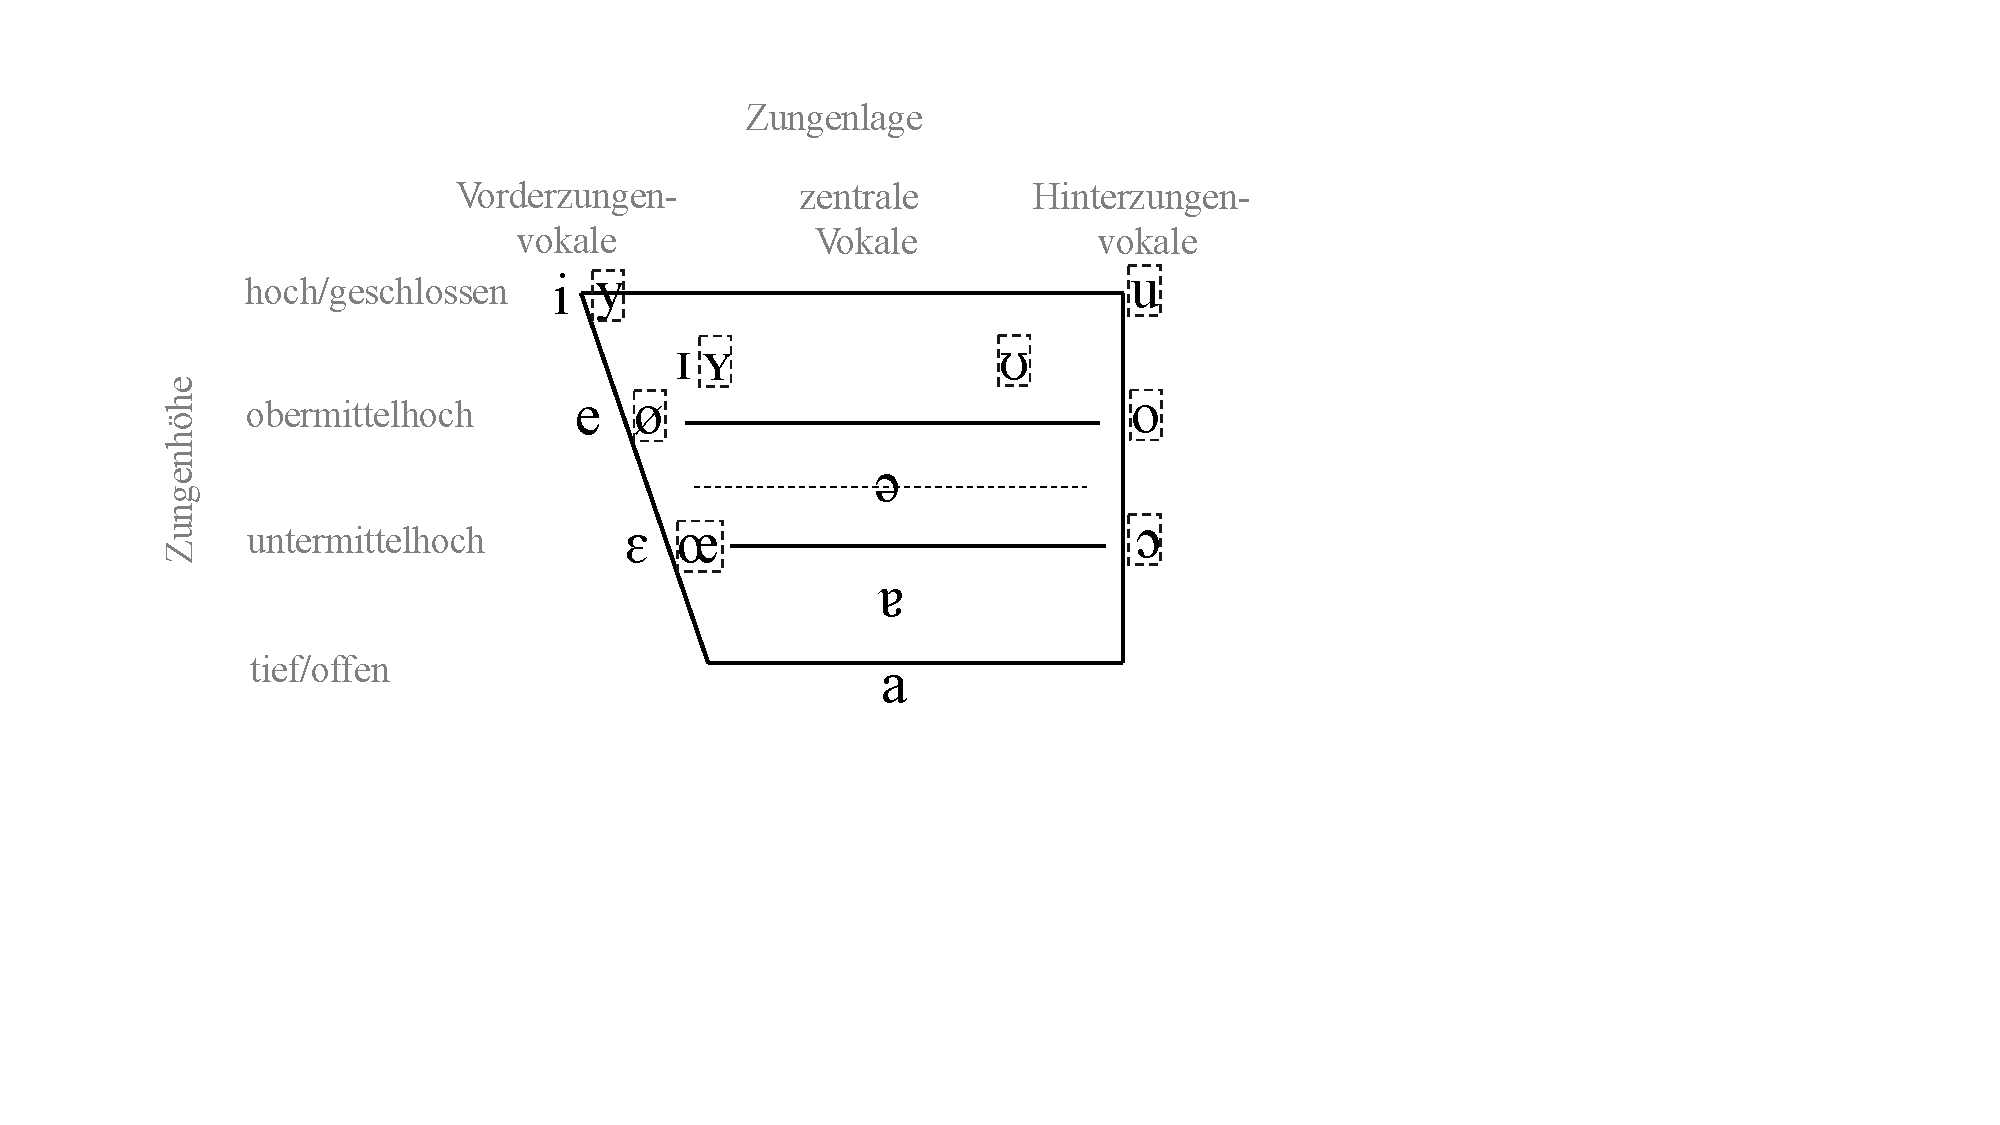
\includegraphics[width=1\textwidth]{figures/Vokalviereck.pdf}
    \caption{Vokalviereck mit den deutschen Vokalen. Gerundete Vokale sind durch ein gestricheltes Kästchen markiert.\label{fig:Vokalviereck}}
\end{figure}

Im Vokalviereck\is{Zungenlage}\is{Vokalviereck}\is{Vorderzungenvokale}\is{Hinterzungenvokal} entspricht die horizontale Dimension der Zungenlage. Ein Laut kann vorn, in der Mitte oder hinten gebildet werden. Die vertikale Dimension entspricht der Zungenhöhe. Ein Laut kann hoch, obermittelhoch, untermittelhoch oder tief sein. Links stehen die Vokale, bei denen die Zunge vorne im palatalen Bereich ist. Diese Vokale werden \textit{Vorderzungenvokale} genannt. Rechts stehen die Vokale, bei denen die Zunge hinten im velaren Bereich ist. Diese Vokale werden \textit{Hinterzungenvokale} genannt. Die Vokale zwischen Vorder- und Hinterzungenvokalen nennt man \textit{zentrale Vokale}.\footnote{Im internationalen phonetischen Alphabet gibt es für die tiefen Vokale das Zeichen \textipa{[a]} für den Vorderzungenvokal und \textipa{[A]} für den Hinterzungenvokal (etwa in Englisch \textit{bath}). Das deutsche \textipa{[a]} in \textit{Bahn} oder \textit{Bann} wird eigentlich zwischen diesen beiden Lauten verortet. Es gibt deshalb phonetisch gesehen keinen guten Grund dafür, das Symbol \textipa{[a]} zu verwenden. Im Gegenteil, phonologisch gesehen, sollte man eher \textipa{[A]} transkribieren, da sich der Laut phonologisch wie ein Hinterzungenvokal verhält. Beispielsweise wird <ch> nach Vorderzungenvokalen \textipa{[\c{c}]} gesprochen, nach \textipa{[a]} aber \textipa{[\textchi ]} \citep[14]{Becker1998}. Dass wir das Symbol \textipa{[a]} verwenden ist also nicht gut begründet, folgt aber den meisten anderen Einführungswerken.}

Um sich die artikulatorischen Unterschiede zu verdeutlichen, kann man versuchen, einen Vorderzungenvokal und einen Hinterzungenvokal ohne Pause nacheinander zu sprechen. Wir wählen den Vorderzungenvokal \textipa{[y]},\footnote{Wir wählen hier \textipa{[y]} statt \textipa{[i]}, weil \textipa{[y]} dieselbe Lippenkonfiguration wie \textipa{[u]} hat und deshalb besser mit \textipa{[u]} verglichen werden kann.} wie im Anlaut von \textit{Übung}, und den Hinterzungenvokal \textipa{[u]}, wie im Anlaut von \textit{Uhu}, und sprechen \textipa{[yyyuuu]}. Dabei kann man beobachten, dass die Zunge am Gaumen von vorn nach hinten gleitet.

Vokale\is{Zungenhöhe}, bei denen die Zunge im Vergleich zu anderen Vokalen relativ hoch liegt, nennt man \textit{hohe Vokale}. In einigen Lehrbüchern findet man auch den Begriff \textit{geschlossene Vokale}. Vokale, bei denen die Zunge sehr weit unten liegt, nennt man \textit{tiefe Vokale} (auch: \textit{offene Vokale}). In der Abbildung sind noch zwei weitere Ebenen eingezeichnet: die \textit{obermittelhohen} und die \textit{untermittelhohen Vokale}. Diese vier Ebenen werden im Folgenden genauer beschrieben.

Wenn man die beiden Vokale \textipa{[i]} und \textipa{[a]} so nacheinander spricht, dass sie ineinander übergehen, kann man feststellen, dass die Zunge -- meist zusammen mit dem Kiefer -- nach unten wandert. Man kan die Vokale \textipa{[i]} wie in \textit{D\underline{ie}b} \textipa{[di:p]}, \textipa{[e]} wie in \textit{\underline{e}ben} \textipa{[\textprimstress Pe:.b@n]}, \textipa{[E]} wie in \textit{B\underline{e}tt} \textipa{[bEt]} und \textipa{[a]} wie in \textit{h\underline{a}ben} \textipa{[\textprimstress ha:.b@n]} oder \textipa{[\textprimstress ha:.b\s{m}]} nacheinander sprechen, sodass ein Vokal in den anderen übergeht: \textipa{[ieEa]}. Dabei bewegt sich die Zunge zusammen mit dem Kiefer nach unten, aber diesmal in vier Schritten. Diese vier Schritte entsprechen den vier Ebenen im Vokalviereck: hoch, obermittelhoch, untermittelhoch, tief.

Dasselbe Experiment kann man für die Hinterzungenvokale machen. Wenn man die Vokale \textipa{[u]} wie in \textit{Hut} \textipa{[hu:t]}, \textipa{[o]} wie in \textit{Mond} \textipa{[mo:nt]}, \textipa{[O]} wie in \textit{oft} \textipa{[POft]} und \textipa{[a]} nacheinander spricht, so dass ein Vokal in den anderen übergeht -- \textipa{[uoOa]} -- wird man feststellen, dass Kiefer und Zunge abgesenkt werden.

Um die anderen Vokale im Vokalviereck beschreiben zu können, braucht man weitere Beschreibungsparameter. 

\subsection{Lippenrundung}
\is{Lippenrundung}
Auffällig ist in Abbildung~\ref{fig:dreiVokale} neben den Unterschieden in der Zungenposition, dass die Lippenkonfiguration zwischen \textipa{[a, i]} und \textipa{[u]} sehr unterschiedlich ist. Bei \textipa{[u]} werden die Lippen nach vorne gestülpt (wie für einen Kuss). Vokale, die mit vorgestülpten Lippen produziert werden, bezeichnet man als \textit{gerundete Vokale}\is{gerundet}. Bei \textipa{[a]} und \textipa{[i]} sind die Lippen nicht gerundet. Solche Vokale bezeichnet man als \textit{ungerundete Vokale}\is{ungerundet}. 

Einige Vokale haben in etwa dieselbe Zungenhöhe und Zungenlage, unterscheiden sich aber in der Lippenrundung. Wenn man den Vokal \textipa{[i]} lange aushält und dann die Lippen rundet, ohne die Zunge zu bewegen, erhält man den Vokal \textipa{[y]} wie in \textit{bügeln} \textipa{[\textprimstress by:.g@ln]}. Wenn man dasselbe mit \textipa{[e]} probiert, erhält man den Vokal \textipa{[\o]}, wie in \textit{Möbel} \textipa{[\textprimstress m\o :.b@l]}. Aus \textipa{[E]}, dem Laut in \textit{Bett}, wird mit Lippenrundung \textipa{[\oe]}, der erste Vokal in \textit{öfter} \textipa{[\textprimstress P\oe f.t5]}.


\subsection{Gespanntheit}
\label{subsection:Gespanntheit}
\is{Gespanntheit}
Der Parameter \textit{Gespanntheit} steht in Relation zur Vokallänge. Die Unterscheidung von \is{Langvokal}\is{Kurzvokal} sogenannten \textit{Lang-} und \textit{Kurzvokalen} spielt im Orthografieerwerb eine wichtige Rolle, denn es gibt spezielle orthografische Markierungen für die beiden Klassen von Lauten. So steht nach einem Kurzvokal häufig (aber längst nicht immer) ein Doppelkonsonant, etwa in \textit{doppelt, Mitte, Rinne}. Ein Langvokal kann durch <ie>, ein stummes h oder einen Doppelvokal gekennzeichnet werden: \textit{schief, Mehl, Saal}. Tabelle~\ref{tab:LangKurzvokale} stellt die beiden Lautklassen gegenüber. \is{Transkription!Längenzeichen}Die Doppelpunkte in den Transkriptionen stehen für die Länge der Langvokale.

\begin{table}
    \centering
        \caption{\label{tab:LangKurzvokale} \gqq{Langvokale} und \gqq{Kurzvokale} im Deutschen mit Beispielwörtern}
    \begin{tabular}{llll}\lsptoprule
         \multicolumn{2}{c}{\gqq{Langvokale}} &\multicolumn{2}{c}{\gqq{Kurzvokale}} \\\midrule
        \textipa{[i:]} & \textit{pieken} \textipa{[\textprimstress pi:.k@n]} & \textipa{[I]}&  \textit{picken} \textipa{[\textprimstress pI\.*{k}@n]}\\
                \textipa{[e:]} & \textit{beten} \textipa{[\textprimstress be:.t@n]} & \textipa{[E]}&  \textit{Betten} \textipa{[\textprimstress bE\.*{t}@n]}\\
                \textipa{[u:]} & \textit{Ruhm} \textipa{[Ku:m]} & \textipa{[U]}&  \textit{Rum} \textipa{[KUm]}\\
                \textipa{[o:]} & \textit{Ofen} \textipa{[\textprimstress Po:.f@n]} & \textipa{[O]}&  \textit{offen} \textipa{[\textprimstress PO\.*{f}@n]}\\
                \textipa{[a:]} & \textit{Bahn} \textipa{[ba:n]} & \textipa{[a]}&  \textit{Bann} \textipa{[ban]}\\
                        \textipa{[y:]} & \textit{Hüte} \textipa{[\textprimstress hy:.t@]} & \textipa{[Y]}&  \textit{Hütte} \textipa{[\textprimstress hY\.*{t}@]}\\
                                \textipa{[\o :]} & \textit{Höhle} \textipa{[\textprimstress h\o :.l@]} & \textipa{[\oe]}&  \textit{Hölle} \textipa{[\textprimstress h\oe \.*{l}@]}\\
        \lspbottomrule
    \end{tabular}
\end{table}



Wenn man die Wörter in Tabelle~\ref{tab:LangKurzvokale} mit gleicher Sprechgeschwindigkeit sprechen und mit einem Mikrophon aufnehmen würde, würde man feststellen, dass die Vokale in den Wörtern in der linken Spalte (die Langvokale), tatsächlich länger sind als die entsprechenden Vokale in den Wörtern in der rechten Spalte (die Kurzvokale). Diese Unterschiede bezeichnet man auch als Unterschiede in der \textit{Vokalquantität}\is{Vokalquantität}.

Die Begriffe Lang- und Kurzvokal sind gut etabliert. \citet{Iivonen1987} und \citet{Spiekermann2002} zeigen, dass der Längenkontrast in Österreich und Süddeutschland auch tatsächlich das hauptsächliche Unterscheidungsmerkmal zwischen den Lautklassen darstellt. In Nord- und Mitteldeutschland beschreibt der Längenunterschied den Kontrast zwischen den beiden Lautklassen aber nur unzureichend. 

Schaut man ins Vokalviereck in Abbildung~\ref{fig:Vokalviereck}, welches sich am norddeutsch geprägten Standard orientiert, stellt man fest, dass die Vokalpaare sich nicht nur durch die Länge, sondern vor allem durch die Zungenposition (Zungenhöhe und Zungenlage) unterscheiden. Diese Unterschiede bezeichnet man auch als Unterschiede in der \textit{Vokalqualität}\is{Vokalqualität}. Der Vokal \textipa{[i]} in \textit{pieken} wird mit höherer Zungenposition und weiter vorne gebildet als der Vokal \textipa{[I]} in \textit{picken}. Der Vokal \textipa{[I]} ist sogar näher am \textipa{[e]} als am \textipa{[i]}. Die Ähnlichkeit zum \textipa{[e]} kann man als Sprecher(in) des norddeutschen Standards auditiv erfahrbar machen, wenn man \textit{picken} langsam vor sich hin spricht, sodass der Vokal gedehnt wird: \mbox{\textit{pi-- --cken}}. Das \textit{pi----} klingt jetzt dem \textit{Pe} in \textit{Pegel} deutlich ähnlicher als dem \textit{pie} in \textit{pieken}. Eigentlich ist das \textipa{[I]} also eher ein gekürztes \textipa{[e]} als ein gekürztes \textipa{[i]}. Deshalb findet man bei Erstklässlern im nordeutschen Raum auch häufig eine Verwechslung von <i> und <e>, etwa <mech> für \textit{mich}.

Das kurze \textipa{[U]} ist artikulatorisch und auditiv näher am langen \textipa{[o:]} als am langen \textipa{[u:]}. Wenn norddeutsche Sprecher \textit{Rum} sehr gedehnt sprechen, hören wir eher \textit{Rom} als \textit{Ruhm}. Dass es Kindern genauso geht, zeigen Schreibungen wie <*mont> für \textit{Mund}, eine Schreibung, die wir schon am Anfang des Kapitels betrachtet haben.

Auch die Schreibung <*höte> für \textit{Hütte} ist in der genannten Varietät darauf zurückzuführen, dass die Lang- und Kurzvokale sich artikulatorisch und akustisch deutlich unterscheiden. Wenn man das \textipa{[Y]} in \textit{Hütte} gedehnt spricht, klingt der Laut eher wie das \textipa{[\o :]} in \textit{Höfe}, aber nicht wie das \textipa{[y:]} in \textit{Hüte}. Das liegt daran, dass die Zunge bei \textipa{[Y]} tiefer als bei \textipa{[y]} liegt.

Die sogenannten Lang- und Kurzvokale unterscheiden sich also in der Länge, aber auch in der Zungenposition, weshalb die Begriffe Lang- und Kurzvokale den Unterschied zumindest für den hier beschriebenen Standard nicht gut erfassen. In der phonetischen Literatur wird der Unterschied deshalb häufig \textit{Gespanntheitsopposition}\is{Gespanntheit} genannt. Die Langvokale werden als \textit{gespannte Vokale} und die Kurzvokale als \textit{ungespannte Vokale} bezeichnet (\zB \cite[39--47]{Becker1998}, \cite[227]{Pompino-Marschall2020}, \cite[26]{FuhrhopPeters2013}, \cite[27]{Hall2000}). Diese Begriffe haben ihren Ursprung in der Annahme, dass für die gespannten Vokale die Zungenmuskeln stärker gespannt sein müssen, weil diese Vokale an extremeren Positionen im Mund gebildet werden (sie stehen weiter außen im Vokalviereck als die ungespannten Partner). Experimentelle Messungen bestätigen das nicht eindeutig, der Begriff Gespanntheit hält sich jedoch \citep[43--44]{Becker1998}. Wir werden die Vokale in der linken Spalte in Tabelle~\ref{tab:LangKurzvokale} deshalb als gespannte Vokale bezeichnen und die in der rechten Spalte als ungespannte Vokale.

Bisher scheint der Unterschied vielleicht vor allem ein terminologischer zu sein: Gespannte Vokale sind nach der bisherigen Diskussion offenbar lange Vokale. Es ist jedoch wichtig, zu verstehen, dass es sich bei vokalischen Kontrasten wie dem zwischen \textit{bieten} und \textit{bitten} zumindest in Nord- und Mitteldeutschland nicht um einen reinen Längenkontrast handelt. Es spricht aber nichts gegen die Verwendung der Termini Lang- und Kurzvokal im Unterricht. \citet[204--207]{Spiekermann2002} zeigt, dass Kinder, die den Kontrast dialektbedingt tatsächlich nur als Längenkontrast produzieren, trotz der Terminologie keinen Vorteil gegenüber Kindern mit eher norddeutscher Aussprache haben.

Anders als die bisherigen Beispiele suggerieren, kann man allerdings von der Gespanntheit eines Vokals nicht sicher auf die Länge des Vokals schließen. Die Vokale, die bisher diskutiert wurden (Tabelle~\ref{tab:LangKurzvokale}), treten alle in betonten Silben auf. Für diese Position kann man tatsächlich sagen, dass die gespannten Vokale lang und die ungespannten kurz sind. In unbetonter Position sind die Verhältnisse anders. Dazu vergleichen wir den ersten Vokal in den Wörtern \textit{leben} und \textit{lebendig}. In beiden Fällen handelt es sich um den gespannten Vokal \textipa{[e]}. Das \textipa{[e]} in \textit{leben} ist aber länger als das \textipa{[e]} in \textit{lebendig}. Das liegt daran, dass \textit{leben} auf der ersten Silbe betont ist, \textit{lebendig} aber auf der zweiten. In betonter Position werden gespannte Vokale also gelängt. Man transkribiert deshalb \textit{leben} \textipa{[\textprimstress le:.b@n]} mit einem Doppelpunkt\is{Transkription!Längenzeichen}, der die Länge signalisiert, und \textit{lebendig} \textipa{[le\textprimstress bEn.dI\c{c}]} oder \textipa{[le\textprimstress bEn.dIk]} ohne Doppelpunkt.

Gespannte Vokale sind also nicht immer lang, sondern sie sind nur in betonter Position lang. Deshalb ist der Terminus Langvokal für diese Vokale nicht immer zutreffend.

Bei den ungespannten Vokalen gibt es keinen deutlichen Längenunterschied zwischen betonten und unbetonten Vokalen. Dazu vergleichen wir das \textipa{[E]} in \textit{Bäcker} und \textit{Bäckerei}. \textit{Bäcker} ist auf der ersten Silbe betont, aber das \textipa{[E]} ist kurz. \textit{Bäckerei} ist auf der letzten Silbe betont, und das \textipa{[E]} ist kurz. Man transkribiert deshalb: \textipa{[\textprimstress bE\.*k5]} und \textipa{[bE\.*k@\textprimstress K\t*{aI}]}.

Man kann also drei Gruppen von Vokalen unterscheiden \citep[120--121]{Jessen2010}: 
\begin{itemize}
    \item die gespannten langen Vokale
    \item die gespannten kurzen Vokale
    \item die ungespannten Vokale
\end{itemize}

Tabelle~\ref{tab:GespanntUngespannt} besteht deshalb im Gegensatz zu Tabelle~\ref{tab:LangKurzvokale} aus drei Spalten, nämlich den beiden äußeren, die wir aus Tabelle~\ref{tab:LangKurzvokale} kennen, und einer neuen mittleren Spalte für die gespannten Vokale in unbetonten Silben.

\begin{table}
    \centering
%\resizebox{\textwidth}{!}{
\oneline{
    \begin{tabular}{llllll}\lsptoprule
         \multicolumn{2}{c}{gespannte lange Vokale} & \multicolumn{2}{c}{gespannte kurze Vokale} &\multicolumn{2}{c}{ungespannte Vokale} \\\midrule
        \textipa{[i:]} & \textit{pieken} \textipa{[\textprimstress pi:.k@n]} &\textipa{[i]} & \textit{Zitrone} \textipa{[\t{ts}i\textprimstress tKo:.n@]}  & \textipa{[I]}&  \textit{picken} \textipa{[\textprimstress pI\.*k@n]}\\
                \textipa{[e:]} & \textit{beten} \textipa{[\textprimstress be:.t@n]} &\textipa{[e]} & \textit{lebendig} \textipa{[le\textprimstress bEn.dI\c{c}]} & \textipa{[E]}&  \textit{Betten} \textipa{[\textprimstress bE\.*t@n]}\\
                \textipa{[u:]} & \textit{Ruhm} \textipa{[Ku:m]} & \textipa{[u]}& \textit{Museum} \textipa{[mu\textprimstress ze:.Um]} &\textipa{[U]} &  \textit{Rum} \textipa{[KUm]}\\
                \textipa{[o:]} & \textit{Ofen} \textipa{[\textprimstress Po:.f@n]} &\textipa{[o]} & \textit{Modell} \textipa{[mo\textprimstress dEl]} & \textipa{[O]}&  \textit{offen} \textipa{[\textprimstress PO\.*f@n]}\\
                        \textipa{[y:]} & \textit{Hüte} \textipa{[\textprimstress hy:.t@]} &\textipa{[y]} & \textit{Myom} \textipa{[my\textprimstress o:m]} & \textipa{[Y]}&  \textit{Hütte} \textipa{[\textprimstress hY\.*t@]}\\
                                \textipa{[\o :]} & \textit{Höhle} \textipa{[\textprimstress h\o :.l@]} &\textipa{[\o ]} & \textit{Ödem} \textipa{[P\o \textprimstress de:m]} & \textipa{[\oe]}&  \textit{Hölle} \textipa{[\textprimstress h\oe \.*l@]}\\
                                \cmidrule(r){1-4}\cmidrule(l){5-6}
          \multicolumn{4}{c}{peripher} &  \multicolumn{2}{c}{zentral}\\
        \cmidrule(r){1-2}\cmidrule(l){3-6}
            \multicolumn{2}{c}{lang} &  \multicolumn{4}{c}{kurz}\\\lspbottomrule
    \end{tabular}
    }
 \caption{Einteilung der deutschen Vokale in gespannt/ungespannt und lang/kurz}
        \label{tab:GespanntUngespannt}
\end{table}

Die Vokale in der linken und mittleren Spalte sind gespannt und haben also eine \textit{periphere} (extremere) Zungenposition. Sie werden mit demselben Symbol transkribiert, da die Zungenposition vergleichbar ist. Die Vokale in der rechten Spalte haben eine \textit{zentralere} Zungenposition (eher mittig). Sie werden deshalb mit einem anderen Symbol transkribiert. Die Vokale in der linken Spalte sind lang und werden deshalb \is{Transkription!Längenzeichen}mit Doppelpunkt transkribiert. Die Vokale in den beiden anderen Spalten sind kurz und werden deshalb ohne Doppelpunkt transkribiert.

Es ist auffällig, dass native Wörter vor allem in der linken und rechten Spalte zu finden sind. Typischerweise kommen gespannte Vokale vor allem in betonten Silben vor. In die mittlere Kategorie fallen vor allem Fremdwörter. Es ist wichtig, diese Kategorie identifizieren zu können, da bei diesen Wörtern die deutschen Orthografieregeln für die gespannten Vokale nicht angewandt werden können. Beispielsweise gibt es bei diesen Wörtern kein <ie> und auch kein Dehnungs-\textit{h}. Kindliche Schreibungen wie <*Zietrone> oder <*Tehater>, bei denen die Regeln für die gespannten Langvokale angewandt werden, sind darauf zurückzuführen, dass die Kinder die Vokale als gespannt wahrnehmen.

Zwischen den Vokalen \textipa{[a]} in \textit{Bann} und \textipa{[a:]} in \textit{Bahn} gibt es laut \citet[14--15]{Becker1998} einen messbaren, aber keinen hörbaren Unterschied in der Vokalqualität. Sie unterscheiden sich also nur in der Vokalquantität und sind deshalb in Tabelle~\ref{tab:GespanntUngespannt} nicht enthalten.


Vor allem in der Bildungssprache\footnote{Unter Bildungssprache verstehen wir hier \citet[]{Habermas1977} folgend ein sprachliches Register, welches in Bildungsinstitutionen verwendet wird und welches allgemein zur Bildungsaneignung verwendet wird.} wird \citet[15--16]{Becker1998} zufolge häufig ein Unterschied zwischen \textipa{[E:]}, wie in \textit{Dänen}, und \textipa{[e:]}, wie in \textit{dehnen}, gemacht. Außerhalb von Bildungskontexten ist diese Unterscheidung in Nord- und Ostdeutschland und in Ostösterreich laut \citet[67]{DudenAussprache2023} jedoch kaum zu hören, beide Wörter werden \textipa{[\textprimstress de:n@n]} oder \textipa{[\textprimstress de:n\s{n}]} gesprochen. Auch in anderen deutschsprachigen Gebieten fallen die beiden Laute bei vielen Sprechern zusammen. Lediglich in der Schweiz wird konsequent zwischen \textipa{[E:]} und \textipa{[e:]} unterschieden \citep[67]{DudenAussprache2023}. Laut Ausspracheduden sind beide Varianten standardgemäß, das \citet[138]{DudenZweifelsfaelle2021} empfiehlt die Aussprache \textipa{[E:]}, \zB in \textit{Träne} \textipa{[\textprimstress tKE:.n@]} statt \textipa{[\textprimstress tKe:.n@]}.

\largerpage
  In (\ref{väter}) bis (\ref{gewähren}) sind weitere Beispiele gegeben, bei denen es eine Diskrepanz zwischen dem gibt, was laut \citet{DudenZweifelsfaelle2021} empfohlen wird (erste Transkription bei jedem Beispiel) und der Lautung, die in weiten Teilen Deutschlands und Österreichs produziert wird (zweite Transkription). 
\ea
\ea \label{väter}Väter: \textipa{[\textprimstress fE:.t5]} vs. \textipa{[\textprimstress fe:.t5]}
\ex \label{mädchen}Mädchen: \textipa{[\textprimstress mE:t.\c{c}@n]} vs. \textipa{[\textprimstress me:t.\c{c}@n]}
\ex \label{ähnlich}ähnlich: \textipa{[\textprimstress PE:n.lI\c{c}]} vs. \textipa{[\textprimstress Pe:n.lI\c{c}]}
\ex \label{käse}Käse: \textipa{[\textprimstress kE:.z@]} vs. \textipa{[\textprimstress ke:.z@]}
\ex \label{gewähren}gewähren: \textipa{[g@\textprimstress vE:.K@n]} vs. \textipa{[g@\textprimstress ve:.K@n]}
\z
\z

\citet[14--15 und Quellen darin]{Becker1998} zufolge hat die \textipa{[E:]}-Aussprache ihren Ursprung in der Schriftsprache, wo zwischen <e> und <ä> unterschieden wird. Die einzigen Fälle, in denen viele Sprecherinnen und Sprecher tatsächlich häufig \textipa{[E:]} sprechen, sind Wörter, deren Aussprache sonst mit der anderer Wörter zusammenfallen würde, etwa \textit{sehen--sähen, geben--gäben} und das zuvor erwähnte \textit{dehnen--Dänen}.


\subsection{Reduktionsvokale}\label{subsection:Reduktionsvokale}

Alle Vokale, die bisher diskutiert wurden, können den Nukleus einer betonten Silbe bilden. Es gibt jedoch auch Vokale, die das nicht können. Diese Vokale nennt man \textit{Reduktionsvokale}. Im Deutschen gibt es zwei Reduktionsvokale, den \textit{Schwa-Laut} \textipa{[@]} und das \textit{tiefe Schwa} \textipa{[5]}, auch \textit{a-Schwa} oder \textit{Lehrer-Schwa} genannt. 

Das Schwa \is{Laute!Schwa} \textipa{[@]} wird orthografisch <e> geschrieben und kommt im Standarddeutschen nur in unbetonten Silben vor, wie in den Beispielen (\ref{ex:Lage}) und (\ref{ex:geteilt}). Im Vokalviereck steht der Schwa-Laut direkt im Zentrum (vgl. Abbildung \ref{fig:Vokalviereck}). Er wird gebildet, indem die Zunge entspannt im Mund liegt.

\ea
\ea \label{ex:Lage} Lage \textipa{[\textprimstress la:.g@]}
\ex \label{ex:geteilt} geteilt \textipa{[g@\textprimstress t\t*{aI}lt]}
\z 
\z

Im Standarddeutschen kommt er außerdem in förmlicher Rede in der Infinitivendung der Verben vor, wie in Beispiel (\ref{ex:lesen}), aber auch in vielen anderen Endsilben, wie in Beispiel (\ref{ex:Mantel}). An diesen Stellen wird er in fließender Rede jedoch oft getilgt (sogenannte Schwa-Tilgung, vgl. Abschnitt~\ref{sec:Schwatilgung}).

\ea
\ea \label{ex:lesen} \textit{lesen}, explizit: \textipa{[\textprimstress le:.z@n]}, in fließender Rede: \textipa{[\textprimstress le:.z\s{n}]}
\ex \label{ex:Mantel} \textit{Mantel}, explizit: \textipa{[\textprimstress man.t@l]}, in fließender Rede: \textipa{[\textprimstress man.t\s{l}]}\footnote{Ein Strichlein unter einem Konsonanten bedeutet, dass der Konsonant silbisch ist. Er übernimmt also die Nukleus-Funktion, die sonst von einem Vokal wahrgenommen wird.}
\z 
\z


Das \is{Laute!tiefes Schwa} tiefe Schwa \textipa{[5]} wird <r> oder <er> geschrieben. Wenn es zusammen mit einem anderen Vokal den Nukleus bildet, wie in Bespiel (\ref{ex:für}), wird es <r> geschrieben. Wenn es alleine den Nukleus bildet, wie in den Beispielen (\ref{ex:Drucker}) und (\ref{ex:verbinden}) wird es <er> geschrieben. 

\ea
\ea \label{ex:für} für \textipa{[fy5]} 
\ex \label{ex:Drucker} Drucker \textipa{[\textprimstress drU\.*k5]}
\ex \label{ex:verbinden} verbinden \textipa{[f5\textprimstress bIn.d@n]}
\z 
\z

Das tiefe Schwa \textipa{[5]} und das Schwa \textipa{[@]} sind bedeutungsunterscheidend, wie die Beispiele (\ref{ex:Lehre-Lehrer}) und (\ref{ex:meiste-Meister}) zeigen.\footnote{Solche Beispiele, die sich nur durch einen einzigen Laut unterscheiden, nennt man Minimalpaare (vgl. Abschnitt~\ref{sec:Allophone}.)}

\ea
\ea \label{ex:Lehre-Lehrer} Lehre -- Lehrer \textipa{[\textprimstress le:.K@} -- \textipa{\textprimstress le:.K5]}
\ex \label{ex:meiste-Meister} meiste -- Meister \textipa{[\textprimstress m\t*{aI}s.t@} -- \textipa{\textprimstress m\t*{aI}s.t5]}
\z 
\z


Im Vokalviereck steht das tiefe Schwa zwischen Schwa und \textipa{[a]} (vgl. Abbildung \ref{fig:Vokalviereck} auf Seite \pageref{fig:Vokalviereck}). Akustisch ist es dem \textipa{[a]} sehr ähnlich, weshalb man bei Schreibanfängern häufig a-Schreibungen findet: <*füa> (\textit{für}), <*Kinda> (\textit{Kinder}). \citet[42]{RathckeMooshammer2020} zeigen, dass Minimalpaare wie in den Beispielen (\ref{ex:Cola}), (\ref{ex:Feta}) und (\ref{ex:Opa}) in den nördlichen Regionen Deutschlands nicht unterscheidbar produziert werden. 

\ea
\ea \label{ex:Cola} Cola \textipa{[\textprimstress ko:.la]} vs. Kohler \textipa{[\textprimstress ko:.l5]}
\ex \label{ex:Feta} Feta \textipa{[\textprimstress fe:.ta]} vs. Väter \textipa{[\textprimstress fe:.t5]}
\ex \label{ex:Opa} Opa \textipa{[\textprimstress Po:.pa]} vs. Oper \textipa{[\textprimstress Po:.p5]} 
\z 
\z


Wenn, wie in Beispiel (\ref{ex:für}), das tiefe Schwa zusammen mit einem anderen Vokal in einer Silbe steht, bildet es mit diesem Vokal zusammen einen \is{Diphthong}Diphthong (vgl. Abschnitt~\ref{subsec:Diphthonge}). 

Vor allem nach ungespannten Vokalen kann statt des tiefen Schwas ein r-Laut gesprochen werden. Das kann man etwa bei der Aussprache von \textit{Erde} beobachten \citep[308]{DudenAussprache2023}. In Dialektregionen, wo der Vokal gespannt gesprochen wird, wird das tiefe Schwa bevorzugt: \textipa{[\textprimstress Pe:5.d@]}, wenn der Vokal  ungespannt gesprochen wird, folgt ihm eher ein r-Laut: \textipa{[\textprimstress PEr.d@]}.

\subsection{Diphthonge}
\label{subsec:Diphthonge}
\largerpage
Vokale können in \textit{Monophthonge}\is{Monophthong} und \textit{Diphthonge}\is{Diphthong} eingeteilt werden. Alle Vokale, die bisher besprochen wurden, \zB \textipa{[i, a, u]}, sind Monophthonge. Bei Monophthongen bewegt sich die Zunge in eine bestimmte vokalische Position und dann bewegt sie sich zum Koda-Konsonanten oder einem Laut in der nächsten Silbe.

Diphthonge (auch \textit{Zwielaute}\is{Diphthong!Zwielaut} genannt) sind einsilbige Verbindungen aus zwei vokalischen Segmenten, also zwei Segmenten, die zusammen einen Nukleus bilden, \zB \textipa{[\t*{aU}]}. In Tabelle~\ref{tab:EinsilbigZweisilbig} sind zweisilbige und einsilbige Vokalkombinationen gegenübergestellt. \textit{Lea} ist ein zweisilbiges Wort, \textipa{[e]} und \textipa{[a]} gehören zu zwei unterschiedlichen Silben und sind daher Monophthonge. \textit{leer} ist akustisch sehr ähnlich, aber einsilbig, da das Wort den Diphthong \textipa{[\t*{e5}]} enthält. \textipa{[e]} und \textipa{[5]} gehören zur selben Silbe. 

\begin{table}
    \centering
        \caption{\label{tab:EinsilbigZweisilbig} Zweisilbige (erste Spalte) und einsilbige (zweite Spalte) Vokalverbindungen.}
    \begin{tabular}{ll}\lsptoprule
        zweisilbig & einsilbig \\\midrule
        \textit{Lea} \textipa{[\textprimstress le:.a]}& \textit{leer} \textipa{[l\t*{e5}]}\\
        \textit{Pia} \textipa{[\textprimstress pi:.a]}& \textit{ihr} \textipa{[P\t*{i5}]}\\
        \textit{Laos} \textipa{[\textprimstress la:.Os]}& \textit{Laus} \textipa{[l\t*{aU}s]}\\
        \textit{stoisch} \textipa{[\textprimstress Sto:.IS]}& \textit{Streu} \textipa{[StK\t*{OI}]}
    \\\lspbottomrule
    \end{tabular}
\end{table}

Diphthonge werden gebildet, indem die Zunge aus der Position eines Vokals in die Position eines anderen Lautes übergeht, beim \textipa{[\t*{aU}]} etwa vom \textipa{[a]} zum \textipa{[U]}. Diphthonge werden meist mit einem Bogen unter den beiden Segmenten trans\-kribiert.

Die Diphthonge können eingeteilt werden in \textit{schließende} (auch \textit{steigende})\is{Diphthong!schließend} und \textit{zentralisierende} Diphthonge. Bei schließenden Diphthongen bewegt sich die Zunge von einer offeneren in eine geschlossenere Position, was auf den Grad der Öffnung bzw. Schließung des Mundes abzielt. Im Deutschen gibt es die drei schließende Diphthonge, \textipa{[\t*{aI}]} wie in \textit{Eis}, \textipa{[\t*{aU}]} wie in \textit{aus} und \textipa{[\t*{OI}]}) wie in \textit{euch}.\footnote{Anmerkung zur Transkription: Bei den schließenden Diphthongen erreicht die Zunge im Deutschen nie den gespannten Vokal. Deshalb tranksribieren die meisten Autor(innen) nicht mit gespannten Vokalen als zweitem Element: \textipa{[\t*{ai}, \t*{au}, \t*{Oi}]}, cf. aber \citet[117--118]{Becker1998}. Die Position, die die Zunge beim zweiten Segment erreicht, ist relativ variabel, weshalb einige Autorinnen und Autoren statt \textipa{[\t*{aI}]} \textipa{[\t*{ae}]} oder \textipa{[\t*{aE}]} transkribieren und statt \textipa{[\t*{aU}]} \textipa{[\t*{ao}]} oder \textipa{[\t*{aO}]}, cf. \citet[27]{FuhrhopPeters2013}, \citet[101]{Schaefer2018_3Aufl}. Bei \textipa{[\t*{OI}]} wird die Lippenrundung auf das zweite Segment übertragen, sodass man auch die Transkriptionen \textipa{[\t*{OY}, \t*{O\o}]} oder (seltener) sogar \textipa{[\t*{O\oe}]} findet. \citet{PaetzoldSimpson1997} zeigen mittels akustischer Messungen, dass Frauen die Diphthonge anders produzieren als Männer. Frauen produzieren das zweite Segment in der Regel geschlossener als Männer. \citet{WeirichSimpson2018} bestätigen das für \textipa{[\t*{aI}]} mit artikulatorischen Daten. Für Frauen wären diesen Studien zufolge wohl die Transkriptionen \textipa{[\t*{aI}, \t*{aU}]} und \textipa{[\t*{OI}]} am zutreffendsten, für Männer hingegeben \textipa{[\t*{aE}, \t*{ao}, \t*{OY}]}.}

Bei zentralisierenden Diphthongen\is{Diphthong!zentralisierend} bewegt sich die Zunge auf einen zentralen Vokal hin. Alle zentralisierenden Diphthonge im Deutschen sind Kombinationen aus einem Vokal und dem tiefen Schwa, \zB \textipa{[\t*{e5}, \t*{o5}, \t*{u5}]} in \textit{er, Ohr, Uhr}. Deshalb werden sie auch \textit{r-Diphthonge} genannt. \is{Diphthong!zentralisierend!r-Diphthonge}

Einige Autorinnen und Autoren\is{Transkription!Längenzeichen} transkribieren die r-Diphthonge (also die zentralisierenden Diphthonge), bei denen der erste Bestandteil ein gespannter Vokal ist, mit Längenmarkierung: \textipa{[e:5, o:5, u:5]} \citep[28]{FuhrhopPeters2013}. Die Längenmarkierung kann man phonetisch nicht begründen; die r-Diphthonge sind nicht länger als die schließenden Diphthonge. Man kann jedoch argumentieren, dass das tiefe Schwa phonologisch ein zugrundeliegender Konsonant ist. Wenn man außerdem der Regel folgt, dass gespannte Vokale in betonter Position lang sind, ist der Doppelpunkt berechtigt (vgl. Abschnitt~\ref{subsection:Gespanntheit}). 

Unterschiedliche Transkriptionen findet man auch bei r-Diphthongen mit ungespanntem ersten Segment. Während \citet[28]{FuhrhopPeters2013} die Diphthonge in \textit{Herr, dürr} und \textit{dörr} \textipa{[E5, Y5, \oe 5]} transkribieren,  gibt das \citet{DudenAussprache2023} die Transkriptionen \textipa{[hEr, dYr, d\oe r]} an. Auch \citet[33--34]{Ruesetal2014} sehen das tiefe Schwa nur nach gespannten Vokalen vor. Kindliche Schreibungen wie <leant> für \textit{lernt} und <wode> für \textit{wurde}\footnote{Karlsruhe Children's Text Corpus \citep{Lavalleyetal2015}.} suggerieren jedoch, dass auch nach ungespannten Vokalen \textipa{[5]} möglich ist.

Für den Orthografieerwerb relevant sind die Diphthonge aus mehreren Gründen. Nur einer der steigenden Diphthonge ist unproblematisch, nämlich der Diph\-thong \textipa{[\t*{aU}]}. Für den Diphthong \textipa{[\t*{aI}]} gibt es zwei Schreibungen, <ei> und <ai>, von denen das seltenere <ai> phonetisch schlüssig ist, sodass Lernende es zu Beginn des Schriftspracherwerbs vorziehen. Für \textipa{[\t*{OI}]} gibt es ebenfalls zwei Schreibungen, <eu> und <äu>. Die zweite Schreibung lässt sich nur morphologisch erklären. Morphologisch bedeutet hier, dass die Schreibung auf die Verwandtschaft mit Wörtern mit <au> zurückzuführen ist, etwa \textit{Häuser} auf \textit{Haus} (vgl. Abschnitt~\ref{subsec:ääuSchreibungen}). Der Diphthong \textipa{[\t*{OI}]} wird zu Beginn des Schriftspracherwerbs oft <oi> geschrieben, weil diese Schreibung phonetisch schlüssig ist.\footnote{Die Schreibung <eu> für \textipa{[OI]}, die wir heute verwenden, geht auf den mittelhochdeutschen Diphthong \textipa{[iu]} zurück, für den die Schreibung <eu> existierte, um ihn von der umgelauteten Variante von \textipa{[iu]}, nämlich \textipa{[y:]}, zu unterscheiden. \textipa{[iu]} wurde im Zuge der neuhochdeutschen Diphthongierung zu \textipa{[OI]}, cf. \citet[74, 100]{Paul2007}.}

%\addsec{Exkurs: Wahrnehmung der Silbenanzahl}
\begin{Exkurs}{Wahrnehmung der Silbenanzahl}\label{ex:Silbenanzahl}

\largerpage
Woher weiß man, dass \textit{Lea} zweisilbig ist und \textit{leer} einsilbig? Silben sind psycholinguistische Einheiten. Das äußert sich zum Beispiel darin, dass die Wahrnehmung der Anzahl von Silben kategorial ist, selbst wenn der Input ein Kontinuum ist. \citet{Jannedy1994} hat Versuchspersonen ein Kontinuum von \textit{braten} zu \textit{beraten} präsentiert. Die Versuchspersonen hörten also \textit{braten} ohne Schwa zwischen \textipa{[b]} und \textipa{[K]}, und außerdem noch Produktionen mit unterschiedlich langem Schwa. Abhängig von der Versuchsperson und der Sprechgeschwindigkeit hörten die Versuchspersonen immer entweder \textit{braten}, den Zweisilber, oder \textit{beraten}, den Dreisilber.

Denselben Effekt kann man auch für Diphthonge versus Hiatus (Abfolge von zwei Vokalen) zeigen. Ein Hiatus (in unserem Beispiel \textit{Lea)} unterscheidet sich von einem Diphthong (in unserem Beispiel \textit{leer}) vor allem dadurch, dass er länger dauert und extremere artikulatorische Positionen verwendet werden \citep{Aguilar1999}. Wenn man mit diesen Ankerpunkten ein Kontinuum erstellt, hören die Versuchspersonen wieder kategorial, also entweder den Diphthong oder den Hiatus, obwohl der Input nicht kategorial ist. 
\end{Exkurs}

\section{Zusammenfassung Phonetik}\label{sec:ZusfassKons}
\largerpage
\begin{table}[b]
    \centering
        \caption{\label{tab:IPA_Kons} Standarddeutsches Konsonanteninventar (inklusive Allophonen). Spalten: Artikulationsorte. Zeilen: Artikulationsarten: Stimmlose Konsonanten stehen links in einer Zelle, stimmhafte stehen rechts.}
        \oneline{
    \begin{tabular}{llllllllllllllllllllllll}\lsptoprule
         &\multicolumn{2}{c}{\rotatebox{90}{bilabial}} &&\multicolumn{2}{c}{\rotatebox{90}{labiodental}} && \multicolumn{2}{c}{\rotatebox{90}{alveolar}} && \multicolumn{2}{c}{\rotatebox{90}{postalveolar}} && \multicolumn{2}{c}{\rotatebox{90}{palatal}} && \multicolumn{2}{c}{\rotatebox{90}{velar}} && \multicolumn{2}{c}{\rotatebox{90}{uvular}} && \multicolumn{2}{c}{\rotatebox{90}{glottal}}\\\midrule

        Plosive& \textipa{p}& \textipa{b} &\textipa{ }&&&\textipa{ } & \textipa{t} &\textipa{d}&\textipa{ } &&&\textipa{ }& & &\textipa{ }& \textipa{k} &\textipa{g} &\textipa{ }&&&\textipa{ }& \textipa{P}&\\

        Frikative &&&& \textipa{f} & \textipa{v} && \textipa{s} & \textipa{z} & &\textipa{S} &  \textipa{Z} && \textipa{\c{c}} &&& x&&& \textipa{\textchi}& {\raggedright \textipa{\textinvscr}}& &\textipa{h}&\\

       Nasale && \textipa{m} && &&&& \textipa{n} &&&& & && &&\textipa{N} &&& & &\\

        Vibranten &&&&&&&& \arraybackslash \textipa{r}& &&&&&&&&&&& \textscr &&\\

        Approximanten && & & & &&&&&&&&& \textipa{j}& & &&&& \\

        Laterale && && &&&& \textipa{l} & & & &&&&&&&        \\\lspbottomrule
    \end{tabular}
    }
\end{table}
Bevor wir uns im nächsten Kapitel mit der Phonologie des Deutschen beschäftigen, fassen wir die wesentlichen Punkte zum Thema Phonetik in Stichpunkten zusammen. Außerdem finden Sie hier die für die Betrachtung des Deutschen wichtigen IPA-Zeichen in Tabellen zusammengefasst.
\begin{itemize}

\item Laute können in Konsonanten und Vokale eingeteilt werden. Konsonanten können nach Stimmhaftigkeit, Artikulationsort und Artikulationsart klassifiziert werden. In der Konsonantenübersicht des internationalen phonetischen Alphabets sind in den Spalten die unterschiedlichen Artikulationsorte angegeben und in den Zeilen die Artikulationsarten. Stimmlose Laute stehen links, stimmhafte stehen rechts in den jeweiligen Feldern. Tabelle~\ref{tab:IPA_Kons} listet die für das Deutsche relevanten Symbole auf. Tabelle~\ref{tab:Kons_Beispielwörter} gibt Beispielwörter für die einzelnen Laute an.

\begin{table}[t]
    \small
        \caption{\label{tab:Kons_Beispielwörter} Beispielwörter für die einzelnen Konsonanten. Die Beispiele demonstrieren die häufigsten orthografischen Verschriftungen.}
    \begin{tabularx}{\textwidth}{Xlll}\lsptoprule
    \multicolumn{2}{c}{Obstruenten} & \multicolumn{2}{c}{Sonoranten}\\\midrule
     \textipa{[p]} & \textit{P}anne \textipa{[\textprimstress pa\.*{n}@]}&   \textipa{[m]} & \textit{M}ensch \textipa{[mEnS]}  \\
     \textipa{[b]} & \textit{B}ein \textipa{[b\t*{aI}n]} &  \textipa{[n]} & \textit{N}ase \textipa{[\textprimstress na:.z@]}\\
     \textipa{[t]} & \textit{T}eich  \textipa{[t\t*{aI}\c{c}]}  &  \textipa{[N]} & e\textit{ng} \textipa{[PEN]} \\
     \textipa{[d]} & \textit{D}eich  \textipa{[d\t*{aI}\c{c}]}&  \textipa{[r]} & \textit{r}eich \textipa{[r\t*{aI}\c{c}]} \\
     \textipa{[k]} & \textit{K}ohl \textipa{[ko:l]} &   \textipa{[\textscr]} & \textit{r}eich \textipa{[\textscr \t*{aI}\c{c}]} \\
     \textipa{[g]} & \textit{G}ans \textipa{[gans]}  & \textipa{[j]} & \textit{j}eder \textipa{[\textprimstress je:.d5]}\\
     \textipa{[P]} & Be\textit{\_}amter \textipa{[b@\textprimstress Pam.t5]}   & \textipa{[l]} & \textit{l}eise \textipa{[\textprimstress l\t*{aI}.z@]}\\
    \textipa{[f]}& \textit{F}aden \textipa{[\textprimstress fa:.d@n]},\textit{V}ater \textipa{[\textprimstress fa:.t5]}&&\\
    \textipa{[v]} &\textit{W}ein  \textipa{[v\t*{aI}n]}, \textit{V}ase \textipa{[\textprimstress va:.z@]}&&\\
     \textipa{[s]}& Me\textit{ss}e  \textipa{[\textprimstress mE\.*s@]}, Bu\textit{s} \textipa{[bUs]}, Stra\textit{ß}e \textipa{[\textprimstress StKa:.s@]}&&\\
  \textipa{[z]} & \textit{S}onne \textipa{[\textprimstress zO\.*n@]}&&\\
     \textipa{[S]}& \textit{Sch}ule \textipa{[\textprimstress Su:.l@]}&&\\
 \textipa{[Z]} & \textit{G}enie \textipa{[Ze\textprimstress ni:]}&&\\
   \textipa{[\c{c}]}& E\textit{ch}o \textipa{[\textprimstress PE\.*{\c{c}}o]}&&\\
    \textipa{[x]} & Bu\textit{ch} \textipa{[bu:x]}&&\\
   \textipa{[X]} & Ba\textit{ch} \textipa{[baX]}&&\\
   \textipa{[K]} & \textit{r}eich \textipa{[K\t*{aI}\c{c}]}&&\\
\textipa{[h]} & \textit{h}eiß \textipa{[h\t*{aI}s]}&&\\
 \textipa{[\t{pf}]} & hü\textit{pf}en \textipa{[\textprimstress hY\.*{\t{pf}}@n]}&&\\
  \textipa{[\t{tS}]} & kla\textit{tsch}en \textipa{[\textprimstress kla\.*{\t{tS}}@n]}&&\\
\textipa{[\t{ts}]} & Hi\textit{tz}e \textipa{[\textprimstress hI\.*{\t{ts}}@]}, Hol\textit{z} \textipa{[\textprimstress hOl\t{ts}]}&&\\
   \lspbottomrule
    \end{tabularx}
\end{table}

\item Vokale sind stimmhaft. Sie können nach Zungenhöhe, Zungenlage, Lippenrundung und Gespanntheit eingeteilt werden. Zungenhöhe und Zungenlage sind im Vokalviereck dargestellt (vgl. Abbildung~\ref{fig:Vokalviereck}). Alle Hinterzungenvokale sind gerundet. Im Deutschen gibt es vier gerundeten Vorderzungenvokale: \textipa{[y, Y, \o , \oe ]}. Die meisten Vokale kommen in Paaren (gespannt vs. ungespannt) vor. Gespannte Vokale in betonter Position sind lang. Diese Vokale werden mit einem Längenzeichen transkribiert. Alle anderen Vokale sind kurz. 

\item Im Deutschen gibt es zwei Reduktionsvokale, das Schwa \textipa{[@]} und das tiefe Schwa \textipa{[5]}. Der Schwa-Laut kommt nur in unbetonten Silben vor. Das tiefe Schwa kann in unbetonten Silben allein stehen, in betonten kommt es nur zusammen mit einem anderen Vokal vor.

\item Einsilbige Vokalverbindungen nennt man Diphthonge. Es gibt die steigenden Diphthonge \textipa{[\t*{aI}, \t*{aU}, \t*{OI}]} und die r-Diphthonge. Tabelle~\ref{tab:BeispieleVokale} gibt für jeden Vokal ein Beispielwort an.

\end{itemize}

Der folgende letzte Abschnitt dieses Kapitels bietet Ihnen die Gelegenheit, durch Übungen zu lernen.






\begin{table}
    \centering
        \caption{\label{tab:BeispieleVokale} Beispielwörter für die deutschen Vokale. Die zentralisierenden Diphthonge sind nicht enthalten.}
    \begin{tabular}{llll}\lsptoprule
    \multicolumn{4}{l}{Monophthonge}\\
    \midrule
     \textipa{[i]} & \textit{B\underline{ie}ne} \textipa{[\textprimstress bi:.n@]}&   \textipa{[I]}& \textit{\underline{I}nsel} \textipa{[\textprimstress PI\.*{n}z@l]}\\
     \textipa{[e]} & \textit{\underline{e}ben} \textipa{[\textprimstress Pe:.b@n]}&   \textipa{[E]}& \textit{\underline{e}cht} \textipa{[PE\c{c}t]}\\
     \textipa{[y]} & \textit{\underline{Ü}bung} \textipa{[\textprimstress Py:.bUN]}&   \textipa{[Y]}& \textit{\underline{ü}ppig} \textipa{[\textprimstress PY\.*{p}I\c{c}]}\\
     \textipa{[u]} & \textit{\underline{U}hu} \textipa{[\textprimstress Pu:.hu]}&   \textipa{[U]}& \textit{\underline{u}lkig} \textipa{[\textprimstress PUl.kI\c{c}]}\\
     \textipa{[o]} & \textit{\underline{o}ben} \textipa{[\textprimstress Po:.b@n]}&   \textipa{[O]}& \textit{\underline{O}nkel} \textipa{[\textprimstress PON.k@l]}\\
     \textipa{[\o]} & \textit{\underline{ö}de} \textipa{[\textprimstress P\o:.d@]}&   \textipa{[\oe]}& \textit{\underline{ö}fter} \textipa{[\textprimstress P\oe f.t5]}\\
     \textipa{[a]} & \textit{\underline{A}hne} \textipa{[\textprimstress Pa:.n@]}, \textit{\underline{A}mt} \textipa{[\textprimstress Pamt]} &\\
     \midrule
     \multicolumn{2}{l}{Diphthonge} & \multicolumn{2}{l}{Reduktionsvokale}\\
     \midrule
         \textipa{[aU]}& \textit{\underline{au}ßen} \textipa{[\textprimstress P\t*{aU}.s@n]} &\textipa{[@]} & \textit{Ulm\underline{e}} \textipa{[\textprimstress PUl.m@]}\\
          \textipa{[aI]} & \textit{\underline{Ei}s} \textipa{[\textprimstress P\t*{aI}s]}&      \textipa{[5]}& \textit{Hühn\underline{er}} \textipa{[\textprimstress hy:.n5]}\\
          \textipa{[OI]} & \textit{\underline{eu}ch} \textipa{[\textprimstress P\t*{OI}\c{c}]}, \textit{\underline{äu}ßern} \textipa{[\textprimstress P\t*{OI}.s5n]}&   \\
     
   \lspbottomrule
    \end{tabular}
\end{table}


\section{Aufgaben zur Phonetik}
In den folgenden vier Aufgaben können Sie Ihr Wissen zum Thema Phonetik anwenden. Wir empfehlen, dass Sie die Aufgaben zuerst selbstständig lösen. Im Anschluss können Sie Ihre Lösungen mit unseren Lösungen und Kommentaren vergleichen.

\subsection{Stimmtonerzeugung}

Stellen Sie mittels der diskutierten Testverfahren fest, ob die folgenden Laute stimmhaft oder stimmlos sind (vgl. Abschnitt~\ref{sec:Stimmhaftigkeit}):
\ea
\ea \label{ex:Mond} \textipa{[m]} wie in \textit{Mond}
\ex \label{ex:Schiene} \textipa{[i:]} wie in \textit{Schiene}
\ex \label{ex:Faden} \textipa{[f]} wie in \textit{Faden}
\ex \label{ex:Schuh} \textipa{[S]} wie in \textit{Schuh}
\z 
\z

Kommen wir nun zu den Lösungen. Die Laute in den Beispielen~(\ref{ex:Mond}) und (\ref{ex:Schiene}) sind stimmhaft, die anderen beiden stimmlos. Das kann man feststellen, indem man die Laute isoliert produziert und dabei die Hand an den Kehlkopf hält. Bei den ersten beiden Lauten ist eine Vibration spürbar, bei den anderen beiden nicht. Alternativ kann man versuchen, auf die Laute eine Melodie zu singen. Das funktioniert nur bei den ersten beiden Lauten.


\subsection{Betonung}\label{subsection:Betonung}

Bitte lesen Sie den folgenden Satz laut vor: 

\ea \textit{Obwohl dieses Holzhaus sehr modern ist, begann das Holz bereits nach 10 Jahren zu modern.} 
\z

Die Buchstabenfolge \textit{modern} kommt in dem Satz zweimal vor. Sie sollten die beiden Vorkommen unterschiedlich ausgesprochen haben. Welche Silbe haben Sie beim ersten Auftreten des Wortes betont und welche beim zweiten? Bitte setzen Sie den Akzent jetzt auf die jeweils andere Silbe. Ist der Satz noch grammatisch (vgl. Abschnitt~\ref{section:betonte_unbetonte_Silben})?

Kommen wir nun zu den Lösungen. Das erste \textit{modern} mit der Bedeutung \textit{neu} oder \textit{fortschrittlich} ist auf der zweiten Silbe betont. Das zweite Vorkommen mit der Bedeutung \textit{faulen} ist auf der ersten Silbe betont. Wenn man die Akzente vertauscht, ist der Satz ungrammatisch, weil an einer Stelle, wo ein Adjektiv steht, ein Verb erscheint und umgekehrt.

\subsection{Beschreibungsparameter der Konsonanten und Vokale}

Geben Sie die Beschreibungsparameter an, bezüglich derer sich die Laute in den Beispielen~(\ref{ex:cj}) und (\ref{ex:uy}) unterscheiden.
\ea
\ea \label{ex:cj} \textipa{[\c{c}]} und \textipa{[j]}
\ex \label{ex:uy} \textipa{[u]} und \textipa{[y]}
\z
\z

Kommen wir nun zu den Lösungen. Die Beschreibungsparameter für Konsonanten sind Stimmhaftigkeit, Artikulationsort und Artikulationsart (vgl. Abschnitt~\ref{sec:ZusfassKons}). \textipa{[\c{c}]} und \textipa{[j]} unterscheiden sich in zwei dieser drei Parameter. Der Artikulationsort ist bei beiden Lauten gleich -- sie sind palatale Laute. Während \textipa{[\c{c}]} jedoch ein stimmloser Frikativ ist, ist \textipa{[j]} ein stimmhafter Approximant.

Die Beschreibungsparameter für Vokale sind Zungenhöhe, Zungenlage, Lippenrundung und Gespanntheit (vgl. Abschnitt~\ref{sec:Vokale}). Die  Laute \textipa{[u]} und \textipa{[y]} teilen drei dieser Parameter. Sie sind beide hohe Vokale, gerundet und gespannt. Die Laute unterscheiden sich in der Zungenlage, denn \textipa{[u]} ist ein Hinterzungenvokal und \textipa{[y]} ein Vorderzungenvokal. Ob die Laute sich in der Länge unterscheiden, darüber können wir ohne Kontext nichts aussagen. Da die beiden Vokale gespannt sind, können sie lang sein. Ob sie das wirklich sind, hängt jedoch davon ab, ob sie in einer betonten Silbe stehen.

\subsection{Transkriptionsübungen}

Bitte transkribieren Sie die folgenden Wörter. Wenn Sie Ihre Lösungen vergleichen wollen, sollten Sie sich am norddeutschen Standard orientieren. Sie können zur Hilfe gern die Übersichten in Tabelle~\ref{tab:Kons_Beispielwörter}, Seite \pageref{tab:Kons_Beispielwörter}, und Tabelle~\ref{tab:BeispieleVokale}, Seite \pageref{tab:BeispieleVokale}, verwenden.
\ea
\ea \label{ex:Sprung} Sprung
\ex \label{ex:Phase} Phase, Faser, Fass
\ex \label{ex:eckig} eckig
\ex \label{ex:Tür} Tür, Türen
\ex \label{ex:Quelle} Quelle
\ex \label{ex:Tüte} Tüte, füttern
\ex \label{ex:Lösung} Lösung, öfter
\ex \label{ex:lachen1} lachen, lächeln
\z
\z

Kommen wir nun zu den Lösungen. 
\ea
\ea \textit{Sprung:} Dadurch, dass das <r> im Deutschen unterschiedlich realisiert werden kann, existieren drei Varianten, \textipa{[SpKUN]}, \textipa{[Sp\;RUN]} oder \textipa{[SprUN]}. Bitte beachten Sie, dass das geschriebene <s> am Anfang nicht \textipa{[s]} gesprochen wird. Am Ende des Wortes spricht man nicht \textipa{[ng]}, sondern \textipa{[N]}. In einigen Dialektregionen wird auch die Variante \textipa{[SpKUNk]} produziert.
\ex \textit{Phase} und \textit{Faser} unterscheiden sich nur im letzten Vokal: \textipa{[\textprimstress fa:.z@]} vs. \textipa{[\textprimstress fa:.z5]}. \textit{Fass} hingegen wird am Ende stimmlos gesprochen: \textipa{[fas]}.
\ex \textit{eckig:} kann \textipa{[\textprimstress PE\.*kI\c{c}]} oder \textipa{[\textprimstress PE\.*kIk]} gesprochen werden. Bitte beachten Sie den Knacklaut am Anfang.
\ex Bei \textit{Tür} wird das geschriebene <r> vokalisiert. Der Diphthong, der dadurch entsteht, kann mit oder ohne Längenzeichen transkribiert werden:  \textipa{[\textprimstress ty:5]} oder \textipa{[\textprimstress ty5]}. Bei \textit{Türen} wird das <r> in Explizitlautung nicht vokalisiert: \textipa{[\textprimstress ty:.K@n]}. Die Vokalisierung ist aber auch bei diesem Wort möglich, nämlich bei einsilbiger Produktion: \textipa{[\textprimstress ty:5n]}.
\ex \textit{Quelle} spricht man \textipa{[\textprimstress kvE\.*l@]}. Das geschriebene <qu> wird \textipa{[kv]} gesprochen. Außerdem wird nur ein \textipa{[l]} gesprochen.
\ex Bei \textit{Tüte} ist der erste Vokal gespannt und, da er in einer betonten Silbe steht, lang. Bei \textit{füttern} hingegen ist der erste Vokal ungespannt: \textipa{[\textprimstress ty:.t@]} vs. \textipa{[\textprimstress fY\.*t5n]}.
\ex Bei \textit{Lösung} ist der erste Vokal gespannt und lang, bei \textit{öfter} ungespannt: \textipa{[\textprimstress l\o :.zUN]} vs. \textipa{[\textprimstress P\oe f.t5]}.
\ex Das geschriebene <ch> wird bei \textit{lachen} \textipa{[X]} gesprochen, bei \textit{lächeln} aber \textipa{[\c{c}]}: \textipa{[\textprimstress la\.*X@n]}, \textipa{[\textprimstress lE\.*{\c{c}}@ln]}. Alternativ kann der Schwa-Laut getilgt werden: \textipa{[\textprimstress la\.*X\s{n}}, \textipa{\textprimstress lE\.*{\c{c}}\s{l}n]}.
\z
\z



\chapter{Phonologie}
\label{kap:Phonologie}


In diesem Kapitel geht es weiterhin um lautliche Einheiten der Sprache. Wir untersuchen nun aber deren Funktion innerhalb des Sprachsystems. Phonologische Fragestellungen sind etwa:

\begin{itemize}
\item Warum können wir das Wort \textit{Rat} \textipa{[ra:t]} oder \textipa{[Ka:t]} sprechen, aber nicht \textipa{[ta:t]} oder \textipa{[za:t]}?
\item Warum silbifiziert man \textit{Pal-me} und nicht \textit{Palm-e} oder \textit{Pa-lme}?
\item Warum spricht man im Standarddeutschen \textit{bunt} und \textit{Bund} gleich aus?
\end{itemize}

In Abschnitt~\ref{sec:Allophone} wird zunächst das \is{Phoneminventar}Phoneminventar des Deutschen vorgestellt. Phoneme sind bedeutungsunterscheidene Ab\-straktionen über Sprachlaute. Diese Ab\-straktionen sind unter anderem wichtig für das Verständnis unseres Schriftsystems, weil die alphabetische Komponente unseres Schriftsystems auf den Phonemen basiert (vgl. Kapitel~\ref{kap:Graphematik} zur Graphematik).



In Abschnitt~\ref{subsec:Silbe} wird der Aufbau von Silben beschrieben. Dieser Abschnitt ist ebenfalls essentiell für das Verstehen von Kapitel~\ref{kap:Graphematik}. Aus dem Aufbau der Silbe kann man beispielsweise ableiten, warum \textit{Welle} mit <ll> geschrieben wird, \textit{Welt} aber nicht.

In Abschnitt~\ref{section:phonProzesse} geht es um phonologische Prozesse. Phonologische Prozesse sind sprachspezifische Regeln der Aussprache. Beispielsweise gibt es im Deutschen einen phonologischen Prozess, der dazu führt, dass im Auslaut nie \textipa{[b, d, g, v]} oder \textipa{[z]} gesprochen wird, sondern immer die stimmlosen Partner \textipa{[p, t, k, f]} und \textipa{[s]}, etwa in \textit{Tag} \textipa{[ta:k]} oder \textit{Gras} \textipa{[gKa:s]}. 

Ein in der Forschung sehr präsentes phonologisches Thema, die \is{Merkmalsphonologie}Merkmalsphonologie, ist nicht Teil dieses Kapitels. Wir verzichten bewusst darauf, weil wir uns auf die Aspekte der Phonologie konzentrieren wollen, die für den schulischen Kontext, also beispielsweise das Verständnis für Schreibungen relevant sind. Bei Interesse verweisen wir auf \citet[Kap.4]{Hall2000} oder \citet[19--26]{Wiese2000}.

\section{Phone, Phoneme und Allophone}\label{sec:Allophone}

\is{Phon}Sprachlaute im Allgemeinen nennt man in der Linguistik \textit{Phone}\is{Phon}. Alle Sprachlaute, dazu gehören etwa \textipa{[s, x, i]}, aber auch Schnalzlaute, wie etwa das \textipa{[!]}, welches beispielsweise in der südafrikanischen Sprache !X\'{o}\~o vorkommt,\footnote{siehe Phoneminventare des UCLA phonetics lab archive, \url{http://archive.phonetics.ucla.edu}} sind Phone. Andere Geräusche, wie \zB Fingerschnipsen -- selbst wenn sie kommunikativ gemeint sind -- sind keine Phone \citep[1]{Katamba1996}. Um in der Transkription zu kennzeichnen, dass ein Symbol ein Phon repräsentiert, schreibt man das Symbol in eckige Klammern\is{Transkription!Klammern}, so wie oben  \textipa{[s, x, i]}.

Phonetisch betrachtet sind kaum zwei Produktionen eines Sprachlautes identisch. Sobald unterschiedliche Sprecherinnen oder Sprecher einen Laut, \zB \textipa{[s]}, produzieren, werden diese Produktionen akustisch unterschiedlich sein. Sprecherinnen und Sprecher mit kleineren Vokaltrakten werden etwas höherfrequentes Rauschen produzieren als Personen mit größeren Vokaltrakten. Selbst wenn dieselbe Person einen Laut zweimal produziert, werden die beiden Produktionen akustisch gesehen nicht völlig gleich sein, denn eine Produktion ist vielleicht etwas lauter oder kürzer als die andere. Diese Unterschiede spielen für die Kommunikation aber keine prominente Rolle. Das liegt daran, dass Menschen Ab\-straktionen über Laute bilden, die sie als \gqq{dasselbe} interpretieren. Auch diese Ab\-straktionen werden als Phone bezeichnet. Wenn man etwa drei Produktionen von \textipa{[s]} als \textipa{[s]} transkribiert, nimmt man eine solche Ab\-straktion vor.

Eine höhere Ab\-straktionsebene bilden die sogenannten \textit{Phoneme}\is{Phonem}. Wenn Sprecher unterschiedlicher Dialekte das Wort \textit{Raum} produzieren, sind die Produktionen des r-Lautes zwischen den Sprechergruppen möglicherweise verschieden. Sprecher(innen) des einen Dialekts rollen das r möglicherweise und die anderen produzieren es als Frikativ. Trotzdem interpretieren Hörerinnen und Hörer beide Produktionen als \textit{Raum}, denn für die Bedeutung des Wortes \textit{Raum} sind die Unterschiede irrelevant. Das wäre anders, wenn die Sprecher statt \textipa{[K]} oder \textipa{[r]}  \textipa{[z]} gesagt hätten, denn dieser Unterschied hätte zu einem Bedeutungsunterschied geführt: \textit{Raum -- Saum}. Phone, die bedeutungsunterscheidend sind, werden als \textit{Phoneme} bezeichnet. \textipa{[K]} und \textipa{[z]} sind also Phoneme; die unterschiedlichen Realisierungsvarianten von \textipa{[K]} sind keine Phoneme. Wenn man in der Transkription angeben möchte, dass Laute in der transkribierten Sprache Phoneme sind, notiert man sie in \is{Transkription!Schrägstriche}Schrägstrichen: \textipa{/K/} und \textipa{/z/}.\is{Transkription!Klammern}\is{Transkription!Schrägstriche}

Ob\is{Minimalpaar} zwei Laute Phoneme einer Sprache sind, stellt man über eine \textit{Minimalpaaranalyse}\is{Minimalpaaranalyse} fest \citep[22--23]{Katamba1996}. Ein Minimalpaar sind zwei Wörter, die sich in genau einem Laut unterscheiden, etwa \textit{Deich} \textipa{[d\t*{aI}\c{c}]} und \textit{Teich} \textipa{[t\t*{aI}\c{c}]}. Wenn durch den lautlichen Unterschied ein Bedeutungskontrast hergestellt wird, handelt es sich bei den Lauten um Phoneme der jeweiligen Sprache.


\begin{Definition}{Phonem}\label{def:Phonem}\is{Phonem}\\
\noindent
Phoneme sind die kleinsten bedeutungsunterscheidenden\is{bedeutungsunterscheidend} Einheiten einer Sprache. Man ermittelt sie durch Minimalpaaranalyse\is{Minimalpaaranalyse}. In der Transkription können sie zwischen \is{Transkription!Schrägstriche}Schrägstriche geschrieben werden. 

\end{Definition}

Im Folgenden betrachten wir einige Beispiele für Minimalpaare. Wir beginnen mit \textit{Fass} \textipa{[fas]} und \textit{das} \textipa{[das]} in Beispiel~(\ref{ea:Fassdas}). Die beiden Wörter unterscheiden sich nur in einem einzigen Laut, haben aber unterschiedliche Bedeutung. Daraus kann man ableiten, dass die beiden Laute, die den Bedeutungskontrast produzieren, also \textipa{/f/} und \textipa{/d/} im Deutschen Phoneme sind.

Beispiel~(\ref{ex:MitteMotte}) zeigt einen vokalischen Kontrast: \textit{Mitte} \textipa{[\textprimstress mI\.*t@]} und \textit{Motte} \textipa{[\textprimstress mO\.*t@]} unterscheiden sich nur durch den ersten Vokal. Da auch diese beiden Wörter nicht bedeutungsgleich sind, kann man schlussfolgern, dass \textipa{/I/} und \textipa{/O/} Phoneme des Deutschen sind.


Grundlage für die Ermittlung von Phonemen ist immer die Lautung, nicht die Schreibung. So zeigt Beispiel~(\ref{ex:Schal-Saal}), dass \textipa{/S/} und \textipa{/z/} Phoneme sind, denn lautlich unterscheiden sich die Wörter \textit{Schal} und \textit{Saal} nur im Anlaut, obwohl die Schreibung mehrere Unterschiede aufweist.

Auch \textit{Ruhm} \textipa{[ru:m]} (mit Zungenspitzen-r) und \textit{Ruhm} \textipa{[Ku:m]} (mit uvularem \textipa{[K]}) in Beispiel~(\ref{ex:Ruhm}) bilden ein Minimalpaar\is{Minimalpaar}, da sie sich ebenfalls nur in einem einzigen Laut unterscheiden. Im Unterschied zu den vorangegangenen Beispielen haben die beiden Äußerungen jedoch dieselbe Bedeutung. 
Aus diesem Minimalpaar kann man deshalb nicht ableiten, dass \textipa{[r]} und \textipa{[K]} Phoneme sind, weil die unterschiedlichen Laute nicht dazu beitragen, dass ein Bedeutungskontrast hergestellt wird. Solche Phone, die keinen Bedeutungskontrast herstellen können, nennt man \textit{Allophone}\is{Allophon} eines Phonems. Allophone eines Phonems können Bedeutungskontraste mit anderen Phonemen herstellen, aber nicht mit anderen Allophonen desselben Phonems.


\ea \label{ea:Minimalpaaranalyse}
\ea \label{ea:Fassdas} \textit{Fass} \textipa{[fas]} -- \textit{das} \textipa{[das]}: Bedeutungskontrast, d.\,h. \textipa{/f/} und \textipa{/d/} sind Phoneme des Deutschen.
\ex \label{ex:MitteMotte} \textit{Mitte} \textipa{[\textprimstress mI\.*t@]} -- \textit{Motte} \textipa{[\textprimstress mO\.*t@]}: Bedeutungskontrast, d.\,h. \textipa{/I/} und \textipa{/O/} sind Phoneme des Deutschen.
\ex \label{ex:Schal-Saal} \textit{Schal} \textipa{[Sa:l]} -- \textit{Saal} \textipa{[za:l]}: Bedeutungskontrast, d.\,h. \textipa{/S/} und \textipa{/z/} sind Phoneme des Deutschen.
\ex \label{ex:Ruhm} \textit{Ruhm} \textipa{[ru:m]} -- \textit{Ruhm} \textipa{[Ku:m]}: kein Bedeutungskontrast, d.\,h. \textipa{[r]} und \textipa{[K]} sind keine Phoneme des Deutschen, sondern Allophone des \textipa{/K/}-Phonems.
\z 
\z 



Allophone sind \textit{Varianten eines Phonems}. Alle physikalisch unterschiedlichen Realisationen eines Lautes, die einem einzigen Phonem zugeordnet werden, zählen als Allophone dieses Phonems \citep[18]{Katamba1996}. \is{r-Varianten}Die Laute \textipa{[r, \;R, K]} sind Allophone des Phonems \textipa{/K/}.\footnote{Prinzipiell könnte man jede der r-Varianten als Phonem der r-Allophone ansehen. Wir nehmen hier \textipa{/K/} als Phonem an, weil es verglichen mit den anderen Varianten die größte Verbreitung hat \citep[52]{DudenAussprache2023}.} Da Sprecherinnen und Sprecher zwischen den drei \textipa{/K/}-Lauten prinzipiell frei wählen können, welche der Varianten sie benutzen wollen, spricht man von \is{Allophon!frei}\textit{freien Allophonen} \citep[42--43]{Ramers1998}.

Für den Status als Allophon ist es egal, ob ein lautlicher Unterschied salient ist oder nicht. Wenn man zum Beispiel die Wörter \textit{küssen} und \textit{Kuss} produziert, unterscheiden sich die Artikulationsstellen der beiden \textipa{/k/}-Laute: Da dem \textipa{[k]} bei \textit{küssen} ein Vorderzungenvokal folgt, wird das \textipa{[k]} weiter vorne produziert als bei \textit{Kuss}, wo dem \textipa{[k]} ein Hinterzungenvokal folgt.\footnote{Deutlicher ist der Unterschied, wenn man \textipa{[ki]} und \textipa{[ku]} vergleicht.} Dieser Unterschied ist den meisten Hörerinnen und Hörern gar nicht bewusst; trotzdem zählen die beiden Realisierungsvarianten des \textipa{/k/} als Allophone. Anders als bei den \textipa{/K/}-Allophonen handelt es sich bei dieser Allophonie jedoch nicht um eine freie Allophonie, da die Realisierung von der lautlichen Umgebung abhängt. Solche Allophone bezeichnet man als\is{Allophon!stellungsbedingt}\is{Allophon!komplementär} \textit{stellungsbedingte} oder \textit{komplementäre Allophone} von \textipa{/k/}. Der Begriff \textit{komplementär} ist darauf zurückzuführen, dass ein Allophon, welches in einer Position vorkommt, \zB vor Vorderzungenvokalen, nicht in der anderen vorkommen kann, also vor Hinterzungenvokalen (\cite[38--39]{Hall2000}, \cite[46--49]{Ramers1998}, \cite[18]{Lass2000}).


Als nächstes werden die Laute \textipa{[\c{c}, x, X]} betrachtet, die in \textit{Fichte} \textipa{[\textprimstress fI\c{c}.t@]}, \textit{suchte} \textipa{[\textprimstress zu:x.t@]} und \textit{dachte} \textipa{[\textprimstress daX.t@]} vorkommen. Um zu überprüfen, ob diese Laute Phoneme des Deutschen sind, bildet man Minimalpaare:
\ea
\ea mich \textipa{[mI\c{c}]} -- mit \textipa{[mIt]}
\ex hoch \textipa{[ho:x]} -- Hof \textipa{[ho:f]}
\ex Dach \textipa{[daX]} -- das \textipa{[das]}
\z
\z
Die Laute kontrastieren also mit anderen Phonemen des Deutschen. Es gibt jedoch keine Minimalpaare, wo \textipa{[\c{c}, x, X]} miteinander kontrastieren. Ein solches Minimalpaar ist auch gar nicht möglich, weil die Laute, wie in Abschnitt~\ref{subsubsection:Frikative} beschrieben, in \textit{komplementärer Distribution} stehen. Der Kontext bestimmt also, welcher der drei Laute gesprochen wird: Nach Konsonanten, Vorderzungenvokalen und morpheminitial spricht man \textipa{[\c{c}]}, nach \textipa{/u/} und \textipa{/o/} spricht man \textipa{[x]} und nach allen anderen Vokalen \textipa{[X]} (\citet[192]{Pompino-Marschall2020}). \textipa{[\c{c}, x, X]} sind also komplementäre Allophone eines einzigen Phonems. \citet[63--64]{Hall2000} nimmt als Phonem dieser Allophone das \textipa{/\c{c}/} an, weil es in den meisten Kontexten vorkommt.


\begin{Definition}{Allophone}\\
\noindent
Allophone sind Realisierungsvarianten eines Phonems. In der Transkription werden sie in eckige Klammern geschrieben.\is{Transkription!Klammern} 

\end{Definition}


Ein Phonem ist immer ein Phonem einer bestimmten Sprache. Man kann also nicht generell sagen, \textipa{/s/} und \textipa{/z/} seien Phoneme, sondern nur: \textipa{/s/} und \textipa{/z/} sind Phoneme \textit{des Deutschen}, weil sie im Deutschen bedeutungsunterscheidend sind. Im Mandarin beispielsweise sind diese Laute nicht bedeutungsunterscheidend.

Um\is{Minimalpaar} zu belegen, dass ein Laut phonemisch ist, genügt ein einziges Minimalpaar. Einen ganz bestimmten Kontrast muss man nur finden, wenn man nachweisen will, dass zwei bestimmte Laute keine Allophone in der jeweiligen Sprache sind. Das Minimalpaar \textit{Teich--Deich} belegt beispielsweise, dass \textipa{/t/} und \textipa{/d/} Phoneme sind; man muss \textipa{/t/} nicht noch mit \textipa{/z/, /b/} oder anderen Lauten kontrastieren, es sei denn, man vermutet, sie könnten Allophone eines einzigen Phonems sein. Zur Überprüfung des Phonemstatus ist es auch nicht notwendig, Laute desselben Artikulationsmodus zu kontrastieren. In \textit{Topf} \textipa{/tO\t{pf}/} und \textit{toll} \textipa{/tOl/} kontrastieren die Phoneme \textipa{/\t{pf}/} und \textipa{/l/}, also eine Affrikate mit einem Lateral. Man zeigt damit, dass \textipa{/\t{pf}/} und \textipa{/l/} Phoneme des Deutschen sind. Das Beispiel zeigt auch, dass die zu kontrastierenden Laute nicht zwangsläufig am Wortanfang stehen müssen.

Wie schon angesprochen ist es bei der Minimalpaaranalyse wichtig, dass der Vergleich aufgrund der Lauteigenschaften des Wortes, nicht aufgrund der Orthografie erfolgt: \textit{Rad} \textipa{[Ka:t]} -- \textit{Rat} \textipa{[Ka:t]} ist kein Minimalpaar, aus welchem man schlussfolgern kann, dass \textipa{/d/} und \textipa{/t/} Phoneme sind, denn die beiden Wörter kontrastieren nur in der Schreibung und nicht in der Lautung. Genauso kann man aus \textit{Wahl} \textipa{[va:l]} -- \textit{Wal} \textipa{[va:l]} nicht schlussfolgern, dass \textipa{/h/} ein Phonem ist, denn das h in \textit{Wahl} wird nicht gesprochen. Aus \textit{Weg} \textipa{[ve:k]} und \textit{weg} \textipa{[vEk]} kann man hingegen schlussfolgern, dass \textipa{/e:/} und \textipa{/E/} Phoneme sind, selbst wenn die Wörter sich orthografisch nur durch den Großbuchtstaben bei \textit{Weg} unterscheiden.

Es gibt einige Laute, deren phonemischer Status umstritten ist. Dazu gehört der \is{Laute!Knacklaut}Knacklaut \textipa{[P]} (vgl. Abschnitt~\ref{subsection:Plosive}), außerdem noch \textipa{[\t{dZ}, Z]} und \textipa{[N]}, die Vokale insgesamt und im Besonderen \textipa{[E:, @, 5]}. Argumente für und gegen ihren phonematischen Status finden Sie in Exkurs~\ref{Exkurs:Knacklaut}.


\begin{Exkurs}{Laute, deren Phonemstatus umstritten ist}\label{Exkurs:Knacklaut}


Für einige Laute kann man zwar Minimalpaare finden, es spricht aber trotzdem einiges dagegegen, sie als Phoneme des Deutschen aufzufassen. Einer dieser Laute ist der Knacklaut. Es gibt Minimalpaare, bei denen der Knacklaut mit einem Phonem des Deutschen kontrastiert, etwa \textit{aus} \textipa{[PaUs]} und \textit{Haus} \textipa{[haUs]}, \textit{Elle} \textipa{[\textprimstress PE\.*{l}@]} -- \textit{Welle} \textipa{[\textprimstress vE\.*{l}@]}, \textit{Ohr} \textipa{[Po:5]}-- \textit{Tor} \textipa{[to:5]}, \textit{vereisen} \textipa{[f5\textprimstress P\t*{aI}.z\s{n}]} -- \textit{verreisen} \textipa{[f5\textprimstress K\t*{aI}.z\s{n}]}. Für \citet[40]{NoackPhonologie2016} ist die Existenz solcher Minimalpaare ausreichend, um den Knacklaut als Phonem zu betrachten.

Die meisten Phonologinnen und Phonologen -- \zB \citet{RamersVater1991}, \citet{Ramers1998}, \citet{Hall2000}, \citet{Ternes2012}, \citet{FuhrhopPeters2013} -- argumentieren aber gegen den phonematischen Status des Knacklauts. Dabei werden vor allem zwei Argumente bemüht. Das erste Argument ist, dass die Position des Knacklautes vorhersagbar ist (vgl. Abschnitte~\ref{subsection:Plosive} und \ref{sec:Epenthese}), und das zweite, dass der Knacklaut in fließender Rede an prinzipiell jeder Stelle entfallen kann. Beides ist bei anderen Phonemen nicht der Fall.

Bezüglich des ersten Arguments führt \citet[65--66]{Hall2000} aus, dass die Positionierung des Knacklauts klaren Regeln folgt und somit -- im Gegensatz zur Positionierung aller anderen Phoneme -- vorhersagbar ist. Er steht im Onset von betonten Silben oder wortinitial, wenn der Onset sonst leer wäre. Für kein anderes Phonem ist mittels einer solchen Regel voraussagbar, wo es steht.

In Bezug auf das zweite Argument untersuchte \citet{Krech1968} den Gebrauch des glottalen Verschlusslautes bei Berufssprechern und stellte fest, dass er abhängig vom Sprechtempo und der lautlichen Umgebung entfallen kann. \citet[96]{RamersVater1991} schlussfolgern daraus, dass der Knacklaut deshalb nicht zugrundeliegend sein kann und folglich kein Phonem ist. 

Die\is{Laute![ʒ]}\is{Laute![d͡ʒ]} postalveolaren stimmhaften Laute \textipa{/Z/} wie in \textit{Journal} und \textipa{/\t{dZ}/} wie in \textit{Dschungel} führt \citet[68]{Hall2000} als Phoneme auf, obwohl sie nur in Fremdwörtern vorkommen. Hall argumentiert, dass Laute, die in einer Sprache echt fremdsprachlich sind, von den Sprecherinnen und Sprechern in der Regel durch native Laute ersetzt werden. Ein Beispiel ist die th-Ausprache durch deutschen Muttersprachler in englischen Fremdwörtern. Die Laute \textipa{[T, D]} werden dabei durch \textipa{[s, z]} ersetzt \zB in \textit{Think tank, Motherboard}. Hall argumentiert, dass diese Ersetzungen bei \textipa{/Z/} und \textipa{/\t{dZ}/} nicht vorkommen und die Laute deshalb zum deutschen Phoneminventar gezählt werden müssten. 

Auch der phonemische Status des velaren Nasals ist umstritten. Zwar gibt es Minimalpaare wie \textit{Wanne} \textipa{[\textprimstress va\.*n@]} -- \textit{Wange} \textipa{[\textprimstress va\.*N@]} \citep[63]{FuhrhopPeters2013}. Der Laut kommt aber sehr eingeschränkt vor, nämlich nur nach ungespannten Vokalen. Außerdem kann man sein Vorkommen \citet[66f]{Hall2000} zufolge immer als Resultat einer Assimilation erklären (vgl. Abschnitt~\ref{subsection:Assimilation}).

Bei den Vokalen argumentiert \citet[68--70]{Hall2000} dafür, dass \textipa{/i:, I, y:, Y, e:, E:, E, a:, a u:, U, o:, O, \o:, \oe/} und \textipa{/@/} \is{Laute!Schwa}Phoneme des Deutschen sind. Er betrachtet also die gespannten Langvokale und die ungespannten Vokale als Phoneme. Die kurzen gespannten Vokale \textipa{[i, y, e, u, o, \o]} sind Hall zufolge keine Phoneme, denn sie sind vorhersagbar: Wenn ein gespannter Vokal in unbetonter Position steht, wird er gekürzt. Da die Länge vom Kontext abhängig ist, sind Minimalpaare ausgeschlossen.

Aufgrund von Oppositionen wie \textit{sehen -- säen} nimmt Hall, genauso wie das \citet{DudenAussprache2023}, ein Phonem \textipa{/E:/} neben \textipa{/E/} und \textipa{/e:/} an. In Abschnitt~\ref{subsection:Gespanntheit} wurde jedoch diskutiert, dass \textipa{[E:]} sehr selten ist und -- außer in kontrastiven Kontexten -- durch \textipa{[e:]} ersetzt wird, was den phonematischen Status von \textipa{[E:]} infrage stellt.

Sehr problematisch ist auch der Status von \textipa{[@]}. Das Problem bei diesem Laut ist, dass er nur in unbetonter Silbe vorkommt und die Möglichkeiten für die Bildung von Minimalpaaren sehr eingeschränkt sind. \citet[70]{Hall2000} zufolge sollte der Schwa-Laut als Phonem betrachtet werden, da er mit anderen Vokalen kontrastiert. Als Beispiel nennt er das Wortpaar \textit{genau -- genial}. Dagegen lässt sich einwenden, dass dieses Beispiel kein Minimalpaar ist, weil es sich nicht durch nur einen einzigen Laut unterscheidet. \citet[59]{FuhrhopPeters2013} stellen fest, dass sich Schwa wie ein Phonem verhält und nennen die Minimalpaare \textit{Motte -- Motto} und \textit{gerannt -- Garant}. Sie argumentieren aber für einen besonderen Status von Schwa. Als ein Argument für diesen besonderen Status von Schwa innerhalb der deutschen Vokale führen sie die Schwa-Tilgung an. Bei dem Minimalpaar \textit{Hirten -- Hirtin} kann das Schwa bei \textit{Hirten} getilgt werden, das \textipa{/I/} bei \textit{Hirtin} aber nicht. 

Der Schwa-Laut kontrastiert sehr häufig mit dem tiefen Schwa. Das \citet[35]{DudenAussprache2023} nennt \textit{Neue -- Neuer} als Minimalpaar. Weitere Beispiele sind \textit{Messe -- Messer, Lehre -- Lehrer}. Wenn man diese Wortpaare als Minimalpaare akzeptiert, müsste man auch das tiefe Schwa als Phonem ansehen. Das tut Hall nicht und begründet das damit, dass das tiefe Schwa ein -- stellungsbedingtes -- Allophon des Phonems \textipa{/K/} sei: Wenn \textipa{/K/} in der Koda einer Silbe steht, wird es \textipa{[5]} gesprochen. Auch das \citet[35]{DudenAussprache2023} und \citet[58f]{FuhrhopPeters2013} geben den tiefen Schwa-Laut als \textipa{/K/}-Allophon an. 




\end{Exkurs}



Wenn man für alle in einer Sprache vorkommenden Laute Minimalpaaranalysen durchführt, ermittelt man das\is{Phoneminventar} \textit{Phoneminventar} dieser Sprache. In Tabelle~\ref{tab:IPA_Kons_Phoneme} ist das konsonantische Phoneminventar des Deutschen nach \citet{Hall2000} dargestellt. Als Phonem für die r-Allophone ist bei Hall \textipa{/\textscr/} angegeben, wir wählen hier das häufigere \textipa{/K/}. Abbildung~\ref{fig:Vokalviereck_phonemisch} stellt die phonemischen Vokale dar. Tabelle~\ref{tab:Phoneminventar} enthält Minimalpaare, die den Phonemstatus der einzelnen Laute belegen. 



\begin{table}
    \centering
\caption{\label{tab:IPA_Kons_Phoneme} Konsonantische Phoneme des Deutschen angelehnt an \citet[62]{Hall2000}. Spalten: Artikulationsorte. Zeilen: Artikulationsarten: Stimmlose Konsonanten stehen links in einer Zelle, stimmhafte stehen rechts.}

% \fittable
{
\begin{tabular}{l @{~}l@{~}l@{}l  @{~~~~~~} l@{}l@{}l  @{~~~~~~} l@{~}l@{}l  @{~~~~~~} l@{~}l@{}l @{~~~~~~} l@{~}l@{}l  @{~~~~~~} l@{~}l@{}l @{~~~~}  l @{~~~~} l }
\lsptoprule
&\multicolumn{2}{c}{\rotatebox{90}{bilabial}} &&\multicolumn{2}{c}{\rotatebox{90}{labiodental}} && \multicolumn{2}{c}{\rotatebox{90}{alveolar}} && \multicolumn{2}{c}{\rotatebox{90}{postalveolar}} && \multicolumn{2}{c}{\rotatebox{90}{palatal}} && \multicolumn{2}{c}{\rotatebox{90}{velar}} && {\rotatebox{90}{uvular}} &  {\rotatebox{90}{glottal}}\\
\midrule
Plosive& \textipa{p}& \textipa{b} & &&&  & \textipa{t} &\textipa{d}&  &&& & & & & \textipa{k} &\textipa{g} \\
Affrikaten&&& & \textipa{\t{pf}}& && \textipa{\t{ts}} &&& \textipa{\t{tS}} & \textipa{\t{dS}}  \\
Frikative &&&& f & v && s & z & &\textipa{S} &  \textipa{Z} && \textipa{\c{c}} &&& &&&   \textipa{\textinvscr}& \textipa{h}\\
Nasale && \textipa{m} && &&&& \textipa{n} &&&& & && &&\textipa{N} \\
Approximanten && & & & &&&&&&&&& \textipa{j} \\
Laterale && && &&&& \textipa{l}       \\
\lspbottomrule
\end{tabular}
}
\end{table}






\begin{figure}
    \centering
    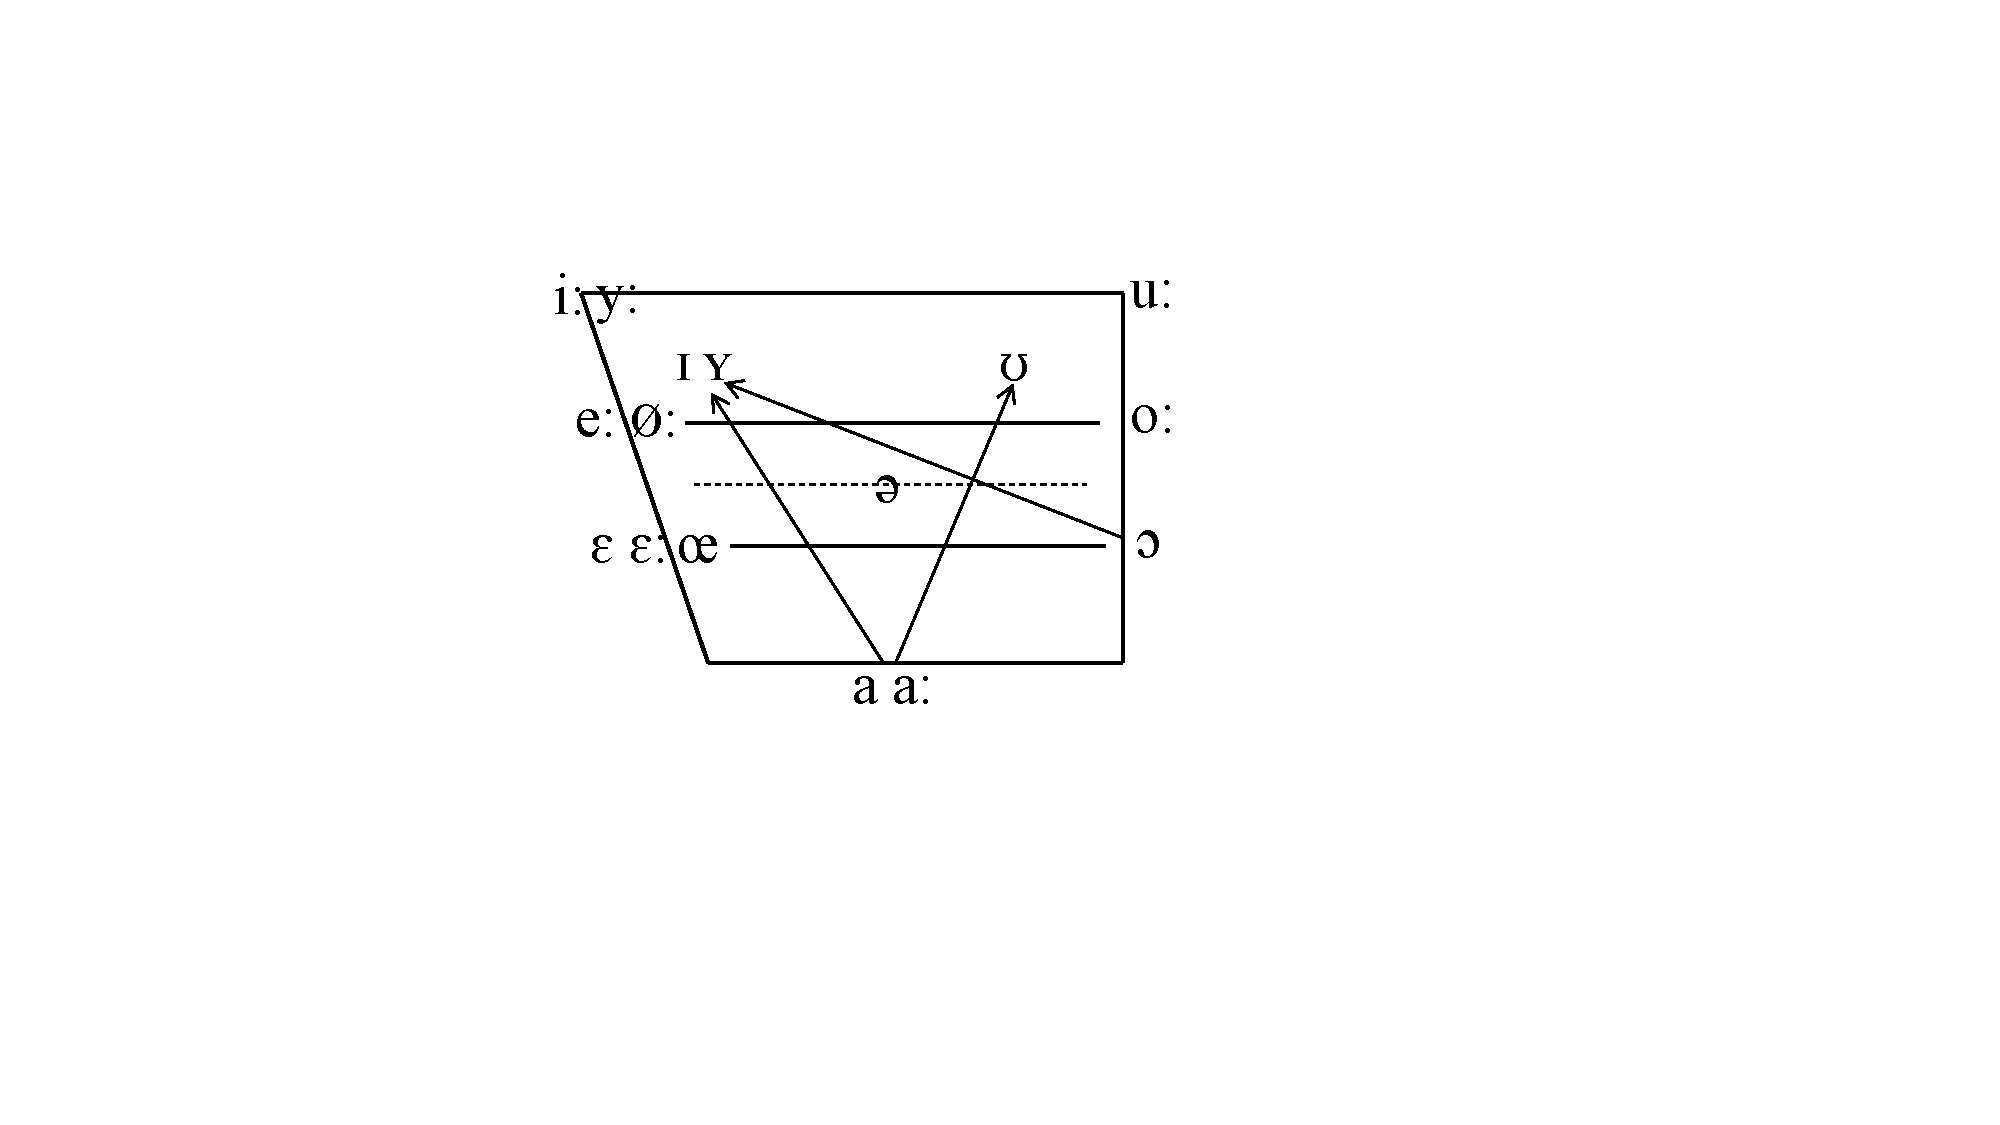
\includegraphics[width=.5\textwidth]{figures/Vokalviereck_Phoneme.pdf}
    \caption{Phonemische deutsche Vokale nach \citet{Hall2000}.\label{fig:Vokalviereck_phonemisch}}
\end{figure}


\begin{table}
\centering
\footnotesize
\caption{Phoneminventar des Deutschen angelehnt an \citet[62, 68]{Hall2000}\label{tab:Phoneminventar}}
\resizebox{\textwidth}{!}{
\begin{tabular}{llll}\lsptoprule
Phonem & Minimalpaar&Phonem & Minimalpaar\\\midrule
\textipa{/p/} & \textit{Pein} \textipa{[p\t*{aI}n]} -- \textit{Bein} \textipa{[b\t*{aI}n]} & \textipa{/a/}& \textit{Bann} \textipa{[ban]} -- \textit{Bahn} \textipa{[ba:n]} \\
\textipa{/b/} & \textit{Bein} \textipa{[b\t*{aI}n]} -- \textit{kein} \textipa{[k\t*{aI}n]} & \textipa{/a:/}& \textit{Rasen} \textipa{[Ka:.z@n]} -- \textit{Rosen} \textipa{[Ko:.z@n]} \\
\textipa{/t/} & \textit{Teich} \textipa{[t\t*{aI}\c{c}]} -- \textit{Deich} \textipa{[d\t*{aI}\c{c}]} & \textipa{/i:/}& \textit{Miete} \textipa{[\textprimstress mi:.t@]} -- \textit{Mitte} \textipa{[\textprimstress mI\.*{t}@]} \\
\textipa{/d/} & \textit{schade} \textipa{[\textprimstress Sa:.d@]} -- \textit{Schale} \textipa{[\textprimstress Sa:.l@]} & \textipa{/I/}& \textit{Mitte} \textipa{[\textprimstress mI\.*t@]} -- \textit{Motte} \textipa{[\textprimstress mO\.*t@]} \\
\textipa{/k/} & \textit{Ecke} \textipa{[\textprimstress PE\.*k@]} -- \textit{Egge} \textipa{[\textprimstress PE\.*g@]} & \textipa{/y:/}& \textit{wühlen} \textipa{[\textprimstress vy:.l@n]} -- \textit{Wahlen} \textipa{[\textprimstress va:.l@n]} \\
\textipa{/g/} & \textit{Geiz} \textipa{[g\t*{aI}\t{ts}]} -- \textit{Reiz} \textipa{[K\t*{aI}\t{ts}]} & \textipa{/Y/}& \textit{Hütte} \textipa{[\textprimstress hY\.*{t}@]} -- \textit{Hüte} \textipa{[\textprimstress hy:.t@]} \\
\textipa{/\t{pf}/} & \textit{Topf} \textipa{[tO\t{pf}]} -- \textit{toll} \textipa{[tOl]} & \textipa{/u:/} & \textit{gut} \textipa{[gu:t]} -- \textit{Gott} \textipa{[gOt]}\\
\textipa{/\t{ts}/} & \textit{Zopf} \textipa{[\t{ts}O\t{pf}]} -- \textit{Topf} \textipa{[tO\t{pf}]} & \textipa{/U/} &\textit{Butter} \textipa{[\textprimstress bU\.*{t}5]} -- \textit{bitter} \textipa{[\textprimstress bI\.*{t}5]}\\
\textipa{/\t{tS}/} & \textit{Kutsche} \textipa{[\textprimstress kU\.*{\t{tS}}@]} -- \textit{Kuppe} \textipa{[\textprimstress kU\.*{p}@]}& \textipa{/e:/} & \textit{beten} \textipa{[\textprimstress be:.t@n]} -- \textit{Betten} \textipa{[\textprimstress bE\.*{t}@n]}\\
\textipa{/\t{dZ}/}& \textit{Gin} \textipa{[\t{dZ}In]} -- \textit{Kinn} \textipa{[kIn]} & \textipa{/E/} & \textit{Welt} \textipa{[vElt]} -- \textit{Wald} \textipa{[valt]}\\
\textipa{/f/} & \textit{fein} \textipa{[f\t*{aI}n]} -- \textit{Wein} \textipa{[v\t*{aI}n]} &\textipa{/E:/} & \textit{säen} \textipa{[\textprimstress zE:.@n]} -- \textit{sehen} \textipa{[\textprimstress ze:.@n]}\\
\textipa{/v/} & \textit{Wein} \textipa{[v\t*{aI}n]} -- \textit{kein} \textipa{[k\t*{aI}n]} &\textipa{/o:/} & \textit{Ofen} \textipa{[\textprimstress Po:.f@n]} -- \textit{offen} \textipa{[\textprimstress PO\.*{f}@n]}\\
\textipa{/s/} & \textit{Masse} \textipa{[\textprimstress ma\.*s@]} -- \textit{Masche} \textipa{[\textprimstress ma\.*S@]} & \textipa{/O/} & \textit{locker} \textipa{[\textprimstress lO\.*k5]} -- \textit{lecker} \textipa{[\textprimstress lE\.*k5]}\\
\textipa{/z/} & \textit{Besen} \textipa{[\textprimstress be:.z@n]} -- \textit{beten} \textipa{[\textprimstress be:.t@n]} & \textipa{/\o:/}& \textit{Böden} \textipa{[\textprimstress b\o:.d@n]} -- \textit{Boden} \textipa{[\textprimstress bo:.d@n]}\\
\textipa{/S/} & \textit{Schuh} \textipa{[Su:]} -- \textit{Kuh} \textipa{[ku:]} & \textipa{/\oe/}& \textit{löschen} \textipa{[\textprimstress l\oe \.*S@n]} -- \textit{Laschen} \textipa{[\textprimstress la\.*S@n]}\\
\textipa{/Z/} & \textit{Jacques} \textipa{[Zak]} -- \textit{Pack} \textipa{[pak]} &\textipa{/@/} & \textit{Motte} \textipa{[\textprimstress mO\.*{t}@]} -- \textit{Motto} \textipa{[\textprimstress mO\.*{t}o]}\\
\textipa{/\c{c}/} & \textit{mich} \textipa{[mI\c{c}]} -- \textit{mit} \textipa{[mIt]} &\textipa{/\t*{aI}/}& \textit{leise} \textipa{[\textprimstress l\t*{aI}.z@]} -- \textit{Läuse} \textipa{[\textprimstress l\t*{OI}.z@]}\\
\textipa{/h/} & \textit{Haus} \textipa{[h\t*{aU}s]} -- \textit{Maus} \textipa{[m\t*{aU}s]} & \textipa{/\t*{aU}/}& \textit{Laus} \textipa{[l\t*{aU}s]} -- \textit{lies} \textipa{[li:s]}\\
\textipa{/m/} & \textit{mein} \textipa{[m\t*{aI}n]} -- \textit{nein} \textipa{[n\t*{aI}n]} & \textipa{/\t*{OI}/}& \textit{Leute} \textipa{[\textprimstress l\t*{OI}.t@]} -- \textit{Laute} \textipa{[\textprimstress l\t*{aU}.t@]}\\
\textipa{/n/} & \textit{nah} \textipa{[na:]} -- \textit{da} \textipa{[da:]}&&\\
\textipa{/N/} & \textit{Enge} \textipa{[\textprimstress PE\.*N@]} -- \textit{Ecke} \textipa{[\textprimstress PE\.*k@]}&&\\
\textipa{/l/} & \textit{lang} \textipa{[laN]} -- \textit{Gang} \textipa{[gaN]}&&\\
\textipa{/K/} & \textit{Reiter} \textipa{[\textprimstress K\t*{aI}.t5]} -- \textit{Leiter} \textipa{[\textprimstress l\t*{aI}.t5]}&&\\
\textipa{/j/}& \textit{Jahr} \textipa{[ja:]} -- \textit{wahr} \textipa{[va:]}&&\\
\lspbottomrule
\end{tabular}}
\end{table}
\normalsize

\clearpage



\section{Die Silbe} \label{subsec:Silbe}

Silben\is{Silbe} sind, wie \citet{Keating1983} durch die Untersuchung von Kieferbewegungen gezeigt hat, motorisch gesehen Öffnungs- und Schließbewegungen des Vokal\-trakts. Um das nachzuvollziehen, kann man ein Wort wie \textit{Mama} sprechen und dabei den Zeigefinger an das Kinn legen. Man wird feststellen, dass der Kiefer für jede Silbe einmal abgesenkt wird. Wenn der Vokal einer Silbe nicht \textipa{/a/} ist, ist die Kieferbewegung kleiner oder aber es bewegt sich nur die Zunge vom Gaumen weg (etwa bei \textit{Susi}). Auf jeden Fall gibt es pro Silbe eine Öffnungsbewegung und zur nächsten Silbe hin eine Schließbewegung. Aus dieser artikulatorischen Eigenschaft von Silben ergibt sich eine sehr prominente akustische Eigenschaft von Silben, die Sonorität. Um die Sonorität geht es in Abschnitt~\ref{subsec:Sonoritaet}. Den Beginn des Abschnitts zur Silbe bildet aber Abschnitt \ref{subsec:Betonbarkeit}, in welchem es um den Unterschied zwischen betonbaren und nicht betonbaren Silben geht. Das Thema von Abschnitt~\ref{subsec:Silbifizierung} ist die Silbifizierung, das heißt die Zuordnung von Lauten zu Silben innerhalb von Wörtern. In Abschnitt~\ref{subsec:Silbenkonstituenten} wird das Konstituentenstrukturmodell der Silbe vorgestellt. 



\subsection{Betonbare und nicht betonbare Silben}\label{subsec:Betonbarkeit}

Man unterscheidet zwischen betonbaren und nicht betonbaren Silben. Nicht betonbare Silben können unter keinen Umständen betont werden. Eine nicht betonbare Silbe ist etwa \textipa{[g@]} in \textit{Liege} \textipa{[\textprimstress li:.g@]} oder \textipa{[t5]} in \textit{Meister} \textipa{[\textprimstress m\t*{aI}s.t5]}. Betonbare Silben können betont werden, müssen es aber nicht. \textipa{[lUN]} etwa ist in \textit{Lunge} \textipa{[\textprimstress lU\.*N@]} betont, in \textit{Sammlung} \textipa{[\textprimstress zam.lUN]} jedoch nicht. \textipa{[nIs]} ist in \textit{nisten} \textipa{[\textprimstress nIs.t@n]} betont, in \textit{Kenntnis} \textipa{[\textprimstress kEnt.nIs]} jedoch nicht.

Betonbare Silben beginnen immer mit einem Konsonanten. Wenn -- orthografisch -- kein Konsonant vor dem Vokal steht, wird der Knacklaut produziert. Die zweite Silbe in \textit{feiern} \textipa{[\textprimstress f\t*{aI}.5n]} oder \textit{freuen} \textipa{[\textprimstress fK\t*{OI}.@n]} ist nicht betonbar, weil diese Silben nicht mit Konsonant beginnen.

Betonbare Silben weisen darüber hinaus über eins der drei folgenden Segmente bzw. Segmentkombinationen auf:
\begin{itemize}
\item ein gespannter Vokal, \zB in der ersten Silbe von \textit{sagen} \textipa{[\textprimstress za:.g@n]} bzw. \textipa{[\textprimstress za:.g\s{N}]}
\item ein Diphthong, \zB in der ersten Silbe von \textit{sauber} \textipa{[\textprimstress z\t*{aU}.b5]} oder der zweiten von \textit{genau} \textipa{[g@\textprimstress n\t*{aU}]}
\item ein ungespannter Vokal plus ein oder mehrere dem Vokal folgende Konsonanten. \zB in \textit{Sinn} \textipa{[\textprimstress zIn]} oder \textit{Sand} \textipa{[\textprimstress zant]}.
\end{itemize}

Silben, deren Nukleus mit Schwa besetzt ist, sind grundsätzlich nicht betonbar, selbst wenn sonst alle Bedingungen für Betonbarkeit gegeben sind, \zB die zweite Silbe von \textit{Segel }\textipa{[\textprimstress ze:.g@l]}.


\subsection{Die Sonoritätshierarchie}\label{subsec:Sonoritaet}
\is{Sonorität}
\is{Sonoritätshierarchie}
Das Zerlegen von Wörtern in Silben oder das Benennen der Silbenanzahl eines Wortes ist eine Kompetenz, die häufig schon in der Vorschule erworben wird. Viele Schulanfänger können beispielsweise angeben, dass ein Wort wie \textit{Schule} oder \textit{Kinder} zwei Silben hat. Wörter in Silben zu zerlegen ist damit eine Kompetenz, die früher erworben wird als die Extraktion von Anlauten oder gar die Durchgliederung von Wörtern in Laute \citep{ZieglerGoswami2005}. Das liegt daran, dass Silben eine auditiv sehr prominente Eigenschaft haben: ihren Sonoritätsverlauf. 

Unter \textit{Sonorität} versteht man die Schallfülle oder Lautstärke eines Lautes \citep[59--60]{NoackPhonologie2016}. Die Sonorität ist abhängig vom Öffnungsgrad des Vokaltrakts. Laute wie \textipa{[a, E]}, die mit offenem Mund produziert werden, haben eine höhere Sonorität (sie sind lauter) als Laute wie \textipa{[t, k]}, die durch einen oralen Verschluss charakterisiert sind.

Die Abfolge der Laute in einer Silbe ist zu einem großen Teil durch die Sonorität bestimmt (\zB \cite[224]{Hall2000}). Laute, bei denen der Mund offen ist -- das sind vor allem die Vokale -- stehen in der Mitte einer Silbe. Geschlossenere Laute stehen am Rand einer Silbe. Das ist in Abbildung~\ref{Abb:Sonoritaet} dargestellt. In dieser Abbildung symbolisiert die ansteigende und abfallende Linie den Sonoritätsverlauf über eine Silbe. Die Klassifikation der Laute in \is{Obstruent}\is{Nasal}\is{Liquid}\is{Vokal}Obstruenten,\footnote{Obstruenten sind Plosive, Frikative und Affrikaten (vgl. Abschnitt~\ref{sec:ObstSon}).} Nasale, Liquide und Vokale wird im Folgenden mit Hilfe der in der Abbildung angegebenen Beispiele erklärt.



\begin{figure}
    \centering
    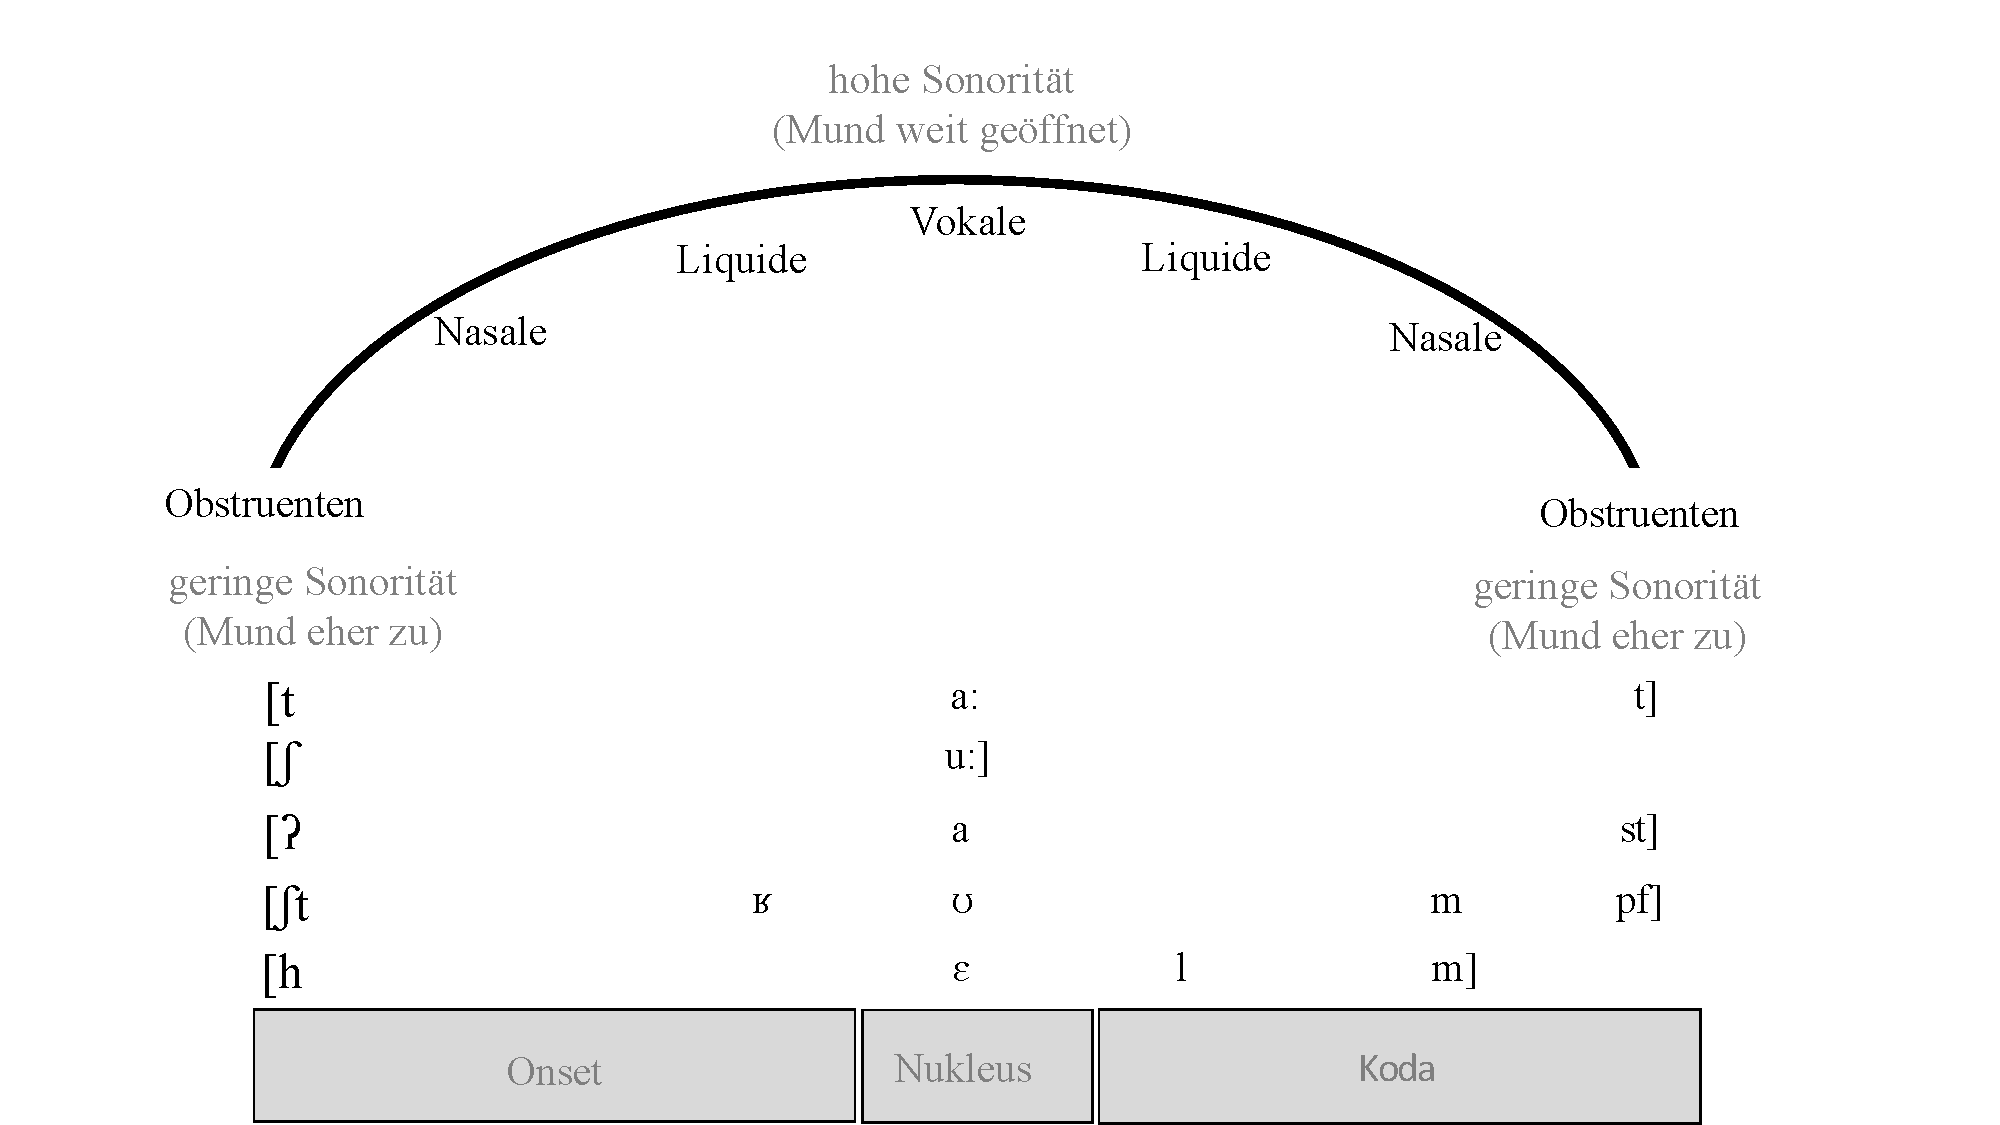
\includegraphics[width=1\textwidth]{figures/Sonoritaet.pdf}
    \caption{Sonoritätsverlauf in der Silbe nach \citet[224]{Hall2000}}
    \label{Abb:Sonoritaet}
\end{figure}




Das erste Beispiel, die Silbe \textit{Tat} \textipa{[ta:t]}, beginnt mit einem sehr wenig sonoren Laut, dem Obstruenten \textipa{[t]}, dem ein sehr sonorer Laut folgt, der Vokal \textipa{[a:]}. Am Ende steht wieder ein sehr wenig sonorer Laut, der Obstruent \textipa{[t]}. Wenn man die Laute vertauscht und eine Sequenz wie \textipa{[ata]} bildet, dann besteht diese Sequenz aus zwei Silben, denn die Sonorität fällt zunächst und steigt dann wieder an.

Das \is{Silbe!offen}zweite Beispiel in Abbildung~\ref{Abb:Sonoritaet}, \textit{Schuh} \textipa{[Su:]}, zeigt, dass Silben auch mit Vokal enden können. Die Schließbewegung des Mundes und der dadurch produzierte Abfall der Sonorität ist also optional. Solche Silben nennt man \textit{offene Silben}. Silben, bei denen dem Vokal noch ein Konsonant folgt, nennt man \is{Silbe!geschlossen}\textit{geschlossene Silben}.

Am dritten Beispiel, \textit{Ast} \textipa{[Past]}, kann man erkennen, dass betonte Silben im Deutschen jedoch nicht hochsonor beginnen können, also nicht mit einem Vokal. Vor dem Vokal muss mindestens ein Konsonant stehen. Sollte dies nicht der Fall sein, wird der Knacklaut als eine Art Dummy-Konsonant eingesetzt (vgl. Abschnitt~\ref{sec:Epenthese}). So entspricht auch eine Silbe wie \textit{Ast} \textipa{[Past]}  der Sonoritätshierarchie.

Das\is{Sonorant}\is{Obstruent} vierte Beispiel, \textit{Strumpf}, zeigt, dass nicht alle Konsonanten gleich sonor sind und die Konsonanten deshalb nicht in jeder beliebigen Reihenfolge auftreten können.\is{Nasal}\is{Lateral}\is{Vibrant}\is{Approximant} \textipa{[K]} und \textipa{[m]} sind als \is{Sonorant}Sonoranten\footnote{Sonoranten sind Nasale, Laterale, Vibranten und Approximanten (vgl. Abschnitt~\ref{sec:ObstSon}).}\footnote{Auch wenn \textipa{[K]} phonetisch gesehen ein Frikativ ist, zählt er innerhalb der Sonoritätsanalysen als Sonorant. Das liegt daran, dass das frikativische Allophon \textipa{[K]} nur eine Möglichkeit ist, den Konsonanten zu produzieren. Die vibrantischen Allophone \textipa{[r, \;R]} sind älter und hatten dadurch mehr Einfluss auf die Silbenstruktur der Wörter des Deutschen.} sonorer als die Obstruenten \textipa{[S, t, \t{pf}]}. Eine Sequenz wie \textipa{[KStU\t{pf}m]} ist keine mögliche Silbe, weil die sonoren Konsonanten \textipa{[K]} und \textipa{[m]} nicht weiter außen stehen können als die weniger sonoren Laute \textipa{[S, t, \t{pf}]}.

Innerhalb der Klasse der Sonoranten gibt es jedoch auch noch wesentliche Unterschiede in der Sonorität. So ist eine Silbe wie \textit{Helm} \textipa{[hElm]} (letztes Beispiel in Abbildung~\ref{Abb:Sonoritaet}) möglich, eine Sequenz wie \textipa{[hEml]} ist jedoch zweisilbig. Deshalb unterscheidet man innerhalb der Sonoranten noch zwischen den sogenannten \textit{Liquiden}\is{Liquid} (im Deutschen \textipa{/l/, /j/} und alle \textipa{/K/}-Allophone) und den Nasalen \textipa{/m, n, N/}. Die Liquide sind offener und stehen deshalb direkt um den Vokal herum. Die Nasale sind geschlossener und stehen zwischen den Obstruenten und den Liquiden.\footnote{Nasale werden, wie Plosive, mit einem totalen oralen Verschluss gebildet. Sie sind trotzdem sonorer als die Plosive, weil die Nasalpassage zum Vokaltrakt zählt, und diese Passage bei den Nasalen (im Unterschied zu den Plosiven) offen ist (vgl. Abschnitt~\ref{subsec:Nasale}).}

Eine \is{Onset}\is{Nukleus}\is{Koda}betonbare Silbe besteht also aus einem vokalischen Kern, um den sich Liquide, Nasale und Obstruenten wie die Häute einer Zwiebel positionieren.\footnote{Diese sehr einfache Klassifikation der Laute nach ihrer Sonorität ist für unsere Zwecke ausreichend. Eine feingliedrigere Einteilung findet man beispielsweise bei \citet[132]{RamersVater1991}, die Plosive als weniger sonor einstufen als Frikative, \textipa{[l]} als weniger sonor betrachten als \textipa{[K]} und zwischen hohen und tiefen Vokalen unterscheiden. \citet[72]{Wiese2011} folgt dem. \citet[61]{NoackPhonologie2016} übernimmt die Klassifikation von \citet{Jespersen1904}, der zusätzlich eine höhere So\-norität für stimmhafte Plosive und Frikative annimmt als für stimmlose. \textipa{[l]} und \textipa{[K]} werden als gleich sonor analysiert.} Den vokalischen Kern bezeichnet man, wie wir schon in Abschnitt~\ref{sec:KonsonantenundVokale} gesehen haben, als \textit{Nukleus}. Die Konsonanten die in der Silbe vor dem Nukleus stehen, nennt man den \textit{Onset} der Silbe. Alle Konsonanten, die dem Nukleus in der Silbe folgen, bilden die \textit{Koda} der Silbe. Silben können im Deutschen einen oder mehrere Konsonanten im Onset haben. Die Koda kann leer sein, sie kann aber auch mit einem oder mehreren Konsonanten besetzt sein. Die Konsonanten im Onset müssen so angeordnet sein, dass die Sonorität zum Nukleus hin ansteigt. Die Konsonanten in der Koda müssen so angeordnet sein, dass die Sonorität vom Nukleus her abfällt.

Mittels dieses Modells kann man nicht nur die Struktur von existierenden und möglichen Silben des Deutschen erklären, sondern auch die Lage von Silbengrenzen. Ein Wort wie \textit{Hamster} kann nicht als \textit{Ha-mster} silbifiziert werden, denn das \textipa{[m]} hat als Sonorant eine höhere Sonorität als der Frikativ \textipa{[s]} und kann deshalb nicht weiter vom Vokal der Silbe entfernt stehen als das \textipa{[s]}.


\subsection{Silbifizierung}\is{Silbifizierung}\label{subsec:Silbifizierung}

Für die Silbifizierung, also die Zuordnung von Lauten eines Wortes zu einzelnen Silben, gibt es unterschiedliche Gesetzmäßigkeiten. Diese Gesetzmäßigkeiten gehören zum impliziten Wissen von Sprecherinnen und Sprechern einer Sprache und erlauben es ihnen, weitgehend intuitiv zu silbifizieren. Der wichtigste Hinweis auf eine Silbengrenze kommt wie schon angedeutet über die Sonorität\is{Sonorität}: Silbengrenzen liegen im Deutschen in der Regel vor einem (lokalen) Sonoritätsminimum. 

Als Beispiel für diese Art der Lokalisierung der Silbengrenze sollen die Wörter \textit{Palme} und \textit{dreisilbig} betrachtet werden. Sprecherinnen und Sprecher des Deutschen silbifizieren diese Wörter \textit{Pal-me} und \textit{drei-sil-big}. In Abbildung~\ref{Abb:Silbifizierung} ist der Sonoritätsverlauf, den die Sprecherinnen und Sprecher akustisch wahrnehmen, als Kurve dargestellt. Die horizontale Achse zeigt die Abfolge der Laute, die vertikale Achse die Sonorität der einzelnen Laute.

Die erste Silbe von \textit{Palme} (oberer Teil der Abbildung), \textipa{[pal]}, besteht aus dem Obstruenten \textipa{[p]}, dem Vokal \textipa{[a]} und dem Sonoranten \textipa{[l]}. Die Sonorität steigt also von \textipa{[p]} zu \textipa{[a]} an und sinkt dann wieder für \textipa{[l]}. \textipa{[m]} hat eine geringere Sonorität als \textipa{[l]}. Da die Sonorität für das Schwa wieder ansteigt, ist \textipa{[m]} also das Sonoriätsminimum\is{Sonoritätsminimum} zwischen den beiden Vokalen. Die Silbengrenze\is{Silbengrenze} wird vor dieses Minimum gesetzt (gestrichelte Linie), deshalb silbifiziert man \textit{Pal-me} und nicht etwa \textit{Pa-lme} oder \textit{Palm-e}.\footnote{Die Silbifizierung \textit{Pal-me} schließt nicht aus, dass es Silben wie \textit{palm} geben könnte. Wenn ein Wort durch Derivation oder Flexion zweisilbig wird, kommt es häufig zu einer Verschiebung der Silbengrenze, um den Anforderungen bezüglich der Sonorität gerecht zu werden: \textit{Helm -- Hel-me, Wind -- win-dig}.}



\begin{figure}
    \centering
\begin{center}
	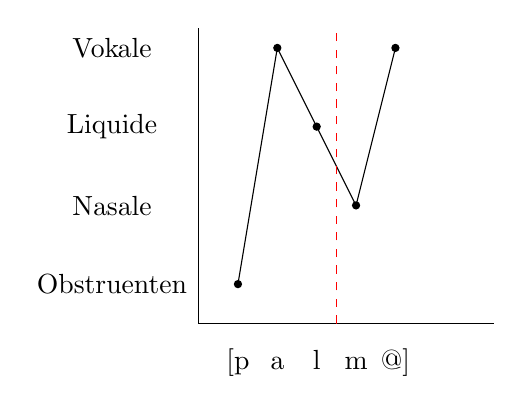
\begin{tikzpicture}[scale=0.5]
		\draw[black] (-1,0) -- (6.5,0) ; % x axis
		\draw[black] (-1,0) -- (-1,7.5); % y axis
		\node at (-3.2,1) {Obstruenten};
		\node at (-3.2,3) {Nasale};
		\node at (-3.2,5) {Liquide};
		\node at (-3.2,7) {Vokale};
		\draw[black] (0,1) -- (1,7) -- (2,5) -- (3,3) -- (4,7);
		\node at (0,-1) {\strut \textipa{[p}};
		\node at (1,-1) {\strut \textipa{a}};
		\node at (2,-1) {\strut \textipa{l}};
		\node at (3,-1) {\strut \textipa{m}};
		\node at (4,-1) {\strut \textipa{@}]};
		\fill (0,1) circle [radius=3pt];
		\fill (1,7) circle [radius=3pt];
		\fill (2,5) circle [radius=3pt];
		\fill (3,3) circle [radius=3pt];
		\fill (4,7) circle [radius=3pt];
        \draw[red, dashed] (2.5,0) -- (2.5,7.5);
	\end{tikzpicture}

    	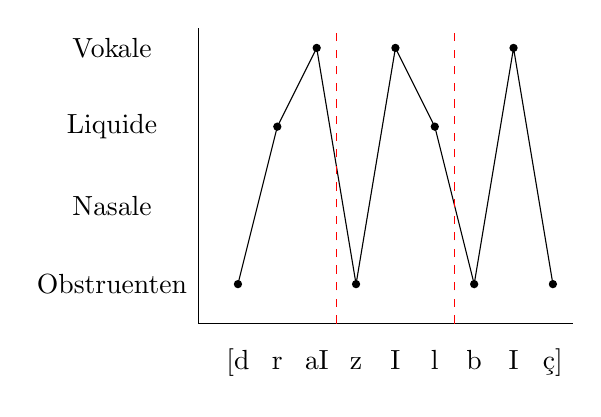
\begin{tikzpicture}[scale=0.5]
		\draw[black] (-1,0) -- (8.5,0) ; % x axis
		\draw[black] (-1,0) -- (-1,7.5); % y axis
		\node at (-3.2,1) {Obstruenten};
		\node at (-3.2,3) {Nasale};
		\node at (-3.2,5) {Liquide};
		\node at (-3.2,7) {Vokale};
		\draw[black] (0,1) -- (1,5) -- (2,7) -- (3,1) -- (4,7) -- (5,5) -- (6,1) -- (7,7) -- (8,1);
		\node at (0,-1) {\strut \textipa{[d}};
		\node at (1,-1) {\strut \textipa{r}};
		\node at (2,-1) {\strut \textipa{aI}};
		\node at (3,-1) {\strut \textipa{z}};
		\node at (4,-1) {\strut \textipa{I}};
		\node at (5,-1) {\strut \textipa{l}};
		\node at (6,-1) {\strut \textipa{b}};
        \node at (7,-1) {\strut \textipa{I}};
        \node at (8,-1) {\strut \textipa{\c{c}]}};
		\fill (0,1) circle [radius=3pt];
		\fill (1,5) circle [radius=3pt];
		\fill (2,7) circle [radius=3pt];
		\fill (3,1) circle [radius=3pt];
		\fill (4,7) circle [radius=3pt];
		\fill (5,5) circle [radius=3pt];
		\fill (6,1) circle [radius=3pt];
        \fill (7,7) circle [radius=3pt];
        \fill (8,1) circle [radius=3pt];
        \draw[red, dashed] (2.5,0) -- (2.5,7.5);% -- (5,6) -- (6,3);
        \draw[red, dashed] (5.5,0) -- (5.5,7.5);% -- (5,6) -- (6,3);
	\end{tikzpicture}
	
\end{center}
    
    \caption{Silbifizierung. Auf der vertikalen Achse ist die Sonorität der einzelnen Laute dargestellt. Die horizontale Achse zeigt die zeitliche Abfolge der Laute. Die gestrichelte Linien zeigt die Silbengrenze an.}
    \label{Abb:Silbifizierung}
\end{figure}

Bei dem Wort \textit{dreisilbig} (unterer Teil der Abbildung) beginnt die erste Silbe mit dem Obstruenten\is{Obstruent} \textipa{[d]}. Danach steigt die Sonorität an, zunächst zum zweiten Laut, dem Liquid \textipa{[K]}, und dann zum dritten, dem Vokal \textipa{[\t*{aI}]}. Danach fällt sie zum \textipa{[z]} hin ab, bevor sie zum \textipa{[I]} hin wieder ansteigt. Das \textipa{[z]} bildet also ein Minimum, sodass davor die erste Silbengrenze liegt. Vom \textipa{[I]} fällt die Sonorität über \textipa{[l]} zum \textipa{[b]} ab, bevor sie zum zweiten \textipa{[I]} wieder ansteigt. Das \textipa{[b]} bildet also wieder ein Sonoritätsminimum\is{Sonoritätsminimum}, sodass die zweite Silbengrenze\is{Silbengrenze} vor dem \textipa{[b]} liegt. 

Mittels der Sonorität\is{Sonorität} lassen sich viele, aber längst nicht alle Silbengrenzen begründen. Vor allem bei Konsonantenclustern\is{Konsonantencluster} ist die Sonorität als Erklärung für die Lage der Silbengrenzen nicht ausreichend. Als Beispiel dazu wird hier das Wort \textit{extrem} \textipa{[PEks\textprimstress tKe:m]} betrachtet. Laut Sonorität sollte man \textit{e-xtrem} \textipa{[PE\textprimstress kstKe:m]} silbifizieren,\is{Sonorität}\is{Silbifizierung} denn das Sonoritätsminimum ist bei \textipa{[k]} erreicht. Man silbifiziert jedoch \textit{ex-trem} \textipa{[PEks\textprimstress tKe:m]}.

Für\is{Phonotaktik}\is{Phonotaktik} die Abfolge von Lauten im Onset und in der Koda gibt es in jeder Sprache sogenannte \textit{phonotaktische Regeln} (vgl. Abschnitt~\ref{subsec:Phonotaktik}), die bestimmen, welche Laute in welcher Position und in welcher Kombination vorkommen können. Die phonotaktischen Regeln für das Deutsche schließen Sequenzen wie \textipa{[kstK]} im Onset einer Silbe aus, denn im Deutschen können maximal drei Konsonanten im Onset stehen \citep[68--69]{Hall1992}. Eine Silbe kann also nicht mit \textipa{[kstK]} beginnen. Auch \textipa{[stK]} ist vor dem Vokal im Standard nicht möglich. Zwar sind \textipa{/S/} und \textipa{/s/} (und nur diese beiden) als erste von drei Konsonanten im Onset möglich, das \textipa{/s/} verbindet sich dabei aber nur mit \textipa{/kK/} oder \textipa{/kl/} und selbst das nur in einigen Lehnwörtern (\textit{Skrupel, Sklave}). Die Silbengrenze bei \textit{extrem} wird also an der frühestmöglichen Position gesetzt, und die liegt nach dem \textipa{/s/}: \textipa{[PEks\textprimstress tKE:m]}.

Unabhängig davon sind Silbengrenzen durch den morphologischen Aufbau der Wörter beeinflusst \citep[72--73]{Bergmann2018}. Das Wort \textit{enteisen} beispielsweise wird \textit{ent-ei-sen} silbifiziert, obwohl die erste Silbengrenze laut Sonorität vor dem \textipa{/t/} stehen müsste (\textit{en-tei-sen}). Bei \textit{ent-} handelt es sich jedoch um ein \is{Präfix}Präfix. Präfixe verändern die Silbenstruktur der nachfolgenden Morpheme in der Regel nicht. Die Silbengrenze ist deshalb identisch mit der Morphemgrenze.

Eine Suffigierung\is{Suffigierung}\is{Suffix} hingegen kann zu einer Resilbifizierung führen \citep[73--74]{Bergmann2018}. Suffixe mit vokalischem Onset lösen eine Verschiebung der Silbengrenze nach links aus. So silbifiziert man \textit{Lö-sung} und nicht (nach Morphemen) \textit{Lös-ung}.

\subsection{Das Konstituentenstrukturmodell}\label{subsec:Silbenkonstituenten}\is{Konstituentenstrukturmodell}

In der Schriftsprachvermittlung wird inzwischen vielfach das sogenannte \textit{Häusermodell} (vgl. Exkurs~\ref{ex:SAM_Grundlage}, Seite~\pageref{ex:SAM_Grundlage}) genutzt, um Lernende mit der Struktur der Silbe vertraut zu machen und silbenspezifische Aussprache- und Orthografieregeln abzuleiten. In diesem Abschnitt geht es um das linguistische Modell, welches die Grundlage für das Häusermodell bildet.

\subsubsection{Onset, Nukleus und  Koda}

\is{Onset}\is{Nukleus}\is{Koda}Bei der Betrachtung der Sonorität wurde festgestellt, dass eine Silbe in der Regel aus einem vokalischen Kern besteht, der von Konsonanten umgeben ist. Den vokalischen Kern bezeichnet man als \textit{Nukleus}. Die Konsonanten vor dem Nukleus bilden den \textit{Onset}. Optional können dem Vokal noch Konsonanten folgen. Diese Konsonanten bilden die \textit{Koda} der Silbe. Man könnte eine Silbe also so darstellen wie in Abbildung~\ref{Abb:Silbenstruktur1}. Das σ (gesprochen \textit{Sigma}, griechisch für den Laut \textipa{[s]}) steht dabei für die Silbe, welche sich in Onset, Nukleus und Koda unterteilt. Eine solche Struktur nimmt für das Deutsche beispielsweise \citet[42--43]{Hall1992} an.

\begin{figure}
  \centering
  \begin{forest}
      [σ
        [Onset, ake
                  ]
          [Nukleus, ake
                    ]
          [Koda, ake
                    ]
      ]
  \end{forest}
  \caption{Eine mögliche Silbenstrukturanalyse nach \citet{Hall1992}}
    \label{Abb:Silbenstruktur1}
\end{figure}
\is{Onset}\is{Nukleus}\is{Koda}


\begin{Definition}{Onset, Nukleus und Koda}\label{def:OnsetNukleusKoda}

\noindent
Eine Silbe besteht aus Onset, Nukleus und Koda. Der Onset\is{Onset} einer Silbe besteht aus den Konsonanten, die vor dem Vokal stehen. Im Nukleus einer betonbaren Silbe steht ein vokalisches Segment. Die Koda besteht aus Konsonanten, die dem Vokal folgen.
\end{Definition}



\subsubsection{Reim}\label{subsec:Reim}\is{Reim}
\citet[134]{RamersVater1991} nehmen an, dass Nukleus und Koda enger miteinander verbunden sind als der Onset mit dem Nukleus. Wir folgen dem und werden deshalb ein etwas komplexeres Modell annehmen als das in Abbildung~\ref{Abb:Silbenstruktur1}, nämlich das Modell  in Abbildung~\ref{Abb:Silbenstruktur2} Bei diesem Modell werden Nukleus und Koda zunächst zu einem \textit{Reim} zusammengefasst. Erst in einem zweiten Schritt entsteht die Silbe aus Onset und Reim.
\is{Silbenstrukturanalyse}


\begin{figure}
  \centering
  \begin{forest}
      [σ, calign=last
        [Onset, ake
                  ]
        [Reim, calign=first
          [Nukleus, ake
                    ]
          [Koda, ake
                    ]
        ]
      ]
  \end{forest}
  \caption{Silbenstrukturanalyse mit Reim nach \citet{RamersVater1991}}
    \label{Abb:Silbenstruktur2}
\end{figure}

Für die Annahme des Reims gibt es unterschiedliche Argumente und Gegenargumente. Wir diskutieren hier drei davon, nämlich den Längenausgleich zwischen Nukleus und Koda, den poetischen Effekt von Reimen und Evidenz aus der Versprecherforschung. \citet[134--135]{RamersVater1991}\is{Längenausgleich} diskutieren den \textit{Längenausgleich} zwischen Nukleus und Koda, den man so formulieren kann: Wenn in einer Silbe viel Material im Nukleus ist, ist tendenziell wenig Material in der Koda. Wenn wenig Material im Nukleus ist, ist tendenziell mehr Material in der Koda. Tabelle~\ref{tab:Laengenausgleich} gibt einige Beispiele.

\begin{table}
\centering
\caption{Längenausgleich zwischen Nukleus und Koda. Die Zeilen entsprechen unterschiedlich komplexen Onsets (C=Konsonant), die Spalten unterschiedlich komplexen Kodas. Das jeweils erste Wort in jeder Zelle enthält einen Langvokal (LV), das zweite einen Kurzvokal (KV). \label{tab:Laengenausgleich}}
\begin{tabular}{lllllll}\lsptoprule
                &    \multicolumn{2}{c}{Koda leer}         &  \multicolumn{2}{c}{Koda C}         & \multicolumn{2}{c}{Koda CC} \\\midrule
      Onset          & LV & KV & LV & KV & LV & KV\\\midrule
C               & \textit{roh}& \textit{--}    & \textit{Moos} & \textit{Biss}     &  \textit{Mond} & \textit{Wunsch}\\ 
               & \textipa{[Ko:]} &     &  \textipa{[mo:s]} &  \textipa{[bIs]}      &  \textipa{[mo:nt]}&  \textipa{[vUnS]}\\
CC              & \textit{Floh} & \textit{--}  & \textit{Floß}& \textit{flott}  &  \textit{--} & \textit{blond} \\ 
              & \textipa{[flo:]}&  & \textipa{[flo:s]}& \textipa{[flOt]}     &   &  \textipa{[blOnt]}\\ 
CCC             & \textit{Stroh} & \textit{--} & \textit{Strom} & \textit{Stress}    &  \textit{--} & \textit{Strand} \\ 
             & \textipa{[StKo:]}&  & \textipa{[StKo:m]}& \textipa{[StKEs]}   &   & \textipa{[StKant]}\\ 
\lspbottomrule
\end{tabular}
\end{table}

Die Zeilen der Tabellen repräsentieren unterschiedlich komplexe Onsets. In der ersten Zeile stehen Wörter mit einem Onset, der aus einem Konsonanten (C) besteht: \textit{roh, Moos, Biss} usw. In der zweiten Zeile stehen Wörter mit zwei Konsonanten im Onset: \textit{Floh, Floß} usw. In der dritten Zeile stehen Wörter mit drei Konsonanten im Onset: \textit{Stroh, Strom} usw.

Die Spalten zeigen Unterschiede in der Komplexität der Koda: In der ersten Spalte stehen Wörter mit leerer Koda, \textit{roh} \textipa{[Ko:]}, \textit{Floh} \textipa{[flo:]} usw., in der zweiten Wörter mit nur einem Konsonanten in der Koda, \textit{Moos} \textipa{[mo:s]}, \textit{Floß} \textipa{[flo:s]} usw., in der dritten Wörter mit zwei Konsonanten in der Koda, \textit{Mond} \textipa{[mo:nt]}, \textit{Wunsch} \textipa{[wUnS]}. Wörter mit drei oder mehr Konsonanten in der Koda sind in der Regel flektierte Wörter (\textit{springst, brauchst} usw.). Diese Wörter ignorieren wir und betrachten nur Simplizia.\footnote{morphologisch einfache Wörter} Es gibt nur wenige Simplizia mit drei oder vier Konsonanten in der Koda, etwa \textit{Text} \textipa{[tEkst]}, \textit{Axt} \textipa{[Pakst]} oder \textit{selbst} \textipa{[zElpst]}.

Das erste Wort in jeder Zelle, markiert mit LV, enthält einen Langvokal (also viel Material im Nukleus), \zB \textit{roh, Floß}. In zwei Zellen fehlt dieses Wort (Onset CC und CCC, jeweils mit Koda CC), denn es gibt im deutschen Wortschatz kein passendes Wort. Wir werden gleich klären, warum. Das zweite Wort in jeder Zelle, markiert mit KV, enthält einen Kurzvokal im Nukleus (also wenig Material, \zB \textit{Biss, Strand}). In der ersten Spalte fehlen diese Wörter. 

Interessant sind vor allem diese Lücken in der Tabelle. Links in der Tabelle fehlen die Wörter mit Kurzvokal und rechts in der Tabelle fehlen die Wörter mit Langvokal. Es gibt keine Wörter -- allgemeiner: keine betonbaren Silben -- mit Kurzvokal und leerer Koda. \textipa{[KO]} oder \textipa{[StKO]} sind im Deutschen keine möglichen betonbaren Silben. Außerdem findet man nur sehr wenige Wörter mit Langvokalen und zwei oder mehr Konsonanten in der Koda, etwa \textit{Mond, wüst} und \textit{Obst}. 

Man kann also feststellen, dass es einen Längenausgleich\is{Längenausgleich} zwischen Nukleus und Koda gibt: Nach einem Kurzvokal im Nukleus muss die Koda besetzt sein. Nach einem Langvokal im Nukleus steht meist nur ein einziger Konsonant in der  Koda. 

Onset und Nukleus stehen nicht in einem solchen Ausgleichsverhältnis. Es gibt keine systematischen Lücken von Zeile zu Zeile. Wenn viel Material im Nukleus dazu führen würde, dass im Onset wenig stehen muss, sollte es Wörter wie \textit{Stroh} nicht geben. Es gibt aber zahlreiche Wörter mit komplexem Onset und Langvokal. Diese Beobachtungen sind im Einklang mit dem Modell in Abbildung~\ref{Abb:Silbenstruktur2}. Diesem Modell zufolge gibt es eine Abhängigkeit zwischen Nukleus und Koda. 

\citet[135--136]{RamersVater1991} führen als weiteres Argument für den Reim als Einheit -- und damit für das Modell in Abbildung~\ref{Abb:Silbenstruktur2} -- an, dass Reime (\textit{Maus -- Haus -- Laus}) poetische Effekte haben, die man bei Wörtern mit gleichem Onset und Nukleus nicht findet (\textit{Maus -- Maul -- Maut}).

Ein\is{Versprecher} weiteres Indiz dafür, dass Nukleus und Koda eine stärkere Verbindung eingehen als Onset und Nukleus, kommt aus der Versprecherforschung. Bei Versprechern, die durch Ersetzung von Segmenten entstehen, wird häufiger der Onset ausgetauscht als die Koda. Ein Beispiel aus \citet[321]{Schadeetal2008} ist (\ref{ex:jauter}). 
\ea
\ea [ ]{lauter Jubiläen}\label{ex:lauter}
\ex [*]{jauter Jubiläen}\label{ex:jauter}
\z
\z

Intendiert war die Äußerung \textit{lauter Jubiläen}, geäußert wurde aber \textit{jauter Jubiläen}. Während der Reim \textipa{[\t*{aU}]} unverändert bleibt, wird der eine Onset, \textipa{/l/}, durch den anderen, \textipa{/j/}, ersetzt.

Es gibt auch Versprecher, bei denen der gesamte Reim ausgetauscht wird, etwa in dem Versprecher von Jan Hofer aus der Tagesschau vom 24.06.2004, Beispiel (\ref{ex:genaunull2}). Hier wird offenbar der Reim \textipa{[\t*{aU}]} gegen den Reim \textipa{[Ul]} getauscht.
\ea
\ea [ ]{Es ist genau null Uhr.}\label{ex:genaunull1} 
\ex [*]{Es ist genull nau Uhr.}\label{ex:genaunull2}
\z 
\z

Versprecher, bei denen nur die Koda ausgetauscht wird (\textit{Es ist genaul nu Uhr.}) sind kaum denkbar. Gegen dieses Beispiel kann man einwenden, dass nicht der Reim, sondern die gesamte Silbe ausgetauscht wird.

Obwohl Argumente gegen das Modell in Abbildung~\ref{Abb:Silbenstruktur2} vorgebracht wurden, werden wir im Folgenden mit diesem Modell arbeiten. Grund dafür ist, dass zahlreiche Phänomene, vor allem die, die für die Graphematik relevant sind, mittels dieses Modells gut erklärbar sind.

\subsubsection{X-Positionen}
\is{X-Position}
Silben können sehr unterschiedlich komplex sein. In der Silbe \textit{rot} ist der Onset nur einfach besetzt, in der Silbe \textit{Stroh} dreifach. Um solche Unterschiede, aber auch um Aspekte wie den Längenausgleich im Reim darstellen zu können, folgen wir \citet[99]{Ramers1998} und \citet[239]{Hall2000} und erweitern das Modell der Silbe aus Abbildung~\ref{Abb:Silbenstruktur2} um eine sogenannte Skelettschicht\is{Skelettschicht}, die durch X-Positionen gekennzeichnet ist. Ein X steht dabei für eine abstrakte Zeiteinheit. Ein Kurzvokal entspricht einer einzigen X-Position, ein Langvokal oder Diphthong entspricht zwei X-Positionen. Konsonanten besetzen jeweils eine einzige X-Position.

Abbildung~\ref{fig:Konstmit} zeigt ein vollständiges \is{Konstituentenstrukturmodell}Konstituentenstrukturmodell für das einsilbige Wort \textit{mit}. Die Silbe untergliedert sich in Onset und Reim, der Reim unterteilt sich in Nukleus und Koda. In Onset, Nukleus und Koda befindet sich jeweils eine X-Position. Unter den X-Positionen ist das jeweilige Segment angegeben, welches die Position besetzt: Im Onset steht der Konsonant \textipa{[m]}, im Nukleus das kurze \textipa{[I]} und in der Koda das \textipa{[t]}. 

\begin{figure}
  \centering
  \begin{forest}
      [σ, calign=last
        [Onset, ake
          [X 
          [\textipa{m}]
          ]
        ]
        [Reim, calign=first
          [Nukleus, ake
            [X
            [\textipa{I}]
            ]
          ]
          [Koda, ake
          [X
          [\textipa{t}]
          ]
          ]
        ]
      ]
  \end{forest}
  \caption{Konstituentenanalyse der Silbe \textit{mit}}
  \label{fig:Konstmit}
\end{figure}

Die Struktur des einsilbigen Wortes \textit{rot} (vgl. Abbildung~\ref{fig:Konstrot}), ist ähnlich, aber im Nukleus stehen zwei X-Positionen, die durch das lange \textipa{[o:]} besetzt werden. 

\begin{figure}
  \centering
  \begin{forest}
      [σ, calign=last
        [Onset, ake
          [X 
          [\textipa{K}]
          ]
        ]
        [Reim, calign=first
          [Nukleus, ake
          [X, name=ERBaum]
    [X [\textipa{o:}]
    {\draw[-] (.north) -- (ERBaum.south);}
    ]
          ]
          [Koda, ake
          [X
          [\textipa{t}]
          ]
          ]
        ]
      ]
  \end{forest}
  \caption{Konstituentenanalyse der Silbe \textit{rot}}
  \label{fig:Konstrot}
\end{figure}

Mehrfach besetzte Onsets und Kodas sind ebenfalls darstellbar, etwa bei dem Einsilber \textit{Strumpf} (vgl. Abbildung~\ref{fig:Konststrumpf}). Hier ist der Onset mit drei X-Positionen besetzt. In der Koda stehen zwei X-Positionen. \is{Affrikate}Affrikaten sind ein einziges Segment, daher besetzt \textipa{[\t{pf}]} nur eine X-Position.


\begin{figure}
  \centering
  \begin{forest}
      [σ, calign=last
        [Onset, ake
          [X 
          [\textipa{S}]
          ]
          [X 
          [\textipa{t}]
          ]
          [X 
          [\textipa{K}]
          ]
        ]
        [Reim, calign=first
          [Nukleus, ake
            [X
            [\textipa{U}]
            ]
          ]
          [Koda, ake
          [X
          [m]
          ]
          [X
          [\textipa{\t{pf}}]
          ]
          ]
        ]
      ]
  \end{forest}
  \caption{Konstituentenanalyse der Silbe \textit{Strumpf}}
  \label{fig:Konststrumpf}
\end{figure}

Der Längenausgleich ist mit Hilfe dieses Modells wie folgt formulierbar: Wenn im Nukleus einer betonten Silbe nur eine X-Position besetzt ist, wie \zB bei \textit{mit} oder \textit{Strumpf}, muss die Koda mit mindestens einem X besetzt sein. Wenn im Nukleus zwei X-Positionen besetzt sind, wie bei \textit{rot}, kann die Koda leer sein.


\subsection{Phonotaktik}\label{subsec:Phonotaktik}\is{Phonotaktik}

Wie in Abschnitt~\ref{subsec:Sonoritaet} beschrieben, wird die Abfolge der Laute in der Silbe stark durch die Sonoritätshierarchie bestimmt. Beispielsweise gibt es im Deutschen Silben, die mit Plosiv+Liquid beginnen, etwa \textit{krank} oder \textit{Klang}, aber keine, die mit Liquid+Plosiv beginnen (*\textit{rkank}, *\textit{lkang}). 

Zusätzlich hat das Deutsche aber, wie jede andere Sprache auch, weitere Regeln, die den Silbenaufbau betreffen. Diese Regeln bezeichnet man als die \textit{Phonotaktik} der jeweiligen Sprache. Wir werden hier nur einige wenige Aspekte der deutschen Phonotaktik besprechen. Mehr über die Phonotaktik des Standarddeutschen findet man bei \citet{Hall1992} und \citet{Noske1993}.

Grundsätzlich folgen im \is{Onset}Onset Laute mit höherer Sonorität den Lauten mit geringerer \is{Sonorität}Sonorität. Außerdem lässt sich feststellen, dass bestimmte Laute gar nicht im Onset vorkommen. So gibt es keine Silben, deren Onset mit \textipa{/N/} besetzt ist\footnote{Es sei denn, der Konsonant fungiert als sogenanntes Silbengelenk (vgl. Abschnitt~\ref{subsec:Silbengelenk}), \zB in \textit{Enge}.} \citep[230]{Hall2000}. \textipa{/s/} kommt im Standarddeutschen ebenfalls nur eingeschränkt vor. Am Wortanfang kann es nicht allein einen Onset bilden, sondern nur mit anderen Konsonanten zusammen, wie beispielsweise \textipa{/sk/} in \textit{Skelett}. Einige Konsonanten können überhaupt nur alleine den Onset bilden, \zB \textipa{/\c{c}/}, wie in \textit{Chemie, Häuschen}, \textipa{/z/} wie in \textit{Sonne, Masern} und \textipa{/h/} wie in \textit{Haus, Uhu}, \citep[232]{Hall2000}. Silben wie \textit{*chla} \textipa{/\c{c}la/}, \textit{*sra} \textipa{/zra/} oder \textit{*hla} \textipa{/hla/} sind nicht möglich. Darüber hinaus sind eine Reihe von Kombinationen aus Obstruent und Sonorant im Onset nicht möglich, etwa \textipa{/km/, /tl/, /dv/} \citep[231]{Hall2000}.

Onsets mit drei X-Positionen haben noch stärkere Einschränkungen: Der erste der drei Konsonanten kann im nativen Wortschatz nur \textipa{/S/} sein: \textit{springen, Streit, Strauch} (vgl. Abbildung~\ref{fig:Konststrauch}).

\begin{figure}
  \centering
  \begin{forest}
      [σ, calign=last
        [Onset, ake
          [X 
          [\textipa{S}]
          ]
          [X 
          [\textipa{t}]
          ]
          [X 
          [\textipa{K}]
          ]
        ]
        [Reim, calign=first
           [Nukleus, ake
          [X, name=ERBaum]
    [X [\textipa{aU}]
    {\draw[-] (.north) -- (ERBaum.south);}
    ]
          ]
          [Koda, ake
          [X
          [\textipa{x}]
          ]
          ]
        ]
      ]
  \end{forest}
  \caption{Konstituentenanalyse der Silbe \textit{Strauch}. Bei einem dreigliedrigen Onset muss das erste Segment der postalveolare stimmlose Frikativ \textipa{[S]} sein.}
  \label{fig:Konststrauch}
\end{figure}

In der \is{Koda}Koda einer Silbe können in unflektierten Wörtern bis zu vier Konsonanten stehen, wie in \textit{selbst}. Flektierte Wörter können bis zu fünf Konsonanten in der Koda haben, wie der Genitiv der Substantivierung \textit{Selbst}, \textit{(ihres)} \textit{Selbsts}. Auch hier sind einige Konsonanten vollständig ausgeschlossen, etwa \textipa{/h/} und die stimmhaften Obstruenten. 


\begin{Exkurs}{Das Häusermodell nach Röber, Teil I}\label{ex:SAM_Grundlage}\is{Häusermodell}
\noindent 
Eine vereinfachte Form des Konstituentenstrukturmodells hat unter dem Namen \is{Häusermodell}\textit{Häusermodell} durch \citet{Roeber2013} Eingang in den Deutschunterricht gefunden. Dabei werden Silben als Häuser dargestellt, wie in den Abbildungen~\ref{fig:SAMHuetePhon} und \ref{fig:SAMHueftePhon} zu sehen ist. Betonte Silben werden durch ein Haus mit Dach symbolisiert und unbetonte durch ein Haus ohne Dach, \textit{Garage} genannt. Die Häuser haben je zwei sogenannte Zimmer. Dem Onset entspricht das Zimmer ganz links in jedem Haus. Der Reim wird als doppelt so großes zweites Zimmer mit einer durchbrochenen Wand dargestellt. 

\begin{figure}
    \centering
    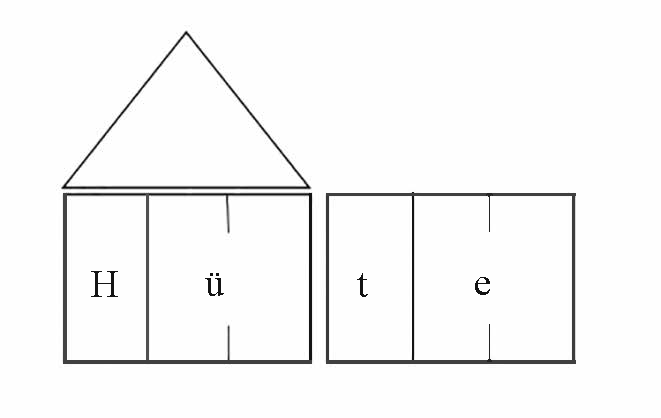
\includegraphics[width=0.5\textwidth]{figures/Huete.pdf}
    \caption{Darstellung der Silbenstruktur des Wortes \textit{Hüte} nach Röber. Die erste Silbe hat einen gespannten Vokal und ist offen.}
    \label{fig:SAMHuetePhon}
\end{figure}

\begin{figure}
    \centering
    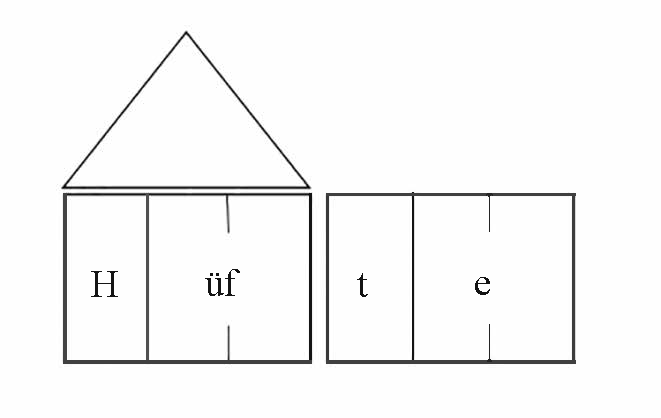
\includegraphics[width=0.5\textwidth]{figures/Huefte.pdf}
    \caption{Darstellung der Silbenstruktur des Wortes \textit{Hüfte} nach Röber. Die erste Silbe hat einen ungespannten Vokal und ist geschlossen.}
    \label{fig:SAMHueftePhon}
\end{figure}

In Abbildung~\ref{fig:SAMHuetePhon} ist das Wort \textit{Hüte} dargestellt. Dieses Wort besteht aus zwei Silben, einer betonten ersten und einer unbetonten zweiten Silbe. Das große Zimmer des Hauses mit Dach ist nur von einem Vokal bewohnt. Abbildung~\ref{fig:SAMHueftePhon} zeigt das Wort \textit{Hüfte}, bei welchem die Koda der ersten Silbe besetzt ist. Der Reim ist nun komplex: zwei Segmente bewohnen das Reim-Zimmer.

Das Häusermodell ist gut geeignet, um den \is{Längenausgleich}Längenausgleich im Reim der betonten Silbe darzustellen: Entweder ist das Reim-Zimmer von einem einzigen Vokal besetzt, dann wird dieser Vokal lang gesprochen (\textit{Hüte}). Oder das Reim-Zimmer ist von einem Vokal und einem Konsonanten bewohnt, dann wird der Vokal kurz gesprochen (\textit{Hüfte}).

Das Modell kann für unterschiedliche Zwecke genutzt werden. Am Anfang des Schriftspracherwerbs dient es dazu, die unterschiedliche Aussprache der Vokalgrapheme zu erklären (Langvokal vs. Kurzvokal). Wenn Lernende nur unter Zuhilfenahme der Phonem-Graphem-Korrespondenzen\footnote{vereinfacht: Zuordnung zwischen Lauten und Schriftzeichen (vgl. Abschnitt~\ref{sec:PGK})} lesen und die Silbenstruktur ignorieren, entstehen oft Produktionen wie \textipa{[\textprimstress hy:\textprimstress te:]} für \textit{Hüte} und \textipa{[\textprimstress hy:f\textprimstress te:]} für \textit{Hüfte} \citep[135]{Roeber2013}. Eine solche Leseaussprache erschwert oder verhindert sogar den lexikalischen Zugriff: Die Kinder erkennen das Wort gar nicht, welches sie gelesen haben, obwohl es ihnen bekannt ist. Besonders hinderlich ist diese Leseaussprache bei Wörtern auf \textit{-er} wie \textit{Winter}. Die Kinder lesen \textipa{[\textprimstress vi:n\textprimstress te:K]} und wissen nicht, was das Wort bedeuten soll.

Mittels des Häusermodells kann man drei Regeln vermitteln, die die Leseaussprache verbessern. Die erste betrifft die Aussprache des Vokals in der betonten Silbe. Ob dieser gespannt, wie in \textit{Hüte}, oder ungespannt, wie in \textit{Hüfte}, gesprochen wird, ist aufgrund des Längenausgleichs im Reim sehr oft aus der Silbenstruktur ableitbar: Wenn das Reim-Zimmer im Haus mit dem Dach ausschließlich einen Vokal enthält, wird der Vokal lang gesprochen. Wenn das Reim-Zimmer außer dem Vokal noch einen Konsonanten enthält, wird der Vokal kurz gesprochen.

Die zweite Regel betrifft die Aussprache der Vokale in der unbetonten Silbe. In unbetonten Silben können keine gespannten Vokale vorkommen. In der Garage gibt es also keine Langvokale. Meist wird der Vokal Schwa gesprochen.

Die dritte Regel betrifft das zu \textipa{[5]} vokalisierte r. Vokalisierte r-Laute treten im Reim einer Silbe auf, wie bei \textit{Winter, wir, Tor}. Ein orthografisches <r> im Reim-Zimmer wird also als tiefes Schwa gesprochen, während ein r im linken Zimmer als \textipa{[K, r]} oder \textipa{[\;R]}  gesprochen wird.

Das Häusermodell hat zahlreiche andere Anwendungsmöglichkeiten, etwa für die Platzierung des Dehnungs-\textit{h}, für die Konsonantenverdopplung beim Silbengelenk und für die Fremdwortschreibung (\cite{Bredel2011} und \cite{Roeber2013}, vgl. Exkurs~\ref{Exkurs:SAM}).


\end{Exkurs}

\subsection{Silbenpräferenzgesetze}\label{subsec:Silbenpräferenz}\is{Silbenpräferenzgesetz}

Beim Spracherwerb kann man beobachten, dass bestimmte Silben sehr früh erworben werden und andere später. Ab einem Alter von 6 Monaten produzieren Kinder sogenannte CV-Silben\is{Silbe!CV} \citep[23]{Falk2008}. Das sind Silben, die aus einem Konsonanten und einem Vokal bestehen, etwa \textipa{[ba]}. Erst mit 10 Monaten kommen CVC-Silben\is{Silbe!CVC} wie \textipa{[bab]} dazu. Auch die ersten Wörter wie \textit{Mama} und \textit{Papa} bestehen aus CV-Silben. Wenn man die Sprachen der Welt betrachtet, kann man feststellen, dass die CV-Silbe in allen Sprachen existiert \citep[213]{Hall2000}, während komplexere Silben wie beispielsweise CCCVCC bei \textit{Strumpf} in vielen Sprachen nicht möglich sind.

Es scheint intuitiv nachvollziehbar, dass Kinder zunächst einfachen Silben wie CV den Vorzug vor komplexeren wie CCCVCC geben.\is{Silbe!VC} Aber warum beginnen sie nicht \zB mit VC-Silben wie \textipa{[ab]}, welche ja genauso einfach sind? Das liegt daran, dass die CV-Silbe einen Sonoritätsverlauf hat, der es sehr einfach macht, die Silbengrenze zu erkennen. Bei einem Wort, das aus CV-Silben besteht, wie \zB \textit{Papa}, steigt die Sonorität in der ersten Silbe vom Onset zum Nukleus hin an. Die zweite Silbe beginnt wieder mit einer niedrigeren Sonorität, sodass dort ein Sonoritätsminimum liegt und die Silbengrenze vor diesem Minimum verortet werden kann.

Ein Wort aus VC-Silben wie \textipa{[am.am]} könnte man anhand der Sonorität allein nicht korrekt silbifizieren. Im Deutschen behilft man sich bei betonten Silben damit, an der Stelle der Silbengrenze einen Knacklaut einzusetzen: \textipa{[Pam.Pam]}.\footnote{Eine Alternative zu \textipa{[Pam.Pam]} wäre \textipa{[Pa\.*mam]} mit dem ersten \textipa{/m/} als Silbengelenk. Damit wäre der Onset der zweiten Silbe jedoch ebenfalls besetzt (vgl. Abschnitt~\ref{subsec:Silbengelenk}).} Der Knacklaut ist ein Obstruent und damit ein niedrigsonoriger Laut. Dadurch wird die Silbengrenze prominent markiert.

Diese in den Sprachen der Welt zu findenden Vorlieben für bestimmte Silben beschreiben \citet[212--217]{Hall2000} und \citet[229--230]{Pompino-Marschall2020} als Silbenpräferenzgesetze.
Man unterscheidet das \textit{Silbenanlautgesetz}, das \textit{Silbenkerngesetz} und das \textit{Silbenauslautgesetz}. 

Laut \is{Silbenpräferenzgesetz!Silbenanlautgesetz}Silbenanlautgesetz haben (in den Sprachen der Welt und im Spracherwerb) präferierte Silben möglichst nur einen Laut im Onset, der möglichst wenig sonor ist. Ein Onset wie \textipa{/p/} ist demnach besser als \textipa{/l/} oder \textipa{/kl/}.

Das \is{Silbenpräferenzgesetz!Silbenkerngesetz}Silbenkerngesetz besagt, dass im Silbenkern Laute mit hoher Sonorität präferiert werden. Ein vokalischer Kern ist also besser als ein sonorantischer, wie er etwa in der zweiten Silbe von \textit{Mantel} nach der Tilgung des Schwa auftritt (vgl. Abschnitt \ref{sec:Schwatilgung}): \textipa{[\textprimstress man.t\s{l}]}.

Laut \is{Silbenpräferenzgesetz!Silbenauslautgesetz}Silbenauslautgesetz sollten in der Koda möglichst wenige Laute stehen, die möglichst sonor sein sollten. Außerdem sollte die Sonorität vom Silbenkern aus abfallen. Eine Silbe mit leerer Koda ist demnach die mit der höchsten Präferenz.


Im Spracherwerb kann man die Wirkung der Silbenpräferenzgesetze gut beobachten. In einem bestimmten Alter vereinfachen Kinder die weniger präferierten CVC-Silben wie bei \textit{Mehl} zu den präferierteren CV-Silben wie \textipa{[me:]} \citep[25]{Falk2008}. Silben mit komplexem Onset wie \textit{krank} \textipa{[\textprimstress kKaNk]} werden zu Silben mit einfachem Onset modifiziert. Dabei wird den wenig sonoren Lauten der Vorzug gegeben. So wird  \textipa{[\textprimstress kKaNk]} zu \textipa{[\textprimstress kaNk]} statt \textipa{[\textprimstress KaNk]} vereinfacht \citep[58]{Muelleretal2018}. Der Onset \textipa{/k/} entspricht dem Silbenanlautgesetz: Er besteht aus einem einzigen, wenig sonoren Laut.

Silbenpräferenzgesetze gelten niemals absolut. Wenn wir aus dem Silbenanlautgesetz ableiten, dass Onsets besetzt sein sollen, dann bedeutet das nicht, dass es keine Silben mit unbesetztem Onset gibt. Es bedeutet lediglich, dass, wenn die Bedingungen das hergeben, der Onset besetzt wird. Für das Standarddeutsche kann man sagen, dass die Silbenpräferenzgesetze dazu führen, dass Onsets betonter Silben immer besetzt sind. Aus dem Silbenkerngesetz kann man ableiten, dass der Silbenkern einer betonten Silbe mit mindestens zwei X-Positionen besetzt sein muss.

\subsection{Silbengelenke}\label{subsec:Silbengelenk}\is{Silbengelenk}

Wie im Abschnitt~\ref{subsec:Sonoritaet} angemerkt, verfügen viele Kinder schon im Vorschulalter über die Kompetenz, Wörter wie \textit{Kinder} oder \textit{Tage} in Silben zu zerlegen. Eine Ausnahme bilden Wörter wie \textit{Messer} oder \textit{Löffel}. Erwachsene sind bei solchen Wörtern mit \is{Doppelkonsonanz}Doppelkonsonanz durch ihre Orthografieerfahrung geneigt zu glauben, die Silbifizierung sei \textit{Mes-ser} und \textit{Löf-fel}. Das würde aber voraussetzen, dass man das \textipa{/s/} bzw. das \textipa{/f/} doppelt spricht. Davon, dass das nicht der Fall ist, kann man sich überzeugen, wenn man Wörter mit Plosiv an der fraglichen Stelle betrachtet, etwa \textit{Hütte}. Wenn man zwei Plosive sprechen würde, müsste man zwei Verschlusslösungen produzieren, wie beim Stottern. 

\citet{Risel2000} zeigt, dass Kinder bei der Silbifizierung dieser Wörter völlig anders vorgehen. Für Zweitklässler zeigt er, dass etwa 60\% der Kinder die Silbengrenze hinter den Vokal setzen: \textit{Me-sser, Lö-ffel}. Etwa 30\% nutzen eine sogenannte Gelenkartikulation mit gedehntem \textipa{/s/} bzw. 
\textipa{/f/} zwischen den Silben: \textipa{[\textprimstress mEs::5]}. Und etwa 10\% setzen die Silbengrenze hinter den fraglichen Konsonanten: \textit{Mess-er, Löff-el}. Erst in der dritten Klasse gibt es zunehmend orthografische Gliederungen nach dem Muster \textit{Mes-ser} und \textit{Löf-fel}.

Warum sind die Antworten der Kinder hier so vielfältig, obwohl sie bei Wörtern ohne Doppelkonsonanz relativ einheitlich sind? Das liegt daran, dass bei Wörtern wie \textit{Messer} und \textit{Löffel} ein \textit{Silbengelenk}\is{Silbengelenk} vorliegt: Ein Konsonant gehört nicht klar zu der einen oder anderen Silbe, sondern er steht zwischen den Silben. Während die \citet[862]{Duden2016} vom Silbengelenk spricht, benutzt \citet[35--36]{Wiese2000} den Terminus \textit{ambisilbischer Konsonant}\is{ambisilbischer Konsonant}. Die neue \citet[862]{Duden2022} verwendet beide Begriffe. Bei einem Wort wie \textit{Messer} steht das \textipa{/s/} also sowohl in der Koda der ersten Silbe als auch im Onset der zweiten. In der Transkription werden ambisilbische Konsonanten durch einen Punkt\is{Silbengrenze} unter dem Konsonanten markiert: \textipa{[\textprimstress mE\.*s5]}.

Wie kommt es dazu, dass ein Konsonant einen solchen Status hat? Um diese Frage zu beantworten schauen wir uns zunächt noch einmal an, welche Bedingungen erfüllt sein müssen, damit eine Silbe betonbar ist (vgl Abschnitt~\ref{subsec:Betonbarkeit}). Eine betonbare Silbe muss eine gewisse Mindestmenge an Material im Reim aufweisen. Entweder muss im Nukleus ein Langvokal stehen, oder ein Diphthong, oder der Nukleus ist mit einem Kurzvokal besetzt, dann darf die Koda aber nicht leer sein. In Abschnitt~\ref{subsec:Reim} hatten wir das formuliert als: Im Reim einer betonten Silbe müssen mindestens zwei X-Positionen besetzt sein. Bei einer Silbe wie \textit{See} stehen diese beiden X-Positionen im Nukleus (vgl. Abbildung~\ref{fig:KonstSee}), bei der Silbe \textit{Bett} steht eine im Nukleus und eine in der Koda, (vgl. Abbildung~\ref{fig:KonstBett}). Bei \textit{Messer} besetzt der Kurzvokal \textipa{/E/} im Nukleus nur eine X-Position. Da die erste Silbe aber betont ist, muss eine weitere X-Position im Reim besetzt sein. Das leistet das \textipa{/s/} in der Koda. 

\begin{figure}
  \centering
  \begin{forest}
      [σ, calign=last
        [Onset, ake
          [X 
          [\textipa{z}]
          ]
        ]
        [Reim, calign=first
          [Nukleus, ake
          [X, name=ERBaum]
    [X [\textipa{e:}]
    {\draw[-] (.north) -- (ERBaum.south);}
    ]
          ]
          [Koda, ake
          ]
        ]
      ]
  \end{forest}
  \caption{Konstituentenanalyse der Silbe \textit{See}. Im Nukleus dieser betonbaren Silbe sind zwei X-Positionen besetzt.}
  \label{fig:KonstSee}
\end{figure}

\begin{figure}
  \centering
 \begin{forest}
      [σ, calign=last
        [Onset, ake
         [X 
          [\textipa{b}]
          ]
        ]
        [Reim, calign=first
          [Nukleus, ake
              [X [\textipa{E}]
            ]
          ]
          [Koda, ake
              [X [\textipa{t}]]
          ]
        ]
      ]
  \end{forest}
  \caption{Konstituentenanalyse der Silbe \textit{Bett}. Im Reim dieser betonbaren Silbe sind zwei X-Positionen besetzt, eine im Nukleus und eine in der Koda.}
  \label{fig:KonstBett}
\end{figure}


\begin{figure}[!htbp]
  \centering
  \begin{forest}
  [Wort
      [σ, calign=last
        [Onset, ake
          [X
          [\textipa{m}]
          ]
        ]
        [Reim, calign=first
          [Nukleus, ake
            [X
            [\textipa{E}]
            ]
          ]
          [Koda, ake, name=ERBaum]
        ]
      ]
      [σ, calign=last
        [Onset, ake
          [X
          [\textipa{\.*s}]
          ]
          {\draw[-] (.north) -- (ERBaum.south);}
        ]
        [Reim
          [Nukleus, ake
            [X
            [\textipa{5}]
            ]
          ]
          [Koda, ake
          ]
        ]
      ]
     ]
  \end{forest}
  \caption{Konstituentenanalyse von \textit{Messer}. \textipa{[s]} ist ein Silbengelenk. Es besetzt gleichzeitig die Koda der ersten Silbe, sodass diese Silbe betonbar wird, und den Onset der zweiten.}
  \label{fig:KonstMesser}
\end{figure}

Nach dem Silbenanlautgesetz ist eine Silbe präferierter, wenn der Onset besetzt ist. Das \textipa{/s/} von \textit{Messer} wird also nicht nur in der Koda der ersten Silbe benötigt, sondern auch, um den Onset der zweiten Silbe zu besetzen (vgl. Abbildung~\ref{fig:KonstMesser}). 

Um die Abgrenzung zwischen ambisilbischen Konsonanten und anderen Konsonanten besser zu verstehen, werden im Folgenden die Wörter \textit{Taste} \textipa{[\textprimstress tas.t@]} (vgl. Abbildung~\ref{fig:KonstTaste}) und \textit{Tasse} \textipa{[\textprimstress ta\.*s@]} (vgl. Abbildung~\ref{fig:KonstTasse2}) verglichen. Bei \textit{Taste} besteht die erste Silbe aus drei Lauten: \textipa{[tas]}. Der erste Konsonant steht im Onset, der Vokal steht im Nukleus und der zweite Konsonant steht in der Koda. Die Silbe ist betonbar, denn zwei X-Positionen im Reim sind besetzt, eine davon im Nukleus, die andere in der Koda. In der zweiten Silbe \textipa{[t@]} steht der Konsonant im Onset und der Vokal im Nukleus. Der Onset ist also besetzt, die Silbe ist eine laut Silbenanlautgesetz präferierte Silbe. Zwar ist im Reim nur eine X-Position besetzt, aber das ist kein Problem, da die Silbe ja nicht betont werden soll.




\begin{figure}[!htbp]
  \centering
  \begin{forest}
  [Wort
      [σ, calign=last
        [Onset, ake
          [X
          [\textipa{t}]
          ]
        ]
        [Reim, calign=first
          [Nukleus, ake
            [X
            [\textipa{a}]
            ]
          ]
          [Koda, ake,
            [X
            [\textipa{s}]
            ]
          ]
        ]
      ]
      [σ, calign=last
        [Onset, ake
          [X
          [\textipa{t}]
          ]
        ]
        [Reim
          [Nukleus, ake
            [X
            [\textipa{@}]
            ]
          ]
          [Koda, ake
          ]
        ]
      ]
     ]
  \end{forest}
  \caption{Konstituentenanalyse von \textit{Taste}. \textipa{[s]} steht in der Koda der ersten Silbe. Es ist kein Silbengelenk, denn der Onset der zweiten Silbe ist durch \textipa{[t]} besetzt.}
  \label{fig:KonstTaste}
\end{figure}

Bei \textit{Tasse} steht das \textipa{[t]} im Onset der ersten Silbe und das \textipa{[a]} im Nukleus (vgl. Abbildung \ref{fig:KonstTasse2}). Überspringen wir für den Moment das \textipa{[s]} und schauen uns die zweite Silbe an. Dort steht noch ein Vokal im Nukleus. Das \textipa{[s]} muss nun zwei Funktionen gleichzeitig erfüllen: Erstens muss eine zweite X-Position im Reim der ersten Silbe besetzt werden, damit die Silbe betonbar wird. Zweitens soll dem Silbenanlautgesetz zufolge nach Möglichkeit der Onset der zweiten Silbe besetzt werden. Für diese beiden Aufgaben gibt es aber nur einen Konsonanten, das \textipa{[s]}. Dieser Konsonant wird also an beiden Stellen gebraucht und wird deshalb zum ambisilbischen Konsonanten. 

\begin{figure}[H]
  \centering
  \begin{forest}
  [Wort
      [σ, calign=last
        [Onset, ake
          [X
          [\textipa{t}]
          ]
        ]
        [Reim, calign=first
          [Nukleus, ake
            [X
            [\textipa{a}]
            ]
          ]
          [Koda, ake, name=ERBaum]
        ]
      ]
      [σ, calign=last
        [Onset, ake
          [X
          [\textipa{\.*s}]
          ]
          {\draw[-] (.north) -- (ERBaum.south);}
        ]
        [Reim
          [Nukleus, ake
            [X
            [\textipa{@}]
            ]
          ]
          [Koda, ake
          ]
        ]
      ]
     ]
  \end{forest}
  \caption{Konstituentenanalyse von \textit{Tasse}. \textipa{[s]} ist ein Silbengelenk. Es besetzt gleichzeitig die Koda der ersten Silbe und den Onset der zweiten.}
  \label{fig:KonstTasse2}
\end{figure}

Ein Silbengelenk kann man als eine Art Notlösung ansehen, wenn nur ein Konsonant vorhanden ist, der aber an zwei Stellen gebraucht wird. Ein Silbengelenk tritt also immer dann auf, wenn drei Bedingungen zusammenfallen:
\begin{itemize}
    \item Eine betonte Silbe geht einer unbetonten voraus.
    \item In der betonten Silbe steht ein Kurzvokal.
    \item Zwischen den beiden vokalischen Kernen steht nur ein Konsonant.
\end{itemize}

Man kann sagen, dass ein Silbengelenk leere Onsets\is{Onset} verhindert. Das bedeutet aber nicht, dass es gar keine leeren Onsets mehr gibt. Wenn zwischen zwei vokalischen Kernen kein Konsonant steht, dann ist der Onset der zweiten Silbe leer, etwa in den Wörtern \textit{Bauer} \textipa{[\textprimstress baU.5]}, \textit{Ehe} \textipa{[\textprimstress Pe:.@]}, \textit{Bio} \textipa{[\textprimstress bi:.o]}. Orthografisch wird der leere Onset in den meisten Fällen durch ein \is{silbentrennendes h}silbentrennendes h gefüllt: \textit{sehen, Mühe, leihen} (vgl. Abschnitt~\ref{AbschnittDehnungsh}). Dieses h wird im Standard aber nicht gesprochen.\footnote{Schon \citet{Levitt1978} stellte jedoch fest, dass Sprecherinnen und Sprecher mit der zunehmenden Alphabetisierung dazu neigen, ihre Aussprache an die Schrift anzupassen. In bestimmten Kontexten, zum Beispiel beim Diktieren, neigen Sprecherinnen und Sprecher deshalb dazu, das silbentrennende h doch mitzusprechen. Auch sind alphabetisierte Personen der Meinung, dass silbentrennende h hören zu können. Im Standard ist es jedoch nicht vorgesehen.} Wenn die Schreibung kein h aufweist, setzen Leseanfänger nicht selten einen Knacklaut als Ersatz ein: \textipa{[\textprimstress bi:.Po]}, was die Worterkennung -- den lexikalischen Zugriff -- erschwert.

Orthografisch werden Silbengelenke oft durch Doppelkonsonanz gekennzeichnet: \textit{Keller, Sonne, Bretter} (vgl. Abschnitt~\ref{sec:Silbengelenksschreibungen}). Aber nicht jede \is{Doppelkonsonanz}Doppelkonsonanz zeigt ein \is{Silbengelenk}Silbengelenk an. Wenn ein Wort aufgrund eines Silbengelenks mit Doppelkonsonanz geschrieben wird, werden alle anderen Wörter der Wortfamilie auch mit Doppelkonsonanz geschrieben, selbst wenn sie kein Silbengelenk haben. So schreibt man \textit{Brett} und \textit{Brettchen} mit <tt>, weil das Silbengelenk in \textit{Bretter} durch <tt> gekennzeichnet wird -- und das, obwohl es weder in \textit{Brett} noch in \textit{Brettchen} ein Silbengelenk gibt.

Auch der umgekehrte Schluss, dass ein Wort ohne Doppelkonsonanz garantiert kein Silbengelenk hat, ist falsch. Komplexe Grapheme\is{Graphem!komplex} wie beispielsweise <sch> und <ch> werden als Silbengelenk nicht verdoppelt: \textit{wischen, machen}. Das Wort \textit{Tasche} beispielsweise ist von der Silbenstruktur her identisch mit \textit{Tasse}, denn das \textipa{/S/} bildet ein Silbengelenk. Trotzdem enthält \textit{Tasche} keine Doppelkonsonanz.

Eine \is{Doppelkonsonanz}Doppelkonsonanz folgt immer einem ungespannten Vokal. Man kann aus einer Doppelkonsonanz deshalb schlussfolgern, dass der vorangehende Vokal ungespannt zu lesen ist. Umgekehrt kann man \textit{nicht} schlussfolgern, dass alle ungespannten Vokale durch Doppelkonsonanz zu kennzeichnen sind, denn sonst müssten Wörter wie \textit{Wald, Ende, Wirt} <Walld, Ennde, Wirrt> geschrieben werden. 

\subsection{Beispielanalysen}

Um eine Konstituentenstrukturanalyse zu erstellen, geht man am besten wie folgt vor: Man transkribiert das zu analysierende Wort und gliedert es in Silben, sucht in jeder Silbe den vokalischen Nukleus und ordnet die Konsonanten vor dem Nukleus dem Onset zu und die Konsonanten, die dem Nukleus innerhalb der Silbe folgen, der Koda. 

Als erstes Beispiel betrachten wir das Wort \textit{streichen}. Zunächst transkribieren wir: \textipa{[\textprimstress StK\t*{aI}.\c{c}@n]}. Eine alternative Transkription mit Schwa-Tilgung wäre \textipa{[\textprimstress StK\t*{aI}.\c{c}\s{n}]}. Wir analysieren zunächst die erste Variante. Die erste Silbe endet nach dem Diphthong. Der Diphthong ist der Nukleus. Alles, was davor steht \newline-- nämlich \textipa{[StK]} -- steht im Onset. Dem Nukleus folgt kein weiterer Konsonant in der ersten Silbe, also ist die Koda leer. In der zweiten Silbe \textipa{[\c{c}@n]} bildet der Schwa-Laut den vokalischen Kern, der Konsonant vor dem Schwa, \textipa{[\c{c}]} steht im Onset, der Konsonant, der dem Schwa folgt, \textipa{[n]}, steht in der Koda. Jedem Konsonanten wird ein X zugeordnet. Dem Diphthong werden zwei X-Positionen zugeordnet, dem Schwa-Laut nur eine. Es ergibt sich die Analyse in Abbildung~\ref{fig:Bspstreichen1}.

\begin{figure}[!htbp]
  \centering
  \begin{forest}
  [Wort
      [σ, calign=last
        [Onset, ake
          [X
          [\textipa{S}]
          ]
          [X
          [\textipa{t}]
          ]
          [X
          [\textipa{K}]
          ]
        ]
        [Reim, calign=first
          [Nukleus, ake
          [X, name=ERBaum]
    [X [\textipa{\t*{aI}}]
    {\draw[-] (.north) -- (ERBaum.south);}
    ]
          ]          
          [Koda, ake,
          ]
        ]
      ]
      [σ, calign=last
        [Onset, ake
          [X
          [\textipa{\c{c}}]
          ]
        ]
        [Reim
          [Nukleus, ake
            [X
            [\textipa{@}]
            ]
          ]
          [Koda, ake
            [X
            [\textipa{n}]
            ]
          ]
        ]
      ]
     ]
  \end{forest}
  \caption{Konstituentenanalyse von \textit{streichen} }
  \label{fig:Bspstreichen1}
\end{figure}

Um eine Konstituentenstrukturanalyse für die zweite Variante \textipa{[\textprimstress StK\t*{aI}.\c{c}\s{n}]} zu erstellen, teilen wir das Wort wieder in Silben ein. Die erste Silbe wird wie in Abbildung~\ref{fig:Bspstreichen1} analysiert. In der zweiten Silbe fehlt der vokalische Kern. Dass wir das Wort trotzdem als zweisilbig wahrnehmen, liegt daran, dass der sonore Laut \textipa{[n]} die Funktion des Vokals übernimmt. \textipa{[n]} erscheint deshalb im Nukleus, siehe Abbildung~\ref{fig:Bspstreichen2}.

\begin{figure}[!htbp]
  \centering
  \begin{forest}
  [Wort
      [σ, calign=last
        [Onset, ake
          [X
          [\textipa{S}]
          ]
          [X
          [\textipa{t}]
          ]
          [X
          [\textipa{K}]
          ]
        ]
        [Reim, calign=first
          [Nukleus, ake
          [X, name=ERBaum]
    [X [\textipa{\t*{aI}}]
    {\draw[-] (.north) -- (ERBaum.south);}
    ]
          ]
          [Koda, ake,
          ]
        ]
      ]
      [σ, calign=last
        [Onset, ake
          [X
          [\textipa{\c{c}}]
          ]
        ]
        [Reim
          [Nukleus, ake
            [X
            [\textipa{\s{n}}]
            ]
          ]
          [Koda, ake
          ]
        ]
      ]
     ]
  \end{forest}
  \caption{Konstituentenanalyse von \textit{streichen} mit getilgtem Schwa. Als sonorer Laut kann das [n] die Funktion des Nukleus übernehmen.}
  \label{fig:Bspstreichen2}
\end{figure}

Schauen wir uns nun ein Wort mit Silbengelenk an: \textit{Kupfer}. Zunächst transkribieren wir: \textipa{[\textprimstress kU\.*{\t{pf}}5]}. Wichtig ist hier, dass wir erkennen, dass \textipa{[\t{pf}]} eine Affrikate ist und damit nur ein einziger Konsonant. Dieser eine Konsonant folgt einem Kurzvokal in einer betonten Silbe. Der Konsonant \textipa{[\t{pf}]} ist darüber hinaus der einzige Konsonant zwischen den beiden vokalischen Kernen des Wortes. Damit ist er ein Silbengelenk.

Der Onset der ersten Silbe ist mit \textipa{[k]} besetzt. Die Affrikate besetzt gleichzeitig die Koda der ersten Silbe und den Onset der zweiten. Die Koda der zweiten Silbe ist leer (vgl. Abbildung~\ref{fig:KonstKupfer}).

\begin{figure}[!htbp]
  \centering
  \begin{forest}
  [Wort
      [σ, calign=last
        [Onset, ake
          [X
          [\textipa{k}]
          ]
        ]
        [Reim, calign=first
          [Nukleus, ake
            [X
            [\textipa{U}]
            ]
          ]
          [Koda, ake, name=ERBaum]
        ]
      ]
      [σ, calign=last
        [Onset, ake
          [X
          [\textipa{\.*{\t{pf}}}]
          ]
          {\draw[-] (.north) -- (ERBaum.south);}
        ]
        [Reim
          [Nukleus, ake
            [X
            [\textipa{5}]
            ]
          ]
          [Koda, ake
          ]
        ]
      ]
     ]
  \end{forest}
  \caption{Konstituentenanalyse von \textit{Kupfer}. \textipa{[\t{pf}]} ist ein Silbengelenk }
  \label{fig:KonstKupfer}
\end{figure}

Als letztes Beispiel sehen wir uns das Wort \textit{Feuer} an. Wir beginnen mit einer Transkription: \textipa{[\textprimstress f\t*{OI}.5]}. Der vokalische Kern der ersten Silbe ist mit \textipa{[\t*{OI}]} besetzt. Im Nukleus der ersten Silbe steht der Konsonant \textipa{[f]}. Die Koda ist leer, denn dem Diphthong folgt kein weiterer Konsonant. Die zweite Silbe besteht nur aus dem vokalischen Kern. Das bedeutete, dass Onset und Koda leer sind. Es ergibt sich die Analyse in Abbildung~\ref{fig:Feuer}.

In Abschnitt~\ref{subsec:Silbenpräferenz} hatten wir diskutiert, dass es eine Tendenz in den Sprachen der Welt gibt, leere Onsets zu vermeiden, damit die Silbengrenze erkennbar ist. Im bundesdeutschen Standard ist es sogar so, dass bei leeren Onsets in betonten Silben eine Art Notbesetzung mit dem Knacklaut erfolgt. Bei unbetonten Silben erfolgt diese Knacklautepenthese jedoch nicht. Der Onset der 2. Silbe von \textit{Feuer} ist deshalb unbesetzt.

\begin{figure}[!htbp]
  \centering
  \begin{forest}
  [Wort
      [σ, calign=last
        [Onset, ake
          [X
          [\textipa{f}]
          ]
        ]
        [Reim, calign=first
         [Nukleus, ake
          [X, name=ERBaum]
    [X [\textipa{\t*{OI}}]
    {\draw[-] (.north) -- (ERBaum.south);}
    ]
          ]
          [Koda, ake,
          ]
        ]
      ]
      [σ, calign=last
        [Onset, ake
        ]
        [Reim
          [Nukleus, ake
            [X
            [\textipa{5}]
            ]
          ]
          [Koda, ake
          ]
        ]
      ]
     ]
  \end{forest}
  \caption{Konstituentenanalyse von \textit{Feuer}. Der Onset der zweiten Silbe ist leer.}
  \label{fig:Feuer}
\end{figure}



\section{Phonologische Prozesse}\label{section:phonProzesse}\is{phonologischer Prozess}

In Kapitel~\ref{kap:Phonetik} wurde vielfach gezeigt, dass die Schreibung im Deutschen regelhaft von der Lautung abweicht. Beispielsweise schreibt man \textit{Tag} mit <g>, obwohl man \textipa{[ta:k]} mit \textipa{[k]} spricht.

In der Schule lernt man dazu, dass verwandte Wörter gleich geschrieben werden. Da es zum Beispiel \textit{Tage} und \textit{Tagesform} gibt, und diese mit \textipa{[g]} gesprochen und folglich mit <g> geschrieben werden, schreibt man eben auch \textit{Tag}. Dagegen kann man einwenden, dass man dann genauso gut die Lautung von \textit{Tag} auf die abgeleiteten Formen übertragen könnte und also <*Tak>, <*Take> und <*Takesform> schreiben könnte. Es gibt aber gute Gründe dafür, nicht so verfahren. Die Schreibung orientiert sich nämlich an einer zugrundeliegenden\footnote{\textit{Zugrundeliegend} bedeutet, dass diese Form im mentalen Lexikon gespeichert ist und die Grundlage für alle Verwendungen bildet.} sogenannten \textit{phonologischen Repräsentation}\is{phonologische Repräsentation} -- für \textit{Tag} wäre diese \textipa{/ta:g/} -- aus welcher die Lautung \textipa{[ta:k]} regelhaft abgeleitet wird \citep[62--65]{Ramers1998}.

Eine phonologische Repräsentation ist im mentalen Lexikon\is{mentales Lexikon} der Sprecherinnen und Sprecher gespeichert. Wenn man ein Wort verwenden möchte, greift man zunächst auf diese phonologische Repräsentation zu. Über Ausspracheregeln, die sogenannten \textit{phonologischen Prozesse}\is{phonologischer Prozess} verändert man die phonologische Repräsentation und gewinnt dabei eine \textit{phonetische Repräsentation}\is{phonetische Repräsentation}, die die Grundlage für die tatsächliche Äußerung bildet. Dieser Vorgang ist in Abbildung~\ref{fig:phonproz} für das Wort \textit{Tag} dargestellt. Der phonologische Prozess, der bei diesem Wort angewandt wird, heißt \textit{Auslautverhärtung}. Die \isi{Auslautverhärtung} führt dazu, dass das zugrundeliegende \textipa{/g/} als \textipa{[k]} gesprochen wird.

\begin{figure}
    \centering
    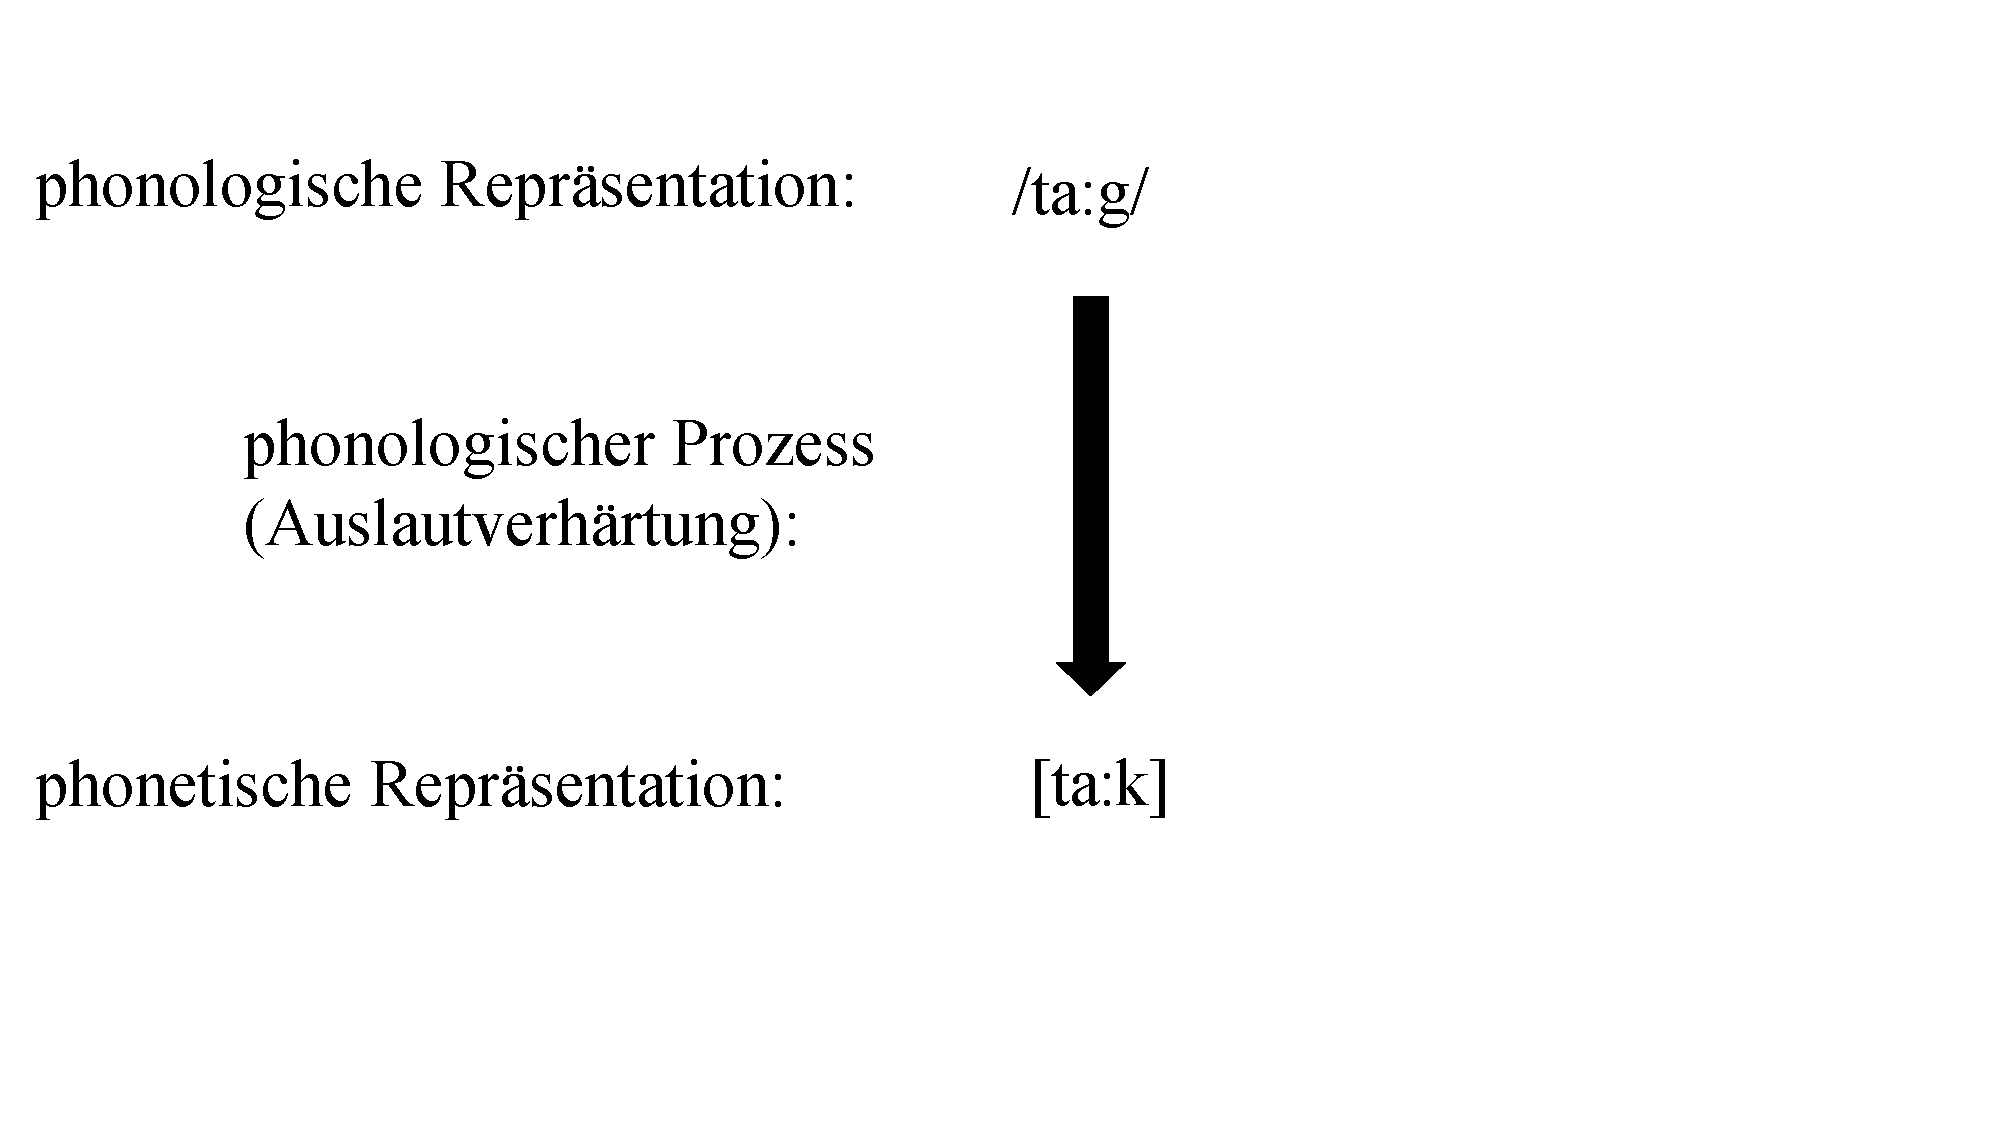
\includegraphics[width=0.5\textwidth]{figures/auslautv.pdf}
    \caption{Wirkung eines phonologischen Prozesses am Beispiel \textit{Tag}\label{fig:phonproz}}
\end{figure}


Wie kommt man zur Annahme einer phonologischen Repräsentation? Wa\-rum geht man nicht einfach davon aus, dass die Singularform \textipa{[ta:k]} genauso im mentalen Lexikon vorhanden ist, und dass als Basis für die Pluralbildung eben die andere Form \textipa{/ta:g/} gespeichert ist? Als Indiz dafür, dass es die phonologische Repräsentation \textipa{/ta:g/} tatsächlich gibt, kann man  Spontanbildungen\is{Spontanbildung} heranziehen. Wenn man mit \textit{Tag} ein neues Wort bilden möchte, etwa mittels eines Adjektivsuffix \textit{-ig} wie in \textit{eklig} oder \textit{-isch} wie in \textit{kindisch} oder mittels des Verbalisierers \textit{-ieren} wie in \textit{telefonieren}, dann wären die resultierenden Formen \textit{tagig, tagisch} und \textit{tagieren}. Alle diese Wörter würden mit \textipa{[g]} gesprochen werden. Es ist nicht möglich, dass Sprecherinnen und Sprecher die Information, genau bei diesen Verbindungen \textipa{[g]} und nicht \textipa{[k]} zu benutzen, irgendwann mal in ihr \is{mentales Lexikon}mentales Lexikon aufgenommen haben, denn sie haben diese Wörter noch nie gehört, sondern gerade spontan gebildet.

Eine \is{phonologische Repräsentation}phonologische Repräsentation enthält laut \citet[63]{Ramers1998} nur die Informationen, die nicht regelhaft vorhersagbar sind. Wie im folgenden Abschnitt~\ref{sec:Auslautverhaertung} genauer ausgeführt wird, gibt es im Deutschen keine stimmhaften Obstruenten in der Koda einer Silbe. Eine Produktion wie \textipa{[ta:g]} ist im Deutschen deshalb nicht möglich. Es werden also regelhaft alle stimmhaften Obstruenten in der Koda entstimmt, sodass diese Information nicht in der phonologischen Repräsentation gespeichert werden muss.


Da \is{Transkription!Klammern}\is{Transkription!Schrägstriche}phonologische Repräsentationen Ab\-straktionen sind, also nicht produziert werden, werden sie wie Phoneme in \is{Transkription!Schrägstriche}Schrägstrichen notiert. Phonetische Repräsentationen sind die Grundlage für Produktionen und werden deshalb wie Phone in eckigen Klammern notiert (vgl. Abbildung~\ref{fig:phonproz})\is{Transkription!Klammern}.

Phonologische Prozesse sind sprachspezifisch. Es wird zum Beispiel nicht in jeder Sprache auslautverhärtet. Beim Erlernen einer Fremdsprache können Sprecherinnen und Sprecher sich zu Beginn nicht (oder nicht sofort) von den phonologischen Prozessen ihrer Erstsprache lösen. Das führt zu einem sprachspezifischen Akzent. Zum Beispiel ist es deutschen Muttersprachlern beim Erlernen des Englischen zu Beginn fast unmöglich, die Wörter \textit{bad} und \textit{bat} erkennbar unterschiedlich zu produzieren, weil sie bei \textit{bad} auslautverhärten.


\begin{Definition}{Phonologische Prozesse}\is{phonologischer Prozess}

\noindent Phonologische Prozesse sind sprachspezifische Ausspracheregeln, die phonologische Repräsentationen in Abhängigkeit vom Kontext in phonetische Repräsentationen überführen.

\end{Definition}


\subsection{Auslautverhärtung}\label{sec:Auslautverhaertung}\is{Auslautverhärtung}

Als erster phonologischer Prozess wird hier die schon erwähnte Auslautverhärtung betrachtet. Bei der Auslautverhärtung werden bestimmte in der phonologischen Repräsentation vorhandene stimmhafte Laute unter bestimmten Bedingungen stimmlos. Es sind also nicht alle stimmhaften Laute betroffen. Beispielsweise wird das \textipa{/d/} bei \textit{danke} nicht stimmlos und das \textipa{/m/} von \textit{Helm} auch nicht. Die Regel der Auslautverhärtung wird deshalb im Folgenden präzisiert. 

Die Auslautverhärtung betrifft im deutschen Standard Obstruenten\is{Obstruent}, also Plosive und Frikative (vgl. Abschnitt~\ref{sec:ObstSon}). Man spricht \textit{Bild} \textipa{[bIlt]}, \textit{schrieb} \textipa{[SKi:p]}, \textit{lag} \textipa{[la:k]}, \textit{brav} \textipa{[bKa:f]} (obwohl die flektierte Form \textit{brave} mit \textipa{[v]} gesprochen wird) und \textit{Gras} \textipa{[gKa:s]} (obwohl bei \textit{Gräser} \textipa{[z]} gesprochen wird). Sonoranten\is{Sonorant} sind von der Auslautverhärtung nicht betroffen. 

In Teilen Süddeutschlands, der Schweiz und Österreich führt die Auslautverhärtung -- anders als im Norddeutschen -- nicht dazu, dass Wörter wie \textit{bunt} und \textit{Bund} identisch klingen. Die Sprecherinnen und Sprecher unterscheiden \textit{Bund} und \textit{bunt} akustisch dadurch, dass der finale Konsonant in \textit{Bund} kürzer und der Vokal vor dem Konsonanten länger als in \textit{bunt} ist \citep[72]{DudenAussprache2023}.

Im norddeutschen Sprachraum wirkt sich die Auslautverhärtung, wie \citet[242]{Hall2000} zeigt, auf Obstruenten \textit{in der Koda einer Silbe} aus. Die Auslautverhärtung gibt es also wortfinal wie in den Beispielen oben, aber auch silbenfinal wie bei \textit{Erbse} \textipa{[\textprimstress PE5p.z@]}, \textit{Schreibtisch} \textipa{[\textprimstress SK\t*{aI}p.tIS]}, \textit{täglich} \textipa{[\textprimstress te:k.lI\c{c}]} oder sogar als nichtfinaler Konsonant in der Koda, etwa bei \textit{Jagd} \textipa{[ja:kt]}, wo die letzten beiden Konsonanten betroffen sind, oder \textit{lobt} \textipa{[lo:pt]}, wo der letzte Konsonant schon stimmlos ist, der vorletzte aber durch die Auslautverhärtung entstimmt wird.


\begin{Definition}{Auslautverhärtung}\is{Auslautverhärtung}

\noindent Die Auslautverhärtung ist ein \isi{phonologischer Prozess}, durch welchen zugrundeliegende stimmhafte Obstruenten in der \is{Koda}Koda einer Silbe stimmlos werden.

\end{Definition}


Die Auslautverhärtung ist im norddeutschen Standard ein obligatorischer Prozess\is{phonologischer Prozess! obligatorisch}. Das bedeutet, dass Sprecherinnen und Sprecher nicht wählen können, ob sie die Auslautverhärtung durchführen oder nicht.

Wie alle phonologischen Prozesse ist auch die Auslautverhärtung sprachspezifisch. Im Russischen und Türkischen wird ebenfalls auslautverhärtet. Im Englischen und Französischen wird jedoch nicht auslautverhärtet (vgl. Beispiele (\ref{EnglischAuslaute}) bis (\ref{RussischAuslautverhaertung}) auf Seite \pageref{EnglischAuslaute} in Kapitel~\ref{kap:Graphematik}).


\subsection{Epenthese}\label{sec:Epenthese}\is{Epenthese}

Unter einer Epenthese versteht man die Einfügung eines Segments, etwa wenn Sprecherinnen und Sprecher das Wort \textit{Hemd} \textipa{[hEmpt]} statt \textipa{[hEmt]} sprechen. Die Einfügung von \textipa{[p]} entsteht hier durch eine zeitliche Verschiebung der Bewegungen von Velum, Lippen und Zungenspitze. Um vom \textipa{[m]} zum \textipa{[t]} überzugehen, muss das Velum angehoben und die Lippen müssen geöffnet werden. Vor der Öffnung der Lippen muss jedoch der alveolare Verschluss für \textipa{[t]} produziert werden. Wenn das Velum angehoben wird und die Lippen geöffnet werden, der alveolare Verschluss aber noch nicht gebildet wurde, entsteht ein bilabialer Plosiv. Andere Beispiele für Epenthesen sind die Einsetzung\is{phonologischer Prozess!fakultativ} von \textipa{[p]} bei \textipa{[kOmpt]} für \textit{kommt} oder die \textipa{[t]}-Epenthese beim Genitiv von \textit{Leben, Lebens} \textipa{[\textprimstress le:b@nts]}.

Während die bisher angesprochenen Epenthesen fakultativ sind, ist die \is{Knacklaut-Epenthese}Knacklaut-Epenthese im Standard obligatorisch. Der Knacklaut \textipa{[P]} wird \citet[65]{Hall2000} zufolge im Onset einer Silbe platziert, wenn

\begin{itemize}
    \item dort kein weiteres Segment steht \textit{und}
    \item die Silbe betont ist oder wenn es sich um die erste Silbe eines Wortes handelt (vgl. Abschnitt~\ref{subsection:Plosive}).
\end{itemize}

Die \is{phonologische Repräsentation}phonologische Repräsentation des Wortes \textit{Amt} ist also \textipa{/amt/}. Über die Knacklaut-Epenthese kommt man zur \is{phonetische Repräsentation}phonetischen Repräsentation \textipa{[Pamt]}, denn der Onset der ersten (und einzigen) Silbe des Wortes ist leer. Bei \textit{Beamte} wird der Knacklaut am Anfang der zweiten Silbe eingesetzt, denn diese Silbe ist betont und ihr Onset wäre sonst leer. Die phonologische Repräsentation ist also \textipa{/b@\textprimstress am.t@/}, die phonetische ist \textipa{[b@\textprimstress Pam.t@]}.\footnote{Bei \textit{bauen} wird hingegen kein Knacklaut eingesetzt, obwohl die zweite Silbe einen leeren Onset hat. Das liegt daran, dass diese Silbe unbetont ist.}




\subsection{\textipa{/K/}-Vokalisierung}\is{R-Vokalisierung@\textipa{/K/}-Vokalisierung}
\label{subsec:r-Vokalisierung}

Bei der \textipa{/K/}-Vokalisierung wird ein \textipa{/K/}, welches in der Koda einer Silbe steht, zum tiefen Schwa \textipa{[5]}. Wir schauen uns dazu das Wort \textit{Tier} mit seiner Pluralform \textit{Tiere} an. Die phonologische Repräsentation\is{phonologische Repräsentation} von \textit{Tier} ist \textipa{/ti:K/}. Die Silbenstruktur der phonologischen Repräsentation von \textit{Tier} ist in Abbildung~\ref{Silbenstruktur_Tier} darstellt. Das \textipa{/K/} steht hier in der Koda und wird deshalb vokalisiert. Es entsteht die phonetische Repräsentation\is{phonetische Repräsentation} \textipa{[ti:5]} oder auch als Diphthong \textipa{[t\t*{i5}]}, die in Abbildung~\ref{Silbenstruktur_Tier_vokalisiert} dargestellt ist. Das tiefe Schwa ist jetzt Bestandteil des Nukleus.\footnote{Phonologisch betrachtet müsste man für den ursprünglichen Nukleus \textipa{/i:/} zwei X-Positionen vorsehen, sodass insgesamt drei X-Positionen im Nukleus stehen. Phonetisch betrachtet bildet das \textipa{/i:/} aber nun mit dem tiefen Schwa zusammen einen Diphthong. Diphthonge besetzen zusammen nur zwei X-Positionen.}

\begin{figure}[!htbp]
  \centering
  \begin{forest}
[σ 
        [Onset, ake 
          [X [\textipa{t}]]
        ]
       [Reim 
         [Nukleus 
           [X, name=ERBaum]
           [X
                [\textipa{i:}]
                {\draw[-] (.north) -- (ERBaum.south);}
            ]
        ] 
          [Koda, ake
            [X [\textipa{K}]]
          ]
      ] 
] 
  \end{forest}
  \caption{Konstituentenanalyse der phonologischen Repräsentation von \textit{Tier}: Der r-Laut steht in der Koda.}
  \label{Silbenstruktur_Tier}
\end{figure}

Bei der Pluralform \textit{Tiere} wird, wie in Abbildung~\ref{Silbenstruktur_Tiere} dargestellt, nicht vokalisiert, weil das \textipa{/K/} nicht in der Koda, sondern im Onset steht.

\begin{figure}[!htbp]
  \centering
  \begin{forest}
[σ 
        [Onset, ake 
          [X [\textipa{t}]]
        ]
        [Reim 
         [Nukleus
           [X
                [\textipa{i}]
            ]
            [X
                [\textipa{5}]
            ]
        ] 
          [Koda, ake
          ] 
      ] 
] 
  \end{forest}
  \caption{Konstituentenanalyse von \textit{Tier} mit Vokalisierung. Der vokalisierte r-Laut (tiefes Schwa) steht im Nukleus. \label{Silbenstruktur_Tier_vokalisiert}}
\end{figure}



\begin{figure}[!htbp]
  \centering
  \begin{forest}
  [Wort
      [σ, calign=last
        [Onset, ake
          [X [\textipa{t}]]
        ]
      [Reim, calign=first
          [Nukleus, ake
          [X, name=ERBaum]
    [X [\textipa{i:}]
    {\draw[-] (.north) -- (ERBaum.south);}
    ]
          ]
          [Koda,
      ]
      ]
      ]
      [σ, calign=last
      [Onset, ake
          [X [\textipa{K}]]
        ]
        [Reim
          [Nukleus, ake
            [X [\textipa{@}]]
          ]
          [Koda
          ]
        ]
      ]
    ]
  \end{forest}
  \caption{Konstituentenanalyse von \textit{Tiere}: Der r-Laut steht im Onset der zweiten Silbe und wird nicht vokalisiert.}
  \label{Silbenstruktur_Tiere}
\end{figure}

Die \textipa{/K/}-Vokalisierung ist \citet[144]{Noske1993} zufolge obligatorisch nach gespannten Vokalen, \zB in \textit{wir, Ohr, wer}, und fakultativ nach ungespannten, \zB in \textit{wirr, Ort, werfen}. Laut \citet[856f]{Duden2022} jedoch wird jedes \textipa{/K/} in der Koda vokalisiert, also auch nach ungespannten Vokalen wie in \textit{wirr, Herr, dürr} \textipa{[vI5, hE5, dY5]}. Das \citet{DudenAussprache2023} wiederum sieht nach ungespanntem Vokal keine \textipa{/K/}-Vokalisierung vor: \textipa{[vIr, hEr, dYr]}. Das \citet[140]{DudenZweifelsfaelle2021} empfiehlt ebenfalls, nach ungespannten Vokalen auf die \textipa{/K/}-Vokalisierung zu verzichten. 

Unterschiedliche Arten der Realisierung gibt es außerdem nach \textipa{/a/}. Während die \citet[857]{Duden2022} auch dort eine Vokalisierung vorsieht, \zB bei \textit{Star} \textipa{[Sta:5]} und \textit{starr} \textipa{[Sta5]}, gibt das \citet[819]{DudenAussprache2023} \textipa{[Sta:]} und \textipa{[Star]} an.


\subsection{Schwa-Tilgung}\label{sec:Schwatilgung}\is{Schwa-Tilgung}

Der \is{Laute!Schwa}Schwa-Laut \textipa{/@/} ist \citet[106]{KoherlRodgers2001} zufolge der häufigste Vokal im Deutschen. Er tritt ausschließlich in unbetonten Silben auf. Durch das im Deutschen vorherrschende \is{Trochäus}trochäische Betonungsmuster findet man ihn meist in der Silbe, die der betonten Silbe folgt, etwa in \textit{Mantel} \textipa{/\textprimstress man.t@l/}, \textit{bitten} \textipa{/\textprimstress bI\.*{t}@n/}, \textit{müssen} \textipa{/\textprimstress mY\.*{s}@n/}, \textit{rasen} \textipa{/\textprimstress ra:.z@n/}, \textit{malen} \textipa{/\textprimstress ma:.l@n/}, \textit{mahnen} \textipa{/\textprimstress ma:.n@n/}, \textit{bauen} \textipa{/baU.@n/}, \textit{ihrem} \textipa{/\textprimstress i:.K@m/}. Aber auch in Wörtern mit \is{Präfix}Präfix, etwa in \textit{gelingen} \textipa{/g@\textprimstress lI\.*N@n/}, \textit{besichtigen} \textipa{/b@\textprimstress zI\c{c}.tig@n/} usw. tritt er auf.

Prinzipiell kann das Schwa in der Standardlautung getilgt werden (d.\,h. entfallen), wenn der Folgekonsonant ein Sonorant ist \citep[41ff]{DudenAussprache2023}. Dieser Sonorant wird dabei silbisch\is{Transkription!silbischer Konsonant}, er übernimmt also die Funktion des Nukleus. \is{Transkription!silbischer Konsonant}In der Transkription kennzeichnet man das durch einen kleinen Strich unter dem Konsonanten. Bei \textit{Mantel} wird aus der phonologischen Repräsentation \textipa{/\textprimstress man.t@l/} durch die Schwa-Tilgung die phonetische Repräsentation \textipa{[\textprimstress man.t\s{l}]} mit silbischem \textipa{[l]}. Weitere Beispiele für Schwa-Tilgungen sind \textit{bitten} \textipa{[\textprimstress bI\.*{t}\s{n}]}, \textit{müssen} \textipa{[\textprimstress mY\.*{s}\s{n}]} , \textit{rasen} \textipa{[\textprimstress ra:.z\s{n}]}, \textit{malen} \textipa{[\textprimstress ma:.l\s{n}]}, \textit{mahnen} \textipa{[\textprimstress ma:.n\s{n}]}, \textit{bauen} \textipa{[\textprimstress baU.\s{n}]}, \textit{ihrem} \textipa{[\textprimstress Pi:.K\s{m}]} (oft mit Resilbifizierung und \textipa{/K/}-Vokalisierung: \textipa{[Pi:5m]}).

Wenn der Folgelaut kein Sonorant ist, erfolgt keine Schwa-Tilgung: \textit{bittet} \textipa{[\textprimstress bI\.*{t}@t]}, nicht: \textipa{[\textprimstress bIt.t]}, \textit{ratloses} \textipa{[\textprimstress Ka:t.lo.z@s]}, nicht: \textipa{[\textprimstress Ka:t.lo.zs]}.

Die \is{Schwa-Tilgung}Schwa-Tilgung ist immer optional. Ob ein Schwa vor Sonorant wirklich getilgt wird, hängt nicht nur vom Folgelaut, sondern auch vom Register,\footnote{Unter \textit{Register} versteht man den Sprachgebrauch, der für eine bestimmte Kommunikationssituation charakteristisch ist, etwa Kommunikation  mit Kindern, Kommunikation in formellen Situationen usw. \citep{Halliday1978}.}\is{Register} vom Sprechtempo, vom vorangehenden Laut und der Position der Schwa-Silbe ab. \citet[101]{KoherlRodgers2001} zeigen für norddeutsche Sprecherinnen und Sprecher, dass die Schwa-Tilgung in Spontansprache häufiger ist als in gelesener Sprache. Während in gelesener Sprache 44\% von allen Schwas getilgt wurden, wurden in spontaner Sprache 64\% getilgt \citep[104]{KoherlRodgers2001}. Außerdem wird das Schwa häufiger nach Nasalen, Liquiden und Vokalen getilgt als nach Frikativen. Man kann also eher eine Tilgung bei Wörter wie \textit{mahnen, malen, bauen} erwarten als in Wörtern wie \textit{rasen, müssen}. Wenn die Silbe mit dem Schwa der betonten Silbe vorangeht (zum Beispiel in \textit{gelingen}) wird das Schwa seltener getilgt, als wenn die Silbe mit dem Schwa der betonten Silbe folgt.


\subsection{Assimilation}\label{subsection:Assimilation}\is{Assimilation}

Bei der Assimilation beeinflusst ein Laut einen benachbarten so, dass der beeinflusste Laut sich in einer oder mehreren Merkmalen an den beeinflussenden Laut angleicht \citep[89]{Hall2000}. Abbildung~\ref{fig:regNasalass} stellt eine Assimilation beim  Wort \textit{Rennbahn} dar. Die phonologische Repräsentation ist \textipa{/\textprimstress KEn\textsecstress ba:n/}. Über die Assimilation kann daraus in spontanter Sprache \textipa{[\textprimstress KEm\textsecstress ba:n]} werden \citep{Zimmereretal:2009}.\is{Nasalassimilation}

\begin{figure}
    \centering
    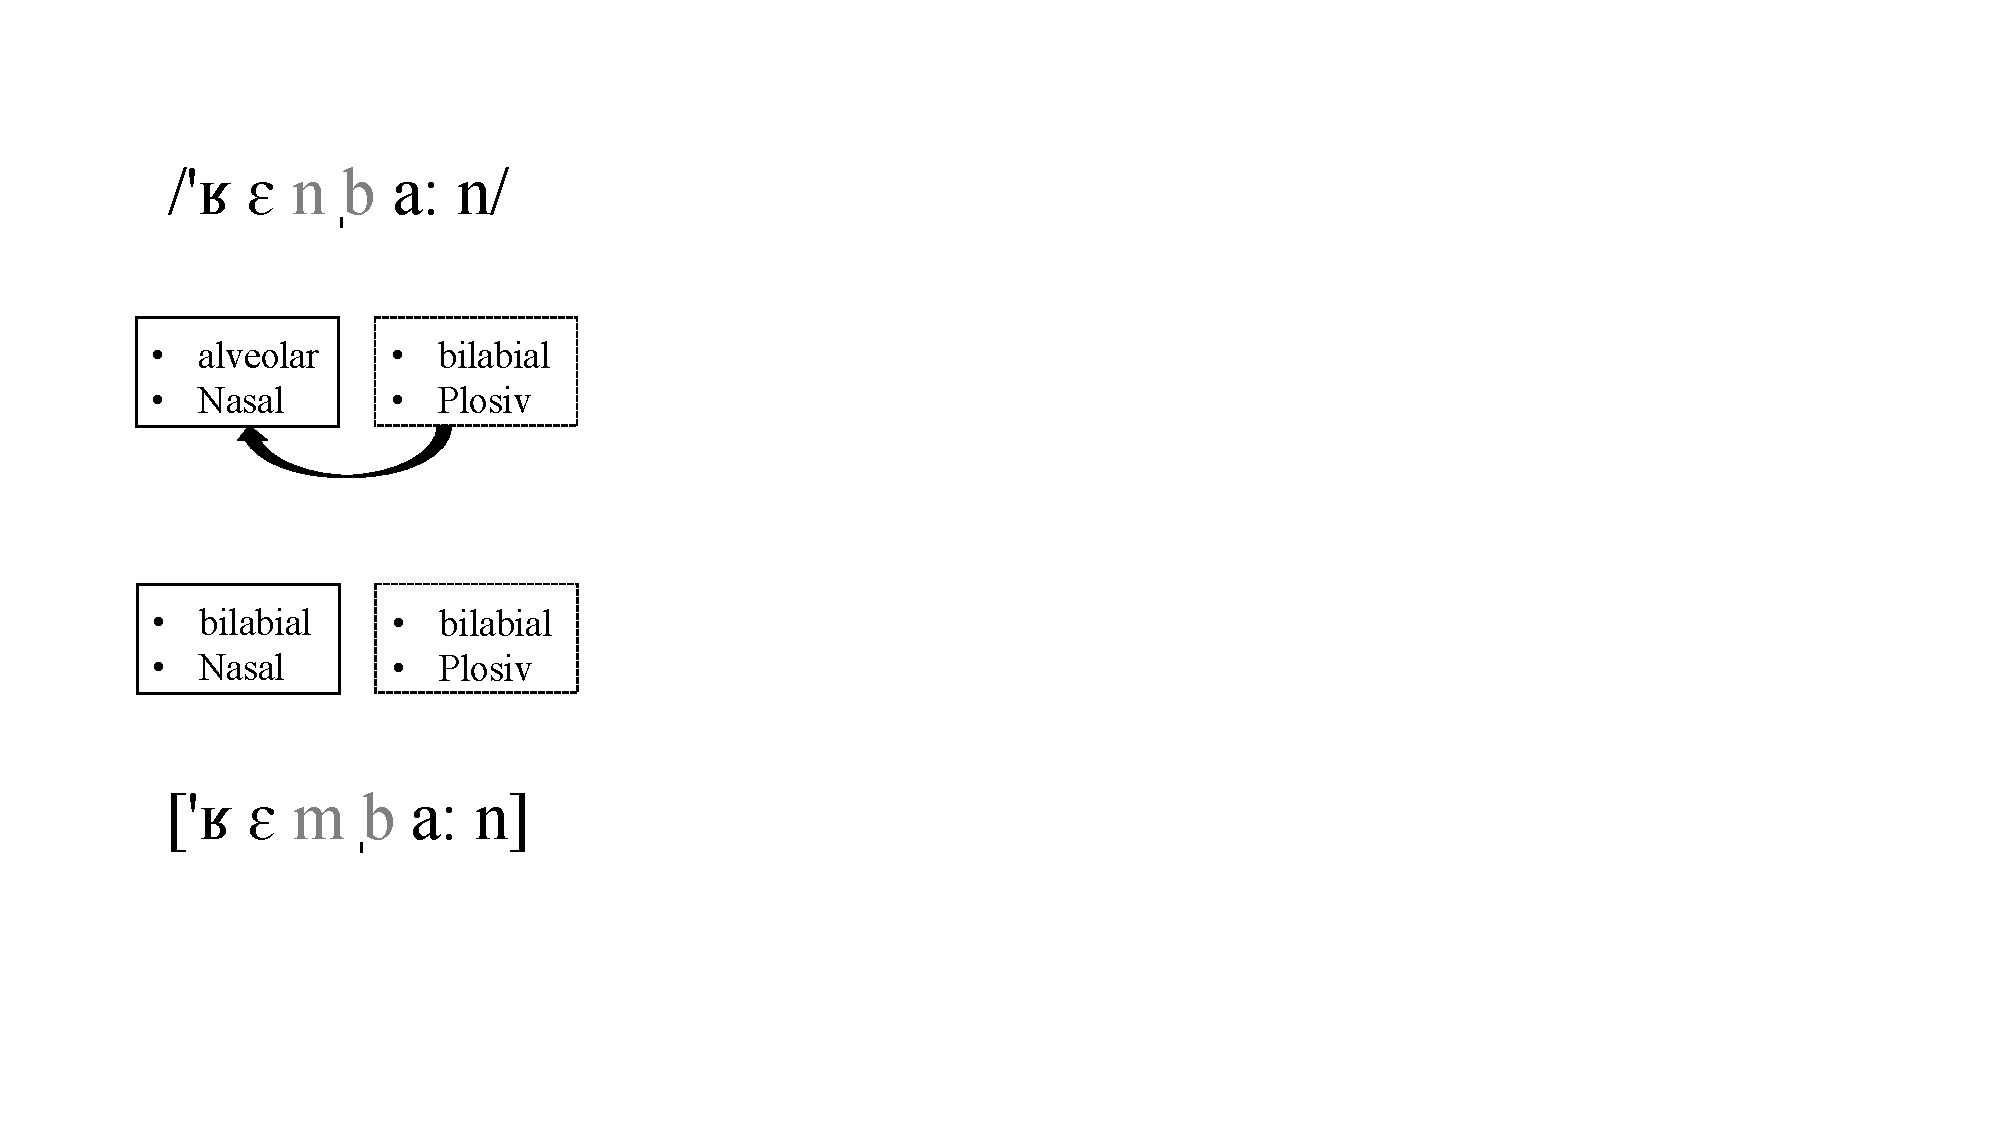
\includegraphics[width=0.4\textwidth]{figures/assimilation.pdf}
    \caption{Regressive Nasalassimilation \label{fig:regNasalass}}
\end{figure}

Der beeinflusste Laut, das \textipa{/n/} in der \is{phonologische Repräsentation}phonologischen Repräsentation, ist ein alveolarer Nasal (oberes linkes Kästchen in der Abbildung). Der beeinflussende Laut, das \textipa{/b/}, ist ein bilabialer Plosiv (oberes rechtes Kästchen in der Abbildung). Der Plosiv überträgt seinen Artikulationsort \textit{bilabial} auf den Nasal, sodass dieser zum bilabialen Nasal \textipa{[m]} wird (unteres linkes Kästchen).

Eine\is{Assimilation!regressiv}\is{Assimilation!progressiv} Assimilation wie bei \textipa{/nb/} zu \textipa{[mb]}, bei der der Folgelaut den vorangehenden beeinflusst, nennt man \textit{regressive Assimilation} (auch \textit{anticipatory assimilation}). Bei einer \textit{progressiven Assimilation} (auch \textit{carry over assimilation}) beeinflusst der vorangehende Laut den folgenden. Progressive Assimilationen kommen häufig nach einer Schwa-Tilgung vor, etwa bei dem Wort \textit{haben}. Die phonologische Repräsentation ist \textipa{/\textprimstress ha:.b@n/}. Dann kann eine Schwa-Tilgung erfolgen, sodass \textipa{[\textprimstress ha:.b\s{n}]} entsteht. Erst dann kann assimiliert werden, indem das \textipa{/b/} seinen Artikulationsort auf das \textipa{/n/} überträgt, sodass \textipa{[\textprimstress ha:.b\s{m}]} entsteht. Laut \citet[69f]{DudenAussprache2023} treten progressive Assimilationen wie in \textipa{[\textprimstress ha:b\s{m}]} im Standarddeutschen auf, sie sind aber nicht obligatorisch.

Weitere Beispiele für die Nasalassimilation diskutiert \citet[Kap. 4]{Hall1992}. Einige davon sind in Tabelle~\ref{tab:Assimilation} wiedergegeben. Bei \textit{Becken} (erstes Beispiel in der Tabelle) wird zunächst der Schwa-Laut getilgt: \textipa{[\textprimstress bE\.*{k}\s{n}]}. Dann erfolgt eine progressive Assimilation. Der velare Plosiv überträgt sein Ortsmerkmal auf den ursprünglich alveolaren Nasal. Es entsteht die phonetische Repräsentation \textipa{[\textprimstress bE\.*k\s{N}]}. Das Beispiel \textit{legen} ist vergleichbar. Zunächst wird das Schwa getilgt, dann überträgt das \textipa{/g/} sein Ortsmerkmal auf den Nasal.

Von einer Assimilation spricht man auch, wenn ein Merkmal nur teilweise übertragen wurde, wie etwa bei \textit{Senf} (drittes Beispiel in der Tabelle). Hier ist der beeinflussende Laut, das \textipa{/f/}, ein labiodentaler Laut. Durch die Assimilation wird der vorangehende Laut \textipa{/n/} nicht notwendigerweise labiodental, aber zumindest labial. Anschließend kann eine Epenthese erfolgen, sodass die phonetische Repräsentation \textipa{[zEmpf]} entsteht.

Bei \textit{Angriff} (viertes Beispiel) erfolgen eine \textipa{[P]}-Epenthese und eine regressive Assimilation. Das \textipa{/g/} überträgt sein Ortsmerkmal auf den vorangehenden Nasal. Im Unterschied zum ersten bis dritten Beispiel in der Tabelle, wo der erste Prozess erst die Voraussetzungen für den zweiten Prozess schafft, sind die beiden Prozesse beim vierten Beispiel unabhängig voneinander. Man kann also genauso gut annehmen, dass zuerst die Assimilation und dann die \textipa{[P]}-Epenthese erfolgt.

\footnotesize
\begin{table}
\centering
\caption{Beispiele für Assimilationsprozesse im Deutschen in Kombination mit anderen phonologischen Prozessen\label{tab:Assimilation}}
\begin{tabular}{lllll}\lsptoprule
Orthograf. & Phonolog.&1. Phonolog. & 2. Phonolog. & Phonet. \\
Form & Repräs.& Prozess & Prozess & Repräs.\\\midrule
\textit{Becken} & \textipa{/\textprimstress bE\.*k@n/} & Schwa-Tilgung & prog. Assim. & \textipa{[\textprimstress bE\.*k\s{N}]}\\
\textit{legen} & \textipa{/\textprimstress le:.g@n/} & Schwa-Tilgung & prog. Assim. & \textipa{[\textprimstress le:.g\s{N}]}\\
\textit{Senf} & \textipa{/zEnf/} & reg. Assim. & Epenthese&  \textipa{[zEmpf]}\\
\textit{Angriff} & \textipa{/\textprimstress an.gKIf/} & \textipa{[P]}-Epenthese & reg. Assim. & \textipa{[\textprimstress PaN.gKIf]}\\
\lspbottomrule
\end{tabular}
\end{table}

\normalsize

Auch die \isi{Stimmhaftigkeit} kann assimiliert werden, beispielsweise wenn auf stimmlose Plosive ein Liquid folgt wie bei \textit{Kleid} oder \textit{Kraut}, wo das \textipa{/l/} bzw. \textipa{/K/} stimmlos gesprochen werden, weil sie dieses Merkmal von den vorangegangenen Plosiven übernehmen \citep[70]{FuhrhopPeters2013}. Der Unterschied im Onset der ersten Silbe von \textit{Kleid} und \textit{gleiten} liegt also gar nicht in der Artikulation von \textipa{/k/} vs \textipa{/g/}, sondern darin, dass das \textipa{/l/} bei \textit{Kleid} stimmlos und bei \textit{gleiten} stimmhaft ist. Ebenso besteht der Unterschied in den Onsets von \textit{Kraut} und \textit{grau} nicht darin, dass der Plosiv anders gesprochen wird, sondern darin, dass das \textipa{/K/} bei \textit{Kraut} stimmlos und bei \textit{grau} stimmhaft ist.

Die bisher diskutierten Assimilationen betrafen immer benachbarte Laute. Es gibt jedoch auch sogenannte \is{Fernassimilation}Fernassimilationen \citep[71]{FuhrhopPeters2013}. Im Deutschen ist der \is{Umlaut}Umlaut ein Resultat einer solchen Fernassimilation. Zu Beginn dieses Sprachwandelprozesses trat der a-Umlaut \textipa{[E]}  nur in Wörtern auf, die in der Folgesilbe ein \textipa{/i/} oder \textipa{/j/} enthielten. Beispielsweise war der Plural des althochdeutschen Wortes \textit{gast}\footnote{im Neuhochdeutschen \textit{Gast}} \textit{gasti}. Der Vokal der ersten Silbe \textipa{/a/} wurde an den Vokal der zweiten Silbe assimiliert, indem er nach und nach mit immer höherer Zungenposition gesprochen wurde. Aus \textipa{[gasti]} wurde \textipa{[gEsti]}, der Vorläufer des neuhochdeutschen Wortes \textit{Gäste} \citep[40]{Nuebling_et_al_2017}.

Assimilationen sind sehr häufig, die wenigsten sind aber für den Standard obligatorisch. Obligatorisch ist die Assimilation der Stimmhaftigkeit etwa bei \textit{Kleid} und \textit{Kraut}. Ebenfalls obligatorisch sind die Assimilationen des alveolaren Nasals \textipa{/n/} vor velaren Plosiven wie \textipa{/k/}, wenn keine Morphemgrenze dazwischen liegt, etwa  bei \textit{Bank}: \textipa{[baNk]}, statt ohne Assimilation \textipa{[bank]}.\footnote{Diese Analyse setzt voraus, dass man \textipa{[N]} nicht als Phonem betrachtet \citep[66f]{Hall2000}.} Fakultativ ist diese Assimilation, wenn zwischen \textipa{/n/} und dem Plosiv eine Morphemgrenze liegt, etwa bei \textit{Angriff} (vgl. Tabelle~\ref{tab:Assimilation}). Die regressive Nasalassimilation von \textipa{/n/} vor \textipa{/f/}, \zB bei \textit{fünf} \textipa{[fYnf]} zu \textipa{[fYmf]} wird vom \citet[139]{DudenZweifelsfaelle2021} sogar abgelehnt.

\subsection{\textipa{/g/}-Tilgung}\is{g-Tilgung@/g/-Tilgung}\label{sec:gTilgung}

Vor allem in Norddeutschland hört man Produktionen wie \textipa{[dINk]} für \textit{Ding}  oder \textipa{[\textprimstress PaX.tUNk]}\footnote{Im Ausspracheduden verzeichnet die Transkription von \textit{Achtung} keinen Knacklaut, weil der Knacklaut regelhaft gesetzt wird und deshalb im Ausspracheduden am Wortanfang vor Vokal nicht vermerkt wird \citep[14]{DudenAussprache2023}.} für \textit{Achtung} \citep[70]{DudenAussprache2023}. Diese Varianten sind das Resultat einer regressiven Nasalassimilation des \textipa{/n/} an das \textipa{/g/}, gefolgt von einer Auslautverhärtung: \textipa{/dIng/} \rightarrow \textipa{[dINg]} \rightarrow \textipa{[dINk]}.

Standardsprachlich wird laut Ausspracheduden statt der Auslautverhärtung aber eine sogenannte \textipa{/g/}-Tilgung durchgeführt, sodass sich die Aussprache \textipa{[dIN]} ergibt \citep[321]{DudenAussprache2023}. Bei einer \textipa{/g/}-Tilgung entfällt \textipa{/g/}, wenn 
\begin{itemize}
    \item dem \textipa{/g/} ein \textipa{/n/} vorangeht \textit{und}
    \item das \textipa{/g/} in der Koda einer Silbe steht \textit{und}
    \item dem \textipa{/g/} kein gespannter Vokal folgt.
\end{itemize}


Jeder \textipa{/g/}-Tilgung geht eine Assimilation des \textipa{/n/} an das \textipa{/g/} voraus. Die Beispiele in Tabelle~\ref{tab:gTilgung} sind \citet[818--819, 823]{Hall1989} entnommen. Wir diskutieren zunächst die ersten fünf Beispiele, bei denen eine \textipa{/g/}-Tilgung erfolgt, und dann das letzte, bei dem keine \textipa{/g/}-Tilgung stattfindet.

\begin{table}
\centering
\caption{Beispiele für \textipa{/g/}-Tilgungen nach Assimilation\label{tab:gTilgung}}
\begin{tabular}{llll}\lsptoprule
Orthografische & Phonologische&1. Prozess:& 2. Prozess: \\
Form & Repräsentation & Assimilation & \textipa{/g/}-Tilgung\\\midrule
\textit{lang} & \textipa{/lang/} & \textipa{[laNg]}  & \textipa{[laN]} \\
\textit{Hengst} & \textipa{/hEngst/} & \textipa{[hENgst]} & \textipa{[hENst]}\\
\textit{länglich} & \textipa{/\textprimstress lEnglI\c{c}/} & \textipa{[\textprimstress lENglI\c{c}]}  & \textipa{[\textprimstress lEN.lI\c{c}]}\\
\textit{Sprengung} & \textipa{/\textprimstress SpKEngUng/} & \textipa{[\textprimstress SpKENgUNg]} & \textipa{[\textprimstress SpKE\.*{N}UN]}\\
\textit{Mangel} & \textipa{/\textprimstress mang@l/} & \textipa{[\textprimstress maNg@l]} & \textipa{[\textprimstress ma\.*{N}@l]}\\
\textit{Tango} & \textipa{/\textprimstress tango/} & \textipa{[\textprimstress taNgo]} & --\\
\lspbottomrule
\end{tabular}
\end{table}

Die phonologische Repräsentation des ersten Beispiels in der Tabelle, \textit{lang}, enthält ein \textipa{/ng/} in der Koda. Als erster phonologischer Prozess erfolgt eine Assimilation, sodass aus dem \textipa{/n/} durch den Einfluss des \textipa{/g/} ein \textipa{[N]} wird. Im zweiten Schritt wird das \textipa{/g/} getilgt. Beim zweiten Beispiel, \textit{Hengst}, steht das \textipa{/g/} nicht in wortfinaler Position. Da es aber trotzdem in der Koda nach \textipa{/n/} steht, erfolgen dieselben zwei Prozesse. Auch bei den Zweisilbern \textit{länglich}, \textit{Sprengung} und \textit{Mangel}, erfolgt eine \textipa{/g/}-Tilgung nach Assimilation, bei \textit{Sprengung} sogar zweimal. Zur Frage, warum das \textipa{/g/} bei \textit{Sprengung }und \textit{Mangel} eigentlich getilgt wird, obwohl es in der phonologischen Repräsentation scheinbar nicht in der Koda der ersten Silbe steht, sondern im Onset der zweiten vgl. Exkurs~\ref{ex:gTilgung}.

\textit{Tango} scheint von seiner lautlichen Struktur her dem Wort \textit{Mangel} sehr ähnlich zu sein. Aber im Gegensatz zu \textit{Mangel} enthält die zweite Silbe von \textit{Tango} einen gespannten Vokal, das \textipa{/o/}. Wenn ein solcher Vokal in der Folgesilbe auftritt, kommt es nicht zu einer \textipa{/g/}-Tilgung. Aus demselben Grund wird bei den Vornamen \textit{Inge} und \textit{Ingo} einmal getilgt und einmal nicht. Bei \textit{Inge} \textipa{[PI\.*N@]} wird das \textipa{/g/} getilgt, weil der Vokal der zweiten Silbe ein Schwa ist, bei \textit{Ingo} \textipa{[PIN.go]} wird das \textipa{[g]} gesprochen, weil der Vokal der zweiten Silbe ein gespannter Vokal ist. Genauso spricht man \textit{Menge} ohne \textipa{[g]}, weil in der Folgesilbe ein Schwa-Laut steht, aber \textit{Mango} mit \textipa{[g]}, weil die Folgesilbe einen gespannten Vokal enthält. 


\begin{Exkurs}{Steht das \textipa{/g/} bei \textit{länglich}, \textit{Sprengung} und \textit{Mangel}\\ tatsächlich in der Koda?}\label{ex:gTilgung}\is{Suffigierung}\is{Silbifizierung}

Nach der Sonorität zu urteilen, müsste das \textipa{/g/} in der phonologischen Repräsentation von \textit{länglich} eigentlich im Onset der zweiten Silbe stehen: \textipa{/\textprimstress lEn.glI\c{c}/}. Das würde bedeuten, dass es nicht getilgt werden kann, denn die \textipa{/g/}-Tilgung betrifft nur Koda-Konsonanten. Die Silbengrenze ist hier aber identisch mit der morphologischen Grenze, \textipa{/\textprimstress lEng.lI\c{c}/}, weil Suffixe mit besetztem Onset keine Resilbifizierung hervorrufen \citep[73]{Bergmann2018}. So silbifiziert man \textit{kind-lich} statt \textit{kin-dlich}, \textit{Prüf-ling} statt \textit{Prü-fling} und \textit{Er-leb-nis} statt \textit{Er-le-bnis}. Das \textipa{/g/} bei \textit{länglich} steht also in der Koda und wird getilgt.\is{g-Tilgung@/g/-Tilgung}

Das Suffix \textit{-ung} in \textit{Sprengung} hat vor der Suffigierung einen leeren Onset. Solche Suffixe lösen eine Resilbifizierung\is{Resilbifizierung} aus, bei der mindestens der letzte Konsonant des Stammes in die Silbe des Suffixes übergeht \citep[813]{Hall1989}. Beispiele, die diese Resilbifizierung zeigen, sind \textit{Lö-sung, Ü-bung, Lei-tung} (statt \textit{Lös-ung, Üb-ung, Leit-ung}).\footnote{Das Beispiel \textit{Han-dlung} zeigt, dass ein Suffix mit unbesetzem Onset sogar mehrere Konsonanten in die Folgesilbe ziehen kann. \citet[815]{Hall1989} zufolge passiert das bei Suffixen mit leerem Onset, wenn der Stamm, mit welchem sie sich verbinden, auf Konsonant+Sonorant auslautet. Ob die Silbifizierung tatsächlich \textit{Han-dlung} ist, erkennt man daran, ob das \textipa{/d/} auslautverhärtet wird. Ohne Auslautverhärtung steht es im Onset: \textipa{[\textprimstress han.dlUN]}, mit Auslautverhärtung in der Koda: \textipa{[\textprimstress hant.lUN]}} Demzufolge müsste die phonologische Repräsentation von \textit{Sprengung} eigentlich \textipa{/SpKEn.gUng/} silbifiziert werden. Dann stände das \textipa{/g/} nicht mehr in der Koda und würde nicht getilgt werden. \citet[819--820]{Hall1989} argumentiert jedoch, dass die phonologischen Prozesse, also die Assimilation und die \textipa{/g/}-Tilgung, der Resilbifizierung durch das Suffix vorangehen. Es gibt also zunächst einen Stamm und ein Affix: \textipa{/SpKEng/}, \textipa{/Ung/}. Diese verbinden sich \newline-- zunächst ohne Resilbifizierung -- zu \textipa{/SpKEng.Ung/}. Dann erfolgen die phonologischen Prozesse (Assimilation und \textipa{/g/}-Tilgung), sodass \textipa{[SpKEN.UN]} entsteht. Und erst dann wird resilbifiziert: \textipa{[\textprimstress SpKE\.*{N}UN]}. Zu dem Zeitpunkt, zu welchem das \textipa{/g/} in die Silbe des Suffixes wechseln sollte, existiert es also gar nicht mehr. Für den Onset der zweiten Silbe kommt nur noch ein \textipa{[N]} in Frage, und da dieser Laut einem Kurzvokal in betonter Silbe folgt, wird er ambisilbisch (Silbengelenk).

Anders ist das bei \textit{Mangel}. Dieses Wort ist morphologisch einfach. Man kann also nicht argumentieren, dass die Besetzung des Onsets der zweiten Silbe erst erfolgt, wenn das \textipa{/g/} schon getilgt ist. Das Wort \textit{Mangel} sollte also vergleichbar sein mit \textit{Tango}, wo zwar assimiliert wird, das \textipa{/g/} dann aber nicht getilgt wird, weil es nicht in der Koda, sondern im Onset der nächsten Silbe steht. \citet[823--830]{Hall1989} erklärt dieses Phänomen, indem er annimmt, dass der Schwa-Laut kein zugrundeliegender Laut ist, sondern immer Resultat einer Epenthese. Wenn man von einer phonologischen Repräsentation \textipa{/mangl/} ausgeht, steht das \textipa{/g/} in der Koda und wird getilgt.

\end{Exkurs}

Die \textipa{/g/}-Tilgung ist unter den genannten Bedingungen im Standard obligatorisch, d.\,h. man kann sie nicht weglassen. Allerdings kann man sie -- wie zu Beginn des Abschnittes gezeigt -- in finaler Position durch eine Auslautverhärtung ersetzen, also \textipa{[laNk, hENkst]} für \textit{lang, Hengst} sprechen. Von einigen Sprecherinnen und Sprechern wird diese Variante aber nicht als standardgemäß angesehen. Auch das \citet[138]{DudenZweifelsfaelle2021} empfiehlt diese Aussprache nicht. 

Am Beispiel der \textipa{/g/}-Tilgung kann man -- wie schon beim Prozess der Auslautverhärtung -- zeigen, dass phonologische Prozesse sprachspezifisch sind: Die \textipa{/g/}-Tilgung existiert im Deutschen, aber \zB nicht im Englischen. Das Wort \textit{Englisch} etwa wird im Deutschen ohne \textipa{[g]} gesprochen, \textipa{[\textprimstress PEN.lIS]}, im Englischen spricht man das Wort \textit{English} aber mit \textipa{[g]}, da das \textipa{/g/} nicht getilgt wird: \textipa{[\textprimstress IN.glIS]}.


\subsection{\textipa{/g/}-Spirantisierung}\label{sec:g-Spirantisierung}\is{g-Spirantisierung@/g/-Spirantisierung}

Das Wort \textit{wichtig} wird in Norddeutschland und generell von Berufsprecherinnen und -sprechern mit einer sogenannten \textipa{/g/}-Spirantisierung gesprochen. Dabei wird das finale \textipa{/g/} als \textipa{[\c{c}]} gesprochen: \textipa{[\textprimstress vI\c{c}tI\c{c}]}. In anderen Teilen Deutschlands, in der Schweiz und in Österreich wird überwiegend nicht spirantisiert, sondern auslautverhärtet: \textipa{[\textprimstress vI\c{c}tIk]} \citep[475]{DudenAussprache2023}.

Bei einer \textipa{/g/}-Spirantisierung wird der Plosiv \textipa{/g/} zum Frikativ\footnote{Frikative werden vor allem in der Sprachgeschichtsforschung als \textit{Spirans} bezeichnet, das erklärt den Begriff \textit{Spirantisierung}.} \textipa{[\c{c}]}, wenn

\begin{itemize}
        \item er in der Koda einer unbetonten Silbe steht\footnote{\citet{Ruesetal2014} definieren diese Bedingung als \gqq{vor Konsonanten}.} \textit{und}
    \item einem \textipa{/I/} oder \textipa{/i/} folgt \textit{und}
    \item die Folgesilbe kein \textipa{[\c{c}]} enthält \citep[40]{Ruesetal2014}. 
\end{itemize}

Als phonologische Repräsentation von \textit{wichtig} nimmt man \textipa{/\textprimstress vI\c{c}.tIg/} an. Durch den phonologischen Prozess der \textipa{/g/}-Spirantisierung wird daraus \textipa{[\textprimstress vI\c{c}.tI\c{c}]}.

Weitere Beispiele für Spirantisierungen sind \textit{König} \textipa{[\textprimstress k\o:.nI\c{c}]} und \textit{witzig} \textipa{[\textprimstress vI\.*{\t{ts}}I\c{c}]}. Bei \textit{witzige} \textipa{[\textprimstress vI\.*{\t{ts}}I.g@]} hingegen wird nicht spirantisiert, weil das \textipa{/g/} hier nicht in der Koda, sondern im Onset steht. Bei \textit{Einigkeit} \textipa{[\textprimstress P\t*{aI}.nI\c{c}.k\t*{aI}t]} spirantisiert man, weil das \textipa{/g/} in der Koda nach \textipa{[I]} steht und \textit{-keit} kein \textipa{[\c{c}]} enthält. Bei  \textit{lediglich} \textipa{[\textprimstress le:.dIk.lI\c{c}]} spirantisiert man wegen des \textipa{[\c{c}]} in der Folgesilbe nicht.

Vor allem in norddeutschen Varietäten gibt es \textipa{/g/}-Sprirantisierungen, die nicht dem im \citet{DudenAussprache2023} definierten Standard entsprechen, etwa in \textit{Tag} \textipa{[taX]}, \textit{genug} \textipa{[g@\textprimstress nUX]}, \textit{weg} \textipa{[vE\c{c}]} oder \textit{täglich} \textipa{[\textprimstress te:\c{c}.lI\c{c}]}. Sprecherinnen und Sprecher dieser Varietäten führen die \textipa{/g/}-Spirantisierung in mehr Kontexten als die Standardsprecher(innen) durch. Voraussetzung ist nur, dass das \textipa{/g/} in der Koda steht. Der vorangehende Vokal ist unerheblich, genauso die Beschaffenheit der Folgesilbe. Auch bei den nichtstandardsprachlichen Realisierungen bleibt die \textipa{[\c{c}-x-X]}-Allophonie erhalten: Es heißt \textipa{[taX]}, nicht \textipa{[ta\c{c}]} für \textit{Tag}, aber \textipa{[\textprimstress te:\c{c}.lI\c{c}]}, nicht \textipa{[\textprimstress te:x.lI\c{c}]} für \textit{täglich}.


\subsection{Reihenfolge phonologischer Prozesse}\is{phonologischer Prozess}

Einige phonologische Prozesse sind unabhängig voneinander, andere sind nur in einer bestimmten Reihenfolge denkbar. Bei dem Wort \textit{Abend} mit der phonologischen Repräsentation \textipa{/a:b@nd/} kann man die fünf phonologische Prozesse durchführen, die in Tabelle~\ref{tab:ReihenfolgePhonProz3}, linke Spalte, dargestellt sind: durch die Knacklaut-Epenthese (obligatorisch), die Auslautverhärtung (ebenfalls obligatorisch) und die Schwa-Tilgung (fakultativ) erhält man die phonetische Repräsentation \textipa{[\textprimstress Pa:.bnt]}. In fließender Rede kann es zu weiteren Prozessen kommen. Durch eine progressive Assimilation entsteht \textipa{[\textprimstress Pa:.bmt]}, und durch eine anschließende Tilgung des \textipa{/b/} \textipa{[\textprimstress Pa:mt]}. 
\is{Auslautverhärtung}\is{Knacklaut-Epenthese}\is{Schwa-Tilgung}\is{Assimilation!progressiv}
\begin{table}
\centering
\caption{Reihenfolge phonologischer Prozesse bei \textit{Abend}\label{tab:ReihenfolgePhonProz3}}
\begin{tabular}{llll}\lsptoprule
mögliche Reihenfolge:&& nicht möglich:&\\\midrule
phonol. Repräsentation: & \textipa{/\textprimstress a:b@nd/}&phonol. Repräsentation: & \textipa{/\textprimstress a:b@nd/}\\
Knacklaut-Epenthese & \textipa{[\textprimstress Pa:.b@nd]}& Auslautverhärtung & \textipa{[\textprimstress a:.b@nt]} \\
Auslautverhärtung & \textipa{[\textprimstress Pa:.b@nt]} & Knacklaut-Epenthese & \textipa{[\textprimstress Pa:.b@nt]} \\
Schwa-Tilgung & \textipa{[Pa:.b\s{n}t]} & progr. Assimilation & --\\
progr. Assimilation & \textipa{[\textprimstress Pa:.b\s{m}t]}&&\\
Tilgung von \textipa{/b/} & \textipa{[\textprimstress Pa:\s{m}t]} && \\
\lspbottomrule
\end{tabular}
\end{table}


In der rechten Spalte ist eine Reihenfolge angegeben, die nicht möglich ist. Zwar ist es egal, ob man erst die Auslautverhärtung annimmt und dann die Knacklaut-Epenthese oder umgekehrt. Man kann die progressive Assimilation aber nicht vor der Schwa-Tilgung annehmen, weil es sich dabei nicht um eine Fernassimilation handelt. \textipa{/b/} und \textipa{/n/} müssen für diesen Prozess also benachbart sein. Das sind sie vor der Schwa-Tilgung aber noch nicht.


 Tabelle~\ref{tab:ReihenfolgePhonProz1} zeigt ein weiteres Beispiel: \textit{fangen}. Es gibt zwei obligatorische Prozesse, nämlich die regressive Assimilation und die \textipa{/g/}-Tilgung. Damit erhält man die phonetische Repräsentation \textipa{[\textprimstress fa\.*{N}@n]}. Fakultativ kann man noch das Schwa tilgen und progressiv assimilieren, sodass man zu der Form \textipa{[\textprimstress fa\.*N\s{N}]} kommt.

\is{g-Tilgung@/g/-Tilgung}\is{Schwa-Tilgung}\is{Assimilation!progressiv}\is{Assimilation!regressiv}
\begin{table}
\centering
\caption{Reihenfolge phonologischer Prozesse bei \textit{fangen}\label{tab:ReihenfolgePhonProz1}}
\begin{tabular}{llll}\lsptoprule
mögliche Reihenfolge:&& nicht möglich:\\\midrule
phonol. Repräsentation: & \textipa{/\textprimstress fang@n/}&phonol. Repräsentation: & \textipa{/\textprimstress fang@n/}\\
regressive Assimilation & \textipa{[\textprimstress faN.g@n]}& \textipa{/g/}-Tilgung & \textipa{[\textprimstress fa\.*n@n]} \\
\textipa{/g/}-Tilgung & \textipa{[\textprimstress fa\.*N@n]}& regr. Assimilation & -- \\
Schwa-Tilgung & \textipa{[\textprimstress fa\.*N\s{n}]}\\
progressive Assimilation & \textipa{[\textprimstress fa\.*N\s{N}]}\\
\lspbottomrule
\end{tabular}
\end{table}

Nicht möglich ist es, die ersten beiden Prozesse zu vertauschen. Wie können nicht zunächst das \textipa{/g/} tilgen und dann assimilieren, denn in der Form \textipa{[\textprimstress fa\.*n@n]} gibt es kein \textipa{/g/} mehr, an welches assimiliert werden kann. Wie im Beispiel \textit{Abend} können die letzten beiden Prozesse auch nicht vertauscht werden. Man kann also nicht erst progressiv assimilieren (das finale \textipa{/n/} velar produzieren) und dann das Schwa tilgen, weil diese Art der Assimilation keine Fernassimilation ist.


\begin{Exkurs}{Die Bedeutung der phonologischen Prozesse\\ für den Schriftspracherwerb}
\label{ExkursPhonologProzesse}

\noindent Beim \is{Schriftspracherwerb}Schriftspracherwerb kann man beobachten, dass die Lernenden sich zunächst an der phonetischen Repräsentation orientieren. Die deutsche Orthografie ist aber so angelegt, dass sie sich stark an der phonologischen Repräsentation orientiert. Man schreibt deshalb \textit{Tag} und \textit{haben} statt <*Tak> und <*habm> oder gar <*ham>.
\is{phonologischer Prozess}

Tabelle~\ref{tab:KindPhonProz} zeigt dazu einige Beispiele aus dem Karlsruhe Children's Text Corpus, einer Sammlung von freien Texten von Kindern im Alter zwischen 4 und 15 Jahren, mit welcher wir uns schon in Kapitel~\ref{kap:Phonetik} beschäftigt haben \citep{KCTC}. Die Schreibungen <*frakte> und <*Gelt> für \textit{fragte} und \textit{Geld} sind darauf zurückzuführen, dass die Kinder die auslautverhärteten Plosive schreiben. Etwas später im Schriftspracherwerb findet man Ersetzungen von <s> durch <ß>, wie bei <ließt> für \textit{liest}. Das liegt daran, dass meist das <s> als Graphem für \textipa{/s/} und \textipa{/z/} eingeführt wird und die Kinder das <ß> erst später kennenlernen. Aber auch diese Schreibung ist durch die Auslautverhärtung motiviert, schließlich schreibt kaum ein Kind <leßen>.\footnote{Das Karlsruhe Children's Text Corpus verzeichnet 13 unterschiedliche Schreibungen, darunter <lessen, lesenn, lsen>. <leßen> ist nicht dabei \citep[]{KCTC}.}


\is{Auslautverhärtung}\is{Schwa-Tilgung}\is{R-Vokalisierung@\textipa{/K/}-Vokalisierung}\is{g-Spirantisierung@/g/-Spirantisierung}
\begin{table}
\centering
\caption{Kindliche Schreibungen, die sich an phonologischen Prozessen orientieren\label{tab:KindPhonProz}}
\begin{tabular}{llll}\lsptoprule
Schreibung & & Alter/Klasse&Prozess\\\midrule
 \textit{frakte} & (\textit{fragte}) & 7 Jahre, 2. Klasse& Auslautverhärtung \\
\textit{Gelt} & (\textit{Geld}) & 8 Jahre, 2. Klasse&\\
\textit{ließt}     & (\textit{liest}) & 11 Jahre, 4. Klasse&\\
\textit{repariern} &\textit{reparieren} & 11 Jahre, 6. Klasse& Schwa-Tilgung \\
\textit{gehn} & (\textit{gehen}) & 8 Jahre, 3. Klasse\\
\textit{feuavea} & (\textit{Feuerwehr}) & 7 Jahre, 2. Klasse & \textipa{/K/}-Vokalisierung\\
\textit{auswendich}& (\textit{auswendig}) & 8 Jahre, 2. Klasse & \textipa{/g/}-Spirantisierung \\
\textit{Süsichkeiten} &(\textit{Süßigkeiten})  &7 Jahre, 2. Klasse&\\
\lspbottomrule
\end{tabular}
\end{table}

Den Einfluss der Schwa-Tilgung kann man meist bei Verben beobachten, wie beispielsweise \textit{repariern} und \textit{gehn}. Im Beispiel \textit{feuavea} wurden beide \textipa{/K/}-Vokalisierungen als <a> geschrieben. Die Schreibungen \textit{auswendich} und \textit{Süsichkeiten} orientieren sich ebenfalls an der Lautung, die aber auf die \textipa{/g/}-Spirantisierung zurückzuführen ist.

Später\is{Übergeneralisierung} orientieren sich die Kinder zunehmend an den phonologischen Repräsentationen und schreiben etwa \textit{fragte, gehen, Feuerwehr} und \textit{auswendig}. Dabei entstehen aber Übergeneralisierungen. Das bedeutet, dass die Kinder die Durchführung eines phonologischen Prozesses unterstellen, der nicht stattgefunden hat. Das sieht man an den Schreibungen in Tabelle~\ref{tab:KindPhonProz_UE}. Bei \textit{Parg} und \textit{Weld} nehmen die Lernenden an, dass eine Auslautverhärtung stattgefunden haben muss und man deshalb abweichend von der Lautung schreiben muss. Bei \textit{langsermer} und \textit{sahr} wird eine \textipa{/K/}-Vokalisierung unterstellt und bei \textit{Teppig} wird unterstellt, dass das \textipa{[\c{c}]}, was man dort spricht, ein Resultat der \textipa{/g/}-Spirantisierung sein muss.

\is{Auslautverhärtung}\is{R-Vokalisierung@\textipa{/K/}-Vokalisierung}\is{g-Spirantisierung@/g/-Spirantisierung}
\begin{table}
\centering
\caption{Kindliche Schreibungen, bei denen phonologische Prozesse unterstellt werden (Übergeneralisierungen)   \label{tab:KindPhonProz_UE}}
\begin{tabular}{llll}\lsptoprule
Schreibung & & Alter/Klasse& unterstellter Prozess\\\midrule
\textit{Parg} & \textit{(Park)}& 10 Jahre, 4. Klasse& Auslautverhärtung \\
\textit{Weld} & \textit{(Welt)} & 15 Jahre, 8. Klasse&\\
\textit{langsermer} & \textit{(langsamer)}& 10 Jahre, 4. Klasse&\textipa{/K/}-Vokalisierung \\
\textit{sahr} & \textit{(sah)} & 11 Jahre, 4. Klasse&\\
\textit{Teppig} & \textit{(Teppich)} & 14 Jahre, 8. Klasse&\textipa{/g/}-Spirantisierung\\
\lspbottomrule
\end{tabular}
\end{table}

Die Übergeneralisierungsfehler\is{Übergeneralisierung} in Tabelle~\ref{tab:KindPhonProz_UE} treten später auf als die Fehler in Tabelle~\ref{tab:KindPhonProz}. Das liegt daran, dass die Übergeneralisierungen voraussetzen, dass die Schülerinnen und Schüler verstanden haben, dass die Schreibungen durch die phonologischen Prozesse regelhaft von der Lautung abweichen.

\end{Exkurs}

\section{Zusammenfassung Phonologie}

Bevor wir uns im letzten Kapitel mit der Graphematik des Deutschen beschäftigen, fassen wir die wesentlichen Punkte zum Thema Phonologie in Stichpunkten zusammen:

\begin{itemize}

\item Jede Sprache verfügt über ein Phoneminventar. Dazu gehören alle Laute, die in der jeweiligen Sprache bedeutungsunterscheidend sind. Lautliche Unterschiede, die nicht bedeutungsunterscheidend sind, bezeichnet man als Allophonien. Im Deutschen gibt es zwei sehr saliente Allophonien, nämlich die r-Allophonie und die ch-Allophonie.

\item Silben bestehen aus einem vokalischen Kern (dem Nukleus), der von Konsonanten umgeben sein kann. Die konsonantische Position vor dem Nukleus nennt man Onset, die konsonantische Position, die dem Nukleus folgt, nennt man Koda. Nukleus und Koda zusammen bilden den Reim. Bei betonten Silben muss der Onset im Deutschen besetzt sein. Außerdem müssen betonte Silben im Reim ein Minimum an lautlichem Material aufweisen. Entweder muss im Nukleus ein Langvokal oder ein Diphthong stehen, oder die Koda muss mit mindestens einem Konsonanten besetzt sein. 

\item Unter Sonorität versteht man die Klangfülle der Laute. Den Sonoritätsgipfel einer Silbe bildet der Nukleus. Innerhalb des Onsets steigt die Sonorität zum Nukleus hin an. Im Reim sinkt die Sonorität vom Nukleus bis zum Ende der Silbe ab.


\item Von einem Silbengelenk spricht man, wenn ein Konsonant von zwei aufeinanderfolgenden Silben genutzt wird, also gleichzeitig in der Koda der ers\-ten und im Onset der zweiten Silbe steht. Diese Konfiguration ergibt sich, wenn der Nukleus der ersten -- betonten -- Silbe nur mit einem Kurzvokal besetzt ist und zwischen den Nuklei der beiden Silben nur ein einziger Konsonant steht.

\item Phonologische Prozesse sind Ausspracheregeln. Sie überführen eine im mentalen Lexikon der Sprecherin oder des Sprechers vorhandene phonologische Repräsentation in eine tatsächlich geäußerte phonetische Repräsentation. Ein Beispiel für einen phonologischen Prozess ist die Auslautverhärtung. Die Auslautverhärtung führt dazu, dass im Deutschen in der Koda einer Silbe keine stimmhaften Obstruenten vorkommen.

\end{itemize}

Der folgende letzte Abschnitt dieses Kapitels bietet Ihnen die Gelegenheit, durch Übungen zu lernen. 

\section{Aufgaben zur Phonologie}
In den folgenden vier Aufgaben können Sie Ihr Wissen zum Thema Phonologie anwenden. Wir empfehlen, dass Sie die Aufgaben zuerst selbstständig lösen. Im Anschluss können Sie Ihre Lösungen mit unseren Lösungen und Kommentaren vergleichen.

\subsection{Bestimmung des phonematischen Status}

Zeigen Sie, dass die Laute \textipa{[m]} und \textipa{[n]} im Deutschen Phoneme sind, indem Sie ein Minimalpaar angeben. Gehen Sie wie folgt vor:
\begin{itemize}
\item Bitte transkribieren Sie das Minimalpaar.
\item Überprüfen Sie, dass es wirklich nur an einer Stelle einen Kontrast gibt und dieser auch \textipa{[m]} und \textipa{[n]} betrifft. 
\end{itemize}

Zeigen Sie dann auf dieselbe Art und Weise, dass die Laute \textipa{[o]} und \textipa{[y]} Phoneme sind (vgl. Abschnitt~\ref{sec:Allophone}).

Kommen wir nun zu den Lösungen. Phoneme sind bedeutungsunterscheidend. Findet man zwei Wörter, die sich in genau einem Laut unterscheiden, gilt das als Beweis dafür, dass die beiden Laute, die den Unterschied bilden, im Deutschen Phoneme sind. Die Wörter \textit{mein} und \textit{nein} zeigen, dass \textipa{[m]} und \textipa{[n]} im Deutschen Phoneme sind: \textipa{[m\t*{aI}n]} und \textipa{[n\t*{aI}n]}, genauso \textit{nähen} und \textit{mähen}, oder \textit{nagen} und \textit{Magen}. Es kommt dabei auf die Lautung, nicht auf die Schreibung an. Die Wörter \textit{kam} und \textit{Kahn} sind ebenso ein Minimalpaar, welches diesen phonematischen Kontrast zeigt, obwohl \textit{Kahn} mit Dehnungs-\textit{h} geschrieben wird und \textit{kam} nicht: \textipa{[ka:m]} vs. \textipa{[ka:n]}. \textit{Ton} und \textit{Tom} hingegen sind kein Minimalpaar, denn sie unterscheiden sich in zwei Lauten, obwohl das in der Orthografie nicht sichtbar ist: \textipa{[to:n]} und \textipa{[tOm]}.

Minimalpaare für den Kontrast zwischen \textipa{[o]} und \textipa{[y]} sind etwa \textit{Tor} \textipa{[to:5]} und \textit{Tür} \textipa{[ty:5]}, aber auch \textit{vor} \textipa{[fo:5]} und \textit{für} \textipa{[fy:5]}, \textit{Fohlen} \textipa{[\textprimstress fo:.l@n]} und \textit{fühlen} \textipa{[\textprimstress fy:.l@n]}, \textit{oben} \textipa{[\textprimstress Po:.b@n]} und \textit{üben} \textipa{[\textprimstress Py:b@n]}. \textit{Schotte} und \textit{schütte} sind kein Minimalpaar für den oben genannten Kontrast, sondern für den Kontrast zwischen \textipa{[O]} und \textipa{[Y]}: \textipa{[\textprimstress SO\.*t@]} und \textipa{[\textprimstress SY\.*t@]}.

\subsection{Aufbau der Silbe}

Warum ist \textipa{[rSOml]} keine mögliche Silbe im Deutschen (vgl. Abschnitt~\ref{subsec:Sonoritaet})? Bauen Sie das Wort so um, dass eine mögliche Silbe entsteht. Zeichnen Sie eine Silbenstruktur für diese Silbe (vgl. Abschnitt~\ref{subsec:Silbenkonstituenten}). 

Kommen wir nun zu den Lösungen. \textipa{[rSOml]} ist keine mögliche Silbe im Deutschen, weil die Abfolge der Laute nicht der Sonoritätshierarchie entspricht. Silben verfügen im Deutschen über einen hochsonoren Nukleus. Die Sonorität steigt zum Nukleus hin an und nimmt danach wieder ab. \textipa{[rSOml]} hat zwar einen hochsonoren Kern, allerdings steht im Onset ein sonorer Laut, das \textipa{[r]}, dem ein weniger sonorer Laut, das \textipa{[S]}, folgt. Die Sonorität steigt also über den Onset hinweg zum Nukleus nicht an. In der Koda stehen zwei Sonoranten, allerdings ist das \textipa{[l]} sonorer als das \textipa{[m]}. Das \textipa{[l]} muss deshalb näher am Nukleus stehen als das \textipa{[m]}. Eine phonologisch mögliche Silbe des Deutschen wäre \textipa{[SrOlm]}. Die Silbenstruktur für diese phonologisch mögliche Silbe ist Abbildung~\ref{Abb:Schrolm} zu entnehmen.  

\begin{figure}
  \centering
  \begin{forest}
      [σ, calign=last
        [Onset, ake
          [X 
          [\textipa{S}]
          ]
          [X 
          [\textipa{r}]
          ]
        ]
        [Reim, calign=first
          [Nukleus, ake
            [X
            [\textipa{O}]
            ]
          ]
          [Koda, ake
          [X
          [\textipa{l}]
          ]
          [X
          [\textipa{m}]
          ]
          ]
        ]
      ]
  \end{forest}
  \caption{Konstituentenanalyse der Silbe \textit{Schrolm}}
  \label{Abb:Schrolm}
\end{figure}

\subsection{Silbengelenk}

Welche der Wörter in (\ref{ex:Silbengelenk}) enthalten ein Silbengelenk? Kann man das Silbengelenk an der Doppelkonsonanz erkennen? Zeichnen Sie Konstituentenstrukturmodelle für die Wörter mit Silbengelenk (vgl. Abschnitt~\ref{subsec:Silbengelenk}). 

\ea \label{ex:Silbengelenk}
\ea Gestell
\ex kriechen
\ex möchte
\ex lächeln
\ex Stelle
\ex stellte
\z
\z

Kommen wir nun zu den Lösungen. Das Silbengelenk tritt in Wörtern auf, in denen eine betonte und eine unbetonte Silbe aufeinanderstoßen. Die betonte Silbe muss einen ungespannten Vokal enthalten. Zwischen den Vokalen der beiden Silben darf nur ein einziger gesprochener Konsonant stehen. Tabelle~\ref{tab:MerkmalSilbengelenk} zeigt eine Möglichkeit der Analyse, indem diese drei Merkmale nacheinander überprüft werden. Sobald ein Merkmal nicht erfüllt ist, wird die Analyse abgebrochen, denn für ein Silbengelenk müssen alle drei Merkmale erfüllt sein.

\begin{table}
\centering
\caption{Voraussetzungen für das Auftreten eines Silbengelenks: eine unbetonte Silbe muss auf eine betonte folgen (\textit{bet. --unbet.}), der Vokal in der ersten Silbe muss ungespannt sein, zwischen den beiden Vokalen darf nur ein gesprochener Konsonant stehen \label{tab:MerkmalSilbengelenk}}
\oneline{
\begin{tabular}{lllll}\lsptoprule
Wort & bet. -- unbet. & ungespannter Vokal & Konsonant& Silbengelenk \\\midrule
\textit{Gestell}  & nein &  & &nein\\
\textipa{[g@\textprimstress StEl]} &  &  & &\\
\textit{kriechen}  & ja & nein  &&nein \\
\textipa{[\textprimstress kKi:.\c{c}@n]} & &  && \\
\textit{möchte} & ja & \textipa{[\oe]}, ungespannt  & 2, \textipa{[\c{c}t]}&nein\\
\textipa{[\textprimstress m\oe\c{c}.t@]} & &  & &\\
\textit{lächeln} & ja & \textipa{[E]}, ungespannt  & 1, \textipa{[\c{c}]}&ja\\
\textipa{[\textprimstress lE\.*{\c{c}}@ln]} & & & &\\
\textit{Stelle}  & ja & \textipa{[E]}, ungespannt  & 1, \textipa{[l]}&ja\\
\textipa{[\textprimstress StE\.*{l}@]} & &  & &\\
\textit{stellte}  & ja & \textipa{[E]}, ungespannt  & 2, \textipa{[lt]}&nein\\
\textipa{[\textprimstress StEl.t@]} & &  & &\\
\lspbottomrule
\end{tabular}
}
\end{table}

Die Wörter \textit{lächeln} und \textit{Stelle} haben ein Silbengelenk, denn sie erfüllen alle drei Merkmale. Bei \textit{Gestell} gibt es kein Silbengelenk, weil die Abfolge einer betonten und einer unbetonten Silbe nicht vorhanden ist. \textit{kriechen} hat zwar dieses Betonungsmuster, aber keinen ungespannten Vokal in der betonten Silbe. \textit{möchte} und \textit{stellte} haben das Betonungsmuster und den ungespannten Vokal, es gibt aber zwei Konsonanten zwischen den beiden Vokalen, sodass die Silbengrenze zwischen diese Konsonanten gesetzt wird. Die Konstituentenstrukturen von \textit{lächeln} und \textit{Stelle} finden Sie in Abbildung~\ref{fig:laecheln} und \ref{fig:Stelle}.


\begin{figure}[!htbp]
  \centering
  \begin{forest}
  [Wort
      [σ, calign=last
        [Onset, ake
          [X
          [\textipa{l}]
          ]
        ]
        [Reim, calign=first
          [Nukleus, ake
            [X
            [\textipa{E}]
            ]
          ]
          [Koda, ake, name=ERBaum]
        ]
      ]
      [σ, calign=last
        [Onset, ake
          [X
          [\textipa{\.*{\c{c}}}]
          ]
          {\draw[-] (.north) -- (ERBaum.south);}
        ]
        [Reim
          [Nukleus, ake
            [X
            [\textipa{@}]
            ]
          ]
          [Koda, ake
            [X
            [\textipa{l}]
            ]
            [X
            [\textipa{n}]
            ]
          ]
        ]
      ]
     ]
  \end{forest}
  \caption{Konstituentenanalyse von \textit{lächeln}}
  \label{fig:laecheln}
\end{figure}

\begin{figure}[!htbp]
  \centering
  \begin{forest}
  [Wort
      [σ, calign=last
        [Onset, ake
          [X
          [\textipa{S}]
          ]
          [X
          [\textipa{t}]
          ]
        ]
        [Reim, calign=first
          [Nukleus, ake
            [X
            [\textipa{E}]
            ]
          ]
          [Koda, ake, name=ERBaum]
        ]
      ]
      [σ, calign=last
        [Onset, ake
          [X
          [\textipa{\.*l}]
          ]
          {\draw[-] (.north) -- (ERBaum.south);}
        ]
        [Reim
          [Nukleus, ake
            [X
            [\textipa{@}]
            ]
          ]
          [Koda, ake
          ]
        ]
      ]
     ]
  \end{forest}
  \caption{Konstituentenanalyse von \textit{Stelle}}
  \label{fig:Stelle}
\end{figure}

Ursprünglich diente die Doppelkonsonanz tatsächlich der Markierung eines Silbengelenks. Trotzdem wird nicht jedes Silbengelenk durch eine Doppelkonsonanz angezeigt. Wenn das Silbengelenk orthografisch durch ein komplexes Graphem repräsentiert ist, wird dieses Graphem nicht verdoppelt. Deshalb schreibt man \textit{Stelle} mit doppeltem <l>, aber \textit{lächeln} nicht mit doppeltem <ch>. 

Außerdem wird die Doppelkonsonanz auf morphologisch verwandte Wörter übertragen. Deshalb werden \textit{Gestell} und \textit{stellte} mit <ll> geschrieben, obwohl sie nicht über ein Silbengelenk verfügen.

\subsection{Phonologische Prozesse}

Die Äußerungen in Beispiel~(\ref{ex:Beispiele}) sind dem Karlsruhe Children's Text Corpus entnommen, mit welchem wir uns schon mehrfach beschäftigt haben. Das Korpus enthält Texte von Kindern im Alter von 4 -- 15 Jahren \citep[]{KCTC}. Die Äußerungen sind hier bis auf jeweils einen einzigen Fehler orthografisch korrigiert wiedergegeben. Bitte geben Sie an, auf welchen phonologischen Prozess der Orthografiefehler zurückzuführen ist (vgl. Abschnitt~\ref{section:phonProzesse}).

\ea \label{ex:Beispiele}
\ea \label{ex:wohn}Dass ich in einem Haus *wohn mit Kindern und einer Freundin.
\ex \label{ex:auswendich}Er sagte, ich kann jetzt eine Geschichte *auswendich.
\ex \label{ex:Eltan}...und dass seine *Eltan kommen.
\ex \label{ex:zeikte}Ich *zeikte ihr, wie gut ich klettern kann.
\ex \label{ex:Lebends}Der Unterschied in den *Lebendsbedingungen in den verschiedenen Ländern wird kleiner.
\ex \label{ex:schengkte}Sie *schengkte mir eine Blume zu Hause.
\z
\z

Kommen wir nun zu den Lösungen. Alle Schreibungen orientieren sich insofern an der Lautung, als die Kinder versuchen, das Resultat von phonologischen Prozessen zu verschriften. Die Schreibung \textit{wohn} statt \textit{wohne}, Beispiel~(\ref{ex:wohn}), verweist darauf, dass das Kind den Schwa-Laut am Ende tilgt. Bei \textit{*auswendich} statt \textit{auswendig}, Beispiel~(\ref{ex:auswendich}), ist eine \textipa{/g/}-Spirantisierung erkennbar. \textit{*Eltan} statt \textit{Eltern}, Beispiel~(\ref{ex:Eltan}), verweist auf eine \textipa{/K/}-Vokalisierung, \textit{*zeikte} statt \textit{zeigte}, Beispiel~(\ref{ex:zeikte}), auf eine Auslautverhärtung. Bei \textit{*Lebendsbedingungen}, Beispiel~(\ref{ex:Lebends}), erfolgt zwischen dem Nasal und dem Frikativ eine Plosiv-Epenthese. Die Schreibung \textit{*schengkte} statt \textit{schenkte}, Beispiel~(\ref{ex:schengkte}), zeigt die regressive Assimilation des \textipa{/n/} an das folgende \textipa{/k/}.

\chapter{Graphematik}\label{kap:Graphematik}\is{Graphematik}

Während die beiden vorangegangenen Kapitel der Lautung gewidmet waren, beschäftigt sich das aktuelle Kapitel mit der \textit{Schreibung des Deutschen} -- der deutschen \textit{Graphematik}. Lernende und sogar Lehrende äußern immer wieder die Ansicht, dass die Schreibung des Deutschen unsystematisch sei. Orthografieerwerb besteht demzufolge aus dem Erlernen von Regeln, gepaart mit dem Auswendiglernen von unzähligen Ausnahmeschreibungen (\gqq{Merkwörtern}), zum Beispiel allen Wörtern mit Dehnungs-\textit{h}. 

Ziel des Kapitels ist es, die Leserinnen und Leser davon zu überzeugen, dass die Schreibung des Deutschen bis auf sehr wenige Ausnahmen systematisch ist, wenn man sie leserseitig betrachtet. Diese Systematik ist über viele Jahrhunderte hinweg aus der Sprachgemeinschaft heraus entstanden. Erst vor etwas mehr als 100 Jahren erfolgte eine Festlegung der Schreibung -- und damit eine Orthografie. 

Der Erwerb dieser Orthografie ist über weite Strecken ein impliziter Regelbildungsprozess: Lernende leiten die Regeln selbstständig aus den Schreibungen ab, die sie vorfinden. Dieser Prozess kann allerdings beschleunigt werden, indem die Lernenden einerseits mit geeignetem Material konfrontiert werden, aus dem die Regeln ableitbar sind, und andererseits auf Regelmäßigkeiten hingewiesen wird. Ziel des Kapitels ist es, die Leserinnen und Leser in die Lage zu versetzen, solches Material für Schülerinnen und Schüler auswählen zu können und die Regelmäßigkeiten verstehen zu können.

Zu Beginn des Kapitels wird die Graphematik von der Orthografie abgegrenzt. Der oft von Schreiberinnen und Schreibern geäußerte Eindruck, die Orthografie sei unsystematisch, ist vermutlich darauf zurückzuführen, dass die Orthografie aus der Sicht der Schreiberin bzw. des Schreibers betrachtet wird. \citet[3]{Bredeletal2017} folgend wird in diesem Kapitel dafür argumentiert, dass die Schreibung der deutschen Sprache sehr systematisch ist, wenn man sie\is{Leserzentriertheit} aus Sicht der Leserin und des Lesers betrachtet (\textit{Leserzentriertheit}). In Abschnitt~\ref{sec:Leserzentriertheit} geht es um diesen sehr wichtigen Punkt, der im Verlauf des Kapitels immer wieder aufgegriffen wird. Im Anschluss an diesen Abschnitt wird das Schriftsystem des Deutschen vorgestellt. In Abschnitt~\ref{sec:PGK} werden die graphematischen Prinzipien vorgestellt, mit Hilfe derer man die große Mehrheit der Schreibungen erklären kann. Gegen Ende des Kapitels geht es um die Erwerbsreihenfolgen, die sich aus den Betrachtungen ergeben und die bei Kindern auch beobachtet werden können. Eine Zusammenfassung und Übungen schließen das Kapitel ab.

\section{Graphematik und Orthografie}\is{Orthografie}

Die Lautung des Deutschen ist verglichen mit der Schreibung relativ frei. Zwar gibt es Festlegungen wie die, dass man das Wort \textit{Marzipan} auf der ersten oder der letzten Silbe betonen muss; aber ob Sprecherinnen und Sprecher den r-Laut rollen, wie es in Süddeutschland üblich ist, oder ob sie ihn ungerollt sprechen wie in Norddeutschland, ist jeder Sprecherin und jedem Sprecher selbst überlassen. Schreibungen sind in dieser Hinsicht anders. Wir schreiben nach einer festgelegten \textit{Orthografie}. Diese Orthografie ist im sogenannten amtlichen Regelwerk und dem Wörterverzeichnis des Duden-Verlags \citep[]{DudenRechtschreibung2024} festgelegt und für Schulen und Ämter verbindlich \citep[9]{GallmannSitta1996}.

Graphematik und Orthografie sind keine Synonyme. Die Graphematik ist eine Teildisziplin der Linguistik, die sich damit beschäftigt, nach welchen Regeln kleinere graphematische Einheiten -- nämlich Buchstaben, Grapheme, graphematische Silben -- zu größeren graphematischen Einheiten, \zB Wörtern und Sätzen, zusammengesetzt werden. Sie untersucht also den Schreibgebrauch -- wie die Nutzerinnen und Nutzer einer Sprache schreiben. Die Orthografie schreibt hingegen vor, wie man schreiben \textit{soll} \citep[180, 186--187]{FuhrhopPeters2013}. Eine graphematische Fragestellung wäre etwa:

\begin{quote}
Schreiben die Schreiber(innen) eher \textit{aufgrund dieser Tatsache} oder \textit{auf Grund dieser Tatsache}?     
\end{quote}

Bezogen auf die Orthografie könnte man nur fragen: 

\begin{quote}
Welche Variante (\textit{aufgrund} oder \textit{auf Grund}) ist laut amtlichem Regelwerk korrekt?\footnote{Beide Varianten sind derzeit zulässig.}
\end{quote}


Warum sollten sich angehende Lehrkräfte mit Graphematik beschäftigen? Es genügt nicht, einfach nur die Orthografie zu beherrschen, denn nur graphematische Betrachtungen geben Aufschluss darüber, welche Schreibungen schwierig sind und welche einfach, bei welchen Wörtern es sich um echte Ausnahmen handelt, die man einfach lernen muss (in der Schule sind diese Wörter die sogenannten \textit{Merkwörter}\is{Merkwort}) und welche man über ein graphematisches Prinzip erklären kann. Vom Standpunkt der Orthografie aus ist eine Schreibung wie <*tohben> für \textit{toben} genauso falsch wie die Schreibung <*Kuhr> für \textit{Kur}. Graphematisch betrachtet ist die Schreibung \textit{toben} jedoch vorhersagbar (vgl. Abschnitt~\ref{AbschnittDehnungsh}), die Schreibung \textit{Kur} jedoch nicht, denn es müsste nach den graphematischen Prinzipien eigentlich \textit{Kuhr} geschrieben werden. \textit{Kur} ist also ein Merkwort, \textit{toben} nicht. Es geht bei den Betrachtungen in diesem Kapitel also vordergründig nicht darum, Wissen zu erwerben, welches an die Schülerinnen und Schüler weitergegeben wird. Es geht hier um metasprachliches Wissen, welches man benötigt, um das schriftsprachliche Können von Schülerinnen und Schülern einschätzen und weiterentwickeln zu können.



\section{Leserzentriertheit}\label{sec:Leserzentriertheit}
\is{Leserzentriertheit}

Lernende am Beginn des Schriftspracherwerbs haben Erfahrung mit gesprochener Sprache. Wenn man sich mit Phonetik beschäftigt, beschäftigt man sich also mit Sprache in der Form, wie sie diese Lernenden kennen. Die gesprochene Sprache unterscheidet sich jedoch stark von der geschriebenen, wie ein Vergleich zwischen einer orthografischen Verschriftung und einer Transkription zeigt.

Im Folgenden wird dazu als Beispiel der Anfang der Fabel \textit{Der Nordwind und die Sonne} betrachtet.

\ea \label{ea:Nordwind}
\ea \label{ea:Nordwindgeschrieben}     Geschriebene Variante: 
\textit{Einst stritten sich Nordwind und Sonne, wer von ihnen beiden wohl der Stärkere wäre...}
\ex \label{ex:Nordwindgesprochen}   Eine mögliche gesprochene Variante: \resizebox{\linewidth}{!}{\textipa{[PaIns\textprimstress StKItnzIç\textprimstress nO5tvIntUn\textprimstress zOn@ve5fOni:mbaIdnvo:ld5\textprimstress StE5k5K@ve5]}}
\z 
\z 

Zunächst kann man feststellen, dass es bestimmte Gemeinsamkeiten gibt. Man findet häufig Entsprechungen zwischen Lauten und Schriftzeichen. Zum Beispiel entspricht dem Buchstaben <i> häufig der Laut \textipa{[I]}, dem <n> entspricht das \textipa{[n]}. Diese Übereinstimmung zwischen Lautung und Schreibung werden Sie in diesem Kapitel als Schreibungen nach dem \textit{phonographischen Prinzip}\is{phonographisches Prinzip} kennenlernen (vgl. Abschnitt~\ref{sec:PGK}).

Darüber hinaus gibt es aber zahlreiche Unterschiede zwischen Schreibung und Lautung, von denen hier nur einige erwähnt werden sollen:
\ea
\ea \label{SchreibungvsLautung1} In der geschriebenen Variante werden Konsonanten verdoppelt, die nur einmal gesprochen werden (\zB das <t> in \textit{stritten}).
\ex \label{SchreibungvsLautung2} Bei \textit{wohl} gibt es ein stummes h, welches nur geschrieben, aber nicht gesprochen wird.
\ex \label{SchreibungvsLautung3} Bei \textit{Nordwind} wird zweimal \textipa{[t]} gesprochen, aber <d> geschrieben.
\ex \label{SchreibungvsLautung4} Bei \textit{Stärkere} spricht man den ersten Vokal als \textipa{[E]}. Man schreibt diesen Laut hier <ä>, obwohl man den gleichen Laut in \textit{Bett} <e> schreibt.
\ex \label{SchreibungvsLautung5} In der Transkription gibt es keine Lücken zwischen den Wörtern. 
\ex \label{SchreibungvsLautung6} In der Transkription gibt es keine Groß- und Kleinschreibung.
\z
\z


Die in (\ref{SchreibungvsLautung1}) und (\ref{SchreibungvsLautung2}) diskutierten Schreibungen verweisen auf die Silbenstruktur -- das <tt> auf ein Silbengelenk, das <h> auf einen Vokal mit zwei X-Positionen. Es handelt sich um Schreibungen nach dem \textit{silbischen Prinzip}\is{silbisches Prinzip} (vgl. Abschnitt~\ref{sec:silbischesPrinzip}). Die Schreibungen, um die es in (\ref{SchreibungvsLautung3}) und (\ref{SchreibungvsLautung4}) geht, haben gar nichts mit der Lautung zu tun, sie geben vielmehr Aufschluss über morphologische Verwandtschaft: \textit{Stärkere} ist verwandt mit \textit{stark}, \textit{Nord-} mit \textit{Norden} und \textit{Wind} mit \textit{windig}. Diese Unterschiede zwischen Lautung und Schreibung folgen dem \textit{morphologischen Prinzip}\is{morphologisches Prinzip} der deutschen Graphematik (vgl. Abschnitt~\ref{sec:MorphPrin}). Bei (\ref{SchreibungvsLautung5}) und (\ref{SchreibungvsLautung6}) kann man anhand der Schreibung Rückschlüsse auf die syntaktische Struktur der Äußerung ziehen. Es handelt sich deshalb um Schreibungen nach dem \textit{syntaktischen Prinzip}\is{syntaktisches Prinzip} (vgl. Abschnitt~\ref{sec:syntPrinz}). Geschriebene Sprache ist also nicht einfach gesprochene Sprache in einem anderen Medium. Geschriebene Sprache ist ein konzeptionell und medial eigenes -- gänzlich anderes -- System als die gesprochene Sprache. 

Auf den ersten Blick scheint es nicht ökonomisch, zwei so unterschiedliche sprachliche Systeme zu unterhalten. Jedes dieser Systeme ist jedoch ökonomisch mit Blick auf das Medium, in welchem diese Systeme vorherrschend sind. Die gesprochene Sprache wird vor allem auditiv wahrgenommen, die geschriebene Sprache vor allem visuell.\footnote{Cf. jedoch \citet{KochOesterreicher2007}, die zeigen, dass konzeptionelle Mündlichkeit und Schriftlichkeit zwei Pole eines Kontinuums darstellen.} Ein auditives Merkmal wie beispielsweise die \is{Intonation}Intonation, also der Tonhöhenverlauf, hat in der geschriebenen Sprache visuelle Pendants, etwa Kommas oder Lücken zwischen den Wörtern.

\subsection{Syntaktische und morphologische Informationen bei Wortschreibungen}

Charakteristisch für die geschriebene Sprache ist, dass die Adressatinnen und Adressaten des Geschriebenen bei der Produktion der sprachlichen Äußerung nicht anwesend sind. Häufig wissen die Schreibenden nicht einmal, welche konkreten Personen das Geschriebene lesen werden und zu welcher Zeit sie das tun werden. Über das sprachliche und inhaltliche Wissen der Rezipient(inn)en können die Schreibenden nur Vermutungen anstellen. Umgekehrt können die Leserinnen und Leser auch keine Rückfragen stellen. Deshalb sind schriftliche Äußerungen in der Regel redundant gestaltet und mit Informationen angereichert, die über lautliche Eigenschaften der Äußerung hinausgehen. Beispiel (\ref{ea:Substantivierung}) zeigt, dass die Großschreibung der Substantive etwa Informationen über die syntaktische Rolle eines Wortes in einer Phrase (Wortgruppe) gibt.

\ea \label{ea:Substantivierung}
\ea \label{ea:Substantivierung1} Das Gras ist grün.
\ex \label{ea:Substantivierung2} Man sieht kaum das schöne Grün.
\z
\z

In Satz (\ref{ea:Substantivierung1}) ist \textit{grün} Kopf der Adjektivphrase (vgl. Abschnitt~\ref{section:AP}). In Satz (\ref{ea:Substantivierung2}) ist es hingegen als großgeschriebenes Substantiv Kopf einer Nominalphrase (vgl. Abschnitt~\ref{section:NP}). 

Morphologische Schreibungen wie \textit{Tag} (statt \textit{Tak}) oder \textit{lustig} (statt \textit{lustich}) geben Informationen darüber, zu welcher Wortfamilie ein Wort gehört. Zur Illustration des gerade Diskutierten wird eine Schreibung eines Erstklässlers betrachtet:

\ea [*]{kelpchen}\label{ea:kelpchen}
\z

Die meisten Leserinnen und Leser des Deutschen werden -- eventuell mit einem passenden Kontext -- kaum Schwierigkeiten haben, in dieser Schreibung das Wort \textit{Kälbchen} zu erkennen. Gegenüber der Schreibung \textit{kelpchen}, die nur lautliche Informationen enthält, bietet die Schreibung \textit{Kälbchen} Informationen, die über die Lautung hinausgehen. Man kann etwa die Verwandtschaft zu \textit{Kalb} sehen. Günstig für Leserinnen und Leser ist auch, dass das Suffix \textit{chen} immer gleich geschrieben wird. Man könnte auch \textit{Kälbjen} schreiben und immer noch das \textit{Kälbchen} darin erkennen. Dadurch, dass das Suffix aber bei anderen Wörtern immer \textit{chen} geschrieben wird, wäre eine Schreibung wie \textit{Kälbjen} schwerer zu lesen, weil man \textit{chen} nicht mehr so einfach als Morphem (Wortbaustein) erkennen kann.

Nun könnte man einwenden, dass es kaum Lesende geben wird, die die Verwandtschaft zu \textit{Kalb} oder \textit{Kälber} bei \textit{kelpchen} nicht erkennen. Anders ist das jedoch bei unbekannten Wörtern. Das illustriert folgendes Beispiel aus einer Studie von \citet{BangelMueller2015}. In dieser Studie wurde das Leseverständnis von Fünftklässlern getestet. Bangel und Müller zeigen, dass gute Leserinnen und Leser in der Lage waren, Wörter in Morpheme zu zerlegen. Als Beispiel diskutieren sie das Wort \textit{unermüdlich}. Die meisten Kinder, die an der Studie teilgenommen haben, kannten dieses Wort nicht. Die Kinder, die das Wort jedoch in die Morpheme \textit{un-er-müd-lich} zerlegen konnten, konnten sich die Bedeutung herleiten, denn sie erkannten den Stamm \textit{müd}. Wäre die deutsche Orthografie nicht leserzentriert, würde das Wort -- an der Lautung orientiert -- \textit{unermütlich} geschrieben werden. Bei dieser Schreibung könnte man jedoch die Bedeutung nicht anhand der Morpheme ermitteln. 


Leserzentriertheit bedeutet also, dass Schreibungen so gestaltet sind, dass sie vorteilhaft für Lesende sind. Leserzentriertheit führt häufig dazu, dass das Schreiben schwierig wird. Für Schreibende wäre es günstiger, wenn Schreibungen vor allem die Lautung wiedergeben würden. Für Lesende hingegen ist es vorteilhaft, mehr als die rein lautliche Information zu bekommen.\footnote{Die Vorteile werden offensichtlich, wenn man versucht, Erstklässlertexte zu lesen oder aber auch Texte aus der Zeit vor der Normierung der Rechtschreibung.} Die meisten Menschen lesen mehr als dass sie schreiben. Leserzentriertheit hat also viele Vorteile, die die Nachteile – allen voran die lange Erwerbsdauer – aufwiegen.


\subsection{Ober- und Unterlängen der Buchstaben}\label{sec:OberUnterlängen}

Wir beginnen mit einem kleinen Selbstversuch. In Tabelle~\ref{tab:OberUnterlaengen} sehen Sie zwei Listen von \is{Logatom}Logatomen (Nonsensewörtern).  Bitte lesen Sie die Wörter nicht genau, sondern versuchen Sie, sie so schnell wie möglich zu erfassen. Was beobachten Sie?


\begin{table}[!htbp]
  \centering
    \caption{\label{tab:OberUnterlaengen}Einfluss der Ober- und Unterlängen}
  \begin{tabular}{lll}
    \lsptoprule
mit Ober- und Unterlängen && ohne Ober- und Unterlängen\\\midrule
\textit{haleginde} &\textcolor{white}{xxxxxxxxxx} & \textit{masenaus}\\
\textit{geifele} & &\textit{siewene}\\
\textit{gillippe} && \textit{zorrussen}\\
\textit{kätpeli}& & \textit{wörseni}\\
\textit{geferten}& & \textit{virsemmen} \\
    \lspbottomrule
  \end{tabular}
\end{table}


Die meisten Leserinnen und Leser werden feststellen, dass sich die Wörter in der linken Spalte leichter lesen als die in der rechten Spalte. Das liegt daran, dass die Silbengrenzen links klar durch sogenannte \textit{Ober- und Unterlängen} markiert sind.

\begin{figure}
    \centering
    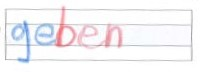
\includegraphics[]{figures/Schreibliniensystem.jpg}
    \caption{Schreibliniensystem mit Oberband (Bereich zwischen der oberen und der zweiten Linie von oben), Mittelband (zwischen den beiden mittleren Linien) und Unterband.}
    \label{Schreibliniensystem}
\end{figure}

\is{Ober- und Unterlängen}Ober- und Unterlängen sind die Teile eines Buchstaben, die über das sogenannte Mittelband hinausragen. Abbildung~\ref{Schreibliniensystem} zeigt die Schreibung \textit{geben} in einem Schreibliniensystem für Erstklässler. Der Bereich zwischen den beiden mittleren Linien ist das Mittelband. Das Feld darüber nennt man das Oberband, das darunter das Unterband. Oberlängen befinden sich im Oberband, Unterlängen im Unterband. <g> hat also eine Unterlänge, <b> eine Oberlänge \citep[192--193]{FuhrhopPeters2013}. 

Silbengrenzen erkennt man im Geschriebenen  an den Ober- und Unterlängen \citep[217--221]{FuhrhopPeters2013}. Die Buchstabenform übernimmt in der geschriebenen Sprache also die Funktion, die die Sonorität der Laute (vgl. Abschnitt~\ref{subsec:Sonoritaet}), in der gesprochenen Sprache hat. Phonologisch gesehen beginnt das Wort \textit{geben} wenig sonor mit einem Plosiv. Die geringe Sonorität wird durch die Unterlänge des Buchstaben \textit{g} angezeigt. Bis zum Vokal \textipa{[e:]} steigt die Sonorität an. In der Schrift kann man das daran erkennen, dass das \textit{e} keine Ober- oder Unterlänge hat. Dann sinkt die Sonorität wieder ab bis zum \textipa{[b]}. Die Silbengrenze liegt also vor dem \textit{b}, dem Buchstaben mit der Oberlänge. Die hohe Sonorität des nächsten Sonoritätsgipfels kann man in der Schrift daran erkennen, dass \textit{e} keine Ober- oder Unterlänge hat. \textipa{[n]} ist ein sonorer Konsonant, der Buchstabe \textit{n} hat deshalb ebenfalls keine Ober- oder Unterlänge.

Allgemein kann man sagen, dass wenig sonore Laute meist Buchstaben mit Ober- oder Unterlängen entsprechen: \textit{p, b, t, d, k, g, h}. Die hochsonoren Vokale entsprechen Buchstaben ohne Ober- und Unterlängen: \textit{a, e, i, o, u}. 

Ober- und Unterlängen haben, wie \citet{Drews2011} zeigt, einen messbaren Einfluss auf die Lesegeschwindigkeit und Lesegenauigkeit. Das liegt daran, dass geübte Leserinnen und Leser nicht Buchstabe für Buchstabe lesen, sondern größere Einheiten auf einmal erfassen (\zB \cite{Scheerer-Neumann1998}). Über die Bereiche, die sie nicht genau lesen, stellen die Leserinnen und Leser Hypothesen an. Dabei helfen ihnen die Ober- und Unterlängen. Wenn sie anhand dieser beispielsweise wissen, dass ein Wort drei Silben hat, können sie eine deutlich präzisere Voraussage machen, um welches Wort es sich handeln könnte als wenn sie keine Information über die Anzahl der Silben haben.

Der Zusammenhang zwischen geringer Sonorität und den Ober- oder Unterlängen ist nicht absolut. Eine Ausnahme ist \textit{s}, ein Buchstabe, der meistens an Silbengrenzen steht, aber keine Ober- oder Unterlänge hat. Interessant ist in diesem Zusammenhang jedoch die Entwicklung, die das Deutsche in den letzten Jahrhunderten erlebt hat. Für das stimmlose \textipa{[s]} hat sich das \textit{ß}, ein Buchstabe mit Oberlänge, entwickelt \citep[199--200]{FuhrhopPeters2013}. Das Schreibsystem hat sich also in gewisser Weise repariert.

Als zweites Beispiel für die Entwicklung zu einer besseren Markierung von Silbengrenzen hin wird das \textit{y} betrachtet. Als Buchstabe mit Unterlänge ist es nicht gut geeignet, um einen vokalischen Silbenkern zu repräsentieren. Während das \textit{y} im Frühneuhochdeutschen aber noch sehr häufig war, wird es seitdem immer weiter verdrängt und durch <i> ersetzt, einen Buchstaben, welcher ohne Ober- und Unterlänge ein besserer graphematischer Silbenkern ist \citep[220--221]{FuhrhopPeters2013}.



\section{Buchstaben und Grapheme}\label{sec:BuchstabenGrapheme}

\is{syllabische Schrift}\is{Alphabetschrift}\is{logographische Schrift} Im Allgemeinen werden nach \citet[69--70]{Duerscheid2016} drei Schrifttypen unterschieden: der \textit{logographische} Schrifttyp, der \textit{syllabische} Schrifttyp und der \textit{alphabetischen} Schrifttyp. Bei Schriftsystemen vom logographischen Schrifttyp, zu denen etwa das Chinesische gehört, entspricht ein Schriftzeichen in der Regel einer bedeutungstragenden Einheit (\zB einem Wort oder einem Morphem). Bei Schriftsystemem vom syllabischen und alphabetischen Typ hingegen entsprechen die Schriftzeichen \textit{bedeutungsunterscheidenden Einheiten} (Silben beim syllabischen Typ, \zB Japanisch, und Lauten beim alphabetischen Typ, \zB Deutsch, Russisch, Griechisch).

Wenn ein Schriftzeichen in einer Alphabetschrift bedeutungsunterscheidend ist, bezeichnet man es als \textit{Graphem} \citep[202]{FuhrhopPeters2013}.

\begin{Definition}{Grapheme}\label{def:Grapheme}
    
\noindent Grapheme sind die kleinsten bedeutungsunterscheidenden Einheiten der Schriftsprache.
\end{Definition}



Ähnlich wie die Phoneme (Definition~\ref{def:Phonem}), gewinnt man die Grapheme eines Schriftsystems durch \textit{Minimalpaaranalyse}\is{Minimalpaar}. Dafür stellt man zwei Wörter, die sich in einem einzigen Schriftzeichen unterscheiden, gegenüber. Haben die beiden Wörter auch unterschiedliche Bedeutung, sind die beiden unterschiedlichen Schriftzeichen Grapheme. Wenn man beispielsweise \textit{als} und \textit{alt} vergleicht, stellt man fest, dass sie sich in einem Schriftzeichen unterscheiden, \textit{s} vs. \textit{t}. Außerdem gibt es einen Bedeutungsunterschied. Daraus kann man schlussfolgern, dass <s> und <t> Grapheme sind. Grapheme setzt man in spitze Klammern. 

\is{Graphem}Grapheme können aus genau einem Buchstaben bestehen, dann bezeichnet man sie als \textit{einfache Grapheme}\is{Graphem!einfach}, \zB <s, t, a, w>. Es gibt aber auch Grapheme, die aus mehreren Buchstaben bestehen (\textit{komplexe Grapheme})\is{Graphem!komplex}. Man kann etwa \textit{mich} und \textit{mit} kontrastieren und dadurch zeigen, dass <ch> und <t> Grapheme sind. <ch> ist ein komplexes Graphem, so wie auch <qu> und <sch>. Ein vokalisches komplexes Graphem ist <ie>.


Es ist wichtig, Buchstaben und Grapheme nicht gleichzusetzen. Es gibt
\begin{itemize}
    \item Buchstaben, die Grapheme des Deutschen sind, \zB <e>,
    \item Buchstaben, die keine Grapheme des Deutschen sind, \zB \textit{q},
    \item mehrere Buchstaben, die zusammen ein Graphem bilden \zB <ch>.
\end{itemize}


Das\is{Grapheminventar} im Folgenden aufgelistete Grapheminventar des Deutschen orientiert sich an der \citet[909f]{Duden2022}. Hinzugefügt sind lediglich die Schreibdiph\-thonge. Hier orientieren wir uns an \citet[210, 222]{FuhrhopPeters2013}, die bei der Auflistung der Graphem-Phonem-Korrespondenzen zwar keine Korrespondenzen zwischen lautlichen Diphthongen und Schreibdiphthongen angeben, später aber genau diese Korrespondenzen diskutieren. Die Annahme von Schreibdiphthongen als Grapheme kann man mit Minimalpaaren wie \textit{fielen - feilen, freuen - Frauen} begründen. Diese Grapheme anzunehmen ist außerdem sinnvoll für didaktische Implikationen.


\ea
\textit{Grapheminventar des Deutschen}\\
    \begin{itemize}
        \item einfache Grapheme: \textit{a, b, d, e, f, g, h, i, j, k, l, m, n, o, p, r, s, t, u, v, w, x, z, ß, ä, ö, ü}
        \item komplexe Grapheme: \textit{ch, qu, sch, ng, ie, ei, au, eu}
    \end{itemize}
\z



Einige der hier angegebenen Grapheme sind umstritten. Gegen das Graphem <ng> wird argumentiert, dass es zwei Lauten entspricht, von denen einer durch einen phonologischen Prozess getilgt wird (vgl. Abschnitt~\ref{sec:gTilgung}). \citet[94--97]{Nerius1989} bezeichnet <ng> als \gqq{Buchstabenverbindung}. \citet[209]{FuhrhopPeters2013} listen <ng> nicht als Phonem, führen es in Klammern allerdings bei den Phonem-Graphem-Beziehungen auf.  

Außerdem stellen \citet[205]{FuhrhopPeters2013} den Graphemstatus von <sch> infrage. Mittels der Minimalpaare \textit{Masche -- manche -- Maske}  zeigen sie, dass <s> und <ch> separat ersetzbar sind. Das Minimalpaar \textit{Masche -- manche} zeigt demnach, dass das <s> innerhalb des <sch> ein Graphem ist. Das Minimalpaar \textit{Masche -- Maske} zeigt, dass das <ch> innerhalb des <sch> ein Graphem ist. Gegen diese Analyse kann man einwenden, dass ein Graphem eine lautliche Einheit repräsentiert. Wenn man <sch> als zwei Grapheme betrachtet, müsste diesen beiden Graphemen eine Phonemfolge entsprechen, was aber nicht der Fall ist.

Bei <ie> wird diskutiert, dass die Gespanntheit im Deutschen in der Regel nicht am Graphem selbst angezeigt wird (\cite[211]{FuhrhopPeters2013}, \cite[24]{Primus2010}). 

Die Buchstaben \textit{c, y} und \textit{q} sind keine Grapheme des Deutschen, denn es gibt keine Minimalpaare, wo etwa \textit{c} mit einem anderen Graphem kontrastiert. \textit{c} kommt allein (also nicht als <ch> oder <sch>) nur in Fremdwörtern vor. \textit{y} kommt überhaupt nur in Fremdwörtern vor. \textit{q} kommt nur in der Verbindung <qu> vor: \textit{Qual, Quelle, quaken}.\footnote{Es gibt Minimalpaare, bei denen <qu> als Ganzes ersetzt wird: \textit{Qual -- Wal}. Dieses Minimalpaar zeigt, dass <qu> und <w> Grapheme des Deutschen sind. Man kann auch das \textit{q} alleine ersetzen: \textit{Quelle -- Duelle}.  Es gibt aber keine Möglichkeit das \textit{u} von <qu> zu ersetzen (etwa \textit{Quelle -- *Qielle}), cf. \citet[204]{FuhrhopPeters2013}.}

Die eher sprachdidaktisch orientierte Forschung tendiert dazu, <ng>, <sch>, <ie> und die Schreibdiph\-thonge als Grapheme zu behandeln, etwa \citet[21--22]{SchruenderLenzen2013}, die sich auf \citet{Thome2000a} bezieht.


\section{Phonem-Graphem-Korrespondenzen}\label{sec:PGK}

In Alphabetschriften gibt es regelhafte Entsprechungen zwischen Phonemen und Graphemen. Diese Entsprechungen nennt man \textit{Phonem-Graphem-Korres\-pon\-den\-zen}. Beispielsweise entspricht dem  Phonem \textipa{/l/} das Graphem <l>: \textit{leicht, Wal, Fohlen}. Bei den meisten Graphemen sind die Entsprechungen aber nicht 1:1. Beispielsweise kann ein \textipa{/p/} als <p> (\textit{Paar}), als <pp> (\textit{Klippe}) oder als <b> (\textit{hinab}) geschrieben werden. \citet[95--97]{Nerius1989} stellt die Beziehungen zwischen Phonemen und Graphemen daher konsistent als 1:x-Beziehungen dar. Wie weiter unten ausgeführt, folgt die sprachdidaktische Literatur bis heute diesem Ansatz. In der linguistischen Literatur hingegen, \zB in der \citet[910]{Duden2022}, wird jedem Phonem ein einziges Graphem zugeordnet, \zB dem \textipa{/p/} das <p>. Anders geartete Schreibungen, also <pp> oder <b> werden durch die weiteren graphematischen Prinzipien erklärt.

In den Tabellen~\ref{tab:PGBKonsonanten} und \ref{tab:PGBVokale} sind die Korrespondenzen in Anlehnung and die \citet[910--911]{Duden2022} dargestellt. Die IPA-Symbole entsprechen dabei denen, die in Kapitel~\ref{kap:Phonologie} eingeführt wurden. Nicht in der Duden-Grammatik aufgeführt sind die Korrespondenzen zwischen der Phonemfolge \textipa{/kv/} und <qu> und zwischen \textipa{/\t{ts}/} und <z>, die wir aber aufnehmen, weil wir <qu> und <z> als Graphem annehmen. Die \citet[911]{Duden2022} listet außerdem eine Korrespondenz zwischen \textipa{/\ae/} und <ä> auf. Wir folgen hier der phonetischen Literatur, die für das Deutsche nicht den Laut \textipa{[\ae]}, sondern das \textipa{[E]} vorsieht.


Während es bei den Konsonanten eine 1:1-Beziehung gibt -- jedem Phonem entspricht ein Graphem und umgekehrt (Tabelle~\ref{tab:PGBKonsonanten}) -- ist das bei den Vokalen nicht der Fall. Meist werden zwei Phoneme, ein ungespannter und ein gespannter Vokal, durch ein Graphem repräsentiert. Es existiert also eine 2:1- bzw. für <e> sogar eine 3:1-Beziehung. 1:1-Beziehungen gibt es nur bei \textipa{/i/} -- <ie> und \textipa{/I/} -- <i> (Tabelle~\ref{tab:PGBVokale}).

\begin{table}
    \centering
        \caption{\label{tab:PGBKonsonanten} Phonem-Graphem-Beziehungen für die Konsonanten}
    \begin{tabular}{llll}\lsptoprule
         Phoneme & Grapheme & Phoneme & Grapheme\\\midrule
         \textipa{/p/}&<p> & \textipa{/x/}&<ch>\\
         \textipa{/t/}&<t> & \textipa{/v/}&<w>\\
         \textipa{/k/}&<k> & \textipa{/z/}&<s>\\
         \textipa{/kv/}&<qu> & \textipa{/j/}&<j>\\
         \textipa{/b/}&<b> & \textipa{/h/}&<h>\\
        \textipa{/d/}&<d> & \textipa{/m/}&<m>\\
         \textipa{/g/}&<g> & \textipa{/n/}&<n>\\
         \textipa{/f/}&<f> & \textipa{/N/}&<ng>\\ 
         \textipa{/s/}&<ß> & \textipa{/l/}&<l>\\
         \textipa{/S/}&<sch> & \textipa{/K/}&<r>\\ 
         \textipa{/\t{ts}/}&<z> &\\\lspbottomrule
    \end{tabular}
\end{table}



\begin{table}
    \centering
    \begin{tabular}{llllll}\lsptoprule
         \multicolumn{2}{c}{gespannte Vokale}& \multicolumn{2}{c}{ungespannte Vokale}& \multicolumn{2}{c}{Diphthonge}\\
         Phoneme & Grapheme & Phoneme & Grapheme& Phoneme & Grapheme\\\midrule
         \textipa{/i/}&<ie> & \textipa{/I/}&<i>& \textipa{/\t*{aU}/}& <au>\\
         \textipa{/y/}&<ü> & \textipa{/Y/}&<ü>& \textipa{/\t*{OI}/}&<eu>\\
        \textipa{/e/}&<e> &\textipa{/E/}&<e>&\textipa{/\t*{aI}/}& <ei>\\
         \textipa{/\o/}&<ö> &\textipa{/\oe/}&<ö>\\
         \textipa{/a/}&<a> & \textipa{/a/}&<a>\\
         \textipa{/o/}&<o>& \textipa{/O/}&<o>\\
         \textipa{/u/}&<u> & \textipa{/U/}&<u>\\
          \textipa{/E/}&<ä> &\textipa{/@/}&<e>&\\ 
\lspbottomrule
    \end{tabular}
    \caption{\label{tab:PGBVokale} Phonem-Graphem-Beziehungen für die Vokale}
\end{table}

In der sprachdidaktischen Literatur geht man von 1:x-Beziehungen aus. \citet[84--93]{Thome2019} beispielsweise unterscheidet zwischen  \textit{Basisgraphemen} und \textit{Orthographemen}. Ein Phonem entspricht einem Basisgraphem und eventuell einem oder mehreren Orthographemen. Die Tabellen~\ref{BasisgraphemeOrthographeme1}  und \ref{BasisgraphemeOrthographeme2}  sind aus \citet{Thome2019} übernommen.

\begin{table}
    \centering
    \footnotesize
    \begin{tabular}{llllll}\lsptoprule
         Pho-&Basisgrapheme& \multicolumn{4}{c}{Orthographeme}\\
         eme&meist oder immer & manchmal & gelegentlich & selten & sehr selten\\\midrule
         \textipa{/n/}&<n> Nase & --&--&<nn> Tanne&--\\\hline
         \textipa{/r/}&<r> Rad &- &--&--&<rr> wirr\\
         &&&&&<rh> Rhein\\\hline
        \textipa{/t/}&<t> Tisch &-&<d> Bild&<tt> Mitte&<dt> Stadt\\
        &&&&&<th> Thron\\\hline
         \textipa{/d/}&<d> Dach&--&--&--&<dd> Kladde\\\hline
         \textipa{/l/}&<l> Lampe &--&<ll> Ball&--&--\\\hline
         \textipa{/s/}&<s> Eis& &<ss> Kuss&<ß> Gruß&-\\\hline
         \textipa{/x/}&<ch> Bach&--&--&<g> König&\\\hline
         \textipa{/m/}&<m> Maus&-- &<mm> Kamm&--&--\\\hline
         \textipa{/z/}&<s> Seil& --&--&--&--\\\hline
         \textipa{/f/}&<f> Fisch&<v> Vogel &--&<ff> Schiff&<ph> Physik\\\hline
         \textipa{/v/}&<w> Wiese& --&--&--&<v> Vase\\\hline
         \textipa{/g/}&<g> Gabel& --&--&--&<gg> Egge\\\hline
         \textipa{/k/}&<k> Kuchen&<g> Berg &<ck> Ecke&-&<ch> Chor\\
         &&&&&<c> Clown\\\hline
         \textipa{/b/}&<b> Buch& --&--&--&<bb> Ebbe\\\hline
         \textipa{/S/}&<sch> Schaf& <s> Spiel&-&-&-\\\hline
         \textipa{/h/}&<h> Haus& --&--&-&--\\\hline
         \textipa{/\t{ts}/}&<z> Zaun& -&<tz> Katze&--&--\\\hline
         \textipa{/p/}&<p> Pinsel& <b> Laub&--&<pp> Treppe&--\\\hline
         \textipa{/N/}&<ng> Ring& --&<n> Bank&--&--\\\hline
         \textipa{/j/}&<j> Junge& --&--&--&--\\\hline
         \textipa{/\t{pf}/}&<pf> Pferde Seil& --&--&--&--\\\hline
         \textipa{/\t{ks}/}&<chs> Fuchs& <x> Hexe&--&--&--\\
\lspbottomrule
    \end{tabular}
    \caption{\label{BasisgraphemeOrthographeme1}Basis- und Orthographeme der Konsonanten, übernommen aus: \citet[89]{Thome2019}}
\end{table}


\begin{table}
    \centering
    \footnotesize
    \begin{tabular}{llllll}\lsptoprule
         Pho-&Basisgrapheme& \multicolumn{4}{c}{Orthographeme}\\
         neme&meist oder immer & manchmal & gelegentlich & selten & sehr selten\\\midrule
         \textipa{/@/} & <e> Hase&-- &-- &-- &--\\\hline
         \textipa{/I/} & <i> Insel&-- &-- &-- &<ie> vierzig\\\hline
         \textipa{/a/} & <a> Apfel&-- &-- &-- &--\\\hline
         \textipa{/i:/} & <ie> Biene&-- &<ih> ihr &<i> Igel &<ieh> sieht\\\hline
         \textipa{/e:/} & <e> Feder&-- &<eh> sehr &-- &<ee> See\\\hline
         \textipa{/a:/} &<a> Glas &-- &-- &<ah> sah &<aa> Haar\\\hline
         \textipa{/E/} & <e> Zelt&-- &<ä> hält &-- &--\\\hline
         \textipa{/\t*{aI}/} & <ei> Ei &-- &-- &-- &<eih> Geweih\\
         &&&&&<ai> Mais\\\hline
         \textipa{/U/} & <u> Muschel&-- &-- &-- &--\\\hline
         \textipa{/O/} & <o> Frosch&-- &-- &-- &--\\\hline
         \textipa{/o:/} & <o> Hose&-- &<oh> Sohn &-- &<oo> Boot\\\hline
         \textipa{/u:/} & <u> Blume&-- &-- &<uh> Kuh &--\\\hline
         \textipa{/\t*{aU}/} & <au> Auto &-- &-- &-- &--\\\hline
         \textipa{/y:/} &  <ü> Hüte&<üh> Kühe &-- &-- &--\\\hline
         \textipa{/Y/} & <ü> Büsche&-- &-- &-- &--\\\hline
         \textipa{/\o:/} &<ö> Löwe &-- &<öh> Söhne &-- &--\\\hline
         \textipa{/\t*{OY}/} & <eu> Eule&&<äu> läuten  &-- &--\\\hline
         \textipa{/E:/} &<ä> Käse &<äh> Fähre &-- &-- &--\\\hline
         \textipa{/\oe /} &<ö> Töpfe &-- &-- &-- &--\\
         \lspbottomrule
    \end{tabular}
    \caption{\label{BasisgraphemeOrthographeme2}Basis- und Orthographeme der Vokale, übernommen aus: \citet[89]{Thome2019}}
\end{table}
         

\is{Basisgraphem}Basisgrapheme sind Grapheme, die häufig vorkommen. \is{Orthographem}Orthographeme sind Grapheme, die selten vorkommen. Thomé geht davon aus, dass der Erwerb der Basisgrapheme dem der Orthographeme vorangeht. Zum Beispiel wird <p> als Basisgraphem für das Phonem \textipa{/p/} zuerst erworben; <b> oder <pp> sind Orthographeme für \textipa{/p/} und werden daher später erworben \citep[89--90]{Thome2019}. 

Die Korrespondenzen bei den s-Lauten unterscheiden sich ebenfalls. Während die \citet[910]{Duden2022} von einer 1:1-Zuordnung ausgeht: \textipa{/s/} -- <ß> und \textipa{/z/} -- <s>, nimmt \citet{Thome2019} <s> als Basisgraphem für beide Laute, \textipa{/s/} und \textipa{/z/} an, weil der Laut \textipa{[s]} durch die Auslautverhärtung häufig <s> geschrieben wird.

Genau wie die Duden-Grammatik geht Thomé bei den Vokalgraphemen von einer grundsätzlichen 2:1-Beziehung zwischen Phonemen und Basisgraphemen aus. So entspricht dem Basisgraphem <u> das Phonem \textipa{/u:/} (\textit{Blume}), aber auch das Phonem \textipa{/U/} (\textit{Muschel}). Bei <e> gibt es -- wie in der \citet{Duden2022} -- eine 1:3-Beziehung. Diesem Graphem entsprechen die Phoneme \textipa{/@, e, E/}, etwa in den Wörtern \textit{Hase, Feder, Zelt}. Bei den i-Lauten nimmt Thomé -- wie die Duden-Grammatik -- eine 1:1-Beziehung an: <ie> entspricht \textipa{/i:/} und <i> entspricht \textipa{/I/}.\footnote{Die Unterscheidung zwischen Basisgraphemen und Orthographemen ist insofern nützlich, als man im Erwerb tatsächlich beobachten kann, dass zunächst die Basisgrapheme und erst danach die Orthographeme erworben werden. Strenggenommen sind jedoch die Orthographeme häufig keine Grapheme, denn Grapheme sind die \textit{kleinsten} bedeutungsunterscheidenden Einheiten der Schriftsprache. \citet[89]{Thome2019} listet beispielsweise für \textipa{/a:/} als Basisgraphem <a> wie in \textit{Glas} und als Orthographem <ah> wie in \textit{sah} auf. Da man sowohl das <h> als auch das <a> ersetzen kann, um ein Minimalpaar zu bilden (\textit{Sau} und \textit{sieh}), handelt es sich bei <ah> nicht um die kleinste bedeutungsunterscheidende Einheit. Diesen Einwand kann man -- wie bei \citet{FuhrhopThierrof2005} dargestellt -- zwar auch beim <sch> bringen. Bei <sch> kann man jedoch argumentieren, dass <s> und <ch> anderen Lauten entsprechen als <sch>. Ein weiterer Einwand gegen den Phonembegriff bei Thomé ist, dass <chs> zwar eine häufige Schreibung ist, das ihm zugeordnete \textipa{/ks/} jedoch kein Phonem, sondern eine Phonemfolge ist. Deshalb sind viele Autor(inn)en der Meinung, dass <chs> eigentlich zwei Grapheme sind, <ch> und <s>, \zB \citet[96]{Nerius1989}, der bei \textit{Wachs} eine Entsprechung <ch> -- \textipa{/k/} und eine weitere <s> -- \textipa{/s/} annimmt.}

\largerpage
Ein Vorteil von Thomés Ansatz ist, dass er Erwerbsreihenfolgen gut erklärt. Beispielsweise wird \textipa{/s/} durch die Auslautverhärtung tatsächlich häufig <s> geschrieben und diese Zuordnung wird auch früher erworben als die \textipa{/s/} -- <ß>-Zuordnung.

\largerpage
Ein Nachteil des Ansatzes von Thomé ist, dass die Annahme von Orthographemen wenig erklärt und damit die Chance vertan wird, Regelhaftes in der Orthografie als solches zu erkennen. Auch das kann man an der Analyse der s-Laute zeigen. Thomé erklärt mit der Zuordnung von \textipa{/s/} und \textipa{/z/} zu <s> nur, dass die meisten Wörter, in denen \textipa{[s]} gesprochen wird, mit <s> geschrieben werden. Das stimmt, es hilft aber nicht, wenn man sich fragt, ob man \textit{Gras} oder \textit{*Graß} schreiben muss. Hier wird Regelhaftes als arbiträr dargestellt: Bei \textit{Gras} und \textit{Eis} handelt es sich um Schreibungen, die morphologisch (also über Ableitungen) zu begründen sind. Man schreibt \textit{Gras}, weil es \textit{Gräser} (mit \textipa{[z]}) gibt und \textit{Eis}, weil es \textit{eisig} (mit \textipa{[z]}) gibt.

\newpage
Auch die Schreibung der Doppelkonsonanz wird als etwas Arbiträres dargestellt. Nach Thomés Ansatz müsste man die Schreibung \textit{Mitte} mit zwei unabhängigen Überlegungen begründen: (1) <i> ist das Basisgraphem von \textipa{/I/}, (2) <tt> ist ein Orthographem von \textipa{/t/}. Dass beides miteinander zusammenhängt, dass man die Aussprache \textipa{/I/} also aus der Schreibung <tt> ableiten kann, wird durch diese Analyse nicht klar.

Linguistisch gesehen ist es also wenig sinnvoll, Orthographeme überhaupt als Grapheme anzusehen. Davon abgesehen werden durch sie regelhafte Schreibungen als arbiträr dargestellt. Deshalb werden wir im Folgenden als Phonem-Graphem-Korrespondenzen die Korrespondenzen aus der \citet[]{Duden2022} betrachten, die meist den Korrespondenzen zwischen Phonemen und Basisgraphemen bei Thomé entsprechen. Die Schreibungen, die Thomé als Orthographeme bezeichnet, werden wir über die weiteren Prinzipien der Orthografie erklären.

\section{Graphematische Prinzipien}\label{sec:GraphPrin}\is{graphematische Prinzipien}
Die Schreibung des Deutschen ist durch bestimmte Grundsätze geprägt. Diese Grundsätze nennt man \textit{graphematische Prinzipien}. Der wichtigste Grundsatz jeder Alphabetschrift ist das \textit{phonographische Prinzip}. Nach diesem Prinzip wird jedem Phonem ein Graphem zugeordnet. Nach dem \textit{silbischen Prinzip} kennzeichnet man bei Schreibungen Eigenschaften, die mit der Silbenstruktur zu tun haben, beispielsweise ein Silbengelenk durch eine Doppelkonsonanz (\zB \textit{Fussel}). Nach dem \textit{morphologischen Prinzip} schreibt man verwandte Stämme gleich oder zumindest ähnlich (\zB \textit{Stämme} mit <ä>, weil der Singular \textit{Stamm} ist). Nach dem \textit{syntaktischen Prinzip} schreibt man so, dass man die syntaktische Struktur einer Äußerung erkennen kann. Die Großschreibung nominaler Köpfe (Substantive) ist eine Ausprägung des syntaktischen Prinzips. Einige Schreibungen lassen sich darüber erklären, dass man versucht, gleichlautende Wörter (etwa \textit{Leib -- Laib}) unterschiedlich zu schreiben. Diese Schreibungen lassen sich über das \textit{Homographievermeidungsprinzip} erklären. In der Literatur werden noch weitere Prinzipien diskutiert, etwa das ästhetische Prinzip oder das historische \citep[88--98]{Nerius2007} die wir hier aussparen wollen.

Die Reihenfolge, in welcher die Prinzipien diskutiert werden, ist nicht willkürlich. Das zuerst genannte Prinzip, das phonographische, ist zugleich das dominanteste. Das zuletzt genannte Homographievermeidungsprinzip hat deutlich weniger Einfluss. Wenn Prinzipien miteinander konkurrieren, \gqq{gewinnt} in der Regel das grundlegendere Prinzip. Die Erwerbsreihenfolge der ersten vier Prinzipien entspricht in etwa der hier angegebenen Reihenfolge, d.\,h. zunächst schreiben Lernende nach dem phonographischen Prinzip, später kommen silbische Schreibungen dazu, noch später morphologische. Schreibungen nach dem syntaktischen Prinzip werden manchmal erst gegen Ende der Schulzeit perfektioniert (vgl. Abschnitt~\ref{sec:Erwerbsreihenfolgen}). 


\subsection{Phonographisches Prinzip}
\label{Absatz_phon_prin}


Das \textit{phonographische Prinzip} (auch \textit{phonologisches} oder \textit{phonematisches Prinzip, Lautprinzip}) lässt sich vereinfacht wie folgt fassen:


\begin{Definition}{Phonographisches Prinzip}\\
\noindent Den lautlichen Elementen (Phonemen) sind in der Schriftsprache schriftliche Elemente (Grapheme) zugeordnet.\footnote{Für explizitere Formulierungen cf. etwa \citet[144]{Duerscheid2016}, \citet[40]{GallmannSitta1996}.}
\end{Definition}

Im Folgenden werden vier Wörter betrachtet: \textit{mit, mich, bitte} und \textit{Kiel}. Das Wort \textit{mit} besteht im Standard aus drei Phonemen: \textipa{/mIt/}. Um die \textit{phonographische Schreibung} zu ermitteln, wird jedes Phonem durch das Graphem ersetzt, welches ihm laut Graphem-Phonem-Korrespondenzen entspricht (Tabellen~\ref{tab:PGBKonsonanten},  Seite \pageref{tab:PGBKonsonanten}, und \ref{tab:PGBVokale}, Seite \pageref{tab:PGBVokale}): 

\ea
\begin{tabular}{lccc}
Phoneme: & \textipa{/m/} & \textipa{/I/} & \textipa{/t/}\\
&| & | & |\\
Grapheme: & <m> & <i> & <t>\\
\end{tabular}
\z

Die Schreibung <mit> wird als phonographische Schreibung bezeichnet, denn sie ergibt sich allein aufgrund der Graphem-Phonem-Korrespondenzen.

Das Wort \textit{mich} besteht ebenfalls aus drei Phonemen: \textipa{/mIç/}. Nun wird wieder jedes der Phoneme durch das entsprechende Graphem ersetzt: \textipa{/m/} durch <m>, \textipa{/I/} durch <i> und \textipa{/ç/} durch das komplexe Graphem <ch>:

\ea \begin{tabular}{lccc}
Phoneme: & \textipa{/m/} & \textipa{/I/} & \textipa{/ç/}\\
&| & | & |\\
Grapheme: & <m> & <i> & <ch>\\
\end{tabular}
\z


Es ergibt sich die Schreibung <mich>. Auch diese Schreibung ist also phonographisch.

Das Wort \textit{bitte} besteht aus vier Phonemen: \textipa{/\textprimstress bI\.*{t}@/}. Man ersetzt wieder jedes dieser Phoneme durch ein Graphem:

\ea
\begin{tabular}{lcccc}
Phoneme: & \textipa{/b/} & \textipa{/I/} & \textipa{/t/} & \textipa{/@/}\\
&| & | & |&\\
Grapheme: & <b> & <i> & <t> & <e>\\
\end{tabular}
\z

Bei der Schreibung <bite> handelt es sich um eine \textit{phonographische} Schreibung, aber nicht um eine \textit{orthografische} Schreibung. Um zur orthografischen Schreibung zu gelangen, muss man weitere Prinzipien (in diesem Fall das silbische Prinzip) berücksichtigen.

\textit{Kiel} besteht aus drei Phonemen: \textipa{/ki:l/}. 

\ea
\begin{tabular}{lccc}
Phoneme: & \textipa{/k/} & \textipa{/i:/} & \textipa{/l/}\\
&| & | & \\
Grapheme: & <k> & <ie> & <l>\\
\end{tabular}
\z

Wenn man von der Großschreibung absieht, ist \textit{Kiel} also eine phonographische Schreibung, denn dem gespannten \textipa{/i/} entspricht als Graphem <ie>.

Schreibungen von Kindern zu Beginn des Schriftspracherwerbs orientieren sich zunächst vor allem am phonographischen Prinzip. Der folgende Text wurde von einer Zweitklässlerin geschrieben (Alter: 7;11). 

\ea
\ea
    \textit{Nach ein pa Wochen bekam die Muter en Kind das nanten sie Wiki. Wiki wuks her ran und waso gros widianderin. alz er 9 Jare alt wa sagte die Muter past auf die Hae auf. wensie euch Fresen dan seit ir Tot...}
\ex
    In Standardorthografie: \textit{Nach ein paar Wochen bekam die Mutter ein Kind, das nannten sie Wiki. Wiki wuchs heran und war so groß wie die anderen. Als er 9 Jahre alt war, sagte die Mutter: Passt auf die Haie auf. Wenn sie euch fressen, dann seid ihr tot...}
\z
\z

Der Text enthält Wörter, deren Orthografie sich tatsächlich nur aus dem phonographischen Prinzip ableitet: \textit{nach, Wochen, bekam, die, das} usw. Darüber hinaus schreibt das Kind Wörter phonographisch, bei denen für die orthografische Schreibung weitere Prinzipien beachtet werden müssen: Bei \textit{Jare, Fresen} das silbische Prinzip und bei den meisten Wörtern mit \textipa{/K/}-Vokalisierung (\textit{pa, wa}) das morphologische Prinzip.

Wenn man von der Groß- und Kleinschreibung, die hier noch sehr willkürlich eingesetzt wird, absieht, dann gibt es in diesem Text lediglich drei Schreibungen, bei denen andere Prinzipien als das phonographische Prinzip beachtet wurden: \textit{Kind} (statt phonographisch \textit{kint}), \textit{und} (statt phonographisch \textit{unt}) und \textit{sagte} (statt phonographisch \textit{sakte}). Da es sich um häufige Wörter handelt, ist es möglich, dass das Kind die anderen Prinzipien nicht im eigentlichen Sinne \gqq{beachtet} hat, sondern die Wörter memoriert hat.

Wenn man von \textit{Phonem-Graphem-Beziehungen} spricht, könnte man auch die \textipa{/g/}-Schreibung bei \textit{Tag} oder \textit{lustig} als Schreibung nach den Graphem-Phonem-Korrespondenzen annehmen, weil Phoneme nämlich -- im Unterschied zu den Phonen -- Abstraktionen über die (tatsächlich produzierten) Phone sind. Phoneme sind also die Einheiten, die im mentalen Lexikon repräsentiert sind. Die phonologische Repräsentation von \textit{Tag} ist \textipa{/ta:g/}, die von \textit{lustig} ist \textipa{/\textprimstress lUs.tIg/}. Demzufolge wären \textit{Tag} und \textit{lustig} phonographische Schreibungen. Da man Phänomene des Schriftspracherwerbs auf diese Weise aber nicht erklären kann, weil der Zugriff auf die phonologische Repräsentation erst erlernt werden muss, werden wir der \citet[913f]{Duden2022} folgen und solche Schreibungen als morphologische Schreibungen analysieren.



\begin{Exkurs}{\gqq{Lesen durch Schreiben}, Anlauttabellen und Igel-Syndrom}
\label{ExkursIgelsyndrom}

\noindent In vielen Schulen wird der Erwerb der Phonem-Graphem-Korrespondenzen durch die Arbeit mit einer \textit{Anlauttabelle}\is{Anlauttabelle} gestützt. In einer solchen Tabelle ist jedem Graphem das Bild eines Gegenstandes oder Lebewesens zugeordnet, dessen Bezeichnung mit dem Laut beginnt, der durch das Graphem repräsentiert wird. Neben dem <k> ist etwa ein Koffer, neben dem <b> eine Banane. Die extremste Form der Arbeit mit der Anlauttabelle ist wohl der -- besonders in den Medien sehr umstrittene -- Ansatz nach Reichen \textit{Lesen durch Schreiben}\is{Lesen durch Schreiben} (\cite[]{Reichen2008} und \cite{WiemerHuettenberger2015}). Reichen zufolge sollte das Schreiben mit der Anlauttabelle dem Lesen vorangehen. Die Kinder sollen also zunächst versuchen, Wörter mittels der Tabelle zu verschriften. Das Lesen lernen sie, indem sie die von ihnen selbst verschrifteten Wörter versuchen zu lesen.

Die Anlauttabelle hat eine Art Siegeszug durch die Fibellandschaft absolviert. Kaum ein Lehrwerk für die Schuleingangsphase kommt heute mehr ohne Anlauttabelle aus, selbst wenn die Lehrwerke sonst methodisch relativ fern von Reichen verortet werden können.

\begin{figure}[!htbp]
\centering
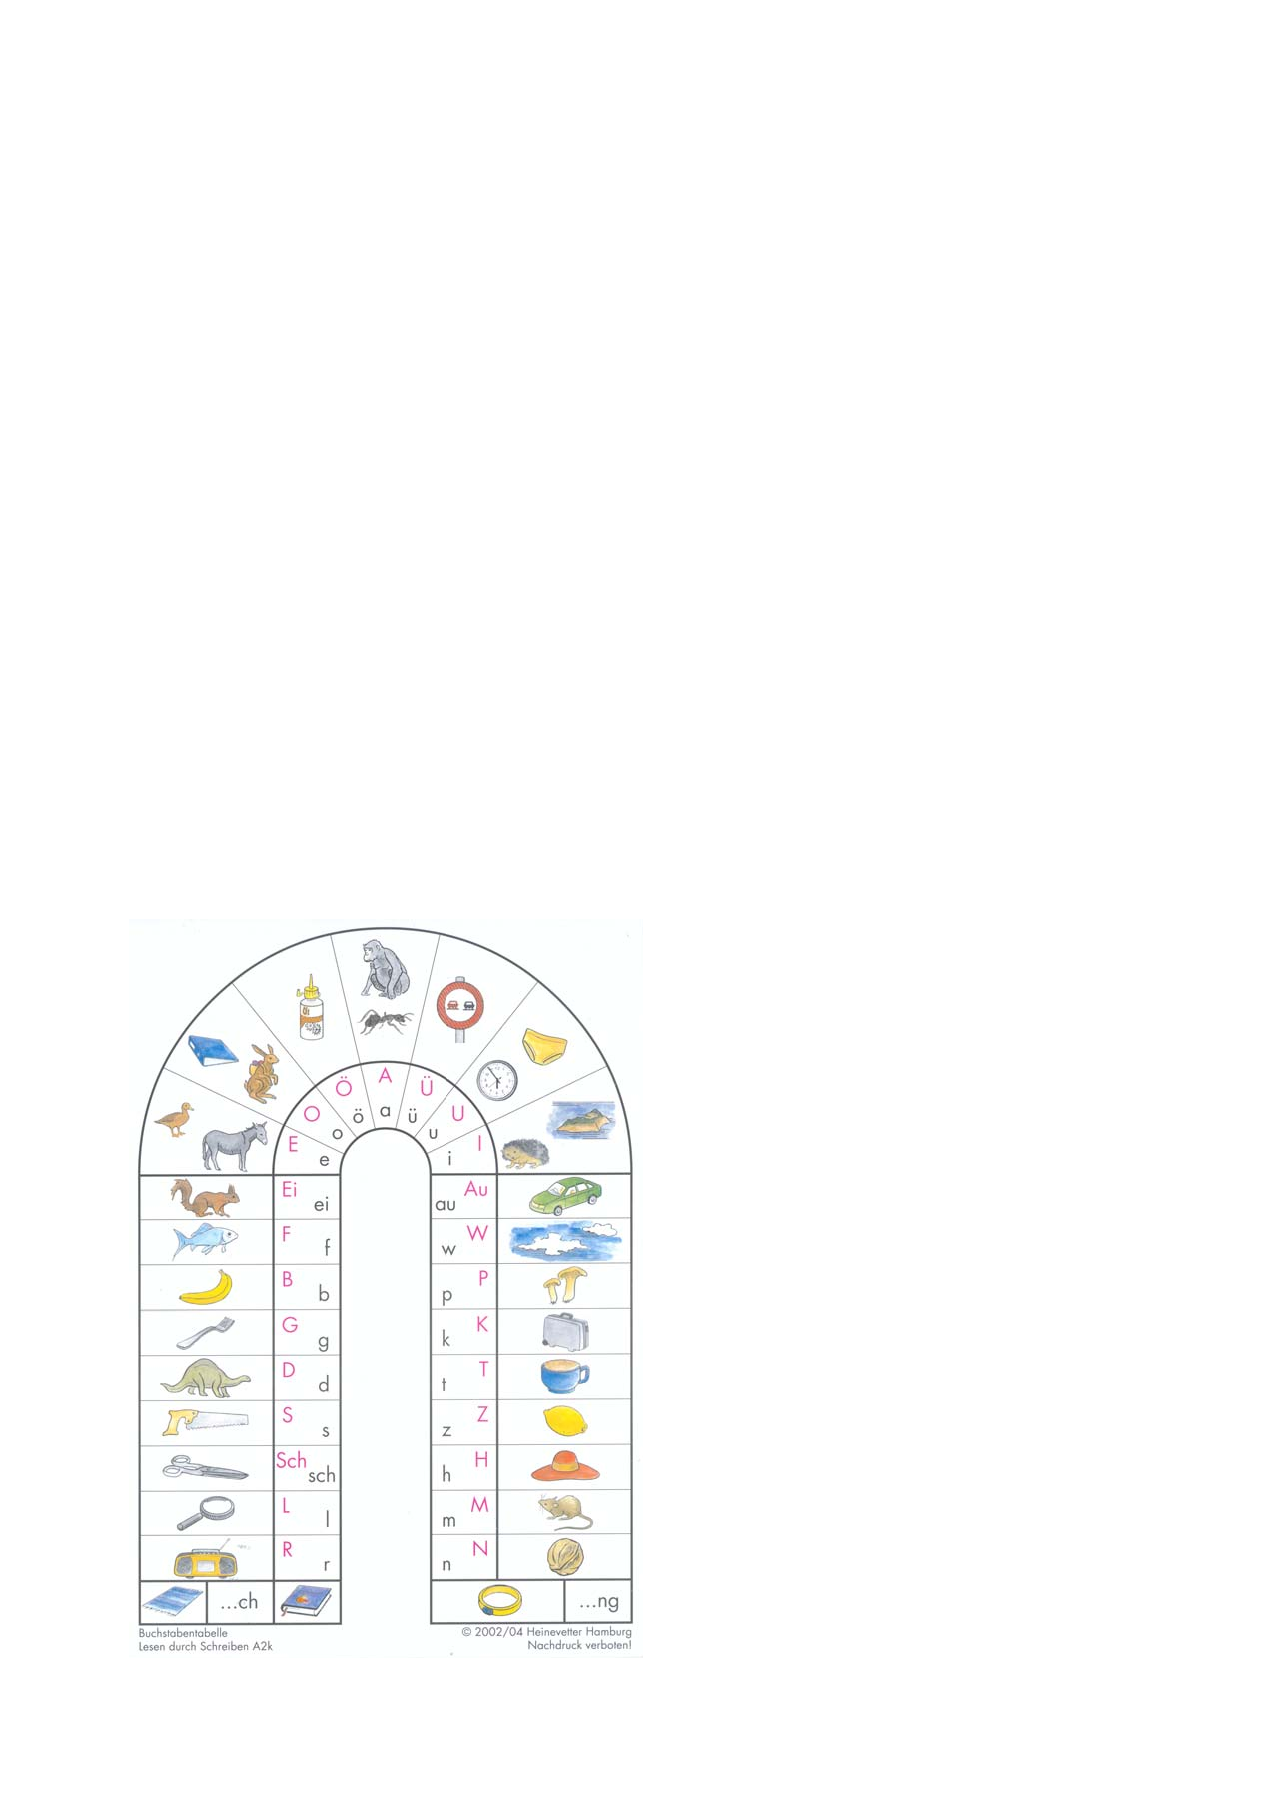
\includegraphics[width=.5\textwidth]{figures/Anlauttabelle_Reichen_2008.pdf}
\caption{Anlauttabelle aus \citet[4]{Reichen2008}}
\label{Anlauttabelle}
\end{figure}

Abbildung~\ref{Anlauttabelle} zeigt die Tabelle nach Reichen. Sie ist wie ein Tor geformt. In den Säulen stehen jeweils zwei Felder nebeneinander, im Bogen stehen sie übereinander. In dem einen der beiden Felder sind ein oder zwei Abbildungen zu sehen, in dem anderen ein Graphem (Großbuchstabe und Kleinbuchstabe). Die abgebildeten Lebewesen oder Gegenstände beginnen mit dem Laut, der über die Phonem-Graphem-Korrespondenzen dem jeweiligen Graphem zugeordnet ist. Der \textit{Dinosaurier} etwa beginnt mit dem Laut \textipa{/d/} und ist dem Graphem <D, d> zugeordnet. Die Konsonantengrapheme findet man in den beiden Säulen, die Vokalgrapheme im Bogen. Während man bei den Konsonantengraphemen eine 1:1-Relation findet (ein Bild pro Graphem), gibt es bei den Vokalgraphemen (außer bei <ü> und <ö>) zwei Bilder, die nur einem Graphem zugeordnet werden (\zB den \textit{Esel} für das gespannte \textipa{/e/} und die \textit{Ente} für das ungespannte \textipa{/E/}). 

Anlauttabellen sind im Prinzip Listen von Phonem-Graphem-Korres\-pon\-denzen für kindliche Nutzer. Reichen selbst hat unterschiedliche Anlauttabellen vorgeschlagen, \zB eine Erweiterung mit <eu, st, c, v, ä, pf, j, sp, x>. Die Tabellen der Schulbuchverlage heute unterscheiden sich zum Teil erheblich, vor allem in der Auswahl der bildlich dargestellten Beispielwörter. Für \textipa{/o/} beispielsweise wird \textit{Oma, Osterei} oder \textit{Ofen} angegeben, für \textipa{/l/} gibt es den \textit{Löwen} oder die \textit{Lupe}. Was jedoch immer gleich ist, ist die Korrespondenz zwischen \textipa{/i/} und dem \textit{Igel}. Wir werden gleich noch diskutieren, warum das so ist.

Warum ist die Methode nach Reichen so umstritten? Reichen selbst hat seine Methode nie wissenschaftlich evaluiert. Er beruft sich lediglich auf seine persönlichen Erfahrungen. Er argumentiert, dass die offene Unterrichtsform, die grundlegend für \textit{Lesen durch Schreiben} ist, die Motivation der Kinder hochhält, was sich positiv auf den Schriftspracherwerb auswirkt.

\citet{Weinhold2006} vergleicht in einer Longitudinalstudie den Schriftspracherwerb mittels der Reichen-Methode mit der silbenanalytischen Methode nach Röber (vgl. Exkurs~\ref{Exkurs:SAM}) und einem Fibellehrgang. Die Studie zeigt, dass die Reichen-Methode zumindest im ersten halben Schriftspracherwerbsjahr zu den besten Resultaten führt (S. 143). Die Anlauttabelle scheint für die Kinder in dieser Phase, wo sie sich vor allem am phonographischen Prinzip orientieren, also sehr nützlich zu sein. Danach überflügeln Klassen, die nach den anderen Methoden unterrichtet wurden, die Kinder, die nach der Reichen-Methode gelernt haben.

\citet{SchruenderLenzen2006} kann diesen anfänglichen Vorteil der Reichen-Methode in einer breit angelegten Studie nicht bestätigen. Die Kinder aus Klassen mit Fibellehrgängen erreichen am Ende der ersten Klasse bessere Werte (S. 34) im Rechtschreiben. Auch in der 3. Klasse sind die Fibelklassen den Klassen, die nach Reichen unterrichtet werden, überlegen (S. 35).

Neben der nicht nachgewiesenen Wirksamkeit\footnote{Nicht nachgewiesene Wirksamkeit ist ein Merkmal, welches diese Methode mit anderen teilt, cf. etwa \citet{BruegelmannBrinkmann2012}.} ist ein zweiter Grund dafür, dass die Methode umstritten ist, das sogenannte \textit{Igel-Syndrom}, cf. \citet[71]{Thome2019}\is{Igel-Syndrom}. Damit wird das Phänomen benannt, dass Kinder bis in die Mittelstufe hinein das gespannte \textipa{/i/} als <i> verschriften: <*Libe Oma!>; obwohl nach den Graphem-Phonem-Korrespondenzen <ie> geschrieben werden müsste. Bei <liebe> handelt es sich um eine phonographische Schreibung, also eine Schreibung nach dem phonographischen Prinzip. Obwohl phonographische Schreibungen generell früh erworben werden, sind ie-Fehlschreibungen häufig. \citet{Thome2000} argumentiert, dass das Igel-Syndrom eine direkte Folge der Arbeit mit der Anlauttabelle ist. In dieser Tabelle sind die Phonem-Graphem-Korrespondenzen für \textipa{/i, I/} schlicht falsch wiedergegeben. Für das ungespannte \textipa{/I/}, repräsentiert durch das Wort \textit{Insel}, wird richtigerweise <i> als Schreibung angegeben. Für das gespannte \textipa{/i/} wird mit <i> und dem \textit{Igel} jedoch eine falsche Korrespondenz angegeben.

Wenn die \textipa{/i/} -- <i>-Korrespondenz so selten vorkommt, warum verzichtet man dann nicht auf den \textit{Igel} und ersetzt ihn durch ein Wort mit der weitaus häufigeren Korrespondenz \textipa{/i/} -- <ie>? Das liegt daran, dass <ie> inital im Deutschen nicht vorkommt. Wörter, die mit \textipa{/i/} beginnen, werden mit <i> geschrieben: \textit{Igel, Iglu}. 

\citet[117]{Thome2000} schlägt deshalb statt einer Anlauttabelle eine Lauttabelle vor. Bei dieser Tabelle wird das Phonem \textipa{/i/} durch die \textit{Biene} repräsentiert. Damit wird die -- in der überwiegenden Mehrheit beobachtbare -- Graphem-Phonem-Korrespondenz \textipa{/i/} -- <ie> vermittelt. Es gibt inzwischen einige Lehrwerke, die das Problem angehen. Die Anlauttabelle der Tinto-Fibel etwa verzichtet zwar nicht auf den Igel, vermerkt aber zumindest die Möglichkeit der <ie>-Schreibung durch das Wort \textit{Knie} \citep[114]{Tintofibel}.
\end{Exkurs}

Zusammenfassend kann man feststellen, dass das phonographische Prinzip die Grundlage jeder Alphabetschrift ist. Jedem Phonem wird ein Graphem zugeordnet. Phonographische Schreibungen entstehen einzig und allein anhand dieser Zuordnung. Im Deutschen gibt es Wörter, die rein phonographisch geschrieben werden. Bei den meisten Schreibungen muss man jedoch weitere Prinzipien beachten.

\subsection{Silbisches Prinzip}\label{sec:silbischesPrinzip}
\is{silbisches Prinzip}

Die Beispiele im letzten Absatz haben gezeigt, dass phonographische Schreibungen nicht immer orthografisch sind. In den meisten Fällen greifen selbst bei der Schreibung einfacher Wörter mehrere Prinzipien. Viele betreffen die Silbe. Das liegt daran, dass -- wie eingangs erwähnt -- die Silbe für das Auge beim Lesen gut als Einheit erkennbar sein soll. Deshalb enthalten Schreibungen laut \citet[911ff]{Duden2022} auch silbenbezogene Informationen. 


Das silbische Prinzip hat vor allem zwei Ausprägungen: die \textit{Silbengelenksschreibung} (Konsonantenverdopplung oder \gqq{Schärfungsschreibung}\footnote{Der Begriff ist darauf zurückzuführen, dass die kurzen, ungespannten Vokale von einigen Sprecherinnen und Sprechern als scharf klingend empfunden werden.}) und die \textit{Dehnungsschreibung} (Doppelvokal oder \gqq{stummes h}).


\begin{Definition}{Silbisches Prinzip}

\noindent Schreibungen enthalten silbenbezogene Informationen, nämlich Informationen über die Vokallänge und das Vorhandensein eines Silbengelenks.


\end{Definition}



\subsubsection{Silbengelenksschreibungen}\label{sec:Silbengelenksschreibungen}
\is{Silbengelenksschreibung}


\subsubsubsection{Konsonantenverdopplung beim Silbengelenk}\is{Konsonantenverdopplung}
In Absatz~\ref{Absatz_phon_prin} wurde gezeigt, dass die Schreibung \textit{bitte} nicht allein über das phonographische Prinzip erklärt werden kann. Die phonographische Schreibung dieses Wortes ist <bite>. In der orthografischen Schreibung muss der Konsonant <t> verdoppelt werden.

In der didaktischen Literatur wird die Konsonantenverdopplung häufig \textit{Schärfungsschreibung}\is{Schärfungsschreibung} genannt. Zahlreiche erwachsene Schreiber(innen) formulieren die Regel für die Konsonantenverdopplung ähnlich wie in der folgenden Internetquelle\footnote{Richrath, Ulrike. 2020. Doppelkonsonanten: Zwei Regeln, die du dir leicht merken kannst. \url{https://die-lernlotsen.com/doppelkonsonanten-regeln} (28 Februar,
2020)}:

\begin{quote}
Hörst du den ersten Vokal im Wort kurz, dann schreibst du den nachfolgenden Mitlaut/ Konsonant [sic!] doppelt.[...] Hörst du den ersten Vokal im Wort lang, dann schreibst du den nachfolgenden Mitlaut nur einmal.
\end{quote}

Das stimmt für eine gewisse Anzahl an Wörtern: \textit{alle, Ratte, Fässer, Fälle, Hummel, Wippe, Fass, Fall} usw. Wenn man sich tatsächlich an diese Regel halten würde, würde man jedoch auch schreiben: \textit{*Felld, Hemmd, Hefft, Rosst, fünnf} usw. Die Regel scheint also falsch zu sein. Dass die Konsonantenverdopplung keine Folge der Aussprache des Vokals sein kann, zeigt auch der Vergleich zwischen Wörtern wie \textit{Sonne} und \textit{Sonde}. Die Vokale sind hier identisch und trotzdem wird der nachfolgende Konsonant einmal verdoppelt und das andere mal nicht. 

Andere Schreiberinnen und Schreiber des Deutschen geben an, sie würden die Doppelkonsonanten zweimal sprechen. Zu dieser Ansicht gelangen einige Sprecherinnen und Sprecher durch das Silbenklatschen von Wörtern mit Silbengelenk, bei denen der ambisilbische Konsonant doppelt gesprochen wird: \textit{al-le, Rat-te}. Auch zahlreiche Lehrmaterialien suggerieren, dass man ambisilbische Konsonanten doppelt spricht. Im \gqq{Rechtschreibführerschein} für die 2. Klasse \citep[AB 3.1.]{Dammeyer2010} steht dazu:

\begin{quote}
    Alle Mitlaute (Konsonanten), die in einem Wort \textit{zweimal} hintereinander \textit{gesprochen und geschrieben} werden, nennen wir Doppelmitlaute (Doppelkonsonanten).
\end{quote}

Wenn das der Fall wäre, wären Schreibungen wie \textit{alle, Fässer, Wippe} einfach phonographisch und sollten nach der Schuleingangsphase kein Problem mehr darstellen.

Einige Lehrkräfte und Lehrwerke vermitteln eine Regel, die deutlich mehr Fälle umfasst, etwa \citet[8]{MaierUsemann2015}:

\begin{quote}
Nach einem kurzen Vokal schreibst du fast immer mehrere Konsonanten: \textit{dunkel, schwanken}.
Wenn du dabei nur einen Konsonanten hörst, musst du ihn doppelt schreiben: \textit{rennen, Robbe}.
\end{quote}

Diese Regel erklärt alle bisher diskutierten Schreibungen, so auch die von \textit{Sonne} in Beispiel (\ref{ea:Sonne}) und \textit{Sonde} in Beispiel (\ref{ea:Sonde}):

\ea \label{ea:Sonne}
\begin{tabular}{cccc}
    [\textipa{z} & \textipa{O} & \textipa{\.*{n}} &\textipa{@}] \\
    | & | & |& |\\
    Konsonant & Vokal & Konsonant & Vokal\\
\end{tabular}
\z


Bei \textit{Sonne} folgt dem Kurzvokal \textipa{[O]} nur ein einziger gesprochener Konsonant: \textipa{[n]}. Diesen Konsonanten muss man in der Schreibung also verdoppeln: \textit{Sonne}.



\ea \label{ea:Sonde}
\begin{tabular}{ccccc}
    [\textipa{z} & \textipa{O} & \textipa{n} &\textipa{d}&\textipa{@}] \\
    | & | & |& | & |\\
    Konsonant & Vokal & Konsonant & Konsonant&Vokal\\
\end{tabular}
\z

Bei \textit{Sonde} ist das anders. Hier folgen dem Kurzvokal zwei Konsonanten, \textipa{[n]} und \textipa{[d]}. Man verdoppelt also nicht.

Warum hat sich in der Entwicklung der Schreibung eine solch kompliziert erscheinende Regel durchgesetzt? Wenn man die Wörter \textit{Sonne} und \textit{Sonde} phonologisch analysiert, ist die Regel eigentlich nicht kompliziert, vgl. Abbildung~\ref{fig:KonstSonne} und \ref{fig:KonstSonde}. Bei \textit{Sonne} ist das \textipa{/n/} ein Silbengelenk, bei \textit{Sonde} nicht. Als Silbengelenk wird das <n> verdoppelt, sodass jeder Buchstabe eindeutig einer Schreibsilbe zugeordnet werden kann. Die Schärfungsschreibung markiert also gar nicht den kurzen Vokal, sondern das Silbengelenk. Deshalb bezeichnet man die Konsonantenverdopplung auch als \textit{Silbengelenksschreibung}. Während der gesprochene Laut ambisilbisch\is{ambisilbischer Konsonant} ist, also zu beiden Silben gehört, sind die Schreibsilben getrennt: \textit{Son-ne}.


\begin{figure}
   \begin{forest}
   [Wort
       [σ, calign=last
         [Onset, ake
           [X
             [\textipa{z}]
           ]
         ]
         [Reim, calign=first
           [Nukleus, ake
             [X
           [\textipa{O}]
             ]
           ]
           [Koda, ake, name=ERBaum]
         ]
       ]
       [σ, calign=last
         [Onset, ake
           [X
             [\textipa{\.*{n}}]
           ]
           {\draw[-] (.north) -- (ERBaum.south);}
         ]
         [Reim
           [Nukleus, ake
           [X
             [\textipa{@}]
             ]
           ]
           [Koda, ake
           ]
         ]
       ]
      ]
   \end{forest}
   \caption{Konstituentenanalyse von \textit{Sonne}. Das \textipa{/n/} ist ein Silbengelenk.}
   \label{fig:KonstSonne}
\end{figure}

\begin{figure}
  \centering
  \begin{forest}
  [Wort
      [σ, calign=last
        [Onset, ake
          [X 
          [\textipa{z}]
          ]
        ]
        [Reim, calign=first
          [Nukleus, ake
            [X
            [\textipa{O}]
            ]
          ]
          [Koda, ake
          [X
          [\textipa{n}]
          ]
          ]
        ]
      ]
      [σ, calign=last
        [Onset, ake
          [X
          [\textipa{d}]
          ]
        ]
        [Reim, calign=first
          [Nukleus, ake
            [X
            [\textipa{@}]
            ]
          ]
          [Koda, ake
          ]
        ]
      ]
     ]
  \end{forest}
  \caption{Konstituentenanalyse von \textit{Sonde}. Das \textipa{/n/} gehört zur ersten Silbe.}
  \label{fig:KonstSonde}
\end{figure}


Wenn man noch einmal\is{Doppelkonsonanz} zu den zu Beginn des Abschnittes diskutierten Beispielen zurückkehrt, kann man feststellen, dass die meisten von ihnen ein Silbengelenk haben: \textit{alle, Ratte, Fässer, Fälle, Hummel, Wippe}. Die anderen beiden Wörter, \textit{Fass} und \textit{Fall}, sind Wörter, die mit einem Wort mit Silbengelenk verwandt sind, nämlich \textit{Fässer} bzw. \textit{fallen}. Bei diesen Wörtern liegt keine silbische Schreibung vor, sondern eine morphologische, vgl. Abschnitt~\ref{sec:MorphPrin}. Die Schärfungsschreibung verweist also immer auf ein Silbengelenk. Entweder befindet sich dieses im Wort selbst oder aber in einem verwandten Wort.

\subsubsubsection{Silbengelenksschreibung bei komplexen Graphemen}
\is{Graphem!komplex}
Die Wörter \textit{Tasse} und \textit{Tasche} wurden schon im Kapitel zur Phonologie analysiert, vgl. Abbildung~\ref{fig:KonstTasse} und \ref{fig:KonstTasche}. Sie werden hier erneut betrachtet.

\begin{figure}[!htbp]
  \centering
  \begin{forest}
  [Wort
      [σ, calign=last
        [Onset, ake
          [X
          [\textipa{t}]
          ]
        ]
        [Reim, calign=first
          [Nukleus, ake
            [X
            [\textipa{a}]
            ]
          ]
          [Koda, ake, name=ERBaum]
        ]
      ]
      [σ, calign=last
        [Onset, ake
          [X
          [\textipa{\.*{s}}]
          ]
          {\draw[-] (.north) -- (ERBaum.south);}
        ]
        [Reim
          [Nukleus, ake
            [X
            [\textipa{@}]
            ]
          ]
          [Koda, ake
          ]
        ]
      ]
     ]
  \end{forest}
  \caption{Konstituentenanalyse von \textit{Tasse}. \textipa{/s/} ist ein Silbengelenk.}
  \label{fig:KonstTasse}
\end{figure}

\begin{figure}[!htbp]
  \centering
  \begin{forest}
  [Wort
      [σ, calign=last
        [Onset, ake
          [X
          [\textipa{t}]
          ]
        ]
        [Reim, calign=first
          [Nukleus, ake
            [X
            [\textipa{a}]
            ]
          ]
          [Koda, ake, name=ERBaum]
        ]
      ]
      [σ, calign=last
        [Onset, ake
          [X
          [\textipa{\.*{S}}]
          ]
          {\draw[-] (.north) -- (ERBaum.south);}
        ]
        [Reim
          [Nukleus, ake
            [X
            [\textipa{@}]
            ]
          ]
          [Koda, ake
          ]
        ]
      ]
     ]
  \end{forest}
  \caption{Konstituentenanalyse von \textit{Tasche}. \textipa{/S/} ist ein Silbengelenk.}
  \label{fig:KonstTasche}
\end{figure}

Beide Wörter haben exakt dieselbe Silbenstruktur. Beide haben ein Silbengelenk. Die Schreibung unterscheidet sich jedoch: Bei \textit{Tasse} wird der Konsonant verdoppelt, bei \textit{Tasche} nicht. Die Beispiele in Tabelle~\ref{tab:SilbengelenkEinfKompl} zeigen die Regel hinter diesen Schreibungen: \is{Graphem!einfach}Einfache Grapheme werden als Silbengelenk verdoppelt, \is{Graphem!komplex}komplexe Grapheme jedoch nicht.


\begin{table}

    \caption{\label{tab:SilbengelenkEinfKompl} Silbengelenksmarkierung durch einfache und komplexe Grapheme}
\fittable{
\begin{tabular}{ll}
\lsptoprule
einfache Grapheme  (Verdopplung) &  komplexe Grapheme (keine Verdopplung)\\
     \midrule
     \textit{Tasse}& \textit{Tasche}  \\
     \textit{Massen}& \textit{machen}\\
     \textit{Wanne} & \textit{Wange}\\
     \lspbottomrule
\end{tabular}
}
\end{table}

Weil <s> und <n> einfache Grapheme sind, verdoppelt man bei den Beispielen \textit{Tasse, Massen} und \textit{Wanne}. Die Grapheme <sch>, <ch> und <ng> bestehen aus mehreren Buchstaben, sind also komplexe Grapheme. Man schreibt deshalb <Tasche, machen> und <Wange> und nicht <*Taschsche, *machchen> und <*Wangnge>. 

\subsubsubsection{Spezielle Silbengelenksschreibungen}\is{Silbengelenksschreibung!speziell}
\label{subsubsubsec:spezSG}
Zwei einfache Grapheme, die Grapheme <k> und <z>, haben eine sogenannte \textit{spezielle Silbengelenksschreibung}, nämlich <ck> und <tz>. Abbildung~\ref{fig:Konstanahacken} zeigt die Silbenstruktur eines Wortes mit <ck>, \textit{hacken}. \textipa{/k/} ist bei \textit{hacken} \textipa{[\textprimstress ha\.*k@n]} ein Silbengelenk. Man sollte nach der oben diskutierten Regel für die Silbengelenksschreibung also <hakken> schreiben. Aus historischen Gründen wird \textipa{/k/} als Silbengelenk jedoch <ck> geschrieben.\footnote{Das lateinische Alphabet verfügt über die Buchstaben <c> und <k>. In einigen älteren Sprachen repräsentierten diese beiden Grapheme zwei unterschiedliche Phoneme. Im Mittelhochdeutschen war das nicht mehr so, beide Buchstaben repräsentierten \textipa{/k/}. Unter diesen Umständen bekamen die beiden Buchstaben eine neue Funktion: Sie markierten Silbengrenzen. <k> wurde am Anfang einer Silbe verwendet, <c> am Ende \citep[156]{Paul2007}, etwa in mhd. \textit{danc} (nhd. \textit{Dank}), \textit{drec} (nhd. \textit{Dreck}), aber mhd. \textit{kal} für \textit{kahl}, \textit{keiser} für \textit{Kaiser} \citep{Grimm2020}. Ziel einer Silbengelenksschreibung ist es, zwei optisch trennbare Silben zu erzeugen, bei \textipa{['vEl@]} etwa \textit{Wel-le}. Da ein silbenfinales [k] <c> geschrieben wurde und ein silbeninitiales [k] <k>, ergab sich als Silbengelenksschreibung <ck>, etwa in \textit{Zuc-ker}.}\footnote{Anmerkung zur Silbentrennung am Zeilenende: Seit der letzten Orthografiereform wird nicht mehr \textit{hak-ken} getrennt, sondern \textit{ha-cken}.} Wenn die Affrikate \textipa{/\t{ts}/} ein Silbengelenk bildet, wird sie <tz> geschrieben. Ein Beispiel ist das Wort \textit{Mütze}, vgl. Abbildung~\ref{fig:KonstanaMuetze}. Wenn \textipa{/\t{ts}/} kein Silbengelenk ist, wird es einfach <z> geschrieben, \zB in \textit{Minze}.


\begin{figure}[!htbp]
  \centering
  \begin{forest}
  [Wort
      [σ, calign=last
        [Onset, ake
          [X
          [\textipa{h}]
          ]
        ]
        [Reim, calign=first
          [Nukleus, ake
            [X
            [\textipa{a}]
            ]
          ]
          [Koda, ake, name=ERBaum]
        ]
      ]
      [σ, calign=last
        [Onset, ake
          [X
          [\textipa{\.*{k}}]
          ]
          {\draw[-] (.north) -- (ERBaum.south);}
        ]
        [Reim
          [Nukleus, ake
          [X
          [\textipa{@}]
          ]
          ]
          [Koda, ake
            [X
            [\textipa{n}]
            ]
          ]
        ]
      ]
     ]
  \end{forest}
  \caption{Konstituentenanalyse von \textit{hacken}. \textipa{/k/} ist ein Silbengelenk, deshalb wird es orthografisch <ck> geschrieben.}
  \label{fig:Konstanahacken}
\end{figure}




\begin{figure}[!htbp]
  \centering
  \begin{forest}
  [Wort
      [σ, calign=last
        [Onset, ake
          [X
          [\textipa{m}]
          ]
        ]
        [Reim, calign=first
          [Nukleus, ake
          [X
            [\textipa{Y}]
          ]
          ]
          [Koda, ake, name=ERBaum]
        ]
      ]
      [σ, calign=last
        [Onset, ake
          [X
          [\textipa{\t{\.*{ts}}}]
          ]
          {\draw[-] (.north) -- (ERBaum.south);}
        ]
        [Reim
          [Nukleus, ake
          [X
          [\textipa{@}]
          ]
          ]
        ]
      ]
     ]
  \end{forest}
  \caption{Konstituentenanalyse von \textit{Mütze}. \textipa{/\t{ts}/} ist ein Silbengelenk. Orthografisch wird diese Affrikate als Silbengelenk durch <tz> repräsentiert.}
  \label{fig:KonstanaMuetze}
\end{figure}

\largerpage
Die speziellen Silbengelenksschreibungen\is{Silbengelenksschreibung!speziell} zeigen eindrücklich, dass Silbengelenksschreibungen ursächlich tatsächlich nichts mit der Kürze des Vokals zu tun haben. Die Wörter in Tabelle~\ref{tab:tzck} haben alle kurze Vokale, aber die Schreibung <tz> und <ck> findet man nur im Falle eines Silbengelenks.


Da die Silbengelenksschreibungen aber in den Schulen noch häufig mit Hinweis auf die Vokallänge unterrichtet werden, kommt es zu Schreibungen wie  \textit{*Höltzer, *Müntze, *Ancker}, es wird also <tz> statt <z> und <ck> statt <k> geschrieben.\footnote{Die Eselsbrücke \gqq{Nach l, n, r, das merke ja, steht nie tz und nie ck.} zielt genau auf diese Fälle ab: Wenn nach einem Vokal <l, n> oder <r> steht, kann es sich nicht um ein Silbengelenk handeln, denn ein Silbengelenk steht immer direkt nach einem Vokal.}\clearpage

\begin{table}
\caption{\label{tab:tzck} <tz> und <ck> als Silbengelenksschreibungen}
\begin{tabular}{lll}\lsptoprule
kein Silbengelenk & \textit{          }&Silbengelenk\\\midrule
     \textit{Hölzer} \textipa{[\textprimstress h\oe l.\t{ts}5]} &&  \textit{Klötzer} \textipa{[\textprimstress kl\oe \.*{\t{ts}}5]}\\
     \textit{Münze} \textipa{[\textprimstress mYn.\t{ts}@]}&&\textit{Mütze} \textipa{[\textprimstress mY\.*{\t{ts}}@]}\\
     \textit{Anker} \textipa{[\textprimstress PaN.k5]}&& \textit{hacken} \textipa{[\textprimstress ha\.*{k}@n]}\\
     \lspbottomrule
\end{tabular}
\end{table}



\begin{Exkurs}{Das Häusermodell nach Röber, Teil II}
\label{Exkurs:SAM}
\is{Häusermodell}

\noindent Die Ausführungen haben gezeigt, dass die Regel, die zahlreiche kompetente Schreiberinnen und Schreiber erinnern (\textit{Verdopple nach Kurzvokal!}), wenn man sie tatsächlich umsetzen würde, zu zahlreichen Fehlern führen würde, \zB <gellb> statt <gelb>. Gleichzeitig kann man aber beobachten, dass fortgeschrittene Schreiberinnen und Schreiber solche Fehler kaum machen. Die Regel \textit{Verdopple einen Konsonanten, der ein Silbengelenk darstellt!}, die deutlich mehr Fälle erfasst, wird offenbar implizit erworben. 

Es gibt einige Wissenschaftler(innen) und Lehrkräfte, die dafür argumentieren, dass die Schule sich nicht auf den impliziten Weg verlassen sollte, sondern den Erwerb der Schärfungsschreibung stärker steuern sollte, etwa Eichler (1976/1991) zitiert in \citet[72]{Bredeletal2017}. Eine Methode, dies zu tun, ist die Verwendung des \textit{Häusermodells} nach \citet{Roeber2013} , welches schon im Phonologiekapitel, Exkurs~\ref{ex:SAM_Grundlage}, Seite \pageref{ex:SAM_Grundlage}, eingeführt wurde. Röber stellt verschiedene Silbentypen graphisch unterschiedlich dar und leitet die Schreibung und die Lautung aus der Silbenstruktur ab. In Kapitel~\ref{kap:Phonologie} wurden die beiden Grundtypen von Häusern gezeigt. Diese beiden Typen werden hier noch einmal dargestellt, vgl. Abbildungen~\ref{fig:SAMHuete} und \ref{fig:SAMHuefte}.\is{Häusermodell} 

\begin{figure}
    \centering
    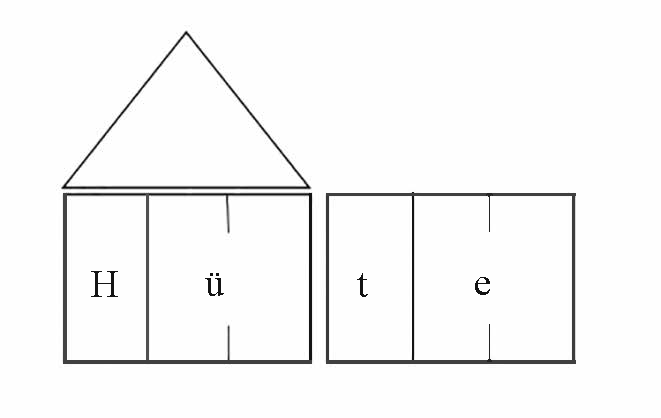
\includegraphics[width=0.5\textwidth]{figures/Huete.pdf}
    \caption{Darstellung der Silbenstruktur des Wortes \textit{Hüte} nach Röber. Die erste Silbe hat einen gespannten Vokal und ist offen.}
    \label{fig:SAMHuete}
\end{figure}

\begin{figure}
    \centering
    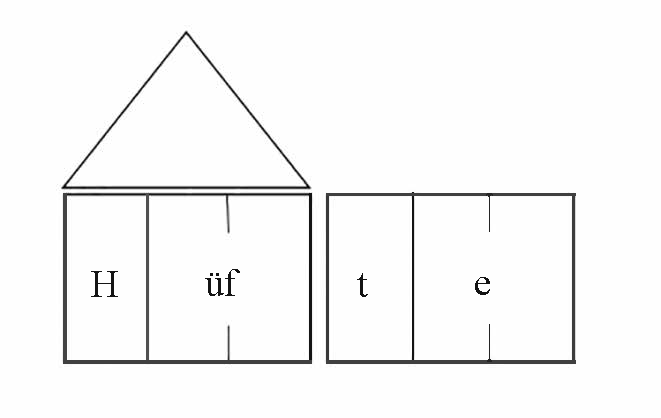
\includegraphics[width=0.5\textwidth]{figures/Huefte.pdf}
    \caption{Darstellung der Silbenstruktur des Wortes \textit{Hüfte} nach Röber. Die erste Silbe hat einen ungespannten Vokal und ist geschlossen.}
    \label{fig:SAMHuefte}
\end{figure}

Betonte Silben werden als Haus mit Dach dargestellt, unbetonte als Garage ohne Dach. Röber unterscheidet bei den betonten Silben zwei Silbentypen, die offene Silbe mit langem, gespannten Vokal (\textit{Hüte}-Typ, Abbildung~\ref{fig:SAMHuete}) und die geschlossene Silbe mit Kurzvokal (\textit{Hüfte}-Typ, Abbildung~\ref{fig:SAMHuefte}). 

Das Häusermodell kann die Unterscheidung zwischen gespannten und ungespannten Vokalen beim Lesen unterstützen und dadurch Leseaussprachen\is{Leseaussprache} wie \textipa{[\textprimstress hy:f.te:]} vermeiden helfen. Der Vokal im Haus mit Dach wird gespannt gesprochen, wenn er das große Zimmer im Haus allein bewohnt (\textit{Hüte}-Haus). Er wird ungespannt gesprochen, wenn er sich dieses Zimmer mit einem Konsonanten teilen muss (\textit{Hüfte}-Haus).\footnote{Man kann hier erkennen, warum das Modell mit Zweisilbern arbeitet. Diese Regularität gilt nämlich überhaupt nur für Zweisilber. Das Wort \textit{Hut} kann man nur unter Annahme einer weiteren Position für einen Konsonanten nach Langvokal analysieren, cf. \citet[166]{Roeber2013}.} Die Vokale der Garage werden reduziert gesprochen, meist entweder \textipa{[@]} oder \textipa{[5]}.

Für das Silbengelenk nimmt Röber einen weiteren Häusertyp an, den \textit{Hütte}-Typ. Bei diesem Häusertyp rutscht die Garage in das Haus mit Dach hinein, vgl. Abbildung~\ref{fig:SAMHuette}.

\begin{figure}
    \centering
    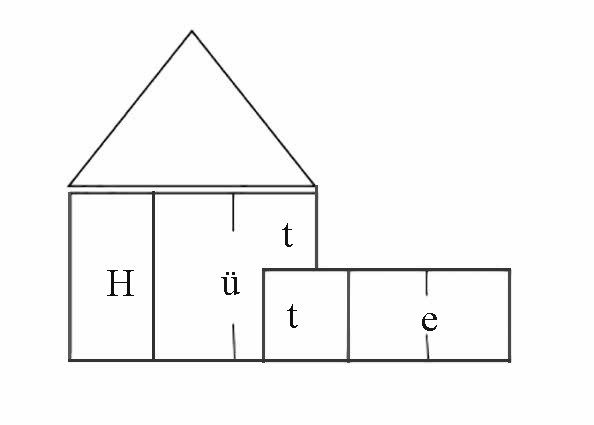
\includegraphics[width=0.5\textwidth]{figures/Huette.pdf}
    \caption{Darstellung der Silbenstruktur des Wortes \textit{Hütte} nach Röber}
    \label{fig:SAMHuette}
\end{figure}

Der Konsonant, der als Silbengelenk gesprochen wird, hat in diesem Häusertyp zwei Funktionen: Er muss als Mitbewohner im großen Zimmer zur Verfügung stehen, weil der Vokal sonst gespannt gesprochen werden würde. Außerdem muss er das erste Zimmer der zweiten Silbe besetzen. Diese Doppelfunktion wird in der Schreibung durch die Verdopplung des Konsonanten angezeigt.

Einzelne Aspekte dieses Modells haben Eingang in Lehrwerke gefunden, etwa in den Fibellehrgang \textit{ABC der Tiere} des Mildenberger-Verlags \citep[]{Handtetal2019}.

\end{Exkurs}

\subsubsection{Dehnungsschreibungen}
\label{AbschnittDehnungsh}
\is{Dehnungsschreibung}

Während die Konsonantenverdopplung -- wenn man sie als Signal für ein Silbengelenk interpretiert -- sehr systematisch ist, sind die Dehnungsschreibungen deutlich schwieriger über Regeln zu fassen. Im Deutschen existieren zwei Formen der Dehnungsmarkierung: das \textit{stumme h} und der \textit{Doppelvokal}. 

Schreibungen mit \is{Doppelvokal}Doppelvokal kommen etwa in folgenden Wörtern vor: \textit{Saat, Beet, Boot, Saal, Meer}. Einige dieser Schreibungen kann man dadurch begründen, dass Wörter von gleichlautenden anderen Wörtern unterschieden werden sollen, etwa \textit{mehr -- Meer}, vgl. auch Abschnitt~\ref{sec:Homographievermeidungsprinzip}. Abgesehen davon sind Doppelvokalschreibungen nur schwer durch Regeln zu fassen und müssen als \gqq{Merkwörter}\is{Merkwort} betrachtet werden. Doppelvokale stehen laut einer älteren Ausgabe der \citet[73--75]{Duden2016} vor allem bei einsilbigen Wörtern in offenen Silben, \zB in \textit{Fee, See}, sowie bei Zweisilbern, deren zweite Silbe mit <l, r, s> oder <t> beginnt: \textit{Meere, Aale}.

Im Gegensatz zu den recht unregelmäßigen Doppelvokalen\is{Doppelvokal} folgen die \textit{h}-Schreibungen\is{silbentrennendes h}\is{Dehnungs-h} einigen Gesetzmäßigkeiten, die im Folgenden diskutiert werden. Zunächst muss bei den h-Schreibungen zwischen dem sogenannten \textit{silbentrennenden h} (auch: silbeninitiales \textit{h}) und dem \textit{echten Dehnungs-\textit{h}} unterschieden werden. Das silbentrennende \textit{h} wird nämlich fast durchgängig geschrieben, während das Dehnungs-\textit{h} nur unter bestimmten Umständen geschrieben wird, die weiter unten genauer erläutert werden. 


Ein silbentrennendes \textit{h} trennt zwei vokalische Kerne. Es wird also immer dann gesetzt, wenn lautlich zwei Vokale aufeinandertreffen. Abbildung~\ref{Silbenstruktur_Muehe} zeigt die Silbenstruktur von \textit{Mühe}, Abbildung~\ref{Silbenstruktur_Muehle} die von \textit{Mühle}. Der wesentliche Unterschied liegt in der Besetzung des Onsets der zweiten Silbe.

\begin{figure}[!htbp]
  \centering
  \begin{forest}
  [Wort
      [σ, calign=last
        [Onset, ake
          [X
          [\textipa{m}]
          ]
        ]
      [Reim, calign=first
          [Nukleus, ake
            [X, name=X1 [,phantom ] 
                [\textipa{y:}, name=Y ]
            ]
            [X, name=X2 [,phantom ] 
            ]
          ]
        \draw (X1.south) -- (Y.north);
        \draw (X2.south) -- (Y.north);
          [Koda
      ]
      ]
      ]
      [σ, calign=last
      [\textcolor{darkgray}{Onset}
        ]
        [Reim
          [Nukleus, ake
            [X
            [\textipa{@}]
            ]
          ]
          [Koda
          ]
        ]
      ]
    ]
  \end{forest}
  \caption{Konstituentenanalyse von \textit{Mühe}: Der Onset der zweiten Silbe ist leer. Das geschriebene <h> ist also ein silbentrennendes h.}
  \label{Silbenstruktur_Muehe}
\end{figure}



Bei \textit{Mühe} sind die Koda der ersten Silbe und der Onset der zweiten Silbe leer. Dadurch treffen die beiden vokalischen Kerne direkt aufeinander. In der Schreibung dient das zwischen den Vokalen eingefügte <h> der optischen Trennung der Silben als Erleichterung beim Lesen.


\begin{figure}[!htbp]
  \centering
  \begin{forest}
  [Wort
      [σ, calign=last
        [Onset, ake
          [X
          [\textipa{m}]]
        ]
       [Reim, calign=first
          [Nukleus, ake
            [X, name=X1 [,phantom ] 
                [\textipa{y:}, name=Y ]
            ]
            [X, name=X2 [,phantom ] 
            ]
          ]
        \draw (X1.south) -- (Y.north);
        \draw (X2.south) -- (Y.north);
          [Koda
      ]
      ]
      ]
      [σ, calign=last
      [Onset, ake
          [X[\textipa{l}]
          ]
        ]
        [Reim
          [Nukleus, ake
            [X[\textipa{@}]]
          ]
          [Koda
          ]
        ]
      ]
    ]
  \end{forest}
  \caption{Konstituentenanalyse von \textit{Mühle}: Der Onset der zweiten Silbe ist besetzt und trennt die beiden vokalischen Kerne. Das geschriebene <h> ist also ein Dehnungs-\textit{h}.}
  \label{Silbenstruktur_Muehle}
\end{figure}



Bei \textit{Mühle} ist der Onset der zweiten Silbe mit \textipa{/l/} besetzt. Die vokalischen Kerne werden also durch einen Konsonanten separiert. In der Schreibung trennt das \textit{h} also nicht die vokalischen Kerne. Es handelt sich deshalb um ein echtes Dehnungs-\textit{h}, welches nur die Funktion hat, die Länge des Vokals in der ersten Silbe anzuzeigen.

\subsubsubsection{Silbentrennendes \textit{h}}\is{silbentrennendes h}

Während das Dehnungs-\textit{h} statistisch gesehen meistens nicht gesetzt wird (es gibt viele Wörter mit Langvokalen ohne \textit{h}, \zB \textit{treten, baden, Masern} usw.), wird das silbentrennende \textit{h} fast immer geschrieben: \textit{sehen, gehen, Wehe, fliehen, Flöhe, Kühe, Ruhe}. Eine Ausnahme bilden Wörter mit Diphthongen\is{Diphthong} als silbischem Kern: \textit{bauen, teuer, Reue, schlaue, klauen}. \citet[225]{FuhrhopPeters2013} führen als Begründung an, dass die Silben durch die Diphthonge optisch lang genug sind, so dass man erkennen kann, dass es sich um zwei Silben handelt. Das ist anders bei \textit{sehen} vs. \textit{*seen}, welches auch als Einsilber gelesen werden kann. Eine Ausnahme unter den Diphthongen ist das <ei>, nach welchem häufig doch ein silbentrennendes \textit{h} steht: \textit{leihen, Geweihe},\footnote{Wir geben hier den Plural als Beispiel an. Der Singular \textit{Geweih} wird zwar auch mit \textit{h} geschrieben, allerdings handelt es sich hier nicht um eine \textit{h}-Schreibung nach dem silbischen Prinzip, sondern um eine nach dem morphologischen Prinzip. \textit{Geweih} wird mit \textit{h} geschrieben, weil \textit{Geweihe} mit \textit{h} geschrieben wird.} aber auch: \textit{Feier}.

Einige erwachsene Schreiberinnen und Schreiber sind der Meinung, dass man das silbentrennende \textit{h} hören kann. Auch in Lehrmaterialien findet man diese Fehlinformation. Folgendes Zitat ist dem Zebra-Arbeitsheft für die Klasse 6 von Klett entnommen \citep[22]{Bambergetal2018}. 

\begin{quote}
Das \textit{h} am Ende eines Wortstammes nennt man \textit{silbentrennendes h}. Du kannst es hören, wenn du das Wort weiterschwingst\footnote{\gqq{Weiterschwingen} bedeutet, das Wort um eine Silbe zu verlängern.}: Schuh -- Schuhe, blüht -- blühen.
\end{quote}

Genauso könnte man Wörter wie \textit{baut} weiterschwingen zu \textit{*bauhen} oder \textit{ausgesät} zu \textit{*aussähen}. Das silbentrennende \textit{h} kann man tatsächlich \textit{nicht} hören, denn es wird -- auch in der Standardaussprache -- nicht gesprochen.  Es ist ein orthografischer Silbentrenner, der allein in der geschriebenen Sprache, also für das Auge existiert und keine lautliche Entsprechung hat.

\subsubsubsection{Echtes Dehnungs-\textit{h}}\is{Dehnungs-h}
Beim echten Dehnungs-\textit{h} steht ein weiterer Konsonant zwischen den vokalischen Kernen, \zB in \textit{Mühle, Fehler} oder zwischen dem vokalischen Kern und dem Ende des Wortes, \zB in \textit{Jahr, zahm}. Auf den ersten Blick wird dieses Dehnungs-\textit{h} recht willkürlich mal gesetzt und mal nicht. In Tabelle~\ref{DehnungshSono} sind Beispielwörter aufgelistet. Alle Wörter sind Trochäen (vgl. Abschnitt~\ref{section:betonte_unbetonte_Silben}) und haben einen Langvokal in der ersten Silbe. Die zweiten Silben haben besetzte Onsets. Warum werden die Wörter in der ersten Spalte alle mit Dehnungs-\textit{h} geschrieben, die Wörter in der zweiten Spalte jedoch nicht? Beachten Sie bitte die Konsonanten, die dem Dehnungs-\textit{h} bzw. dem Vokal folgen.

\begin{table}
\caption{\label{DehnungshSono} Wörter mit Langvokal, die mit Dehnungs-\textit{h} (links) und ohne Dehnungs-\textit{h} (rechts) geschrieben werden}
\begin{tabular}{ll}\lsptoprule
mit Dehnungs-\textit{h}&ohne Dehnungs-\textit{h}\\\midrule
\textit{fehlen}& \textit{Fete}\\
\textit{Fohlen} & \textit{Vogel}\\
\textit{Sahne} & \textit{Sage}\\
\textit{zählen} & \textit{Nagel}\\
\textit{nehmen} & \textit{häkeln} \\
\textit{zahm} & \textit{Tag}\\
\textit{Rahmen} & \textit{rasen}\\
\textit{föhnen} & \textit{Möwe}\\
\textit{wehren} & \textit{Wesen}\\\lspbottomrule
\end{tabular}
\end{table}

Der Konsonant, der dem Dehnungs-\textit{h}\is{Dehnungs-h} in den Wörtern in der linken Spalte folgt, ist immer ein \is{Sonorant}Sonorant, bei \textit{fehlen} und \textit{Fohlen} ein \textipa{/l/}, bei \textit{Sahne} ein \textipa{/n/} usw. In den Beispielen ohne Dehnungs-\textit{h} steht an der Stelle ein \is{Obstruent}Obstruent, bei \textit{Fete} ein \textipa{/t/}, bei \textit{Vogel} und \textit{Sage} ein \textipa{/g/} usw. Laut \citet[225]{FuhrhopPeters2013} dient das Dehnungs-\textit{h} hier der Leserin oder dem Leser dazu, die Silbengrenze optisch besser zu erkennen, weil Sonorantengrapheme oft keine Ober- und Unterlängen haben und die Silbengrenze deshalb nicht gut markieren (vgl. Abschnitt~\ref{sec:OberUnterlängen}). Das wirkt sich auch auf die Schreibung der Einsilber aus, weil diese durch Flexion mehrsilbig werden können, \zB \textit{zahme}. Die Regel, die man aus diesen Überlegungen ableiten kann, lautet: \textit{Vor Obstruenten steht in der Regel kein Dehnungs-\textit{h}}.

Bei Sonoranten\is{Sonorant} steht häufig ein Dehnungs-\textit{h}: \textit{Sohle, kehren, lahm}. Es lassen sich aber zahlreiche Gegenbeispiele finden: \textit{Schule, Schale, Qual, klar, Gram}. Im Gegensatz zu den Wörtern in Tabelle~\ref{DehnungshSono} stehen bei diesen Wörtern mehrere Buchstaben im Onset der betonten Silbe. Die Silben haben also \textit{graphematisch komplexe Onsets}\is{Onset!graphematisch komplex}. \citet[225]{FuhrhopPeters2013} zufolge wird hier auf eine Dehnungsmarkierung verzichtet, weil die Silbe optisch sonst zu lang werden würde und beim flüssigen Lesen nicht mehr zweifelsfrei als eine einzige Silbe erkannt werden könnte: \textit{*Schuhle, *Schahle, *Quahl, *klahr, *Grahm}.

Zu einer anderen Gruppe von Gegenbeispielen gehören Wörter mit dem Onset <t>: \textit{Tal, Tor, Tür, Ton}. Diese Schreibungen sind ein Resultat der Orthografiereform von 1902. Bis dahin wurden die Wörter \textit{Thal, Thor, Thür, Thon} geschrieben und hatten damit komplexe Onsets \citep[166]{Roeber2013}.

Die zweite Regel zum Dehnungs-\textit{h} kann man also wie folgt formulieren: \textit{Vor Sonoranten steht ein Dehnungs-\textit{h}, wenn der Onset der entsprechenden Silbe einfach und nicht <t> ist.}


\begin{Exkurs}{Dehungs-\textit{h}: Implizite und explizite Regelbildung}

\noindent Den meisten kompetenten Schreiberinnen und Schreibern des Deutschen ist nicht bewusst, dass das Dehnungs-\textit{h} vor allem vor Sonoranten steht. Trotzdem können sie die allermeisten Wörter korrekt schreiben. Mehr noch: Bei Wörtern, die ihnen bisher unbekannt waren, haben sie in der Regel ein klares Gefühl dafür, ob die Wörter mit Dehnungs-\textit{h} geschrieben werden sollten oder nicht. Wenn man sich vorstellt, man würde ein neuartiges Produkt namens \textipa{[\textprimstress fe:.g@l]} oder \textipa{[\textprimstress go:.t5]} kennenlernen, dann würde man eher die Schreibung \textit{Fegel} oder \textit{Goter} erwarten als \textit{Fehgel} oder \textit{Gohter}. Ein Produkt namens \textipa{[\textprimstress fe:.n@l]} oder \textipa{[\textprimstress go:.m5]} hingegen würde man eher \textit{Fehnel} oder \textit{Gohmer} schreiben als \textit{Fenel} oder \textit{Gomer}. Viele Schreiberinnen und Schreiber haben die Regeln zum Dehnungs-\textit{h} \textit{implizit} erworben, d.\,h. ohne dass sie eine Regel dazu formulieren können oder jemals eine Regel kennengelernt haben.\is{implizite Regelbildung}

Wenn man die Regeln anwenden kann, ohne sie explizit formulieren zu können, ist die Frage berechtigt: Müssen Lehrkräfte die Regeln zum Dehnungs-\textit{h} kennen? Um korrekt schreiben zu können, muss man die Regeln nicht kennen. Man braucht sie jedoch, um erkennen zu können, dass ein Kind, welches in der fünften Klasse plötzlich \textit{*Schuhle} schreibt, nicht auf einmal alles verlernt hat, sondern -- im Gegenteil -- mehr als vorher weiß. Dieses Kind hat die oben genannte Sonoranten-Regel verinnerlicht. Damit weiß das Kind mehr als ein Kind, welches ebenso falsch \textit{*Rahsen} schreibt. Wenn Lernende \textit{*Schuhle} schreiben, könnte der nächste Schritt sein, sich die Schreibung von Wörtern mit komplexen Onsets anzusehen. 

Wissen zu den Regeln des Dehnungs-\textit{h} ermöglicht außerdem das Erkennen von echten Ausnahmen (Merkwörtern)\is{Merkwort}. Wörter wie \textit{Düne} oder \textit{Runen} sind nur für Erstklässler \gqq{einfach}. Diese Schreibungen sind nämlich nach den oben diskutierten Regeln irregulär. Irreguläre Formen werden durch häufigen Gebrauch leicht konserviert. \citet[115]{croft:2003} zeigt das für grammatische Formen und man kann davon ausgehen, dass dies auch für Schreibungen gilt. So sollte das sehr häufige Wort \textit{Name} eigentlich mit Dehnungs-\textit{h} geschrieben werden. 

Der Erwerb der Rechtschreibung ist generell stark geprägt von impliziter Regelbildung: Lernende leiten die Regeln unbewusst aus dem Material ab, mit welchem sie konfrontiert werden. Hilfreich ist es dabei, wenn das Material so ausgewählt wurde, dass die Lernenden die Regeln auch tatsächlich erkennen können (indem beispielsweise auf die \textit{Düne} und die \textit{Runen} vorerst verzichtet wird).

Die Lernwortschätze\is{Lernwortschatz}, die in einigen Bundesländern für den Rechtschreibunterricht vorgegeben werden, enthalten einerseits häufige Wörter, die möglicherweise irregulär geschrieben werden, andererseits aber auch sogenannte \textit{Modellwörter}\is{Modellwort} -- also Wörter, an denen Lernende erkennen können, nach welchen Regeln die meisten Wörter geschrieben werden. Die irregulären -- aber häufigen -- Wörter können den Blick auf das Regelhafte in der deutschen Orthografie manchmal verstellen. 

\is{explizite Regeln}Trotz des meist impliziten Erwerbs der Dehnungsschreibungen gibt es Lehrwerke, die mit expliziten Regeln arbeiten, \zB ABC der Tiere \citep{Mildenbergero.J.}. Die Kinder werden in diesem Lehrwerk aufgefordert, das Dehnungs-\textit{h} nur vor \textit{l, m, n, r} (den Sonoranten) zu setzen und es bei \gqq{Doppelstartern} (Wörtern mit komplexen Onsets) und Wörtern mit dem Onset \textit{t} wegzulassen.

\end{Exkurs}


\begin{Exkurs}{Fremdwortschreibung}\is{Fremdwortschreibung}

\noindent Schon zu Beginn des Schriftspracherwerbs werden Lernende häufiger mit Wörtern konfrontiert, die nicht nach den oben beschriebenen Regeln geschrieben werden, weil sie Fremdwörter sind:

\begin{itemize}
    \item \textit{Kino, Pirat, Mandarine, Lawine} (statt nach den Graphem-Phonem-Korres\-pondenzen \textit{*Kieno, *Pierat, *Mandariene, *Lawiene})
    \item \textit{Kamel, Regal} (statt nach den Regeln zum Dehnungs-\textit{h} \textit{*Kamehl, *Regahl})
\end{itemize}

Für das Betrachten gerade dieser Wörter im Unterricht gibt es meist gute Gründe. Die Wörter sind möglicherweise häufig im kindlichen Wortschatz oder sie sind generell häufig oder sie werden etwa im Sachunterricht benötigt. 

Zu Beginn des Schriftspracherwerbs finden Kinder diese Wörter sehr einfach zu schreiben, denn typische Schwierigkeiten wie das Dehnungs-\textit{h} oder die <ie>-Schreibung treten bei diesen Wörtern nicht auf. Schreibungen wie \textit{Kamehl} oder \textit{Pierat} findet man erst, wenn die Kinder das Dehnungs-\textit{h} kennen und die \textipa{/i/}--<ie>-Korrespondenz verstanden haben. 

Soll man diese Wörter nun als Merkwörter\is{Merkwort} alle auswendig lernen? \citet{Bredel2011} bietet ein relativ einfaches Verfahren an, um zumindest Fremdwörter romanischen Ursprungs am Betonungsmuster zu erkennen -- und dann eben nicht nach den deutschen Regeln zu schreiben. Während einfache Erbwörter und Lehnwörter (eingedeutschte Wörter) normalerweise Trochäen\is{Trochäus}\is{Erbwort}\footnote{Erbwörter, bei denen die erste Silbe nicht betont ist, haben in der Regel ein Präfix: \textit{Verband, Gelände, entgleisen}} sind, sind Fremdwörter romanischen Urspungs normalerweise nicht auf der ersten Silbe betont (\textit{Kamel, Regal, Mandarine, Pirat}). Die Schreibung dieser nicht-trochäischen Wörter weicht auf folgende Art und Weise regelhaft von der Schreibung der Erb- und \is{Lehnwort}Lehnwörter ab:

\begin{itemize}
    \item Es gibt kein silbentrennendes und kein Dehnungs-\textit{h}.
    \item \textipa{[i]} wird <i> geschrieben.
\end{itemize}

Die Silbengelenksschreibung bleibt jedoch erhalten: \textit{Krawatte, Perücke}.

\end{Exkurs}


\subsection{Morphologisches Prinzip}
\label{sec:MorphPrin}
\is{morphologisches Prinzip}

Viele Aspekte der Schreibungen \textit{Fall} und \textit{Fälle} sind phonographisch:
\begin{itemize}
    \item Dem Laut \textipa{[f]} entspricht das Graphem <F>.
    \item Dem Laut \textipa{[l]} entspricht eine l-Schreibung.
    \item In \textit{Fall} entspricht dem \textipa{[a]} das <a>.
\end{itemize}

Mittels des silbischen Prinzips kann man außerdem erklären, warum \textit{Fälle} mit Doppelkonsonant geschrieben wird: Das \textipa{[l]} ist ein Silbengelenk\is{Silbengelenk}. Dass \textit{Fall} mit Doppelkonsonant geschrieben wird, kann man nicht anhand des silbischen Prinzips erklären, denn in diesem Wort gibt es gar kein Silbengelenk. \textit{Fall} wird nur mit <ll> geschrieben, weil \textit{Fälle} mit <ll> geschrieben wird.\footnote{Dass der Grund für das <ll> ursächlich nicht der Kurzvokal ist, kann man erkennen, wenn man es mit Wörtern vergleicht, zu denen es keine verwandten Wörter mit Silbengelenk gibt, etwa Präpositionen und Subjunktionen wie \textit{mit, bis, um, an}. Alle diese Wörter haben Kurzvokale, werden aber nur mit einem Konsonanten nach dem Vokal geschrieben.} Auch die <ä>-Schreibung in \textit{Fälle} ist morphologisch begründbar: Sie zeigt die Vewandtschaft zu \textit{Fall}. Das morphologische Prinzip (auch: Stammprinzip\is{Stammprinzip}) kann man wie folgt fassen (\cite[41]{GallmannSitta1996}, \cite[913f]{Duden2022}, \cite[239]{FuhrhopPeters2013}, \cite[505]{Schaefer2018_3Aufl}):


\begin{Definition}{Morphologisches Prinzip (Morphemkonstanz)}\label{def:morphPrinzip}

\noindent Morpheme werden in allen morphologisch verwandten Stämmen gleich oder ähnlich geschrieben.

\end{Definition}


Nach dem morphologischen Prinzip schreibt man beispielsweise das Wort \textit{Hände} mit <ä>, damit die Verwandtschaft zu \textit{Hand} erkennbar ist. Aber auch bei \textit{Hand} handelt es sich um eine morphologische Schreibung: das <d> am Ende ist nicht phonographisch und verweist auf die Verwandtschaft mit \textit{Hände}. Das Beispiel zeigt, dass morphologische Schreibungen nicht nur bei komplexeren Wörtern vorkommen, die von einfacheren abgeleitet wurden, sondern auch bei einfachen Wörtern, die die Basis für komplexere Wörter sind.

Der Erwerb der morphologischen Schreibungen setzt in der Regel erst nach dem Erwerbsbeginn der silbischen Schreibungen ein (vgl. \zB Modell nach Dehn, zitiert in \cite[Abschnitt 2.4]{Thome1999}, Modell nach \cite{May2013}). Das liegt daran, dass die Einheiten, die man für die Schreibung betrachten muss, größer werden. Bei Schreibungen nach dem phonographischen und silbischen Prinzip muss man nur die Eigenschaften des Wortes analysieren, welches man schreiben will. Um morphologische Schreibungen zu verstehen, muss man wissen, dass Wörter morphologisch miteinander verwandt sind und die Schreibung der Wortfamilie betrachten. Außerdem muss das mentale Lexikon\is{mentales Lexikon} relativ groß sein, damit man verwandte Wörter überhaupt kennt. 

Im Folgenden werden vier häufige Arten von morphologischen Schreibungen diskutiert: die <ä/äu>-Schreibungen, die Schreibung auslautverhärteter Konsonanten, die Schreibung von \textipa{/K/}-Vokalisierungen und die Schreibung von Konsonanten, bei denen eine \textipa{/g/}-Spirantisierung stattgefunden hat.

\subsubsection{<ä/äu>-Schreibungen}\label{subsec:ääuSchreibungen}\is{ae/aeu-Schreibungen@ä/äu-Schreibungen}

Schreibungen wie etwa \textit{Fälle, Bänder, Bäcker, Häuser, Läuse, Bäume} signalisieren eine Verwandtschaft mit Wörtern, die mit <a> oder <au> geschrieben werden: \textit{Fall, Band, backen, Haus, Laus, Baum}. 
 
In der Regel lernen Kinder als erste Möglichkeit zur Ermittlung der \textit{ä}-Schreibung die Rückführung auf den Singular kennen. In den Aufgaben der \textit{Rechtschreibbox} (\cite[29/1]{Lessmann2009}, \cite{Lessmann2013}), ist beispielsweise vorgesehen, dass die Lernenden die Schreibung der Wörter \textit{Räder, Gläser, Nägel, Äpfel} und \textit{Kämme} ermitteln, indem sie sie auf den Singular zurückführen (\textit{Rad, Glas, Nagel, Apfel, Kamm}). Bei einigen Wörtern ist das Erkennen eines morphologischen Zusammenhangs allerdings deutlich schwieriger (\textit{nächste} muss man etwa auf \textit{nach} zurückführen, \textit{ändern} auf \textit{anders}). Deshalb kann der Erwerb der morphologischen Schreibungen mehrere Jahre beanspruchen.
 
Die große Mehrheit der Wörter mit <ä> und <äu> sind die gerade diskutierten morphologische Schreibungen. Es gibt jedoch einige Wörter, die aus historischen Gründen\is{historische Schreibungen} mit <ä> oder <äu> geschrieben werden, \zB weil es mal verwandte Wörter gab, die mit <a> oder <au> geschrieben wurden, diese aber nicht mehr gebräuchlich sind. Das Wort \textit{Knäuel} war beispielsweise mal eine Nebenform von \textit{Knauel} \citep{Grimm2020}. Zu den Wörtern, deren Schreibung synchron nicht mehr als morphologische Schreibung gelten kann, weil keine verwandten Wörter mit <a/au> (mehr) existieren, gehören \textit{Bär, Käse, Gewähr, März, Säge, Käfer, Säule, Knäuel, sich sträuben, sich räuspern}. Im Unterschied zu Wörtern wie \textit{Räder, Gläser} kann man die Schreibung hier nicht ableiten. Man muss sich diese Schreibungen merken.\footnote{Außerdem gibt es noch eine weitere Gruppe von Wörtern mit <ä>, bei denen das <ä> aber eine ganz andere Funktion hat: \textit{Aktionär, subsidiär, Militär, populär, legendär}. Auch diese Schreibungen sind keine morphologischen Schreibungen. Das Betonungsmuster dieser Wörter weicht vom für das Deutsche typischen Trochäus\is{Trochäus} ab. Das <ä> kennzeichnet bei diesen Wörtern die betonte Silbe. Würde man \zB \textit{*Aktioner} statt \textit{Aktionär} schreiben, würde die 2. Silbe betont werden und die eigentlich betonte letzte Silbe zur Reduktionssilbe werden \citep[231f]{FuhrhopPeters2013}.}
 

\subsubsection{Schreibung auslautverhärteter Konsonanten}\is{Auslautverhärtung}

In der Rechtschreibbox von \citet[32/2]{Lessmann2009} gibt es eine Übung, bei der Lernende die Schreibung der Wörter \textit{Hund, Pirat, Mund, Wald, Nacht} und \textit{Feind} ermitteln sollen, indem sie den Plural bilden. Anhand der Aussprache des Konsonanten \textipa{[d]} oder \textipa{[t]} in der Pluralform sollen die Lernenden einen Rückschluss auf die Schreibung des Wortes im Singular ziehen, wo es keinen lautlichen Unterschied am Wortende gibt. Um die Singularformen richtig zu schreiben, muss man also ein anderes Wort analysieren; es handelt sich bei Schreibungen wie \textit{Hund} usw. deshalb um morphologische Schreibungen. Im Singular werden all diese Wörter aufgrund der Auslautverhärtung mit einem stimmlosen Konsonanten gesprochen, die Schreibung weicht hier von der Lautung ab.

Konsonanten, die im Deutschen auslautverhärtet werden, behalten in ihrer geschriebenen Form also den in der phonologischen Repräsentation\is{phonologische Repräsentation} angelegten stimmhaften Konsonanten (vgl. Abschnitt~\ref{section:phonProzesse}). Tabelle~\ref{tab:SchreibungAuslautverhaertung} enthält dazu einige Beispiele.

\begin{table}
\caption{\label{tab:SchreibungAuslautverhaertung} Lautliche und graphematische Repräsentationen von Wörtern mit auslautverhärteten Konsonanten}
\begin{tabular}{lll}\lsptoprule
Phonologische Repräsentation & Lautung & Schreibung\\\midrule
\textipa{/li:d/} & \textipa{[li:t]} & <Lied>\\
\textipa{/\textprimstress hand.lIç/}& \textipa{[\textprimstress hant.lIç]          } & <handlich>\\
\textipa{/gra:z/} & \textipa{[gra:s]} & <Gras>\\\lspbottomrule
\end{tabular}
\end{table}

Im ersten Beispiel, \textit{Lied}, wird das in der phonologischen Repräsentation vorhandene finale \textipa{/d/} in die Schreibung übernommen, obwohl \textipa{[t]} gesprochen wird. Das zweite Beispiel, \textit{handlich}, zeigt, dass die Auslautverhärtung auch nichtfinal stattfinden kann. Am dritten Beispiel, \textit{Gras}, kann man sehen, dass die Auslautverhärtung nicht nur Plosive\is{Plosiv}, sondern viel allgemeiner Obstruenten (also auch Frikative\is{Frikativ}) betrifft (vgl. Abschnitt~\ref{sec:Auslautverhaertung}). 

Bei der Auslautverhärtung handelt es sich um einen sprachspezifischen phonologischen Prozess. Außer im Deutschen gibt es diesen Prozess \zB auch im Russischen und Türkischen, aber nicht im Englischen und Französischen (vgl. Abschnitt~\ref{sec:Auslautverhaertung}). Beispiel (\ref{EnglischAuslaute}) zeigt, dass sich im Englischen zwei Wörter durch einen finalen stimmhaften bzw. stimmlosen Laut unterscheiden können:

\ea \label{EnglischAuslaute}
\ea \label{ea:EnglischAuslaute1} bag \textipa{[b\ae g]} \gqq{Tasche}
\ex \label{ea:EnglischAuslaute2} back \textipa{[b\ae k]} \gqq{Rücken}
\z
\z

Im Deutschen ist dies nicht möglich; solche Wörter wären Homophone\is{Homophon},\footnote{Homophone sind gleichklingende Wörter.} vgl. etwa \textit{Rad} und \textit{Rat}, die beide \textipa{[Ka:t]} gesprochen werden. Das Französische ist vergleichbar mit dem Englischen:

\ea \label{FranzoesischAuslaute}
\ea \label{ea:FranzoesischAuslaute1} (je) monte \textipa{[m\~Ot]} \gqq{ich steige}
\ex \label{ea:FranzoesischAuslaute2} (le) monde \textipa{[m\~Od]} \gqq{die Welt}
\z
\z

Englisch und Französisch haben also keine Auslautverhärtung\is{Auslautverhärtung}. Die Sprachen \textit{mit} Auslautverhärtung unterscheiden sich im Hinblick darauf, ob sich die Schreibung an der auslautverhärteten Variante oder an der phonologischen Repräsentation orientiert. Während das Türkische die auslautverhärtete Variante schreibt, folgt die Schreibung im Russischen und Deutschen der phonologischen Repräsentation. Beispiel (\ref{ea:TuerkischAuslautverhaertung1}) zeigt ein türkisches Wort, bei dem ein stimmloses \textipa{[p]} als <p> geschrieben wird. Im verwandten Wort in Beispiel (\ref{ea:TuerkischAuslautverhaertung2}) wird der Plosiv nicht auslautverhärtet und wird deshalb <b> geschrieben.


\ea \label{TuerkischAuslautverhaertung}
\ea \label{ea:TuerkischAuslautverhaertung1} kitap \textipa{[kitap]} \gqq{das Buch}
\ex \label{ea:TuerkischAuslautverhaertung2} kitabim \textipa{[kitabim]} \gqq{mein Buch}
\z
\z

 
Das russische Beispiel (\ref{ea:RussischAuslautverhaertung1}) zeigt ein Wort, bei dem der finale Laut auslautverhärtet wird. In der Schreibung ist dies nicht sichtbar. Der Stamm wird genauso wie in Beispiel (\ref{ea:RussischAuslautverhaertung2}) -- wo keine Auslautverhärtung erfolgt --  mit <д>, der kyrillischen Entsprechung von \textipa{/d/} geschrieben.


\ea \label{RussischAuslautverhaertung}
\ea \label{ea:RussischAuslautverhaertung1} гoрод \textipa{[\textprimstress gO.r@t]} \gqq{Stadt}
\ex \label{ea:RussischAuslautverhaertung2} гoродa  \textipa{[g@.r5\textprimstress da]} \gqq{Städte}
\z
\z


Die Schreibung der Auslautverhärtung im Deutschen, genauso wie im Russischen, zählt zu den morphologischen Schreibungen, weil dadurch verwandte Stämme gleich geschrieben werden, unabhängig davon, ob auslautverhärtet wird oder nicht, vgl. Beispiele (\ref{ea:DeutschAuslautverhaertung1}), (\ref{ea:DeutschAuslautverhaertung3}) und (\ref{ea:DeutschAuslautverhaertung4}) vs. Beispiel (\ref{ea:DeutschAuslautverhaertung2}):

\ea \label{DeutschAuslautverhaertung}
\ea \label{ea:DeutschAuslautverhaertung1} Kind \textipa{[\textprimstress kInt]}
\ex \label{ea:DeutschAuslautverhaertung2} Kinder  \textipa{[\textprimstress kIn.d5]}
\ex \label{ea:DeutschAuslautverhaertung3} kindlich  \textipa{[\textprimstress kInt.lIç]}
\ex \label{ea:DeutschAuslautverhaertung4} Kindchen  \textipa{[\textprimstress kInt.ç@n]}
\z
\z


\begin{Exkurs}{Die Verlängerungsprobe (\gqq{Weiterschwingen})}\is{Verlängerungsprobe}

\noindent In der Schule wird zum Erkennen von morphologischen Schreibungen ein Verfahren unterrichtet, welches \textit{Verlängerungsprobe} oder auch \textit{Weiterschwingen} genannt wird. Das Beispiel von Lessmann zu Beginn des Abschnittes demonstriert dieses Verfahren. Bei der Verlängerungsprobe versucht man, das Wort so zu verändern, dass der Konsonant, der in der Koda steht (bei \textit{Kind} das gesprochene \textipa{[t]}), in den Onset der nächsten Silbe übergeht: \textipa{[\textprimstress kIn.d5]} \textit{Kinder}. Konsonanten in dieser Position (im Onset) werden nicht auslautverhärtet und geben damit Aufschluss über die phonologische Repräsentation und so über die Schreibung.

Es ist leicht ersichtlich, dass nicht jede Verlängerung diesem Kriterium genügt. Wenn man von \textit{Kind kindlich} ableitet, ist das Wort zwar länger, gibt aber immer noch keinen Aufschluss über die Schreibung, weil der auslautverhärtete Konsonant immer noch in der Koda steht und deshalb wieder auslautverhärtet wird. Wenn man \textit{kindlich} schreiben möchte, müsste man das Wort \textit{Kinder} betrachten. Das ist sogar kürzer, so dass der Terminus \textit{Verlängerungsprobe} irreführend ist und deshalb auch häufig von \textit{Ableiten} gesprochen wird.

Das Verfahren der Verlängerungsprobe, das kompetenten Schreiberinnen und Schreibern so einfach erscheint, ist also nicht ganz einfach zu erlernen. Die meisten Lehrwerke bieten ein schrittweises Vorgehen an, bei welchem zunächst ausschließlich der Plural als Ableitungsform berücksichtigt wird und erst später das Verfahren \gqq{Erst kürzen und dann ableiten} eingeführt wird, um etwa von \textit{kindlich} auf \textit{Kind} und dann auf \textit{Kinder} zu kommen \citep{Lessmann2009}.
\end{Exkurs}

\subsubsection{Schreibung von Wörtern mit \textipa{/K/}-Vokalisierung}\is{R-Vokalisierung@\textipa{/K/}-Vokalisierung}

In Abschnitt~\ref{subsec:r-Vokalisierung} wurde gezeigt, dass die \textipa{/K/}-Vokalisierung ein phonologischer Prozess ist, der r-Laute in der Koda\is{Koda} betrifft. Dabei wird der r-Laut durch das tiefe Schwa\is{tiefes Schwa} ersetzt: \textit{Tor} \textipa{[to:5]} oder \textipa{[t\t*{o5}]} (vgl. Abbildung~\ref{Silbenstruktur_Tor}).
Beim Plural dieses Wortes, \textit{Tore}, steht der r-Laut im Onset der Folgesilbe und wird deshalb nicht vokalisiert (vgl. Abbildung~\ref{Silbenstruktur_Tore}).

\begin{figure}[!htbp]
  \centering
  \begin{forest}
[σ 
        [Onset, ake 
          [X [\textipa{t}]]
        ]
        [Reim 
         [Nukleus
           [X, name=ERBaum]
           [X
                [\textipa{o:}]
                {\draw[-] (.north) -- (ERBaum.south);}
            ] 
        ] 
          [\textcolor{darkgray}{Koda}, ake
            [X [\textipa{K}]]
          ]
      ] 
] 
  \end{forest}
  \caption{Konstituentenanalyse der phonologischen Repräsentation von \textit{Tor}: Der r-Laut steht in der Koda und wird dort vokalisiert. In einer phonetischen Repräsentation müsste das tiefe Schwa, das aufgrund der \textipa{/K/}-Vokalisierung entstanden ist, als Vokal im Nukleus stehen und dort zusammen mit \textipa{[o]} einen Diphthong bilden (Abbildungen~\ref{Silbenstruktur_Tier} und \ref{Silbenstruktur_Tier_vokalisiert} auf Seite \pageref{Silbenstruktur_Tier_vokalisiert}).}
  \label{Silbenstruktur_Tor}
\end{figure}




\begin{figure}[!htbp]
  \centering
  \begin{forest}
  [Wort
      [σ, calign=last
        [Onset, ake
          [X [\textipa{t}]]
        ]
      [Reim, calign=first
          [Nukleus, ake
          [X, name=ERBaum]
    [X [\textipa{o:}]
    {\draw[-] (.north) -- (ERBaum.south);}
    ]
          ]
          [Koda,
      ]
      ]
      ]
      [σ, calign=last
      [\textcolor{darkgray}{Onset}, ake
          [X [\textcolor{darkgray}{\textipa{K}}]]
        ]
        [Reim
          [Nukleus, ake
            [X [\textipa{@}]]
          ]
          [Koda
          ]
        ]
      ]
    ]
  \end{forest}
  \caption{Konstituentenanalyse von \textit{Tore}: Der r-Laut steht im Onset der zweiten Silbe und wird nicht vokalisiert.}
  \label{Silbenstruktur_Tore}
\end{figure}

Weitere Beispiele für Wörter mit \textipa{/K/}-Vokalisisierung sind \textit{aber} \textipa{[\textprimstress Pa:.b5]}, ebenso \textit{Bär} \textipa{[b\t*{E5}]} oder \textipa{[b\t*{e5}]}, \textit{Meer} \textipa{[m\t*{e5}]}, \textit{vier} \textipa{[f\t*{i5}]}, \textit{Flur} \textipa{[fl\t*{u5}]} und mit nichtfinalem \textipa{/K/}: \textit{Form} \textipa{[f\t*{O5}m]}, \textit{dort} \textipa{[d\t*{O5}t]}, \textit{Fahrt} \textipa{[f\t*{a5}t]}, \textit{Pferd} \textipa{[\t{pf}\t*{e5}t]}, \textit{fern} \textipa{[f\t*{E5}n]}.\footnote{Nach ungespanntem Vokal vokalisieren nicht alle Sprecherinnen und Sprecher (vgl. Abschnitte~\ref{subsection:Reduktionsvokale}, \ref{subsec:Diphthonge}, \ref{subsec:r-Vokalisierung}).} Wenn der r-Laut hingegen im Onset steht, wird er nicht vokalisiert: \textit{Druck} \textipa{[dKUk]}, \textit{Kreis} \textipa{[kK\t*{aI}s]}, \textit{raus} \textipa{[K\t*{aU}s]}, sondern es wird eines der r-Allophone \textipa{[r, \;R, K]} gesprochen.

Zu Beginn des Schriftspracherwerbs\is{Schriftspracherwerb}, aber auch später, versuchen Kinder, diese Wörter mit vokalisiertem \textipa{/K/} phonographisch zu schreiben, wobei aufgrund der lautlichen Nähe eine Korrespondenz zwischen \textipa{[5]} und <a> angenommen wird:

\ea \label{rVokalisierung}
\ea  [*]{toa (\textit{Tor}, 1. Klasse)}\label{ea:rVokalisierung1}
\ex  [*]{überwintan (\textit{überwintern}, 1. Klasse)} \label{ea:rVokalisierung2}
\ex  [*]{feat (\textit{Pferd}, 1. Klasse)} \label{ea:rVokalisierung3}
\ex  [*]{Bubatät  (\textit{Pubertät}, 7./8. JüL-Klasse)}\label{ea:rVokalisierung4}
\z
\z

Viele Schreibungen von Wörtern mit \textipa{/K/}-Vokalisierung sind als morphologische Schreibungen analysierbar: von \textit{\uarc{mehr}} (mit vokalisiertem r) kann man \textit{\uarc{meh}\uarc{re}\uarc{re}} ableiten (wo das \textipa{/K/} nicht vokalisiert wird, weil es im Onset der nächsten Silbe steht); von \textit{\uarc{Moor}} ist \textit{\uarc{Moo}\uarc{re}} ableitbar. Genauso wie bei der Auslautverhärtung ist die Schreibung dieser Wörter über die Verlängerungsprobe\is{Verlängerungsprobe} herleitbar. Oft ist diese Probe erfolgreich, wenn man den Plural oder die feminine Form bildet: \textit{\uarc{Bär} -- \uarc{Bä}\uarc{ren} -- \uarc{Bä}\uarc{rin}}. Auch bei Nomina agentis auf \textit{-er} kann man den r-Laut mittels der Verlängerungsprobe in die nächste Silbe verschieben: \textit{\uarc{Leh}\uarc{rer} -- \uarc{Leh}\uarc{re}\uarc{rin}}. Bei vielen Wörtern kann die Schreibung jedoch nicht über Ableitungen ermittelt werden, weil es keine passenden verwandten Wörter gibt. etwa \textit{für, wir, fort}. Viele dieser Schreibungen gelten daher beim Orthografieerwerb als Merkwörter\is{Merkwort}. 

Die meisten Lehrmaterialien sehen für dieses orthografische Phänomen Übungen vor, bei denen bestimmte häufige Morpheme mit \textipa{/K/}-Vokalisierung im Mittelpunkt stehen. Hat man beispielsweise die Morpheme \textit{ver-, zer-, er-, vor} und \textit{-er} schreiben gelernt, kann man eine große Zahl an Wörtern richtig schreiben, \zB \textit{verschreiben, versiegeln, Verschluss, zerbrechen, zerschlagen, erreichen, erlauben, vorsingen, vortanzen, Vorliebe, Lehrer, Schüler, Sänger, Leser} usw.


\subsubsection{Schreibung von Wörtern mit \textipa{/g/}-Spirantisierung}\is{g-Spirantisierung@/g/-Spirantisierung}

Bei der standardsprachlichen \textipa{/g/}-Spirantisierung wird \textipa{/g/} nach unbetontem i-Laut zum Frikativ \textipa{[ç]}, wenn die Folgesilbe kein \textipa{[ç]} enthält (vgl. Abschnitt~\ref{sec:g-Spirantisierung}). Beispiele sind  \textit{schmutzig} oder \textit{Traurigkeit}, bei denen das orthografische <g> als \textipa{[ç]} gesprochen wird. Wörter mit \textipa{/g/}-Spirantisierung werden von Schreibanfängern häufig phonographisch geschrieben:

\ea \label{gSpir}
\ea  [*]{einich (\textit{einig}, 1. Klasse)} \label{ea:gSpir1}
\ex  [*]{lustich (\textit{lustig}, 2. Klasse)} \label{ea:gSpir2}
\z
\z

Wie alle anderen phonologischen Prozesse -- \zB die Auslautverhärtung und die \textipa{/K/}-Vokalisierung -- zeigt sich aber auch die \textipa{/g/}-Spirantisierung nicht in der orthografischen Schreibung. Die Schreibung eines Wortes wie \textit{König} orientiert sich also an der phonologischen Repräsentation (vgl. Tabelle~\ref{tab:gSpir}).

\begin{table}
    \centering
    \caption{\label{tab:gSpir} Lautung und Schreibung von Wörtern mit \textipa{/g/}-Spirantisierung, Beispiele \textit{König}, \textit{schmutzig}, \textit{dreißig}}
\begin{tabular}{lll}\lsptoprule
     phonologische Repräsentation & phonetische Repräsentation & Schreibung \\\midrule
     \textipa{/\textprimstress kø:.nIg/} &  \textipa{[\textprimstress kø:.nIç]} & <König>\\
     \textipa{/\textprimstress SmU\t{\.*{ts}}Ig/} &  \textipa{[\textprimstress SmU\t{\.*{ts}}Iç]} & <schmutzig>\\
     \textipa{/\textprimstress dr\t*{aI}.sIg/} &  \textipa{[\textprimstress dr\t*{aI}.sIç]} & <dreißig>\\
     \lspbottomrule
\end{tabular}
\end{table}


Auch die Schreibung der Wörter mit \textipa{/g/}-Spirantisierung zählt zu den morphologischen Schreibungen, weil sie Verwandtschaft zwischen Wörtern zeigt: \textit{König} ist verwandt mit \textit{Könige, Königin}, und diese Wörter werden mit <g> geschrieben und gesprochen. \textit{schmutzig} kann zu \textit{schmutziger, schmutzige, schmutziges} verlängert werden und \textit{dreißig} zu \textit{Dreißiger}.


\begin{Exkurs}{<g>-Schreibungen}\is{g-Schreibung}

\largerpage
\noindent Das Graphem <g> ist für die Betrachtungen hier sehr interessant, denn es ist nur im Silbenonset phonographisch begründbar: \textit{grün, begleiten} usw. Hier entspricht das Graphem <g> tatsächlich dem Laut \textipa{[g]}. Steht es hingegen in der Koda, entspricht <g> nie \textipa{[g]}, sondern es gibt die folgenden drei Möglichkeiten: 

\begin{itemize}
    \item Es wird auslautverhärtet: \textit{Tag} \textipa{[ta:k]}, \textit{behaglich} \textipa{[b@\textprimstress ha:k.lIç]}, \textit{sagt} \textipa{[za:kt]}, in einigen Dialektregionen auch \textit{witzig} \textipa{[\textprimstress vI\t{\.*{ts}}Ik]}, \textit{lustig} \textipa{[\textprimstress lUs.tIk]}, \textit{König} \textipa{[\textprimstress kø:nIk]}, \textit{lang} \textipa{[laNk]}.
    \item Es wird getilgt: \textit{lang} \textipa{[laN]}, \textit{Ding} \textipa{[dIN]}, \textit{Gesang} \textipa{[g@\textprimstress zaN]}.
    \item Es wird spirantisiert: \textit{witzig} \textipa{[\textprimstress vIt͡sIç]}, \textit{lustig} \textipa{[\textprimstress lUs.tIç]}, \textit{König} \textipa{[\textprimstress kø:.nIç]}.
\end{itemize}

<g>-Schreibungen sind für Lernende also nur im Onset einfach. In der Koda sind sie sehr anspruchsvoll. So schreiben Kinder häufig die auslautverhärteten\is{Auslautverhärtung} Konsonanten (\textit{Tak} statt \textit{Tag}) oder die spirantisierten (\textit{lustich} statt \textit{lustig}). Für die Schreibung des auslautverhärteten \textipa{/g/} lernen die Kinder -- wie oben beschrieben -- die Verlängerungsprobe kennen. 

Auch bei Wörtern mit \textipa{/g/}-Spirantisierung\is{g-Spirantisierung@/g/-Spirantisierung} kann man die Schreibung durch Verlängern ermitteln: \textit{witzige, lustige, Könige}. Allerdings vermuten einige Kinder die \textipa{/g/}-Spirantisierung auch bei Wörtern, wo es keine gibt, und leiten aus \textit{freundlich *freundlige} und aus \textit{hässlich *hässlige} ab. Um dem entgegenzuwirken, bieten einige Lehrwerke Übungen zur Unterscheidung der Adjektivsuffixe \textit{-ig} und \textit{-lich} an. Beim ersten Suffix wird spirantisiert, beim zweiten nicht \citep[32/8--32/9]{Lessmann2009}.
Zum Beispiel sollen Adjektive nach den Endungen \textit{-ig} und \textit{-lich} sortiert werden. Bei den Adjektiven mit \textit{-lich} wird die Endung phonographisch geschrieben, bei den Adjektiven mit \textit{-ig} nicht.

Die \textipa{/g/}-Tilgung\is{g-Tilgung@/g/-Tilgung} ist weniger problematisch, weil in der Schule eine Phonem-Graphem-Korrespondenz zwischen dem Laut \textipa{[N]} und dem komplexen Graphem <ng> gelehrt wird. Schwierigkeiten ergeben sich eher bei Wörtern mit <nk>, wo die Kinder aufgrund der Nasalassimilation und der angenommenen Korrespondenz zwischen \textipa{[N]} und <ng> \zB \textit{*Bangk, *Geträngk, *Schrangk} schreiben. Deshalb bieten viele Lehrwerke Übungen an, wo <ng>-Schreibungen mit <nk>-Schreibungen kontrastiert werden: \textit{lange, fangen} vs. \textit{danke, tanken}.

\end{Exkurs}

\subsection{Syntaktisches Prinzip}\label{sec:syntPrinz}\is{syntaktisches Prinzip}

Bei den bisher diskutierten Schreibungen musste nur das Wort selbst und gegebenenfalls die Wortfamilie berücksichtigt werden. Wenn man Texte schreibt, ist die Schreibung allerdings auch davon abhängig, welche Funktion einzelne Wörter oder Wortgruppen im Satz haben. Wenn das Wort \textit{wenn} beispielsweise einen Satzanfang markiert, muss man es großschreiben. Wenn es mitten im Satz steht jedoch nicht, es sei denn, es ist substantiviert wie in den \textit{vielen Wenns und Abers}. Um in diesen Fällen orthografisch korrekt zu schreiben, genügt es nicht, sich -- wie bei phonographischen Schreibungen -- über die Graphem-Phonem-Korrespondenzen im Klaren zu sein, es genügt auch nicht -- wie bei Wörtern mit Doppelkonsonanten oder Dehnungen -- Einsicht in die Silbenstruktur zu haben, und es genügt auch nicht, andere Wörter der Wortfamilie zu kennen. Man muss eine größere sprachliche Einheit betrachten, die \textit{Phrase} (Wortgruppe, vgl. Kapitel~\ref{chap:Phrasen}) oder den Satz.

Schreibungen, die abhängig von der Funktion eines Wortes in einer Phrase oder einem Satz sind, folgen dem \textit{syntaktischen Prinzip} -- auch: \textit{grammatisches Prinzip}, (\cite[146ff]{Duerscheid2016}, \cite[43]{GallmannSitta1996}). Das syntaktischen Prinzip lässt sich wie folgt formulieren:

\begin{Definition}{Syntaktisches Prinzip}\is{syntaktisches Prinzip}

\noindent Schriftliche Äußerungen enthalten Mittel, die die syntaktische Struktur der Äußerung erkennbar machen.

\end{Definition}


Zu den Mitteln, mit welchen die syntaktische Struktur der Äußerung sichtbar gemacht wird, gehören zum Beispiel:
\begin{itemize}
    \item die Getrennt- und Zusammenschreibung
    \item die satzinterne Großschreibung (Substantivgroßschreibung)
    \item die Großschreibung am Satzanfang und die Zeichensetzung.
\end{itemize}

Im Folgenden wird mit Blick auf die Schule nur eine Auswahl dieser Phänomene diskutiert.

\subsubsection{Getrennt- und Zusammenschreibung}\label{sec:Getrennt_Zusammen}
\is{Getrennt- und Zusammenschreibung}

Die folgenden Beispiele sind aus \citet[258]{FuhrhopPeters2013} entnommen:

\ea \label{GZS}
\ea \label{ea:GZS1} Carl kocht Erbsensuppe.
\ex \label{ea:GZS2} Carl kocht aus Erbsen Suppe.
\z
\z

In Beispiel (\ref{ea:GZS1}) schreibt man \textit{Erbsensuppe} als ein Wort, im zweiten Beispiel schreibt man getrennt: \textit{Erbsen Suppe}. Im ersten Beispiel ist \textit{Erbsensuppe} ein \isi{Kompositum} (ein zusammengesetztes Wort, vgl. Abschnitt~\ref{section:Komposition}). Dieses Wort hat eine einzige syntaktische Funktion; im konkreten Fall ist \textit{Erbsensuppe} die Nominalphrase, die das Akkusativobjekt bildet. Im Beispiel (\ref{ea:GZS2}) ist nur \textit{Suppe} das Akkusativobjekt; \textit{Erbsen} gehört zu einer anderen Phrase.

Dass Komposita und Derivata (Ableitungen, vgl. Abschnitt~\ref{section:Derivation}) zusammengeschrieben werden, ist nicht schon immer so gewesen, und es ist auch natürlich nicht in allen Sprachen so. Im Englischen werden Komposita häufig getrennt geschrieben:

\ea \label{GZSKomposita}
\ea \label{ea:GZS1Komposita} apple juice -- Apfelsaft
\ex \label{ea:GZS2Komposita} washing machine -- Waschmaschine
\ex \label{ea:GZS3Komposita} phone book -- Telefonbuch
\z
\z

Wird ein Wort aus dem Englischen entlehnt, passt es sich nach einer Weile an die deutsche Schreibung an. Beispielsweise prangt an deutschen Imbissbuden häufig das Angebot \textit{Hotdog}, obwohl die englische Schreibung \textit{hot dog} ist.

\citet{Bredel2006} diskutiert die Entwicklung der Getrennt- und Zusammenschreibung im Deutschen. Bis ins 9. Jahrhundert gab es überhaupt gar keine \textit{Spatien}\is{Spatium} (Leerzeichen) zwischen den Wörtern. Diese Schreibweise wird auch als \textit{scriptio continua}\is{scriptio continua} bezeichnet \citep[141]{Bredel2006}. \textit{scriptio continua} ist sehr schwer lesbar, da man das Geschriebene erst sprechen muss, bevor man die Silbengrenzen und die Grenzen syntaktischer Einheiten erkennen kann.

In der Folge wurden viele unterschiedliche Arten der Trennung durch Spatien praktiziert. Für das 14. Jahrhundert sind etwa \textit{Trennungen nach Morphemen}\is{Morphem} (bedeutungstragenden Einheiten, vgl. Definition~\ref{def:Morphem}) belegt. Dieses Vorgehen ist vergleichbar mit der Schreibung der englischen Komposita heute. Bredel diskutiert etwa die Schreibung \textit{vyn vat} für \textit{Weinfass}. Außerdem stellt Bredel fest, dass Wörter mit lexikalischem Gehalt eher getrennt wurden, während Funktionswörter, \zB Artikel und Präpositionen, eine Tendenz hatten, an andere Wörter gehängt zu werden, etwa \textit{inder stat} -- \textit{in der Stadt}. Es gab also auch die Möglichkeit nach \textit{semantischem Gehalt} zu trennen. Außerdem hatten die Schreiber eine Tendenz, \textit{Trochäen}\is{Trochäus} -- also ein für das deutsche typisches Betonungsmuster -- zu kennzeichnen. So finden sich Schreibungen wie \textit{blutgelt}, was heute immer noch zusammengeschrieben werden würde, und \textit{topffers acker}, was im Kontrast zu heute damals nicht zusammengeschrieben wurde, obwohl es sich um ein Kompositum handelt \citep[144]{Bredel2006}. Die Trennung nach \textit{syntaktischen Kriterien}, die heute gebräuchlich ist, ist sprachgeschichtlich noch relativ jung. Bredel erwähnt das Wörterbuch von Jacob Grimm aus dem Jahr 1854, wo diese Art der Trennung erstmals dominant ist. 

Ob etwas eine syntaktische Einheit bildet und deshalb zusammengeschrieben werden sollte, kann man \citet[257]{FuhrhopPeters2013} zufolge mittels zweier Tests feststellen:

\begin{itemize}
    \item Trennbarkeit: Wenn syntaktisch zwischen zwei Einheiten nichts eingefügt werden kann, werden diese Einheiten zusammengeschrieben.
    \item Verschiebbarkeit: Einheiten, die alleine verschiebbar sind, werden getrennt geschrieben.
\end{itemize}

\textit{Erbsensuppe} in Beispiel (\ref{ea:GZS1}) kann man nicht trennen. \textit{Erbsen Suppe} in Beispiel (\ref{ea:GZS2}) ist hingegen trennbar:

\ea \label{GZSTrennbarkeitA}
\ea  [*]{Carl kocht ErbsenleckereSuppe.}\label{ea:GZSTrennarkeitA1}
\ex  []{Carl kocht aus Erbsen leckere Suppe.}\label{ea:GZSTrennbarkeitA2}  
\z
\z

\textit{Erbsensuppe} in Beispiel (\ref{ea:GZS1}) ist nur insgesamt verschiebbar. \textit{Erbsen Suppe} in Beispiel (\ref{ea:GZS2}) ist getrennt verschiebbar:

\ea \label{GZSTrennbarkeitB}
\ea \label{ea:GZSTrennarkeitB1} Erbsensuppe kocht Carl.
\ex \label{ea:GZSTrennbarkeitB2} Aus Erbsen kocht Carl Suppe.
\z
\z

\citet[146]{Bredel2006} zeigt mittels der folgenden Beispiele, dass Kinder -- bevor sie nach syntaktischen Gesichtspunkten trennen -- die von der Sprachgemeinschaft über die Jahrhunderte getesteten Möglichkeiten ausprobieren. Die meisten Kinder beginnen mit der \textit{scriptio continua}. Sie trennen nur am Zeilenende. Wenn die Kinder anfangen, Wortzwischenräume in ihre Texte zu integrieren, findet man Zusammenschreibungen wie <*feschsech> (\textit{wäscht sich}), wo ein Funktionswort (\textit{sich}) an ein anderes Wort (\textit{wäscht}) gehängt wird. Dabei entsteht ein Trochäus. Auch die Trennung nach Morphemen ist häufig, etwa bei <*Haus tür>.


\subsubsection{Satzinterne Großschreibung}\label{sec:satzinternGroß}\is{satzinterne Großschreibung}

Unter satzinterner Großschreibung wird die Großschreibung von Wörtern wie \textit{Lea, Bücher, Gedanke} und \textit{Grün} in folgenden Sätzen verstanden:\is{Eigenname}\is{Konkretum}\is{Abstraktum}\is{Substantivierung}

\ea \label{GKSA}
\ea \label{ea:GKS1} Immerzu liest \textit{Lea}.
\ex \label{ea:GKS2} Lea liest \textit{Bücher}.
\ex \label{ea:GKS3} Da kam ihr ein \textit{Gedanke}.
\ex \label{ea:GKS4} Schau mal, dieses schöne \textit{Grün}!
\z
\z

Dieses Phänomen wird häufig auch als \textit{Substantivgroßschreibung}\is{satzinterne Großschreibung!Substantivgroßschreibung} bezeichnet. Einige Autorinnen und Autoren, etwa \citet{GuentherNuenke2005}, \citet{Bredel2006} und \citet{FuhrhopPeters2013} ziehen den Begriff \textit{satzinterne Großschreibung} dem Begriff \textit{Substantivgroßschreibung} vor, weil letzterer Terminus so verstanden werden könnte, als ginge es um eine Wortart im morphologischen Sinne. Morphologisch betrachtet hängt die Eigenschaft, ein Substantiv zu sein, am Wort selbst und ist unabhängig von der syntaktischen Funktion des Wortes im jeweiligen Kontext. Das kann man bei \textit{Lea, Bücher} und \textit{Gedanke} beobachten, bei \textit{Grün} jedoch nicht. Während die ersten drei Wörter in jedem Kontext großgeschrieben werden -- also immer Substantive sind -- ist \textit{Grün} eine morphologische Konversion, bei der aus einem Adjektiv ein Substantiv entstanden ist (vgl. Abschnitt~\ref{subsubsection:MorphKonv}). Dass es sich nun um ein Substantiv handelt, wird nur durch den Kontext klar. Der Terminus \textit{satzinterne Großschreibung} trägt dem Rechnung, indem er die Großschreibung nicht an eine Wortart knüpft und damit die Möglichkeit offenlässt, dass die Großschreibung von der Funktion eines Wortes in der Phrase abhängt, also syntaktisch bedingt ist.

\citet{Bredel2006} zeigt, dass der Erwerb der satzinternen Großschreibung, was die Reihenfolge angeht, der Historiogenese, also der Entwicklung der Schreibung in der Sprachgemeinschaft, weitestgehend entspricht. Bis ins Mittelalter hinein gab es \citet[190--190]{FuhrhopPeters2013} zufolge nur Majuskeln\is{Majuskel} (Großbuchstaben). Unter Karl dem Großen wurde die sogenannte \textit{Karolingische Minuskel}\is{Minuskel} (Kleinbuchstaben) eingeführt. Zu diesem Zeitpunkt gab es erstmalig die Möglichkeit, ein Wort durch Großschreibung hervorzuheben. In der weiteren Entwicklung kann man vier Phasen unterscheiden, in denen die folgenden Einheiten großgeschrieben wurden:

\begin{enumerate}
    \item wichtige Wörter und Eigennamen
    \item Eigennamen und Konkreta
    \item Eigennamen, Konkreta und Abstrakta
    \item Eigennamen, Konkreta, Abstrakta und Substantivierungen
\end{enumerate}

\citet[153]{Bredel2006} zufolge schrieben die Menschen zunächst Wörter groß, die sie für wichtig erachteten. Das waren neben Eigennamen vor allem Wörter mit religiösem Inhalt (\textit{Bischöflich, Päpstlich, Krönen}). Die Großschreibung war also semantisch-pragmatisch motiviert: Ob ein Wort großgeschrieben wurde, hing von dessen Bedeutung ab.

\is{Konkretum}Etwa im 16. Jahrhundert begannen die Schreiber, neben den Eigennamen auch die sogenannten Konkreta großzuschreiben. Konkreta sind Wörter, die Gegenständliches bezeichnen, also \textit{Haus, Tisch, Stuhl}, aber nicht \textit{Gedanke, Frage, Traum}. Die religiösen Verben und die von Eigennamen abgeleiteten Adjektive wurden nicht mehr großgeschrieben. Man kann hier eine Entwicklung weg von der Semantik und hin zu einem eher morphologischen Vorgehen erkennen. Welche Wörter großgeschrieben wurden, hing von den morphologischen Möglichkeiten eines Wortes ab; ob man \zB einen Plural bilden konnte, ob man die Wörter deklinieren konnte, ob sie ein Genus hatten.

\is{Abstraktum}Im nächsten Stadium wurde die Großschreibung auf Abstrakta erweitert, \zB \textit{Gedanke, Frage, Traum}. Das semantische Konzept wurde also vollständig zugunsten eines morphologischen Konzepts aufgegeben: Es wurden Substantive großgeschrieben. Die Eigenschaft, ein Substantiv zu sein, ergab sich dabei nicht im Kontext, sondern sie hing am Wort selbst. Wenn ein Wort ein Substantiv war, dann war es immer eins.

\is{Substantivierung}Erst im 18. Jahrhundert wurde das morphologische Konzept zugunsten eines syntaktischen aufgegeben, als die Menschen anfingen, alles großzuschreiben, was die syntaktische Funktion eines Substantivs hatte -- also auch Substantivierungen. Ein Vergleich zwischen den folgenden beiden Sätzen zeigt den Unterschied zwischen dem morphologischen und dem syntaktischen Konzept:

\ea \label{GKSBB}
\ea \label{ea:GKS5} Karla liebt dieses wunderbare Buch.
\ex \label{ea:GKS6} Karla liebt dieses wunderbare Grün.
\z
\z

Es ist leicht zu erkennen, dass das substantivierte \textit{Grün} in Beispiel (\ref{ea:GKS6}) an der gleichen Position steht wie das morphologische Substantiv \textit{Buch} in Beispiel (\ref{ea:GKS5}). \textit{Buch} und \textit{Grün} folgen hier einem Artikel (\textit{dieses}) und einem Adjektiv (\textit{wunderbare}). Die drei Wörter bilden eine Nominalphrase. Eine Nominalphrase besteht, wie in Abschnitt~\ref{section:NP} ab Seite \pageref{section:NP} beschrieben, aus vier Feldern: der linken Nominalklammer (meist mit Artikel besetzt), dem Mittelfeld (Adjektivposition), der rechten Nominalklammer (Substantiv oder Pronomen) und dem Nachfeld. Für die Betrachtungen an dieser Stelle genügt es, wenn wir uns auf die ersten drei Felder beschränken (vgl. Tabelle~\ref{StrukturNP}). Alle drei Felder können besetzt sein: \textit{dieses wunderbare Buch, dieses wunderbare Grün}. Die linke Nominalklammer und das Mittelfeld können aber auch leer sein: \textit{schöne französische Bücher, Bücher}. Während die linke Nominalklammer maximal einfach besetzt sein kann, können Nominalphrasen im Mittelfeld mehrere Adjektive aufweisen: \textit{schöne französische Bücher}.

\begin{table}
    \centering
    \caption{\label{StrukturNP}Aufbau der Nominalphrase. Das Wort in der rechten Nominalklammer wird großgeschrieben.}
\begin{tabular}{lll}\lsptoprule
linke Nominalklammer & Mittelfeld & rechte Nominalklammer\\\midrule
\textit{dieses} & \textit{wunderbare} & \textit{Buch}\\
\textit{dieses} & \textit{wunderbare} & \textit{Grün}\\
\textit{das} & & \textit{Buch}\\
& \textit{schöne französische} & \textit{Bücher}\\
&&\textit{Bücher}\\\lspbottomrule
\end{tabular}
\end{table}

Syntaktisch gesehen kann man die Regel für die satzinterne Großschreibung sehr einfach fassen: Das Wort, welches die rechte Nominalklammer besetzt, wird großgeschrieben.\footnote{Zu Konstruktionen wie \textit{Paulas Buch} (mit einem Nomen in der linken Satzklammer) oder \textit{Kerzen tragende Engel} (mit einem Nomen im Mittelfeld) erfahren Sie mehr in Abschnitt~\ref{section:NP}.}

\largerpage[-2]
Während \textit{Buch} aber auch morphologisch ein Substantiv ist -- denn es hat ein Genus, man kann es deklinieren und einen Plural bilden -- ist \textit{Grün} kein morphologisches Substantiv, es wird nur zum Substantiv, weil es in einer Substantivposition steht. \textit{Buch} wird in jeder Position großgeschrieben, \zB auch auf einer Liste oder in \textit{Das nächste Wort ist: Buch.} Das Wort \textit{grün} hingegen wird kontextabhängig großgeschrieben.

\citet[157]{Bredel2006} stellt fest, dass Kinder im Schriftspracherwerb\is{Schriftspracherwerb} die gleichen vier Phasen durchlaufen, die auch sprachgeschichtlich festgestellt werden können. Sobald sie anfangen, Großbuchstaben systematisch zu verwenden, schreiben sie Eigennamen groß, dann Konkreta (etwa in der 2. Klasse), danach Abstrakta (1--2 Jahre später) und erst gegen Ende der Schulzeit die Substantivierungen.

Der Erwerb der satzinternen Großschreibung nimmt sehr viel Zeit in Anspruch. Laut \citet{Bredel2006} und \citet{GuentherNuenke2005} liegt das nicht notwendigerweise daran, dass das Phänomen an sich schwer zu bewältigen ist, sondern vor allem an der Art der Vermittlung, die den Kindern zunächst semantische Kriterien wie in Beispiel (\ref{ex:semantisch}) zur Verfügung stellt. Später kommen morphologische Kriterien hinzu, wie in Beispiel (\ref{ex:morphologisch}), oder schwer handhabbare syntaktische Kriterien wie die Artikelprobe, etwa in der Formulierung in (\ref{ex:syntaktisch}). Die Probleme mit diesen Ansätzen und auch eine mögliche Lösung werden in Exkurs~\ref{ex:Treppenwoerter} beschrieben.

\ea
\ea \label{ex:semantisch} semantisch: Schreibe Namen und Dinge groß!
\ex \label{ex:morphologisch} morphologisch: Schreibe Substantive groß! 
\ex \label{ex:syntaktisch} syntaktisch: Schreibe alle Wörter groß, vor die man \textit{der, die} oder \textit{das} setzen kann!
\z
\z

\newpage
\begin{Exkurs}{Vermittlungsansätze zur satzinternen Großschreibung:\\ Treppengedichte}\is{Treppengedicht}
\label{ex:Treppenwoerter}

\noindent Die satzinterne Großschreibung sollte immer getrennt von der Großschreibung am Satzanfang betrachtet werden, weil es sich bei der Großschreibung am Satzanfang um ein völlig anderes Phänomen handelt.

Zur Vermittlung der satzinternen Großschreibung gibt es im Großen und Ganzen drei Familien von Ansätzen:
\begin{itemize}
    \item den semantischen Ansatz
    \item den morphologischen Ansatz
    \item den syntaktischen Ansatz
\end{itemize}

Der \textit{semantische Ansatz}\is{semantischer Ansatz} leitet die Wortart \textit{Nomen} aus der Bedeutung des Wortes ab: Nomen sind Namen. Namen werden dann immer weiter gefasst: Auch Bezeichnungen für Menschen allgemein, Tiere, Pflanzen und Dinge sind Nomen. Mit der Zeit wird die Liste immer länger: Auch Bezeichnungen für Gefühle, Länder und Wettererscheinungen sind Nomen. Andere Schülerinnen und Schüler lernen, dass alles, was man \textit{sehen, fühlen, riechen, hören oder anfassen kann}, sprachlich durch ein Nomen repräsentiert wird. Ein Problem bei diesem -- immer noch sehr populären Ansatz -- ist, dass er linguistisch gesehen falsch ist, denn die satzinterne Großschreibung ist heute kein semantisches Phänomen mehr -- wie noch im Mittelalter -- sondern ein syntaktisches. Nun könnte man in der Schule sicher auf linguistische Exaktheit verzichten, wenn der Ansatz wenigstens fast immer zum richtigen Ergebnis führen würde. Das tut er aber nicht. So argumentieren Kinder beim Wort \textit{laut} in \textit{Die Musik ist laut.}: \gqq{Das schreib ich groß, denn \textit{laut} kann ich hören.}\footnote{Für weitere Beispiele kindlicher Reaktionen auf semantisch gebildete Kategorien cf. \citet{GuentherNuenke2005}.}.

Der \textit{morphologische Ansatz}\is{morphologischer Ansatz} leitet die Wortart Nomen aus den morphologischen Eigenschaften typischer Nomen ab. Typischerweise kann man von Nomen einen Plural bilden, typischerweise kann man Nomen in die vier Kasus setzen. Auch dieser Ansatz führt aber sehr oft in die Irre. So gibt es Nomen wie \textit{Ferien, Leute, Kosten}, die keinen Singular haben. Massenomen haben häufig keinen Plural (\textit{Sand, Wasser, Beton}). Das größere Problem bei diesem Ansatz ist jedoch, dass auch er den Kern des Problems verfehlt, denn die satzinterne Großschreibung ist kein morphologisches, sondern ein syntaktisches Phänomen. So muss man \textit{grün} in Beispiel (\ref{ea:GKS4}) großschreiben, in vielen anderen Kontexten aber klein.

Der \textit{syntaktische Ansatz}\is{syntaktischer Ansatz} hat \citet[9]{GuentherNuenke2005} zufolge schon vor mehr als hundert Jahren Eingang in die Schule gefunden, aber in einer Form, die problematisch ist, nämlich als sogenannte Artikelprobe\is{Artikelprobe} oder auch \textit{der-die-das}-Probe: \textit{Schreibe alle Wörter groß, wovor man} der, die \textit{oder} das \textit{setzen kann.}

Ein häufiges Problem bei der \textit{der-die-das}-Probe ist, dass das Wort innerhalb des Satzes analysiert werden muss. Zur Illustration wird Beispiel (\ref{ea:GKS7}) betrachtet:

\ea \label{ea:GKS7} Wir essen Pizza.
\z

Wenn man die Artikelprobe\is{Artikelprobe} -- wie es im Unterricht häufig geschieht -- außerhalb des Satzes anwendet, kann man vor \textit{essen} einen Artikel setzen: \textit{das Essen}. Damit müsste man \textit{essen} in Beispiel (\ref{ea:GKS7}) großschreiben. Bei dieser Anwendung verfehlt die Artikelprobe ihr Ziel, nämlich, die syntaktische Funktion des Wortes \textit{im Satz} zu testen. Man muss also wie folgt testen:

\ea \label{GKSB}
\ea  [*]{Wir das essen Pizza.}\label{ea:GKS8}
\ex  [ ]{Wir essen die Pizza.}\label{ea:GKS9}
\z
\z

Beispiel (\ref{ea:GKS8}) zeigt, dass \textit{essen} nicht großgeschrieben werden darf, denn der Satz ist ungrammatisch. Beispiel (\ref{ea:GKS9}) zeigt, dass \textit{Pizza} großgeschrieben werden muss, denn der Satz ist grammatisch. Aber selbst wenn man die \textit{der-die-dass}-Probe im Satz anwendet, kann man noch zu falschen Schlussfolgerungen kommen. Beispiel (\ref{ea:GKS10}) stammt aus \citet[16]{GuentherNuenke2005}. 

\ea \label{GKSC}
\ea \label{ea:GKS10} Der kleine Eisbär hat keinen Hunger auf Eis mehr.
\ex \label{ea:GKS11} Der Kleine (*der) eisbär (, der) Hat keinen (*der) hunger auf (das) Eis mehr.
\z
\z

Nach der Probe lässt sich leicht dafür argumentieren, dass \textit{kleine} großgeschrieben werden sollte, denn es steht ja \textit{der} davor. \textit{Eisbär} sollte kleingeschrieben werden, denn unmittelbar davor kann man keinen Artikel einfügen. Vor \textit{hat} kann man \textit{der} einfügen (zwar nicht als Artikel, aber als Demonstrativpronomen), so dass man \textit{hat} großschreiben sollte. Vor \textit{Hunger} kann man auf keinen Fall \textit{der} einsetzen, einerseits, weil die Artikelposition in dieser Nominalphrase schon durch \textit{keinen} besetzt ist, andererseits weil der Artikel im Akkusativ stehen müsste und deshalb bei einem maskulinen Nomen weder \textit{der} noch \textit{die} noch \textit{das} sein kann. Einzig \textit{Eis} würde man nach diesem Test richtig schreiben.


Die Dominanz des semantischen Ansatzes und der Artikelprobe sind schwer nachvollziehbar, wenn man bedenkt wie problembehaftet sie sind, und wenn man außerdem berücksichtigt, dass es mit der Adjektivprobe seit mehreren Jahrzehnten eine Alternative gibt. \citet{RoeberSiekmeyer1999}, zitiert in \citet[29]{Bredeletal2017} schlägt vor, für die Ermittlung von Wörtern, die großgeschrieben werden müssen, die gesamte Nominalphrase zu betrachten (also mit der Adjektivposition). Anstatt zu testen, ob man vor ein Wort einen Artikel setzen kann, sollten die Kinder testen, ob man vor das Wort ein flektiertes Adjektiv setzen kann.

Zur Illustration wird der Satz \textit{Der Eisbär hat keinen Hunger auf Eis mehr} betrachtet. Um herauszufinden, ob ein Wort großgeschrieben werden muss, setzen die Kinder vor Wörter, die dafür in Frage kommen, ein oder mehrere Adjektive. Adjektive erkennen die Kinder daran, dass sie eine adjektivische Endung haben: \textit{e, er, en} oder \textit{es}. Bei diesem Vorgehen entsteht eine Treppe. Die adjektivischen Endungen werden markiert. Das Wort, welches auf der Stufe steht (hier: \textit{Eisbär, Hunger, Eis}), wird großgeschrieben.

\ea

\begin{tabular}{ll}
der & \fbox{Eisbär} \\
der & \fbox{klein\textcircled{e} Eisbär} \\
der & \fbox{klein\textcircled{e}, weiß\textcircled{e} Eisbär} \\
hat &\\
keinen & \fbox{Hunger}\\
keinen & \fbox{groß\textcircled{\footnotesize en} Hunger}\\
&\\
auf & \fbox{Eis}\\
auf & \fbox{lecker\textcircled{\footnotesize es} Eis}\\
auf & \fbox{lecker\textcircled{\footnotesize es}, kalt\textcircled{\footnotesize es} Eis}\\
mehr\\
\end{tabular}
\z

Die Adjektivprobe wurde vielfach kritisiert, weil nicht klar ist, welche Wörter überhaupt getestet werden sollten. So diskutieren \citet[]{GuentherNuenke2005} einen Fall, in welchem ein Kind \textit{an} in \textit{Der Tiger kratzt an einem Baumstamm} aufgrund folgender Treppe großschreiben wollte:

\ea
\begin{tabular}{l}
\fbox{imm\textcircled{\footnotesize er} An} \\
\fbox{imm\textcircled{\footnotesize er} schnell\textcircled{\footnotesize er} An} \\
\end{tabular}
\z
Das Kind argumentierte, dass die Testwörter \textit{immer} und \textit{schneller} die Endung \textit{-er} hätten und deshalb als Testwörter in Frage kämen.

Eine mögliche Lösung dieses Problems ist eine Kombination des Treppengedichts mit dem Vorfeldtest (etwa \cite{Betzel2016}, \cite[96f]{BetzelDroll2022}, \cite{Rautenbergetal2024}). Es werden nur Phrasen getestet, die im Vorfeld stehen können. 

\begin{table}\caption{Vorfeldtest für den Satz \textit{Der Tiger kratzt an einem Baumstamm.}}\label{tab:GKSCA}
\begin{tabular}{lll}\lsptoprule
Vorfeld & LSK & Mittelfeld\\\midrule
Der Tiger& kratzt &an einem Baumstamm.\\
An einem Baumstamm& kratzt& der Tiger.\\\lspbottomrule
\end{tabular}
\end{table}

 In Tabelle~\ref{tab:GKSCA} steht zunächst \textit{der Tiger} im Vorfeld. Man kann mit dieser Phrase folgende Treppe bauen und damit zur Großschreibung von \textit{Tiger} gelangen:
 \ea
\begin{tabular}{ll}
der & \fbox{Tiger} \\
der & \fbox{groß\textcircled{e} Tiger} \\
der & \fbox{groß\textcircled{e}, gefährlich\textcircled{e} Tiger}\\ 
\end{tabular}
\z

Auch \textit{an einem Baumstamm} kann man ins Vorfeld schieben. Daraus kann man schlussfolgern, dass man nicht \textit{an} testet, sondern \textit{Baumstamm}:

\ea
\begin{tabular}{ll}
an & einem \fbox{Baumstamm} \\
an & einem \fbox{groß\textcircled{\footnotesize en} Baumstamm} \\
an & einem \fbox{groß\textcircled{\footnotesize en}, dick\textcircled{\footnotesize en} Baumstamm}\\
\end{tabular}
\z


Die Verbindung aus Treppengedicht und Vorfeldtest hat gegenüber der Artikelprobe drei Vorteile:

\begin{itemize}
    \item Die Adjektivposition kann mehrfach besetzt werden, d.\,h.  wenn vor dem Substantiv schon ein Adjektiv steht, kann man ein weiteres dazustellen -- anders als bei der Artikelposition, die immer nur einfach besetzt werden kann. Schreibungen wie \textit{*keinen hunger}, wo die Artikelposition durch \textit{keinen} besetzt ist und \textit{der} deshalb nicht mehr eingefügt werden kann, können vermieden werden, denn ein Adjektiv kann immer eingefügt werden.
    \item Die Adjektive stehen direkt vor dem Substantiv, sodass Schreibungen wie \textit{*der Kleine eisbär} verhindert werden können, denn \textit{der} ist kein Adjektiv mit einer der fraglichen Endungen.
    \item Die Methode ist übertragbar auf Substantivierungen. \citet[19--20]{GuentherNuenke2005} zeigen, dass Zweitklässler(innen) Sätze wie \textit{Das Braun seines Fells schimmert im Licht.} schreiben konnten. Zu ihrer Methode befragt, gaben die Kinder an, etwa folgende Erweiterungen durch Adjektive vorgenommen zu haben: \textit{Das (dunkle) Braun seines (weichen) Fells schimmert im (hellen) Licht.}
    
\end{itemize} 

\end{Exkurs}

\subsubsection{Zeichensetzung}\label{subsec:Zeichensetzung}

Zur Zeichensetzung (Interpunktion)\is{Interpunktion} zählt man die Setzung von Zeichen, die schriftlich darstellbar, aber nicht verbalisierbar sind \citep[9]{Bredel2020}. Einen Satzpunkt, einen Gedankenstrich oder Anführungszeichen spricht man beim Lesen nicht mit -- diese Zeichen sind also nicht verbalisierbar. Interpunktionszeichen haben entweder eine kommunikative oder eine syntaktische Funktion \citep[49, 66]{Bredel2020}. Das Fragezeichen, das Ausrufezeichen und die Anführungszeichen beispielsweise haben eine kommunikative Funktion, der Satzpunkt und das Komma haben eine syntaktische Funktion. Im aktuellen Abschnitt werden wir uns auf die syntaktische Funktion des Kommas konzentrieren, weil dieses Phänomen in der Schule eine wichtige Rolle spielt. Zur Funktion der anderen Interpunktionszeichen verweisen wir auf \citet{Bredel2020}. 

Das Komma hat \citet[68ff]{Bredel2020} zufolge drei Funktionen :

\begin{itemize}
\item die der Herausstellung: \textit{Ob Lesen oder Mathematik, die Lerneffekte scheinen beim Einsatz von Laptop oder Tablet deutlich schwächer auszufallen als bei den klassischen gedruckten Schulbüchern.}\footnote{Tagesspiegel online vom 19.09.2025}
\item die der Koordination: \textit{Für manche ein Segen, für viele ein Fluch.}\footnote{ebd.}
\item die der Markierung der Satzgrenzen: \textit{Der Tagesspiegel hat in eine Schulklasse in Karlsruhe geschaut, in der das innovative Lernformat im Matheunterricht angewendet wurde.}\footnote{Tagesspiegel online vom 09.09.2025}
\end{itemize}

Wir werden uns -- wieder mit Blick auf die Schule -- mit den beiden letzten Funktionen des Kommas beschäftigen. 

\subsubsubsection{Das Komma mit der Funktion der Koordination}

Wenn zwei gleichwertige sprachliche Einheiten ohne Konjunktion koordiniert werden, werden sie durch Kommas getrennt.

\ea
\ea zwei Nominalphrasen: \textit{Aktive Lernmethoden und Bewegung verbessern die Konzentration, das Verständnis und die langfristige Merkfähigkeit von Kindern.}\footnote{ebd.}\label{ex:Koord2NP}
\ex zwei Adjektive: \textit{kluge, unterhaltsame Bücher}\label{ex:Koord2Adj} (Beispiel \ref{ea:AP,AP})\footnote{Warum bei \textit{spannende französische Bücher} kein Komma gesetzt wird, wird in Abschnitt~\ref{section:NP} erläutert. Für die Schule haben sich zwei Testverfahren etabliert. Wenn die Adjektive mit \textit{und} koordiniert werden können und/oder vertauschbar sind, muss ein Komma gesetzt werden: \textit{kluge und unterhaltsame Bücher / unterhaltsame, kluge Bücher} vs. \textit{*spannende und französische Bücher / *französische spannende Bücher}}
\ex zwei Nebensätze: \textit{Ich weiß, wo ich Hilfe bekomme, was es für Hilfsmittel gibt [...]}.\footnote{ebd.}\label{ex:Koord2NeSa}
\ex zwei Hauptsätze: \textit{Das funktioniert so gut, das ist wie Magie.}\footnote{ebd.}\label{ex:Koord2HS}
\z
\z
In Beispiel~(\ref{ex:Koord2NP}) wird die Koordination der beiden Nominalphrasen \textit{die Konzentration} und \textit{das Verständnis} durch das Komma angezeigt. Beispiel~(\ref{ex:Koord2Adj}) zeigt eine Koordination von zwei Adjektiven: \textit{kluge} und \textit{unterhaltsame}. In Beispiel~(\ref{ex:Koord2NeSa}) werden die Nebensätze \textit{wo ich Hilfe bekomme} und \textit{was es für Hilfsmittel gibt} koordiniert und in Beispiel~(\ref{ex:Koord2HS}) die Hauptsätze \textit{das funktioniert so gut} und \textit{das ist wie Magie.} 

Schon aus der Beschreibung der Koordinationen geht hervor, dass man eine Koordination nicht nur durch ein Komma, sondern auch durch eine Konjunktion, etwa \textit{und}, markieren kann. Dann entfällt das Komma, denn die Konjunktion übernimmt dessen Funktion:

\ea\label{ex:Koordinationund}
\ea Aktive Lernmethoden und Bewegung verbessern die Konzentration \textit{und} das Verständnis \textit{und} die langfristige Merkfähigkeit von Kindern.
\ex kluge \textit{und} unterhaltsame Bücher
\ex Ich weiß, wo ich Hilfe bekomme \textit{und} was es für Hilfsmittel gibt [...].
\ex Das funktioniert so gut \textit{und} das ist wie Magie.
\z
\z

Das Komma entfällt laut Amtlichen Regelwerk allerdings nur, wenn es sich bei der Konjunktion um eine wiederholbare Konjunktion handelt \citep[74f]{Bredel2020}. Das ist etwa der Fall für \textit{und, oder, entweder -- oder, weder -- noch}:

\ea
\ea Berlin ist arm und sexy (und chaotisch).
\ex Berlin ist arm oder sexy (oder chaotisch).
\ex Berlin ist entweder arm oder sexy (oder chaotisch).
\ex Berlin ist weder arm noch sexy (noch chaotisch).
\z
\z

Bei nicht wiederholbaren Konjunktionen muss ein Komma gesetzt werden. Das ist zum Beispiel bei \textit{aber, sondern, (je)doch} der Fall:


\ea
\ea Berlin ist arm, aber sexy (*aber chaotisch).
\ex Berlin ist nicht arm, sondern sexy (*sondern chaotisch).
\ex Berlin ist arm, doch  sexy (*doch chaotisch).
\z
\z

Im Gegensatz zu den Beispielen in (\ref{ex:Koordinationund}), wo die Konjunktion \textit{und} das Komma ersetzt, schreibt mal also Beispiel~(\ref{ex:Legitimation11}) und (\ref{ex:Legitimation12}) mit Komma, weil \textit{aber} und \textit{sondern} nicht wiederholbar sind.

\ea\label{ex:Legitimation1}
\ea Legitimation kann erklären, aber nicht verklären.\footnote{ebd.}\label{ex:Legitimation11}
\ex Die Aufgaben werden nicht einfach gelöst, sondern Schritt für Schritt erklärt.\footnote{ebd.}\label{ex:Legitimation12}
\z
\z

\citet[74]{Bredel2020} vermutet einen Grund für diese Unterscheidung innerhalb der Konjunktionen darin, dass die nicht wiederholbaren Konjunktionen von der Positionierung her sehr variabel sind. Ohne das Komma wäre nicht klar, wo die Grenze zwischen den syntaktischen Einheiten liegt. Das ist für \textit{aber} und \textit{jedoch} offensichtlich, wie Beispiel~(\ref{ex:Legitimation2}) zeigt, für \textit{sondern} aber nicht.

\ea \label{ex:Legitimation2}
\ea []{Berlin ist arm, aber es ist sexy.}
\ex []{Berlin ist arm, es ist aber sexy.}
\ex []{Berlin ist arm, sexy ist es aber.}
\ex []{Berlin ist arm, jedoch ist es sexy.}
\ex []{Berlin ist arm, es ist jedoch sexy.}
\ex []{Berlin ist arm, sexy ist es jedoch.}
\ex []{Berlin ist nicht arm, sondern es ist sexy.}
\ex [*]{Berlin ist nicht arm, es ist sondern sexy.}
\z
\z




\begin{Exkurs}{Kein Komma vor \textit{und}?}

Viele Schreiberinnen und Schreiber erinnern sich aus der Schule an eine Regel, die besagt, dass vor \textit{und} nie ein Komma steht. Diese Regel ist in dieser Allgemeinheit falsch. Sehen wir uns dazu einige Beispiele an.


\ea 
\ea \textit{Paula trinkt Wasser(,) und Karla trinkt Saft.} \rightarrow  Komma ist möglich \label{undkomma1}
\ex \textit{Paula denkt, dass Karla gern Saft trinkt, und kauft deshalb welchen.} \rightarrow  Komma ist obligatorisch \label{undkomma2}
\ex \textit{Paula liebt Wasser, und wenn sie keins im Kühlschrank hat, ist sie ungenießbar.} \rightarrow  Komma ist obligatorisch \label{undkomma3}
\ex \textit{Paula denkt, dass Karla gern Saft trinkt und dass Paul welchen gekauft hat.} \rightarrow  kein Komma \label{undkomma4}
\ex \textit{Für Paula spielt die Marke und die Temperatur des Wassers eine entscheidende Rolle.} \rightarrow  kein Komma \label{undkomma5}
\z
\z


In (\ref{undkomma1}) werden durch \textit{und} zwei Hauptsätze koordiniert. Hier ist die Setzung des Kommas freigestellt. In (\ref{undkomma2}) hat das Komma vor \textit{und} mit dem \textit{und} überhaupt nichts zu tun. Das Komma hat die Funktion, den eingeschobenen Nebensatz \textit{dass Karla gern Saft trinkt} abzuschließen, der nur zufällig vor dem \textit{und} steht, welches die beiden Hauptsätze verbindet. Beispiel (\ref{undkomma3}) ist eine Satzverbindung, deren zweiter Bestandteil ein Satzgefüge ist. Die Satzverbindung wird mit \textit{und} koordiniert. Das Satzgefüge besteht aus einem Nebensatz, der mit \textit{wenn} beginnt, und einem Hauptsatz. \textit{und }verbindet hier also zwei Hauptsätze und müsste nach den Regeln, die auch für (\ref{undkomma1}) gelten, fakultativ kommatiert werden. Laut Amtlichem Regelwerk Abschnitt E 2.4. liegt hier aber ein \gqq{Zusammentreffen von kommarelevanten Einheiten} vor, welches separat geregelt ist. Das Komma vor \textit{und} ist obligatorisch, das Komma vor \textit{wenn}, welches den Nebensatz abtrennt, entfällt dafür. In (\ref{undkomma4}) verbindet \textit{und} zwei Nebensätze. Hier würde nur ein Komma gesetzt werden, wenn die Konjunktion nicht wiederholbar wäre. Da \textit{und} wiederholbar ist, darf man kein Komma setzen. Im letzten Satz verbindet \textit{und} zwei Nominalphrasen. Auch hier darf kein Komma gesetzt werden.

Wie kommen die Menschen zu der Regel \textit{Vor} und \textit{steht nie ein Komma}? Zunächst muss man feststellen, dass die derzeitige Regelung nicht nur fortgeschrittene Fähigkeiten zur syntaktischen Analyse voraussetzt, sondern auch nicht konsequent ist. Beides macht die Schreibung natürlich schwer erwerbbar. Dazu kommt, dass die Angaben in den Lehrwerken oft missverständlich sind. So steht in einem Lehrwerk von Cornelsen in einem Absatz über Satzreihen (Satzverbindungen), dass man vor Konjunktionen ein Komma setzen muss. \gqq{Ausnahme: kein Komma vor \textit{und/oder}!} \citep[70]{RobbenRusnok2011}. Für Schülerinnen und Schüler ist hier nicht klar zu erkennen, dass sich die Regel auf Satzreihen bezieht.

\end{Exkurs}




\subsubsubsection{Das Komma mit der Funktion der Satzgrenzenmarkierung}

Die häufigste Funktion eines Kommas ist, Verbalphrasen voneinander zu trennen (vgl. Abschnitt \ref{section:VP}). Bei den Verbalphrasen kann es sich um finite, wie in Beispiel (\ref{ex:KommaSatzgrenze1}) und (\ref{ex:KommaSatzgrenze2}), oder um infinite, wie in Beispiel (\ref{ex:KommaSatzgrenze3}) handeln. Beispiel (\ref{ex:KommaSatzgrenze1}) und (\ref{ex:KommaSatzgrenze2}) unterscheiden sich dadurch, dass einmal zwei Hauptsätze aufeinandertreffen und einmal ein Hauptsatz und ein Nebensatz. Bei den infiniten Konstruktionen \textit{die Erlebnisse einzuordnen} muss beachtet werden, dass das infinite Verb kein Subjekt hat. 


\ea
\ea Von außen geben sie den Lässigen, doch innen fehlt Halt.\label{ex:KommaSatzgrenze1}\footnote{welt online vom 19.09.2025}
\ex Die Rapperin hatte offensichtlich die Versammlung nicht angemeldet, sodass diese recht schnell für beendet erklärt wurde.\footnote{ebd.} \label{ex:KommaSatzgrenze2}
\ex Gesprächstherapie hilft, die Erlebnisse einzuordnen.\footnote{ebd.} \label{ex:KommaSatzgrenze3}
\z
\z



Das Komma zwischen Verbalphrasen muss fast immer gesetzt werden. Die Ausnahmen betreffen die Kombinationen aus Nebensätzen, die mit wiederholbaren Konjunktionen verbunden werden. Dort darf laut Amtlichem Regelwerk in der Fassung von 2024 kein Komma gesetzt werden. In Beispiel~(\ref{ex:KommaSatzgrenze4}) koordiniert die wiederholbare Konjunktion \textit{und} den Nebensatz \textit{dass der Angeklagte die Strafe als zweite Chance begreife} mit dem elliptischen Nebensatz \textit{(dass er) weiter an sich arbeite}.

\ea Er hoffe nun, dass der Angeklagte die Strafe als zweite Chance begreife und [dass er] weiter an sich arbeite.\label{ex:KommaSatzgrenze4}\footnote{welt online vom 22.09.2025}
\z


Fakultativ ist das Komma, wenn nicht Nebensätze, sondern Hauptsätze mit einer wiederholbaren Konjunktion verbunden werden. Fakultative Kommas gibt es außerdem bei vielen Infinitivkonstruktionen. Das Komma ist hier nur obligatorisch, wenn die Infinitivkonstruktion
\begin{itemize}
\item aus mehr als \textit{zu} und dem Infinitiv besteht \textit{und}
\begin{itemize}
\item durch eine Subjunktion\footnote{Diese Subjunktionen sind \textit{um, statt, anstatt, ohne, außer, als}} eingeleitet wird \textit{oder}
\item ein Bezugswort im Hauptsatz hat.
\end{itemize}
\end{itemize}

Das Komma in Beispiel~(\ref{ex:Gespraechstherapie5}) ist fakultativ, weil die Infinitivkonstruktion nur aus \textit{zu} und dem Infinitiv besteht. Das Komma in Beispiel~(\ref{ex:Gespraechstherapie1}) ist ebenfalls fakultativ, weil die Infinitivkonstruktion weder mit einer Subjunktion eingeleitet wird noch ein Bezugswort im Hauptsatz hat. In Beispiel~(\ref{ex:Gespraechstherapie2}) gibt es mit \textit{dabei} ein Bezugswort. Das Komma muss deshalb gesetzt werden. In Beispiel ~(\ref{ex:Gespraechstherapie3}) gibt es mit \textit{Fähigkeit} ebenfalls ein Bezugswort, sodass das Komma obligatorisch ist. In Beispiel~(\ref{ex:Gespraechstherapie4}) wird die Infinitivkonstruktion mit der Subjunktion \textit{um} eingeleitet. Das Komma ist deshalb obligatorisch.

\ea
\ea Die Therapeutin empfiehlt(,) zu meditieren.\label{ex:Gespraechstherapie5}
\ex Gesprächstherapie hilft(,) die Erlebnisse einzuordnen.\label{ex:Gespraechstherapie1}
\ex Gesprächstherapie hilft \textit{dabei}, die Erlebnisse einzuordnen.\label{ex:Gespraechstherapie2}
\ex Durch Gesprächstherapie entwickeln Menschen \textit{die Fähigkeit}, Erlebnisse einzuordnen.\label{ex:Gespraechstherapie3}
\ex Gesprächstherapie wird durchgeführt, \textit{um} Erlebnisse einzuordnen.\label{ex:Gespraechstherapie4}

\z
\z


\begin{Exkurs}{Didaktik des Satzgrenzenkommas}\label{Ex:Didaktik Satzgrenzenkomma}

Das Satzgrenzenkomma steht zwischen Verbalphrasen. Um ein Satzgrenzenkomma zu setzen, muss man also eine syntaktische Analyse vornehmen. Man muss zunächst feststellen, dass das Satzganze zwei Prädikate enthält. Dann muss man die anderen Satzglieder einem dieser Prädikate zuordnen, sodass man die Grenze zwischen den Teilsätzen findet. An dieser Stelle setzt man das Komma.

Die Kommadidaktik geht aber zumeist einen anderen -- vom Verb völlig unabhängigen -- Weg. Schülerinnen und Schüler werden auf bestimmte Signalwörter aufmerksam gemacht, die ein Komma auslösen. Diese Signalwörter sind nebensatzeinleitende Subjunktionen wie \textit{weil, obwohl, dass, weshalb, damit} usw.

Dieses Verfahren erscheint auf den ersten Blick sehr attraktiv, weil die syntaktischen Analyse entfällt, und man trotzdem eine Reihe von Kommas richtig setzen kann, etwa die in den Beispielen~(\ref{Robinson11}) und (\ref{Robinson12}). Hier wird einfach vor den Signalwörtern ein Komma gesetzt.

\ea \label{Robinson1}
\ea Robinson schwamm zum Schiff, \textit{weil} er sich Sachen von Bord holen wollte.\label{Robinson11}
\ex Er baute sich ein Zelt aus Stangen und Segeln, \textit{damit} er später bequem schlafen konnte.\label{Robinson12}\footnote{Beispiele aus \citet[72]{RobbenRusnok2011}}
\z
\z

Ein weiterer Vorteil besteht darin, dass man das Verfahren sehr gut auf die nicht-wiederholbaren Konjunktionen ausweiten kann und damit auch die Sätze in (\ref{ex:Legitimation1}) richtig schreibt, obwohl das Komma dort keine Satzgrenze markiert. 

Die Nachteile sind allerdings auch offensichtlich. \citet[106]{Afflerbach1997} zeigt, dass Schülerinnen und Schüler das Komma bei vorangestellten Nebensätzen wie in (\ref{Robinson2}) erst viel später richtig setzen als bei nachgestellten Nebensätzen, weil das Komma nun nicht mehr beim Signalwort zu setzen ist.

\ea \label{Robinson2}
\ea \textit{Weil} er sich Sachen von Bord holen wollte, schwamm Robinson zum Schiff.
\ex \textit{Damit} er später bequem schlafen konnte, baute er sich ein Zelt aus Stangen und Segeln.
\z
\z

\largerpage
Noch später setzen Schülerinnen und Schüler das zweite Komma bei eingeschobenen Subjunktionalsätzen oder gar bei Relativsätzen (ebd.). Bei den eingeschobenen Subjunktionalsätzen, wie etwa in Beispiel~(\ref{Robinson31}), steht beim zweiten Komma kein Signalwort. Bei Relativsätzen wie in Beispiel~(\ref{Robinson32}) kommt hinzu, dass die \gqq{Signalwörter} durch die Flektierbarkeit des Relativpronomens sehr vielfältig sein können und ohne syntaktische Analyse von Artikeln nicht zu unterscheiden sind.

\ea \label{Robinson3}
\ea Robinson schwamm, weil er sich Sachen von Bord holen wollte, zum Schiff.\label{Robinson31}
\ex Robinson, der bequem schlafen wollte, baute sich ein Zelt aus Stangen und Segeln.\label{Robinson32}
\z
\z

\citet{LindauerSutter2005} schlagen eine Kommadidaktik vor, die vom Verb ausgeht. Die Schülerinnen und Schüler werden aufgefordert, zunächst die Prädikate (genannt: \textit{Könige} des Satzes) im Satzganzen zu finden. Zu den Prädikaten werden dann die Ergänzungen und Angaben (genannt: \textit{Untertanen} der Könige) gesucht. Jedes Prädikat, bzw. jeder König, bildet mit seinen Ergänzungen und Angaben, bzw. seinen Untertanen, ein Königreich. Zwischen den Königreichen setzt man ein Komma.

Abbildung~\ref{fig:Koenigreichmodell} zeigt das Vorgehen. Zunächst werden die Prädikate, also die Könige, gesucht. Sie sind in der Abbildung durch Großbuchstaben gekennzeichnet: \textit{faucht} und \textit{sieht}. Danach werden die Ergänzungen und Angaben zu den jeweiligen Verben gesucht. Für \textit{faucht} sind das \textit{unsere Katze} und \textit{immer}; die Untertanen von \textit{sieht} sind \textit{sie} und \textit{einen Hund}. \citet{LindauerSutter2005} bezeichnen auch die Subjunktion \textit{wenn} als Untertan. Es entstehen zwei Königreiche: \textit{Unsere Katze faucht immer} und \textit{wenn sie einen Hund sieht}. Dazwischen wird das Komma gesetzt.


\begin{figure}
\oneline{
\TZbox{{
       \TZbox{Unsere Katze}}
\TZbox{FAUCHT}
\TZbox{immer}
}\LARGE,\normalsize
\TZbox{{
       \TZbox{wenn}}
\TZbox{sie}
\TZbox{einen Hund}
\TZbox{SIEHT}
}}
\caption{\label{fig:Koenigreichmodell} Analyse eines komplexen Satzes nach \citet{LindauerSutter2005}. Die \gqq{Könige} des Satzes sind in Großbuchstaben gegeben. Sie bilden zusammen mit ihren \gqq{Untertanen} ein Königreich. Zwischen den Königreichen wird ein Komma gesetzt. Beispielsatz aus \citet[603]{Lindauer2011}. }
\end{figure}

\citet{Lindauer2011} erweitert das Verfahren auf Konstruktionen mit eingebetteten Nebensätzen und Infinitivkonstruktionen.

Ein zweiter Ansatz, die rezeptionsorientierte Kommadidaktik nach \citet{Esslinger2014} und \citet{Gorschlueter2001}, versucht, den Schülerinnen und Schülern zu zeigen, dass das Komma syntaktische Grenzen anzeigt und deshalb für das Verständnis von Sätzen wichtig ist. Sie arbeiten dabei mit Sätzen, die ohne Komma ambig wären, etwa (\ref{ex:Zuschauer}):

\ea Wir bitten die Zuschauer nicht zu fotografieren. \label{ex:Zuschauer}
\z

Die Schülerinnen und Schüler sollen erkennen, dass ein Komma hier die Satzgrenze angibt und damit bestimmt, ob \textit{die Zuschauer} als Objekt von \textit{bitten} wie in Beispiel~(\ref{ex:Zuschauer2a}), oder von \textit{fotografieren}, wie in Beispiel~(\ref{ex:Zuschauer2b}) analysiert werden muss. 

\ea \label{ex:Zuschauer2}
\ea Wir bitten die Zuschauer, nicht zu fotografieren. \label{ex:Zuschauer2a}
\ex Wir bitten, die Zuschauer nicht zu fotografieren. \label{ex:Zuschauer2b}
\z
\z

\end{Exkurs}




\subsection{Homographievermeidungsprinzip}
\label{sec:Homographievermeidungsprinzip}\is{Homographievermeidungsprinzip}

Zu Beginn des Kapitels wurde festgestellt, dass die Schreibung der deutschen Sprache leserzentriert ist. Besonders offensichtlich wird das beim \textit{Homographievermeidungsprinzip}, nach welchem man gleichlautende Wörter mit unterschiedlicher Bedeutung unterschiedlich schreibt. Um zu zeigen, wie das Homographievermeidungsprinzip wirkt, werden die Wörter \textit{Lerche} (Vogel) und \textit{Lärche} (Baum) mit \textit{Schloss} (Türschloss) und \textit{Schloss} (Gebäude) verglichen.

\textit{Lärche} und \textit{Lerche}\is{Homophon} werden beide \textipa{[\textprimstress lE5.ç@]} oder \textipa{[\textprimstress lEK.ç@]} gesprochen. \textit{Schloss} (Gebäude) und \textit{Schloss} (Türschloss) werden beide \textipa{[\textprimstress SlOs]} gesprochen. Gleich gesprochene Wörter bezeichnet man als \textit{Homophone}. Sowohl \textit{Lerche/Lärche} als auch \textit{Schloss/Schloss} sind Homophone.

Während man die Bedeutung der Wörter im Mündlichen immer aus dem Kontext erschließen muss, ist die schriftliche Form bei \textit{Lerche/Lärche} eindeutig: Die \textit{Lerche} ist ein Vogel, die \textit{Lärche} hingegen ein Baum. Während \textit{Schloss/Schloss} \textit{Homographe}\is{Homograph} sind, also Wörter mit unterschiedlicher Bedeutung, die gleich geschrieben werden, sind \textit{Lerche/Lärche} keine Homographe, sondern Schreibungen nach dem Homographievermeidungsprinzip (\cite[242]{FuhrhopPeters2013}, \cite[83]{Duden2016}).\footnote{Die \citet{Duden2022} sieht das Homographievermeidungsprinzip nicht mehr vor.} Nach diesem Prinzip versucht man, die Anzahl von Fällen wie \textit{Schloss/Schloss} zu minimieren, indem man eines der Wörter nach den bisher diskutierten Regeln schreibt, hier: \textit{Lerche}, und das andere Wort anders, hier: \textit{Lärche}.


\begin{Definition}{Homographievermeidungsprinzip 
(Homonymieprinzip)} \label{def:Homographievermeidungsprinzip}

\noindent Homophone werden nach Möglichkeit unterschiedlich geschrieben.

\end{Definition}

Dadurch, dass eins der Wörter einfach anders geschrieben wird, entstehen Schreibungen, die den bisher diskutierten Regeln nicht mehr entsprechen. Das Wort \textipa{[\textprimstress ma:.l@n]} sollte \textit{mahlen} geschrieben werden, da dem Langvokal ein Sonorant folgt und der Onset einfach ist (Voraussetzungen für das Dehnungs-\textit{h}). Die Schreibung \textit{malen} existiert -- mit anderer Bedeutung -- aber ebenfalls, obwohl sie den Regeln für das Dehnungs-\textit{h} nicht entspricht. Offenbar hat sich diese Schreibung herausgebildet, weil sie einfach anders als \textit{mahlen} ist. Genauso folgt \textit{(der) Wal} nicht den Regeln, wohl aber \textit{(die) Wahl}. Weitere Beispiele sind \textit{Saite -- Seite, Leib -- Laib} und die Subjunktion \textit{dass}, die anders geschrieben wird als der Artikel oder das Pronomen \textit{das}.

\subsection{Interaktion zwischen den Prinzipien}

Bei den meisten Schreibungen kann man das Wirken mehrerer Prinzipien beobachten. Das soll am Beispiel \textit{Bälle} gezeigt werden. Die phonographische Schreibung dieses Wortes ist <bele>. Nach dem silbischen Prinzip wird das Silbengelenk markiert: <belle>. Nach dem morphologischen Prinzip muss man <bälle> schreiben, um die Verwandtschaft mit \textit{Ball} zu signalisieren. Und wenn das Wort als Kopf einer Nominalphrase auftritt, was es in der Regel tut, muss man das nach dem syntaktischen Prinzip durch Großschreibung markieren: <Bälle>.

Bei vielen Schreibungen wirken die Prinzipien jedoch in unterschiedliche Richtungen, sodass die tatsächliche Schreibung nicht mehr vorhersagbar ist. Regelmäßig kann man das beim Homographievermeidungsprinzip sehen: <Seite> ist phonographisch, <Saite> ist nicht phonographisch, sondern durch das Homographievermeidungsprinzip erklärbar. <Wahl> folgt den Regeln für das Dehnungs-\textit{h}, <Wal> hingegen nicht. Es wird einfach nur anders geschrieben. Bei vielen Verben setzt die Stammschreibung bei Ablauten aus. So ist das <e> in \textit{sterben} phonographisch. Der Ablaut <a> bei \textit{starb} legt nach dem morphologischen Prinzip jedoch die Schreibung <*stärben> nahe, die jedoch nicht orthografisch ist.

Die Beispiele zeigen, dass mittels der graphematischen Prinzipien häufig keine sichere Vorhersage einer Schreibung möglich ist. Die Prinzipien helfen aber dabei, festzustellen, welche Schreibungen möglich sind. Erst dieses Wissen, welches in der Rechtschreibdidaktik häufig \textit{Rechtschreibgespür} genannt wird, ermöglicht es Schreiberinnen und Schreibern, Nachschlagewerke sinnvoll und effizient zu nutzen. Außerdem kann man mit Hilfe der graphematischen Prinzipien eine gegebene Schreibung verstehen und sie sich dadurch besser merken.

\section{Erwerbsreihenfolgen}\is{Erwerbsreihenfolge}
\label{sec:Erwerbsreihenfolgen}
Viele Stufenmodelle\is{Stufenmodell} des Schriftspracherwerbs, \zB \citet{Frith1985}, \citet{Valtin1997}, \\ \citet{Scheerer-Neumann1998}, \citet{Thome2006} und \citet{May2013}, gehen von einer logographischen Phase\is{logographische Phase} aus, in welcher Kinder ganze Wortbilder auswendig aufschreiben. An die logographische Phase schließen sich Schreibungen nach dem phonographischen Prinzip an. Die Annahme einer \is{phonographische Phase}phonographischen Phase begründet die teils sehr vehemente Verteidigung des freien Schreibens nach den Graphem-Phonem-Korrespondenzen im Anfangsunterricht (\textit{Schreiben nach Gehör}), die sich etwa bei \citet{Brinkmann2018} findet (vgl. Exkurs~\ref{ExkursIgelsyndrom}). 

Nach \citet{May2013} folgen auf die phonographischen Schreibungen die silbischen, dann die morphologischen und dann die syntaktischen. Die folgende Auflistung nutzt Mays Terminologie \citep[127]{May2013}, die von der hier verwendeten abweicht, zeigt aber genau diese Abfolge:

\begin{itemize}
    \item alphabetische Strategie: \gqq{Schreibe für jeden Laut einen Buchstaben.}
    \item orthografische Strategie: \gqq{Merke dir die von der Lautung abweichende Schreibung oder nutze eine dir bekannte Vorschrift (`Regel') für die Schreibung.}
    \item morphematische Strategie: \gqq{Gliedere die Wörter in Bausteine, suche nach verwandten Wortstämmen und leite die Schreibung von diesen ab.}
    \item wortübergreifende Strategie: \gqq{Leite die Schreibung unter Einbeziehung des Satzes bzw. Textes ab, um Groß-, Zusammenschreibung, Kommasetzung, wörtliche Rede u.\,a. satzabhängige Regelungen zu bestimmen.}
\end{itemize}

Die Stufe des phonographischen Schreibens -- bei May: alphabetische Strategie -- ist dann erreicht ist, wenn die Kinder den Lautstrom in Segmente zerlegen können und jedem Segment das entsprechende Graphem zuordnen. Für ein Kind, welches standardnah spricht, kann man Schreibungen wie <schule, hunt, eepa> für \textit{Schule, Hund, Ehepaar} erwarten. Wenn ein Kind einen Dialekt spricht, wird das phonographische Schreiben dem Dialekt folgen. Möglicherweise wird \textit{Schule} dann <schui> oder <schul> geschrieben, weil diese Schreibungen der Lautung entsprechen. Wenn das der Fall ist, ist es nicht sinnvoll, weiter das phonographische Schreiben zu üben, denn diese Stufe ist in diesem Moment erworben.


Im Folgenden wird der Erwerb von drei orthografischen Phänomenen, der Schärfungsschreibung, einer Dehungsschreibung und der satzinternen Großschreibung, anhand dieses Modells dargestellt.

\subsection{Erwerb der Schärfungsschreibung}\is{Schärfungsschreibung}

Anhand der Schreibung der Wörter \textit{kennen, Kante} und \textit{kannte} wird gezeigt, mit welchen Schreibungen man in welcher Erwerbsphase rechnen kann. Die Darstellung folgt \citet[170--172]{Thome1999}. Die Großschreibung von \textit{Kante} wird hier ignoriert, weil es sich dabei um ein syntaktisches Phänomen handelt. In der phonographischen Phase, gekennzeichnet durch die alphabetische Strategie, wird für jeden Laut ein Graphem geschrieben (vgl. Tabelle~\ref{tab:kennenkanntekante}). Doppelkonsonanzen werden noch nicht geschrieben. In der orthografischen Phase kann man zu Beginn mit einer \is{Übergeneralisierung}Übergeneralisierung rechnen: Nach jedem Kurzvokal wird verdoppelt (orthografisch 1). Erst im nächsten Schritt entfällt die Verdopplung, wenn es sich nicht um ein Silbengelenk handelt (orthografisch 2). Die Regel, nach welcher die Lernenden jetzt operieren, ist: \gqq{Verdopple nach Kurzvokal, wenn nur ein gesprochener Konsonant folgt.} Morphologisch begründbare Verdopplungen wie bei \textit{kannte} sind erst in der morphematischen Phase erwartbar.

\begin{table}
\caption{\label{tab:kennenkanntekante} Erwerbsreihenfolge Konsonantenverdopplung}
\begin{tabular}{llll}
\lsptoprule
 Phase & \textit{kennen} & \textit{Kante} & \textit{(er) kannte}\\
  \midrule
alphabetisch     & \textit{kenen} & \textit{kante} & \textit{kante} \\
orthografisch 1     & \textit{kennen} & \textit{kannte} & \textit{kannte}\\
orthografisch 2 & \textit{kennen} & \textit{kante} & \textit{kante}\\
morphematisch & \textit{kennen} & \textit{kante} & \textit{kannte}\\
\lspbottomrule
\end{tabular}
\end{table}


Die Beispiele zeigen, dass eine orthografisch korrekte Schreibung, die zu einem bestimmten Zeitpunkt auftritt, nicht bedeutet, dass das Kind die Schreibung \gqq{erworben} hat und das Wort ab jetzt richtig schreiben wird. Die Schreibungen sind ein Resultat von Regeln, die das Kind für sich entwickelt hat. Wenn ein Kind korrekt (\textit{er}) <kannte> geschrieben hat, kann man nicht sicher sein, dass das Kind wirklich schon in der morphematischen Phase angekommen ist. Es könnte sein, dass dieses Kind erst in der Phase \textit{orthografisch 1} ist und nach der Regel \gqq{Verdopple nach Kurzvokal!} operiert. Ein Kind, welches (entgegen der Orthografie) <kante> schreibt, könnte schon weiter sein (etwa in der Phase \textit{orthografisch 2}).

\subsection{Erwerb der Dehnungsschreibung}\is{Dehnungsschreibung}
Auch beim Erwerb der Dehnungsschreibung kann man erwarten, dass orthografisch korrekte und inkorrekte Schreibungen sich abwechseln. Das zeigt die Diskussion zu Übergeneralisierungsfehlern bei \citet{Thome2017}. In der alphabetischen Phase, in der phonographisch geschrieben wird, kann man überhaupt kein Dehnungs-\textit{h} erwarten (vgl. Tabelle~\ref{tab:nehmenbadenSchule}). Wenn die Kinder das Dehnungs-\textit{h} kennengelernt haben, kann man mit unterschiedlichen Phasen der Übergeneralisierung rechnen, in welchen sich orthografisch korrekte und inkorrekte Schreibungen abwechseln.

\begin{table}
\caption{\label{tab:nehmenbadenSchule} Erwerbsreihenfolge für das Dehnungs-\textit{h}}
\begin{tabular}{llll}\lsptoprule
                            & \textit{nehmen} & \textit{baden} & \textit{Schule}\\\midrule
alphabetisch       & \textit{nemen} & \textit{baden} & \textit{schule} \\
orthografisch 1   & \textit{nehmen} & \textit{bahden} & \textit{schuhle}\\
orthografisch 2   & \textit{nehmen} & \textit{baden} & \textit{schuhle}\\
orthografisch 3   & \textit{nehmen} & \textit{baden} & \textit{schule}\\\lspbottomrule
\end{tabular}
\end{table}

In der Phase, die hier als \textit{orthografisch 1} gekennzeichnet ist, setzen die Kinder nach allen Langvokalen ein Dehnungs-\textit{h}. Es wird also übergeneralisiert. In der Phase \textit{orthografisch 2} wird diese Übergeneralisierung auf Fälle reduziert, bei denen ein Sonorant folgt. In der Phase \textit{orthografisch 3} wird berücksichtigt, dass Wörter mit komplexem Onset in der Regel ohne Dehnungs-\textit{h} geschrieben werden. 

\subsection{Erwerb der satzinternen Großschreibung}
\is{satzinterne Großschreibung}
Beim Erwerb der satzinternen Großschreibung kann man \citet{Bredel2006} zufolge die folgenden vier Phasen beobachten (1) Großschreibung von Eigennamen, (2) Großschreibung von Konkreta, (3) Großschreibung von Abstrakta, (4) Großschreibung von Substantivierungen.

Wörter wie \textit{Schule} und \textit{Kante} sollten also schon recht bald großgeschrieben werden. \textit{Rat, Trick, Hunger, Moment, Ferien} als Abstrakta etwas später. Schreibungen wie \textit{etwas Neues, was zum Essen, zum Heizen, ich mache das Beste draus} kann man erst danach erwarten. 

\subsection{Beispiel: Einschätzung der orthografischen Kompetenz anhand eines Kindertextes}

Erwerbsreihenfolgen sind immer Beobachtungen an größeren Schülergruppen. Es wäre falsch, aus diesen Reihenfolgen zu schlussfolgern, dass ein Kind sich zu einem bestimmten Zeitpunkt eindeutig einer Phase zuordnen lassen sollte. Kinder lernen viele Wörter, auch solche mit orthografischen Herausforderungen, einfach auswendig; etwa weil sie die Wörter interessensbedingt häufig benutzen, oder weil die Wörter absolut gesehen häufig sind, oder weil sie im Unterricht thematisiert wurden.

Der folgende Text wurde von einer Schülerin am Ende der 1. Klasse (Alter 6;11) geschrieben. Rechts neben dem Text des Kindes steht der Text in Standardorthografie.

\eabox{
\oneline{\begin{tabular}{ll}
\textit{was.Mihr.gefalen.hat} & Was mir gefallen hat\\
\textit{Mihr.hart.das.Planschen.gefalen.} & Mir hat das Planschen gefallen.\\
 \textit{EchundLeonkonten.} &  Ich und Leon konnten \\
\textit{Soger.tauchen.Mihr hat auch.} & sogar tauchen. Mir hat auch\\
\textit{gefatedaswirwaskufekont.} & gefallen, dass wir was kaufen konnten.\\
\end{tabular}}
}


Die Schreibung \textit{ech} verweist darauf, dass das Kind eine norddeutsche Varietät sprechen könnte (vgl. Abschnitt \ref{subsection:Gespanntheit}). Bezogen auf diese Varität schreibt das Kind überwiegend phonographisch, etwa \textit{gefalen, konten}. Einige Schreibungen des Kindes folgen den Graphem-Phonem-Korrespondenzen noch nicht, \zB das erwähnte \textit{ech} für \textit{ich}, wo \textipa{[I]} dem <e> zugeordnet wird. 

Das Kind benutzt allerdings auch schon Schreibungen nach dem silbischen Prinzip. So setzt es bei \textit{Mihr} ein Dehnungs-\textit{h}. Bei \textit{Soger} und \textit{hart} kann man Übergeneralisierungen der Schreibung der \textipa{/K/}-Vokalisierung beobachten, die laut \citet{Thome2006} und \citet{Thome2019} einer späteren Entwicklungsstufe zuzuordnen sind.

Auffällig ist darüber hinaus, dass die Fehler bezüglich der alphabetischen Strategie gegen Ende des Textes zunehmen, was auf abfallende Konzentration oder Zeitprobleme hinweisen könnte.

Interessant für Lehrkräfte ist bei einem solchen Text natürlich die Frage: Wie kann man dieses Kind bei seiner weiteren Entwicklung unterstützen? Ein inzwischen recht etablierter Ansatz ist die von \citet[183]{SchruenderLenzen2013} beschriebene könnensorientierte Korrektur einzelner Fehler. Da das Kind sich offenbar am Ende der alphabetischen Phase befindet, sollten die für diese Phase relevanten Phänomene korrigiert werden. Das sind Fehler in der Graphem-Phonem-Korrespondenz, etwa die fehlenden Konsonanten und Vokale in der letzten Zeile, aber auch das <e> bei \textit{ech}. Auch Fördermaßnahmen sollten bei diesen Phänomenen ansetzen. Da das Kind aber zumindest im ersten Teil des Textes sehr sicher phonographisch schreibt und sogar schon silbische Schreibungen verwendet, sollte es sich demnächst mit einem silbischen Phänomen, etwa der Konsonantenverdopplung, beschäftigen. 

Das Beispiel zeigt, dass die Orthografie für die Schreibenden die ein oder andere Herausforderung bereithält. Aus Sicht der Lesenden hingegen sind Schreibungen sehr aufschlussreich. Leserinnen und Leser erhalten einerseits Informationen über die Aussprache eines Wortes. Die Schreibung ermöglicht aber durch das morphologische Prinzip unter Umständen auch die Ermittlung der Bedeutung des Wortes. Außerdem gibt sie über das syntaktische Prinzip Aufschluss über die Funktion des Wortes im Satz. Und wenn sowohl Lautung als auch Funktion mal gleich sind, die Bedeutung des Wortes aber nicht, dann erfahren die Leserinnen und Leser das dank des Homographievermeidungsprinzips häufig trotzdem.

Bei vielen Schreibungen wirken mehrere Prinzipien. Erwerbsanalysen zeigen, dass das dazu führen kann, dass Wörter, die die Kinder irgendwann mal korrekt geschrieben haben, in einem späteren Erwerbsstadium aufgrund fortgeschrittener Analysen aufseiten der Kinder wieder falsch geschrieben werden. Beispielsweise wird kaum eine Erstklässlerin auf den Einfall kommen, <Schuhle> oder <Kamehl> zu schreiben, schon weil sie das Dehnungs-\textit{h} noch nicht kennt. Diese Schreibungen sind eher für einen -- viel weiter fortgeschrittenen -- Fünftklässler typisch, der bereits entdeckt hat, dass das Dehnungs-\textit{h} vor Sonoranten sehr häufig ist. 

\section{Zusammenfassung Graphematik}
In diesem Abschnitt werden die wesentlichen Punkte zum Thema Graphematik in Stichpunkten zusammengefasst.

\begin{itemize}

\item Das phonographische Prinzip bildet die Grundlage jeder Alphabetschrift. Jedem Phonem ist ein Graphem zugeordnet. Phonographische Schreibungen entstehen einzig und allein anhand dieser Zuordnung. Im Deutschen gibt es Wörter, die rein phonographisch geschrieben werden, \zB \textit{schön}. Bei den meisten Schreibungen muss man jedoch weitere Prinzipien beachten.

\item Mittels des silbischen Prinzips werden Eigenschaften der Silbe in der Schreibung gekennzeichnet. Durch die Konsonantenverdopplung, auch Schärfungsschreibung genannt, wird das Silbengelenk gekennzeichnet, \zB in \textit{Mitte}. Diese Kennzeichnung entfällt, wenn das Silbengelenk in der Schreibung durch ein komplexes Graphem repräsentiert wird, \zB in \textit{waschen}. Mit <ck> und <tz> gibt es zwei spezielle Silbengelenksschreibungen, etwa in \textit{Hecke} und \textit{Katze}.

\item Um Langvokale zu markieren, gibt es zwei Möglichkeiten: den Doppelvokal und die \textit{h}-Schreibung. Doppelvokalschreibungen, \zB \textit{Saal, Teer}, sind sehr unsystematisch. \textit{h}-Schreibungen gibt es in zwei Formen, als silbentrennendes \textit{h}, \zB in \textit{Krähe} und als Dehnungs-\textit{h}, \zB in \textit{Kahn}. Das silbentrennende \textit{h} steht zwischen zwei Vokalen und wird sehr regelmäßig gesetzt. Es steht nicht nach den Diphthongen <au> und <eu>, \zB \textit{bauen, Feuer}, und ist unregelmäßig nach <ei> (\textit{leiern}, aber \textit{leihen}). Das Dehnungs-\textit{h} steht nahezu ausschließlich vor den Sonoranten \textit{l, m, n} und \textit{r}. Aber auch dort steht es in der Regel nicht, wenn der Onset der Silbe graphematisch komplex oder <t> ist, \zB \textit{Schule, Tor}.


\item Nach dem morphologischen Prinzip werden verwandte Stämme gleich oder ähnlich geschrieben. Die meisten <ä/äu>-Schreibungen sind morphologisch motiviert, \zB kann \textit{Häsin} auf \textit{Hase} zurückgeführt werden. Bei Wörtern, die phonologische Prozesse durchlaufen, orientiert sich die Schreibung aufgrund des morphologischen Prinzips an der phonologischen Repräsentation. Die Schreibung auslautverhärteter Konsonanten als stimmhafte Konsonantengrapheme gehört zu dieser Art von morphologischen Schreibungen, \zB <d> in \textit{Bund}, <s> in \textit{liest}. Auch die Schreibung von Wörtern mit \textipa{/K/}-Vokalisierung, \zB \textit{Tor}, und \textipa{/g/}-Spirantisierung, \zB \textit{witzig}, zählt zu den morphologischen Schreibungen. Um die Schreibung zu ermitteln, müssen andere Wörter der Wortfamilie untersucht werden. Dies geschieht in der Regel über die Verlängerungsprobe oder verwandte Verfahren.  


\item Schreibungen nach dem syntaktischen Prinzip kennzeichnen die syntaktische Funktion von Einheiten im Satz. Durch Getrenntschreibung kennzeichnet man, dass Wörter zu unterschiedlichen Phrasen mit unterschiedlichen Funktionen gehören. Ob Wörter getrennt geschrieben werden müssen, kann man feststellen, indem man überprüft, ob man zwischen die Einheiten ein weiteres Wort setzen kann, oder ob man die Einheiten separat verschieben kann.

\item Auch die satzinterne Großschreibung gehört zu den Schreibungen nach dem syntaktischen Prinzip. Sprachgeschichtlich gesehen hatte die satzinterne Großschreibung aber nicht immer eine syntaktische Funktion. Im heutigen Deutsch ist die Funktion der satzinternen Großschreibung die Markierung der Köpfe von Nominalphrasen im Text. Eine Methode, um festzustellen, ob ein Wort großgeschrieben werden muss, besteht darin, ein flektiertes Adjektiv vor das Wort zu setzen.

\item Kommas geben ebenfalls Aufschluss über die syntaktische Struktur von Sätzen. Sie dienen der Herausstellung oder der Koordination von Einheiten oder sie markieren Satzgrenzen. 


\end{itemize}

Der folgende letzte Abschnitt dieses Kapitels bietet Ihnen die Gelegenheit, durch Übungen zu lernen.

\section{Aufgaben zur Graphematik}

In den folgenden vier Aufgaben können Sie Ihr Wissen zum Thema Graphematik anwenden. Wir empfehlen, dass Sie die Aufgaben zuerst selbstständig lösen. Im Anschluss können Sie Ihre Lösungen mit unseren Lösungen und Kommentaren vergleichen.

\subsection{Phonographische Schreibungen}

Bitte geben Sie eine phonographische Schreibung für die folgenden Wörter  an (vgl. Abschnitt~\ref{Absatz_phon_prin}):
\ea
\ea viele
\ex voll
\ex Stau
\ex Mai
\ex sagt
\z
\z



Kommen wir nun zu den Lösungen. Die phonographische Schreibung wird über die Graphem-Phonem-Korrespondenzen aus der Lautung abgeleitet. Diese Korrespondenzen können Tabelle~\ref{tab:PGBKonsonanten} auf Seite~\pageref{tab:PGBKonsonanten} und Tabelle~\ref{tab:PGBVokale} auf Seite~\pageref{tab:PGBVokale} entnommen werden.

Aus der Lautung \textipa{[\textprimstress fi:.l@]} ergibt sich die phonographische Schreibung <fiele>. Bitte beachten Sie, dass -- anders als in den Anlauttabellen suggeriert wird -- im Deutschen eine Graphem-Phonem-Korrespondenz zwischen \textipa{/i/} und <ie> (nicht <i>) existiert.

Aus der Lautung \textipa{[fOl]} kann die phonographische Schreibung <fol> abgeleitet werden. Das <l> wird nur einmal gesprochen und kommt deshalb in der phonographischen Schreibung nur einmal vor.

Aus \textipa{[StaU]} ergibt sich die phonographische Schreibung <schtau>

Aus \textipa{[maI]} ergibt sich die phonographische Schreibung <mei>.

Aus \textipa{[za:kt]} ergibt sich die phonographische Schreibung <sakt>.

\subsection{Graphematische Prinzipien}

Auf welche graphematischen Prinzipien sind folgende Schreibungen zurückzuführen (vgl. Abschnitt~\ref{sec:GraphPrin})?
\ea
\ea das <ä> bei \textit{Länder} und bei \textit{Träne}
\ex das <s>, das <äu> und das <g> bei \textit{Säugling}
\ex die Doppelkonsonanzen bei \textit{Wetter}, \textit{Zimmer} und \textit{hell}
\ex das <h> bei \textit{nähen} und das <h> bei \textit{Gehäuse}
\ex das <ai> bei \textit{Waise}
\z
\z

Kommen wir nun zu den Lösungen. Das <ä> bei \textit{Länder} ist auf das morphologische Prinzip zurückzuführen, denn das Wort ist eine Flexionsform von \textit{Land}. Das <ä> bei \textit{Träne} hingegen ist synchron nicht mehr auf einen Stamm mit <a> zurückzuführen. Es handelt sich deshalb nicht um eine Schreibung nach dem morphologischen Prinzip, sondern um eine historische Schreibung. 

Das <s> am Anfang von \textit{Säugling} ist phonographisch. Das <äu> bei \textit{Säugling} ist auf den Verbstamm \textit{saug-} zurückzuführen, das <g> ebenfalls. \textit{Säugling} enthält also zwei Schreibungen nach dem morphologischen Prinzip. Die Großschreibung folgt dem syntaktischen Prinzip.

Das Doppel-<t> bei \textit{Wetter} und das Doppel-<m> bei \textit{Zimmer} kennzeichnen das Silbengelenk und sind deshalb Schreibungen nach dem silbischen Prinzip. Das Doppel-<l> bei \textit{hell} hingegen ist eine Schreibung nach dem morphologischen Prinzip, denn die Schreibung geht auf das Silbengelenk in \textit{helle, heller, helles} usw. zurück. 

Das <h> bei \textit{nähen} ist ein silbentrennendes \textit{h} und deshalb eine Schreibung nach dem silbischen Prinzip. Das <h> bei \textit{Gehäuse} hingegen ist eine Schreibung nach dem phonographischen Prinzip, denn es hat -- im Gegensatz zum \textit{h} bei \textit{nähen} ein gesprochenes Äquivalent: \textipa{[\textprimstress ne:@n]} bzw. \textipa{[\textprimstress nE:@n]} vs. \textipa{[g@\textprimstress hOI.z@]}.

 Das <ai> bei \textit{Waise} dient der Unterscheidung der Homophone \textit{Waise} und \textit{weise}. Es handelt sich deshalb um eine Schreibung nach dem Homographievermeidungsprinzip.


\subsection{Aufgabe zum syntaktischen Prinzip I}

Betrachten Sie die beiden Sätze: 
\ea
\ea Die Klassensprecher oder Klassensprecherinnen werden von allen Schüler(innen) gewählt. 
\ex Die Klassensprecher oder Klassensprecherinnen werden von allen gewählt.
\z
\z

Erwachsene Schreiberinnen und Schreiber schreiben \textit{allen} im ersten Satz in der Regel klein. Im zweiten Satz allerdings schreiben einige \textit{allen} regelwidrig  groß. Versuchen Sie, einen Grund dafür zu finden. Analysieren Sie die Phrase im Rahmen des Models der Nominalphrase (vgl. Abschnitte~\ref{section:NP}, \ref{sec:satzinternGroß}).

Kommen wir nun zu den Lösungen. \textit{allen} ist im ersten Satz ein Artikel und steht in der linken Nominalklammer. \textit{Schüler(innen)} steht in der rechten Nominalklammer, das Mittelfeld ist leer. Artikel werden klein geschrieben. 

Im zweiten Satz ist \textit{allen} ein Pronomen und besetzt damit die rechte Nominalklammer. Normalerweise werden Wörter, die die rechte Nominalklammer besetzen, großgeschrieben. Pronomen bilden die Ausnahme. Während Schreiberinnen und Schreiber es offenbar einfach finden, Personalpronomen als Pronomen zu erkennen -- kaum jemand schreibt \textit{Das schaffen Wir} -- ist das bei Indefinitpronomen wie \textit{alle} schwieriger. Deshalb findet man hier gelegentlich Großschreibungen.

\subsection{Aufgabe zum syntaktischen Prinzip II}

Betrachten Sie folgenden Satz: 
\ea
Zwei betrunkene Männer haben in der Nacht zu Mittwoch in Berlin einen U-Bahn-Zug mit Steinen beworfen.\footnote{Tagesspiegel online vom 21.06.2023}
\z

Wie ändert sich die Schreibung von \textit{betrunkene}, wenn man auf das Wort \textit{Männer} verzichtet? Begründen Sie die Veränderung mit Hilfe des Models der Nominalphase (vgl. Abschnitte~\ref{section:NP}, \ref{sec:satzinternGroß}).

Kommen wir nun zu den Lösungen. Bei \textit{zwei betrunkene Männer} ist die Artikelposition leer. \textit{zwei} und \textit{betrunkene} besetzen das Mittelfeld. In der rechten Nominalklammer steht \textit{Männer}. Wenn man \textit{Männer} weglässt, besetzt \textit{betrunkene} als Substantivierung die rechte Nominalklammer. In dieser Position muss es großgeschrieben werden: \textit{Zwei Betrunkene haben in der Nacht zu Mittwoch in Berlin einen U-Bahn-Zug mit Steinen beworfen.}


%%%%%%%%%%%%%%%%%%%%%%%%%%%%%%%%%%%%%%%%%%%%%%%%%%%% 
%%%             Backmatter                       %%% 
%%%%%%%%%%%%%%%%%%%%%%%%%%%%%%%%%%%%%%%%%%%%%%%%%%%%

\is{Ablautklasse| see {Verbflexion, Ablautklasse}}
\is{Abtönungspartikel| see {Partikel!Abtönungspartikel}}
\is{Akkumulierbarkeitstest|see {Ergänzung, Akkumulierbarkeitstest}}
\is{Aktiv| see {Genus verbi, Aktiv}}
\is{Anhebung| see {Verbkomplex, Anhebung}}
\is{Assoziationsstärke|see {Ergänzung, Assoziationsstärke}}
\is{atelisch|see {Verbklassen, atelisch}}
\is{Ausklammerung| see {Nachfeld, Ausklammerung}}
\is{Auslagerungstest|see {Ergänzung, Auslagerungstest}}
\is{Aussagesatz| seealso {Verbzweitsatz}}
\is{autonome Rollenkodierung|see {Angabe, autonome Rollenkodierung}}
\issa{Basisgraphem}{Graphem}
\is{Betonungszeichen| see{Transkription, Betonungszeichen}}
\is{ch-Laute| see{Laute, ch-Laute}}
\is{CVC| see{Silbe, CVC}}
\is{CV| see{Silbe, CV}}
\is{Dativus Iudicantis| seealso {Kommentaradverbial, Dativus Iudicantis}}
\is{Dependens| see {Dependenz, Dependens}} 
\is{Derivationsstammform| see {Stammform!Derivation}}
\is{Determinans| see {Determinativkompositum!Determinans}}
\is{Determinatum| see {Determinativkompositum!Determinatum}}
\is{direktes Objekt| see {Akkusativobjekt}}
\is{Eigenname| see {Substantiv, Eigenname}}
\is{einfach| see{Graphem, einfach}}
\is{Ellipse| see {Koordination!Ellipse}}
\is{eng| see{Transkription, eng}}
\is{Entscheidungsfragesatz| seealso {Verberstsatz}}
\is{Erfragbarkeitstest| see {Satzkonstituente, Erfragbarkeitstest}}
\is{Ergänzungsfragesatz| seealso {Verbzweitsatz}}
\is{Ersetzungstest| see {Satzkonstituente, Ersetzungstest}}
\is{fakulativ| see{phonologischer Prozess, fakulatitiv}}
\is{Flexionsstammform| see {Stammform!lexikalisch}}
\is{Fokuspartikel| see {Partikel!Fokuspartikel}}
\is{freier Dativ| see {Dativobjekt, dynamisch}}
\is{frei| see{Allophon, frei}}
\is{Futur II| see {Tempus, Futur II}}
\is{Futur I| see {Tempus, Futur I}}
\is{Gattungsbezeichnung| see {Substantiv, Gattungsbezeichnung}}
\is{geschlossen| see{Silbe, geschlossen}}
\is{graphematisch komplex| see{Onset, graphematisch komplex}}
\is{Halbvokal| see{Approximant}}
\is{Handlungsverb|see {Verbklassen, Handlungsverb}}
\is{harter Gaumen| see{Palatum}}
\is{Hauptakzent| see{Akzent, Hauptakzent}}
\is{h@[h]| see{Laute, [h]}}
\is{Imperativsatz| seealso {Verberstsatz}}
\is{Imperativ| see {Modus, Imperativ}}
\is{Implikationstest|see {Ergänzung, Implikationstest}}
\is{Indefinitpronomen| see {Pronomen, Indefinitpronomen}}
\is{Indikativ| see {Modus, Indikativ}}
\is{indirektes Objekt| see {Dativobjekt}}
\is{inkohärent konstruierend| see {Verbkomplex, inkohärent konstruierend}}
\is{Interrogativpronomen| see {Pronomen, \textit{w}-Pronomen}}
\is{Klammern| see{Transkription, Klammern}}
\is{Knacklaut| see{Laute, Knacklaut}}
\is{kognates Objekt| see {Akkusativobjekt, dynamisch}}
\is{kohärent konstruierend| see {Verbkomplex, kohärent konstruierend}}
\is{Komparation| see {Adjektiv, Komparation}}
\is{komplementär| see{Allophon, komplementär}}
\is{komplex| see{Graphem, komplex}}
\is{Kompositionsstammform| see {Stammform!Komposition}}
\is{Konjunktionaladverb| see {Adverb, kausal}}
\is{Konjunktiv II| see {Modus, Konjunktiv II}}
\is{Konjunktiv I| see {Modus, Konjunktiv I}}
\is{Kontrolle| see {Verbkomplex, Kontrolle}}
\is{Koordinationstest| see {Satzkonstituente, Koordinationstest}}
\is{Kopf| seealso {Phrase}}
\is{Längenzeichen| see{Transkription, Längenzeichen}}
\is{lateral| see{Approximant, lateral}}
\is{Listem| see {Wortbegriff, Listem}}
\is{Mitlaut| seealso{Konsonant}}
\is{nasal| see{Vokal, nasal}}
\is{Nebenakzent| see{Akzent, Nebenakzent}}
\is{Nebensatz| seealso {Verbletztsatz}}
\is{Oberfeld| see {Verbletztsatz, Oberfeld}}
\is{obligatorisch| see{phonologischer Prozess, obligatorisch}}
\is{offen| see{Silbe, offen}}
\issa{Orthographem}{Graphem}
\is{Passiv| seealso {Genus verbi, Passiv}}
\is{Perfekt| see {Tempus, Perfekt}}
\is{Personalpronomen| see {Pronomen, Personalpronomen}}
\is{Platzhalter| see {\textit{es}, Platzhalter}}
\is{Plusquamperfekt| see {Tempus, Plusquamperfekt}}
\is{Possessivpronomen| see {Pronomen, Possessivpronomen}}
\is{Präsens| see {Tempus, Präsens}}
\is{Präteritum| see {Tempus, Präteritum}}
\is{progressiv| see{Assimilation, progressiv}}
\is{Pronominaladverb| see {Adverb, Präpositionaladverb}}
\is{Pronominalisierungstest| see {Satzkonstituente, Pronominalisierungstest}}
\is{r-Diphthong| see{Diphthong, zentralisierend}}
\is{Reflexivpronomen| seealso {Pronomen, reflexiver Gebrauch}}
\is{Regens| see {Dependenz, Regens}} 
\is{regressiv| see{Assimilation, regressiv}}
\is{Relativpronomen| see {Pronomen, im Relativsatz}}
\is{Restriktionen|see {Angabe, Restriktionen}}
\is{Rollenzuweisung|see {Ergänzung, Rollenzuweisung}}
\is{Satzäquivalent| see {Partikel!Satzäquivalent}}
\is{Satzglied| seealso {Satzkonstituente}}
\is{Satzklammer| seealso {Verbklammer}}
\is{schließend| see{Diphthong, schließend}}
\is{Schrägstriche| see{Transkription, Schrägstriche}}
\is{Schwa| see{Laute, Schwa}}
\is{Selbstlaut| see{Vokal}}
\is{Silbenanlautgesetz| see{Silbenpräferenzgesetz, Silbenanlautgesetz}}
\is{Silbenauslautgesetz| see{Silbenpräferenzgesetz, Silbenauslautgesetz}}
\is{Silbenkerngesetz| see{Silbenpräferenzgesetz, Silbenkerngesetz}}
\is{silbischer Konsonant| see{Transkription, silbischer Konsonant}}
%\is{some term| seealso {some other term}}
%\is{some term| see {some other term}}
\is{speziell| see{Silbengelenksschreibung, speziell}}
\is{s@[s]| seealso{Laute, \textipa{[z]}}}
\is{s@[s]| see{Laute, [s]}}
\is{Steigerungspartikel| see {Partikel!Steigerungspartikel}}
\is{stellungsbedingt| see{Allophon, stellungsbedingt}}
\is{Subjunktionalsatz| see {Nebensatz, Subjunktionalsatz}}
\is{Subkategorisierungstest|see {Ergänzung, Subkategorisierungstest}}
\is{Substantivgroßschreibung| see{satzinterne Großschreibung}}
\is{Tätigkeitsverb|see {Verbklassen, Tätigkeitsverb}}
\is{telisch|see {Verbklassen, telisch}}
\is{dz@\textipa{[DZ]}| see{Laute, \textipa{[DZ]}}}
\is{z@\textipa{[Z]}| see{Laute, \textipa{[Z]}}}
\is{tiefes Schwa| see{Laute, tiefes Schwa}}
\is{transitiv|see {Verbklassen, transitiv}}
\is{Unterfeld| see {Verbletztsatz, Unterfeld}}
\is{Unterspezifiziertheit| see {Determinativkompositum!Unterspezifiziertheit}}
\is{Verbletztsatz| seealso {Nebensatz}}
\is{Voranstellungstest| see {Satzkonstituente, Voranstellungstest}}
\is{Vorgangsverb|see {Verbklassen, Vorgangsverb}}
\is{Wechselpräposition| see {Präposition!Bewegung vs. Position}}
\is{Weglassbarkeitstest|see {Ergänzung, Weglassbarkeitstest}}
\is{weicher Gaumen| see{Velum}}
\is{weit| see{Transkription, weit}}
\is{Wortakzent| see{Akzent, Wortakzent}}
\is{Zählbarkeit| see {Substantiv, Zählbarkeit}}
\is{Zahndamm| see{Alveolen}}
\is{Zäpfchen| see{Uvula}}
\is{zentralisierend| see{Diphthong, zentralisierend}}
\is{zentral| see{Approximant, zentral}}
\is{Zustandsverb|see {Verbklassen, Zustandsverb}}
\is{Zwielaut| see{Diphthong}} %!!! nachsehen, ob es im Kapitel falsch ist
 
% There is normally no need to change the backmatter section
\backmatter
\phantomsection%this allows hyperlink in ToC to work
\printbibliography
\cleardoublepage

\sloppy
\phantomsection 
\addcontentsline{toc}{chapter}{Register} 
\addcontentsline{toc}{section}{Autorenregister}
\ohead{Autorenregister} 
{\sloppy\printindex}
\cleardoublepage
  
% % \phantomsection 
% % \addcontentsline{toc}{section}{Language index}
% % \ohead{Language index} 
% % \printindex[lan] 
% % \cleardoublepage
  
\phantomsection 
\addcontentsline{toc}{section}{Sachregister}
\ohead{Sachregister} 
{\sloppy\printindex[sbj]}
\cleardoublepage
 


\end{document} 
